\documentclass[11pt,a4paper]{article}
\usepackage{graphicx}
\usepackage{isabelle,amssymb,isabellesym}
\usepackage{pdfsetup}\urlstyle{rm}

%table of contents is too crowded!
\usepackage{tocloft}
\addtolength\cftsubsecnumwidth {0.5em}
\addtolength\cftsubsubsecnumwidth {1.0em}

\begin{document}

\title{The Constructible Universe\\ and the\\
       Relative Consistency of the Axiom of Choice}
\author{Lawrence C Paulson}
\maketitle

\begin{abstract}
  G\"odel's proof of the relative consistency of the axiom of
  choice~\cite{goedel40} is one of the most important results in the
  foundations of mathematics. It bears on Hilbert's first problem, namely the
  continuum hypothesis, and indeed G\"odel also proved the relative
  consistency of the continuum hypothesis. Just as important, G\"odel's proof
  introduced the \emph{inner model} method of proving relative consistency,
  and it introduced the concept of \emph{constructible
    set}. Kunen~\cite{kunen80} gives an excellent description of this body of
  work.
  
  This Isabelle/ZF formalization demonstrates G\"odel's claim that his proof
  can be undertaken without using metamathematical arguments, for example
  arguments based on the general syntactic structure of a formula. Isabelle's
  automation replaces the metamathematics, although it does not eliminate the
  requirement at least to state many tedious results that would otherwise be
  unnecessary.
  
  This formalization~\cite{paulson-consistency} is by far the deepest result
  in set theory proved in any automated theorem prover. It rests on a previous
  formal development of the reflection theorem~\cite{paulson-reflection}.
\end{abstract}

\tableofcontents

\begin{center}
  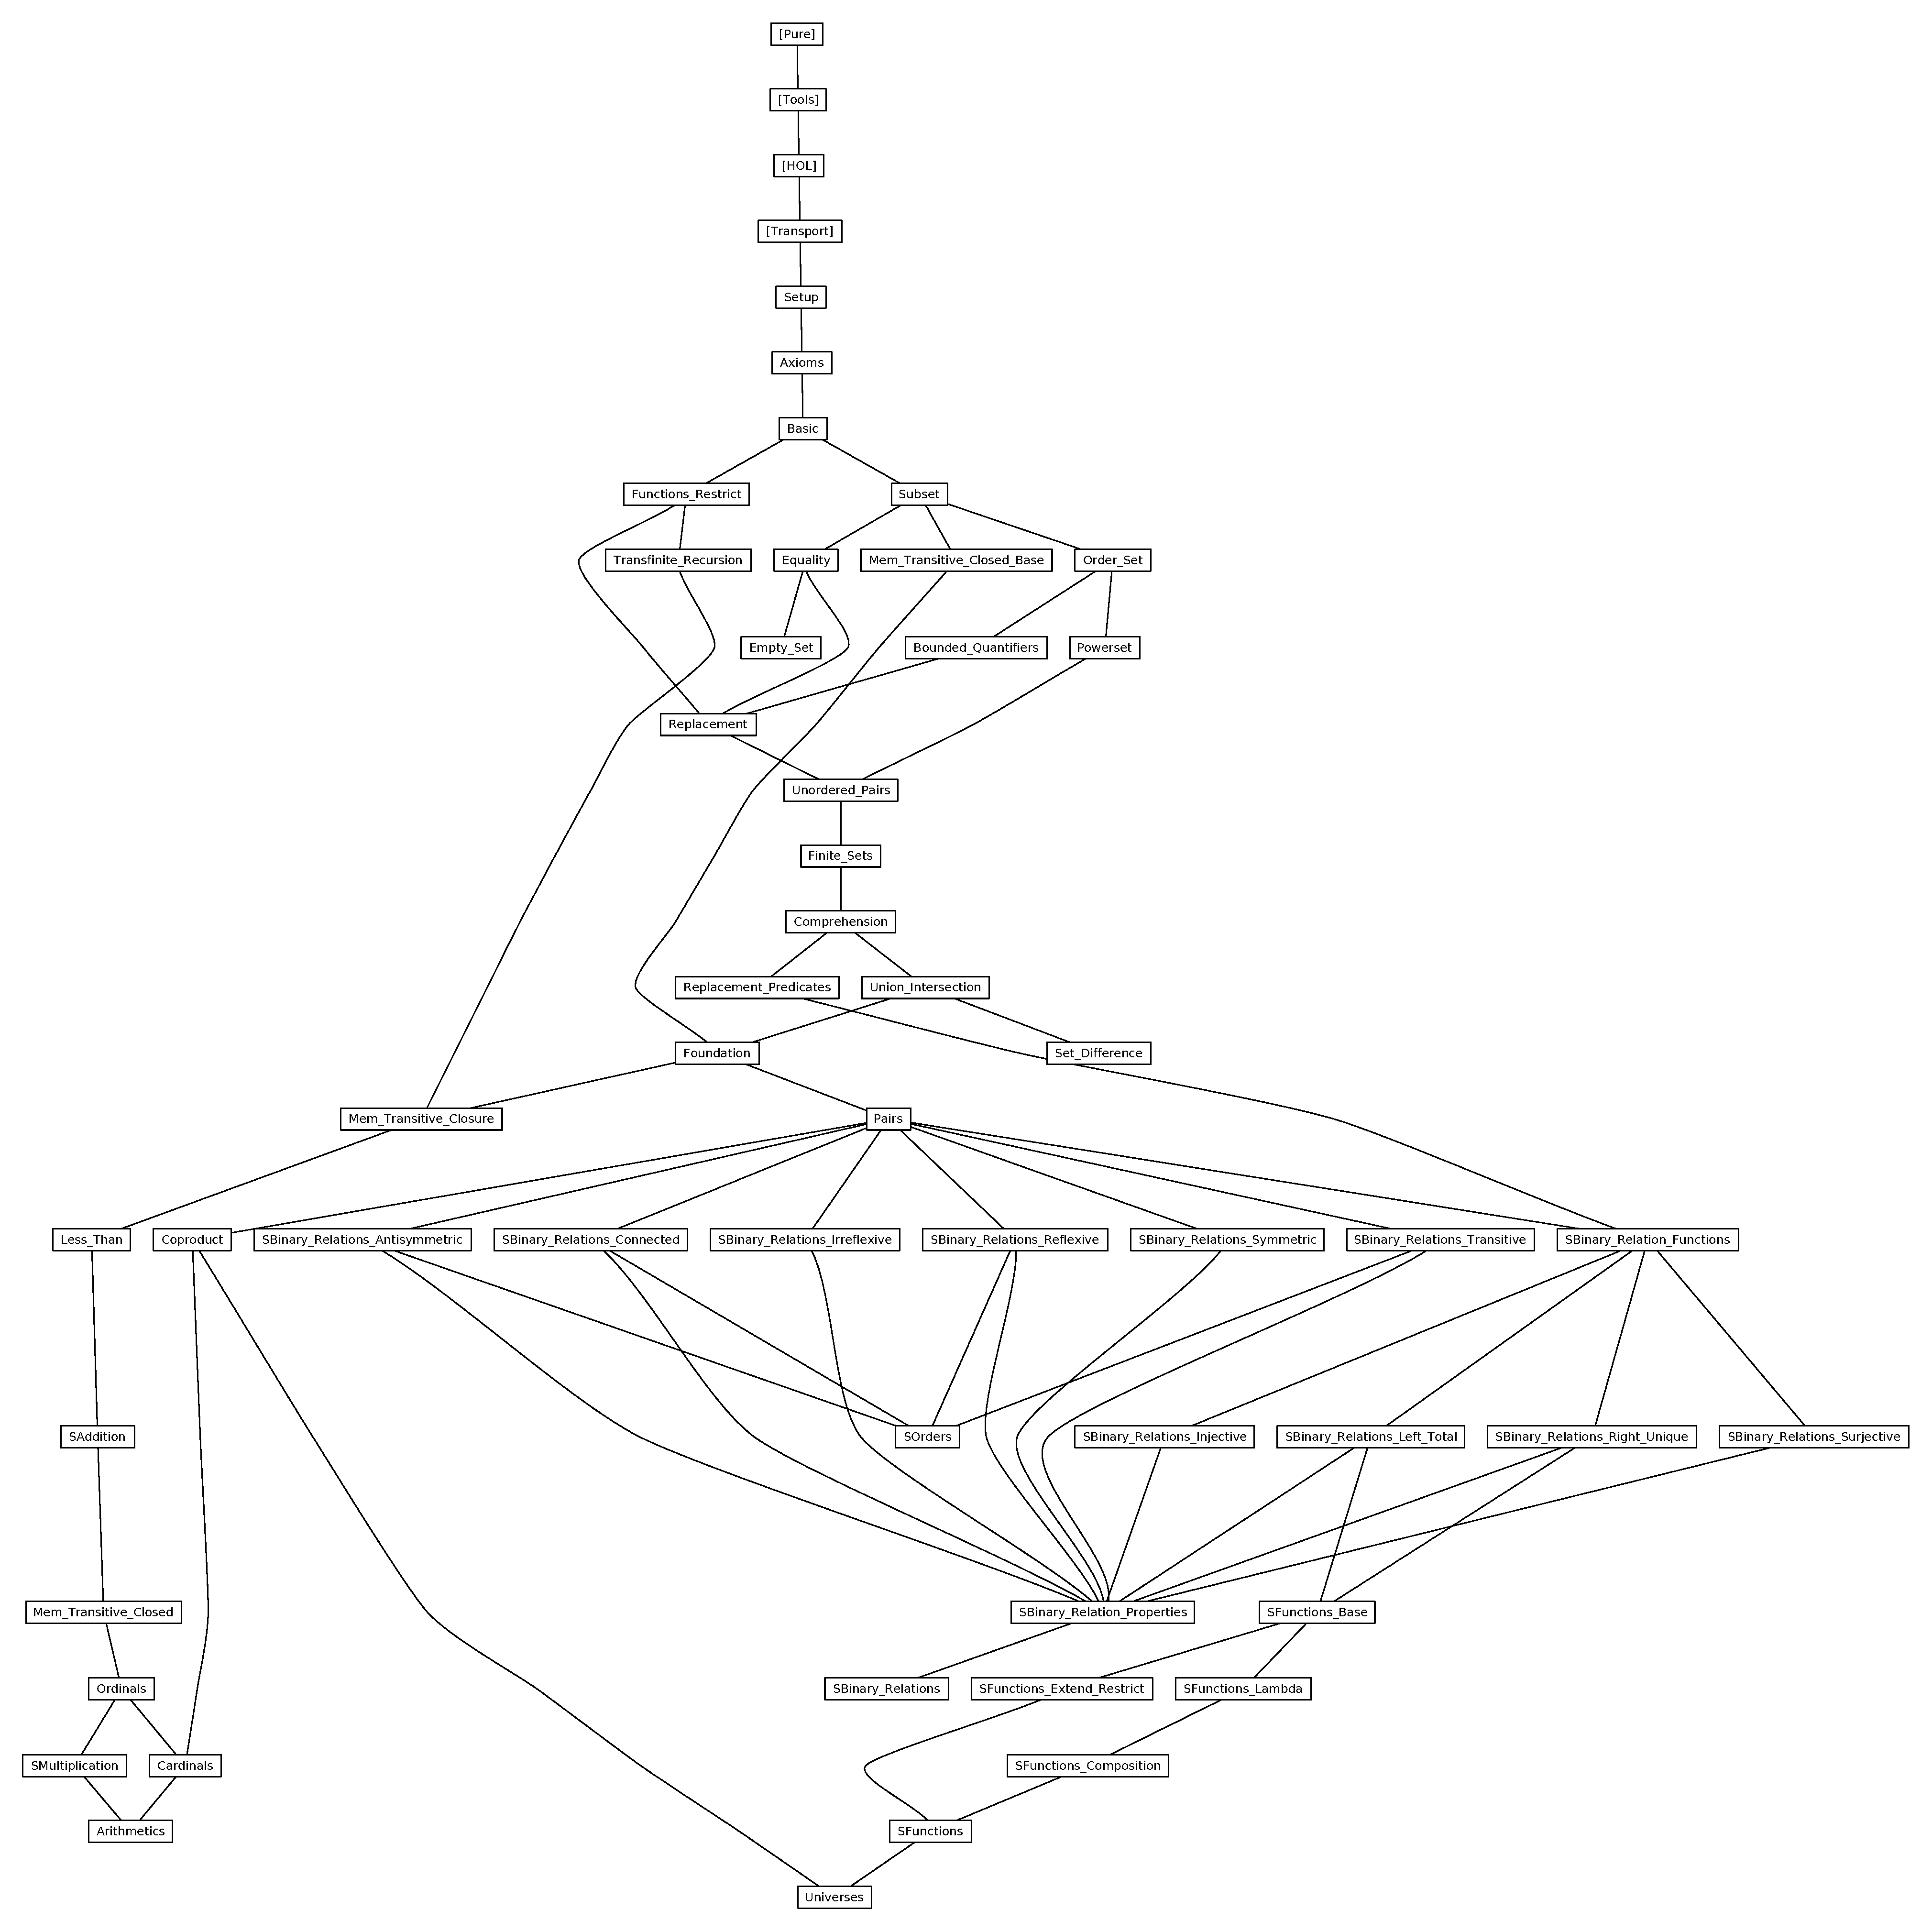
\includegraphics[scale=0.7]{session_graph}
\end{center}

\newpage

\parindent 0pt\parskip 0.5ex

%
\begin{isabellebody}%
\setisabellecontext{Setup}%
%
\isadelimdocument
%
\endisadelimdocument
%
\isatagdocument
%
\isamarkupsection{Setup for Higher-Order Tarski-Grothendieck Set Theory.%
}
\isamarkuptrue%
%
\endisatagdocument
{\isafolddocument}%
%
\isadelimdocument
%
\endisadelimdocument
%
\isadelimtheory
%
\endisadelimtheory
%
\isatagtheory
\isacommand{theory}\isamarkupfalse%
\ Setup\isanewline
\ \ \isakeyword{imports}\ Transport{\isachardot}{\kern0pt}HOL{\isacharunderscore}{\kern0pt}Syntax{\isacharunderscore}{\kern0pt}Bundles{\isacharunderscore}{\kern0pt}Base\isanewline
\isakeyword{begin}%
\endisatagtheory
{\isafoldtheory}%
%
\isadelimtheory
%
\endisadelimtheory
%
\begin{isamarkuptext}%
Remove conflicting HOL-specific syntax.%
\end{isamarkuptext}\isamarkuptrue%
\isacommand{unbundle}\isamarkupfalse%
\ no{\isacharunderscore}{\kern0pt}HOL{\isacharunderscore}{\kern0pt}ascii{\isacharunderscore}{\kern0pt}syntax%
\begin{isamarkuptext}%
Additional logical rules%
\end{isamarkuptext}\isamarkuptrue%
\isacommand{lemma}\isamarkupfalse%
\ or{\isacharunderscore}{\kern0pt}if{\isacharunderscore}{\kern0pt}not{\isacharunderscore}{\kern0pt}imp{\isacharcolon}{\kern0pt}\ {\isachardoublequoteopen}{\isacharparenleft}{\kern0pt}{\isasymnot}A\ {\isasymLongrightarrow}\ B{\isacharparenright}{\kern0pt}\ {\isasymLongrightarrow}\ A\ {\isasymor}\ B{\isachardoublequoteclose}%
\isadelimproof
\ %
\endisadelimproof
%
\isatagproof
\isacommand{by}\isamarkupfalse%
\ blast%
\endisatagproof
{\isafoldproof}%
%
\isadelimproof
%
\endisadelimproof
\isanewline
\isanewline
%
\isadelimtheory
\isanewline
%
\endisadelimtheory
%
\isatagtheory
\isacommand{end}\isamarkupfalse%
%
\endisatagtheory
{\isafoldtheory}%
%
\isadelimtheory
%
\endisadelimtheory
%
\end{isabellebody}%
\endinput
%:%file=~/Documents/github/Isabelle-Set/HOTG/Setup.thy%:%
%:%11=2%:%
%:%27=3%:%
%:%28=3%:%
%:%29=4%:%
%:%30=5%:%
%:%39=7%:%
%:%41=9%:%
%:%42=9%:%
%:%44=11%:%
%:%46=13%:%
%:%47=13%:%
%:%49=13%:%
%:%53=13%:%
%:%54=13%:%
%:%61=13%:%
%:%62=14%:%
%:%65=15%:%
%:%70=16%:%

%
\begin{isabellebody}%
\setisabellecontext{Axioms}%
%
\isadelimdocument
%
\endisadelimdocument
%
\isatagdocument
\isanewline
%
\isamarkupsection{Axioms of Tarski-Grothendieck Set Theory embedded in HOL.%
}
\isamarkuptrue%
%
\endisatagdocument
{\isafolddocument}%
%
\isadelimdocument
%
\endisadelimdocument
%
\isadelimtheory
%
\endisadelimtheory
%
\isatagtheory
\isacommand{theory}\isamarkupfalse%
\ Axioms\isanewline
\ \ \isakeyword{imports}\ Setup\isanewline
\isakeyword{begin}%
\endisatagtheory
{\isafoldtheory}%
%
\isadelimtheory
%
\endisadelimtheory
%
\isadelimdocument
%
\endisadelimdocument
%
\isatagdocument
%
\isamarkupparagraph{Summary%
}
\isamarkuptrue%
%
\endisatagdocument
{\isafolddocument}%
%
\isadelimdocument
%
\endisadelimdocument
%
\begin{isamarkuptext}%
We follow the axiomatisation as described in \cite{brown_et_al:LIPIcs:2019:11064},
who also describe the existence of a model if a 2-inaccessible cardinal exists.%
\end{isamarkuptext}\isamarkuptrue%
%
\begin{isamarkuptext}%
The primitive set type.%
\end{isamarkuptext}\isamarkuptrue%
\isacommand{typedecl}\isamarkupfalse%
\ set%
\begin{isamarkuptext}%
The first four axioms.%
\end{isamarkuptext}\isamarkuptrue%
\isacommand{axiomatization}\isamarkupfalse%
\isanewline
\ \ mem\ \ \ \ \ \ {\isacharcolon}{\kern0pt}{\isacharcolon}{\kern0pt}\ {\isacartoucheopen}set\ {\isasymRightarrow}\ set\ {\isasymRightarrow}\ bool{\isacartoucheclose}\ \isakeyword{and}\isanewline
\ \ emptyset\ {\isacharcolon}{\kern0pt}{\isacharcolon}{\kern0pt}\ {\isacartoucheopen}set{\isacartoucheclose}\ \isakeyword{and}\isanewline
\ \ union\ \ \ \ \ \ \ {\isacharcolon}{\kern0pt}{\isacharcolon}{\kern0pt}\ {\isacartoucheopen}set\ {\isasymRightarrow}\ set{\isacartoucheclose}\ \isakeyword{and}\isanewline
\ \ repl\ \ \ \ \ {\isacharcolon}{\kern0pt}{\isacharcolon}{\kern0pt}\ {\isacartoucheopen}set\ {\isasymRightarrow}\ {\isacharparenleft}{\kern0pt}set\ {\isasymRightarrow}\ set{\isacharparenright}{\kern0pt}\ {\isasymRightarrow}\ set{\isacartoucheclose}\isanewline
\isakeyword{where}\isanewline
\ \ mem{\isacharunderscore}{\kern0pt}induction{\isacharcolon}{\kern0pt}\ {\isachardoublequoteopen}{\isacharparenleft}{\kern0pt}{\isasymforall}X{\isachardot}{\kern0pt}\ {\isacharparenleft}{\kern0pt}{\isasymforall}x{\isachardot}{\kern0pt}\ mem\ x\ X\ {\isasymlongrightarrow}\ P\ x{\isacharparenright}{\kern0pt}\ {\isasymlongrightarrow}\ P\ X{\isacharparenright}{\kern0pt}\ {\isasymlongrightarrow}\ {\isacharparenleft}{\kern0pt}{\isasymforall}X{\isachardot}{\kern0pt}\ P\ X{\isacharparenright}{\kern0pt}{\isachardoublequoteclose}\ \isakeyword{and}\isanewline
\ \ emptyset{\isacharcolon}{\kern0pt}\ {\isachardoublequoteopen}{\isasymnot}{\isacharparenleft}{\kern0pt}{\isasymexists}x{\isachardot}{\kern0pt}\ mem\ x\ emptyset{\isacharparenright}{\kern0pt}{\isachardoublequoteclose}\ \isakeyword{and}\isanewline
\ \ union{\isacharcolon}{\kern0pt}\ {\isachardoublequoteopen}{\isasymforall}X\ x{\isachardot}{\kern0pt}\ mem\ x\ {\isacharparenleft}{\kern0pt}union\ X{\isacharparenright}{\kern0pt}\ {\isasymlongleftrightarrow}\ {\isacharparenleft}{\kern0pt}{\isasymexists}Y{\isachardot}{\kern0pt}\ mem\ Y\ X\ {\isasymand}\ mem\ x\ Y{\isacharparenright}{\kern0pt}{\isachardoublequoteclose}\ \isakeyword{and}\isanewline
\ \ replacement{\isacharcolon}{\kern0pt}\ {\isachardoublequoteopen}{\isasymforall}X\ y{\isachardot}{\kern0pt}\ mem\ y\ {\isacharparenleft}{\kern0pt}repl\ X\ f{\isacharparenright}{\kern0pt}\ {\isasymlongleftrightarrow}\ {\isacharparenleft}{\kern0pt}{\isasymexists}x{\isachardot}{\kern0pt}\ mem\ x\ X\ {\isasymand}\ y\ {\isacharequal}{\kern0pt}\ f\ x{\isacharparenright}{\kern0pt}{\isachardoublequoteclose}%
\begin{isamarkuptext}%
Note: axioms \isa{{\isacharparenleft}{\kern0pt}{\isasymforall}X{\isachardot}{\kern0pt}\ {\isacharparenleft}{\kern0pt}{\isasymforall}x{\isachardot}{\kern0pt}\ mem\ x\ X\ {\isasymlongrightarrow}\ {\isacharquery}{\kern0pt}P\ x{\isacharparenright}{\kern0pt}\ {\isasymlongrightarrow}\ {\isacharquery}{\kern0pt}P\ X{\isacharparenright}{\kern0pt}\ {\isasymlongrightarrow}\ {\isacharparenleft}{\kern0pt}{\isasymforall}X{\isachardot}{\kern0pt}\ {\isacharquery}{\kern0pt}P\ X{\isacharparenright}{\kern0pt}} and \isa{{\isasymforall}X\ y{\isachardot}{\kern0pt}\ mem\ y\ {\isacharparenleft}{\kern0pt}repl\ X\ {\isacharquery}{\kern0pt}f{\isacharparenright}{\kern0pt}\ {\isacharequal}{\kern0pt}\ {\isacharparenleft}{\kern0pt}{\isasymexists}x{\isachardot}{\kern0pt}\ mem\ x\ X\ {\isasymand}\ y\ {\isacharequal}{\kern0pt}\ {\isacharquery}{\kern0pt}f\ x{\isacharparenright}{\kern0pt}} are axiom schemas
in first-order logic. Moreover, \isa{{\isasymforall}X\ y{\isachardot}{\kern0pt}\ mem\ y\ {\isacharparenleft}{\kern0pt}repl\ X\ {\isacharquery}{\kern0pt}f{\isacharparenright}{\kern0pt}\ {\isacharequal}{\kern0pt}\ {\isacharparenleft}{\kern0pt}{\isasymexists}x{\isachardot}{\kern0pt}\ mem\ x\ X\ {\isasymand}\ y\ {\isacharequal}{\kern0pt}\ {\isacharquery}{\kern0pt}f\ x{\isacharparenright}{\kern0pt}} takes a meta-level function \isa{F}.%
\end{isamarkuptext}\isamarkuptrue%
%
\begin{isamarkuptext}%
Let us define some expected notation.%
\end{isamarkuptext}\isamarkuptrue%
\isacommand{bundle}\isamarkupfalse%
\ hotg{\isacharunderscore}{\kern0pt}mem{\isacharunderscore}{\kern0pt}syntax\ \isakeyword{begin}\ \isacommand{notation}\isamarkupfalse%
\ mem\ {\isacharparenleft}{\kern0pt}\isakeyword{infixl}\ {\isachardoublequoteopen}{\isasymin}{\isachardoublequoteclose}\ {\isadigit{5}}{\isadigit{0}}{\isacharparenright}{\kern0pt}\ \isacommand{end}\isamarkupfalse%
\isanewline
\isacommand{bundle}\isamarkupfalse%
\ no{\isacharunderscore}{\kern0pt}hotg{\isacharunderscore}{\kern0pt}mem{\isacharunderscore}{\kern0pt}syntax\ \isakeyword{begin}\ \isacommand{no{\isacharunderscore}{\kern0pt}notation}\isamarkupfalse%
\ mem\ {\isacharparenleft}{\kern0pt}\isakeyword{infixl}\ {\isachardoublequoteopen}{\isasymin}{\isachardoublequoteclose}\ {\isadigit{5}}{\isadigit{0}}{\isacharparenright}{\kern0pt}\ \isacommand{end}\isamarkupfalse%
\isanewline
\isanewline
\isacommand{bundle}\isamarkupfalse%
\ hotg{\isacharunderscore}{\kern0pt}emptyset{\isacharunderscore}{\kern0pt}zero{\isacharunderscore}{\kern0pt}syntax\ \isakeyword{begin}\ \isacommand{notation}\isamarkupfalse%
\ emptyset\ {\isacharparenleft}{\kern0pt}{\isachardoublequoteopen}{\isasymemptyset}{\isachardoublequoteclose}{\isacharparenright}{\kern0pt}\ \isacommand{end}\isamarkupfalse%
\isanewline
\isacommand{bundle}\isamarkupfalse%
\ no{\isacharunderscore}{\kern0pt}hotg{\isacharunderscore}{\kern0pt}emptyset{\isacharunderscore}{\kern0pt}zero{\isacharunderscore}{\kern0pt}syntax\ \isakeyword{begin}\ \isacommand{no{\isacharunderscore}{\kern0pt}notation}\isamarkupfalse%
\ emptyset\ {\isacharparenleft}{\kern0pt}{\isachardoublequoteopen}{\isasymemptyset}{\isachardoublequoteclose}{\isacharparenright}{\kern0pt}\ \isacommand{end}\isamarkupfalse%
\isanewline
\isanewline
\isacommand{bundle}\isamarkupfalse%
\ hotg{\isacharunderscore}{\kern0pt}emptyset{\isacharunderscore}{\kern0pt}braces{\isacharunderscore}{\kern0pt}syntax\ \isakeyword{begin}\ \isacommand{notation}\isamarkupfalse%
\ emptyset\ {\isacharparenleft}{\kern0pt}{\isachardoublequoteopen}{\isacharbraceleft}{\kern0pt}{\isacharbraceright}{\kern0pt}{\isachardoublequoteclose}{\isacharparenright}{\kern0pt}\ \isacommand{end}\isamarkupfalse%
\isanewline
\isacommand{bundle}\isamarkupfalse%
\ no{\isacharunderscore}{\kern0pt}hotg{\isacharunderscore}{\kern0pt}emptyset{\isacharunderscore}{\kern0pt}braces{\isacharunderscore}{\kern0pt}syntax\ \isakeyword{begin}\ \isacommand{no{\isacharunderscore}{\kern0pt}notation}\isamarkupfalse%
\ emptyset\ {\isacharparenleft}{\kern0pt}{\isachardoublequoteopen}{\isacharbraceleft}{\kern0pt}{\isacharbraceright}{\kern0pt}{\isachardoublequoteclose}{\isacharparenright}{\kern0pt}\ \isacommand{end}\isamarkupfalse%
\isanewline
\isanewline
\isacommand{bundle}\isamarkupfalse%
\ hotg{\isacharunderscore}{\kern0pt}emptyset{\isacharunderscore}{\kern0pt}syntax\isanewline
\isakeyword{begin}\isanewline
\ \ \isacommand{unbundle}\isamarkupfalse%
\ hotg{\isacharunderscore}{\kern0pt}emptyset{\isacharunderscore}{\kern0pt}zero{\isacharunderscore}{\kern0pt}syntax\ hotg{\isacharunderscore}{\kern0pt}emptyset{\isacharunderscore}{\kern0pt}braces{\isacharunderscore}{\kern0pt}syntax\isanewline
\isacommand{end}\isamarkupfalse%
\isanewline
\isacommand{bundle}\isamarkupfalse%
\ no{\isacharunderscore}{\kern0pt}hotg{\isacharunderscore}{\kern0pt}emptyset{\isacharunderscore}{\kern0pt}syntax\isanewline
\isakeyword{begin}\isanewline
\ \ \isacommand{unbundle}\isamarkupfalse%
\ no{\isacharunderscore}{\kern0pt}hotg{\isacharunderscore}{\kern0pt}emptyset{\isacharunderscore}{\kern0pt}zero{\isacharunderscore}{\kern0pt}syntax\ no{\isacharunderscore}{\kern0pt}hotg{\isacharunderscore}{\kern0pt}emptyset{\isacharunderscore}{\kern0pt}braces{\isacharunderscore}{\kern0pt}syntax\isanewline
\isacommand{end}\isamarkupfalse%
\isanewline
\isanewline
\isacommand{bundle}\isamarkupfalse%
\ hotg{\isacharunderscore}{\kern0pt}union{\isacharunderscore}{\kern0pt}syntax\ \isakeyword{begin}\ \isacommand{notation}\isamarkupfalse%
\ union\ {\isacharparenleft}{\kern0pt}{\isachardoublequoteopen}{\isasymUnion}{\isacharunderscore}{\kern0pt}{\isachardoublequoteclose}\ {\isacharbrackleft}{\kern0pt}{\isadigit{9}}{\isadigit{0}}{\isacharbrackright}{\kern0pt}\ {\isadigit{9}}{\isadigit{0}}{\isacharparenright}{\kern0pt}\ \isacommand{end}\isamarkupfalse%
\isanewline
\isacommand{bundle}\isamarkupfalse%
\ no{\isacharunderscore}{\kern0pt}hotg{\isacharunderscore}{\kern0pt}union{\isacharunderscore}{\kern0pt}syntax\ \isakeyword{begin}\ \isacommand{no{\isacharunderscore}{\kern0pt}notation}\isamarkupfalse%
\ union\ {\isacharparenleft}{\kern0pt}{\isachardoublequoteopen}{\isasymUnion}{\isacharunderscore}{\kern0pt}{\isachardoublequoteclose}\ {\isacharbrackleft}{\kern0pt}{\isadigit{9}}{\isadigit{0}}{\isacharbrackright}{\kern0pt}\ {\isadigit{9}}{\isadigit{0}}{\isacharparenright}{\kern0pt}\ \isacommand{end}\isamarkupfalse%
\isanewline
\isanewline
\isacommand{unbundle}\isamarkupfalse%
\ hotg{\isacharunderscore}{\kern0pt}mem{\isacharunderscore}{\kern0pt}syntax\ hotg{\isacharunderscore}{\kern0pt}emptyset{\isacharunderscore}{\kern0pt}syntax\ hotg{\isacharunderscore}{\kern0pt}union{\isacharunderscore}{\kern0pt}syntax\isanewline
\isanewline
\isacommand{abbreviation}\isamarkupfalse%
\ {\isacharparenleft}{\kern0pt}input{\isacharparenright}{\kern0pt}\ {\isachardoublequoteopen}mem{\isacharunderscore}{\kern0pt}of\ A\ x\ {\isasymequiv}\ x\ {\isasymin}\ A{\isachardoublequoteclose}\isanewline
\isacommand{abbreviation}\isamarkupfalse%
\ {\isachardoublequoteopen}not{\isacharunderscore}{\kern0pt}mem\ x\ y\ {\isasymequiv}\ {\isasymnot}{\isacharparenleft}{\kern0pt}x\ {\isasymin}\ y{\isacharparenright}{\kern0pt}{\isachardoublequoteclose}\isanewline
\isanewline
\isacommand{bundle}\isamarkupfalse%
\ hotg{\isacharunderscore}{\kern0pt}not{\isacharunderscore}{\kern0pt}mem{\isacharunderscore}{\kern0pt}syntax\ \isakeyword{begin}\ \isacommand{notation}\isamarkupfalse%
\ not{\isacharunderscore}{\kern0pt}mem\ {\isacharparenleft}{\kern0pt}\isakeyword{infixl}\ {\isachardoublequoteopen}{\isasymnotin}{\isachardoublequoteclose}\ {\isadigit{5}}{\isadigit{0}}{\isacharparenright}{\kern0pt}\ \isacommand{end}\isamarkupfalse%
\isanewline
\isacommand{bundle}\isamarkupfalse%
\ no{\isacharunderscore}{\kern0pt}hotg{\isacharunderscore}{\kern0pt}not{\isacharunderscore}{\kern0pt}mem{\isacharunderscore}{\kern0pt}syntax\ \isakeyword{begin}\ \isacommand{no{\isacharunderscore}{\kern0pt}notation}\isamarkupfalse%
\ not{\isacharunderscore}{\kern0pt}mem\ {\isacharparenleft}{\kern0pt}\isakeyword{infixl}\ {\isachardoublequoteopen}{\isasymnotin}{\isachardoublequoteclose}\ {\isadigit{5}}{\isadigit{0}}{\isacharparenright}{\kern0pt}\ \isacommand{end}\isamarkupfalse%
\isanewline
\isanewline
\isacommand{unbundle}\isamarkupfalse%
\ hotg{\isacharunderscore}{\kern0pt}not{\isacharunderscore}{\kern0pt}mem{\isacharunderscore}{\kern0pt}syntax%
\begin{isamarkuptext}%
Based on the membership relation, we can define the subset relation.%
\end{isamarkuptext}\isamarkuptrue%
\isacommand{definition}\isamarkupfalse%
\ subset\ {\isacharcolon}{\kern0pt}{\isacharcolon}{\kern0pt}\ {\isacartoucheopen}set\ {\isasymRightarrow}\ set\ {\isasymRightarrow}\ bool{\isacartoucheclose}\isanewline
\ \ \isakeyword{where}\ {\isachardoublequoteopen}subset\ A\ B\ {\isasymequiv}\ {\isasymforall}x{\isachardot}{\kern0pt}\ x\ {\isasymin}\ A\ {\isasymlongrightarrow}\ x\ {\isasymin}\ B{\isachardoublequoteclose}%
\begin{isamarkuptext}%
Again, we define some notation.%
\end{isamarkuptext}\isamarkuptrue%
\isacommand{bundle}\isamarkupfalse%
\ hotg{\isacharunderscore}{\kern0pt}subset{\isacharunderscore}{\kern0pt}syntax\ \isakeyword{begin}\ \isacommand{notation}\isamarkupfalse%
\ subset\ {\isacharparenleft}{\kern0pt}\isakeyword{infixl}\ {\isachardoublequoteopen}{\isasymsubseteq}{\isachardoublequoteclose}\ {\isadigit{5}}{\isadigit{0}}{\isacharparenright}{\kern0pt}\ \isacommand{end}\isamarkupfalse%
\isanewline
\isacommand{bundle}\isamarkupfalse%
\ no{\isacharunderscore}{\kern0pt}hotg{\isacharunderscore}{\kern0pt}subset{\isacharunderscore}{\kern0pt}syntax\ \isakeyword{begin}\ \isacommand{no{\isacharunderscore}{\kern0pt}notation}\isamarkupfalse%
\ subset\ {\isacharparenleft}{\kern0pt}\isakeyword{infixl}\ {\isachardoublequoteopen}{\isasymsubseteq}{\isachardoublequoteclose}\ {\isadigit{5}}{\isadigit{0}}{\isacharparenright}{\kern0pt}\ \isacommand{end}\isamarkupfalse%
\isanewline
\isanewline
\isacommand{unbundle}\isamarkupfalse%
\ hotg{\isacharunderscore}{\kern0pt}subset{\isacharunderscore}{\kern0pt}syntax%
\begin{isamarkuptext}%
The axiom of extensionality and powerset.%
\end{isamarkuptext}\isamarkuptrue%
\isacommand{axiomatization}\isamarkupfalse%
\isanewline
\ \ powerset\ {\isacharcolon}{\kern0pt}{\isacharcolon}{\kern0pt}\ {\isacartoucheopen}set\ {\isasymRightarrow}\ set{\isacartoucheclose}\isanewline
\isakeyword{where}\isanewline
\ \ extensionality{\isacharcolon}{\kern0pt}\ {\isachardoublequoteopen}{\isasymforall}X\ Y{\isachardot}{\kern0pt}\ X\ {\isasymsubseteq}\ Y\ {\isasymlongrightarrow}\ Y\ {\isasymsubseteq}\ X\ {\isasymlongrightarrow}\ X\ {\isacharequal}{\kern0pt}\ Y{\isachardoublequoteclose}\ \isakeyword{and}\isanewline
\ \ powerset{\isacharcolon}{\kern0pt}\ {\isachardoublequoteopen}{\isasymforall}A\ x{\isachardot}{\kern0pt}\ x\ {\isasymin}\ powerset\ A\ {\isasymlongleftrightarrow}\ x\ {\isasymsubseteq}\ A{\isachardoublequoteclose}%
\begin{isamarkuptext}%
Lastly, we want to axiomatise the existence of Grothendieck universes.
This can be done in different ways. We again follow the approach from
\cite{brown_et_al:LIPIcs:2019:11064}.%
\end{isamarkuptext}\isamarkuptrue%
\isacommand{definition}\isamarkupfalse%
\ mem{\isacharunderscore}{\kern0pt}trans{\isacharunderscore}{\kern0pt}closed\ {\isacharcolon}{\kern0pt}{\isacharcolon}{\kern0pt}\ {\isacartoucheopen}set\ {\isasymRightarrow}\ bool{\isacartoucheclose}\isanewline
\ \ \isakeyword{where}\ {\isachardoublequoteopen}mem{\isacharunderscore}{\kern0pt}trans{\isacharunderscore}{\kern0pt}closed\ X\ {\isasymequiv}\ {\isacharparenleft}{\kern0pt}{\isasymforall}x{\isachardot}{\kern0pt}\ x\ {\isasymin}\ X\ {\isasymlongrightarrow}\ x\ {\isasymsubseteq}\ X{\isacharparenright}{\kern0pt}{\isachardoublequoteclose}\isanewline
\isanewline
\isacommand{definition}\isamarkupfalse%
\ ZF{\isacharunderscore}{\kern0pt}closed\ {\isacharcolon}{\kern0pt}{\isacharcolon}{\kern0pt}\ {\isacartoucheopen}set\ {\isasymRightarrow}\ bool{\isacartoucheclose}\isanewline
\ \ \isakeyword{where}\ {\isachardoublequoteopen}ZF{\isacharunderscore}{\kern0pt}closed\ U\ {\isasymequiv}\ {\isacharparenleft}{\kern0pt}\isanewline
\ \ \ \ {\isacharparenleft}{\kern0pt}{\isasymforall}X{\isachardot}{\kern0pt}\ X\ {\isasymin}\ U\ {\isasymlongrightarrow}\ {\isasymUnion}X\ {\isasymin}\ U{\isacharparenright}{\kern0pt}\ {\isasymand}\isanewline
\ \ \ \ {\isacharparenleft}{\kern0pt}{\isasymforall}X{\isachardot}{\kern0pt}\ X\ {\isasymin}\ U\ {\isasymlongrightarrow}\ powerset\ X\ {\isasymin}\ U{\isacharparenright}{\kern0pt}\ {\isasymand}\isanewline
\ \ \ \ {\isacharparenleft}{\kern0pt}{\isasymforall}X\ F{\isachardot}{\kern0pt}\ X\ {\isasymin}\ U\ {\isasymlongrightarrow}\ {\isacharparenleft}{\kern0pt}{\isasymforall}x{\isachardot}{\kern0pt}\ x\ {\isasymin}\ X\ {\isasymlongrightarrow}\ F\ x\ {\isasymin}\ U{\isacharparenright}{\kern0pt}\ {\isasymlongrightarrow}\ repl\ X\ F\ {\isasymin}\ U{\isacharparenright}{\kern0pt}\isanewline
\ \ {\isacharparenright}{\kern0pt}{\isachardoublequoteclose}%
\begin{isamarkuptext}%
Note that \isa{ZF{\isacharunderscore}{\kern0pt}closed} is a second-order statement.%
\end{isamarkuptext}\isamarkuptrue%
%
\begin{isamarkuptext}%
\isa{univ\ X} is the smallest Grothendieck universe containing X.%
\end{isamarkuptext}\isamarkuptrue%
\isacommand{axiomatization}\isamarkupfalse%
\isanewline
\ \ univ\ {\isacharcolon}{\kern0pt}{\isacharcolon}{\kern0pt}\ {\isacartoucheopen}set\ {\isasymRightarrow}\ set{\isacartoucheclose}\isanewline
\isakeyword{where}\isanewline
\ \ mem{\isacharunderscore}{\kern0pt}univ\ {\isacharbrackleft}{\kern0pt}iff{\isacharbrackright}{\kern0pt}{\isacharcolon}{\kern0pt}\ {\isachardoublequoteopen}X\ {\isasymin}\ univ\ X{\isachardoublequoteclose}\ \isakeyword{and}\isanewline
\ \ mem{\isacharunderscore}{\kern0pt}trans{\isacharunderscore}{\kern0pt}closed{\isacharunderscore}{\kern0pt}univ\ {\isacharbrackleft}{\kern0pt}iff{\isacharbrackright}{\kern0pt}{\isacharcolon}{\kern0pt}\ {\isachardoublequoteopen}mem{\isacharunderscore}{\kern0pt}trans{\isacharunderscore}{\kern0pt}closed\ {\isacharparenleft}{\kern0pt}univ\ X{\isacharparenright}{\kern0pt}{\isachardoublequoteclose}\ \isakeyword{and}\isanewline
\ \ ZF{\isacharunderscore}{\kern0pt}closed{\isacharunderscore}{\kern0pt}univ\ {\isacharbrackleft}{\kern0pt}iff{\isacharbrackright}{\kern0pt}{\isacharcolon}{\kern0pt}\ {\isachardoublequoteopen}ZF{\isacharunderscore}{\kern0pt}closed\ {\isacharparenleft}{\kern0pt}univ\ X{\isacharparenright}{\kern0pt}{\isachardoublequoteclose}\ \isakeyword{and}\isanewline
\ \ univ{\isacharunderscore}{\kern0pt}min{\isacharcolon}{\kern0pt}\ {\isachardoublequoteopen}{\isasymlbrakk}X\ {\isasymin}\ U{\isacharsemicolon}{\kern0pt}\ mem{\isacharunderscore}{\kern0pt}trans{\isacharunderscore}{\kern0pt}closed\ U{\isacharsemicolon}{\kern0pt}\ ZF{\isacharunderscore}{\kern0pt}closed\ U{\isasymrbrakk}\ {\isasymLongrightarrow}\ univ\ X\ {\isasymsubseteq}\ U{\isachardoublequoteclose}\isanewline
\isanewline
\isanewline
\isacommand{bundle}\isamarkupfalse%
\ hotg{\isacharunderscore}{\kern0pt}basic{\isacharunderscore}{\kern0pt}syntax\isanewline
\isakeyword{begin}\isanewline
\ \ \isacommand{unbundle}\isamarkupfalse%
\isanewline
\ \ \ \ hotg{\isacharunderscore}{\kern0pt}mem{\isacharunderscore}{\kern0pt}syntax\isanewline
\ \ \ \ hotg{\isacharunderscore}{\kern0pt}not{\isacharunderscore}{\kern0pt}mem{\isacharunderscore}{\kern0pt}syntax\isanewline
\ \ \ \ hotg{\isacharunderscore}{\kern0pt}emptyset{\isacharunderscore}{\kern0pt}syntax\isanewline
\ \ \ \ hotg{\isacharunderscore}{\kern0pt}union{\isacharunderscore}{\kern0pt}syntax\isanewline
\ \ \ \ hotg{\isacharunderscore}{\kern0pt}subset{\isacharunderscore}{\kern0pt}syntax\isanewline
\isacommand{end}\isamarkupfalse%
\isanewline
\isacommand{bundle}\isamarkupfalse%
\ no{\isacharunderscore}{\kern0pt}hotg{\isacharunderscore}{\kern0pt}basic{\isacharunderscore}{\kern0pt}syntax\isanewline
\isakeyword{begin}\isanewline
\ \ \isacommand{unbundle}\isamarkupfalse%
\isanewline
\ \ \ \ no{\isacharunderscore}{\kern0pt}hotg{\isacharunderscore}{\kern0pt}mem{\isacharunderscore}{\kern0pt}syntax\isanewline
\ \ \ \ no{\isacharunderscore}{\kern0pt}hotg{\isacharunderscore}{\kern0pt}not{\isacharunderscore}{\kern0pt}mem{\isacharunderscore}{\kern0pt}syntax\isanewline
\ \ \ \ no{\isacharunderscore}{\kern0pt}hotg{\isacharunderscore}{\kern0pt}emptyset{\isacharunderscore}{\kern0pt}syntax\isanewline
\ \ \ \ no{\isacharunderscore}{\kern0pt}hotg{\isacharunderscore}{\kern0pt}union{\isacharunderscore}{\kern0pt}syntax\isanewline
\ \ \ \ no{\isacharunderscore}{\kern0pt}hotg{\isacharunderscore}{\kern0pt}subset{\isacharunderscore}{\kern0pt}syntax\isanewline
\isacommand{end}\isamarkupfalse%
\isanewline
%
\isadelimtheory
\isanewline
%
\endisadelimtheory
%
\isatagtheory
\isacommand{end}\isamarkupfalse%
%
\endisatagtheory
{\isafoldtheory}%
%
\isadelimtheory
%
\endisadelimtheory
%
\end{isabellebody}%
\endinput
%:%file=~/Documents/github/Isabelle-Set/HOTG/Axioms.thy%:%
%:%10=1%:%
%:%12=3%:%
%:%28=4%:%
%:%29=4%:%
%:%30=5%:%
%:%31=6%:%
%:%45=7%:%
%:%57=8%:%
%:%58=9%:%
%:%62=11%:%
%:%64=12%:%
%:%65=12%:%
%:%67=14%:%
%:%69=15%:%
%:%70=15%:%
%:%71=16%:%
%:%72=17%:%
%:%73=18%:%
%:%74=19%:%
%:%75=20%:%
%:%76=21%:%
%:%77=22%:%
%:%78=23%:%
%:%79=24%:%
%:%81=26%:%
%:%82=27%:%
%:%86=29%:%
%:%88=31%:%
%:%89=31%:%
%:%90=31%:%
%:%91=31%:%
%:%92=32%:%
%:%93=32%:%
%:%94=32%:%
%:%95=32%:%
%:%96=33%:%
%:%97=34%:%
%:%98=34%:%
%:%99=34%:%
%:%100=34%:%
%:%101=35%:%
%:%102=35%:%
%:%103=35%:%
%:%104=35%:%
%:%105=36%:%
%:%106=37%:%
%:%107=37%:%
%:%108=37%:%
%:%109=37%:%
%:%110=38%:%
%:%111=38%:%
%:%112=38%:%
%:%113=38%:%
%:%114=39%:%
%:%115=40%:%
%:%116=40%:%
%:%117=41%:%
%:%118=42%:%
%:%119=42%:%
%:%120=43%:%
%:%121=43%:%
%:%122=44%:%
%:%123=44%:%
%:%124=45%:%
%:%125=46%:%
%:%126=46%:%
%:%127=47%:%
%:%128=47%:%
%:%129=48%:%
%:%130=49%:%
%:%131=49%:%
%:%132=49%:%
%:%133=49%:%
%:%134=50%:%
%:%135=50%:%
%:%136=50%:%
%:%137=50%:%
%:%138=51%:%
%:%139=52%:%
%:%140=52%:%
%:%141=53%:%
%:%142=54%:%
%:%143=54%:%
%:%144=55%:%
%:%145=55%:%
%:%146=56%:%
%:%147=57%:%
%:%148=57%:%
%:%149=57%:%
%:%150=57%:%
%:%151=58%:%
%:%152=58%:%
%:%153=58%:%
%:%154=58%:%
%:%155=59%:%
%:%156=60%:%
%:%157=60%:%
%:%159=63%:%
%:%161=64%:%
%:%162=64%:%
%:%163=65%:%
%:%165=67%:%
%:%167=68%:%
%:%168=68%:%
%:%169=68%:%
%:%170=68%:%
%:%171=69%:%
%:%172=69%:%
%:%173=69%:%
%:%174=69%:%
%:%175=70%:%
%:%176=71%:%
%:%177=71%:%
%:%179=73%:%
%:%181=74%:%
%:%182=74%:%
%:%183=75%:%
%:%184=76%:%
%:%185=77%:%
%:%186=78%:%
%:%188=80%:%
%:%189=81%:%
%:%190=82%:%
%:%192=84%:%
%:%193=84%:%
%:%194=85%:%
%:%195=86%:%
%:%196=87%:%
%:%197=87%:%
%:%198=88%:%
%:%204=94%:%
%:%208=96%:%
%:%210=98%:%
%:%211=98%:%
%:%212=99%:%
%:%213=100%:%
%:%214=101%:%
%:%215=102%:%
%:%216=103%:%
%:%217=104%:%
%:%218=105%:%
%:%219=106%:%
%:%220=107%:%
%:%221=107%:%
%:%222=108%:%
%:%223=109%:%
%:%224=109%:%
%:%225=110%:%
%:%226=111%:%
%:%227=112%:%
%:%228=113%:%
%:%229=114%:%
%:%230=115%:%
%:%231=115%:%
%:%232=116%:%
%:%233=116%:%
%:%234=117%:%
%:%235=118%:%
%:%236=118%:%
%:%237=119%:%
%:%238=120%:%
%:%239=121%:%
%:%240=122%:%
%:%241=123%:%
%:%242=124%:%
%:%243=124%:%
%:%246=125%:%
%:%251=126%:%

%
\begin{isabellebody}%
\setisabellecontext{Basic}%
%
\isadelimdocument
%
\endisadelimdocument
%
\isatagdocument
%
\isamarkupsection{Basic Lemmas%
}
\isamarkuptrue%
%
\endisatagdocument
{\isafolddocument}%
%
\isadelimdocument
%
\endisadelimdocument
%
\isadelimtheory
%
\endisadelimtheory
%
\isatagtheory
\isacommand{theory}\isamarkupfalse%
\ Basic\isanewline
\ \ \isakeyword{imports}\ Axioms\isanewline
\isakeyword{begin}%
\endisatagtheory
{\isafoldtheory}%
%
\isadelimtheory
%
\endisadelimtheory
%
\isadelimdocument
%
\endisadelimdocument
%
\isatagdocument
%
\isamarkupparagraph{Summary%
}
\isamarkuptrue%
%
\endisatagdocument
{\isafolddocument}%
%
\isadelimdocument
%
\endisadelimdocument
%
\begin{isamarkuptext}%
Here we derive a few preliminary lemmas following from the axioms that are
needed to formalise more complicated concepts.%
\end{isamarkuptext}\isamarkuptrue%
%
\begin{isamarkuptext}%
The following are easier to work with variants of the axioms.%
\end{isamarkuptext}\isamarkuptrue%
\isacommand{lemma}\isamarkupfalse%
\ not{\isacharunderscore}{\kern0pt}mem{\isacharunderscore}{\kern0pt}emptyset\ {\isacharbrackleft}{\kern0pt}iff{\isacharbrackright}{\kern0pt}{\isacharcolon}{\kern0pt}\ {\isachardoublequoteopen}x\ {\isasymnotin}\ {\isacharbraceleft}{\kern0pt}{\isacharbraceright}{\kern0pt}{\isachardoublequoteclose}%
\isadelimproof
\ %
\endisadelimproof
%
\isatagproof
\isacommand{using}\isamarkupfalse%
\ emptyset\ \isacommand{by}\isamarkupfalse%
\ blast%
\endisatagproof
{\isafoldproof}%
%
\isadelimproof
%
\endisadelimproof
\isanewline
\isanewline
\isacommand{lemma}\isamarkupfalse%
\ eq{\isacharunderscore}{\kern0pt}if{\isacharunderscore}{\kern0pt}subset{\isacharunderscore}{\kern0pt}if{\isacharunderscore}{\kern0pt}subset\ {\isacharbrackleft}{\kern0pt}intro{\isacharbrackright}{\kern0pt}{\isacharcolon}{\kern0pt}\ {\isachardoublequoteopen}{\isasymlbrakk}X\ {\isasymsubseteq}\ Y{\isacharsemicolon}{\kern0pt}\ Y\ {\isasymsubseteq}\ X{\isasymrbrakk}\ {\isasymLongrightarrow}\ X\ {\isacharequal}{\kern0pt}\ Y{\isachardoublequoteclose}\isanewline
%
\isadelimproof
\ \ %
\endisadelimproof
%
\isatagproof
\isacommand{by}\isamarkupfalse%
\ {\isacharparenleft}{\kern0pt}fact\ Axioms{\isachardot}{\kern0pt}extensionality{\isacharbrackleft}{\kern0pt}rule{\isacharunderscore}{\kern0pt}format{\isacharbrackright}{\kern0pt}{\isacharparenright}{\kern0pt}%
\endisatagproof
{\isafoldproof}%
%
\isadelimproof
\isanewline
%
\endisadelimproof
\isanewline
\isacommand{lemma}\isamarkupfalse%
\ mem{\isacharunderscore}{\kern0pt}induction\ {\isacharbrackleft}{\kern0pt}case{\isacharunderscore}{\kern0pt}names\ mem{\isacharcomma}{\kern0pt}\ induct\ type{\isacharcolon}{\kern0pt}\ set{\isacharbrackright}{\kern0pt}{\isacharcolon}{\kern0pt}\isanewline
\ \ {\isachardoublequoteopen}{\isacharparenleft}{\kern0pt}{\isasymAnd}X{\isachardot}{\kern0pt}\ {\isacharparenleft}{\kern0pt}{\isasymAnd}x{\isachardot}{\kern0pt}\ x\ {\isasymin}\ X\ {\isasymLongrightarrow}\ P\ x{\isacharparenright}{\kern0pt}\ {\isasymLongrightarrow}\ P\ X{\isacharparenright}{\kern0pt}\ {\isasymLongrightarrow}\ P\ X{\isachardoublequoteclose}\isanewline
%
\isadelimproof
\ \ %
\endisadelimproof
%
\isatagproof
\isacommand{by}\isamarkupfalse%
\ {\isacharparenleft}{\kern0pt}fact\ Axioms{\isachardot}{\kern0pt}mem{\isacharunderscore}{\kern0pt}induction{\isacharbrackleft}{\kern0pt}rule{\isacharunderscore}{\kern0pt}format{\isacharbrackright}{\kern0pt}{\isacharparenright}{\kern0pt}%
\endisatagproof
{\isafoldproof}%
%
\isadelimproof
\isanewline
%
\endisadelimproof
\isanewline
\isacommand{lemma}\isamarkupfalse%
\ mem{\isacharunderscore}{\kern0pt}union{\isacharunderscore}{\kern0pt}iff{\isacharunderscore}{\kern0pt}mem{\isacharunderscore}{\kern0pt}mem\ {\isacharbrackleft}{\kern0pt}iff{\isacharbrackright}{\kern0pt}{\isacharcolon}{\kern0pt}\ {\isachardoublequoteopen}{\isacharparenleft}{\kern0pt}x\ {\isasymin}\ {\isasymUnion}X{\isacharparenright}{\kern0pt}\ {\isasymlongleftrightarrow}\ {\isacharparenleft}{\kern0pt}{\isasymexists}Y{\isachardot}{\kern0pt}\ Y\ {\isasymin}\ X\ {\isasymand}\ x\ {\isasymin}\ Y{\isacharparenright}{\kern0pt}{\isachardoublequoteclose}\isanewline
%
\isadelimproof
\ \ %
\endisadelimproof
%
\isatagproof
\isacommand{by}\isamarkupfalse%
\ {\isacharparenleft}{\kern0pt}fact\ Axioms{\isachardot}{\kern0pt}union{\isacharbrackleft}{\kern0pt}rule{\isacharunderscore}{\kern0pt}format{\isacharbrackright}{\kern0pt}{\isacharparenright}{\kern0pt}%
\endisatagproof
{\isafoldproof}%
%
\isadelimproof
\isanewline
%
\endisadelimproof
\isanewline
\isacommand{corollary}\isamarkupfalse%
\ mem{\isacharunderscore}{\kern0pt}unionI{\isacharcolon}{\kern0pt}\isanewline
\ \ \isakeyword{assumes}\ {\isachardoublequoteopen}Y\ {\isasymin}\ X{\isachardoublequoteclose}\isanewline
\ \ \isakeyword{and}\ {\isachardoublequoteopen}x\ {\isasymin}\ Y{\isachardoublequoteclose}\isanewline
\ \ \isakeyword{shows}\ {\isachardoublequoteopen}x\ {\isasymin}\ {\isasymUnion}X{\isachardoublequoteclose}\isanewline
%
\isadelimproof
\ \ %
\endisadelimproof
%
\isatagproof
\isacommand{using}\isamarkupfalse%
\ assms\ mem{\isacharunderscore}{\kern0pt}union{\isacharunderscore}{\kern0pt}iff{\isacharunderscore}{\kern0pt}mem{\isacharunderscore}{\kern0pt}mem\ \isacommand{by}\isamarkupfalse%
\ auto%
\endisatagproof
{\isafoldproof}%
%
\isadelimproof
\isanewline
%
\endisadelimproof
\isanewline
\isacommand{corollary}\isamarkupfalse%
\ mem{\isacharunderscore}{\kern0pt}unionE{\isacharcolon}{\kern0pt}\isanewline
\ \ \isakeyword{assumes}\ {\isachardoublequoteopen}x\ {\isasymin}\ {\isasymUnion}X{\isachardoublequoteclose}\isanewline
\ \ \isakeyword{obtains}\ Y\ \isakeyword{where}\ {\isachardoublequoteopen}Y\ {\isasymin}\ X{\isachardoublequoteclose}\ {\isachardoublequoteopen}x\ {\isasymin}\ Y{\isachardoublequoteclose}\isanewline
%
\isadelimproof
\ \ %
\endisadelimproof
%
\isatagproof
\isacommand{using}\isamarkupfalse%
\ assms\ mem{\isacharunderscore}{\kern0pt}union{\isacharunderscore}{\kern0pt}iff{\isacharunderscore}{\kern0pt}mem{\isacharunderscore}{\kern0pt}mem\ \isacommand{by}\isamarkupfalse%
\ auto%
\endisatagproof
{\isafoldproof}%
%
\isadelimproof
\isanewline
%
\endisadelimproof
\isanewline
\isacommand{lemma}\isamarkupfalse%
\ mem{\isacharunderscore}{\kern0pt}powerset{\isacharunderscore}{\kern0pt}iff{\isacharunderscore}{\kern0pt}subset\ {\isacharbrackleft}{\kern0pt}iff{\isacharbrackright}{\kern0pt}{\isacharcolon}{\kern0pt}\ {\isachardoublequoteopen}{\isacharparenleft}{\kern0pt}x\ {\isasymin}\ powerset\ A{\isacharparenright}{\kern0pt}\ {\isasymlongleftrightarrow}\ {\isacharparenleft}{\kern0pt}x\ {\isasymsubseteq}\ A{\isacharparenright}{\kern0pt}{\isachardoublequoteclose}\isanewline
%
\isadelimproof
\ \ %
\endisadelimproof
%
\isatagproof
\isacommand{by}\isamarkupfalse%
\ {\isacharparenleft}{\kern0pt}fact\ Axioms{\isachardot}{\kern0pt}powerset{\isacharbrackleft}{\kern0pt}rule{\isacharunderscore}{\kern0pt}format{\isacharbrackright}{\kern0pt}{\isacharparenright}{\kern0pt}%
\endisatagproof
{\isafoldproof}%
%
\isadelimproof
\isanewline
%
\endisadelimproof
\isanewline
\isacommand{corollary}\isamarkupfalse%
\ mem{\isacharunderscore}{\kern0pt}powerset{\isacharunderscore}{\kern0pt}if{\isacharunderscore}{\kern0pt}subset{\isacharcolon}{\kern0pt}\isanewline
\ \ \isakeyword{assumes}\ {\isachardoublequoteopen}x\ {\isasymsubseteq}\ A{\isachardoublequoteclose}\isanewline
\ \ \isakeyword{shows}\ {\isachardoublequoteopen}x\ {\isasymin}\ powerset\ A{\isachardoublequoteclose}\isanewline
%
\isadelimproof
\ \ %
\endisadelimproof
%
\isatagproof
\isacommand{using}\isamarkupfalse%
\ assms\ \isacommand{by}\isamarkupfalse%
\ blast%
\endisatagproof
{\isafoldproof}%
%
\isadelimproof
\isanewline
%
\endisadelimproof
\isanewline
\isacommand{corollary}\isamarkupfalse%
\ subset{\isacharunderscore}{\kern0pt}if{\isacharunderscore}{\kern0pt}mem{\isacharunderscore}{\kern0pt}powerset{\isacharcolon}{\kern0pt}\isanewline
\ \ \isakeyword{assumes}\ {\isachardoublequoteopen}x\ {\isasymin}\ powerset\ A{\isachardoublequoteclose}\isanewline
\ \ \isakeyword{shows}\ {\isachardoublequoteopen}x\ {\isasymsubseteq}\ A{\isachardoublequoteclose}\isanewline
%
\isadelimproof
\ \ %
\endisadelimproof
%
\isatagproof
\isacommand{using}\isamarkupfalse%
\ assms\ \isacommand{by}\isamarkupfalse%
\ blast%
\endisatagproof
{\isafoldproof}%
%
\isadelimproof
\isanewline
%
\endisadelimproof
\isanewline
\isacommand{lemma}\isamarkupfalse%
\ mem{\isacharunderscore}{\kern0pt}repl{\isacharunderscore}{\kern0pt}iff{\isacharunderscore}{\kern0pt}mem{\isacharunderscore}{\kern0pt}eq\ {\isacharbrackleft}{\kern0pt}iff{\isacharbrackright}{\kern0pt}{\isacharcolon}{\kern0pt}\ {\isachardoublequoteopen}{\isacharparenleft}{\kern0pt}y\ {\isasymin}\ repl\ X\ f{\isacharparenright}{\kern0pt}\ {\isasymlongleftrightarrow}\ {\isacharparenleft}{\kern0pt}{\isasymexists}x{\isachardot}{\kern0pt}\ x\ {\isasymin}\ X\ {\isasymand}\ y\ {\isacharequal}{\kern0pt}\ f\ x{\isacharparenright}{\kern0pt}{\isachardoublequoteclose}\isanewline
%
\isadelimproof
\ \ %
\endisadelimproof
%
\isatagproof
\isacommand{by}\isamarkupfalse%
\ {\isacharparenleft}{\kern0pt}fact\ Axioms{\isachardot}{\kern0pt}replacement{\isacharbrackleft}{\kern0pt}rule{\isacharunderscore}{\kern0pt}format{\isacharbrackright}{\kern0pt}{\isacharparenright}{\kern0pt}%
\endisatagproof
{\isafoldproof}%
%
\isadelimproof
\isanewline
%
\endisadelimproof
\isanewline
\isacommand{corollary}\isamarkupfalse%
\ mem{\isacharunderscore}{\kern0pt}replI{\isacharcolon}{\kern0pt}\isanewline
\ \ \isakeyword{assumes}\ {\isachardoublequoteopen}y\ {\isacharequal}{\kern0pt}\ f\ x{\isachardoublequoteclose}\isanewline
\ \ \isakeyword{and}\ {\isachardoublequoteopen}x\ {\isasymin}\ X{\isachardoublequoteclose}\isanewline
\ \ \isakeyword{shows}\ {\isachardoublequoteopen}y\ {\isasymin}\ repl\ X\ f{\isachardoublequoteclose}\isanewline
%
\isadelimproof
\ \ %
\endisadelimproof
%
\isatagproof
\isacommand{using}\isamarkupfalse%
\ assms\ mem{\isacharunderscore}{\kern0pt}repl{\isacharunderscore}{\kern0pt}iff{\isacharunderscore}{\kern0pt}mem{\isacharunderscore}{\kern0pt}eq\ \isacommand{by}\isamarkupfalse%
\ blast%
\endisatagproof
{\isafoldproof}%
%
\isadelimproof
\isanewline
%
\endisadelimproof
\isanewline
\isacommand{corollary}\isamarkupfalse%
\ mem{\isacharunderscore}{\kern0pt}replE{\isacharcolon}{\kern0pt}\isanewline
\ \ \isakeyword{assumes}\ {\isachardoublequoteopen}y\ {\isasymin}\ repl\ X\ f{\isachardoublequoteclose}\isanewline
\ \ \isakeyword{obtains}\ x\ \isakeyword{where}\ {\isachardoublequoteopen}y\ {\isacharequal}{\kern0pt}\ f\ x{\isachardoublequoteclose}\ {\isachardoublequoteopen}x\ {\isasymin}\ X{\isachardoublequoteclose}\isanewline
%
\isadelimproof
\ \ %
\endisadelimproof
%
\isatagproof
\isacommand{using}\isamarkupfalse%
\ assms\ mem{\isacharunderscore}{\kern0pt}repl{\isacharunderscore}{\kern0pt}iff{\isacharunderscore}{\kern0pt}mem{\isacharunderscore}{\kern0pt}eq\ \isacommand{by}\isamarkupfalse%
\ blast%
\endisatagproof
{\isafoldproof}%
%
\isadelimproof
\isanewline
%
\endisadelimproof
\isanewline
%
\isadelimtheory
\isanewline
%
\endisadelimtheory
%
\isatagtheory
\isacommand{end}\isamarkupfalse%
%
\endisatagtheory
{\isafoldtheory}%
%
\isadelimtheory
%
\endisadelimtheory
%
\end{isabellebody}%
\endinput
%:%file=~/Documents/github/Isabelle-Set/HOTG/Basic.thy%:%
%:%11=2%:%
%:%27=3%:%
%:%28=3%:%
%:%29=4%:%
%:%30=5%:%
%:%44=6%:%
%:%56=7%:%
%:%57=8%:%
%:%61=10%:%
%:%63=12%:%
%:%64=12%:%
%:%66=12%:%
%:%70=12%:%
%:%71=12%:%
%:%72=12%:%
%:%79=12%:%
%:%80=13%:%
%:%81=14%:%
%:%82=14%:%
%:%85=15%:%
%:%89=15%:%
%:%90=15%:%
%:%95=15%:%
%:%98=16%:%
%:%99=17%:%
%:%100=17%:%
%:%101=18%:%
%:%104=19%:%
%:%108=19%:%
%:%109=19%:%
%:%114=19%:%
%:%117=20%:%
%:%118=21%:%
%:%119=21%:%
%:%122=22%:%
%:%126=22%:%
%:%127=22%:%
%:%132=22%:%
%:%135=23%:%
%:%136=24%:%
%:%137=24%:%
%:%138=25%:%
%:%139=26%:%
%:%140=27%:%
%:%143=28%:%
%:%147=28%:%
%:%148=28%:%
%:%149=28%:%
%:%154=28%:%
%:%157=29%:%
%:%158=30%:%
%:%159=30%:%
%:%160=31%:%
%:%161=32%:%
%:%164=33%:%
%:%168=33%:%
%:%169=33%:%
%:%170=33%:%
%:%175=33%:%
%:%178=34%:%
%:%179=35%:%
%:%180=35%:%
%:%183=36%:%
%:%187=36%:%
%:%188=36%:%
%:%193=36%:%
%:%196=37%:%
%:%197=38%:%
%:%198=38%:%
%:%199=39%:%
%:%200=40%:%
%:%203=41%:%
%:%207=41%:%
%:%208=41%:%
%:%209=41%:%
%:%214=41%:%
%:%217=42%:%
%:%218=43%:%
%:%219=43%:%
%:%220=44%:%
%:%221=45%:%
%:%224=46%:%
%:%228=46%:%
%:%229=46%:%
%:%230=46%:%
%:%235=46%:%
%:%238=47%:%
%:%239=48%:%
%:%240=48%:%
%:%243=49%:%
%:%247=49%:%
%:%248=49%:%
%:%253=49%:%
%:%256=50%:%
%:%257=51%:%
%:%258=51%:%
%:%259=52%:%
%:%260=53%:%
%:%261=54%:%
%:%264=55%:%
%:%268=55%:%
%:%269=55%:%
%:%270=55%:%
%:%275=55%:%
%:%278=56%:%
%:%279=57%:%
%:%280=57%:%
%:%281=58%:%
%:%282=59%:%
%:%285=60%:%
%:%289=60%:%
%:%290=60%:%
%:%291=60%:%
%:%296=60%:%
%:%299=61%:%
%:%302=62%:%
%:%307=63%:%

%
\begin{isabellebody}%
\setisabellecontext{Subset}%
%
\isadelimdocument
%
\endisadelimdocument
%
\isatagdocument
%
\isamarkupsection{Subset%
}
\isamarkuptrue%
%
\endisatagdocument
{\isafolddocument}%
%
\isadelimdocument
%
\endisadelimdocument
%
\isadelimtheory
%
\endisadelimtheory
%
\isatagtheory
\isacommand{theory}\isamarkupfalse%
\ Subset\isanewline
\ \ \isakeyword{imports}\ Basic\isanewline
\isakeyword{begin}%
\endisatagtheory
{\isafoldtheory}%
%
\isadelimtheory
\isanewline
%
\endisadelimtheory
\isanewline
\isacommand{lemma}\isamarkupfalse%
\ subsetI\ {\isacharbrackleft}{\kern0pt}intro{\isacharbang}{\kern0pt}{\isacharbrackright}{\kern0pt}{\isacharcolon}{\kern0pt}\ {\isachardoublequoteopen}{\isacharparenleft}{\kern0pt}{\isasymAnd}x{\isachardot}{\kern0pt}\ x\ {\isasymin}\ A\ {\isasymLongrightarrow}\ x\ {\isasymin}\ B{\isacharparenright}{\kern0pt}\ {\isasymLongrightarrow}\ A\ {\isasymsubseteq}\ B{\isachardoublequoteclose}\isanewline
%
\isadelimproof
\ \ %
\endisadelimproof
%
\isatagproof
\isacommand{unfolding}\isamarkupfalse%
\ subset{\isacharunderscore}{\kern0pt}def\ \isacommand{by}\isamarkupfalse%
\ simp%
\endisatagproof
{\isafoldproof}%
%
\isadelimproof
\isanewline
%
\endisadelimproof
\isanewline
\isacommand{lemma}\isamarkupfalse%
\ subsetD\ {\isacharbrackleft}{\kern0pt}dest{\isacharbrackright}{\kern0pt}{\isacharcolon}{\kern0pt}\ {\isachardoublequoteopen}{\isasymlbrakk}A\ {\isasymsubseteq}\ B{\isacharsemicolon}{\kern0pt}\ a\ {\isasymin}\ A{\isasymrbrakk}\ {\isasymLongrightarrow}\ a\ {\isasymin}\ B{\isachardoublequoteclose}\isanewline
%
\isadelimproof
\ \ %
\endisadelimproof
%
\isatagproof
\isacommand{unfolding}\isamarkupfalse%
\ subset{\isacharunderscore}{\kern0pt}def\ \isacommand{by}\isamarkupfalse%
\ blast%
\endisatagproof
{\isafoldproof}%
%
\isadelimproof
\isanewline
%
\endisadelimproof
\isanewline
\isacommand{lemma}\isamarkupfalse%
\ mem{\isacharunderscore}{\kern0pt}if{\isacharunderscore}{\kern0pt}subset{\isacharunderscore}{\kern0pt}if{\isacharunderscore}{\kern0pt}mem\ {\isacharbrackleft}{\kern0pt}trans{\isacharbrackright}{\kern0pt}{\isacharcolon}{\kern0pt}\ {\isachardoublequoteopen}{\isasymlbrakk}a\ {\isasymin}\ A{\isacharsemicolon}{\kern0pt}\ A\ {\isasymsubseteq}\ B{\isasymrbrakk}\ {\isasymLongrightarrow}\ a\ {\isasymin}\ B{\isachardoublequoteclose}%
\isadelimproof
\ %
\endisadelimproof
%
\isatagproof
\isacommand{by}\isamarkupfalse%
\ blast%
\endisatagproof
{\isafoldproof}%
%
\isadelimproof
%
\endisadelimproof
\isanewline
\isanewline
\isacommand{lemma}\isamarkupfalse%
\ subset{\isacharunderscore}{\kern0pt}self\ {\isacharbrackleft}{\kern0pt}iff{\isacharbrackright}{\kern0pt}{\isacharcolon}{\kern0pt}\ {\isachardoublequoteopen}A\ {\isasymsubseteq}\ A{\isachardoublequoteclose}%
\isadelimproof
\ %
\endisadelimproof
%
\isatagproof
\isacommand{by}\isamarkupfalse%
\ blast%
\endisatagproof
{\isafoldproof}%
%
\isadelimproof
%
\endisadelimproof
\isanewline
\isanewline
\isacommand{lemma}\isamarkupfalse%
\ empty{\isacharunderscore}{\kern0pt}subset\ {\isacharbrackleft}{\kern0pt}iff{\isacharbrackright}{\kern0pt}{\isacharcolon}{\kern0pt}\ {\isachardoublequoteopen}{\isacharbraceleft}{\kern0pt}{\isacharbraceright}{\kern0pt}\ {\isasymsubseteq}\ A{\isachardoublequoteclose}%
\isadelimproof
\ %
\endisadelimproof
%
\isatagproof
\isacommand{by}\isamarkupfalse%
\ blast%
\endisatagproof
{\isafoldproof}%
%
\isadelimproof
%
\endisadelimproof
\isanewline
\isanewline
\isacommand{lemma}\isamarkupfalse%
\ subset{\isacharunderscore}{\kern0pt}empty{\isacharunderscore}{\kern0pt}iff\ {\isacharbrackleft}{\kern0pt}iff{\isacharbrackright}{\kern0pt}{\isacharcolon}{\kern0pt}\ {\isachardoublequoteopen}A\ {\isasymsubseteq}\ {\isacharbraceleft}{\kern0pt}{\isacharbraceright}{\kern0pt}\ {\isasymlongleftrightarrow}\ A\ {\isacharequal}{\kern0pt}\ {\isacharbraceleft}{\kern0pt}{\isacharbraceright}{\kern0pt}{\isachardoublequoteclose}%
\isadelimproof
\ %
\endisadelimproof
%
\isatagproof
\isacommand{by}\isamarkupfalse%
\ blast%
\endisatagproof
{\isafoldproof}%
%
\isadelimproof
%
\endisadelimproof
\isanewline
\isanewline
\isacommand{lemma}\isamarkupfalse%
\ not{\isacharunderscore}{\kern0pt}mem{\isacharunderscore}{\kern0pt}if{\isacharunderscore}{\kern0pt}subset{\isacharunderscore}{\kern0pt}if{\isacharunderscore}{\kern0pt}not{\isacharunderscore}{\kern0pt}mem\ {\isacharbrackleft}{\kern0pt}trans{\isacharbrackright}{\kern0pt}{\isacharcolon}{\kern0pt}\ {\isachardoublequoteopen}{\isasymlbrakk}a\ {\isasymnotin}\ B{\isacharsemicolon}{\kern0pt}\ A\ {\isasymsubseteq}\ B{\isasymrbrakk}\ {\isasymLongrightarrow}\ a\ {\isasymnotin}\ A{\isachardoublequoteclose}\isanewline
%
\isadelimproof
\ \ %
\endisadelimproof
%
\isatagproof
\isacommand{by}\isamarkupfalse%
\ blast%
\endisatagproof
{\isafoldproof}%
%
\isadelimproof
\isanewline
%
\endisadelimproof
\isanewline
\isacommand{lemma}\isamarkupfalse%
\ subset{\isacharunderscore}{\kern0pt}if{\isacharunderscore}{\kern0pt}subset{\isacharunderscore}{\kern0pt}if{\isacharunderscore}{\kern0pt}subset\ {\isacharbrackleft}{\kern0pt}trans{\isacharbrackright}{\kern0pt}{\isacharcolon}{\kern0pt}\ {\isachardoublequoteopen}{\isasymlbrakk}A\ {\isasymsubseteq}\ B{\isacharsemicolon}{\kern0pt}\ B\ {\isasymsubseteq}\ C{\isasymrbrakk}\ {\isasymLongrightarrow}\ A\ {\isasymsubseteq}\ C{\isachardoublequoteclose}\isanewline
%
\isadelimproof
\ \ %
\endisadelimproof
%
\isatagproof
\isacommand{by}\isamarkupfalse%
\ blast%
\endisatagproof
{\isafoldproof}%
%
\isadelimproof
\isanewline
%
\endisadelimproof
\isanewline
\isacommand{lemma}\isamarkupfalse%
\ subsetCE\ {\isacharbrackleft}{\kern0pt}elim{\isacharbrackright}{\kern0pt}{\isacharcolon}{\kern0pt}\isanewline
\ \ \isakeyword{assumes}\ {\isachardoublequoteopen}A\ {\isasymsubseteq}\ B{\isachardoublequoteclose}\isanewline
\ \ \isakeyword{obtains}\ {\isachardoublequoteopen}a\ {\isasymnotin}\ A{\isachardoublequoteclose}\ {\isacharbar}{\kern0pt}\ {\isachardoublequoteopen}a\ {\isasymin}\ B{\isachardoublequoteclose}\isanewline
%
\isadelimproof
\ \ %
\endisadelimproof
%
\isatagproof
\isacommand{using}\isamarkupfalse%
\ assms\ \isacommand{by}\isamarkupfalse%
\ auto%
\endisatagproof
{\isafoldproof}%
%
\isadelimproof
%
\endisadelimproof
%
\isadelimdocument
%
\endisadelimdocument
%
\isatagdocument
%
\isamarkupsubsection{Strict Subsets%
}
\isamarkuptrue%
%
\endisatagdocument
{\isafolddocument}%
%
\isadelimdocument
%
\endisadelimdocument
\isacommand{definition}\isamarkupfalse%
\ {\isachardoublequoteopen}ssubset\ A\ B\ {\isasymequiv}\ A\ {\isasymsubseteq}\ B\ {\isasymand}\ A\ {\isasymnoteq}\ B{\isachardoublequoteclose}\isanewline
\isanewline
\isacommand{bundle}\isamarkupfalse%
\ hotg{\isacharunderscore}{\kern0pt}ssubset{\isacharunderscore}{\kern0pt}syntax\ \isakeyword{begin}\ \isacommand{notation}\isamarkupfalse%
\ ssubset\ {\isacharparenleft}{\kern0pt}\isakeyword{infixl}\ {\isachardoublequoteopen}{\isasymsubset}{\isachardoublequoteclose}\ {\isadigit{5}}{\isadigit{0}}{\isacharparenright}{\kern0pt}\ \isacommand{end}\isamarkupfalse%
\isanewline
\isacommand{bundle}\isamarkupfalse%
\ no{\isacharunderscore}{\kern0pt}hotg{\isacharunderscore}{\kern0pt}xsubset{\isacharunderscore}{\kern0pt}syntax\ \isakeyword{begin}\ \isacommand{no{\isacharunderscore}{\kern0pt}notation}\isamarkupfalse%
\ ssubset\ {\isacharparenleft}{\kern0pt}\isakeyword{infixl}\ {\isachardoublequoteopen}{\isasymsubset}{\isachardoublequoteclose}\ {\isadigit{5}}{\isadigit{0}}{\isacharparenright}{\kern0pt}\ \isacommand{end}\isamarkupfalse%
\isanewline
\isacommand{unbundle}\isamarkupfalse%
\ hotg{\isacharunderscore}{\kern0pt}ssubset{\isacharunderscore}{\kern0pt}syntax\isanewline
\isanewline
\isacommand{lemma}\isamarkupfalse%
\ ssubsetI\ {\isacharbrackleft}{\kern0pt}intro{\isacharbrackright}{\kern0pt}{\isacharcolon}{\kern0pt}\isanewline
\ \ \isakeyword{assumes}\ {\isachardoublequoteopen}A\ {\isasymsubseteq}\ B{\isachardoublequoteclose}\isanewline
\ \ \isakeyword{and}\ {\isachardoublequoteopen}A\ {\isasymnoteq}\ B{\isachardoublequoteclose}\isanewline
\ \ \isakeyword{shows}\ {\isachardoublequoteopen}A\ {\isasymsubset}\ B{\isachardoublequoteclose}\isanewline
%
\isadelimproof
\ \ %
\endisadelimproof
%
\isatagproof
\isacommand{unfolding}\isamarkupfalse%
\ ssubset{\isacharunderscore}{\kern0pt}def\ \isacommand{using}\isamarkupfalse%
\ assms\ \isacommand{by}\isamarkupfalse%
\ blast%
\endisatagproof
{\isafoldproof}%
%
\isadelimproof
\isanewline
%
\endisadelimproof
\isanewline
\isacommand{lemma}\isamarkupfalse%
\ ssubsetE\ {\isacharbrackleft}{\kern0pt}elim{\isacharbrackright}{\kern0pt}{\isacharcolon}{\kern0pt}\isanewline
\ \ \isakeyword{assumes}\ {\isachardoublequoteopen}A\ {\isasymsubset}\ B{\isachardoublequoteclose}\isanewline
\ \ \isakeyword{obtains}\ {\isachardoublequoteopen}A\ {\isasymsubseteq}\ B{\isachardoublequoteclose}\ {\isachardoublequoteopen}A\ {\isasymnoteq}\ B{\isachardoublequoteclose}\isanewline
%
\isadelimproof
\ \ %
\endisadelimproof
%
\isatagproof
\isacommand{using}\isamarkupfalse%
\ assms\ \isacommand{unfolding}\isamarkupfalse%
\ ssubset{\isacharunderscore}{\kern0pt}def\ \isacommand{by}\isamarkupfalse%
\ blast%
\endisatagproof
{\isafoldproof}%
%
\isadelimproof
\isanewline
%
\endisadelimproof
\isanewline
\isanewline
%
\isadelimtheory
\isanewline
%
\endisadelimtheory
%
\isatagtheory
\isacommand{end}\isamarkupfalse%
%
\endisatagtheory
{\isafoldtheory}%
%
\isadelimtheory
%
\endisadelimtheory
%
\end{isabellebody}%
\endinput
%:%file=~/Documents/github/Isabelle-Set/HOTG/Subset.thy%:%
%:%11=2%:%
%:%27=3%:%
%:%28=3%:%
%:%29=4%:%
%:%30=5%:%
%:%35=5%:%
%:%38=6%:%
%:%39=7%:%
%:%40=7%:%
%:%43=8%:%
%:%47=8%:%
%:%48=8%:%
%:%49=8%:%
%:%54=8%:%
%:%57=9%:%
%:%58=10%:%
%:%59=10%:%
%:%62=11%:%
%:%66=11%:%
%:%67=11%:%
%:%68=11%:%
%:%73=11%:%
%:%76=12%:%
%:%77=13%:%
%:%78=13%:%
%:%80=13%:%
%:%84=13%:%
%:%85=13%:%
%:%92=13%:%
%:%93=14%:%
%:%94=15%:%
%:%95=15%:%
%:%97=15%:%
%:%101=15%:%
%:%102=15%:%
%:%109=15%:%
%:%110=16%:%
%:%111=17%:%
%:%112=17%:%
%:%114=17%:%
%:%118=17%:%
%:%119=17%:%
%:%126=17%:%
%:%127=18%:%
%:%128=19%:%
%:%129=19%:%
%:%131=19%:%
%:%135=19%:%
%:%136=19%:%
%:%143=19%:%
%:%144=20%:%
%:%145=21%:%
%:%146=21%:%
%:%149=22%:%
%:%153=22%:%
%:%154=22%:%
%:%159=22%:%
%:%162=23%:%
%:%163=24%:%
%:%164=24%:%
%:%167=25%:%
%:%171=25%:%
%:%172=25%:%
%:%177=25%:%
%:%180=26%:%
%:%181=27%:%
%:%182=27%:%
%:%183=28%:%
%:%184=29%:%
%:%187=30%:%
%:%191=30%:%
%:%192=30%:%
%:%193=30%:%
%:%207=32%:%
%:%217=34%:%
%:%218=34%:%
%:%219=35%:%
%:%220=36%:%
%:%221=36%:%
%:%222=36%:%
%:%223=36%:%
%:%224=37%:%
%:%225=37%:%
%:%226=37%:%
%:%227=37%:%
%:%228=38%:%
%:%229=38%:%
%:%230=39%:%
%:%231=40%:%
%:%232=40%:%
%:%233=41%:%
%:%234=42%:%
%:%235=43%:%
%:%238=44%:%
%:%242=44%:%
%:%243=44%:%
%:%244=44%:%
%:%245=44%:%
%:%250=44%:%
%:%253=45%:%
%:%254=46%:%
%:%255=46%:%
%:%256=47%:%
%:%257=48%:%
%:%260=49%:%
%:%264=49%:%
%:%265=49%:%
%:%266=49%:%
%:%267=49%:%
%:%272=49%:%
%:%275=50%:%
%:%276=51%:%
%:%279=52%:%
%:%284=53%:%

%
\begin{isabellebody}%
\setisabellecontext{Mem{\isacharunderscore}{\kern0pt}Transitive{\isacharunderscore}{\kern0pt}Closed{\isacharunderscore}{\kern0pt}Base}%
%
\isadelimdocument
%
\endisadelimdocument
%
\isatagdocument
%
\isamarkupsection{Transitive Sets%
}
\isamarkuptrue%
%
\endisatagdocument
{\isafolddocument}%
%
\isadelimdocument
%
\endisadelimdocument
%
\isadelimtheory
%
\endisadelimtheory
%
\isatagtheory
\isacommand{theory}\isamarkupfalse%
\ Mem{\isacharunderscore}{\kern0pt}Transitive{\isacharunderscore}{\kern0pt}Closed{\isacharunderscore}{\kern0pt}Base\isanewline
\ \ \isakeyword{imports}\ Subset\isanewline
\isakeyword{begin}%
\endisatagtheory
{\isafoldtheory}%
%
\isadelimtheory
\isanewline
%
\endisadelimtheory
\isanewline
\isacommand{lemma}\isamarkupfalse%
\ mem{\isacharunderscore}{\kern0pt}trans{\isacharunderscore}{\kern0pt}closedI\ {\isacharbrackleft}{\kern0pt}intro{\isacharbrackright}{\kern0pt}{\isacharcolon}{\kern0pt}\ {\isachardoublequoteopen}{\isacharparenleft}{\kern0pt}{\isasymAnd}x{\isachardot}{\kern0pt}\ x\ {\isasymin}\ X\ {\isasymLongrightarrow}\ x\ {\isasymsubseteq}\ X{\isacharparenright}{\kern0pt}\ {\isasymLongrightarrow}\ mem{\isacharunderscore}{\kern0pt}trans{\isacharunderscore}{\kern0pt}closed\ X{\isachardoublequoteclose}\isanewline
%
\isadelimproof
\ \ %
\endisadelimproof
%
\isatagproof
\isacommand{unfolding}\isamarkupfalse%
\ mem{\isacharunderscore}{\kern0pt}trans{\isacharunderscore}{\kern0pt}closed{\isacharunderscore}{\kern0pt}def\ \isacommand{by}\isamarkupfalse%
\ auto%
\endisatagproof
{\isafoldproof}%
%
\isadelimproof
\isanewline
%
\endisadelimproof
\isanewline
\isacommand{lemma}\isamarkupfalse%
\ mem{\isacharunderscore}{\kern0pt}trans{\isacharunderscore}{\kern0pt}closedI{\isacharprime}{\kern0pt}{\isacharcolon}{\kern0pt}\ {\isachardoublequoteopen}{\isacharparenleft}{\kern0pt}{\isasymAnd}x\ y{\isachardot}{\kern0pt}\ x\ {\isasymin}\ X\ {\isasymLongrightarrow}\ y\ {\isasymin}\ x\ {\isasymLongrightarrow}\ y\ {\isasymin}\ X{\isacharparenright}{\kern0pt}\ {\isasymLongrightarrow}\ mem{\isacharunderscore}{\kern0pt}trans{\isacharunderscore}{\kern0pt}closed\ X{\isachardoublequoteclose}\isanewline
%
\isadelimproof
\ \ %
\endisadelimproof
%
\isatagproof
\isacommand{by}\isamarkupfalse%
\ auto%
\endisatagproof
{\isafoldproof}%
%
\isadelimproof
\isanewline
%
\endisadelimproof
\isanewline
\isacommand{lemma}\isamarkupfalse%
\ mem{\isacharunderscore}{\kern0pt}trans{\isacharunderscore}{\kern0pt}closedD\ {\isacharbrackleft}{\kern0pt}dest{\isacharbrackright}{\kern0pt}{\isacharcolon}{\kern0pt}\isanewline
\ \ \isakeyword{assumes}\ {\isachardoublequoteopen}mem{\isacharunderscore}{\kern0pt}trans{\isacharunderscore}{\kern0pt}closed\ x{\isachardoublequoteclose}\isanewline
\ \ \isakeyword{shows}\ {\isachardoublequoteopen}{\isasymAnd}y{\isachardot}{\kern0pt}\ y\ {\isasymin}\ x\ {\isasymLongrightarrow}\ y\ {\isasymsubseteq}\ x{\isachardoublequoteclose}\isanewline
%
\isadelimproof
\ \ %
\endisadelimproof
%
\isatagproof
\isacommand{using}\isamarkupfalse%
\ assms\ \isacommand{unfolding}\isamarkupfalse%
\ mem{\isacharunderscore}{\kern0pt}trans{\isacharunderscore}{\kern0pt}closed{\isacharunderscore}{\kern0pt}def\ \isacommand{by}\isamarkupfalse%
\ auto%
\endisatagproof
{\isafoldproof}%
%
\isadelimproof
\isanewline
%
\endisadelimproof
\isanewline
\isacommand{lemma}\isamarkupfalse%
\ mem{\isacharunderscore}{\kern0pt}trans{\isacharunderscore}{\kern0pt}closed{\isacharunderscore}{\kern0pt}empty\ {\isacharbrackleft}{\kern0pt}iff{\isacharbrackright}{\kern0pt}{\isacharcolon}{\kern0pt}\ {\isachardoublequoteopen}mem{\isacharunderscore}{\kern0pt}trans{\isacharunderscore}{\kern0pt}closed\ {\isacharbraceleft}{\kern0pt}{\isacharbraceright}{\kern0pt}{\isachardoublequoteclose}%
\isadelimproof
\ %
\endisadelimproof
%
\isatagproof
\isacommand{by}\isamarkupfalse%
\ auto%
\endisatagproof
{\isafoldproof}%
%
\isadelimproof
%
\endisadelimproof
\isanewline
\isanewline
%
\isadelimtheory
\isanewline
%
\endisadelimtheory
%
\isatagtheory
\isacommand{end}\isamarkupfalse%
%
\endisatagtheory
{\isafoldtheory}%
%
\isadelimtheory
%
\endisadelimtheory
%
\end{isabellebody}%
\endinput
%:%file=~/Documents/github/Isabelle-Set/HOTG/Mem_Transitive_Closed/Mem_Transitive_Closed_Base.thy%:%
%:%11=2%:%
%:%27=3%:%
%:%28=3%:%
%:%29=4%:%
%:%30=5%:%
%:%35=5%:%
%:%38=6%:%
%:%39=7%:%
%:%40=7%:%
%:%43=8%:%
%:%47=8%:%
%:%48=8%:%
%:%49=8%:%
%:%54=8%:%
%:%57=9%:%
%:%58=10%:%
%:%59=10%:%
%:%62=11%:%
%:%66=11%:%
%:%67=11%:%
%:%72=11%:%
%:%75=12%:%
%:%76=13%:%
%:%77=13%:%
%:%78=14%:%
%:%79=15%:%
%:%82=16%:%
%:%86=16%:%
%:%87=16%:%
%:%88=16%:%
%:%89=16%:%
%:%94=16%:%
%:%97=17%:%
%:%98=18%:%
%:%99=18%:%
%:%101=18%:%
%:%105=18%:%
%:%106=18%:%
%:%113=18%:%
%:%114=19%:%
%:%117=20%:%
%:%122=21%:%

%
\begin{isabellebody}%
\setisabellecontext{Order{\isacharunderscore}{\kern0pt}Set}%
%
\isadelimdocument
%
\endisadelimdocument
%
\isatagdocument
%
\isamarkupsubsection{Order on Sets%
}
\isamarkuptrue%
%
\endisatagdocument
{\isafolddocument}%
%
\isadelimdocument
%
\endisadelimdocument
%
\isadelimtheory
%
\endisadelimtheory
%
\isatagtheory
\isacommand{theory}\isamarkupfalse%
\ Order{\isacharunderscore}{\kern0pt}Set\isanewline
\ \ \isakeyword{imports}\isanewline
\ \ \ \ Transport{\isachardot}{\kern0pt}Functions{\isacharunderscore}{\kern0pt}Monotone\isanewline
\ \ \ \ HOL{\isachardot}{\kern0pt}Orderings\isanewline
\ \ \ \ Subset\isanewline
\isakeyword{begin}%
\endisatagtheory
{\isafoldtheory}%
%
\isadelimtheory
\isanewline
%
\endisadelimtheory
\isanewline
\isacommand{unbundle}\isamarkupfalse%
\ no{\isacharunderscore}{\kern0pt}HOL{\isacharunderscore}{\kern0pt}ascii{\isacharunderscore}{\kern0pt}syntax\isanewline
\isanewline
\isacommand{instantiation}\isamarkupfalse%
\ set\ {\isacharcolon}{\kern0pt}{\isacharcolon}{\kern0pt}\ order\isanewline
\isakeyword{begin}\isanewline
\isanewline
\isacommand{definition}\isamarkupfalse%
\ le{\isacharunderscore}{\kern0pt}set{\isacharunderscore}{\kern0pt}def{\isacharcolon}{\kern0pt}\ {\isachardoublequoteopen}less{\isacharunderscore}{\kern0pt}eq{\isacharunderscore}{\kern0pt}set\ {\isasymequiv}\ {\isacharparenleft}{\kern0pt}{\isasymsubseteq}{\isacharparenright}{\kern0pt}{\isachardoublequoteclose}\isanewline
\isacommand{definition}\isamarkupfalse%
\ lt{\isacharunderscore}{\kern0pt}set{\isacharunderscore}{\kern0pt}def{\isacharcolon}{\kern0pt}\ {\isachardoublequoteopen}less{\isacharunderscore}{\kern0pt}set\ {\isasymequiv}\ {\isacharparenleft}{\kern0pt}{\isasymsubset}{\isacharparenright}{\kern0pt}{\isachardoublequoteclose}\isanewline
\isanewline
\isacommand{lemma}\isamarkupfalse%
\ le{\isacharunderscore}{\kern0pt}set{\isacharunderscore}{\kern0pt}eq{\isacharunderscore}{\kern0pt}subset\ {\isacharbrackleft}{\kern0pt}simp{\isacharbrackright}{\kern0pt}{\isacharcolon}{\kern0pt}\ {\isachardoublequoteopen}{\isacharparenleft}{\kern0pt}{\isasymle}{\isacharparenright}{\kern0pt}\ {\isacharequal}{\kern0pt}\ {\isacharparenleft}{\kern0pt}{\isasymsubseteq}{\isacharparenright}{\kern0pt}{\isachardoublequoteclose}%
\isadelimproof
\ %
\endisadelimproof
%
\isatagproof
\isacommand{unfolding}\isamarkupfalse%
\ le{\isacharunderscore}{\kern0pt}set{\isacharunderscore}{\kern0pt}def\ \isacommand{by}\isamarkupfalse%
\ simp%
\endisatagproof
{\isafoldproof}%
%
\isadelimproof
%
\endisadelimproof
\isanewline
\isacommand{lemma}\isamarkupfalse%
\ lt{\isacharunderscore}{\kern0pt}set{\isacharunderscore}{\kern0pt}eq{\isacharunderscore}{\kern0pt}ssubset\ {\isacharbrackleft}{\kern0pt}simp{\isacharbrackright}{\kern0pt}{\isacharcolon}{\kern0pt}\ {\isachardoublequoteopen}{\isacharparenleft}{\kern0pt}{\isacharless}{\kern0pt}{\isacharparenright}{\kern0pt}\ {\isacharequal}{\kern0pt}\ {\isacharparenleft}{\kern0pt}{\isasymsubset}{\isacharparenright}{\kern0pt}{\isachardoublequoteclose}%
\isadelimproof
\ %
\endisadelimproof
%
\isatagproof
\isacommand{unfolding}\isamarkupfalse%
\ lt{\isacharunderscore}{\kern0pt}set{\isacharunderscore}{\kern0pt}def\ \isacommand{by}\isamarkupfalse%
\ simp%
\endisatagproof
{\isafoldproof}%
%
\isadelimproof
%
\endisadelimproof
\isanewline
\isanewline
\isacommand{instance}\isamarkupfalse%
%
\isadelimproof
\ %
\endisadelimproof
%
\isatagproof
\isacommand{by}\isamarkupfalse%
\ {\isacharparenleft}{\kern0pt}standard{\isacharparenright}{\kern0pt}\ auto%
\endisatagproof
{\isafoldproof}%
%
\isadelimproof
%
\endisadelimproof
\isanewline
\isanewline
\isacommand{end}\isamarkupfalse%
\isanewline
\isanewline
\isacommand{lemma}\isamarkupfalse%
\ mono{\isacharunderscore}{\kern0pt}mem{\isacharunderscore}{\kern0pt}of{\isacharcolon}{\kern0pt}\ {\isachardoublequoteopen}mono\ mem{\isacharunderscore}{\kern0pt}of{\isachardoublequoteclose}\isanewline
%
\isadelimproof
\ \ %
\endisadelimproof
%
\isatagproof
\isacommand{by}\isamarkupfalse%
\ {\isacharparenleft}{\kern0pt}intro\ monoI{\isacharparenright}{\kern0pt}\ auto%
\endisatagproof
{\isafoldproof}%
%
\isadelimproof
\isanewline
%
\endisadelimproof
\isanewline
\isacommand{lemma}\isamarkupfalse%
\ le{\isacharunderscore}{\kern0pt}boolD{\isacharprime}{\kern0pt}{\isacharcolon}{\kern0pt}\ {\isachardoublequoteopen}P\ {\isasymle}\ Q\ {\isasymLongrightarrow}\ P\ {\isasymLongrightarrow}\ Q{\isachardoublequoteclose}%
\isadelimproof
\ %
\endisadelimproof
%
\isatagproof
\isacommand{by}\isamarkupfalse%
\ {\isacharparenleft}{\kern0pt}rule\ le{\isacharunderscore}{\kern0pt}boolE{\isacharparenright}{\kern0pt}%
\endisatagproof
{\isafoldproof}%
%
\isadelimproof
%
\endisadelimproof
\isanewline
\isanewline
\isacommand{lemma}\isamarkupfalse%
\ le{\isacharunderscore}{\kern0pt}boolD{\isacharprime}{\kern0pt}{\isacharprime}{\kern0pt}{\isacharcolon}{\kern0pt}\ {\isachardoublequoteopen}P\ {\isasymLongrightarrow}\ P\ {\isasymle}\ Q\ {\isasymLongrightarrow}\ Q{\isachardoublequoteclose}%
\isadelimproof
\ %
\endisadelimproof
%
\isatagproof
\isacommand{by}\isamarkupfalse%
\ {\isacharparenleft}{\kern0pt}rule\ le{\isacharunderscore}{\kern0pt}boolE{\isacharparenright}{\kern0pt}%
\endisatagproof
{\isafoldproof}%
%
\isadelimproof
%
\endisadelimproof
\isanewline
\isanewline
%
\isadelimtheory
\isanewline
%
\endisadelimtheory
%
\isatagtheory
\isacommand{end}\isamarkupfalse%
%
\endisatagtheory
{\isafoldtheory}%
%
\isadelimtheory
%
\endisadelimtheory
%
\end{isabellebody}%
\endinput
%:%file=~/Documents/github/Isabelle-Set/HOTG/Order_Set.thy%:%
%:%11=2%:%
%:%27=3%:%
%:%28=3%:%
%:%29=4%:%
%:%30=5%:%
%:%31=6%:%
%:%32=7%:%
%:%33=8%:%
%:%38=8%:%
%:%41=9%:%
%:%42=10%:%
%:%43=10%:%
%:%44=11%:%
%:%45=12%:%
%:%46=12%:%
%:%47=13%:%
%:%48=14%:%
%:%49=15%:%
%:%50=15%:%
%:%51=16%:%
%:%52=16%:%
%:%53=17%:%
%:%54=18%:%
%:%55=18%:%
%:%57=18%:%
%:%61=18%:%
%:%62=18%:%
%:%63=18%:%
%:%70=18%:%
%:%71=19%:%
%:%72=19%:%
%:%74=19%:%
%:%78=19%:%
%:%79=19%:%
%:%80=19%:%
%:%87=19%:%
%:%88=20%:%
%:%89=21%:%
%:%92=21%:%
%:%96=21%:%
%:%97=21%:%
%:%104=21%:%
%:%105=22%:%
%:%106=23%:%
%:%107=23%:%
%:%108=24%:%
%:%109=25%:%
%:%110=25%:%
%:%113=26%:%
%:%117=26%:%
%:%118=26%:%
%:%123=26%:%
%:%126=27%:%
%:%127=28%:%
%:%128=28%:%
%:%130=28%:%
%:%134=28%:%
%:%135=28%:%
%:%142=28%:%
%:%143=29%:%
%:%144=30%:%
%:%145=30%:%
%:%147=30%:%
%:%151=30%:%
%:%152=30%:%
%:%159=30%:%
%:%160=31%:%
%:%163=32%:%
%:%168=33%:%

%
\begin{isabellebody}%
\setisabellecontext{Powerset}%
%
\isadelimdocument
%
\endisadelimdocument
%
\isatagdocument
%
\isamarkupsection{Powerset%
}
\isamarkuptrue%
%
\endisatagdocument
{\isafolddocument}%
%
\isadelimdocument
%
\endisadelimdocument
%
\isadelimtheory
%
\endisadelimtheory
%
\isatagtheory
\isacommand{theory}\isamarkupfalse%
\ Powerset\isanewline
\ \ \isakeyword{imports}\ Order{\isacharunderscore}{\kern0pt}Set\isanewline
\isakeyword{begin}%
\endisatagtheory
{\isafoldtheory}%
%
\isadelimtheory
\isanewline
%
\endisadelimtheory
\isanewline
\isacommand{lemma}\isamarkupfalse%
\ mem{\isacharunderscore}{\kern0pt}powerset{\isacharunderscore}{\kern0pt}if{\isacharunderscore}{\kern0pt}subset{\isacharcolon}{\kern0pt}\ {\isachardoublequoteopen}A\ {\isasymsubseteq}\ B\ {\isasymLongrightarrow}\ A\ {\isasymin}\ powerset\ B{\isachardoublequoteclose}\isanewline
%
\isadelimproof
\ \ %
\endisadelimproof
%
\isatagproof
\isacommand{by}\isamarkupfalse%
\ auto%
\endisatagproof
{\isafoldproof}%
%
\isadelimproof
\isanewline
%
\endisadelimproof
\isanewline
\isacommand{lemma}\isamarkupfalse%
\ subset{\isacharunderscore}{\kern0pt}if{\isacharunderscore}{\kern0pt}mem{\isacharunderscore}{\kern0pt}powerset{\isacharcolon}{\kern0pt}\ {\isachardoublequoteopen}A\ {\isasymin}\ powerset\ B\ \ {\isasymLongrightarrow}\ A\ {\isasymsubseteq}\ B{\isachardoublequoteclose}\isanewline
%
\isadelimproof
\ \ %
\endisadelimproof
%
\isatagproof
\isacommand{by}\isamarkupfalse%
\ auto%
\endisatagproof
{\isafoldproof}%
%
\isadelimproof
\isanewline
%
\endisadelimproof
\isanewline
\isacommand{lemma}\isamarkupfalse%
\ empty{\isacharunderscore}{\kern0pt}mem{\isacharunderscore}{\kern0pt}powerset\ {\isacharbrackleft}{\kern0pt}iff{\isacharbrackright}{\kern0pt}{\isacharcolon}{\kern0pt}\ {\isachardoublequoteopen}{\isacharbraceleft}{\kern0pt}{\isacharbraceright}{\kern0pt}\ {\isasymin}\ powerset\ A{\isachardoublequoteclose}\isanewline
%
\isadelimproof
\ \ %
\endisadelimproof
%
\isatagproof
\isacommand{by}\isamarkupfalse%
\ auto%
\endisatagproof
{\isafoldproof}%
%
\isadelimproof
\isanewline
%
\endisadelimproof
\isanewline
\isacommand{lemma}\isamarkupfalse%
\ mem{\isacharunderscore}{\kern0pt}powerset{\isacharunderscore}{\kern0pt}self\ {\isacharbrackleft}{\kern0pt}iff{\isacharbrackright}{\kern0pt}{\isacharcolon}{\kern0pt}\ {\isachardoublequoteopen}A\ {\isasymin}\ powerset\ A{\isachardoublequoteclose}\isanewline
%
\isadelimproof
\ \ %
\endisadelimproof
%
\isatagproof
\isacommand{by}\isamarkupfalse%
\ auto%
\endisatagproof
{\isafoldproof}%
%
\isadelimproof
\isanewline
%
\endisadelimproof
\isanewline
\isacommand{lemma}\isamarkupfalse%
\ mem{\isacharunderscore}{\kern0pt}powerset{\isacharunderscore}{\kern0pt}empty{\isacharunderscore}{\kern0pt}iff{\isacharunderscore}{\kern0pt}eq{\isacharunderscore}{\kern0pt}empty\ {\isacharbrackleft}{\kern0pt}iff{\isacharbrackright}{\kern0pt}{\isacharcolon}{\kern0pt}\ {\isachardoublequoteopen}x\ {\isasymin}\ powerset\ {\isacharbraceleft}{\kern0pt}{\isacharbraceright}{\kern0pt}\ {\isasymlongleftrightarrow}\ x\ {\isacharequal}{\kern0pt}\ {\isacharbraceleft}{\kern0pt}{\isacharbraceright}{\kern0pt}{\isachardoublequoteclose}\isanewline
%
\isadelimproof
\ \ %
\endisadelimproof
%
\isatagproof
\isacommand{by}\isamarkupfalse%
\ auto%
\endisatagproof
{\isafoldproof}%
%
\isadelimproof
\isanewline
%
\endisadelimproof
\isanewline
\isacommand{lemma}\isamarkupfalse%
\ mono{\isacharunderscore}{\kern0pt}powerset{\isacharcolon}{\kern0pt}\ {\isachardoublequoteopen}mono\ powerset{\isachardoublequoteclose}\isanewline
%
\isadelimproof
\ \ %
\endisadelimproof
%
\isatagproof
\isacommand{by}\isamarkupfalse%
\ {\isacharparenleft}{\kern0pt}intro\ monoI{\isacharparenright}{\kern0pt}\ auto%
\endisatagproof
{\isafoldproof}%
%
\isadelimproof
\isanewline
%
\endisadelimproof
%
\isadelimtheory
\isanewline
%
\endisadelimtheory
%
\isatagtheory
\isacommand{end}\isamarkupfalse%
%
\endisatagtheory
{\isafoldtheory}%
%
\isadelimtheory
%
\endisadelimtheory
%
\end{isabellebody}%
\endinput
%:%file=~/Documents/github/Isabelle-Set/HOTG/Powerset.thy%:%
%:%11=2%:%
%:%27=3%:%
%:%28=3%:%
%:%29=4%:%
%:%30=5%:%
%:%35=5%:%
%:%38=6%:%
%:%39=7%:%
%:%40=7%:%
%:%43=8%:%
%:%47=8%:%
%:%48=8%:%
%:%53=8%:%
%:%56=9%:%
%:%57=10%:%
%:%58=10%:%
%:%61=11%:%
%:%65=11%:%
%:%66=11%:%
%:%71=11%:%
%:%74=12%:%
%:%75=13%:%
%:%76=13%:%
%:%79=14%:%
%:%83=14%:%
%:%84=14%:%
%:%89=14%:%
%:%92=15%:%
%:%93=16%:%
%:%94=16%:%
%:%97=17%:%
%:%101=17%:%
%:%102=17%:%
%:%107=17%:%
%:%110=18%:%
%:%111=19%:%
%:%112=19%:%
%:%115=20%:%
%:%119=20%:%
%:%120=20%:%
%:%125=20%:%
%:%128=21%:%
%:%129=22%:%
%:%130=22%:%
%:%133=23%:%
%:%137=23%:%
%:%138=23%:%
%:%143=23%:%
%:%148=24%:%
%:%153=25%:%

%
\begin{isabellebody}%
\setisabellecontext{Bounded{\isacharunderscore}{\kern0pt}Quantifiers}%
%
\isadelimdocument
%
\endisadelimdocument
%
\isatagdocument
\isanewline
\isanewline
%
\isamarkupsection{Bounded Quantifiers%
}
\isamarkuptrue%
%
\endisatagdocument
{\isafolddocument}%
%
\isadelimdocument
%
\endisadelimdocument
%
\isadelimtheory
%
\endisadelimtheory
%
\isatagtheory
\isacommand{theory}\isamarkupfalse%
\ Bounded{\isacharunderscore}{\kern0pt}Quantifiers\isanewline
\ \ \isakeyword{imports}\ Order{\isacharunderscore}{\kern0pt}Set\isanewline
\isakeyword{begin}%
\endisatagtheory
{\isafoldtheory}%
%
\isadelimtheory
\isanewline
%
\endisadelimtheory
\isanewline
\isacommand{definition}\isamarkupfalse%
\ ball\ {\isacharcolon}{\kern0pt}{\isacharcolon}{\kern0pt}\ {\isacartoucheopen}set\ {\isasymRightarrow}\ {\isacharparenleft}{\kern0pt}set\ {\isasymRightarrow}\ bool{\isacharparenright}{\kern0pt}\ {\isasymRightarrow}\ bool{\isacartoucheclose}\isanewline
\ \ \isakeyword{where}\ {\isachardoublequoteopen}ball\ A\ P\ {\isasymequiv}\ {\isacharparenleft}{\kern0pt}{\isasymforall}x{\isachardot}{\kern0pt}\ x\ {\isasymin}\ A\ {\isasymlongrightarrow}\ P\ x{\isacharparenright}{\kern0pt}{\isachardoublequoteclose}\isanewline
\isanewline
\isacommand{definition}\isamarkupfalse%
\ bex\ {\isacharcolon}{\kern0pt}{\isacharcolon}{\kern0pt}\ {\isacartoucheopen}set\ {\isasymRightarrow}\ {\isacharparenleft}{\kern0pt}set\ {\isasymRightarrow}\ bool{\isacharparenright}{\kern0pt}\ {\isasymRightarrow}\ bool{\isacartoucheclose}\isanewline
\ \ \isakeyword{where}\ {\isachardoublequoteopen}bex\ A\ P\ {\isasymequiv}\ {\isasymexists}x{\isachardot}{\kern0pt}\ x\ {\isasymin}\ A\ {\isasymand}\ P\ x{\isachardoublequoteclose}\isanewline
\isanewline
\isacommand{definition}\isamarkupfalse%
\ bex{\isadigit{1}}\ {\isacharcolon}{\kern0pt}{\isacharcolon}{\kern0pt}\ {\isacartoucheopen}set\ {\isasymRightarrow}\ {\isacharparenleft}{\kern0pt}set\ {\isasymRightarrow}\ bool{\isacharparenright}{\kern0pt}\ {\isasymRightarrow}\ bool{\isacartoucheclose}\isanewline
\ \ \isakeyword{where}\ {\isachardoublequoteopen}bex{\isadigit{1}}\ A\ P\ {\isasymequiv}\ {\isasymexists}{\isacharbang}{\kern0pt}x{\isachardot}{\kern0pt}\ x\ {\isasymin}\ A\ {\isasymand}\ P\ x{\isachardoublequoteclose}\isanewline
\isanewline
\isacommand{bundle}\isamarkupfalse%
\ hotg{\isacharunderscore}{\kern0pt}bounded{\isacharunderscore}{\kern0pt}quantifiers{\isacharunderscore}{\kern0pt}syntax\isanewline
\isakeyword{begin}\isanewline
\isacommand{syntax}\isamarkupfalse%
\isanewline
\ \ {\isachardoublequoteopen}{\isacharunderscore}{\kern0pt}ball{\isachardoublequoteclose}\ \ {\isacharcolon}{\kern0pt}{\isacharcolon}{\kern0pt}\ {\isacartoucheopen}{\isacharbrackleft}{\kern0pt}idts{\isacharcomma}{\kern0pt}\ set{\isacharcomma}{\kern0pt}\ bool{\isacharbrackright}{\kern0pt}\ {\isasymRightarrow}\ bool{\isacartoucheclose}\ {\isacharparenleft}{\kern0pt}{\isachardoublequoteopen}{\isacharparenleft}{\kern0pt}{\isadigit{2}}{\isasymforall}{\isacharunderscore}{\kern0pt}\ {\isasymin}\ {\isacharunderscore}{\kern0pt}{\isachardot}{\kern0pt}{\isacharslash}{\kern0pt}\ {\isacharunderscore}{\kern0pt}{\isacharparenright}{\kern0pt}{\isachardoublequoteclose}\ {\isadigit{1}}{\isadigit{0}}{\isacharparenright}{\kern0pt}\isanewline
\ \ {\isachardoublequoteopen}{\isacharunderscore}{\kern0pt}ball{\isadigit{2}}{\isachardoublequoteclose}\ {\isacharcolon}{\kern0pt}{\isacharcolon}{\kern0pt}\ {\isacartoucheopen}{\isacharbrackleft}{\kern0pt}idts{\isacharcomma}{\kern0pt}\ set{\isacharcomma}{\kern0pt}\ bool{\isacharbrackright}{\kern0pt}\ {\isasymRightarrow}\ bool{\isacartoucheclose}\isanewline
\ \ {\isachardoublequoteopen}{\isacharunderscore}{\kern0pt}bex{\isachardoublequoteclose}\ \ \ {\isacharcolon}{\kern0pt}{\isacharcolon}{\kern0pt}\ {\isacartoucheopen}{\isacharbrackleft}{\kern0pt}idts{\isacharcomma}{\kern0pt}\ set{\isacharcomma}{\kern0pt}\ bool{\isacharbrackright}{\kern0pt}\ {\isasymRightarrow}\ bool{\isacartoucheclose}\ {\isacharparenleft}{\kern0pt}{\isachardoublequoteopen}{\isacharparenleft}{\kern0pt}{\isadigit{2}}{\isasymexists}{\isacharunderscore}{\kern0pt}\ {\isasymin}\ {\isacharunderscore}{\kern0pt}{\isachardot}{\kern0pt}{\isacharslash}{\kern0pt}\ {\isacharunderscore}{\kern0pt}{\isacharparenright}{\kern0pt}{\isachardoublequoteclose}\ {\isadigit{1}}{\isadigit{0}}{\isacharparenright}{\kern0pt}\isanewline
\ \ {\isachardoublequoteopen}{\isacharunderscore}{\kern0pt}bex{\isadigit{2}}{\isachardoublequoteclose}\ \ {\isacharcolon}{\kern0pt}{\isacharcolon}{\kern0pt}\ {\isacartoucheopen}{\isacharbrackleft}{\kern0pt}idts{\isacharcomma}{\kern0pt}\ set{\isacharcomma}{\kern0pt}\ bool{\isacharbrackright}{\kern0pt}\ {\isasymRightarrow}\ bool{\isacartoucheclose}\isanewline
\ \ {\isachardoublequoteopen}{\isacharunderscore}{\kern0pt}bex{\isadigit{1}}{\isachardoublequoteclose}\ \ {\isacharcolon}{\kern0pt}{\isacharcolon}{\kern0pt}\ {\isacartoucheopen}{\isacharbrackleft}{\kern0pt}idt{\isacharcomma}{\kern0pt}\ set{\isacharcomma}{\kern0pt}\ bool{\isacharbrackright}{\kern0pt}\ {\isasymRightarrow}\ bool{\isacartoucheclose}\ {\isacharparenleft}{\kern0pt}{\isachardoublequoteopen}{\isacharparenleft}{\kern0pt}{\isadigit{2}}{\isasymexists}{\isacharbang}{\kern0pt}{\isacharunderscore}{\kern0pt}\ {\isasymin}\ {\isacharunderscore}{\kern0pt}{\isachardot}{\kern0pt}{\isacharslash}{\kern0pt}\ {\isacharunderscore}{\kern0pt}{\isacharparenright}{\kern0pt}{\isachardoublequoteclose}\ {\isadigit{1}}{\isadigit{0}}{\isacharparenright}{\kern0pt}\isanewline
\isacommand{end}\isamarkupfalse%
\isanewline
\isacommand{bundle}\isamarkupfalse%
\ no{\isacharunderscore}{\kern0pt}hotg{\isacharunderscore}{\kern0pt}bounded{\isacharunderscore}{\kern0pt}quantifiers{\isacharunderscore}{\kern0pt}syntax\isanewline
\isakeyword{begin}\isanewline
\isacommand{no{\isacharunderscore}{\kern0pt}syntax}\isamarkupfalse%
\isanewline
\ \ {\isachardoublequoteopen}{\isacharunderscore}{\kern0pt}ball{\isachardoublequoteclose}\ \ {\isacharcolon}{\kern0pt}{\isacharcolon}{\kern0pt}\ {\isacartoucheopen}{\isacharbrackleft}{\kern0pt}idts{\isacharcomma}{\kern0pt}\ set{\isacharcomma}{\kern0pt}\ bool{\isacharbrackright}{\kern0pt}\ {\isasymRightarrow}\ bool{\isacartoucheclose}\ {\isacharparenleft}{\kern0pt}{\isachardoublequoteopen}{\isacharparenleft}{\kern0pt}{\isadigit{2}}{\isasymforall}{\isacharunderscore}{\kern0pt}\ {\isasymin}\ {\isacharunderscore}{\kern0pt}{\isachardot}{\kern0pt}{\isacharslash}{\kern0pt}\ {\isacharunderscore}{\kern0pt}{\isacharparenright}{\kern0pt}{\isachardoublequoteclose}\ {\isadigit{1}}{\isadigit{0}}{\isacharparenright}{\kern0pt}\isanewline
\ \ {\isachardoublequoteopen}{\isacharunderscore}{\kern0pt}ball{\isadigit{2}}{\isachardoublequoteclose}\ {\isacharcolon}{\kern0pt}{\isacharcolon}{\kern0pt}\ {\isacartoucheopen}{\isacharbrackleft}{\kern0pt}idts{\isacharcomma}{\kern0pt}\ set{\isacharcomma}{\kern0pt}\ bool{\isacharbrackright}{\kern0pt}\ {\isasymRightarrow}\ bool{\isacartoucheclose}\isanewline
\ \ {\isachardoublequoteopen}{\isacharunderscore}{\kern0pt}bex{\isachardoublequoteclose}\ \ \ {\isacharcolon}{\kern0pt}{\isacharcolon}{\kern0pt}\ {\isacartoucheopen}{\isacharbrackleft}{\kern0pt}idts{\isacharcomma}{\kern0pt}\ set{\isacharcomma}{\kern0pt}\ bool{\isacharbrackright}{\kern0pt}\ {\isasymRightarrow}\ bool{\isacartoucheclose}\ {\isacharparenleft}{\kern0pt}{\isachardoublequoteopen}{\isacharparenleft}{\kern0pt}{\isadigit{2}}{\isasymexists}{\isacharunderscore}{\kern0pt}\ {\isasymin}\ {\isacharunderscore}{\kern0pt}{\isachardot}{\kern0pt}{\isacharslash}{\kern0pt}\ {\isacharunderscore}{\kern0pt}{\isacharparenright}{\kern0pt}{\isachardoublequoteclose}\ {\isadigit{1}}{\isadigit{0}}{\isacharparenright}{\kern0pt}\isanewline
\ \ {\isachardoublequoteopen}{\isacharunderscore}{\kern0pt}bex{\isadigit{2}}{\isachardoublequoteclose}\ \ {\isacharcolon}{\kern0pt}{\isacharcolon}{\kern0pt}\ {\isacartoucheopen}{\isacharbrackleft}{\kern0pt}idts{\isacharcomma}{\kern0pt}\ set{\isacharcomma}{\kern0pt}\ bool{\isacharbrackright}{\kern0pt}\ {\isasymRightarrow}\ bool{\isacartoucheclose}\isanewline
\ \ {\isachardoublequoteopen}{\isacharunderscore}{\kern0pt}bex{\isadigit{1}}{\isachardoublequoteclose}\ \ {\isacharcolon}{\kern0pt}{\isacharcolon}{\kern0pt}\ {\isacartoucheopen}{\isacharbrackleft}{\kern0pt}idt{\isacharcomma}{\kern0pt}\ set{\isacharcomma}{\kern0pt}\ bool{\isacharbrackright}{\kern0pt}\ {\isasymRightarrow}\ bool{\isacartoucheclose}\ {\isacharparenleft}{\kern0pt}{\isachardoublequoteopen}{\isacharparenleft}{\kern0pt}{\isadigit{2}}{\isasymexists}{\isacharbang}{\kern0pt}{\isacharunderscore}{\kern0pt}\ {\isasymin}\ {\isacharunderscore}{\kern0pt}{\isachardot}{\kern0pt}{\isacharslash}{\kern0pt}\ {\isacharunderscore}{\kern0pt}{\isacharparenright}{\kern0pt}{\isachardoublequoteclose}\ {\isadigit{1}}{\isadigit{0}}{\isacharparenright}{\kern0pt}\isanewline
\isacommand{end}\isamarkupfalse%
\isanewline
\isacommand{unbundle}\isamarkupfalse%
\ hotg{\isacharunderscore}{\kern0pt}bounded{\isacharunderscore}{\kern0pt}quantifiers{\isacharunderscore}{\kern0pt}syntax\isanewline
\isacommand{translations}\isamarkupfalse%
\isanewline
\ \ {\isachardoublequoteopen}{\isasymforall}x\ xs\ {\isasymin}\ A{\isachardot}{\kern0pt}\ P{\isachardoublequoteclose}\ {\isasymrightharpoonup}\ {\isachardoublequoteopen}CONST\ ball\ A\ {\isacharparenleft}{\kern0pt}{\isasymlambda}x{\isachardot}{\kern0pt}\ {\isacharunderscore}{\kern0pt}ball{\isadigit{2}}\ xs\ A\ P{\isacharparenright}{\kern0pt}{\isachardoublequoteclose}\isanewline
\ \ {\isachardoublequoteopen}{\isacharunderscore}{\kern0pt}ball{\isadigit{2}}\ x\ A\ P{\isachardoublequoteclose}\ {\isasymrightharpoonup}\ {\isachardoublequoteopen}{\isasymforall}x\ {\isasymin}\ A{\isachardot}{\kern0pt}\ P{\isachardoublequoteclose}\isanewline
\ \ {\isachardoublequoteopen}{\isasymforall}x\ {\isasymin}\ A{\isachardot}{\kern0pt}\ P{\isachardoublequoteclose}\ {\isasymrightleftharpoons}\ {\isachardoublequoteopen}CONST\ ball\ A\ {\isacharparenleft}{\kern0pt}{\isasymlambda}x{\isachardot}{\kern0pt}\ P{\isacharparenright}{\kern0pt}{\isachardoublequoteclose}\isanewline
\isanewline
\ \ {\isachardoublequoteopen}{\isasymexists}x\ xs\ {\isasymin}\ A{\isachardot}{\kern0pt}\ P{\isachardoublequoteclose}\ {\isasymrightharpoonup}\ {\isachardoublequoteopen}CONST\ bex\ A\ {\isacharparenleft}{\kern0pt}{\isasymlambda}x{\isachardot}{\kern0pt}\ {\isacharunderscore}{\kern0pt}bex{\isadigit{2}}\ xs\ A\ P{\isacharparenright}{\kern0pt}{\isachardoublequoteclose}\isanewline
\ \ {\isachardoublequoteopen}{\isacharunderscore}{\kern0pt}bex{\isadigit{2}}\ x\ A\ P{\isachardoublequoteclose}\ {\isasymrightharpoonup}\ {\isachardoublequoteopen}{\isasymexists}x\ {\isasymin}\ A{\isachardot}{\kern0pt}\ P{\isachardoublequoteclose}\isanewline
\ \ {\isachardoublequoteopen}{\isasymexists}x\ {\isasymin}\ A{\isachardot}{\kern0pt}\ P{\isachardoublequoteclose}\ {\isasymrightleftharpoons}\ {\isachardoublequoteopen}CONST\ bex\ A\ {\isacharparenleft}{\kern0pt}{\isasymlambda}x{\isachardot}{\kern0pt}\ P{\isacharparenright}{\kern0pt}{\isachardoublequoteclose}\isanewline
\isanewline
\ \ {\isachardoublequoteopen}{\isasymexists}{\isacharbang}{\kern0pt}x\ {\isasymin}\ A{\isachardot}{\kern0pt}\ P{\isachardoublequoteclose}\ {\isasymrightleftharpoons}\ {\isachardoublequoteopen}CONST\ bex{\isadigit{1}}\ A\ {\isacharparenleft}{\kern0pt}{\isasymlambda}x{\isachardot}{\kern0pt}\ P{\isacharparenright}{\kern0pt}{\isachardoublequoteclose}%
\begin{isamarkuptext}%
Setup of one point rules.%
\end{isamarkuptext}\isamarkuptrue%
%
\isadelimML
%
\endisadelimML
%
\isatagML
\isacommand{simproc{\isacharunderscore}{\kern0pt}setup}\isamarkupfalse%
\ defined{\isacharunderscore}{\kern0pt}bex\ {\isacharparenleft}{\kern0pt}{\isachardoublequoteopen}{\isasymexists}x\ {\isasymin}\ A{\isachardot}{\kern0pt}\ P\ x\ {\isasymand}\ Q\ x{\isachardoublequoteclose}{\isacharparenright}{\kern0pt}\ {\isacharequal}{\kern0pt}\isanewline
\ \ {\isacartoucheopen}fn\ {\isacharunderscore}{\kern0pt}\ {\isacharequal}{\kern0pt}{\isachargreater}{\kern0pt}\ Quantifier{\isadigit{1}}{\isachardot}{\kern0pt}rearrange{\isacharunderscore}{\kern0pt}Bex\isanewline
\ \ \ \ {\isacharparenleft}{\kern0pt}fn\ ctxt\ {\isacharequal}{\kern0pt}{\isachargreater}{\kern0pt}\ unfold{\isacharunderscore}{\kern0pt}tac\ ctxt\ {\isacharat}{\kern0pt}{\isacharbraceleft}{\kern0pt}thms\ bex{\isacharunderscore}{\kern0pt}def{\isacharbraceright}{\kern0pt}{\isacharparenright}{\kern0pt}{\isacartoucheclose}\isanewline
\isanewline
\isacommand{simproc{\isacharunderscore}{\kern0pt}setup}\isamarkupfalse%
\ defined{\isacharunderscore}{\kern0pt}ball\ {\isacharparenleft}{\kern0pt}{\isachardoublequoteopen}{\isasymforall}x\ {\isasymin}\ A{\isachardot}{\kern0pt}\ P\ x\ {\isasymlongrightarrow}\ Q\ x{\isachardoublequoteclose}{\isacharparenright}{\kern0pt}\ {\isacharequal}{\kern0pt}\isanewline
\ \ {\isacartoucheopen}fn\ {\isacharunderscore}{\kern0pt}\ {\isacharequal}{\kern0pt}{\isachargreater}{\kern0pt}\ Quantifier{\isadigit{1}}{\isachardot}{\kern0pt}rearrange{\isacharunderscore}{\kern0pt}Ball\isanewline
\ \ \ \ {\isacharparenleft}{\kern0pt}fn\ ctxt\ {\isacharequal}{\kern0pt}{\isachargreater}{\kern0pt}\ unfold{\isacharunderscore}{\kern0pt}tac\ ctxt\ {\isacharat}{\kern0pt}{\isacharbraceleft}{\kern0pt}thms\ ball{\isacharunderscore}{\kern0pt}def{\isacharbraceright}{\kern0pt}{\isacharparenright}{\kern0pt}{\isacartoucheclose}%
\endisatagML
{\isafoldML}%
%
\isadelimML
%
\endisadelimML
\isanewline
\isanewline
\isacommand{lemma}\isamarkupfalse%
\ ballI\ {\isacharbrackleft}{\kern0pt}intro{\isacharbang}{\kern0pt}{\isacharbrackright}{\kern0pt}{\isacharcolon}{\kern0pt}\ {\isachardoublequoteopen}{\isasymlbrakk}{\isasymAnd}x{\isachardot}{\kern0pt}\ x\ {\isasymin}\ A\ {\isasymLongrightarrow}\ P\ x{\isasymrbrakk}\ {\isasymLongrightarrow}\ {\isasymforall}x\ {\isasymin}\ A{\isachardot}{\kern0pt}\ P\ x{\isachardoublequoteclose}\isanewline
%
\isadelimproof
\ \ %
\endisadelimproof
%
\isatagproof
\isacommand{by}\isamarkupfalse%
\ {\isacharparenleft}{\kern0pt}simp\ add{\isacharcolon}{\kern0pt}\ ball{\isacharunderscore}{\kern0pt}def{\isacharparenright}{\kern0pt}%
\endisatagproof
{\isafoldproof}%
%
\isadelimproof
\isanewline
%
\endisadelimproof
\isanewline
\isacommand{lemma}\isamarkupfalse%
\ ballD\ {\isacharbrackleft}{\kern0pt}dest{\isacharquery}{\kern0pt}{\isacharbrackright}{\kern0pt}{\isacharcolon}{\kern0pt}\ {\isachardoublequoteopen}{\isasymlbrakk}{\isasymforall}x\ {\isasymin}\ A{\isachardot}{\kern0pt}\ P\ x{\isacharsemicolon}{\kern0pt}\ x\ {\isasymin}\ A{\isasymrbrakk}\ {\isasymLongrightarrow}\ P\ x{\isachardoublequoteclose}\isanewline
%
\isadelimproof
\ \ %
\endisadelimproof
%
\isatagproof
\isacommand{by}\isamarkupfalse%
\ {\isacharparenleft}{\kern0pt}simp\ add{\isacharcolon}{\kern0pt}\ ball{\isacharunderscore}{\kern0pt}def{\isacharparenright}{\kern0pt}%
\endisatagproof
{\isafoldproof}%
%
\isadelimproof
\isanewline
%
\endisadelimproof
\isanewline
\isacommand{lemma}\isamarkupfalse%
\ ballE{\isacharcolon}{\kern0pt}\isanewline
\ \ \isakeyword{assumes}\ {\isachardoublequoteopen}{\isasymforall}x\ {\isasymin}\ A{\isachardot}{\kern0pt}\ P\ x{\isachardoublequoteclose}\isanewline
\ \ \isakeyword{obtains}\ {\isachardoublequoteopen}{\isasymAnd}x{\isachardot}{\kern0pt}\ x\ {\isasymin}\ A\ {\isasymLongrightarrow}\ P\ x{\isachardoublequoteclose}\isanewline
%
\isadelimproof
\ \ %
\endisadelimproof
%
\isatagproof
\isacommand{using}\isamarkupfalse%
\ assms\ \isacommand{unfolding}\isamarkupfalse%
\ ball{\isacharunderscore}{\kern0pt}def\ \isacommand{by}\isamarkupfalse%
\ auto%
\endisatagproof
{\isafoldproof}%
%
\isadelimproof
\isanewline
%
\endisadelimproof
\isanewline
\isacommand{lemma}\isamarkupfalse%
\ ballE{\isacharprime}{\kern0pt}\ {\isacharbrackleft}{\kern0pt}elim{\isacharbrackright}{\kern0pt}{\isacharcolon}{\kern0pt}\isanewline
\ \ \isakeyword{assumes}\ {\isachardoublequoteopen}{\isasymforall}x\ {\isasymin}\ A{\isachardot}{\kern0pt}\ P\ x{\isachardoublequoteclose}\isanewline
\ \ \isakeyword{obtains}\ {\isachardoublequoteopen}x\ {\isasymnotin}\ A{\isachardoublequoteclose}\ {\isacharbar}{\kern0pt}\ {\isachardoublequoteopen}P\ x{\isachardoublequoteclose}\isanewline
%
\isadelimproof
\ \ %
\endisadelimproof
%
\isatagproof
\isacommand{using}\isamarkupfalse%
\ assms\ \isacommand{by}\isamarkupfalse%
\ {\isacharparenleft}{\kern0pt}auto\ elim{\isacharcolon}{\kern0pt}\ ballE{\isacharparenright}{\kern0pt}%
\endisatagproof
{\isafoldproof}%
%
\isadelimproof
\isanewline
%
\endisadelimproof
\isanewline
\isanewline
\isacommand{lemma}\isamarkupfalse%
\ ball{\isacharunderscore}{\kern0pt}iff{\isacharunderscore}{\kern0pt}ex{\isacharunderscore}{\kern0pt}mem\ {\isacharbrackleft}{\kern0pt}iff{\isacharbrackright}{\kern0pt}{\isacharcolon}{\kern0pt}\ {\isachardoublequoteopen}{\isacharparenleft}{\kern0pt}{\isasymforall}x\ {\isasymin}\ A{\isachardot}{\kern0pt}\ P{\isacharparenright}{\kern0pt}\ {\isasymlongleftrightarrow}\ {\isacharparenleft}{\kern0pt}{\isacharparenleft}{\kern0pt}{\isasymexists}x{\isachardot}{\kern0pt}\ x\ {\isasymin}\ A{\isacharparenright}{\kern0pt}\ {\isasymlongrightarrow}\ P{\isacharparenright}{\kern0pt}{\isachardoublequoteclose}\isanewline
%
\isadelimproof
\ \ %
\endisadelimproof
%
\isatagproof
\isacommand{by}\isamarkupfalse%
\ {\isacharparenleft}{\kern0pt}simp\ add{\isacharcolon}{\kern0pt}\ ball{\isacharunderscore}{\kern0pt}def{\isacharparenright}{\kern0pt}%
\endisatagproof
{\isafoldproof}%
%
\isadelimproof
\isanewline
%
\endisadelimproof
\isanewline
\isacommand{lemma}\isamarkupfalse%
\ ball{\isacharunderscore}{\kern0pt}cong\ {\isacharbrackleft}{\kern0pt}cong{\isacharbrackright}{\kern0pt}{\isacharcolon}{\kern0pt}\isanewline
\ \ {\isachardoublequoteopen}{\isasymlbrakk}A\ {\isacharequal}{\kern0pt}\ A{\isacharprime}{\kern0pt}{\isacharsemicolon}{\kern0pt}\ {\isasymAnd}x{\isachardot}{\kern0pt}\ x\ {\isasymin}\ A{\isacharprime}{\kern0pt}\ {\isasymLongrightarrow}\ P\ x\ {\isasymlongleftrightarrow}\ P{\isacharprime}{\kern0pt}\ x{\isasymrbrakk}\ {\isasymLongrightarrow}\ {\isacharparenleft}{\kern0pt}{\isasymforall}x\ {\isasymin}\ A{\isachardot}{\kern0pt}\ P\ x{\isacharparenright}{\kern0pt}\ {\isasymlongleftrightarrow}\ {\isacharparenleft}{\kern0pt}{\isasymforall}x\ {\isasymin}\ A{\isacharprime}{\kern0pt}{\isachardot}{\kern0pt}\ P{\isacharprime}{\kern0pt}\ x{\isacharparenright}{\kern0pt}{\isachardoublequoteclose}\isanewline
%
\isadelimproof
\ \ %
\endisadelimproof
%
\isatagproof
\isacommand{by}\isamarkupfalse%
\ {\isacharparenleft}{\kern0pt}simp\ add{\isacharcolon}{\kern0pt}\ ball{\isacharunderscore}{\kern0pt}def{\isacharparenright}{\kern0pt}%
\endisatagproof
{\isafoldproof}%
%
\isadelimproof
\isanewline
%
\endisadelimproof
\isanewline
\isacommand{lemma}\isamarkupfalse%
\ ball{\isacharunderscore}{\kern0pt}or{\isacharunderscore}{\kern0pt}iff{\isacharunderscore}{\kern0pt}ball{\isacharunderscore}{\kern0pt}or\ {\isacharbrackleft}{\kern0pt}iff{\isacharbrackright}{\kern0pt}{\isacharcolon}{\kern0pt}\ {\isachardoublequoteopen}{\isacharparenleft}{\kern0pt}{\isasymforall}x\ {\isasymin}\ A{\isachardot}{\kern0pt}\ P\ x\ {\isasymor}\ Q{\isacharparenright}{\kern0pt}\ {\isasymlongleftrightarrow}\ {\isacharparenleft}{\kern0pt}{\isacharparenleft}{\kern0pt}{\isasymforall}x\ {\isasymin}\ A{\isachardot}{\kern0pt}\ P\ x{\isacharparenright}{\kern0pt}\ {\isasymor}\ Q{\isacharparenright}{\kern0pt}{\isachardoublequoteclose}\isanewline
%
\isadelimproof
\ \ %
\endisadelimproof
%
\isatagproof
\isacommand{by}\isamarkupfalse%
\ auto%
\endisatagproof
{\isafoldproof}%
%
\isadelimproof
\isanewline
%
\endisadelimproof
\isanewline
\isacommand{lemma}\isamarkupfalse%
\ ball{\isacharunderscore}{\kern0pt}or{\isacharunderscore}{\kern0pt}iff{\isacharunderscore}{\kern0pt}or{\isacharunderscore}{\kern0pt}ball\ {\isacharbrackleft}{\kern0pt}iff{\isacharbrackright}{\kern0pt}{\isacharcolon}{\kern0pt}\ {\isachardoublequoteopen}{\isacharparenleft}{\kern0pt}{\isasymforall}x\ {\isasymin}\ A{\isachardot}{\kern0pt}\ P\ {\isasymor}\ Q\ x{\isacharparenright}{\kern0pt}\ {\isasymlongleftrightarrow}\ {\isacharparenleft}{\kern0pt}P\ {\isasymor}\ {\isacharparenleft}{\kern0pt}{\isasymforall}x\ {\isasymin}\ A{\isachardot}{\kern0pt}\ Q\ x{\isacharparenright}{\kern0pt}{\isacharparenright}{\kern0pt}{\isachardoublequoteclose}\isanewline
%
\isadelimproof
\ \ %
\endisadelimproof
%
\isatagproof
\isacommand{by}\isamarkupfalse%
\ auto%
\endisatagproof
{\isafoldproof}%
%
\isadelimproof
\isanewline
%
\endisadelimproof
\isanewline
\isacommand{lemma}\isamarkupfalse%
\ ball{\isacharunderscore}{\kern0pt}imp{\isacharunderscore}{\kern0pt}iff{\isacharunderscore}{\kern0pt}imp{\isacharunderscore}{\kern0pt}ball\ {\isacharbrackleft}{\kern0pt}iff{\isacharbrackright}{\kern0pt}{\isacharcolon}{\kern0pt}\ {\isachardoublequoteopen}{\isacharparenleft}{\kern0pt}{\isasymforall}x\ {\isasymin}\ A{\isachardot}{\kern0pt}\ P\ {\isasymlongrightarrow}\ Q\ x{\isacharparenright}{\kern0pt}\ {\isasymlongleftrightarrow}\ {\isacharparenleft}{\kern0pt}P\ {\isasymlongrightarrow}\ {\isacharparenleft}{\kern0pt}{\isasymforall}x\ {\isasymin}\ A{\isachardot}{\kern0pt}\ Q\ x{\isacharparenright}{\kern0pt}{\isacharparenright}{\kern0pt}{\isachardoublequoteclose}\isanewline
%
\isadelimproof
\ \ %
\endisadelimproof
%
\isatagproof
\isacommand{by}\isamarkupfalse%
\ auto%
\endisatagproof
{\isafoldproof}%
%
\isadelimproof
\isanewline
%
\endisadelimproof
\isanewline
\isacommand{lemma}\isamarkupfalse%
\ ball{\isacharunderscore}{\kern0pt}empty\ {\isacharbrackleft}{\kern0pt}iff{\isacharbrackright}{\kern0pt}{\isacharcolon}{\kern0pt}\ {\isachardoublequoteopen}{\isasymforall}x\ {\isasymin}\ {\isacharbraceleft}{\kern0pt}{\isacharbraceright}{\kern0pt}{\isachardot}{\kern0pt}\ P\ x{\isachardoublequoteclose}%
\isadelimproof
\ %
\endisadelimproof
%
\isatagproof
\isacommand{by}\isamarkupfalse%
\ auto%
\endisatagproof
{\isafoldproof}%
%
\isadelimproof
%
\endisadelimproof
\isanewline
\isanewline
\isacommand{lemma}\isamarkupfalse%
\ atomize{\isacharunderscore}{\kern0pt}ball{\isacharcolon}{\kern0pt}\isanewline
\ \ {\isachardoublequoteopen}{\isacharparenleft}{\kern0pt}{\isasymAnd}x{\isachardot}{\kern0pt}\ x\ {\isasymin}\ A\ {\isasymLongrightarrow}\ P\ x{\isacharparenright}{\kern0pt}\ {\isasymequiv}\ Trueprop\ {\isacharparenleft}{\kern0pt}{\isasymforall}x\ {\isasymin}\ A{\isachardot}{\kern0pt}\ P\ x{\isacharparenright}{\kern0pt}{\isachardoublequoteclose}\isanewline
%
\isadelimproof
\ \ %
\endisadelimproof
%
\isatagproof
\isacommand{by}\isamarkupfalse%
\ {\isacharparenleft}{\kern0pt}simp\ only{\isacharcolon}{\kern0pt}\ ball{\isacharunderscore}{\kern0pt}def\ atomize{\isacharunderscore}{\kern0pt}all\ atomize{\isacharunderscore}{\kern0pt}imp{\isacharparenright}{\kern0pt}%
\endisatagproof
{\isafoldproof}%
%
\isadelimproof
\isanewline
%
\endisadelimproof
\isanewline
\isacommand{declare}\isamarkupfalse%
\ atomize{\isacharunderscore}{\kern0pt}ball{\isacharbrackleft}{\kern0pt}symmetric{\isacharcomma}{\kern0pt}\ rulify{\isacharbrackright}{\kern0pt}\isanewline
\isacommand{declare}\isamarkupfalse%
\ atomize{\isacharunderscore}{\kern0pt}ball{\isacharbrackleft}{\kern0pt}symmetric{\isacharcomma}{\kern0pt}\ defn{\isacharbrackright}{\kern0pt}\isanewline
\isanewline
\isacommand{lemma}\isamarkupfalse%
\ bexI\ {\isacharbrackleft}{\kern0pt}intro{\isacharbrackright}{\kern0pt}{\isacharcolon}{\kern0pt}\ {\isachardoublequoteopen}{\isasymlbrakk}P\ x{\isacharsemicolon}{\kern0pt}\ x\ {\isasymin}\ A{\isasymrbrakk}\ {\isasymLongrightarrow}\ {\isasymexists}x\ {\isasymin}\ A{\isachardot}{\kern0pt}\ P\ x{\isachardoublequoteclose}\isanewline
%
\isadelimproof
\ \ %
\endisadelimproof
%
\isatagproof
\isacommand{by}\isamarkupfalse%
\ {\isacharparenleft}{\kern0pt}simp\ add{\isacharcolon}{\kern0pt}\ bex{\isacharunderscore}{\kern0pt}def{\isacharcomma}{\kern0pt}\ blast{\isacharparenright}{\kern0pt}%
\endisatagproof
{\isafoldproof}%
%
\isadelimproof
\isanewline
%
\endisadelimproof
\isanewline
\isanewline
\isacommand{corollary}\isamarkupfalse%
\ bexI{\isacharprime}{\kern0pt}{\isacharcolon}{\kern0pt}\ {\isachardoublequoteopen}{\isasymlbrakk}x\ {\isasymin}\ A{\isacharsemicolon}{\kern0pt}\ P\ x{\isasymrbrakk}\ {\isasymLongrightarrow}\ {\isasymexists}x\ {\isasymin}\ A{\isachardot}{\kern0pt}\ P\ x{\isachardoublequoteclose}%
\isadelimproof
\ %
\endisadelimproof
%
\isatagproof
\isacommand{{\isachardot}{\kern0pt}{\isachardot}{\kern0pt}}\isamarkupfalse%
%
\endisatagproof
{\isafoldproof}%
%
\isadelimproof
%
\endisadelimproof
\isanewline
\isanewline
\isacommand{lemma}\isamarkupfalse%
\ bexE\ {\isacharbrackleft}{\kern0pt}elim{\isacharbang}{\kern0pt}{\isacharbrackright}{\kern0pt}{\isacharcolon}{\kern0pt}\ {\isachardoublequoteopen}{\isasymlbrakk}{\isasymexists}x\ {\isasymin}\ A{\isachardot}{\kern0pt}\ P\ x{\isacharsemicolon}{\kern0pt}\ {\isasymAnd}x{\isachardot}{\kern0pt}\ {\isasymlbrakk}x\ {\isasymin}\ A{\isacharsemicolon}{\kern0pt}\ P\ x{\isasymrbrakk}\ {\isasymLongrightarrow}\ Q{\isasymrbrakk}\ {\isasymLongrightarrow}\ Q{\isachardoublequoteclose}\isanewline
%
\isadelimproof
\ \ %
\endisadelimproof
%
\isatagproof
\isacommand{unfolding}\isamarkupfalse%
\ bex{\isacharunderscore}{\kern0pt}def\ \isacommand{by}\isamarkupfalse%
\ blast%
\endisatagproof
{\isafoldproof}%
%
\isadelimproof
\isanewline
%
\endisadelimproof
\isanewline
\isanewline
\isacommand{lemma}\isamarkupfalse%
\ bex{\isacharunderscore}{\kern0pt}iff{\isacharunderscore}{\kern0pt}ex{\isacharunderscore}{\kern0pt}and\ {\isacharbrackleft}{\kern0pt}simp{\isacharbrackright}{\kern0pt}{\isacharcolon}{\kern0pt}\ {\isachardoublequoteopen}{\isacharparenleft}{\kern0pt}{\isasymexists}x\ {\isasymin}\ A{\isachardot}{\kern0pt}\ P{\isacharparenright}{\kern0pt}\ {\isasymlongleftrightarrow}\ {\isacharparenleft}{\kern0pt}{\isacharparenleft}{\kern0pt}{\isasymexists}x{\isachardot}{\kern0pt}\ x\ {\isasymin}\ A{\isacharparenright}{\kern0pt}\ {\isasymand}\ P{\isacharparenright}{\kern0pt}{\isachardoublequoteclose}\isanewline
%
\isadelimproof
\ \ %
\endisadelimproof
%
\isatagproof
\isacommand{unfolding}\isamarkupfalse%
\ bex{\isacharunderscore}{\kern0pt}def\ \isacommand{by}\isamarkupfalse%
\ simp%
\endisatagproof
{\isafoldproof}%
%
\isadelimproof
\isanewline
%
\endisadelimproof
\isanewline
\isacommand{lemma}\isamarkupfalse%
\ bex{\isacharunderscore}{\kern0pt}cong\ {\isacharbrackleft}{\kern0pt}cong{\isacharbrackright}{\kern0pt}{\isacharcolon}{\kern0pt}\isanewline
\ \ {\isachardoublequoteopen}{\isasymlbrakk}A\ {\isacharequal}{\kern0pt}\ A{\isacharprime}{\kern0pt}{\isacharsemicolon}{\kern0pt}\ {\isasymAnd}x{\isachardot}{\kern0pt}\ x\ {\isasymin}\ A{\isacharprime}{\kern0pt}\ {\isasymLongrightarrow}\ P\ x\ {\isasymlongleftrightarrow}\ P{\isacharprime}{\kern0pt}\ x{\isasymrbrakk}\ {\isasymLongrightarrow}\ {\isacharparenleft}{\kern0pt}{\isasymexists}x\ {\isasymin}\ A{\isachardot}{\kern0pt}\ P\ x{\isacharparenright}{\kern0pt}\ {\isasymlongleftrightarrow}\ {\isacharparenleft}{\kern0pt}{\isasymexists}x\ {\isasymin}\ A{\isacharprime}{\kern0pt}{\isachardot}{\kern0pt}\ P{\isacharprime}{\kern0pt}\ x{\isacharparenright}{\kern0pt}{\isachardoublequoteclose}\isanewline
%
\isadelimproof
\ \ %
\endisadelimproof
%
\isatagproof
\isacommand{unfolding}\isamarkupfalse%
\ bex{\isacharunderscore}{\kern0pt}def\ \isacommand{by}\isamarkupfalse%
\ {\isacharparenleft}{\kern0pt}simp\ cong{\isacharcolon}{\kern0pt}\ conj{\isacharunderscore}{\kern0pt}cong{\isacharparenright}{\kern0pt}%
\endisatagproof
{\isafoldproof}%
%
\isadelimproof
\isanewline
%
\endisadelimproof
\isanewline
\isacommand{lemma}\isamarkupfalse%
\ bex{\isacharunderscore}{\kern0pt}and{\isacharunderscore}{\kern0pt}iff{\isacharunderscore}{\kern0pt}bex{\isacharunderscore}{\kern0pt}and\ {\isacharbrackleft}{\kern0pt}simp{\isacharbrackright}{\kern0pt}{\isacharcolon}{\kern0pt}\ {\isachardoublequoteopen}{\isacharparenleft}{\kern0pt}{\isasymexists}x\ {\isasymin}\ A{\isachardot}{\kern0pt}\ P\ x\ {\isasymand}\ Q{\isacharparenright}{\kern0pt}\ {\isasymlongleftrightarrow}\ {\isacharparenleft}{\kern0pt}{\isacharparenleft}{\kern0pt}{\isasymexists}x\ {\isasymin}\ A{\isachardot}{\kern0pt}\ P\ x{\isacharparenright}{\kern0pt}\ {\isasymand}\ Q{\isacharparenright}{\kern0pt}{\isachardoublequoteclose}\isanewline
%
\isadelimproof
\ \ %
\endisadelimproof
%
\isatagproof
\isacommand{by}\isamarkupfalse%
\ auto%
\endisatagproof
{\isafoldproof}%
%
\isadelimproof
\isanewline
%
\endisadelimproof
\isanewline
\isacommand{lemma}\isamarkupfalse%
\ bex{\isacharunderscore}{\kern0pt}and{\isacharunderscore}{\kern0pt}iff{\isacharunderscore}{\kern0pt}or{\isacharunderscore}{\kern0pt}bex\ {\isacharbrackleft}{\kern0pt}simp{\isacharbrackright}{\kern0pt}{\isacharcolon}{\kern0pt}\ {\isachardoublequoteopen}{\isacharparenleft}{\kern0pt}{\isasymexists}x\ {\isasymin}\ A{\isachardot}{\kern0pt}\ P\ {\isasymand}\ Q\ x{\isacharparenright}{\kern0pt}\ {\isasymlongleftrightarrow}\ {\isacharparenleft}{\kern0pt}P\ {\isasymand}\ {\isacharparenleft}{\kern0pt}{\isasymexists}x\ {\isasymin}\ A{\isachardot}{\kern0pt}\ Q\ x{\isacharparenright}{\kern0pt}{\isacharparenright}{\kern0pt}{\isachardoublequoteclose}\isanewline
%
\isadelimproof
\ \ %
\endisadelimproof
%
\isatagproof
\isacommand{by}\isamarkupfalse%
\ auto%
\endisatagproof
{\isafoldproof}%
%
\isadelimproof
\isanewline
%
\endisadelimproof
\isanewline
\isacommand{lemma}\isamarkupfalse%
\ not{\isacharunderscore}{\kern0pt}bex{\isacharunderscore}{\kern0pt}empty\ {\isacharbrackleft}{\kern0pt}iff{\isacharbrackright}{\kern0pt}{\isacharcolon}{\kern0pt}\ {\isachardoublequoteopen}{\isasymnot}{\isacharparenleft}{\kern0pt}{\isasymexists}x\ {\isasymin}\ {\isacharbraceleft}{\kern0pt}{\isacharbraceright}{\kern0pt}{\isachardot}{\kern0pt}\ P\ x{\isacharparenright}{\kern0pt}{\isachardoublequoteclose}%
\isadelimproof
\ %
\endisadelimproof
%
\isatagproof
\isacommand{by}\isamarkupfalse%
\ auto%
\endisatagproof
{\isafoldproof}%
%
\isadelimproof
%
\endisadelimproof
\isanewline
\isanewline
\isacommand{lemma}\isamarkupfalse%
\ ball{\isacharunderscore}{\kern0pt}imp{\isacharunderscore}{\kern0pt}iff{\isacharunderscore}{\kern0pt}bex{\isacharunderscore}{\kern0pt}imp\ {\isacharbrackleft}{\kern0pt}simp{\isacharbrackright}{\kern0pt}{\isacharcolon}{\kern0pt}\ {\isachardoublequoteopen}{\isacharparenleft}{\kern0pt}{\isasymforall}x\ {\isasymin}\ A{\isachardot}{\kern0pt}\ P\ x\ {\isasymlongrightarrow}\ Q{\isacharparenright}{\kern0pt}\ {\isasymlongleftrightarrow}\ {\isacharparenleft}{\kern0pt}{\isacharparenleft}{\kern0pt}{\isasymexists}x\ {\isasymin}\ A{\isachardot}{\kern0pt}\ P\ x{\isacharparenright}{\kern0pt}\ {\isasymlongrightarrow}\ Q{\isacharparenright}{\kern0pt}{\isachardoublequoteclose}\isanewline
%
\isadelimproof
\ \ %
\endisadelimproof
%
\isatagproof
\isacommand{by}\isamarkupfalse%
\ auto%
\endisatagproof
{\isafoldproof}%
%
\isadelimproof
\isanewline
%
\endisadelimproof
\isanewline
\isacommand{lemma}\isamarkupfalse%
\ not{\isacharunderscore}{\kern0pt}ball{\isacharunderscore}{\kern0pt}iff{\isacharunderscore}{\kern0pt}bex{\isacharunderscore}{\kern0pt}not\ {\isacharbrackleft}{\kern0pt}simp{\isacharbrackright}{\kern0pt}{\isacharcolon}{\kern0pt}\ {\isachardoublequoteopen}{\isacharparenleft}{\kern0pt}{\isasymnot}{\isacharparenleft}{\kern0pt}{\isasymforall}x\ {\isasymin}\ A{\isachardot}{\kern0pt}\ P\ x{\isacharparenright}{\kern0pt}{\isacharparenright}{\kern0pt}\ {\isasymlongleftrightarrow}\ {\isacharparenleft}{\kern0pt}{\isasymexists}x\ {\isasymin}\ A{\isachardot}{\kern0pt}\ {\isasymnot}P\ x{\isacharparenright}{\kern0pt}{\isachardoublequoteclose}\isanewline
%
\isadelimproof
\ \ %
\endisadelimproof
%
\isatagproof
\isacommand{by}\isamarkupfalse%
\ auto%
\endisatagproof
{\isafoldproof}%
%
\isadelimproof
\isanewline
%
\endisadelimproof
\isanewline
\isacommand{lemma}\isamarkupfalse%
\ not{\isacharunderscore}{\kern0pt}bex{\isacharunderscore}{\kern0pt}iff{\isacharunderscore}{\kern0pt}ball{\isacharunderscore}{\kern0pt}not\ {\isacharbrackleft}{\kern0pt}simp{\isacharbrackright}{\kern0pt}{\isacharcolon}{\kern0pt}\ {\isachardoublequoteopen}{\isacharparenleft}{\kern0pt}{\isasymnot}{\isacharparenleft}{\kern0pt}{\isasymexists}x\ {\isasymin}\ A{\isachardot}{\kern0pt}\ P\ x{\isacharparenright}{\kern0pt}{\isacharparenright}{\kern0pt}\ {\isasymlongleftrightarrow}\ {\isacharparenleft}{\kern0pt}{\isasymforall}x\ {\isasymin}\ A{\isachardot}{\kern0pt}\ {\isasymnot}P\ x{\isacharparenright}{\kern0pt}{\isachardoublequoteclose}\isanewline
%
\isadelimproof
\ \ %
\endisadelimproof
%
\isatagproof
\isacommand{by}\isamarkupfalse%
\ auto%
\endisatagproof
{\isafoldproof}%
%
\isadelimproof
\isanewline
%
\endisadelimproof
\isanewline
\isacommand{lemma}\isamarkupfalse%
\ bex{\isadigit{1}}I\ {\isacharbrackleft}{\kern0pt}intro{\isacharbrackright}{\kern0pt}{\isacharcolon}{\kern0pt}\ {\isachardoublequoteopen}{\isasymlbrakk}P\ x{\isacharsemicolon}{\kern0pt}\ x\ {\isasymin}\ A{\isacharsemicolon}{\kern0pt}\ {\isasymAnd}z{\isachardot}{\kern0pt}\ {\isasymlbrakk}P\ z{\isacharsemicolon}{\kern0pt}\ z\ {\isasymin}\ A{\isasymrbrakk}\ {\isasymLongrightarrow}\ z\ {\isacharequal}{\kern0pt}\ x{\isasymrbrakk}\ {\isasymLongrightarrow}\ {\isasymexists}{\isacharbang}{\kern0pt}x\ {\isasymin}\ A{\isachardot}{\kern0pt}\ P\ x{\isachardoublequoteclose}\isanewline
%
\isadelimproof
\ \ %
\endisadelimproof
%
\isatagproof
\isacommand{by}\isamarkupfalse%
\ {\isacharparenleft}{\kern0pt}simp\ add{\isacharcolon}{\kern0pt}\ bex{\isadigit{1}}{\isacharunderscore}{\kern0pt}def{\isacharcomma}{\kern0pt}\ blast{\isacharparenright}{\kern0pt}%
\endisatagproof
{\isafoldproof}%
%
\isadelimproof
\isanewline
%
\endisadelimproof
\isanewline
\isacommand{lemma}\isamarkupfalse%
\ bex{\isadigit{1}}I{\isacharprime}{\kern0pt}{\isacharcolon}{\kern0pt}\ {\isachardoublequoteopen}{\isasymlbrakk}x\ {\isasymin}\ A{\isacharsemicolon}{\kern0pt}\ P\ x{\isacharsemicolon}{\kern0pt}\ {\isasymAnd}z{\isachardot}{\kern0pt}\ {\isasymlbrakk}P\ z{\isacharsemicolon}{\kern0pt}\ z\ {\isasymin}\ A{\isasymrbrakk}\ {\isasymLongrightarrow}\ z\ {\isacharequal}{\kern0pt}\ x{\isasymrbrakk}\ {\isasymLongrightarrow}\ {\isasymexists}{\isacharbang}{\kern0pt}x\ {\isasymin}\ A{\isachardot}{\kern0pt}\ P\ x{\isachardoublequoteclose}\isanewline
%
\isadelimproof
\ \ %
\endisadelimproof
%
\isatagproof
\isacommand{by}\isamarkupfalse%
\ blast%
\endisatagproof
{\isafoldproof}%
%
\isadelimproof
\isanewline
%
\endisadelimproof
\isanewline
\isacommand{lemma}\isamarkupfalse%
\ bex{\isadigit{1}}E\ {\isacharbrackleft}{\kern0pt}elim{\isacharbang}{\kern0pt}{\isacharbrackright}{\kern0pt}{\isacharcolon}{\kern0pt}\ {\isachardoublequoteopen}{\isasymlbrakk}{\isasymexists}{\isacharbang}{\kern0pt}x\ {\isasymin}\ A{\isachardot}{\kern0pt}\ P\ x{\isacharsemicolon}{\kern0pt}\ {\isasymAnd}x{\isachardot}{\kern0pt}\ {\isasymlbrakk}x\ {\isasymin}\ A{\isacharsemicolon}{\kern0pt}\ P\ x{\isasymrbrakk}\ {\isasymLongrightarrow}\ Q{\isasymrbrakk}\ {\isasymLongrightarrow}\ Q{\isachardoublequoteclose}\isanewline
%
\isadelimproof
\ \ %
\endisadelimproof
%
\isatagproof
\isacommand{by}\isamarkupfalse%
\ {\isacharparenleft}{\kern0pt}simp\ add{\isacharcolon}{\kern0pt}\ bex{\isadigit{1}}{\isacharunderscore}{\kern0pt}def{\isacharcomma}{\kern0pt}\ blast{\isacharparenright}{\kern0pt}%
\endisatagproof
{\isafoldproof}%
%
\isadelimproof
\isanewline
%
\endisadelimproof
\isanewline
\isacommand{lemma}\isamarkupfalse%
\ bex{\isadigit{1}}{\isacharunderscore}{\kern0pt}triv\ {\isacharbrackleft}{\kern0pt}simp{\isacharbrackright}{\kern0pt}{\isacharcolon}{\kern0pt}\ {\isachardoublequoteopen}{\isacharparenleft}{\kern0pt}{\isasymexists}{\isacharbang}{\kern0pt}x\ {\isasymin}\ A{\isachardot}{\kern0pt}\ P{\isacharparenright}{\kern0pt}\ {\isasymlongleftrightarrow}\ {\isacharparenleft}{\kern0pt}{\isacharparenleft}{\kern0pt}{\isasymexists}{\isacharbang}{\kern0pt}x{\isachardot}{\kern0pt}\ x\ {\isasymin}\ A{\isacharparenright}{\kern0pt}\ {\isasymand}\ P{\isacharparenright}{\kern0pt}{\isachardoublequoteclose}\isanewline
%
\isadelimproof
\ \ %
\endisadelimproof
%
\isatagproof
\isacommand{by}\isamarkupfalse%
\ {\isacharparenleft}{\kern0pt}auto\ simp\ add{\isacharcolon}{\kern0pt}\ bex{\isadigit{1}}{\isacharunderscore}{\kern0pt}def{\isacharparenright}{\kern0pt}%
\endisatagproof
{\isafoldproof}%
%
\isadelimproof
\isanewline
%
\endisadelimproof
\isanewline
\isacommand{lemma}\isamarkupfalse%
\ bex{\isadigit{1}}{\isacharunderscore}{\kern0pt}iff{\isacharcolon}{\kern0pt}\ {\isachardoublequoteopen}{\isacharparenleft}{\kern0pt}{\isasymexists}{\isacharbang}{\kern0pt}x\ {\isasymin}\ A{\isachardot}{\kern0pt}\ P\ x{\isacharparenright}{\kern0pt}\ {\isasymlongleftrightarrow}\ {\isacharparenleft}{\kern0pt}{\isasymexists}{\isacharbang}{\kern0pt}x{\isachardot}{\kern0pt}\ x\ {\isasymin}\ A\ {\isasymand}\ P\ x{\isacharparenright}{\kern0pt}{\isachardoublequoteclose}\isanewline
%
\isadelimproof
\ \ %
\endisadelimproof
%
\isatagproof
\isacommand{by}\isamarkupfalse%
\ {\isacharparenleft}{\kern0pt}auto\ simp\ add{\isacharcolon}{\kern0pt}\ bex{\isadigit{1}}{\isacharunderscore}{\kern0pt}def{\isacharparenright}{\kern0pt}%
\endisatagproof
{\isafoldproof}%
%
\isadelimproof
\isanewline
%
\endisadelimproof
\isanewline
\isacommand{lemma}\isamarkupfalse%
\ bex{\isadigit{1}}{\isacharunderscore}{\kern0pt}cong\ {\isacharbrackleft}{\kern0pt}cong{\isacharbrackright}{\kern0pt}{\isacharcolon}{\kern0pt}\isanewline
\ \ {\isachardoublequoteopen}{\isasymlbrakk}A\ {\isacharequal}{\kern0pt}\ A{\isacharprime}{\kern0pt}{\isacharsemicolon}{\kern0pt}\ {\isasymAnd}x{\isachardot}{\kern0pt}\ x\ {\isasymin}\ A{\isacharprime}{\kern0pt}\ {\isasymLongrightarrow}\ P\ x\ {\isasymlongleftrightarrow}\ P{\isacharprime}{\kern0pt}\ x{\isasymrbrakk}\ {\isasymLongrightarrow}\ {\isacharparenleft}{\kern0pt}{\isasymexists}{\isacharbang}{\kern0pt}x\ {\isasymin}\ A{\isachardot}{\kern0pt}\ P\ x{\isacharparenright}{\kern0pt}\ {\isasymlongleftrightarrow}\ {\isacharparenleft}{\kern0pt}{\isasymexists}{\isacharbang}{\kern0pt}x\ {\isasymin}\ A{\isacharprime}{\kern0pt}{\isachardot}{\kern0pt}\ P{\isacharprime}{\kern0pt}\ x{\isacharparenright}{\kern0pt}{\isachardoublequoteclose}\isanewline
%
\isadelimproof
\ \ %
\endisadelimproof
%
\isatagproof
\isacommand{by}\isamarkupfalse%
\ {\isacharparenleft}{\kern0pt}simp\ add{\isacharcolon}{\kern0pt}\ bex{\isadigit{1}}{\isacharunderscore}{\kern0pt}def\ cong{\isacharcolon}{\kern0pt}\ conj{\isacharunderscore}{\kern0pt}cong{\isacharparenright}{\kern0pt}%
\endisatagproof
{\isafoldproof}%
%
\isadelimproof
\isanewline
%
\endisadelimproof
\isanewline
\isacommand{lemma}\isamarkupfalse%
\ bex{\isacharunderscore}{\kern0pt}if{\isacharunderscore}{\kern0pt}bex{\isadigit{1}}{\isacharcolon}{\kern0pt}\ {\isachardoublequoteopen}{\isasymexists}{\isacharbang}{\kern0pt}x\ {\isasymin}\ A{\isachardot}{\kern0pt}\ P\ x\ {\isasymLongrightarrow}\ {\isasymexists}x\ {\isasymin}\ A{\isachardot}{\kern0pt}\ P\ x{\isachardoublequoteclose}\isanewline
%
\isadelimproof
\ \ %
\endisadelimproof
%
\isatagproof
\isacommand{by}\isamarkupfalse%
\ auto%
\endisatagproof
{\isafoldproof}%
%
\isadelimproof
\isanewline
%
\endisadelimproof
\isanewline
\isacommand{lemma}\isamarkupfalse%
\ ball{\isacharunderscore}{\kern0pt}conj{\isacharunderscore}{\kern0pt}distrib{\isacharcolon}{\kern0pt}\ {\isachardoublequoteopen}{\isacharparenleft}{\kern0pt}{\isasymforall}x\ {\isasymin}\ A{\isachardot}{\kern0pt}\ P\ x\ {\isasymand}\ Q\ x{\isacharparenright}{\kern0pt}\ {\isasymlongleftrightarrow}\ {\isacharparenleft}{\kern0pt}{\isasymforall}x\ {\isasymin}\ A{\isachardot}{\kern0pt}\ P\ x{\isacharparenright}{\kern0pt}\ {\isasymand}\ {\isacharparenleft}{\kern0pt}{\isasymforall}x\ {\isasymin}\ A{\isachardot}{\kern0pt}\ Q\ x{\isacharparenright}{\kern0pt}{\isachardoublequoteclose}\isanewline
%
\isadelimproof
\ \ %
\endisadelimproof
%
\isatagproof
\isacommand{by}\isamarkupfalse%
\ auto%
\endisatagproof
{\isafoldproof}%
%
\isadelimproof
\isanewline
%
\endisadelimproof
\isanewline
\isacommand{lemma}\isamarkupfalse%
\ antimono{\isacharunderscore}{\kern0pt}ball{\isacharunderscore}{\kern0pt}set{\isacharcolon}{\kern0pt}\ {\isachardoublequoteopen}antimono\ {\isacharparenleft}{\kern0pt}{\isasymlambda}A{\isachardot}{\kern0pt}\ {\isasymforall}x\ {\isasymin}\ A{\isachardot}{\kern0pt}\ P\ x{\isacharparenright}{\kern0pt}{\isachardoublequoteclose}\isanewline
%
\isadelimproof
\ \ %
\endisadelimproof
%
\isatagproof
\isacommand{by}\isamarkupfalse%
\ {\isacharparenleft}{\kern0pt}intro\ antimonoI{\isacharparenright}{\kern0pt}\ auto%
\endisatagproof
{\isafoldproof}%
%
\isadelimproof
\isanewline
%
\endisadelimproof
\isanewline
\isacommand{lemma}\isamarkupfalse%
\ mono{\isacharunderscore}{\kern0pt}ball{\isacharunderscore}{\kern0pt}pred{\isacharcolon}{\kern0pt}\ {\isachardoublequoteopen}mono\ {\isacharparenleft}{\kern0pt}{\isasymlambda}P{\isachardot}{\kern0pt}\ {\isasymforall}x\ {\isasymin}\ A{\isachardot}{\kern0pt}\ P\ x{\isacharparenright}{\kern0pt}{\isachardoublequoteclose}\isanewline
%
\isadelimproof
\ \ %
\endisadelimproof
%
\isatagproof
\isacommand{by}\isamarkupfalse%
\ {\isacharparenleft}{\kern0pt}intro\ monoI{\isacharparenright}{\kern0pt}\ auto%
\endisatagproof
{\isafoldproof}%
%
\isadelimproof
\isanewline
%
\endisadelimproof
\isanewline
\isacommand{lemma}\isamarkupfalse%
\ mono{\isacharunderscore}{\kern0pt}bex{\isacharunderscore}{\kern0pt}set{\isacharcolon}{\kern0pt}\ {\isachardoublequoteopen}mono\ {\isacharparenleft}{\kern0pt}{\isasymlambda}A{\isachardot}{\kern0pt}\ {\isasymexists}x\ {\isasymin}\ A{\isachardot}{\kern0pt}\ P\ x{\isacharparenright}{\kern0pt}{\isachardoublequoteclose}\isanewline
%
\isadelimproof
\ \ %
\endisadelimproof
%
\isatagproof
\isacommand{by}\isamarkupfalse%
\ {\isacharparenleft}{\kern0pt}intro\ monoI{\isacharparenright}{\kern0pt}\ auto%
\endisatagproof
{\isafoldproof}%
%
\isadelimproof
\isanewline
%
\endisadelimproof
\isanewline
\isacommand{lemma}\isamarkupfalse%
\ mono{\isacharunderscore}{\kern0pt}bex{\isacharunderscore}{\kern0pt}pred{\isacharcolon}{\kern0pt}\ {\isachardoublequoteopen}mono\ {\isacharparenleft}{\kern0pt}{\isasymlambda}P{\isachardot}{\kern0pt}\ {\isasymexists}x\ {\isasymin}\ A{\isachardot}{\kern0pt}\ P\ x{\isacharparenright}{\kern0pt}{\isachardoublequoteclose}\isanewline
%
\isadelimproof
\ \ %
\endisadelimproof
%
\isatagproof
\isacommand{by}\isamarkupfalse%
\ {\isacharparenleft}{\kern0pt}intro\ monoI{\isacharparenright}{\kern0pt}\ auto%
\endisatagproof
{\isafoldproof}%
%
\isadelimproof
%
\endisadelimproof
%
\isadelimdocument
%
\endisadelimdocument
%
\isatagdocument
%
\isamarkupsection{Bounded definite description%
}
\isamarkuptrue%
%
\endisatagdocument
{\isafolddocument}%
%
\isadelimdocument
%
\endisadelimdocument
\isacommand{definition}\isamarkupfalse%
\ bthe\ {\isacharcolon}{\kern0pt}{\isacharcolon}{\kern0pt}\ {\isachardoublequoteopen}set\ {\isasymRightarrow}\ {\isacharparenleft}{\kern0pt}set\ {\isasymRightarrow}\ bool{\isacharparenright}{\kern0pt}\ {\isasymRightarrow}\ set{\isachardoublequoteclose}\isanewline
\ \ \isakeyword{where}\ {\isachardoublequoteopen}bthe\ A\ P\ {\isasymequiv}\ The\ {\isacharparenleft}{\kern0pt}{\isasymlambda}x{\isachardot}{\kern0pt}\ x\ {\isasymin}\ A\ {\isasymand}\ P\ x{\isacharparenright}{\kern0pt}{\isachardoublequoteclose}\isanewline
\isanewline
\isanewline
\isacommand{bundle}\isamarkupfalse%
\ hotg{\isacharunderscore}{\kern0pt}bounded{\isacharunderscore}{\kern0pt}the{\isacharunderscore}{\kern0pt}syntax\isanewline
\isakeyword{begin}\isanewline
\isacommand{syntax}\isamarkupfalse%
\ {\isachardoublequoteopen}{\isacharunderscore}{\kern0pt}bthe{\isachardoublequoteclose}\ {\isacharcolon}{\kern0pt}{\isacharcolon}{\kern0pt}\ {\isachardoublequoteopen}{\isacharbrackleft}{\kern0pt}pttrn{\isacharcomma}{\kern0pt}\ set{\isacharcomma}{\kern0pt}\ bool{\isacharbrackright}{\kern0pt}\ {\isasymRightarrow}\ set{\isachardoublequoteclose}\ {\isacharparenleft}{\kern0pt}{\isachardoublequoteopen}{\isacharparenleft}{\kern0pt}{\isadigit{3}}THE\ {\isacharunderscore}{\kern0pt}\ {\isasymin}\ {\isacharunderscore}{\kern0pt}{\isachardot}{\kern0pt}{\isacharslash}{\kern0pt}\ {\isacharunderscore}{\kern0pt}{\isacharparenright}{\kern0pt}{\isachardoublequoteclose}\ {\isacharbrackleft}{\kern0pt}{\isadigit{0}}{\isacharcomma}{\kern0pt}\ {\isadigit{0}}{\isacharcomma}{\kern0pt}\ {\isadigit{1}}{\isadigit{0}}{\isacharbrackright}{\kern0pt}\ {\isadigit{1}}{\isadigit{0}}{\isacharparenright}{\kern0pt}\isanewline
\isacommand{end}\isamarkupfalse%
\isanewline
\isacommand{bundle}\isamarkupfalse%
\ no{\isacharunderscore}{\kern0pt}hotg{\isacharunderscore}{\kern0pt}bounded{\isacharunderscore}{\kern0pt}the{\isacharunderscore}{\kern0pt}syntax\isanewline
\isakeyword{begin}\isanewline
\isacommand{no{\isacharunderscore}{\kern0pt}syntax}\isamarkupfalse%
\ {\isachardoublequoteopen}{\isacharunderscore}{\kern0pt}bthe{\isachardoublequoteclose}\ {\isacharcolon}{\kern0pt}{\isacharcolon}{\kern0pt}\ {\isachardoublequoteopen}{\isacharbrackleft}{\kern0pt}pttrn{\isacharcomma}{\kern0pt}\ set{\isacharcomma}{\kern0pt}\ bool{\isacharbrackright}{\kern0pt}\ {\isasymRightarrow}\ set{\isachardoublequoteclose}\ {\isacharparenleft}{\kern0pt}{\isachardoublequoteopen}{\isacharparenleft}{\kern0pt}{\isadigit{3}}THE\ {\isacharunderscore}{\kern0pt}\ {\isasymin}\ {\isacharunderscore}{\kern0pt}{\isachardot}{\kern0pt}{\isacharslash}{\kern0pt}\ {\isacharunderscore}{\kern0pt}{\isacharparenright}{\kern0pt}{\isachardoublequoteclose}\ {\isacharbrackleft}{\kern0pt}{\isadigit{0}}{\isacharcomma}{\kern0pt}\ {\isadigit{0}}{\isacharcomma}{\kern0pt}\ {\isadigit{1}}{\isadigit{0}}{\isacharbrackright}{\kern0pt}\ {\isadigit{1}}{\isadigit{0}}{\isacharparenright}{\kern0pt}\isanewline
\isacommand{end}\isamarkupfalse%
\isanewline
\isacommand{unbundle}\isamarkupfalse%
\ hotg{\isacharunderscore}{\kern0pt}bounded{\isacharunderscore}{\kern0pt}the{\isacharunderscore}{\kern0pt}syntax\isanewline
\isanewline
\isacommand{translations}\isamarkupfalse%
\ {\isachardoublequoteopen}THE\ x\ {\isasymin}\ A{\isachardot}{\kern0pt}\ P{\isachardoublequoteclose}\ {\isasymrightleftharpoons}\ {\isachardoublequoteopen}CONST\ bthe\ A\ {\isacharparenleft}{\kern0pt}{\isasymlambda}x{\isachardot}{\kern0pt}\ P{\isacharparenright}{\kern0pt}{\isachardoublequoteclose}\isanewline
\isanewline
\isacommand{lemma}\isamarkupfalse%
\ bthe{\isacharunderscore}{\kern0pt}eqI\ {\isacharbrackleft}{\kern0pt}intro{\isacharbrackright}{\kern0pt}{\isacharcolon}{\kern0pt}\isanewline
\ \ \isakeyword{assumes}\ {\isachardoublequoteopen}P\ a{\isachardoublequoteclose}\isanewline
\ \ \isakeyword{and}\ {\isachardoublequoteopen}a\ {\isasymin}\ A{\isachardoublequoteclose}\isanewline
\ \ \isakeyword{and}\ {\isachardoublequoteopen}{\isasymAnd}x{\isachardot}{\kern0pt}\ {\isasymlbrakk}x\ {\isasymin}\ A{\isacharsemicolon}{\kern0pt}\ P\ x{\isasymrbrakk}\ {\isasymLongrightarrow}\ x\ {\isacharequal}{\kern0pt}\ a{\isachardoublequoteclose}\isanewline
\ \ \isakeyword{shows}\ {\isachardoublequoteopen}{\isacharparenleft}{\kern0pt}THE\ x\ {\isasymin}\ A{\isachardot}{\kern0pt}\ P\ x{\isacharparenright}{\kern0pt}\ {\isacharequal}{\kern0pt}\ a{\isachardoublequoteclose}\isanewline
%
\isadelimproof
\ \ %
\endisadelimproof
%
\isatagproof
\isacommand{unfolding}\isamarkupfalse%
\ bthe{\isacharunderscore}{\kern0pt}def\ \isacommand{by}\isamarkupfalse%
\ {\isacharparenleft}{\kern0pt}auto\ intro{\isacharcolon}{\kern0pt}\ assms{\isacharparenright}{\kern0pt}%
\endisatagproof
{\isafoldproof}%
%
\isadelimproof
\isanewline
%
\endisadelimproof
\isanewline
\isacommand{lemma}\isamarkupfalse%
\isanewline
\ \ bthe{\isacharunderscore}{\kern0pt}memI{\isacharcolon}{\kern0pt}\ {\isachardoublequoteopen}{\isasymexists}{\isacharbang}{\kern0pt}x\ {\isasymin}\ A{\isachardot}{\kern0pt}\ P\ x\ {\isasymLongrightarrow}\ {\isacharparenleft}{\kern0pt}THE\ x\ {\isasymin}\ A{\isachardot}{\kern0pt}\ P\ x{\isacharparenright}{\kern0pt}\ {\isasymin}\ A{\isachardoublequoteclose}\ \isakeyword{and}\isanewline
\ \ btheI{\isacharcolon}{\kern0pt}\ {\isachardoublequoteopen}{\isasymexists}{\isacharbang}{\kern0pt}x\ {\isasymin}\ A{\isachardot}{\kern0pt}\ P\ x\ {\isasymLongrightarrow}\ P\ {\isacharparenleft}{\kern0pt}THE\ x\ {\isasymin}\ A{\isachardot}{\kern0pt}\ P\ x{\isacharparenright}{\kern0pt}{\isachardoublequoteclose}\isanewline
%
\isadelimproof
\ \ %
\endisadelimproof
%
\isatagproof
\isacommand{unfolding}\isamarkupfalse%
\ bex{\isadigit{1}}{\isacharunderscore}{\kern0pt}def\ bthe{\isacharunderscore}{\kern0pt}def\ \isacommand{by}\isamarkupfalse%
\ {\isacharparenleft}{\kern0pt}auto\ simp{\isacharcolon}{\kern0pt}\ theI{\isacharprime}{\kern0pt}{\isacharbrackleft}{\kern0pt}of\ {\isachardoublequoteopen}{\isasymlambda}x{\isachardot}{\kern0pt}\ x\ {\isasymin}\ A\ {\isasymand}\ P\ x{\isachardoublequoteclose}{\isacharbrackright}{\kern0pt}{\isacharparenright}{\kern0pt}%
\endisatagproof
{\isafoldproof}%
%
\isadelimproof
\isanewline
%
\endisadelimproof
\isanewline
%
\isadelimtheory
\isanewline
%
\endisadelimtheory
%
\isatagtheory
\isacommand{end}\isamarkupfalse%
%
\endisatagtheory
{\isafoldtheory}%
%
\isadelimtheory
%
\endisadelimtheory
%
\end{isabellebody}%
\endinput
%:%file=~/Documents/github/Isabelle-Set/HOTG/Bounded_Quantifiers.thy%:%
%:%10=1%:%
%:%11=2%:%
%:%13=4%:%
%:%29=5%:%
%:%30=5%:%
%:%31=6%:%
%:%32=7%:%
%:%37=7%:%
%:%40=8%:%
%:%41=9%:%
%:%42=9%:%
%:%43=10%:%
%:%44=11%:%
%:%45=12%:%
%:%46=12%:%
%:%47=13%:%
%:%48=14%:%
%:%49=15%:%
%:%50=15%:%
%:%51=16%:%
%:%52=17%:%
%:%53=18%:%
%:%54=18%:%
%:%55=19%:%
%:%56=20%:%
%:%57=20%:%
%:%58=21%:%
%:%59=22%:%
%:%60=23%:%
%:%61=24%:%
%:%62=25%:%
%:%63=26%:%
%:%64=26%:%
%:%65=27%:%
%:%66=27%:%
%:%67=28%:%
%:%68=29%:%
%:%69=29%:%
%:%70=30%:%
%:%71=31%:%
%:%72=32%:%
%:%73=33%:%
%:%74=34%:%
%:%75=35%:%
%:%76=35%:%
%:%77=36%:%
%:%78=36%:%
%:%79=37%:%
%:%80=37%:%
%:%81=38%:%
%:%82=39%:%
%:%83=40%:%
%:%84=41%:%
%:%85=42%:%
%:%86=43%:%
%:%87=44%:%
%:%88=45%:%
%:%89=46%:%
%:%91=48%:%
%:%99=50%:%
%:%100=50%:%
%:%101=51%:%
%:%102=52%:%
%:%103=53%:%
%:%104=54%:%
%:%105=54%:%
%:%106=55%:%
%:%114=56%:%
%:%115=57%:%
%:%116=58%:%
%:%117=58%:%
%:%120=59%:%
%:%124=59%:%
%:%125=59%:%
%:%130=59%:%
%:%133=60%:%
%:%134=61%:%
%:%135=61%:%
%:%138=62%:%
%:%142=62%:%
%:%143=62%:%
%:%148=62%:%
%:%151=63%:%
%:%152=64%:%
%:%153=64%:%
%:%154=65%:%
%:%155=66%:%
%:%158=67%:%
%:%162=67%:%
%:%163=67%:%
%:%164=67%:%
%:%165=67%:%
%:%170=67%:%
%:%173=68%:%
%:%174=69%:%
%:%175=69%:%
%:%176=70%:%
%:%177=71%:%
%:%180=72%:%
%:%184=72%:%
%:%185=72%:%
%:%186=72%:%
%:%191=72%:%
%:%194=73%:%
%:%195=74%:%
%:%196=75%:%
%:%197=75%:%
%:%200=76%:%
%:%204=76%:%
%:%205=76%:%
%:%210=76%:%
%:%213=77%:%
%:%214=78%:%
%:%215=78%:%
%:%216=79%:%
%:%219=80%:%
%:%223=80%:%
%:%224=80%:%
%:%229=80%:%
%:%232=81%:%
%:%233=82%:%
%:%234=82%:%
%:%237=83%:%
%:%241=83%:%
%:%242=83%:%
%:%247=83%:%
%:%250=84%:%
%:%251=85%:%
%:%252=85%:%
%:%255=86%:%
%:%259=86%:%
%:%260=86%:%
%:%265=86%:%
%:%268=87%:%
%:%269=88%:%
%:%270=88%:%
%:%273=89%:%
%:%277=89%:%
%:%278=89%:%
%:%283=89%:%
%:%286=90%:%
%:%287=91%:%
%:%288=91%:%
%:%290=91%:%
%:%294=91%:%
%:%295=91%:%
%:%302=91%:%
%:%303=92%:%
%:%304=93%:%
%:%305=93%:%
%:%306=94%:%
%:%309=95%:%
%:%313=95%:%
%:%314=95%:%
%:%319=95%:%
%:%322=96%:%
%:%323=97%:%
%:%324=97%:%
%:%325=98%:%
%:%326=98%:%
%:%327=99%:%
%:%328=100%:%
%:%329=100%:%
%:%332=101%:%
%:%336=101%:%
%:%337=101%:%
%:%342=101%:%
%:%345=102%:%
%:%346=103%:%
%:%347=104%:%
%:%348=104%:%
%:%350=104%:%
%:%354=104%:%
%:%362=104%:%
%:%363=105%:%
%:%364=106%:%
%:%365=106%:%
%:%368=107%:%
%:%372=107%:%
%:%373=107%:%
%:%374=107%:%
%:%379=107%:%
%:%382=108%:%
%:%383=110%:%
%:%384=111%:%
%:%385=111%:%
%:%388=112%:%
%:%392=112%:%
%:%393=112%:%
%:%394=112%:%
%:%399=112%:%
%:%402=113%:%
%:%403=114%:%
%:%404=114%:%
%:%405=115%:%
%:%408=116%:%
%:%412=116%:%
%:%413=116%:%
%:%414=116%:%
%:%419=116%:%
%:%422=117%:%
%:%423=118%:%
%:%424=118%:%
%:%427=119%:%
%:%431=119%:%
%:%432=119%:%
%:%437=119%:%
%:%440=120%:%
%:%441=121%:%
%:%442=121%:%
%:%445=122%:%
%:%449=122%:%
%:%450=122%:%
%:%455=122%:%
%:%458=123%:%
%:%459=124%:%
%:%460=124%:%
%:%462=124%:%
%:%466=124%:%
%:%467=124%:%
%:%474=124%:%
%:%475=125%:%
%:%476=126%:%
%:%477=126%:%
%:%480=127%:%
%:%484=127%:%
%:%485=127%:%
%:%490=127%:%
%:%493=128%:%
%:%494=129%:%
%:%495=129%:%
%:%498=130%:%
%:%502=130%:%
%:%503=130%:%
%:%508=130%:%
%:%511=131%:%
%:%512=132%:%
%:%513=132%:%
%:%516=133%:%
%:%520=133%:%
%:%521=133%:%
%:%526=133%:%
%:%529=134%:%
%:%530=135%:%
%:%531=135%:%
%:%534=136%:%
%:%538=136%:%
%:%539=136%:%
%:%544=136%:%
%:%547=137%:%
%:%548=138%:%
%:%549=138%:%
%:%552=139%:%
%:%556=139%:%
%:%557=139%:%
%:%562=139%:%
%:%565=140%:%
%:%566=141%:%
%:%567=141%:%
%:%570=142%:%
%:%574=142%:%
%:%575=142%:%
%:%580=142%:%
%:%583=143%:%
%:%584=144%:%
%:%585=144%:%
%:%588=145%:%
%:%592=145%:%
%:%593=145%:%
%:%598=145%:%
%:%601=146%:%
%:%602=147%:%
%:%603=147%:%
%:%606=148%:%
%:%610=148%:%
%:%611=148%:%
%:%616=148%:%
%:%619=149%:%
%:%620=150%:%
%:%621=150%:%
%:%622=151%:%
%:%625=152%:%
%:%629=152%:%
%:%630=152%:%
%:%635=152%:%
%:%638=153%:%
%:%639=154%:%
%:%640=154%:%
%:%643=155%:%
%:%647=155%:%
%:%648=155%:%
%:%653=155%:%
%:%656=156%:%
%:%657=157%:%
%:%658=157%:%
%:%661=158%:%
%:%665=158%:%
%:%666=158%:%
%:%671=158%:%
%:%674=159%:%
%:%675=160%:%
%:%676=160%:%
%:%679=161%:%
%:%683=161%:%
%:%684=161%:%
%:%689=161%:%
%:%692=162%:%
%:%693=163%:%
%:%694=163%:%
%:%697=164%:%
%:%701=164%:%
%:%702=164%:%
%:%707=164%:%
%:%710=165%:%
%:%711=166%:%
%:%712=166%:%
%:%715=167%:%
%:%719=167%:%
%:%720=167%:%
%:%725=167%:%
%:%728=168%:%
%:%729=169%:%
%:%730=169%:%
%:%733=170%:%
%:%737=170%:%
%:%738=170%:%
%:%752=173%:%
%:%762=175%:%
%:%763=175%:%
%:%764=176%:%
%:%765=177%:%
%:%766=178%:%
%:%767=179%:%
%:%768=179%:%
%:%769=180%:%
%:%770=181%:%
%:%771=181%:%
%:%772=182%:%
%:%773=182%:%
%:%774=183%:%
%:%775=183%:%
%:%776=184%:%
%:%777=185%:%
%:%778=185%:%
%:%779=186%:%
%:%780=186%:%
%:%781=187%:%
%:%782=187%:%
%:%783=188%:%
%:%784=189%:%
%:%785=189%:%
%:%786=190%:%
%:%787=191%:%
%:%788=191%:%
%:%789=192%:%
%:%790=193%:%
%:%791=194%:%
%:%792=195%:%
%:%795=196%:%
%:%799=196%:%
%:%800=196%:%
%:%801=196%:%
%:%806=196%:%
%:%809=197%:%
%:%810=198%:%
%:%811=198%:%
%:%812=199%:%
%:%813=200%:%
%:%816=201%:%
%:%820=201%:%
%:%821=201%:%
%:%822=201%:%
%:%827=201%:%
%:%830=202%:%
%:%833=203%:%
%:%838=204%:%

%
\begin{isabellebody}%
\setisabellecontext{Equality}%
%
\isadelimdocument
%
\endisadelimdocument
%
\isatagdocument
%
\isamarkupsection{Set Equality%
}
\isamarkuptrue%
%
\endisatagdocument
{\isafolddocument}%
%
\isadelimdocument
%
\endisadelimdocument
%
\isadelimtheory
%
\endisadelimtheory
%
\isatagtheory
\isacommand{theory}\isamarkupfalse%
\ Equality\isanewline
\ \ \isakeyword{imports}\ Subset\isanewline
\isakeyword{begin}%
\endisatagtheory
{\isafoldtheory}%
%
\isadelimtheory
\isanewline
%
\endisadelimtheory
\isanewline
\isacommand{lemma}\isamarkupfalse%
\ eqI\ {\isacharbrackleft}{\kern0pt}intro{\isacharbrackright}{\kern0pt}{\isacharcolon}{\kern0pt}\ {\isachardoublequoteopen}{\isacharparenleft}{\kern0pt}{\isasymAnd}x{\isachardot}{\kern0pt}\ x\ {\isasymin}\ A\ {\isasymLongrightarrow}\ x\ {\isasymin}\ B{\isacharparenright}{\kern0pt}\ {\isasymLongrightarrow}\ {\isacharparenleft}{\kern0pt}{\isasymAnd}x{\isachardot}{\kern0pt}\ x\ {\isasymin}\ B\ {\isasymLongrightarrow}\ x\ {\isasymin}\ A{\isacharparenright}{\kern0pt}\ {\isasymLongrightarrow}\ A\ {\isacharequal}{\kern0pt}\ B{\isachardoublequoteclose}\isanewline
%
\isadelimproof
\ \ %
\endisadelimproof
%
\isatagproof
\isacommand{by}\isamarkupfalse%
\ auto%
\endisatagproof
{\isafoldproof}%
%
\isadelimproof
\isanewline
%
\endisadelimproof
\isanewline
\isacommand{lemma}\isamarkupfalse%
\ eqI{\isacharprime}{\kern0pt}{\isacharcolon}{\kern0pt}\ {\isachardoublequoteopen}{\isacharparenleft}{\kern0pt}{\isasymAnd}x{\isachardot}{\kern0pt}\ x\ {\isasymin}\ A\ {\isasymlongleftrightarrow}\ x\ {\isasymin}\ B{\isacharparenright}{\kern0pt}\ {\isasymLongrightarrow}\ A\ {\isacharequal}{\kern0pt}\ B{\isachardoublequoteclose}%
\isadelimproof
\ %
\endisadelimproof
%
\isatagproof
\isacommand{by}\isamarkupfalse%
\ auto%
\endisatagproof
{\isafoldproof}%
%
\isadelimproof
%
\endisadelimproof
\isanewline
\isanewline
\isacommand{lemma}\isamarkupfalse%
\ eqE{\isacharcolon}{\kern0pt}\ {\isachardoublequoteopen}{\isasymlbrakk}A\ {\isacharequal}{\kern0pt}\ B{\isacharsemicolon}{\kern0pt}\ {\isasymlbrakk}A\ {\isasymsubseteq}\ B\ {\isacharsemicolon}{\kern0pt}\ B\ {\isasymsubseteq}\ A{\isasymrbrakk}\ {\isasymLongrightarrow}\ P{\isasymrbrakk}\ {\isasymLongrightarrow}\ P{\isachardoublequoteclose}%
\isadelimproof
\ %
\endisadelimproof
%
\isatagproof
\isacommand{by}\isamarkupfalse%
\ blast%
\endisatagproof
{\isafoldproof}%
%
\isadelimproof
%
\endisadelimproof
\isanewline
\isanewline
\isacommand{lemma}\isamarkupfalse%
\ eqD\ {\isacharbrackleft}{\kern0pt}dest{\isacharbrackright}{\kern0pt}{\isacharcolon}{\kern0pt}\ {\isachardoublequoteopen}A\ {\isacharequal}{\kern0pt}\ B\ {\isasymLongrightarrow}\ {\isacharparenleft}{\kern0pt}{\isasymAnd}x{\isachardot}{\kern0pt}\ x\ {\isasymin}\ A\ {\isasymlongleftrightarrow}\ x\ {\isasymin}\ B{\isacharparenright}{\kern0pt}{\isachardoublequoteclose}%
\isadelimproof
\ %
\endisadelimproof
%
\isatagproof
\isacommand{by}\isamarkupfalse%
\ auto%
\endisatagproof
{\isafoldproof}%
%
\isadelimproof
%
\endisadelimproof
\isanewline
\isanewline
\isacommand{lemma}\isamarkupfalse%
\ ne{\isacharunderscore}{\kern0pt}if{\isacharunderscore}{\kern0pt}ex{\isacharunderscore}{\kern0pt}mem{\isacharunderscore}{\kern0pt}not{\isacharunderscore}{\kern0pt}mem{\isacharcolon}{\kern0pt}\ {\isachardoublequoteopen}{\isasymexists}x{\isachardot}{\kern0pt}\ x\ {\isasymin}\ A\ {\isasymand}\ x\ {\isasymnotin}\ B\ {\isasymLongrightarrow}\ A\ {\isasymnoteq}\ B{\isachardoublequoteclose}%
\isadelimproof
\ %
\endisadelimproof
%
\isatagproof
\isacommand{by}\isamarkupfalse%
\ auto%
\endisatagproof
{\isafoldproof}%
%
\isadelimproof
%
\endisadelimproof
\isanewline
\isanewline
\isacommand{lemma}\isamarkupfalse%
\ neD{\isacharcolon}{\kern0pt}\ {\isachardoublequoteopen}A\ {\isasymnoteq}\ B\ {\isasymLongrightarrow}\ {\isasymexists}x{\isachardot}{\kern0pt}\ {\isacharparenleft}{\kern0pt}x\ {\isasymin}\ A\ {\isasymand}\ x\ {\isasymnotin}\ B{\isacharparenright}{\kern0pt}\ {\isasymor}\ {\isacharparenleft}{\kern0pt}x\ {\isasymnotin}\ A\ {\isasymand}\ x\ {\isasymin}\ B{\isacharparenright}{\kern0pt}{\isachardoublequoteclose}%
\isadelimproof
\ %
\endisadelimproof
%
\isatagproof
\isacommand{by}\isamarkupfalse%
\ auto%
\endisatagproof
{\isafoldproof}%
%
\isadelimproof
%
\endisadelimproof
\isanewline
%
\isadelimtheory
\isanewline
%
\endisadelimtheory
%
\isatagtheory
\isacommand{end}\isamarkupfalse%
%
\endisatagtheory
{\isafoldtheory}%
%
\isadelimtheory
%
\endisadelimtheory
%
\end{isabellebody}%
\endinput
%:%file=~/Documents/github/Isabelle-Set/HOTG/Equality.thy%:%
%:%11=2%:%
%:%27=3%:%
%:%28=3%:%
%:%29=4%:%
%:%30=5%:%
%:%35=5%:%
%:%38=6%:%
%:%39=7%:%
%:%40=7%:%
%:%43=8%:%
%:%47=8%:%
%:%48=8%:%
%:%53=8%:%
%:%56=9%:%
%:%57=10%:%
%:%58=10%:%
%:%60=10%:%
%:%64=10%:%
%:%65=10%:%
%:%72=10%:%
%:%73=11%:%
%:%74=12%:%
%:%75=12%:%
%:%77=12%:%
%:%81=12%:%
%:%82=12%:%
%:%89=12%:%
%:%90=13%:%
%:%91=14%:%
%:%92=14%:%
%:%94=14%:%
%:%98=14%:%
%:%99=14%:%
%:%106=14%:%
%:%107=15%:%
%:%108=16%:%
%:%109=16%:%
%:%111=16%:%
%:%115=16%:%
%:%116=16%:%
%:%123=16%:%
%:%124=17%:%
%:%125=18%:%
%:%126=18%:%
%:%128=18%:%
%:%132=18%:%
%:%133=18%:%
%:%140=18%:%
%:%143=19%:%
%:%148=20%:%

%
\begin{isabellebody}%
\setisabellecontext{Functions{\isacharunderscore}{\kern0pt}Restrict}%
%
\isadelimtheory
%
\endisadelimtheory
%
\isatagtheory
\isanewline
\isacommand{theory}\isamarkupfalse%
\ Functions{\isacharunderscore}{\kern0pt}Restrict\isanewline
\ \ \isakeyword{imports}\ Basic\isanewline
\isakeyword{begin}%
\endisatagtheory
{\isafoldtheory}%
%
\isadelimtheory
\isanewline
%
\endisadelimtheory
\isanewline
\isacommand{consts}\isamarkupfalse%
\ fun{\isacharunderscore}{\kern0pt}restrict\ {\isacharcolon}{\kern0pt}{\isacharcolon}{\kern0pt}\ {\isachardoublequoteopen}{\isacharparenleft}{\kern0pt}{\isacharprime}{\kern0pt}a\ {\isasymRightarrow}\ {\isacharprime}{\kern0pt}b{\isacharparenright}{\kern0pt}\ {\isasymRightarrow}\ {\isacharprime}{\kern0pt}c\ {\isasymRightarrow}\ {\isacharprime}{\kern0pt}a\ {\isasymRightarrow}\ {\isacharprime}{\kern0pt}b{\isachardoublequoteclose}\isanewline
\isanewline
\isacommand{overloading}\isamarkupfalse%
\isanewline
\ \ fun{\isacharunderscore}{\kern0pt}restrict{\isacharunderscore}{\kern0pt}pred\ {\isasymequiv}\ {\isachardoublequoteopen}fun{\isacharunderscore}{\kern0pt}restrict\ {\isacharcolon}{\kern0pt}{\isacharcolon}{\kern0pt}\ {\isacharparenleft}{\kern0pt}{\isacharprime}{\kern0pt}a\ {\isasymRightarrow}\ {\isacharprime}{\kern0pt}b{\isacharparenright}{\kern0pt}\ {\isasymRightarrow}\ {\isacharparenleft}{\kern0pt}{\isacharprime}{\kern0pt}a\ {\isasymRightarrow}\ bool{\isacharparenright}{\kern0pt}\ {\isasymRightarrow}\ {\isacharprime}{\kern0pt}a\ {\isasymRightarrow}\ {\isacharprime}{\kern0pt}b{\isachardoublequoteclose}\isanewline
\isakeyword{begin}\isanewline
\ \ \isacommand{definition}\isamarkupfalse%
\ {\isachardoublequoteopen}fun{\isacharunderscore}{\kern0pt}restrict{\isacharunderscore}{\kern0pt}pred\ f\ P\ x\ {\isasymequiv}\ if\ P\ x\ then\ f\ x\ else\ undefined{\isachardoublequoteclose}\isanewline
\isacommand{end}\isamarkupfalse%
\isanewline
\isanewline
\isacommand{bundle}\isamarkupfalse%
\ fun{\isacharunderscore}{\kern0pt}restrict{\isacharunderscore}{\kern0pt}syntax\isanewline
\isakeyword{begin}\isanewline
\isacommand{notation}\isamarkupfalse%
\ fun{\isacharunderscore}{\kern0pt}restrict\ {\isacharparenleft}{\kern0pt}{\isachardoublequoteopen}{\isacharparenleft}{\kern0pt}{\isacharunderscore}{\kern0pt}{\isacharparenright}{\kern0pt}{\isasymrestriction}{\isacharparenleft}{\kern0pt}\isactrlbsub {\isacharunderscore}{\kern0pt}\isactrlesub {\isacharparenright}{\kern0pt}{\isachardoublequoteclose}\ {\isacharbrackleft}{\kern0pt}{\isadigit{1}}{\isadigit{0}}{\isadigit{0}}{\isadigit{0}}{\isacharbrackright}{\kern0pt}{\isacharparenright}{\kern0pt}\isanewline
\isacommand{end}\isamarkupfalse%
\isanewline
\isacommand{bundle}\isamarkupfalse%
\ no{\isacharunderscore}{\kern0pt}fun{\isacharunderscore}{\kern0pt}restrict{\isacharunderscore}{\kern0pt}syntax\isanewline
\isakeyword{begin}\isanewline
\isacommand{no{\isacharunderscore}{\kern0pt}notation}\isamarkupfalse%
\ fun{\isacharunderscore}{\kern0pt}restrict\ {\isacharparenleft}{\kern0pt}{\isachardoublequoteopen}{\isacharparenleft}{\kern0pt}{\isacharunderscore}{\kern0pt}{\isacharparenright}{\kern0pt}{\isasymrestriction}{\isacharparenleft}{\kern0pt}\isactrlbsub {\isacharunderscore}{\kern0pt}\isactrlesub {\isacharparenright}{\kern0pt}{\isachardoublequoteclose}\ {\isacharbrackleft}{\kern0pt}{\isadigit{1}}{\isadigit{0}}{\isadigit{0}}{\isadigit{0}}{\isacharbrackright}{\kern0pt}{\isacharparenright}{\kern0pt}\isanewline
\isacommand{end}\isamarkupfalse%
\isanewline
\isanewline
\isacommand{context}\isamarkupfalse%
\isanewline
\ \ \isakeyword{includes}\ fun{\isacharunderscore}{\kern0pt}restrict{\isacharunderscore}{\kern0pt}syntax\isanewline
\isakeyword{begin}\isanewline
\isanewline
\isacommand{lemma}\isamarkupfalse%
\ fun{\isacharunderscore}{\kern0pt}restrict{\isacharunderscore}{\kern0pt}eq\ {\isacharbrackleft}{\kern0pt}simp{\isacharbrackright}{\kern0pt}{\isacharcolon}{\kern0pt}\isanewline
\ \ \isakeyword{assumes}\ {\isachardoublequoteopen}P\ x{\isachardoublequoteclose}\isanewline
\ \ \isakeyword{shows}\ {\isachardoublequoteopen}f{\isasymrestriction}\isactrlbsub P\isactrlesub \ x\ {\isacharequal}{\kern0pt}\ f\ x{\isachardoublequoteclose}\isanewline
%
\isadelimproof
\ \ %
\endisadelimproof
%
\isatagproof
\isacommand{using}\isamarkupfalse%
\ assms\ \isacommand{unfolding}\isamarkupfalse%
\ fun{\isacharunderscore}{\kern0pt}restrict{\isacharunderscore}{\kern0pt}pred{\isacharunderscore}{\kern0pt}def\ \isacommand{by}\isamarkupfalse%
\ auto%
\endisatagproof
{\isafoldproof}%
%
\isadelimproof
\isanewline
%
\endisadelimproof
\isanewline
\isacommand{lemma}\isamarkupfalse%
\ fun{\isacharunderscore}{\kern0pt}restrict{\isacharunderscore}{\kern0pt}eq{\isacharunderscore}{\kern0pt}if{\isacharunderscore}{\kern0pt}not\ {\isacharbrackleft}{\kern0pt}simp{\isacharbrackright}{\kern0pt}{\isacharcolon}{\kern0pt}\isanewline
\ \ \isakeyword{assumes}\ {\isachardoublequoteopen}{\isasymnot}{\isacharparenleft}{\kern0pt}P\ x{\isacharparenright}{\kern0pt}{\isachardoublequoteclose}\isanewline
\ \ \isakeyword{shows}\ {\isachardoublequoteopen}f{\isasymrestriction}\isactrlbsub P\isactrlesub \ x\ {\isacharequal}{\kern0pt}\ undefined{\isachardoublequoteclose}\isanewline
%
\isadelimproof
\ \ %
\endisadelimproof
%
\isatagproof
\isacommand{using}\isamarkupfalse%
\ assms\ \isacommand{unfolding}\isamarkupfalse%
\ fun{\isacharunderscore}{\kern0pt}restrict{\isacharunderscore}{\kern0pt}pred{\isacharunderscore}{\kern0pt}def\ \isacommand{by}\isamarkupfalse%
\ auto%
\endisatagproof
{\isafoldproof}%
%
\isadelimproof
\isanewline
%
\endisadelimproof
\isanewline
\isacommand{end}\isamarkupfalse%
\isanewline
\isanewline
\isacommand{overloading}\isamarkupfalse%
\isanewline
\ \ fun{\isacharunderscore}{\kern0pt}restrict{\isacharunderscore}{\kern0pt}set\ {\isasymequiv}\ {\isachardoublequoteopen}fun{\isacharunderscore}{\kern0pt}restrict\ {\isacharcolon}{\kern0pt}{\isacharcolon}{\kern0pt}\ {\isacharparenleft}{\kern0pt}set\ {\isasymRightarrow}\ {\isacharprime}{\kern0pt}a{\isacharparenright}{\kern0pt}\ {\isasymRightarrow}\ set\ {\isasymRightarrow}\ set\ {\isasymRightarrow}\ {\isacharprime}{\kern0pt}a{\isachardoublequoteclose}\isanewline
\isakeyword{begin}\isanewline
\ \ \isacommand{definition}\isamarkupfalse%
\ {\isachardoublequoteopen}fun{\isacharunderscore}{\kern0pt}restrict{\isacharunderscore}{\kern0pt}set\ f\ X\ {\isasymequiv}\ fun{\isacharunderscore}{\kern0pt}restrict\ f\ {\isacharparenleft}{\kern0pt}mem{\isacharunderscore}{\kern0pt}of\ X{\isacharparenright}{\kern0pt}\ {\isacharcolon}{\kern0pt}{\isacharcolon}{\kern0pt}\ set\ {\isasymRightarrow}\ {\isacharprime}{\kern0pt}a{\isachardoublequoteclose}\isanewline
\isacommand{end}\isamarkupfalse%
\isanewline
\isanewline
\isacommand{lemma}\isamarkupfalse%
\ fun{\isacharunderscore}{\kern0pt}restrict{\isacharunderscore}{\kern0pt}set{\isacharunderscore}{\kern0pt}eq{\isacharunderscore}{\kern0pt}fun{\isacharunderscore}{\kern0pt}restrict\ {\isacharbrackleft}{\kern0pt}simp{\isacharbrackright}{\kern0pt}{\isacharcolon}{\kern0pt}\isanewline
\ \ {\isachardoublequoteopen}fun{\isacharunderscore}{\kern0pt}restrict\ {\isacharparenleft}{\kern0pt}f\ {\isacharcolon}{\kern0pt}{\isacharcolon}{\kern0pt}\ set\ {\isasymRightarrow}\ {\isacharprime}{\kern0pt}a{\isacharparenright}{\kern0pt}\ X\ {\isacharequal}{\kern0pt}\ fun{\isacharunderscore}{\kern0pt}restrict\ f\ {\isacharparenleft}{\kern0pt}mem{\isacharunderscore}{\kern0pt}of\ X{\isacharparenright}{\kern0pt}{\isachardoublequoteclose}\isanewline
%
\isadelimproof
\ \ %
\endisadelimproof
%
\isatagproof
\isacommand{unfolding}\isamarkupfalse%
\ fun{\isacharunderscore}{\kern0pt}restrict{\isacharunderscore}{\kern0pt}set{\isacharunderscore}{\kern0pt}def\ \isacommand{by}\isamarkupfalse%
\ auto%
\endisatagproof
{\isafoldproof}%
%
\isadelimproof
\isanewline
%
\endisadelimproof
\isanewline
%
\isadelimtheory
\isanewline
%
\endisadelimtheory
%
\isatagtheory
\isacommand{end}\isamarkupfalse%
%
\endisatagtheory
{\isafoldtheory}%
%
\isadelimtheory
%
\endisadelimtheory
%
\end{isabellebody}%
\endinput
%:%file=~/Documents/github/Isabelle-Set/HOTG/Arithmetics/Functions_Restrict.thy%:%
%:%10=1%:%
%:%11=2%:%
%:%12=2%:%
%:%13=3%:%
%:%14=4%:%
%:%19=4%:%
%:%22=5%:%
%:%23=6%:%
%:%24=6%:%
%:%25=7%:%
%:%26=8%:%
%:%27=8%:%
%:%28=9%:%
%:%29=10%:%
%:%30=11%:%
%:%31=11%:%
%:%32=12%:%
%:%33=12%:%
%:%34=13%:%
%:%35=14%:%
%:%36=14%:%
%:%37=15%:%
%:%38=16%:%
%:%39=16%:%
%:%40=17%:%
%:%41=17%:%
%:%42=18%:%
%:%43=18%:%
%:%44=19%:%
%:%45=20%:%
%:%46=20%:%
%:%47=21%:%
%:%48=21%:%
%:%49=22%:%
%:%50=23%:%
%:%51=23%:%
%:%52=24%:%
%:%53=25%:%
%:%54=26%:%
%:%55=27%:%
%:%56=27%:%
%:%57=28%:%
%:%58=29%:%
%:%61=30%:%
%:%65=30%:%
%:%66=30%:%
%:%67=30%:%
%:%68=30%:%
%:%73=30%:%
%:%76=31%:%
%:%77=32%:%
%:%78=32%:%
%:%79=33%:%
%:%80=34%:%
%:%83=35%:%
%:%87=35%:%
%:%88=35%:%
%:%89=35%:%
%:%90=35%:%
%:%95=35%:%
%:%98=36%:%
%:%99=37%:%
%:%100=37%:%
%:%101=38%:%
%:%102=39%:%
%:%103=39%:%
%:%104=40%:%
%:%105=41%:%
%:%106=42%:%
%:%107=42%:%
%:%108=43%:%
%:%109=43%:%
%:%110=44%:%
%:%111=45%:%
%:%112=45%:%
%:%113=46%:%
%:%116=47%:%
%:%120=47%:%
%:%121=47%:%
%:%122=47%:%
%:%127=47%:%
%:%130=48%:%
%:%133=49%:%
%:%138=50%:%

%
\begin{isabellebody}%
\setisabellecontext{Replacement}%
%
\isadelimdocument
%
\endisadelimdocument
%
\isatagdocument
\isanewline
\isanewline
%
\isamarkupsection{Replacement%
}
\isamarkuptrue%
%
\endisatagdocument
{\isafolddocument}%
%
\isadelimdocument
%
\endisadelimdocument
%
\isadelimtheory
%
\endisadelimtheory
%
\isatagtheory
\isacommand{theory}\isamarkupfalse%
\ Replacement\isanewline
\ \ \isakeyword{imports}\isanewline
\ \ \ \ Bounded{\isacharunderscore}{\kern0pt}Quantifiers\isanewline
\ \ \ \ Equality\isanewline
\ \ \ \ Functions{\isacharunderscore}{\kern0pt}Restrict\isanewline
\ \ \ \ Transport{\isachardot}{\kern0pt}Functions{\isacharunderscore}{\kern0pt}Injective\isanewline
\isakeyword{begin}%
\endisatagtheory
{\isafoldtheory}%
%
\isadelimtheory
\isanewline
%
\endisadelimtheory
\isanewline
\isacommand{bundle}\isamarkupfalse%
\ hotg{\isacharunderscore}{\kern0pt}repl{\isacharunderscore}{\kern0pt}syntax\isanewline
\isakeyword{begin}\isanewline
\isacommand{syntax}\isamarkupfalse%
\ {\isachardoublequoteopen}{\isacharunderscore}{\kern0pt}repl{\isachardoublequoteclose}\ {\isacharcolon}{\kern0pt}{\isacharcolon}{\kern0pt}\ {\isacartoucheopen}{\isacharbrackleft}{\kern0pt}set{\isacharcomma}{\kern0pt}\ pttrn{\isacharcomma}{\kern0pt}\ set{\isacharbrackright}{\kern0pt}\ {\isacharequal}{\kern0pt}{\isachargreater}{\kern0pt}\ set{\isacartoucheclose}\ {\isacharparenleft}{\kern0pt}{\isachardoublequoteopen}{\isacharbraceleft}{\kern0pt}{\isacharunderscore}{\kern0pt}\ {\isacharbar}{\kern0pt}{\isacharslash}{\kern0pt}\ {\isacharunderscore}{\kern0pt}\ {\isasymin}\ {\isacharunderscore}{\kern0pt}{\isacharbraceright}{\kern0pt}{\isachardoublequoteclose}{\isacharparenright}{\kern0pt}\isanewline
\isacommand{end}\isamarkupfalse%
\isanewline
\isacommand{bundle}\isamarkupfalse%
\ no{\isacharunderscore}{\kern0pt}hotg{\isacharunderscore}{\kern0pt}repl{\isacharunderscore}{\kern0pt}syntax\isanewline
\isakeyword{begin}\isanewline
\isacommand{no{\isacharunderscore}{\kern0pt}syntax}\isamarkupfalse%
\ {\isachardoublequoteopen}{\isacharunderscore}{\kern0pt}repl{\isachardoublequoteclose}\ {\isacharcolon}{\kern0pt}{\isacharcolon}{\kern0pt}\ {\isacartoucheopen}{\isacharbrackleft}{\kern0pt}set{\isacharcomma}{\kern0pt}\ pttrn{\isacharcomma}{\kern0pt}\ set{\isacharbrackright}{\kern0pt}\ {\isacharequal}{\kern0pt}{\isachargreater}{\kern0pt}\ set{\isacartoucheclose}\ {\isacharparenleft}{\kern0pt}{\isachardoublequoteopen}{\isacharbraceleft}{\kern0pt}{\isacharunderscore}{\kern0pt}\ {\isacharbar}{\kern0pt}{\isacharslash}{\kern0pt}\ {\isacharunderscore}{\kern0pt}\ {\isasymin}\ {\isacharunderscore}{\kern0pt}{\isacharbraceright}{\kern0pt}{\isachardoublequoteclose}{\isacharparenright}{\kern0pt}\isanewline
\isacommand{end}\isamarkupfalse%
\isanewline
\isacommand{unbundle}\isamarkupfalse%
\ hotg{\isacharunderscore}{\kern0pt}repl{\isacharunderscore}{\kern0pt}syntax\isanewline
\isanewline
\isacommand{translations}\isamarkupfalse%
\isanewline
\ \ {\isachardoublequoteopen}{\isacharbraceleft}{\kern0pt}y\ {\isacharbar}{\kern0pt}\ x\ {\isasymin}\ A{\isacharbraceright}{\kern0pt}{\isachardoublequoteclose}\ {\isasymrightleftharpoons}\ {\isachardoublequoteopen}CONST\ repl\ A\ {\isacharparenleft}{\kern0pt}{\isasymlambda}x{\isachardot}{\kern0pt}\ y{\isacharparenright}{\kern0pt}{\isachardoublequoteclose}\isanewline
\isanewline
\isacommand{lemma}\isamarkupfalse%
\ app{\isacharunderscore}{\kern0pt}mem{\isacharunderscore}{\kern0pt}repl{\isacharunderscore}{\kern0pt}if{\isacharunderscore}{\kern0pt}mem\ {\isacharbrackleft}{\kern0pt}intro{\isacharbrackright}{\kern0pt}{\isacharcolon}{\kern0pt}\ {\isachardoublequoteopen}a\ {\isasymin}\ A\ {\isasymLongrightarrow}\ f\ a\ {\isasymin}\ {\isacharbraceleft}{\kern0pt}f\ x\ {\isacharbar}{\kern0pt}\ x\ {\isasymin}\ A{\isacharbraceright}{\kern0pt}{\isachardoublequoteclose}\isanewline
%
\isadelimproof
\ \ %
\endisadelimproof
%
\isatagproof
\isacommand{by}\isamarkupfalse%
\ auto%
\endisatagproof
{\isafoldproof}%
%
\isadelimproof
\isanewline
%
\endisadelimproof
\isanewline
\isacommand{lemma}\isamarkupfalse%
\ bex{\isacharunderscore}{\kern0pt}eq{\isacharunderscore}{\kern0pt}app{\isacharunderscore}{\kern0pt}if{\isacharunderscore}{\kern0pt}mem{\isacharunderscore}{\kern0pt}repl{\isacharcolon}{\kern0pt}\ {\isachardoublequoteopen}b\ {\isasymin}\ {\isacharbraceleft}{\kern0pt}f\ x\ {\isacharbar}{\kern0pt}\ x\ {\isasymin}\ A{\isacharbraceright}{\kern0pt}\ {\isasymLongrightarrow}\ {\isasymexists}a\ {\isasymin}\ A{\isachardot}{\kern0pt}\ b\ {\isacharequal}{\kern0pt}\ f\ a{\isachardoublequoteclose}\isanewline
%
\isadelimproof
\ \ %
\endisadelimproof
%
\isatagproof
\isacommand{by}\isamarkupfalse%
\ auto%
\endisatagproof
{\isafoldproof}%
%
\isadelimproof
\isanewline
%
\endisadelimproof
\isanewline
\isacommand{lemma}\isamarkupfalse%
\ replE\ {\isacharbrackleft}{\kern0pt}elim{\isacharbang}{\kern0pt}{\isacharbrackright}{\kern0pt}{\isacharcolon}{\kern0pt}\isanewline
\ \ \isakeyword{assumes}\ {\isachardoublequoteopen}b\ {\isasymin}\ {\isacharbraceleft}{\kern0pt}f\ x\ {\isacharbar}{\kern0pt}\ x\ {\isasymin}\ A{\isacharbraceright}{\kern0pt}{\isachardoublequoteclose}\isanewline
\ \ \isakeyword{obtains}\ x\ \isakeyword{where}\ {\isachardoublequoteopen}x\ {\isasymin}\ A{\isachardoublequoteclose}\ \isakeyword{and}\ {\isachardoublequoteopen}b\ {\isacharequal}{\kern0pt}\ f\ x{\isachardoublequoteclose}\isanewline
%
\isadelimproof
\ \ %
\endisadelimproof
%
\isatagproof
\isacommand{using}\isamarkupfalse%
\ assms\ \isacommand{by}\isamarkupfalse%
\ {\isacharparenleft}{\kern0pt}auto\ dest{\isacharcolon}{\kern0pt}\ bex{\isacharunderscore}{\kern0pt}eq{\isacharunderscore}{\kern0pt}app{\isacharunderscore}{\kern0pt}if{\isacharunderscore}{\kern0pt}mem{\isacharunderscore}{\kern0pt}repl{\isacharparenright}{\kern0pt}%
\endisatagproof
{\isafoldproof}%
%
\isadelimproof
\isanewline
%
\endisadelimproof
\isanewline
\isacommand{lemma}\isamarkupfalse%
\ repl{\isacharunderscore}{\kern0pt}cong\ {\isacharbrackleft}{\kern0pt}cong{\isacharbrackright}{\kern0pt}{\isacharcolon}{\kern0pt}\isanewline
\ \ {\isachardoublequoteopen}{\isasymlbrakk}A\ {\isacharequal}{\kern0pt}\ B{\isacharsemicolon}{\kern0pt}\ {\isasymAnd}x{\isachardot}{\kern0pt}\ x\ {\isasymin}\ B\ {\isasymLongrightarrow}\ f\ x\ {\isacharequal}{\kern0pt}\ g\ x{\isasymrbrakk}\ {\isasymLongrightarrow}\ {\isacharbraceleft}{\kern0pt}f\ x\ {\isacharbar}{\kern0pt}\ x\ {\isasymin}\ A{\isacharbraceright}{\kern0pt}\ {\isacharequal}{\kern0pt}\ {\isacharbraceleft}{\kern0pt}g\ x\ {\isacharbar}{\kern0pt}\ x\ {\isasymin}\ B{\isacharbraceright}{\kern0pt}{\isachardoublequoteclose}\isanewline
%
\isadelimproof
\ \ %
\endisadelimproof
%
\isatagproof
\isacommand{by}\isamarkupfalse%
\ {\isacharparenleft}{\kern0pt}rule\ eq{\isacharunderscore}{\kern0pt}if{\isacharunderscore}{\kern0pt}subset{\isacharunderscore}{\kern0pt}if{\isacharunderscore}{\kern0pt}subset{\isacharparenright}{\kern0pt}\ auto%
\endisatagproof
{\isafoldproof}%
%
\isadelimproof
\isanewline
%
\endisadelimproof
\isanewline
\isacommand{lemma}\isamarkupfalse%
\ repl{\isacharunderscore}{\kern0pt}repl{\isacharunderscore}{\kern0pt}eq{\isacharunderscore}{\kern0pt}repl\ {\isacharbrackleft}{\kern0pt}simp{\isacharbrackright}{\kern0pt}{\isacharcolon}{\kern0pt}\ {\isachardoublequoteopen}{\isacharbraceleft}{\kern0pt}g\ b\ {\isacharbar}{\kern0pt}\ b\ {\isasymin}\ {\isacharbraceleft}{\kern0pt}f\ a\ {\isacharbar}{\kern0pt}\ a\ {\isasymin}\ A{\isacharbraceright}{\kern0pt}{\isacharbraceright}{\kern0pt}\ {\isacharequal}{\kern0pt}\ {\isacharbraceleft}{\kern0pt}g\ {\isacharparenleft}{\kern0pt}f\ a{\isacharparenright}{\kern0pt}\ {\isacharbar}{\kern0pt}\ a\ {\isasymin}\ A{\isacharbraceright}{\kern0pt}{\isachardoublequoteclose}\isanewline
%
\isadelimproof
\ \ %
\endisadelimproof
%
\isatagproof
\isacommand{by}\isamarkupfalse%
\ {\isacharparenleft}{\kern0pt}rule\ eq{\isacharunderscore}{\kern0pt}if{\isacharunderscore}{\kern0pt}subset{\isacharunderscore}{\kern0pt}if{\isacharunderscore}{\kern0pt}subset{\isacharparenright}{\kern0pt}\ auto%
\endisatagproof
{\isafoldproof}%
%
\isadelimproof
\isanewline
%
\endisadelimproof
\isanewline
\isacommand{lemma}\isamarkupfalse%
\ repl{\isacharunderscore}{\kern0pt}eq{\isacharunderscore}{\kern0pt}dom\ {\isacharbrackleft}{\kern0pt}simp{\isacharbrackright}{\kern0pt}{\isacharcolon}{\kern0pt}\ {\isachardoublequoteopen}{\isacharbraceleft}{\kern0pt}x\ {\isacharbar}{\kern0pt}\ x\ {\isasymin}\ A{\isacharbraceright}{\kern0pt}\ {\isacharequal}{\kern0pt}\ A{\isachardoublequoteclose}\isanewline
%
\isadelimproof
\ \ %
\endisadelimproof
%
\isatagproof
\isacommand{by}\isamarkupfalse%
\ {\isacharparenleft}{\kern0pt}rule\ eq{\isacharunderscore}{\kern0pt}if{\isacharunderscore}{\kern0pt}subset{\isacharunderscore}{\kern0pt}if{\isacharunderscore}{\kern0pt}subset{\isacharparenright}{\kern0pt}\ auto%
\endisatagproof
{\isafoldproof}%
%
\isadelimproof
\isanewline
%
\endisadelimproof
\isanewline
\isacommand{lemma}\isamarkupfalse%
\ repl{\isacharunderscore}{\kern0pt}eq{\isacharunderscore}{\kern0pt}empty\ {\isacharbrackleft}{\kern0pt}simp{\isacharbrackright}{\kern0pt}{\isacharcolon}{\kern0pt}\ {\isachardoublequoteopen}{\isacharbraceleft}{\kern0pt}f\ x\ {\isacharbar}{\kern0pt}\ x\ {\isasymin}\ {\isacharbraceleft}{\kern0pt}{\isacharbraceright}{\kern0pt}{\isacharbraceright}{\kern0pt}\ {\isacharequal}{\kern0pt}\ {\isacharbraceleft}{\kern0pt}{\isacharbraceright}{\kern0pt}{\isachardoublequoteclose}\isanewline
%
\isadelimproof
\ \ %
\endisadelimproof
%
\isatagproof
\isacommand{by}\isamarkupfalse%
\ {\isacharparenleft}{\kern0pt}rule\ eq{\isacharunderscore}{\kern0pt}if{\isacharunderscore}{\kern0pt}subset{\isacharunderscore}{\kern0pt}if{\isacharunderscore}{\kern0pt}subset{\isacharparenright}{\kern0pt}\ auto%
\endisatagproof
{\isafoldproof}%
%
\isadelimproof
\isanewline
%
\endisadelimproof
\isanewline
\isacommand{lemma}\isamarkupfalse%
\ repl{\isacharunderscore}{\kern0pt}eq{\isacharunderscore}{\kern0pt}empty{\isacharunderscore}{\kern0pt}iff\ {\isacharbrackleft}{\kern0pt}iff{\isacharbrackright}{\kern0pt}{\isacharcolon}{\kern0pt}\ {\isachardoublequoteopen}{\isacharbraceleft}{\kern0pt}f\ x\ {\isacharbar}{\kern0pt}\ x\ {\isasymin}\ A{\isacharbraceright}{\kern0pt}\ {\isacharequal}{\kern0pt}\ {\isacharbraceleft}{\kern0pt}{\isacharbraceright}{\kern0pt}\ {\isasymlongleftrightarrow}\ A\ {\isacharequal}{\kern0pt}\ {\isacharbraceleft}{\kern0pt}{\isacharbraceright}{\kern0pt}{\isachardoublequoteclose}\isanewline
%
\isadelimproof
\ \ %
\endisadelimproof
%
\isatagproof
\isacommand{by}\isamarkupfalse%
\ auto%
\endisatagproof
{\isafoldproof}%
%
\isadelimproof
\isanewline
%
\endisadelimproof
\isanewline
\isacommand{lemma}\isamarkupfalse%
\ repl{\isacharunderscore}{\kern0pt}subset{\isacharunderscore}{\kern0pt}repl{\isacharunderscore}{\kern0pt}if{\isacharunderscore}{\kern0pt}subset{\isacharunderscore}{\kern0pt}dom\ {\isacharbrackleft}{\kern0pt}intro{\isacharbang}{\kern0pt}{\isacharbrackright}{\kern0pt}{\isacharcolon}{\kern0pt}\isanewline
\ \ {\isachardoublequoteopen}A\ {\isasymsubseteq}\ B\ {\isasymLongrightarrow}\ {\isacharbraceleft}{\kern0pt}g\ y\ {\isacharbar}{\kern0pt}\ y\ {\isasymin}\ A{\isacharbraceright}{\kern0pt}\ {\isasymsubseteq}\ {\isacharbraceleft}{\kern0pt}g\ y\ {\isacharbar}{\kern0pt}\ y\ {\isasymin}\ B{\isacharbraceright}{\kern0pt}{\isachardoublequoteclose}\isanewline
%
\isadelimproof
\ \ %
\endisadelimproof
%
\isatagproof
\isacommand{by}\isamarkupfalse%
\ auto%
\endisatagproof
{\isafoldproof}%
%
\isadelimproof
\isanewline
%
\endisadelimproof
\isanewline
\isacommand{lemma}\isamarkupfalse%
\ ball{\isacharunderscore}{\kern0pt}repl{\isacharunderscore}{\kern0pt}iff{\isacharunderscore}{\kern0pt}ball\ {\isacharbrackleft}{\kern0pt}iff{\isacharbrackright}{\kern0pt}{\isacharcolon}{\kern0pt}\ {\isachardoublequoteopen}{\isacharparenleft}{\kern0pt}{\isasymforall}x\ {\isasymin}\ {\isacharbraceleft}{\kern0pt}f\ x\ {\isacharbar}{\kern0pt}\ x\ {\isasymin}\ A{\isacharbraceright}{\kern0pt}{\isachardot}{\kern0pt}\ P\ x{\isacharparenright}{\kern0pt}\ {\isasymlongleftrightarrow}\ {\isacharparenleft}{\kern0pt}{\isasymforall}x\ {\isasymin}\ A{\isachardot}{\kern0pt}\ P\ {\isacharparenleft}{\kern0pt}f\ x{\isacharparenright}{\kern0pt}{\isacharparenright}{\kern0pt}{\isachardoublequoteclose}\isanewline
%
\isadelimproof
\ \ %
\endisadelimproof
%
\isatagproof
\isacommand{by}\isamarkupfalse%
\ auto%
\endisatagproof
{\isafoldproof}%
%
\isadelimproof
\isanewline
%
\endisadelimproof
\isanewline
\isacommand{lemma}\isamarkupfalse%
\ bex{\isacharunderscore}{\kern0pt}repl{\isacharunderscore}{\kern0pt}iff{\isacharunderscore}{\kern0pt}bex\ {\isacharbrackleft}{\kern0pt}iff{\isacharbrackright}{\kern0pt}{\isacharcolon}{\kern0pt}\ {\isachardoublequoteopen}{\isacharparenleft}{\kern0pt}{\isasymexists}x\ {\isasymin}\ {\isacharbraceleft}{\kern0pt}f\ x\ {\isacharbar}{\kern0pt}\ x\ {\isasymin}\ A{\isacharbraceright}{\kern0pt}{\isachardot}{\kern0pt}\ P\ x{\isacharparenright}{\kern0pt}\ {\isasymlongleftrightarrow}\ {\isacharparenleft}{\kern0pt}{\isasymexists}x\ {\isasymin}\ A{\isachardot}{\kern0pt}\ P\ {\isacharparenleft}{\kern0pt}f\ x{\isacharparenright}{\kern0pt}{\isacharparenright}{\kern0pt}{\isachardoublequoteclose}\isanewline
%
\isadelimproof
\ \ %
\endisadelimproof
%
\isatagproof
\isacommand{by}\isamarkupfalse%
\ auto%
\endisatagproof
{\isafoldproof}%
%
\isadelimproof
\isanewline
%
\endisadelimproof
\isanewline
\isacommand{lemma}\isamarkupfalse%
\ mono{\isacharunderscore}{\kern0pt}repl{\isacharunderscore}{\kern0pt}set{\isacharcolon}{\kern0pt}\ {\isachardoublequoteopen}mono\ {\isacharparenleft}{\kern0pt}{\isasymlambda}A{\isachardot}{\kern0pt}\ {\isacharbraceleft}{\kern0pt}f\ x\ {\isacharbar}{\kern0pt}\ x\ {\isasymin}\ A{\isacharbraceright}{\kern0pt}{\isacharparenright}{\kern0pt}{\isachardoublequoteclose}\isanewline
%
\isadelimproof
\ \ %
\endisadelimproof
%
\isatagproof
\isacommand{by}\isamarkupfalse%
\ {\isacharparenleft}{\kern0pt}intro\ monoI{\isacharparenright}{\kern0pt}\ auto%
\endisatagproof
{\isafoldproof}%
%
\isadelimproof
%
\endisadelimproof
%
\isadelimdocument
%
\endisadelimdocument
%
\isatagdocument
%
\isamarkupsubsection{Image%
}
\isamarkuptrue%
%
\endisatagdocument
{\isafolddocument}%
%
\isadelimdocument
%
\endisadelimdocument
\isacommand{definition}\isamarkupfalse%
\ {\isachardoublequoteopen}image\ f\ A\ {\isasymequiv}\ {\isacharbraceleft}{\kern0pt}f\ x\ {\isacharbar}{\kern0pt}\ x\ {\isasymin}\ A{\isacharbraceright}{\kern0pt}{\isachardoublequoteclose}\isanewline
\isanewline
\isacommand{lemma}\isamarkupfalse%
\ image{\isacharunderscore}{\kern0pt}eq{\isacharunderscore}{\kern0pt}repl\ {\isacharbrackleft}{\kern0pt}simp{\isacharbrackright}{\kern0pt}{\isacharcolon}{\kern0pt}\ {\isachardoublequoteopen}image\ f\ A\ {\isacharequal}{\kern0pt}\ repl\ A\ f{\isachardoublequoteclose}\isanewline
%
\isadelimproof
\ \ %
\endisadelimproof
%
\isatagproof
\isacommand{unfolding}\isamarkupfalse%
\ image{\isacharunderscore}{\kern0pt}def\ \isacommand{by}\isamarkupfalse%
\ simp%
\endisatagproof
{\isafoldproof}%
%
\isadelimproof
\isanewline
%
\endisadelimproof
\isanewline
\isacommand{lemma}\isamarkupfalse%
\ repl{\isacharunderscore}{\kern0pt}fun{\isacharunderscore}{\kern0pt}restrict{\isacharunderscore}{\kern0pt}eq{\isacharunderscore}{\kern0pt}repl\ {\isacharbrackleft}{\kern0pt}simp{\isacharbrackright}{\kern0pt}{\isacharcolon}{\kern0pt}\ {\isachardoublequoteopen}{\isacharbraceleft}{\kern0pt}fun{\isacharunderscore}{\kern0pt}restrict\ f\ A\ x\ {\isacharbar}{\kern0pt}\ x\ {\isasymin}\ A{\isacharbraceright}{\kern0pt}\ {\isacharequal}{\kern0pt}\ {\isacharbraceleft}{\kern0pt}f\ x\ {\isacharbar}{\kern0pt}\ x\ {\isasymin}\ A{\isacharbraceright}{\kern0pt}{\isachardoublequoteclose}\isanewline
%
\isadelimproof
\ \ %
\endisadelimproof
%
\isatagproof
\isacommand{by}\isamarkupfalse%
\ simp%
\endisatagproof
{\isafoldproof}%
%
\isadelimproof
\isanewline
%
\endisadelimproof
\isanewline
\isacommand{lemma}\isamarkupfalse%
\ injective{\isacharunderscore}{\kern0pt}image{\isacharunderscore}{\kern0pt}if{\isacharunderscore}{\kern0pt}injective{\isacharcolon}{\kern0pt}\isanewline
\ \ \isakeyword{assumes}\ {\isachardoublequoteopen}injective\ f{\isachardoublequoteclose}\isanewline
\ \ \isakeyword{shows}\ {\isachardoublequoteopen}injective\ {\isacharparenleft}{\kern0pt}image\ f{\isacharparenright}{\kern0pt}{\isachardoublequoteclose}\isanewline
%
\isadelimproof
\ \ %
\endisadelimproof
%
\isatagproof
\isacommand{by}\isamarkupfalse%
\ {\isacharparenleft}{\kern0pt}intro\ injectiveI\ eqI{\isacharparenright}{\kern0pt}\ {\isacharparenleft}{\kern0pt}use\ assms\ \isakeyword{in}\ {\isacartoucheopen}auto\ dest{\isacharcolon}{\kern0pt}\ injectiveD{\isacartoucheclose}{\isacharparenright}{\kern0pt}%
\endisatagproof
{\isafoldproof}%
%
\isadelimproof
\isanewline
%
\endisadelimproof
\isanewline
\isacommand{lemma}\isamarkupfalse%
\ injective{\isacharunderscore}{\kern0pt}if{\isacharunderscore}{\kern0pt}injective{\isacharunderscore}{\kern0pt}image{\isacharcolon}{\kern0pt}\isanewline
\ \ \isakeyword{assumes}\ {\isachardoublequoteopen}injective\ {\isacharparenleft}{\kern0pt}image\ f{\isacharparenright}{\kern0pt}{\isachardoublequoteclose}\isanewline
\ \ \isakeyword{shows}\ {\isachardoublequoteopen}injective\ f{\isachardoublequoteclose}\isanewline
%
\isadelimproof
%
\endisadelimproof
%
\isatagproof
\isacommand{proof}\isamarkupfalse%
\ {\isacharparenleft}{\kern0pt}rule\ injectiveI{\isacharparenright}{\kern0pt}\isanewline
\ \ \isacommand{fix}\isamarkupfalse%
\ X\ Y\ \isacommand{assume}\isamarkupfalse%
\ {\isachardoublequoteopen}f\ X\ {\isacharequal}{\kern0pt}\ f\ Y{\isachardoublequoteclose}\isanewline
\ \ \isacommand{then}\isamarkupfalse%
\ \isacommand{have}\isamarkupfalse%
\ {\isachardoublequoteopen}image\ f\ {\isacharbraceleft}{\kern0pt}X\ {\isacharbar}{\kern0pt}\ {\isacharunderscore}{\kern0pt}\ {\isasymin}\ powerset\ {\isacharbraceleft}{\kern0pt}{\isacharbraceright}{\kern0pt}{\isacharbraceright}{\kern0pt}\ {\isacharequal}{\kern0pt}\ image\ f\ {\isacharbraceleft}{\kern0pt}Y\ {\isacharbar}{\kern0pt}\ {\isacharunderscore}{\kern0pt}\ {\isasymin}\ powerset\ {\isacharbraceleft}{\kern0pt}{\isacharbraceright}{\kern0pt}{\isacharbraceright}{\kern0pt}{\isachardoublequoteclose}\ \isacommand{by}\isamarkupfalse%
\ simp\isanewline
\ \ \isacommand{with}\isamarkupfalse%
\ assms\ \isacommand{show}\isamarkupfalse%
\ {\isachardoublequoteopen}X\ {\isacharequal}{\kern0pt}\ Y{\isachardoublequoteclose}\ \isacommand{by}\isamarkupfalse%
\ {\isacharparenleft}{\kern0pt}blast\ dest{\isacharcolon}{\kern0pt}\ injectiveD{\isacharparenright}{\kern0pt}\isanewline
\isacommand{qed}\isamarkupfalse%
%
\endisatagproof
{\isafoldproof}%
%
\isadelimproof
\isanewline
%
\endisadelimproof
\isanewline
\isacommand{corollary}\isamarkupfalse%
\ injective{\isacharunderscore}{\kern0pt}image{\isacharunderscore}{\kern0pt}iff{\isacharunderscore}{\kern0pt}injective\ {\isacharbrackleft}{\kern0pt}iff{\isacharbrackright}{\kern0pt}{\isacharcolon}{\kern0pt}\ {\isachardoublequoteopen}injective\ {\isacharparenleft}{\kern0pt}image\ f{\isacharparenright}{\kern0pt}\ {\isasymlongleftrightarrow}\ injective\ f{\isachardoublequoteclose}\isanewline
%
\isadelimproof
\ \ %
\endisadelimproof
%
\isatagproof
\isacommand{using}\isamarkupfalse%
\ injective{\isacharunderscore}{\kern0pt}image{\isacharunderscore}{\kern0pt}if{\isacharunderscore}{\kern0pt}injective\ injective{\isacharunderscore}{\kern0pt}if{\isacharunderscore}{\kern0pt}injective{\isacharunderscore}{\kern0pt}image\ \isacommand{by}\isamarkupfalse%
\ blast%
\endisatagproof
{\isafoldproof}%
%
\isadelimproof
\isanewline
%
\endisadelimproof
\isanewline
%
\isadelimtheory
\isanewline
%
\endisadelimtheory
%
\isatagtheory
\isacommand{end}\isamarkupfalse%
%
\endisatagtheory
{\isafoldtheory}%
%
\isadelimtheory
%
\endisadelimtheory
%
\end{isabellebody}%
\endinput
%:%file=~/Documents/github/Isabelle-Set/HOTG/Replacement.thy%:%
%:%10=1%:%
%:%11=2%:%
%:%13=4%:%
%:%29=5%:%
%:%30=5%:%
%:%31=6%:%
%:%32=7%:%
%:%33=8%:%
%:%34=9%:%
%:%35=10%:%
%:%36=11%:%
%:%41=11%:%
%:%44=12%:%
%:%45=13%:%
%:%46=13%:%
%:%47=14%:%
%:%48=15%:%
%:%49=15%:%
%:%50=16%:%
%:%51=16%:%
%:%52=17%:%
%:%53=17%:%
%:%54=18%:%
%:%55=19%:%
%:%56=19%:%
%:%57=20%:%
%:%58=20%:%
%:%59=21%:%
%:%60=21%:%
%:%61=22%:%
%:%62=23%:%
%:%63=23%:%
%:%64=24%:%
%:%65=25%:%
%:%66=26%:%
%:%67=26%:%
%:%70=27%:%
%:%74=27%:%
%:%75=27%:%
%:%80=27%:%
%:%83=28%:%
%:%84=29%:%
%:%85=29%:%
%:%88=30%:%
%:%92=30%:%
%:%93=30%:%
%:%98=30%:%
%:%101=31%:%
%:%102=32%:%
%:%103=32%:%
%:%104=33%:%
%:%105=34%:%
%:%108=35%:%
%:%112=35%:%
%:%113=35%:%
%:%114=35%:%
%:%119=35%:%
%:%122=36%:%
%:%123=37%:%
%:%124=37%:%
%:%125=38%:%
%:%128=39%:%
%:%132=39%:%
%:%133=39%:%
%:%138=39%:%
%:%141=40%:%
%:%142=41%:%
%:%143=41%:%
%:%146=42%:%
%:%150=42%:%
%:%151=42%:%
%:%156=42%:%
%:%159=43%:%
%:%160=44%:%
%:%161=44%:%
%:%164=45%:%
%:%168=45%:%
%:%169=45%:%
%:%174=45%:%
%:%177=46%:%
%:%178=47%:%
%:%179=47%:%
%:%182=48%:%
%:%186=48%:%
%:%187=48%:%
%:%192=48%:%
%:%195=49%:%
%:%196=50%:%
%:%197=50%:%
%:%200=51%:%
%:%204=51%:%
%:%205=51%:%
%:%210=51%:%
%:%213=52%:%
%:%214=53%:%
%:%215=53%:%
%:%216=54%:%
%:%219=55%:%
%:%223=55%:%
%:%224=55%:%
%:%229=55%:%
%:%232=56%:%
%:%233=57%:%
%:%234=57%:%
%:%237=58%:%
%:%241=58%:%
%:%242=58%:%
%:%247=58%:%
%:%250=59%:%
%:%251=60%:%
%:%252=60%:%
%:%255=61%:%
%:%259=61%:%
%:%260=61%:%
%:%265=61%:%
%:%268=62%:%
%:%269=63%:%
%:%270=63%:%
%:%273=64%:%
%:%277=64%:%
%:%278=64%:%
%:%292=67%:%
%:%302=69%:%
%:%303=69%:%
%:%304=70%:%
%:%305=71%:%
%:%306=71%:%
%:%309=72%:%
%:%313=72%:%
%:%314=72%:%
%:%315=72%:%
%:%320=72%:%
%:%323=73%:%
%:%324=74%:%
%:%325=74%:%
%:%328=75%:%
%:%332=75%:%
%:%333=75%:%
%:%338=75%:%
%:%341=76%:%
%:%342=77%:%
%:%343=77%:%
%:%344=78%:%
%:%345=79%:%
%:%348=80%:%
%:%352=80%:%
%:%353=80%:%
%:%358=80%:%
%:%361=81%:%
%:%362=82%:%
%:%363=82%:%
%:%364=83%:%
%:%365=84%:%
%:%372=85%:%
%:%373=85%:%
%:%374=86%:%
%:%375=86%:%
%:%376=86%:%
%:%377=87%:%
%:%378=87%:%
%:%379=87%:%
%:%380=87%:%
%:%381=88%:%
%:%382=88%:%
%:%383=88%:%
%:%384=88%:%
%:%385=89%:%
%:%391=89%:%
%:%394=90%:%
%:%395=91%:%
%:%396=91%:%
%:%399=92%:%
%:%403=92%:%
%:%404=92%:%
%:%405=92%:%
%:%410=92%:%
%:%413=93%:%
%:%416=94%:%
%:%421=95%:%

%
\begin{isabellebody}%
\setisabellecontext{Unordered{\isacharunderscore}{\kern0pt}Pairs}%
%
\isadelimdocument
%
\endisadelimdocument
%
\isatagdocument
\isanewline
\isanewline
%
\isamarkupsection{Unordered Pairs%
}
\isamarkuptrue%
%
\endisatagdocument
{\isafolddocument}%
%
\isadelimdocument
%
\endisadelimdocument
%
\isadelimtheory
%
\endisadelimtheory
%
\isatagtheory
\isacommand{theory}\isamarkupfalse%
\ Unordered{\isacharunderscore}{\kern0pt}Pairs\isanewline
\ \ \isakeyword{imports}\isanewline
\ \ \ \ Powerset\isanewline
\ \ \ \ Replacement\isanewline
\isakeyword{begin}%
\endisatagtheory
{\isafoldtheory}%
%
\isadelimtheory
%
\endisadelimtheory
%
\begin{isamarkuptext}%
We define an unordered pair \isa{upair} using replacement.
We then use it to define finite sets in \isatt{F{\kern0pt}i{\kern0pt}n{\kern0pt}i{\kern0pt}t{\kern0pt}e{\kern0pt}{\char`\_}{\kern0pt}S{\kern0pt}e{\kern0pt}t{\kern0pt}s{\kern0pt}.{\kern0pt}t{\kern0pt}h{\kern0pt}y{\kern0pt}}.%
\end{isamarkuptext}\isamarkuptrue%
\isacommand{definition}\isamarkupfalse%
\ {\isachardoublequoteopen}upair\ a\ b\ {\isasymequiv}\ {\isacharbraceleft}{\kern0pt}if\ i\ {\isacharequal}{\kern0pt}\ {\isacharbraceleft}{\kern0pt}{\isacharbraceright}{\kern0pt}\ then\ a\ else\ b\ {\isacharbar}{\kern0pt}\ i\ {\isasymin}\ powerset\ {\isacharparenleft}{\kern0pt}powerset\ {\isacharbraceleft}{\kern0pt}{\isacharbraceright}{\kern0pt}{\isacharparenright}{\kern0pt}{\isacharbraceright}{\kern0pt}{\isachardoublequoteclose}\isanewline
\isanewline
\isacommand{lemma}\isamarkupfalse%
\ mem{\isacharunderscore}{\kern0pt}upair{\isacharunderscore}{\kern0pt}leftI\ {\isacharbrackleft}{\kern0pt}intro{\isacharbrackright}{\kern0pt}{\isacharcolon}{\kern0pt}\ {\isachardoublequoteopen}a\ {\isasymin}\ upair\ a\ b{\isachardoublequoteclose}%
\isadelimproof
\ %
\endisadelimproof
%
\isatagproof
\isacommand{unfolding}\isamarkupfalse%
\ upair{\isacharunderscore}{\kern0pt}def\ \isacommand{by}\isamarkupfalse%
\ auto%
\endisatagproof
{\isafoldproof}%
%
\isadelimproof
%
\endisadelimproof
\isanewline
\isacommand{lemma}\isamarkupfalse%
\ mem{\isacharunderscore}{\kern0pt}upair{\isacharunderscore}{\kern0pt}rightI\ {\isacharbrackleft}{\kern0pt}intro{\isacharbrackright}{\kern0pt}{\isacharcolon}{\kern0pt}\ {\isachardoublequoteopen}b\ {\isasymin}\ upair\ a\ b{\isachardoublequoteclose}%
\isadelimproof
\ %
\endisadelimproof
%
\isatagproof
\isacommand{unfolding}\isamarkupfalse%
\ upair{\isacharunderscore}{\kern0pt}def\ \isacommand{by}\isamarkupfalse%
\ auto%
\endisatagproof
{\isafoldproof}%
%
\isadelimproof
%
\endisadelimproof
\isanewline
\isanewline
\isacommand{lemma}\isamarkupfalse%
\ mem{\isacharunderscore}{\kern0pt}upairE\ {\isacharbrackleft}{\kern0pt}elim{\isacharbang}{\kern0pt}{\isacharbrackright}{\kern0pt}{\isacharcolon}{\kern0pt}\isanewline
\ \ \isakeyword{assumes}\ {\isachardoublequoteopen}x\ {\isasymin}\ upair\ a\ b{\isachardoublequoteclose}\isanewline
\ \ \isakeyword{obtains}\ {\isachardoublequoteopen}x\ {\isacharequal}{\kern0pt}\ a{\isachardoublequoteclose}\ {\isacharbar}{\kern0pt}\ {\isachardoublequoteopen}x\ {\isacharequal}{\kern0pt}\ b{\isachardoublequoteclose}\isanewline
%
\isadelimproof
\ \ %
\endisadelimproof
%
\isatagproof
\isacommand{using}\isamarkupfalse%
\ assms\ \isacommand{unfolding}\isamarkupfalse%
\ upair{\isacharunderscore}{\kern0pt}def\ \isacommand{by}\isamarkupfalse%
\ {\isacharparenleft}{\kern0pt}auto\ split{\isacharcolon}{\kern0pt}\ if{\isacharunderscore}{\kern0pt}splits{\isacharparenright}{\kern0pt}%
\endisatagproof
{\isafoldproof}%
%
\isadelimproof
\isanewline
%
\endisadelimproof
\isanewline
\isacommand{lemma}\isamarkupfalse%
\ mem{\isacharunderscore}{\kern0pt}upair{\isacharunderscore}{\kern0pt}iff{\isacharcolon}{\kern0pt}\ {\isachardoublequoteopen}x\ {\isasymin}\ upair\ a\ b\ {\isasymlongleftrightarrow}\ x\ {\isacharequal}{\kern0pt}\ a\ {\isasymor}\ x\ {\isacharequal}{\kern0pt}\ b{\isachardoublequoteclose}%
\isadelimproof
\ %
\endisadelimproof
%
\isatagproof
\isacommand{by}\isamarkupfalse%
\ auto%
\endisatagproof
{\isafoldproof}%
%
\isadelimproof
%
\endisadelimproof
\isanewline
\isanewline
\isacommand{definition}\isamarkupfalse%
\ {\isachardoublequoteopen}insert\ x\ A\ {\isasymequiv}\ {\isasymUnion}{\isacharparenleft}{\kern0pt}upair\ A\ {\isacharparenleft}{\kern0pt}upair\ x\ x{\isacharparenright}{\kern0pt}{\isacharparenright}{\kern0pt}{\isachardoublequoteclose}\isanewline
\isanewline
\isacommand{lemma}\isamarkupfalse%
\ mem{\isacharunderscore}{\kern0pt}insert{\isacharunderscore}{\kern0pt}leftI\ {\isacharbrackleft}{\kern0pt}intro{\isacharbrackright}{\kern0pt}{\isacharcolon}{\kern0pt}\ {\isachardoublequoteopen}x\ {\isasymin}\ insert\ x\ A{\isachardoublequoteclose}\isanewline
%
\isadelimproof
\ \ %
\endisadelimproof
%
\isatagproof
\isacommand{unfolding}\isamarkupfalse%
\ insert{\isacharunderscore}{\kern0pt}def\ \isacommand{by}\isamarkupfalse%
\ auto%
\endisatagproof
{\isafoldproof}%
%
\isadelimproof
\isanewline
%
\endisadelimproof
\isacommand{lemma}\isamarkupfalse%
\ mem{\isacharunderscore}{\kern0pt}insert{\isacharunderscore}{\kern0pt}rightI\ {\isacharbrackleft}{\kern0pt}intro{\isacharbrackright}{\kern0pt}{\isacharcolon}{\kern0pt}\ {\isachardoublequoteopen}y\ {\isasymin}\ A\ {\isasymLongrightarrow}\ y\ {\isasymin}\ insert\ x\ A{\isachardoublequoteclose}\isanewline
%
\isadelimproof
\ \ %
\endisadelimproof
%
\isatagproof
\isacommand{unfolding}\isamarkupfalse%
\ insert{\isacharunderscore}{\kern0pt}def\ \isacommand{by}\isamarkupfalse%
\ auto%
\endisatagproof
{\isafoldproof}%
%
\isadelimproof
\isanewline
%
\endisadelimproof
\isanewline
\isacommand{lemma}\isamarkupfalse%
\ mem{\isacharunderscore}{\kern0pt}insertE\ {\isacharbrackleft}{\kern0pt}elim{\isacharbrackright}{\kern0pt}{\isacharcolon}{\kern0pt}\isanewline
\ \ \isakeyword{assumes}\ {\isachardoublequoteopen}y\ {\isasymin}\ insert\ x\ A{\isachardoublequoteclose}\isanewline
\ \ \isakeyword{obtains}\ {\isachardoublequoteopen}y\ {\isacharequal}{\kern0pt}\ x{\isachardoublequoteclose}\ {\isacharbar}{\kern0pt}\ {\isachardoublequoteopen}y\ {\isasymnoteq}\ x{\isachardoublequoteclose}\ {\isachardoublequoteopen}y\ {\isasymin}\ A{\isachardoublequoteclose}\isanewline
%
\isadelimproof
\ \ %
\endisadelimproof
%
\isatagproof
\isacommand{using}\isamarkupfalse%
\ assms\ \isacommand{unfolding}\isamarkupfalse%
\ insert{\isacharunderscore}{\kern0pt}def\ \isacommand{by}\isamarkupfalse%
\ auto%
\endisatagproof
{\isafoldproof}%
%
\isadelimproof
\isanewline
%
\endisadelimproof
\isanewline
\isacommand{lemma}\isamarkupfalse%
\ mem{\isacharunderscore}{\kern0pt}insert{\isacharunderscore}{\kern0pt}iff{\isacharcolon}{\kern0pt}\ {\isachardoublequoteopen}y\ {\isasymin}\ insert\ x\ A\ {\isasymlongleftrightarrow}\ y\ {\isacharequal}{\kern0pt}\ x\ {\isasymor}\ y\ {\isasymin}\ A{\isachardoublequoteclose}%
\isadelimproof
\ %
\endisadelimproof
%
\isatagproof
\isacommand{by}\isamarkupfalse%
\ auto%
\endisatagproof
{\isafoldproof}%
%
\isadelimproof
%
\endisadelimproof
\isanewline
\isanewline
\isacommand{lemma}\isamarkupfalse%
\ not{\isacharunderscore}{\kern0pt}mem{\isacharunderscore}{\kern0pt}insert{\isacharunderscore}{\kern0pt}if{\isacharunderscore}{\kern0pt}not{\isacharunderscore}{\kern0pt}mem{\isacharunderscore}{\kern0pt}if{\isacharunderscore}{\kern0pt}ne{\isacharcolon}{\kern0pt}\ {\isachardoublequoteopen}{\isasymlbrakk}x\ {\isasymnoteq}\ a{\isacharsemicolon}{\kern0pt}\ x\ {\isasymnotin}\ A{\isasymrbrakk}\ {\isasymLongrightarrow}\ x\ {\isasymnotin}\ insert\ a\ A{\isachardoublequoteclose}%
\isadelimproof
\ %
\endisadelimproof
%
\isatagproof
\isacommand{by}\isamarkupfalse%
\ auto%
\endisatagproof
{\isafoldproof}%
%
\isadelimproof
%
\endisadelimproof
\isanewline
\isanewline
\isacommand{lemma}\isamarkupfalse%
\ insert{\isacharunderscore}{\kern0pt}eq{\isacharunderscore}{\kern0pt}if{\isacharunderscore}{\kern0pt}mem\ {\isacharbrackleft}{\kern0pt}simp{\isacharbrackright}{\kern0pt}{\isacharcolon}{\kern0pt}\ {\isachardoublequoteopen}a\ {\isasymin}\ A\ {\isasymLongrightarrow}\ insert\ a\ A\ {\isacharequal}{\kern0pt}\ A{\isachardoublequoteclose}%
\isadelimproof
\ %
\endisadelimproof
%
\isatagproof
\isacommand{by}\isamarkupfalse%
\ auto%
\endisatagproof
{\isafoldproof}%
%
\isadelimproof
%
\endisadelimproof
\isanewline
\isanewline
\isanewline
\isacommand{lemma}\isamarkupfalse%
\ mem{\isacharunderscore}{\kern0pt}insert{\isacharunderscore}{\kern0pt}if{\isacharunderscore}{\kern0pt}not{\isacharunderscore}{\kern0pt}mem{\isacharunderscore}{\kern0pt}imp{\isacharunderscore}{\kern0pt}eq\ {\isacharbrackleft}{\kern0pt}intro{\isacharbang}{\kern0pt}{\isacharbrackright}{\kern0pt}{\isacharcolon}{\kern0pt}\isanewline
\ \ {\isachardoublequoteopen}{\isacharparenleft}{\kern0pt}a\ {\isasymnotin}\ B\ {\isasymLongrightarrow}\ a\ {\isacharequal}{\kern0pt}\ b{\isacharparenright}{\kern0pt}\ {\isasymLongrightarrow}\ a\ {\isasymin}\ insert\ b\ B{\isachardoublequoteclose}\isanewline
%
\isadelimproof
\ \ %
\endisadelimproof
%
\isatagproof
\isacommand{by}\isamarkupfalse%
\ auto%
\endisatagproof
{\isafoldproof}%
%
\isadelimproof
\isanewline
%
\endisadelimproof
\isanewline
\isacommand{lemma}\isamarkupfalse%
\ insert{\isacharunderscore}{\kern0pt}ne{\isacharunderscore}{\kern0pt}empty\ {\isacharbrackleft}{\kern0pt}iff{\isacharbrackright}{\kern0pt}{\isacharcolon}{\kern0pt}\ {\isachardoublequoteopen}insert\ a\ B\ {\isasymnoteq}\ {\isacharbraceleft}{\kern0pt}{\isacharbraceright}{\kern0pt}{\isachardoublequoteclose}\isanewline
%
\isadelimproof
\ \ %
\endisadelimproof
%
\isatagproof
\isacommand{by}\isamarkupfalse%
\ auto%
\endisatagproof
{\isafoldproof}%
%
\isadelimproof
\isanewline
%
\endisadelimproof
\isanewline
\isacommand{lemma}\isamarkupfalse%
\ insert{\isacharunderscore}{\kern0pt}comm{\isacharcolon}{\kern0pt}\ {\isachardoublequoteopen}insert\ x\ {\isacharparenleft}{\kern0pt}insert\ y\ A{\isacharparenright}{\kern0pt}\ {\isacharequal}{\kern0pt}\ insert\ y\ {\isacharparenleft}{\kern0pt}insert\ x\ A{\isacharparenright}{\kern0pt}{\isachardoublequoteclose}\isanewline
%
\isadelimproof
\ \ %
\endisadelimproof
%
\isatagproof
\isacommand{by}\isamarkupfalse%
\ auto%
\endisatagproof
{\isafoldproof}%
%
\isadelimproof
\isanewline
%
\endisadelimproof
\isanewline
\isacommand{lemma}\isamarkupfalse%
\ insert{\isacharunderscore}{\kern0pt}insert{\isacharunderscore}{\kern0pt}eq{\isacharunderscore}{\kern0pt}insert\ {\isacharbrackleft}{\kern0pt}simp{\isacharbrackright}{\kern0pt}{\isacharcolon}{\kern0pt}\ {\isachardoublequoteopen}insert\ x\ {\isacharparenleft}{\kern0pt}insert\ x\ A{\isacharparenright}{\kern0pt}\ {\isacharequal}{\kern0pt}\ insert\ x\ A{\isachardoublequoteclose}\isanewline
%
\isadelimproof
\ \ %
\endisadelimproof
%
\isatagproof
\isacommand{by}\isamarkupfalse%
\ auto%
\endisatagproof
{\isafoldproof}%
%
\isadelimproof
\isanewline
%
\endisadelimproof
\isanewline
\isacommand{lemma}\isamarkupfalse%
\ bex{\isacharunderscore}{\kern0pt}insert{\isacharunderscore}{\kern0pt}iff{\isacharunderscore}{\kern0pt}or{\isacharunderscore}{\kern0pt}bex\ {\isacharbrackleft}{\kern0pt}iff{\isacharbrackright}{\kern0pt}{\isacharcolon}{\kern0pt}\isanewline
\ \ {\isachardoublequoteopen}{\isacharparenleft}{\kern0pt}{\isasymexists}x\ {\isasymin}\ insert\ a\ A{\isachardot}{\kern0pt}\ P\ x{\isacharparenright}{\kern0pt}\ {\isasymlongleftrightarrow}\ {\isacharparenleft}{\kern0pt}P\ a\ {\isasymor}\ {\isacharparenleft}{\kern0pt}{\isasymexists}x\ {\isasymin}\ A{\isachardot}{\kern0pt}\ P\ x{\isacharparenright}{\kern0pt}{\isacharparenright}{\kern0pt}{\isachardoublequoteclose}\isanewline
%
\isadelimproof
\ \ %
\endisadelimproof
%
\isatagproof
\isacommand{by}\isamarkupfalse%
\ auto%
\endisatagproof
{\isafoldproof}%
%
\isadelimproof
\isanewline
%
\endisadelimproof
\isanewline
\isacommand{lemma}\isamarkupfalse%
\ ball{\isacharunderscore}{\kern0pt}insert{\isacharunderscore}{\kern0pt}iff{\isacharunderscore}{\kern0pt}and{\isacharunderscore}{\kern0pt}ball\ {\isacharbrackleft}{\kern0pt}iff{\isacharbrackright}{\kern0pt}{\isacharcolon}{\kern0pt}\isanewline
\ \ {\isachardoublequoteopen}{\isacharparenleft}{\kern0pt}{\isasymforall}x\ {\isasymin}\ insert\ a\ A{\isachardot}{\kern0pt}\ P\ x{\isacharparenright}{\kern0pt}\ {\isasymlongleftrightarrow}\ {\isacharparenleft}{\kern0pt}P\ a\ {\isasymand}\ {\isacharparenleft}{\kern0pt}{\isasymforall}x\ {\isasymin}\ A{\isachardot}{\kern0pt}\ P\ x{\isacharparenright}{\kern0pt}{\isacharparenright}{\kern0pt}{\isachardoublequoteclose}\isanewline
%
\isadelimproof
\ \ %
\endisadelimproof
%
\isatagproof
\isacommand{by}\isamarkupfalse%
\ auto%
\endisatagproof
{\isafoldproof}%
%
\isadelimproof
\isanewline
%
\endisadelimproof
\isanewline
\isacommand{lemma}\isamarkupfalse%
\ mono{\isacharunderscore}{\kern0pt}insert{\isacharunderscore}{\kern0pt}set{\isacharcolon}{\kern0pt}\ {\isachardoublequoteopen}mono\ {\isacharparenleft}{\kern0pt}insert\ x{\isacharparenright}{\kern0pt}{\isachardoublequoteclose}\isanewline
%
\isadelimproof
\ \ %
\endisadelimproof
%
\isatagproof
\isacommand{by}\isamarkupfalse%
\ {\isacharparenleft}{\kern0pt}intro\ monoI{\isacharparenright}{\kern0pt}\ auto%
\endisatagproof
{\isafoldproof}%
%
\isadelimproof
\isanewline
%
\endisadelimproof
\isanewline
\isanewline
\isacommand{lemma}\isamarkupfalse%
\ insert{\isacharunderscore}{\kern0pt}subset{\isacharunderscore}{\kern0pt}iff{\isacharunderscore}{\kern0pt}mem{\isacharunderscore}{\kern0pt}subset\ {\isacharbrackleft}{\kern0pt}iff{\isacharbrackright}{\kern0pt}{\isacharcolon}{\kern0pt}\ {\isachardoublequoteopen}insert\ x\ A\ {\isasymsubseteq}\ B\ {\isasymlongleftrightarrow}\ x\ {\isasymin}\ B\ {\isasymand}\ A\ {\isasymsubseteq}\ B{\isachardoublequoteclose}\isanewline
%
\isadelimproof
\ \ %
\endisadelimproof
%
\isatagproof
\isacommand{by}\isamarkupfalse%
\ blast%
\endisatagproof
{\isafoldproof}%
%
\isadelimproof
\isanewline
%
\endisadelimproof
\isanewline
\isacommand{lemma}\isamarkupfalse%
\ repl{\isacharunderscore}{\kern0pt}insert{\isacharunderscore}{\kern0pt}eq{\isacharcolon}{\kern0pt}\ {\isachardoublequoteopen}{\isacharbraceleft}{\kern0pt}f\ x\ {\isacharbar}{\kern0pt}\ x\ {\isasymin}\ insert\ x\ A{\isacharbraceright}{\kern0pt}\ {\isacharequal}{\kern0pt}\ insert\ {\isacharparenleft}{\kern0pt}f\ x{\isacharparenright}{\kern0pt}\ {\isacharbraceleft}{\kern0pt}f\ x\ {\isacharbar}{\kern0pt}\ x\ {\isasymin}\ A{\isacharbraceright}{\kern0pt}{\isachardoublequoteclose}\isanewline
%
\isadelimproof
\ \ %
\endisadelimproof
%
\isatagproof
\isacommand{by}\isamarkupfalse%
\ auto%
\endisatagproof
{\isafoldproof}%
%
\isadelimproof
\isanewline
%
\endisadelimproof
\isanewline
%
\isadelimtheory
\isanewline
%
\endisadelimtheory
%
\isatagtheory
\isacommand{end}\isamarkupfalse%
%
\endisatagtheory
{\isafoldtheory}%
%
\isadelimtheory
%
\endisadelimtheory
%
\end{isabellebody}%
\endinput
%:%file=~/Documents/github/Isabelle-Set/HOTG/Unordered_Pairs.thy%:%
%:%10=1%:%
%:%11=2%:%
%:%13=4%:%
%:%29=5%:%
%:%30=5%:%
%:%31=6%:%
%:%32=7%:%
%:%33=8%:%
%:%34=9%:%
%:%43=11%:%
%:%44=12%:%
%:%46=14%:%
%:%47=14%:%
%:%48=15%:%
%:%49=16%:%
%:%50=16%:%
%:%52=16%:%
%:%56=16%:%
%:%57=16%:%
%:%58=16%:%
%:%65=16%:%
%:%66=17%:%
%:%67=17%:%
%:%69=17%:%
%:%73=17%:%
%:%74=17%:%
%:%75=17%:%
%:%82=17%:%
%:%83=18%:%
%:%84=19%:%
%:%85=19%:%
%:%86=20%:%
%:%87=21%:%
%:%90=22%:%
%:%94=22%:%
%:%95=22%:%
%:%96=22%:%
%:%97=22%:%
%:%102=22%:%
%:%105=23%:%
%:%106=24%:%
%:%107=24%:%
%:%109=24%:%
%:%113=24%:%
%:%114=24%:%
%:%121=24%:%
%:%122=25%:%
%:%123=26%:%
%:%124=26%:%
%:%125=27%:%
%:%126=28%:%
%:%127=28%:%
%:%130=29%:%
%:%134=29%:%
%:%135=29%:%
%:%136=29%:%
%:%141=29%:%
%:%144=30%:%
%:%145=30%:%
%:%148=31%:%
%:%152=31%:%
%:%153=31%:%
%:%154=31%:%
%:%159=31%:%
%:%162=32%:%
%:%163=33%:%
%:%164=33%:%
%:%165=34%:%
%:%166=35%:%
%:%169=36%:%
%:%173=36%:%
%:%174=36%:%
%:%175=36%:%
%:%176=36%:%
%:%181=36%:%
%:%184=37%:%
%:%185=38%:%
%:%186=38%:%
%:%188=38%:%
%:%192=38%:%
%:%193=38%:%
%:%200=38%:%
%:%201=39%:%
%:%202=40%:%
%:%203=40%:%
%:%205=40%:%
%:%209=40%:%
%:%210=40%:%
%:%217=40%:%
%:%218=41%:%
%:%219=42%:%
%:%220=42%:%
%:%222=42%:%
%:%226=42%:%
%:%227=42%:%
%:%234=42%:%
%:%235=43%:%
%:%236=44%:%
%:%237=45%:%
%:%238=45%:%
%:%239=46%:%
%:%242=47%:%
%:%246=47%:%
%:%247=47%:%
%:%252=47%:%
%:%255=48%:%
%:%256=49%:%
%:%257=49%:%
%:%260=50%:%
%:%264=50%:%
%:%265=50%:%
%:%270=50%:%
%:%273=51%:%
%:%274=52%:%
%:%275=52%:%
%:%278=53%:%
%:%282=53%:%
%:%283=53%:%
%:%288=53%:%
%:%291=54%:%
%:%292=55%:%
%:%293=55%:%
%:%296=56%:%
%:%300=56%:%
%:%301=56%:%
%:%306=56%:%
%:%309=57%:%
%:%310=58%:%
%:%311=58%:%
%:%312=59%:%
%:%315=60%:%
%:%319=60%:%
%:%320=60%:%
%:%325=60%:%
%:%328=61%:%
%:%329=62%:%
%:%330=62%:%
%:%331=63%:%
%:%334=64%:%
%:%338=64%:%
%:%339=64%:%
%:%344=64%:%
%:%347=65%:%
%:%348=66%:%
%:%349=66%:%
%:%352=67%:%
%:%356=67%:%
%:%357=67%:%
%:%362=67%:%
%:%365=68%:%
%:%366=69%:%
%:%367=70%:%
%:%368=70%:%
%:%371=71%:%
%:%375=71%:%
%:%376=71%:%
%:%381=71%:%
%:%384=72%:%
%:%385=73%:%
%:%386=73%:%
%:%389=74%:%
%:%393=74%:%
%:%394=74%:%
%:%399=74%:%
%:%402=75%:%
%:%405=76%:%
%:%410=77%:%

%
\begin{isabellebody}%
\setisabellecontext{Finite{\isacharunderscore}{\kern0pt}Sets}%
%
\isadelimdocument
%
\endisadelimdocument
%
\isatagdocument
\isanewline
\isanewline
%
\isamarkupsection{Finite Sets%
}
\isamarkuptrue%
%
\endisatagdocument
{\isafolddocument}%
%
\isadelimdocument
%
\endisadelimdocument
%
\isadelimtheory
%
\endisadelimtheory
%
\isatagtheory
\isacommand{theory}\isamarkupfalse%
\ Finite{\isacharunderscore}{\kern0pt}Sets\isanewline
\ \ \isakeyword{imports}\ Unordered{\isacharunderscore}{\kern0pt}Pairs\isanewline
\isakeyword{begin}%
\endisatagtheory
{\isafoldtheory}%
%
\isadelimtheory
\isanewline
%
\endisadelimtheory
\isanewline
\isacommand{bundle}\isamarkupfalse%
\ hotg{\isacharunderscore}{\kern0pt}finite{\isacharunderscore}{\kern0pt}sets{\isacharunderscore}{\kern0pt}syntax\isanewline
\isakeyword{begin}\isanewline
\isacommand{syntax}\isamarkupfalse%
\ {\isachardoublequoteopen}{\isacharunderscore}{\kern0pt}finset{\isachardoublequoteclose}\ {\isacharcolon}{\kern0pt}{\isacharcolon}{\kern0pt}\ {\isacartoucheopen}args\ {\isasymRightarrow}\ set{\isacartoucheclose}\ {\isacharparenleft}{\kern0pt}{\isachardoublequoteopen}{\isacharbraceleft}{\kern0pt}{\isacharparenleft}{\kern0pt}{\isacharunderscore}{\kern0pt}{\isacharparenright}{\kern0pt}{\isacharbraceright}{\kern0pt}{\isachardoublequoteclose}{\isacharparenright}{\kern0pt}\isanewline
\isacommand{end}\isamarkupfalse%
\isanewline
\isacommand{bundle}\isamarkupfalse%
\ no{\isacharunderscore}{\kern0pt}hotg{\isacharunderscore}{\kern0pt}finite{\isacharunderscore}{\kern0pt}sets{\isacharunderscore}{\kern0pt}syntax\isanewline
\isakeyword{begin}\isanewline
\isacommand{no{\isacharunderscore}{\kern0pt}syntax}\isamarkupfalse%
\ {\isachardoublequoteopen}{\isacharunderscore}{\kern0pt}finset{\isachardoublequoteclose}\ {\isacharcolon}{\kern0pt}{\isacharcolon}{\kern0pt}\ {\isacartoucheopen}args\ {\isasymRightarrow}\ set{\isacartoucheclose}\ {\isacharparenleft}{\kern0pt}{\isachardoublequoteopen}{\isacharbraceleft}{\kern0pt}{\isacharparenleft}{\kern0pt}{\isacharunderscore}{\kern0pt}{\isacharparenright}{\kern0pt}{\isacharbraceright}{\kern0pt}{\isachardoublequoteclose}{\isacharparenright}{\kern0pt}\isanewline
\isacommand{end}\isamarkupfalse%
\isanewline
\isacommand{unbundle}\isamarkupfalse%
\ hotg{\isacharunderscore}{\kern0pt}finite{\isacharunderscore}{\kern0pt}sets{\isacharunderscore}{\kern0pt}syntax\isanewline
\isacommand{unbundle}\isamarkupfalse%
\ no{\isacharunderscore}{\kern0pt}HOL{\isacharunderscore}{\kern0pt}ascii{\isacharunderscore}{\kern0pt}syntax\isanewline
\isanewline
\isacommand{translations}\isamarkupfalse%
\isanewline
\ \ {\isachardoublequoteopen}{\isacharbraceleft}{\kern0pt}x{\isacharcomma}{\kern0pt}\ xs{\isacharbraceright}{\kern0pt}{\isachardoublequoteclose}\ {\isasymrightleftharpoons}\ {\isachardoublequoteopen}CONST\ insert\ x\ {\isacharbraceleft}{\kern0pt}xs{\isacharbraceright}{\kern0pt}{\isachardoublequoteclose}\isanewline
\ \ {\isachardoublequoteopen}{\isacharbraceleft}{\kern0pt}x{\isacharbraceright}{\kern0pt}{\isachardoublequoteclose}\ {\isasymrightleftharpoons}\ {\isachardoublequoteopen}CONST\ insert\ x\ {\isacharbraceleft}{\kern0pt}{\isacharbraceright}{\kern0pt}{\isachardoublequoteclose}\isanewline
\isanewline
\isacommand{lemma}\isamarkupfalse%
\ singleton{\isacharunderscore}{\kern0pt}eq{\isacharunderscore}{\kern0pt}iff{\isacharunderscore}{\kern0pt}eq\ {\isacharbrackleft}{\kern0pt}iff{\isacharbrackright}{\kern0pt}{\isacharcolon}{\kern0pt}\ {\isachardoublequoteopen}{\isacharbraceleft}{\kern0pt}a{\isacharbraceright}{\kern0pt}\ {\isacharequal}{\kern0pt}\ {\isacharbraceleft}{\kern0pt}b{\isacharbraceright}{\kern0pt}\ {\isasymlongleftrightarrow}\ a\ {\isacharequal}{\kern0pt}\ b{\isachardoublequoteclose}\isanewline
%
\isadelimproof
\ \ %
\endisadelimproof
%
\isatagproof
\isacommand{by}\isamarkupfalse%
\ auto%
\endisatagproof
{\isafoldproof}%
%
\isadelimproof
\isanewline
%
\endisadelimproof
\isanewline
\isacommand{lemma}\isamarkupfalse%
\ subset{\isacharunderscore}{\kern0pt}singleton{\isacharunderscore}{\kern0pt}iff{\isacharunderscore}{\kern0pt}eq{\isacharunderscore}{\kern0pt}or{\isacharunderscore}{\kern0pt}eq\ {\isacharbrackleft}{\kern0pt}iff{\isacharbrackright}{\kern0pt}{\isacharcolon}{\kern0pt}\ {\isachardoublequoteopen}A\ {\isasymsubseteq}\ {\isacharbraceleft}{\kern0pt}a{\isacharbraceright}{\kern0pt}\ {\isasymlongleftrightarrow}\ A\ {\isacharequal}{\kern0pt}\ {\isacharbraceleft}{\kern0pt}{\isacharbraceright}{\kern0pt}\ {\isasymor}\ A\ {\isacharequal}{\kern0pt}\ {\isacharbraceleft}{\kern0pt}a{\isacharbraceright}{\kern0pt}{\isachardoublequoteclose}\isanewline
%
\isadelimproof
\ \ %
\endisadelimproof
%
\isatagproof
\isacommand{by}\isamarkupfalse%
\ auto%
\endisatagproof
{\isafoldproof}%
%
\isadelimproof
\isanewline
%
\endisadelimproof
\isanewline
\isacommand{lemma}\isamarkupfalse%
\ singleton{\isacharunderscore}{\kern0pt}mem{\isacharunderscore}{\kern0pt}iff{\isacharunderscore}{\kern0pt}eq\ {\isacharbrackleft}{\kern0pt}iff{\isacharbrackright}{\kern0pt}{\isacharcolon}{\kern0pt}\ {\isachardoublequoteopen}x\ {\isasymin}\ {\isacharbraceleft}{\kern0pt}a{\isacharbraceright}{\kern0pt}\ {\isasymlongleftrightarrow}\ x\ {\isacharequal}{\kern0pt}\ a{\isachardoublequoteclose}%
\isadelimproof
\ %
\endisadelimproof
%
\isatagproof
\isacommand{by}\isamarkupfalse%
\ auto%
\endisatagproof
{\isafoldproof}%
%
\isadelimproof
%
\endisadelimproof
\isanewline
\isanewline
\isacommand{lemma}\isamarkupfalse%
\ powerset{\isacharunderscore}{\kern0pt}empty{\isacharunderscore}{\kern0pt}eq\ {\isacharbrackleft}{\kern0pt}simp{\isacharbrackright}{\kern0pt}{\isacharcolon}{\kern0pt}\ {\isachardoublequoteopen}powerset\ {\isacharbraceleft}{\kern0pt}{\isacharbraceright}{\kern0pt}\ {\isacharequal}{\kern0pt}\ {\isacharbraceleft}{\kern0pt}{\isacharbraceleft}{\kern0pt}{\isacharbraceright}{\kern0pt}{\isacharbraceright}{\kern0pt}{\isachardoublequoteclose}\isanewline
%
\isadelimproof
\ \ %
\endisadelimproof
%
\isatagproof
\isacommand{by}\isamarkupfalse%
\ auto%
\endisatagproof
{\isafoldproof}%
%
\isadelimproof
\isanewline
%
\endisadelimproof
\isanewline
\isacommand{lemma}\isamarkupfalse%
\ powerset{\isacharunderscore}{\kern0pt}singleton{\isacharunderscore}{\kern0pt}eq\ {\isacharbrackleft}{\kern0pt}simp{\isacharbrackright}{\kern0pt}{\isacharcolon}{\kern0pt}\ {\isachardoublequoteopen}powerset\ {\isacharbraceleft}{\kern0pt}a{\isacharbraceright}{\kern0pt}\ {\isacharequal}{\kern0pt}\ {\isacharbraceleft}{\kern0pt}{\isacharbraceleft}{\kern0pt}{\isacharbraceright}{\kern0pt}{\isacharcomma}{\kern0pt}\ {\isacharbraceleft}{\kern0pt}a{\isacharbraceright}{\kern0pt}{\isacharbraceright}{\kern0pt}{\isachardoublequoteclose}\isanewline
%
\isadelimproof
\ \ %
\endisadelimproof
%
\isatagproof
\isacommand{by}\isamarkupfalse%
\ auto%
\endisatagproof
{\isafoldproof}%
%
\isadelimproof
\isanewline
%
\endisadelimproof
\isanewline
\isacommand{lemma}\isamarkupfalse%
\ powerset{\isacharunderscore}{\kern0pt}powerset{\isacharunderscore}{\kern0pt}empty{\isacharunderscore}{\kern0pt}eq\ {\isacharbrackleft}{\kern0pt}simp{\isacharbrackright}{\kern0pt}{\isacharcolon}{\kern0pt}\ {\isachardoublequoteopen}powerset\ {\isacharparenleft}{\kern0pt}powerset\ {\isacharbraceleft}{\kern0pt}{\isacharbraceright}{\kern0pt}{\isacharparenright}{\kern0pt}\ {\isacharequal}{\kern0pt}\ {\isacharbraceleft}{\kern0pt}{\isacharbraceleft}{\kern0pt}{\isacharbraceright}{\kern0pt}{\isacharcomma}{\kern0pt}\ {\isacharbraceleft}{\kern0pt}{\isacharbraceleft}{\kern0pt}{\isacharbraceright}{\kern0pt}{\isacharbraceright}{\kern0pt}{\isacharbraceright}{\kern0pt}{\isachardoublequoteclose}\isanewline
%
\isadelimproof
\ \ %
\endisadelimproof
%
\isatagproof
\isacommand{by}\isamarkupfalse%
\ simp%
\endisatagproof
{\isafoldproof}%
%
\isadelimproof
\isanewline
%
\endisadelimproof
\isanewline
\isacommand{corollary}\isamarkupfalse%
\ powerset{\isacharunderscore}{\kern0pt}singleton{\isacharunderscore}{\kern0pt}elems\ {\isacharbrackleft}{\kern0pt}iff{\isacharbrackright}{\kern0pt}{\isacharcolon}{\kern0pt}\ {\isachardoublequoteopen}x\ {\isasymin}\ powerset\ {\isacharbraceleft}{\kern0pt}a{\isacharbraceright}{\kern0pt}\ {\isasymlongleftrightarrow}\ x\ {\isacharequal}{\kern0pt}\ {\isacharbraceleft}{\kern0pt}{\isacharbraceright}{\kern0pt}\ {\isasymor}\ x\ {\isacharequal}{\kern0pt}\ {\isacharbraceleft}{\kern0pt}a{\isacharbraceright}{\kern0pt}{\isachardoublequoteclose}\isanewline
%
\isadelimproof
\ \ %
\endisadelimproof
%
\isatagproof
\isacommand{by}\isamarkupfalse%
\ auto%
\endisatagproof
{\isafoldproof}%
%
\isadelimproof
\isanewline
%
\endisadelimproof
\isanewline
\isacommand{corollary}\isamarkupfalse%
\ subset{\isacharunderscore}{\kern0pt}singleton{\isacharunderscore}{\kern0pt}iff\ {\isacharbrackleft}{\kern0pt}iff{\isacharbrackright}{\kern0pt}{\isacharcolon}{\kern0pt}\ {\isachardoublequoteopen}x\ {\isasymsubseteq}\ {\isacharbraceleft}{\kern0pt}a{\isacharbraceright}{\kern0pt}\ {\isasymlongleftrightarrow}\ x\ {\isacharequal}{\kern0pt}\ {\isacharbraceleft}{\kern0pt}{\isacharbraceright}{\kern0pt}\ {\isasymor}\ x\ {\isacharequal}{\kern0pt}\ {\isacharbraceleft}{\kern0pt}a{\isacharbraceright}{\kern0pt}{\isachardoublequoteclose}%
\isadelimproof
\ %
\endisadelimproof
%
\isatagproof
\isacommand{by}\isamarkupfalse%
\ auto%
\endisatagproof
{\isafoldproof}%
%
\isadelimproof
%
\endisadelimproof
\isanewline
\isanewline
\isacommand{lemma}\isamarkupfalse%
\ singleton{\isacharunderscore}{\kern0pt}subset{\isacharunderscore}{\kern0pt}iff{\isacharunderscore}{\kern0pt}mem\ {\isacharbrackleft}{\kern0pt}iff{\isacharbrackright}{\kern0pt}{\isacharcolon}{\kern0pt}\ {\isachardoublequoteopen}{\isacharbraceleft}{\kern0pt}a{\isacharbraceright}{\kern0pt}\ {\isasymsubseteq}\ B\ {\isasymlongleftrightarrow}\ a\ {\isasymin}\ B{\isachardoublequoteclose}\isanewline
%
\isadelimproof
\ \ %
\endisadelimproof
%
\isatagproof
\isacommand{by}\isamarkupfalse%
\ blast%
\endisatagproof
{\isafoldproof}%
%
\isadelimproof
\isanewline
%
\endisadelimproof
\isanewline
\isacommand{lemma}\isamarkupfalse%
\ mem{\isacharunderscore}{\kern0pt}upair{\isacharunderscore}{\kern0pt}iff\ {\isacharbrackleft}{\kern0pt}iff{\isacharbrackright}{\kern0pt}{\isacharcolon}{\kern0pt}\ {\isachardoublequoteopen}x\ {\isasymin}\ {\isacharbraceleft}{\kern0pt}a{\isacharcomma}{\kern0pt}\ b{\isacharbraceright}{\kern0pt}\ {\isasymlongleftrightarrow}\ x\ {\isacharequal}{\kern0pt}\ a\ {\isasymor}\ x\ {\isacharequal}{\kern0pt}\ b{\isachardoublequoteclose}%
\isadelimproof
\ %
\endisadelimproof
%
\isatagproof
\isacommand{by}\isamarkupfalse%
\ auto%
\endisatagproof
{\isafoldproof}%
%
\isadelimproof
%
\endisadelimproof
\isanewline
\isanewline
\isacommand{lemma}\isamarkupfalse%
\ upair{\isacharunderscore}{\kern0pt}eq{\isacharunderscore}{\kern0pt}iff{\isacharcolon}{\kern0pt}\ {\isachardoublequoteopen}{\isacharbraceleft}{\kern0pt}a{\isacharcomma}{\kern0pt}\ b{\isacharbraceright}{\kern0pt}\ {\isacharequal}{\kern0pt}\ {\isacharbraceleft}{\kern0pt}c{\isacharcomma}{\kern0pt}\ d{\isacharbraceright}{\kern0pt}\ {\isasymlongleftrightarrow}\ {\isacharparenleft}{\kern0pt}a\ {\isacharequal}{\kern0pt}\ c\ {\isasymand}\ b\ {\isacharequal}{\kern0pt}\ d{\isacharparenright}{\kern0pt}\ {\isasymor}\ {\isacharparenleft}{\kern0pt}a\ {\isacharequal}{\kern0pt}\ d\ {\isasymand}\ b\ {\isacharequal}{\kern0pt}\ c{\isacharparenright}{\kern0pt}{\isachardoublequoteclose}\isanewline
%
\isadelimproof
\ \ %
\endisadelimproof
%
\isatagproof
\isacommand{by}\isamarkupfalse%
\ auto%
\endisatagproof
{\isafoldproof}%
%
\isadelimproof
\isanewline
%
\endisadelimproof
\isanewline
\isacommand{lemma}\isamarkupfalse%
\ upair{\isacharunderscore}{\kern0pt}eq{\isacharunderscore}{\kern0pt}singleton{\isacharunderscore}{\kern0pt}iff\ {\isacharbrackleft}{\kern0pt}iff{\isacharbrackright}{\kern0pt}{\isacharcolon}{\kern0pt}\ {\isachardoublequoteopen}{\isacharbraceleft}{\kern0pt}a{\isacharcomma}{\kern0pt}\ b{\isacharbraceright}{\kern0pt}\ {\isacharequal}{\kern0pt}\ {\isacharbraceleft}{\kern0pt}c{\isacharbraceright}{\kern0pt}\ {\isasymlongleftrightarrow}\ a\ {\isacharequal}{\kern0pt}\ c\ {\isasymand}\ b\ {\isacharequal}{\kern0pt}\ c{\isachardoublequoteclose}\isanewline
%
\isadelimproof
\ \ %
\endisadelimproof
%
\isatagproof
\isacommand{by}\isamarkupfalse%
\ {\isacharparenleft}{\kern0pt}subst\ insert{\isacharunderscore}{\kern0pt}insert{\isacharunderscore}{\kern0pt}eq{\isacharunderscore}{\kern0pt}insert{\isacharbrackleft}{\kern0pt}of\ c{\isacharcomma}{\kern0pt}\ symmetric{\isacharbrackright}{\kern0pt}{\isacharparenright}{\kern0pt}\ {\isacharparenleft}{\kern0pt}auto\ simp\ only{\isacharcolon}{\kern0pt}\ upair{\isacharunderscore}{\kern0pt}eq{\isacharunderscore}{\kern0pt}iff{\isacharparenright}{\kern0pt}%
\endisatagproof
{\isafoldproof}%
%
\isadelimproof
\isanewline
%
\endisadelimproof
\isanewline
\isacommand{lemma}\isamarkupfalse%
\ singleton{\isacharunderscore}{\kern0pt}eq{\isacharunderscore}{\kern0pt}upair{\isacharunderscore}{\kern0pt}iff\ {\isacharbrackleft}{\kern0pt}iff{\isacharbrackright}{\kern0pt}{\isacharcolon}{\kern0pt}\ {\isachardoublequoteopen}{\isacharbraceleft}{\kern0pt}a{\isacharbraceright}{\kern0pt}\ {\isacharequal}{\kern0pt}\ {\isacharbraceleft}{\kern0pt}b{\isacharcomma}{\kern0pt}\ c{\isacharbraceright}{\kern0pt}\ {\isasymlongleftrightarrow}\ b\ {\isacharequal}{\kern0pt}\ a\ {\isasymand}\ c\ {\isacharequal}{\kern0pt}\ a{\isachardoublequoteclose}\isanewline
%
\isadelimproof
\ \ %
\endisadelimproof
%
\isatagproof
\isacommand{using}\isamarkupfalse%
\ upair{\isacharunderscore}{\kern0pt}eq{\isacharunderscore}{\kern0pt}singleton{\isacharunderscore}{\kern0pt}iff\ \isacommand{by}\isamarkupfalse%
\ {\isacharparenleft}{\kern0pt}auto\ dest{\isacharcolon}{\kern0pt}\ sym{\isacharbrackleft}{\kern0pt}of\ {\isachardoublequoteopen}{\isacharbraceleft}{\kern0pt}a{\isacharbraceright}{\kern0pt}{\isachardoublequoteclose}{\isacharbrackright}{\kern0pt}{\isacharparenright}{\kern0pt}%
\endisatagproof
{\isafoldproof}%
%
\isadelimproof
%
\endisadelimproof
%
\begin{isamarkuptext}%
\isa{upair\ x\ y} and \isa{{\isacharbraceleft}{\kern0pt}x{\isacharcomma}{\kern0pt}\ y{\isacharbraceright}{\kern0pt}} are equal, and thus
interchangeable in developments.%
\end{isamarkuptext}\isamarkuptrue%
\isacommand{lemma}\isamarkupfalse%
\ upair{\isacharunderscore}{\kern0pt}eq{\isacharunderscore}{\kern0pt}insert{\isacharunderscore}{\kern0pt}singleton\ {\isacharbrackleft}{\kern0pt}simp{\isacharbrackright}{\kern0pt}{\isacharcolon}{\kern0pt}\ {\isachardoublequoteopen}upair\ x\ y\ {\isacharequal}{\kern0pt}\ {\isacharbraceleft}{\kern0pt}x{\isacharcomma}{\kern0pt}\ y{\isacharbraceright}{\kern0pt}{\isachardoublequoteclose}\isanewline
%
\isadelimproof
\ \ %
\endisadelimproof
%
\isatagproof
\isacommand{unfolding}\isamarkupfalse%
\ upair{\isacharunderscore}{\kern0pt}def\ \isacommand{by}\isamarkupfalse%
\ {\isacharparenleft}{\kern0pt}rule\ eqI{\isacharparenright}{\kern0pt}\ auto%
\endisatagproof
{\isafoldproof}%
%
\isadelimproof
%
\endisadelimproof
%
\isadelimdocument
%
\endisadelimdocument
%
\isatagdocument
%
\isamarkupsubsection{Replacement%
}
\isamarkuptrue%
%
\endisatagdocument
{\isafolddocument}%
%
\isadelimdocument
%
\endisadelimdocument
\isacommand{lemma}\isamarkupfalse%
\ repl{\isacharunderscore}{\kern0pt}singleton{\isacharunderscore}{\kern0pt}eq\ {\isacharbrackleft}{\kern0pt}simp{\isacharbrackright}{\kern0pt}{\isacharcolon}{\kern0pt}\ {\isachardoublequoteopen}{\isacharbraceleft}{\kern0pt}f\ x\ {\isacharbar}{\kern0pt}\ x\ {\isasymin}\ {\isacharbraceleft}{\kern0pt}a{\isacharbraceright}{\kern0pt}{\isacharbraceright}{\kern0pt}\ {\isacharequal}{\kern0pt}\ {\isacharbraceleft}{\kern0pt}f\ a{\isacharbraceright}{\kern0pt}{\isachardoublequoteclose}%
\isadelimproof
\ %
\endisadelimproof
%
\isatagproof
\isacommand{by}\isamarkupfalse%
\ auto%
\endisatagproof
{\isafoldproof}%
%
\isadelimproof
%
\endisadelimproof
\isanewline
\isanewline
%
\isadelimtheory
\isanewline
%
\endisadelimtheory
%
\isatagtheory
\isacommand{end}\isamarkupfalse%
%
\endisatagtheory
{\isafoldtheory}%
%
\isadelimtheory
%
\endisadelimtheory
%
\end{isabellebody}%
\endinput
%:%file=~/Documents/github/Isabelle-Set/HOTG/Finite_Sets.thy%:%
%:%10=1%:%
%:%11=2%:%
%:%13=4%:%
%:%29=5%:%
%:%30=5%:%
%:%31=6%:%
%:%32=7%:%
%:%37=7%:%
%:%40=8%:%
%:%41=9%:%
%:%42=9%:%
%:%43=10%:%
%:%44=11%:%
%:%45=11%:%
%:%46=12%:%
%:%47=12%:%
%:%48=13%:%
%:%49=13%:%
%:%50=14%:%
%:%51=15%:%
%:%52=15%:%
%:%53=16%:%
%:%54=16%:%
%:%55=17%:%
%:%56=17%:%
%:%57=18%:%
%:%58=18%:%
%:%59=19%:%
%:%60=20%:%
%:%61=20%:%
%:%62=21%:%
%:%63=22%:%
%:%64=23%:%
%:%65=24%:%
%:%66=24%:%
%:%69=25%:%
%:%73=25%:%
%:%74=25%:%
%:%79=25%:%
%:%82=26%:%
%:%83=27%:%
%:%84=27%:%
%:%87=28%:%
%:%91=28%:%
%:%92=28%:%
%:%97=28%:%
%:%100=29%:%
%:%101=30%:%
%:%102=30%:%
%:%104=30%:%
%:%108=30%:%
%:%109=30%:%
%:%116=30%:%
%:%117=31%:%
%:%118=32%:%
%:%119=32%:%
%:%122=33%:%
%:%126=33%:%
%:%127=33%:%
%:%132=33%:%
%:%135=34%:%
%:%136=35%:%
%:%137=35%:%
%:%140=36%:%
%:%144=36%:%
%:%145=36%:%
%:%150=36%:%
%:%153=37%:%
%:%154=38%:%
%:%155=38%:%
%:%158=39%:%
%:%162=39%:%
%:%163=39%:%
%:%168=39%:%
%:%171=40%:%
%:%172=41%:%
%:%173=41%:%
%:%176=42%:%
%:%180=42%:%
%:%181=42%:%
%:%186=42%:%
%:%189=43%:%
%:%190=44%:%
%:%191=44%:%
%:%193=44%:%
%:%197=44%:%
%:%198=44%:%
%:%205=44%:%
%:%206=45%:%
%:%207=46%:%
%:%208=46%:%
%:%211=47%:%
%:%215=47%:%
%:%216=47%:%
%:%221=47%:%
%:%224=48%:%
%:%225=49%:%
%:%226=49%:%
%:%228=49%:%
%:%232=49%:%
%:%233=49%:%
%:%240=49%:%
%:%241=50%:%
%:%242=51%:%
%:%243=51%:%
%:%246=52%:%
%:%250=52%:%
%:%251=52%:%
%:%256=52%:%
%:%259=53%:%
%:%260=54%:%
%:%261=54%:%
%:%264=55%:%
%:%268=55%:%
%:%269=55%:%
%:%274=55%:%
%:%277=56%:%
%:%278=57%:%
%:%279=57%:%
%:%282=58%:%
%:%286=58%:%
%:%287=58%:%
%:%288=58%:%
%:%297=60%:%
%:%298=61%:%
%:%300=62%:%
%:%301=62%:%
%:%304=63%:%
%:%308=63%:%
%:%309=63%:%
%:%310=63%:%
%:%324=66%:%
%:%334=68%:%
%:%335=68%:%
%:%337=68%:%
%:%341=68%:%
%:%342=68%:%
%:%349=68%:%
%:%350=69%:%
%:%353=70%:%
%:%358=71%:%

%
\begin{isabellebody}%
\setisabellecontext{Comprehension}%
%
\isadelimdocument
%
\endisadelimdocument
%
\isatagdocument
\isanewline
\isanewline
%
\isamarkupsection{Restricted Comprehension%
}
\isamarkuptrue%
%
\endisatagdocument
{\isafolddocument}%
%
\isadelimdocument
%
\endisadelimdocument
%
\isadelimtheory
%
\endisadelimtheory
%
\isatagtheory
\isacommand{theory}\isamarkupfalse%
\ Comprehension\isanewline
\ \ \isakeyword{imports}\isanewline
\ \ \ \ Finite{\isacharunderscore}{\kern0pt}Sets\isanewline
\ \ \ \ Order{\isacharunderscore}{\kern0pt}Set\isanewline
\isakeyword{begin}%
\endisatagtheory
{\isafoldtheory}%
%
\isadelimtheory
\isanewline
%
\endisadelimtheory
\isanewline
\isacommand{unbundle}\isamarkupfalse%
\ no{\isacharunderscore}{\kern0pt}HOL{\isacharunderscore}{\kern0pt}ascii{\isacharunderscore}{\kern0pt}syntax\isanewline
\isanewline
\isacommand{definition}\isamarkupfalse%
\ collect\ {\isacharcolon}{\kern0pt}{\isacharcolon}{\kern0pt}\ {\isacartoucheopen}set\ {\isasymRightarrow}\ {\isacharparenleft}{\kern0pt}set\ {\isasymRightarrow}\ bool{\isacharparenright}{\kern0pt}\ {\isasymRightarrow}\ set{\isacartoucheclose}\isanewline
\ \ \isakeyword{where}\ {\isachardoublequoteopen}collect\ A\ P\ {\isasymequiv}\ {\isasymUnion}{\isacharbraceleft}{\kern0pt}if\ P\ x\ then\ {\isacharbraceleft}{\kern0pt}x{\isacharbraceright}{\kern0pt}\ else\ {\isacharbraceleft}{\kern0pt}{\isacharbraceright}{\kern0pt}\ {\isacharbar}{\kern0pt}\ x\ {\isasymin}\ A{\isacharbraceright}{\kern0pt}{\isachardoublequoteclose}\isanewline
\isanewline
\isacommand{bundle}\isamarkupfalse%
\ hotg{\isacharunderscore}{\kern0pt}collect{\isacharunderscore}{\kern0pt}syntax\isanewline
\isakeyword{begin}\isanewline
\isacommand{syntax}\isamarkupfalse%
\ {\isachardoublequoteopen}{\isacharunderscore}{\kern0pt}collect{\isachardoublequoteclose}\ {\isacharcolon}{\kern0pt}{\isacharcolon}{\kern0pt}\ {\isacartoucheopen}idt\ {\isasymRightarrow}\ set\ {\isasymRightarrow}\ {\isacharparenleft}{\kern0pt}set\ {\isasymRightarrow}\ bool{\isacharparenright}{\kern0pt}\ {\isasymRightarrow}\ set{\isacartoucheclose}\ {\isacharparenleft}{\kern0pt}{\isachardoublequoteopen}{\isacharparenleft}{\kern0pt}{\isadigit{1}}{\isacharbraceleft}{\kern0pt}{\isacharunderscore}{\kern0pt}\ {\isasymin}\ {\isacharunderscore}{\kern0pt}\ {\isacharbar}{\kern0pt}{\isacharslash}{\kern0pt}\ {\isacharunderscore}{\kern0pt}{\isacharbraceright}{\kern0pt}{\isacharparenright}{\kern0pt}{\isachardoublequoteclose}{\isacharparenright}{\kern0pt}\isanewline
\isacommand{end}\isamarkupfalse%
\isanewline
\isacommand{bundle}\isamarkupfalse%
\ no{\isacharunderscore}{\kern0pt}hotg{\isacharunderscore}{\kern0pt}collect{\isacharunderscore}{\kern0pt}syntax\isanewline
\isakeyword{begin}\isanewline
\isacommand{no{\isacharunderscore}{\kern0pt}syntax}\isamarkupfalse%
\ {\isachardoublequoteopen}{\isacharunderscore}{\kern0pt}collect{\isachardoublequoteclose}\ {\isacharcolon}{\kern0pt}{\isacharcolon}{\kern0pt}\ {\isacartoucheopen}idt\ {\isasymRightarrow}\ set\ {\isasymRightarrow}\ {\isacharparenleft}{\kern0pt}set\ {\isasymRightarrow}\ bool{\isacharparenright}{\kern0pt}\ {\isasymRightarrow}\ set{\isacartoucheclose}\ {\isacharparenleft}{\kern0pt}{\isachardoublequoteopen}{\isacharparenleft}{\kern0pt}{\isadigit{1}}{\isacharbraceleft}{\kern0pt}{\isacharunderscore}{\kern0pt}\ {\isasymin}\ {\isacharunderscore}{\kern0pt}\ {\isacharbar}{\kern0pt}{\isacharslash}{\kern0pt}\ {\isacharunderscore}{\kern0pt}{\isacharbraceright}{\kern0pt}{\isacharparenright}{\kern0pt}{\isachardoublequoteclose}{\isacharparenright}{\kern0pt}\isanewline
\isacommand{end}\isamarkupfalse%
\isanewline
\isacommand{unbundle}\isamarkupfalse%
\ hotg{\isacharunderscore}{\kern0pt}collect{\isacharunderscore}{\kern0pt}syntax\isanewline
\isanewline
\isacommand{translations}\isamarkupfalse%
\isanewline
\ \ {\isachardoublequoteopen}{\isacharbraceleft}{\kern0pt}x\ {\isasymin}\ A\ {\isacharbar}{\kern0pt}\ P{\isacharbraceright}{\kern0pt}{\isachardoublequoteclose}\ {\isasymrightleftharpoons}\ {\isachardoublequoteopen}CONST\ collect\ A\ {\isacharparenleft}{\kern0pt}{\isasymlambda}x{\isachardot}{\kern0pt}\ P{\isacharparenright}{\kern0pt}{\isachardoublequoteclose}\isanewline
\isanewline
\isanewline
\isanewline
\isacommand{lemma}\isamarkupfalse%
\ mem{\isacharunderscore}{\kern0pt}collect{\isacharunderscore}{\kern0pt}iff\ {\isacharbrackleft}{\kern0pt}iff{\isacharbrackright}{\kern0pt}{\isacharcolon}{\kern0pt}\ {\isachardoublequoteopen}x\ {\isasymin}\ {\isacharbraceleft}{\kern0pt}y\ {\isasymin}\ A\ {\isacharbar}{\kern0pt}\ P\ y{\isacharbraceright}{\kern0pt}\ {\isasymlongleftrightarrow}\ x\ {\isasymin}\ A\ {\isasymand}\ P\ x{\isachardoublequoteclose}\isanewline
%
\isadelimproof
\ \ %
\endisadelimproof
%
\isatagproof
\isacommand{by}\isamarkupfalse%
\ {\isacharparenleft}{\kern0pt}auto\ simp{\isacharcolon}{\kern0pt}\ collect{\isacharunderscore}{\kern0pt}def{\isacharparenright}{\kern0pt}%
\endisatagproof
{\isafoldproof}%
%
\isadelimproof
\isanewline
%
\endisadelimproof
\isanewline
\isacommand{lemma}\isamarkupfalse%
\ mem{\isacharunderscore}{\kern0pt}collectI\ {\isacharbrackleft}{\kern0pt}intro{\isacharbrackright}{\kern0pt}{\isacharcolon}{\kern0pt}\ {\isachardoublequoteopen}{\isasymlbrakk}x\ {\isasymin}\ A{\isacharsemicolon}{\kern0pt}\ P\ x{\isasymrbrakk}\ {\isasymLongrightarrow}\ x\ {\isasymin}\ {\isacharbraceleft}{\kern0pt}y\ {\isasymin}\ A\ {\isacharbar}{\kern0pt}\ P\ y{\isacharbraceright}{\kern0pt}{\isachardoublequoteclose}%
\isadelimproof
\ %
\endisadelimproof
%
\isatagproof
\isacommand{by}\isamarkupfalse%
\ auto%
\endisatagproof
{\isafoldproof}%
%
\isadelimproof
%
\endisadelimproof
\isanewline
\isanewline
\isacommand{lemma}\isamarkupfalse%
\ mem{\isacharunderscore}{\kern0pt}collectD{\isacharcolon}{\kern0pt}\ {\isachardoublequoteopen}x\ {\isasymin}\ {\isacharbraceleft}{\kern0pt}y\ {\isasymin}\ A\ {\isacharbar}{\kern0pt}\ P\ y{\isacharbraceright}{\kern0pt}\ {\isasymLongrightarrow}\ x\ {\isasymin}\ A{\isachardoublequoteclose}%
\isadelimproof
\ %
\endisadelimproof
%
\isatagproof
\isacommand{by}\isamarkupfalse%
\ auto%
\endisatagproof
{\isafoldproof}%
%
\isadelimproof
%
\endisadelimproof
\isanewline
\isanewline
\isacommand{lemma}\isamarkupfalse%
\ mem{\isacharunderscore}{\kern0pt}collectD{\isacharprime}{\kern0pt}{\isacharcolon}{\kern0pt}\ {\isachardoublequoteopen}x\ {\isasymin}\ {\isacharbraceleft}{\kern0pt}y\ {\isasymin}\ A\ {\isacharbar}{\kern0pt}\ P\ y{\isacharbraceright}{\kern0pt}\ {\isasymLongrightarrow}\ P\ x{\isachardoublequoteclose}%
\isadelimproof
\ %
\endisadelimproof
%
\isatagproof
\isacommand{by}\isamarkupfalse%
\ auto%
\endisatagproof
{\isafoldproof}%
%
\isadelimproof
%
\endisadelimproof
\isanewline
\isanewline
\isacommand{lemma}\isamarkupfalse%
\ collect{\isacharunderscore}{\kern0pt}subset{\isacharcolon}{\kern0pt}\ {\isachardoublequoteopen}{\isacharbraceleft}{\kern0pt}x\ {\isasymin}\ A\ {\isacharbar}{\kern0pt}\ P\ x{\isacharbraceright}{\kern0pt}\ {\isasymsubseteq}\ A{\isachardoublequoteclose}%
\isadelimproof
\ %
\endisadelimproof
%
\isatagproof
\isacommand{by}\isamarkupfalse%
\ blast%
\endisatagproof
{\isafoldproof}%
%
\isadelimproof
%
\endisadelimproof
\isanewline
\isanewline
\isacommand{lemma}\isamarkupfalse%
\ collect{\isacharunderscore}{\kern0pt}cong\ {\isacharbrackleft}{\kern0pt}cong{\isacharbrackright}{\kern0pt}{\isacharcolon}{\kern0pt}\isanewline
\ \ {\isachardoublequoteopen}A\ {\isacharequal}{\kern0pt}\ B\ {\isasymLongrightarrow}\ {\isacharparenleft}{\kern0pt}{\isasymAnd}x{\isachardot}{\kern0pt}\ x\ {\isasymin}\ B\ {\isasymLongrightarrow}\ P\ x\ {\isacharequal}{\kern0pt}\ Q\ x{\isacharparenright}{\kern0pt}\ {\isasymLongrightarrow}\ {\isacharbraceleft}{\kern0pt}x\ {\isasymin}\ A\ {\isacharbar}{\kern0pt}\ P\ x{\isacharbraceright}{\kern0pt}\ {\isacharequal}{\kern0pt}\ {\isacharbraceleft}{\kern0pt}x\ {\isasymin}\ B\ {\isacharbar}{\kern0pt}\ Q\ x{\isacharbraceright}{\kern0pt}{\isachardoublequoteclose}\isanewline
%
\isadelimproof
\ \ %
\endisadelimproof
%
\isatagproof
\isacommand{unfolding}\isamarkupfalse%
\ collect{\isacharunderscore}{\kern0pt}def\ \isacommand{by}\isamarkupfalse%
\ simp%
\endisatagproof
{\isafoldproof}%
%
\isadelimproof
\isanewline
%
\endisadelimproof
\isanewline
\isacommand{lemma}\isamarkupfalse%
\ collect{\isacharunderscore}{\kern0pt}collect{\isacharunderscore}{\kern0pt}eq\ {\isacharbrackleft}{\kern0pt}simp{\isacharbrackright}{\kern0pt}{\isacharcolon}{\kern0pt}\ {\isachardoublequoteopen}collect\ {\isacharparenleft}{\kern0pt}collect\ A\ P{\isacharparenright}{\kern0pt}\ Q\ {\isacharequal}{\kern0pt}\ {\isacharbraceleft}{\kern0pt}x\ {\isasymin}\ A\ {\isacharbar}{\kern0pt}\ P\ x\ {\isasymand}\ Q\ x{\isacharbraceright}{\kern0pt}{\isachardoublequoteclose}\isanewline
%
\isadelimproof
\ \ %
\endisadelimproof
%
\isatagproof
\isacommand{by}\isamarkupfalse%
\ auto%
\endisatagproof
{\isafoldproof}%
%
\isadelimproof
\isanewline
%
\endisadelimproof
\isanewline
\isacommand{lemma}\isamarkupfalse%
\ collect{\isacharunderscore}{\kern0pt}insert{\isacharunderscore}{\kern0pt}eq{\isacharcolon}{\kern0pt}\isanewline
\ \ {\isachardoublequoteopen}{\isacharbraceleft}{\kern0pt}x\ {\isasymin}\ insert\ a\ B\ {\isacharbar}{\kern0pt}\ P\ x{\isacharbraceright}{\kern0pt}\ {\isacharequal}{\kern0pt}\ {\isacharparenleft}{\kern0pt}if\ P\ a\ then\ insert\ a\ {\isacharbraceleft}{\kern0pt}x\ {\isasymin}\ B\ {\isacharbar}{\kern0pt}\ P\ x{\isacharbraceright}{\kern0pt}\ else\ {\isacharbraceleft}{\kern0pt}x\ {\isasymin}\ B\ {\isacharbar}{\kern0pt}\ P\ x{\isacharbraceright}{\kern0pt}{\isacharparenright}{\kern0pt}{\isachardoublequoteclose}\isanewline
%
\isadelimproof
\ \ %
\endisadelimproof
%
\isatagproof
\isacommand{by}\isamarkupfalse%
\ auto%
\endisatagproof
{\isafoldproof}%
%
\isadelimproof
\isanewline
%
\endisadelimproof
\isanewline
\isacommand{lemma}\isamarkupfalse%
\ mono{\isacharunderscore}{\kern0pt}collect{\isacharunderscore}{\kern0pt}set{\isacharcolon}{\kern0pt}\ {\isachardoublequoteopen}mono\ {\isacharparenleft}{\kern0pt}{\isasymlambda}A{\isachardot}{\kern0pt}\ {\isacharbraceleft}{\kern0pt}x\ {\isasymin}\ A\ {\isacharbar}{\kern0pt}\ P\ x{\isacharbraceright}{\kern0pt}{\isacharparenright}{\kern0pt}{\isachardoublequoteclose}\isanewline
%
\isadelimproof
\ \ %
\endisadelimproof
%
\isatagproof
\isacommand{by}\isamarkupfalse%
\ {\isacharparenleft}{\kern0pt}intro\ monoI{\isacharparenright}{\kern0pt}\ auto%
\endisatagproof
{\isafoldproof}%
%
\isadelimproof
\isanewline
%
\endisadelimproof
\isanewline
\isacommand{lemma}\isamarkupfalse%
\ mono{\isacharunderscore}{\kern0pt}collect{\isacharunderscore}{\kern0pt}pred{\isacharcolon}{\kern0pt}\ {\isachardoublequoteopen}mono\ {\isacharparenleft}{\kern0pt}{\isasymlambda}P{\isachardot}{\kern0pt}\ {\isacharbraceleft}{\kern0pt}x\ {\isasymin}\ A\ {\isacharbar}{\kern0pt}\ P\ x{\isacharbraceright}{\kern0pt}{\isacharparenright}{\kern0pt}{\isachardoublequoteclose}\isanewline
%
\isadelimproof
\ \ %
\endisadelimproof
%
\isatagproof
\isacommand{by}\isamarkupfalse%
\ {\isacharparenleft}{\kern0pt}intro\ monoI{\isacharparenright}{\kern0pt}\ auto%
\endisatagproof
{\isafoldproof}%
%
\isadelimproof
\isanewline
%
\endisadelimproof
\isanewline
%
\isadelimtheory
\isanewline
%
\endisadelimtheory
%
\isatagtheory
\isacommand{end}\isamarkupfalse%
%
\endisatagtheory
{\isafoldtheory}%
%
\isadelimtheory
%
\endisadelimtheory
%
\end{isabellebody}%
\endinput
%:%file=~/Documents/github/Isabelle-Set/HOTG/Comprehension.thy%:%
%:%10=1%:%
%:%11=2%:%
%:%13=4%:%
%:%29=5%:%
%:%30=5%:%
%:%31=6%:%
%:%32=7%:%
%:%33=8%:%
%:%34=9%:%
%:%39=9%:%
%:%42=10%:%
%:%43=11%:%
%:%44=11%:%
%:%45=12%:%
%:%46=13%:%
%:%47=13%:%
%:%48=14%:%
%:%49=15%:%
%:%50=16%:%
%:%51=16%:%
%:%52=17%:%
%:%53=18%:%
%:%54=18%:%
%:%55=19%:%
%:%56=19%:%
%:%57=20%:%
%:%58=20%:%
%:%59=21%:%
%:%60=22%:%
%:%61=22%:%
%:%62=23%:%
%:%63=23%:%
%:%64=24%:%
%:%65=24%:%
%:%66=25%:%
%:%67=26%:%
%:%68=26%:%
%:%69=27%:%
%:%70=28%:%
%:%71=29%:%
%:%72=30%:%
%:%73=31%:%
%:%74=31%:%
%:%77=32%:%
%:%81=32%:%
%:%82=32%:%
%:%87=32%:%
%:%90=33%:%
%:%91=34%:%
%:%92=34%:%
%:%94=34%:%
%:%98=34%:%
%:%99=34%:%
%:%106=34%:%
%:%107=35%:%
%:%108=36%:%
%:%109=36%:%
%:%111=36%:%
%:%115=36%:%
%:%116=36%:%
%:%123=36%:%
%:%124=37%:%
%:%125=38%:%
%:%126=38%:%
%:%128=38%:%
%:%132=38%:%
%:%133=38%:%
%:%140=38%:%
%:%141=39%:%
%:%142=40%:%
%:%143=40%:%
%:%145=40%:%
%:%149=40%:%
%:%150=40%:%
%:%157=40%:%
%:%158=41%:%
%:%159=42%:%
%:%160=42%:%
%:%161=43%:%
%:%164=44%:%
%:%168=44%:%
%:%169=44%:%
%:%170=44%:%
%:%175=44%:%
%:%178=45%:%
%:%179=46%:%
%:%180=46%:%
%:%183=47%:%
%:%187=47%:%
%:%188=47%:%
%:%193=47%:%
%:%196=48%:%
%:%197=49%:%
%:%198=49%:%
%:%199=50%:%
%:%202=51%:%
%:%206=51%:%
%:%207=51%:%
%:%212=51%:%
%:%215=52%:%
%:%216=53%:%
%:%217=53%:%
%:%220=54%:%
%:%224=54%:%
%:%225=54%:%
%:%230=54%:%
%:%233=55%:%
%:%234=56%:%
%:%235=56%:%
%:%238=57%:%
%:%242=57%:%
%:%243=57%:%
%:%248=57%:%
%:%251=58%:%
%:%254=59%:%
%:%259=60%:%

%
\begin{isabellebody}%
\setisabellecontext{Union{\isacharunderscore}{\kern0pt}Intersection}%
%
\isadelimdocument
%
\endisadelimdocument
%
\isatagdocument
\isanewline
\isanewline
%
\isamarkupsection{Union and Intersection%
}
\isamarkuptrue%
%
\endisatagdocument
{\isafolddocument}%
%
\isadelimdocument
%
\endisadelimdocument
%
\isadelimtheory
%
\endisadelimtheory
%
\isatagtheory
\isacommand{theory}\isamarkupfalse%
\ Union{\isacharunderscore}{\kern0pt}Intersection\isanewline
\ \ \isakeyword{imports}\ Comprehension\isanewline
\isakeyword{begin}%
\endisatagtheory
{\isafoldtheory}%
%
\isadelimtheory
\isanewline
%
\endisadelimtheory
\isanewline
\isacommand{definition}\isamarkupfalse%
\ {\isachardoublequoteopen}inter\ A\ {\isasymequiv}\ {\isacharbraceleft}{\kern0pt}x\ {\isasymin}\ {\isasymUnion}A\ {\isacharbar}{\kern0pt}\ {\isasymforall}y\ {\isasymin}\ A{\isachardot}{\kern0pt}\ x\ {\isasymin}\ y{\isacharbraceright}{\kern0pt}{\isachardoublequoteclose}\isanewline
\isanewline
\isacommand{bundle}\isamarkupfalse%
\ hotg{\isacharunderscore}{\kern0pt}inter{\isacharunderscore}{\kern0pt}syntax\ \isakeyword{begin}\ \isacommand{notation}\isamarkupfalse%
\ inter\ {\isacharparenleft}{\kern0pt}{\isachardoublequoteopen}{\isasymInter}{\isacharunderscore}{\kern0pt}{\isachardoublequoteclose}\ {\isacharbrackleft}{\kern0pt}{\isadigit{9}}{\isadigit{0}}{\isacharbrackright}{\kern0pt}\ {\isadigit{9}}{\isadigit{0}}{\isacharparenright}{\kern0pt}\ \isacommand{end}\isamarkupfalse%
\isanewline
\isacommand{bundle}\isamarkupfalse%
\ no{\isacharunderscore}{\kern0pt}hotg{\isacharunderscore}{\kern0pt}inter{\isacharunderscore}{\kern0pt}syntax\ \isakeyword{begin}\ \isacommand{no{\isacharunderscore}{\kern0pt}notation}\isamarkupfalse%
\ inter\ {\isacharparenleft}{\kern0pt}{\isachardoublequoteopen}{\isasymInter}{\isacharunderscore}{\kern0pt}{\isachardoublequoteclose}\ {\isacharbrackleft}{\kern0pt}{\isadigit{9}}{\isadigit{0}}{\isacharbrackright}{\kern0pt}\ {\isadigit{9}}{\isadigit{0}}{\isacharparenright}{\kern0pt}\ \isacommand{end}\isamarkupfalse%
\isanewline
\isacommand{unbundle}\isamarkupfalse%
\ hotg{\isacharunderscore}{\kern0pt}inter{\isacharunderscore}{\kern0pt}syntax%
\begin{isamarkuptext}%
Intersection is well-behaved only if the family is non-empty!%
\end{isamarkuptext}\isamarkuptrue%
\isacommand{lemma}\isamarkupfalse%
\ mem{\isacharunderscore}{\kern0pt}inter{\isacharunderscore}{\kern0pt}iff\ {\isacharbrackleft}{\kern0pt}iff{\isacharbrackright}{\kern0pt}{\isacharcolon}{\kern0pt}\ {\isachardoublequoteopen}A\ {\isasymin}\ {\isasymInter}C\ {\isasymlongleftrightarrow}\ C\ {\isasymnoteq}\ {\isacharbraceleft}{\kern0pt}{\isacharbraceright}{\kern0pt}\ {\isasymand}\ {\isacharparenleft}{\kern0pt}{\isasymforall}x\ {\isasymin}\ C{\isachardot}{\kern0pt}\ A\ {\isasymin}\ x{\isacharparenright}{\kern0pt}{\isachardoublequoteclose}\isanewline
%
\isadelimproof
\ \ %
\endisadelimproof
%
\isatagproof
\isacommand{unfolding}\isamarkupfalse%
\ inter{\isacharunderscore}{\kern0pt}def\ \isacommand{by}\isamarkupfalse%
\ auto%
\endisatagproof
{\isafoldproof}%
%
\isadelimproof
\isanewline
%
\endisadelimproof
\isanewline
\isanewline
\isacommand{lemma}\isamarkupfalse%
\ interD\ {\isacharbrackleft}{\kern0pt}dest{\isacharbrackright}{\kern0pt}{\isacharcolon}{\kern0pt}\ {\isachardoublequoteopen}{\isasymlbrakk}A\ {\isasymin}\ {\isasymInter}C{\isacharsemicolon}{\kern0pt}\ B\ {\isasymin}\ C{\isasymrbrakk}\ {\isasymLongrightarrow}\ A\ {\isasymin}\ B{\isachardoublequoteclose}%
\isadelimproof
\ %
\endisadelimproof
%
\isatagproof
\isacommand{by}\isamarkupfalse%
\ auto%
\endisatagproof
{\isafoldproof}%
%
\isadelimproof
%
\endisadelimproof
\isanewline
\isanewline
\isacommand{lemma}\isamarkupfalse%
\ union{\isacharunderscore}{\kern0pt}empty{\isacharunderscore}{\kern0pt}eq\ {\isacharbrackleft}{\kern0pt}iff{\isacharbrackright}{\kern0pt}{\isacharcolon}{\kern0pt}\ {\isachardoublequoteopen}{\isasymUnion}{\isacharbraceleft}{\kern0pt}{\isacharbraceright}{\kern0pt}\ {\isacharequal}{\kern0pt}\ {\isacharbraceleft}{\kern0pt}{\isacharbraceright}{\kern0pt}{\isachardoublequoteclose}%
\isadelimproof
\ %
\endisadelimproof
%
\isatagproof
\isacommand{by}\isamarkupfalse%
\ auto%
\endisatagproof
{\isafoldproof}%
%
\isadelimproof
%
\endisadelimproof
\isanewline
\isanewline
\isacommand{lemma}\isamarkupfalse%
\ inter{\isacharunderscore}{\kern0pt}empty{\isacharunderscore}{\kern0pt}eq\ {\isacharbrackleft}{\kern0pt}iff{\isacharbrackright}{\kern0pt}{\isacharcolon}{\kern0pt}\ {\isachardoublequoteopen}{\isasymInter}{\isacharbraceleft}{\kern0pt}{\isacharbraceright}{\kern0pt}\ {\isacharequal}{\kern0pt}\ {\isacharbraceleft}{\kern0pt}{\isacharbraceright}{\kern0pt}{\isachardoublequoteclose}%
\isadelimproof
\ %
\endisadelimproof
%
\isatagproof
\isacommand{by}\isamarkupfalse%
\ auto%
\endisatagproof
{\isafoldproof}%
%
\isadelimproof
%
\endisadelimproof
\isanewline
\isanewline
\isacommand{lemma}\isamarkupfalse%
\ union{\isacharunderscore}{\kern0pt}eq{\isacharunderscore}{\kern0pt}empty{\isacharunderscore}{\kern0pt}iff{\isacharcolon}{\kern0pt}\ {\isachardoublequoteopen}{\isasymUnion}A\ {\isacharequal}{\kern0pt}\ {\isacharbraceleft}{\kern0pt}{\isacharbraceright}{\kern0pt}\ {\isasymlongleftrightarrow}\ A\ {\isacharequal}{\kern0pt}\ {\isacharbraceleft}{\kern0pt}{\isacharbraceright}{\kern0pt}\ {\isasymor}\ A\ {\isacharequal}{\kern0pt}\ {\isacharbraceleft}{\kern0pt}{\isacharbraceleft}{\kern0pt}{\isacharbraceright}{\kern0pt}{\isacharbraceright}{\kern0pt}{\isachardoublequoteclose}\isanewline
%
\isadelimproof
%
\endisadelimproof
%
\isatagproof
\isacommand{proof}\isamarkupfalse%
\isanewline
\ \ \isacommand{assume}\isamarkupfalse%
\ {\isachardoublequoteopen}{\isasymUnion}A\ {\isacharequal}{\kern0pt}\ {\isacharbraceleft}{\kern0pt}{\isacharbraceright}{\kern0pt}{\isachardoublequoteclose}\isanewline
\ \ \isacommand{show}\isamarkupfalse%
\ {\isachardoublequoteopen}A\ {\isacharequal}{\kern0pt}\ {\isacharbraceleft}{\kern0pt}{\isacharbraceright}{\kern0pt}\ {\isasymor}\ A\ {\isacharequal}{\kern0pt}\ {\isacharbraceleft}{\kern0pt}{\isacharbraceleft}{\kern0pt}{\isacharbraceright}{\kern0pt}{\isacharbraceright}{\kern0pt}{\isachardoublequoteclose}\isanewline
\ \ \isacommand{proof}\isamarkupfalse%
\ {\isacharparenleft}{\kern0pt}rule\ or{\isacharunderscore}{\kern0pt}if{\isacharunderscore}{\kern0pt}not{\isacharunderscore}{\kern0pt}imp{\isacharparenright}{\kern0pt}\isanewline
\ \ \ \ \isacommand{assume}\isamarkupfalse%
\ {\isachardoublequoteopen}A\ {\isasymnoteq}\ {\isacharbraceleft}{\kern0pt}{\isacharbraceright}{\kern0pt}{\isachardoublequoteclose}\isanewline
\ \ \ \ \isacommand{then}\isamarkupfalse%
\ \isacommand{obtain}\isamarkupfalse%
\ x\ \isakeyword{where}\ {\isachardoublequoteopen}x\ {\isasymin}\ A{\isachardoublequoteclose}\ \isacommand{by}\isamarkupfalse%
\ auto\isanewline
\ \ \ \ \isacommand{from}\isamarkupfalse%
\ {\isacartoucheopen}{\isasymUnion}A\ {\isacharequal}{\kern0pt}\ {\isacharbraceleft}{\kern0pt}{\isacharbraceright}{\kern0pt}{\isacartoucheclose}\ \isacommand{have}\isamarkupfalse%
\ {\isacharbrackleft}{\kern0pt}simp{\isacharbrackright}{\kern0pt}{\isacharcolon}{\kern0pt}\ {\isachardoublequoteopen}{\isasymAnd}x{\isachardot}{\kern0pt}\ x\ {\isasymin}\ A\ {\isasymLongrightarrow}\ x\ {\isacharequal}{\kern0pt}\ {\isacharbraceleft}{\kern0pt}{\isacharbraceright}{\kern0pt}{\isachardoublequoteclose}\ \isacommand{by}\isamarkupfalse%
\ auto\isanewline
\ \ \ \ \isacommand{with}\isamarkupfalse%
\ {\isacartoucheopen}x\ {\isasymin}\ A{\isacartoucheclose}\ \isacommand{have}\isamarkupfalse%
\ {\isachardoublequoteopen}x\ {\isacharequal}{\kern0pt}\ {\isacharbraceleft}{\kern0pt}{\isacharbraceright}{\kern0pt}{\isachardoublequoteclose}\ \isacommand{by}\isamarkupfalse%
\ simp\isanewline
\ \ \ \ \isacommand{with}\isamarkupfalse%
\ {\isacartoucheopen}x\ {\isasymin}\ A{\isacartoucheclose}\ \isacommand{have}\isamarkupfalse%
\ {\isacharbrackleft}{\kern0pt}simp{\isacharbrackright}{\kern0pt}{\isacharcolon}{\kern0pt}\ {\isachardoublequoteopen}{\isacharbraceleft}{\kern0pt}{\isacharbraceright}{\kern0pt}\ {\isasymin}\ A{\isachardoublequoteclose}\ \isacommand{by}\isamarkupfalse%
\ simp\isanewline
\ \ \ \ \isacommand{show}\isamarkupfalse%
\ {\isachardoublequoteopen}A\ {\isacharequal}{\kern0pt}\ {\isacharbraceleft}{\kern0pt}{\isacharbraceleft}{\kern0pt}{\isacharbraceright}{\kern0pt}{\isacharbraceright}{\kern0pt}{\isachardoublequoteclose}\ \isacommand{by}\isamarkupfalse%
\ auto\isanewline
\ \ \isacommand{qed}\isamarkupfalse%
\isanewline
\isacommand{qed}\isamarkupfalse%
\ auto%
\endisatagproof
{\isafoldproof}%
%
\isadelimproof
\isanewline
%
\endisadelimproof
\isanewline
\isacommand{lemma}\isamarkupfalse%
\ union{\isacharunderscore}{\kern0pt}eq{\isacharunderscore}{\kern0pt}empty{\isacharunderscore}{\kern0pt}iff{\isacharprime}{\kern0pt}{\isacharcolon}{\kern0pt}\ {\isachardoublequoteopen}{\isasymUnion}A\ {\isacharequal}{\kern0pt}\ {\isacharbraceleft}{\kern0pt}{\isacharbraceright}{\kern0pt}\ {\isasymlongleftrightarrow}\ {\isacharparenleft}{\kern0pt}{\isasymforall}B\ {\isasymin}\ A{\isachardot}{\kern0pt}\ B\ {\isacharequal}{\kern0pt}\ {\isacharbraceleft}{\kern0pt}{\isacharbraceright}{\kern0pt}{\isacharparenright}{\kern0pt}{\isachardoublequoteclose}%
\isadelimproof
\ %
\endisadelimproof
%
\isatagproof
\isacommand{by}\isamarkupfalse%
\ auto%
\endisatagproof
{\isafoldproof}%
%
\isadelimproof
%
\endisadelimproof
\isanewline
\isanewline
\isacommand{lemma}\isamarkupfalse%
\ union{\isacharunderscore}{\kern0pt}singleton{\isacharunderscore}{\kern0pt}eq\ {\isacharbrackleft}{\kern0pt}simp{\isacharbrackright}{\kern0pt}{\isacharcolon}{\kern0pt}\ {\isachardoublequoteopen}{\isasymUnion}{\isacharbraceleft}{\kern0pt}b{\isacharbraceright}{\kern0pt}\ {\isacharequal}{\kern0pt}\ b{\isachardoublequoteclose}%
\isadelimproof
\ %
\endisadelimproof
%
\isatagproof
\isacommand{by}\isamarkupfalse%
\ auto%
\endisatagproof
{\isafoldproof}%
%
\isadelimproof
%
\endisadelimproof
\isanewline
\isanewline
\isacommand{lemma}\isamarkupfalse%
\ inter{\isacharunderscore}{\kern0pt}singleton{\isacharunderscore}{\kern0pt}eq\ {\isacharbrackleft}{\kern0pt}simp{\isacharbrackright}{\kern0pt}{\isacharcolon}{\kern0pt}\ {\isachardoublequoteopen}{\isasymInter}{\isacharbraceleft}{\kern0pt}b{\isacharbraceright}{\kern0pt}\ {\isacharequal}{\kern0pt}\ b{\isachardoublequoteclose}%
\isadelimproof
\ %
\endisadelimproof
%
\isatagproof
\isacommand{by}\isamarkupfalse%
\ auto%
\endisatagproof
{\isafoldproof}%
%
\isadelimproof
%
\endisadelimproof
\isanewline
\isanewline
\isacommand{lemma}\isamarkupfalse%
\ subset{\isacharunderscore}{\kern0pt}union{\isacharunderscore}{\kern0pt}if{\isacharunderscore}{\kern0pt}mem{\isacharcolon}{\kern0pt}\ {\isachardoublequoteopen}B\ {\isasymin}\ A\ {\isasymLongrightarrow}\ B\ {\isasymsubseteq}\ {\isasymUnion}A{\isachardoublequoteclose}%
\isadelimproof
\ %
\endisadelimproof
%
\isatagproof
\isacommand{by}\isamarkupfalse%
\ blast%
\endisatagproof
{\isafoldproof}%
%
\isadelimproof
%
\endisadelimproof
\isanewline
\isanewline
\isacommand{lemma}\isamarkupfalse%
\ inter{\isacharunderscore}{\kern0pt}subset{\isacharunderscore}{\kern0pt}if{\isacharunderscore}{\kern0pt}mem{\isacharcolon}{\kern0pt}\ {\isachardoublequoteopen}B\ {\isasymin}\ A\ {\isasymLongrightarrow}\ {\isasymInter}A\ {\isasymsubseteq}\ B{\isachardoublequoteclose}%
\isadelimproof
\ %
\endisadelimproof
%
\isatagproof
\isacommand{by}\isamarkupfalse%
\ blast%
\endisatagproof
{\isafoldproof}%
%
\isadelimproof
%
\endisadelimproof
\isanewline
\isanewline
\isacommand{lemma}\isamarkupfalse%
\ union{\isacharunderscore}{\kern0pt}subset{\isacharunderscore}{\kern0pt}iff{\isacharcolon}{\kern0pt}\ {\isachardoublequoteopen}{\isasymUnion}A\ {\isasymsubseteq}\ C\ {\isasymlongleftrightarrow}\ {\isacharparenleft}{\kern0pt}{\isasymforall}x\ {\isasymin}\ A{\isachardot}{\kern0pt}\ x\ {\isasymsubseteq}\ C{\isacharparenright}{\kern0pt}{\isachardoublequoteclose}%
\isadelimproof
\ %
\endisadelimproof
%
\isatagproof
\isacommand{by}\isamarkupfalse%
\ blast%
\endisatagproof
{\isafoldproof}%
%
\isadelimproof
%
\endisadelimproof
\isanewline
\isanewline
\isacommand{lemma}\isamarkupfalse%
\ subset{\isacharunderscore}{\kern0pt}inter{\isacharunderscore}{\kern0pt}iff{\isacharunderscore}{\kern0pt}all{\isacharunderscore}{\kern0pt}mem{\isacharunderscore}{\kern0pt}subset{\isacharunderscore}{\kern0pt}if{\isacharunderscore}{\kern0pt}ne{\isacharunderscore}{\kern0pt}empty{\isacharcolon}{\kern0pt}\isanewline
\ \ {\isachardoublequoteopen}A\ {\isasymnoteq}\ {\isacharbraceleft}{\kern0pt}{\isacharbraceright}{\kern0pt}\ {\isasymLongrightarrow}\ C\ {\isasymsubseteq}\ {\isasymInter}A\ {\isasymlongleftrightarrow}\ {\isacharparenleft}{\kern0pt}{\isasymforall}x\ {\isasymin}\ A{\isachardot}{\kern0pt}\ C\ {\isasymsubseteq}\ x{\isacharparenright}{\kern0pt}{\isachardoublequoteclose}\isanewline
%
\isadelimproof
\ \ %
\endisadelimproof
%
\isatagproof
\isacommand{by}\isamarkupfalse%
\ blast%
\endisatagproof
{\isafoldproof}%
%
\isadelimproof
\isanewline
%
\endisadelimproof
\isanewline
\isacommand{lemma}\isamarkupfalse%
\ union{\isacharunderscore}{\kern0pt}subset{\isacharunderscore}{\kern0pt}if{\isacharunderscore}{\kern0pt}all{\isacharunderscore}{\kern0pt}mem{\isacharunderscore}{\kern0pt}subset{\isacharcolon}{\kern0pt}\ {\isachardoublequoteopen}{\isacharparenleft}{\kern0pt}{\isasymAnd}x{\isachardot}{\kern0pt}\ x\ {\isasymin}\ A\ {\isasymLongrightarrow}\ x\ {\isasymsubseteq}\ C{\isacharparenright}{\kern0pt}\ {\isasymLongrightarrow}\ {\isasymUnion}A\ {\isasymsubseteq}\ C{\isachardoublequoteclose}%
\isadelimproof
\ %
\endisadelimproof
%
\isatagproof
\isacommand{by}\isamarkupfalse%
\ blast%
\endisatagproof
{\isafoldproof}%
%
\isadelimproof
%
\endisadelimproof
\isanewline
\isanewline
\isacommand{lemma}\isamarkupfalse%
\ subset{\isacharunderscore}{\kern0pt}inter{\isacharunderscore}{\kern0pt}if{\isacharunderscore}{\kern0pt}all{\isacharunderscore}{\kern0pt}mem{\isacharunderscore}{\kern0pt}subset{\isacharunderscore}{\kern0pt}if{\isacharunderscore}{\kern0pt}ne{\isacharunderscore}{\kern0pt}empty{\isacharcolon}{\kern0pt}\isanewline
\ \ {\isachardoublequoteopen}{\isasymlbrakk}A\ {\isasymnoteq}\ {\isacharbraceleft}{\kern0pt}{\isacharbraceright}{\kern0pt}{\isacharsemicolon}{\kern0pt}\ {\isasymAnd}x{\isachardot}{\kern0pt}\ x\ {\isasymin}\ A\ {\isasymLongrightarrow}\ C\ {\isasymsubseteq}\ x{\isasymrbrakk}\ {\isasymLongrightarrow}\ C\ {\isasymsubseteq}\ {\isasymInter}A{\isachardoublequoteclose}\isanewline
%
\isadelimproof
\ \ %
\endisadelimproof
%
\isatagproof
\isacommand{using}\isamarkupfalse%
\ subset{\isacharunderscore}{\kern0pt}inter{\isacharunderscore}{\kern0pt}iff{\isacharunderscore}{\kern0pt}all{\isacharunderscore}{\kern0pt}mem{\isacharunderscore}{\kern0pt}subset{\isacharunderscore}{\kern0pt}if{\isacharunderscore}{\kern0pt}ne{\isacharunderscore}{\kern0pt}empty\ \isacommand{by}\isamarkupfalse%
\ auto%
\endisatagproof
{\isafoldproof}%
%
\isadelimproof
\isanewline
%
\endisadelimproof
\isanewline
\isacommand{lemma}\isamarkupfalse%
\ mono{\isacharunderscore}{\kern0pt}union{\isacharcolon}{\kern0pt}\ {\isachardoublequoteopen}mono\ union{\isachardoublequoteclose}\isanewline
%
\isadelimproof
\ \ %
\endisadelimproof
%
\isatagproof
\isacommand{by}\isamarkupfalse%
\ {\isacharparenleft}{\kern0pt}intro\ monoI{\isacharparenright}{\kern0pt}\ auto%
\endisatagproof
{\isafoldproof}%
%
\isadelimproof
\isanewline
%
\endisadelimproof
\isanewline
\isacommand{lemma}\isamarkupfalse%
\ antimono{\isacharunderscore}{\kern0pt}inter{\isacharcolon}{\kern0pt}\ {\isachardoublequoteopen}A\ {\isasymnoteq}\ {\isacharbraceleft}{\kern0pt}{\isacharbraceright}{\kern0pt}\ {\isasymLongrightarrow}\ A\ {\isasymsubseteq}\ A{\isacharprime}{\kern0pt}\ {\isasymLongrightarrow}\ {\isasymInter}A{\isacharprime}{\kern0pt}\ {\isasymsubseteq}\ {\isasymInter}A{\isachardoublequoteclose}\isanewline
%
\isadelimproof
\ \ %
\endisadelimproof
%
\isatagproof
\isacommand{by}\isamarkupfalse%
\ auto%
\endisatagproof
{\isafoldproof}%
%
\isadelimproof
%
\endisadelimproof
%
\isadelimdocument
%
\endisadelimdocument
%
\isatagdocument
%
\isamarkupsubsection{Indexed Union and Intersection:%
}
\isamarkuptrue%
%
\endisatagdocument
{\isafolddocument}%
%
\isadelimdocument
%
\endisadelimdocument
\isacommand{bundle}\isamarkupfalse%
\ hotg{\isacharunderscore}{\kern0pt}idx{\isacharunderscore}{\kern0pt}union{\isacharunderscore}{\kern0pt}inter{\isacharunderscore}{\kern0pt}syntax\isanewline
\isakeyword{begin}\isanewline
\isacommand{syntax}\isamarkupfalse%
\isanewline
\ \ {\isachardoublequoteopen}{\isacharunderscore}{\kern0pt}idx{\isacharunderscore}{\kern0pt}union{\isachardoublequoteclose}\ {\isacharcolon}{\kern0pt}{\isacharcolon}{\kern0pt}\ {\isacartoucheopen}{\isacharbrackleft}{\kern0pt}pttrn{\isacharcomma}{\kern0pt}\ set{\isacharcomma}{\kern0pt}\ set\ {\isasymRightarrow}\ set{\isacharbrackright}{\kern0pt}\ {\isacharequal}{\kern0pt}{\isachargreater}{\kern0pt}\ set{\isacartoucheclose}\ {\isacharparenleft}{\kern0pt}{\isachardoublequoteopen}{\isacharparenleft}{\kern0pt}{\isadigit{3}}{\isasymUnion}{\isacharunderscore}{\kern0pt}\ {\isasymin}\ {\isacharunderscore}{\kern0pt}{\isachardot}{\kern0pt}{\isacharslash}{\kern0pt}\ {\isacharunderscore}{\kern0pt}{\isacharparenright}{\kern0pt}{\isachardoublequoteclose}\ {\isacharbrackleft}{\kern0pt}{\isadigit{0}}{\isacharcomma}{\kern0pt}\ {\isadigit{0}}{\isacharcomma}{\kern0pt}\ {\isadigit{1}}{\isadigit{0}}{\isacharbrackright}{\kern0pt}\ {\isadigit{1}}{\isadigit{0}}{\isacharparenright}{\kern0pt}\isanewline
\ \ {\isachardoublequoteopen}{\isacharunderscore}{\kern0pt}idx{\isacharunderscore}{\kern0pt}inter{\isachardoublequoteclose}\ {\isacharcolon}{\kern0pt}{\isacharcolon}{\kern0pt}\ {\isacartoucheopen}{\isacharbrackleft}{\kern0pt}pttrn{\isacharcomma}{\kern0pt}\ set{\isacharcomma}{\kern0pt}\ set\ {\isasymRightarrow}\ set{\isacharbrackright}{\kern0pt}\ {\isacharequal}{\kern0pt}{\isachargreater}{\kern0pt}\ set{\isacartoucheclose}\ {\isacharparenleft}{\kern0pt}{\isachardoublequoteopen}{\isacharparenleft}{\kern0pt}{\isadigit{3}}{\isasymInter}{\isacharunderscore}{\kern0pt}\ {\isasymin}\ {\isacharunderscore}{\kern0pt}{\isachardot}{\kern0pt}{\isacharslash}{\kern0pt}\ {\isacharunderscore}{\kern0pt}{\isacharparenright}{\kern0pt}{\isachardoublequoteclose}\ {\isacharbrackleft}{\kern0pt}{\isadigit{0}}{\isacharcomma}{\kern0pt}\ {\isadigit{0}}{\isacharcomma}{\kern0pt}\ {\isadigit{1}}{\isadigit{0}}{\isacharbrackright}{\kern0pt}\ {\isadigit{1}}{\isadigit{0}}{\isacharparenright}{\kern0pt}\isanewline
\isacommand{end}\isamarkupfalse%
\isanewline
\isacommand{bundle}\isamarkupfalse%
\ no{\isacharunderscore}{\kern0pt}hotg{\isacharunderscore}{\kern0pt}idx{\isacharunderscore}{\kern0pt}union{\isacharunderscore}{\kern0pt}inter{\isacharunderscore}{\kern0pt}syntax\isanewline
\isakeyword{begin}\isanewline
\isacommand{no{\isacharunderscore}{\kern0pt}syntax}\isamarkupfalse%
\isanewline
\ \ {\isachardoublequoteopen}{\isacharunderscore}{\kern0pt}idx{\isacharunderscore}{\kern0pt}union{\isachardoublequoteclose}\ {\isacharcolon}{\kern0pt}{\isacharcolon}{\kern0pt}\ {\isacartoucheopen}{\isacharbrackleft}{\kern0pt}pttrn{\isacharcomma}{\kern0pt}\ set{\isacharcomma}{\kern0pt}\ set\ {\isasymRightarrow}\ set{\isacharbrackright}{\kern0pt}\ {\isacharequal}{\kern0pt}{\isachargreater}{\kern0pt}\ set{\isacartoucheclose}\ {\isacharparenleft}{\kern0pt}{\isachardoublequoteopen}{\isacharparenleft}{\kern0pt}{\isadigit{3}}{\isasymUnion}{\isacharunderscore}{\kern0pt}\ {\isasymin}\ {\isacharunderscore}{\kern0pt}{\isachardot}{\kern0pt}{\isacharslash}{\kern0pt}\ {\isacharunderscore}{\kern0pt}{\isacharparenright}{\kern0pt}{\isachardoublequoteclose}\ {\isacharbrackleft}{\kern0pt}{\isadigit{0}}{\isacharcomma}{\kern0pt}\ {\isadigit{0}}{\isacharcomma}{\kern0pt}\ {\isadigit{1}}{\isadigit{0}}{\isacharbrackright}{\kern0pt}\ {\isadigit{1}}{\isadigit{0}}{\isacharparenright}{\kern0pt}\isanewline
\ \ {\isachardoublequoteopen}{\isacharunderscore}{\kern0pt}idx{\isacharunderscore}{\kern0pt}inter{\isachardoublequoteclose}\ {\isacharcolon}{\kern0pt}{\isacharcolon}{\kern0pt}\ {\isacartoucheopen}{\isacharbrackleft}{\kern0pt}pttrn{\isacharcomma}{\kern0pt}\ set{\isacharcomma}{\kern0pt}\ set\ {\isasymRightarrow}\ set{\isacharbrackright}{\kern0pt}\ {\isacharequal}{\kern0pt}{\isachargreater}{\kern0pt}\ set{\isacartoucheclose}\ {\isacharparenleft}{\kern0pt}{\isachardoublequoteopen}{\isacharparenleft}{\kern0pt}{\isadigit{3}}{\isasymInter}{\isacharunderscore}{\kern0pt}\ {\isasymin}\ {\isacharunderscore}{\kern0pt}{\isachardot}{\kern0pt}{\isacharslash}{\kern0pt}\ {\isacharunderscore}{\kern0pt}{\isacharparenright}{\kern0pt}{\isachardoublequoteclose}\ {\isacharbrackleft}{\kern0pt}{\isadigit{0}}{\isacharcomma}{\kern0pt}\ {\isadigit{0}}{\isacharcomma}{\kern0pt}\ {\isadigit{1}}{\isadigit{0}}{\isacharbrackright}{\kern0pt}\ {\isadigit{1}}{\isadigit{0}}{\isacharparenright}{\kern0pt}\isanewline
\isacommand{end}\isamarkupfalse%
\isanewline
\isacommand{unbundle}\isamarkupfalse%
\ hotg{\isacharunderscore}{\kern0pt}idx{\isacharunderscore}{\kern0pt}union{\isacharunderscore}{\kern0pt}inter{\isacharunderscore}{\kern0pt}syntax\isanewline
\isanewline
\isacommand{translations}\isamarkupfalse%
\isanewline
\ \ {\isachardoublequoteopen}{\isasymUnion}x\ {\isasymin}\ A{\isachardot}{\kern0pt}\ B{\isachardoublequoteclose}\ {\isasymrightleftharpoons}\ {\isachardoublequoteopen}{\isasymUnion}{\isacharbraceleft}{\kern0pt}B\ {\isacharbar}{\kern0pt}\ x\ {\isasymin}\ A{\isacharbraceright}{\kern0pt}{\isachardoublequoteclose}\isanewline
\ \ {\isachardoublequoteopen}{\isasymInter}x\ {\isasymin}\ A{\isachardot}{\kern0pt}\ B{\isachardoublequoteclose}\ {\isasymrightleftharpoons}\ {\isachardoublequoteopen}{\isasymInter}{\isacharbraceleft}{\kern0pt}B\ {\isacharbar}{\kern0pt}\ x\ {\isasymin}\ A{\isacharbraceright}{\kern0pt}{\isachardoublequoteclose}\isanewline
\isanewline
\isanewline
\isacommand{lemma}\isamarkupfalse%
\ mem{\isacharunderscore}{\kern0pt}idx{\isacharunderscore}{\kern0pt}unionE\ {\isacharbrackleft}{\kern0pt}elim{\isacharbang}{\kern0pt}{\isacharbrackright}{\kern0pt}{\isacharcolon}{\kern0pt}\isanewline
\ \ \isakeyword{assumes}\ {\isachardoublequoteopen}b\ {\isasymin}\ {\isacharparenleft}{\kern0pt}{\isasymUnion}x\ {\isasymin}\ A{\isachardot}{\kern0pt}\ B\ x{\isacharparenright}{\kern0pt}{\isachardoublequoteclose}\isanewline
\ \ \isakeyword{obtains}\ x\ \isakeyword{where}\ {\isachardoublequoteopen}x\ {\isasymin}\ A{\isachardoublequoteclose}\ \isakeyword{and}\ {\isachardoublequoteopen}b\ {\isasymin}\ B\ x{\isachardoublequoteclose}\isanewline
%
\isadelimproof
\ \ %
\endisadelimproof
%
\isatagproof
\isacommand{using}\isamarkupfalse%
\ assms\ \isacommand{by}\isamarkupfalse%
\ blast%
\endisatagproof
{\isafoldproof}%
%
\isadelimproof
\isanewline
%
\endisadelimproof
\isanewline
\isacommand{lemma}\isamarkupfalse%
\ mem{\isacharunderscore}{\kern0pt}idx{\isacharunderscore}{\kern0pt}interD{\isacharcolon}{\kern0pt}\isanewline
\ \ \isakeyword{assumes}\ {\isachardoublequoteopen}b\ {\isasymin}\ {\isacharparenleft}{\kern0pt}{\isasymInter}x\ {\isasymin}\ A{\isachardot}{\kern0pt}\ B\ x{\isacharparenright}{\kern0pt}{\isachardoublequoteclose}\ \isakeyword{and}\ {\isachardoublequoteopen}x\ {\isasymin}\ A{\isachardoublequoteclose}\isanewline
\ \ \isakeyword{shows}\ {\isachardoublequoteopen}b\ {\isasymin}\ B\ x{\isachardoublequoteclose}\isanewline
%
\isadelimproof
\ \ %
\endisadelimproof
%
\isatagproof
\isacommand{using}\isamarkupfalse%
\ assms\ \isacommand{by}\isamarkupfalse%
\ blast%
\endisatagproof
{\isafoldproof}%
%
\isadelimproof
\isanewline
%
\endisadelimproof
\isanewline
\isacommand{lemma}\isamarkupfalse%
\ idx{\isacharunderscore}{\kern0pt}union{\isacharunderscore}{\kern0pt}cong\ {\isacharbrackleft}{\kern0pt}cong{\isacharbrackright}{\kern0pt}{\isacharcolon}{\kern0pt}\isanewline
\ \ {\isachardoublequoteopen}{\isasymlbrakk}A\ {\isacharequal}{\kern0pt}\ B{\isacharsemicolon}{\kern0pt}\ {\isasymAnd}x{\isachardot}{\kern0pt}\ x\ {\isasymin}\ B\ {\isasymLongrightarrow}\ C\ x\ {\isacharequal}{\kern0pt}\ D\ x{\isasymrbrakk}\ {\isasymLongrightarrow}\ {\isacharparenleft}{\kern0pt}{\isasymUnion}x\ {\isasymin}\ A{\isachardot}{\kern0pt}\ C\ x{\isacharparenright}{\kern0pt}\ {\isacharequal}{\kern0pt}\ {\isacharparenleft}{\kern0pt}{\isasymUnion}x\ {\isasymin}\ B{\isachardot}{\kern0pt}\ D\ x{\isacharparenright}{\kern0pt}{\isachardoublequoteclose}\isanewline
%
\isadelimproof
\ \ %
\endisadelimproof
%
\isatagproof
\isacommand{by}\isamarkupfalse%
\ simp%
\endisatagproof
{\isafoldproof}%
%
\isadelimproof
\isanewline
%
\endisadelimproof
\isanewline
\isacommand{lemma}\isamarkupfalse%
\ idx{\isacharunderscore}{\kern0pt}inter{\isacharunderscore}{\kern0pt}cong\ {\isacharbrackleft}{\kern0pt}cong{\isacharbrackright}{\kern0pt}{\isacharcolon}{\kern0pt}\isanewline
\ \ {\isachardoublequoteopen}{\isasymlbrakk}A\ {\isacharequal}{\kern0pt}\ B{\isacharsemicolon}{\kern0pt}\ {\isasymAnd}x{\isachardot}{\kern0pt}\ x\ {\isasymin}\ B\ {\isasymLongrightarrow}\ C\ x\ {\isacharequal}{\kern0pt}\ D\ x{\isasymrbrakk}\ {\isasymLongrightarrow}\ {\isacharparenleft}{\kern0pt}{\isasymInter}x\ {\isasymin}\ A{\isachardot}{\kern0pt}\ C\ x{\isacharparenright}{\kern0pt}\ {\isacharequal}{\kern0pt}\ {\isacharparenleft}{\kern0pt}{\isasymInter}x\ {\isasymin}\ B{\isachardot}{\kern0pt}\ D\ x{\isacharparenright}{\kern0pt}{\isachardoublequoteclose}\isanewline
%
\isadelimproof
\ \ %
\endisadelimproof
%
\isatagproof
\isacommand{by}\isamarkupfalse%
\ simp%
\endisatagproof
{\isafoldproof}%
%
\isadelimproof
\isanewline
%
\endisadelimproof
\isanewline
\isacommand{lemma}\isamarkupfalse%
\ idx{\isacharunderscore}{\kern0pt}union{\isacharunderscore}{\kern0pt}const{\isacharunderscore}{\kern0pt}eq{\isacharunderscore}{\kern0pt}if{\isacharunderscore}{\kern0pt}ne{\isacharunderscore}{\kern0pt}empty{\isacharcolon}{\kern0pt}\ {\isachardoublequoteopen}A\ {\isasymnoteq}\ {\isacharbraceleft}{\kern0pt}{\isacharbraceright}{\kern0pt}\ {\isasymLongrightarrow}\ {\isacharparenleft}{\kern0pt}{\isasymUnion}x\ {\isasymin}\ A{\isachardot}{\kern0pt}\ B{\isacharparenright}{\kern0pt}\ {\isacharequal}{\kern0pt}\ B{\isachardoublequoteclose}\isanewline
%
\isadelimproof
\ \ %
\endisadelimproof
%
\isatagproof
\isacommand{by}\isamarkupfalse%
\ {\isacharparenleft}{\kern0pt}rule\ eq{\isacharunderscore}{\kern0pt}if{\isacharunderscore}{\kern0pt}subset{\isacharunderscore}{\kern0pt}if{\isacharunderscore}{\kern0pt}subset{\isacharparenright}{\kern0pt}\ auto%
\endisatagproof
{\isafoldproof}%
%
\isadelimproof
\isanewline
%
\endisadelimproof
\isanewline
\isacommand{lemma}\isamarkupfalse%
\ idx{\isacharunderscore}{\kern0pt}inter{\isacharunderscore}{\kern0pt}const{\isacharunderscore}{\kern0pt}eq{\isacharunderscore}{\kern0pt}if{\isacharunderscore}{\kern0pt}ne{\isacharunderscore}{\kern0pt}empty{\isacharcolon}{\kern0pt}\ {\isachardoublequoteopen}A\ {\isasymnoteq}\ {\isacharbraceleft}{\kern0pt}{\isacharbraceright}{\kern0pt}\ {\isasymLongrightarrow}\ {\isacharparenleft}{\kern0pt}{\isasymInter}x\ {\isasymin}\ A{\isachardot}{\kern0pt}\ B{\isacharparenright}{\kern0pt}\ {\isacharequal}{\kern0pt}\ B{\isachardoublequoteclose}\isanewline
%
\isadelimproof
\ \ %
\endisadelimproof
%
\isatagproof
\isacommand{by}\isamarkupfalse%
\ {\isacharparenleft}{\kern0pt}rule\ eq{\isacharunderscore}{\kern0pt}if{\isacharunderscore}{\kern0pt}subset{\isacharunderscore}{\kern0pt}if{\isacharunderscore}{\kern0pt}subset{\isacharparenright}{\kern0pt}\ auto%
\endisatagproof
{\isafoldproof}%
%
\isadelimproof
\isanewline
%
\endisadelimproof
\isanewline
\isacommand{lemma}\isamarkupfalse%
\ idx{\isacharunderscore}{\kern0pt}union{\isacharunderscore}{\kern0pt}empty{\isacharunderscore}{\kern0pt}dom{\isacharunderscore}{\kern0pt}eq\ {\isacharbrackleft}{\kern0pt}simp{\isacharbrackright}{\kern0pt}{\isacharcolon}{\kern0pt}\ {\isachardoublequoteopen}{\isacharparenleft}{\kern0pt}{\isasymUnion}x\ {\isasymin}\ {\isacharbraceleft}{\kern0pt}{\isacharbraceright}{\kern0pt}{\isachardot}{\kern0pt}\ B\ x{\isacharparenright}{\kern0pt}\ {\isacharequal}{\kern0pt}\ {\isacharbraceleft}{\kern0pt}{\isacharbraceright}{\kern0pt}{\isachardoublequoteclose}%
\isadelimproof
\ %
\endisadelimproof
%
\isatagproof
\isacommand{by}\isamarkupfalse%
\ auto%
\endisatagproof
{\isafoldproof}%
%
\isadelimproof
%
\endisadelimproof
\isanewline
\isanewline
\isacommand{lemma}\isamarkupfalse%
\ idx{\isacharunderscore}{\kern0pt}inter{\isacharunderscore}{\kern0pt}empty{\isacharunderscore}{\kern0pt}dom{\isacharunderscore}{\kern0pt}eq\ {\isacharbrackleft}{\kern0pt}simp{\isacharbrackright}{\kern0pt}{\isacharcolon}{\kern0pt}\ {\isachardoublequoteopen}{\isacharparenleft}{\kern0pt}{\isasymInter}x\ {\isasymin}\ {\isacharbraceleft}{\kern0pt}{\isacharbraceright}{\kern0pt}{\isachardot}{\kern0pt}\ B\ x{\isacharparenright}{\kern0pt}\ {\isacharequal}{\kern0pt}\ {\isacharbraceleft}{\kern0pt}{\isacharbraceright}{\kern0pt}{\isachardoublequoteclose}%
\isadelimproof
\ %
\endisadelimproof
%
\isatagproof
\isacommand{by}\isamarkupfalse%
\ auto%
\endisatagproof
{\isafoldproof}%
%
\isadelimproof
%
\endisadelimproof
\isanewline
\isanewline
\isacommand{lemma}\isamarkupfalse%
\ idx{\isacharunderscore}{\kern0pt}union{\isacharunderscore}{\kern0pt}empty{\isacharunderscore}{\kern0pt}eq\ {\isacharbrackleft}{\kern0pt}simp{\isacharbrackright}{\kern0pt}{\isacharcolon}{\kern0pt}\ {\isachardoublequoteopen}{\isacharparenleft}{\kern0pt}{\isasymUnion}x\ {\isasymin}\ A{\isachardot}{\kern0pt}\ {\isacharbraceleft}{\kern0pt}{\isacharbraceright}{\kern0pt}{\isacharparenright}{\kern0pt}\ {\isacharequal}{\kern0pt}\ {\isacharbraceleft}{\kern0pt}{\isacharbraceright}{\kern0pt}{\isachardoublequoteclose}%
\isadelimproof
\ %
\endisadelimproof
%
\isatagproof
\isacommand{by}\isamarkupfalse%
\ auto%
\endisatagproof
{\isafoldproof}%
%
\isadelimproof
%
\endisadelimproof
\isanewline
\isanewline
\isacommand{lemma}\isamarkupfalse%
\ idx{\isacharunderscore}{\kern0pt}inter{\isacharunderscore}{\kern0pt}empty{\isacharunderscore}{\kern0pt}eq\ {\isacharbrackleft}{\kern0pt}simp{\isacharbrackright}{\kern0pt}{\isacharcolon}{\kern0pt}\ {\isachardoublequoteopen}{\isacharparenleft}{\kern0pt}{\isasymInter}x\ {\isasymin}\ A{\isachardot}{\kern0pt}\ {\isacharbraceleft}{\kern0pt}{\isacharbraceright}{\kern0pt}{\isacharparenright}{\kern0pt}\ {\isacharequal}{\kern0pt}\ {\isacharbraceleft}{\kern0pt}{\isacharbraceright}{\kern0pt}{\isachardoublequoteclose}%
\isadelimproof
\ %
\endisadelimproof
%
\isatagproof
\isacommand{by}\isamarkupfalse%
\ blast%
\endisatagproof
{\isafoldproof}%
%
\isadelimproof
%
\endisadelimproof
\isanewline
\isanewline
\isacommand{lemma}\isamarkupfalse%
\ idx{\isacharunderscore}{\kern0pt}union{\isacharunderscore}{\kern0pt}eq{\isacharunderscore}{\kern0pt}union\ {\isacharbrackleft}{\kern0pt}simp{\isacharbrackright}{\kern0pt}{\isacharcolon}{\kern0pt}\ {\isachardoublequoteopen}{\isacharparenleft}{\kern0pt}{\isasymUnion}x\ {\isasymin}\ A{\isachardot}{\kern0pt}\ x{\isacharparenright}{\kern0pt}\ {\isacharequal}{\kern0pt}\ {\isasymUnion}A{\isachardoublequoteclose}%
\isadelimproof
\ %
\endisadelimproof
%
\isatagproof
\isacommand{by}\isamarkupfalse%
\ auto%
\endisatagproof
{\isafoldproof}%
%
\isadelimproof
%
\endisadelimproof
\isanewline
\isanewline
\isacommand{lemma}\isamarkupfalse%
\ idx{\isacharunderscore}{\kern0pt}inter{\isacharunderscore}{\kern0pt}eq{\isacharunderscore}{\kern0pt}inter\ {\isacharbrackleft}{\kern0pt}simp{\isacharbrackright}{\kern0pt}{\isacharcolon}{\kern0pt}\ {\isachardoublequoteopen}{\isacharparenleft}{\kern0pt}{\isasymInter}x\ {\isasymin}\ A{\isachardot}{\kern0pt}\ x{\isacharparenright}{\kern0pt}\ {\isacharequal}{\kern0pt}\ {\isasymInter}A{\isachardoublequoteclose}%
\isadelimproof
\ %
\endisadelimproof
%
\isatagproof
\isacommand{by}\isamarkupfalse%
\ auto%
\endisatagproof
{\isafoldproof}%
%
\isadelimproof
%
\endisadelimproof
\isanewline
\isanewline
\isacommand{lemma}\isamarkupfalse%
\ idx{\isacharunderscore}{\kern0pt}union{\isacharunderscore}{\kern0pt}subset{\isacharunderscore}{\kern0pt}iff{\isacharcolon}{\kern0pt}\ {\isachardoublequoteopen}{\isacharparenleft}{\kern0pt}{\isasymUnion}x\ {\isasymin}\ A{\isachardot}{\kern0pt}\ B\ x{\isacharparenright}{\kern0pt}\ {\isasymsubseteq}\ C\ {\isasymlongleftrightarrow}\ {\isacharparenleft}{\kern0pt}{\isasymforall}x\ {\isasymin}\ A{\isachardot}{\kern0pt}\ B\ x\ {\isasymsubseteq}\ C{\isacharparenright}{\kern0pt}{\isachardoublequoteclose}%
\isadelimproof
\ %
\endisadelimproof
%
\isatagproof
\isacommand{by}\isamarkupfalse%
\ blast%
\endisatagproof
{\isafoldproof}%
%
\isadelimproof
%
\endisadelimproof
\isanewline
\isanewline
\isacommand{lemma}\isamarkupfalse%
\ subset{\isacharunderscore}{\kern0pt}idx{\isacharunderscore}{\kern0pt}inter{\isacharunderscore}{\kern0pt}iff{\isacharunderscore}{\kern0pt}if{\isacharunderscore}{\kern0pt}ne{\isacharunderscore}{\kern0pt}empty{\isacharcolon}{\kern0pt}\isanewline
\ \ {\isachardoublequoteopen}C\ {\isasymnoteq}\ {\isacharbraceleft}{\kern0pt}{\isacharbraceright}{\kern0pt}\ {\isasymLongrightarrow}\ C\ {\isasymsubseteq}\ {\isacharparenleft}{\kern0pt}{\isasymInter}x\ {\isasymin}\ A{\isachardot}{\kern0pt}\ B\ x{\isacharparenright}{\kern0pt}\ {\isasymlongleftrightarrow}\ {\isacharparenleft}{\kern0pt}A\ {\isasymnoteq}\ {\isacharbraceleft}{\kern0pt}{\isacharbraceright}{\kern0pt}\ {\isasymand}\ {\isacharparenleft}{\kern0pt}{\isasymforall}x\ {\isasymin}\ A{\isachardot}{\kern0pt}\ C\ {\isasymsubseteq}\ B\ x{\isacharparenright}{\kern0pt}{\isacharparenright}{\kern0pt}{\isachardoublequoteclose}\isanewline
%
\isadelimproof
\ \ %
\endisadelimproof
%
\isatagproof
\isacommand{by}\isamarkupfalse%
\ auto%
\endisatagproof
{\isafoldproof}%
%
\isadelimproof
\isanewline
%
\endisadelimproof
\isanewline
\isacommand{lemma}\isamarkupfalse%
\ subset{\isacharunderscore}{\kern0pt}idx{\isacharunderscore}{\kern0pt}union{\isacharunderscore}{\kern0pt}if{\isacharunderscore}{\kern0pt}mem{\isacharcolon}{\kern0pt}\ {\isachardoublequoteopen}x\ {\isasymin}\ A\ {\isasymLongrightarrow}\ B\ x\ {\isasymsubseteq}\ {\isacharparenleft}{\kern0pt}{\isasymUnion}x\ {\isasymin}\ A{\isachardot}{\kern0pt}\ B\ x{\isacharparenright}{\kern0pt}{\isachardoublequoteclose}%
\isadelimproof
\ %
\endisadelimproof
%
\isatagproof
\isacommand{by}\isamarkupfalse%
\ blast%
\endisatagproof
{\isafoldproof}%
%
\isadelimproof
%
\endisadelimproof
\isanewline
\isanewline
\isacommand{lemma}\isamarkupfalse%
\ idx{\isacharunderscore}{\kern0pt}inter{\isacharunderscore}{\kern0pt}subset{\isacharunderscore}{\kern0pt}if{\isacharunderscore}{\kern0pt}mem{\isacharcolon}{\kern0pt}\ {\isachardoublequoteopen}x\ {\isasymin}\ A\ {\isasymLongrightarrow}\ {\isacharparenleft}{\kern0pt}{\isasymInter}x\ {\isasymin}\ A{\isachardot}{\kern0pt}\ B\ x{\isacharparenright}{\kern0pt}\ {\isasymsubseteq}\ B\ x{\isachardoublequoteclose}%
\isadelimproof
\ %
\endisadelimproof
%
\isatagproof
\isacommand{by}\isamarkupfalse%
\ blast%
\endisatagproof
{\isafoldproof}%
%
\isadelimproof
%
\endisadelimproof
\isanewline
\isanewline
\isacommand{lemma}\isamarkupfalse%
\ idx{\isacharunderscore}{\kern0pt}union{\isacharunderscore}{\kern0pt}subset{\isacharunderscore}{\kern0pt}if{\isacharunderscore}{\kern0pt}all{\isacharunderscore}{\kern0pt}mem{\isacharunderscore}{\kern0pt}app{\isacharunderscore}{\kern0pt}subset{\isacharcolon}{\kern0pt}\isanewline
\ \ {\isachardoublequoteopen}{\isacharparenleft}{\kern0pt}{\isasymAnd}x{\isachardot}{\kern0pt}\ x\ {\isasymin}\ A\ {\isasymLongrightarrow}\ B\ x\ {\isasymsubseteq}\ C{\isacharparenright}{\kern0pt}\ {\isasymLongrightarrow}\ {\isacharparenleft}{\kern0pt}{\isasymUnion}x\ {\isasymin}\ A{\isachardot}{\kern0pt}\ B\ x{\isacharparenright}{\kern0pt}\ {\isasymsubseteq}\ C{\isachardoublequoteclose}\isanewline
%
\isadelimproof
\ \ %
\endisadelimproof
%
\isatagproof
\isacommand{by}\isamarkupfalse%
\ blast%
\endisatagproof
{\isafoldproof}%
%
\isadelimproof
\isanewline
%
\endisadelimproof
\isanewline
\isacommand{lemma}\isamarkupfalse%
\ subset{\isacharunderscore}{\kern0pt}idx{\isacharunderscore}{\kern0pt}inter{\isacharunderscore}{\kern0pt}if{\isacharunderscore}{\kern0pt}all{\isacharunderscore}{\kern0pt}mem{\isacharunderscore}{\kern0pt}subset{\isacharunderscore}{\kern0pt}app{\isacharunderscore}{\kern0pt}if{\isacharunderscore}{\kern0pt}ne{\isacharunderscore}{\kern0pt}empty{\isacharcolon}{\kern0pt}\isanewline
\ \ {\isachardoublequoteopen}{\isasymlbrakk}A\ {\isasymnoteq}\ {\isacharbraceleft}{\kern0pt}{\isacharbraceright}{\kern0pt}{\isacharsemicolon}{\kern0pt}\ {\isasymAnd}x{\isachardot}{\kern0pt}\ x\ {\isasymin}\ A\ {\isasymLongrightarrow}\ C\ {\isasymsubseteq}\ B\ x{\isasymrbrakk}\ {\isasymLongrightarrow}\ C\ {\isasymsubseteq}\ {\isacharparenleft}{\kern0pt}{\isasymInter}x\ {\isasymin}\ A{\isachardot}{\kern0pt}\ B\ x{\isacharparenright}{\kern0pt}{\isachardoublequoteclose}\isanewline
%
\isadelimproof
\ \ %
\endisadelimproof
%
\isatagproof
\isacommand{by}\isamarkupfalse%
\ blast%
\endisatagproof
{\isafoldproof}%
%
\isadelimproof
\isanewline
%
\endisadelimproof
\isanewline
\isacommand{lemma}\isamarkupfalse%
\ idx{\isacharunderscore}{\kern0pt}union{\isacharunderscore}{\kern0pt}singleton{\isacharunderscore}{\kern0pt}eq\ {\isacharbrackleft}{\kern0pt}simp{\isacharbrackright}{\kern0pt}{\isacharcolon}{\kern0pt}\ {\isachardoublequoteopen}{\isacharparenleft}{\kern0pt}{\isasymUnion}x\ {\isasymin}\ A{\isachardot}{\kern0pt}\ {\isacharbraceleft}{\kern0pt}x{\isacharbraceright}{\kern0pt}{\isacharparenright}{\kern0pt}\ {\isacharequal}{\kern0pt}\ A{\isachardoublequoteclose}\isanewline
%
\isadelimproof
\ \ %
\endisadelimproof
%
\isatagproof
\isacommand{by}\isamarkupfalse%
\ {\isacharparenleft}{\kern0pt}rule\ eq{\isacharunderscore}{\kern0pt}if{\isacharunderscore}{\kern0pt}subset{\isacharunderscore}{\kern0pt}if{\isacharunderscore}{\kern0pt}subset{\isacharparenright}{\kern0pt}\ auto%
\endisatagproof
{\isafoldproof}%
%
\isadelimproof
\isanewline
%
\endisadelimproof
\isanewline
\isacommand{lemma}\isamarkupfalse%
\ idx{\isacharunderscore}{\kern0pt}union{\isacharunderscore}{\kern0pt}flatten\ {\isacharbrackleft}{\kern0pt}simp{\isacharbrackright}{\kern0pt}{\isacharcolon}{\kern0pt}\isanewline
\ \ {\isachardoublequoteopen}{\isacharparenleft}{\kern0pt}{\isasymUnion}x\ {\isasymin}\ {\isacharparenleft}{\kern0pt}{\isasymUnion}y\ {\isasymin}\ A{\isachardot}{\kern0pt}\ B\ y{\isacharparenright}{\kern0pt}{\isachardot}{\kern0pt}\ C\ x{\isacharparenright}{\kern0pt}\ {\isacharequal}{\kern0pt}\ {\isacharparenleft}{\kern0pt}{\isasymUnion}y\ {\isasymin}\ A{\isachardot}{\kern0pt}\ {\isasymUnion}x\ {\isasymin}\ B\ y{\isachardot}{\kern0pt}\ C\ x{\isacharparenright}{\kern0pt}{\isachardoublequoteclose}\isanewline
%
\isadelimproof
\ \ %
\endisadelimproof
%
\isatagproof
\isacommand{by}\isamarkupfalse%
\ {\isacharparenleft}{\kern0pt}rule\ eq{\isacharunderscore}{\kern0pt}if{\isacharunderscore}{\kern0pt}subset{\isacharunderscore}{\kern0pt}if{\isacharunderscore}{\kern0pt}subset{\isacharparenright}{\kern0pt}\ auto%
\endisatagproof
{\isafoldproof}%
%
\isadelimproof
\isanewline
%
\endisadelimproof
\isanewline
\isacommand{lemma}\isamarkupfalse%
\ idx{\isacharunderscore}{\kern0pt}union{\isacharunderscore}{\kern0pt}const\ {\isacharbrackleft}{\kern0pt}simp{\isacharbrackright}{\kern0pt}{\isacharcolon}{\kern0pt}\ {\isachardoublequoteopen}{\isacharparenleft}{\kern0pt}{\isasymUnion}y\ {\isasymin}\ A{\isachardot}{\kern0pt}\ c{\isacharparenright}{\kern0pt}\ {\isacharequal}{\kern0pt}\ {\isacharparenleft}{\kern0pt}if\ A\ {\isacharequal}{\kern0pt}\ {\isacharbraceleft}{\kern0pt}{\isacharbraceright}{\kern0pt}\ then\ {\isacharbraceleft}{\kern0pt}{\isacharbraceright}{\kern0pt}\ else\ c{\isacharparenright}{\kern0pt}{\isachardoublequoteclose}\isanewline
%
\isadelimproof
\ \ %
\endisadelimproof
%
\isatagproof
\isacommand{by}\isamarkupfalse%
\ {\isacharparenleft}{\kern0pt}rule\ eq{\isacharunderscore}{\kern0pt}if{\isacharunderscore}{\kern0pt}subset{\isacharunderscore}{\kern0pt}if{\isacharunderscore}{\kern0pt}subset{\isacharparenright}{\kern0pt}\ auto%
\endisatagproof
{\isafoldproof}%
%
\isadelimproof
\isanewline
%
\endisadelimproof
\isanewline
\isacommand{lemma}\isamarkupfalse%
\ idx{\isacharunderscore}{\kern0pt}inter{\isacharunderscore}{\kern0pt}const\ {\isacharbrackleft}{\kern0pt}simp{\isacharbrackright}{\kern0pt}{\isacharcolon}{\kern0pt}\ {\isachardoublequoteopen}{\isacharparenleft}{\kern0pt}{\isasymInter}y\ {\isasymin}\ A{\isachardot}{\kern0pt}\ c{\isacharparenright}{\kern0pt}\ {\isacharequal}{\kern0pt}\ {\isacharparenleft}{\kern0pt}if\ A\ {\isacharequal}{\kern0pt}\ {\isacharbraceleft}{\kern0pt}{\isacharbraceright}{\kern0pt}\ then\ {\isacharbraceleft}{\kern0pt}{\isacharbraceright}{\kern0pt}\ else\ c{\isacharparenright}{\kern0pt}{\isachardoublequoteclose}\isanewline
%
\isadelimproof
\ \ %
\endisadelimproof
%
\isatagproof
\isacommand{by}\isamarkupfalse%
\ {\isacharparenleft}{\kern0pt}rule\ eq{\isacharunderscore}{\kern0pt}if{\isacharunderscore}{\kern0pt}subset{\isacharunderscore}{\kern0pt}if{\isacharunderscore}{\kern0pt}subset{\isacharparenright}{\kern0pt}\ auto%
\endisatagproof
{\isafoldproof}%
%
\isadelimproof
\isanewline
%
\endisadelimproof
\isanewline
\isacommand{lemma}\isamarkupfalse%
\ idx{\isacharunderscore}{\kern0pt}union{\isacharunderscore}{\kern0pt}repl{\isacharunderscore}{\kern0pt}eq{\isacharunderscore}{\kern0pt}idx{\isacharunderscore}{\kern0pt}union\ {\isacharbrackleft}{\kern0pt}simp{\isacharbrackright}{\kern0pt}{\isacharcolon}{\kern0pt}\ {\isachardoublequoteopen}{\isacharparenleft}{\kern0pt}{\isasymUnion}y\ {\isasymin}\ {\isacharbraceleft}{\kern0pt}f\ x\ {\isacharbar}{\kern0pt}\ x\ {\isasymin}\ A{\isacharbraceright}{\kern0pt}{\isachardot}{\kern0pt}\ B\ y{\isacharparenright}{\kern0pt}\ {\isacharequal}{\kern0pt}\ {\isacharparenleft}{\kern0pt}{\isasymUnion}x\ {\isasymin}\ A{\isachardot}{\kern0pt}\ B\ {\isacharparenleft}{\kern0pt}f\ x{\isacharparenright}{\kern0pt}{\isacharparenright}{\kern0pt}{\isachardoublequoteclose}\isanewline
%
\isadelimproof
\ \ %
\endisadelimproof
%
\isatagproof
\isacommand{by}\isamarkupfalse%
\ {\isacharparenleft}{\kern0pt}rule\ eq{\isacharunderscore}{\kern0pt}if{\isacharunderscore}{\kern0pt}subset{\isacharunderscore}{\kern0pt}if{\isacharunderscore}{\kern0pt}subset{\isacharparenright}{\kern0pt}\ auto%
\endisatagproof
{\isafoldproof}%
%
\isadelimproof
\isanewline
%
\endisadelimproof
\isanewline
\isacommand{lemma}\isamarkupfalse%
\ idx{\isacharunderscore}{\kern0pt}inter{\isacharunderscore}{\kern0pt}repl{\isacharunderscore}{\kern0pt}eq{\isacharunderscore}{\kern0pt}idx{\isacharunderscore}{\kern0pt}inter\ {\isacharbrackleft}{\kern0pt}simp{\isacharbrackright}{\kern0pt}{\isacharcolon}{\kern0pt}\ {\isachardoublequoteopen}{\isacharparenleft}{\kern0pt}{\isasymInter}x\ {\isasymin}\ {\isacharbraceleft}{\kern0pt}f\ x\ {\isacharbar}{\kern0pt}\ x\ {\isasymin}\ A{\isacharbraceright}{\kern0pt}{\isachardot}{\kern0pt}\ B\ x{\isacharparenright}{\kern0pt}\ {\isacharequal}{\kern0pt}\ {\isacharparenleft}{\kern0pt}{\isasymInter}a\ {\isasymin}\ A{\isachardot}{\kern0pt}\ B\ {\isacharparenleft}{\kern0pt}f\ a{\isacharparenright}{\kern0pt}{\isacharparenright}{\kern0pt}{\isachardoublequoteclose}\isanewline
%
\isadelimproof
\ \ %
\endisadelimproof
%
\isatagproof
\isacommand{by}\isamarkupfalse%
\ auto%
\endisatagproof
{\isafoldproof}%
%
\isadelimproof
\isanewline
%
\endisadelimproof
\isanewline
\isacommand{lemma}\isamarkupfalse%
\ idx{\isacharunderscore}{\kern0pt}union{\isacharunderscore}{\kern0pt}repl{\isacharunderscore}{\kern0pt}eq{\isacharunderscore}{\kern0pt}repl{\isacharunderscore}{\kern0pt}union{\isacharcolon}{\kern0pt}\ {\isachardoublequoteopen}{\isacharparenleft}{\kern0pt}{\isasymUnion}Y\ {\isasymin}\ X{\isachardot}{\kern0pt}\ {\isacharbraceleft}{\kern0pt}f\ x\ {\isacharbar}{\kern0pt}\ x\ {\isasymin}\ Y{\isacharbraceright}{\kern0pt}{\isacharparenright}{\kern0pt}\ {\isacharequal}{\kern0pt}\ {\isacharbraceleft}{\kern0pt}f\ x\ {\isacharbar}{\kern0pt}\ x\ {\isasymin}\ {\isasymUnion}X{\isacharbraceright}{\kern0pt}{\isachardoublequoteclose}\isanewline
%
\isadelimproof
\ \ %
\endisadelimproof
%
\isatagproof
\isacommand{by}\isamarkupfalse%
\ auto%
\endisatagproof
{\isafoldproof}%
%
\isadelimproof
\isanewline
%
\endisadelimproof
\isanewline
\isacommand{lemma}\isamarkupfalse%
\ repl{\isacharunderscore}{\kern0pt}inter{\isacharunderscore}{\kern0pt}subset{\isacharunderscore}{\kern0pt}idx{\isacharunderscore}{\kern0pt}inter{\isacharunderscore}{\kern0pt}repl{\isacharcolon}{\kern0pt}\ {\isachardoublequoteopen}{\isacharbraceleft}{\kern0pt}f\ x\ {\isacharbar}{\kern0pt}\ x\ {\isasymin}\ {\isasymInter}X{\isacharbraceright}{\kern0pt}\ {\isasymsubseteq}\ {\isacharparenleft}{\kern0pt}{\isasymInter}Y\ {\isasymin}\ X{\isachardot}{\kern0pt}\ {\isacharbraceleft}{\kern0pt}f\ x\ {\isacharbar}{\kern0pt}\ x\ {\isasymin}\ Y{\isacharbraceright}{\kern0pt}{\isacharparenright}{\kern0pt}{\isachardoublequoteclose}\isanewline
%
\isadelimproof
\ \ %
\endisadelimproof
%
\isatagproof
\isacommand{by}\isamarkupfalse%
\ auto%
\endisatagproof
{\isafoldproof}%
%
\isadelimproof
\isanewline
%
\endisadelimproof
\isanewline
\isacommand{lemma}\isamarkupfalse%
\ idx{\isacharunderscore}{\kern0pt}inter{\isacharunderscore}{\kern0pt}union{\isacharunderscore}{\kern0pt}eq{\isacharunderscore}{\kern0pt}idx{\isacharunderscore}{\kern0pt}inter{\isacharunderscore}{\kern0pt}idx{\isacharunderscore}{\kern0pt}inter{\isacharcolon}{\kern0pt}\isanewline
\ \ {\isachardoublequoteopen}{\isacharbraceleft}{\kern0pt}{\isacharbraceright}{\kern0pt}\ {\isasymnotin}\ A\ {\isasymLongrightarrow}\ {\isacharparenleft}{\kern0pt}{\isasymInter}x\ {\isasymin}\ {\isasymUnion}A{\isachardot}{\kern0pt}\ B\ x{\isacharparenright}{\kern0pt}\ {\isacharequal}{\kern0pt}\ {\isacharparenleft}{\kern0pt}{\isasymInter}y\ {\isasymin}\ A{\isachardot}{\kern0pt}\ {\isasymInter}x\ {\isasymin}\ y{\isachardot}{\kern0pt}\ B\ x{\isacharparenright}{\kern0pt}{\isachardoublequoteclose}\isanewline
%
\isadelimproof
\ \ %
\endisadelimproof
%
\isatagproof
\isacommand{by}\isamarkupfalse%
\ {\isacharparenleft}{\kern0pt}auto\ iff{\isacharcolon}{\kern0pt}\ union{\isacharunderscore}{\kern0pt}eq{\isacharunderscore}{\kern0pt}empty{\isacharunderscore}{\kern0pt}iff{\isacharparenright}{\kern0pt}%
\endisatagproof
{\isafoldproof}%
%
\isadelimproof
\isanewline
%
\endisadelimproof
\isanewline
\isacommand{lemma}\isamarkupfalse%
\ idx{\isacharunderscore}{\kern0pt}inter{\isacharunderscore}{\kern0pt}idx{\isacharunderscore}{\kern0pt}union{\isacharunderscore}{\kern0pt}eq{\isacharunderscore}{\kern0pt}idx{\isacharunderscore}{\kern0pt}inter{\isacharunderscore}{\kern0pt}idx{\isacharunderscore}{\kern0pt}inter{\isacharcolon}{\kern0pt}\isanewline
\ \ \isakeyword{assumes}\ {\isachardoublequoteopen}{\isasymAnd}x{\isachardot}{\kern0pt}\ {\isacharparenleft}{\kern0pt}x\ {\isasymin}\ A\ {\isasymLongrightarrow}\ B\ x\ {\isasymnoteq}\ {\isacharbraceleft}{\kern0pt}{\isacharbraceright}{\kern0pt}{\isacharparenright}{\kern0pt}{\isachardoublequoteclose}\isanewline
\ \ \isakeyword{shows}\ {\isachardoublequoteopen}{\isacharparenleft}{\kern0pt}{\isasymInter}z\ {\isasymin}\ {\isacharparenleft}{\kern0pt}{\isasymUnion}x\ {\isasymin}\ A{\isachardot}{\kern0pt}\ B\ x{\isacharparenright}{\kern0pt}{\isachardot}{\kern0pt}\ C\ z{\isacharparenright}{\kern0pt}\ {\isacharequal}{\kern0pt}\ {\isacharparenleft}{\kern0pt}{\isasymInter}x\ {\isasymin}\ A{\isachardot}{\kern0pt}\ {\isasymInter}z\ {\isasymin}\ B\ x{\isachardot}{\kern0pt}\ C\ z{\isacharparenright}{\kern0pt}{\isachardoublequoteclose}\isanewline
%
\isadelimproof
%
\endisadelimproof
%
\isatagproof
\isacommand{proof}\isamarkupfalse%
\ {\isacharparenleft}{\kern0pt}rule\ eqI{\isacharparenright}{\kern0pt}\isanewline
\ \ \isacommand{fix}\isamarkupfalse%
\ x\ \isacommand{assume}\isamarkupfalse%
\ {\isachardoublequoteopen}x\ {\isasymin}\ {\isacharparenleft}{\kern0pt}{\isasymInter}z\ {\isasymin}\ {\isacharparenleft}{\kern0pt}{\isasymUnion}x\ {\isasymin}\ A{\isachardot}{\kern0pt}\ B\ x{\isacharparenright}{\kern0pt}{\isachardot}{\kern0pt}\ C\ z{\isacharparenright}{\kern0pt}{\isachardoublequoteclose}\isanewline
\ \ \isacommand{with}\isamarkupfalse%
\ assms\ \isacommand{show}\isamarkupfalse%
\ {\isachardoublequoteopen}x\ {\isasymin}\ {\isacharparenleft}{\kern0pt}{\isasymInter}x\ {\isasymin}\ A{\isachardot}{\kern0pt}\ {\isasymInter}z\ {\isasymin}\ B\ x{\isachardot}{\kern0pt}\ C\ z{\isacharparenright}{\kern0pt}{\isachardoublequoteclose}\ \isacommand{by}\isamarkupfalse%
\ {\isacharparenleft}{\kern0pt}auto\ {\isadigit{5}}\ {\isadigit{0}}{\isacharparenright}{\kern0pt}\isanewline
\isacommand{next}\isamarkupfalse%
\isanewline
\ \ \isacommand{fix}\isamarkupfalse%
\ x\ \isacommand{assume}\isamarkupfalse%
\ x{\isacharunderscore}{\kern0pt}mem{\isacharcolon}{\kern0pt}\ {\isachardoublequoteopen}x\ {\isasymin}\ {\isacharparenleft}{\kern0pt}{\isasymInter}x\ {\isasymin}\ A{\isachardot}{\kern0pt}\ {\isasymInter}z\ {\isasymin}\ B\ x{\isachardot}{\kern0pt}\ C\ z{\isacharparenright}{\kern0pt}{\isachardoublequoteclose}\isanewline
\ \ \isacommand{then}\isamarkupfalse%
\ \isacommand{have}\isamarkupfalse%
\ {\isachardoublequoteopen}A\ {\isasymnoteq}\ {\isacharbraceleft}{\kern0pt}{\isacharbraceright}{\kern0pt}{\isachardoublequoteclose}\ \isacommand{by}\isamarkupfalse%
\ auto\isanewline
\ \ \isacommand{then}\isamarkupfalse%
\ \isacommand{obtain}\isamarkupfalse%
\ y\ \isakeyword{where}\ {\isachardoublequoteopen}y\ {\isasymin}\ A{\isachardoublequoteclose}\ \isacommand{by}\isamarkupfalse%
\ auto\isanewline
\ \ \isacommand{with}\isamarkupfalse%
\ assms\ \isacommand{have}\isamarkupfalse%
\ {\isachardoublequoteopen}B\ y\ {\isasymnoteq}\ {\isacharbraceleft}{\kern0pt}{\isacharbraceright}{\kern0pt}{\isachardoublequoteclose}\ \isacommand{by}\isamarkupfalse%
\ auto\isanewline
\ \ \isacommand{with}\isamarkupfalse%
\ {\isacartoucheopen}y\ {\isasymin}\ A{\isacartoucheclose}\ \isacommand{have}\isamarkupfalse%
\ {\isachardoublequoteopen}{\isacharbraceleft}{\kern0pt}B\ x\ {\isacharbar}{\kern0pt}\ x\ {\isasymin}\ A{\isacharbraceright}{\kern0pt}\ {\isasymnoteq}\ {\isacharbraceleft}{\kern0pt}{\isacharbraceleft}{\kern0pt}{\isacharbraceright}{\kern0pt}{\isacharbraceright}{\kern0pt}{\isachardoublequoteclose}\ \isacommand{by}\isamarkupfalse%
\ auto\isanewline
\ \ \isacommand{with}\isamarkupfalse%
\ x{\isacharunderscore}{\kern0pt}mem\ \isacommand{show}\isamarkupfalse%
\ {\isachardoublequoteopen}x\ {\isasymin}\ {\isacharparenleft}{\kern0pt}{\isasymInter}z\ {\isasymin}\ {\isacharparenleft}{\kern0pt}{\isasymUnion}x\ {\isasymin}\ A{\isachardot}{\kern0pt}\ B\ x{\isacharparenright}{\kern0pt}{\isachardot}{\kern0pt}\ C\ z{\isacharparenright}{\kern0pt}{\isachardoublequoteclose}\isanewline
\ \ \ \ \isacommand{by}\isamarkupfalse%
\ {\isacharparenleft}{\kern0pt}auto\ simp{\isacharcolon}{\kern0pt}\ union{\isacharunderscore}{\kern0pt}eq{\isacharunderscore}{\kern0pt}empty{\isacharunderscore}{\kern0pt}iff{\isacharparenright}{\kern0pt}\isanewline
\isacommand{qed}\isamarkupfalse%
%
\endisatagproof
{\isafoldproof}%
%
\isadelimproof
\isanewline
%
\endisadelimproof
\isanewline
\isacommand{lemma}\isamarkupfalse%
\ mono{\isacharunderscore}{\kern0pt}idx{\isacharunderscore}{\kern0pt}union{\isacharcolon}{\kern0pt}\isanewline
\ \ \isakeyword{assumes}\ {\isachardoublequoteopen}A\ {\isasymsubseteq}\ A{\isacharprime}{\kern0pt}{\isachardoublequoteclose}\isanewline
\ \ \isakeyword{and}\ {\isachardoublequoteopen}{\isasymAnd}x{\isachardot}{\kern0pt}\ x\ {\isasymin}\ A\ {\isasymLongrightarrow}\ B\ x\ {\isasymsubseteq}\ B{\isacharprime}{\kern0pt}\ x{\isachardoublequoteclose}\isanewline
\ \ \isakeyword{shows}\ {\isachardoublequoteopen}{\isacharparenleft}{\kern0pt}{\isasymUnion}x\ {\isasymin}\ A{\isachardot}{\kern0pt}\ B\ x{\isacharparenright}{\kern0pt}\ {\isasymsubseteq}\ {\isacharparenleft}{\kern0pt}{\isasymUnion}x\ {\isasymin}\ A{\isacharprime}{\kern0pt}{\isachardot}{\kern0pt}\ B{\isacharprime}{\kern0pt}\ x{\isacharparenright}{\kern0pt}{\isachardoublequoteclose}\isanewline
%
\isadelimproof
\ \ %
\endisadelimproof
%
\isatagproof
\isacommand{using}\isamarkupfalse%
\ assms\ \isacommand{by}\isamarkupfalse%
\ auto%
\endisatagproof
{\isafoldproof}%
%
\isadelimproof
\isanewline
%
\endisadelimproof
\isanewline
\isacommand{lemma}\isamarkupfalse%
\ mono{\isacharunderscore}{\kern0pt}antimono{\isacharunderscore}{\kern0pt}idx{\isacharunderscore}{\kern0pt}inter{\isacharcolon}{\kern0pt}\isanewline
\ \ \isakeyword{assumes}\ {\isachardoublequoteopen}A\ {\isasymnoteq}\ {\isacharbraceleft}{\kern0pt}{\isacharbraceright}{\kern0pt}{\isachardoublequoteclose}\isanewline
\ \ \isakeyword{and}\ {\isachardoublequoteopen}A\ {\isasymsubseteq}\ A{\isacharprime}{\kern0pt}{\isachardoublequoteclose}\isanewline
\ \ \isakeyword{and}\ {\isachardoublequoteopen}{\isasymAnd}x{\isachardot}{\kern0pt}\ x\ {\isasymin}\ A\ {\isasymLongrightarrow}\ B{\isacharprime}{\kern0pt}\ x\ {\isasymsubseteq}\ B\ x{\isachardoublequoteclose}\isanewline
\ \ \isakeyword{shows}\ {\isachardoublequoteopen}{\isacharparenleft}{\kern0pt}{\isasymInter}x\ {\isasymin}\ A{\isacharprime}{\kern0pt}{\isachardot}{\kern0pt}\ B{\isacharprime}{\kern0pt}\ x{\isacharparenright}{\kern0pt}\ {\isasymsubseteq}\ {\isacharparenleft}{\kern0pt}{\isasymInter}x\ {\isasymin}\ A{\isachardot}{\kern0pt}\ B\ x{\isacharparenright}{\kern0pt}{\isachardoublequoteclose}\isanewline
%
\isadelimproof
\ \ %
\endisadelimproof
%
\isatagproof
\isacommand{using}\isamarkupfalse%
\ assms\ \isacommand{by}\isamarkupfalse%
\ {\isacharparenleft}{\kern0pt}intro\ subsetI{\isacharparenright}{\kern0pt}\ auto%
\endisatagproof
{\isafoldproof}%
%
\isadelimproof
%
\endisadelimproof
%
\isadelimdocument
%
\endisadelimdocument
%
\isatagdocument
%
\isamarkupsubsection{Binary Union and Intersection%
}
\isamarkuptrue%
%
\endisatagdocument
{\isafolddocument}%
%
\isadelimdocument
%
\endisadelimdocument
\isacommand{definition}\isamarkupfalse%
\ {\isachardoublequoteopen}bin{\isacharunderscore}{\kern0pt}union\ A\ B\ {\isasymequiv}\ {\isasymUnion}{\isacharbraceleft}{\kern0pt}A{\isacharcomma}{\kern0pt}\ B{\isacharbraceright}{\kern0pt}{\isachardoublequoteclose}\isanewline
\isanewline
\isacommand{bundle}\isamarkupfalse%
\ hotg{\isacharunderscore}{\kern0pt}bin{\isacharunderscore}{\kern0pt}union{\isacharunderscore}{\kern0pt}syntax\ \isakeyword{begin}\ \isacommand{notation}\isamarkupfalse%
\ bin{\isacharunderscore}{\kern0pt}union\ {\isacharparenleft}{\kern0pt}\isakeyword{infixl}\ {\isachardoublequoteopen}{\isasymunion}{\isachardoublequoteclose}\ {\isadigit{7}}{\isadigit{0}}{\isacharparenright}{\kern0pt}\ \isacommand{end}\isamarkupfalse%
\isanewline
\isacommand{bundle}\isamarkupfalse%
\ no{\isacharunderscore}{\kern0pt}hotg{\isacharunderscore}{\kern0pt}bin{\isacharunderscore}{\kern0pt}union{\isacharunderscore}{\kern0pt}syntax\ \isakeyword{begin}\ \isacommand{no{\isacharunderscore}{\kern0pt}notation}\isamarkupfalse%
\ bin{\isacharunderscore}{\kern0pt}union\ {\isacharparenleft}{\kern0pt}\isakeyword{infixl}\ {\isachardoublequoteopen}{\isasymunion}{\isachardoublequoteclose}\ {\isadigit{7}}{\isadigit{0}}{\isacharparenright}{\kern0pt}\ \isacommand{end}\isamarkupfalse%
\isanewline
\isacommand{unbundle}\isamarkupfalse%
\ hotg{\isacharunderscore}{\kern0pt}bin{\isacharunderscore}{\kern0pt}union{\isacharunderscore}{\kern0pt}syntax\isanewline
\isanewline
\isacommand{definition}\isamarkupfalse%
\ {\isachardoublequoteopen}bin{\isacharunderscore}{\kern0pt}inter\ A\ B\ {\isasymequiv}\ {\isasymInter}{\isacharbraceleft}{\kern0pt}A{\isacharcomma}{\kern0pt}\ B{\isacharbraceright}{\kern0pt}{\isachardoublequoteclose}\isanewline
\isanewline
\isacommand{bundle}\isamarkupfalse%
\ hotg{\isacharunderscore}{\kern0pt}bin{\isacharunderscore}{\kern0pt}inter{\isacharunderscore}{\kern0pt}syntax\ \isakeyword{begin}\ \isacommand{notation}\isamarkupfalse%
\ bin{\isacharunderscore}{\kern0pt}inter\ {\isacharparenleft}{\kern0pt}\isakeyword{infixl}\ {\isachardoublequoteopen}{\isasyminter}{\isachardoublequoteclose}\ {\isadigit{7}}{\isadigit{0}}{\isacharparenright}{\kern0pt}\ \isacommand{end}\isamarkupfalse%
\isanewline
\isacommand{bundle}\isamarkupfalse%
\ no{\isacharunderscore}{\kern0pt}hotg{\isacharunderscore}{\kern0pt}bin{\isacharunderscore}{\kern0pt}inter{\isacharunderscore}{\kern0pt}syntax\ \isakeyword{begin}\ \isacommand{no{\isacharunderscore}{\kern0pt}notation}\isamarkupfalse%
\ bin{\isacharunderscore}{\kern0pt}inter\ {\isacharparenleft}{\kern0pt}\isakeyword{infixl}\ {\isachardoublequoteopen}{\isasyminter}{\isachardoublequoteclose}\ {\isadigit{7}}{\isadigit{0}}{\isacharparenright}{\kern0pt}\ \isacommand{end}\isamarkupfalse%
\isanewline
\isacommand{unbundle}\isamarkupfalse%
\ hotg{\isacharunderscore}{\kern0pt}bin{\isacharunderscore}{\kern0pt}inter{\isacharunderscore}{\kern0pt}syntax\isanewline
\isanewline
\isacommand{lemma}\isamarkupfalse%
\ mem{\isacharunderscore}{\kern0pt}bin{\isacharunderscore}{\kern0pt}union{\isacharunderscore}{\kern0pt}iff\ {\isacharbrackleft}{\kern0pt}iff{\isacharbrackright}{\kern0pt}{\isacharcolon}{\kern0pt}\ {\isachardoublequoteopen}x\ {\isasymin}\ A\ {\isasymunion}\ B\ {\isasymlongleftrightarrow}\ x\ {\isasymin}\ A\ {\isasymor}\ x\ {\isasymin}\ B{\isachardoublequoteclose}\isanewline
%
\isadelimproof
\ \ %
\endisadelimproof
%
\isatagproof
\isacommand{unfolding}\isamarkupfalse%
\ bin{\isacharunderscore}{\kern0pt}union{\isacharunderscore}{\kern0pt}def\ \isacommand{by}\isamarkupfalse%
\ auto%
\endisatagproof
{\isafoldproof}%
%
\isadelimproof
\isanewline
%
\endisadelimproof
\isanewline
\isacommand{lemma}\isamarkupfalse%
\ mem{\isacharunderscore}{\kern0pt}bin{\isacharunderscore}{\kern0pt}inter{\isacharunderscore}{\kern0pt}iff\ {\isacharbrackleft}{\kern0pt}iff{\isacharbrackright}{\kern0pt}{\isacharcolon}{\kern0pt}\ {\isachardoublequoteopen}x\ {\isasymin}\ A\ {\isasyminter}\ B\ {\isasymlongleftrightarrow}\ x\ {\isasymin}\ A\ {\isasymand}\ x\ {\isasymin}\ B{\isachardoublequoteclose}\isanewline
%
\isadelimproof
\ \ %
\endisadelimproof
%
\isatagproof
\isacommand{unfolding}\isamarkupfalse%
\ bin{\isacharunderscore}{\kern0pt}inter{\isacharunderscore}{\kern0pt}def\ \isacommand{by}\isamarkupfalse%
\ auto%
\endisatagproof
{\isafoldproof}%
%
\isadelimproof
%
\endisadelimproof
%
\isadelimdocument
%
\endisadelimdocument
%
\isatagdocument
%
\isamarkupparagraph{Binary Union%
}
\isamarkuptrue%
%
\endisatagdocument
{\isafolddocument}%
%
\isadelimdocument
%
\endisadelimdocument
\isacommand{lemma}\isamarkupfalse%
\ mem{\isacharunderscore}{\kern0pt}bin{\isacharunderscore}{\kern0pt}union{\isacharunderscore}{\kern0pt}if{\isacharunderscore}{\kern0pt}mem{\isacharunderscore}{\kern0pt}left\ {\isacharbrackleft}{\kern0pt}elim{\isacharquery}{\kern0pt}{\isacharbrackright}{\kern0pt}{\isacharcolon}{\kern0pt}\ {\isachardoublequoteopen}c\ {\isasymin}\ A\ {\isasymLongrightarrow}\ c\ {\isasymin}\ A\ {\isasymunion}\ B{\isachardoublequoteclose}\isanewline
%
\isadelimproof
\ \ %
\endisadelimproof
%
\isatagproof
\isacommand{by}\isamarkupfalse%
\ simp%
\endisatagproof
{\isafoldproof}%
%
\isadelimproof
\isanewline
%
\endisadelimproof
\isanewline
\isacommand{lemma}\isamarkupfalse%
\ mem{\isacharunderscore}{\kern0pt}bin{\isacharunderscore}{\kern0pt}union{\isacharunderscore}{\kern0pt}if{\isacharunderscore}{\kern0pt}mem{\isacharunderscore}{\kern0pt}right\ {\isacharbrackleft}{\kern0pt}elim{\isacharquery}{\kern0pt}{\isacharbrackright}{\kern0pt}{\isacharcolon}{\kern0pt}\ {\isachardoublequoteopen}c\ {\isasymin}\ B\ {\isasymLongrightarrow}\ c\ {\isasymin}\ A\ {\isasymunion}\ B{\isachardoublequoteclose}\isanewline
%
\isadelimproof
\ \ %
\endisadelimproof
%
\isatagproof
\isacommand{by}\isamarkupfalse%
\ simp%
\endisatagproof
{\isafoldproof}%
%
\isadelimproof
\isanewline
%
\endisadelimproof
\isanewline
\isacommand{lemma}\isamarkupfalse%
\ bin{\isacharunderscore}{\kern0pt}unionE\ {\isacharbrackleft}{\kern0pt}elim{\isacharbang}{\kern0pt}{\isacharbrackright}{\kern0pt}{\isacharcolon}{\kern0pt}\isanewline
\ \ \isakeyword{assumes}\ {\isachardoublequoteopen}c\ {\isasymin}\ A\ {\isasymunion}\ B{\isachardoublequoteclose}\isanewline
\ \ \isakeyword{obtains}\ {\isacharparenleft}{\kern0pt}mem{\isacharunderscore}{\kern0pt}left{\isacharparenright}{\kern0pt}\ {\isachardoublequoteopen}c\ {\isasymin}\ A{\isachardoublequoteclose}\ {\isacharbar}{\kern0pt}\ {\isacharparenleft}{\kern0pt}mem{\isacharunderscore}{\kern0pt}right{\isacharparenright}{\kern0pt}\ {\isachardoublequoteopen}c\ {\isasymin}\ B{\isachardoublequoteclose}\isanewline
%
\isadelimproof
\ \ %
\endisadelimproof
%
\isatagproof
\isacommand{using}\isamarkupfalse%
\ assms\ \isacommand{by}\isamarkupfalse%
\ auto%
\endisatagproof
{\isafoldproof}%
%
\isadelimproof
\isanewline
%
\endisadelimproof
\isanewline
\isanewline
\isacommand{lemma}\isamarkupfalse%
\ bin{\isacharunderscore}{\kern0pt}unionE{\isacharprime}{\kern0pt}\ {\isacharbrackleft}{\kern0pt}elim{\isacharbang}{\kern0pt}{\isacharbrackright}{\kern0pt}{\isacharcolon}{\kern0pt}\isanewline
\ \ \isakeyword{assumes}\ {\isachardoublequoteopen}c\ {\isasymin}\ A\ {\isasymunion}\ B{\isachardoublequoteclose}\isanewline
\ \ \isakeyword{obtains}\ {\isacharparenleft}{\kern0pt}mem{\isacharunderscore}{\kern0pt}left{\isacharparenright}{\kern0pt}\ {\isachardoublequoteopen}c\ {\isasymin}\ A{\isachardoublequoteclose}\ {\isacharbar}{\kern0pt}\ {\isacharparenleft}{\kern0pt}mem{\isacharunderscore}{\kern0pt}right{\isacharparenright}{\kern0pt}\ {\isachardoublequoteopen}c\ {\isasymin}\ B{\isachardoublequoteclose}\ \isakeyword{and}\ {\isachardoublequoteopen}c\ {\isasymnotin}\ A{\isachardoublequoteclose}\isanewline
%
\isadelimproof
\ \ %
\endisadelimproof
%
\isatagproof
\isacommand{using}\isamarkupfalse%
\ assms\ \isacommand{by}\isamarkupfalse%
\ auto%
\endisatagproof
{\isafoldproof}%
%
\isadelimproof
\isanewline
%
\endisadelimproof
\isanewline
\isanewline
\isacommand{lemma}\isamarkupfalse%
\ mem{\isacharunderscore}{\kern0pt}bin{\isacharunderscore}{\kern0pt}union{\isacharunderscore}{\kern0pt}if{\isacharunderscore}{\kern0pt}mem{\isacharunderscore}{\kern0pt}if{\isacharunderscore}{\kern0pt}not{\isacharunderscore}{\kern0pt}mem{\isacharcolon}{\kern0pt}\ {\isachardoublequoteopen}{\isacharparenleft}{\kern0pt}c\ {\isasymnotin}\ B\ {\isasymLongrightarrow}\ c\ {\isasymin}\ A{\isacharparenright}{\kern0pt}\ {\isasymLongrightarrow}\ c\ {\isasymin}\ A\ {\isasymunion}\ B{\isachardoublequoteclose}\isanewline
%
\isadelimproof
\ \ %
\endisadelimproof
%
\isatagproof
\isacommand{by}\isamarkupfalse%
\ auto%
\endisatagproof
{\isafoldproof}%
%
\isadelimproof
\isanewline
%
\endisadelimproof
\isanewline
\isacommand{lemma}\isamarkupfalse%
\ bin{\isacharunderscore}{\kern0pt}union{\isacharunderscore}{\kern0pt}comm{\isacharcolon}{\kern0pt}\ {\isachardoublequoteopen}A\ {\isasymunion}\ B\ {\isacharequal}{\kern0pt}\ B\ {\isasymunion}\ A{\isachardoublequoteclose}\isanewline
%
\isadelimproof
\ \ %
\endisadelimproof
%
\isatagproof
\isacommand{by}\isamarkupfalse%
\ {\isacharparenleft}{\kern0pt}rule\ eq{\isacharunderscore}{\kern0pt}if{\isacharunderscore}{\kern0pt}subset{\isacharunderscore}{\kern0pt}if{\isacharunderscore}{\kern0pt}subset{\isacharparenright}{\kern0pt}\ auto%
\endisatagproof
{\isafoldproof}%
%
\isadelimproof
\isanewline
%
\endisadelimproof
\isanewline
\isacommand{lemma}\isamarkupfalse%
\ bin{\isacharunderscore}{\kern0pt}union{\isacharunderscore}{\kern0pt}assoc{\isacharcolon}{\kern0pt}\ {\isachardoublequoteopen}{\isacharparenleft}{\kern0pt}A\ {\isasymunion}\ B{\isacharparenright}{\kern0pt}\ {\isasymunion}\ C\ {\isacharequal}{\kern0pt}\ A\ {\isasymunion}\ {\isacharparenleft}{\kern0pt}B\ {\isasymunion}\ C{\isacharparenright}{\kern0pt}{\isachardoublequoteclose}\isanewline
%
\isadelimproof
\ \ %
\endisadelimproof
%
\isatagproof
\isacommand{by}\isamarkupfalse%
\ {\isacharparenleft}{\kern0pt}rule\ eq{\isacharunderscore}{\kern0pt}if{\isacharunderscore}{\kern0pt}subset{\isacharunderscore}{\kern0pt}if{\isacharunderscore}{\kern0pt}subset{\isacharparenright}{\kern0pt}\ auto%
\endisatagproof
{\isafoldproof}%
%
\isadelimproof
\isanewline
%
\endisadelimproof
\isanewline
\isacommand{lemma}\isamarkupfalse%
\ bin{\isacharunderscore}{\kern0pt}union{\isacharunderscore}{\kern0pt}comm{\isacharunderscore}{\kern0pt}left{\isacharcolon}{\kern0pt}\ {\isachardoublequoteopen}A\ {\isasymunion}\ {\isacharparenleft}{\kern0pt}B\ {\isasymunion}\ C{\isacharparenright}{\kern0pt}\ {\isacharequal}{\kern0pt}\ B\ {\isasymunion}\ {\isacharparenleft}{\kern0pt}A\ {\isasymunion}\ C{\isacharparenright}{\kern0pt}{\isachardoublequoteclose}%
\isadelimproof
\ %
\endisadelimproof
%
\isatagproof
\isacommand{by}\isamarkupfalse%
\ auto%
\endisatagproof
{\isafoldproof}%
%
\isadelimproof
%
\endisadelimproof
\isanewline
\isanewline
\isacommand{lemmas}\isamarkupfalse%
\ bin{\isacharunderscore}{\kern0pt}union{\isacharunderscore}{\kern0pt}AC{\isacharunderscore}{\kern0pt}rules\ {\isacharequal}{\kern0pt}\ bin{\isacharunderscore}{\kern0pt}union{\isacharunderscore}{\kern0pt}comm\ bin{\isacharunderscore}{\kern0pt}union{\isacharunderscore}{\kern0pt}assoc\ bin{\isacharunderscore}{\kern0pt}union{\isacharunderscore}{\kern0pt}comm{\isacharunderscore}{\kern0pt}left\isanewline
\isanewline
\isacommand{lemma}\isamarkupfalse%
\ empty{\isacharunderscore}{\kern0pt}bin{\isacharunderscore}{\kern0pt}union{\isacharunderscore}{\kern0pt}eq\ {\isacharbrackleft}{\kern0pt}iff{\isacharbrackright}{\kern0pt}{\isacharcolon}{\kern0pt}\ {\isachardoublequoteopen}{\isacharbraceleft}{\kern0pt}{\isacharbraceright}{\kern0pt}\ {\isasymunion}\ A\ {\isacharequal}{\kern0pt}\ A{\isachardoublequoteclose}\isanewline
%
\isadelimproof
\ \ %
\endisadelimproof
%
\isatagproof
\isacommand{by}\isamarkupfalse%
\ {\isacharparenleft}{\kern0pt}rule\ eq{\isacharunderscore}{\kern0pt}if{\isacharunderscore}{\kern0pt}subset{\isacharunderscore}{\kern0pt}if{\isacharunderscore}{\kern0pt}subset{\isacharparenright}{\kern0pt}\ auto%
\endisatagproof
{\isafoldproof}%
%
\isadelimproof
\isanewline
%
\endisadelimproof
\isanewline
\isacommand{lemma}\isamarkupfalse%
\ bin{\isacharunderscore}{\kern0pt}union{\isacharunderscore}{\kern0pt}empty{\isacharunderscore}{\kern0pt}eq\ {\isacharbrackleft}{\kern0pt}iff{\isacharbrackright}{\kern0pt}{\isacharcolon}{\kern0pt}\ {\isachardoublequoteopen}A\ {\isasymunion}\ {\isacharbraceleft}{\kern0pt}{\isacharbraceright}{\kern0pt}\ {\isacharequal}{\kern0pt}\ A{\isachardoublequoteclose}\isanewline
%
\isadelimproof
\ \ %
\endisadelimproof
%
\isatagproof
\isacommand{by}\isamarkupfalse%
\ {\isacharparenleft}{\kern0pt}rule\ eq{\isacharunderscore}{\kern0pt}if{\isacharunderscore}{\kern0pt}subset{\isacharunderscore}{\kern0pt}if{\isacharunderscore}{\kern0pt}subset{\isacharparenright}{\kern0pt}\ auto%
\endisatagproof
{\isafoldproof}%
%
\isadelimproof
\isanewline
%
\endisadelimproof
\isanewline
\isacommand{lemma}\isamarkupfalse%
\ singleton{\isacharunderscore}{\kern0pt}bin{\isacharunderscore}{\kern0pt}union{\isacharunderscore}{\kern0pt}absorb\ {\isacharbrackleft}{\kern0pt}simp{\isacharbrackright}{\kern0pt}{\isacharcolon}{\kern0pt}\ {\isachardoublequoteopen}a\ {\isasymin}\ A\ {\isasymLongrightarrow}\ {\isacharbraceleft}{\kern0pt}a{\isacharbraceright}{\kern0pt}\ {\isasymunion}\ A\ {\isacharequal}{\kern0pt}\ A{\isachardoublequoteclose}\isanewline
%
\isadelimproof
\ \ %
\endisadelimproof
%
\isatagproof
\isacommand{by}\isamarkupfalse%
\ auto%
\endisatagproof
{\isafoldproof}%
%
\isadelimproof
\isanewline
%
\endisadelimproof
\isanewline
\isacommand{lemma}\isamarkupfalse%
\ singleton{\isacharunderscore}{\kern0pt}bin{\isacharunderscore}{\kern0pt}union{\isacharunderscore}{\kern0pt}eq{\isacharunderscore}{\kern0pt}insert{\isacharbrackleft}{\kern0pt}simp{\isacharbrackright}{\kern0pt}{\isacharcolon}{\kern0pt}\ {\isachardoublequoteopen}{\isacharbraceleft}{\kern0pt}x{\isacharbraceright}{\kern0pt}\ {\isasymunion}\ A\ {\isacharequal}{\kern0pt}\ insert\ x\ A{\isachardoublequoteclose}\isanewline
%
\isadelimproof
\ \ %
\endisadelimproof
%
\isatagproof
\isacommand{by}\isamarkupfalse%
\ {\isacharparenleft}{\kern0pt}rule\ eq{\isacharunderscore}{\kern0pt}if{\isacharunderscore}{\kern0pt}subset{\isacharunderscore}{\kern0pt}if{\isacharunderscore}{\kern0pt}subset{\isacharparenright}{\kern0pt}\ auto%
\endisatagproof
{\isafoldproof}%
%
\isadelimproof
\isanewline
%
\endisadelimproof
\isanewline
\isacommand{lemma}\isamarkupfalse%
\ bin{\isacharunderscore}{\kern0pt}union{\isacharunderscore}{\kern0pt}singleton{\isacharunderscore}{\kern0pt}eq{\isacharunderscore}{\kern0pt}insert{\isacharbrackleft}{\kern0pt}simp{\isacharbrackright}{\kern0pt}{\isacharcolon}{\kern0pt}\ {\isachardoublequoteopen}A\ {\isasymunion}\ {\isacharbraceleft}{\kern0pt}x{\isacharbraceright}{\kern0pt}\ {\isacharequal}{\kern0pt}\ insert\ x\ A{\isachardoublequoteclose}\isanewline
%
\isadelimproof
\ \ %
\endisadelimproof
%
\isatagproof
\isacommand{using}\isamarkupfalse%
\ singleton{\isacharunderscore}{\kern0pt}bin{\isacharunderscore}{\kern0pt}union{\isacharunderscore}{\kern0pt}eq{\isacharunderscore}{\kern0pt}insert\ \isacommand{by}\isamarkupfalse%
\ {\isacharparenleft}{\kern0pt}subst\ bin{\isacharunderscore}{\kern0pt}union{\isacharunderscore}{\kern0pt}comm{\isacharparenright}{\kern0pt}%
\endisatagproof
{\isafoldproof}%
%
\isadelimproof
\isanewline
%
\endisadelimproof
\isanewline
\isacommand{lemma}\isamarkupfalse%
\ mem{\isacharunderscore}{\kern0pt}singleton{\isacharunderscore}{\kern0pt}bin{\isacharunderscore}{\kern0pt}union\ {\isacharbrackleft}{\kern0pt}iff{\isacharbrackright}{\kern0pt}{\isacharcolon}{\kern0pt}\ {\isachardoublequoteopen}a\ {\isasymin}\ {\isacharbraceleft}{\kern0pt}a{\isacharbraceright}{\kern0pt}\ {\isasymunion}\ B{\isachardoublequoteclose}%
\isadelimproof
\ %
\endisadelimproof
%
\isatagproof
\isacommand{by}\isamarkupfalse%
\ auto%
\endisatagproof
{\isafoldproof}%
%
\isadelimproof
%
\endisadelimproof
\isanewline
\isanewline
\isacommand{lemma}\isamarkupfalse%
\ mem{\isacharunderscore}{\kern0pt}bin{\isacharunderscore}{\kern0pt}union{\isacharunderscore}{\kern0pt}singleton\ {\isacharbrackleft}{\kern0pt}iff{\isacharbrackright}{\kern0pt}{\isacharcolon}{\kern0pt}\ {\isachardoublequoteopen}b\ {\isasymin}\ A\ {\isasymunion}\ {\isacharbraceleft}{\kern0pt}b{\isacharbraceright}{\kern0pt}{\isachardoublequoteclose}%
\isadelimproof
\ %
\endisadelimproof
%
\isatagproof
\isacommand{by}\isamarkupfalse%
\ auto%
\endisatagproof
{\isafoldproof}%
%
\isadelimproof
%
\endisadelimproof
\isanewline
\isanewline
\isacommand{lemma}\isamarkupfalse%
\ bin{\isacharunderscore}{\kern0pt}union{\isacharunderscore}{\kern0pt}subset{\isacharunderscore}{\kern0pt}iff\ {\isacharbrackleft}{\kern0pt}iff{\isacharbrackright}{\kern0pt}{\isacharcolon}{\kern0pt}\ {\isachardoublequoteopen}A\ {\isasymunion}\ B\ {\isasymsubseteq}\ C\ {\isasymlongleftrightarrow}\ A\ {\isasymsubseteq}\ C\ {\isasymand}\ B\ {\isasymsubseteq}\ C{\isachardoublequoteclose}\isanewline
%
\isadelimproof
\ \ %
\endisadelimproof
%
\isatagproof
\isacommand{by}\isamarkupfalse%
\ blast%
\endisatagproof
{\isafoldproof}%
%
\isadelimproof
\isanewline
%
\endisadelimproof
\isanewline
\isacommand{lemma}\isamarkupfalse%
\ bin{\isacharunderscore}{\kern0pt}union{\isacharunderscore}{\kern0pt}eq{\isacharunderscore}{\kern0pt}left{\isacharunderscore}{\kern0pt}iff\ {\isacharbrackleft}{\kern0pt}iff{\isacharbrackright}{\kern0pt}{\isacharcolon}{\kern0pt}\ {\isachardoublequoteopen}A\ {\isasymunion}\ B\ {\isacharequal}{\kern0pt}\ A\ {\isasymlongleftrightarrow}\ B\ {\isasymsubseteq}\ A{\isachardoublequoteclose}\isanewline
%
\isadelimproof
\ \ %
\endisadelimproof
%
\isatagproof
\isacommand{using}\isamarkupfalse%
\ mem{\isacharunderscore}{\kern0pt}bin{\isacharunderscore}{\kern0pt}union{\isacharunderscore}{\kern0pt}if{\isacharunderscore}{\kern0pt}mem{\isacharunderscore}{\kern0pt}right{\isacharbrackleft}{\kern0pt}of\ {\isacharunderscore}{\kern0pt}\ B\ A{\isacharbrackright}{\kern0pt}\ \isacommand{by}\isamarkupfalse%
\ {\isacharparenleft}{\kern0pt}auto\ simp\ only{\isacharcolon}{\kern0pt}\ sym{\isacharbrackleft}{\kern0pt}of\ {\isachardoublequoteopen}A\ {\isasymunion}\ B{\isachardoublequoteclose}{\isacharbrackright}{\kern0pt}{\isacharparenright}{\kern0pt}%
\endisatagproof
{\isafoldproof}%
%
\isadelimproof
\isanewline
%
\endisadelimproof
\isanewline
\isacommand{lemma}\isamarkupfalse%
\ bin{\isacharunderscore}{\kern0pt}union{\isacharunderscore}{\kern0pt}eq{\isacharunderscore}{\kern0pt}right{\isacharunderscore}{\kern0pt}iff\ {\isacharbrackleft}{\kern0pt}iff{\isacharbrackright}{\kern0pt}{\isacharcolon}{\kern0pt}\ {\isachardoublequoteopen}A\ {\isasymunion}\ B\ {\isacharequal}{\kern0pt}\ B\ {\isasymlongleftrightarrow}\ A\ {\isasymsubseteq}\ B{\isachardoublequoteclose}\isanewline
%
\isadelimproof
\ \ %
\endisadelimproof
%
\isatagproof
\isacommand{by}\isamarkupfalse%
\ {\isacharparenleft}{\kern0pt}subst\ bin{\isacharunderscore}{\kern0pt}union{\isacharunderscore}{\kern0pt}comm{\isacharparenright}{\kern0pt}\ {\isacharparenleft}{\kern0pt}fact\ bin{\isacharunderscore}{\kern0pt}union{\isacharunderscore}{\kern0pt}eq{\isacharunderscore}{\kern0pt}left{\isacharunderscore}{\kern0pt}iff{\isacharparenright}{\kern0pt}%
\endisatagproof
{\isafoldproof}%
%
\isadelimproof
\isanewline
%
\endisadelimproof
\isanewline
\isacommand{lemma}\isamarkupfalse%
\ subset{\isacharunderscore}{\kern0pt}bin{\isacharunderscore}{\kern0pt}union{\isacharunderscore}{\kern0pt}left{\isacharcolon}{\kern0pt}\ {\isachardoublequoteopen}A\ {\isasymsubseteq}\ A\ {\isasymunion}\ B{\isachardoublequoteclose}%
\isadelimproof
\ %
\endisadelimproof
%
\isatagproof
\isacommand{by}\isamarkupfalse%
\ blast%
\endisatagproof
{\isafoldproof}%
%
\isadelimproof
%
\endisadelimproof
\isanewline
\isanewline
\isacommand{lemma}\isamarkupfalse%
\ subset{\isacharunderscore}{\kern0pt}bin{\isacharunderscore}{\kern0pt}union{\isacharunderscore}{\kern0pt}right{\isacharcolon}{\kern0pt}\ {\isachardoublequoteopen}B\ {\isasymsubseteq}\ A\ {\isasymunion}\ B{\isachardoublequoteclose}\isanewline
%
\isadelimproof
\ \ %
\endisadelimproof
%
\isatagproof
\isacommand{by}\isamarkupfalse%
\ {\isacharparenleft}{\kern0pt}subst\ bin{\isacharunderscore}{\kern0pt}union{\isacharunderscore}{\kern0pt}comm{\isacharparenright}{\kern0pt}\ {\isacharparenleft}{\kern0pt}fact\ subset{\isacharunderscore}{\kern0pt}bin{\isacharunderscore}{\kern0pt}union{\isacharunderscore}{\kern0pt}left{\isacharparenright}{\kern0pt}%
\endisatagproof
{\isafoldproof}%
%
\isadelimproof
\isanewline
%
\endisadelimproof
\isanewline
\isacommand{lemma}\isamarkupfalse%
\ bin{\isacharunderscore}{\kern0pt}union{\isacharunderscore}{\kern0pt}subset{\isacharunderscore}{\kern0pt}if{\isacharunderscore}{\kern0pt}subset{\isacharunderscore}{\kern0pt}if{\isacharunderscore}{\kern0pt}subset{\isacharcolon}{\kern0pt}\ {\isachardoublequoteopen}{\isasymlbrakk}A\ {\isasymsubseteq}\ C{\isacharsemicolon}{\kern0pt}\ B\ {\isasymsubseteq}\ C{\isasymrbrakk}\ {\isasymLongrightarrow}\ A\ {\isasymunion}\ B\ {\isasymsubseteq}\ C{\isachardoublequoteclose}\isanewline
%
\isadelimproof
\ \ %
\endisadelimproof
%
\isatagproof
\isacommand{by}\isamarkupfalse%
\ blast%
\endisatagproof
{\isafoldproof}%
%
\isadelimproof
\isanewline
%
\endisadelimproof
\isanewline
\isacommand{lemma}\isamarkupfalse%
\ bin{\isacharunderscore}{\kern0pt}union{\isacharunderscore}{\kern0pt}self{\isacharunderscore}{\kern0pt}eq{\isacharunderscore}{\kern0pt}self\ {\isacharbrackleft}{\kern0pt}simp{\isacharbrackright}{\kern0pt}{\isacharcolon}{\kern0pt}\ {\isachardoublequoteopen}A\ {\isasymunion}\ A\ {\isacharequal}{\kern0pt}\ A{\isachardoublequoteclose}\isanewline
%
\isadelimproof
\ \ %
\endisadelimproof
%
\isatagproof
\isacommand{by}\isamarkupfalse%
\ {\isacharparenleft}{\kern0pt}rule\ eq{\isacharunderscore}{\kern0pt}if{\isacharunderscore}{\kern0pt}subset{\isacharunderscore}{\kern0pt}if{\isacharunderscore}{\kern0pt}subset{\isacharparenright}{\kern0pt}\ auto%
\endisatagproof
{\isafoldproof}%
%
\isadelimproof
\isanewline
%
\endisadelimproof
\isanewline
\isacommand{lemma}\isamarkupfalse%
\ bin{\isacharunderscore}{\kern0pt}union{\isacharunderscore}{\kern0pt}absorb{\isacharcolon}{\kern0pt}\ {\isachardoublequoteopen}A\ {\isasymunion}\ {\isacharparenleft}{\kern0pt}A\ {\isasymunion}\ B{\isacharparenright}{\kern0pt}\ {\isacharequal}{\kern0pt}\ A\ {\isasymunion}\ B{\isachardoublequoteclose}\isanewline
%
\isadelimproof
\ \ %
\endisadelimproof
%
\isatagproof
\isacommand{by}\isamarkupfalse%
\ {\isacharparenleft}{\kern0pt}rule\ eq{\isacharunderscore}{\kern0pt}if{\isacharunderscore}{\kern0pt}subset{\isacharunderscore}{\kern0pt}if{\isacharunderscore}{\kern0pt}subset{\isacharparenright}{\kern0pt}\ auto%
\endisatagproof
{\isafoldproof}%
%
\isadelimproof
\isanewline
%
\endisadelimproof
\isanewline
\isacommand{lemma}\isamarkupfalse%
\ bin{\isacharunderscore}{\kern0pt}union{\isacharunderscore}{\kern0pt}eq{\isacharunderscore}{\kern0pt}right{\isacharunderscore}{\kern0pt}if{\isacharunderscore}{\kern0pt}subset{\isacharcolon}{\kern0pt}\ {\isachardoublequoteopen}A\ {\isasymsubseteq}\ B\ {\isasymLongrightarrow}\ A\ {\isasymunion}\ B\ {\isacharequal}{\kern0pt}\ B{\isachardoublequoteclose}\isanewline
%
\isadelimproof
\ \ %
\endisadelimproof
%
\isatagproof
\isacommand{by}\isamarkupfalse%
\ {\isacharparenleft}{\kern0pt}rule\ eq{\isacharunderscore}{\kern0pt}if{\isacharunderscore}{\kern0pt}subset{\isacharunderscore}{\kern0pt}if{\isacharunderscore}{\kern0pt}subset{\isacharparenright}{\kern0pt}\ auto%
\endisatagproof
{\isafoldproof}%
%
\isadelimproof
\isanewline
%
\endisadelimproof
\isanewline
\isacommand{lemma}\isamarkupfalse%
\ bin{\isacharunderscore}{\kern0pt}union{\isacharunderscore}{\kern0pt}eq{\isacharunderscore}{\kern0pt}left{\isacharunderscore}{\kern0pt}if{\isacharunderscore}{\kern0pt}subset{\isacharcolon}{\kern0pt}\ {\isachardoublequoteopen}B\ {\isasymsubseteq}\ A\ {\isasymLongrightarrow}\ A\ {\isasymunion}\ B\ {\isacharequal}{\kern0pt}\ A{\isachardoublequoteclose}\isanewline
%
\isadelimproof
\ \ %
\endisadelimproof
%
\isatagproof
\isacommand{by}\isamarkupfalse%
\ {\isacharparenleft}{\kern0pt}rule\ eq{\isacharunderscore}{\kern0pt}if{\isacharunderscore}{\kern0pt}subset{\isacharunderscore}{\kern0pt}if{\isacharunderscore}{\kern0pt}subset{\isacharparenright}{\kern0pt}\ auto%
\endisatagproof
{\isafoldproof}%
%
\isadelimproof
\isanewline
%
\endisadelimproof
\isanewline
\isacommand{lemma}\isamarkupfalse%
\ bin{\isacharunderscore}{\kern0pt}union{\isacharunderscore}{\kern0pt}subset{\isacharunderscore}{\kern0pt}bin{\isacharunderscore}{\kern0pt}union{\isacharunderscore}{\kern0pt}if{\isacharunderscore}{\kern0pt}subset{\isacharcolon}{\kern0pt}\ {\isachardoublequoteopen}B\ {\isasymsubseteq}\ C\ {\isasymLongrightarrow}\ A\ {\isasymunion}\ B\ {\isasymsubseteq}\ A\ {\isasymunion}\ C{\isachardoublequoteclose}\isanewline
%
\isadelimproof
\ \ %
\endisadelimproof
%
\isatagproof
\isacommand{by}\isamarkupfalse%
\ auto%
\endisatagproof
{\isafoldproof}%
%
\isadelimproof
\isanewline
%
\endisadelimproof
\isanewline
\isacommand{lemma}\isamarkupfalse%
\ bin{\isacharunderscore}{\kern0pt}union{\isacharunderscore}{\kern0pt}subset{\isacharunderscore}{\kern0pt}bin{\isacharunderscore}{\kern0pt}union{\isacharunderscore}{\kern0pt}if{\isacharunderscore}{\kern0pt}subset{\isacharprime}{\kern0pt}{\isacharcolon}{\kern0pt}\ {\isachardoublequoteopen}A\ {\isasymsubseteq}\ B\ {\isasymLongrightarrow}\ A\ {\isasymunion}\ C\ {\isasymsubseteq}\ B\ {\isasymunion}\ C{\isachardoublequoteclose}\isanewline
%
\isadelimproof
\ \ %
\endisadelimproof
%
\isatagproof
\isacommand{by}\isamarkupfalse%
\ auto%
\endisatagproof
{\isafoldproof}%
%
\isadelimproof
\isanewline
%
\endisadelimproof
\isanewline
\isacommand{lemma}\isamarkupfalse%
\ bin{\isacharunderscore}{\kern0pt}union{\isacharunderscore}{\kern0pt}eq{\isacharunderscore}{\kern0pt}empty{\isacharunderscore}{\kern0pt}iff\ {\isacharbrackleft}{\kern0pt}iff{\isacharbrackright}{\kern0pt}{\isacharcolon}{\kern0pt}\ {\isachardoublequoteopen}{\isacharparenleft}{\kern0pt}A\ {\isasymunion}\ B\ {\isacharequal}{\kern0pt}\ {\isacharbraceleft}{\kern0pt}{\isacharbraceright}{\kern0pt}{\isacharparenright}{\kern0pt}\ {\isasymlongleftrightarrow}\ {\isacharparenleft}{\kern0pt}A\ {\isacharequal}{\kern0pt}\ {\isacharbraceleft}{\kern0pt}{\isacharbraceright}{\kern0pt}\ {\isasymand}\ B\ {\isacharequal}{\kern0pt}\ {\isacharbraceleft}{\kern0pt}{\isacharbraceright}{\kern0pt}{\isacharparenright}{\kern0pt}{\isachardoublequoteclose}\isanewline
%
\isadelimproof
\ \ %
\endisadelimproof
%
\isatagproof
\isacommand{by}\isamarkupfalse%
\ auto%
\endisatagproof
{\isafoldproof}%
%
\isadelimproof
\isanewline
%
\endisadelimproof
\isanewline
\isacommand{lemma}\isamarkupfalse%
\ mono{\isacharunderscore}{\kern0pt}bin{\isacharunderscore}{\kern0pt}union{\isacharunderscore}{\kern0pt}left{\isacharcolon}{\kern0pt}\ {\isachardoublequoteopen}mono\ {\isacharparenleft}{\kern0pt}{\isasymlambda}A{\isachardot}{\kern0pt}\ A\ {\isasymunion}\ B{\isacharparenright}{\kern0pt}{\isachardoublequoteclose}\isanewline
%
\isadelimproof
\ \ %
\endisadelimproof
%
\isatagproof
\isacommand{by}\isamarkupfalse%
\ {\isacharparenleft}{\kern0pt}intro\ monoI{\isacharparenright}{\kern0pt}\ auto%
\endisatagproof
{\isafoldproof}%
%
\isadelimproof
\isanewline
%
\endisadelimproof
\isanewline
\isacommand{lemma}\isamarkupfalse%
\ mono{\isacharunderscore}{\kern0pt}bin{\isacharunderscore}{\kern0pt}union{\isacharunderscore}{\kern0pt}right{\isacharcolon}{\kern0pt}\ {\isachardoublequoteopen}mono\ {\isacharparenleft}{\kern0pt}{\isasymlambda}B{\isachardot}{\kern0pt}\ A\ {\isasymunion}\ B{\isacharparenright}{\kern0pt}{\isachardoublequoteclose}\isanewline
%
\isadelimproof
\ \ %
\endisadelimproof
%
\isatagproof
\isacommand{by}\isamarkupfalse%
\ {\isacharparenleft}{\kern0pt}intro\ monoI{\isacharparenright}{\kern0pt}\ auto%
\endisatagproof
{\isafoldproof}%
%
\isadelimproof
\isanewline
%
\endisadelimproof
\isanewline
\isacommand{lemma}\isamarkupfalse%
\ union{\isacharunderscore}{\kern0pt}insert{\isacharunderscore}{\kern0pt}eq{\isacharunderscore}{\kern0pt}bin{\isacharunderscore}{\kern0pt}union{\isacharunderscore}{\kern0pt}union{\isacharcolon}{\kern0pt}\ {\isachardoublequoteopen}{\isasymUnion}{\isacharparenleft}{\kern0pt}insert\ X\ Y{\isacharparenright}{\kern0pt}\ {\isacharequal}{\kern0pt}\ X\ {\isasymunion}\ {\isasymUnion}Y{\isachardoublequoteclose}%
\isadelimproof
\ %
\endisadelimproof
%
\isatagproof
\isacommand{by}\isamarkupfalse%
\ auto%
\endisatagproof
{\isafoldproof}%
%
\isadelimproof
%
\endisadelimproof
%
\isadelimdocument
%
\endisadelimdocument
%
\isatagdocument
%
\isamarkupparagraph{Binary Intersection%
}
\isamarkuptrue%
%
\endisatagdocument
{\isafolddocument}%
%
\isadelimdocument
%
\endisadelimdocument
\isacommand{lemma}\isamarkupfalse%
\ mem{\isacharunderscore}{\kern0pt}bin{\isacharunderscore}{\kern0pt}inter{\isacharunderscore}{\kern0pt}if{\isacharunderscore}{\kern0pt}mem{\isacharunderscore}{\kern0pt}if{\isacharunderscore}{\kern0pt}mem\ {\isacharbrackleft}{\kern0pt}intro{\isacharbang}{\kern0pt}{\isacharbrackright}{\kern0pt}{\isacharcolon}{\kern0pt}\ {\isachardoublequoteopen}{\isasymlbrakk}c\ {\isasymin}\ A{\isacharsemicolon}{\kern0pt}\ c\ {\isasymin}\ B{\isasymrbrakk}\ {\isasymLongrightarrow}\ c\ {\isasymin}\ A\ {\isasyminter}\ B{\isachardoublequoteclose}\isanewline
%
\isadelimproof
\ \ %
\endisadelimproof
%
\isatagproof
\isacommand{by}\isamarkupfalse%
\ simp%
\endisatagproof
{\isafoldproof}%
%
\isadelimproof
\isanewline
%
\endisadelimproof
\isanewline
\isacommand{lemma}\isamarkupfalse%
\ mem{\isacharunderscore}{\kern0pt}bin{\isacharunderscore}{\kern0pt}inter{\isacharunderscore}{\kern0pt}if{\isacharunderscore}{\kern0pt}mem{\isacharunderscore}{\kern0pt}left{\isacharcolon}{\kern0pt}\ {\isachardoublequoteopen}c\ {\isasymin}\ A\ {\isasyminter}\ B\ {\isasymLongrightarrow}\ c\ {\isasymin}\ A{\isachardoublequoteclose}\isanewline
%
\isadelimproof
\ \ %
\endisadelimproof
%
\isatagproof
\isacommand{by}\isamarkupfalse%
\ simp%
\endisatagproof
{\isafoldproof}%
%
\isadelimproof
\isanewline
%
\endisadelimproof
\isanewline
\isacommand{lemma}\isamarkupfalse%
\ mem{\isacharunderscore}{\kern0pt}bin{\isacharunderscore}{\kern0pt}inter{\isacharunderscore}{\kern0pt}if{\isacharunderscore}{\kern0pt}mem{\isacharunderscore}{\kern0pt}right{\isacharcolon}{\kern0pt}\ {\isachardoublequoteopen}c\ {\isasymin}\ A\ {\isasyminter}\ B\ {\isasymLongrightarrow}\ c\ {\isasymin}\ B{\isachardoublequoteclose}\isanewline
%
\isadelimproof
\ \ %
\endisadelimproof
%
\isatagproof
\isacommand{by}\isamarkupfalse%
\ simp%
\endisatagproof
{\isafoldproof}%
%
\isadelimproof
\isanewline
%
\endisadelimproof
\isanewline
\isacommand{lemma}\isamarkupfalse%
\ mem{\isacharunderscore}{\kern0pt}bin{\isacharunderscore}{\kern0pt}interE\ {\isacharbrackleft}{\kern0pt}elim{\isacharbang}{\kern0pt}{\isacharbrackright}{\kern0pt}{\isacharcolon}{\kern0pt}\isanewline
\ \ \isakeyword{assumes}\ {\isachardoublequoteopen}c\ {\isasymin}\ A\ {\isasyminter}\ B{\isachardoublequoteclose}\isanewline
\ \ \isakeyword{obtains}\ {\isachardoublequoteopen}c\ {\isasymin}\ A{\isachardoublequoteclose}\ \isakeyword{and}\ {\isachardoublequoteopen}c\ {\isasymin}\ B{\isachardoublequoteclose}\isanewline
%
\isadelimproof
\ \ %
\endisadelimproof
%
\isatagproof
\isacommand{using}\isamarkupfalse%
\ assms\ \isacommand{by}\isamarkupfalse%
\ simp%
\endisatagproof
{\isafoldproof}%
%
\isadelimproof
\isanewline
%
\endisadelimproof
\isanewline
\isacommand{lemma}\isamarkupfalse%
\ bin{\isacharunderscore}{\kern0pt}inter{\isacharunderscore}{\kern0pt}empty{\isacharunderscore}{\kern0pt}iff\ {\isacharbrackleft}{\kern0pt}iff{\isacharbrackright}{\kern0pt}{\isacharcolon}{\kern0pt}\ {\isachardoublequoteopen}A\ {\isasyminter}\ B\ {\isacharequal}{\kern0pt}\ {\isacharbraceleft}{\kern0pt}{\isacharbraceright}{\kern0pt}\ {\isasymlongleftrightarrow}\ {\isacharparenleft}{\kern0pt}{\isasymforall}a\ {\isasymin}\ A{\isachardot}{\kern0pt}\ a\ {\isasymnotin}\ B{\isacharparenright}{\kern0pt}{\isachardoublequoteclose}\isanewline
%
\isadelimproof
\ \ %
\endisadelimproof
%
\isatagproof
\isacommand{by}\isamarkupfalse%
\ auto%
\endisatagproof
{\isafoldproof}%
%
\isadelimproof
\isanewline
%
\endisadelimproof
\isanewline
\isacommand{lemma}\isamarkupfalse%
\ bin{\isacharunderscore}{\kern0pt}inter{\isacharunderscore}{\kern0pt}comm{\isacharcolon}{\kern0pt}\ {\isachardoublequoteopen}A\ {\isasyminter}\ B\ {\isacharequal}{\kern0pt}\ B\ {\isasyminter}\ A{\isachardoublequoteclose}\isanewline
%
\isadelimproof
\ \ %
\endisadelimproof
%
\isatagproof
\isacommand{by}\isamarkupfalse%
\ auto%
\endisatagproof
{\isafoldproof}%
%
\isadelimproof
\isanewline
%
\endisadelimproof
\isanewline
\isacommand{lemma}\isamarkupfalse%
\ bin{\isacharunderscore}{\kern0pt}inter{\isacharunderscore}{\kern0pt}assoc{\isacharcolon}{\kern0pt}\ {\isachardoublequoteopen}{\isacharparenleft}{\kern0pt}A\ {\isasyminter}\ B{\isacharparenright}{\kern0pt}\ {\isasyminter}\ C\ {\isacharequal}{\kern0pt}\ A\ {\isasyminter}\ {\isacharparenleft}{\kern0pt}B\ {\isasyminter}\ C{\isacharparenright}{\kern0pt}{\isachardoublequoteclose}\isanewline
%
\isadelimproof
\ \ %
\endisadelimproof
%
\isatagproof
\isacommand{by}\isamarkupfalse%
\ auto%
\endisatagproof
{\isafoldproof}%
%
\isadelimproof
\isanewline
%
\endisadelimproof
\isanewline
\isacommand{lemma}\isamarkupfalse%
\ bin{\isacharunderscore}{\kern0pt}inter{\isacharunderscore}{\kern0pt}comm{\isacharunderscore}{\kern0pt}left{\isacharcolon}{\kern0pt}\ {\isachardoublequoteopen}A\ {\isasyminter}\ {\isacharparenleft}{\kern0pt}B\ {\isasyminter}\ C{\isacharparenright}{\kern0pt}\ {\isacharequal}{\kern0pt}\ B\ {\isasyminter}\ {\isacharparenleft}{\kern0pt}A\ {\isasyminter}\ C{\isacharparenright}{\kern0pt}{\isachardoublequoteclose}\isanewline
%
\isadelimproof
\ \ %
\endisadelimproof
%
\isatagproof
\isacommand{by}\isamarkupfalse%
\ auto%
\endisatagproof
{\isafoldproof}%
%
\isadelimproof
\isanewline
%
\endisadelimproof
\isanewline
\isacommand{lemmas}\isamarkupfalse%
\ bin{\isacharunderscore}{\kern0pt}inter{\isacharunderscore}{\kern0pt}AC{\isacharunderscore}{\kern0pt}rules\ {\isacharequal}{\kern0pt}\ bin{\isacharunderscore}{\kern0pt}inter{\isacharunderscore}{\kern0pt}comm\ bin{\isacharunderscore}{\kern0pt}inter{\isacharunderscore}{\kern0pt}assoc\ bin{\isacharunderscore}{\kern0pt}inter{\isacharunderscore}{\kern0pt}comm{\isacharunderscore}{\kern0pt}left\isanewline
\isanewline
\isacommand{lemma}\isamarkupfalse%
\ empty{\isacharunderscore}{\kern0pt}bin{\isacharunderscore}{\kern0pt}inter{\isacharunderscore}{\kern0pt}eq{\isacharunderscore}{\kern0pt}empty\ {\isacharbrackleft}{\kern0pt}iff{\isacharbrackright}{\kern0pt}{\isacharcolon}{\kern0pt}\ {\isachardoublequoteopen}{\isacharbraceleft}{\kern0pt}{\isacharbraceright}{\kern0pt}\ {\isasyminter}\ B\ {\isacharequal}{\kern0pt}\ {\isacharbraceleft}{\kern0pt}{\isacharbraceright}{\kern0pt}{\isachardoublequoteclose}\isanewline
%
\isadelimproof
\ \ %
\endisadelimproof
%
\isatagproof
\isacommand{by}\isamarkupfalse%
\ auto%
\endisatagproof
{\isafoldproof}%
%
\isadelimproof
\isanewline
%
\endisadelimproof
\isanewline
\isacommand{lemma}\isamarkupfalse%
\ bin{\isacharunderscore}{\kern0pt}inter{\isacharunderscore}{\kern0pt}empty{\isacharunderscore}{\kern0pt}eq{\isacharunderscore}{\kern0pt}empty\ {\isacharbrackleft}{\kern0pt}iff{\isacharbrackright}{\kern0pt}{\isacharcolon}{\kern0pt}\ {\isachardoublequoteopen}A\ {\isasyminter}\ {\isacharbraceleft}{\kern0pt}{\isacharbraceright}{\kern0pt}\ {\isacharequal}{\kern0pt}\ {\isacharbraceleft}{\kern0pt}{\isacharbraceright}{\kern0pt}{\isachardoublequoteclose}\isanewline
%
\isadelimproof
\ \ %
\endisadelimproof
%
\isatagproof
\isacommand{by}\isamarkupfalse%
\ auto%
\endisatagproof
{\isafoldproof}%
%
\isadelimproof
\isanewline
%
\endisadelimproof
\isanewline
\isacommand{lemma}\isamarkupfalse%
\ bin{\isacharunderscore}{\kern0pt}inter{\isacharunderscore}{\kern0pt}subset{\isacharunderscore}{\kern0pt}iff\ {\isacharbrackleft}{\kern0pt}iff{\isacharbrackright}{\kern0pt}{\isacharcolon}{\kern0pt}\ {\isachardoublequoteopen}C\ {\isasymsubseteq}\ A\ {\isasyminter}\ B\ {\isasymlongleftrightarrow}\ C\ {\isasymsubseteq}\ A\ {\isasymand}\ C\ {\isasymsubseteq}\ B{\isachardoublequoteclose}\isanewline
%
\isadelimproof
\ \ %
\endisadelimproof
%
\isatagproof
\isacommand{by}\isamarkupfalse%
\ blast%
\endisatagproof
{\isafoldproof}%
%
\isadelimproof
\isanewline
%
\endisadelimproof
\isanewline
\isacommand{lemma}\isamarkupfalse%
\ bin{\isacharunderscore}{\kern0pt}inter{\isacharunderscore}{\kern0pt}subset{\isacharunderscore}{\kern0pt}left\ {\isacharbrackleft}{\kern0pt}iff{\isacharbrackright}{\kern0pt}{\isacharcolon}{\kern0pt}\ {\isachardoublequoteopen}A\ {\isasyminter}\ B\ {\isasymsubseteq}\ A{\isachardoublequoteclose}\isanewline
%
\isadelimproof
\ \ %
\endisadelimproof
%
\isatagproof
\isacommand{by}\isamarkupfalse%
\ blast%
\endisatagproof
{\isafoldproof}%
%
\isadelimproof
\isanewline
%
\endisadelimproof
\isanewline
\isacommand{lemma}\isamarkupfalse%
\ bin{\isacharunderscore}{\kern0pt}inter{\isacharunderscore}{\kern0pt}subset{\isacharunderscore}{\kern0pt}right\ {\isacharbrackleft}{\kern0pt}iff{\isacharbrackright}{\kern0pt}{\isacharcolon}{\kern0pt}\ {\isachardoublequoteopen}A\ {\isasyminter}\ B\ {\isasymsubseteq}\ B{\isachardoublequoteclose}\isanewline
%
\isadelimproof
\ \ %
\endisadelimproof
%
\isatagproof
\isacommand{by}\isamarkupfalse%
\ blast%
\endisatagproof
{\isafoldproof}%
%
\isadelimproof
\isanewline
%
\endisadelimproof
\isanewline
\isacommand{lemma}\isamarkupfalse%
\ subset{\isacharunderscore}{\kern0pt}bin{\isacharunderscore}{\kern0pt}inter{\isacharunderscore}{\kern0pt}if{\isacharunderscore}{\kern0pt}subset{\isacharunderscore}{\kern0pt}if{\isacharunderscore}{\kern0pt}subset{\isacharcolon}{\kern0pt}\ {\isachardoublequoteopen}{\isasymlbrakk}C\ {\isasymsubseteq}\ A{\isacharsemicolon}{\kern0pt}\ C\ {\isasymsubseteq}\ B{\isasymrbrakk}\ {\isasymLongrightarrow}\ C\ {\isasymsubseteq}\ A\ {\isasyminter}\ B{\isachardoublequoteclose}\isanewline
%
\isadelimproof
\ \ %
\endisadelimproof
%
\isatagproof
\isacommand{by}\isamarkupfalse%
\ blast%
\endisatagproof
{\isafoldproof}%
%
\isadelimproof
\isanewline
%
\endisadelimproof
\isanewline
\isacommand{lemma}\isamarkupfalse%
\ bin{\isacharunderscore}{\kern0pt}inter{\isacharunderscore}{\kern0pt}self{\isacharunderscore}{\kern0pt}eq{\isacharunderscore}{\kern0pt}self\ {\isacharbrackleft}{\kern0pt}iff{\isacharbrackright}{\kern0pt}{\isacharcolon}{\kern0pt}\ {\isachardoublequoteopen}A\ {\isasyminter}\ A\ {\isacharequal}{\kern0pt}\ A{\isachardoublequoteclose}\isanewline
%
\isadelimproof
\ \ %
\endisadelimproof
%
\isatagproof
\isacommand{by}\isamarkupfalse%
\ {\isacharparenleft}{\kern0pt}rule\ eq{\isacharunderscore}{\kern0pt}if{\isacharunderscore}{\kern0pt}subset{\isacharunderscore}{\kern0pt}if{\isacharunderscore}{\kern0pt}subset{\isacharparenright}{\kern0pt}\ auto%
\endisatagproof
{\isafoldproof}%
%
\isadelimproof
\isanewline
%
\endisadelimproof
\isanewline
\isacommand{lemma}\isamarkupfalse%
\ bin{\isacharunderscore}{\kern0pt}inter{\isacharunderscore}{\kern0pt}absorb\ {\isacharbrackleft}{\kern0pt}iff{\isacharbrackright}{\kern0pt}{\isacharcolon}{\kern0pt}\ {\isachardoublequoteopen}A\ {\isasyminter}\ {\isacharparenleft}{\kern0pt}A\ {\isasyminter}\ B{\isacharparenright}{\kern0pt}\ {\isacharequal}{\kern0pt}\ A\ {\isasyminter}\ B{\isachardoublequoteclose}\isanewline
%
\isadelimproof
\ \ %
\endisadelimproof
%
\isatagproof
\isacommand{by}\isamarkupfalse%
\ {\isacharparenleft}{\kern0pt}rule\ eq{\isacharunderscore}{\kern0pt}if{\isacharunderscore}{\kern0pt}subset{\isacharunderscore}{\kern0pt}if{\isacharunderscore}{\kern0pt}subset{\isacharparenright}{\kern0pt}\ auto%
\endisatagproof
{\isafoldproof}%
%
\isadelimproof
\isanewline
%
\endisadelimproof
\isanewline
\isacommand{lemma}\isamarkupfalse%
\ bin{\isacharunderscore}{\kern0pt}inter{\isacharunderscore}{\kern0pt}eq{\isacharunderscore}{\kern0pt}right{\isacharunderscore}{\kern0pt}if{\isacharunderscore}{\kern0pt}subset{\isacharcolon}{\kern0pt}\ {\isachardoublequoteopen}B\ {\isasymsubseteq}\ A\ {\isasymLongrightarrow}\ A\ {\isasyminter}\ B\ {\isacharequal}{\kern0pt}\ B{\isachardoublequoteclose}\isanewline
%
\isadelimproof
\ \ %
\endisadelimproof
%
\isatagproof
\isacommand{by}\isamarkupfalse%
\ {\isacharparenleft}{\kern0pt}rule\ eq{\isacharunderscore}{\kern0pt}if{\isacharunderscore}{\kern0pt}subset{\isacharunderscore}{\kern0pt}if{\isacharunderscore}{\kern0pt}subset{\isacharparenright}{\kern0pt}\ auto%
\endisatagproof
{\isafoldproof}%
%
\isadelimproof
\isanewline
%
\endisadelimproof
\isanewline
\isacommand{lemma}\isamarkupfalse%
\ bin{\isacharunderscore}{\kern0pt}inter{\isacharunderscore}{\kern0pt}eq{\isacharunderscore}{\kern0pt}left{\isacharunderscore}{\kern0pt}if{\isacharunderscore}{\kern0pt}subset{\isacharcolon}{\kern0pt}\ {\isachardoublequoteopen}A\ {\isasymsubseteq}\ B\ {\isasymLongrightarrow}\ A\ {\isasyminter}\ B\ {\isacharequal}{\kern0pt}\ A{\isachardoublequoteclose}\isanewline
%
\isadelimproof
\ \ %
\endisadelimproof
%
\isatagproof
\isacommand{by}\isamarkupfalse%
\ {\isacharparenleft}{\kern0pt}subst\ bin{\isacharunderscore}{\kern0pt}inter{\isacharunderscore}{\kern0pt}comm{\isacharparenright}{\kern0pt}\ {\isacharparenleft}{\kern0pt}fact\ bin{\isacharunderscore}{\kern0pt}inter{\isacharunderscore}{\kern0pt}eq{\isacharunderscore}{\kern0pt}right{\isacharunderscore}{\kern0pt}if{\isacharunderscore}{\kern0pt}subset{\isacharparenright}{\kern0pt}%
\endisatagproof
{\isafoldproof}%
%
\isadelimproof
\isanewline
%
\endisadelimproof
\isanewline
\isacommand{lemma}\isamarkupfalse%
\ bin{\isacharunderscore}{\kern0pt}inter{\isacharunderscore}{\kern0pt}bin{\isacharunderscore}{\kern0pt}union{\isacharunderscore}{\kern0pt}distrib{\isacharcolon}{\kern0pt}\ {\isachardoublequoteopen}{\isacharparenleft}{\kern0pt}A\ {\isasyminter}\ B{\isacharparenright}{\kern0pt}\ {\isasymunion}\ C\ {\isacharequal}{\kern0pt}\ {\isacharparenleft}{\kern0pt}A\ {\isasymunion}\ C{\isacharparenright}{\kern0pt}\ {\isasyminter}\ {\isacharparenleft}{\kern0pt}B\ {\isasymunion}\ C{\isacharparenright}{\kern0pt}{\isachardoublequoteclose}\isanewline
%
\isadelimproof
\ \ %
\endisadelimproof
%
\isatagproof
\isacommand{by}\isamarkupfalse%
\ {\isacharparenleft}{\kern0pt}rule\ eq{\isacharunderscore}{\kern0pt}if{\isacharunderscore}{\kern0pt}subset{\isacharunderscore}{\kern0pt}if{\isacharunderscore}{\kern0pt}subset{\isacharparenright}{\kern0pt}\ auto%
\endisatagproof
{\isafoldproof}%
%
\isadelimproof
\isanewline
%
\endisadelimproof
\isanewline
\isacommand{lemma}\isamarkupfalse%
\ bin{\isacharunderscore}{\kern0pt}inter{\isacharunderscore}{\kern0pt}bin{\isacharunderscore}{\kern0pt}union{\isacharunderscore}{\kern0pt}distrib{\isacharprime}{\kern0pt}{\isacharcolon}{\kern0pt}\ {\isachardoublequoteopen}A\ {\isasyminter}\ {\isacharparenleft}{\kern0pt}B\ {\isasymunion}\ C{\isacharparenright}{\kern0pt}\ {\isacharequal}{\kern0pt}\ {\isacharparenleft}{\kern0pt}A\ {\isasyminter}\ B{\isacharparenright}{\kern0pt}\ {\isasymunion}\ {\isacharparenleft}{\kern0pt}A\ {\isasyminter}\ C{\isacharparenright}{\kern0pt}{\isachardoublequoteclose}\isanewline
%
\isadelimproof
\ \ %
\endisadelimproof
%
\isatagproof
\isacommand{by}\isamarkupfalse%
\ {\isacharparenleft}{\kern0pt}rule\ eq{\isacharunderscore}{\kern0pt}if{\isacharunderscore}{\kern0pt}subset{\isacharunderscore}{\kern0pt}if{\isacharunderscore}{\kern0pt}subset{\isacharparenright}{\kern0pt}\ auto%
\endisatagproof
{\isafoldproof}%
%
\isadelimproof
\isanewline
%
\endisadelimproof
\isanewline
\isacommand{lemma}\isamarkupfalse%
\ bin{\isacharunderscore}{\kern0pt}union{\isacharunderscore}{\kern0pt}bin{\isacharunderscore}{\kern0pt}inter{\isacharunderscore}{\kern0pt}distrib{\isacharcolon}{\kern0pt}\ {\isachardoublequoteopen}{\isacharparenleft}{\kern0pt}A\ {\isasymunion}\ B{\isacharparenright}{\kern0pt}\ {\isasyminter}\ C\ {\isacharequal}{\kern0pt}\ {\isacharparenleft}{\kern0pt}A\ {\isasyminter}\ C{\isacharparenright}{\kern0pt}\ {\isasymunion}\ {\isacharparenleft}{\kern0pt}B\ {\isasyminter}\ C{\isacharparenright}{\kern0pt}{\isachardoublequoteclose}\isanewline
%
\isadelimproof
\ \ %
\endisadelimproof
%
\isatagproof
\isacommand{by}\isamarkupfalse%
\ {\isacharparenleft}{\kern0pt}rule\ eq{\isacharunderscore}{\kern0pt}if{\isacharunderscore}{\kern0pt}subset{\isacharunderscore}{\kern0pt}if{\isacharunderscore}{\kern0pt}subset{\isacharparenright}{\kern0pt}\ auto%
\endisatagproof
{\isafoldproof}%
%
\isadelimproof
\isanewline
%
\endisadelimproof
\isanewline
\isacommand{lemma}\isamarkupfalse%
\ bin{\isacharunderscore}{\kern0pt}union{\isacharunderscore}{\kern0pt}bin{\isacharunderscore}{\kern0pt}inter{\isacharunderscore}{\kern0pt}distrib{\isacharprime}{\kern0pt}{\isacharcolon}{\kern0pt}\ {\isachardoublequoteopen}A\ {\isasymunion}\ {\isacharparenleft}{\kern0pt}B\ {\isasyminter}\ C{\isacharparenright}{\kern0pt}\ {\isacharequal}{\kern0pt}\ {\isacharparenleft}{\kern0pt}A\ {\isasymunion}\ B{\isacharparenright}{\kern0pt}\ {\isasyminter}\ {\isacharparenleft}{\kern0pt}A\ {\isasymunion}\ C{\isacharparenright}{\kern0pt}{\isachardoublequoteclose}\isanewline
%
\isadelimproof
\ \ %
\endisadelimproof
%
\isatagproof
\isacommand{by}\isamarkupfalse%
\ {\isacharparenleft}{\kern0pt}rule\ eq{\isacharunderscore}{\kern0pt}if{\isacharunderscore}{\kern0pt}subset{\isacharunderscore}{\kern0pt}if{\isacharunderscore}{\kern0pt}subset{\isacharparenright}{\kern0pt}\ auto%
\endisatagproof
{\isafoldproof}%
%
\isadelimproof
\isanewline
%
\endisadelimproof
\isanewline
\isacommand{lemma}\isamarkupfalse%
\ bin{\isacharunderscore}{\kern0pt}inter{\isacharunderscore}{\kern0pt}eq{\isacharunderscore}{\kern0pt}left{\isacharunderscore}{\kern0pt}iff{\isacharunderscore}{\kern0pt}subset{\isacharcolon}{\kern0pt}\ {\isachardoublequoteopen}A\ {\isasymsubseteq}\ B\ {\isasymlongleftrightarrow}\ A\ {\isasyminter}\ B\ {\isacharequal}{\kern0pt}\ A{\isachardoublequoteclose}\isanewline
%
\isadelimproof
\ \ %
\endisadelimproof
%
\isatagproof
\isacommand{by}\isamarkupfalse%
\ auto%
\endisatagproof
{\isafoldproof}%
%
\isadelimproof
\isanewline
%
\endisadelimproof
\isanewline
\isacommand{lemma}\isamarkupfalse%
\ bin{\isacharunderscore}{\kern0pt}inter{\isacharunderscore}{\kern0pt}eq{\isacharunderscore}{\kern0pt}right{\isacharunderscore}{\kern0pt}iff{\isacharunderscore}{\kern0pt}subset{\isacharcolon}{\kern0pt}\ {\isachardoublequoteopen}A\ {\isasymsubseteq}\ B\ {\isasymlongleftrightarrow}\ B\ {\isasyminter}\ A\ {\isacharequal}{\kern0pt}\ A{\isachardoublequoteclose}\isanewline
%
\isadelimproof
\ \ %
\endisadelimproof
%
\isatagproof
\isacommand{by}\isamarkupfalse%
\ auto%
\endisatagproof
{\isafoldproof}%
%
\isadelimproof
\isanewline
%
\endisadelimproof
\isanewline
\isacommand{lemma}\isamarkupfalse%
\ bin{\isacharunderscore}{\kern0pt}inter{\isacharunderscore}{\kern0pt}bin{\isacharunderscore}{\kern0pt}union{\isacharunderscore}{\kern0pt}assoc{\isacharunderscore}{\kern0pt}iff{\isacharcolon}{\kern0pt}\isanewline
\ \ {\isachardoublequoteopen}{\isacharparenleft}{\kern0pt}A\ {\isasyminter}\ B{\isacharparenright}{\kern0pt}\ {\isasymunion}\ C\ {\isacharequal}{\kern0pt}\ A\ {\isasyminter}\ {\isacharparenleft}{\kern0pt}B\ {\isasymunion}\ C{\isacharparenright}{\kern0pt}\ {\isasymlongleftrightarrow}\ C\ {\isasymsubseteq}\ A{\isachardoublequoteclose}\isanewline
%
\isadelimproof
\ \ %
\endisadelimproof
%
\isatagproof
\isacommand{by}\isamarkupfalse%
\ auto%
\endisatagproof
{\isafoldproof}%
%
\isadelimproof
\isanewline
%
\endisadelimproof
\isanewline
\isacommand{lemma}\isamarkupfalse%
\ bin{\isacharunderscore}{\kern0pt}inter{\isacharunderscore}{\kern0pt}bin{\isacharunderscore}{\kern0pt}union{\isacharunderscore}{\kern0pt}swap{\isadigit{3}}{\isacharcolon}{\kern0pt}\isanewline
\ {\isachardoublequoteopen}{\isacharparenleft}{\kern0pt}A\ {\isasyminter}\ B{\isacharparenright}{\kern0pt}\ {\isasymunion}\ {\isacharparenleft}{\kern0pt}B\ {\isasyminter}\ C{\isacharparenright}{\kern0pt}\ {\isasymunion}\ {\isacharparenleft}{\kern0pt}C\ {\isasyminter}\ A{\isacharparenright}{\kern0pt}\ {\isacharequal}{\kern0pt}\ {\isacharparenleft}{\kern0pt}A\ {\isasymunion}\ B{\isacharparenright}{\kern0pt}\ {\isasyminter}\ {\isacharparenleft}{\kern0pt}B\ {\isasymunion}\ C{\isacharparenright}{\kern0pt}\ {\isasyminter}\ {\isacharparenleft}{\kern0pt}C\ {\isasymunion}\ A{\isacharparenright}{\kern0pt}{\isachardoublequoteclose}\isanewline
%
\isadelimproof
\ \ %
\endisadelimproof
%
\isatagproof
\isacommand{by}\isamarkupfalse%
\ auto%
\endisatagproof
{\isafoldproof}%
%
\isadelimproof
\isanewline
%
\endisadelimproof
\isanewline
\isacommand{lemma}\isamarkupfalse%
\ mono{\isacharunderscore}{\kern0pt}bin{\isacharunderscore}{\kern0pt}inter{\isacharunderscore}{\kern0pt}left{\isacharcolon}{\kern0pt}\ {\isachardoublequoteopen}mono\ {\isacharparenleft}{\kern0pt}{\isasymlambda}A{\isachardot}{\kern0pt}\ A\ {\isasyminter}\ B{\isacharparenright}{\kern0pt}{\isachardoublequoteclose}\isanewline
%
\isadelimproof
\ \ %
\endisadelimproof
%
\isatagproof
\isacommand{by}\isamarkupfalse%
\ {\isacharparenleft}{\kern0pt}intro\ monoI{\isacharparenright}{\kern0pt}\ auto%
\endisatagproof
{\isafoldproof}%
%
\isadelimproof
\isanewline
%
\endisadelimproof
\isanewline
\isacommand{lemma}\isamarkupfalse%
\ mono{\isacharunderscore}{\kern0pt}bin{\isacharunderscore}{\kern0pt}inter{\isacharunderscore}{\kern0pt}right{\isacharcolon}{\kern0pt}\ {\isachardoublequoteopen}mono\ {\isacharparenleft}{\kern0pt}{\isasymlambda}B{\isachardot}{\kern0pt}\ A\ {\isasyminter}\ B{\isacharparenright}{\kern0pt}{\isachardoublequoteclose}\isanewline
%
\isadelimproof
\ \ %
\endisadelimproof
%
\isatagproof
\isacommand{by}\isamarkupfalse%
\ {\isacharparenleft}{\kern0pt}intro\ monoI{\isacharparenright}{\kern0pt}\ auto%
\endisatagproof
{\isafoldproof}%
%
\isadelimproof
\isanewline
%
\endisadelimproof
\isanewline
\isacommand{lemma}\isamarkupfalse%
\ inter{\isacharunderscore}{\kern0pt}insert{\isacharunderscore}{\kern0pt}eq{\isacharunderscore}{\kern0pt}bin{\isacharunderscore}{\kern0pt}inter{\isacharunderscore}{\kern0pt}inter{\isacharcolon}{\kern0pt}\ {\isachardoublequoteopen}Y\ {\isasymnoteq}\ {\isacharbraceleft}{\kern0pt}{\isacharbraceright}{\kern0pt}\ {\isasymLongrightarrow}\ {\isasymInter}{\isacharparenleft}{\kern0pt}insert\ X\ Y{\isacharparenright}{\kern0pt}\ {\isacharequal}{\kern0pt}\ X\ {\isasyminter}\ {\isasymInter}Y{\isachardoublequoteclose}%
\isadelimproof
\ %
\endisadelimproof
%
\isatagproof
\isacommand{by}\isamarkupfalse%
\ auto%
\endisatagproof
{\isafoldproof}%
%
\isadelimproof
%
\endisadelimproof
%
\isadelimdocument
%
\endisadelimdocument
%
\isatagdocument
%
\isamarkupparagraph{Comprehension%
}
\isamarkuptrue%
%
\endisatagdocument
{\isafolddocument}%
%
\isadelimdocument
%
\endisadelimdocument
\isacommand{lemma}\isamarkupfalse%
\ collect{\isacharunderscore}{\kern0pt}eq{\isacharunderscore}{\kern0pt}bin{\isacharunderscore}{\kern0pt}inter\ {\isacharbrackleft}{\kern0pt}simp{\isacharbrackright}{\kern0pt}{\isacharcolon}{\kern0pt}\ {\isachardoublequoteopen}{\isacharbraceleft}{\kern0pt}a\ {\isasymin}\ A\ {\isacharbar}{\kern0pt}\ a\ {\isasymin}\ A{\isacharprime}{\kern0pt}{\isacharbraceright}{\kern0pt}\ {\isacharequal}{\kern0pt}\ A\ {\isasyminter}\ A{\isacharprime}{\kern0pt}{\isachardoublequoteclose}%
\isadelimproof
\ %
\endisadelimproof
%
\isatagproof
\isacommand{by}\isamarkupfalse%
\ auto%
\endisatagproof
{\isafoldproof}%
%
\isadelimproof
%
\endisadelimproof
\isanewline
\isanewline
\isacommand{lemma}\isamarkupfalse%
\ collect{\isacharunderscore}{\kern0pt}bin{\isacharunderscore}{\kern0pt}union{\isacharunderscore}{\kern0pt}eq{\isacharcolon}{\kern0pt}\isanewline
\ \ {\isachardoublequoteopen}{\isacharbraceleft}{\kern0pt}x\ {\isasymin}\ A\ {\isasymunion}\ B\ {\isacharbar}{\kern0pt}\ P\ x{\isacharbraceright}{\kern0pt}\ {\isacharequal}{\kern0pt}\ {\isacharbraceleft}{\kern0pt}x\ {\isasymin}\ A\ {\isacharbar}{\kern0pt}\ P\ x{\isacharbraceright}{\kern0pt}\ {\isasymunion}\ {\isacharbraceleft}{\kern0pt}x\ {\isasymin}\ B\ {\isacharbar}{\kern0pt}\ P\ x{\isacharbraceright}{\kern0pt}{\isachardoublequoteclose}\isanewline
%
\isadelimproof
\ \ %
\endisadelimproof
%
\isatagproof
\isacommand{by}\isamarkupfalse%
\ {\isacharparenleft}{\kern0pt}rule\ eq{\isacharunderscore}{\kern0pt}if{\isacharunderscore}{\kern0pt}subset{\isacharunderscore}{\kern0pt}if{\isacharunderscore}{\kern0pt}subset{\isacharparenright}{\kern0pt}\ auto%
\endisatagproof
{\isafoldproof}%
%
\isadelimproof
\isanewline
%
\endisadelimproof
\isanewline
\isacommand{lemma}\isamarkupfalse%
\ collect{\isacharunderscore}{\kern0pt}bin{\isacharunderscore}{\kern0pt}inter{\isacharunderscore}{\kern0pt}eq{\isacharcolon}{\kern0pt}\isanewline
\ \ {\isachardoublequoteopen}{\isacharbraceleft}{\kern0pt}x\ {\isasymin}\ A\ {\isasyminter}\ B\ {\isacharbar}{\kern0pt}\ P\ x{\isacharbraceright}{\kern0pt}\ {\isacharequal}{\kern0pt}\ {\isacharbraceleft}{\kern0pt}x\ {\isasymin}\ A\ {\isacharbar}{\kern0pt}\ P\ x{\isacharbraceright}{\kern0pt}\ {\isasyminter}\ {\isacharbraceleft}{\kern0pt}x\ {\isasymin}\ B\ {\isacharbar}{\kern0pt}\ P\ x{\isacharbraceright}{\kern0pt}{\isachardoublequoteclose}\isanewline
%
\isadelimproof
\ \ %
\endisadelimproof
%
\isatagproof
\isacommand{by}\isamarkupfalse%
\ {\isacharparenleft}{\kern0pt}rule\ eq{\isacharunderscore}{\kern0pt}if{\isacharunderscore}{\kern0pt}subset{\isacharunderscore}{\kern0pt}if{\isacharunderscore}{\kern0pt}subset{\isacharparenright}{\kern0pt}\ auto%
\endisatagproof
{\isafoldproof}%
%
\isadelimproof
\isanewline
%
\endisadelimproof
\isanewline
\isacommand{lemma}\isamarkupfalse%
\ bin{\isacharunderscore}{\kern0pt}inter{\isacharunderscore}{\kern0pt}collect{\isacharunderscore}{\kern0pt}absorb\ {\isacharbrackleft}{\kern0pt}iff{\isacharbrackright}{\kern0pt}{\isacharcolon}{\kern0pt}\isanewline
\ \ {\isachardoublequoteopen}A\ {\isasyminter}\ {\isacharbraceleft}{\kern0pt}x\ {\isasymin}\ A\ {\isacharbar}{\kern0pt}\ P\ x{\isacharbraceright}{\kern0pt}\ {\isacharequal}{\kern0pt}\ {\isacharbraceleft}{\kern0pt}x\ {\isasymin}\ A\ {\isacharbar}{\kern0pt}\ P\ x{\isacharbraceright}{\kern0pt}{\isachardoublequoteclose}\isanewline
%
\isadelimproof
\ \ %
\endisadelimproof
%
\isatagproof
\isacommand{by}\isamarkupfalse%
\ {\isacharparenleft}{\kern0pt}rule\ eq{\isacharunderscore}{\kern0pt}if{\isacharunderscore}{\kern0pt}subset{\isacharunderscore}{\kern0pt}if{\isacharunderscore}{\kern0pt}subset{\isacharparenright}{\kern0pt}\ auto%
\endisatagproof
{\isafoldproof}%
%
\isadelimproof
\isanewline
%
\endisadelimproof
\isanewline
\isacommand{lemma}\isamarkupfalse%
\ collect{\isacharunderscore}{\kern0pt}idx{\isacharunderscore}{\kern0pt}union{\isacharunderscore}{\kern0pt}eq{\isacharunderscore}{\kern0pt}union{\isacharunderscore}{\kern0pt}collect\ {\isacharbrackleft}{\kern0pt}simp{\isacharbrackright}{\kern0pt}{\isacharcolon}{\kern0pt}\isanewline
\ \ {\isachardoublequoteopen}{\isacharbraceleft}{\kern0pt}y\ {\isasymin}\ {\isacharparenleft}{\kern0pt}{\isasymUnion}x\ {\isasymin}\ A{\isachardot}{\kern0pt}\ B\ x{\isacharparenright}{\kern0pt}\ {\isacharbar}{\kern0pt}\ P\ y{\isacharbraceright}{\kern0pt}\ {\isacharequal}{\kern0pt}\ {\isacharparenleft}{\kern0pt}{\isasymUnion}x\ {\isasymin}\ A{\isachardot}{\kern0pt}\ {\isacharbraceleft}{\kern0pt}y\ {\isasymin}\ B\ x\ {\isacharbar}{\kern0pt}\ P\ y{\isacharbraceright}{\kern0pt}{\isacharparenright}{\kern0pt}{\isachardoublequoteclose}\isanewline
%
\isadelimproof
\ \ %
\endisadelimproof
%
\isatagproof
\isacommand{by}\isamarkupfalse%
\ {\isacharparenleft}{\kern0pt}rule\ eq{\isacharunderscore}{\kern0pt}if{\isacharunderscore}{\kern0pt}subset{\isacharunderscore}{\kern0pt}if{\isacharunderscore}{\kern0pt}subset{\isacharparenright}{\kern0pt}\ auto%
\endisatagproof
{\isafoldproof}%
%
\isadelimproof
\isanewline
%
\endisadelimproof
\isanewline
\isacommand{lemma}\isamarkupfalse%
\ bin{\isacharunderscore}{\kern0pt}inter{\isacharunderscore}{\kern0pt}collect{\isacharunderscore}{\kern0pt}left{\isacharunderscore}{\kern0pt}eq{\isacharunderscore}{\kern0pt}collect{\isacharcolon}{\kern0pt}\isanewline
\ \ {\isachardoublequoteopen}{\isacharbraceleft}{\kern0pt}x\ {\isasymin}\ A\ {\isacharbar}{\kern0pt}\ P\ x{\isacharbraceright}{\kern0pt}\ {\isasyminter}\ B\ {\isacharequal}{\kern0pt}\ {\isacharbraceleft}{\kern0pt}x\ {\isasymin}\ A\ {\isasyminter}\ B\ {\isacharbar}{\kern0pt}\ P\ x{\isacharbraceright}{\kern0pt}{\isachardoublequoteclose}\isanewline
%
\isadelimproof
\ \ %
\endisadelimproof
%
\isatagproof
\isacommand{by}\isamarkupfalse%
\ {\isacharparenleft}{\kern0pt}rule\ eq{\isacharunderscore}{\kern0pt}if{\isacharunderscore}{\kern0pt}subset{\isacharunderscore}{\kern0pt}if{\isacharunderscore}{\kern0pt}subset{\isacharparenright}{\kern0pt}\ auto%
\endisatagproof
{\isafoldproof}%
%
\isadelimproof
\isanewline
%
\endisadelimproof
\isanewline
\isacommand{lemma}\isamarkupfalse%
\ bin{\isacharunderscore}{\kern0pt}inter{\isacharunderscore}{\kern0pt}collect{\isacharunderscore}{\kern0pt}right{\isacharunderscore}{\kern0pt}eq{\isacharunderscore}{\kern0pt}collect{\isacharcolon}{\kern0pt}\isanewline
\ \ {\isachardoublequoteopen}A\ {\isasyminter}\ {\isacharbraceleft}{\kern0pt}x\ {\isasymin}\ B\ {\isacharbar}{\kern0pt}\ P\ x{\isacharbraceright}{\kern0pt}\ {\isacharequal}{\kern0pt}\ {\isacharbraceleft}{\kern0pt}x\ {\isasymin}\ A\ {\isasyminter}\ B\ {\isacharbar}{\kern0pt}\ P\ x{\isacharbraceright}{\kern0pt}{\isachardoublequoteclose}\isanewline
%
\isadelimproof
\ \ %
\endisadelimproof
%
\isatagproof
\isacommand{by}\isamarkupfalse%
\ {\isacharparenleft}{\kern0pt}rule\ eq{\isacharunderscore}{\kern0pt}if{\isacharunderscore}{\kern0pt}subset{\isacharunderscore}{\kern0pt}if{\isacharunderscore}{\kern0pt}subset{\isacharparenright}{\kern0pt}\ auto%
\endisatagproof
{\isafoldproof}%
%
\isadelimproof
\isanewline
%
\endisadelimproof
\isanewline
\isacommand{lemma}\isamarkupfalse%
\ collect{\isacharunderscore}{\kern0pt}and{\isacharunderscore}{\kern0pt}eq{\isacharunderscore}{\kern0pt}inter{\isacharunderscore}{\kern0pt}collect{\isacharcolon}{\kern0pt}\isanewline
\ \ {\isachardoublequoteopen}{\isacharbraceleft}{\kern0pt}x\ {\isasymin}\ A\ {\isacharbar}{\kern0pt}\ P\ x\ {\isasymand}\ Q\ x{\isacharbraceright}{\kern0pt}\ {\isacharequal}{\kern0pt}\ {\isacharbraceleft}{\kern0pt}x\ {\isasymin}\ A\ {\isacharbar}{\kern0pt}\ P\ x{\isacharbraceright}{\kern0pt}\ {\isasyminter}\ {\isacharbraceleft}{\kern0pt}x\ {\isasymin}\ A\ {\isacharbar}{\kern0pt}\ Q\ x{\isacharbraceright}{\kern0pt}{\isachardoublequoteclose}\isanewline
%
\isadelimproof
\ \ %
\endisadelimproof
%
\isatagproof
\isacommand{by}\isamarkupfalse%
\ {\isacharparenleft}{\kern0pt}rule\ eq{\isacharunderscore}{\kern0pt}if{\isacharunderscore}{\kern0pt}subset{\isacharunderscore}{\kern0pt}if{\isacharunderscore}{\kern0pt}subset{\isacharparenright}{\kern0pt}\ auto%
\endisatagproof
{\isafoldproof}%
%
\isadelimproof
\isanewline
%
\endisadelimproof
\isanewline
\isacommand{lemma}\isamarkupfalse%
\ collect{\isacharunderscore}{\kern0pt}or{\isacharunderscore}{\kern0pt}eq{\isacharunderscore}{\kern0pt}union{\isacharunderscore}{\kern0pt}collect{\isacharcolon}{\kern0pt}\isanewline
\ \ {\isachardoublequoteopen}{\isacharbraceleft}{\kern0pt}x\ {\isasymin}\ A\ {\isacharbar}{\kern0pt}\ P\ x\ {\isasymor}\ Q\ x{\isacharbraceright}{\kern0pt}\ {\isacharequal}{\kern0pt}\ {\isacharbraceleft}{\kern0pt}x\ {\isasymin}\ A\ {\isacharbar}{\kern0pt}\ P\ x{\isacharbraceright}{\kern0pt}\ {\isasymunion}\ {\isacharbraceleft}{\kern0pt}x\ {\isasymin}\ A\ {\isacharbar}{\kern0pt}\ Q\ x{\isacharbraceright}{\kern0pt}{\isachardoublequoteclose}\isanewline
%
\isadelimproof
\ \ %
\endisadelimproof
%
\isatagproof
\isacommand{by}\isamarkupfalse%
\ {\isacharparenleft}{\kern0pt}rule\ eq{\isacharunderscore}{\kern0pt}if{\isacharunderscore}{\kern0pt}subset{\isacharunderscore}{\kern0pt}if{\isacharunderscore}{\kern0pt}subset{\isacharparenright}{\kern0pt}\ auto%
\endisatagproof
{\isafoldproof}%
%
\isadelimproof
\isanewline
%
\endisadelimproof
\isanewline
\isanewline
\isacommand{lemma}\isamarkupfalse%
\ union{\isacharunderscore}{\kern0pt}bin{\isacharunderscore}{\kern0pt}union{\isacharunderscore}{\kern0pt}eq{\isacharunderscore}{\kern0pt}bin{\isacharunderscore}{\kern0pt}union{\isacharunderscore}{\kern0pt}union{\isacharcolon}{\kern0pt}\ {\isachardoublequoteopen}{\isasymUnion}{\isacharparenleft}{\kern0pt}A\ {\isasymunion}\ B{\isacharparenright}{\kern0pt}\ {\isacharequal}{\kern0pt}\ {\isasymUnion}A\ {\isasymunion}\ {\isasymUnion}B{\isachardoublequoteclose}\isanewline
%
\isadelimproof
\ \ %
\endisadelimproof
%
\isatagproof
\isacommand{by}\isamarkupfalse%
\ {\isacharparenleft}{\kern0pt}rule\ eq{\isacharunderscore}{\kern0pt}if{\isacharunderscore}{\kern0pt}subset{\isacharunderscore}{\kern0pt}if{\isacharunderscore}{\kern0pt}subset{\isacharparenright}{\kern0pt}\ auto%
\endisatagproof
{\isafoldproof}%
%
\isadelimproof
\isanewline
%
\endisadelimproof
\isanewline
\isacommand{lemma}\isamarkupfalse%
\ union{\isacharunderscore}{\kern0pt}bin{\isacharunderscore}{\kern0pt}inter{\isacharunderscore}{\kern0pt}subset{\isacharunderscore}{\kern0pt}bin{\isacharunderscore}{\kern0pt}inter{\isacharunderscore}{\kern0pt}union{\isacharcolon}{\kern0pt}\ {\isachardoublequoteopen}{\isasymUnion}{\isacharparenleft}{\kern0pt}A\ {\isasyminter}\ B{\isacharparenright}{\kern0pt}\ {\isasymsubseteq}\ {\isasymUnion}A\ {\isasyminter}\ {\isasymUnion}B{\isachardoublequoteclose}\isanewline
%
\isadelimproof
\ \ %
\endisadelimproof
%
\isatagproof
\isacommand{by}\isamarkupfalse%
\ blast%
\endisatagproof
{\isafoldproof}%
%
\isadelimproof
\isanewline
%
\endisadelimproof
\isanewline
\isacommand{lemma}\isamarkupfalse%
\ union{\isacharunderscore}{\kern0pt}{\isacharunderscore}{\kern0pt}disjoint{\isacharunderscore}{\kern0pt}iff{\isacharcolon}{\kern0pt}\ {\isachardoublequoteopen}{\isasymUnion}C\ {\isasyminter}\ A\ {\isacharequal}{\kern0pt}\ {\isacharbraceleft}{\kern0pt}{\isacharbraceright}{\kern0pt}\ {\isasymlongleftrightarrow}\ {\isacharparenleft}{\kern0pt}{\isasymforall}B\ {\isasymin}\ C{\isachardot}{\kern0pt}\ B\ {\isasyminter}\ A\ {\isacharequal}{\kern0pt}\ {\isacharbraceleft}{\kern0pt}{\isacharbraceright}{\kern0pt}{\isacharparenright}{\kern0pt}{\isachardoublequoteclose}\isanewline
%
\isadelimproof
\ \ %
\endisadelimproof
%
\isatagproof
\isacommand{by}\isamarkupfalse%
\ blast%
\endisatagproof
{\isafoldproof}%
%
\isadelimproof
\isanewline
%
\endisadelimproof
\isanewline
\isacommand{lemma}\isamarkupfalse%
\ subset{\isacharunderscore}{\kern0pt}idx{\isacharunderscore}{\kern0pt}union{\isacharunderscore}{\kern0pt}iff{\isacharunderscore}{\kern0pt}eq{\isacharcolon}{\kern0pt}\isanewline
\ \ {\isachardoublequoteopen}A\ {\isasymsubseteq}\ {\isacharparenleft}{\kern0pt}{\isasymUnion}i\ {\isasymin}\ I{\isachardot}{\kern0pt}\ B\ i{\isacharparenright}{\kern0pt}\ {\isasymlongleftrightarrow}\ A\ {\isacharequal}{\kern0pt}\ {\isacharparenleft}{\kern0pt}{\isasymUnion}i\ {\isasymin}\ I{\isachardot}{\kern0pt}\ A\ {\isasyminter}\ B\ i{\isacharparenright}{\kern0pt}{\isachardoublequoteclose}\ {\isacharparenleft}{\kern0pt}\isakeyword{is}\ {\isachardoublequoteopen}A\ {\isasymsubseteq}\ {\isacharquery}{\kern0pt}lhs{\isacharunderscore}{\kern0pt}union\ {\isasymlongleftrightarrow}\ A\ {\isacharequal}{\kern0pt}\ {\isacharquery}{\kern0pt}rhs{\isacharunderscore}{\kern0pt}union{\isachardoublequoteclose}{\isacharparenright}{\kern0pt}\isanewline
%
\isadelimproof
%
\endisadelimproof
%
\isatagproof
\isacommand{proof}\isamarkupfalse%
\isanewline
\ \ \isacommand{assume}\isamarkupfalse%
\ A{\isacharunderscore}{\kern0pt}eq{\isacharcolon}{\kern0pt}\ {\isachardoublequoteopen}A\ {\isacharequal}{\kern0pt}\ {\isacharquery}{\kern0pt}rhs{\isacharunderscore}{\kern0pt}union{\isachardoublequoteclose}\isanewline
\ \ \isacommand{show}\isamarkupfalse%
\ {\isachardoublequoteopen}A\ {\isasymsubseteq}\ {\isacharquery}{\kern0pt}lhs{\isacharunderscore}{\kern0pt}union{\isachardoublequoteclose}\isanewline
\ \ \isacommand{proof}\isamarkupfalse%
\ {\isacharparenleft}{\kern0pt}rule\ subsetI{\isacharparenright}{\kern0pt}\isanewline
\ \ \ \ \isacommand{fix}\isamarkupfalse%
\ a\ \isacommand{assume}\isamarkupfalse%
\ {\isachardoublequoteopen}a\ {\isasymin}\ A{\isachardoublequoteclose}\isanewline
\ \ \ \ \isacommand{with}\isamarkupfalse%
\ A{\isacharunderscore}{\kern0pt}eq\ \isacommand{have}\isamarkupfalse%
\ {\isachardoublequoteopen}a\ {\isasymin}\ {\isacharquery}{\kern0pt}rhs{\isacharunderscore}{\kern0pt}union{\isachardoublequoteclose}\ \isacommand{by}\isamarkupfalse%
\ simp\isanewline
\ \ \ \ \isacommand{then}\isamarkupfalse%
\ \isacommand{obtain}\isamarkupfalse%
\ x\ \isakeyword{where}\ {\isachardoublequoteopen}x\ {\isasymin}\ I{\isachardoublequoteclose}\ \isakeyword{and}\ {\isachardoublequoteopen}a\ {\isasymin}\ A\ {\isasyminter}\ B\ x{\isachardoublequoteclose}\ \isacommand{by}\isamarkupfalse%
\ auto\isanewline
\ \ \ \ \isacommand{then}\isamarkupfalse%
\ \isacommand{show}\isamarkupfalse%
\ {\isachardoublequoteopen}a\ {\isasymin}\ {\isacharquery}{\kern0pt}lhs{\isacharunderscore}{\kern0pt}union{\isachardoublequoteclose}\ \isacommand{by}\isamarkupfalse%
\ auto\isanewline
\ \ \isacommand{qed}\isamarkupfalse%
\isanewline
\isacommand{qed}\isamarkupfalse%
\ {\isacharparenleft}{\kern0pt}auto\ {\isadigit{5}}\ {\isadigit{0}}\ intro{\isacharbang}{\kern0pt}{\isacharcolon}{\kern0pt}\ eqI{\isacharparenright}{\kern0pt}%
\endisatagproof
{\isafoldproof}%
%
\isadelimproof
\isanewline
%
\endisadelimproof
\isanewline
\isacommand{lemma}\isamarkupfalse%
\ bin{\isacharunderscore}{\kern0pt}inter{\isacharunderscore}{\kern0pt}union{\isacharunderscore}{\kern0pt}eq{\isacharunderscore}{\kern0pt}idx{\isacharunderscore}{\kern0pt}union{\isacharunderscore}{\kern0pt}inter{\isacharcolon}{\kern0pt}\ {\isachardoublequoteopen}{\isasymUnion}B\ {\isasyminter}\ A\ {\isacharequal}{\kern0pt}\ {\isacharparenleft}{\kern0pt}{\isasymUnion}C\ {\isasymin}\ B{\isachardot}{\kern0pt}\ C\ {\isasyminter}\ A{\isacharparenright}{\kern0pt}{\isachardoublequoteclose}\isanewline
%
\isadelimproof
\ \ %
\endisadelimproof
%
\isatagproof
\isacommand{by}\isamarkupfalse%
\ {\isacharparenleft}{\kern0pt}rule\ eq{\isacharunderscore}{\kern0pt}if{\isacharunderscore}{\kern0pt}subset{\isacharunderscore}{\kern0pt}if{\isacharunderscore}{\kern0pt}subset{\isacharparenright}{\kern0pt}\ auto%
\endisatagproof
{\isafoldproof}%
%
\isadelimproof
\isanewline
%
\endisadelimproof
\isanewline
\isacommand{lemma}\isamarkupfalse%
\ bin{\isacharunderscore}{\kern0pt}union{\isacharunderscore}{\kern0pt}inter{\isacharunderscore}{\kern0pt}subset{\isacharunderscore}{\kern0pt}inter{\isacharunderscore}{\kern0pt}bin{\isacharunderscore}{\kern0pt}inter{\isacharcolon}{\kern0pt}\isanewline
\ \ {\isachardoublequoteopen}{\isasymlbrakk}z\ {\isasymin}\ A{\isacharsemicolon}{\kern0pt}\ z\ {\isasymin}\ B{\isasymrbrakk}\ {\isasymLongrightarrow}\ {\isasymInter}A\ {\isasymunion}\ {\isasymInter}B\ {\isasymsubseteq}\ {\isasymInter}{\isacharparenleft}{\kern0pt}A\ {\isasyminter}\ B{\isacharparenright}{\kern0pt}{\isachardoublequoteclose}\isanewline
%
\isadelimproof
\ \ %
\endisadelimproof
%
\isatagproof
\isacommand{by}\isamarkupfalse%
\ blast%
\endisatagproof
{\isafoldproof}%
%
\isadelimproof
\isanewline
%
\endisadelimproof
\isanewline
\isacommand{lemma}\isamarkupfalse%
\ inter{\isacharunderscore}{\kern0pt}bin{\isacharunderscore}{\kern0pt}union{\isacharunderscore}{\kern0pt}eq{\isacharunderscore}{\kern0pt}bin{\isacharunderscore}{\kern0pt}inter{\isacharunderscore}{\kern0pt}inter{\isacharcolon}{\kern0pt}\isanewline
\ \ {\isachardoublequoteopen}{\isasymlbrakk}A\ {\isasymnoteq}\ {\isacharbraceleft}{\kern0pt}{\isacharbraceright}{\kern0pt}{\isacharsemicolon}{\kern0pt}\ B\ {\isasymnoteq}\ {\isacharbraceleft}{\kern0pt}{\isacharbraceright}{\kern0pt}{\isasymrbrakk}\ {\isasymLongrightarrow}\ {\isasymInter}{\isacharparenleft}{\kern0pt}A\ {\isasymunion}\ B{\isacharparenright}{\kern0pt}\ {\isacharequal}{\kern0pt}\ {\isasymInter}A\ {\isasyminter}\ {\isasymInter}B{\isachardoublequoteclose}\isanewline
%
\isadelimproof
\ \ %
\endisadelimproof
%
\isatagproof
\isacommand{by}\isamarkupfalse%
\ {\isacharparenleft}{\kern0pt}rule\ eq{\isacharunderscore}{\kern0pt}if{\isacharunderscore}{\kern0pt}subset{\isacharunderscore}{\kern0pt}if{\isacharunderscore}{\kern0pt}subset{\isacharparenright}{\kern0pt}\ auto%
\endisatagproof
{\isafoldproof}%
%
\isadelimproof
\isanewline
%
\endisadelimproof
\isanewline
\isacommand{lemma}\isamarkupfalse%
\ idx{\isacharunderscore}{\kern0pt}union{\isacharunderscore}{\kern0pt}insert{\isacharunderscore}{\kern0pt}dom{\isacharunderscore}{\kern0pt}eq{\isacharunderscore}{\kern0pt}bin{\isacharunderscore}{\kern0pt}union{\isacharunderscore}{\kern0pt}idx{\isacharunderscore}{\kern0pt}union{\isacharcolon}{\kern0pt}\ {\isachardoublequoteopen}{\isacharparenleft}{\kern0pt}{\isasymUnion}i\ {\isasymin}\ insert\ A\ B{\isachardot}{\kern0pt}\ C\ i{\isacharparenright}{\kern0pt}\ {\isacharequal}{\kern0pt}\ C\ A\ {\isasymunion}\ {\isacharparenleft}{\kern0pt}{\isasymUnion}i\ {\isasymin}\ B{\isachardot}{\kern0pt}\ C\ i{\isacharparenright}{\kern0pt}{\isachardoublequoteclose}\isanewline
%
\isadelimproof
\ \ %
\endisadelimproof
%
\isatagproof
\isacommand{by}\isamarkupfalse%
\ auto%
\endisatagproof
{\isafoldproof}%
%
\isadelimproof
\isanewline
%
\endisadelimproof
\isanewline
\isacommand{lemma}\isamarkupfalse%
\ idx{\isacharunderscore}{\kern0pt}inter{\isacharunderscore}{\kern0pt}insert{\isacharunderscore}{\kern0pt}dom{\isacharunderscore}{\kern0pt}eq{\isacharunderscore}{\kern0pt}bin{\isacharunderscore}{\kern0pt}inter{\isacharunderscore}{\kern0pt}idx{\isacharunderscore}{\kern0pt}inter{\isacharcolon}{\kern0pt}\isanewline
\ \ \isakeyword{assumes}\ {\isachardoublequoteopen}B\ {\isasymnoteq}\ {\isacharbraceleft}{\kern0pt}{\isacharbraceright}{\kern0pt}{\isachardoublequoteclose}\isanewline
\ \ \isakeyword{shows}\ {\isachardoublequoteopen}{\isacharparenleft}{\kern0pt}{\isasymInter}i\ {\isasymin}\ insert\ A\ B{\isachardot}{\kern0pt}\ C\ i{\isacharparenright}{\kern0pt}\ {\isacharequal}{\kern0pt}\ C\ A\ {\isasyminter}\ {\isacharparenleft}{\kern0pt}{\isasymInter}i\ {\isasymin}\ B{\isachardot}{\kern0pt}\ C\ i{\isacharparenright}{\kern0pt}{\isachardoublequoteclose}\isanewline
%
\isadelimproof
\ \ %
\endisadelimproof
%
\isatagproof
\isacommand{using}\isamarkupfalse%
\ assms\ \isacommand{by}\isamarkupfalse%
\ auto%
\endisatagproof
{\isafoldproof}%
%
\isadelimproof
\isanewline
%
\endisadelimproof
\isanewline
\isacommand{lemma}\isamarkupfalse%
\ idx{\isacharunderscore}{\kern0pt}union{\isacharunderscore}{\kern0pt}bin{\isacharunderscore}{\kern0pt}union{\isacharunderscore}{\kern0pt}dom{\isacharunderscore}{\kern0pt}eq{\isacharunderscore}{\kern0pt}bin{\isacharunderscore}{\kern0pt}union{\isacharunderscore}{\kern0pt}idx{\isacharunderscore}{\kern0pt}union{\isacharcolon}{\kern0pt}\isanewline
\ \ {\isachardoublequoteopen}{\isacharparenleft}{\kern0pt}{\isasymUnion}i\ {\isasymin}\ A\ {\isasymunion}\ B{\isachardot}{\kern0pt}\ C\ i{\isacharparenright}{\kern0pt}\ {\isacharequal}{\kern0pt}\ {\isacharparenleft}{\kern0pt}{\isasymUnion}i\ {\isasymin}\ A{\isachardot}{\kern0pt}\ C\ i{\isacharparenright}{\kern0pt}\ {\isasymunion}\ {\isacharparenleft}{\kern0pt}{\isasymUnion}i\ {\isasymin}\ B{\isachardot}{\kern0pt}\ C\ i{\isacharparenright}{\kern0pt}{\isachardoublequoteclose}\isanewline
%
\isadelimproof
\ \ %
\endisadelimproof
%
\isatagproof
\isacommand{by}\isamarkupfalse%
\ {\isacharparenleft}{\kern0pt}rule\ eq{\isacharunderscore}{\kern0pt}if{\isacharunderscore}{\kern0pt}subset{\isacharunderscore}{\kern0pt}if{\isacharunderscore}{\kern0pt}subset{\isacharparenright}{\kern0pt}\ auto%
\endisatagproof
{\isafoldproof}%
%
\isadelimproof
\isanewline
%
\endisadelimproof
\isanewline
\isacommand{lemma}\isamarkupfalse%
\ idx{\isacharunderscore}{\kern0pt}inter{\isacharunderscore}{\kern0pt}bin{\isacharunderscore}{\kern0pt}inter{\isacharunderscore}{\kern0pt}dom{\isacharunderscore}{\kern0pt}eq{\isacharunderscore}{\kern0pt}bin{\isacharunderscore}{\kern0pt}inter{\isacharunderscore}{\kern0pt}idx{\isacharunderscore}{\kern0pt}inter{\isacharcolon}{\kern0pt}\isanewline
\ \ {\isachardoublequoteopen}{\isacharparenleft}{\kern0pt}{\isasymInter}i\ {\isasymin}\ I\ {\isasymunion}\ J{\isachardot}{\kern0pt}\ A\ i{\isacharparenright}{\kern0pt}\ {\isacharequal}{\kern0pt}\ {\isacharparenleft}{\kern0pt}\isanewline
\ \ \ \ if\ I\ {\isacharequal}{\kern0pt}\ {\isacharbraceleft}{\kern0pt}{\isacharbraceright}{\kern0pt}\ then\ {\isasymInter}j\ {\isasymin}\ J{\isachardot}{\kern0pt}\ A\ j\isanewline
\ \ \ \ else\ if\ J\ {\isacharequal}{\kern0pt}\ {\isacharbraceleft}{\kern0pt}{\isacharbraceright}{\kern0pt}\ then\ {\isasymInter}i\ {\isasymin}\ I{\isachardot}{\kern0pt}\ A\ i\isanewline
\ \ \ \ else\ {\isacharparenleft}{\kern0pt}{\isasymInter}i\ {\isasymin}\ I{\isachardot}{\kern0pt}\ A\ i{\isacharparenright}{\kern0pt}\ {\isasyminter}\ {\isacharparenleft}{\kern0pt}{\isasymInter}j\ {\isasymin}\ J{\isachardot}{\kern0pt}\ A\ j{\isacharparenright}{\kern0pt}\isanewline
\ \ {\isacharparenright}{\kern0pt}{\isachardoublequoteclose}\isanewline
%
\isadelimproof
\ \ %
\endisadelimproof
%
\isatagproof
\isacommand{by}\isamarkupfalse%
\ {\isacharparenleft}{\kern0pt}rule\ eq{\isacharunderscore}{\kern0pt}if{\isacharunderscore}{\kern0pt}subset{\isacharunderscore}{\kern0pt}if{\isacharunderscore}{\kern0pt}subset{\isacharparenright}{\kern0pt}\ auto%
\endisatagproof
{\isafoldproof}%
%
\isadelimproof
\isanewline
%
\endisadelimproof
\isanewline
\isanewline
\isacommand{lemma}\isamarkupfalse%
\ idx{\isacharunderscore}{\kern0pt}union{\isacharunderscore}{\kern0pt}bin{\isacharunderscore}{\kern0pt}inter{\isacharunderscore}{\kern0pt}eq{\isacharunderscore}{\kern0pt}bin{\isacharunderscore}{\kern0pt}inter{\isacharunderscore}{\kern0pt}idx{\isacharunderscore}{\kern0pt}union\ {\isacharbrackleft}{\kern0pt}simp{\isacharbrackright}{\kern0pt}{\isacharcolon}{\kern0pt}\isanewline
\ \ {\isachardoublequoteopen}{\isacharparenleft}{\kern0pt}{\isasymUnion}i\ {\isasymin}\ I{\isachardot}{\kern0pt}\ A\ {\isasyminter}\ B\ i{\isacharparenright}{\kern0pt}\ {\isacharequal}{\kern0pt}\ A\ {\isasyminter}\ {\isacharparenleft}{\kern0pt}{\isasymUnion}i\ {\isasymin}\ I{\isachardot}{\kern0pt}\ B\ i{\isacharparenright}{\kern0pt}{\isachardoublequoteclose}\isanewline
%
\isadelimproof
\ \ %
\endisadelimproof
%
\isatagproof
\isacommand{by}\isamarkupfalse%
\ {\isacharparenleft}{\kern0pt}rule\ eq{\isacharunderscore}{\kern0pt}if{\isacharunderscore}{\kern0pt}subset{\isacharunderscore}{\kern0pt}if{\isacharunderscore}{\kern0pt}subset{\isacharparenright}{\kern0pt}\ auto%
\endisatagproof
{\isafoldproof}%
%
\isadelimproof
\isanewline
%
\endisadelimproof
\isanewline
\isacommand{lemma}\isamarkupfalse%
\ idx{\isacharunderscore}{\kern0pt}inter{\isacharunderscore}{\kern0pt}bin{\isacharunderscore}{\kern0pt}union{\isacharunderscore}{\kern0pt}eq{\isacharunderscore}{\kern0pt}bin{\isacharunderscore}{\kern0pt}union{\isacharunderscore}{\kern0pt}idx{\isacharunderscore}{\kern0pt}inter\ {\isacharbrackleft}{\kern0pt}simp{\isacharbrackright}{\kern0pt}{\isacharcolon}{\kern0pt}\isanewline
\ \ {\isachardoublequoteopen}I\ {\isasymnoteq}\ {\isacharbraceleft}{\kern0pt}{\isacharbraceright}{\kern0pt}\ {\isasymLongrightarrow}\ {\isacharparenleft}{\kern0pt}{\isasymInter}i\ {\isasymin}\ I{\isachardot}{\kern0pt}\ A\ {\isasymunion}\ B\ i{\isacharparenright}{\kern0pt}\ {\isacharequal}{\kern0pt}\ A\ {\isasymunion}\ {\isacharparenleft}{\kern0pt}{\isasymInter}i\ {\isasymin}\ I{\isachardot}{\kern0pt}\ B\ i{\isacharparenright}{\kern0pt}{\isachardoublequoteclose}\isanewline
%
\isadelimproof
\ \ %
\endisadelimproof
%
\isatagproof
\isacommand{by}\isamarkupfalse%
\ {\isacharparenleft}{\kern0pt}rule\ eq{\isacharunderscore}{\kern0pt}if{\isacharunderscore}{\kern0pt}subset{\isacharunderscore}{\kern0pt}if{\isacharunderscore}{\kern0pt}subset{\isacharparenright}{\kern0pt}\ auto%
\endisatagproof
{\isafoldproof}%
%
\isadelimproof
\isanewline
%
\endisadelimproof
\isanewline
\isacommand{lemma}\isamarkupfalse%
\ idx{\isacharunderscore}{\kern0pt}union{\isacharunderscore}{\kern0pt}idx{\isacharunderscore}{\kern0pt}union{\isacharunderscore}{\kern0pt}bin{\isacharunderscore}{\kern0pt}inter{\isacharunderscore}{\kern0pt}eq{\isacharunderscore}{\kern0pt}bin{\isacharunderscore}{\kern0pt}inter{\isacharunderscore}{\kern0pt}idx{\isacharunderscore}{\kern0pt}union\ {\isacharbrackleft}{\kern0pt}simp{\isacharbrackright}{\kern0pt}{\isacharcolon}{\kern0pt}\isanewline
\ \ {\isachardoublequoteopen}{\isacharparenleft}{\kern0pt}{\isasymUnion}i\ {\isasymin}\ I{\isachardot}{\kern0pt}\ {\isasymUnion}j\ {\isasymin}\ J{\isachardot}{\kern0pt}\ A\ i\ {\isasyminter}\ B\ j{\isacharparenright}{\kern0pt}\ {\isacharequal}{\kern0pt}\ {\isacharparenleft}{\kern0pt}{\isasymUnion}i\ {\isasymin}\ I{\isachardot}{\kern0pt}\ A\ i{\isacharparenright}{\kern0pt}\ {\isasyminter}\ {\isacharparenleft}{\kern0pt}{\isasymUnion}j\ {\isasymin}\ J{\isachardot}{\kern0pt}\ B\ j{\isacharparenright}{\kern0pt}{\isachardoublequoteclose}\isanewline
%
\isadelimproof
\ \ %
\endisadelimproof
%
\isatagproof
\isacommand{by}\isamarkupfalse%
\ {\isacharparenleft}{\kern0pt}rule\ eq{\isacharunderscore}{\kern0pt}if{\isacharunderscore}{\kern0pt}subset{\isacharunderscore}{\kern0pt}if{\isacharunderscore}{\kern0pt}subset{\isacharparenright}{\kern0pt}\ auto%
\endisatagproof
{\isafoldproof}%
%
\isadelimproof
\isanewline
%
\endisadelimproof
\isanewline
\isacommand{lemma}\isamarkupfalse%
\ idx{\isacharunderscore}{\kern0pt}inter{\isacharunderscore}{\kern0pt}idx{\isacharunderscore}{\kern0pt}inter{\isacharunderscore}{\kern0pt}bin{\isacharunderscore}{\kern0pt}union{\isacharunderscore}{\kern0pt}eq{\isacharunderscore}{\kern0pt}bin{\isacharunderscore}{\kern0pt}union{\isacharunderscore}{\kern0pt}idx{\isacharunderscore}{\kern0pt}inter\ {\isacharbrackleft}{\kern0pt}simp{\isacharbrackright}{\kern0pt}{\isacharcolon}{\kern0pt}\isanewline
\ \ {\isachardoublequoteopen}{\isasymlbrakk}I\ {\isasymnoteq}\ {\isacharbraceleft}{\kern0pt}{\isacharbraceright}{\kern0pt}{\isacharsemicolon}{\kern0pt}\ J\ {\isasymnoteq}\ {\isacharbraceleft}{\kern0pt}{\isacharbraceright}{\kern0pt}{\isasymrbrakk}\ {\isasymLongrightarrow}\isanewline
\ \ \ \ {\isacharparenleft}{\kern0pt}{\isasymInter}i\ {\isasymin}\ I{\isachardot}{\kern0pt}\ {\isasymInter}j\ {\isasymin}\ J{\isachardot}{\kern0pt}\ A\ i\ {\isasymunion}\ B\ j{\isacharparenright}{\kern0pt}\ {\isacharequal}{\kern0pt}\ {\isacharparenleft}{\kern0pt}{\isasymInter}i\ {\isasymin}\ I{\isachardot}{\kern0pt}\ A\ i{\isacharparenright}{\kern0pt}\ {\isasymunion}\ {\isacharparenleft}{\kern0pt}{\isasymInter}j\ {\isasymin}\ J{\isachardot}{\kern0pt}\ B\ j{\isacharparenright}{\kern0pt}{\isachardoublequoteclose}\isanewline
%
\isadelimproof
\ \ %
\endisadelimproof
%
\isatagproof
\isacommand{by}\isamarkupfalse%
\ {\isacharparenleft}{\kern0pt}rule\ eq{\isacharunderscore}{\kern0pt}if{\isacharunderscore}{\kern0pt}subset{\isacharunderscore}{\kern0pt}if{\isacharunderscore}{\kern0pt}subset{\isacharparenright}{\kern0pt}\ auto%
\endisatagproof
{\isafoldproof}%
%
\isadelimproof
\isanewline
%
\endisadelimproof
\isanewline
\isacommand{lemma}\isamarkupfalse%
\ idx{\isacharunderscore}{\kern0pt}union{\isacharunderscore}{\kern0pt}bin{\isacharunderscore}{\kern0pt}union{\isacharunderscore}{\kern0pt}eq{\isacharunderscore}{\kern0pt}bin{\isacharunderscore}{\kern0pt}union{\isacharunderscore}{\kern0pt}idx{\isacharunderscore}{\kern0pt}union\ {\isacharbrackleft}{\kern0pt}simp{\isacharbrackright}{\kern0pt}{\isacharcolon}{\kern0pt}\isanewline
\ \ {\isachardoublequoteopen}{\isacharparenleft}{\kern0pt}{\isasymUnion}i\ {\isasymin}\ I{\isachardot}{\kern0pt}\ A\ i\ {\isasymunion}\ B\ i{\isacharparenright}{\kern0pt}\ {\isacharequal}{\kern0pt}\ {\isacharparenleft}{\kern0pt}{\isasymUnion}i\ {\isasymin}\ I{\isachardot}{\kern0pt}\ A\ i{\isacharparenright}{\kern0pt}\ {\isasymunion}\ {\isacharparenleft}{\kern0pt}{\isasymUnion}i\ {\isasymin}\ I{\isachardot}{\kern0pt}\ B\ i{\isacharparenright}{\kern0pt}{\isachardoublequoteclose}\isanewline
%
\isadelimproof
\ \ %
\endisadelimproof
%
\isatagproof
\isacommand{by}\isamarkupfalse%
\ {\isacharparenleft}{\kern0pt}rule\ eq{\isacharunderscore}{\kern0pt}if{\isacharunderscore}{\kern0pt}subset{\isacharunderscore}{\kern0pt}if{\isacharunderscore}{\kern0pt}subset{\isacharparenright}{\kern0pt}\ auto%
\endisatagproof
{\isafoldproof}%
%
\isadelimproof
\isanewline
%
\endisadelimproof
\isanewline
\isacommand{lemma}\isamarkupfalse%
\ idx{\isacharunderscore}{\kern0pt}inter{\isacharunderscore}{\kern0pt}bin{\isacharunderscore}{\kern0pt}inter{\isacharunderscore}{\kern0pt}eq{\isacharunderscore}{\kern0pt}bin{\isacharunderscore}{\kern0pt}inter{\isacharunderscore}{\kern0pt}idx{\isacharunderscore}{\kern0pt}inter\ {\isacharbrackleft}{\kern0pt}simp{\isacharbrackright}{\kern0pt}{\isacharcolon}{\kern0pt}\isanewline
\ \ {\isachardoublequoteopen}I\ {\isasymnoteq}\ {\isacharbraceleft}{\kern0pt}{\isacharbraceright}{\kern0pt}\ {\isasymLongrightarrow}\ {\isacharparenleft}{\kern0pt}{\isasymInter}i\ {\isasymin}\ I{\isachardot}{\kern0pt}\ A\ i\ {\isasyminter}\ B\ i{\isacharparenright}{\kern0pt}\ {\isacharequal}{\kern0pt}\ {\isacharparenleft}{\kern0pt}{\isasymInter}i\ {\isasymin}\ I{\isachardot}{\kern0pt}\ A\ i{\isacharparenright}{\kern0pt}\ {\isasyminter}\ {\isacharparenleft}{\kern0pt}{\isasymInter}i\ {\isasymin}\ I{\isachardot}{\kern0pt}\ B\ i{\isacharparenright}{\kern0pt}{\isachardoublequoteclose}\isanewline
%
\isadelimproof
\ \ %
\endisadelimproof
%
\isatagproof
\isacommand{by}\isamarkupfalse%
\ {\isacharparenleft}{\kern0pt}rule\ eq{\isacharunderscore}{\kern0pt}if{\isacharunderscore}{\kern0pt}subset{\isacharunderscore}{\kern0pt}if{\isacharunderscore}{\kern0pt}subset{\isacharparenright}{\kern0pt}\ auto%
\endisatagproof
{\isafoldproof}%
%
\isadelimproof
\isanewline
%
\endisadelimproof
\isanewline
\isacommand{lemma}\isamarkupfalse%
\ idx{\isacharunderscore}{\kern0pt}union{\isacharunderscore}{\kern0pt}bin{\isacharunderscore}{\kern0pt}inter{\isacharunderscore}{\kern0pt}subset{\isacharunderscore}{\kern0pt}bin{\isacharunderscore}{\kern0pt}inter{\isacharunderscore}{\kern0pt}idx{\isacharunderscore}{\kern0pt}union{\isacharcolon}{\kern0pt}\isanewline
\ \ {\isachardoublequoteopen}{\isacharparenleft}{\kern0pt}{\isasymUnion}z\ {\isasymin}\ I\ {\isasyminter}\ J{\isachardot}{\kern0pt}\ A\ z{\isacharparenright}{\kern0pt}\ {\isasymsubseteq}\ {\isacharparenleft}{\kern0pt}{\isasymUnion}z\ {\isasymin}\ I{\isachardot}{\kern0pt}\ A\ z{\isacharparenright}{\kern0pt}\ {\isasyminter}\ {\isacharparenleft}{\kern0pt}{\isasymUnion}z\ {\isasymin}\ J{\isachardot}{\kern0pt}\ A\ z{\isacharparenright}{\kern0pt}{\isachardoublequoteclose}\isanewline
%
\isadelimproof
\ \ %
\endisadelimproof
%
\isatagproof
\isacommand{by}\isamarkupfalse%
\ blast%
\endisatagproof
{\isafoldproof}%
%
\isadelimproof
\isanewline
%
\endisadelimproof
\isanewline
\isacommand{lemma}\isamarkupfalse%
\ idx{\isacharunderscore}{\kern0pt}union{\isacharunderscore}{\kern0pt}union{\isacharunderscore}{\kern0pt}eq{\isacharunderscore}{\kern0pt}idx{\isacharunderscore}{\kern0pt}union{\isacharunderscore}{\kern0pt}idx{\isacharunderscore}{\kern0pt}union\ {\isacharbrackleft}{\kern0pt}simp{\isacharbrackright}{\kern0pt}{\isacharcolon}{\kern0pt}\ {\isachardoublequoteopen}{\isacharparenleft}{\kern0pt}{\isasymUnion}x\ {\isasymin}\ {\isasymUnion}X{\isachardot}{\kern0pt}\ f\ x{\isacharparenright}{\kern0pt}\ {\isacharequal}{\kern0pt}\ {\isacharparenleft}{\kern0pt}{\isasymUnion}x\ {\isasymin}\ X{\isachardot}{\kern0pt}\ {\isasymUnion}y\ {\isasymin}\ x{\isachardot}{\kern0pt}\ f\ y{\isacharparenright}{\kern0pt}{\isachardoublequoteclose}\isanewline
%
\isadelimproof
\ \ %
\endisadelimproof
%
\isatagproof
\isacommand{by}\isamarkupfalse%
\ auto%
\endisatagproof
{\isafoldproof}%
%
\isadelimproof
\isanewline
%
\endisadelimproof
\isanewline
%
\isadelimtheory
\isanewline
%
\endisadelimtheory
%
\isatagtheory
\isacommand{end}\isamarkupfalse%
%
\endisatagtheory
{\isafoldtheory}%
%
\isadelimtheory
%
\endisadelimtheory
%
\end{isabellebody}%
\endinput
%:%file=~/Documents/github/Isabelle-Set/HOTG/Union_Intersection.thy%:%
%:%10=1%:%
%:%11=2%:%
%:%13=4%:%
%:%29=5%:%
%:%30=5%:%
%:%31=6%:%
%:%32=7%:%
%:%37=7%:%
%:%40=8%:%
%:%41=9%:%
%:%42=9%:%
%:%43=10%:%
%:%44=11%:%
%:%45=11%:%
%:%46=11%:%
%:%47=11%:%
%:%48=12%:%
%:%49=12%:%
%:%50=12%:%
%:%51=12%:%
%:%52=13%:%
%:%53=13%:%
%:%55=15%:%
%:%57=17%:%
%:%58=17%:%
%:%61=18%:%
%:%65=18%:%
%:%66=18%:%
%:%67=18%:%
%:%72=18%:%
%:%75=19%:%
%:%76=21%:%
%:%77=22%:%
%:%78=22%:%
%:%80=22%:%
%:%84=22%:%
%:%85=22%:%
%:%92=22%:%
%:%93=23%:%
%:%94=24%:%
%:%95=24%:%
%:%97=24%:%
%:%101=24%:%
%:%102=24%:%
%:%109=24%:%
%:%110=25%:%
%:%111=26%:%
%:%112=26%:%
%:%114=26%:%
%:%118=26%:%
%:%119=26%:%
%:%126=26%:%
%:%127=27%:%
%:%128=28%:%
%:%129=28%:%
%:%136=29%:%
%:%137=29%:%
%:%138=30%:%
%:%139=30%:%
%:%140=31%:%
%:%141=31%:%
%:%142=32%:%
%:%143=32%:%
%:%144=33%:%
%:%145=33%:%
%:%146=34%:%
%:%147=34%:%
%:%148=34%:%
%:%149=34%:%
%:%150=35%:%
%:%151=35%:%
%:%152=35%:%
%:%153=35%:%
%:%154=36%:%
%:%155=36%:%
%:%156=36%:%
%:%157=36%:%
%:%158=37%:%
%:%159=37%:%
%:%160=37%:%
%:%161=37%:%
%:%162=38%:%
%:%163=38%:%
%:%164=38%:%
%:%165=39%:%
%:%166=39%:%
%:%167=40%:%
%:%168=40%:%
%:%173=40%:%
%:%176=41%:%
%:%177=42%:%
%:%178=42%:%
%:%180=42%:%
%:%184=42%:%
%:%185=42%:%
%:%192=42%:%
%:%193=43%:%
%:%194=44%:%
%:%195=44%:%
%:%197=44%:%
%:%201=44%:%
%:%202=44%:%
%:%209=44%:%
%:%210=45%:%
%:%211=46%:%
%:%212=46%:%
%:%214=46%:%
%:%218=46%:%
%:%219=46%:%
%:%226=46%:%
%:%227=47%:%
%:%228=48%:%
%:%229=48%:%
%:%231=48%:%
%:%235=48%:%
%:%236=48%:%
%:%243=48%:%
%:%244=49%:%
%:%245=50%:%
%:%246=50%:%
%:%248=50%:%
%:%252=50%:%
%:%253=50%:%
%:%260=50%:%
%:%261=51%:%
%:%262=52%:%
%:%263=52%:%
%:%265=52%:%
%:%269=52%:%
%:%270=52%:%
%:%277=52%:%
%:%278=53%:%
%:%279=54%:%
%:%280=54%:%
%:%281=55%:%
%:%284=56%:%
%:%288=56%:%
%:%289=56%:%
%:%294=56%:%
%:%297=57%:%
%:%298=58%:%
%:%299=58%:%
%:%301=58%:%
%:%305=58%:%
%:%306=58%:%
%:%313=58%:%
%:%314=59%:%
%:%315=60%:%
%:%316=60%:%
%:%317=61%:%
%:%320=62%:%
%:%324=62%:%
%:%325=62%:%
%:%326=62%:%
%:%331=62%:%
%:%334=63%:%
%:%335=64%:%
%:%336=64%:%
%:%339=65%:%
%:%343=65%:%
%:%344=65%:%
%:%349=65%:%
%:%352=66%:%
%:%353=67%:%
%:%354=67%:%
%:%357=68%:%
%:%361=68%:%
%:%362=68%:%
%:%376=71%:%
%:%386=73%:%
%:%387=73%:%
%:%388=74%:%
%:%389=75%:%
%:%390=75%:%
%:%391=76%:%
%:%392=77%:%
%:%393=78%:%
%:%394=78%:%
%:%395=79%:%
%:%396=79%:%
%:%397=80%:%
%:%398=81%:%
%:%399=81%:%
%:%400=82%:%
%:%401=83%:%
%:%402=84%:%
%:%403=84%:%
%:%404=85%:%
%:%405=85%:%
%:%406=86%:%
%:%407=87%:%
%:%408=87%:%
%:%409=88%:%
%:%410=89%:%
%:%411=90%:%
%:%412=91%:%
%:%413=92%:%
%:%414=92%:%
%:%415=93%:%
%:%416=94%:%
%:%419=95%:%
%:%423=95%:%
%:%424=95%:%
%:%425=95%:%
%:%430=95%:%
%:%433=96%:%
%:%434=97%:%
%:%435=97%:%
%:%436=98%:%
%:%437=99%:%
%:%440=100%:%
%:%444=100%:%
%:%445=100%:%
%:%446=100%:%
%:%451=100%:%
%:%454=101%:%
%:%455=102%:%
%:%456=102%:%
%:%457=103%:%
%:%460=104%:%
%:%464=104%:%
%:%465=104%:%
%:%470=104%:%
%:%473=105%:%
%:%474=106%:%
%:%475=106%:%
%:%476=107%:%
%:%479=108%:%
%:%483=108%:%
%:%484=108%:%
%:%489=108%:%
%:%492=109%:%
%:%493=110%:%
%:%494=110%:%
%:%497=111%:%
%:%501=111%:%
%:%502=111%:%
%:%507=111%:%
%:%510=112%:%
%:%511=113%:%
%:%512=113%:%
%:%515=114%:%
%:%519=114%:%
%:%520=114%:%
%:%525=114%:%
%:%528=115%:%
%:%529=116%:%
%:%530=116%:%
%:%532=116%:%
%:%536=116%:%
%:%537=116%:%
%:%544=116%:%
%:%545=117%:%
%:%546=118%:%
%:%547=118%:%
%:%549=118%:%
%:%553=118%:%
%:%554=118%:%
%:%561=118%:%
%:%562=119%:%
%:%563=120%:%
%:%564=120%:%
%:%566=120%:%
%:%570=120%:%
%:%571=120%:%
%:%578=120%:%
%:%579=121%:%
%:%580=122%:%
%:%581=122%:%
%:%583=122%:%
%:%587=122%:%
%:%588=122%:%
%:%595=122%:%
%:%596=123%:%
%:%597=124%:%
%:%598=124%:%
%:%600=124%:%
%:%604=124%:%
%:%605=124%:%
%:%612=124%:%
%:%613=125%:%
%:%614=126%:%
%:%615=126%:%
%:%617=126%:%
%:%621=126%:%
%:%622=126%:%
%:%629=126%:%
%:%630=127%:%
%:%631=128%:%
%:%632=128%:%
%:%634=128%:%
%:%638=128%:%
%:%639=128%:%
%:%646=128%:%
%:%647=129%:%
%:%648=130%:%
%:%649=130%:%
%:%650=131%:%
%:%653=132%:%
%:%657=132%:%
%:%658=132%:%
%:%663=132%:%
%:%666=133%:%
%:%667=134%:%
%:%668=134%:%
%:%670=134%:%
%:%674=134%:%
%:%675=134%:%
%:%682=134%:%
%:%683=135%:%
%:%684=136%:%
%:%685=136%:%
%:%687=136%:%
%:%691=136%:%
%:%692=136%:%
%:%699=136%:%
%:%700=137%:%
%:%701=138%:%
%:%702=138%:%
%:%703=139%:%
%:%706=140%:%
%:%710=140%:%
%:%711=140%:%
%:%716=140%:%
%:%719=141%:%
%:%720=142%:%
%:%721=142%:%
%:%722=143%:%
%:%725=144%:%
%:%729=144%:%
%:%730=144%:%
%:%735=144%:%
%:%738=145%:%
%:%739=146%:%
%:%740=146%:%
%:%743=147%:%
%:%747=147%:%
%:%748=147%:%
%:%753=147%:%
%:%756=148%:%
%:%757=149%:%
%:%758=149%:%
%:%759=150%:%
%:%762=151%:%
%:%766=151%:%
%:%767=151%:%
%:%772=151%:%
%:%775=152%:%
%:%776=153%:%
%:%777=153%:%
%:%780=154%:%
%:%784=154%:%
%:%785=154%:%
%:%790=154%:%
%:%793=155%:%
%:%794=156%:%
%:%795=156%:%
%:%798=157%:%
%:%802=157%:%
%:%803=157%:%
%:%808=157%:%
%:%811=158%:%
%:%812=159%:%
%:%813=159%:%
%:%816=160%:%
%:%820=160%:%
%:%821=160%:%
%:%826=160%:%
%:%829=161%:%
%:%830=162%:%
%:%831=162%:%
%:%834=163%:%
%:%838=163%:%
%:%839=163%:%
%:%844=163%:%
%:%847=164%:%
%:%848=165%:%
%:%849=165%:%
%:%852=166%:%
%:%856=166%:%
%:%857=166%:%
%:%862=166%:%
%:%865=167%:%
%:%866=168%:%
%:%867=168%:%
%:%870=169%:%
%:%874=169%:%
%:%875=169%:%
%:%880=169%:%
%:%883=170%:%
%:%884=171%:%
%:%885=171%:%
%:%886=172%:%
%:%889=173%:%
%:%893=173%:%
%:%894=173%:%
%:%899=173%:%
%:%902=174%:%
%:%903=175%:%
%:%904=175%:%
%:%905=176%:%
%:%906=177%:%
%:%913=178%:%
%:%914=178%:%
%:%915=179%:%
%:%916=179%:%
%:%917=179%:%
%:%918=180%:%
%:%919=180%:%
%:%920=180%:%
%:%921=180%:%
%:%922=181%:%
%:%923=181%:%
%:%924=182%:%
%:%925=182%:%
%:%926=182%:%
%:%927=183%:%
%:%928=183%:%
%:%929=183%:%
%:%930=183%:%
%:%931=184%:%
%:%932=184%:%
%:%933=184%:%
%:%934=184%:%
%:%935=185%:%
%:%936=185%:%
%:%937=185%:%
%:%938=185%:%
%:%939=186%:%
%:%940=186%:%
%:%941=186%:%
%:%942=186%:%
%:%943=187%:%
%:%944=187%:%
%:%945=187%:%
%:%946=188%:%
%:%947=188%:%
%:%948=189%:%
%:%954=189%:%
%:%957=190%:%
%:%958=191%:%
%:%959=191%:%
%:%960=192%:%
%:%961=193%:%
%:%962=194%:%
%:%965=195%:%
%:%969=195%:%
%:%970=195%:%
%:%971=195%:%
%:%976=195%:%
%:%979=196%:%
%:%980=197%:%
%:%981=197%:%
%:%982=198%:%
%:%983=199%:%
%:%984=200%:%
%:%985=201%:%
%:%988=202%:%
%:%992=202%:%
%:%993=202%:%
%:%994=202%:%
%:%1008=205%:%
%:%1018=207%:%
%:%1019=207%:%
%:%1020=208%:%
%:%1021=209%:%
%:%1022=209%:%
%:%1023=209%:%
%:%1024=209%:%
%:%1025=210%:%
%:%1026=210%:%
%:%1027=210%:%
%:%1028=210%:%
%:%1029=211%:%
%:%1030=211%:%
%:%1031=212%:%
%:%1032=213%:%
%:%1033=213%:%
%:%1034=214%:%
%:%1035=215%:%
%:%1036=215%:%
%:%1037=215%:%
%:%1038=215%:%
%:%1039=216%:%
%:%1040=216%:%
%:%1041=216%:%
%:%1042=216%:%
%:%1043=217%:%
%:%1044=217%:%
%:%1045=218%:%
%:%1046=219%:%
%:%1047=219%:%
%:%1050=220%:%
%:%1054=220%:%
%:%1055=220%:%
%:%1056=220%:%
%:%1061=220%:%
%:%1064=221%:%
%:%1065=222%:%
%:%1066=222%:%
%:%1069=223%:%
%:%1073=223%:%
%:%1074=223%:%
%:%1075=223%:%
%:%1089=226%:%
%:%1099=228%:%
%:%1100=228%:%
%:%1103=229%:%
%:%1107=229%:%
%:%1108=229%:%
%:%1113=229%:%
%:%1116=230%:%
%:%1117=231%:%
%:%1118=231%:%
%:%1121=232%:%
%:%1125=232%:%
%:%1126=232%:%
%:%1131=232%:%
%:%1134=233%:%
%:%1135=234%:%
%:%1136=234%:%
%:%1137=235%:%
%:%1138=236%:%
%:%1141=237%:%
%:%1145=237%:%
%:%1146=237%:%
%:%1147=237%:%
%:%1152=237%:%
%:%1155=238%:%
%:%1156=239%:%
%:%1157=240%:%
%:%1158=240%:%
%:%1159=241%:%
%:%1160=242%:%
%:%1163=243%:%
%:%1167=243%:%
%:%1168=243%:%
%:%1169=243%:%
%:%1174=243%:%
%:%1177=244%:%
%:%1178=245%:%
%:%1179=246%:%
%:%1180=246%:%
%:%1183=247%:%
%:%1187=247%:%
%:%1188=247%:%
%:%1193=247%:%
%:%1196=248%:%
%:%1197=249%:%
%:%1198=249%:%
%:%1201=250%:%
%:%1205=250%:%
%:%1206=250%:%
%:%1211=250%:%
%:%1214=251%:%
%:%1215=252%:%
%:%1216=252%:%
%:%1219=253%:%
%:%1223=253%:%
%:%1224=253%:%
%:%1229=253%:%
%:%1232=254%:%
%:%1233=255%:%
%:%1234=255%:%
%:%1236=255%:%
%:%1240=255%:%
%:%1241=255%:%
%:%1248=255%:%
%:%1249=256%:%
%:%1250=257%:%
%:%1251=257%:%
%:%1252=258%:%
%:%1253=259%:%
%:%1254=259%:%
%:%1257=260%:%
%:%1261=260%:%
%:%1262=260%:%
%:%1267=260%:%
%:%1270=261%:%
%:%1271=262%:%
%:%1272=262%:%
%:%1275=263%:%
%:%1279=263%:%
%:%1280=263%:%
%:%1285=263%:%
%:%1288=264%:%
%:%1289=265%:%
%:%1290=265%:%
%:%1293=266%:%
%:%1297=266%:%
%:%1298=266%:%
%:%1303=266%:%
%:%1306=267%:%
%:%1307=268%:%
%:%1308=268%:%
%:%1311=269%:%
%:%1315=269%:%
%:%1316=269%:%
%:%1321=269%:%
%:%1324=270%:%
%:%1325=271%:%
%:%1326=271%:%
%:%1329=272%:%
%:%1333=272%:%
%:%1334=272%:%
%:%1335=272%:%
%:%1340=272%:%
%:%1343=273%:%
%:%1344=274%:%
%:%1345=274%:%
%:%1347=274%:%
%:%1351=274%:%
%:%1352=274%:%
%:%1359=274%:%
%:%1360=275%:%
%:%1361=276%:%
%:%1362=276%:%
%:%1364=276%:%
%:%1368=276%:%
%:%1369=276%:%
%:%1376=276%:%
%:%1377=277%:%
%:%1378=278%:%
%:%1379=278%:%
%:%1382=279%:%
%:%1386=279%:%
%:%1387=279%:%
%:%1392=279%:%
%:%1395=280%:%
%:%1396=281%:%
%:%1397=281%:%
%:%1400=282%:%
%:%1404=282%:%
%:%1405=282%:%
%:%1406=282%:%
%:%1411=282%:%
%:%1414=283%:%
%:%1415=284%:%
%:%1416=284%:%
%:%1419=285%:%
%:%1423=285%:%
%:%1424=285%:%
%:%1429=285%:%
%:%1432=286%:%
%:%1433=287%:%
%:%1434=287%:%
%:%1436=287%:%
%:%1440=287%:%
%:%1441=287%:%
%:%1448=287%:%
%:%1449=288%:%
%:%1450=289%:%
%:%1451=289%:%
%:%1454=290%:%
%:%1458=290%:%
%:%1459=290%:%
%:%1464=290%:%
%:%1467=291%:%
%:%1468=292%:%
%:%1469=292%:%
%:%1472=293%:%
%:%1476=293%:%
%:%1477=293%:%
%:%1482=293%:%
%:%1485=294%:%
%:%1486=295%:%
%:%1487=295%:%
%:%1490=296%:%
%:%1494=296%:%
%:%1495=296%:%
%:%1500=296%:%
%:%1503=297%:%
%:%1504=298%:%
%:%1505=298%:%
%:%1508=299%:%
%:%1512=299%:%
%:%1513=299%:%
%:%1518=299%:%
%:%1521=300%:%
%:%1522=301%:%
%:%1523=301%:%
%:%1526=302%:%
%:%1530=302%:%
%:%1531=302%:%
%:%1536=302%:%
%:%1539=303%:%
%:%1540=304%:%
%:%1541=304%:%
%:%1544=305%:%
%:%1548=305%:%
%:%1549=305%:%
%:%1554=305%:%
%:%1557=306%:%
%:%1558=307%:%
%:%1559=307%:%
%:%1562=308%:%
%:%1566=308%:%
%:%1567=308%:%
%:%1572=308%:%
%:%1575=309%:%
%:%1576=310%:%
%:%1577=310%:%
%:%1580=311%:%
%:%1584=311%:%
%:%1585=311%:%
%:%1590=311%:%
%:%1593=312%:%
%:%1594=313%:%
%:%1595=313%:%
%:%1598=314%:%
%:%1602=314%:%
%:%1603=314%:%
%:%1608=314%:%
%:%1611=315%:%
%:%1612=316%:%
%:%1613=316%:%
%:%1616=317%:%
%:%1620=317%:%
%:%1621=317%:%
%:%1626=317%:%
%:%1629=318%:%
%:%1630=319%:%
%:%1631=319%:%
%:%1634=320%:%
%:%1638=320%:%
%:%1639=320%:%
%:%1644=320%:%
%:%1647=321%:%
%:%1648=322%:%
%:%1649=322%:%
%:%1651=322%:%
%:%1655=322%:%
%:%1656=322%:%
%:%1670=325%:%
%:%1680=327%:%
%:%1681=327%:%
%:%1684=328%:%
%:%1688=328%:%
%:%1689=328%:%
%:%1694=328%:%
%:%1697=329%:%
%:%1698=330%:%
%:%1699=330%:%
%:%1702=331%:%
%:%1706=331%:%
%:%1707=331%:%
%:%1712=331%:%
%:%1715=332%:%
%:%1716=333%:%
%:%1717=333%:%
%:%1720=334%:%
%:%1724=334%:%
%:%1725=334%:%
%:%1730=334%:%
%:%1733=335%:%
%:%1734=336%:%
%:%1735=336%:%
%:%1736=337%:%
%:%1737=338%:%
%:%1740=339%:%
%:%1744=339%:%
%:%1745=339%:%
%:%1746=339%:%
%:%1751=339%:%
%:%1754=340%:%
%:%1755=341%:%
%:%1756=341%:%
%:%1759=342%:%
%:%1763=342%:%
%:%1764=342%:%
%:%1769=342%:%
%:%1772=343%:%
%:%1773=344%:%
%:%1774=344%:%
%:%1777=345%:%
%:%1781=345%:%
%:%1782=345%:%
%:%1787=345%:%
%:%1790=346%:%
%:%1791=347%:%
%:%1792=347%:%
%:%1795=348%:%
%:%1799=348%:%
%:%1800=348%:%
%:%1805=348%:%
%:%1808=349%:%
%:%1809=350%:%
%:%1810=350%:%
%:%1813=351%:%
%:%1817=351%:%
%:%1818=351%:%
%:%1823=351%:%
%:%1826=352%:%
%:%1827=353%:%
%:%1828=353%:%
%:%1829=354%:%
%:%1830=355%:%
%:%1831=355%:%
%:%1834=356%:%
%:%1838=356%:%
%:%1839=356%:%
%:%1844=356%:%
%:%1847=357%:%
%:%1848=358%:%
%:%1849=358%:%
%:%1852=359%:%
%:%1856=359%:%
%:%1857=359%:%
%:%1862=359%:%
%:%1865=360%:%
%:%1866=361%:%
%:%1867=361%:%
%:%1870=362%:%
%:%1874=362%:%
%:%1875=362%:%
%:%1880=362%:%
%:%1883=363%:%
%:%1884=364%:%
%:%1885=364%:%
%:%1888=365%:%
%:%1892=365%:%
%:%1893=365%:%
%:%1898=365%:%
%:%1901=366%:%
%:%1902=367%:%
%:%1903=367%:%
%:%1906=368%:%
%:%1910=368%:%
%:%1911=368%:%
%:%1916=368%:%
%:%1919=369%:%
%:%1920=370%:%
%:%1921=370%:%
%:%1924=371%:%
%:%1928=371%:%
%:%1929=371%:%
%:%1934=371%:%
%:%1937=372%:%
%:%1938=373%:%
%:%1939=373%:%
%:%1942=374%:%
%:%1946=374%:%
%:%1947=374%:%
%:%1952=374%:%
%:%1955=375%:%
%:%1956=376%:%
%:%1957=376%:%
%:%1960=377%:%
%:%1964=377%:%
%:%1965=377%:%
%:%1970=377%:%
%:%1973=378%:%
%:%1974=379%:%
%:%1975=379%:%
%:%1978=380%:%
%:%1982=380%:%
%:%1983=380%:%
%:%1988=380%:%
%:%1991=381%:%
%:%1992=382%:%
%:%1993=382%:%
%:%1996=383%:%
%:%2000=383%:%
%:%2001=383%:%
%:%2006=383%:%
%:%2009=384%:%
%:%2010=385%:%
%:%2011=385%:%
%:%2014=386%:%
%:%2018=386%:%
%:%2019=386%:%
%:%2024=386%:%
%:%2027=387%:%
%:%2028=388%:%
%:%2029=388%:%
%:%2032=389%:%
%:%2036=389%:%
%:%2037=389%:%
%:%2042=389%:%
%:%2045=390%:%
%:%2046=391%:%
%:%2047=391%:%
%:%2050=392%:%
%:%2054=392%:%
%:%2055=392%:%
%:%2060=392%:%
%:%2063=393%:%
%:%2064=394%:%
%:%2065=394%:%
%:%2068=395%:%
%:%2072=395%:%
%:%2073=395%:%
%:%2078=395%:%
%:%2081=396%:%
%:%2082=397%:%
%:%2083=397%:%
%:%2086=398%:%
%:%2090=398%:%
%:%2091=398%:%
%:%2096=398%:%
%:%2099=399%:%
%:%2100=400%:%
%:%2101=400%:%
%:%2104=401%:%
%:%2108=401%:%
%:%2109=401%:%
%:%2114=401%:%
%:%2117=402%:%
%:%2118=403%:%
%:%2119=403%:%
%:%2120=404%:%
%:%2123=405%:%
%:%2127=405%:%
%:%2128=405%:%
%:%2133=405%:%
%:%2136=406%:%
%:%2137=407%:%
%:%2138=407%:%
%:%2139=408%:%
%:%2142=409%:%
%:%2146=409%:%
%:%2147=409%:%
%:%2152=409%:%
%:%2155=410%:%
%:%2156=411%:%
%:%2157=411%:%
%:%2160=412%:%
%:%2164=412%:%
%:%2165=412%:%
%:%2170=412%:%
%:%2173=413%:%
%:%2174=414%:%
%:%2175=414%:%
%:%2178=415%:%
%:%2182=415%:%
%:%2183=415%:%
%:%2188=415%:%
%:%2191=416%:%
%:%2192=417%:%
%:%2193=417%:%
%:%2195=417%:%
%:%2199=417%:%
%:%2200=417%:%
%:%2214=420%:%
%:%2224=422%:%
%:%2225=422%:%
%:%2227=422%:%
%:%2231=422%:%
%:%2232=422%:%
%:%2239=422%:%
%:%2240=423%:%
%:%2241=424%:%
%:%2242=424%:%
%:%2243=425%:%
%:%2246=426%:%
%:%2250=426%:%
%:%2251=426%:%
%:%2256=426%:%
%:%2259=427%:%
%:%2260=428%:%
%:%2261=428%:%
%:%2262=429%:%
%:%2265=430%:%
%:%2269=430%:%
%:%2270=430%:%
%:%2275=430%:%
%:%2278=431%:%
%:%2279=432%:%
%:%2280=432%:%
%:%2281=433%:%
%:%2284=434%:%
%:%2288=434%:%
%:%2289=434%:%
%:%2294=434%:%
%:%2297=435%:%
%:%2298=436%:%
%:%2299=436%:%
%:%2300=437%:%
%:%2303=438%:%
%:%2307=438%:%
%:%2308=438%:%
%:%2313=438%:%
%:%2316=439%:%
%:%2317=440%:%
%:%2318=440%:%
%:%2319=441%:%
%:%2322=442%:%
%:%2326=442%:%
%:%2327=442%:%
%:%2332=442%:%
%:%2335=443%:%
%:%2336=444%:%
%:%2337=444%:%
%:%2338=445%:%
%:%2341=446%:%
%:%2345=446%:%
%:%2346=446%:%
%:%2351=446%:%
%:%2354=447%:%
%:%2355=448%:%
%:%2356=448%:%
%:%2357=449%:%
%:%2360=450%:%
%:%2364=450%:%
%:%2365=450%:%
%:%2370=450%:%
%:%2373=451%:%
%:%2374=452%:%
%:%2375=452%:%
%:%2376=453%:%
%:%2379=454%:%
%:%2383=454%:%
%:%2384=454%:%
%:%2389=454%:%
%:%2392=455%:%
%:%2393=456%:%
%:%2394=457%:%
%:%2395=457%:%
%:%2398=458%:%
%:%2402=458%:%
%:%2403=458%:%
%:%2408=458%:%
%:%2411=459%:%
%:%2412=460%:%
%:%2413=460%:%
%:%2416=461%:%
%:%2420=461%:%
%:%2421=461%:%
%:%2426=461%:%
%:%2429=462%:%
%:%2430=463%:%
%:%2431=463%:%
%:%2434=464%:%
%:%2438=464%:%
%:%2439=464%:%
%:%2444=464%:%
%:%2447=465%:%
%:%2448=466%:%
%:%2449=466%:%
%:%2450=467%:%
%:%2457=468%:%
%:%2458=468%:%
%:%2459=469%:%
%:%2460=469%:%
%:%2461=470%:%
%:%2462=470%:%
%:%2463=471%:%
%:%2464=471%:%
%:%2465=472%:%
%:%2466=472%:%
%:%2467=472%:%
%:%2468=473%:%
%:%2469=473%:%
%:%2470=473%:%
%:%2471=473%:%
%:%2472=474%:%
%:%2473=474%:%
%:%2474=474%:%
%:%2475=474%:%
%:%2476=475%:%
%:%2477=475%:%
%:%2478=475%:%
%:%2479=475%:%
%:%2480=476%:%
%:%2481=476%:%
%:%2482=477%:%
%:%2483=477%:%
%:%2488=477%:%
%:%2491=478%:%
%:%2492=479%:%
%:%2493=479%:%
%:%2496=480%:%
%:%2500=480%:%
%:%2501=480%:%
%:%2506=480%:%
%:%2509=481%:%
%:%2510=482%:%
%:%2511=482%:%
%:%2512=483%:%
%:%2515=484%:%
%:%2519=484%:%
%:%2520=484%:%
%:%2525=484%:%
%:%2528=485%:%
%:%2529=486%:%
%:%2530=486%:%
%:%2531=487%:%
%:%2534=488%:%
%:%2538=488%:%
%:%2539=488%:%
%:%2544=488%:%
%:%2547=489%:%
%:%2548=490%:%
%:%2549=490%:%
%:%2552=491%:%
%:%2556=491%:%
%:%2557=491%:%
%:%2562=491%:%
%:%2565=492%:%
%:%2566=493%:%
%:%2567=493%:%
%:%2568=494%:%
%:%2569=495%:%
%:%2572=496%:%
%:%2576=496%:%
%:%2577=496%:%
%:%2578=496%:%
%:%2583=496%:%
%:%2586=497%:%
%:%2587=498%:%
%:%2588=498%:%
%:%2589=499%:%
%:%2592=500%:%
%:%2596=500%:%
%:%2597=500%:%
%:%2602=500%:%
%:%2605=501%:%
%:%2606=502%:%
%:%2607=502%:%
%:%2608=503%:%
%:%2612=507%:%
%:%2615=508%:%
%:%2619=508%:%
%:%2620=508%:%
%:%2625=508%:%
%:%2628=509%:%
%:%2629=510%:%
%:%2630=511%:%
%:%2631=511%:%
%:%2632=512%:%
%:%2635=513%:%
%:%2639=513%:%
%:%2640=513%:%
%:%2645=513%:%
%:%2648=514%:%
%:%2649=515%:%
%:%2650=515%:%
%:%2651=516%:%
%:%2654=517%:%
%:%2658=517%:%
%:%2659=517%:%
%:%2664=517%:%
%:%2667=518%:%
%:%2668=519%:%
%:%2669=519%:%
%:%2670=520%:%
%:%2673=521%:%
%:%2677=521%:%
%:%2678=521%:%
%:%2683=521%:%
%:%2686=522%:%
%:%2687=523%:%
%:%2688=523%:%
%:%2689=524%:%
%:%2690=525%:%
%:%2693=526%:%
%:%2697=526%:%
%:%2698=526%:%
%:%2703=526%:%
%:%2706=527%:%
%:%2707=528%:%
%:%2708=528%:%
%:%2709=529%:%
%:%2712=530%:%
%:%2716=530%:%
%:%2717=530%:%
%:%2722=530%:%
%:%2725=531%:%
%:%2726=532%:%
%:%2727=532%:%
%:%2728=533%:%
%:%2731=534%:%
%:%2735=534%:%
%:%2736=534%:%
%:%2741=534%:%
%:%2744=535%:%
%:%2745=536%:%
%:%2746=536%:%
%:%2747=537%:%
%:%2750=538%:%
%:%2754=538%:%
%:%2755=538%:%
%:%2760=538%:%
%:%2763=539%:%
%:%2764=540%:%
%:%2765=540%:%
%:%2768=541%:%
%:%2772=541%:%
%:%2773=541%:%
%:%2778=541%:%
%:%2781=542%:%
%:%2784=543%:%
%:%2789=544%:%

%
\begin{isabellebody}%
\setisabellecontext{Foundation}%
%
\isadelimdocument
%
\endisadelimdocument
%
\isatagdocument
\isanewline
\isanewline
%
\isamarkupsection{Well-Foundedness of Sets%
}
\isamarkuptrue%
%
\endisatagdocument
{\isafolddocument}%
%
\isadelimdocument
%
\endisadelimdocument
%
\isadelimtheory
%
\endisadelimtheory
%
\isatagtheory
\isacommand{theory}\isamarkupfalse%
\ Foundation\isanewline
\ \ \isakeyword{imports}\isanewline
\ \ \ \ Mem{\isacharunderscore}{\kern0pt}Transitive{\isacharunderscore}{\kern0pt}Closed{\isacharunderscore}{\kern0pt}Base\isanewline
\ \ \ \ Union{\isacharunderscore}{\kern0pt}Intersection\isanewline
\isakeyword{begin}%
\endisatagtheory
{\isafoldtheory}%
%
\isadelimtheory
\isanewline
%
\endisadelimtheory
\isanewline
\isacommand{lemma}\isamarkupfalse%
\ foundation{\isacharunderscore}{\kern0pt}if{\isacharunderscore}{\kern0pt}ne{\isacharunderscore}{\kern0pt}empty{\isacharcolon}{\kern0pt}\ {\isachardoublequoteopen}X\ {\isasymnoteq}\ {\isacharbraceleft}{\kern0pt}{\isacharbraceright}{\kern0pt}\ {\isasymLongrightarrow}\ {\isasymexists}Y\ {\isasymin}\ X{\isachardot}{\kern0pt}\ Y\ {\isasyminter}\ X\ {\isacharequal}{\kern0pt}\ {\isacharbraceleft}{\kern0pt}{\isacharbraceright}{\kern0pt}{\isachardoublequoteclose}\isanewline
%
\isadelimproof
\ \ %
\endisadelimproof
%
\isatagproof
\isacommand{using}\isamarkupfalse%
\ Axioms{\isachardot}{\kern0pt}mem{\isacharunderscore}{\kern0pt}induction{\isacharbrackleft}{\kern0pt}\isakeyword{where}\ {\isacharquery}{\kern0pt}P{\isacharequal}{\kern0pt}{\isachardoublequoteopen}{\isasymlambda}x{\isachardot}{\kern0pt}\ x\ {\isasymnotin}\ X{\isachardoublequoteclose}{\isacharbrackright}{\kern0pt}\ \isacommand{by}\isamarkupfalse%
\ blast%
\endisatagproof
{\isafoldproof}%
%
\isadelimproof
\isanewline
%
\endisadelimproof
\isanewline
\isacommand{lemma}\isamarkupfalse%
\ foundation{\isacharunderscore}{\kern0pt}if{\isacharunderscore}{\kern0pt}ne{\isacharunderscore}{\kern0pt}empty{\isacharprime}{\kern0pt}{\isacharcolon}{\kern0pt}\ {\isachardoublequoteopen}X\ {\isasymnoteq}\ {\isacharbraceleft}{\kern0pt}{\isacharbraceright}{\kern0pt}\ {\isasymLongrightarrow}\ {\isasymexists}Y\ {\isasymin}\ X{\isachardot}{\kern0pt}\ {\isasymnot}{\isacharparenleft}{\kern0pt}{\isasymexists}y\ {\isasymin}\ Y{\isachardot}{\kern0pt}\ y\ {\isasymin}\ X{\isacharparenright}{\kern0pt}{\isachardoublequoteclose}\isanewline
%
\isadelimproof
%
\endisadelimproof
%
\isatagproof
\isacommand{proof}\isamarkupfalse%
\ {\isacharminus}{\kern0pt}\isanewline
\ \ \isacommand{assume}\isamarkupfalse%
\ {\isachardoublequoteopen}X\ {\isasymnoteq}\ {\isacharbraceleft}{\kern0pt}{\isacharbraceright}{\kern0pt}{\isachardoublequoteclose}\isanewline
\ \ \isacommand{with}\isamarkupfalse%
\ foundation{\isacharunderscore}{\kern0pt}if{\isacharunderscore}{\kern0pt}ne{\isacharunderscore}{\kern0pt}empty\ \isacommand{obtain}\isamarkupfalse%
\ Y\ \isakeyword{where}\ {\isachardoublequoteopen}Y\ {\isasymin}\ X{\isachardoublequoteclose}\ \isakeyword{and}\ {\isachardoublequoteopen}Y\ {\isasyminter}\ X\ {\isacharequal}{\kern0pt}\ {\isacharbraceleft}{\kern0pt}{\isacharbraceright}{\kern0pt}{\isachardoublequoteclose}\ \isacommand{by}\isamarkupfalse%
\ auto\isanewline
\ \ \isacommand{thus}\isamarkupfalse%
\ {\isachardoublequoteopen}{\isasymexists}Y\ {\isasymin}\ X{\isachardot}{\kern0pt}\ {\isasymnot}{\isacharparenleft}{\kern0pt}{\isasymexists}y\ {\isasymin}\ Y{\isachardot}{\kern0pt}\ y\ {\isasymin}\ X{\isacharparenright}{\kern0pt}{\isachardoublequoteclose}\ \isacommand{by}\isamarkupfalse%
\ auto\isanewline
\isacommand{qed}\isamarkupfalse%
%
\endisatagproof
{\isafoldproof}%
%
\isadelimproof
\isanewline
%
\endisadelimproof
\isanewline
\isacommand{lemma}\isamarkupfalse%
\ empty{\isacharunderscore}{\kern0pt}or{\isacharunderscore}{\kern0pt}foundation{\isacharcolon}{\kern0pt}\ {\isachardoublequoteopen}X\ {\isacharequal}{\kern0pt}\ {\isacharbraceleft}{\kern0pt}{\isacharbraceright}{\kern0pt}\ {\isasymor}\ {\isacharparenleft}{\kern0pt}{\isasymexists}Y\ {\isasymin}\ X{\isachardot}{\kern0pt}\ {\isasymforall}y\ {\isasymin}\ Y{\isachardot}{\kern0pt}\ y\ {\isasymnotin}\ X{\isacharparenright}{\kern0pt}{\isachardoublequoteclose}\isanewline
%
\isadelimproof
\ \ %
\endisadelimproof
%
\isatagproof
\isacommand{using}\isamarkupfalse%
\ foundation{\isacharunderscore}{\kern0pt}if{\isacharunderscore}{\kern0pt}ne{\isacharunderscore}{\kern0pt}empty\ \isacommand{by}\isamarkupfalse%
\ auto%
\endisatagproof
{\isafoldproof}%
%
\isadelimproof
\isanewline
%
\endisadelimproof
\isanewline
\isacommand{lemma}\isamarkupfalse%
\ empty{\isacharunderscore}{\kern0pt}mem{\isacharunderscore}{\kern0pt}if{\isacharunderscore}{\kern0pt}mem{\isacharunderscore}{\kern0pt}trans{\isacharunderscore}{\kern0pt}closed{\isacharcolon}{\kern0pt}\isanewline
\ \ \isakeyword{assumes}\ {\isachardoublequoteopen}mem{\isacharunderscore}{\kern0pt}trans{\isacharunderscore}{\kern0pt}closed\ X{\isachardoublequoteclose}\isanewline
\ \ \isakeyword{and}\ {\isachardoublequoteopen}X\ {\isasymnoteq}\ {\isacharbraceleft}{\kern0pt}{\isacharbraceright}{\kern0pt}{\isachardoublequoteclose}\isanewline
\ \ \isakeyword{shows}\ {\isachardoublequoteopen}{\isacharbraceleft}{\kern0pt}{\isacharbraceright}{\kern0pt}\ {\isasymin}\ X{\isachardoublequoteclose}\isanewline
%
\isadelimproof
%
\endisadelimproof
%
\isatagproof
\isacommand{proof}\isamarkupfalse%
\ {\isacharparenleft}{\kern0pt}rule\ ccontr{\isacharparenright}{\kern0pt}\isanewline
\ \ \isacommand{from}\isamarkupfalse%
\ foundation{\isacharunderscore}{\kern0pt}if{\isacharunderscore}{\kern0pt}ne{\isacharunderscore}{\kern0pt}empty\ {\isacartoucheopen}X\ {\isasymnoteq}\ {\isacharbraceleft}{\kern0pt}{\isacharbraceright}{\kern0pt}{\isacartoucheclose}\isanewline
\ \ \ \ \isacommand{obtain}\isamarkupfalse%
\ A\ \isakeyword{where}\ {\isachardoublequoteopen}A\ {\isasymin}\ X{\isachardoublequoteclose}\ \isakeyword{and}\ X{\isacharunderscore}{\kern0pt}foundation{\isacharcolon}{\kern0pt}\ {\isachardoublequoteopen}{\isasymforall}a\ {\isasymin}\ A{\isachardot}{\kern0pt}\ a\ {\isasymnotin}\ X{\isachardoublequoteclose}\ \isacommand{by}\isamarkupfalse%
\ auto\isanewline
\ \ \isacommand{assume}\isamarkupfalse%
\ {\isachardoublequoteopen}{\isacharbraceleft}{\kern0pt}{\isacharbraceright}{\kern0pt}\ {\isasymnotin}\ X{\isachardoublequoteclose}\isanewline
\ \ \isacommand{with}\isamarkupfalse%
\ {\isacartoucheopen}A\ {\isasymin}\ X{\isacartoucheclose}\ \isacommand{have}\isamarkupfalse%
\ {\isachardoublequoteopen}A\ {\isasymnoteq}\ {\isacharbraceleft}{\kern0pt}{\isacharbraceright}{\kern0pt}{\isachardoublequoteclose}\ \isacommand{by}\isamarkupfalse%
\ auto\isanewline
\ \ \isacommand{then}\isamarkupfalse%
\ \isacommand{obtain}\isamarkupfalse%
\ a\ \isakeyword{where}\ {\isachardoublequoteopen}a\ {\isasymin}\ A{\isachardoublequoteclose}\ \isacommand{by}\isamarkupfalse%
\ auto\isanewline
\ \ \isacommand{with}\isamarkupfalse%
\ mem{\isacharunderscore}{\kern0pt}trans{\isacharunderscore}{\kern0pt}closedD{\isacharbrackleft}{\kern0pt}OF\ {\isacartoucheopen}mem{\isacharunderscore}{\kern0pt}trans{\isacharunderscore}{\kern0pt}closed\ X{\isacartoucheclose}\ {\isacartoucheopen}A\ {\isasymin}\ X{\isacartoucheclose}{\isacharbrackright}{\kern0pt}\ \isacommand{have}\isamarkupfalse%
\ {\isachardoublequoteopen}a\ {\isasymin}\ X{\isachardoublequoteclose}\ \isacommand{by}\isamarkupfalse%
\ auto\isanewline
\ \ \isacommand{with}\isamarkupfalse%
\ X{\isacharunderscore}{\kern0pt}foundation\ {\isacartoucheopen}a\ {\isasymin}\ A{\isacartoucheclose}\ \isacommand{show}\isamarkupfalse%
\ False\ \isacommand{by}\isamarkupfalse%
\ auto\isanewline
\isacommand{qed}\isamarkupfalse%
%
\endisatagproof
{\isafoldproof}%
%
\isadelimproof
\isanewline
%
\endisadelimproof
\isanewline
\isacommand{lemma}\isamarkupfalse%
\ not{\isacharunderscore}{\kern0pt}mem{\isacharunderscore}{\kern0pt}if{\isacharunderscore}{\kern0pt}mem{\isacharcolon}{\kern0pt}\isanewline
\ \ \isakeyword{assumes}\ {\isachardoublequoteopen}a\ {\isasymin}\ b{\isachardoublequoteclose}\isanewline
\ \ \isakeyword{shows}\ {\isachardoublequoteopen}b\ {\isasymnotin}\ a{\isachardoublequoteclose}\isanewline
%
\isadelimproof
%
\endisadelimproof
%
\isatagproof
\isacommand{proof}\isamarkupfalse%
\ {\isacharparenleft}{\kern0pt}rule\ ccontr{\isacharparenright}{\kern0pt}\isanewline
\ \ \isacommand{presume}\isamarkupfalse%
\ {\isachardoublequoteopen}b\ {\isasymin}\ a{\isachardoublequoteclose}\isanewline
\ \ \isacommand{consider}\isamarkupfalse%
\ {\isacharparenleft}{\kern0pt}empty{\isacharparenright}{\kern0pt}\ {\isachardoublequoteopen}{\isacharbraceleft}{\kern0pt}a{\isacharcomma}{\kern0pt}\ b{\isacharbraceright}{\kern0pt}\ {\isacharequal}{\kern0pt}\ {\isacharbraceleft}{\kern0pt}{\isacharbraceright}{\kern0pt}{\isachardoublequoteclose}\ {\isacharbar}{\kern0pt}\ {\isacharparenleft}{\kern0pt}ne{\isacharunderscore}{\kern0pt}empty{\isacharparenright}{\kern0pt}\ {\isachardoublequoteopen}{\isasymexists}c\ {\isasymin}\ {\isacharbraceleft}{\kern0pt}a{\isacharcomma}{\kern0pt}\ b{\isacharbraceright}{\kern0pt}{\isachardot}{\kern0pt}\ {\isasymforall}d\ {\isasymin}\ c{\isachardot}{\kern0pt}\ d\ {\isasymnotin}\ {\isacharbraceleft}{\kern0pt}a{\isacharcomma}{\kern0pt}\ b{\isacharbraceright}{\kern0pt}{\isachardoublequoteclose}\isanewline
\ \ \ \ \isacommand{using}\isamarkupfalse%
\ empty{\isacharunderscore}{\kern0pt}or{\isacharunderscore}{\kern0pt}foundation{\isacharbrackleft}{\kern0pt}of\ {\isachardoublequoteopen}{\isacharbraceleft}{\kern0pt}a{\isacharcomma}{\kern0pt}\ b{\isacharbraceright}{\kern0pt}{\isachardoublequoteclose}{\isacharbrackright}{\kern0pt}\ \isacommand{by}\isamarkupfalse%
\ simp\isanewline
\ \ \isacommand{with}\isamarkupfalse%
\ {\isacartoucheopen}b\ {\isasymin}\ a{\isacartoucheclose}\ assms\ \isacommand{show}\isamarkupfalse%
\ {\isachardoublequoteopen}False{\isachardoublequoteclose}\ \isacommand{by}\isamarkupfalse%
\ cases\ auto\isanewline
\isacommand{qed}\isamarkupfalse%
\ auto%
\endisatagproof
{\isafoldproof}%
%
\isadelimproof
\isanewline
%
\endisadelimproof
\isanewline
\isacommand{lemma}\isamarkupfalse%
\ not{\isacharunderscore}{\kern0pt}mem{\isacharunderscore}{\kern0pt}self\ {\isacharbrackleft}{\kern0pt}iff{\isacharbrackright}{\kern0pt}{\isacharcolon}{\kern0pt}\ {\isachardoublequoteopen}a\ {\isasymnotin}\ a{\isachardoublequoteclose}%
\isadelimproof
\ %
\endisadelimproof
%
\isatagproof
\isacommand{using}\isamarkupfalse%
\ not{\isacharunderscore}{\kern0pt}mem{\isacharunderscore}{\kern0pt}if{\isacharunderscore}{\kern0pt}mem\ \isacommand{by}\isamarkupfalse%
\ blast%
\endisatagproof
{\isafoldproof}%
%
\isadelimproof
%
\endisadelimproof
\isanewline
\isanewline
\isacommand{lemma}\isamarkupfalse%
\ bin{\isacharunderscore}{\kern0pt}union{\isacharunderscore}{\kern0pt}singleton{\isacharunderscore}{\kern0pt}self{\isacharunderscore}{\kern0pt}ne{\isacharunderscore}{\kern0pt}self\ {\isacharbrackleft}{\kern0pt}iff{\isacharbrackright}{\kern0pt}{\isacharcolon}{\kern0pt}\ {\isachardoublequoteopen}A\ {\isasymunion}\ {\isacharbraceleft}{\kern0pt}A{\isacharbraceright}{\kern0pt}\ {\isasymnoteq}\ A{\isachardoublequoteclose}%
\isadelimproof
\ %
\endisadelimproof
%
\isatagproof
\isacommand{by}\isamarkupfalse%
\ auto%
\endisatagproof
{\isafoldproof}%
%
\isadelimproof
%
\endisadelimproof
\isanewline
\isanewline
\isacommand{lemma}\isamarkupfalse%
\ bin{\isacharunderscore}{\kern0pt}inter{\isacharunderscore}{\kern0pt}singleton{\isacharunderscore}{\kern0pt}self{\isacharunderscore}{\kern0pt}eq{\isacharunderscore}{\kern0pt}empty\ {\isacharbrackleft}{\kern0pt}simp{\isacharbrackright}{\kern0pt}{\isacharcolon}{\kern0pt}\ {\isachardoublequoteopen}A\ {\isasyminter}\ {\isacharbraceleft}{\kern0pt}A{\isacharbraceright}{\kern0pt}\ {\isacharequal}{\kern0pt}\ {\isacharbraceleft}{\kern0pt}{\isacharbraceright}{\kern0pt}{\isachardoublequoteclose}%
\isadelimproof
\ %
\endisadelimproof
%
\isatagproof
\isacommand{by}\isamarkupfalse%
\ auto%
\endisatagproof
{\isafoldproof}%
%
\isadelimproof
%
\endisadelimproof
\isanewline
\isanewline
\isacommand{lemma}\isamarkupfalse%
\ ne{\isacharunderscore}{\kern0pt}if{\isacharunderscore}{\kern0pt}mem{\isacharcolon}{\kern0pt}\ {\isachardoublequoteopen}a\ {\isasymin}\ A\ {\isasymLongrightarrow}\ a\ {\isasymnoteq}\ A{\isachardoublequoteclose}\isanewline
%
\isadelimproof
\ \ %
\endisadelimproof
%
\isatagproof
\isacommand{using}\isamarkupfalse%
\ not{\isacharunderscore}{\kern0pt}mem{\isacharunderscore}{\kern0pt}self\ \isacommand{by}\isamarkupfalse%
\ blast%
\endisatagproof
{\isafoldproof}%
%
\isadelimproof
\isanewline
%
\endisadelimproof
\isanewline
\isacommand{lemma}\isamarkupfalse%
\ not{\isacharunderscore}{\kern0pt}mem{\isacharunderscore}{\kern0pt}if{\isacharunderscore}{\kern0pt}eq{\isacharcolon}{\kern0pt}\ {\isachardoublequoteopen}a\ {\isacharequal}{\kern0pt}\ A\ {\isasymLongrightarrow}\ a\ {\isasymnotin}\ A{\isachardoublequoteclose}\isanewline
%
\isadelimproof
\ \ %
\endisadelimproof
%
\isatagproof
\isacommand{by}\isamarkupfalse%
\ simp%
\endisatagproof
{\isafoldproof}%
%
\isadelimproof
\isanewline
%
\endisadelimproof
\isanewline
\isacommand{lemma}\isamarkupfalse%
\ not{\isacharunderscore}{\kern0pt}mem{\isacharunderscore}{\kern0pt}if{\isacharunderscore}{\kern0pt}mem{\isacharunderscore}{\kern0pt}if{\isacharunderscore}{\kern0pt}mem{\isacharcolon}{\kern0pt}\isanewline
\ \ \isakeyword{assumes}\ {\isachardoublequoteopen}a\ {\isasymin}\ b{\isachardoublequoteclose}\ {\isachardoublequoteopen}b\ {\isasymin}\ c{\isachardoublequoteclose}\isanewline
\ \ \isakeyword{shows}\ {\isachardoublequoteopen}c\ {\isasymnotin}\ a{\isachardoublequoteclose}\isanewline
%
\isadelimproof
%
\endisadelimproof
%
\isatagproof
\isacommand{proof}\isamarkupfalse%
\isanewline
\ \ \isacommand{assume}\isamarkupfalse%
\ {\isachardoublequoteopen}c\ {\isasymin}\ a{\isachardoublequoteclose}\isanewline
\ \ \isacommand{let}\isamarkupfalse%
\ {\isacharquery}{\kern0pt}X\ {\isacharequal}{\kern0pt}\ {\isachardoublequoteopen}{\isacharbraceleft}{\kern0pt}a{\isacharcomma}{\kern0pt}\ b{\isacharcomma}{\kern0pt}\ c{\isacharbraceright}{\kern0pt}{\isachardoublequoteclose}\isanewline
\ \ \isacommand{have}\isamarkupfalse%
\ {\isachardoublequoteopen}{\isacharquery}{\kern0pt}X\ {\isasymnoteq}\ {\isacharbraceleft}{\kern0pt}{\isacharbraceright}{\kern0pt}{\isachardoublequoteclose}\ \isacommand{by}\isamarkupfalse%
\ simp\isanewline
\ \ \isacommand{from}\isamarkupfalse%
\ foundation{\isacharunderscore}{\kern0pt}if{\isacharunderscore}{\kern0pt}ne{\isacharunderscore}{\kern0pt}empty{\isacharbrackleft}{\kern0pt}OF\ this{\isacharbrackright}{\kern0pt}\ \isacommand{obtain}\isamarkupfalse%
\ Y\ \isakeyword{where}\ {\isachardoublequoteopen}Y\ {\isasymin}\ {\isacharquery}{\kern0pt}X{\isachardoublequoteclose}\ {\isachardoublequoteopen}Y\ {\isasyminter}\ {\isacharquery}{\kern0pt}X\ {\isacharequal}{\kern0pt}\ {\isacharbraceleft}{\kern0pt}{\isacharbraceright}{\kern0pt}{\isachardoublequoteclose}\isanewline
\ \ \ \ \isacommand{by}\isamarkupfalse%
\ blast\isanewline
\ \ \isacommand{from}\isamarkupfalse%
\ {\isacartoucheopen}Y\ {\isasymin}\ {\isacharquery}{\kern0pt}X{\isacartoucheclose}\ \isacommand{have}\isamarkupfalse%
\ {\isachardoublequoteopen}Y\ {\isacharequal}{\kern0pt}\ a\ {\isasymor}\ Y\ {\isacharequal}{\kern0pt}\ b\ {\isasymor}\ Y\ {\isacharequal}{\kern0pt}\ c{\isachardoublequoteclose}\ \isacommand{by}\isamarkupfalse%
\ auto\isanewline
\ \ \isacommand{with}\isamarkupfalse%
\ assms\ {\isacartoucheopen}c\ {\isasymin}\ a{\isacartoucheclose}\ \isacommand{have}\isamarkupfalse%
\ {\isachardoublequoteopen}a\ {\isasymin}\ Y\ {\isasymor}\ b\ {\isasymin}\ Y\ {\isasymor}\ c\ {\isasymin}\ Y{\isachardoublequoteclose}\ \isacommand{by}\isamarkupfalse%
\ blast\isanewline
\ \ \isacommand{with}\isamarkupfalse%
\ {\isacartoucheopen}Y\ {\isasyminter}\ {\isacharquery}{\kern0pt}X\ {\isacharequal}{\kern0pt}\ {\isacharbraceleft}{\kern0pt}{\isacharbraceright}{\kern0pt}{\isacartoucheclose}\ \isacommand{show}\isamarkupfalse%
\ False\ \isacommand{by}\isamarkupfalse%
\ blast\isanewline
\isacommand{qed}\isamarkupfalse%
%
\endisatagproof
{\isafoldproof}%
%
\isadelimproof
\isanewline
%
\endisadelimproof
\isanewline
\isacommand{lemma}\isamarkupfalse%
\ mem{\isacharunderscore}{\kern0pt}double{\isacharunderscore}{\kern0pt}induct{\isacharcolon}{\kern0pt}\isanewline
\ \ \isakeyword{assumes}\ {\isachardoublequoteopen}{\isasymAnd}X\ Y{\isachardot}{\kern0pt}\ {\isasymlbrakk}{\isasymAnd}x{\isachardot}{\kern0pt}\ x\ {\isasymin}\ X\ {\isasymLongrightarrow}\ P\ x\ Y{\isacharsemicolon}{\kern0pt}\ {\isasymAnd}y{\isachardot}{\kern0pt}\ y\ {\isasymin}\ Y\ {\isasymLongrightarrow}\ P\ X\ y{\isasymrbrakk}\ {\isasymLongrightarrow}\ P\ X\ Y{\isachardoublequoteclose}\isanewline
\ \ \isakeyword{shows}\ {\isachardoublequoteopen}P\ X\ Y{\isachardoublequoteclose}\isanewline
%
\isadelimproof
%
\endisadelimproof
%
\isatagproof
\isacommand{proof}\isamarkupfalse%
\ {\isacharparenleft}{\kern0pt}induction\ X\ arbitrary{\isacharcolon}{\kern0pt}\ Y\ rule{\isacharcolon}{\kern0pt}\ mem{\isacharunderscore}{\kern0pt}induction{\isacharparenright}{\kern0pt}\isanewline
\ \ \isacommand{case}\isamarkupfalse%
\ {\isacharparenleft}{\kern0pt}mem\ X{\isacharparenright}{\kern0pt}\isanewline
\ \ \isacommand{then}\isamarkupfalse%
\ \isacommand{show}\isamarkupfalse%
\ {\isacharquery}{\kern0pt}case\ \isacommand{by}\isamarkupfalse%
\ {\isacharparenleft}{\kern0pt}induction\ Y\ rule{\isacharcolon}{\kern0pt}\ mem{\isacharunderscore}{\kern0pt}induction{\isacharparenright}{\kern0pt}\ {\isacharparenleft}{\kern0pt}auto\ intro{\isacharcolon}{\kern0pt}\ assms{\isacharparenright}{\kern0pt}\isanewline
\isacommand{qed}\isamarkupfalse%
%
\endisatagproof
{\isafoldproof}%
%
\isadelimproof
\isanewline
%
\endisadelimproof
\isanewline
\isacommand{lemma}\isamarkupfalse%
\ insert{\isacharunderscore}{\kern0pt}ne{\isacharunderscore}{\kern0pt}self\ {\isacharbrackleft}{\kern0pt}iff{\isacharbrackright}{\kern0pt}{\isacharcolon}{\kern0pt}\ {\isachardoublequoteopen}insert\ x\ A\ {\isasymnoteq}\ x{\isachardoublequoteclose}\isanewline
%
\isadelimproof
\ \ %
\endisadelimproof
%
\isatagproof
\isacommand{by}\isamarkupfalse%
\ {\isacharparenleft}{\kern0pt}rule\ ne{\isacharunderscore}{\kern0pt}if{\isacharunderscore}{\kern0pt}mem{\isacharbrackleft}{\kern0pt}symmetric{\isacharbrackright}{\kern0pt}{\isacharparenright}{\kern0pt}\ auto%
\endisatagproof
{\isafoldproof}%
%
\isadelimproof
\isanewline
%
\endisadelimproof
\isanewline
%
\isadelimtheory
\isanewline
%
\endisadelimtheory
%
\isatagtheory
\isacommand{end}\isamarkupfalse%
%
\endisatagtheory
{\isafoldtheory}%
%
\isadelimtheory
%
\endisadelimtheory
%
\end{isabellebody}%
\endinput
%:%file=~/Documents/github/Isabelle-Set/HOTG/Foundation.thy%:%
%:%10=1%:%
%:%11=2%:%
%:%13=4%:%
%:%29=5%:%
%:%30=5%:%
%:%31=6%:%
%:%32=7%:%
%:%33=8%:%
%:%34=9%:%
%:%39=9%:%
%:%42=10%:%
%:%43=11%:%
%:%44=11%:%
%:%47=12%:%
%:%51=12%:%
%:%52=12%:%
%:%53=12%:%
%:%58=12%:%
%:%61=13%:%
%:%62=14%:%
%:%63=14%:%
%:%70=15%:%
%:%71=15%:%
%:%72=16%:%
%:%73=16%:%
%:%74=17%:%
%:%75=17%:%
%:%76=17%:%
%:%77=17%:%
%:%78=18%:%
%:%79=18%:%
%:%80=18%:%
%:%81=19%:%
%:%87=19%:%
%:%90=20%:%
%:%91=21%:%
%:%92=21%:%
%:%95=22%:%
%:%99=22%:%
%:%100=22%:%
%:%101=22%:%
%:%106=22%:%
%:%109=23%:%
%:%110=24%:%
%:%111=24%:%
%:%112=25%:%
%:%113=26%:%
%:%114=27%:%
%:%121=28%:%
%:%122=28%:%
%:%123=29%:%
%:%124=29%:%
%:%125=30%:%
%:%126=30%:%
%:%127=30%:%
%:%128=31%:%
%:%129=31%:%
%:%130=32%:%
%:%131=32%:%
%:%132=32%:%
%:%133=32%:%
%:%134=33%:%
%:%135=33%:%
%:%136=33%:%
%:%137=33%:%
%:%138=34%:%
%:%139=34%:%
%:%140=34%:%
%:%141=34%:%
%:%142=35%:%
%:%143=35%:%
%:%144=35%:%
%:%145=35%:%
%:%146=36%:%
%:%152=36%:%
%:%155=37%:%
%:%156=38%:%
%:%157=38%:%
%:%158=39%:%
%:%159=40%:%
%:%166=41%:%
%:%167=41%:%
%:%168=42%:%
%:%169=42%:%
%:%170=43%:%
%:%171=43%:%
%:%172=44%:%
%:%173=44%:%
%:%174=44%:%
%:%175=45%:%
%:%176=45%:%
%:%177=45%:%
%:%178=45%:%
%:%179=46%:%
%:%180=46%:%
%:%185=46%:%
%:%188=47%:%
%:%189=48%:%
%:%190=48%:%
%:%192=48%:%
%:%196=48%:%
%:%197=48%:%
%:%198=48%:%
%:%205=48%:%
%:%206=49%:%
%:%207=50%:%
%:%208=50%:%
%:%210=50%:%
%:%214=50%:%
%:%215=50%:%
%:%222=50%:%
%:%223=51%:%
%:%224=52%:%
%:%225=52%:%
%:%227=52%:%
%:%231=52%:%
%:%232=52%:%
%:%239=52%:%
%:%240=53%:%
%:%241=54%:%
%:%242=54%:%
%:%245=55%:%
%:%249=55%:%
%:%250=55%:%
%:%251=55%:%
%:%256=55%:%
%:%259=56%:%
%:%260=57%:%
%:%261=57%:%
%:%264=58%:%
%:%268=58%:%
%:%269=58%:%
%:%274=58%:%
%:%277=59%:%
%:%278=60%:%
%:%279=60%:%
%:%280=61%:%
%:%281=62%:%
%:%288=63%:%
%:%289=63%:%
%:%290=64%:%
%:%291=64%:%
%:%292=65%:%
%:%293=65%:%
%:%294=66%:%
%:%295=66%:%
%:%296=66%:%
%:%297=67%:%
%:%298=67%:%
%:%299=67%:%
%:%300=68%:%
%:%301=68%:%
%:%302=69%:%
%:%303=69%:%
%:%304=69%:%
%:%305=69%:%
%:%306=70%:%
%:%307=70%:%
%:%308=70%:%
%:%309=70%:%
%:%310=71%:%
%:%311=71%:%
%:%312=71%:%
%:%313=71%:%
%:%314=72%:%
%:%320=72%:%
%:%323=73%:%
%:%324=74%:%
%:%325=74%:%
%:%326=75%:%
%:%327=76%:%
%:%334=77%:%
%:%335=77%:%
%:%336=78%:%
%:%337=78%:%
%:%338=79%:%
%:%339=79%:%
%:%340=79%:%
%:%341=79%:%
%:%342=80%:%
%:%348=80%:%
%:%351=81%:%
%:%352=82%:%
%:%353=82%:%
%:%356=83%:%
%:%360=83%:%
%:%361=83%:%
%:%366=83%:%
%:%369=84%:%
%:%372=85%:%
%:%377=86%:%

%
\begin{isabellebody}%
\setisabellecontext{Transfinite{\isacharunderscore}{\kern0pt}Recursion}%
%
\isadelimdocument
%
\endisadelimdocument
%
\isatagdocument
\isanewline
%
\isamarkupsection{Transfinite Recursion%
}
\isamarkuptrue%
%
\endisatagdocument
{\isafolddocument}%
%
\isadelimdocument
%
\endisadelimdocument
%
\isadelimtheory
%
\endisadelimtheory
%
\isatagtheory
\isacommand{theory}\isamarkupfalse%
\ Transfinite{\isacharunderscore}{\kern0pt}Recursion\isanewline
\ \ \isakeyword{imports}\isanewline
\ \ \ \ Functions{\isacharunderscore}{\kern0pt}Restrict\isanewline
\isakeyword{begin}%
\endisatagtheory
{\isafoldtheory}%
%
\isadelimtheory
%
\endisadelimtheory
%
\isadelimdocument
%
\endisadelimdocument
%
\isatagdocument
%
\isamarkupparagraph{Summary%
}
\isamarkuptrue%
%
\endisatagdocument
{\isafolddocument}%
%
\isadelimdocument
%
\endisadelimdocument
%
\begin{isamarkuptext}%
We give the axiomatization of transfinite recursion from \cite{ZFC_in_HOL_AFP},
\url{https://foss.heptapod.net/isa-afp/afp-devel/-/blob/06458dfa40c7b4aaaeb855a37ae77993cb4c8c18/thys/ZFC_in_HOL/ZFC_in_HOL.thy\#L1151}.%
\end{isamarkuptext}\isamarkuptrue%
\isacommand{axiomatization}\isamarkupfalse%
\ transrec\ {\isacharcolon}{\kern0pt}{\isacharcolon}{\kern0pt}\ {\isachardoublequoteopen}{\isacharparenleft}{\kern0pt}{\isacharparenleft}{\kern0pt}set\ {\isasymRightarrow}\ {\isacharprime}{\kern0pt}a{\isacharparenright}{\kern0pt}\ {\isasymRightarrow}\ set\ {\isasymRightarrow}\ {\isacharprime}{\kern0pt}a{\isacharparenright}{\kern0pt}\ {\isasymRightarrow}\ set\ {\isasymRightarrow}\ {\isacharprime}{\kern0pt}a{\isachardoublequoteclose}\isanewline
\ \ \isakeyword{where}\ transrec{\isacharunderscore}{\kern0pt}eq{\isacharcolon}{\kern0pt}\ {\isachardoublequoteopen}transrec\ f\ X\ {\isacharequal}{\kern0pt}\ f\ {\isacharparenleft}{\kern0pt}fun{\isacharunderscore}{\kern0pt}restrict\ {\isacharparenleft}{\kern0pt}transrec\ f{\isacharparenright}{\kern0pt}\ X{\isacharparenright}{\kern0pt}\ X{\isachardoublequoteclose}\isanewline
%
\isadelimtheory
\isanewline
%
\endisadelimtheory
%
\isatagtheory
\isacommand{end}\isamarkupfalse%
%
\endisatagtheory
{\isafoldtheory}%
%
\isadelimtheory
%
\endisadelimtheory
%
\end{isabellebody}%
\endinput
%:%file=~/Documents/github/Isabelle-Set/HOTG/Arithmetics/Transfinite_Recursion.thy%:%
%:%10=1%:%
%:%12=3%:%
%:%28=4%:%
%:%29=4%:%
%:%30=5%:%
%:%31=6%:%
%:%32=7%:%
%:%46=9%:%
%:%58=10%:%
%:%59=11%:%
%:%61=13%:%
%:%62=13%:%
%:%63=14%:%
%:%66=15%:%
%:%71=16%:%

%
\begin{isabellebody}%
\setisabellecontext{Mem{\isacharunderscore}{\kern0pt}Transitive{\isacharunderscore}{\kern0pt}Closure}%
%
\isadelimdocument
%
\endisadelimdocument
%
\isatagdocument
\isanewline
%
\isamarkupsection{Transitive Closure With Respect To Membership%
}
\isamarkuptrue%
%
\endisatagdocument
{\isafolddocument}%
%
\isadelimdocument
%
\endisadelimdocument
%
\isadelimtheory
%
\endisadelimtheory
%
\isatagtheory
\isacommand{theory}\isamarkupfalse%
\ Mem{\isacharunderscore}{\kern0pt}Transitive{\isacharunderscore}{\kern0pt}Closure\isanewline
\ \ \isakeyword{imports}\isanewline
\ \ \ \ Foundation\isanewline
\ \ \ \ Transfinite{\isacharunderscore}{\kern0pt}Recursion\isanewline
\isakeyword{begin}%
\endisatagtheory
{\isafoldtheory}%
%
\isadelimtheory
%
\endisadelimtheory
%
\isadelimdocument
%
\endisadelimdocument
%
\isatagdocument
%
\isamarkupparagraph{Summary%
}
\isamarkuptrue%
%
\endisatagdocument
{\isafolddocument}%
%
\isadelimdocument
%
\endisadelimdocument
%
\begin{isamarkuptext}%
The transitive closure of a set \isa{X} is the set that contains as its members
all sets that are transitively contained in \isa{X}.
In particular, each such set is transitively closed.

We follow the approach from \cite{ZFC_in_HOL_AFP}, 
\url{https://foss.heptapod.net/isa-afp/afp-devel/-/blob/06458dfa40c7b4aaaeb855a37ae77993cb4c8c18/thys/ZFC_in_HOL/ZFC_Cardinals.thy\#L410}.%
\end{isamarkuptext}\isamarkuptrue%
\isacommand{definition}\isamarkupfalse%
\ {\isachardoublequoteopen}mem{\isacharunderscore}{\kern0pt}trans{\isacharunderscore}{\kern0pt}closure\ {\isasymequiv}\ transrec\ {\isacharparenleft}{\kern0pt}{\isasymlambda}f\ X{\isachardot}{\kern0pt}\ X\ {\isasymunion}\ {\isacharparenleft}{\kern0pt}{\isasymUnion}x\ {\isasymin}\ X{\isachardot}{\kern0pt}\ f\ x{\isacharparenright}{\kern0pt}{\isacharparenright}{\kern0pt}{\isachardoublequoteclose}\isanewline
\isanewline
\isacommand{lemma}\isamarkupfalse%
\ mem{\isacharunderscore}{\kern0pt}trans{\isacharunderscore}{\kern0pt}closure{\isacharunderscore}{\kern0pt}eq{\isacharunderscore}{\kern0pt}bin{\isacharunderscore}{\kern0pt}union{\isacharunderscore}{\kern0pt}idx{\isacharunderscore}{\kern0pt}union{\isacharcolon}{\kern0pt}\isanewline
\ \ {\isachardoublequoteopen}mem{\isacharunderscore}{\kern0pt}trans{\isacharunderscore}{\kern0pt}closure\ X\ {\isacharequal}{\kern0pt}\ X\ {\isasymunion}\ {\isacharparenleft}{\kern0pt}{\isasymUnion}x\ {\isasymin}\ X{\isachardot}{\kern0pt}\ mem{\isacharunderscore}{\kern0pt}trans{\isacharunderscore}{\kern0pt}closure\ x{\isacharparenright}{\kern0pt}{\isachardoublequoteclose}\isanewline
%
\isadelimproof
\ \ %
\endisadelimproof
%
\isatagproof
\isacommand{by}\isamarkupfalse%
\ {\isacharparenleft}{\kern0pt}simp\ add{\isacharcolon}{\kern0pt}\ mem{\isacharunderscore}{\kern0pt}trans{\isacharunderscore}{\kern0pt}closure{\isacharunderscore}{\kern0pt}def\ transrec{\isacharunderscore}{\kern0pt}eq{\isacharbrackleft}{\kern0pt}\isakeyword{where}\ {\isacharquery}{\kern0pt}X{\isacharequal}{\kern0pt}X{\isacharbrackright}{\kern0pt}{\isacharparenright}{\kern0pt}%
\endisatagproof
{\isafoldproof}%
%
\isadelimproof
\isanewline
%
\endisadelimproof
\isanewline
\isacommand{corollary}\isamarkupfalse%
\ subset{\isacharunderscore}{\kern0pt}mem{\isacharunderscore}{\kern0pt}trans{\isacharunderscore}{\kern0pt}closure{\isacharunderscore}{\kern0pt}self{\isacharcolon}{\kern0pt}\ {\isachardoublequoteopen}X\ {\isasymsubseteq}\ mem{\isacharunderscore}{\kern0pt}trans{\isacharunderscore}{\kern0pt}closure\ X{\isachardoublequoteclose}\isanewline
%
\isadelimproof
\ \ %
\endisadelimproof
%
\isatagproof
\isacommand{by}\isamarkupfalse%
\ {\isacharparenleft}{\kern0pt}auto\ simp{\isacharcolon}{\kern0pt}\ mem{\isacharunderscore}{\kern0pt}trans{\isacharunderscore}{\kern0pt}closure{\isacharunderscore}{\kern0pt}eq{\isacharunderscore}{\kern0pt}bin{\isacharunderscore}{\kern0pt}union{\isacharunderscore}{\kern0pt}idx{\isacharunderscore}{\kern0pt}union{\isacharbrackleft}{\kern0pt}\isakeyword{where}\ {\isacharquery}{\kern0pt}X{\isacharequal}{\kern0pt}\ X{\isacharbrackright}{\kern0pt}{\isacharparenright}{\kern0pt}%
\endisatagproof
{\isafoldproof}%
%
\isadelimproof
\isanewline
%
\endisadelimproof
\isanewline
\isacommand{corollary}\isamarkupfalse%
\ mem{\isacharunderscore}{\kern0pt}mem{\isacharunderscore}{\kern0pt}trans{\isacharunderscore}{\kern0pt}closure{\isacharunderscore}{\kern0pt}if{\isacharunderscore}{\kern0pt}mem{\isacharcolon}{\kern0pt}\ {\isachardoublequoteopen}X\ {\isasymin}\ Y\ {\isasymLongrightarrow}\ X\ {\isasymin}\ mem{\isacharunderscore}{\kern0pt}trans{\isacharunderscore}{\kern0pt}closure\ Y{\isachardoublequoteclose}\isanewline
%
\isadelimproof
\ \ %
\endisadelimproof
%
\isatagproof
\isacommand{using}\isamarkupfalse%
\ subset{\isacharunderscore}{\kern0pt}mem{\isacharunderscore}{\kern0pt}trans{\isacharunderscore}{\kern0pt}closure{\isacharunderscore}{\kern0pt}self\ \isacommand{by}\isamarkupfalse%
\ blast%
\endisatagproof
{\isafoldproof}%
%
\isadelimproof
\isanewline
%
\endisadelimproof
\isanewline
\isacommand{corollary}\isamarkupfalse%
\ mem{\isacharunderscore}{\kern0pt}mem{\isacharunderscore}{\kern0pt}trans{\isacharunderscore}{\kern0pt}closure{\isacharunderscore}{\kern0pt}if{\isacharunderscore}{\kern0pt}mem{\isacharunderscore}{\kern0pt}idx{\isacharunderscore}{\kern0pt}union{\isacharcolon}{\kern0pt}\isanewline
\ \ \isakeyword{assumes}\ {\isachardoublequoteopen}X\ {\isasymin}\ {\isacharparenleft}{\kern0pt}{\isasymUnion}x\ {\isasymin}\ Y{\isachardot}{\kern0pt}\ mem{\isacharunderscore}{\kern0pt}trans{\isacharunderscore}{\kern0pt}closure\ x{\isacharparenright}{\kern0pt}{\isachardoublequoteclose}\isanewline
\ \ \isakeyword{shows}\ {\isachardoublequoteopen}X\ {\isasymin}\ mem{\isacharunderscore}{\kern0pt}trans{\isacharunderscore}{\kern0pt}closure\ Y{\isachardoublequoteclose}\isanewline
%
\isadelimproof
\ \ %
\endisadelimproof
%
\isatagproof
\isacommand{using}\isamarkupfalse%
\ assms\ \isacommand{by}\isamarkupfalse%
\ {\isacharparenleft}{\kern0pt}subst\ mem{\isacharunderscore}{\kern0pt}trans{\isacharunderscore}{\kern0pt}closure{\isacharunderscore}{\kern0pt}eq{\isacharunderscore}{\kern0pt}bin{\isacharunderscore}{\kern0pt}union{\isacharunderscore}{\kern0pt}idx{\isacharunderscore}{\kern0pt}union{\isacharparenright}{\kern0pt}\ auto%
\endisatagproof
{\isafoldproof}%
%
\isadelimproof
\isanewline
%
\endisadelimproof
\isanewline
\isacommand{lemma}\isamarkupfalse%
\ mem{\isacharunderscore}{\kern0pt}mem{\isacharunderscore}{\kern0pt}trans{\isacharunderscore}{\kern0pt}closureE\ {\isacharbrackleft}{\kern0pt}elim{\isacharbrackright}{\kern0pt}{\isacharcolon}{\kern0pt}\isanewline
\ \ \isakeyword{assumes}\ {\isachardoublequoteopen}X\ {\isasymin}\ mem{\isacharunderscore}{\kern0pt}trans{\isacharunderscore}{\kern0pt}closure\ Y{\isachardoublequoteclose}\isanewline
\ \ \isakeyword{obtains}\ {\isacharparenleft}{\kern0pt}mem{\isacharparenright}{\kern0pt}\ {\isachardoublequoteopen}X\ {\isasymin}\ Y{\isachardoublequoteclose}\ {\isacharbar}{\kern0pt}\ {\isacharparenleft}{\kern0pt}mem{\isacharunderscore}{\kern0pt}trans{\isacharunderscore}{\kern0pt}closure{\isacharparenright}{\kern0pt}\ y\ \isakeyword{where}\ {\isachardoublequoteopen}y\ {\isasymin}\ Y{\isachardoublequoteclose}\ {\isachardoublequoteopen}X\ {\isasymin}\ mem{\isacharunderscore}{\kern0pt}trans{\isacharunderscore}{\kern0pt}closure\ y{\isachardoublequoteclose}\isanewline
%
\isadelimproof
\ \ %
\endisadelimproof
%
\isatagproof
\isacommand{using}\isamarkupfalse%
\ assms\ \isacommand{by}\isamarkupfalse%
\ {\isacharparenleft}{\kern0pt}subst\ {\isacharparenleft}{\kern0pt}asm{\isacharparenright}{\kern0pt}\ mem{\isacharunderscore}{\kern0pt}trans{\isacharunderscore}{\kern0pt}closure{\isacharunderscore}{\kern0pt}eq{\isacharunderscore}{\kern0pt}bin{\isacharunderscore}{\kern0pt}union{\isacharunderscore}{\kern0pt}idx{\isacharunderscore}{\kern0pt}union{\isacharparenright}{\kern0pt}\ auto%
\endisatagproof
{\isafoldproof}%
%
\isadelimproof
\isanewline
%
\endisadelimproof
\isanewline
\isacommand{lemma}\isamarkupfalse%
\ mem{\isacharunderscore}{\kern0pt}mem{\isacharunderscore}{\kern0pt}trans{\isacharunderscore}{\kern0pt}closure{\isacharunderscore}{\kern0pt}iff{\isacharunderscore}{\kern0pt}mem{\isacharunderscore}{\kern0pt}or{\isacharunderscore}{\kern0pt}mem{\isacharcolon}{\kern0pt}\isanewline
\ \ {\isachardoublequoteopen}X\ {\isasymin}\ mem{\isacharunderscore}{\kern0pt}trans{\isacharunderscore}{\kern0pt}closure\ Y\ {\isasymlongleftrightarrow}\ \ X\ {\isasymin}\ Y\ {\isasymor}\ {\isacharparenleft}{\kern0pt}X\ {\isasymin}\ {\isacharparenleft}{\kern0pt}{\isasymUnion}y\ {\isasymin}\ Y{\isachardot}{\kern0pt}\ mem{\isacharunderscore}{\kern0pt}trans{\isacharunderscore}{\kern0pt}closure\ y{\isacharparenright}{\kern0pt}{\isacharparenright}{\kern0pt}{\isachardoublequoteclose}\isanewline
%
\isadelimproof
\ \ %
\endisadelimproof
%
\isatagproof
\isacommand{by}\isamarkupfalse%
\ {\isacharparenleft}{\kern0pt}subst\ mem{\isacharunderscore}{\kern0pt}trans{\isacharunderscore}{\kern0pt}closure{\isacharunderscore}{\kern0pt}eq{\isacharunderscore}{\kern0pt}bin{\isacharunderscore}{\kern0pt}union{\isacharunderscore}{\kern0pt}idx{\isacharunderscore}{\kern0pt}union{\isacharparenright}{\kern0pt}\ auto%
\endisatagproof
{\isafoldproof}%
%
\isadelimproof
\isanewline
%
\endisadelimproof
\isanewline
\isacommand{lemma}\isamarkupfalse%
\ mem{\isacharunderscore}{\kern0pt}trans{\isacharunderscore}{\kern0pt}closure{\isacharunderscore}{\kern0pt}empty{\isacharunderscore}{\kern0pt}eq{\isacharunderscore}{\kern0pt}empty\ {\isacharbrackleft}{\kern0pt}simp{\isacharbrackright}{\kern0pt}{\isacharcolon}{\kern0pt}\ {\isachardoublequoteopen}mem{\isacharunderscore}{\kern0pt}trans{\isacharunderscore}{\kern0pt}closure\ {\isacharbraceleft}{\kern0pt}{\isacharbraceright}{\kern0pt}\ {\isacharequal}{\kern0pt}\ {\isacharbraceleft}{\kern0pt}{\isacharbraceright}{\kern0pt}{\isachardoublequoteclose}\isanewline
%
\isadelimproof
\ \ %
\endisadelimproof
%
\isatagproof
\isacommand{by}\isamarkupfalse%
\ {\isacharparenleft}{\kern0pt}simp\ add{\isacharcolon}{\kern0pt}\ mem{\isacharunderscore}{\kern0pt}trans{\isacharunderscore}{\kern0pt}closure{\isacharunderscore}{\kern0pt}eq{\isacharunderscore}{\kern0pt}bin{\isacharunderscore}{\kern0pt}union{\isacharunderscore}{\kern0pt}idx{\isacharunderscore}{\kern0pt}union{\isacharbrackleft}{\kern0pt}\isakeyword{where}\ {\isacharquery}{\kern0pt}X{\isacharequal}{\kern0pt}{\isachardoublequoteopen}{\isacharbraceleft}{\kern0pt}{\isacharbraceright}{\kern0pt}{\isachardoublequoteclose}{\isacharbrackright}{\kern0pt}{\isacharparenright}{\kern0pt}%
\endisatagproof
{\isafoldproof}%
%
\isadelimproof
\isanewline
%
\endisadelimproof
\isanewline
\isacommand{lemma}\isamarkupfalse%
\ mem{\isacharunderscore}{\kern0pt}trans{\isacharunderscore}{\kern0pt}closure{\isacharunderscore}{\kern0pt}eq{\isacharunderscore}{\kern0pt}empty{\isacharunderscore}{\kern0pt}iff{\isacharunderscore}{\kern0pt}eq{\isacharunderscore}{\kern0pt}empty\ {\isacharbrackleft}{\kern0pt}iff{\isacharbrackright}{\kern0pt}{\isacharcolon}{\kern0pt}\ {\isachardoublequoteopen}mem{\isacharunderscore}{\kern0pt}trans{\isacharunderscore}{\kern0pt}closure\ X\ {\isacharequal}{\kern0pt}\ {\isacharbraceleft}{\kern0pt}{\isacharbraceright}{\kern0pt}\ {\isasymlongleftrightarrow}\ X\ {\isacharequal}{\kern0pt}\ {\isacharbraceleft}{\kern0pt}{\isacharbraceright}{\kern0pt}{\isachardoublequoteclose}\isanewline
%
\isadelimproof
\ \ %
\endisadelimproof
%
\isatagproof
\isacommand{using}\isamarkupfalse%
\ subset{\isacharunderscore}{\kern0pt}mem{\isacharunderscore}{\kern0pt}trans{\isacharunderscore}{\kern0pt}closure{\isacharunderscore}{\kern0pt}self\ \isacommand{by}\isamarkupfalse%
\ auto%
\endisatagproof
{\isafoldproof}%
%
\isadelimproof
\isanewline
%
\endisadelimproof
\isanewline
\isacommand{lemma}\isamarkupfalse%
\ mem{\isacharunderscore}{\kern0pt}trans{\isacharunderscore}{\kern0pt}closed{\isacharunderscore}{\kern0pt}mem{\isacharunderscore}{\kern0pt}trans{\isacharunderscore}{\kern0pt}closure{\isacharcolon}{\kern0pt}\ {\isachardoublequoteopen}mem{\isacharunderscore}{\kern0pt}trans{\isacharunderscore}{\kern0pt}closed\ {\isacharparenleft}{\kern0pt}mem{\isacharunderscore}{\kern0pt}trans{\isacharunderscore}{\kern0pt}closure\ X{\isacharparenright}{\kern0pt}{\isachardoublequoteclose}\isanewline
%
\isadelimproof
%
\endisadelimproof
%
\isatagproof
\isacommand{proof}\isamarkupfalse%
\ {\isacharparenleft}{\kern0pt}induction\ X{\isacharparenright}{\kern0pt}\isanewline
\ \ \isacommand{case}\isamarkupfalse%
\ {\isacharparenleft}{\kern0pt}mem\ X{\isacharparenright}{\kern0pt}\isanewline
\ \ \isacommand{show}\isamarkupfalse%
\ {\isacharquery}{\kern0pt}case\isanewline
\ \ \isacommand{proof}\isamarkupfalse%
\ {\isacharparenleft}{\kern0pt}rule\ mem{\isacharunderscore}{\kern0pt}trans{\isacharunderscore}{\kern0pt}closedI{\isacharprime}{\kern0pt}{\isacharparenright}{\kern0pt}\isanewline
\ \ \ \ \isacommand{fix}\isamarkupfalse%
\ x\ y\ \isacommand{assume}\isamarkupfalse%
\ {\isachardoublequoteopen}x\ {\isasymin}\ mem{\isacharunderscore}{\kern0pt}trans{\isacharunderscore}{\kern0pt}closure\ X{\isachardoublequoteclose}\ {\isachardoublequoteopen}y\ {\isasymin}\ x{\isachardoublequoteclose}\isanewline
\ \ \ \ \isacommand{then}\isamarkupfalse%
\ \isacommand{show}\isamarkupfalse%
\ {\isachardoublequoteopen}y\ {\isasymin}\ mem{\isacharunderscore}{\kern0pt}trans{\isacharunderscore}{\kern0pt}closure\ X{\isachardoublequoteclose}\isanewline
\ \ \ \ \isacommand{proof}\isamarkupfalse%
\ {\isacharparenleft}{\kern0pt}cases\ rule{\isacharcolon}{\kern0pt}\ mem{\isacharunderscore}{\kern0pt}mem{\isacharunderscore}{\kern0pt}trans{\isacharunderscore}{\kern0pt}closureE{\isacharparenright}{\kern0pt}\isanewline
\ \ \ \ \ \ \isacommand{case}\isamarkupfalse%
\ mem\isanewline
\ \ \ \ \ \ \isacommand{have}\isamarkupfalse%
\ {\isachardoublequoteopen}y\ {\isasymin}\ mem{\isacharunderscore}{\kern0pt}trans{\isacharunderscore}{\kern0pt}closure\ x{\isachardoublequoteclose}\ \isacommand{using}\isamarkupfalse%
\ {\isacartoucheopen}y\ {\isasymin}\ x{\isacartoucheclose}\ subset{\isacharunderscore}{\kern0pt}mem{\isacharunderscore}{\kern0pt}trans{\isacharunderscore}{\kern0pt}closure{\isacharunderscore}{\kern0pt}self\ \isacommand{by}\isamarkupfalse%
\ blast\isanewline
\ \ \ \ \ \ \isacommand{with}\isamarkupfalse%
\ mem\ \isacommand{show}\isamarkupfalse%
\ {\isacharquery}{\kern0pt}thesis\ \isacommand{by}\isamarkupfalse%
\ {\isacharparenleft}{\kern0pt}subst\ mem{\isacharunderscore}{\kern0pt}trans{\isacharunderscore}{\kern0pt}closure{\isacharunderscore}{\kern0pt}eq{\isacharunderscore}{\kern0pt}bin{\isacharunderscore}{\kern0pt}union{\isacharunderscore}{\kern0pt}idx{\isacharunderscore}{\kern0pt}union{\isacharparenright}{\kern0pt}\ blast\isanewline
\ \ \ \ \isacommand{next}\isamarkupfalse%
\isanewline
\ \ \ \ \ \ \isacommand{case}\isamarkupfalse%
\ mem{\isacharunderscore}{\kern0pt}trans{\isacharunderscore}{\kern0pt}closure\isanewline
\ \ \ \ \ \ \isacommand{with}\isamarkupfalse%
\ {\isacartoucheopen}y\ {\isasymin}\ x{\isacartoucheclose}\ mem{\isachardot}{\kern0pt}IH\ \isacommand{show}\isamarkupfalse%
\ {\isacharquery}{\kern0pt}thesis\ \isacommand{by}\isamarkupfalse%
\ {\isacharparenleft}{\kern0pt}subst\ mem{\isacharunderscore}{\kern0pt}trans{\isacharunderscore}{\kern0pt}closure{\isacharunderscore}{\kern0pt}eq{\isacharunderscore}{\kern0pt}bin{\isacharunderscore}{\kern0pt}union{\isacharunderscore}{\kern0pt}idx{\isacharunderscore}{\kern0pt}union{\isacharparenright}{\kern0pt}\ blast\isanewline
\ \ \ \ \isacommand{qed}\isamarkupfalse%
\isanewline
\ \ \isacommand{qed}\isamarkupfalse%
\isanewline
\isacommand{qed}\isamarkupfalse%
%
\endisatagproof
{\isafoldproof}%
%
\isadelimproof
\isanewline
%
\endisadelimproof
\isanewline
\isacommand{lemma}\isamarkupfalse%
\ not{\isacharunderscore}{\kern0pt}mem{\isacharunderscore}{\kern0pt}mem{\isacharunderscore}{\kern0pt}trans{\isacharunderscore}{\kern0pt}closure{\isacharunderscore}{\kern0pt}self\ {\isacharbrackleft}{\kern0pt}iff{\isacharbrackright}{\kern0pt}{\isacharcolon}{\kern0pt}\ {\isachardoublequoteopen}X\ {\isasymnotin}\ mem{\isacharunderscore}{\kern0pt}trans{\isacharunderscore}{\kern0pt}closure\ X{\isachardoublequoteclose}\isanewline
%
\isadelimproof
%
\endisadelimproof
%
\isatagproof
\isacommand{proof}\isamarkupfalse%
\isanewline
\ \ \isacommand{assume}\isamarkupfalse%
\ {\isachardoublequoteopen}X\ {\isasymin}\ mem{\isacharunderscore}{\kern0pt}trans{\isacharunderscore}{\kern0pt}closure\ X{\isachardoublequoteclose}\isanewline
\ \ \isacommand{then}\isamarkupfalse%
\ \isacommand{show}\isamarkupfalse%
\ False\isanewline
\ \ \isacommand{proof}\isamarkupfalse%
\ {\isacharparenleft}{\kern0pt}cases\ rule{\isacharcolon}{\kern0pt}\ mem{\isacharunderscore}{\kern0pt}mem{\isacharunderscore}{\kern0pt}trans{\isacharunderscore}{\kern0pt}closureE{\isacharparenright}{\kern0pt}\isanewline
\ \ \ \ \isacommand{case}\isamarkupfalse%
\ {\isacharparenleft}{\kern0pt}mem{\isacharunderscore}{\kern0pt}trans{\isacharunderscore}{\kern0pt}closure\ x{\isacharparenright}{\kern0pt}\isanewline
\ \ \ \ \isacommand{with}\isamarkupfalse%
\ mem{\isacharunderscore}{\kern0pt}trans{\isacharunderscore}{\kern0pt}closed{\isacharunderscore}{\kern0pt}mem{\isacharunderscore}{\kern0pt}trans{\isacharunderscore}{\kern0pt}closure\ \isacommand{show}\isamarkupfalse%
\ {\isacharquery}{\kern0pt}thesis\ \isacommand{by}\isamarkupfalse%
\ {\isacharparenleft}{\kern0pt}induction\ X\ arbitrary{\isacharcolon}{\kern0pt}\ x{\isacharparenright}{\kern0pt}\ blast\isanewline
\ \ \isacommand{qed}\isamarkupfalse%
\ auto\isanewline
\isacommand{qed}\isamarkupfalse%
%
\endisatagproof
{\isafoldproof}%
%
\isadelimproof
\isanewline
%
\endisadelimproof
\isanewline
\isacommand{lemma}\isamarkupfalse%
\ mem{\isacharunderscore}{\kern0pt}trans{\isacharunderscore}{\kern0pt}closure{\isacharunderscore}{\kern0pt}le{\isacharunderscore}{\kern0pt}if{\isacharunderscore}{\kern0pt}le{\isacharunderscore}{\kern0pt}if{\isacharunderscore}{\kern0pt}mem{\isacharunderscore}{\kern0pt}trans{\isacharunderscore}{\kern0pt}closed{\isacharcolon}{\kern0pt}\isanewline
\ \ {\isachardoublequoteopen}{\isasymlbrakk}mem{\isacharunderscore}{\kern0pt}trans{\isacharunderscore}{\kern0pt}closed\ X{\isacharsemicolon}{\kern0pt}\ \ Y\ {\isasymle}\ X{\isasymrbrakk}\ {\isasymLongrightarrow}\ mem{\isacharunderscore}{\kern0pt}trans{\isacharunderscore}{\kern0pt}closure\ Y\ {\isasymle}\ X{\isachardoublequoteclose}\isanewline
%
\isadelimproof
%
\endisadelimproof
%
\isatagproof
\isacommand{proof}\isamarkupfalse%
\ {\isacharparenleft}{\kern0pt}induction\ Y{\isacharparenright}{\kern0pt}\isanewline
\ \ \isacommand{case}\isamarkupfalse%
\ {\isacharparenleft}{\kern0pt}mem\ Y{\isacharparenright}{\kern0pt}\isanewline
\ \ \isacommand{show}\isamarkupfalse%
\ {\isacharquery}{\kern0pt}case\isanewline
\ \ \isacommand{proof}\isamarkupfalse%
\ {\isacharparenleft}{\kern0pt}cases\ {\isachardoublequoteopen}Y\ {\isacharequal}{\kern0pt}\ {\isacharbraceleft}{\kern0pt}{\isacharbraceright}{\kern0pt}{\isachardoublequoteclose}{\isacharparenright}{\kern0pt}\isanewline
\ \ \ \ \isacommand{case}\isamarkupfalse%
\ False\isanewline
\ \ \ \ \isacommand{with}\isamarkupfalse%
\ mem\ \isacommand{have}\isamarkupfalse%
\ {\isachardoublequoteopen}{\isacharparenleft}{\kern0pt}{\isasymUnion}y\ {\isasymin}\ Y{\isachardot}{\kern0pt}\ mem{\isacharunderscore}{\kern0pt}trans{\isacharunderscore}{\kern0pt}closure\ y{\isacharparenright}{\kern0pt}\ {\isasymle}\ X{\isachardoublequoteclose}\ \isacommand{by}\isamarkupfalse%
\ auto\isanewline
\ \ \ \ \isacommand{with}\isamarkupfalse%
\ mem{\isachardot}{\kern0pt}prems\ \isacommand{show}\isamarkupfalse%
\ {\isacharquery}{\kern0pt}thesis\ \isacommand{by}\isamarkupfalse%
\ {\isacharparenleft}{\kern0pt}simp\ add{\isacharcolon}{\kern0pt}\ mem{\isacharunderscore}{\kern0pt}trans{\isacharunderscore}{\kern0pt}closure{\isacharunderscore}{\kern0pt}eq{\isacharunderscore}{\kern0pt}bin{\isacharunderscore}{\kern0pt}union{\isacharunderscore}{\kern0pt}idx{\isacharunderscore}{\kern0pt}union{\isacharbrackleft}{\kern0pt}of\ Y{\isacharbrackright}{\kern0pt}{\isacharparenright}{\kern0pt}\isanewline
\ \ \isacommand{qed}\isamarkupfalse%
\ auto\isanewline
\isacommand{qed}\isamarkupfalse%
%
\endisatagproof
{\isafoldproof}%
%
\isadelimproof
\isanewline
%
\endisadelimproof
\isanewline
\isacommand{lemma}\isamarkupfalse%
\ mem{\isacharunderscore}{\kern0pt}mem{\isacharunderscore}{\kern0pt}trans{\isacharunderscore}{\kern0pt}closure{\isacharunderscore}{\kern0pt}if{\isacharunderscore}{\kern0pt}mem{\isacharunderscore}{\kern0pt}if{\isacharunderscore}{\kern0pt}mem{\isacharunderscore}{\kern0pt}mem{\isacharunderscore}{\kern0pt}trans{\isacharunderscore}{\kern0pt}closure{\isacharcolon}{\kern0pt}\isanewline
\ \ \isakeyword{assumes}\ {\isachardoublequoteopen}X\ {\isasymin}\ mem{\isacharunderscore}{\kern0pt}trans{\isacharunderscore}{\kern0pt}closure\ Y{\isachardoublequoteclose}\isanewline
\ \ \isakeyword{and}\ {\isachardoublequoteopen}Y\ {\isasymin}\ Z{\isachardoublequoteclose}\isanewline
\ \ \isakeyword{shows}\ {\isachardoublequoteopen}X\ {\isasymin}\ mem{\isacharunderscore}{\kern0pt}trans{\isacharunderscore}{\kern0pt}closure\ Z{\isachardoublequoteclose}\isanewline
%
\isadelimproof
\ \ %
\endisadelimproof
%
\isatagproof
\isacommand{using}\isamarkupfalse%
\ assms\ \isacommand{by}\isamarkupfalse%
\ {\isacharparenleft}{\kern0pt}auto\ iff{\isacharcolon}{\kern0pt}\ mem{\isacharunderscore}{\kern0pt}mem{\isacharunderscore}{\kern0pt}trans{\isacharunderscore}{\kern0pt}closure{\isacharunderscore}{\kern0pt}iff{\isacharunderscore}{\kern0pt}mem{\isacharunderscore}{\kern0pt}or{\isacharunderscore}{\kern0pt}mem{\isacharbrackleft}{\kern0pt}of\ X\ Z{\isacharbrackright}{\kern0pt}{\isacharparenright}{\kern0pt}%
\endisatagproof
{\isafoldproof}%
%
\isadelimproof
%
\endisadelimproof
%
\begin{isamarkuptext}%
The next lemma demonstrates a transitivity property.%
\end{isamarkuptext}\isamarkuptrue%
\isacommand{lemma}\isamarkupfalse%
\ mem{\isacharunderscore}{\kern0pt}mem{\isacharunderscore}{\kern0pt}trans{\isacharunderscore}{\kern0pt}closure{\isacharunderscore}{\kern0pt}trans{\isacharcolon}{\kern0pt}\isanewline
\ \ \isakeyword{assumes}\ {\isachardoublequoteopen}X\ {\isasymin}\ mem{\isacharunderscore}{\kern0pt}trans{\isacharunderscore}{\kern0pt}closure\ Y{\isachardoublequoteclose}\isanewline
\ \ \isakeyword{and}\ {\isachardoublequoteopen}Y\ {\isasymin}\ mem{\isacharunderscore}{\kern0pt}trans{\isacharunderscore}{\kern0pt}closure\ Z{\isachardoublequoteclose}\isanewline
\ \ \isakeyword{shows}\ {\isachardoublequoteopen}X\ {\isasymin}\ mem{\isacharunderscore}{\kern0pt}trans{\isacharunderscore}{\kern0pt}closure\ Z{\isachardoublequoteclose}\isanewline
%
\isadelimproof
%
\endisadelimproof
%
\isatagproof
\isacommand{using}\isamarkupfalse%
\ assms\isanewline
\isacommand{proof}\isamarkupfalse%
\ {\isacharparenleft}{\kern0pt}induction\ Z{\isacharparenright}{\kern0pt}\isanewline
\ \ \isacommand{case}\isamarkupfalse%
\ {\isacharparenleft}{\kern0pt}mem\ Z{\isacharparenright}{\kern0pt}\isanewline
\ \ \isacommand{show}\isamarkupfalse%
\ {\isacharquery}{\kern0pt}case\isanewline
\ \ \isacommand{proof}\isamarkupfalse%
\ {\isacharparenleft}{\kern0pt}cases\ {\isachardoublequoteopen}Z\ {\isacharequal}{\kern0pt}\ {\isacharbraceleft}{\kern0pt}{\isacharbraceright}{\kern0pt}{\isachardoublequoteclose}{\isacharparenright}{\kern0pt}\isanewline
\ \ \ \ \isacommand{case}\isamarkupfalse%
\ False\isanewline
\ \ \ \ \isacommand{with}\isamarkupfalse%
\ mem\ \isacommand{obtain}\isamarkupfalse%
\ z\ \isakeyword{where}\ {\isachardoublequoteopen}z\ {\isasymin}\ Z{\isachardoublequoteclose}\ {\isachardoublequoteopen}X\ {\isasymin}\ mem{\isacharunderscore}{\kern0pt}trans{\isacharunderscore}{\kern0pt}closure\ z{\isachardoublequoteclose}\ \isacommand{by}\isamarkupfalse%
\ auto\isanewline
\ \ \ \ \isacommand{with}\isamarkupfalse%
\ mem\ \isacommand{show}\isamarkupfalse%
\ {\isacharquery}{\kern0pt}thesis\ \isacommand{using}\isamarkupfalse%
\ mem{\isacharunderscore}{\kern0pt}mem{\isacharunderscore}{\kern0pt}trans{\isacharunderscore}{\kern0pt}closure{\isacharunderscore}{\kern0pt}if{\isacharunderscore}{\kern0pt}mem{\isacharunderscore}{\kern0pt}if{\isacharunderscore}{\kern0pt}mem{\isacharunderscore}{\kern0pt}mem{\isacharunderscore}{\kern0pt}trans{\isacharunderscore}{\kern0pt}closure\ \isacommand{by}\isamarkupfalse%
\ auto\isanewline
\ \ \isacommand{qed}\isamarkupfalse%
\ {\isacharparenleft}{\kern0pt}use\ mem\ \isakeyword{in}\ simp{\isacharparenright}{\kern0pt}\isanewline
\isacommand{qed}\isamarkupfalse%
%
\endisatagproof
{\isafoldproof}%
%
\isadelimproof
\isanewline
%
\endisadelimproof
\isanewline
%
\isadelimtheory
\isanewline
%
\endisadelimtheory
%
\isatagtheory
\isacommand{end}\isamarkupfalse%
%
\endisatagtheory
{\isafoldtheory}%
%
\isadelimtheory
%
\endisadelimtheory
%
\end{isabellebody}%
\endinput
%:%file=~/Documents/github/Isabelle-Set/HOTG/Arithmetics/Mem_Transitive_Closure.thy%:%
%:%10=1%:%
%:%12=3%:%
%:%28=4%:%
%:%29=4%:%
%:%30=5%:%
%:%31=6%:%
%:%32=7%:%
%:%33=8%:%
%:%47=9%:%
%:%59=11%:%
%:%60=12%:%
%:%61=13%:%
%:%62=14%:%
%:%63=15%:%
%:%64=16%:%
%:%66=19%:%
%:%67=19%:%
%:%68=20%:%
%:%69=21%:%
%:%70=21%:%
%:%71=22%:%
%:%74=23%:%
%:%78=23%:%
%:%79=23%:%
%:%84=23%:%
%:%87=24%:%
%:%88=25%:%
%:%89=25%:%
%:%92=26%:%
%:%96=26%:%
%:%97=26%:%
%:%102=26%:%
%:%105=27%:%
%:%106=28%:%
%:%107=28%:%
%:%110=29%:%
%:%114=29%:%
%:%115=29%:%
%:%116=29%:%
%:%121=29%:%
%:%124=30%:%
%:%125=31%:%
%:%126=31%:%
%:%127=32%:%
%:%128=33%:%
%:%131=34%:%
%:%135=34%:%
%:%136=34%:%
%:%137=34%:%
%:%142=34%:%
%:%145=35%:%
%:%146=36%:%
%:%147=36%:%
%:%148=37%:%
%:%149=38%:%
%:%152=39%:%
%:%156=39%:%
%:%157=39%:%
%:%158=39%:%
%:%163=39%:%
%:%166=40%:%
%:%167=41%:%
%:%168=41%:%
%:%169=42%:%
%:%172=43%:%
%:%176=43%:%
%:%177=43%:%
%:%182=43%:%
%:%185=44%:%
%:%186=45%:%
%:%187=45%:%
%:%190=46%:%
%:%194=46%:%
%:%195=46%:%
%:%200=46%:%
%:%203=47%:%
%:%204=48%:%
%:%205=48%:%
%:%208=49%:%
%:%212=49%:%
%:%213=49%:%
%:%214=49%:%
%:%219=49%:%
%:%222=50%:%
%:%223=51%:%
%:%224=51%:%
%:%231=52%:%
%:%232=52%:%
%:%233=53%:%
%:%234=53%:%
%:%235=54%:%
%:%236=54%:%
%:%237=55%:%
%:%238=55%:%
%:%239=56%:%
%:%240=56%:%
%:%241=56%:%
%:%242=57%:%
%:%243=57%:%
%:%244=57%:%
%:%245=58%:%
%:%246=58%:%
%:%247=59%:%
%:%248=59%:%
%:%249=60%:%
%:%250=60%:%
%:%251=60%:%
%:%252=60%:%
%:%253=61%:%
%:%254=61%:%
%:%255=61%:%
%:%256=61%:%
%:%257=62%:%
%:%258=62%:%
%:%259=63%:%
%:%260=63%:%
%:%261=64%:%
%:%262=64%:%
%:%263=64%:%
%:%264=64%:%
%:%265=65%:%
%:%266=65%:%
%:%267=66%:%
%:%268=66%:%
%:%269=67%:%
%:%275=67%:%
%:%278=68%:%
%:%279=69%:%
%:%280=69%:%
%:%287=70%:%
%:%288=70%:%
%:%289=71%:%
%:%290=71%:%
%:%291=72%:%
%:%292=72%:%
%:%293=72%:%
%:%294=73%:%
%:%295=73%:%
%:%296=74%:%
%:%297=74%:%
%:%298=75%:%
%:%299=75%:%
%:%300=75%:%
%:%301=75%:%
%:%302=76%:%
%:%303=76%:%
%:%304=77%:%
%:%310=77%:%
%:%313=78%:%
%:%314=79%:%
%:%315=79%:%
%:%316=80%:%
%:%323=81%:%
%:%324=81%:%
%:%325=82%:%
%:%326=82%:%
%:%327=83%:%
%:%328=83%:%
%:%329=84%:%
%:%330=84%:%
%:%331=85%:%
%:%332=85%:%
%:%333=86%:%
%:%334=86%:%
%:%335=86%:%
%:%336=86%:%
%:%337=87%:%
%:%338=87%:%
%:%339=87%:%
%:%340=87%:%
%:%341=88%:%
%:%342=88%:%
%:%343=89%:%
%:%349=89%:%
%:%352=90%:%
%:%353=91%:%
%:%354=91%:%
%:%355=92%:%
%:%356=93%:%
%:%357=94%:%
%:%360=95%:%
%:%364=95%:%
%:%365=95%:%
%:%366=95%:%
%:%375=97%:%
%:%377=99%:%
%:%378=99%:%
%:%379=100%:%
%:%380=101%:%
%:%381=102%:%
%:%388=103%:%
%:%389=103%:%
%:%390=104%:%
%:%391=104%:%
%:%392=105%:%
%:%393=105%:%
%:%394=106%:%
%:%395=106%:%
%:%396=107%:%
%:%397=107%:%
%:%398=108%:%
%:%399=108%:%
%:%400=109%:%
%:%401=109%:%
%:%402=109%:%
%:%403=109%:%
%:%404=110%:%
%:%405=110%:%
%:%406=110%:%
%:%407=110%:%
%:%408=110%:%
%:%409=111%:%
%:%410=111%:%
%:%411=112%:%
%:%417=112%:%
%:%420=113%:%
%:%423=114%:%
%:%428=115%:%

%
\begin{isabellebody}%
\setisabellecontext{Less{\isacharunderscore}{\kern0pt}Than}%
%
\isadelimdocument
%
\endisadelimdocument
%
\isatagdocument
\isanewline
%
\isamarkupsection{Less-Than Order%
}
\isamarkuptrue%
%
\endisatagdocument
{\isafolddocument}%
%
\isadelimdocument
%
\endisadelimdocument
%
\isadelimtheory
%
\endisadelimtheory
%
\isatagtheory
\isacommand{theory}\isamarkupfalse%
\ Less{\isacharunderscore}{\kern0pt}Than\isanewline
\ \ \isakeyword{imports}\isanewline
\ \ \ \ Transport{\isachardot}{\kern0pt}Partial{\isacharunderscore}{\kern0pt}Orders\isanewline
\ \ \ \ Transport{\isachardot}{\kern0pt}HOL{\isacharunderscore}{\kern0pt}Syntax{\isacharunderscore}{\kern0pt}Bundles{\isacharunderscore}{\kern0pt}Groups\isanewline
\ \ \ \ Transport{\isachardot}{\kern0pt}HOL{\isacharunderscore}{\kern0pt}Syntax{\isacharunderscore}{\kern0pt}Bundles{\isacharunderscore}{\kern0pt}Orders\isanewline
\ \ \ \ Mem{\isacharunderscore}{\kern0pt}Transitive{\isacharunderscore}{\kern0pt}Closure\isanewline
\isakeyword{begin}%
\endisatagtheory
{\isafoldtheory}%
%
\isadelimtheory
%
\endisadelimtheory
%
\isadelimdocument
%
\endisadelimdocument
%
\isatagdocument
%
\isamarkupparagraph{Summary%
}
\isamarkuptrue%
%
\endisatagdocument
{\isafolddocument}%
%
\isadelimdocument
%
\endisadelimdocument
%
\begin{isamarkuptext}%
We define less and less-than or equal on sets and then
show that less is a preoder and the latter is a partial order.%
\end{isamarkuptext}\isamarkuptrue%
%
\isadelimdocument
%
\endisadelimdocument
%
\isatagdocument
%
\isamarkupparagraph{Main Definitions%
}
\isamarkuptrue%
%
\endisatagdocument
{\isafolddocument}%
%
\isadelimdocument
%
\endisadelimdocument
%
\begin{isamarkuptext}%
%
\begin{itemize}%
\item lt: less

\item le: less-than or equal%
\end{itemize}%
\end{isamarkuptext}\isamarkuptrue%
%
\begin{isamarkuptext}%
We use the Von Neumann encoding of natural numbers. The von Neumann integers 
are defined inductively. The von Neumann integer zero is defined to be the empty set, 
and there are no smaller von Neumann integers. The von Neumann integer N is then the set of 
all von Neumann integers less than N. Further details can be found in
\url{https://planetmath.org/vonneumanninteger}.%
\end{isamarkuptext}\isamarkuptrue%
\isacommand{abbreviation}\isamarkupfalse%
\ {\isachardoublequoteopen}zero{\isacharunderscore}{\kern0pt}set\ {\isasymequiv}\ {\isacharbraceleft}{\kern0pt}{\isacharbraceright}{\kern0pt}{\isachardoublequoteclose}\isanewline
\isacommand{abbreviation}\isamarkupfalse%
\ {\isachardoublequoteopen}one{\isacharunderscore}{\kern0pt}set\ {\isasymequiv}\ {\isacharbraceleft}{\kern0pt}zero{\isacharunderscore}{\kern0pt}set{\isacharbraceright}{\kern0pt}{\isachardoublequoteclose}\isanewline
\isacommand{abbreviation}\isamarkupfalse%
\ {\isachardoublequoteopen}two{\isacharunderscore}{\kern0pt}set\ {\isasymequiv}\ {\isacharbraceleft}{\kern0pt}zero{\isacharunderscore}{\kern0pt}set{\isacharcomma}{\kern0pt}\ one{\isacharunderscore}{\kern0pt}set{\isacharbraceright}{\kern0pt}{\isachardoublequoteclose}\isanewline
\isanewline
\isacommand{bundle}\isamarkupfalse%
\ hotg{\isacharunderscore}{\kern0pt}set{\isacharunderscore}{\kern0pt}zero{\isacharunderscore}{\kern0pt}syntax\ \isakeyword{begin}\ \isacommand{notation}\isamarkupfalse%
\ zero{\isacharunderscore}{\kern0pt}set\ {\isacharparenleft}{\kern0pt}{\isachardoublequoteopen}{\isadigit{0}}{\isachardoublequoteclose}{\isacharparenright}{\kern0pt}\ \isacommand{end}\isamarkupfalse%
\isanewline
\isacommand{bundle}\isamarkupfalse%
\ no{\isacharunderscore}{\kern0pt}hotg{\isacharunderscore}{\kern0pt}set{\isacharunderscore}{\kern0pt}zero{\isacharunderscore}{\kern0pt}syntax\ \isakeyword{begin}\ \isacommand{no{\isacharunderscore}{\kern0pt}notation}\isamarkupfalse%
\ zero{\isacharunderscore}{\kern0pt}set\ {\isacharparenleft}{\kern0pt}{\isachardoublequoteopen}{\isadigit{0}}{\isachardoublequoteclose}{\isacharparenright}{\kern0pt}\ \isacommand{end}\isamarkupfalse%
\isanewline
\isanewline
\isacommand{bundle}\isamarkupfalse%
\ hotg{\isacharunderscore}{\kern0pt}set{\isacharunderscore}{\kern0pt}one{\isacharunderscore}{\kern0pt}syntax\ \isakeyword{begin}\ \isacommand{notation}\isamarkupfalse%
\ one{\isacharunderscore}{\kern0pt}set\ {\isacharparenleft}{\kern0pt}{\isachardoublequoteopen}{\isadigit{1}}{\isachardoublequoteclose}{\isacharparenright}{\kern0pt}\ \isacommand{end}\isamarkupfalse%
\isanewline
\isacommand{bundle}\isamarkupfalse%
\ no{\isacharunderscore}{\kern0pt}hotg{\isacharunderscore}{\kern0pt}set{\isacharunderscore}{\kern0pt}one{\isacharunderscore}{\kern0pt}syntax\ \isakeyword{begin}\ \isacommand{no{\isacharunderscore}{\kern0pt}notation}\isamarkupfalse%
\ one{\isacharunderscore}{\kern0pt}set\ {\isacharparenleft}{\kern0pt}{\isachardoublequoteopen}{\isadigit{1}}{\isachardoublequoteclose}{\isacharparenright}{\kern0pt}\ \isacommand{end}\isamarkupfalse%
\isanewline
\isanewline
\isacommand{bundle}\isamarkupfalse%
\ hotg{\isacharunderscore}{\kern0pt}set{\isacharunderscore}{\kern0pt}two{\isacharunderscore}{\kern0pt}syntax\ \isakeyword{begin}\ \isacommand{notation}\isamarkupfalse%
\ two{\isacharunderscore}{\kern0pt}set\ {\isacharparenleft}{\kern0pt}{\isachardoublequoteopen}{\isadigit{2}}{\isachardoublequoteclose}{\isacharparenright}{\kern0pt}\ \isacommand{end}\isamarkupfalse%
\isanewline
\isacommand{bundle}\isamarkupfalse%
\ no{\isacharunderscore}{\kern0pt}hotg{\isacharunderscore}{\kern0pt}set{\isacharunderscore}{\kern0pt}two{\isacharunderscore}{\kern0pt}syntax\ \isakeyword{begin}\ \isacommand{no{\isacharunderscore}{\kern0pt}notation}\isamarkupfalse%
\ two{\isacharunderscore}{\kern0pt}set\ {\isacharparenleft}{\kern0pt}{\isachardoublequoteopen}{\isadigit{2}}{\isachardoublequoteclose}{\isacharparenright}{\kern0pt}\ \isacommand{end}\isamarkupfalse%
%
\begin{isamarkuptext}%
Reverts to custom syntax for numerical representations 0, 1, and 2.
      Disables default HOL ASCII and group syntax for customized notation.%
\end{isamarkuptext}\isamarkuptrue%
\isacommand{unbundle}\isamarkupfalse%
\isanewline
\ \ hotg{\isacharunderscore}{\kern0pt}set{\isacharunderscore}{\kern0pt}zero{\isacharunderscore}{\kern0pt}syntax\isanewline
\ \ hotg{\isacharunderscore}{\kern0pt}set{\isacharunderscore}{\kern0pt}one{\isacharunderscore}{\kern0pt}syntax\isanewline
\ \ hotg{\isacharunderscore}{\kern0pt}set{\isacharunderscore}{\kern0pt}two{\isacharunderscore}{\kern0pt}syntax\isanewline
\isacommand{unbundle}\isamarkupfalse%
\isanewline
\ \ no{\isacharunderscore}{\kern0pt}HOL{\isacharunderscore}{\kern0pt}ascii{\isacharunderscore}{\kern0pt}syntax\isanewline
\ \ no{\isacharunderscore}{\kern0pt}HOL{\isacharunderscore}{\kern0pt}groups{\isacharunderscore}{\kern0pt}syntax%
\isadelimdocument
%
\endisadelimdocument
%
\isatagdocument
%
\isamarkupparagraph{Less-Than Order%
}
\isamarkuptrue%
%
\endisatagdocument
{\isafolddocument}%
%
\isadelimdocument
%
\endisadelimdocument
%
\begin{isamarkuptext}%
We follow the definition by Kirby \cite{kirby_set_arithemtics}. Recall that $mem\_trans\_closure(y)$ 
is defined $\in$-inductively. x < y denotes the statement that x is an 
element of $mem\_trans\_closure(y)$.%
\end{isamarkuptext}\isamarkuptrue%
\isacommand{definition}\isamarkupfalse%
\ {\isachardoublequoteopen}lt\ X\ Y\ {\isasymequiv}\ X\ {\isasymin}\ mem{\isacharunderscore}{\kern0pt}trans{\isacharunderscore}{\kern0pt}closure\ Y{\isachardoublequoteclose}\isanewline
\isanewline
\isacommand{bundle}\isamarkupfalse%
\ hotg{\isacharunderscore}{\kern0pt}lt{\isacharunderscore}{\kern0pt}syntax\ \isakeyword{begin}\ \isacommand{notation}\isamarkupfalse%
\ lt\ {\isacharparenleft}{\kern0pt}\isakeyword{infix}\ {\isachardoublequoteopen}{\isacharless}{\kern0pt}{\isachardoublequoteclose}\ {\isadigit{5}}{\isadigit{0}}{\isacharparenright}{\kern0pt}\ \isacommand{end}\isamarkupfalse%
\isanewline
\isacommand{bundle}\isamarkupfalse%
\ no{\isacharunderscore}{\kern0pt}hotg{\isacharunderscore}{\kern0pt}lt{\isacharunderscore}{\kern0pt}syntax\ \isakeyword{begin}\ \isacommand{no{\isacharunderscore}{\kern0pt}notation}\isamarkupfalse%
\ lt\ {\isacharparenleft}{\kern0pt}\isakeyword{infix}\ {\isachardoublequoteopen}{\isacharless}{\kern0pt}{\isachardoublequoteclose}\ {\isadigit{5}}{\isadigit{0}}{\isacharparenright}{\kern0pt}\ \isacommand{end}\isamarkupfalse%
\isanewline
\isacommand{unbundle}\isamarkupfalse%
\ hotg{\isacharunderscore}{\kern0pt}lt{\isacharunderscore}{\kern0pt}syntax\isanewline
\isacommand{unbundle}\isamarkupfalse%
\ no{\isacharunderscore}{\kern0pt}HOL{\isacharunderscore}{\kern0pt}order{\isacharunderscore}{\kern0pt}syntax\isanewline
\isanewline
\isacommand{lemma}\isamarkupfalse%
\ lt{\isacharunderscore}{\kern0pt}iff{\isacharunderscore}{\kern0pt}mem{\isacharunderscore}{\kern0pt}trans{\isacharunderscore}{\kern0pt}closure{\isacharcolon}{\kern0pt}\ {\isachardoublequoteopen}X\ {\isacharless}{\kern0pt}\ Y\ {\isasymlongleftrightarrow}\ X\ {\isasymin}\ mem{\isacharunderscore}{\kern0pt}trans{\isacharunderscore}{\kern0pt}closure\ Y{\isachardoublequoteclose}\isanewline
%
\isadelimproof
\ \ %
\endisadelimproof
%
\isatagproof
\isacommand{unfolding}\isamarkupfalse%
\ lt{\isacharunderscore}{\kern0pt}def\ \isacommand{by}\isamarkupfalse%
\ simp%
\endisatagproof
{\isafoldproof}%
%
\isadelimproof
\isanewline
%
\endisadelimproof
\isanewline
\isacommand{lemma}\isamarkupfalse%
\ lt{\isacharunderscore}{\kern0pt}if{\isacharunderscore}{\kern0pt}mem{\isacharunderscore}{\kern0pt}trans{\isacharunderscore}{\kern0pt}closure{\isacharcolon}{\kern0pt}\isanewline
\ \ \isakeyword{assumes}\ {\isachardoublequoteopen}X\ {\isasymin}\ mem{\isacharunderscore}{\kern0pt}trans{\isacharunderscore}{\kern0pt}closure\ Y{\isachardoublequoteclose}\isanewline
\ \ \isakeyword{shows}\ {\isachardoublequoteopen}X\ {\isacharless}{\kern0pt}\ Y{\isachardoublequoteclose}\isanewline
%
\isadelimproof
\ \ %
\endisadelimproof
%
\isatagproof
\isacommand{using}\isamarkupfalse%
\ assms\ \isacommand{unfolding}\isamarkupfalse%
\ lt{\isacharunderscore}{\kern0pt}iff{\isacharunderscore}{\kern0pt}mem{\isacharunderscore}{\kern0pt}trans{\isacharunderscore}{\kern0pt}closure\ \isacommand{by}\isamarkupfalse%
\ simp%
\endisatagproof
{\isafoldproof}%
%
\isadelimproof
\isanewline
%
\endisadelimproof
\isanewline
\isacommand{corollary}\isamarkupfalse%
\ lt{\isacharunderscore}{\kern0pt}if{\isacharunderscore}{\kern0pt}mem{\isacharcolon}{\kern0pt}\isanewline
\ \ \isakeyword{assumes}\ {\isachardoublequoteopen}X\ {\isasymin}\ Y{\isachardoublequoteclose}\isanewline
\ \ \isakeyword{shows}\ {\isachardoublequoteopen}X\ {\isacharless}{\kern0pt}\ Y{\isachardoublequoteclose}\isanewline
%
\isadelimproof
\ \ %
\endisadelimproof
%
\isatagproof
\isacommand{using}\isamarkupfalse%
\ assms\ subset{\isacharunderscore}{\kern0pt}mem{\isacharunderscore}{\kern0pt}trans{\isacharunderscore}{\kern0pt}closure{\isacharunderscore}{\kern0pt}self\ lt{\isacharunderscore}{\kern0pt}if{\isacharunderscore}{\kern0pt}mem{\isacharunderscore}{\kern0pt}trans{\isacharunderscore}{\kern0pt}closure\ \isacommand{by}\isamarkupfalse%
\ auto%
\endisatagproof
{\isafoldproof}%
%
\isadelimproof
\isanewline
%
\endisadelimproof
\isanewline
\isacommand{lemma}\isamarkupfalse%
\ mem{\isacharunderscore}{\kern0pt}trans{\isacharunderscore}{\kern0pt}closure{\isacharunderscore}{\kern0pt}if{\isacharunderscore}{\kern0pt}lt{\isacharcolon}{\kern0pt}\isanewline
\ \ \isakeyword{assumes}\ {\isachardoublequoteopen}X\ {\isacharless}{\kern0pt}\ Y{\isachardoublequoteclose}\isanewline
\ \ \isakeyword{shows}\ {\isachardoublequoteopen}X\ {\isasymin}\ mem{\isacharunderscore}{\kern0pt}trans{\isacharunderscore}{\kern0pt}closure\ Y{\isachardoublequoteclose}\isanewline
%
\isadelimproof
\ \ %
\endisadelimproof
%
\isatagproof
\isacommand{using}\isamarkupfalse%
\ assms\ \isacommand{unfolding}\isamarkupfalse%
\ lt{\isacharunderscore}{\kern0pt}iff{\isacharunderscore}{\kern0pt}mem{\isacharunderscore}{\kern0pt}trans{\isacharunderscore}{\kern0pt}closure\ \isacommand{by}\isamarkupfalse%
\ simp%
\endisatagproof
{\isafoldproof}%
%
\isadelimproof
\isanewline
%
\endisadelimproof
\isanewline
\isacommand{lemma}\isamarkupfalse%
\ lt{\isacharunderscore}{\kern0pt}if{\isacharunderscore}{\kern0pt}lt{\isacharunderscore}{\kern0pt}if{\isacharunderscore}{\kern0pt}mem\ {\isacharbrackleft}{\kern0pt}trans{\isacharbrackright}{\kern0pt}{\isacharcolon}{\kern0pt}\isanewline
\ \ \isakeyword{assumes}\ {\isachardoublequoteopen}x\ {\isasymin}\ X{\isachardoublequoteclose}\isanewline
\ \ \isakeyword{and}\ {\isachardoublequoteopen}X\ {\isacharless}{\kern0pt}\ Y{\isachardoublequoteclose}\isanewline
\ \ \isakeyword{shows}\ {\isachardoublequoteopen}x\ {\isacharless}{\kern0pt}\ Y{\isachardoublequoteclose}\isanewline
%
\isadelimproof
\ \ %
\endisadelimproof
%
\isatagproof
\isacommand{using}\isamarkupfalse%
\ assms\ mem{\isacharunderscore}{\kern0pt}trans{\isacharunderscore}{\kern0pt}closed{\isacharunderscore}{\kern0pt}mem{\isacharunderscore}{\kern0pt}trans{\isacharunderscore}{\kern0pt}closure\ \isacommand{unfolding}\isamarkupfalse%
\ lt{\isacharunderscore}{\kern0pt}iff{\isacharunderscore}{\kern0pt}mem{\isacharunderscore}{\kern0pt}trans{\isacharunderscore}{\kern0pt}closure\ \isacommand{by}\isamarkupfalse%
\ auto%
\endisatagproof
{\isafoldproof}%
%
\isadelimproof
\isanewline
%
\endisadelimproof
\isanewline
\isacommand{lemma}\isamarkupfalse%
\ lt{\isacharunderscore}{\kern0pt}trans\ {\isacharbrackleft}{\kern0pt}trans{\isacharbrackright}{\kern0pt}{\isacharcolon}{\kern0pt}\isanewline
\ \ \isakeyword{assumes}\ {\isachardoublequoteopen}X\ {\isacharless}{\kern0pt}\ Y{\isachardoublequoteclose}\isanewline
\ \ \isakeyword{and}\ {\isachardoublequoteopen}Y\ {\isacharless}{\kern0pt}\ Z{\isachardoublequoteclose}\isanewline
\ \ \isakeyword{shows}\ {\isachardoublequoteopen}X\ {\isacharless}{\kern0pt}\ Z{\isachardoublequoteclose}\isanewline
%
\isadelimproof
\ \ %
\endisadelimproof
%
\isatagproof
\isacommand{using}\isamarkupfalse%
\ assms\ \isacommand{unfolding}\isamarkupfalse%
\ lt{\isacharunderscore}{\kern0pt}iff{\isacharunderscore}{\kern0pt}mem{\isacharunderscore}{\kern0pt}trans{\isacharunderscore}{\kern0pt}closure\ \isacommand{by}\isamarkupfalse%
\ {\isacharparenleft}{\kern0pt}rule\ mem{\isacharunderscore}{\kern0pt}mem{\isacharunderscore}{\kern0pt}trans{\isacharunderscore}{\kern0pt}closure{\isacharunderscore}{\kern0pt}trans{\isacharparenright}{\kern0pt}%
\endisatagproof
{\isafoldproof}%
%
\isadelimproof
%
\endisadelimproof
%
\begin{isamarkuptext}%
The corollary demonstrates the transitivity of less.%
\end{isamarkuptext}\isamarkuptrue%
\isacommand{corollary}\isamarkupfalse%
\ transitive{\isacharunderscore}{\kern0pt}lt{\isacharcolon}{\kern0pt}\ {\isachardoublequoteopen}transitive\ {\isacharparenleft}{\kern0pt}{\isacharless}{\kern0pt}{\isacharparenright}{\kern0pt}{\isachardoublequoteclose}\isanewline
%
\isadelimproof
\ \ %
\endisadelimproof
%
\isatagproof
\isacommand{using}\isamarkupfalse%
\ lt{\isacharunderscore}{\kern0pt}trans\ \isacommand{by}\isamarkupfalse%
\ blast%
\endisatagproof
{\isafoldproof}%
%
\isadelimproof
%
\endisadelimproof
%
\begin{isamarkuptext}%
The lemma demonstrates the anti-reflexivity of less.%
\end{isamarkuptext}\isamarkuptrue%
\isacommand{lemma}\isamarkupfalse%
\ not{\isacharunderscore}{\kern0pt}lt{\isacharunderscore}{\kern0pt}self\ {\isacharbrackleft}{\kern0pt}iff{\isacharbrackright}{\kern0pt}{\isacharcolon}{\kern0pt}\ {\isachardoublequoteopen}{\isasymnot}{\isacharparenleft}{\kern0pt}X\ {\isacharless}{\kern0pt}\ X{\isacharparenright}{\kern0pt}{\isachardoublequoteclose}\isanewline
%
\isadelimproof
\ \ %
\endisadelimproof
%
\isatagproof
\isacommand{unfolding}\isamarkupfalse%
\ lt{\isacharunderscore}{\kern0pt}iff{\isacharunderscore}{\kern0pt}mem{\isacharunderscore}{\kern0pt}trans{\isacharunderscore}{\kern0pt}closure\ \isacommand{by}\isamarkupfalse%
\ auto%
\endisatagproof
{\isafoldproof}%
%
\isadelimproof
\isanewline
%
\endisadelimproof
\isanewline
\isacommand{lemma}\isamarkupfalse%
\ not{\isacharunderscore}{\kern0pt}lt{\isacharunderscore}{\kern0pt}zero\ {\isacharbrackleft}{\kern0pt}iff{\isacharbrackright}{\kern0pt}{\isacharcolon}{\kern0pt}\ {\isachardoublequoteopen}{\isasymnot}{\isacharparenleft}{\kern0pt}X\ {\isacharless}{\kern0pt}\ {\isadigit{0}}{\isacharparenright}{\kern0pt}{\isachardoublequoteclose}\isanewline
%
\isadelimproof
\ \ %
\endisadelimproof
%
\isatagproof
\isacommand{unfolding}\isamarkupfalse%
\ lt{\isacharunderscore}{\kern0pt}iff{\isacharunderscore}{\kern0pt}mem{\isacharunderscore}{\kern0pt}trans{\isacharunderscore}{\kern0pt}closure\ \isacommand{by}\isamarkupfalse%
\ auto%
\endisatagproof
{\isafoldproof}%
%
\isadelimproof
\isanewline
%
\endisadelimproof
\isanewline
\isacommand{lemma}\isamarkupfalse%
\ zero{\isacharunderscore}{\kern0pt}lt{\isacharunderscore}{\kern0pt}if{\isacharunderscore}{\kern0pt}ne{\isacharunderscore}{\kern0pt}zero\ {\isacharbrackleft}{\kern0pt}iff{\isacharbrackright}{\kern0pt}{\isacharcolon}{\kern0pt}\isanewline
\ \ \isakeyword{assumes}\ {\isachardoublequoteopen}X\ {\isasymnoteq}\ {\isadigit{0}}{\isachardoublequoteclose}\isanewline
\ \ \isakeyword{shows}\ {\isachardoublequoteopen}{\isadigit{0}}\ {\isacharless}{\kern0pt}\ X{\isachardoublequoteclose}\isanewline
%
\isadelimproof
\ \ %
\endisadelimproof
%
\isatagproof
\isacommand{using}\isamarkupfalse%
\ assms\ mem{\isacharunderscore}{\kern0pt}trans{\isacharunderscore}{\kern0pt}closed{\isacharunderscore}{\kern0pt}mem{\isacharunderscore}{\kern0pt}trans{\isacharunderscore}{\kern0pt}closure\isanewline
\ \ \isacommand{by}\isamarkupfalse%
\ {\isacharparenleft}{\kern0pt}intro\ lt{\isacharunderscore}{\kern0pt}if{\isacharunderscore}{\kern0pt}mem{\isacharunderscore}{\kern0pt}trans{\isacharunderscore}{\kern0pt}closure\ empty{\isacharunderscore}{\kern0pt}mem{\isacharunderscore}{\kern0pt}if{\isacharunderscore}{\kern0pt}mem{\isacharunderscore}{\kern0pt}trans{\isacharunderscore}{\kern0pt}closed{\isacharparenright}{\kern0pt}\ auto%
\endisatagproof
{\isafoldproof}%
%
\isadelimproof
%
\endisadelimproof
%
\isadelimdocument
%
\endisadelimdocument
%
\isatagdocument
%
\isamarkupparagraph{Less-Than or Equal Order%
}
\isamarkuptrue%
%
\endisatagdocument
{\isafolddocument}%
%
\isadelimdocument
%
\endisadelimdocument
%
\begin{isamarkuptext}%
less-than or equal is defined literally.%
\end{isamarkuptext}\isamarkuptrue%
\isacommand{definition}\isamarkupfalse%
\ {\isachardoublequoteopen}le\ X\ Y\ {\isasymequiv}\ X\ {\isacharless}{\kern0pt}\ Y\ {\isasymor}\ X\ {\isacharequal}{\kern0pt}\ Y{\isachardoublequoteclose}\isanewline
\isanewline
\isacommand{bundle}\isamarkupfalse%
\ hotg{\isacharunderscore}{\kern0pt}le{\isacharunderscore}{\kern0pt}syntax\ \isakeyword{begin}\ \isacommand{notation}\isamarkupfalse%
\ le\ {\isacharparenleft}{\kern0pt}\isakeyword{infix}\ {\isachardoublequoteopen}{\isasymle}{\isachardoublequoteclose}\ {\isadigit{6}}{\isadigit{0}}{\isacharparenright}{\kern0pt}\ \isacommand{end}\isamarkupfalse%
\isanewline
\isacommand{bundle}\isamarkupfalse%
\ no{\isacharunderscore}{\kern0pt}hotg{\isacharunderscore}{\kern0pt}le{\isacharunderscore}{\kern0pt}syntax\ \isakeyword{begin}\ \isacommand{no{\isacharunderscore}{\kern0pt}notation}\isamarkupfalse%
\ le\ {\isacharparenleft}{\kern0pt}\isakeyword{infix}\ {\isachardoublequoteopen}{\isasymle}{\isachardoublequoteclose}\ {\isadigit{6}}{\isadigit{0}}{\isacharparenright}{\kern0pt}\ \isacommand{end}\isamarkupfalse%
\isanewline
\isacommand{unbundle}\isamarkupfalse%
\ hotg{\isacharunderscore}{\kern0pt}le{\isacharunderscore}{\kern0pt}syntax\isanewline
\isanewline
\isacommand{lemma}\isamarkupfalse%
\ le{\isacharunderscore}{\kern0pt}if{\isacharunderscore}{\kern0pt}lt{\isacharcolon}{\kern0pt}\isanewline
\ \ \isakeyword{assumes}\ {\isachardoublequoteopen}X\ {\isacharless}{\kern0pt}\ Y{\isachardoublequoteclose}\isanewline
\ \ \isakeyword{shows}\ {\isachardoublequoteopen}X\ {\isasymle}\ Y{\isachardoublequoteclose}\isanewline
%
\isadelimproof
\ \ %
\endisadelimproof
%
\isatagproof
\isacommand{using}\isamarkupfalse%
\ assms\ \isacommand{unfolding}\isamarkupfalse%
\ le{\isacharunderscore}{\kern0pt}def\ \isacommand{by}\isamarkupfalse%
\ auto%
\endisatagproof
{\isafoldproof}%
%
\isadelimproof
\isanewline
%
\endisadelimproof
\isanewline
\isacommand{lemma}\isamarkupfalse%
\ le{\isacharunderscore}{\kern0pt}self\ {\isacharbrackleft}{\kern0pt}iff{\isacharbrackright}{\kern0pt}{\isacharcolon}{\kern0pt}\ {\isachardoublequoteopen}X\ {\isasymle}\ X{\isachardoublequoteclose}%
\isadelimproof
\ %
\endisadelimproof
%
\isatagproof
\isacommand{unfolding}\isamarkupfalse%
\ le{\isacharunderscore}{\kern0pt}def\ \isacommand{by}\isamarkupfalse%
\ simp%
\endisatagproof
{\isafoldproof}%
%
\isadelimproof
%
\endisadelimproof
\isanewline
\isanewline
\isacommand{lemma}\isamarkupfalse%
\ leE{\isacharcolon}{\kern0pt}\isanewline
\ \ \isakeyword{assumes}\ {\isachardoublequoteopen}X\ {\isasymle}\ Y{\isachardoublequoteclose}\isanewline
\ \ \isakeyword{obtains}\ {\isacharparenleft}{\kern0pt}lt{\isacharparenright}{\kern0pt}\ {\isachardoublequoteopen}X\ {\isacharless}{\kern0pt}\ Y{\isachardoublequoteclose}\ {\isacharbar}{\kern0pt}\ {\isacharparenleft}{\kern0pt}eq{\isacharparenright}{\kern0pt}\ {\isachardoublequoteopen}X\ {\isacharequal}{\kern0pt}\ Y{\isachardoublequoteclose}\isanewline
%
\isadelimproof
\ \ %
\endisadelimproof
%
\isatagproof
\isacommand{using}\isamarkupfalse%
\ assms\ \isacommand{unfolding}\isamarkupfalse%
\ le{\isacharunderscore}{\kern0pt}def\ \isacommand{by}\isamarkupfalse%
\ auto%
\endisatagproof
{\isafoldproof}%
%
\isadelimproof
\isanewline
%
\endisadelimproof
\isanewline
\isacommand{corollary}\isamarkupfalse%
\ le{\isacharunderscore}{\kern0pt}iff{\isacharunderscore}{\kern0pt}lt{\isacharunderscore}{\kern0pt}or{\isacharunderscore}{\kern0pt}eq{\isacharcolon}{\kern0pt}\ {\isachardoublequoteopen}X\ {\isasymle}\ Y\ {\isasymlongleftrightarrow}\ X\ {\isacharless}{\kern0pt}\ Y\ {\isasymor}\ X\ {\isacharequal}{\kern0pt}\ Y{\isachardoublequoteclose}\isanewline
%
\isadelimproof
\ \ %
\endisadelimproof
%
\isatagproof
\isacommand{using}\isamarkupfalse%
\ le{\isacharunderscore}{\kern0pt}if{\isacharunderscore}{\kern0pt}lt\ leE\ \isacommand{by}\isamarkupfalse%
\ blast%
\endisatagproof
{\isafoldproof}%
%
\isadelimproof
\isanewline
%
\endisadelimproof
\isanewline
\isacommand{lemma}\isamarkupfalse%
\ le{\isacharunderscore}{\kern0pt}trans\ {\isacharbrackleft}{\kern0pt}trans{\isacharbrackright}{\kern0pt}{\isacharcolon}{\kern0pt}\isanewline
\ \ \isakeyword{assumes}\ {\isachardoublequoteopen}X\ {\isasymle}\ Y{\isachardoublequoteclose}\isanewline
\ \ \isakeyword{and}\ {\isachardoublequoteopen}Y\ {\isasymle}\ Z{\isachardoublequoteclose}\isanewline
\ \ \isakeyword{shows}\ {\isachardoublequoteopen}X\ {\isasymle}\ Z{\isachardoublequoteclose}\isanewline
%
\isadelimproof
\ \ %
\endisadelimproof
%
\isatagproof
\isacommand{using}\isamarkupfalse%
\ assms\ lt{\isacharunderscore}{\kern0pt}trans\ \isacommand{unfolding}\isamarkupfalse%
\ le{\isacharunderscore}{\kern0pt}iff{\isacharunderscore}{\kern0pt}lt{\isacharunderscore}{\kern0pt}or{\isacharunderscore}{\kern0pt}eq\ \isacommand{by}\isamarkupfalse%
\ auto%
\endisatagproof
{\isafoldproof}%
%
\isadelimproof
%
\endisadelimproof
%
\begin{isamarkuptext}%
The corollary demonstrates the reflexivity of less-than or equal.%
\end{isamarkuptext}\isamarkuptrue%
\isacommand{corollary}\isamarkupfalse%
\ reflexive{\isacharunderscore}{\kern0pt}le{\isacharcolon}{\kern0pt}\ {\isachardoublequoteopen}reflexive\ {\isacharparenleft}{\kern0pt}{\isasymle}{\isacharparenright}{\kern0pt}{\isachardoublequoteclose}%
\isadelimproof
\ %
\endisadelimproof
%
\isatagproof
\isacommand{by}\isamarkupfalse%
\ auto%
\endisatagproof
{\isafoldproof}%
%
\isadelimproof
%
\endisadelimproof
%
\begin{isamarkuptext}%
The corollary demonstrates the transitivity of less-than or equal.%
\end{isamarkuptext}\isamarkuptrue%
\isacommand{corollary}\isamarkupfalse%
\ transitive{\isacharunderscore}{\kern0pt}le{\isacharcolon}{\kern0pt}\ {\isachardoublequoteopen}transitive\ {\isacharparenleft}{\kern0pt}{\isasymle}{\isacharparenright}{\kern0pt}{\isachardoublequoteclose}\isanewline
%
\isadelimproof
\ \ %
\endisadelimproof
%
\isatagproof
\isacommand{using}\isamarkupfalse%
\ le{\isacharunderscore}{\kern0pt}trans\ \isacommand{by}\isamarkupfalse%
\ blast%
\endisatagproof
{\isafoldproof}%
%
\isadelimproof
%
\endisadelimproof
%
\begin{isamarkuptext}%
The corollary demonstrates less-than or equal is a preoder.%
\end{isamarkuptext}\isamarkuptrue%
\isacommand{corollary}\isamarkupfalse%
\ preorder{\isacharunderscore}{\kern0pt}le{\isacharcolon}{\kern0pt}\ {\isachardoublequoteopen}preorder\ {\isacharparenleft}{\kern0pt}{\isasymle}{\isacharparenright}{\kern0pt}{\isachardoublequoteclose}\isanewline
%
\isadelimproof
\ \ %
\endisadelimproof
%
\isatagproof
\isacommand{using}\isamarkupfalse%
\ reflexive{\isacharunderscore}{\kern0pt}le\ transitive{\isacharunderscore}{\kern0pt}le\ \isacommand{by}\isamarkupfalse%
\ blast%
\endisatagproof
{\isafoldproof}%
%
\isadelimproof
\isanewline
%
\endisadelimproof
\isanewline
\isacommand{lemma}\isamarkupfalse%
\ zero{\isacharunderscore}{\kern0pt}le\ {\isacharbrackleft}{\kern0pt}iff{\isacharbrackright}{\kern0pt}{\isacharcolon}{\kern0pt}\ {\isachardoublequoteopen}{\isadigit{0}}\ {\isasymle}\ X{\isachardoublequoteclose}%
\isadelimproof
\ %
\endisadelimproof
%
\isatagproof
\isacommand{by}\isamarkupfalse%
\ {\isacharparenleft}{\kern0pt}subst\ le{\isacharunderscore}{\kern0pt}iff{\isacharunderscore}{\kern0pt}lt{\isacharunderscore}{\kern0pt}or{\isacharunderscore}{\kern0pt}eq{\isacharparenright}{\kern0pt}\ auto%
\endisatagproof
{\isafoldproof}%
%
\isadelimproof
%
\endisadelimproof
\isanewline
\isanewline
\isacommand{lemma}\isamarkupfalse%
\ lt{\isacharunderscore}{\kern0pt}mem{\isacharunderscore}{\kern0pt}leE{\isacharcolon}{\kern0pt}\isanewline
\ \ \isakeyword{assumes}\ {\isachardoublequoteopen}X\ {\isacharless}{\kern0pt}\ Y{\isachardoublequoteclose}\isanewline
\ \ \isakeyword{obtains}\ y\ \isakeyword{where}\ {\isachardoublequoteopen}y\ {\isasymin}\ Y{\isachardoublequoteclose}\ {\isachardoublequoteopen}X\ {\isasymle}\ y{\isachardoublequoteclose}\isanewline
%
\isadelimproof
\ \ %
\endisadelimproof
%
\isatagproof
\isacommand{using}\isamarkupfalse%
\ assms\ \isacommand{unfolding}\isamarkupfalse%
\ le{\isacharunderscore}{\kern0pt}iff{\isacharunderscore}{\kern0pt}lt{\isacharunderscore}{\kern0pt}or{\isacharunderscore}{\kern0pt}eq\ lt{\isacharunderscore}{\kern0pt}iff{\isacharunderscore}{\kern0pt}mem{\isacharunderscore}{\kern0pt}trans{\isacharunderscore}{\kern0pt}closure\ \isacommand{by}\isamarkupfalse%
\ auto%
\endisatagproof
{\isafoldproof}%
%
\isadelimproof
\isanewline
%
\endisadelimproof
\isanewline
\isacommand{lemma}\isamarkupfalse%
\ lt{\isacharunderscore}{\kern0pt}if{\isacharunderscore}{\kern0pt}mem{\isacharunderscore}{\kern0pt}if{\isacharunderscore}{\kern0pt}le\ {\isacharbrackleft}{\kern0pt}trans{\isacharbrackright}{\kern0pt}{\isacharcolon}{\kern0pt}\isanewline
\ \ \isakeyword{assumes}\ {\isachardoublequoteopen}X\ {\isasymle}\ Y{\isachardoublequoteclose}\isanewline
\ \ \isakeyword{and}\ {\isachardoublequoteopen}Y\ {\isasymin}\ Z{\isachardoublequoteclose}\isanewline
\ \ \isakeyword{shows}\ {\isachardoublequoteopen}X\ {\isacharless}{\kern0pt}\ Z{\isachardoublequoteclose}\isanewline
%
\isadelimproof
\ \ %
\endisadelimproof
%
\isatagproof
\isacommand{using}\isamarkupfalse%
\ assms\ mem{\isacharunderscore}{\kern0pt}trans{\isacharunderscore}{\kern0pt}closure{\isacharunderscore}{\kern0pt}eq{\isacharunderscore}{\kern0pt}bin{\isacharunderscore}{\kern0pt}union{\isacharunderscore}{\kern0pt}idx{\isacharunderscore}{\kern0pt}union{\isacharbrackleft}{\kern0pt}of\ Z{\isacharbrackright}{\kern0pt}\isanewline
\ \ \isacommand{unfolding}\isamarkupfalse%
\ le{\isacharunderscore}{\kern0pt}iff{\isacharunderscore}{\kern0pt}lt{\isacharunderscore}{\kern0pt}or{\isacharunderscore}{\kern0pt}eq\ lt{\isacharunderscore}{\kern0pt}iff{\isacharunderscore}{\kern0pt}mem{\isacharunderscore}{\kern0pt}trans{\isacharunderscore}{\kern0pt}closure\isanewline
\ \ \isacommand{by}\isamarkupfalse%
\ auto%
\endisatagproof
{\isafoldproof}%
%
\isadelimproof
\isanewline
%
\endisadelimproof
\isanewline
\isacommand{corollary}\isamarkupfalse%
\ lt{\isacharunderscore}{\kern0pt}iff{\isacharunderscore}{\kern0pt}bex{\isacharunderscore}{\kern0pt}le{\isacharcolon}{\kern0pt}\ {\isachardoublequoteopen}X\ {\isacharless}{\kern0pt}\ Y\ {\isasymlongleftrightarrow}\ {\isacharparenleft}{\kern0pt}{\isasymexists}y\ {\isasymin}\ Y{\isachardot}{\kern0pt}\ X\ {\isasymle}\ y{\isacharparenright}{\kern0pt}{\isachardoublequoteclose}\isanewline
%
\isadelimproof
\ \ %
\endisadelimproof
%
\isatagproof
\isacommand{by}\isamarkupfalse%
\ {\isacharparenleft}{\kern0pt}auto\ elim{\isacharcolon}{\kern0pt}\ lt{\isacharunderscore}{\kern0pt}mem{\isacharunderscore}{\kern0pt}leE\ intro{\isacharcolon}{\kern0pt}\ lt{\isacharunderscore}{\kern0pt}if{\isacharunderscore}{\kern0pt}mem{\isacharunderscore}{\kern0pt}if{\isacharunderscore}{\kern0pt}le{\isacharparenright}{\kern0pt}%
\endisatagproof
{\isafoldproof}%
%
\isadelimproof
\isanewline
%
\endisadelimproof
\isanewline
\isacommand{lemma}\isamarkupfalse%
\ lt{\isacharunderscore}{\kern0pt}if{\isacharunderscore}{\kern0pt}lt{\isacharunderscore}{\kern0pt}if{\isacharunderscore}{\kern0pt}le\ {\isacharbrackleft}{\kern0pt}trans{\isacharbrackright}{\kern0pt}{\isacharcolon}{\kern0pt}\isanewline
\ \ \isakeyword{assumes}\ {\isachardoublequoteopen}X\ {\isasymle}\ Y{\isachardoublequoteclose}\isanewline
\ \ \isakeyword{and}\ {\isachardoublequoteopen}Y\ {\isacharless}{\kern0pt}\ Z{\isachardoublequoteclose}\isanewline
\ \ \isakeyword{shows}\ {\isachardoublequoteopen}X\ {\isacharless}{\kern0pt}\ Z{\isachardoublequoteclose}\isanewline
%
\isadelimproof
\ \ %
\endisadelimproof
%
\isatagproof
\isacommand{using}\isamarkupfalse%
\ assms\ mem{\isacharunderscore}{\kern0pt}trans{\isacharunderscore}{\kern0pt}closure{\isacharunderscore}{\kern0pt}eq{\isacharunderscore}{\kern0pt}bin{\isacharunderscore}{\kern0pt}union{\isacharunderscore}{\kern0pt}idx{\isacharunderscore}{\kern0pt}union{\isacharbrackleft}{\kern0pt}of\ Z{\isacharbrackright}{\kern0pt}\ mem{\isacharunderscore}{\kern0pt}mem{\isacharunderscore}{\kern0pt}trans{\isacharunderscore}{\kern0pt}closure{\isacharunderscore}{\kern0pt}trans\isanewline
\ \ \isacommand{unfolding}\isamarkupfalse%
\ le{\isacharunderscore}{\kern0pt}iff{\isacharunderscore}{\kern0pt}lt{\isacharunderscore}{\kern0pt}or{\isacharunderscore}{\kern0pt}eq\ lt{\isacharunderscore}{\kern0pt}iff{\isacharunderscore}{\kern0pt}mem{\isacharunderscore}{\kern0pt}trans{\isacharunderscore}{\kern0pt}closure\isanewline
\ \ \isacommand{by}\isamarkupfalse%
\ blast%
\endisatagproof
{\isafoldproof}%
%
\isadelimproof
\isanewline
%
\endisadelimproof
\isanewline
\isacommand{lemma}\isamarkupfalse%
\ lt{\isacharunderscore}{\kern0pt}if{\isacharunderscore}{\kern0pt}le{\isacharunderscore}{\kern0pt}if{\isacharunderscore}{\kern0pt}lt\ {\isacharbrackleft}{\kern0pt}trans{\isacharbrackright}{\kern0pt}{\isacharcolon}{\kern0pt}\isanewline
\ \ \isakeyword{assumes}\ {\isachardoublequoteopen}X\ {\isacharless}{\kern0pt}\ Y{\isachardoublequoteclose}\isanewline
\ \ \isakeyword{and}\ {\isachardoublequoteopen}Y\ {\isasymle}\ Z{\isachardoublequoteclose}\isanewline
\ \ \isakeyword{shows}\ {\isachardoublequoteopen}X\ {\isacharless}{\kern0pt}\ Z{\isachardoublequoteclose}\isanewline
%
\isadelimproof
\ \ %
\endisadelimproof
%
\isatagproof
\isacommand{using}\isamarkupfalse%
\ assms\ mem{\isacharunderscore}{\kern0pt}trans{\isacharunderscore}{\kern0pt}closure{\isacharunderscore}{\kern0pt}eq{\isacharunderscore}{\kern0pt}bin{\isacharunderscore}{\kern0pt}union{\isacharunderscore}{\kern0pt}idx{\isacharunderscore}{\kern0pt}union{\isacharbrackleft}{\kern0pt}of\ Z{\isacharbrackright}{\kern0pt}\ mem{\isacharunderscore}{\kern0pt}mem{\isacharunderscore}{\kern0pt}trans{\isacharunderscore}{\kern0pt}closure{\isacharunderscore}{\kern0pt}trans\isanewline
\ \ \isacommand{unfolding}\isamarkupfalse%
\ le{\isacharunderscore}{\kern0pt}iff{\isacharunderscore}{\kern0pt}lt{\isacharunderscore}{\kern0pt}or{\isacharunderscore}{\kern0pt}eq\ lt{\isacharunderscore}{\kern0pt}iff{\isacharunderscore}{\kern0pt}mem{\isacharunderscore}{\kern0pt}trans{\isacharunderscore}{\kern0pt}closure\isanewline
\ \ \isacommand{by}\isamarkupfalse%
\ blast%
\endisatagproof
{\isafoldproof}%
%
\isadelimproof
\isanewline
%
\endisadelimproof
\isanewline
\isacommand{lemma}\isamarkupfalse%
\ not{\isacharunderscore}{\kern0pt}le{\isacharunderscore}{\kern0pt}if{\isacharunderscore}{\kern0pt}lt{\isacharcolon}{\kern0pt}\ {\isachardoublequoteopen}X\ {\isacharless}{\kern0pt}\ Y\ {\isasymLongrightarrow}\ {\isasymnot}{\isacharparenleft}{\kern0pt}Y\ {\isasymle}\ X{\isacharparenright}{\kern0pt}{\isachardoublequoteclose}\isanewline
%
\isadelimproof
\ \ %
\endisadelimproof
%
\isatagproof
\isacommand{using}\isamarkupfalse%
\ lt{\isacharunderscore}{\kern0pt}trans\ le{\isacharunderscore}{\kern0pt}iff{\isacharunderscore}{\kern0pt}lt{\isacharunderscore}{\kern0pt}or{\isacharunderscore}{\kern0pt}eq\ \isacommand{by}\isamarkupfalse%
\ auto%
\endisatagproof
{\isafoldproof}%
%
\isadelimproof
\isanewline
%
\endisadelimproof
\isanewline
\isacommand{lemma}\isamarkupfalse%
\ not{\isacharunderscore}{\kern0pt}lt{\isacharunderscore}{\kern0pt}if{\isacharunderscore}{\kern0pt}le{\isacharcolon}{\kern0pt}\ {\isachardoublequoteopen}X\ {\isasymle}\ Y\ {\isasymLongrightarrow}\ {\isasymnot}{\isacharparenleft}{\kern0pt}Y\ {\isacharless}{\kern0pt}\ X{\isacharparenright}{\kern0pt}{\isachardoublequoteclose}\isanewline
%
\isadelimproof
\ \ %
\endisadelimproof
%
\isatagproof
\isacommand{using}\isamarkupfalse%
\ not{\isacharunderscore}{\kern0pt}le{\isacharunderscore}{\kern0pt}if{\isacharunderscore}{\kern0pt}lt\ \isacommand{by}\isamarkupfalse%
\ auto%
\endisatagproof
{\isafoldproof}%
%
\isadelimproof
%
\endisadelimproof
%
\begin{isamarkuptext}%
The lemma demonstrates the anti-symmetry of less-than or equal.%
\end{isamarkuptext}\isamarkuptrue%
\isacommand{lemma}\isamarkupfalse%
\ antisymmetric{\isacharunderscore}{\kern0pt}le{\isacharcolon}{\kern0pt}\ {\isachardoublequoteopen}antisymmetric\ {\isacharparenleft}{\kern0pt}{\isasymle}{\isacharparenright}{\kern0pt}{\isachardoublequoteclose}\isanewline
%
\isadelimproof
\ \ %
\endisadelimproof
%
\isatagproof
\isacommand{unfolding}\isamarkupfalse%
\ le{\isacharunderscore}{\kern0pt}iff{\isacharunderscore}{\kern0pt}lt{\isacharunderscore}{\kern0pt}or{\isacharunderscore}{\kern0pt}eq\ \isacommand{using}\isamarkupfalse%
\ lt{\isacharunderscore}{\kern0pt}trans\ \isacommand{by}\isamarkupfalse%
\ auto%
\endisatagproof
{\isafoldproof}%
%
\isadelimproof
%
\endisadelimproof
%
\begin{isamarkuptext}%
The corollary demonstrates less-than or equal is a partial order.%
\end{isamarkuptext}\isamarkuptrue%
\isacommand{corollary}\isamarkupfalse%
\ partial{\isacharunderscore}{\kern0pt}order{\isacharunderscore}{\kern0pt}le{\isacharcolon}{\kern0pt}\ {\isachardoublequoteopen}partial{\isacharunderscore}{\kern0pt}order\ {\isacharparenleft}{\kern0pt}{\isasymle}{\isacharparenright}{\kern0pt}{\isachardoublequoteclose}\isanewline
%
\isadelimproof
\ \ %
\endisadelimproof
%
\isatagproof
\isacommand{using}\isamarkupfalse%
\ preorder{\isacharunderscore}{\kern0pt}le\ antisymmetric{\isacharunderscore}{\kern0pt}le\ \isacommand{by}\isamarkupfalse%
\ blast%
\endisatagproof
{\isafoldproof}%
%
\isadelimproof
%
\endisadelimproof
%
\begin{isamarkuptext}%
These lemmas demonstrate the relationship between lt, le and $neq$.%
\end{isamarkuptext}\isamarkuptrue%
\isacommand{lemma}\isamarkupfalse%
\ ne{\isacharunderscore}{\kern0pt}if{\isacharunderscore}{\kern0pt}lt{\isacharcolon}{\kern0pt}\isanewline
\ \ \isakeyword{assumes}\ {\isachardoublequoteopen}X\ {\isacharless}{\kern0pt}\ Y{\isachardoublequoteclose}\isanewline
\ \ \isakeyword{shows}\ {\isachardoublequoteopen}X\ {\isasymnoteq}\ Y{\isachardoublequoteclose}\isanewline
%
\isadelimproof
\ \ %
\endisadelimproof
%
\isatagproof
\isacommand{using}\isamarkupfalse%
\ assms\ \isacommand{by}\isamarkupfalse%
\ auto%
\endisatagproof
{\isafoldproof}%
%
\isadelimproof
\isanewline
%
\endisadelimproof
\isanewline
\isacommand{lemma}\isamarkupfalse%
\ lt{\isacharunderscore}{\kern0pt}if{\isacharunderscore}{\kern0pt}ne{\isacharunderscore}{\kern0pt}if{\isacharunderscore}{\kern0pt}le{\isacharcolon}{\kern0pt}\isanewline
\ \ \isakeyword{assumes}\ {\isachardoublequoteopen}X\ {\isasymle}\ Y{\isachardoublequoteclose}\isanewline
\ \ \isakeyword{and}\ {\isachardoublequoteopen}X\ {\isasymnoteq}\ Y{\isachardoublequoteclose}\isanewline
\ \ \isakeyword{shows}\ {\isachardoublequoteopen}X\ {\isacharless}{\kern0pt}\ Y{\isachardoublequoteclose}\isanewline
%
\isadelimproof
\ \ %
\endisadelimproof
%
\isatagproof
\isacommand{using}\isamarkupfalse%
\ assms\ \isacommand{unfolding}\isamarkupfalse%
\ le{\isacharunderscore}{\kern0pt}iff{\isacharunderscore}{\kern0pt}lt{\isacharunderscore}{\kern0pt}or{\isacharunderscore}{\kern0pt}eq\ \isacommand{by}\isamarkupfalse%
\ auto%
\endisatagproof
{\isafoldproof}%
%
\isadelimproof
\isanewline
%
\endisadelimproof
\isanewline
\isacommand{corollary}\isamarkupfalse%
\ lt{\isacharunderscore}{\kern0pt}iff{\isacharunderscore}{\kern0pt}le{\isacharunderscore}{\kern0pt}and{\isacharunderscore}{\kern0pt}ne{\isacharcolon}{\kern0pt}\ {\isachardoublequoteopen}X\ {\isacharless}{\kern0pt}\ Y\ {\isasymlongleftrightarrow}\ X\ {\isasymle}\ Y\ {\isasymand}\ X\ {\isasymnoteq}\ Y{\isachardoublequoteclose}\isanewline
%
\isadelimproof
\ \ %
\endisadelimproof
%
\isatagproof
\isacommand{using}\isamarkupfalse%
\ le{\isacharunderscore}{\kern0pt}if{\isacharunderscore}{\kern0pt}lt\ ne{\isacharunderscore}{\kern0pt}if{\isacharunderscore}{\kern0pt}lt\ lt{\isacharunderscore}{\kern0pt}if{\isacharunderscore}{\kern0pt}ne{\isacharunderscore}{\kern0pt}if{\isacharunderscore}{\kern0pt}le\ \isacommand{by}\isamarkupfalse%
\ blast%
\endisatagproof
{\isafoldproof}%
%
\isadelimproof
%
\endisadelimproof
%
\begin{isamarkuptext}%
These lemmas demonstrate the relationship between lt, le and =.%
\end{isamarkuptext}\isamarkuptrue%
\isacommand{lemma}\isamarkupfalse%
\ le{\isacharunderscore}{\kern0pt}if{\isacharunderscore}{\kern0pt}eq{\isacharcolon}{\kern0pt}\ {\isachardoublequoteopen}X\ {\isacharequal}{\kern0pt}\ Y\ {\isasymLongrightarrow}\ X\ {\isasymle}\ Y{\isachardoublequoteclose}\isanewline
%
\isadelimproof
\ \ %
\endisadelimproof
%
\isatagproof
\isacommand{by}\isamarkupfalse%
\ simp%
\endisatagproof
{\isafoldproof}%
%
\isadelimproof
\isanewline
%
\endisadelimproof
\isanewline
\isacommand{lemma}\isamarkupfalse%
\ not{\isacharunderscore}{\kern0pt}lt{\isacharunderscore}{\kern0pt}if{\isacharunderscore}{\kern0pt}not{\isacharunderscore}{\kern0pt}le{\isacharunderscore}{\kern0pt}or{\isacharunderscore}{\kern0pt}eq{\isacharcolon}{\kern0pt}\ {\isachardoublequoteopen}{\isasymnot}{\isacharparenleft}{\kern0pt}X\ {\isacharless}{\kern0pt}\ Y{\isacharparenright}{\kern0pt}\ {\isasymlongleftrightarrow}\ {\isasymnot}{\isacharparenleft}{\kern0pt}X\ {\isasymle}\ Y{\isacharparenright}{\kern0pt}\ {\isasymor}\ X\ {\isacharequal}{\kern0pt}\ Y{\isachardoublequoteclose}\isanewline
%
\isadelimproof
\ \ %
\endisadelimproof
%
\isatagproof
\isacommand{unfolding}\isamarkupfalse%
\ le{\isacharunderscore}{\kern0pt}iff{\isacharunderscore}{\kern0pt}lt{\isacharunderscore}{\kern0pt}or{\isacharunderscore}{\kern0pt}eq\ \isacommand{by}\isamarkupfalse%
\ auto%
\endisatagproof
{\isafoldproof}%
%
\isadelimproof
%
\endisadelimproof
%
\begin{isamarkuptext}%
The following sets up automation for goals involving the \isa{{\isacharparenleft}{\kern0pt}{\isasymle}{\isacharparenright}{\kern0pt}}
and \isa{{\isacharparenleft}{\kern0pt}{\isacharless}{\kern0pt}{\isacharparenright}{\kern0pt}} relations.%
\end{isamarkuptext}\isamarkuptrue%
%
\isadelimML
%
\endisadelimML
%
\isatagML
\isacommand{local{\isacharunderscore}{\kern0pt}setup}\isamarkupfalse%
\ {\isacartoucheopen}\isanewline
\ \ HOL{\isacharunderscore}{\kern0pt}Order{\isacharunderscore}{\kern0pt}Tac{\isachardot}{\kern0pt}declare{\isacharunderscore}{\kern0pt}order\ {\isacharbraceleft}{\kern0pt}\isanewline
\ \ \ \ ops\ {\isacharequal}{\kern0pt}\ {\isacharbraceleft}{\kern0pt}eq\ {\isacharequal}{\kern0pt}\ {\isacharat}{\kern0pt}{\isacharbraceleft}{\kern0pt}term\ {\isasymopen}{\isacharparenleft}{\kern0pt}{\isacharequal}{\kern0pt}{\isacharparenright}{\kern0pt}\ {\isacharcolon}{\kern0pt}{\isacharcolon}{\kern0pt}\ set\ {\isasymRightarrow}\ set\ {\isasymRightarrow}\ bool{\isasymclose}{\isacharbraceright}{\kern0pt}{\isacharcomma}{\kern0pt}\ le\ {\isacharequal}{\kern0pt}\ {\isacharat}{\kern0pt}{\isacharbraceleft}{\kern0pt}term\ {\isasymopen}{\isacharparenleft}{\kern0pt}{\isasymle}{\isacharparenright}{\kern0pt}{\isasymclose}{\isacharbraceright}{\kern0pt}{\isacharcomma}{\kern0pt}\ lt\ {\isacharequal}{\kern0pt}\ {\isacharat}{\kern0pt}{\isacharbraceleft}{\kern0pt}term\ {\isasymopen}{\isacharparenleft}{\kern0pt}{\isacharless}{\kern0pt}{\isacharparenright}{\kern0pt}{\isasymclose}{\isacharbraceright}{\kern0pt}{\isacharbraceright}{\kern0pt}{\isacharcomma}{\kern0pt}\isanewline
\ \ \ \ thms\ {\isacharequal}{\kern0pt}\ {\isacharbraceleft}{\kern0pt}trans\ {\isacharequal}{\kern0pt}\ {\isacharat}{\kern0pt}{\isacharbraceleft}{\kern0pt}thm\ le{\isacharunderscore}{\kern0pt}trans{\isacharbraceright}{\kern0pt}{\isacharcomma}{\kern0pt}\ refl\ {\isacharequal}{\kern0pt}\ {\isacharat}{\kern0pt}{\isacharbraceleft}{\kern0pt}thm\ le{\isacharunderscore}{\kern0pt}self{\isacharbraceright}{\kern0pt}{\isacharcomma}{\kern0pt}\ eqD{\isadigit{1}}\ {\isacharequal}{\kern0pt}\ {\isacharat}{\kern0pt}{\isacharbraceleft}{\kern0pt}thm\ le{\isacharunderscore}{\kern0pt}if{\isacharunderscore}{\kern0pt}eq{\isacharbraceright}{\kern0pt}{\isacharcomma}{\kern0pt}\isanewline
\ \ \ \ \ \ eqD{\isadigit{2}}\ {\isacharequal}{\kern0pt}\ {\isacharat}{\kern0pt}{\isacharbraceleft}{\kern0pt}thm\ le{\isacharunderscore}{\kern0pt}if{\isacharunderscore}{\kern0pt}eq{\isacharbrackleft}{\kern0pt}OF\ sym{\isacharbrackright}{\kern0pt}{\isacharbraceright}{\kern0pt}{\isacharcomma}{\kern0pt}\ antisym\ {\isacharequal}{\kern0pt}\ {\isacharat}{\kern0pt}{\isacharbraceleft}{\kern0pt}thm\ antisymmetricD{\isacharbrackleft}{\kern0pt}OF\ antisymmetric{\isacharunderscore}{\kern0pt}le{\isacharbrackright}{\kern0pt}{\isacharbraceright}{\kern0pt}{\isacharcomma}{\kern0pt}\isanewline
\ \ \ \ \ \ contr\ {\isacharequal}{\kern0pt}\ {\isacharat}{\kern0pt}{\isacharbraceleft}{\kern0pt}thm\ notE{\isacharbraceright}{\kern0pt}{\isacharbraceright}{\kern0pt}{\isacharcomma}{\kern0pt}\isanewline
\ \ \ \ conv{\isacharunderscore}{\kern0pt}thms\ {\isacharequal}{\kern0pt}\ {\isacharbraceleft}{\kern0pt}less{\isacharunderscore}{\kern0pt}le\ {\isacharequal}{\kern0pt}\ {\isacharat}{\kern0pt}{\isacharbraceleft}{\kern0pt}thm\ eq{\isacharunderscore}{\kern0pt}reflection{\isacharbrackleft}{\kern0pt}OF\ lt{\isacharunderscore}{\kern0pt}iff{\isacharunderscore}{\kern0pt}le{\isacharunderscore}{\kern0pt}and{\isacharunderscore}{\kern0pt}ne{\isacharbrackright}{\kern0pt}{\isacharbraceright}{\kern0pt}{\isacharcomma}{\kern0pt}\isanewline
\ \ \ \ \ \ nless{\isacharunderscore}{\kern0pt}le\ {\isacharequal}{\kern0pt}\ {\isacharat}{\kern0pt}{\isacharbraceleft}{\kern0pt}thm\ eq{\isacharunderscore}{\kern0pt}reflection{\isacharbrackleft}{\kern0pt}OF\ not{\isacharunderscore}{\kern0pt}lt{\isacharunderscore}{\kern0pt}if{\isacharunderscore}{\kern0pt}not{\isacharunderscore}{\kern0pt}le{\isacharunderscore}{\kern0pt}or{\isacharunderscore}{\kern0pt}eq{\isacharbrackright}{\kern0pt}{\isacharbraceright}{\kern0pt}{\isacharbraceright}{\kern0pt}\isanewline
\ \ {\isacharbraceright}{\kern0pt}\isanewline
{\isacartoucheclose}%
\endisatagML
{\isafoldML}%
%
\isadelimML
%
\endisadelimML
\isanewline
%
\isadelimtheory
\isanewline
%
\endisadelimtheory
%
\isatagtheory
\isacommand{end}\isamarkupfalse%
%
\endisatagtheory
{\isafoldtheory}%
%
\isadelimtheory
%
\endisadelimtheory
%
\end{isabellebody}%
\endinput
%:%file=~/Documents/github/Isabelle-Set/HOTG/Arithmetics/Less_Than.thy%:%
%:%10=1%:%
%:%12=3%:%
%:%28=4%:%
%:%29=4%:%
%:%30=5%:%
%:%31=6%:%
%:%32=7%:%
%:%33=8%:%
%:%34=9%:%
%:%35=10%:%
%:%49=12%:%
%:%61=13%:%
%:%62=14%:%
%:%71=16%:%
%:%85=18%:%
%:%87=19%:%
%:%92=22%:%
%:%93=23%:%
%:%94=24%:%
%:%95=25%:%
%:%96=26%:%
%:%98=28%:%
%:%99=28%:%
%:%100=29%:%
%:%101=29%:%
%:%102=30%:%
%:%103=30%:%
%:%104=31%:%
%:%105=32%:%
%:%106=32%:%
%:%107=32%:%
%:%108=32%:%
%:%109=33%:%
%:%110=33%:%
%:%111=33%:%
%:%112=33%:%
%:%113=34%:%
%:%114=35%:%
%:%115=35%:%
%:%116=35%:%
%:%117=35%:%
%:%118=36%:%
%:%119=36%:%
%:%120=36%:%
%:%121=36%:%
%:%122=37%:%
%:%123=38%:%
%:%124=38%:%
%:%125=38%:%
%:%126=38%:%
%:%127=39%:%
%:%128=39%:%
%:%129=39%:%
%:%132=41%:%
%:%133=42%:%
%:%135=43%:%
%:%136=43%:%
%:%137=44%:%
%:%138=45%:%
%:%139=46%:%
%:%140=47%:%
%:%141=47%:%
%:%142=48%:%
%:%143=49%:%
%:%150=51%:%
%:%162=53%:%
%:%163=54%:%
%:%164=55%:%
%:%166=57%:%
%:%167=57%:%
%:%168=58%:%
%:%169=59%:%
%:%170=59%:%
%:%171=59%:%
%:%172=59%:%
%:%173=60%:%
%:%174=60%:%
%:%175=60%:%
%:%176=60%:%
%:%177=61%:%
%:%178=61%:%
%:%179=62%:%
%:%180=62%:%
%:%181=63%:%
%:%182=64%:%
%:%183=64%:%
%:%186=65%:%
%:%190=65%:%
%:%191=65%:%
%:%192=65%:%
%:%197=65%:%
%:%200=66%:%
%:%201=67%:%
%:%202=67%:%
%:%203=68%:%
%:%204=69%:%
%:%207=70%:%
%:%211=70%:%
%:%212=70%:%
%:%213=70%:%
%:%214=70%:%
%:%219=70%:%
%:%222=71%:%
%:%223=72%:%
%:%224=72%:%
%:%225=73%:%
%:%226=74%:%
%:%229=75%:%
%:%233=75%:%
%:%234=75%:%
%:%235=75%:%
%:%240=75%:%
%:%243=76%:%
%:%244=77%:%
%:%245=77%:%
%:%246=78%:%
%:%247=79%:%
%:%250=80%:%
%:%254=80%:%
%:%255=80%:%
%:%256=80%:%
%:%257=80%:%
%:%262=80%:%
%:%265=81%:%
%:%266=82%:%
%:%267=82%:%
%:%268=83%:%
%:%269=84%:%
%:%270=85%:%
%:%273=86%:%
%:%277=86%:%
%:%278=86%:%
%:%279=86%:%
%:%280=86%:%
%:%285=86%:%
%:%288=87%:%
%:%289=88%:%
%:%290=88%:%
%:%291=89%:%
%:%292=90%:%
%:%293=91%:%
%:%296=92%:%
%:%300=92%:%
%:%301=92%:%
%:%302=92%:%
%:%303=92%:%
%:%312=94%:%
%:%314=95%:%
%:%315=95%:%
%:%318=96%:%
%:%322=96%:%
%:%323=96%:%
%:%324=96%:%
%:%333=98%:%
%:%335=99%:%
%:%336=99%:%
%:%339=100%:%
%:%343=100%:%
%:%344=100%:%
%:%345=100%:%
%:%350=100%:%
%:%353=101%:%
%:%354=102%:%
%:%355=102%:%
%:%358=103%:%
%:%362=103%:%
%:%363=103%:%
%:%364=103%:%
%:%369=103%:%
%:%372=104%:%
%:%373=105%:%
%:%374=105%:%
%:%375=106%:%
%:%376=107%:%
%:%379=108%:%
%:%383=108%:%
%:%384=108%:%
%:%385=109%:%
%:%386=109%:%
%:%400=112%:%
%:%412=114%:%
%:%414=115%:%
%:%415=115%:%
%:%416=116%:%
%:%417=117%:%
%:%418=117%:%
%:%419=117%:%
%:%420=117%:%
%:%421=118%:%
%:%422=118%:%
%:%423=118%:%
%:%424=118%:%
%:%425=119%:%
%:%426=119%:%
%:%427=120%:%
%:%428=121%:%
%:%429=121%:%
%:%430=122%:%
%:%431=123%:%
%:%434=124%:%
%:%438=124%:%
%:%439=124%:%
%:%440=124%:%
%:%441=124%:%
%:%446=124%:%
%:%449=125%:%
%:%450=126%:%
%:%451=126%:%
%:%453=126%:%
%:%457=126%:%
%:%458=126%:%
%:%459=126%:%
%:%466=126%:%
%:%467=127%:%
%:%468=128%:%
%:%469=128%:%
%:%470=129%:%
%:%471=130%:%
%:%474=131%:%
%:%478=131%:%
%:%479=131%:%
%:%480=131%:%
%:%481=131%:%
%:%486=131%:%
%:%489=132%:%
%:%490=133%:%
%:%491=133%:%
%:%494=134%:%
%:%498=134%:%
%:%499=134%:%
%:%500=134%:%
%:%505=134%:%
%:%508=135%:%
%:%509=136%:%
%:%510=136%:%
%:%511=137%:%
%:%512=138%:%
%:%513=139%:%
%:%516=140%:%
%:%520=140%:%
%:%521=140%:%
%:%522=140%:%
%:%523=140%:%
%:%532=142%:%
%:%534=143%:%
%:%535=143%:%
%:%537=143%:%
%:%541=143%:%
%:%542=143%:%
%:%551=145%:%
%:%553=146%:%
%:%554=146%:%
%:%557=147%:%
%:%561=147%:%
%:%562=147%:%
%:%563=147%:%
%:%572=149%:%
%:%574=150%:%
%:%575=150%:%
%:%578=151%:%
%:%582=151%:%
%:%583=151%:%
%:%584=151%:%
%:%589=151%:%
%:%592=152%:%
%:%593=153%:%
%:%594=153%:%
%:%596=153%:%
%:%600=153%:%
%:%601=153%:%
%:%608=153%:%
%:%609=154%:%
%:%610=155%:%
%:%611=155%:%
%:%612=156%:%
%:%613=157%:%
%:%616=158%:%
%:%620=158%:%
%:%621=158%:%
%:%622=158%:%
%:%623=158%:%
%:%628=158%:%
%:%631=159%:%
%:%632=160%:%
%:%633=160%:%
%:%634=161%:%
%:%635=162%:%
%:%636=163%:%
%:%639=164%:%
%:%643=164%:%
%:%644=164%:%
%:%645=165%:%
%:%646=165%:%
%:%647=166%:%
%:%648=166%:%
%:%653=166%:%
%:%656=167%:%
%:%657=168%:%
%:%658=168%:%
%:%661=169%:%
%:%665=169%:%
%:%666=169%:%
%:%671=169%:%
%:%674=170%:%
%:%675=171%:%
%:%676=171%:%
%:%677=172%:%
%:%678=173%:%
%:%679=174%:%
%:%682=175%:%
%:%686=175%:%
%:%687=175%:%
%:%688=176%:%
%:%689=176%:%
%:%690=177%:%
%:%691=177%:%
%:%696=177%:%
%:%699=178%:%
%:%700=179%:%
%:%701=179%:%
%:%702=180%:%
%:%703=181%:%
%:%704=182%:%
%:%707=183%:%
%:%711=183%:%
%:%712=183%:%
%:%713=184%:%
%:%714=184%:%
%:%715=185%:%
%:%716=185%:%
%:%721=185%:%
%:%724=186%:%
%:%725=187%:%
%:%726=187%:%
%:%729=188%:%
%:%733=188%:%
%:%734=188%:%
%:%735=188%:%
%:%740=188%:%
%:%743=189%:%
%:%744=190%:%
%:%745=190%:%
%:%748=191%:%
%:%752=191%:%
%:%753=191%:%
%:%754=191%:%
%:%763=193%:%
%:%765=194%:%
%:%766=194%:%
%:%769=195%:%
%:%773=195%:%
%:%774=195%:%
%:%775=195%:%
%:%776=195%:%
%:%785=197%:%
%:%787=198%:%
%:%788=198%:%
%:%791=199%:%
%:%795=199%:%
%:%796=199%:%
%:%797=199%:%
%:%806=201%:%
%:%808=202%:%
%:%809=202%:%
%:%810=203%:%
%:%811=204%:%
%:%814=205%:%
%:%818=205%:%
%:%819=205%:%
%:%820=205%:%
%:%825=205%:%
%:%828=206%:%
%:%829=207%:%
%:%830=207%:%
%:%831=208%:%
%:%832=209%:%
%:%833=210%:%
%:%836=211%:%
%:%840=211%:%
%:%841=211%:%
%:%842=211%:%
%:%843=211%:%
%:%848=211%:%
%:%851=212%:%
%:%852=213%:%
%:%853=213%:%
%:%856=214%:%
%:%860=214%:%
%:%861=214%:%
%:%862=214%:%
%:%871=216%:%
%:%873=217%:%
%:%874=217%:%
%:%877=218%:%
%:%881=218%:%
%:%882=218%:%
%:%887=218%:%
%:%890=219%:%
%:%891=220%:%
%:%892=220%:%
%:%895=221%:%
%:%899=221%:%
%:%900=221%:%
%:%901=221%:%
%:%910=223%:%
%:%911=224%:%
%:%919=226%:%
%:%920=226%:%
%:%936=235%:%
%:%939=236%:%
%:%944=237%:%

%
\begin{isabellebody}%
\setisabellecontext{SAddition}%
%
\isadelimdocument
%
\endisadelimdocument
%
\isatagdocument
\isanewline
%
\isamarkupsection{Generalised Addition%
}
\isamarkuptrue%
%
\endisatagdocument
{\isafolddocument}%
%
\isadelimdocument
%
\endisadelimdocument
%
\isadelimtheory
%
\endisadelimtheory
%
\isatagtheory
\isacommand{theory}\isamarkupfalse%
\ SAddition\isanewline
\ \ \isakeyword{imports}\isanewline
\ \ \ \ Less{\isacharunderscore}{\kern0pt}Than\isanewline
\isakeyword{begin}%
\endisatagtheory
{\isafoldtheory}%
%
\isadelimtheory
%
\endisadelimtheory
%
\isadelimdocument
%
\endisadelimdocument
%
\isatagdocument
%
\isamarkupparagraph{Summary%
}
\isamarkuptrue%
%
\endisatagdocument
{\isafolddocument}%
%
\isadelimdocument
%
\endisadelimdocument
%
\begin{isamarkuptext}%
Translation of generalised set addition from \cite{kirby_set_arithemtics}
and \cite{ZFC_in_HOL_AFP}. Note that general set addition is associative and
monotone and injective in the second argument,
but it is not commutative (not proven here).%
\end{isamarkuptext}\isamarkuptrue%
\isacommand{definition}\isamarkupfalse%
\ {\isachardoublequoteopen}add\ X\ {\isasymequiv}\ transrec\ {\isacharparenleft}{\kern0pt}{\isasymlambda}addX\ Y{\isachardot}{\kern0pt}\ X\ {\isasymunion}\ image\ addX\ Y{\isacharparenright}{\kern0pt}{\isachardoublequoteclose}\isanewline
\isanewline
\isacommand{bundle}\isamarkupfalse%
\ hotg{\isacharunderscore}{\kern0pt}add{\isacharunderscore}{\kern0pt}syntax\ \isakeyword{begin}\ \isacommand{notation}\isamarkupfalse%
\ add\ {\isacharparenleft}{\kern0pt}\isakeyword{infixl}\ {\isachardoublequoteopen}{\isacharplus}{\kern0pt}{\isachardoublequoteclose}\ {\isadigit{6}}{\isadigit{5}}{\isacharparenright}{\kern0pt}\ \isacommand{end}\isamarkupfalse%
\isanewline
\isacommand{bundle}\isamarkupfalse%
\ no{\isacharunderscore}{\kern0pt}hotg{\isacharunderscore}{\kern0pt}add{\isacharunderscore}{\kern0pt}syntax\ \isakeyword{begin}\ \isacommand{no{\isacharunderscore}{\kern0pt}notation}\isamarkupfalse%
\ add\ {\isacharparenleft}{\kern0pt}\isakeyword{infixl}\ {\isachardoublequoteopen}{\isacharplus}{\kern0pt}{\isachardoublequoteclose}\ {\isadigit{6}}{\isadigit{5}}{\isacharparenright}{\kern0pt}\ \isacommand{end}\isamarkupfalse%
\isanewline
\isacommand{unbundle}\isamarkupfalse%
\ hotg{\isacharunderscore}{\kern0pt}add{\isacharunderscore}{\kern0pt}syntax\isanewline
\isanewline
\isacommand{lemma}\isamarkupfalse%
\ add{\isacharunderscore}{\kern0pt}eq{\isacharunderscore}{\kern0pt}bin{\isacharunderscore}{\kern0pt}union{\isacharunderscore}{\kern0pt}repl{\isacharunderscore}{\kern0pt}add{\isacharcolon}{\kern0pt}\ {\isachardoublequoteopen}X\ {\isacharplus}{\kern0pt}\ Y\ {\isacharequal}{\kern0pt}\ X\ {\isasymunion}\ {\isacharbraceleft}{\kern0pt}X\ {\isacharplus}{\kern0pt}\ y\ {\isacharbar}{\kern0pt}\ y\ {\isasymin}\ Y{\isacharbraceright}{\kern0pt}{\isachardoublequoteclose}\isanewline
%
\isadelimproof
\ \ %
\endisadelimproof
%
\isatagproof
\isacommand{unfolding}\isamarkupfalse%
\ add{\isacharunderscore}{\kern0pt}def\ \isacommand{by}\isamarkupfalse%
\ {\isacharparenleft}{\kern0pt}simp\ add{\isacharcolon}{\kern0pt}\ transrec{\isacharunderscore}{\kern0pt}eq{\isacharparenright}{\kern0pt}%
\endisatagproof
{\isafoldproof}%
%
\isadelimproof
%
\endisadelimproof
%
\begin{isamarkuptext}%
The lift operation is from \cite{kirby_set_arithemtics}.%
\end{isamarkuptext}\isamarkuptrue%
\isacommand{definition}\isamarkupfalse%
\ {\isachardoublequoteopen}lift\ X\ {\isasymequiv}\ image\ {\isacharparenleft}{\kern0pt}{\isacharparenleft}{\kern0pt}{\isacharplus}{\kern0pt}{\isacharparenright}{\kern0pt}\ X{\isacharparenright}{\kern0pt}{\isachardoublequoteclose}\isanewline
\isanewline
\isacommand{lemma}\isamarkupfalse%
\ lift{\isacharunderscore}{\kern0pt}eq{\isacharunderscore}{\kern0pt}image{\isacharunderscore}{\kern0pt}add{\isacharcolon}{\kern0pt}\ {\isachardoublequoteopen}lift\ X\ {\isacharequal}{\kern0pt}\ image\ {\isacharparenleft}{\kern0pt}{\isacharparenleft}{\kern0pt}{\isacharplus}{\kern0pt}{\isacharparenright}{\kern0pt}\ X{\isacharparenright}{\kern0pt}{\isachardoublequoteclose}\isanewline
%
\isadelimproof
\ \ %
\endisadelimproof
%
\isatagproof
\isacommand{unfolding}\isamarkupfalse%
\ lift{\isacharunderscore}{\kern0pt}def\ \isacommand{by}\isamarkupfalse%
\ simp%
\endisatagproof
{\isafoldproof}%
%
\isadelimproof
\isanewline
%
\endisadelimproof
\isanewline
\isacommand{lemma}\isamarkupfalse%
\ lift{\isacharunderscore}{\kern0pt}eq{\isacharunderscore}{\kern0pt}repl{\isacharunderscore}{\kern0pt}add{\isacharcolon}{\kern0pt}\ {\isachardoublequoteopen}lift\ X\ Y\ {\isacharequal}{\kern0pt}\ {\isacharbraceleft}{\kern0pt}X\ {\isacharplus}{\kern0pt}\ y\ {\isacharbar}{\kern0pt}\ y\ {\isasymin}\ Y{\isacharbraceright}{\kern0pt}{\isachardoublequoteclose}\isanewline
%
\isadelimproof
\ \ %
\endisadelimproof
%
\isatagproof
\isacommand{using}\isamarkupfalse%
\ lift{\isacharunderscore}{\kern0pt}eq{\isacharunderscore}{\kern0pt}image{\isacharunderscore}{\kern0pt}add\ \isacommand{by}\isamarkupfalse%
\ simp%
\endisatagproof
{\isafoldproof}%
%
\isadelimproof
\isanewline
%
\endisadelimproof
\isanewline
\isacommand{lemma}\isamarkupfalse%
\ add{\isacharunderscore}{\kern0pt}eq{\isacharunderscore}{\kern0pt}bin{\isacharunderscore}{\kern0pt}union{\isacharunderscore}{\kern0pt}lift{\isacharcolon}{\kern0pt}\ {\isachardoublequoteopen}X\ {\isacharplus}{\kern0pt}\ Y\ {\isacharequal}{\kern0pt}\ X\ {\isasymunion}\ lift\ X\ Y{\isachardoublequoteclose}\isanewline
%
\isadelimproof
\ \ %
\endisadelimproof
%
\isatagproof
\isacommand{unfolding}\isamarkupfalse%
\ lift{\isacharunderscore}{\kern0pt}eq{\isacharunderscore}{\kern0pt}image{\isacharunderscore}{\kern0pt}add\ \isacommand{by}\isamarkupfalse%
\ {\isacharparenleft}{\kern0pt}subst\ add{\isacharunderscore}{\kern0pt}eq{\isacharunderscore}{\kern0pt}bin{\isacharunderscore}{\kern0pt}union{\isacharunderscore}{\kern0pt}repl{\isacharunderscore}{\kern0pt}add{\isacharparenright}{\kern0pt}\ simp%
\endisatagproof
{\isafoldproof}%
%
\isadelimproof
\isanewline
%
\endisadelimproof
\isanewline
\isacommand{corollary}\isamarkupfalse%
\ lift{\isacharunderscore}{\kern0pt}subset{\isacharunderscore}{\kern0pt}add{\isacharcolon}{\kern0pt}\ {\isachardoublequoteopen}lift\ X\ Y\ {\isasymsubseteq}\ X\ {\isacharplus}{\kern0pt}\ Y{\isachardoublequoteclose}\isanewline
%
\isadelimproof
\ \ %
\endisadelimproof
%
\isatagproof
\isacommand{using}\isamarkupfalse%
\ add{\isacharunderscore}{\kern0pt}eq{\isacharunderscore}{\kern0pt}bin{\isacharunderscore}{\kern0pt}union{\isacharunderscore}{\kern0pt}lift\ \isacommand{by}\isamarkupfalse%
\ auto%
\endisatagproof
{\isafoldproof}%
%
\isadelimproof
%
\endisadelimproof
%
\isadelimdocument
%
\endisadelimdocument
%
\isatagdocument
%
\isamarkupparagraph{Lemma 3.2 from \cite{kirby_set_arithemtics}%
}
\isamarkuptrue%
%
\endisatagdocument
{\isafolddocument}%
%
\isadelimdocument
%
\endisadelimdocument
\isacommand{lemma}\isamarkupfalse%
\ lift{\isacharunderscore}{\kern0pt}bin{\isacharunderscore}{\kern0pt}union{\isacharunderscore}{\kern0pt}eq{\isacharunderscore}{\kern0pt}lift{\isacharunderscore}{\kern0pt}bin{\isacharunderscore}{\kern0pt}union{\isacharunderscore}{\kern0pt}lift{\isacharcolon}{\kern0pt}\ {\isachardoublequoteopen}lift\ X\ {\isacharparenleft}{\kern0pt}A\ {\isasymunion}\ B{\isacharparenright}{\kern0pt}\ {\isacharequal}{\kern0pt}\ lift\ X\ A\ {\isasymunion}\ lift\ X\ B{\isachardoublequoteclose}\isanewline
%
\isadelimproof
\ \ %
\endisadelimproof
%
\isatagproof
\isacommand{by}\isamarkupfalse%
\ {\isacharparenleft}{\kern0pt}auto\ simp{\isacharcolon}{\kern0pt}\ lift{\isacharunderscore}{\kern0pt}eq{\isacharunderscore}{\kern0pt}image{\isacharunderscore}{\kern0pt}add{\isacharparenright}{\kern0pt}%
\endisatagproof
{\isafoldproof}%
%
\isadelimproof
\isanewline
%
\endisadelimproof
\isanewline
\isacommand{lemma}\isamarkupfalse%
\ lift{\isacharunderscore}{\kern0pt}union{\isacharunderscore}{\kern0pt}eq{\isacharunderscore}{\kern0pt}idx{\isacharunderscore}{\kern0pt}union{\isacharunderscore}{\kern0pt}lift{\isacharcolon}{\kern0pt}\ {\isachardoublequoteopen}lift\ X\ {\isacharparenleft}{\kern0pt}{\isasymUnion}Y{\isacharparenright}{\kern0pt}\ {\isacharequal}{\kern0pt}\ {\isacharparenleft}{\kern0pt}{\isasymUnion}y\ {\isasymin}\ Y{\isachardot}{\kern0pt}\ lift\ X\ y{\isacharparenright}{\kern0pt}{\isachardoublequoteclose}\isanewline
%
\isadelimproof
\ \ %
\endisadelimproof
%
\isatagproof
\isacommand{by}\isamarkupfalse%
\ {\isacharparenleft}{\kern0pt}auto\ simp{\isacharcolon}{\kern0pt}\ lift{\isacharunderscore}{\kern0pt}eq{\isacharunderscore}{\kern0pt}image{\isacharunderscore}{\kern0pt}add{\isacharparenright}{\kern0pt}%
\endisatagproof
{\isafoldproof}%
%
\isadelimproof
\isanewline
%
\endisadelimproof
\isanewline
\isacommand{lemma}\isamarkupfalse%
\ idx{\isacharunderscore}{\kern0pt}union{\isacharunderscore}{\kern0pt}add{\isacharunderscore}{\kern0pt}eq{\isacharunderscore}{\kern0pt}add{\isacharunderscore}{\kern0pt}idx{\isacharunderscore}{\kern0pt}union{\isacharcolon}{\kern0pt}\isanewline
\ \ {\isachardoublequoteopen}Y\ {\isasymnoteq}\ {\isacharbraceleft}{\kern0pt}{\isacharbraceright}{\kern0pt}\ {\isasymLongrightarrow}\ {\isacharparenleft}{\kern0pt}{\isasymUnion}y\ {\isasymin}\ Y{\isachardot}{\kern0pt}\ X\ {\isacharplus}{\kern0pt}\ f\ y{\isacharparenright}{\kern0pt}\ {\isacharequal}{\kern0pt}\ X\ {\isacharplus}{\kern0pt}\ {\isacharparenleft}{\kern0pt}{\isasymUnion}y\ {\isasymin}\ Y{\isachardot}{\kern0pt}\ f\ y{\isacharparenright}{\kern0pt}{\isachardoublequoteclose}\isanewline
%
\isadelimproof
\ \ %
\endisadelimproof
%
\isatagproof
\isacommand{by}\isamarkupfalse%
\ {\isacharparenleft}{\kern0pt}simp\ add{\isacharcolon}{\kern0pt}\ lift{\isacharunderscore}{\kern0pt}union{\isacharunderscore}{\kern0pt}eq{\isacharunderscore}{\kern0pt}idx{\isacharunderscore}{\kern0pt}union{\isacharunderscore}{\kern0pt}lift\ add{\isacharunderscore}{\kern0pt}eq{\isacharunderscore}{\kern0pt}bin{\isacharunderscore}{\kern0pt}union{\isacharunderscore}{\kern0pt}lift{\isacharparenright}{\kern0pt}%
\endisatagproof
{\isafoldproof}%
%
\isadelimproof
\isanewline
%
\endisadelimproof
\isanewline
\isacommand{lemma}\isamarkupfalse%
\ lift{\isacharunderscore}{\kern0pt}zero{\isacharunderscore}{\kern0pt}eq{\isacharunderscore}{\kern0pt}zero\ {\isacharbrackleft}{\kern0pt}simp{\isacharbrackright}{\kern0pt}{\isacharcolon}{\kern0pt}\ {\isachardoublequoteopen}lift\ X\ {\isadigit{0}}\ {\isacharequal}{\kern0pt}\ {\isadigit{0}}{\isachardoublequoteclose}\isanewline
%
\isadelimproof
\ \ %
\endisadelimproof
%
\isatagproof
\isacommand{by}\isamarkupfalse%
\ {\isacharparenleft}{\kern0pt}auto\ simp{\isacharcolon}{\kern0pt}\ lift{\isacharunderscore}{\kern0pt}eq{\isacharunderscore}{\kern0pt}image{\isacharunderscore}{\kern0pt}add{\isacharparenright}{\kern0pt}%
\endisatagproof
{\isafoldproof}%
%
\isadelimproof
%
\endisadelimproof
%
\begin{isamarkuptext}%
\isa{{\isadigit{0}}} is the right identity of set addition.%
\end{isamarkuptext}\isamarkuptrue%
\isacommand{lemma}\isamarkupfalse%
\ add{\isacharunderscore}{\kern0pt}zero{\isacharunderscore}{\kern0pt}eq{\isacharunderscore}{\kern0pt}self\ {\isacharbrackleft}{\kern0pt}simp{\isacharbrackright}{\kern0pt}{\isacharcolon}{\kern0pt}\ {\isachardoublequoteopen}X\ {\isacharplus}{\kern0pt}\ {\isadigit{0}}\ {\isacharequal}{\kern0pt}\ X{\isachardoublequoteclose}\isanewline
%
\isadelimproof
\ \ %
\endisadelimproof
%
\isatagproof
\isacommand{unfolding}\isamarkupfalse%
\ add{\isacharunderscore}{\kern0pt}eq{\isacharunderscore}{\kern0pt}bin{\isacharunderscore}{\kern0pt}union{\isacharunderscore}{\kern0pt}lift\ \isacommand{by}\isamarkupfalse%
\ simp%
\endisatagproof
{\isafoldproof}%
%
\isadelimproof
\isanewline
%
\endisadelimproof
\isanewline
\isacommand{lemma}\isamarkupfalse%
\ lift{\isacharunderscore}{\kern0pt}one{\isacharunderscore}{\kern0pt}eq{\isacharunderscore}{\kern0pt}singleton{\isacharunderscore}{\kern0pt}self\ {\isacharbrackleft}{\kern0pt}simp{\isacharbrackright}{\kern0pt}{\isacharcolon}{\kern0pt}\ {\isachardoublequoteopen}lift\ X\ {\isadigit{1}}\ {\isacharequal}{\kern0pt}\ {\isacharbraceleft}{\kern0pt}X{\isacharbraceright}{\kern0pt}{\isachardoublequoteclose}\isanewline
%
\isadelimproof
\ \ %
\endisadelimproof
%
\isatagproof
\isacommand{unfolding}\isamarkupfalse%
\ lift{\isacharunderscore}{\kern0pt}def\ \isacommand{by}\isamarkupfalse%
\ simp%
\endisatagproof
{\isafoldproof}%
%
\isadelimproof
\isanewline
%
\endisadelimproof
\isanewline
\isacommand{definition}\isamarkupfalse%
\ {\isachardoublequoteopen}succ\ X\ {\isasymequiv}\ X\ {\isacharplus}{\kern0pt}\ {\isadigit{1}}{\isachardoublequoteclose}\isanewline
\isanewline
\isacommand{lemma}\isamarkupfalse%
\ succ{\isacharunderscore}{\kern0pt}eq{\isacharunderscore}{\kern0pt}add{\isacharunderscore}{\kern0pt}one{\isacharcolon}{\kern0pt}\ {\isachardoublequoteopen}succ\ X\ {\isacharequal}{\kern0pt}\ X\ {\isacharplus}{\kern0pt}\ {\isadigit{1}}{\isachardoublequoteclose}\isanewline
%
\isadelimproof
\ \ %
\endisadelimproof
%
\isatagproof
\isacommand{unfolding}\isamarkupfalse%
\ succ{\isacharunderscore}{\kern0pt}def\ \isacommand{by}\isamarkupfalse%
\ simp%
\endisatagproof
{\isafoldproof}%
%
\isadelimproof
\isanewline
%
\endisadelimproof
\isanewline
\isacommand{lemma}\isamarkupfalse%
\ insert{\isacharunderscore}{\kern0pt}self{\isacharunderscore}{\kern0pt}eq{\isacharunderscore}{\kern0pt}add{\isacharunderscore}{\kern0pt}one{\isacharcolon}{\kern0pt}\ {\isachardoublequoteopen}insert\ X\ X\ {\isacharequal}{\kern0pt}\ X\ {\isacharplus}{\kern0pt}\ {\isadigit{1}}{\isachardoublequoteclose}\isanewline
%
\isadelimproof
\ \ %
\endisadelimproof
%
\isatagproof
\isacommand{by}\isamarkupfalse%
\ {\isacharparenleft}{\kern0pt}auto\ simp{\isacharcolon}{\kern0pt}\ add{\isacharunderscore}{\kern0pt}eq{\isacharunderscore}{\kern0pt}bin{\isacharunderscore}{\kern0pt}union{\isacharunderscore}{\kern0pt}lift\ succ{\isacharunderscore}{\kern0pt}eq{\isacharunderscore}{\kern0pt}add{\isacharunderscore}{\kern0pt}one{\isacharparenright}{\kern0pt}%
\endisatagproof
{\isafoldproof}%
%
\isadelimproof
\isanewline
%
\endisadelimproof
\isanewline
\isacommand{lemma}\isamarkupfalse%
\ succ{\isacharunderscore}{\kern0pt}eq{\isacharunderscore}{\kern0pt}insert{\isacharcolon}{\kern0pt}\ {\isachardoublequoteopen}succ\ X\ {\isacharequal}{\kern0pt}\ insert\ X\ X{\isachardoublequoteclose}\isanewline
%
\isadelimproof
\ \ %
\endisadelimproof
%
\isatagproof
\isacommand{by}\isamarkupfalse%
\ {\isacharparenleft}{\kern0pt}simp\ add{\isacharcolon}{\kern0pt}succ{\isacharunderscore}{\kern0pt}def\ \ insert{\isacharunderscore}{\kern0pt}self{\isacharunderscore}{\kern0pt}eq{\isacharunderscore}{\kern0pt}add{\isacharunderscore}{\kern0pt}one{\isacharbrackleft}{\kern0pt}of\ X{\isacharbrackright}{\kern0pt}{\isacharparenright}{\kern0pt}%
\endisatagproof
{\isafoldproof}%
%
\isadelimproof
\isanewline
%
\endisadelimproof
\isanewline
\isacommand{lemma}\isamarkupfalse%
\ lift{\isacharunderscore}{\kern0pt}insert{\isacharunderscore}{\kern0pt}eq{\isacharunderscore}{\kern0pt}insert{\isacharunderscore}{\kern0pt}add{\isacharunderscore}{\kern0pt}lift{\isacharcolon}{\kern0pt}\ {\isachardoublequoteopen}lift\ X\ {\isacharparenleft}{\kern0pt}insert\ Y\ Z{\isacharparenright}{\kern0pt}\ {\isacharequal}{\kern0pt}\ insert\ {\isacharparenleft}{\kern0pt}X\ {\isacharplus}{\kern0pt}\ Y{\isacharparenright}{\kern0pt}\ {\isacharparenleft}{\kern0pt}lift\ X\ Z{\isacharparenright}{\kern0pt}{\isachardoublequoteclose}\isanewline
%
\isadelimproof
\ \ %
\endisadelimproof
%
\isatagproof
\isacommand{unfolding}\isamarkupfalse%
\ lift{\isacharunderscore}{\kern0pt}def\ \isacommand{by}\isamarkupfalse%
\ {\isacharparenleft}{\kern0pt}simp\ add{\isacharcolon}{\kern0pt}\ repl{\isacharunderscore}{\kern0pt}insert{\isacharunderscore}{\kern0pt}eq{\isacharparenright}{\kern0pt}%
\endisatagproof
{\isafoldproof}%
%
\isadelimproof
\isanewline
%
\endisadelimproof
\isanewline
\isacommand{lemma}\isamarkupfalse%
\ add{\isacharunderscore}{\kern0pt}insert{\isacharunderscore}{\kern0pt}eq{\isacharunderscore}{\kern0pt}insert{\isacharunderscore}{\kern0pt}add{\isacharcolon}{\kern0pt}\ {\isachardoublequoteopen}X\ {\isacharplus}{\kern0pt}\ insert\ Y\ Z\ {\isacharequal}{\kern0pt}\ insert\ {\isacharparenleft}{\kern0pt}X\ {\isacharplus}{\kern0pt}\ Y{\isacharparenright}{\kern0pt}\ {\isacharparenleft}{\kern0pt}X\ {\isacharplus}{\kern0pt}\ Z{\isacharparenright}{\kern0pt}{\isachardoublequoteclose}\isanewline
%
\isadelimproof
\ \ %
\endisadelimproof
%
\isatagproof
\isacommand{by}\isamarkupfalse%
\ {\isacharparenleft}{\kern0pt}auto\ simp{\isacharcolon}{\kern0pt}\ lift{\isacharunderscore}{\kern0pt}insert{\isacharunderscore}{\kern0pt}eq{\isacharunderscore}{\kern0pt}insert{\isacharunderscore}{\kern0pt}add{\isacharunderscore}{\kern0pt}lift\ add{\isacharunderscore}{\kern0pt}eq{\isacharunderscore}{\kern0pt}bin{\isacharunderscore}{\kern0pt}union{\isacharunderscore}{\kern0pt}lift{\isacharparenright}{\kern0pt}%
\endisatagproof
{\isafoldproof}%
%
\isadelimproof
%
\endisadelimproof
%
\isadelimdocument
%
\endisadelimdocument
%
\isatagdocument
%
\isamarkupparagraph{Proposition 3.3 from \cite{kirby_set_arithemtics}%
}
\isamarkuptrue%
%
\endisatagdocument
{\isafolddocument}%
%
\isadelimdocument
%
\endisadelimdocument
%
\begin{isamarkuptext}%
\isa{{\isadigit{0}}} is the left identity of set addition.%
\end{isamarkuptext}\isamarkuptrue%
\isacommand{lemma}\isamarkupfalse%
\ zero{\isacharunderscore}{\kern0pt}add{\isacharunderscore}{\kern0pt}eq{\isacharunderscore}{\kern0pt}self\ {\isacharbrackleft}{\kern0pt}simp{\isacharbrackright}{\kern0pt}{\isacharcolon}{\kern0pt}\ {\isachardoublequoteopen}{\isadigit{0}}\ {\isacharplus}{\kern0pt}\ X\ {\isacharequal}{\kern0pt}\ X{\isachardoublequoteclose}\isanewline
%
\isadelimproof
%
\endisadelimproof
%
\isatagproof
\isacommand{proof}\isamarkupfalse%
\ {\isacharparenleft}{\kern0pt}induction\ X{\isacharparenright}{\kern0pt}\isanewline
\ \ \isacommand{case}\isamarkupfalse%
\ {\isacharparenleft}{\kern0pt}mem\ X{\isacharparenright}{\kern0pt}\isanewline
\ \ \isacommand{have}\isamarkupfalse%
\ {\isachardoublequoteopen}{\isadigit{0}}\ {\isacharplus}{\kern0pt}\ X\ {\isacharequal}{\kern0pt}\ lift\ {\isadigit{0}}\ X{\isachardoublequoteclose}\ \isacommand{by}\isamarkupfalse%
\ {\isacharparenleft}{\kern0pt}simp\ add{\isacharcolon}{\kern0pt}\ add{\isacharunderscore}{\kern0pt}eq{\isacharunderscore}{\kern0pt}bin{\isacharunderscore}{\kern0pt}union{\isacharunderscore}{\kern0pt}lift{\isacharparenright}{\kern0pt}\isanewline
\ \ \isacommand{also}\isamarkupfalse%
\ \isacommand{from}\isamarkupfalse%
\ mem\ \isacommand{have}\isamarkupfalse%
\ {\isachardoublequoteopen}{\isachardot}{\kern0pt}{\isachardot}{\kern0pt}{\isachardot}{\kern0pt}\ {\isacharequal}{\kern0pt}\ X{\isachardoublequoteclose}\ \isacommand{by}\isamarkupfalse%
\ {\isacharparenleft}{\kern0pt}simp\ add{\isacharcolon}{\kern0pt}\ lift{\isacharunderscore}{\kern0pt}eq{\isacharunderscore}{\kern0pt}image{\isacharunderscore}{\kern0pt}add{\isacharparenright}{\kern0pt}\isanewline
\ \ \isacommand{finally}\isamarkupfalse%
\ \isacommand{show}\isamarkupfalse%
\ {\isacharquery}{\kern0pt}case\ \isacommand{{\isachardot}{\kern0pt}}\isamarkupfalse%
\isanewline
\isacommand{qed}\isamarkupfalse%
%
\endisatagproof
{\isafoldproof}%
%
\isadelimproof
\isanewline
%
\endisadelimproof
\isanewline
\isacommand{corollary}\isamarkupfalse%
\ lift{\isacharunderscore}{\kern0pt}zero{\isacharunderscore}{\kern0pt}eq{\isacharunderscore}{\kern0pt}self\ {\isacharbrackleft}{\kern0pt}simp{\isacharbrackright}{\kern0pt}{\isacharcolon}{\kern0pt}\ {\isachardoublequoteopen}lift\ {\isadigit{0}}\ X\ {\isacharequal}{\kern0pt}\ X{\isachardoublequoteclose}\isanewline
%
\isadelimproof
\ \ %
\endisadelimproof
%
\isatagproof
\isacommand{by}\isamarkupfalse%
\ {\isacharparenleft}{\kern0pt}simp\ add{\isacharcolon}{\kern0pt}\ lift{\isacharunderscore}{\kern0pt}eq{\isacharunderscore}{\kern0pt}image{\isacharunderscore}{\kern0pt}add{\isacharparenright}{\kern0pt}%
\endisatagproof
{\isafoldproof}%
%
\isadelimproof
\isanewline
%
\endisadelimproof
\isanewline
\isacommand{corollary}\isamarkupfalse%
\ add{\isacharunderscore}{\kern0pt}eq{\isacharunderscore}{\kern0pt}zeroE{\isacharcolon}{\kern0pt}\isanewline
\ \ \isakeyword{assumes}\ {\isachardoublequoteopen}X\ {\isacharplus}{\kern0pt}\ Y\ {\isacharequal}{\kern0pt}\ {\isadigit{0}}{\isachardoublequoteclose}\isanewline
\ \ \isakeyword{obtains}\ {\isachardoublequoteopen}X\ {\isacharequal}{\kern0pt}\ {\isadigit{0}}{\isachardoublequoteclose}\ {\isachardoublequoteopen}Y\ {\isacharequal}{\kern0pt}\ {\isadigit{0}}{\isachardoublequoteclose}\isanewline
%
\isadelimproof
\ \ %
\endisadelimproof
%
\isatagproof
\isacommand{using}\isamarkupfalse%
\ assms\ \isacommand{by}\isamarkupfalse%
\ {\isacharparenleft}{\kern0pt}auto\ simp{\isacharcolon}{\kern0pt}\ add{\isacharunderscore}{\kern0pt}eq{\isacharunderscore}{\kern0pt}bin{\isacharunderscore}{\kern0pt}union{\isacharunderscore}{\kern0pt}lift{\isacharparenright}{\kern0pt}%
\endisatagproof
{\isafoldproof}%
%
\isadelimproof
\isanewline
%
\endisadelimproof
\isanewline
\isacommand{corollary}\isamarkupfalse%
\ add{\isacharunderscore}{\kern0pt}eq{\isacharunderscore}{\kern0pt}zero{\isacharunderscore}{\kern0pt}iff{\isacharunderscore}{\kern0pt}and{\isacharunderscore}{\kern0pt}eq{\isacharunderscore}{\kern0pt}zero\ {\isacharbrackleft}{\kern0pt}iff{\isacharbrackright}{\kern0pt}{\isacharcolon}{\kern0pt}\ {\isachardoublequoteopen}X\ {\isacharplus}{\kern0pt}\ Y\ {\isacharequal}{\kern0pt}\ {\isadigit{0}}\ {\isasymlongleftrightarrow}\ X\ {\isacharequal}{\kern0pt}\ {\isadigit{0}}\ {\isasymand}\ Y\ {\isacharequal}{\kern0pt}\ {\isadigit{0}}{\isachardoublequoteclose}\isanewline
%
\isadelimproof
\ \ %
\endisadelimproof
%
\isatagproof
\isacommand{using}\isamarkupfalse%
\ add{\isacharunderscore}{\kern0pt}eq{\isacharunderscore}{\kern0pt}zeroE\ \isacommand{by}\isamarkupfalse%
\ auto%
\endisatagproof
{\isafoldproof}%
%
\isadelimproof
%
\endisadelimproof
%
\begin{isamarkuptext}%
The next lemma demonstrates the associativity of set addition.%
\end{isamarkuptext}\isamarkuptrue%
\isacommand{lemma}\isamarkupfalse%
\ add{\isacharunderscore}{\kern0pt}assoc{\isacharcolon}{\kern0pt}\ {\isachardoublequoteopen}{\isacharparenleft}{\kern0pt}X\ {\isacharplus}{\kern0pt}\ Y{\isacharparenright}{\kern0pt}\ {\isacharplus}{\kern0pt}\ Z\ {\isacharequal}{\kern0pt}\ X\ {\isacharplus}{\kern0pt}\ {\isacharparenleft}{\kern0pt}Y\ {\isacharplus}{\kern0pt}\ Z{\isacharparenright}{\kern0pt}{\isachardoublequoteclose}\isanewline
%
\isadelimproof
%
\endisadelimproof
%
\isatagproof
\isacommand{proof}\isamarkupfalse%
\ {\isacharparenleft}{\kern0pt}induction\ Z{\isacharparenright}{\kern0pt}\isanewline
\ \ \isacommand{case}\isamarkupfalse%
\ {\isacharparenleft}{\kern0pt}mem\ Z{\isacharparenright}{\kern0pt}\isanewline
\ \ \isacommand{from}\isamarkupfalse%
\ add{\isacharunderscore}{\kern0pt}eq{\isacharunderscore}{\kern0pt}bin{\isacharunderscore}{\kern0pt}union{\isacharunderscore}{\kern0pt}lift\ \isacommand{have}\isamarkupfalse%
\ {\isachardoublequoteopen}{\isacharparenleft}{\kern0pt}X\ {\isacharplus}{\kern0pt}\ Y{\isacharparenright}{\kern0pt}\ {\isacharplus}{\kern0pt}\ Z\ {\isacharequal}{\kern0pt}\ {\isacharparenleft}{\kern0pt}X\ {\isacharplus}{\kern0pt}\ Y{\isacharparenright}{\kern0pt}\ {\isasymunion}\ {\isacharparenleft}{\kern0pt}lift\ {\isacharparenleft}{\kern0pt}X\ {\isacharplus}{\kern0pt}\ Y{\isacharparenright}{\kern0pt}\ Z{\isacharparenright}{\kern0pt}{\isachardoublequoteclose}\ \isacommand{by}\isamarkupfalse%
\ simp\isanewline
\ \ \isacommand{also}\isamarkupfalse%
\ \isacommand{from}\isamarkupfalse%
\ lift{\isacharunderscore}{\kern0pt}eq{\isacharunderscore}{\kern0pt}repl{\isacharunderscore}{\kern0pt}add\ \isacommand{have}\isamarkupfalse%
\ {\isachardoublequoteopen}{\isachardot}{\kern0pt}{\isachardot}{\kern0pt}{\isachardot}{\kern0pt}\ {\isacharequal}{\kern0pt}\ {\isacharparenleft}{\kern0pt}X\ {\isacharplus}{\kern0pt}\ Y{\isacharparenright}{\kern0pt}\ {\isasymunion}\ {\isacharbraceleft}{\kern0pt}{\isacharparenleft}{\kern0pt}X\ {\isacharplus}{\kern0pt}\ Y{\isacharparenright}{\kern0pt}\ {\isacharplus}{\kern0pt}\ z\ {\isacharbar}{\kern0pt}\ z\ {\isasymin}\ Z{\isacharbraceright}{\kern0pt}{\isachardoublequoteclose}\ \isacommand{by}\isamarkupfalse%
\ simp\isanewline
\ \ \isacommand{also}\isamarkupfalse%
\ \isacommand{from}\isamarkupfalse%
\ add{\isacharunderscore}{\kern0pt}eq{\isacharunderscore}{\kern0pt}bin{\isacharunderscore}{\kern0pt}union{\isacharunderscore}{\kern0pt}lift\ \isacommand{have}\isamarkupfalse%
\ {\isachardoublequoteopen}{\isachardot}{\kern0pt}{\isachardot}{\kern0pt}{\isachardot}{\kern0pt}\ {\isacharequal}{\kern0pt}\ X\ {\isasymunion}\ {\isacharparenleft}{\kern0pt}lift\ X\ Y{\isacharparenright}{\kern0pt}\ {\isasymunion}\ {\isacharbraceleft}{\kern0pt}{\isacharparenleft}{\kern0pt}X\ {\isacharplus}{\kern0pt}\ Y{\isacharparenright}{\kern0pt}\ {\isacharplus}{\kern0pt}\ z\ {\isacharbar}{\kern0pt}\ z\ {\isasymin}\ Z{\isacharbraceright}{\kern0pt}{\isachardoublequoteclose}\ \isacommand{by}\isamarkupfalse%
\ simp\isanewline
\ \ \isacommand{also}\isamarkupfalse%
\ \isacommand{from}\isamarkupfalse%
\ mem\ \isacommand{have}\isamarkupfalse%
\ {\isachardoublequoteopen}{\isachardot}{\kern0pt}{\isachardot}{\kern0pt}{\isachardot}{\kern0pt}\ {\isacharequal}{\kern0pt}\ X\ {\isasymunion}\ {\isacharparenleft}{\kern0pt}lift\ X\ Y{\isacharparenright}{\kern0pt}\ {\isasymunion}\ {\isacharbraceleft}{\kern0pt}X\ {\isacharplus}{\kern0pt}\ {\isacharparenleft}{\kern0pt}Y\ {\isacharplus}{\kern0pt}\ z{\isacharparenright}{\kern0pt}\ {\isacharbar}{\kern0pt}\ z\ {\isasymin}\ Z{\isacharbraceright}{\kern0pt}{\isachardoublequoteclose}\ \isacommand{by}\isamarkupfalse%
\ simp\isanewline
\ \ \isacommand{also}\isamarkupfalse%
\ \isacommand{have}\isamarkupfalse%
\ {\isachardoublequoteopen}{\isachardot}{\kern0pt}{\isachardot}{\kern0pt}{\isachardot}{\kern0pt}\ {\isacharequal}{\kern0pt}\ X\ {\isasymunion}\ lift\ X\ {\isacharparenleft}{\kern0pt}Y\ {\isacharplus}{\kern0pt}\ Z{\isacharparenright}{\kern0pt}{\isachardoublequoteclose}\isanewline
\ \ \isacommand{proof}\isamarkupfalse%
{\isacharminus}{\kern0pt}\isanewline
\ \ \ \ \isacommand{from}\isamarkupfalse%
\ add{\isacharunderscore}{\kern0pt}eq{\isacharunderscore}{\kern0pt}bin{\isacharunderscore}{\kern0pt}union{\isacharunderscore}{\kern0pt}lift\ \isacommand{have}\isamarkupfalse%
\ {\isachardoublequoteopen}lift\ X\ {\isacharparenleft}{\kern0pt}Y\ {\isacharplus}{\kern0pt}\ Z{\isacharparenright}{\kern0pt}\ {\isacharequal}{\kern0pt}\ lift\ X\ {\isacharparenleft}{\kern0pt}Y\ {\isasymunion}\ lift\ Y\ Z{\isacharparenright}{\kern0pt}{\isachardoublequoteclose}\ \isacommand{by}\isamarkupfalse%
\ simp\isanewline
\ \ \ \ \isacommand{also}\isamarkupfalse%
\ \isacommand{from}\isamarkupfalse%
\ lift{\isacharunderscore}{\kern0pt}bin{\isacharunderscore}{\kern0pt}union{\isacharunderscore}{\kern0pt}eq{\isacharunderscore}{\kern0pt}lift{\isacharunderscore}{\kern0pt}bin{\isacharunderscore}{\kern0pt}union{\isacharunderscore}{\kern0pt}lift\ \isacommand{have}\isamarkupfalse%
\ {\isachardoublequoteopen}{\isachardot}{\kern0pt}{\isachardot}{\kern0pt}{\isachardot}{\kern0pt}\ {\isacharequal}{\kern0pt}\ {\isacharparenleft}{\kern0pt}lift\ X\ Y{\isacharparenright}{\kern0pt}\ {\isasymunion}\ lift\ X\ {\isacharparenleft}{\kern0pt}lift\ Y\ Z{\isacharparenright}{\kern0pt}{\isachardoublequoteclose}\ \isacommand{by}\isamarkupfalse%
\ simp\isanewline
\ \ \ \ \isacommand{also}\isamarkupfalse%
\ \isacommand{from}\isamarkupfalse%
\ lift{\isacharunderscore}{\kern0pt}eq{\isacharunderscore}{\kern0pt}repl{\isacharunderscore}{\kern0pt}add\ \isacommand{have}\isamarkupfalse%
\ {\isachardoublequoteopen}{\isachardot}{\kern0pt}{\isachardot}{\kern0pt}{\isachardot}{\kern0pt}\ {\isacharequal}{\kern0pt}\ {\isacharparenleft}{\kern0pt}lift\ X\ Y{\isacharparenright}{\kern0pt}\ {\isasymunion}\ {\isacharbraceleft}{\kern0pt}X\ {\isacharplus}{\kern0pt}\ {\isacharparenleft}{\kern0pt}Y\ {\isacharplus}{\kern0pt}\ z{\isacharparenright}{\kern0pt}\ {\isacharbar}{\kern0pt}\ z\ {\isasymin}\ Z{\isacharbraceright}{\kern0pt}{\isachardoublequoteclose}\ \isacommand{by}\isamarkupfalse%
\ simp\isanewline
\ \ \ \ \isacommand{finally}\isamarkupfalse%
\ \isacommand{have}\isamarkupfalse%
\ {\isachardoublequoteopen}lift\ X\ {\isacharparenleft}{\kern0pt}Y\ {\isacharplus}{\kern0pt}\ Z{\isacharparenright}{\kern0pt}\ {\isacharequal}{\kern0pt}\ {\isacharparenleft}{\kern0pt}lift\ X\ Y{\isacharparenright}{\kern0pt}\ {\isasymunion}\ {\isacharbraceleft}{\kern0pt}X\ {\isacharplus}{\kern0pt}\ {\isacharparenleft}{\kern0pt}Y\ {\isacharplus}{\kern0pt}\ z{\isacharparenright}{\kern0pt}\ {\isacharbar}{\kern0pt}\ z\ {\isasymin}\ Z{\isacharbraceright}{\kern0pt}{\isachardoublequoteclose}\ \isacommand{{\isachardot}{\kern0pt}}\isamarkupfalse%
\isanewline
\ \ \ \ \isacommand{then}\isamarkupfalse%
\ \isacommand{show}\isamarkupfalse%
\ {\isacharquery}{\kern0pt}thesis\ \isacommand{by}\isamarkupfalse%
\ auto\isanewline
\ \ \isacommand{qed}\isamarkupfalse%
\isanewline
\ \ \isacommand{also}\isamarkupfalse%
\ \isacommand{from}\isamarkupfalse%
\ add{\isacharunderscore}{\kern0pt}eq{\isacharunderscore}{\kern0pt}bin{\isacharunderscore}{\kern0pt}union{\isacharunderscore}{\kern0pt}lift\ \isacommand{have}\isamarkupfalse%
\ {\isachardoublequoteopen}{\isachardot}{\kern0pt}{\isachardot}{\kern0pt}{\isachardot}{\kern0pt}\ {\isacharequal}{\kern0pt}\ X\ {\isacharplus}{\kern0pt}\ {\isacharparenleft}{\kern0pt}Y\ {\isacharplus}{\kern0pt}\ Z{\isacharparenright}{\kern0pt}{\isachardoublequoteclose}\ \isacommand{by}\isamarkupfalse%
\ simp\isanewline
\ \ \isacommand{finally}\isamarkupfalse%
\ \isacommand{show}\isamarkupfalse%
\ {\isacharquery}{\kern0pt}case\ \isacommand{{\isachardot}{\kern0pt}}\isamarkupfalse%
\isanewline
\isacommand{qed}\isamarkupfalse%
%
\endisatagproof
{\isafoldproof}%
%
\isadelimproof
\isanewline
%
\endisadelimproof
\isanewline
\isacommand{lemma}\isamarkupfalse%
\ lift{\isacharunderscore}{\kern0pt}lift{\isacharunderscore}{\kern0pt}eq{\isacharunderscore}{\kern0pt}lift{\isacharunderscore}{\kern0pt}add{\isacharcolon}{\kern0pt}\ {\isachardoublequoteopen}lift\ X\ {\isacharparenleft}{\kern0pt}lift\ Y\ Z{\isacharparenright}{\kern0pt}\ {\isacharequal}{\kern0pt}\ lift\ {\isacharparenleft}{\kern0pt}X\ {\isacharplus}{\kern0pt}\ Y{\isacharparenright}{\kern0pt}\ Z{\isachardoublequoteclose}\isanewline
%
\isadelimproof
\ \ %
\endisadelimproof
%
\isatagproof
\isacommand{by}\isamarkupfalse%
\ {\isacharparenleft}{\kern0pt}simp\ add{\isacharcolon}{\kern0pt}\ lift{\isacharunderscore}{\kern0pt}eq{\isacharunderscore}{\kern0pt}image{\isacharunderscore}{\kern0pt}add\ add{\isacharunderscore}{\kern0pt}assoc{\isacharparenright}{\kern0pt}%
\endisatagproof
{\isafoldproof}%
%
\isadelimproof
\isanewline
%
\endisadelimproof
\isanewline
\isacommand{lemma}\isamarkupfalse%
\ add{\isacharunderscore}{\kern0pt}succ{\isacharunderscore}{\kern0pt}eq{\isacharunderscore}{\kern0pt}succ{\isacharunderscore}{\kern0pt}add{\isacharcolon}{\kern0pt}\ {\isachardoublequoteopen}X\ {\isacharplus}{\kern0pt}\ succ\ Y\ {\isacharequal}{\kern0pt}\ succ\ {\isacharparenleft}{\kern0pt}X\ {\isacharplus}{\kern0pt}\ Y{\isacharparenright}{\kern0pt}{\isachardoublequoteclose}\isanewline
%
\isadelimproof
\ \ %
\endisadelimproof
%
\isatagproof
\isacommand{by}\isamarkupfalse%
\ {\isacharparenleft}{\kern0pt}auto\ simp{\isacharcolon}{\kern0pt}\ succ{\isacharunderscore}{\kern0pt}eq{\isacharunderscore}{\kern0pt}add{\isacharunderscore}{\kern0pt}one\ add{\isacharunderscore}{\kern0pt}assoc{\isacharparenright}{\kern0pt}%
\endisatagproof
{\isafoldproof}%
%
\isadelimproof
\isanewline
%
\endisadelimproof
\isanewline
\isacommand{lemma}\isamarkupfalse%
\ add{\isacharunderscore}{\kern0pt}mem{\isacharunderscore}{\kern0pt}lift{\isacharunderscore}{\kern0pt}if{\isacharunderscore}{\kern0pt}mem{\isacharunderscore}{\kern0pt}right{\isacharcolon}{\kern0pt}\isanewline
\ \ \isakeyword{assumes}\ {\isachardoublequoteopen}X\ {\isasymin}\ Y{\isachardoublequoteclose}\isanewline
\ \ \isakeyword{shows}\ {\isachardoublequoteopen}Z\ {\isacharplus}{\kern0pt}\ X\ {\isasymin}\ lift\ Z\ Y{\isachardoublequoteclose}\isanewline
%
\isadelimproof
\ \ %
\endisadelimproof
%
\isatagproof
\isacommand{using}\isamarkupfalse%
\ assms\ \isacommand{by}\isamarkupfalse%
\ {\isacharparenleft}{\kern0pt}auto\ simp{\isacharcolon}{\kern0pt}\ lift{\isacharunderscore}{\kern0pt}eq{\isacharunderscore}{\kern0pt}repl{\isacharunderscore}{\kern0pt}add{\isacharparenright}{\kern0pt}%
\endisatagproof
{\isafoldproof}%
%
\isadelimproof
\isanewline
%
\endisadelimproof
\isanewline
\isacommand{corollary}\isamarkupfalse%
\ add{\isacharunderscore}{\kern0pt}mem{\isacharunderscore}{\kern0pt}add{\isacharunderscore}{\kern0pt}if{\isacharunderscore}{\kern0pt}mem{\isacharunderscore}{\kern0pt}right{\isacharcolon}{\kern0pt}\isanewline
\ \ \isakeyword{assumes}\ {\isachardoublequoteopen}X\ {\isasymin}\ Y{\isachardoublequoteclose}\isanewline
\ \ \isakeyword{shows}\ {\isachardoublequoteopen}Z\ {\isacharplus}{\kern0pt}\ X\ {\isasymin}\ Z\ {\isacharplus}{\kern0pt}\ Y{\isachardoublequoteclose}\isanewline
%
\isadelimproof
\ \ %
\endisadelimproof
%
\isatagproof
\isacommand{using}\isamarkupfalse%
\ assms\ add{\isacharunderscore}{\kern0pt}mem{\isacharunderscore}{\kern0pt}lift{\isacharunderscore}{\kern0pt}if{\isacharunderscore}{\kern0pt}mem{\isacharunderscore}{\kern0pt}right\ lift{\isacharunderscore}{\kern0pt}subset{\isacharunderscore}{\kern0pt}add\ \isacommand{by}\isamarkupfalse%
\ blast%
\endisatagproof
{\isafoldproof}%
%
\isadelimproof
\isanewline
%
\endisadelimproof
\isanewline
\isacommand{lemma}\isamarkupfalse%
\ not{\isacharunderscore}{\kern0pt}add{\isacharunderscore}{\kern0pt}lt{\isacharunderscore}{\kern0pt}left\ {\isacharbrackleft}{\kern0pt}iff{\isacharbrackright}{\kern0pt}{\isacharcolon}{\kern0pt}\ {\isachardoublequoteopen}{\isasymnot}{\isacharparenleft}{\kern0pt}X\ {\isacharplus}{\kern0pt}\ Y\ {\isacharless}{\kern0pt}\ X{\isacharparenright}{\kern0pt}{\isachardoublequoteclose}\isanewline
%
\isadelimproof
%
\endisadelimproof
%
\isatagproof
\isacommand{proof}\isamarkupfalse%
\isanewline
\ \ \isacommand{assume}\isamarkupfalse%
\ {\isachardoublequoteopen}X\ {\isacharplus}{\kern0pt}\ Y\ {\isacharless}{\kern0pt}\ X{\isachardoublequoteclose}\isanewline
\ \ \isacommand{then}\isamarkupfalse%
\ \isacommand{show}\isamarkupfalse%
\ {\isachardoublequoteopen}False{\isachardoublequoteclose}\isanewline
\ \ \isacommand{proof}\isamarkupfalse%
\ {\isacharparenleft}{\kern0pt}induction\ Y\ rule{\isacharcolon}{\kern0pt}\ mem{\isacharunderscore}{\kern0pt}induction{\isacharparenright}{\kern0pt}\isanewline
\ \ \ \ \isacommand{case}\isamarkupfalse%
\ {\isacharparenleft}{\kern0pt}mem\ Y{\isacharparenright}{\kern0pt}\isanewline
\ \ \ \ \isacommand{then}\isamarkupfalse%
\ \isacommand{show}\isamarkupfalse%
\ {\isacharquery}{\kern0pt}case\isanewline
\ \ \ \ \isacommand{proof}\isamarkupfalse%
\ {\isacharparenleft}{\kern0pt}cases\ {\isachardoublequoteopen}Y\ {\isacharequal}{\kern0pt}\ {\isacharbraceleft}{\kern0pt}{\isacharbraceright}{\kern0pt}{\isachardoublequoteclose}{\isacharparenright}{\kern0pt}\isanewline
\ \ \ \ \ \ \isacommand{case}\isamarkupfalse%
\ False\isanewline
\ \ \ \ \ \ \isacommand{then}\isamarkupfalse%
\ \isacommand{obtain}\isamarkupfalse%
\ y\ \isakeyword{where}\ {\isachardoublequoteopen}y\ {\isasymin}\ Y{\isachardoublequoteclose}\ \isacommand{by}\isamarkupfalse%
\ blast\isanewline
\ \ \ \ \ \ \isacommand{with}\isamarkupfalse%
\ add{\isacharunderscore}{\kern0pt}mem{\isacharunderscore}{\kern0pt}add{\isacharunderscore}{\kern0pt}if{\isacharunderscore}{\kern0pt}mem{\isacharunderscore}{\kern0pt}right\ \isacommand{have}\isamarkupfalse%
\ {\isachardoublequoteopen}X\ {\isacharplus}{\kern0pt}\ y\ {\isasymin}\ X\ {\isacharplus}{\kern0pt}\ Y{\isachardoublequoteclose}\ \isacommand{by}\isamarkupfalse%
\ auto\isanewline
\ \ \ \ \ \ \isacommand{with}\isamarkupfalse%
\ mem{\isachardot}{\kern0pt}prems\ \isacommand{have}\isamarkupfalse%
\ {\isachardoublequoteopen}X\ {\isacharplus}{\kern0pt}\ y\ {\isacharless}{\kern0pt}\ X{\isachardoublequoteclose}\ \isacommand{by}\isamarkupfalse%
\ {\isacharparenleft}{\kern0pt}auto\ intro{\isacharcolon}{\kern0pt}\ lt{\isacharunderscore}{\kern0pt}if{\isacharunderscore}{\kern0pt}lt{\isacharunderscore}{\kern0pt}if{\isacharunderscore}{\kern0pt}mem{\isacharparenright}{\kern0pt}\isanewline
\ \ \ \ \ \ \isacommand{with}\isamarkupfalse%
\ {\isacartoucheopen}y\ {\isasymin}\ Y{\isacartoucheclose}\ mem{\isachardot}{\kern0pt}IH\ \isacommand{show}\isamarkupfalse%
\ {\isacharquery}{\kern0pt}thesis\ \isacommand{by}\isamarkupfalse%
\ auto\isanewline
\ \ \ \ \isacommand{qed}\isamarkupfalse%
\ simp\isanewline
\ \ \isacommand{qed}\isamarkupfalse%
\isanewline
\isacommand{qed}\isamarkupfalse%
%
\endisatagproof
{\isafoldproof}%
%
\isadelimproof
\isanewline
%
\endisadelimproof
\isanewline
\isacommand{lemma}\isamarkupfalse%
\ not{\isacharunderscore}{\kern0pt}add{\isacharunderscore}{\kern0pt}mem{\isacharunderscore}{\kern0pt}left\ {\isacharbrackleft}{\kern0pt}iff{\isacharbrackright}{\kern0pt}{\isacharcolon}{\kern0pt}\ {\isachardoublequoteopen}X\ {\isacharplus}{\kern0pt}\ Y\ {\isasymnotin}\ X{\isachardoublequoteclose}\isanewline
%
\isadelimproof
\ \ %
\endisadelimproof
%
\isatagproof
\isacommand{using}\isamarkupfalse%
\ subset{\isacharunderscore}{\kern0pt}mem{\isacharunderscore}{\kern0pt}trans{\isacharunderscore}{\kern0pt}closure{\isacharunderscore}{\kern0pt}self\ lt{\isacharunderscore}{\kern0pt}iff{\isacharunderscore}{\kern0pt}mem{\isacharunderscore}{\kern0pt}trans{\isacharunderscore}{\kern0pt}closure\ \isacommand{by}\isamarkupfalse%
\ auto%
\endisatagproof
{\isafoldproof}%
%
\isadelimproof
\isanewline
%
\endisadelimproof
\isanewline
\isacommand{corollary}\isamarkupfalse%
\ add{\isacharunderscore}{\kern0pt}subset{\isacharunderscore}{\kern0pt}left{\isacharunderscore}{\kern0pt}iff{\isacharunderscore}{\kern0pt}right{\isacharunderscore}{\kern0pt}eq{\isacharunderscore}{\kern0pt}zero\ {\isacharbrackleft}{\kern0pt}iff{\isacharbrackright}{\kern0pt}{\isacharcolon}{\kern0pt}\ {\isachardoublequoteopen}X\ {\isacharplus}{\kern0pt}\ Y\ {\isasymsubseteq}\ X\ {\isasymlongleftrightarrow}\ Y\ {\isacharequal}{\kern0pt}\ {\isadigit{0}}{\isachardoublequoteclose}\isanewline
%
\isadelimproof
\ \ %
\endisadelimproof
%
\isatagproof
\isacommand{by}\isamarkupfalse%
\ {\isacharparenleft}{\kern0pt}subst\ add{\isacharunderscore}{\kern0pt}eq{\isacharunderscore}{\kern0pt}bin{\isacharunderscore}{\kern0pt}union{\isacharunderscore}{\kern0pt}repl{\isacharunderscore}{\kern0pt}add{\isacharparenright}{\kern0pt}\ auto%
\endisatagproof
{\isafoldproof}%
%
\isadelimproof
\isanewline
%
\endisadelimproof
\isanewline
\isacommand{corollary}\isamarkupfalse%
\ lift{\isacharunderscore}{\kern0pt}subset{\isacharunderscore}{\kern0pt}left{\isacharunderscore}{\kern0pt}iff{\isacharunderscore}{\kern0pt}right{\isacharunderscore}{\kern0pt}eq{\isacharunderscore}{\kern0pt}zero\ {\isacharbrackleft}{\kern0pt}iff{\isacharbrackright}{\kern0pt}{\isacharcolon}{\kern0pt}\ {\isachardoublequoteopen}lift\ X\ Y\ {\isasymsubseteq}\ X\ {\isasymlongleftrightarrow}\ Y\ {\isacharequal}{\kern0pt}\ {\isadigit{0}}{\isachardoublequoteclose}\isanewline
%
\isadelimproof
\ \ %
\endisadelimproof
%
\isatagproof
\isacommand{by}\isamarkupfalse%
\ {\isacharparenleft}{\kern0pt}auto\ simp{\isacharcolon}{\kern0pt}\ lift{\isacharunderscore}{\kern0pt}eq{\isacharunderscore}{\kern0pt}repl{\isacharunderscore}{\kern0pt}add{\isacharparenright}{\kern0pt}%
\endisatagproof
{\isafoldproof}%
%
\isadelimproof
\isanewline
%
\endisadelimproof
\isanewline
\isacommand{lemma}\isamarkupfalse%
\ mem{\isacharunderscore}{\kern0pt}trans{\isacharunderscore}{\kern0pt}closure{\isacharunderscore}{\kern0pt}bin{\isacharunderscore}{\kern0pt}inter{\isacharunderscore}{\kern0pt}lift{\isacharunderscore}{\kern0pt}eq{\isacharunderscore}{\kern0pt}empty\ {\isacharbrackleft}{\kern0pt}simp{\isacharbrackright}{\kern0pt}{\isacharcolon}{\kern0pt}\ {\isachardoublequoteopen}mem{\isacharunderscore}{\kern0pt}trans{\isacharunderscore}{\kern0pt}closure\ X\ {\isasyminter}\ lift\ X\ Y\ {\isacharequal}{\kern0pt}\ {\isacharbraceleft}{\kern0pt}{\isacharbraceright}{\kern0pt}{\isachardoublequoteclose}\isanewline
%
\isadelimproof
\ \ %
\endisadelimproof
%
\isatagproof
\isacommand{by}\isamarkupfalse%
\ {\isacharparenleft}{\kern0pt}auto\ simp{\isacharcolon}{\kern0pt}\ lift{\isacharunderscore}{\kern0pt}eq{\isacharunderscore}{\kern0pt}image{\isacharunderscore}{\kern0pt}add\ simp\ flip{\isacharcolon}{\kern0pt}\ lt{\isacharunderscore}{\kern0pt}iff{\isacharunderscore}{\kern0pt}mem{\isacharunderscore}{\kern0pt}trans{\isacharunderscore}{\kern0pt}closure{\isacharparenright}{\kern0pt}%
\endisatagproof
{\isafoldproof}%
%
\isadelimproof
%
\endisadelimproof
%
\begin{isamarkuptext}%
The next lemma shows that \isa{X} and \isa{lift\ X\ Y} are disjoint, 
showing that \isa{X\ {\isacharplus}{\kern0pt}\ Y} can be split into two disjoint parts.%
\end{isamarkuptext}\isamarkuptrue%
\isacommand{lemma}\isamarkupfalse%
\ bin{\isacharunderscore}{\kern0pt}inter{\isacharunderscore}{\kern0pt}lift{\isacharunderscore}{\kern0pt}self{\isacharunderscore}{\kern0pt}eq{\isacharunderscore}{\kern0pt}empty\ {\isacharbrackleft}{\kern0pt}simp{\isacharbrackright}{\kern0pt}{\isacharcolon}{\kern0pt}\ {\isachardoublequoteopen}X\ {\isasyminter}\ lift\ X\ Y\ {\isacharequal}{\kern0pt}\ {\isacharbraceleft}{\kern0pt}{\isacharbraceright}{\kern0pt}{\isachardoublequoteclose}\isanewline
%
\isadelimproof
\ \ %
\endisadelimproof
%
\isatagproof
\isacommand{using}\isamarkupfalse%
\ mem{\isacharunderscore}{\kern0pt}trans{\isacharunderscore}{\kern0pt}closure{\isacharunderscore}{\kern0pt}bin{\isacharunderscore}{\kern0pt}inter{\isacharunderscore}{\kern0pt}lift{\isacharunderscore}{\kern0pt}eq{\isacharunderscore}{\kern0pt}empty\ subset{\isacharunderscore}{\kern0pt}mem{\isacharunderscore}{\kern0pt}trans{\isacharunderscore}{\kern0pt}closure{\isacharunderscore}{\kern0pt}self\ \isacommand{by}\isamarkupfalse%
\ blast%
\endisatagproof
{\isafoldproof}%
%
\isadelimproof
\isanewline
%
\endisadelimproof
\isanewline
\isacommand{corollary}\isamarkupfalse%
\ lift{\isacharunderscore}{\kern0pt}bin{\isacharunderscore}{\kern0pt}inter{\isacharunderscore}{\kern0pt}self{\isacharunderscore}{\kern0pt}eq{\isacharunderscore}{\kern0pt}empty\ {\isacharbrackleft}{\kern0pt}simp{\isacharbrackright}{\kern0pt}{\isacharcolon}{\kern0pt}\ {\isachardoublequoteopen}lift\ X\ Y\ {\isasyminter}\ X\ {\isacharequal}{\kern0pt}\ {\isacharbraceleft}{\kern0pt}{\isacharbraceright}{\kern0pt}{\isachardoublequoteclose}\isanewline
%
\isadelimproof
\ \ %
\endisadelimproof
%
\isatagproof
\isacommand{using}\isamarkupfalse%
\ bin{\isacharunderscore}{\kern0pt}inter{\isacharunderscore}{\kern0pt}lift{\isacharunderscore}{\kern0pt}self{\isacharunderscore}{\kern0pt}eq{\isacharunderscore}{\kern0pt}empty\ \isacommand{by}\isamarkupfalse%
\ blast%
\endisatagproof
{\isafoldproof}%
%
\isadelimproof
\isanewline
%
\endisadelimproof
\isanewline
\isacommand{lemma}\isamarkupfalse%
\ lift{\isacharunderscore}{\kern0pt}eq{\isacharunderscore}{\kern0pt}lift{\isacharunderscore}{\kern0pt}if{\isacharunderscore}{\kern0pt}bin{\isacharunderscore}{\kern0pt}union{\isacharunderscore}{\kern0pt}lift{\isacharunderscore}{\kern0pt}eq{\isacharunderscore}{\kern0pt}bin{\isacharunderscore}{\kern0pt}union{\isacharunderscore}{\kern0pt}lift{\isacharcolon}{\kern0pt}\isanewline
\ \ \isakeyword{assumes}\ {\isachardoublequoteopen}X\ {\isasymunion}\ lift\ X\ Y\ {\isacharequal}{\kern0pt}\ X\ {\isasymunion}\ lift\ X\ Z{\isachardoublequoteclose}\isanewline
\ \ \isakeyword{shows}\ {\isachardoublequoteopen}lift\ X\ Y\ {\isacharequal}{\kern0pt}\ lift\ X\ Z{\isachardoublequoteclose}\isanewline
%
\isadelimproof
\ \ %
\endisadelimproof
%
\isatagproof
\isacommand{using}\isamarkupfalse%
\ assms\ bin{\isacharunderscore}{\kern0pt}inter{\isacharunderscore}{\kern0pt}lift{\isacharunderscore}{\kern0pt}self{\isacharunderscore}{\kern0pt}eq{\isacharunderscore}{\kern0pt}empty\ \isacommand{by}\isamarkupfalse%
\ blast%
\endisatagproof
{\isafoldproof}%
%
\isadelimproof
%
\endisadelimproof
%
\isadelimdocument
%
\endisadelimdocument
%
\isatagdocument
%
\isamarkupparagraph{Proposition 3.4 from \cite{kirby_set_arithemtics}%
}
\isamarkuptrue%
%
\endisatagdocument
{\isafolddocument}%
%
\isadelimdocument
%
\endisadelimdocument
\isacommand{lemma}\isamarkupfalse%
\ lift{\isacharunderscore}{\kern0pt}injective{\isacharunderscore}{\kern0pt}right{\isacharcolon}{\kern0pt}\ {\isachardoublequoteopen}injective\ {\isacharparenleft}{\kern0pt}lift\ X{\isacharparenright}{\kern0pt}{\isachardoublequoteclose}\isanewline
%
\isadelimproof
%
\endisadelimproof
%
\isatagproof
\isacommand{proof}\isamarkupfalse%
\ {\isacharparenleft}{\kern0pt}rule\ injectiveI{\isacharparenright}{\kern0pt}\isanewline
\ \ \isacommand{fix}\isamarkupfalse%
\ Y\ Z\ \isacommand{assume}\isamarkupfalse%
\ {\isachardoublequoteopen}lift\ X\ Y\ {\isacharequal}{\kern0pt}\ lift\ X\ Z{\isachardoublequoteclose}\isanewline
\ \ \isacommand{then}\isamarkupfalse%
\ \isacommand{show}\isamarkupfalse%
\ {\isachardoublequoteopen}Y\ {\isacharequal}{\kern0pt}\ Z{\isachardoublequoteclose}\isanewline
\ \ \isacommand{proof}\isamarkupfalse%
\ {\isacharparenleft}{\kern0pt}induction\ Y\ arbitrary{\isacharcolon}{\kern0pt}\ Z\ rule{\isacharcolon}{\kern0pt}\ mem{\isacharunderscore}{\kern0pt}induction{\isacharparenright}{\kern0pt}\isanewline
\ \ \ \ \isacommand{case}\isamarkupfalse%
\ {\isacharparenleft}{\kern0pt}mem\ Y{\isacharparenright}{\kern0pt}\isanewline
\ \ \ \ \isacommand{{\isacharbraceleft}{\kern0pt}}\isamarkupfalse%
\isanewline
\ \ \ \ \ \ \isacommand{fix}\isamarkupfalse%
\ U\ V\ u\ \isacommand{assume}\isamarkupfalse%
\ uvassms{\isacharcolon}{\kern0pt}\ {\isachardoublequoteopen}U\ {\isasymin}\ {\isacharbraceleft}{\kern0pt}Y{\isacharcomma}{\kern0pt}\ Z{\isacharbraceright}{\kern0pt}{\isachardoublequoteclose}\ {\isachardoublequoteopen}V\ {\isasymin}\ {\isacharbraceleft}{\kern0pt}Y{\isacharcomma}{\kern0pt}\ Z{\isacharbraceright}{\kern0pt}{\isachardoublequoteclose}\ {\isachardoublequoteopen}U\ {\isasymnoteq}\ V{\isachardoublequoteclose}\ {\isachardoublequoteopen}u\ {\isasymin}\ U{\isachardoublequoteclose}\isanewline
\ \ \ \ \ \ \isacommand{with}\isamarkupfalse%
\ mem\ \isacommand{have}\isamarkupfalse%
\ {\isachardoublequoteopen}X\ {\isacharplus}{\kern0pt}\ u\ {\isasymin}\ lift\ X\ V{\isachardoublequoteclose}\ \isacommand{by}\isamarkupfalse%
\ {\isacharparenleft}{\kern0pt}auto\ simp{\isacharcolon}{\kern0pt}\ lift{\isacharunderscore}{\kern0pt}eq{\isacharunderscore}{\kern0pt}repl{\isacharunderscore}{\kern0pt}add{\isacharparenright}{\kern0pt}\isanewline
\ \ \ \ \ \ \isacommand{then}\isamarkupfalse%
\ \isacommand{obtain}\isamarkupfalse%
\ v\ \isakeyword{where}\ {\isachardoublequoteopen}v\ {\isasymin}\ V{\isachardoublequoteclose}\ {\isachardoublequoteopen}X\ {\isacharplus}{\kern0pt}\ u\ {\isacharequal}{\kern0pt}\ X\ {\isacharplus}{\kern0pt}\ v{\isachardoublequoteclose}\ \isacommand{using}\isamarkupfalse%
\ lift{\isacharunderscore}{\kern0pt}eq{\isacharunderscore}{\kern0pt}repl{\isacharunderscore}{\kern0pt}add\ \isacommand{by}\isamarkupfalse%
\ auto\isanewline
\ \ \ \ \ \ \isacommand{then}\isamarkupfalse%
\ \isacommand{have}\isamarkupfalse%
\ {\isachardoublequoteopen}X\ {\isasymunion}\ lift\ X\ u\ \ {\isacharequal}{\kern0pt}\ X\ {\isasymunion}\ lift\ X\ v{\isachardoublequoteclose}\ \isacommand{by}\isamarkupfalse%
\ {\isacharparenleft}{\kern0pt}simp\ add{\isacharcolon}{\kern0pt}\ add{\isacharunderscore}{\kern0pt}eq{\isacharunderscore}{\kern0pt}bin{\isacharunderscore}{\kern0pt}union{\isacharunderscore}{\kern0pt}lift{\isacharparenright}{\kern0pt}\isanewline
\ \ \ \ \ \ \isacommand{with}\isamarkupfalse%
\ bin{\isacharunderscore}{\kern0pt}inter{\isacharunderscore}{\kern0pt}lift{\isacharunderscore}{\kern0pt}self{\isacharunderscore}{\kern0pt}eq{\isacharunderscore}{\kern0pt}empty\ \isacommand{have}\isamarkupfalse%
\ {\isachardoublequoteopen}lift\ X\ u\ {\isacharequal}{\kern0pt}\ lift\ X\ v{\isachardoublequoteclose}\ \isacommand{by}\isamarkupfalse%
\ blast\isanewline
\ \ \ \ \ \ \isacommand{with}\isamarkupfalse%
\ uvassms\ {\isacartoucheopen}v\ {\isasymin}\ V{\isacartoucheclose}\ mem{\isachardot}{\kern0pt}IH\ \isacommand{have}\isamarkupfalse%
\ {\isachardoublequoteopen}u\ {\isasymin}\ V{\isachardoublequoteclose}\ \isacommand{by}\isamarkupfalse%
\ auto\isanewline
\ \ \ \ \isacommand{{\isacharbraceright}{\kern0pt}}\isamarkupfalse%
\isanewline
\ \ \ \ \isacommand{then}\isamarkupfalse%
\ \isacommand{show}\isamarkupfalse%
\ {\isacharquery}{\kern0pt}case\ \isacommand{by}\isamarkupfalse%
\ blast\isanewline
\ \ \isacommand{qed}\isamarkupfalse%
\isanewline
\isacommand{qed}\isamarkupfalse%
%
\endisatagproof
{\isafoldproof}%
%
\isadelimproof
\isanewline
%
\endisadelimproof
\isanewline
\isacommand{corollary}\isamarkupfalse%
\ lift{\isacharunderscore}{\kern0pt}eq{\isacharunderscore}{\kern0pt}lift{\isacharunderscore}{\kern0pt}if{\isacharunderscore}{\kern0pt}eq{\isacharunderscore}{\kern0pt}right{\isacharcolon}{\kern0pt}\ {\isachardoublequoteopen}lift\ X\ Y\ {\isacharequal}{\kern0pt}\ lift\ X\ Z\ {\isasymLongrightarrow}\ Y\ {\isacharequal}{\kern0pt}\ Z{\isachardoublequoteclose}\isanewline
%
\isadelimproof
\ \ %
\endisadelimproof
%
\isatagproof
\isacommand{using}\isamarkupfalse%
\ lift{\isacharunderscore}{\kern0pt}injective{\isacharunderscore}{\kern0pt}right\ \isacommand{by}\isamarkupfalse%
\ {\isacharparenleft}{\kern0pt}blast\ dest{\isacharcolon}{\kern0pt}\ injectiveD{\isacharparenright}{\kern0pt}%
\endisatagproof
{\isafoldproof}%
%
\isadelimproof
\isanewline
%
\endisadelimproof
\isanewline
\isacommand{corollary}\isamarkupfalse%
\ lift{\isacharunderscore}{\kern0pt}eq{\isacharunderscore}{\kern0pt}lift{\isacharunderscore}{\kern0pt}iff{\isacharunderscore}{\kern0pt}eq{\isacharunderscore}{\kern0pt}right\ {\isacharbrackleft}{\kern0pt}iff{\isacharbrackright}{\kern0pt}{\isacharcolon}{\kern0pt}\ {\isachardoublequoteopen}lift\ X\ Y\ {\isacharequal}{\kern0pt}\ lift\ X\ Z\ {\isasymlongleftrightarrow}\ Y\ {\isacharequal}{\kern0pt}\ Z{\isachardoublequoteclose}\isanewline
%
\isadelimproof
\ \ %
\endisadelimproof
%
\isatagproof
\isacommand{using}\isamarkupfalse%
\ lift{\isacharunderscore}{\kern0pt}eq{\isacharunderscore}{\kern0pt}lift{\isacharunderscore}{\kern0pt}if{\isacharunderscore}{\kern0pt}eq{\isacharunderscore}{\kern0pt}right\ \isacommand{by}\isamarkupfalse%
\ auto%
\endisatagproof
{\isafoldproof}%
%
\isadelimproof
\isanewline
%
\endisadelimproof
\isanewline
\isacommand{lemma}\isamarkupfalse%
\ add{\isacharunderscore}{\kern0pt}injective{\isacharunderscore}{\kern0pt}right{\isacharcolon}{\kern0pt}\ {\isachardoublequoteopen}injective\ {\isacharparenleft}{\kern0pt}{\isacharparenleft}{\kern0pt}{\isacharplus}{\kern0pt}{\isacharparenright}{\kern0pt}\ X{\isacharparenright}{\kern0pt}{\isachardoublequoteclose}\isanewline
%
\isadelimproof
\ \ %
\endisadelimproof
%
\isatagproof
\isacommand{using}\isamarkupfalse%
\ lift{\isacharunderscore}{\kern0pt}injective{\isacharunderscore}{\kern0pt}right\ lift{\isacharunderscore}{\kern0pt}eq{\isacharunderscore}{\kern0pt}image{\isacharunderscore}{\kern0pt}add\ \isacommand{by}\isamarkupfalse%
\ auto%
\endisatagproof
{\isafoldproof}%
%
\isadelimproof
\isanewline
%
\endisadelimproof
\isanewline
\isacommand{corollary}\isamarkupfalse%
\ add{\isacharunderscore}{\kern0pt}eq{\isacharunderscore}{\kern0pt}add{\isacharunderscore}{\kern0pt}if{\isacharunderscore}{\kern0pt}eq{\isacharunderscore}{\kern0pt}right{\isacharcolon}{\kern0pt}\ {\isachardoublequoteopen}X\ {\isacharplus}{\kern0pt}\ Y\ {\isacharequal}{\kern0pt}\ X\ {\isacharplus}{\kern0pt}\ Z\ {\isasymLongrightarrow}\ Y\ {\isacharequal}{\kern0pt}\ Z{\isachardoublequoteclose}\isanewline
%
\isadelimproof
\ \ %
\endisadelimproof
%
\isatagproof
\isacommand{using}\isamarkupfalse%
\ add{\isacharunderscore}{\kern0pt}injective{\isacharunderscore}{\kern0pt}right\ \isacommand{by}\isamarkupfalse%
\ {\isacharparenleft}{\kern0pt}blast\ dest{\isacharcolon}{\kern0pt}\ injectiveD{\isacharparenright}{\kern0pt}%
\endisatagproof
{\isafoldproof}%
%
\isadelimproof
\isanewline
%
\endisadelimproof
\isanewline
\isacommand{corollary}\isamarkupfalse%
\ add{\isacharunderscore}{\kern0pt}eq{\isacharunderscore}{\kern0pt}add{\isacharunderscore}{\kern0pt}iff{\isacharunderscore}{\kern0pt}eq{\isacharunderscore}{\kern0pt}right\ {\isacharbrackleft}{\kern0pt}iff{\isacharbrackright}{\kern0pt}{\isacharcolon}{\kern0pt}\ {\isachardoublequoteopen}X\ {\isacharplus}{\kern0pt}\ Y\ {\isacharequal}{\kern0pt}\ X\ {\isacharplus}{\kern0pt}\ Z\ {\isasymlongleftrightarrow}\ Y\ {\isacharequal}{\kern0pt}\ Z{\isachardoublequoteclose}\isanewline
%
\isadelimproof
\ \ %
\endisadelimproof
%
\isatagproof
\isacommand{using}\isamarkupfalse%
\ add{\isacharunderscore}{\kern0pt}eq{\isacharunderscore}{\kern0pt}add{\isacharunderscore}{\kern0pt}if{\isacharunderscore}{\kern0pt}eq{\isacharunderscore}{\kern0pt}right\ \isacommand{by}\isamarkupfalse%
\ auto%
\endisatagproof
{\isafoldproof}%
%
\isadelimproof
\isanewline
%
\endisadelimproof
\isanewline
\isacommand{lemma}\isamarkupfalse%
\ mem{\isacharunderscore}{\kern0pt}if{\isacharunderscore}{\kern0pt}add{\isacharunderscore}{\kern0pt}mem{\isacharunderscore}{\kern0pt}add{\isacharunderscore}{\kern0pt}right{\isacharcolon}{\kern0pt}\isanewline
\ \ \isakeyword{assumes}\ {\isachardoublequoteopen}X\ {\isacharplus}{\kern0pt}\ Y\ {\isasymin}\ X\ {\isacharplus}{\kern0pt}\ Z{\isachardoublequoteclose}\isanewline
\ \ \isakeyword{shows}\ {\isachardoublequoteopen}Y\ {\isasymin}\ Z{\isachardoublequoteclose}\isanewline
%
\isadelimproof
%
\endisadelimproof
%
\isatagproof
\isacommand{proof}\isamarkupfalse%
\ {\isacharminus}{\kern0pt}\isanewline
\ \ \isacommand{have}\isamarkupfalse%
\ {\isachardoublequoteopen}X\ {\isacharplus}{\kern0pt}\ Z\ {\isacharequal}{\kern0pt}\ X\ {\isasymunion}\ lift\ X\ Z{\isachardoublequoteclose}\ \isacommand{by}\isamarkupfalse%
\ {\isacharparenleft}{\kern0pt}simp\ only{\isacharcolon}{\kern0pt}\ add{\isacharunderscore}{\kern0pt}eq{\isacharunderscore}{\kern0pt}bin{\isacharunderscore}{\kern0pt}union{\isacharunderscore}{\kern0pt}lift{\isacharparenright}{\kern0pt}\isanewline
\ \ \isacommand{with}\isamarkupfalse%
\ assms\ \isacommand{have}\isamarkupfalse%
\ {\isachardoublequoteopen}X\ {\isacharplus}{\kern0pt}\ Y\ {\isasymin}\ lift\ X\ Z{\isachardoublequoteclose}\ \isacommand{by}\isamarkupfalse%
\ auto\isanewline
\ \ \isacommand{also}\isamarkupfalse%
\ \isacommand{have}\isamarkupfalse%
\ {\isachardoublequoteopen}{\isachardot}{\kern0pt}{\isachardot}{\kern0pt}{\isachardot}{\kern0pt}\ {\isacharequal}{\kern0pt}\ {\isacharbraceleft}{\kern0pt}X\ {\isacharplus}{\kern0pt}\ z{\isacharbar}{\kern0pt}\ z\ {\isasymin}\ Z{\isacharbraceright}{\kern0pt}{\isachardoublequoteclose}\ \isacommand{by}\isamarkupfalse%
\ {\isacharparenleft}{\kern0pt}simp\ add{\isacharcolon}{\kern0pt}\ lift{\isacharunderscore}{\kern0pt}eq{\isacharunderscore}{\kern0pt}image{\isacharunderscore}{\kern0pt}add{\isacharparenright}{\kern0pt}\isanewline
\ \ \isacommand{finally}\isamarkupfalse%
\ \isacommand{have}\isamarkupfalse%
\ {\isachardoublequoteopen}X\ {\isacharplus}{\kern0pt}\ Y\ {\isasymin}\ {\isacharbraceleft}{\kern0pt}X\ {\isacharplus}{\kern0pt}\ z{\isacharbar}{\kern0pt}\ z\ {\isasymin}\ Z{\isacharbraceright}{\kern0pt}{\isachardoublequoteclose}\ \isacommand{{\isachardot}{\kern0pt}}\isamarkupfalse%
\isanewline
\ \ \isacommand{then}\isamarkupfalse%
\ \isacommand{show}\isamarkupfalse%
\ {\isachardoublequoteopen}Y\ {\isasymin}\ Z{\isachardoublequoteclose}\ \isacommand{by}\isamarkupfalse%
\ blast\isanewline
\isacommand{qed}\isamarkupfalse%
%
\endisatagproof
{\isafoldproof}%
%
\isadelimproof
\isanewline
%
\endisadelimproof
\isanewline
\isacommand{corollary}\isamarkupfalse%
\ add{\isacharunderscore}{\kern0pt}mem{\isacharunderscore}{\kern0pt}add{\isacharunderscore}{\kern0pt}iff{\isacharunderscore}{\kern0pt}mem{\isacharunderscore}{\kern0pt}right\ {\isacharbrackleft}{\kern0pt}iff{\isacharbrackright}{\kern0pt}{\isacharcolon}{\kern0pt}\ {\isachardoublequoteopen}X\ {\isacharplus}{\kern0pt}\ Y\ {\isasymin}\ X\ {\isacharplus}{\kern0pt}\ Z\ {\isasymlongleftrightarrow}\ Y\ {\isasymin}\ Z{\isachardoublequoteclose}\isanewline
%
\isadelimproof
\ \ %
\endisadelimproof
%
\isatagproof
\isacommand{using}\isamarkupfalse%
\ mem{\isacharunderscore}{\kern0pt}if{\isacharunderscore}{\kern0pt}add{\isacharunderscore}{\kern0pt}mem{\isacharunderscore}{\kern0pt}add{\isacharunderscore}{\kern0pt}right\ add{\isacharunderscore}{\kern0pt}mem{\isacharunderscore}{\kern0pt}add{\isacharunderscore}{\kern0pt}if{\isacharunderscore}{\kern0pt}mem{\isacharunderscore}{\kern0pt}right\ \isacommand{by}\isamarkupfalse%
\ blast%
\endisatagproof
{\isafoldproof}%
%
\isadelimproof
%
\endisadelimproof
%
\begin{isamarkuptext}%
The lemma demonstrates the monotonicity of \isa{lift} \isa{X} .%
\end{isamarkuptext}\isamarkuptrue%
\isacommand{lemma}\isamarkupfalse%
\ mono{\isacharunderscore}{\kern0pt}lift{\isacharcolon}{\kern0pt}\ {\isachardoublequoteopen}mono\ {\isacharparenleft}{\kern0pt}lift\ X{\isacharparenright}{\kern0pt}{\isachardoublequoteclose}\isanewline
%
\isadelimproof
\ \ %
\endisadelimproof
%
\isatagproof
\isacommand{by}\isamarkupfalse%
\ {\isacharparenleft}{\kern0pt}auto\ simp{\isacharcolon}{\kern0pt}\ lift{\isacharunderscore}{\kern0pt}eq{\isacharunderscore}{\kern0pt}repl{\isacharunderscore}{\kern0pt}add{\isacharparenright}{\kern0pt}%
\endisatagproof
{\isafoldproof}%
%
\isadelimproof
\isanewline
%
\endisadelimproof
\isanewline
\isacommand{lemma}\isamarkupfalse%
\ subset{\isacharunderscore}{\kern0pt}if{\isacharunderscore}{\kern0pt}lift{\isacharunderscore}{\kern0pt}subset{\isacharunderscore}{\kern0pt}lift{\isacharcolon}{\kern0pt}\ {\isachardoublequoteopen}lift\ X\ Y\ {\isasymsubseteq}\ lift\ X\ Z\ {\isasymLongrightarrow}\ Y\ {\isasymsubseteq}\ Z{\isachardoublequoteclose}\isanewline
%
\isadelimproof
\ \ %
\endisadelimproof
%
\isatagproof
\isacommand{by}\isamarkupfalse%
\ {\isacharparenleft}{\kern0pt}auto\ simp{\isacharcolon}{\kern0pt}\ lift{\isacharunderscore}{\kern0pt}eq{\isacharunderscore}{\kern0pt}repl{\isacharunderscore}{\kern0pt}add{\isacharparenright}{\kern0pt}%
\endisatagproof
{\isafoldproof}%
%
\isadelimproof
\isanewline
%
\endisadelimproof
\isanewline
\isacommand{corollary}\isamarkupfalse%
\ lift{\isacharunderscore}{\kern0pt}subset{\isacharunderscore}{\kern0pt}lift{\isacharunderscore}{\kern0pt}iff{\isacharunderscore}{\kern0pt}subset{\isacharcolon}{\kern0pt}\ {\isachardoublequoteopen}lift\ X\ Y\ {\isasymsubseteq}\ lift\ X\ Z\ {\isasymlongleftrightarrow}\ Y\ {\isasymsubseteq}\ Z{\isachardoublequoteclose}\isanewline
%
\isadelimproof
\ \ %
\endisadelimproof
%
\isatagproof
\isacommand{using}\isamarkupfalse%
\ subset{\isacharunderscore}{\kern0pt}if{\isacharunderscore}{\kern0pt}lift{\isacharunderscore}{\kern0pt}subset{\isacharunderscore}{\kern0pt}lift\ mono{\isacharunderscore}{\kern0pt}lift{\isacharbrackleft}{\kern0pt}of\ X{\isacharbrackright}{\kern0pt}\ \isacommand{by}\isamarkupfalse%
\ {\isacharparenleft}{\kern0pt}auto\ del{\isacharcolon}{\kern0pt}\ subsetI{\isacharparenright}{\kern0pt}%
\endisatagproof
{\isafoldproof}%
%
\isadelimproof
%
\endisadelimproof
%
\begin{isamarkuptext}%
The lemma demonstrates the monotonicity of \isa{{\isacharparenleft}{\kern0pt}{\isacharplus}{\kern0pt}{\isacharparenright}{\kern0pt}} \isa{X}.%
\end{isamarkuptext}\isamarkuptrue%
\isacommand{lemma}\isamarkupfalse%
\ mono{\isacharunderscore}{\kern0pt}add{\isacharcolon}{\kern0pt}\ {\isachardoublequoteopen}mono\ {\isacharparenleft}{\kern0pt}{\isacharparenleft}{\kern0pt}{\isacharplus}{\kern0pt}{\isacharparenright}{\kern0pt}\ X{\isacharparenright}{\kern0pt}{\isachardoublequoteclose}\isanewline
%
\isadelimproof
%
\endisadelimproof
%
\isatagproof
\isacommand{proof}\isamarkupfalse%
\ {\isacharparenleft}{\kern0pt}rule\ monoI{\isacharbrackleft}{\kern0pt}of\ {\isachardoublequoteopen}{\isacharparenleft}{\kern0pt}{\isacharplus}{\kern0pt}{\isacharparenright}{\kern0pt}\ X{\isachardoublequoteclose}{\isacharcomma}{\kern0pt}\ simplified{\isacharbrackright}{\kern0pt}{\isacharparenright}{\kern0pt}\isanewline
\ \ \isacommand{fix}\isamarkupfalse%
\ Y\ Z\ \isacommand{assume}\isamarkupfalse%
\ {\isachardoublequoteopen}Y\ {\isasymsubseteq}\ Z{\isachardoublequoteclose}\isanewline
\ \ \isacommand{then}\isamarkupfalse%
\ \isacommand{have}\isamarkupfalse%
\ {\isachardoublequoteopen}lift\ X\ Y\ {\isasymsubseteq}\ lift\ X\ Z{\isachardoublequoteclose}\ \isacommand{by}\isamarkupfalse%
\ {\isacharparenleft}{\kern0pt}simp\ only{\isacharcolon}{\kern0pt}\ lift{\isacharunderscore}{\kern0pt}subset{\isacharunderscore}{\kern0pt}lift{\isacharunderscore}{\kern0pt}iff{\isacharunderscore}{\kern0pt}subset{\isacharparenright}{\kern0pt}\isanewline
\ \ \isacommand{then}\isamarkupfalse%
\ \isacommand{show}\isamarkupfalse%
\ {\isachardoublequoteopen}X\ {\isacharplus}{\kern0pt}\ Y\ {\isasymsubseteq}\ X\ {\isacharplus}{\kern0pt}\ Z{\isachardoublequoteclose}\ \isacommand{by}\isamarkupfalse%
\ {\isacharparenleft}{\kern0pt}auto\ simp{\isacharcolon}{\kern0pt}\ add{\isacharunderscore}{\kern0pt}eq{\isacharunderscore}{\kern0pt}bin{\isacharunderscore}{\kern0pt}union{\isacharunderscore}{\kern0pt}lift{\isacharparenright}{\kern0pt}\isanewline
\isacommand{qed}\isamarkupfalse%
%
\endisatagproof
{\isafoldproof}%
%
\isadelimproof
\isanewline
%
\endisadelimproof
\isanewline
\isacommand{lemma}\isamarkupfalse%
\ subset{\isacharunderscore}{\kern0pt}if{\isacharunderscore}{\kern0pt}add{\isacharunderscore}{\kern0pt}subset{\isacharunderscore}{\kern0pt}add{\isacharcolon}{\kern0pt}\isanewline
\ \ \isakeyword{assumes}\ {\isachardoublequoteopen}X\ {\isacharplus}{\kern0pt}\ Y\ {\isasymsubseteq}\ X\ {\isacharplus}{\kern0pt}\ Z{\isachardoublequoteclose}\isanewline
\ \ \isakeyword{shows}\ {\isachardoublequoteopen}Y\ {\isasymsubseteq}\ Z{\isachardoublequoteclose}\isanewline
%
\isadelimproof
%
\endisadelimproof
%
\isatagproof
\isacommand{proof}\isamarkupfalse%
{\isacharminus}{\kern0pt}\isanewline
\ \ \isacommand{have}\isamarkupfalse%
\ {\isachardoublequoteopen}X\ {\isacharplus}{\kern0pt}\ Z\ {\isacharequal}{\kern0pt}\ X\ {\isasymunion}\ lift\ X\ Z{\isachardoublequoteclose}\ \isacommand{by}\isamarkupfalse%
\ {\isacharparenleft}{\kern0pt}simp\ only{\isacharcolon}{\kern0pt}\ add{\isacharunderscore}{\kern0pt}eq{\isacharunderscore}{\kern0pt}bin{\isacharunderscore}{\kern0pt}union{\isacharunderscore}{\kern0pt}lift{\isacharparenright}{\kern0pt}\isanewline
\ \ \isacommand{with}\isamarkupfalse%
\ assms\ \isacommand{have}\isamarkupfalse%
\ {\isachardoublequoteopen}lift\ X\ Y\ {\isasymsubseteq}\ X\ {\isasymunion}\ lift\ X\ Z{\isachardoublequoteclose}\ \isacommand{by}\isamarkupfalse%
\ {\isacharparenleft}{\kern0pt}auto\ simp{\isacharcolon}{\kern0pt}\ add{\isacharunderscore}{\kern0pt}eq{\isacharunderscore}{\kern0pt}bin{\isacharunderscore}{\kern0pt}union{\isacharunderscore}{\kern0pt}lift{\isacharparenright}{\kern0pt}\isanewline
\ \ \isacommand{moreover}\isamarkupfalse%
\ \isacommand{have}\isamarkupfalse%
\ {\isachardoublequoteopen}lift\ X\ Y\ {\isasyminter}\ X\ {\isacharequal}{\kern0pt}\ {\isacharbraceleft}{\kern0pt}{\isacharbraceright}{\kern0pt}{\isachardoublequoteclose}\ \isacommand{by}\isamarkupfalse%
\ {\isacharparenleft}{\kern0pt}fact\ lift{\isacharunderscore}{\kern0pt}bin{\isacharunderscore}{\kern0pt}inter{\isacharunderscore}{\kern0pt}self{\isacharunderscore}{\kern0pt}eq{\isacharunderscore}{\kern0pt}empty{\isacharparenright}{\kern0pt}\isanewline
\ \ \isacommand{ultimately}\isamarkupfalse%
\ \isacommand{have}\isamarkupfalse%
\ {\isachardoublequoteopen}lift\ X\ Y\ {\isasymsubseteq}\ lift\ X\ Z{\isachardoublequoteclose}\ \isacommand{by}\isamarkupfalse%
\ blast\isanewline
\ \ \isacommand{with}\isamarkupfalse%
\ lift{\isacharunderscore}{\kern0pt}subset{\isacharunderscore}{\kern0pt}lift{\isacharunderscore}{\kern0pt}iff{\isacharunderscore}{\kern0pt}subset\ \isacommand{show}\isamarkupfalse%
\ {\isacharquery}{\kern0pt}thesis\ \isacommand{by}\isamarkupfalse%
\ simp\isanewline
\isacommand{qed}\isamarkupfalse%
%
\endisatagproof
{\isafoldproof}%
%
\isadelimproof
\isanewline
%
\endisadelimproof
\isanewline
\isacommand{corollary}\isamarkupfalse%
\ add{\isacharunderscore}{\kern0pt}subset{\isacharunderscore}{\kern0pt}add{\isacharunderscore}{\kern0pt}iff{\isacharunderscore}{\kern0pt}subset\ {\isacharbrackleft}{\kern0pt}iff{\isacharbrackright}{\kern0pt}{\isacharcolon}{\kern0pt}\ {\isachardoublequoteopen}X\ {\isacharplus}{\kern0pt}\ Y\ {\isasymsubseteq}\ X\ {\isacharplus}{\kern0pt}\ Z\ {\isasymlongleftrightarrow}\ Y\ {\isasymsubseteq}\ Z{\isachardoublequoteclose}\isanewline
%
\isadelimproof
\ \ %
\endisadelimproof
%
\isatagproof
\isacommand{using}\isamarkupfalse%
\ subset{\isacharunderscore}{\kern0pt}if{\isacharunderscore}{\kern0pt}add{\isacharunderscore}{\kern0pt}subset{\isacharunderscore}{\kern0pt}add\ mono{\isacharunderscore}{\kern0pt}add{\isacharbrackleft}{\kern0pt}of\ X{\isacharbrackright}{\kern0pt}\ \isacommand{by}\isamarkupfalse%
\ {\isacharparenleft}{\kern0pt}auto\ del{\isacharcolon}{\kern0pt}\ subsetI{\isacharparenright}{\kern0pt}%
\endisatagproof
{\isafoldproof}%
%
\isadelimproof
%
\endisadelimproof
%
\begin{isamarkuptext}%
The transitive closure of addition can be split into two smaller
closures depending on its arguments.%
\end{isamarkuptext}\isamarkuptrue%
\isacommand{lemma}\isamarkupfalse%
\ mem{\isacharunderscore}{\kern0pt}trans{\isacharunderscore}{\kern0pt}closure{\isacharunderscore}{\kern0pt}add{\isacharunderscore}{\kern0pt}eq{\isacharunderscore}{\kern0pt}mem{\isacharunderscore}{\kern0pt}trans{\isacharunderscore}{\kern0pt}closure{\isacharunderscore}{\kern0pt}bin{\isacharunderscore}{\kern0pt}union{\isacharcolon}{\kern0pt}\isanewline
\ \ {\isachardoublequoteopen}mem{\isacharunderscore}{\kern0pt}trans{\isacharunderscore}{\kern0pt}closure\ {\isacharparenleft}{\kern0pt}X\ {\isacharplus}{\kern0pt}\ Y{\isacharparenright}{\kern0pt}\ {\isacharequal}{\kern0pt}\ mem{\isacharunderscore}{\kern0pt}trans{\isacharunderscore}{\kern0pt}closure\ X\ {\isasymunion}\ lift\ X\ {\isacharparenleft}{\kern0pt}mem{\isacharunderscore}{\kern0pt}trans{\isacharunderscore}{\kern0pt}closure\ Y{\isacharparenright}{\kern0pt}{\isachardoublequoteclose}\isanewline
%
\isadelimproof
%
\endisadelimproof
%
\isatagproof
\isacommand{proof}\isamarkupfalse%
\ {\isacharparenleft}{\kern0pt}induction\ Y{\isacharparenright}{\kern0pt}\isanewline
\ \ \isacommand{case}\isamarkupfalse%
\ {\isacharparenleft}{\kern0pt}mem\ Y{\isacharparenright}{\kern0pt}\isanewline
\ \ \isacommand{have}\isamarkupfalse%
\ {\isachardoublequoteopen}mem{\isacharunderscore}{\kern0pt}trans{\isacharunderscore}{\kern0pt}closure\ {\isacharparenleft}{\kern0pt}X\ {\isacharplus}{\kern0pt}\ Y{\isacharparenright}{\kern0pt}\ {\isacharequal}{\kern0pt}\ {\isacharparenleft}{\kern0pt}X\ {\isacharplus}{\kern0pt}\ Y{\isacharparenright}{\kern0pt}\ {\isasymunion}\ {\isacharparenleft}{\kern0pt}{\isasymUnion}z\ {\isasymin}\ X\ {\isacharplus}{\kern0pt}\ Y{\isachardot}{\kern0pt}\ mem{\isacharunderscore}{\kern0pt}trans{\isacharunderscore}{\kern0pt}closure\ z{\isacharparenright}{\kern0pt}{\isachardoublequoteclose}\isanewline
\ \ \ \ \isacommand{by}\isamarkupfalse%
\ {\isacharparenleft}{\kern0pt}subst\ mem{\isacharunderscore}{\kern0pt}trans{\isacharunderscore}{\kern0pt}closure{\isacharunderscore}{\kern0pt}eq{\isacharunderscore}{\kern0pt}bin{\isacharunderscore}{\kern0pt}union{\isacharunderscore}{\kern0pt}idx{\isacharunderscore}{\kern0pt}union{\isacharparenright}{\kern0pt}\ simp\isanewline
\ \ \isacommand{also}\isamarkupfalse%
\ \isacommand{have}\isamarkupfalse%
\ {\isachardoublequoteopen}{\isachardot}{\kern0pt}{\isachardot}{\kern0pt}{\isachardot}{\kern0pt}\ {\isacharequal}{\kern0pt}\ mem{\isacharunderscore}{\kern0pt}trans{\isacharunderscore}{\kern0pt}closure\ X\ {\isasymunion}\ lift\ X\ Y\ {\isasymunion}\ {\isacharparenleft}{\kern0pt}{\isasymUnion}y\ {\isasymin}\ Y{\isachardot}{\kern0pt}\ mem{\isacharunderscore}{\kern0pt}trans{\isacharunderscore}{\kern0pt}closure\ {\isacharparenleft}{\kern0pt}X\ {\isacharplus}{\kern0pt}\ y{\isacharparenright}{\kern0pt}{\isacharparenright}{\kern0pt}{\isachardoublequoteclose}\isanewline
\ \ \ \ {\isacharparenleft}{\kern0pt}\isakeyword{is}\ {\isachardoublequoteopen}{\isacharunderscore}{\kern0pt}\ {\isacharequal}{\kern0pt}\ {\isacharquery}{\kern0pt}unions\ {\isasymunion}\ {\isacharunderscore}{\kern0pt}{\isachardoublequoteclose}{\isacharparenright}{\kern0pt}\isanewline
\ \ \ \ \isacommand{by}\isamarkupfalse%
\ {\isacharparenleft}{\kern0pt}auto\ simp{\isacharcolon}{\kern0pt}\ lift{\isacharunderscore}{\kern0pt}eq{\isacharunderscore}{\kern0pt}repl{\isacharunderscore}{\kern0pt}add\ idx{\isacharunderscore}{\kern0pt}union{\isacharunderscore}{\kern0pt}bin{\isacharunderscore}{\kern0pt}union{\isacharunderscore}{\kern0pt}dom{\isacharunderscore}{\kern0pt}eq{\isacharunderscore}{\kern0pt}bin{\isacharunderscore}{\kern0pt}union{\isacharunderscore}{\kern0pt}idx{\isacharunderscore}{\kern0pt}union\isanewline
\ \ \ \ \ \ add{\isacharunderscore}{\kern0pt}eq{\isacharunderscore}{\kern0pt}bin{\isacharunderscore}{\kern0pt}union{\isacharunderscore}{\kern0pt}lift{\isacharbrackleft}{\kern0pt}of\ X\ Y{\isacharbrackright}{\kern0pt}\ mem{\isacharunderscore}{\kern0pt}trans{\isacharunderscore}{\kern0pt}closure{\isacharunderscore}{\kern0pt}eq{\isacharunderscore}{\kern0pt}bin{\isacharunderscore}{\kern0pt}union{\isacharunderscore}{\kern0pt}idx{\isacharunderscore}{\kern0pt}union{\isacharbrackleft}{\kern0pt}of\ X{\isacharbrackright}{\kern0pt}{\isacharparenright}{\kern0pt}\isanewline
\ \ \isacommand{also}\isamarkupfalse%
\ \isacommand{have}\isamarkupfalse%
\ {\isachardoublequoteopen}{\isachardot}{\kern0pt}{\isachardot}{\kern0pt}{\isachardot}{\kern0pt}\ {\isacharequal}{\kern0pt}\ {\isacharquery}{\kern0pt}unions\ {\isasymunion}\ {\isacharparenleft}{\kern0pt}{\isasymUnion}y\ {\isasymin}\ Y{\isachardot}{\kern0pt}\ mem{\isacharunderscore}{\kern0pt}trans{\isacharunderscore}{\kern0pt}closure\ X\ {\isasymunion}\ lift\ X\ {\isacharparenleft}{\kern0pt}mem{\isacharunderscore}{\kern0pt}trans{\isacharunderscore}{\kern0pt}closure\ y{\isacharparenright}{\kern0pt}{\isacharparenright}{\kern0pt}{\isachardoublequoteclose}\isanewline
\ \ \ \ \isacommand{using}\isamarkupfalse%
\ mem{\isachardot}{\kern0pt}IH\ \isacommand{by}\isamarkupfalse%
\ simp\isanewline
\ \ \isacommand{also}\isamarkupfalse%
\ \isacommand{have}\isamarkupfalse%
\ {\isachardoublequoteopen}{\isachardot}{\kern0pt}{\isachardot}{\kern0pt}{\isachardot}{\kern0pt}\ {\isacharequal}{\kern0pt}\ {\isacharquery}{\kern0pt}unions\ {\isasymunion}\ {\isacharparenleft}{\kern0pt}{\isasymUnion}y\ {\isasymin}\ Y{\isachardot}{\kern0pt}\ lift\ X\ {\isacharparenleft}{\kern0pt}mem{\isacharunderscore}{\kern0pt}trans{\isacharunderscore}{\kern0pt}closure\ y{\isacharparenright}{\kern0pt}{\isacharparenright}{\kern0pt}{\isachardoublequoteclose}\ \isacommand{by}\isamarkupfalse%
\ auto\isanewline
\ \ \isacommand{also}\isamarkupfalse%
\ \isacommand{have}\isamarkupfalse%
\ {\isachardoublequoteopen}{\isachardot}{\kern0pt}{\isachardot}{\kern0pt}{\isachardot}{\kern0pt}\ {\isacharequal}{\kern0pt}\ mem{\isacharunderscore}{\kern0pt}trans{\isacharunderscore}{\kern0pt}closure\ X\ {\isasymunion}\ lift\ X\ {\isacharparenleft}{\kern0pt}Y\ {\isasymunion}\ {\isacharparenleft}{\kern0pt}{\isasymUnion}y\ {\isasymin}\ Y{\isachardot}{\kern0pt}\ mem{\isacharunderscore}{\kern0pt}trans{\isacharunderscore}{\kern0pt}closure\ y{\isacharparenright}{\kern0pt}{\isacharparenright}{\kern0pt}{\isachardoublequoteclose}\isanewline
\ \ \ \ \isacommand{by}\isamarkupfalse%
\ {\isacharparenleft}{\kern0pt}simp\ add{\isacharcolon}{\kern0pt}\ lift{\isacharunderscore}{\kern0pt}bin{\isacharunderscore}{\kern0pt}union{\isacharunderscore}{\kern0pt}eq{\isacharunderscore}{\kern0pt}lift{\isacharunderscore}{\kern0pt}bin{\isacharunderscore}{\kern0pt}union{\isacharunderscore}{\kern0pt}lift\isanewline
\ \ \ \ \ \ lift{\isacharunderscore}{\kern0pt}union{\isacharunderscore}{\kern0pt}eq{\isacharunderscore}{\kern0pt}idx{\isacharunderscore}{\kern0pt}union{\isacharunderscore}{\kern0pt}lift\ bin{\isacharunderscore}{\kern0pt}union{\isacharunderscore}{\kern0pt}assoc\ mem{\isacharunderscore}{\kern0pt}trans{\isacharunderscore}{\kern0pt}closure{\isacharunderscore}{\kern0pt}eq{\isacharunderscore}{\kern0pt}bin{\isacharunderscore}{\kern0pt}union{\isacharunderscore}{\kern0pt}idx{\isacharunderscore}{\kern0pt}union{\isacharbrackleft}{\kern0pt}of\ X{\isacharbrackright}{\kern0pt}{\isacharparenright}{\kern0pt}\isanewline
\ \ \isacommand{also}\isamarkupfalse%
\ \isacommand{have}\isamarkupfalse%
\ {\isachardoublequoteopen}{\isachardot}{\kern0pt}{\isachardot}{\kern0pt}{\isachardot}{\kern0pt}\ {\isacharequal}{\kern0pt}\ mem{\isacharunderscore}{\kern0pt}trans{\isacharunderscore}{\kern0pt}closure\ X\ {\isasymunion}\ lift\ X\ {\isacharparenleft}{\kern0pt}mem{\isacharunderscore}{\kern0pt}trans{\isacharunderscore}{\kern0pt}closure\ Y{\isacharparenright}{\kern0pt}{\isachardoublequoteclose}\isanewline
\ \ \ \ \isacommand{by}\isamarkupfalse%
\ {\isacharparenleft}{\kern0pt}simp\ flip{\isacharcolon}{\kern0pt}\ mem{\isacharunderscore}{\kern0pt}trans{\isacharunderscore}{\kern0pt}closure{\isacharunderscore}{\kern0pt}eq{\isacharunderscore}{\kern0pt}bin{\isacharunderscore}{\kern0pt}union{\isacharunderscore}{\kern0pt}idx{\isacharunderscore}{\kern0pt}union{\isacharparenright}{\kern0pt}\isanewline
\ \ \isacommand{finally}\isamarkupfalse%
\ \isacommand{show}\isamarkupfalse%
\ {\isacharquery}{\kern0pt}case\ \isacommand{{\isachardot}{\kern0pt}}\isamarkupfalse%
\isanewline
\isacommand{qed}\isamarkupfalse%
%
\endisatagproof
{\isafoldproof}%
%
\isadelimproof
\isanewline
%
\endisadelimproof
\isanewline
\isacommand{corollary}\isamarkupfalse%
\ lt{\isacharunderscore}{\kern0pt}add{\isacharunderscore}{\kern0pt}if{\isacharunderscore}{\kern0pt}lt{\isacharunderscore}{\kern0pt}left{\isacharcolon}{\kern0pt}\isanewline
\ \ \isakeyword{assumes}\ {\isachardoublequoteopen}X\ {\isacharless}{\kern0pt}\ Y{\isachardoublequoteclose}\isanewline
\ \ \isakeyword{shows}\ {\isachardoublequoteopen}X\ {\isacharless}{\kern0pt}\ Y\ {\isacharplus}{\kern0pt}\ Z{\isachardoublequoteclose}\isanewline
%
\isadelimproof
\ \ %
\endisadelimproof
%
\isatagproof
\isacommand{using}\isamarkupfalse%
\ assms\ mem{\isacharunderscore}{\kern0pt}trans{\isacharunderscore}{\kern0pt}closure{\isacharunderscore}{\kern0pt}add{\isacharunderscore}{\kern0pt}eq{\isacharunderscore}{\kern0pt}mem{\isacharunderscore}{\kern0pt}trans{\isacharunderscore}{\kern0pt}closure{\isacharunderscore}{\kern0pt}bin{\isacharunderscore}{\kern0pt}union\isanewline
\ \ \isacommand{by}\isamarkupfalse%
\ {\isacharparenleft}{\kern0pt}auto\ simp{\isacharcolon}{\kern0pt}\ lt{\isacharunderscore}{\kern0pt}iff{\isacharunderscore}{\kern0pt}mem{\isacharunderscore}{\kern0pt}trans{\isacharunderscore}{\kern0pt}closure{\isacharparenright}{\kern0pt}%
\endisatagproof
{\isafoldproof}%
%
\isadelimproof
\isanewline
%
\endisadelimproof
\isanewline
\isacommand{corollary}\isamarkupfalse%
\ add{\isacharunderscore}{\kern0pt}lt{\isacharunderscore}{\kern0pt}add{\isacharunderscore}{\kern0pt}if{\isacharunderscore}{\kern0pt}lt{\isacharunderscore}{\kern0pt}right{\isacharcolon}{\kern0pt}\isanewline
\ \ \isakeyword{assumes}\ {\isachardoublequoteopen}X\ {\isacharless}{\kern0pt}\ Y{\isachardoublequoteclose}\isanewline
\ \ \isakeyword{shows}\ {\isachardoublequoteopen}Z\ {\isacharplus}{\kern0pt}\ X\ {\isacharless}{\kern0pt}\ Z\ {\isacharplus}{\kern0pt}\ Y{\isachardoublequoteclose}\isanewline
%
\isadelimproof
\ \ %
\endisadelimproof
%
\isatagproof
\isacommand{using}\isamarkupfalse%
\ assms\ mem{\isacharunderscore}{\kern0pt}trans{\isacharunderscore}{\kern0pt}closure{\isacharunderscore}{\kern0pt}add{\isacharunderscore}{\kern0pt}eq{\isacharunderscore}{\kern0pt}mem{\isacharunderscore}{\kern0pt}trans{\isacharunderscore}{\kern0pt}closure{\isacharunderscore}{\kern0pt}bin{\isacharunderscore}{\kern0pt}union\isanewline
\ \ \isacommand{by}\isamarkupfalse%
\ {\isacharparenleft}{\kern0pt}auto\ simp{\isacharcolon}{\kern0pt}\ lt{\isacharunderscore}{\kern0pt}iff{\isacharunderscore}{\kern0pt}mem{\isacharunderscore}{\kern0pt}trans{\isacharunderscore}{\kern0pt}closure\ lift{\isacharunderscore}{\kern0pt}eq{\isacharunderscore}{\kern0pt}image{\isacharunderscore}{\kern0pt}add{\isacharparenright}{\kern0pt}%
\endisatagproof
{\isafoldproof}%
%
\isadelimproof
\isanewline
%
\endisadelimproof
\isanewline
\isacommand{corollary}\isamarkupfalse%
\ lt{\isacharunderscore}{\kern0pt}add{\isacharunderscore}{\kern0pt}if{\isacharunderscore}{\kern0pt}eq{\isacharunderscore}{\kern0pt}add{\isacharunderscore}{\kern0pt}if{\isacharunderscore}{\kern0pt}lt{\isacharcolon}{\kern0pt}\isanewline
\ \ \isakeyword{assumes}\ {\isachardoublequoteopen}x\ {\isacharless}{\kern0pt}\ X{\isachardoublequoteclose}\isanewline
\ \ \isakeyword{and}\ {\isachardoublequoteopen}Y\ {\isacharequal}{\kern0pt}\ Z\ {\isacharplus}{\kern0pt}\ x{\isachardoublequoteclose}\isanewline
\ \ \isakeyword{shows}\ {\isachardoublequoteopen}Y\ {\isacharless}{\kern0pt}\ Z\ {\isacharplus}{\kern0pt}\ X{\isachardoublequoteclose}\isanewline
%
\isadelimproof
\ \ %
\endisadelimproof
%
\isatagproof
\isacommand{using}\isamarkupfalse%
\ assms\ add{\isacharunderscore}{\kern0pt}lt{\isacharunderscore}{\kern0pt}add{\isacharunderscore}{\kern0pt}if{\isacharunderscore}{\kern0pt}lt{\isacharunderscore}{\kern0pt}right\ \isacommand{by}\isamarkupfalse%
\ simp%
\endisatagproof
{\isafoldproof}%
%
\isadelimproof
\isanewline
%
\endisadelimproof
\isanewline
\isacommand{corollary}\isamarkupfalse%
\ lt{\isacharunderscore}{\kern0pt}addE{\isacharcolon}{\kern0pt}\isanewline
\ \ \isakeyword{assumes}\ {\isachardoublequoteopen}X\ {\isacharless}{\kern0pt}\ Y\ {\isacharplus}{\kern0pt}\ Z{\isachardoublequoteclose}\isanewline
\ \ \isakeyword{obtains}\ {\isacharparenleft}{\kern0pt}lt{\isacharunderscore}{\kern0pt}left{\isacharparenright}{\kern0pt}\ {\isachardoublequoteopen}X\ {\isacharless}{\kern0pt}\ Y{\isachardoublequoteclose}\ {\isacharbar}{\kern0pt}\ {\isacharparenleft}{\kern0pt}lt{\isacharunderscore}{\kern0pt}eq{\isacharparenright}{\kern0pt}\ z\ \isakeyword{where}\ {\isachardoublequoteopen}z\ {\isacharless}{\kern0pt}\ Z{\isachardoublequoteclose}\ {\isachardoublequoteopen}X\ {\isacharequal}{\kern0pt}\ Y\ {\isacharplus}{\kern0pt}\ z{\isachardoublequoteclose}\isanewline
%
\isadelimproof
\ \ %
\endisadelimproof
%
\isatagproof
\isacommand{using}\isamarkupfalse%
\ assms\ mem{\isacharunderscore}{\kern0pt}trans{\isacharunderscore}{\kern0pt}closure{\isacharunderscore}{\kern0pt}add{\isacharunderscore}{\kern0pt}eq{\isacharunderscore}{\kern0pt}mem{\isacharunderscore}{\kern0pt}trans{\isacharunderscore}{\kern0pt}closure{\isacharunderscore}{\kern0pt}bin{\isacharunderscore}{\kern0pt}union\isanewline
\ \ \isacommand{by}\isamarkupfalse%
\ {\isacharparenleft}{\kern0pt}auto\ simp{\isacharcolon}{\kern0pt}\ lt{\isacharunderscore}{\kern0pt}iff{\isacharunderscore}{\kern0pt}mem{\isacharunderscore}{\kern0pt}trans{\isacharunderscore}{\kern0pt}closure\ lift{\isacharunderscore}{\kern0pt}eq{\isacharunderscore}{\kern0pt}image{\isacharunderscore}{\kern0pt}add{\isacharparenright}{\kern0pt}%
\endisatagproof
{\isafoldproof}%
%
\isadelimproof
\isanewline
%
\endisadelimproof
\isanewline
\isacommand{corollary}\isamarkupfalse%
\ lt{\isacharunderscore}{\kern0pt}add{\isacharunderscore}{\kern0pt}iff{\isacharunderscore}{\kern0pt}lt{\isacharunderscore}{\kern0pt}or{\isacharunderscore}{\kern0pt}lt{\isacharunderscore}{\kern0pt}eq{\isacharcolon}{\kern0pt}\ {\isachardoublequoteopen}X\ {\isacharless}{\kern0pt}\ Y\ {\isacharplus}{\kern0pt}\ Z\ {\isasymlongleftrightarrow}\ X\ {\isacharless}{\kern0pt}\ Y\ {\isasymor}\ {\isacharparenleft}{\kern0pt}{\isasymexists}z{\isachardot}{\kern0pt}\ z\ {\isacharless}{\kern0pt}\ Z\ {\isasymand}\ X\ {\isacharequal}{\kern0pt}\ Y\ {\isacharplus}{\kern0pt}\ z{\isacharparenright}{\kern0pt}{\isachardoublequoteclose}\isanewline
%
\isadelimproof
\ \ %
\endisadelimproof
%
\isatagproof
\isacommand{by}\isamarkupfalse%
\ {\isacharparenleft}{\kern0pt}blast\ intro{\isacharcolon}{\kern0pt}\ lt{\isacharunderscore}{\kern0pt}add{\isacharunderscore}{\kern0pt}if{\isacharunderscore}{\kern0pt}lt{\isacharunderscore}{\kern0pt}left\ add{\isacharunderscore}{\kern0pt}lt{\isacharunderscore}{\kern0pt}add{\isacharunderscore}{\kern0pt}if{\isacharunderscore}{\kern0pt}lt{\isacharunderscore}{\kern0pt}right\ elim{\isacharcolon}{\kern0pt}\ lt{\isacharunderscore}{\kern0pt}addE{\isacharparenright}{\kern0pt}%
\endisatagproof
{\isafoldproof}%
%
\isadelimproof
\isanewline
%
\endisadelimproof
\isanewline
\isacommand{lemma}\isamarkupfalse%
\ lt{\isacharunderscore}{\kern0pt}add{\isacharunderscore}{\kern0pt}self{\isacharunderscore}{\kern0pt}if{\isacharunderscore}{\kern0pt}ne{\isacharunderscore}{\kern0pt}zero\ {\isacharbrackleft}{\kern0pt}simp{\isacharbrackright}{\kern0pt}{\isacharcolon}{\kern0pt}\isanewline
\ \ \isakeyword{assumes}\ {\isachardoublequoteopen}Y\ {\isasymnoteq}\ {\isadigit{0}}{\isachardoublequoteclose}\isanewline
\ \ \isakeyword{shows}\ {\isachardoublequoteopen}X\ {\isacharless}{\kern0pt}\ X\ {\isacharplus}{\kern0pt}\ Y{\isachardoublequoteclose}\isanewline
%
\isadelimproof
\ \ %
\endisadelimproof
%
\isatagproof
\isacommand{using}\isamarkupfalse%
\ assms\ \isacommand{by}\isamarkupfalse%
\ {\isacharparenleft}{\kern0pt}intro\ lt{\isacharunderscore}{\kern0pt}add{\isacharunderscore}{\kern0pt}if{\isacharunderscore}{\kern0pt}eq{\isacharunderscore}{\kern0pt}add{\isacharunderscore}{\kern0pt}if{\isacharunderscore}{\kern0pt}lt{\isacharparenright}{\kern0pt}\ auto%
\endisatagproof
{\isafoldproof}%
%
\isadelimproof
\isanewline
%
\endisadelimproof
\isanewline
\isacommand{corollary}\isamarkupfalse%
\ le{\isacharunderscore}{\kern0pt}self{\isacharunderscore}{\kern0pt}add\ {\isacharbrackleft}{\kern0pt}iff{\isacharbrackright}{\kern0pt}{\isacharcolon}{\kern0pt}\ {\isachardoublequoteopen}X\ {\isasymle}\ X\ {\isacharplus}{\kern0pt}\ Y{\isachardoublequoteclose}\isanewline
%
\isadelimproof
\ \ %
\endisadelimproof
%
\isatagproof
\isacommand{using}\isamarkupfalse%
\ lt{\isacharunderscore}{\kern0pt}add{\isacharunderscore}{\kern0pt}self{\isacharunderscore}{\kern0pt}if{\isacharunderscore}{\kern0pt}ne{\isacharunderscore}{\kern0pt}zero\ le{\isacharunderscore}{\kern0pt}iff{\isacharunderscore}{\kern0pt}lt{\isacharunderscore}{\kern0pt}or{\isacharunderscore}{\kern0pt}eq\ \isacommand{by}\isamarkupfalse%
\ {\isacharparenleft}{\kern0pt}cases\ {\isachardoublequoteopen}Y\ {\isacharequal}{\kern0pt}\ {\isadigit{0}}{\isachardoublequoteclose}{\isacharparenright}{\kern0pt}\ auto%
\endisatagproof
{\isafoldproof}%
%
\isadelimproof
\isanewline
%
\endisadelimproof
\isanewline
%
\isadelimtheory
\isanewline
%
\endisadelimtheory
%
\isatagtheory
\isacommand{end}\isamarkupfalse%
%
\endisatagtheory
{\isafoldtheory}%
%
\isadelimtheory
%
\endisadelimtheory
%
\end{isabellebody}%
\endinput
%:%file=~/Documents/github/Isabelle-Set/HOTG/Arithmetics/SAddition.thy%:%
%:%10=1%:%
%:%12=3%:%
%:%28=4%:%
%:%29=4%:%
%:%30=5%:%
%:%31=6%:%
%:%32=7%:%
%:%46=8%:%
%:%58=9%:%
%:%59=10%:%
%:%60=11%:%
%:%61=12%:%
%:%63=14%:%
%:%64=14%:%
%:%65=15%:%
%:%66=16%:%
%:%67=16%:%
%:%68=16%:%
%:%69=16%:%
%:%70=17%:%
%:%71=17%:%
%:%72=17%:%
%:%73=17%:%
%:%74=18%:%
%:%75=18%:%
%:%76=19%:%
%:%77=20%:%
%:%78=20%:%
%:%81=21%:%
%:%85=21%:%
%:%86=21%:%
%:%87=21%:%
%:%96=24%:%
%:%98=26%:%
%:%99=26%:%
%:%100=27%:%
%:%101=28%:%
%:%102=28%:%
%:%105=29%:%
%:%109=29%:%
%:%110=29%:%
%:%111=29%:%
%:%116=29%:%
%:%119=30%:%
%:%120=31%:%
%:%121=31%:%
%:%124=32%:%
%:%128=32%:%
%:%129=32%:%
%:%130=32%:%
%:%135=32%:%
%:%138=33%:%
%:%139=34%:%
%:%140=34%:%
%:%143=35%:%
%:%147=35%:%
%:%148=35%:%
%:%149=35%:%
%:%154=35%:%
%:%157=36%:%
%:%158=37%:%
%:%159=37%:%
%:%162=38%:%
%:%166=38%:%
%:%167=38%:%
%:%168=38%:%
%:%182=40%:%
%:%192=42%:%
%:%193=42%:%
%:%196=43%:%
%:%200=43%:%
%:%201=43%:%
%:%206=43%:%
%:%209=44%:%
%:%210=45%:%
%:%211=45%:%
%:%214=46%:%
%:%218=46%:%
%:%219=46%:%
%:%224=46%:%
%:%227=47%:%
%:%228=48%:%
%:%229=48%:%
%:%230=49%:%
%:%233=50%:%
%:%237=50%:%
%:%238=50%:%
%:%243=50%:%
%:%246=51%:%
%:%247=52%:%
%:%248=52%:%
%:%251=53%:%
%:%255=53%:%
%:%256=53%:%
%:%265=55%:%
%:%267=57%:%
%:%268=57%:%
%:%271=58%:%
%:%275=58%:%
%:%276=58%:%
%:%277=58%:%
%:%282=58%:%
%:%285=59%:%
%:%286=60%:%
%:%287=60%:%
%:%290=61%:%
%:%294=61%:%
%:%295=61%:%
%:%296=61%:%
%:%301=61%:%
%:%304=62%:%
%:%305=63%:%
%:%306=63%:%
%:%307=64%:%
%:%308=65%:%
%:%309=65%:%
%:%312=66%:%
%:%316=66%:%
%:%317=66%:%
%:%318=66%:%
%:%323=66%:%
%:%326=67%:%
%:%327=68%:%
%:%328=68%:%
%:%331=69%:%
%:%335=69%:%
%:%336=69%:%
%:%341=69%:%
%:%344=70%:%
%:%345=71%:%
%:%346=71%:%
%:%349=72%:%
%:%353=72%:%
%:%354=72%:%
%:%359=72%:%
%:%362=73%:%
%:%363=74%:%
%:%364=74%:%
%:%367=75%:%
%:%371=75%:%
%:%372=75%:%
%:%373=75%:%
%:%378=75%:%
%:%381=76%:%
%:%382=77%:%
%:%383=77%:%
%:%386=78%:%
%:%390=78%:%
%:%391=78%:%
%:%405=81%:%
%:%417=83%:%
%:%419=85%:%
%:%420=85%:%
%:%427=86%:%
%:%428=86%:%
%:%429=87%:%
%:%430=87%:%
%:%431=88%:%
%:%432=88%:%
%:%433=88%:%
%:%434=89%:%
%:%435=89%:%
%:%436=89%:%
%:%437=89%:%
%:%438=89%:%
%:%439=90%:%
%:%440=90%:%
%:%441=90%:%
%:%442=90%:%
%:%443=91%:%
%:%449=91%:%
%:%452=92%:%
%:%453=93%:%
%:%454=93%:%
%:%457=94%:%
%:%461=94%:%
%:%462=94%:%
%:%467=94%:%
%:%470=95%:%
%:%471=96%:%
%:%472=96%:%
%:%473=97%:%
%:%474=98%:%
%:%477=99%:%
%:%481=99%:%
%:%482=99%:%
%:%483=99%:%
%:%488=99%:%
%:%491=100%:%
%:%492=101%:%
%:%493=101%:%
%:%496=102%:%
%:%500=102%:%
%:%501=102%:%
%:%502=102%:%
%:%511=104%:%
%:%513=106%:%
%:%514=106%:%
%:%521=107%:%
%:%522=107%:%
%:%523=108%:%
%:%524=108%:%
%:%525=109%:%
%:%526=109%:%
%:%527=109%:%
%:%528=109%:%
%:%529=110%:%
%:%530=110%:%
%:%531=110%:%
%:%532=110%:%
%:%533=110%:%
%:%534=111%:%
%:%535=111%:%
%:%536=111%:%
%:%537=111%:%
%:%538=111%:%
%:%539=112%:%
%:%540=112%:%
%:%541=112%:%
%:%542=112%:%
%:%543=112%:%
%:%544=113%:%
%:%545=113%:%
%:%546=113%:%
%:%547=114%:%
%:%548=114%:%
%:%549=115%:%
%:%550=115%:%
%:%551=115%:%
%:%552=115%:%
%:%553=116%:%
%:%554=116%:%
%:%555=116%:%
%:%556=116%:%
%:%557=116%:%
%:%558=117%:%
%:%559=117%:%
%:%560=117%:%
%:%561=117%:%
%:%562=117%:%
%:%563=118%:%
%:%564=118%:%
%:%565=118%:%
%:%566=118%:%
%:%567=119%:%
%:%568=119%:%
%:%569=119%:%
%:%570=119%:%
%:%571=120%:%
%:%572=120%:%
%:%573=121%:%
%:%574=121%:%
%:%575=121%:%
%:%576=121%:%
%:%577=121%:%
%:%578=122%:%
%:%579=122%:%
%:%580=122%:%
%:%581=122%:%
%:%582=123%:%
%:%588=123%:%
%:%591=124%:%
%:%592=125%:%
%:%593=125%:%
%:%596=126%:%
%:%600=126%:%
%:%601=126%:%
%:%606=126%:%
%:%609=127%:%
%:%610=128%:%
%:%611=128%:%
%:%614=129%:%
%:%618=129%:%
%:%619=129%:%
%:%624=129%:%
%:%627=130%:%
%:%628=131%:%
%:%629=131%:%
%:%630=132%:%
%:%631=133%:%
%:%634=134%:%
%:%638=134%:%
%:%639=134%:%
%:%640=134%:%
%:%645=134%:%
%:%648=135%:%
%:%649=136%:%
%:%650=136%:%
%:%651=137%:%
%:%652=138%:%
%:%655=139%:%
%:%659=139%:%
%:%660=139%:%
%:%661=139%:%
%:%666=139%:%
%:%669=140%:%
%:%670=141%:%
%:%671=141%:%
%:%678=142%:%
%:%679=142%:%
%:%680=143%:%
%:%681=143%:%
%:%682=144%:%
%:%683=144%:%
%:%684=144%:%
%:%685=145%:%
%:%686=145%:%
%:%687=146%:%
%:%688=146%:%
%:%689=147%:%
%:%690=147%:%
%:%691=147%:%
%:%692=148%:%
%:%693=148%:%
%:%694=149%:%
%:%695=149%:%
%:%696=150%:%
%:%697=150%:%
%:%698=150%:%
%:%699=150%:%
%:%700=151%:%
%:%701=151%:%
%:%702=151%:%
%:%703=151%:%
%:%704=152%:%
%:%705=152%:%
%:%706=152%:%
%:%707=152%:%
%:%708=153%:%
%:%709=153%:%
%:%710=153%:%
%:%711=153%:%
%:%712=154%:%
%:%713=154%:%
%:%714=155%:%
%:%715=155%:%
%:%716=156%:%
%:%722=156%:%
%:%725=157%:%
%:%726=158%:%
%:%727=158%:%
%:%730=159%:%
%:%734=159%:%
%:%735=159%:%
%:%736=159%:%
%:%741=159%:%
%:%744=160%:%
%:%745=161%:%
%:%746=161%:%
%:%749=162%:%
%:%753=162%:%
%:%754=162%:%
%:%759=162%:%
%:%762=163%:%
%:%763=164%:%
%:%764=164%:%
%:%767=165%:%
%:%771=165%:%
%:%772=165%:%
%:%777=165%:%
%:%780=166%:%
%:%781=167%:%
%:%782=167%:%
%:%785=168%:%
%:%789=168%:%
%:%790=168%:%
%:%799=170%:%
%:%800=171%:%
%:%802=173%:%
%:%803=173%:%
%:%806=174%:%
%:%810=174%:%
%:%811=174%:%
%:%812=174%:%
%:%817=174%:%
%:%820=175%:%
%:%821=176%:%
%:%822=176%:%
%:%825=177%:%
%:%829=177%:%
%:%830=177%:%
%:%831=177%:%
%:%836=177%:%
%:%839=178%:%
%:%840=179%:%
%:%841=179%:%
%:%842=180%:%
%:%843=181%:%
%:%846=182%:%
%:%850=182%:%
%:%851=182%:%
%:%852=182%:%
%:%866=185%:%
%:%876=187%:%
%:%877=187%:%
%:%884=188%:%
%:%885=188%:%
%:%886=189%:%
%:%887=189%:%
%:%888=189%:%
%:%889=190%:%
%:%890=190%:%
%:%891=190%:%
%:%892=191%:%
%:%893=191%:%
%:%894=192%:%
%:%895=192%:%
%:%896=193%:%
%:%897=193%:%
%:%898=194%:%
%:%899=194%:%
%:%900=194%:%
%:%901=195%:%
%:%902=195%:%
%:%903=195%:%
%:%904=195%:%
%:%905=196%:%
%:%906=196%:%
%:%907=196%:%
%:%908=196%:%
%:%909=196%:%
%:%910=197%:%
%:%911=197%:%
%:%912=197%:%
%:%913=197%:%
%:%914=198%:%
%:%915=198%:%
%:%916=198%:%
%:%917=198%:%
%:%918=199%:%
%:%919=199%:%
%:%920=199%:%
%:%921=199%:%
%:%922=200%:%
%:%923=200%:%
%:%924=201%:%
%:%925=201%:%
%:%926=201%:%
%:%927=201%:%
%:%928=202%:%
%:%929=202%:%
%:%930=203%:%
%:%936=203%:%
%:%939=204%:%
%:%940=205%:%
%:%941=205%:%
%:%944=206%:%
%:%948=206%:%
%:%949=206%:%
%:%950=206%:%
%:%955=206%:%
%:%958=207%:%
%:%959=208%:%
%:%960=208%:%
%:%963=209%:%
%:%967=209%:%
%:%968=209%:%
%:%969=209%:%
%:%974=209%:%
%:%977=210%:%
%:%978=211%:%
%:%979=211%:%
%:%982=212%:%
%:%986=212%:%
%:%987=212%:%
%:%988=212%:%
%:%993=212%:%
%:%996=213%:%
%:%997=214%:%
%:%998=214%:%
%:%1001=215%:%
%:%1005=215%:%
%:%1006=215%:%
%:%1007=215%:%
%:%1012=215%:%
%:%1015=216%:%
%:%1016=217%:%
%:%1017=217%:%
%:%1020=218%:%
%:%1024=218%:%
%:%1025=218%:%
%:%1026=218%:%
%:%1031=218%:%
%:%1034=219%:%
%:%1035=220%:%
%:%1036=220%:%
%:%1037=221%:%
%:%1038=222%:%
%:%1045=223%:%
%:%1046=223%:%
%:%1047=224%:%
%:%1048=224%:%
%:%1049=224%:%
%:%1050=225%:%
%:%1051=225%:%
%:%1052=225%:%
%:%1053=225%:%
%:%1054=226%:%
%:%1055=226%:%
%:%1056=226%:%
%:%1057=226%:%
%:%1058=227%:%
%:%1059=227%:%
%:%1060=227%:%
%:%1061=227%:%
%:%1062=228%:%
%:%1063=228%:%
%:%1064=228%:%
%:%1065=228%:%
%:%1066=229%:%
%:%1072=229%:%
%:%1075=230%:%
%:%1076=231%:%
%:%1077=231%:%
%:%1080=232%:%
%:%1084=232%:%
%:%1085=232%:%
%:%1086=232%:%
%:%1095=234%:%
%:%1097=236%:%
%:%1098=236%:%
%:%1101=237%:%
%:%1105=237%:%
%:%1106=237%:%
%:%1111=237%:%
%:%1114=238%:%
%:%1115=239%:%
%:%1116=239%:%
%:%1119=240%:%
%:%1123=240%:%
%:%1124=240%:%
%:%1129=240%:%
%:%1132=241%:%
%:%1133=242%:%
%:%1134=242%:%
%:%1137=243%:%
%:%1141=243%:%
%:%1142=243%:%
%:%1143=243%:%
%:%1152=245%:%
%:%1154=247%:%
%:%1155=247%:%
%:%1162=248%:%
%:%1163=248%:%
%:%1164=249%:%
%:%1165=249%:%
%:%1166=249%:%
%:%1167=250%:%
%:%1168=250%:%
%:%1169=250%:%
%:%1170=250%:%
%:%1171=251%:%
%:%1172=251%:%
%:%1173=251%:%
%:%1174=251%:%
%:%1175=252%:%
%:%1181=252%:%
%:%1184=253%:%
%:%1185=254%:%
%:%1186=254%:%
%:%1187=255%:%
%:%1188=256%:%
%:%1195=257%:%
%:%1196=257%:%
%:%1197=258%:%
%:%1198=258%:%
%:%1199=258%:%
%:%1200=259%:%
%:%1201=259%:%
%:%1202=259%:%
%:%1203=259%:%
%:%1204=260%:%
%:%1205=260%:%
%:%1206=260%:%
%:%1207=260%:%
%:%1208=261%:%
%:%1209=261%:%
%:%1210=261%:%
%:%1211=261%:%
%:%1212=262%:%
%:%1213=262%:%
%:%1214=262%:%
%:%1215=262%:%
%:%1216=263%:%
%:%1222=263%:%
%:%1225=264%:%
%:%1226=265%:%
%:%1227=265%:%
%:%1230=266%:%
%:%1234=266%:%
%:%1235=266%:%
%:%1236=266%:%
%:%1245=268%:%
%:%1246=269%:%
%:%1248=271%:%
%:%1249=271%:%
%:%1250=272%:%
%:%1257=273%:%
%:%1258=273%:%
%:%1259=274%:%
%:%1260=274%:%
%:%1261=275%:%
%:%1262=275%:%
%:%1263=276%:%
%:%1264=276%:%
%:%1265=277%:%
%:%1266=277%:%
%:%1267=277%:%
%:%1268=278%:%
%:%1269=279%:%
%:%1270=279%:%
%:%1271=280%:%
%:%1272=281%:%
%:%1273=281%:%
%:%1274=281%:%
%:%1275=282%:%
%:%1276=282%:%
%:%1277=282%:%
%:%1278=283%:%
%:%1279=283%:%
%:%1280=283%:%
%:%1281=283%:%
%:%1282=284%:%
%:%1283=284%:%
%:%1284=284%:%
%:%1285=285%:%
%:%1286=285%:%
%:%1287=286%:%
%:%1288=287%:%
%:%1289=287%:%
%:%1290=287%:%
%:%1291=288%:%
%:%1292=288%:%
%:%1293=289%:%
%:%1294=289%:%
%:%1295=289%:%
%:%1296=289%:%
%:%1297=290%:%
%:%1303=290%:%
%:%1306=291%:%
%:%1307=292%:%
%:%1308=292%:%
%:%1309=293%:%
%:%1310=294%:%
%:%1313=295%:%
%:%1317=295%:%
%:%1318=295%:%
%:%1319=296%:%
%:%1320=296%:%
%:%1325=296%:%
%:%1328=297%:%
%:%1329=298%:%
%:%1330=298%:%
%:%1331=299%:%
%:%1332=300%:%
%:%1335=301%:%
%:%1339=301%:%
%:%1340=301%:%
%:%1341=302%:%
%:%1342=302%:%
%:%1347=302%:%
%:%1350=303%:%
%:%1351=304%:%
%:%1352=304%:%
%:%1353=305%:%
%:%1354=306%:%
%:%1355=307%:%
%:%1358=308%:%
%:%1362=308%:%
%:%1363=308%:%
%:%1364=308%:%
%:%1369=308%:%
%:%1372=309%:%
%:%1373=310%:%
%:%1374=310%:%
%:%1375=311%:%
%:%1376=312%:%
%:%1379=313%:%
%:%1383=313%:%
%:%1384=313%:%
%:%1385=314%:%
%:%1386=314%:%
%:%1391=314%:%
%:%1394=315%:%
%:%1395=316%:%
%:%1396=316%:%
%:%1399=317%:%
%:%1403=317%:%
%:%1404=317%:%
%:%1409=317%:%
%:%1412=318%:%
%:%1413=319%:%
%:%1414=319%:%
%:%1415=320%:%
%:%1416=321%:%
%:%1419=322%:%
%:%1423=322%:%
%:%1424=322%:%
%:%1425=322%:%
%:%1430=322%:%
%:%1433=323%:%
%:%1434=324%:%
%:%1435=324%:%
%:%1438=325%:%
%:%1442=325%:%
%:%1443=325%:%
%:%1444=325%:%
%:%1449=325%:%
%:%1452=326%:%
%:%1455=327%:%
%:%1460=328%:%

%
\begin{isabellebody}%
\setisabellecontext{Mem{\isacharunderscore}{\kern0pt}Transitive{\isacharunderscore}{\kern0pt}Closed}%
%
\isadelimtheory
%
\endisadelimtheory
%
\isatagtheory
\isanewline
\isacommand{theory}\isamarkupfalse%
\ Mem{\isacharunderscore}{\kern0pt}Transitive{\isacharunderscore}{\kern0pt}Closed\isanewline
\ \ \isakeyword{imports}\isanewline
\ \ \ \ Mem{\isacharunderscore}{\kern0pt}Transitive{\isacharunderscore}{\kern0pt}Closed{\isacharunderscore}{\kern0pt}Base\isanewline
\ \ \ \ SAddition\isanewline
\isakeyword{begin}%
\endisatagtheory
{\isafoldtheory}%
%
\isadelimtheory
\isanewline
%
\endisadelimtheory
\isanewline
\isacommand{lemma}\isamarkupfalse%
\ mem{\isacharunderscore}{\kern0pt}trans{\isacharunderscore}{\kern0pt}closed{\isacharunderscore}{\kern0pt}succI\ {\isacharbrackleft}{\kern0pt}intro{\isacharbrackright}{\kern0pt}{\isacharcolon}{\kern0pt}\isanewline
\ \ \isakeyword{assumes}\ {\isachardoublequoteopen}mem{\isacharunderscore}{\kern0pt}trans{\isacharunderscore}{\kern0pt}closed\ X{\isachardoublequoteclose}\isanewline
\ \ \isakeyword{shows}\ {\isachardoublequoteopen}mem{\isacharunderscore}{\kern0pt}trans{\isacharunderscore}{\kern0pt}closed\ {\isacharparenleft}{\kern0pt}succ\ X{\isacharparenright}{\kern0pt}{\isachardoublequoteclose}\isanewline
%
\isadelimproof
\ \ %
\endisadelimproof
%
\isatagproof
\isacommand{unfolding}\isamarkupfalse%
\ succ{\isacharunderscore}{\kern0pt}def\ \isacommand{using}\isamarkupfalse%
\ assms\isanewline
\ \ \isacommand{by}\isamarkupfalse%
\ {\isacharparenleft}{\kern0pt}auto\ simp\ flip{\isacharcolon}{\kern0pt}\ insert{\isacharunderscore}{\kern0pt}self{\isacharunderscore}{\kern0pt}eq{\isacharunderscore}{\kern0pt}add{\isacharunderscore}{\kern0pt}one{\isacharparenright}{\kern0pt}%
\endisatagproof
{\isafoldproof}%
%
\isadelimproof
\isanewline
%
\endisadelimproof
\isanewline
\isacommand{lemma}\isamarkupfalse%
\ mem{\isacharunderscore}{\kern0pt}trans{\isacharunderscore}{\kern0pt}closed{\isacharunderscore}{\kern0pt}unionI{\isacharcolon}{\kern0pt}\isanewline
\ \ \isakeyword{assumes}\ {\isachardoublequoteopen}{\isasymAnd}x{\isachardot}{\kern0pt}\ x\ {\isasymin}\ X\ {\isasymLongrightarrow}\ mem{\isacharunderscore}{\kern0pt}trans{\isacharunderscore}{\kern0pt}closed\ x{\isachardoublequoteclose}\isanewline
\ \ \isakeyword{shows}\ {\isachardoublequoteopen}mem{\isacharunderscore}{\kern0pt}trans{\isacharunderscore}{\kern0pt}closed\ {\isacharparenleft}{\kern0pt}{\isasymUnion}X{\isacharparenright}{\kern0pt}{\isachardoublequoteclose}\isanewline
%
\isadelimproof
\ \ %
\endisadelimproof
%
\isatagproof
\isacommand{using}\isamarkupfalse%
\ assms\ \isacommand{by}\isamarkupfalse%
\ {\isacharparenleft}{\kern0pt}intro\ mem{\isacharunderscore}{\kern0pt}trans{\isacharunderscore}{\kern0pt}closedI{\isacharparenright}{\kern0pt}\ auto%
\endisatagproof
{\isafoldproof}%
%
\isadelimproof
\isanewline
%
\endisadelimproof
\isanewline
\isacommand{lemma}\isamarkupfalse%
\ mem{\isacharunderscore}{\kern0pt}trans{\isacharunderscore}{\kern0pt}closed{\isacharunderscore}{\kern0pt}interI{\isacharcolon}{\kern0pt}\isanewline
\ \ \isakeyword{assumes}\ {\isachardoublequoteopen}{\isasymAnd}x{\isachardot}{\kern0pt}\ x\ {\isasymin}\ X\ {\isasymLongrightarrow}\ mem{\isacharunderscore}{\kern0pt}trans{\isacharunderscore}{\kern0pt}closed\ x{\isachardoublequoteclose}\isanewline
\ \ \isakeyword{shows}\ {\isachardoublequoteopen}mem{\isacharunderscore}{\kern0pt}trans{\isacharunderscore}{\kern0pt}closed\ {\isacharparenleft}{\kern0pt}{\isasymInter}X{\isacharparenright}{\kern0pt}{\isachardoublequoteclose}\isanewline
%
\isadelimproof
\ \ %
\endisadelimproof
%
\isatagproof
\isacommand{using}\isamarkupfalse%
\ assms\ \isacommand{by}\isamarkupfalse%
\ {\isacharparenleft}{\kern0pt}intro\ mem{\isacharunderscore}{\kern0pt}trans{\isacharunderscore}{\kern0pt}closedI{\isacharparenright}{\kern0pt}\ auto%
\endisatagproof
{\isafoldproof}%
%
\isadelimproof
\isanewline
%
\endisadelimproof
\isanewline
\isacommand{lemma}\isamarkupfalse%
\ mem{\isacharunderscore}{\kern0pt}trans{\isacharunderscore}{\kern0pt}closed{\isacharunderscore}{\kern0pt}bin{\isacharunderscore}{\kern0pt}unionI{\isacharcolon}{\kern0pt}\isanewline
\ \ \isakeyword{assumes}\ {\isachardoublequoteopen}mem{\isacharunderscore}{\kern0pt}trans{\isacharunderscore}{\kern0pt}closed\ X{\isachardoublequoteclose}\isanewline
\ \ \isakeyword{and}\ {\isachardoublequoteopen}mem{\isacharunderscore}{\kern0pt}trans{\isacharunderscore}{\kern0pt}closed\ Y{\isachardoublequoteclose}\isanewline
\ \ \isakeyword{shows}\ {\isachardoublequoteopen}mem{\isacharunderscore}{\kern0pt}trans{\isacharunderscore}{\kern0pt}closed\ {\isacharparenleft}{\kern0pt}X\ {\isasymunion}\ Y{\isacharparenright}{\kern0pt}{\isachardoublequoteclose}\isanewline
%
\isadelimproof
\ \ %
\endisadelimproof
%
\isatagproof
\isacommand{using}\isamarkupfalse%
\ assms\ \isacommand{by}\isamarkupfalse%
\ blast%
\endisatagproof
{\isafoldproof}%
%
\isadelimproof
\isanewline
%
\endisadelimproof
\isanewline
\isacommand{lemma}\isamarkupfalse%
\ mem{\isacharunderscore}{\kern0pt}trans{\isacharunderscore}{\kern0pt}closed{\isacharunderscore}{\kern0pt}bin{\isacharunderscore}{\kern0pt}interI{\isacharcolon}{\kern0pt}\isanewline
\ \ \isakeyword{assumes}\ {\isachardoublequoteopen}mem{\isacharunderscore}{\kern0pt}trans{\isacharunderscore}{\kern0pt}closed\ X{\isachardoublequoteclose}\isanewline
\ \ \isakeyword{and}\ {\isachardoublequoteopen}mem{\isacharunderscore}{\kern0pt}trans{\isacharunderscore}{\kern0pt}closed\ Y{\isachardoublequoteclose}\isanewline
\ \ \isakeyword{shows}\ {\isachardoublequoteopen}mem{\isacharunderscore}{\kern0pt}trans{\isacharunderscore}{\kern0pt}closed\ {\isacharparenleft}{\kern0pt}X\ {\isasyminter}\ Y{\isacharparenright}{\kern0pt}{\isachardoublequoteclose}\isanewline
%
\isadelimproof
\ \ %
\endisadelimproof
%
\isatagproof
\isacommand{using}\isamarkupfalse%
\ assms\ \isacommand{by}\isamarkupfalse%
\ blast%
\endisatagproof
{\isafoldproof}%
%
\isadelimproof
\isanewline
%
\endisadelimproof
\isanewline
\isacommand{lemma}\isamarkupfalse%
\ mem{\isacharunderscore}{\kern0pt}trans{\isacharunderscore}{\kern0pt}closed{\isacharunderscore}{\kern0pt}powersetI{\isacharcolon}{\kern0pt}\ {\isachardoublequoteopen}mem{\isacharunderscore}{\kern0pt}trans{\isacharunderscore}{\kern0pt}closed\ X\ {\isasymLongrightarrow}\ mem{\isacharunderscore}{\kern0pt}trans{\isacharunderscore}{\kern0pt}closed\ {\isacharparenleft}{\kern0pt}powerset\ X{\isacharparenright}{\kern0pt}{\isachardoublequoteclose}\isanewline
%
\isadelimproof
\ \ %
\endisadelimproof
%
\isatagproof
\isacommand{by}\isamarkupfalse%
\ auto%
\endisatagproof
{\isafoldproof}%
%
\isadelimproof
\isanewline
%
\endisadelimproof
\isanewline
\isacommand{lemma}\isamarkupfalse%
\ union{\isacharunderscore}{\kern0pt}succ{\isacharunderscore}{\kern0pt}eq{\isacharunderscore}{\kern0pt}self{\isacharunderscore}{\kern0pt}if{\isacharunderscore}{\kern0pt}mem{\isacharunderscore}{\kern0pt}trans{\isacharunderscore}{\kern0pt}closed\ {\isacharbrackleft}{\kern0pt}simp{\isacharbrackright}{\kern0pt}{\isacharcolon}{\kern0pt}\ {\isachardoublequoteopen}mem{\isacharunderscore}{\kern0pt}trans{\isacharunderscore}{\kern0pt}closed\ X\ {\isasymLongrightarrow}\ {\isasymUnion}{\isacharparenleft}{\kern0pt}succ\ X{\isacharparenright}{\kern0pt}\ {\isacharequal}{\kern0pt}\ X{\isachardoublequoteclose}\isanewline
%
\isadelimproof
\ \ %
\endisadelimproof
%
\isatagproof
\isacommand{by}\isamarkupfalse%
\ {\isacharparenleft}{\kern0pt}auto\ simp\ flip{\isacharcolon}{\kern0pt}\ insert{\isacharunderscore}{\kern0pt}self{\isacharunderscore}{\kern0pt}eq{\isacharunderscore}{\kern0pt}add{\isacharunderscore}{\kern0pt}one\ simp{\isacharcolon}{\kern0pt}\ succ{\isacharunderscore}{\kern0pt}eq{\isacharunderscore}{\kern0pt}add{\isacharunderscore}{\kern0pt}one{\isacharparenright}{\kern0pt}%
\endisatagproof
{\isafoldproof}%
%
\isadelimproof
\isanewline
%
\endisadelimproof
\isanewline
%
\isadelimtheory
\isanewline
%
\endisadelimtheory
%
\isatagtheory
\isacommand{end}\isamarkupfalse%
%
\endisatagtheory
{\isafoldtheory}%
%
\isadelimtheory
%
\endisadelimtheory
%
\end{isabellebody}%
\endinput
%:%file=~/Documents/github/Isabelle-Set/HOTG/Mem_Transitive_Closed/Mem_Transitive_Closed.thy%:%
%:%10=1%:%
%:%11=2%:%
%:%12=2%:%
%:%13=3%:%
%:%14=4%:%
%:%15=5%:%
%:%16=6%:%
%:%21=6%:%
%:%24=7%:%
%:%25=8%:%
%:%26=8%:%
%:%27=9%:%
%:%28=10%:%
%:%31=11%:%
%:%35=11%:%
%:%36=11%:%
%:%37=11%:%
%:%38=12%:%
%:%39=12%:%
%:%44=12%:%
%:%47=13%:%
%:%48=14%:%
%:%49=14%:%
%:%50=15%:%
%:%51=16%:%
%:%54=17%:%
%:%58=17%:%
%:%59=17%:%
%:%60=17%:%
%:%65=17%:%
%:%68=18%:%
%:%69=19%:%
%:%70=19%:%
%:%71=20%:%
%:%72=21%:%
%:%75=22%:%
%:%79=22%:%
%:%80=22%:%
%:%81=22%:%
%:%86=22%:%
%:%89=23%:%
%:%90=24%:%
%:%91=24%:%
%:%92=25%:%
%:%93=26%:%
%:%94=27%:%
%:%97=28%:%
%:%101=28%:%
%:%102=28%:%
%:%103=28%:%
%:%108=28%:%
%:%111=29%:%
%:%112=30%:%
%:%113=30%:%
%:%114=31%:%
%:%115=32%:%
%:%116=33%:%
%:%119=34%:%
%:%123=34%:%
%:%124=34%:%
%:%125=34%:%
%:%130=34%:%
%:%133=35%:%
%:%134=36%:%
%:%135=36%:%
%:%138=37%:%
%:%142=37%:%
%:%143=37%:%
%:%148=37%:%
%:%151=38%:%
%:%152=39%:%
%:%153=39%:%
%:%156=40%:%
%:%160=40%:%
%:%161=40%:%
%:%166=40%:%
%:%169=41%:%
%:%172=42%:%
%:%177=43%:%

%
\begin{isabellebody}%
\setisabellecontext{Ordinals}%
%
\isadelimdocument
%
\endisadelimdocument
%
\isatagdocument
\isanewline
\isanewline
%
\isamarkupsection{Ordinals%
}
\isamarkuptrue%
%
\endisatagdocument
{\isafolddocument}%
%
\isadelimdocument
%
\endisadelimdocument
%
\isadelimtheory
%
\endisadelimtheory
%
\isatagtheory
\isacommand{theory}\isamarkupfalse%
\ Ordinals\isanewline
\ \ \isakeyword{imports}\ Least{\isacharunderscore}{\kern0pt}Fixpoint\isanewline
\isakeyword{begin}%
\endisatagtheory
{\isafoldtheory}%
%
\isadelimtheory
%
\endisadelimtheory
%
\begin{isamarkuptext}%
The class of ordinal numbers is defined abstractly, as the \<in>-transitive sets
whose members are also \<in>-transitive.%
\end{isamarkuptext}\isamarkuptrue%
\isacommand{definition}\isamarkupfalse%
\ {\isacharbrackleft}{\kern0pt}typedef{\isacharbrackright}{\kern0pt}{\isacharcolon}{\kern0pt}\ {\isachardoublequoteopen}Ord\ {\isasymequiv}\ type\ {\isacharparenleft}{\kern0pt}{\isasymlambda}x{\isachardot}{\kern0pt}\ mem{\isacharunderscore}{\kern0pt}trans{\isacharunderscore}{\kern0pt}closed\ x\ {\isasymand}\ {\isacharparenleft}{\kern0pt}{\isasymforall}y\ {\isasymin}\ x{\isachardot}{\kern0pt}\ mem{\isacharunderscore}{\kern0pt}trans{\isacharunderscore}{\kern0pt}closed\ y{\isacharparenright}{\kern0pt}{\isacharparenright}{\kern0pt}{\isachardoublequoteclose}\isanewline
\isanewline
\isacommand{lemma}\isamarkupfalse%
\ OrdI{\isacharcolon}{\kern0pt}\ {\isachardoublequoteopen}mem{\isacharunderscore}{\kern0pt}trans{\isacharunderscore}{\kern0pt}closed\ X\ {\isasymLongrightarrow}\ {\isacharparenleft}{\kern0pt}{\isasymAnd}x{\isachardot}{\kern0pt}\ x\ {\isasymin}\ X\ {\isasymLongrightarrow}\ mem{\isacharunderscore}{\kern0pt}trans{\isacharunderscore}{\kern0pt}closed\ x{\isacharparenright}{\kern0pt}\ {\isasymLongrightarrow}\ X\ {\isacharcolon}{\kern0pt}\ Ord{\isachardoublequoteclose}\isanewline
%
\isadelimproof
\ \ %
\endisadelimproof
%
\isatagproof
\isacommand{by}\isamarkupfalse%
\ unfold{\isacharunderscore}{\kern0pt}types\ auto%
\endisatagproof
{\isafoldproof}%
%
\isadelimproof
%
\endisadelimproof
%
\begin{isamarkuptext}%
Basic properties of ordinals:%
\end{isamarkuptext}\isamarkuptrue%
\isacommand{lemma}\isamarkupfalse%
\ Ord{\isacharunderscore}{\kern0pt}if{\isacharunderscore}{\kern0pt}mem{\isacharunderscore}{\kern0pt}Ord\ {\isacharbrackleft}{\kern0pt}elim{\isacharbrackright}{\kern0pt}{\isacharcolon}{\kern0pt}\ {\isachardoublequoteopen}x\ {\isacharcolon}{\kern0pt}\ Ord\ {\isasymLongrightarrow}\ y\ {\isasymin}\ x\ {\isasymLongrightarrow}\ y\ {\isacharcolon}{\kern0pt}\ Ord{\isachardoublequoteclose}\isanewline
%
\isadelimproof
\ \ %
\endisadelimproof
%
\isatagproof
\isacommand{by}\isamarkupfalse%
\ unfold{\isacharunderscore}{\kern0pt}types\ {\isacharparenleft}{\kern0pt}unfold\ mem{\isacharunderscore}{\kern0pt}trans{\isacharunderscore}{\kern0pt}closed{\isacharunderscore}{\kern0pt}def{\isacharcomma}{\kern0pt}\ auto{\isacharparenright}{\kern0pt}%
\endisatagproof
{\isafoldproof}%
%
\isadelimproof
\isanewline
%
\endisadelimproof
\isanewline
\isacommand{lemma}\isamarkupfalse%
\ mem{\isacharunderscore}{\kern0pt}trans{\isacharunderscore}{\kern0pt}closed{\isacharunderscore}{\kern0pt}if{\isacharunderscore}{\kern0pt}Ord{\isacharcolon}{\kern0pt}\ {\isachardoublequoteopen}x\ {\isacharcolon}{\kern0pt}\ Ord\ {\isasymLongrightarrow}\ mem{\isacharunderscore}{\kern0pt}trans{\isacharunderscore}{\kern0pt}closed\ x{\isachardoublequoteclose}\isanewline
%
\isadelimproof
\ \ %
\endisadelimproof
%
\isatagproof
\isacommand{by}\isamarkupfalse%
\ unfold{\isacharunderscore}{\kern0pt}types%
\endisatagproof
{\isafoldproof}%
%
\isadelimproof
\isanewline
%
\endisadelimproof
\isanewline
\isacommand{lemma}\isamarkupfalse%
\ subset{\isacharunderscore}{\kern0pt}if{\isacharunderscore}{\kern0pt}mem{\isacharunderscore}{\kern0pt}Ord\ {\isacharbrackleft}{\kern0pt}elim{\isacharbrackright}{\kern0pt}{\isacharcolon}{\kern0pt}\ {\isachardoublequoteopen}x\ {\isacharcolon}{\kern0pt}\ Ord\ {\isasymLongrightarrow}\ y\ {\isasymin}\ x\ {\isasymLongrightarrow}\ y\ {\isasymsubseteq}\ x{\isachardoublequoteclose}\isanewline
%
\isadelimproof
\ \ %
\endisadelimproof
%
\isatagproof
\isacommand{by}\isamarkupfalse%
\ unfold{\isacharunderscore}{\kern0pt}types\ {\isacharparenleft}{\kern0pt}fastforce\ simp{\isacharcolon}{\kern0pt}\ mem{\isacharunderscore}{\kern0pt}trans{\isacharunderscore}{\kern0pt}closed{\isacharunderscore}{\kern0pt}def{\isacharparenright}{\kern0pt}%
\endisatagproof
{\isafoldproof}%
%
\isadelimproof
\isanewline
%
\endisadelimproof
\isanewline
\isacommand{lemma}\isamarkupfalse%
\ Subset{\isacharunderscore}{\kern0pt}if{\isacharunderscore}{\kern0pt}Element{\isacharunderscore}{\kern0pt}Ord\ {\isacharbrackleft}{\kern0pt}derive{\isacharbrackright}{\kern0pt}{\isacharcolon}{\kern0pt}\isanewline
\ \ {\isachardoublequoteopen}x\ {\isacharcolon}{\kern0pt}\ Ord\ {\isasymLongrightarrow}\ y\ {\isacharcolon}{\kern0pt}\ Element\ x\ {\isasymLongrightarrow}\ y\ {\isacharcolon}{\kern0pt}\ Subset\ x{\isachardoublequoteclose}\isanewline
\ \ \isanewline
%
\isadelimproof
\ \ %
\endisadelimproof
%
\isatagproof
\isacommand{by}\isamarkupfalse%
\ {\isacharparenleft}{\kern0pt}intro\ SubsetI{\isacharcomma}{\kern0pt}\ drule\ ElementD{\isacharparenright}{\kern0pt}\ {\isacharparenleft}{\kern0pt}fact\ subset{\isacharunderscore}{\kern0pt}if{\isacharunderscore}{\kern0pt}mem{\isacharunderscore}{\kern0pt}Ord{\isacharparenright}{\kern0pt}%
\endisatagproof
{\isafoldproof}%
%
\isadelimproof
\isanewline
%
\endisadelimproof
\isanewline
\isanewline
\isacommand{lemma}\isamarkupfalse%
\ Ord{\isacharunderscore}{\kern0pt}eq{\isacharunderscore}{\kern0pt}if{\isacharunderscore}{\kern0pt}not{\isacharunderscore}{\kern0pt}mem{\isacharunderscore}{\kern0pt}if{\isacharunderscore}{\kern0pt}not{\isacharunderscore}{\kern0pt}mem{\isacharcolon}{\kern0pt}\isanewline
\ \ {\isachardoublequoteopen}X\ {\isacharcolon}{\kern0pt}\ Ord\ {\isasymLongrightarrow}\ Y\ {\isacharcolon}{\kern0pt}\ Ord\ {\isasymLongrightarrow}\ X\ {\isasymnotin}\ Y\ {\isasymLongrightarrow}\ Y\ {\isasymnotin}\ X\ {\isasymLongrightarrow}\ X\ {\isacharequal}{\kern0pt}\ Y{\isachardoublequoteclose}\isanewline
%
\isadelimproof
%
\endisadelimproof
%
\isatagproof
\isacommand{proof}\isamarkupfalse%
\ {\isacharparenleft}{\kern0pt}induction\ X\ Y\ rule{\isacharcolon}{\kern0pt}\ mem{\isacharunderscore}{\kern0pt}double{\isacharunderscore}{\kern0pt}induct{\isacharparenright}{\kern0pt}\isanewline
\ \ \isacommand{fix}\isamarkupfalse%
\ X\ Y\isanewline
\ \ \isacommand{assume}\isamarkupfalse%
\isanewline
\ \ \ \ ord{\isacharcolon}{\kern0pt}\ {\isachardoublequoteopen}X\ {\isacharcolon}{\kern0pt}\ Ord{\isachardoublequoteclose}\ {\isachardoublequoteopen}Y{\isacharcolon}{\kern0pt}\ Ord{\isachardoublequoteclose}\ \isakeyword{and}\isanewline
\ \ \ \ IH{\isadigit{1}}{\isacharcolon}{\kern0pt}\ {\isachardoublequoteopen}{\isasymAnd}x{\isachardot}{\kern0pt}\ x\ {\isasymin}\ X\ {\isasymLongrightarrow}\ x\ {\isacharcolon}{\kern0pt}\ Ord\ {\isasymLongrightarrow}\ Y\ {\isacharcolon}{\kern0pt}\ Ord\ {\isasymLongrightarrow}\ x\ {\isasymnotin}\ Y\ {\isasymLongrightarrow}\ Y\ {\isasymnotin}\ x\ {\isasymLongrightarrow}\ x\ {\isacharequal}{\kern0pt}\ Y{\isachardoublequoteclose}\ \isakeyword{and}\isanewline
\ \ \ \ IH{\isadigit{2}}{\isacharcolon}{\kern0pt}\ {\isachardoublequoteopen}{\isasymAnd}y{\isachardot}{\kern0pt}\ y\ {\isasymin}\ Y\ {\isasymLongrightarrow}\ X\ {\isacharcolon}{\kern0pt}\ Ord\ {\isasymLongrightarrow}\ y\ {\isacharcolon}{\kern0pt}\ Ord\ {\isasymLongrightarrow}\ X\ {\isasymnotin}\ y\ {\isasymLongrightarrow}\ y\ {\isasymnotin}\ X\ {\isasymLongrightarrow}\ X\ {\isacharequal}{\kern0pt}\ y{\isachardoublequoteclose}\ \isakeyword{and}\isanewline
\ \ \ \ not{\isacharunderscore}{\kern0pt}mem{\isacharcolon}{\kern0pt}\ {\isachardoublequoteopen}X\ {\isasymnotin}\ Y{\isachardoublequoteclose}\ {\isachardoublequoteopen}Y\ {\isasymnotin}\ X{\isachardoublequoteclose}\isanewline
\ \ \isacommand{show}\isamarkupfalse%
\ {\isachardoublequoteopen}X\ {\isacharequal}{\kern0pt}\ Y{\isachardoublequoteclose}\isanewline
\ \ \isacommand{proof}\isamarkupfalse%
\ {\isacharparenleft}{\kern0pt}rule\ eqI{\isacharparenright}{\kern0pt}\isanewline
\ \ \ \ \isacommand{fix}\isamarkupfalse%
\ x\ \isacommand{assume}\isamarkupfalse%
\ {\isachardoublequoteopen}x\ {\isasymin}\ X{\isachardoublequoteclose}\isanewline
\ \ \ \ \isacommand{with}\isamarkupfalse%
\ {\isacartoucheopen}X\ {\isacharcolon}{\kern0pt}\ Ord{\isacartoucheclose}\ \isacommand{have}\isamarkupfalse%
\ {\isachardoublequoteopen}x\ {\isasymsubseteq}\ X{\isachardoublequoteclose}\ {\isachardoublequoteopen}x\ {\isacharcolon}{\kern0pt}\ Ord{\isachardoublequoteclose}\ \isacommand{by}\isamarkupfalse%
\ auto\isanewline
\ \ \ \ \isacommand{with}\isamarkupfalse%
\ not{\isacharunderscore}{\kern0pt}mem\ ord\ IH{\isadigit{1}}\ {\isacartoucheopen}x\ {\isasymin}\ X{\isacartoucheclose}\ \isacommand{show}\isamarkupfalse%
\ {\isachardoublequoteopen}x\ {\isasymin}\ Y{\isachardoublequoteclose}\ \isacommand{by}\isamarkupfalse%
\ blast\isanewline
\ \ \isacommand{next}\isamarkupfalse%
\isanewline
\ \ \ \ \isacommand{fix}\isamarkupfalse%
\ y\ \isacommand{assume}\isamarkupfalse%
\ {\isachardoublequoteopen}y\ {\isasymin}\ Y{\isachardoublequoteclose}\isanewline
\ \ \ \ \isacommand{with}\isamarkupfalse%
\ {\isacartoucheopen}Y\ {\isacharcolon}{\kern0pt}\ Ord{\isacartoucheclose}\ \ \isacommand{have}\isamarkupfalse%
\ {\isachardoublequoteopen}y\ {\isasymsubseteq}\ Y{\isachardoublequoteclose}\ {\isachardoublequoteopen}y{\isacharcolon}{\kern0pt}\ Ord{\isachardoublequoteclose}\ \isacommand{by}\isamarkupfalse%
\ auto\isanewline
\ \ \ \ \isacommand{with}\isamarkupfalse%
\ not{\isacharunderscore}{\kern0pt}mem\ ord\ IH{\isadigit{2}}\ {\isacartoucheopen}y\ {\isasymin}\ Y{\isacartoucheclose}\ \isacommand{show}\isamarkupfalse%
\ {\isachardoublequoteopen}y\ {\isasymin}\ X{\isachardoublequoteclose}\ \isacommand{by}\isamarkupfalse%
\ blast\isanewline
\ \ \isacommand{qed}\isamarkupfalse%
\isanewline
\isacommand{qed}\isamarkupfalse%
%
\endisatagproof
{\isafoldproof}%
%
\isadelimproof
\isanewline
%
\endisadelimproof
\isanewline
\isacommand{lemma}\isamarkupfalse%
\ Ord{\isacharunderscore}{\kern0pt}trichotomy{\isacharcolon}{\kern0pt}\isanewline
\ \ \isakeyword{assumes}\ {\isachardoublequoteopen}X\ {\isacharcolon}{\kern0pt}\ Ord{\isachardoublequoteclose}\ {\isachardoublequoteopen}Y\ {\isacharcolon}{\kern0pt}\ Ord{\isachardoublequoteclose}\isanewline
\ \ \isakeyword{obtains}\ {\isacharparenleft}{\kern0pt}lt{\isacharparenright}{\kern0pt}\ {\isachardoublequoteopen}X\ {\isasymin}\ Y{\isachardoublequoteclose}\ {\isacharbar}{\kern0pt}\ {\isacharparenleft}{\kern0pt}eq{\isacharparenright}{\kern0pt}\ {\isachardoublequoteopen}X\ {\isacharequal}{\kern0pt}\ Y{\isachardoublequoteclose}\ {\isacharbar}{\kern0pt}\ {\isacharparenleft}{\kern0pt}gt{\isacharparenright}{\kern0pt}\ {\isachardoublequoteopen}Y\ {\isasymin}\ X{\isachardoublequoteclose}\isanewline
%
\isadelimproof
\ \ %
\endisadelimproof
%
\isatagproof
\isacommand{using}\isamarkupfalse%
\ assms\ Ord{\isacharunderscore}{\kern0pt}eq{\isacharunderscore}{\kern0pt}if{\isacharunderscore}{\kern0pt}not{\isacharunderscore}{\kern0pt}mem{\isacharunderscore}{\kern0pt}if{\isacharunderscore}{\kern0pt}not{\isacharunderscore}{\kern0pt}mem\ \isacommand{by}\isamarkupfalse%
\ auto%
\endisatagproof
{\isafoldproof}%
%
\isadelimproof
\isanewline
%
\endisadelimproof
\isanewline
\isacommand{lemma}\isamarkupfalse%
\ emptyset{\isacharunderscore}{\kern0pt}Ord\ {\isacharbrackleft}{\kern0pt}type{\isacharbrackright}{\kern0pt}{\isacharcolon}{\kern0pt}\ {\isachardoublequoteopen}{\isacharbraceleft}{\kern0pt}{\isacharbraceright}{\kern0pt}\ {\isacharcolon}{\kern0pt}\ Ord{\isachardoublequoteclose}\isanewline
%
\isadelimproof
\ \ %
\endisadelimproof
%
\isatagproof
\isacommand{by}\isamarkupfalse%
\ unfold{\isacharunderscore}{\kern0pt}types\ auto%
\endisatagproof
{\isafoldproof}%
%
\isadelimproof
%
\endisadelimproof
%
\isadelimdocument
%
\endisadelimdocument
%
\isatagdocument
%
\isamarkupsubsection{Successor ordinals%
}
\isamarkuptrue%
%
\endisatagdocument
{\isafolddocument}%
%
\isadelimdocument
%
\endisadelimdocument
\isacommand{definition}\isamarkupfalse%
\ succ\ \isakeyword{where}\ {\isachardoublequoteopen}succ\ x\ {\isasymequiv}\ x\ {\isasymunion}\ {\isacharbraceleft}{\kern0pt}x{\isacharbraceright}{\kern0pt}{\isachardoublequoteclose}\isanewline
\isanewline
\isacommand{lemma}\isamarkupfalse%
\ succ{\isacharunderscore}{\kern0pt}type\ {\isacharbrackleft}{\kern0pt}type{\isacharbrackright}{\kern0pt}{\isacharcolon}{\kern0pt}\ {\isachardoublequoteopen}succ\ {\isacharcolon}{\kern0pt}\ Ord\ {\isasymRightarrow}\ Ord{\isachardoublequoteclose}\isanewline
%
\isadelimproof
\ \ %
\endisadelimproof
%
\isatagproof
\isacommand{unfolding}\isamarkupfalse%
\ succ{\isacharunderscore}{\kern0pt}def\ \isacommand{by}\isamarkupfalse%
\ unfold{\isacharunderscore}{\kern0pt}types\ {\isacharparenleft}{\kern0pt}unfold\ mem{\isacharunderscore}{\kern0pt}trans{\isacharunderscore}{\kern0pt}closed{\isacharunderscore}{\kern0pt}def{\isacharcomma}{\kern0pt}\ auto\ {\isadigit{5}}\ {\isadigit{0}}{\isacharparenright}{\kern0pt}%
\endisatagproof
{\isafoldproof}%
%
\isadelimproof
\isanewline
%
\endisadelimproof
\isanewline
\isacommand{lemma}\isamarkupfalse%
\ mem{\isacharunderscore}{\kern0pt}succE\ {\isacharbrackleft}{\kern0pt}elim{\isacharbrackright}{\kern0pt}{\isacharcolon}{\kern0pt}\isanewline
\ \ \isakeyword{assumes}\ {\isachardoublequoteopen}x\ {\isasymin}\ succ\ y{\isachardoublequoteclose}\isanewline
\ \ \isakeyword{obtains}\ {\isachardoublequoteopen}x\ {\isasymin}\ y{\isachardoublequoteclose}\ {\isacharbar}{\kern0pt}\ {\isachardoublequoteopen}x\ {\isacharequal}{\kern0pt}\ y{\isachardoublequoteclose}\isanewline
%
\isadelimproof
\ \ %
\endisadelimproof
%
\isatagproof
\isacommand{using}\isamarkupfalse%
\ assms\ \isacommand{unfolding}\isamarkupfalse%
\ succ{\isacharunderscore}{\kern0pt}def\ \isacommand{by}\isamarkupfalse%
\ auto%
\endisatagproof
{\isafoldproof}%
%
\isadelimproof
%
\endisadelimproof
%
\begin{isamarkuptext}%
Simp rules%
\end{isamarkuptext}\isamarkuptrue%
\isacommand{lemma}\isamarkupfalse%
\ succ{\isacharunderscore}{\kern0pt}empty{\isacharunderscore}{\kern0pt}eq\ {\isacharbrackleft}{\kern0pt}iff{\isacharbrackright}{\kern0pt}{\isacharcolon}{\kern0pt}\ {\isachardoublequoteopen}succ\ {\isacharbraceleft}{\kern0pt}{\isacharbraceright}{\kern0pt}\ {\isacharequal}{\kern0pt}\ {\isacharbraceleft}{\kern0pt}{\isacharbraceleft}{\kern0pt}{\isacharbraceright}{\kern0pt}{\isacharbraceright}{\kern0pt}{\isachardoublequoteclose}\isanewline
%
\isadelimproof
\ \ %
\endisadelimproof
%
\isatagproof
\isacommand{unfolding}\isamarkupfalse%
\ succ{\isacharunderscore}{\kern0pt}def\ \isacommand{by}\isamarkupfalse%
\ simp%
\endisatagproof
{\isafoldproof}%
%
\isadelimproof
\isanewline
%
\endisadelimproof
\isanewline
\isacommand{lemma}\isamarkupfalse%
\ succ{\isacharunderscore}{\kern0pt}succ{\isacharunderscore}{\kern0pt}empty{\isacharunderscore}{\kern0pt}eq\ {\isacharbrackleft}{\kern0pt}iff{\isacharbrackright}{\kern0pt}{\isacharcolon}{\kern0pt}\ {\isachardoublequoteopen}succ\ {\isacharparenleft}{\kern0pt}succ\ {\isacharbraceleft}{\kern0pt}{\isacharbraceright}{\kern0pt}{\isacharparenright}{\kern0pt}\ {\isacharequal}{\kern0pt}\ {\isacharbraceleft}{\kern0pt}{\isacharbraceleft}{\kern0pt}{\isacharbraceright}{\kern0pt}{\isacharcomma}{\kern0pt}\ {\isacharbraceleft}{\kern0pt}{\isacharbraceleft}{\kern0pt}{\isacharbraceright}{\kern0pt}{\isacharbraceright}{\kern0pt}{\isacharbraceright}{\kern0pt}{\isachardoublequoteclose}\isanewline
%
\isadelimproof
\ \ %
\endisadelimproof
%
\isatagproof
\isacommand{unfolding}\isamarkupfalse%
\ succ{\isacharunderscore}{\kern0pt}def\ \isacommand{by}\isamarkupfalse%
\ auto%
\endisatagproof
{\isafoldproof}%
%
\isadelimproof
\isanewline
%
\endisadelimproof
\isanewline
\isacommand{lemma}\isamarkupfalse%
\ succ{\isacharunderscore}{\kern0pt}ne{\isacharunderscore}{\kern0pt}self\ {\isacharbrackleft}{\kern0pt}iff{\isacharbrackright}{\kern0pt}{\isacharcolon}{\kern0pt}\ {\isachardoublequoteopen}succ\ x\ {\isasymnoteq}\ x{\isachardoublequoteclose}\isanewline
%
\isadelimproof
\ \ %
\endisadelimproof
%
\isatagproof
\isacommand{unfolding}\isamarkupfalse%
\ succ{\isacharunderscore}{\kern0pt}def\ \isacommand{by}\isamarkupfalse%
\ auto%
\endisatagproof
{\isafoldproof}%
%
\isadelimproof
\isanewline
%
\endisadelimproof
\isanewline
\isacommand{lemma}\isamarkupfalse%
\ succ{\isacharunderscore}{\kern0pt}ne{\isacharunderscore}{\kern0pt}empty\ {\isacharbrackleft}{\kern0pt}iff{\isacharbrackright}{\kern0pt}{\isacharcolon}{\kern0pt}\ {\isachardoublequoteopen}succ\ x\ {\isasymnoteq}\ {\isacharbraceleft}{\kern0pt}{\isacharbraceright}{\kern0pt}{\isachardoublequoteclose}\isanewline
%
\isadelimproof
\ \ %
\endisadelimproof
%
\isatagproof
\isacommand{unfolding}\isamarkupfalse%
\ succ{\isacharunderscore}{\kern0pt}def\ \isacommand{by}\isamarkupfalse%
\ auto%
\endisatagproof
{\isafoldproof}%
%
\isadelimproof
\isanewline
%
\endisadelimproof
\isanewline
\isacommand{lemma}\isamarkupfalse%
\ mem{\isacharunderscore}{\kern0pt}succ{\isacharunderscore}{\kern0pt}self\ {\isacharbrackleft}{\kern0pt}iff{\isacharbrackright}{\kern0pt}{\isacharcolon}{\kern0pt}\ {\isachardoublequoteopen}x\ {\isasymin}\ succ\ x{\isachardoublequoteclose}\isanewline
%
\isadelimproof
\ \ %
\endisadelimproof
%
\isatagproof
\isacommand{unfolding}\isamarkupfalse%
\ succ{\isacharunderscore}{\kern0pt}def\ \isacommand{by}\isamarkupfalse%
\ auto%
\endisatagproof
{\isafoldproof}%
%
\isadelimproof
%
\endisadelimproof
%
\begin{isamarkuptext}%
Injectivity%
\end{isamarkuptext}\isamarkuptrue%
\isacommand{lemma}\isamarkupfalse%
\ succ{\isacharunderscore}{\kern0pt}inj\ {\isacharbrackleft}{\kern0pt}dest{\isacharbrackright}{\kern0pt}{\isacharcolon}{\kern0pt}\ {\isachardoublequoteopen}succ\ x\ {\isacharequal}{\kern0pt}\ succ\ y\ {\isasymLongrightarrow}\ x\ {\isacharequal}{\kern0pt}\ y{\isachardoublequoteclose}\isanewline
%
\isadelimproof
%
\endisadelimproof
%
\isatagproof
\isacommand{proof}\isamarkupfalse%
\ {\isacharparenleft}{\kern0pt}rule\ ccontr{\isacharparenright}{\kern0pt}\isanewline
\ \ \isacommand{assume}\isamarkupfalse%
\ succ{\isacharunderscore}{\kern0pt}eq{\isacharcolon}{\kern0pt}\ {\isachardoublequoteopen}succ\ x\ {\isacharequal}{\kern0pt}\ succ\ y{\isachardoublequoteclose}\ \isakeyword{and}\ neq{\isacharcolon}{\kern0pt}\ {\isachardoublequoteopen}x\ {\isasymnoteq}\ y{\isachardoublequoteclose}\isanewline
\ \ \isacommand{have}\isamarkupfalse%
\ {\isachardoublequoteopen}x\ {\isasymin}\ succ\ x{\isachardoublequoteclose}\ \isakeyword{and}\ {\isachardoublequoteopen}y\ {\isasymin}\ succ\ y{\isachardoublequoteclose}\ \isacommand{by}\isamarkupfalse%
\ auto\isanewline
\ \ \isacommand{then}\isamarkupfalse%
\ \isacommand{have}\isamarkupfalse%
\ {\isachardoublequoteopen}x\ {\isasymin}\ succ\ y{\isachardoublequoteclose}\ \isakeyword{and}\ {\isachardoublequoteopen}y\ {\isasymin}\ succ\ x{\isachardoublequoteclose}\ \isacommand{by}\isamarkupfalse%
\ {\isacharparenleft}{\kern0pt}auto\ simp\ only{\isacharcolon}{\kern0pt}\ succ{\isacharunderscore}{\kern0pt}eq{\isacharparenright}{\kern0pt}\isanewline
\ \ \isacommand{with}\isamarkupfalse%
\ neq\ \isacommand{have}\isamarkupfalse%
\ {\isachardoublequoteopen}x\ {\isasymin}\ y{\isachardoublequoteclose}\ \isakeyword{and}\ {\isachardoublequoteopen}y\ {\isasymin}\ x{\isachardoublequoteclose}\ \isacommand{by}\isamarkupfalse%
\ auto\isanewline
\ \ \isacommand{then}\isamarkupfalse%
\ \isacommand{show}\isamarkupfalse%
\ False\ \isacommand{using}\isamarkupfalse%
\ not{\isacharunderscore}{\kern0pt}mem{\isacharunderscore}{\kern0pt}if{\isacharunderscore}{\kern0pt}mem\ \isacommand{by}\isamarkupfalse%
\ blast\isanewline
\isacommand{qed}\isamarkupfalse%
%
\endisatagproof
{\isafoldproof}%
%
\isadelimproof
\isanewline
%
\endisadelimproof
\isanewline
\isacommand{lemma}\isamarkupfalse%
\ succ{\isacharunderscore}{\kern0pt}ne{\isacharunderscore}{\kern0pt}if{\isacharunderscore}{\kern0pt}ne\ {\isacharbrackleft}{\kern0pt}intro{\isacharbang}{\kern0pt}{\isacharbrackright}{\kern0pt}{\isacharcolon}{\kern0pt}\ {\isachardoublequoteopen}x\ {\isasymnoteq}\ y\ {\isasymLongrightarrow}\ succ\ x\ {\isasymnoteq}\ succ\ y{\isachardoublequoteclose}\isanewline
%
\isadelimproof
\ \ %
\endisadelimproof
%
\isatagproof
\isacommand{by}\isamarkupfalse%
\ auto%
\endisatagproof
{\isafoldproof}%
%
\isadelimproof
\isanewline
%
\endisadelimproof
\isanewline
\isacommand{lemma}\isamarkupfalse%
\ mem{\isacharunderscore}{\kern0pt}succ{\isacharunderscore}{\kern0pt}if{\isacharunderscore}{\kern0pt}mem\ {\isacharbrackleft}{\kern0pt}intro{\isacharbrackright}{\kern0pt}{\isacharcolon}{\kern0pt}\ {\isachardoublequoteopen}x\ {\isasymin}\ y\ {\isasymLongrightarrow}\ x\ {\isasymin}\ succ\ y{\isachardoublequoteclose}\isanewline
%
\isadelimproof
\ \ %
\endisadelimproof
%
\isatagproof
\isacommand{unfolding}\isamarkupfalse%
\ succ{\isacharunderscore}{\kern0pt}def\ \isacommand{by}\isamarkupfalse%
\ auto%
\endisatagproof
{\isafoldproof}%
%
\isadelimproof
\isanewline
%
\endisadelimproof
\isanewline
\isacommand{lemma}\isamarkupfalse%
\ univ{\isacharunderscore}{\kern0pt}closed{\isacharunderscore}{\kern0pt}succ\ {\isacharbrackleft}{\kern0pt}intro{\isacharbang}{\kern0pt}{\isacharbrackright}{\kern0pt}{\isacharcolon}{\kern0pt}\ {\isachardoublequoteopen}x\ {\isasymin}\ univ\ X\ {\isasymLongrightarrow}\ succ\ x\ {\isasymin}\ univ\ X{\isachardoublequoteclose}\isanewline
%
\isadelimproof
\ \ %
\endisadelimproof
%
\isatagproof
\isacommand{unfolding}\isamarkupfalse%
\ succ{\isacharunderscore}{\kern0pt}def\ \isacommand{by}\isamarkupfalse%
\ auto%
\endisatagproof
{\isafoldproof}%
%
\isadelimproof
%
\endisadelimproof
%
\isadelimdocument
%
\endisadelimdocument
%
\isatagdocument
%
\isamarkupsubsection{The Smallest Infinite Ordinal \<omega>%
}
\isamarkuptrue%
%
\endisatagdocument
{\isafolddocument}%
%
\isadelimdocument
%
\endisadelimdocument
\isacommand{definition}\isamarkupfalse%
\ {\isachardoublequoteopen}omega{\isacharunderscore}{\kern0pt}op\ X\ {\isacharequal}{\kern0pt}\ {\isacharbraceleft}{\kern0pt}{\isacharbraceleft}{\kern0pt}{\isacharbraceright}{\kern0pt}{\isacharbraceright}{\kern0pt}\ {\isasymunion}\ {\isacharbraceleft}{\kern0pt}succ\ x\ {\isacharbar}{\kern0pt}\ x\ {\isasymin}\ X{\isacharbraceright}{\kern0pt}{\isachardoublequoteclose}\isanewline
\isanewline
\isacommand{lemma}\isamarkupfalse%
\ omega{\isacharunderscore}{\kern0pt}op{\isacharunderscore}{\kern0pt}Monop\ {\isacharbrackleft}{\kern0pt}type{\isacharbrackright}{\kern0pt}{\isacharcolon}{\kern0pt}\ {\isachardoublequoteopen}omega{\isacharunderscore}{\kern0pt}op\ {\isacharcolon}{\kern0pt}\ Monop\ V{\isachardoublequoteclose}\isanewline
%
\isadelimproof
\ \ %
\endisadelimproof
%
\isatagproof
\isacommand{unfolding}\isamarkupfalse%
\ omega{\isacharunderscore}{\kern0pt}op{\isacharunderscore}{\kern0pt}def\ \isacommand{by}\isamarkupfalse%
\ {\isacharparenleft}{\kern0pt}rule\ MonopI{\isacharparenright}{\kern0pt}\ auto%
\endisatagproof
{\isafoldproof}%
%
\isadelimproof
\isanewline
%
\endisadelimproof
\isanewline
\isacommand{definition}\isamarkupfalse%
\ {\isachardoublequoteopen}omega\ {\isasymequiv}\ lfp\ V\ omega{\isacharunderscore}{\kern0pt}op{\isachardoublequoteclose}\isanewline
\isanewline
\isacommand{bundle}\isamarkupfalse%
\ isa{\isacharunderscore}{\kern0pt}set{\isacharunderscore}{\kern0pt}omega{\isacharunderscore}{\kern0pt}syntax\ \isakeyword{begin}\ \isacommand{notation}\isamarkupfalse%
\ omega\ {\isacharparenleft}{\kern0pt}{\isachardoublequoteopen}{\isasymomega}{\isachardoublequoteclose}{\isacharparenright}{\kern0pt}\ \isacommand{end}\isamarkupfalse%
\isanewline
\isacommand{bundle}\isamarkupfalse%
\ no{\isacharunderscore}{\kern0pt}isa{\isacharunderscore}{\kern0pt}set{\isacharunderscore}{\kern0pt}omega{\isacharunderscore}{\kern0pt}syntax\ \isakeyword{begin}\ \isacommand{no{\isacharunderscore}{\kern0pt}notation}\isamarkupfalse%
\ omega\ {\isacharparenleft}{\kern0pt}{\isachardoublequoteopen}{\isasymomega}{\isachardoublequoteclose}{\isacharparenright}{\kern0pt}\ \isacommand{end}\isamarkupfalse%
\isanewline
\isacommand{unbundle}\isamarkupfalse%
\ isa{\isacharunderscore}{\kern0pt}set{\isacharunderscore}{\kern0pt}omega{\isacharunderscore}{\kern0pt}syntax\isanewline
\isanewline
\isacommand{lemma}\isamarkupfalse%
\ fixpoint{\isacharunderscore}{\kern0pt}omega\ {\isacharbrackleft}{\kern0pt}iff{\isacharbrackright}{\kern0pt}{\isacharcolon}{\kern0pt}\ {\isachardoublequoteopen}fixpoint\ {\isasymomega}\ omega{\isacharunderscore}{\kern0pt}op{\isachardoublequoteclose}\isanewline
%
\isadelimproof
\ \ %
\endisadelimproof
%
\isatagproof
\isacommand{unfolding}\isamarkupfalse%
\ omega{\isacharunderscore}{\kern0pt}def\ \isacommand{by}\isamarkupfalse%
\ auto%
\endisatagproof
{\isafoldproof}%
%
\isadelimproof
\isanewline
%
\endisadelimproof
\isanewline
\isacommand{lemma}\isamarkupfalse%
\ empty{\isacharunderscore}{\kern0pt}mem{\isacharunderscore}{\kern0pt}omega\ {\isacharbrackleft}{\kern0pt}iff{\isacharbrackright}{\kern0pt}{\isacharcolon}{\kern0pt}\ {\isachardoublequoteopen}{\isacharbraceleft}{\kern0pt}{\isacharbraceright}{\kern0pt}\ {\isasymin}\ {\isasymomega}{\isachardoublequoteclose}\isanewline
%
\isadelimproof
\ \ %
\endisadelimproof
%
\isatagproof
\isacommand{by}\isamarkupfalse%
\ {\isacharparenleft}{\kern0pt}subst\ fixpoint{\isacharunderscore}{\kern0pt}omega{\isacharbrackleft}{\kern0pt}unfolded\ fixpoint{\isacharunderscore}{\kern0pt}def\ omega{\isacharunderscore}{\kern0pt}op{\isacharunderscore}{\kern0pt}def{\isacharcomma}{\kern0pt}\ symmetric{\isacharbrackright}{\kern0pt}{\isacharparenright}{\kern0pt}\isanewline
\ \ auto%
\endisatagproof
{\isafoldproof}%
%
\isadelimproof
\isanewline
%
\endisadelimproof
\isanewline
\isacommand{lemma}\isamarkupfalse%
\ succ{\isacharunderscore}{\kern0pt}mem{\isacharunderscore}{\kern0pt}omega{\isacharunderscore}{\kern0pt}if{\isacharunderscore}{\kern0pt}mem\ {\isacharbrackleft}{\kern0pt}intro{\isacharbang}{\kern0pt}{\isacharbrackright}{\kern0pt}{\isacharcolon}{\kern0pt}\ {\isachardoublequoteopen}n\ {\isasymin}\ {\isasymomega}\ {\isasymLongrightarrow}\ succ\ n\ {\isasymin}\ {\isasymomega}{\isachardoublequoteclose}\isanewline
%
\isadelimproof
\ \ %
\endisadelimproof
%
\isatagproof
\isacommand{by}\isamarkupfalse%
\ {\isacharparenleft}{\kern0pt}subst\ fixpoint{\isacharunderscore}{\kern0pt}omega{\isacharbrackleft}{\kern0pt}unfolded\ fixpoint{\isacharunderscore}{\kern0pt}def\ omega{\isacharunderscore}{\kern0pt}op{\isacharunderscore}{\kern0pt}def{\isacharcomma}{\kern0pt}\ symmetric{\isacharbrackright}{\kern0pt}{\isacharparenright}{\kern0pt}\isanewline
\ \ \ \ auto%
\endisatagproof
{\isafoldproof}%
%
\isadelimproof
\isanewline
%
\endisadelimproof
\isanewline
\isacommand{lemma}\isamarkupfalse%
\ omega{\isacharunderscore}{\kern0pt}induct\ {\isacharbrackleft}{\kern0pt}case{\isacharunderscore}{\kern0pt}names\ empty\ succ{\isacharcomma}{\kern0pt}\ induct\ set{\isacharcolon}{\kern0pt}\ omega{\isacharbrackright}{\kern0pt}{\isacharcolon}{\kern0pt}\isanewline
\ \ \isakeyword{assumes}\ {\isachardoublequoteopen}n\ {\isasymin}\ {\isasymomega}{\isachardoublequoteclose}\isanewline
\ \ \isakeyword{and}\ {\isachardoublequoteopen}P\ {\isacharbraceleft}{\kern0pt}{\isacharbraceright}{\kern0pt}{\isachardoublequoteclose}\isanewline
\ \ \isakeyword{and}\ {\isachardoublequoteopen}{\isasymAnd}n{\isachardot}{\kern0pt}\ {\isasymlbrakk}n\ {\isasymin}\ {\isasymomega}{\isacharsemicolon}{\kern0pt}\ P\ n{\isasymrbrakk}\ {\isasymLongrightarrow}\ P\ {\isacharparenleft}{\kern0pt}succ\ n{\isacharparenright}{\kern0pt}{\isachardoublequoteclose}\isanewline
\ \ \isakeyword{shows}\ {\isachardoublequoteopen}P\ n{\isachardoublequoteclose}\isanewline
%
\isadelimproof
\ \ %
\endisadelimproof
%
\isatagproof
\isacommand{using}\isamarkupfalse%
\ {\isacartoucheopen}n\ {\isasymin}\ {\isasymomega}{\isacartoucheclose}{\isacharbrackleft}{\kern0pt}unfolded\ omega{\isacharunderscore}{\kern0pt}def{\isacharbrackright}{\kern0pt}\isanewline
\ \ \isacommand{by}\isamarkupfalse%
\ {\isacharparenleft}{\kern0pt}rule\ lfp{\isacharunderscore}{\kern0pt}induct{\isacharbrackleft}{\kern0pt}OF\ omega{\isacharunderscore}{\kern0pt}op{\isacharunderscore}{\kern0pt}Monop{\isacharbrackright}{\kern0pt}{\isacharparenright}{\kern0pt}\isanewline
\ \ \ \ {\isacharparenleft}{\kern0pt}auto\ intro{\isacharcolon}{\kern0pt}\ assms{\isacharparenleft}{\kern0pt}{\isadigit{2}}{\isacharminus}{\kern0pt}{\isadigit{3}}{\isacharparenright}{\kern0pt}\ simp\ only{\isacharcolon}{\kern0pt}\ omega{\isacharunderscore}{\kern0pt}op{\isacharunderscore}{\kern0pt}def\ omega{\isacharunderscore}{\kern0pt}def{\isacharparenright}{\kern0pt}%
\endisatagproof
{\isafoldproof}%
%
\isadelimproof
\isanewline
%
\endisadelimproof
\isanewline
\isacommand{lemma}\isamarkupfalse%
\ mem{\isacharunderscore}{\kern0pt}omegaE{\isacharcolon}{\kern0pt}\isanewline
\ \ \isakeyword{assumes}\ {\isachardoublequoteopen}n\ {\isasymin}\ {\isasymomega}{\isachardoublequoteclose}\isanewline
\ \ \isakeyword{obtains}\ {\isacharparenleft}{\kern0pt}empty{\isacharparenright}{\kern0pt}\ {\isachardoublequoteopen}n\ {\isacharequal}{\kern0pt}\ {\isacharbraceleft}{\kern0pt}{\isacharbraceright}{\kern0pt}{\isachardoublequoteclose}\ {\isacharbar}{\kern0pt}\ {\isacharparenleft}{\kern0pt}succ{\isacharparenright}{\kern0pt}\ m\ \isakeyword{where}\ {\isachardoublequoteopen}m\ {\isasymin}\ {\isasymomega}{\isachardoublequoteclose}\ {\isachardoublequoteopen}n\ {\isacharequal}{\kern0pt}\ succ\ m{\isachardoublequoteclose}\isanewline
%
\isadelimproof
\ \ %
\endisadelimproof
%
\isatagproof
\isacommand{using}\isamarkupfalse%
\ assms\ omega{\isacharunderscore}{\kern0pt}induct{\isacharbrackleft}{\kern0pt}\isakeyword{where}\ {\isacharquery}{\kern0pt}P{\isacharequal}{\kern0pt}{\isachardoublequoteopen}{\isasymlambda}m{\isachardot}{\kern0pt}\ n\ {\isacharequal}{\kern0pt}\ m\ {\isasymlongrightarrow}\ {\isacharunderscore}{\kern0pt}{\isachardoublequoteclose}{\isacharbrackright}{\kern0pt}\ \isacommand{by}\isamarkupfalse%
\ blast%
\endisatagproof
{\isafoldproof}%
%
\isadelimproof
\isanewline
%
\endisadelimproof
\isanewline
\isacommand{lemma}\isamarkupfalse%
\ eq{\isacharunderscore}{\kern0pt}empty{\isacharunderscore}{\kern0pt}or{\isacharunderscore}{\kern0pt}empty{\isacharunderscore}{\kern0pt}mem{\isacharunderscore}{\kern0pt}if{\isacharunderscore}{\kern0pt}mem{\isacharunderscore}{\kern0pt}omegaE{\isacharcolon}{\kern0pt}\isanewline
\ \ \isakeyword{assumes}\ {\isachardoublequoteopen}n\ {\isasymin}\ {\isasymomega}{\isachardoublequoteclose}\isanewline
\ \ \isakeyword{obtains}\ {\isacharparenleft}{\kern0pt}eq{\isacharunderscore}{\kern0pt}empty{\isacharparenright}{\kern0pt}\ {\isachardoublequoteopen}n\ {\isacharequal}{\kern0pt}\ {\isacharbraceleft}{\kern0pt}{\isacharbraceright}{\kern0pt}{\isachardoublequoteclose}\ {\isacharbar}{\kern0pt}\ {\isacharparenleft}{\kern0pt}empty{\isacharunderscore}{\kern0pt}mem{\isacharparenright}{\kern0pt}\ {\isachardoublequoteopen}{\isacharbraceleft}{\kern0pt}{\isacharbraceright}{\kern0pt}\ {\isasymin}\ n{\isachardoublequoteclose}\isanewline
%
\isadelimproof
\ \ %
\endisadelimproof
%
\isatagproof
\isacommand{using}\isamarkupfalse%
\ assms\ \isacommand{by}\isamarkupfalse%
\ {\isacharparenleft}{\kern0pt}induction\ n\ rule{\isacharcolon}{\kern0pt}\ omega{\isacharunderscore}{\kern0pt}induct{\isacharparenright}{\kern0pt}\ auto%
\endisatagproof
{\isafoldproof}%
%
\isadelimproof
\isanewline
%
\endisadelimproof
\isanewline
\isacommand{lemma}\isamarkupfalse%
\ empty{\isacharunderscore}{\kern0pt}mem{\isacharunderscore}{\kern0pt}succ{\isacharunderscore}{\kern0pt}if{\isacharunderscore}{\kern0pt}mem{\isacharunderscore}{\kern0pt}omega{\isacharcolon}{\kern0pt}\ {\isachardoublequoteopen}n\ {\isasymin}\ {\isasymomega}\ {\isasymLongrightarrow}\ {\isacharbraceleft}{\kern0pt}{\isacharbraceright}{\kern0pt}\ {\isasymin}\ succ\ n{\isachardoublequoteclose}\isanewline
%
\isadelimproof
\ \ %
\endisadelimproof
%
\isatagproof
\isacommand{by}\isamarkupfalse%
\ {\isacharparenleft}{\kern0pt}rule\ eq{\isacharunderscore}{\kern0pt}empty{\isacharunderscore}{\kern0pt}or{\isacharunderscore}{\kern0pt}empty{\isacharunderscore}{\kern0pt}mem{\isacharunderscore}{\kern0pt}if{\isacharunderscore}{\kern0pt}mem{\isacharunderscore}{\kern0pt}omegaE{\isacharparenright}{\kern0pt}\ auto%
\endisatagproof
{\isafoldproof}%
%
\isadelimproof
\isanewline
%
\endisadelimproof
\isanewline
\isacommand{lemma}\isamarkupfalse%
\ mem{\isacharunderscore}{\kern0pt}trans{\isacharunderscore}{\kern0pt}closed{\isacharunderscore}{\kern0pt}omega\ {\isacharbrackleft}{\kern0pt}iff{\isacharbrackright}{\kern0pt}{\isacharcolon}{\kern0pt}\ {\isachardoublequoteopen}mem{\isacharunderscore}{\kern0pt}trans{\isacharunderscore}{\kern0pt}closed\ {\isasymomega}{\isachardoublequoteclose}\isanewline
%
\isadelimproof
\ \ %
\endisadelimproof
%
\isatagproof
\isacommand{by}\isamarkupfalse%
\ {\isacharparenleft}{\kern0pt}rule\ mem{\isacharunderscore}{\kern0pt}trans{\isacharunderscore}{\kern0pt}closedI{\isacharcomma}{\kern0pt}\ rule\ omega{\isacharunderscore}{\kern0pt}induct{\isacharparenright}{\kern0pt}\ auto%
\endisatagproof
{\isafoldproof}%
%
\isadelimproof
\isanewline
%
\endisadelimproof
\isanewline
\isacommand{lemma}\isamarkupfalse%
\ mem{\isacharunderscore}{\kern0pt}trans{\isacharunderscore}{\kern0pt}closed{\isacharunderscore}{\kern0pt}if{\isacharunderscore}{\kern0pt}mem{\isacharunderscore}{\kern0pt}omega{\isacharcolon}{\kern0pt}\ {\isachardoublequoteopen}n\ {\isasymin}\ {\isasymomega}\ {\isasymLongrightarrow}\ mem{\isacharunderscore}{\kern0pt}trans{\isacharunderscore}{\kern0pt}closed\ n{\isachardoublequoteclose}\isanewline
%
\isadelimproof
\ \ %
\endisadelimproof
%
\isatagproof
\isacommand{by}\isamarkupfalse%
\ {\isacharparenleft}{\kern0pt}induction\ n\ rule{\isacharcolon}{\kern0pt}\ omega{\isacharunderscore}{\kern0pt}induct{\isacharparenright}{\kern0pt}\ {\isacharparenleft}{\kern0pt}auto\ simp{\isacharcolon}{\kern0pt}\ mem{\isacharunderscore}{\kern0pt}trans{\isacharunderscore}{\kern0pt}closed{\isacharunderscore}{\kern0pt}def{\isacharparenright}{\kern0pt}%
\endisatagproof
{\isafoldproof}%
%
\isadelimproof
\isanewline
%
\endisadelimproof
\isanewline
\isacommand{lemma}\isamarkupfalse%
\ omega{\isacharunderscore}{\kern0pt}Ord\ {\isacharbrackleft}{\kern0pt}type{\isacharbrackright}{\kern0pt}{\isacharcolon}{\kern0pt}\ {\isachardoublequoteopen}{\isasymomega}\ {\isacharcolon}{\kern0pt}\ Ord{\isachardoublequoteclose}\isanewline
%
\isadelimproof
\ \ %
\endisadelimproof
%
\isatagproof
\isacommand{by}\isamarkupfalse%
\ {\isacharparenleft}{\kern0pt}rule\ OrdI{\isacharparenright}{\kern0pt}\ {\isacharparenleft}{\kern0pt}auto\ elim{\isacharcolon}{\kern0pt}\ mem{\isacharunderscore}{\kern0pt}trans{\isacharunderscore}{\kern0pt}closed{\isacharunderscore}{\kern0pt}if{\isacharunderscore}{\kern0pt}mem{\isacharunderscore}{\kern0pt}omega{\isacharparenright}{\kern0pt}%
\endisatagproof
{\isafoldproof}%
%
\isadelimproof
\isanewline
%
\endisadelimproof
\isanewline
\isacommand{lemma}\isamarkupfalse%
\ Ord{\isacharunderscore}{\kern0pt}if{\isacharunderscore}{\kern0pt}mem{\isacharunderscore}{\kern0pt}omega{\isacharcolon}{\kern0pt}\ {\isachardoublequoteopen}n\ {\isasymin}\ {\isasymomega}\ {\isasymLongrightarrow}\ n\ {\isacharcolon}{\kern0pt}\ Ord{\isachardoublequoteclose}\isanewline
%
\isadelimproof
\ \ %
\endisadelimproof
%
\isatagproof
\isacommand{by}\isamarkupfalse%
\ {\isacharparenleft}{\kern0pt}fact\ Ord{\isacharunderscore}{\kern0pt}if{\isacharunderscore}{\kern0pt}mem{\isacharunderscore}{\kern0pt}Ord{\isacharbrackleft}{\kern0pt}OF\ omega{\isacharunderscore}{\kern0pt}Ord{\isacharbrackright}{\kern0pt}{\isacharparenright}{\kern0pt}%
\endisatagproof
{\isafoldproof}%
%
\isadelimproof
\isanewline
%
\endisadelimproof
\isanewline
\isacommand{lemma}\isamarkupfalse%
\ mem{\isacharunderscore}{\kern0pt}trans{\isacharunderscore}{\kern0pt}if{\isacharunderscore}{\kern0pt}mem{\isacharunderscore}{\kern0pt}omega{\isacharcolon}{\kern0pt}\ {\isachardoublequoteopen}{\isasymlbrakk}n\ {\isasymin}\ {\isasymomega}{\isacharsemicolon}{\kern0pt}\ k\ {\isasymin}\ m{\isacharsemicolon}{\kern0pt}\ m\ {\isasymin}\ n{\isasymrbrakk}\ {\isasymLongrightarrow}\ k\ {\isasymin}\ n{\isachardoublequoteclose}\isanewline
%
\isadelimproof
\ \ %
\endisadelimproof
%
\isatagproof
\isacommand{using}\isamarkupfalse%
\ mem{\isacharunderscore}{\kern0pt}trans{\isacharunderscore}{\kern0pt}closed{\isacharunderscore}{\kern0pt}if{\isacharunderscore}{\kern0pt}mem{\isacharunderscore}{\kern0pt}omega{\isacharbrackleft}{\kern0pt}unfolded\ mem{\isacharunderscore}{\kern0pt}trans{\isacharunderscore}{\kern0pt}closed{\isacharunderscore}{\kern0pt}def{\isacharbrackright}{\kern0pt}\ \isacommand{by}\isamarkupfalse%
\ auto%
\endisatagproof
{\isafoldproof}%
%
\isadelimproof
\isanewline
%
\endisadelimproof
\isanewline
\isacommand{lemma}\isamarkupfalse%
\ mem{\isacharunderscore}{\kern0pt}if{\isacharunderscore}{\kern0pt}succ{\isacharunderscore}{\kern0pt}mem{\isacharunderscore}{\kern0pt}if{\isacharunderscore}{\kern0pt}mem{\isacharunderscore}{\kern0pt}omega{\isacharcolon}{\kern0pt}\ {\isachardoublequoteopen}n\ {\isasymin}\ {\isasymomega}\ {\isasymLongrightarrow}\ succ\ m\ {\isasymin}\ n\ {\isasymLongrightarrow}\ m\ {\isasymin}\ n{\isachardoublequoteclose}\isanewline
%
\isadelimproof
\ \ %
\endisadelimproof
%
\isatagproof
\isacommand{using}\isamarkupfalse%
\ mem{\isacharunderscore}{\kern0pt}trans{\isacharunderscore}{\kern0pt}if{\isacharunderscore}{\kern0pt}mem{\isacharunderscore}{\kern0pt}omega{\isacharbrackleft}{\kern0pt}of\ n\ m\ {\isachardoublequoteopen}succ\ m{\isachardoublequoteclose}{\isacharbrackright}{\kern0pt}\ \isacommand{by}\isamarkupfalse%
\ auto%
\endisatagproof
{\isafoldproof}%
%
\isadelimproof
\isanewline
%
\endisadelimproof
\isanewline
\isacommand{lemma}\isamarkupfalse%
\ subset{\isacharunderscore}{\kern0pt}omega{\isacharunderscore}{\kern0pt}if{\isacharunderscore}{\kern0pt}mem{\isacharunderscore}{\kern0pt}omega{\isacharcolon}{\kern0pt}\ {\isachardoublequoteopen}n\ {\isasymin}\ {\isasymomega}\ {\isasymLongrightarrow}\ n\ {\isasymsubseteq}\ {\isasymomega}{\isachardoublequoteclose}\isanewline
%
\isadelimproof
\ \ %
\endisadelimproof
%
\isatagproof
\isacommand{using}\isamarkupfalse%
\ mem{\isacharunderscore}{\kern0pt}trans{\isacharunderscore}{\kern0pt}closed{\isacharunderscore}{\kern0pt}omega{\isacharbrackleft}{\kern0pt}unfolded\ mem{\isacharunderscore}{\kern0pt}trans{\isacharunderscore}{\kern0pt}closed{\isacharunderscore}{\kern0pt}def{\isacharbrackright}{\kern0pt}\ \isacommand{by}\isamarkupfalse%
\ blast%
\endisatagproof
{\isafoldproof}%
%
\isadelimproof
\isanewline
%
\endisadelimproof
\isanewline
\isacommand{lemma}\isamarkupfalse%
\ mem{\isacharunderscore}{\kern0pt}omega{\isacharunderscore}{\kern0pt}if{\isacharunderscore}{\kern0pt}mem{\isacharunderscore}{\kern0pt}if{\isacharunderscore}{\kern0pt}mem{\isacharunderscore}{\kern0pt}omega{\isacharcolon}{\kern0pt}\ {\isachardoublequoteopen}x\ {\isasymin}\ {\isasymomega}\ {\isasymLongrightarrow}\ y\ {\isasymin}\ x\ {\isasymLongrightarrow}\ y\ {\isasymin}\ {\isasymomega}{\isachardoublequoteclose}\isanewline
%
\isadelimproof
\ \ %
\endisadelimproof
%
\isatagproof
\isacommand{using}\isamarkupfalse%
\ subset{\isacharunderscore}{\kern0pt}omega{\isacharunderscore}{\kern0pt}if{\isacharunderscore}{\kern0pt}mem{\isacharunderscore}{\kern0pt}omega\ \isacommand{by}\isamarkupfalse%
\ auto%
\endisatagproof
{\isafoldproof}%
%
\isadelimproof
\isanewline
%
\endisadelimproof
\isanewline
\isacommand{lemma}\isamarkupfalse%
\ succ{\isacharunderscore}{\kern0pt}mem{\isacharunderscore}{\kern0pt}succ{\isacharunderscore}{\kern0pt}if{\isacharunderscore}{\kern0pt}mem{\isacharunderscore}{\kern0pt}if{\isacharunderscore}{\kern0pt}mem{\isacharunderscore}{\kern0pt}omega{\isacharcolon}{\kern0pt}\isanewline
\ \ {\isachardoublequoteopen}{\isasymlbrakk}n\ {\isasymin}\ {\isasymomega}{\isacharsemicolon}{\kern0pt}\ m\ {\isasymin}\ n{\isasymrbrakk}\ {\isasymLongrightarrow}\ succ\ m\ {\isasymin}\ succ\ n{\isachardoublequoteclose}\isanewline
%
\isadelimproof
\ \ %
\endisadelimproof
%
\isatagproof
\isacommand{by}\isamarkupfalse%
\ {\isacharparenleft}{\kern0pt}induction\ n\ rule{\isacharcolon}{\kern0pt}\ omega{\isacharunderscore}{\kern0pt}induct{\isacharparenright}{\kern0pt}\ auto%
\endisatagproof
{\isafoldproof}%
%
\isadelimproof
\isanewline
%
\endisadelimproof
\isanewline
\isacommand{lemma}\isamarkupfalse%
\ mem{\isacharunderscore}{\kern0pt}if{\isacharunderscore}{\kern0pt}succ{\isacharunderscore}{\kern0pt}mem{\isacharunderscore}{\kern0pt}succ{\isacharunderscore}{\kern0pt}if{\isacharunderscore}{\kern0pt}mem{\isacharunderscore}{\kern0pt}omega{\isacharcolon}{\kern0pt}\isanewline
\ \ \isakeyword{assumes}\ {\isachardoublequoteopen}n\ {\isasymin}\ {\isasymomega}{\isachardoublequoteclose}\ \isakeyword{and}\ succ{\isacharunderscore}{\kern0pt}m{\isacharunderscore}{\kern0pt}mem{\isacharcolon}{\kern0pt}\ {\isachardoublequoteopen}succ\ m\ {\isasymin}\ succ\ n{\isachardoublequoteclose}\isanewline
\ \ \isakeyword{shows}\ {\isachardoublequoteopen}m\ {\isasymin}\ n{\isachardoublequoteclose}\isanewline
%
\isadelimproof
%
\endisadelimproof
%
\isatagproof
\isacommand{proof}\isamarkupfalse%
\ {\isacharminus}{\kern0pt}\isanewline
\ \ \isacommand{have}\isamarkupfalse%
\ {\isachardoublequoteopen}mem{\isacharunderscore}{\kern0pt}trans{\isacharunderscore}{\kern0pt}closed\ {\isacharparenleft}{\kern0pt}succ\ n{\isacharparenright}{\kern0pt}{\isachardoublequoteclose}\ \isacommand{by}\isamarkupfalse%
\ {\isacharparenleft}{\kern0pt}rule\ mem{\isacharunderscore}{\kern0pt}trans{\isacharunderscore}{\kern0pt}closed{\isacharunderscore}{\kern0pt}if{\isacharunderscore}{\kern0pt}mem{\isacharunderscore}{\kern0pt}omega{\isacharparenright}{\kern0pt}\ auto\isanewline
\ \ \isacommand{from}\isamarkupfalse%
\ mem{\isacharunderscore}{\kern0pt}trans{\isacharunderscore}{\kern0pt}closedD{\isacharbrackleft}{\kern0pt}OF\ this{\isacharbrackright}{\kern0pt}\ \isacommand{have}\isamarkupfalse%
\ {\isachardoublequoteopen}succ\ m\ {\isasymsubseteq}\ succ\ n{\isachardoublequoteclose}\ \isacommand{by}\isamarkupfalse%
\ auto\isanewline
\ \ \isacommand{then}\isamarkupfalse%
\ \isacommand{have}\isamarkupfalse%
\ {\isachardoublequoteopen}m\ {\isasymin}\ {\isacharparenleft}{\kern0pt}n\ {\isasymunion}\ {\isacharbraceleft}{\kern0pt}n{\isacharbraceright}{\kern0pt}{\isacharparenright}{\kern0pt}{\isachardoublequoteclose}\ \isacommand{by}\isamarkupfalse%
\ auto\isanewline
\ \ \isacommand{with}\isamarkupfalse%
\ succ{\isacharunderscore}{\kern0pt}m{\isacharunderscore}{\kern0pt}mem\ \isacommand{show}\isamarkupfalse%
\ {\isachardoublequoteopen}m\ {\isasymin}\ n{\isachardoublequoteclose}\ \isacommand{by}\isamarkupfalse%
\ auto\isanewline
\isacommand{qed}\isamarkupfalse%
%
\endisatagproof
{\isafoldproof}%
%
\isadelimproof
\isanewline
%
\endisadelimproof
\isanewline
\isacommand{lemma}\isamarkupfalse%
\ succ{\isacharunderscore}{\kern0pt}mem{\isacharunderscore}{\kern0pt}succ{\isacharunderscore}{\kern0pt}iff{\isacharunderscore}{\kern0pt}mem{\isacharunderscore}{\kern0pt}if{\isacharunderscore}{\kern0pt}mem{\isacharunderscore}{\kern0pt}omega\ {\isacharbrackleft}{\kern0pt}iff{\isacharbrackright}{\kern0pt}{\isacharcolon}{\kern0pt}\isanewline
\ \ {\isachardoublequoteopen}n\ {\isasymin}\ {\isasymomega}\ {\isasymLongrightarrow}\ succ\ m\ {\isasymin}\ succ\ n\ {\isasymlongleftrightarrow}\ m\ {\isasymin}\ n{\isachardoublequoteclose}\isanewline
%
\isadelimproof
\ \ %
\endisadelimproof
%
\isatagproof
\isacommand{using}\isamarkupfalse%
\ succ{\isacharunderscore}{\kern0pt}mem{\isacharunderscore}{\kern0pt}succ{\isacharunderscore}{\kern0pt}if{\isacharunderscore}{\kern0pt}mem{\isacharunderscore}{\kern0pt}if{\isacharunderscore}{\kern0pt}mem{\isacharunderscore}{\kern0pt}omega\ mem{\isacharunderscore}{\kern0pt}if{\isacharunderscore}{\kern0pt}succ{\isacharunderscore}{\kern0pt}mem{\isacharunderscore}{\kern0pt}succ{\isacharunderscore}{\kern0pt}if{\isacharunderscore}{\kern0pt}mem{\isacharunderscore}{\kern0pt}omega\isanewline
\ \ \isacommand{by}\isamarkupfalse%
\ blast%
\endisatagproof
{\isafoldproof}%
%
\isadelimproof
\isanewline
%
\endisadelimproof
\isanewline
%
\isadelimtheory
\isanewline
%
\endisadelimtheory
%
\isatagtheory
\isacommand{end}\isamarkupfalse%
%
\endisatagtheory
{\isafoldtheory}%
%
\isadelimtheory
%
\endisadelimtheory
%
\end{isabellebody}%
\endinput
%:%file=~/Documents/github/Isabelle-Set/Isabelle_Set/Ordinals.thy%:%
%:%10=1%:%
%:%11=2%:%
%:%13=4%:%
%:%29=5%:%
%:%30=5%:%
%:%31=6%:%
%:%32=7%:%
%:%41=9%:%
%:%42=10%:%
%:%44=12%:%
%:%45=12%:%
%:%46=13%:%
%:%47=14%:%
%:%48=14%:%
%:%51=15%:%
%:%55=15%:%
%:%56=15%:%
%:%65=17%:%
%:%67=19%:%
%:%68=19%:%
%:%71=20%:%
%:%75=20%:%
%:%76=20%:%
%:%81=20%:%
%:%84=21%:%
%:%85=22%:%
%:%86=22%:%
%:%89=23%:%
%:%93=23%:%
%:%94=23%:%
%:%99=23%:%
%:%102=24%:%
%:%103=25%:%
%:%104=25%:%
%:%107=26%:%
%:%111=26%:%
%:%112=26%:%
%:%117=26%:%
%:%120=27%:%
%:%121=28%:%
%:%122=28%:%
%:%123=29%:%
%:%124=30%:%
%:%127=31%:%
%:%131=31%:%
%:%132=31%:%
%:%137=31%:%
%:%140=32%:%
%:%141=33%:%
%:%142=34%:%
%:%143=34%:%
%:%144=35%:%
%:%151=36%:%
%:%152=36%:%
%:%153=37%:%
%:%154=37%:%
%:%155=38%:%
%:%156=38%:%
%:%157=39%:%
%:%158=40%:%
%:%159=41%:%
%:%160=42%:%
%:%161=43%:%
%:%162=43%:%
%:%163=44%:%
%:%164=44%:%
%:%165=45%:%
%:%166=45%:%
%:%167=45%:%
%:%168=46%:%
%:%169=46%:%
%:%170=46%:%
%:%171=46%:%
%:%172=47%:%
%:%173=47%:%
%:%174=47%:%
%:%175=47%:%
%:%176=48%:%
%:%177=48%:%
%:%178=49%:%
%:%179=49%:%
%:%180=49%:%
%:%181=50%:%
%:%182=50%:%
%:%183=50%:%
%:%184=50%:%
%:%185=51%:%
%:%186=51%:%
%:%187=51%:%
%:%188=51%:%
%:%189=52%:%
%:%190=52%:%
%:%191=53%:%
%:%197=53%:%
%:%200=54%:%
%:%201=55%:%
%:%202=55%:%
%:%203=56%:%
%:%204=57%:%
%:%207=58%:%
%:%211=58%:%
%:%212=58%:%
%:%213=58%:%
%:%218=58%:%
%:%221=59%:%
%:%222=60%:%
%:%223=60%:%
%:%226=61%:%
%:%230=61%:%
%:%231=61%:%
%:%245=64%:%
%:%255=66%:%
%:%256=66%:%
%:%257=67%:%
%:%258=68%:%
%:%259=68%:%
%:%262=69%:%
%:%266=69%:%
%:%267=69%:%
%:%268=69%:%
%:%273=69%:%
%:%276=70%:%
%:%277=71%:%
%:%278=71%:%
%:%279=72%:%
%:%280=73%:%
%:%283=74%:%
%:%287=74%:%
%:%288=74%:%
%:%289=74%:%
%:%290=74%:%
%:%299=76%:%
%:%301=78%:%
%:%302=78%:%
%:%305=79%:%
%:%309=79%:%
%:%310=79%:%
%:%311=79%:%
%:%316=79%:%
%:%319=80%:%
%:%320=81%:%
%:%321=81%:%
%:%324=82%:%
%:%328=82%:%
%:%329=82%:%
%:%330=82%:%
%:%335=82%:%
%:%338=83%:%
%:%339=84%:%
%:%340=84%:%
%:%343=85%:%
%:%347=85%:%
%:%348=85%:%
%:%349=85%:%
%:%354=85%:%
%:%357=86%:%
%:%358=87%:%
%:%359=87%:%
%:%362=88%:%
%:%366=88%:%
%:%367=88%:%
%:%368=88%:%
%:%373=88%:%
%:%376=89%:%
%:%377=90%:%
%:%378=90%:%
%:%381=91%:%
%:%385=91%:%
%:%386=91%:%
%:%387=91%:%
%:%396=93%:%
%:%398=95%:%
%:%399=95%:%
%:%406=96%:%
%:%407=96%:%
%:%408=97%:%
%:%409=97%:%
%:%410=98%:%
%:%411=98%:%
%:%412=98%:%
%:%413=99%:%
%:%414=99%:%
%:%415=99%:%
%:%416=99%:%
%:%417=100%:%
%:%418=100%:%
%:%419=100%:%
%:%420=100%:%
%:%421=101%:%
%:%422=101%:%
%:%423=101%:%
%:%424=101%:%
%:%425=101%:%
%:%426=102%:%
%:%432=102%:%
%:%435=103%:%
%:%436=104%:%
%:%437=104%:%
%:%440=105%:%
%:%444=105%:%
%:%445=105%:%
%:%450=105%:%
%:%453=106%:%
%:%454=107%:%
%:%455=107%:%
%:%458=108%:%
%:%462=108%:%
%:%463=108%:%
%:%464=108%:%
%:%469=108%:%
%:%472=109%:%
%:%473=110%:%
%:%474=110%:%
%:%477=111%:%
%:%481=111%:%
%:%482=111%:%
%:%483=111%:%
%:%497=114%:%
%:%507=116%:%
%:%508=116%:%
%:%509=117%:%
%:%510=118%:%
%:%511=118%:%
%:%514=119%:%
%:%518=119%:%
%:%519=119%:%
%:%520=119%:%
%:%525=119%:%
%:%528=120%:%
%:%529=121%:%
%:%530=121%:%
%:%531=122%:%
%:%532=123%:%
%:%533=123%:%
%:%534=123%:%
%:%535=123%:%
%:%536=124%:%
%:%537=124%:%
%:%538=124%:%
%:%539=124%:%
%:%540=125%:%
%:%541=125%:%
%:%542=126%:%
%:%543=127%:%
%:%544=127%:%
%:%547=128%:%
%:%551=128%:%
%:%552=128%:%
%:%553=128%:%
%:%558=128%:%
%:%561=129%:%
%:%562=130%:%
%:%563=130%:%
%:%566=131%:%
%:%570=131%:%
%:%571=131%:%
%:%572=132%:%
%:%577=132%:%
%:%580=133%:%
%:%581=134%:%
%:%582=134%:%
%:%585=135%:%
%:%589=135%:%
%:%590=135%:%
%:%591=136%:%
%:%596=136%:%
%:%599=137%:%
%:%600=138%:%
%:%601=138%:%
%:%602=139%:%
%:%603=140%:%
%:%604=141%:%
%:%605=142%:%
%:%608=143%:%
%:%612=143%:%
%:%613=143%:%
%:%614=144%:%
%:%615=144%:%
%:%616=145%:%
%:%621=145%:%
%:%624=146%:%
%:%625=147%:%
%:%626=147%:%
%:%627=148%:%
%:%628=149%:%
%:%631=150%:%
%:%635=150%:%
%:%636=150%:%
%:%637=150%:%
%:%642=150%:%
%:%645=151%:%
%:%646=152%:%
%:%647=152%:%
%:%648=153%:%
%:%649=154%:%
%:%652=155%:%
%:%656=155%:%
%:%657=155%:%
%:%658=155%:%
%:%663=155%:%
%:%666=156%:%
%:%667=157%:%
%:%668=157%:%
%:%671=158%:%
%:%675=158%:%
%:%676=158%:%
%:%681=158%:%
%:%684=159%:%
%:%685=160%:%
%:%686=160%:%
%:%689=161%:%
%:%693=161%:%
%:%694=161%:%
%:%699=161%:%
%:%702=162%:%
%:%703=163%:%
%:%704=163%:%
%:%707=164%:%
%:%711=164%:%
%:%712=164%:%
%:%717=164%:%
%:%720=165%:%
%:%721=166%:%
%:%722=166%:%
%:%725=167%:%
%:%729=167%:%
%:%730=167%:%
%:%735=167%:%
%:%738=168%:%
%:%739=169%:%
%:%740=169%:%
%:%743=170%:%
%:%747=170%:%
%:%748=170%:%
%:%753=170%:%
%:%756=171%:%
%:%757=172%:%
%:%758=172%:%
%:%761=173%:%
%:%765=173%:%
%:%766=173%:%
%:%767=173%:%
%:%772=173%:%
%:%775=174%:%
%:%776=175%:%
%:%777=175%:%
%:%780=176%:%
%:%784=176%:%
%:%785=176%:%
%:%786=176%:%
%:%791=176%:%
%:%794=177%:%
%:%795=178%:%
%:%796=178%:%
%:%799=179%:%
%:%803=179%:%
%:%804=179%:%
%:%805=179%:%
%:%810=179%:%
%:%813=180%:%
%:%814=181%:%
%:%815=181%:%
%:%818=182%:%
%:%822=182%:%
%:%823=182%:%
%:%824=182%:%
%:%829=182%:%
%:%832=183%:%
%:%833=184%:%
%:%834=184%:%
%:%835=185%:%
%:%838=186%:%
%:%842=186%:%
%:%843=186%:%
%:%848=186%:%
%:%851=187%:%
%:%852=188%:%
%:%853=188%:%
%:%854=189%:%
%:%855=190%:%
%:%862=191%:%
%:%863=191%:%
%:%864=192%:%
%:%865=192%:%
%:%866=192%:%
%:%867=193%:%
%:%868=193%:%
%:%869=193%:%
%:%870=193%:%
%:%871=194%:%
%:%872=194%:%
%:%873=194%:%
%:%874=194%:%
%:%875=195%:%
%:%876=195%:%
%:%877=195%:%
%:%878=195%:%
%:%879=196%:%
%:%885=196%:%
%:%888=197%:%
%:%889=198%:%
%:%890=198%:%
%:%891=199%:%
%:%894=200%:%
%:%898=200%:%
%:%899=200%:%
%:%900=201%:%
%:%901=201%:%
%:%906=201%:%
%:%909=202%:%
%:%912=203%:%
%:%917=204%:%

%
\begin{isabellebody}%
\setisabellecontext{SMultiplication}%
%
\isadelimdocument
%
\endisadelimdocument
%
\isatagdocument
\isanewline
%
\isamarkupsection{Generalised Multiplication%
}
\isamarkuptrue%
%
\endisatagdocument
{\isafolddocument}%
%
\isadelimdocument
%
\endisadelimdocument
%
\isadelimtheory
%
\endisadelimtheory
%
\isatagtheory
\isacommand{theory}\isamarkupfalse%
\ SMultiplication\isanewline
\ \ \isakeyword{imports}\isanewline
\ \ \ \ SAddition\isanewline
\ \ \ \ Ordinals\isanewline
\isakeyword{begin}%
\endisatagtheory
{\isafoldtheory}%
%
\isadelimtheory
%
\endisadelimtheory
%
\isadelimdocument
%
\endisadelimdocument
%
\isatagdocument
%
\isamarkupparagraph{Summary%
}
\isamarkuptrue%
%
\endisatagdocument
{\isafolddocument}%
%
\isadelimdocument
%
\endisadelimdocument
%
\begin{isamarkuptext}%
Translation of generalised set multiplication for sets from \cite{kirby_set_arithemtics}
and \cite{ZFC_in_HOL_AFP}. Note that general set multiplication is associative.%
\end{isamarkuptext}\isamarkuptrue%
%
\isadelimdocument
%
\endisadelimdocument
%
\isatagdocument
%
\isamarkupparagraph{Set-Multiplication%
}
\isamarkuptrue%
%
\endisatagdocument
{\isafolddocument}%
%
\isadelimdocument
%
\endisadelimdocument
%
\begin{isamarkuptext}%
we define the generalised set multiplication recursively for sets from \cite{kirby_set_arithemtics}.%
\end{isamarkuptext}\isamarkuptrue%
\isacommand{definition}\isamarkupfalse%
\ {\isachardoublequoteopen}mul\ X\ {\isasymequiv}\ transrec\ {\isacharparenleft}{\kern0pt}{\isasymlambda}mulX\ Y{\isachardot}{\kern0pt}\ {\isasymUnion}{\isacharparenleft}{\kern0pt}image\ {\isacharparenleft}{\kern0pt}{\isasymlambda}y{\isachardot}{\kern0pt}\ lift\ {\isacharparenleft}{\kern0pt}mulX\ y{\isacharparenright}{\kern0pt}\ X{\isacharparenright}{\kern0pt}\ Y{\isacharparenright}{\kern0pt}{\isacharparenright}{\kern0pt}{\isachardoublequoteclose}\isanewline
\isanewline
\isacommand{bundle}\isamarkupfalse%
\ hotg{\isacharunderscore}{\kern0pt}mul{\isacharunderscore}{\kern0pt}syntax\ \isakeyword{begin}\ \isacommand{notation}\isamarkupfalse%
\ mul\ {\isacharparenleft}{\kern0pt}\isakeyword{infixl}\ {\isachardoublequoteopen}{\isacharasterisk}{\kern0pt}{\isachardoublequoteclose}\ {\isadigit{7}}{\isadigit{0}}{\isacharparenright}{\kern0pt}\ \isacommand{end}\isamarkupfalse%
\isanewline
\isacommand{bundle}\isamarkupfalse%
\ no{\isacharunderscore}{\kern0pt}hotg{\isacharunderscore}{\kern0pt}mul{\isacharunderscore}{\kern0pt}syntax\ \isakeyword{begin}\ \isacommand{no{\isacharunderscore}{\kern0pt}notation}\isamarkupfalse%
\ mul\ {\isacharparenleft}{\kern0pt}\isakeyword{infixl}\ {\isachardoublequoteopen}{\isacharasterisk}{\kern0pt}{\isachardoublequoteclose}\ {\isadigit{7}}{\isadigit{0}}{\isacharparenright}{\kern0pt}\ \isacommand{end}\isamarkupfalse%
\isanewline
\isacommand{unbundle}\isamarkupfalse%
\ hotg{\isacharunderscore}{\kern0pt}mul{\isacharunderscore}{\kern0pt}syntax\isanewline
\isanewline
\isacommand{lemma}\isamarkupfalse%
\ mul{\isacharunderscore}{\kern0pt}eq{\isacharunderscore}{\kern0pt}idx{\isacharunderscore}{\kern0pt}union{\isacharunderscore}{\kern0pt}lift{\isacharunderscore}{\kern0pt}mul{\isacharcolon}{\kern0pt}\ {\isachardoublequoteopen}X\ {\isacharasterisk}{\kern0pt}\ Y\ {\isacharequal}{\kern0pt}\ {\isacharparenleft}{\kern0pt}{\isasymUnion}y\ {\isasymin}\ Y{\isachardot}{\kern0pt}\ lift\ {\isacharparenleft}{\kern0pt}X\ {\isacharasterisk}{\kern0pt}\ y{\isacharparenright}{\kern0pt}\ X{\isacharparenright}{\kern0pt}{\isachardoublequoteclose}\isanewline
%
\isadelimproof
\ \ %
\endisadelimproof
%
\isatagproof
\isacommand{by}\isamarkupfalse%
\ {\isacharparenleft}{\kern0pt}simp\ add{\isacharcolon}{\kern0pt}\ mul{\isacharunderscore}{\kern0pt}def\ transrec{\isacharunderscore}{\kern0pt}eq{\isacharparenright}{\kern0pt}%
\endisatagproof
{\isafoldproof}%
%
\isadelimproof
\isanewline
%
\endisadelimproof
\isanewline
\isacommand{corollary}\isamarkupfalse%
\ mul{\isacharunderscore}{\kern0pt}eq{\isacharunderscore}{\kern0pt}idx{\isacharunderscore}{\kern0pt}union{\isacharunderscore}{\kern0pt}repl{\isacharunderscore}{\kern0pt}mul{\isacharunderscore}{\kern0pt}add{\isacharcolon}{\kern0pt}\ {\isachardoublequoteopen}X\ {\isacharasterisk}{\kern0pt}\ Y\ {\isacharequal}{\kern0pt}\ {\isacharparenleft}{\kern0pt}{\isasymUnion}y\ {\isasymin}\ Y{\isachardot}{\kern0pt}\ {\isacharbraceleft}{\kern0pt}X\ {\isacharasterisk}{\kern0pt}\ y\ {\isacharplus}{\kern0pt}\ x\ {\isacharbar}{\kern0pt}\ x\ {\isasymin}\ X{\isacharbraceright}{\kern0pt}{\isacharparenright}{\kern0pt}{\isachardoublequoteclose}\isanewline
%
\isadelimproof
\ \ %
\endisadelimproof
%
\isatagproof
\isacommand{using}\isamarkupfalse%
\ mul{\isacharunderscore}{\kern0pt}eq{\isacharunderscore}{\kern0pt}idx{\isacharunderscore}{\kern0pt}union{\isacharunderscore}{\kern0pt}lift{\isacharunderscore}{\kern0pt}mul{\isacharbrackleft}{\kern0pt}of\ X\ Y{\isacharbrackright}{\kern0pt}\ lift{\isacharunderscore}{\kern0pt}eq{\isacharunderscore}{\kern0pt}repl{\isacharunderscore}{\kern0pt}add\ \isacommand{by}\isamarkupfalse%
\ simp%
\endisatagproof
{\isafoldproof}%
%
\isadelimproof
%
\endisadelimproof
%
\isadelimdocument
%
\endisadelimdocument
%
\isatagdocument
%
\isamarkupparagraph{Lemma 4.2 from \cite{kirby_set_arithemtics}%
}
\isamarkuptrue%
%
\endisatagdocument
{\isafolddocument}%
%
\isadelimdocument
%
\endisadelimdocument
\isacommand{lemma}\isamarkupfalse%
\ mul{\isacharunderscore}{\kern0pt}zero{\isacharunderscore}{\kern0pt}eq{\isacharunderscore}{\kern0pt}zero\ {\isacharbrackleft}{\kern0pt}simp{\isacharbrackright}{\kern0pt}{\isacharcolon}{\kern0pt}\ {\isachardoublequoteopen}X\ {\isacharasterisk}{\kern0pt}\ {\isadigit{0}}\ {\isacharequal}{\kern0pt}\ {\isadigit{0}}{\isachardoublequoteclose}\isanewline
%
\isadelimproof
\ \ %
\endisadelimproof
%
\isatagproof
\isacommand{by}\isamarkupfalse%
\ {\isacharparenleft}{\kern0pt}subst\ mul{\isacharunderscore}{\kern0pt}eq{\isacharunderscore}{\kern0pt}idx{\isacharunderscore}{\kern0pt}union{\isacharunderscore}{\kern0pt}lift{\isacharunderscore}{\kern0pt}mul{\isacharparenright}{\kern0pt}\ simp%
\endisatagproof
{\isafoldproof}%
%
\isadelimproof
\isanewline
%
\endisadelimproof
\isanewline
\isacommand{lemma}\isamarkupfalse%
\ mul{\isacharunderscore}{\kern0pt}one{\isacharunderscore}{\kern0pt}eq{\isacharunderscore}{\kern0pt}self\ {\isacharbrackleft}{\kern0pt}simp{\isacharbrackright}{\kern0pt}{\isacharcolon}{\kern0pt}\ {\isachardoublequoteopen}X\ {\isacharasterisk}{\kern0pt}\ {\isadigit{1}}\ {\isacharequal}{\kern0pt}\ X{\isachardoublequoteclose}\isanewline
%
\isadelimproof
\ \ %
\endisadelimproof
%
\isatagproof
\isacommand{by}\isamarkupfalse%
\ {\isacharparenleft}{\kern0pt}auto\ simp{\isacharcolon}{\kern0pt}\ mul{\isacharunderscore}{\kern0pt}eq{\isacharunderscore}{\kern0pt}idx{\isacharunderscore}{\kern0pt}union{\isacharunderscore}{\kern0pt}lift{\isacharunderscore}{\kern0pt}mul{\isacharbrackleft}{\kern0pt}\isakeyword{where}\ {\isacharquery}{\kern0pt}Y{\isacharequal}{\kern0pt}{\isadigit{1}}{\isacharbrackright}{\kern0pt}{\isacharparenright}{\kern0pt}%
\endisatagproof
{\isafoldproof}%
%
\isadelimproof
\isanewline
%
\endisadelimproof
\isanewline
\isacommand{lemma}\isamarkupfalse%
\ mul{\isacharunderscore}{\kern0pt}singleton{\isacharunderscore}{\kern0pt}one{\isacharunderscore}{\kern0pt}eq{\isacharunderscore}{\kern0pt}lift{\isacharunderscore}{\kern0pt}self{\isacharcolon}{\kern0pt}\ {\isachardoublequoteopen}X\ {\isacharasterisk}{\kern0pt}\ {\isacharbraceleft}{\kern0pt}{\isadigit{1}}{\isacharbraceright}{\kern0pt}\ {\isacharequal}{\kern0pt}\ lift\ X\ X{\isachardoublequoteclose}\isanewline
%
\isadelimproof
\ \ %
\endisadelimproof
%
\isatagproof
\isacommand{by}\isamarkupfalse%
\ {\isacharparenleft}{\kern0pt}auto\ simp{\isacharcolon}{\kern0pt}\ mul{\isacharunderscore}{\kern0pt}eq{\isacharunderscore}{\kern0pt}idx{\isacharunderscore}{\kern0pt}union{\isacharunderscore}{\kern0pt}lift{\isacharunderscore}{\kern0pt}mul{\isacharbrackleft}{\kern0pt}\isakeyword{where}\ {\isacharquery}{\kern0pt}Y{\isacharequal}{\kern0pt}{\isachardoublequoteopen}{\isacharbraceleft}{\kern0pt}{\isadigit{1}}{\isacharbraceright}{\kern0pt}{\isachardoublequoteclose}{\isacharbrackright}{\kern0pt}{\isacharparenright}{\kern0pt}%
\endisatagproof
{\isafoldproof}%
%
\isadelimproof
\isanewline
%
\endisadelimproof
\isanewline
\isacommand{lemma}\isamarkupfalse%
\ mul{\isacharunderscore}{\kern0pt}two{\isacharunderscore}{\kern0pt}eq{\isacharunderscore}{\kern0pt}add{\isacharunderscore}{\kern0pt}self{\isacharcolon}{\kern0pt}\ {\isachardoublequoteopen}X\ {\isacharasterisk}{\kern0pt}\ {\isadigit{2}}\ {\isacharequal}{\kern0pt}\ X\ {\isacharplus}{\kern0pt}\ X{\isachardoublequoteclose}\isanewline
%
\isadelimproof
%
\endisadelimproof
%
\isatagproof
\isacommand{proof}\isamarkupfalse%
\ {\isacharminus}{\kern0pt}\isanewline
\ \ \isacommand{have}\isamarkupfalse%
\ {\isachardoublequoteopen}X\ {\isacharasterisk}{\kern0pt}\ {\isadigit{2}}\ {\isacharequal}{\kern0pt}\ {\isacharparenleft}{\kern0pt}{\isasymUnion}y\ {\isasymin}\ {\isadigit{2}}{\isachardot}{\kern0pt}\ lift\ {\isacharparenleft}{\kern0pt}X\ {\isacharasterisk}{\kern0pt}\ y{\isacharparenright}{\kern0pt}\ X{\isacharparenright}{\kern0pt}{\isachardoublequoteclose}\ \isacommand{by}\isamarkupfalse%
\ {\isacharparenleft}{\kern0pt}simp\ only{\isacharcolon}{\kern0pt}\ mul{\isacharunderscore}{\kern0pt}eq{\isacharunderscore}{\kern0pt}idx{\isacharunderscore}{\kern0pt}union{\isacharunderscore}{\kern0pt}lift{\isacharunderscore}{\kern0pt}mul{\isacharbrackleft}{\kern0pt}\isakeyword{where}\ {\isacharquery}{\kern0pt}Y{\isacharequal}{\kern0pt}{\isadigit{2}}{\isacharbrackright}{\kern0pt}{\isacharparenright}{\kern0pt}\isanewline
\ \ \isacommand{also}\isamarkupfalse%
\ \isacommand{have}\isamarkupfalse%
\ {\isachardoublequoteopen}{\isachardot}{\kern0pt}{\isachardot}{\kern0pt}{\isachardot}{\kern0pt}\ {\isacharequal}{\kern0pt}\ lift\ {\isacharparenleft}{\kern0pt}X\ {\isacharasterisk}{\kern0pt}\ {\isadigit{1}}{\isacharparenright}{\kern0pt}\ X\ {\isasymunion}\ lift\ {\isacharparenleft}{\kern0pt}X\ {\isacharasterisk}{\kern0pt}\ {\isadigit{0}}{\isacharparenright}{\kern0pt}\ X{\isachardoublequoteclose}\isanewline
\ \ \ \ \isacommand{using}\isamarkupfalse%
\ idx{\isacharunderscore}{\kern0pt}union{\isacharunderscore}{\kern0pt}insert{\isacharunderscore}{\kern0pt}dom{\isacharunderscore}{\kern0pt}eq{\isacharunderscore}{\kern0pt}bin{\isacharunderscore}{\kern0pt}union{\isacharunderscore}{\kern0pt}idx{\isacharunderscore}{\kern0pt}union\ \isacommand{by}\isamarkupfalse%
\ auto\isanewline
\ \ \isacommand{also}\isamarkupfalse%
\ \isacommand{have}\isamarkupfalse%
\ {\isachardoublequoteopen}{\isachardot}{\kern0pt}{\isachardot}{\kern0pt}{\isachardot}{\kern0pt}\ {\isacharequal}{\kern0pt}\ X\ {\isacharplus}{\kern0pt}\ X{\isachardoublequoteclose}\ \isacommand{by}\isamarkupfalse%
\ {\isacharparenleft}{\kern0pt}auto\ simp{\isacharcolon}{\kern0pt}\ add{\isacharunderscore}{\kern0pt}eq{\isacharunderscore}{\kern0pt}bin{\isacharunderscore}{\kern0pt}union{\isacharunderscore}{\kern0pt}lift{\isacharparenright}{\kern0pt}\isanewline
\ \ \isacommand{finally}\isamarkupfalse%
\ \isacommand{show}\isamarkupfalse%
\ {\isacharquery}{\kern0pt}thesis\ \isacommand{{\isachardot}{\kern0pt}}\isamarkupfalse%
\isanewline
\isacommand{qed}\isamarkupfalse%
%
\endisatagproof
{\isafoldproof}%
%
\isadelimproof
\isanewline
%
\endisadelimproof
\isanewline
\isacommand{lemma}\isamarkupfalse%
\ mul{\isacharunderscore}{\kern0pt}bin{\isacharunderscore}{\kern0pt}union{\isacharunderscore}{\kern0pt}eq{\isacharunderscore}{\kern0pt}bin{\isacharunderscore}{\kern0pt}union{\isacharunderscore}{\kern0pt}mul{\isacharcolon}{\kern0pt}\ {\isachardoublequoteopen}X\ {\isacharasterisk}{\kern0pt}\ {\isacharparenleft}{\kern0pt}Y\ {\isasymunion}\ Z{\isacharparenright}{\kern0pt}\ {\isacharequal}{\kern0pt}\ {\isacharparenleft}{\kern0pt}X\ {\isacharasterisk}{\kern0pt}\ Y{\isacharparenright}{\kern0pt}\ {\isasymunion}\ {\isacharparenleft}{\kern0pt}X\ {\isacharasterisk}{\kern0pt}\ Z{\isacharparenright}{\kern0pt}{\isachardoublequoteclose}\isanewline
%
\isadelimproof
%
\endisadelimproof
%
\isatagproof
\isacommand{proof}\isamarkupfalse%
\ {\isacharminus}{\kern0pt}\isanewline
\ \ \isacommand{have}\isamarkupfalse%
\ {\isachardoublequoteopen}X\ {\isacharasterisk}{\kern0pt}\ {\isacharparenleft}{\kern0pt}Y\ {\isasymunion}\ Z{\isacharparenright}{\kern0pt}\ {\isacharequal}{\kern0pt}\ {\isacharparenleft}{\kern0pt}{\isasymUnion}y\ {\isasymin}\ {\isacharparenleft}{\kern0pt}Y\ {\isasymunion}\ Z{\isacharparenright}{\kern0pt}{\isachardot}{\kern0pt}\ lift\ {\isacharparenleft}{\kern0pt}X\ {\isacharasterisk}{\kern0pt}\ y{\isacharparenright}{\kern0pt}\ X{\isacharparenright}{\kern0pt}{\isachardoublequoteclose}\ \isacommand{by}\isamarkupfalse%
\ {\isacharparenleft}{\kern0pt}simp\ flip{\isacharcolon}{\kern0pt}\ mul{\isacharunderscore}{\kern0pt}eq{\isacharunderscore}{\kern0pt}idx{\isacharunderscore}{\kern0pt}union{\isacharunderscore}{\kern0pt}lift{\isacharunderscore}{\kern0pt}mul{\isacharparenright}{\kern0pt}\isanewline
\ \ \isacommand{also}\isamarkupfalse%
\ \isacommand{have}\isamarkupfalse%
\ {\isachardoublequoteopen}{\isachardot}{\kern0pt}{\isachardot}{\kern0pt}{\isachardot}{\kern0pt}\ {\isacharequal}{\kern0pt}\ {\isacharparenleft}{\kern0pt}{\isasymUnion}y\ {\isasymin}\ Y{\isachardot}{\kern0pt}\ lift\ {\isacharparenleft}{\kern0pt}X\ {\isacharasterisk}{\kern0pt}\ y{\isacharparenright}{\kern0pt}\ X{\isacharparenright}{\kern0pt}\ {\isasymunion}\ {\isacharparenleft}{\kern0pt}{\isasymUnion}z\ {\isasymin}\ Z{\isachardot}{\kern0pt}\ lift\ {\isacharparenleft}{\kern0pt}X\ {\isacharasterisk}{\kern0pt}\ z{\isacharparenright}{\kern0pt}\ X{\isacharparenright}{\kern0pt}{\isachardoublequoteclose}\isanewline
\ \ \ \ \isacommand{using}\isamarkupfalse%
\ idx{\isacharunderscore}{\kern0pt}union{\isacharunderscore}{\kern0pt}bin{\isacharunderscore}{\kern0pt}union{\isacharunderscore}{\kern0pt}dom{\isacharunderscore}{\kern0pt}eq{\isacharunderscore}{\kern0pt}bin{\isacharunderscore}{\kern0pt}union{\isacharunderscore}{\kern0pt}idx{\isacharunderscore}{\kern0pt}union\ \isacommand{by}\isamarkupfalse%
\ simp\isanewline
\ \ \isacommand{also}\isamarkupfalse%
\ \isacommand{have}\isamarkupfalse%
\ {\isachardoublequoteopen}{\isachardot}{\kern0pt}{\isachardot}{\kern0pt}{\isachardot}{\kern0pt}\ {\isacharequal}{\kern0pt}\ {\isacharparenleft}{\kern0pt}X\ {\isacharasterisk}{\kern0pt}\ Y{\isacharparenright}{\kern0pt}\ {\isasymunion}\ {\isacharparenleft}{\kern0pt}X\ {\isacharasterisk}{\kern0pt}\ Z{\isacharparenright}{\kern0pt}{\isachardoublequoteclose}\ \isacommand{by}\isamarkupfalse%
\ {\isacharparenleft}{\kern0pt}auto\ simp\ flip{\isacharcolon}{\kern0pt}\ mul{\isacharunderscore}{\kern0pt}eq{\isacharunderscore}{\kern0pt}idx{\isacharunderscore}{\kern0pt}union{\isacharunderscore}{\kern0pt}lift{\isacharunderscore}{\kern0pt}mul{\isacharparenright}{\kern0pt}\isanewline
\ \ \isacommand{finally}\isamarkupfalse%
\ \isacommand{show}\isamarkupfalse%
\ {\isacharquery}{\kern0pt}thesis\ \isacommand{{\isachardot}{\kern0pt}}\isamarkupfalse%
\isanewline
\isacommand{qed}\isamarkupfalse%
%
\endisatagproof
{\isafoldproof}%
%
\isadelimproof
\isanewline
%
\endisadelimproof
\isanewline
\isacommand{lemma}\isamarkupfalse%
\ mul{\isacharunderscore}{\kern0pt}insert{\isacharunderscore}{\kern0pt}eq{\isacharunderscore}{\kern0pt}mul{\isacharunderscore}{\kern0pt}bin{\isacharunderscore}{\kern0pt}union{\isacharunderscore}{\kern0pt}lift{\isacharunderscore}{\kern0pt}mul{\isacharcolon}{\kern0pt}\ {\isachardoublequoteopen}X\ {\isacharasterisk}{\kern0pt}\ {\isacharparenleft}{\kern0pt}insert\ Z\ Y{\isacharparenright}{\kern0pt}\ {\isacharequal}{\kern0pt}\ {\isacharparenleft}{\kern0pt}X\ {\isacharasterisk}{\kern0pt}\ Y{\isacharparenright}{\kern0pt}\ {\isasymunion}\ lift\ {\isacharparenleft}{\kern0pt}X\ {\isacharasterisk}{\kern0pt}\ Z{\isacharparenright}{\kern0pt}\ X{\isachardoublequoteclose}\isanewline
%
\isadelimproof
%
\endisadelimproof
%
\isatagproof
\isacommand{proof}\isamarkupfalse%
\ {\isacharminus}{\kern0pt}\isanewline
\ \ \isacommand{have}\isamarkupfalse%
\ {\isachardoublequoteopen}X\ {\isacharasterisk}{\kern0pt}\ {\isacharparenleft}{\kern0pt}insert\ Z\ Y{\isacharparenright}{\kern0pt}\ {\isacharequal}{\kern0pt}\ X\ {\isacharasterisk}{\kern0pt}\ {\isacharparenleft}{\kern0pt}Y\ {\isasymunion}\ {\isacharbraceleft}{\kern0pt}Z{\isacharbraceright}{\kern0pt}{\isacharparenright}{\kern0pt}{\isachardoublequoteclose}\ \isacommand{by}\isamarkupfalse%
\ auto\isanewline
\ \ \isacommand{also}\isamarkupfalse%
\ \isacommand{have}\isamarkupfalse%
\ {\isachardoublequoteopen}{\isachardot}{\kern0pt}{\isachardot}{\kern0pt}{\isachardot}{\kern0pt}\ {\isacharequal}{\kern0pt}\ {\isacharparenleft}{\kern0pt}X\ {\isacharasterisk}{\kern0pt}\ Y{\isacharparenright}{\kern0pt}\ {\isasymunion}\ {\isacharparenleft}{\kern0pt}X\ {\isacharasterisk}{\kern0pt}\ {\isacharbraceleft}{\kern0pt}Z{\isacharbraceright}{\kern0pt}{\isacharparenright}{\kern0pt}{\isachardoublequoteclose}\ \isacommand{by}\isamarkupfalse%
\ {\isacharparenleft}{\kern0pt}simp\ only{\isacharcolon}{\kern0pt}\ mul{\isacharunderscore}{\kern0pt}bin{\isacharunderscore}{\kern0pt}union{\isacharunderscore}{\kern0pt}eq{\isacharunderscore}{\kern0pt}bin{\isacharunderscore}{\kern0pt}union{\isacharunderscore}{\kern0pt}mul{\isacharparenright}{\kern0pt}\isanewline
\ \ \isacommand{also}\isamarkupfalse%
\ \isacommand{have}\isamarkupfalse%
\ {\isachardoublequoteopen}{\isachardot}{\kern0pt}{\isachardot}{\kern0pt}{\isachardot}{\kern0pt}\ {\isacharequal}{\kern0pt}\ {\isacharparenleft}{\kern0pt}X\ {\isacharasterisk}{\kern0pt}\ Y{\isacharparenright}{\kern0pt}\ {\isasymunion}\ lift\ {\isacharparenleft}{\kern0pt}X\ {\isacharasterisk}{\kern0pt}\ Z{\isacharparenright}{\kern0pt}\ X{\isachardoublequoteclose}\ \isacommand{by}\isamarkupfalse%
\ {\isacharparenleft}{\kern0pt}auto\ simp{\isacharcolon}{\kern0pt}\ mul{\isacharunderscore}{\kern0pt}eq{\isacharunderscore}{\kern0pt}idx{\isacharunderscore}{\kern0pt}union{\isacharunderscore}{\kern0pt}lift{\isacharunderscore}{\kern0pt}mul{\isacharbrackleft}{\kern0pt}\isakeyword{where}\ {\isacharquery}{\kern0pt}Y{\isacharequal}{\kern0pt}{\isachardoublequoteopen}{\isacharbraceleft}{\kern0pt}Z{\isacharbraceright}{\kern0pt}{\isachardoublequoteclose}{\isacharbrackright}{\kern0pt}{\isacharparenright}{\kern0pt}\isanewline
\ \ \isacommand{finally}\isamarkupfalse%
\ \isacommand{show}\isamarkupfalse%
\ {\isacharquery}{\kern0pt}thesis\ \isacommand{{\isachardot}{\kern0pt}}\isamarkupfalse%
\isanewline
\isacommand{qed}\isamarkupfalse%
%
\endisatagproof
{\isafoldproof}%
%
\isadelimproof
\isanewline
%
\endisadelimproof
\isanewline
\isacommand{lemma}\isamarkupfalse%
\ mul{\isacharunderscore}{\kern0pt}succ{\isacharunderscore}{\kern0pt}eq{\isacharunderscore}{\kern0pt}mul{\isacharunderscore}{\kern0pt}add\ {\isacharbrackleft}{\kern0pt}simp{\isacharbrackright}{\kern0pt}{\isacharcolon}{\kern0pt}\ {\isachardoublequoteopen}X\ {\isacharasterisk}{\kern0pt}\ succ\ Y\ {\isacharequal}{\kern0pt}\ X\ {\isacharasterisk}{\kern0pt}\ Y\ {\isacharplus}{\kern0pt}\ X{\isachardoublequoteclose}\isanewline
%
\isadelimproof
%
\endisadelimproof
%
\isatagproof
\isacommand{proof}\isamarkupfalse%
\ {\isacharminus}{\kern0pt}\isanewline
\ \ \isacommand{have}\isamarkupfalse%
\ {\isachardoublequoteopen}X\ {\isacharasterisk}{\kern0pt}\ succ\ Y\ {\isacharequal}{\kern0pt}\ X\ {\isacharasterisk}{\kern0pt}\ {\isacharparenleft}{\kern0pt}insert\ Y\ Y{\isacharparenright}{\kern0pt}{\isachardoublequoteclose}\isanewline
\ \ \ \ \isacommand{by}\isamarkupfalse%
\ {\isacharparenleft}{\kern0pt}simp\ only{\isacharcolon}{\kern0pt}\ insert{\isacharunderscore}{\kern0pt}self{\isacharunderscore}{\kern0pt}eq{\isacharunderscore}{\kern0pt}add{\isacharunderscore}{\kern0pt}one{\isacharbrackleft}{\kern0pt}\isakeyword{where}\ {\isacharquery}{\kern0pt}X\ {\isacharequal}{\kern0pt}\ Y{\isacharbrackright}{\kern0pt}\ succ{\isacharunderscore}{\kern0pt}eq{\isacharunderscore}{\kern0pt}add{\isacharunderscore}{\kern0pt}one{\isacharparenright}{\kern0pt}\isanewline
\ \ \isacommand{also}\isamarkupfalse%
\ \isacommand{have}\isamarkupfalse%
\ {\isachardoublequoteopen}{\isachardot}{\kern0pt}{\isachardot}{\kern0pt}{\isachardot}{\kern0pt}\ {\isacharequal}{\kern0pt}\ {\isacharparenleft}{\kern0pt}X\ {\isacharasterisk}{\kern0pt}\ Y{\isacharparenright}{\kern0pt}\ {\isasymunion}\ lift\ {\isacharparenleft}{\kern0pt}X\ {\isacharasterisk}{\kern0pt}\ Y{\isacharparenright}{\kern0pt}\ X{\isachardoublequoteclose}\ \isacommand{by}\isamarkupfalse%
\ {\isacharparenleft}{\kern0pt}simp\ only{\isacharcolon}{\kern0pt}\ mul{\isacharunderscore}{\kern0pt}insert{\isacharunderscore}{\kern0pt}eq{\isacharunderscore}{\kern0pt}mul{\isacharunderscore}{\kern0pt}bin{\isacharunderscore}{\kern0pt}union{\isacharunderscore}{\kern0pt}lift{\isacharunderscore}{\kern0pt}mul{\isacharparenright}{\kern0pt}\isanewline
\ \ \isacommand{also}\isamarkupfalse%
\ \isacommand{have}\isamarkupfalse%
\ {\isachardoublequoteopen}\ {\isachardot}{\kern0pt}{\isachardot}{\kern0pt}{\isachardot}{\kern0pt}\ {\isacharequal}{\kern0pt}\ {\isacharparenleft}{\kern0pt}X\ {\isacharasterisk}{\kern0pt}\ Y{\isacharparenright}{\kern0pt}\ {\isacharplus}{\kern0pt}\ X{\isachardoublequoteclose}\ \isacommand{by}\isamarkupfalse%
\ {\isacharparenleft}{\kern0pt}simp\ add{\isacharcolon}{\kern0pt}\ add{\isacharunderscore}{\kern0pt}eq{\isacharunderscore}{\kern0pt}bin{\isacharunderscore}{\kern0pt}union{\isacharunderscore}{\kern0pt}lift{\isacharparenright}{\kern0pt}\isanewline
\ \ \isacommand{finally}\isamarkupfalse%
\ \isacommand{show}\isamarkupfalse%
\ {\isacharquery}{\kern0pt}thesis\ \isacommand{{\isachardot}{\kern0pt}}\isamarkupfalse%
\isanewline
\isacommand{qed}\isamarkupfalse%
%
\endisatagproof
{\isafoldproof}%
%
\isadelimproof
\isanewline
%
\endisadelimproof
\isanewline
\isacommand{lemma}\isamarkupfalse%
\ subset{\isacharunderscore}{\kern0pt}self{\isacharunderscore}{\kern0pt}mul{\isacharunderscore}{\kern0pt}if{\isacharunderscore}{\kern0pt}zero{\isacharunderscore}{\kern0pt}mem{\isacharcolon}{\kern0pt}\isanewline
\ \ \isakeyword{assumes}\ {\isachardoublequoteopen}{\isadigit{0}}\ {\isasymin}\ X{\isachardoublequoteclose}\isanewline
\ \ \isakeyword{shows}\ {\isachardoublequoteopen}Y\ {\isasymsubseteq}\ Y\ {\isacharasterisk}{\kern0pt}\ X{\isachardoublequoteclose}\isanewline
%
\isadelimproof
\ \ %
\endisadelimproof
%
\isatagproof
\isacommand{using}\isamarkupfalse%
\ assms\ \isacommand{by}\isamarkupfalse%
\ {\isacharparenleft}{\kern0pt}subst\ mul{\isacharunderscore}{\kern0pt}eq{\isacharunderscore}{\kern0pt}idx{\isacharunderscore}{\kern0pt}union{\isacharunderscore}{\kern0pt}lift{\isacharunderscore}{\kern0pt}mul{\isacharparenright}{\kern0pt}\ fastforce%
\endisatagproof
{\isafoldproof}%
%
\isadelimproof
%
\endisadelimproof
%
\isadelimdocument
%
\endisadelimdocument
%
\isatagdocument
%
\isamarkupparagraph{Proposition 4.3 from \cite{kirby_set_arithemtics}%
}
\isamarkuptrue%
%
\endisatagdocument
{\isafolddocument}%
%
\isadelimdocument
%
\endisadelimdocument
\isacommand{lemma}\isamarkupfalse%
\ zero{\isacharunderscore}{\kern0pt}mul{\isacharunderscore}{\kern0pt}eq{\isacharunderscore}{\kern0pt}zero\ {\isacharbrackleft}{\kern0pt}simp{\isacharbrackright}{\kern0pt}{\isacharcolon}{\kern0pt}\ {\isachardoublequoteopen}{\isadigit{0}}\ {\isacharasterisk}{\kern0pt}\ X\ {\isacharequal}{\kern0pt}\ {\isadigit{0}}{\isachardoublequoteclose}\isanewline
%
\isadelimproof
\ \ %
\endisadelimproof
%
\isatagproof
\isacommand{by}\isamarkupfalse%
\ {\isacharparenleft}{\kern0pt}induction\ X{\isacharcomma}{\kern0pt}\ subst\ mul{\isacharunderscore}{\kern0pt}eq{\isacharunderscore}{\kern0pt}idx{\isacharunderscore}{\kern0pt}union{\isacharunderscore}{\kern0pt}lift{\isacharunderscore}{\kern0pt}mul{\isacharparenright}{\kern0pt}\ auto%
\endisatagproof
{\isafoldproof}%
%
\isadelimproof
%
\endisadelimproof
%
\begin{isamarkuptext}%
\isa{{\isadigit{1}}} is the left identity of set addition.%
\end{isamarkuptext}\isamarkuptrue%
\isacommand{lemma}\isamarkupfalse%
\ one{\isacharunderscore}{\kern0pt}mul{\isacharunderscore}{\kern0pt}eq\ {\isacharbrackleft}{\kern0pt}simp{\isacharbrackright}{\kern0pt}{\isacharcolon}{\kern0pt}\ {\isachardoublequoteopen}{\isadigit{1}}\ {\isacharasterisk}{\kern0pt}\ X\ {\isacharequal}{\kern0pt}\ X{\isachardoublequoteclose}\isanewline
%
\isadelimproof
\ \ %
\endisadelimproof
%
\isatagproof
\isacommand{by}\isamarkupfalse%
\ {\isacharparenleft}{\kern0pt}induction\ X{\isacharcomma}{\kern0pt}\ subst\ mul{\isacharunderscore}{\kern0pt}eq{\isacharunderscore}{\kern0pt}idx{\isacharunderscore}{\kern0pt}union{\isacharunderscore}{\kern0pt}lift{\isacharunderscore}{\kern0pt}mul{\isacharparenright}{\kern0pt}\ auto%
\endisatagproof
{\isafoldproof}%
%
\isadelimproof
\isanewline
%
\endisadelimproof
\isanewline
\isacommand{lemma}\isamarkupfalse%
\ mul{\isacharunderscore}{\kern0pt}union{\isacharunderscore}{\kern0pt}eq{\isacharunderscore}{\kern0pt}idx{\isacharunderscore}{\kern0pt}union{\isacharunderscore}{\kern0pt}mul{\isacharcolon}{\kern0pt}\ {\isachardoublequoteopen}X\ {\isacharasterisk}{\kern0pt}\ {\isasymUnion}Y\ {\isacharequal}{\kern0pt}\ {\isacharparenleft}{\kern0pt}{\isasymUnion}y\ {\isasymin}\ Y{\isachardot}{\kern0pt}\ X\ {\isacharasterisk}{\kern0pt}\ y{\isacharparenright}{\kern0pt}{\isachardoublequoteclose}\isanewline
%
\isadelimproof
%
\endisadelimproof
%
\isatagproof
\isacommand{proof}\isamarkupfalse%
\ {\isacharminus}{\kern0pt}\isanewline
\ \ \isacommand{have}\isamarkupfalse%
\ {\isachardoublequoteopen}X\ {\isacharasterisk}{\kern0pt}\ {\isasymUnion}Y\ {\isacharequal}{\kern0pt}\ {\isacharparenleft}{\kern0pt}{\isasymUnion}y\ {\isasymin}\ Y{\isachardot}{\kern0pt}\ {\isasymUnion}z\ {\isasymin}\ y{\isachardot}{\kern0pt}\ lift\ {\isacharparenleft}{\kern0pt}X\ {\isacharasterisk}{\kern0pt}\ z{\isacharparenright}{\kern0pt}\ X{\isacharparenright}{\kern0pt}{\isachardoublequoteclose}\ \isacommand{by}\isamarkupfalse%
\ {\isacharparenleft}{\kern0pt}subst\ mul{\isacharunderscore}{\kern0pt}eq{\isacharunderscore}{\kern0pt}idx{\isacharunderscore}{\kern0pt}union{\isacharunderscore}{\kern0pt}lift{\isacharunderscore}{\kern0pt}mul{\isacharparenright}{\kern0pt}\ simp\isanewline
\ \ \isacommand{also}\isamarkupfalse%
\ \isacommand{have}\isamarkupfalse%
\ {\isachardoublequoteopen}{\isachardot}{\kern0pt}{\isachardot}{\kern0pt}{\isachardot}{\kern0pt}\ {\isacharequal}{\kern0pt}\ {\isacharparenleft}{\kern0pt}{\isasymUnion}y\ {\isasymin}\ Y{\isachardot}{\kern0pt}\ X\ {\isacharasterisk}{\kern0pt}\ y{\isacharparenright}{\kern0pt}{\isachardoublequoteclose}\ \isacommand{by}\isamarkupfalse%
\ {\isacharparenleft}{\kern0pt}simp\ flip{\isacharcolon}{\kern0pt}\ mul{\isacharunderscore}{\kern0pt}eq{\isacharunderscore}{\kern0pt}idx{\isacharunderscore}{\kern0pt}union{\isacharunderscore}{\kern0pt}lift{\isacharunderscore}{\kern0pt}mul{\isacharparenright}{\kern0pt}\isanewline
\ \ \isacommand{finally}\isamarkupfalse%
\ \isacommand{show}\isamarkupfalse%
\ {\isacharquery}{\kern0pt}thesis\ \isacommand{{\isachardot}{\kern0pt}}\isamarkupfalse%
\isanewline
\isacommand{qed}\isamarkupfalse%
%
\endisatagproof
{\isafoldproof}%
%
\isadelimproof
\isanewline
%
\endisadelimproof
\isanewline
\isacommand{lemma}\isamarkupfalse%
\ mul{\isacharunderscore}{\kern0pt}lift{\isacharunderscore}{\kern0pt}eq{\isacharunderscore}{\kern0pt}lift{\isacharunderscore}{\kern0pt}mul{\isacharunderscore}{\kern0pt}mul{\isacharcolon}{\kern0pt}\ {\isachardoublequoteopen}X\ {\isacharasterisk}{\kern0pt}\ {\isacharparenleft}{\kern0pt}lift\ Y\ Z{\isacharparenright}{\kern0pt}\ {\isacharequal}{\kern0pt}\ lift\ {\isacharparenleft}{\kern0pt}X\ {\isacharasterisk}{\kern0pt}\ Y{\isacharparenright}{\kern0pt}\ {\isacharparenleft}{\kern0pt}X\ {\isacharasterisk}{\kern0pt}\ Z{\isacharparenright}{\kern0pt}{\isachardoublequoteclose}\isanewline
%
\isadelimproof
%
\endisadelimproof
%
\isatagproof
\isacommand{proof}\isamarkupfalse%
\ {\isacharparenleft}{\kern0pt}induction\ Z\ rule{\isacharcolon}{\kern0pt}\ mem{\isacharunderscore}{\kern0pt}induction{\isacharparenright}{\kern0pt}\isanewline
\ \ \isacommand{case}\isamarkupfalse%
\ {\isacharparenleft}{\kern0pt}mem\ Z{\isacharparenright}{\kern0pt}\isanewline
\ \ \isacommand{have}\isamarkupfalse%
\ {\isachardoublequoteopen}X\ {\isacharasterisk}{\kern0pt}\ {\isacharparenleft}{\kern0pt}lift\ Y\ Z{\isacharparenright}{\kern0pt}\ {\isacharequal}{\kern0pt}\ {\isacharparenleft}{\kern0pt}{\isasymUnion}z\ {\isasymin}\ lift\ Y\ Z{\isachardot}{\kern0pt}\ lift\ {\isacharparenleft}{\kern0pt}X\ {\isacharasterisk}{\kern0pt}\ z{\isacharparenright}{\kern0pt}\ X{\isacharparenright}{\kern0pt}{\isachardoublequoteclose}\ \isacommand{by}\isamarkupfalse%
\ {\isacharparenleft}{\kern0pt}simp\ flip{\isacharcolon}{\kern0pt}\ mul{\isacharunderscore}{\kern0pt}eq{\isacharunderscore}{\kern0pt}idx{\isacharunderscore}{\kern0pt}union{\isacharunderscore}{\kern0pt}lift{\isacharunderscore}{\kern0pt}mul{\isacharparenright}{\kern0pt}\isanewline
\ \ \isacommand{also}\isamarkupfalse%
\ \isacommand{have}\isamarkupfalse%
\ {\isachardoublequoteopen}{\isachardot}{\kern0pt}{\isachardot}{\kern0pt}{\isachardot}{\kern0pt}\ {\isacharequal}{\kern0pt}\ {\isacharparenleft}{\kern0pt}{\isasymUnion}z\ {\isasymin}\ Z{\isachardot}{\kern0pt}\ lift\ {\isacharparenleft}{\kern0pt}X\ {\isacharasterisk}{\kern0pt}\ {\isacharparenleft}{\kern0pt}Y\ {\isacharplus}{\kern0pt}\ z{\isacharparenright}{\kern0pt}{\isacharparenright}{\kern0pt}\ X{\isacharparenright}{\kern0pt}{\isachardoublequoteclose}\ \isacommand{by}\isamarkupfalse%
\ {\isacharparenleft}{\kern0pt}simp\ add{\isacharcolon}{\kern0pt}\ lift{\isacharunderscore}{\kern0pt}eq{\isacharunderscore}{\kern0pt}image{\isacharunderscore}{\kern0pt}add{\isacharparenright}{\kern0pt}\isanewline
\ \ \isacommand{also}\isamarkupfalse%
\ \isacommand{from}\isamarkupfalse%
\ mem\ \isacommand{have}\isamarkupfalse%
\ {\isachardoublequoteopen}{\isachardot}{\kern0pt}{\isachardot}{\kern0pt}{\isachardot}{\kern0pt}\ {\isacharequal}{\kern0pt}\ lift\ {\isacharparenleft}{\kern0pt}X\ {\isacharasterisk}{\kern0pt}\ Y{\isacharparenright}{\kern0pt}\ {\isacharparenleft}{\kern0pt}{\isasymUnion}z\ {\isasymin}\ Z{\isachardot}{\kern0pt}\ lift\ {\isacharparenleft}{\kern0pt}X\ {\isacharasterisk}{\kern0pt}\ z{\isacharparenright}{\kern0pt}\ X{\isacharparenright}{\kern0pt}{\isachardoublequoteclose}\isanewline
\ \ \ \ \isacommand{by}\isamarkupfalse%
\ {\isacharparenleft}{\kern0pt}simp\ add{\isacharcolon}{\kern0pt}\ add{\isacharunderscore}{\kern0pt}eq{\isacharunderscore}{\kern0pt}bin{\isacharunderscore}{\kern0pt}union{\isacharunderscore}{\kern0pt}lift\ lift{\isacharunderscore}{\kern0pt}union{\isacharunderscore}{\kern0pt}eq{\isacharunderscore}{\kern0pt}idx{\isacharunderscore}{\kern0pt}union{\isacharunderscore}{\kern0pt}lift\ lift{\isacharunderscore}{\kern0pt}lift{\isacharunderscore}{\kern0pt}eq{\isacharunderscore}{\kern0pt}lift{\isacharunderscore}{\kern0pt}add\isanewline
\ \ \ \ \ \ mul{\isacharunderscore}{\kern0pt}bin{\isacharunderscore}{\kern0pt}union{\isacharunderscore}{\kern0pt}eq{\isacharunderscore}{\kern0pt}bin{\isacharunderscore}{\kern0pt}union{\isacharunderscore}{\kern0pt}mul{\isacharparenright}{\kern0pt}\isanewline
\ \ \isacommand{also}\isamarkupfalse%
\ \isacommand{have}\isamarkupfalse%
\ {\isachardoublequoteopen}{\isachardot}{\kern0pt}{\isachardot}{\kern0pt}{\isachardot}{\kern0pt}\ {\isacharequal}{\kern0pt}\ lift\ {\isacharparenleft}{\kern0pt}X\ {\isacharasterisk}{\kern0pt}\ Y{\isacharparenright}{\kern0pt}\ {\isacharparenleft}{\kern0pt}X\ {\isacharasterisk}{\kern0pt}\ Z{\isacharparenright}{\kern0pt}{\isachardoublequoteclose}\ \isacommand{by}\isamarkupfalse%
\ {\isacharparenleft}{\kern0pt}simp\ flip{\isacharcolon}{\kern0pt}\ mul{\isacharunderscore}{\kern0pt}eq{\isacharunderscore}{\kern0pt}idx{\isacharunderscore}{\kern0pt}union{\isacharunderscore}{\kern0pt}lift{\isacharunderscore}{\kern0pt}mul{\isacharparenright}{\kern0pt}\isanewline
\ \ \isacommand{finally}\isamarkupfalse%
\ \isacommand{show}\isamarkupfalse%
\ {\isacharquery}{\kern0pt}case\ \isacommand{{\isachardot}{\kern0pt}}\isamarkupfalse%
\isanewline
\isacommand{qed}\isamarkupfalse%
%
\endisatagproof
{\isafoldproof}%
%
\isadelimproof
\isanewline
%
\endisadelimproof
\isanewline
\isacommand{lemma}\isamarkupfalse%
\ mul{\isacharunderscore}{\kern0pt}add{\isacharunderscore}{\kern0pt}eq{\isacharunderscore}{\kern0pt}mul{\isacharunderscore}{\kern0pt}add{\isacharunderscore}{\kern0pt}mul{\isacharcolon}{\kern0pt}\ {\isachardoublequoteopen}X\ {\isacharasterisk}{\kern0pt}\ {\isacharparenleft}{\kern0pt}Y\ {\isacharplus}{\kern0pt}\ Z{\isacharparenright}{\kern0pt}\ {\isacharequal}{\kern0pt}\ X\ {\isacharasterisk}{\kern0pt}\ Y\ {\isacharplus}{\kern0pt}\ X\ {\isacharasterisk}{\kern0pt}\ Z{\isachardoublequoteclose}\isanewline
%
\isadelimproof
\ \ %
\endisadelimproof
%
\isatagproof
\isacommand{by}\isamarkupfalse%
\ {\isacharparenleft}{\kern0pt}simp\ only{\isacharcolon}{\kern0pt}\ add{\isacharunderscore}{\kern0pt}eq{\isacharunderscore}{\kern0pt}bin{\isacharunderscore}{\kern0pt}union{\isacharunderscore}{\kern0pt}lift\ mul{\isacharunderscore}{\kern0pt}bin{\isacharunderscore}{\kern0pt}union{\isacharunderscore}{\kern0pt}eq{\isacharunderscore}{\kern0pt}bin{\isacharunderscore}{\kern0pt}union{\isacharunderscore}{\kern0pt}mul\ mul{\isacharunderscore}{\kern0pt}lift{\isacharunderscore}{\kern0pt}eq{\isacharunderscore}{\kern0pt}lift{\isacharunderscore}{\kern0pt}mul{\isacharunderscore}{\kern0pt}mul{\isacharparenright}{\kern0pt}%
\endisatagproof
{\isafoldproof}%
%
\isadelimproof
%
\endisadelimproof
%
\begin{isamarkuptext}%
The lemma demonstrates the associativity of set multiplication.%
\end{isamarkuptext}\isamarkuptrue%
\isacommand{lemma}\isamarkupfalse%
\ mul{\isacharunderscore}{\kern0pt}assoc{\isacharcolon}{\kern0pt}\ {\isachardoublequoteopen}{\isacharparenleft}{\kern0pt}X\ {\isacharasterisk}{\kern0pt}\ Y{\isacharparenright}{\kern0pt}\ {\isacharasterisk}{\kern0pt}\ Z\ {\isacharequal}{\kern0pt}\ X\ {\isacharasterisk}{\kern0pt}\ {\isacharparenleft}{\kern0pt}Y\ {\isacharasterisk}{\kern0pt}\ Z{\isacharparenright}{\kern0pt}{\isachardoublequoteclose}\isanewline
%
\isadelimproof
%
\endisadelimproof
%
\isatagproof
\isacommand{proof}\isamarkupfalse%
\ {\isacharparenleft}{\kern0pt}induction\ Z\ rule{\isacharcolon}{\kern0pt}\ mem{\isacharunderscore}{\kern0pt}induction{\isacharparenright}{\kern0pt}\isanewline
\ \ \isacommand{case}\isamarkupfalse%
\ {\isacharparenleft}{\kern0pt}mem\ Z{\isacharparenright}{\kern0pt}\isanewline
\ \ \isacommand{have}\isamarkupfalse%
\ {\isachardoublequoteopen}{\isacharparenleft}{\kern0pt}X\ {\isacharasterisk}{\kern0pt}\ Y{\isacharparenright}{\kern0pt}\ {\isacharasterisk}{\kern0pt}\ Z\ {\isacharequal}{\kern0pt}\ {\isacharparenleft}{\kern0pt}{\isasymUnion}z\ {\isasymin}\ Z{\isachardot}{\kern0pt}\ lift\ {\isacharparenleft}{\kern0pt}{\isacharparenleft}{\kern0pt}X\ {\isacharasterisk}{\kern0pt}\ Y{\isacharparenright}{\kern0pt}\ {\isacharasterisk}{\kern0pt}\ z{\isacharparenright}{\kern0pt}\ {\isacharparenleft}{\kern0pt}X\ {\isacharasterisk}{\kern0pt}\ Y{\isacharparenright}{\kern0pt}{\isacharparenright}{\kern0pt}{\isachardoublequoteclose}\isanewline
\ \ \ \ \isacommand{by}\isamarkupfalse%
\ {\isacharparenleft}{\kern0pt}subst\ mul{\isacharunderscore}{\kern0pt}eq{\isacharunderscore}{\kern0pt}idx{\isacharunderscore}{\kern0pt}union{\isacharunderscore}{\kern0pt}lift{\isacharunderscore}{\kern0pt}mul{\isacharparenright}{\kern0pt}\ simp\isanewline
\ \ \isacommand{also}\isamarkupfalse%
\ \isacommand{from}\isamarkupfalse%
\ mem\ \isacommand{have}\isamarkupfalse%
\ {\isachardoublequoteopen}{\isachardot}{\kern0pt}{\isachardot}{\kern0pt}{\isachardot}{\kern0pt}\ {\isacharequal}{\kern0pt}\ {\isacharparenleft}{\kern0pt}{\isasymUnion}z\ {\isasymin}\ Z{\isachardot}{\kern0pt}\ X\ {\isacharasterisk}{\kern0pt}\ lift{\isacharparenleft}{\kern0pt}Y\ {\isacharasterisk}{\kern0pt}\ z{\isacharparenright}{\kern0pt}\ Y{\isacharparenright}{\kern0pt}{\isachardoublequoteclose}\ \isacommand{by}\isamarkupfalse%
\ {\isacharparenleft}{\kern0pt}simp\ add{\isacharcolon}{\kern0pt}\ mul{\isacharunderscore}{\kern0pt}lift{\isacharunderscore}{\kern0pt}eq{\isacharunderscore}{\kern0pt}lift{\isacharunderscore}{\kern0pt}mul{\isacharunderscore}{\kern0pt}mul{\isacharparenright}{\kern0pt}\isanewline
\ \ \isacommand{also}\isamarkupfalse%
\ \isacommand{have}\isamarkupfalse%
\ {\isachardoublequoteopen}{\isachardot}{\kern0pt}{\isachardot}{\kern0pt}{\isachardot}{\kern0pt}\ {\isacharequal}{\kern0pt}\ X\ {\isacharasterisk}{\kern0pt}\ {\isacharparenleft}{\kern0pt}{\isasymUnion}z\ {\isasymin}\ Z{\isachardot}{\kern0pt}\ lift{\isacharparenleft}{\kern0pt}Y\ {\isacharasterisk}{\kern0pt}\ z{\isacharparenright}{\kern0pt}\ Y{\isacharparenright}{\kern0pt}{\isachardoublequoteclose}\ \isacommand{by}\isamarkupfalse%
\ {\isacharparenleft}{\kern0pt}simp\ add{\isacharcolon}{\kern0pt}\ mul{\isacharunderscore}{\kern0pt}union{\isacharunderscore}{\kern0pt}eq{\isacharunderscore}{\kern0pt}idx{\isacharunderscore}{\kern0pt}union{\isacharunderscore}{\kern0pt}mul{\isacharparenright}{\kern0pt}\isanewline
\ \ \isacommand{also}\isamarkupfalse%
\ \isacommand{have}\isamarkupfalse%
\ {\isachardoublequoteopen}{\isachardot}{\kern0pt}{\isachardot}{\kern0pt}{\isachardot}{\kern0pt}\ {\isacharequal}{\kern0pt}\ X\ {\isacharasterisk}{\kern0pt}\ {\isacharparenleft}{\kern0pt}Y\ {\isacharasterisk}{\kern0pt}\ Z{\isacharparenright}{\kern0pt}{\isachardoublequoteclose}\ \isacommand{by}\isamarkupfalse%
\ {\isacharparenleft}{\kern0pt}simp\ flip{\isacharcolon}{\kern0pt}\ mul{\isacharunderscore}{\kern0pt}eq{\isacharunderscore}{\kern0pt}idx{\isacharunderscore}{\kern0pt}union{\isacharunderscore}{\kern0pt}lift{\isacharunderscore}{\kern0pt}mul{\isacharparenright}{\kern0pt}\isanewline
\ \ \isacommand{finally}\isamarkupfalse%
\ \isacommand{show}\isamarkupfalse%
\ {\isacharquery}{\kern0pt}case\ \isacommand{{\isachardot}{\kern0pt}}\isamarkupfalse%
\isanewline
\isacommand{qed}\isamarkupfalse%
%
\endisatagproof
{\isafoldproof}%
%
\isadelimproof
%
\endisadelimproof
%
\isadelimdocument
%
\endisadelimdocument
%
\isatagdocument
%
\isamarkupparagraph{Lemma 4.5 from \cite{kirby_set_arithemtics}%
}
\isamarkuptrue%
%
\endisatagdocument
{\isafolddocument}%
%
\isadelimdocument
%
\endisadelimdocument
\isacommand{lemma}\isamarkupfalse%
\ le{\isacharunderscore}{\kern0pt}mul{\isacharunderscore}{\kern0pt}if{\isacharunderscore}{\kern0pt}ne{\isacharunderscore}{\kern0pt}zero{\isacharcolon}{\kern0pt}\isanewline
\ \ \isakeyword{assumes}\ {\isachardoublequoteopen}Y\ {\isasymnoteq}\ {\isadigit{0}}{\isachardoublequoteclose}\isanewline
\ \ \isakeyword{shows}\ {\isachardoublequoteopen}X\ {\isasymle}\ X\ {\isacharasterisk}{\kern0pt}\ Y{\isachardoublequoteclose}\isanewline
%
\isadelimproof
%
\endisadelimproof
%
\isatagproof
\isacommand{proof}\isamarkupfalse%
\ {\isacharparenleft}{\kern0pt}cases\ {\isachardoublequoteopen}X\ {\isacharequal}{\kern0pt}\ {\isadigit{0}}{\isachardoublequoteclose}{\isacharparenright}{\kern0pt}\isanewline
\ \ \isacommand{case}\isamarkupfalse%
\ False\isanewline
\ \ \isacommand{from}\isamarkupfalse%
\ assms\ \isacommand{show}\isamarkupfalse%
\ {\isacharquery}{\kern0pt}thesis\isanewline
\ \ \isacommand{proof}\isamarkupfalse%
\ {\isacharparenleft}{\kern0pt}induction\ Y\ rule{\isacharcolon}{\kern0pt}\ mem{\isacharunderscore}{\kern0pt}induction{\isacharparenright}{\kern0pt}\isanewline
\ \ \ \ \isacommand{case}\isamarkupfalse%
\ {\isacharparenleft}{\kern0pt}mem\ Y{\isacharparenright}{\kern0pt}\isanewline
\ \ \ \ \isacommand{then}\isamarkupfalse%
\ \isacommand{show}\isamarkupfalse%
\ {\isacharquery}{\kern0pt}case\isanewline
\ \ \ \ \isacommand{proof}\isamarkupfalse%
\ {\isacharparenleft}{\kern0pt}cases\ {\isachardoublequoteopen}Y\ {\isacharequal}{\kern0pt}\ {\isadigit{1}}{\isachardoublequoteclose}{\isacharparenright}{\kern0pt}\isanewline
\ \ \ \ \ \ \isacommand{case}\isamarkupfalse%
\ False\isanewline
\ \ \ \ \ \ \isacommand{with}\isamarkupfalse%
\ mem\ \isacommand{obtain}\isamarkupfalse%
\ P\ \isakeyword{where}\ P{\isacharcolon}{\kern0pt}\ {\isachardoublequoteopen}P\ {\isasymin}\ Y{\isachardoublequoteclose}\ {\isachardoublequoteopen}P\ {\isasymnoteq}\ {\isadigit{0}}{\isachardoublequoteclose}\ \isacommand{by}\isamarkupfalse%
\ blast\isanewline
\ \ \ \ \ \ \isacommand{from}\isamarkupfalse%
\ {\isacartoucheopen}X\ {\isasymnoteq}\ {\isadigit{0}}{\isacartoucheclose}\ \isacommand{obtain}\isamarkupfalse%
\ R\ \isakeyword{where}\ R{\isacharcolon}{\kern0pt}\ {\isachardoublequoteopen}R\ {\isasymin}\ X{\isachardoublequoteclose}\ \isacommand{by}\isamarkupfalse%
\ auto\isanewline
\ \ \ \ \ \ \isacommand{from}\isamarkupfalse%
\ mem{\isachardot}{\kern0pt}IH\ \isacommand{have}\isamarkupfalse%
\ {\isachardoublequoteopen}X\ {\isasymle}\ X\ {\isacharasterisk}{\kern0pt}\ P{\isachardoublequoteclose}\ \isacommand{using}\isamarkupfalse%
\ P\ \isacommand{by}\isamarkupfalse%
\ auto\isanewline
\ \ \ \ \ \ \isacommand{also}\isamarkupfalse%
\ \isacommand{have}\isamarkupfalse%
\ {\isachardoublequoteopen}{\isachardot}{\kern0pt}{\isachardot}{\kern0pt}{\isachardot}{\kern0pt}\ {\isasymle}\ X\ {\isacharasterisk}{\kern0pt}\ P\ {\isacharplus}{\kern0pt}\ R{\isachardoublequoteclose}\ \isacommand{by}\isamarkupfalse%
\ simp\isanewline
\ \ \ \ \ \ \isacommand{also}\isamarkupfalse%
\ \isacommand{have}\isamarkupfalse%
\ {\isachardoublequoteopen}{\isachardot}{\kern0pt}{\isachardot}{\kern0pt}{\isachardot}{\kern0pt}\ {\isasymle}\ X\ {\isacharasterisk}{\kern0pt}\ Y{\isachardoublequoteclose}\isanewline
\ \ \ \ \ \ \isacommand{proof}\isamarkupfalse%
\ {\isacharminus}{\kern0pt}\isanewline
\ \ \ \ \ \ \ \ \isacommand{from}\isamarkupfalse%
\ R\ \isacommand{have}\isamarkupfalse%
\ {\isachardoublequoteopen}X\ {\isacharasterisk}{\kern0pt}\ P\ {\isacharplus}{\kern0pt}\ R\ {\isasymin}\ lift\ {\isacharparenleft}{\kern0pt}X\ {\isacharasterisk}{\kern0pt}\ P{\isacharparenright}{\kern0pt}\ X{\isachardoublequoteclose}\ \isacommand{by}\isamarkupfalse%
\ {\isacharparenleft}{\kern0pt}auto\ simp{\isacharcolon}{\kern0pt}\ lift{\isacharunderscore}{\kern0pt}eq{\isacharunderscore}{\kern0pt}image{\isacharunderscore}{\kern0pt}add{\isacharparenright}{\kern0pt}\isanewline
\ \ \ \ \ \ \ \ \isacommand{also}\isamarkupfalse%
\ \isacommand{have}\isamarkupfalse%
\ {\isachardoublequoteopen}{\isachardot}{\kern0pt}{\isachardot}{\kern0pt}{\isachardot}{\kern0pt}\ {\isasymsubseteq}\ X\ {\isacharasterisk}{\kern0pt}\ Y{\isachardoublequoteclose}\ \isacommand{using}\isamarkupfalse%
\ P\ \isacommand{by}\isamarkupfalse%
\ {\isacharparenleft}{\kern0pt}auto\ simp{\isacharcolon}{\kern0pt}\ mul{\isacharunderscore}{\kern0pt}eq{\isacharunderscore}{\kern0pt}idx{\isacharunderscore}{\kern0pt}union{\isacharunderscore}{\kern0pt}lift{\isacharunderscore}{\kern0pt}mul{\isacharbrackleft}{\kern0pt}\isakeyword{where}\ {\isacharquery}{\kern0pt}Y{\isacharequal}{\kern0pt}Y{\isacharbrackright}{\kern0pt}{\isacharparenright}{\kern0pt}\isanewline
\ \ \ \ \ \ \ \ \isacommand{finally}\isamarkupfalse%
\ \isacommand{have}\isamarkupfalse%
\ {\isachardoublequoteopen}X\ {\isacharasterisk}{\kern0pt}\ P\ {\isacharplus}{\kern0pt}\ R\ {\isasymin}\ X\ {\isacharasterisk}{\kern0pt}\ Y{\isachardoublequoteclose}\ \isacommand{{\isachardot}{\kern0pt}}\isamarkupfalse%
\isanewline
\ \ \ \ \ \ \ \ \isacommand{then}\isamarkupfalse%
\ \isacommand{show}\isamarkupfalse%
\ {\isacharquery}{\kern0pt}thesis\ \isacommand{by}\isamarkupfalse%
\ {\isacharparenleft}{\kern0pt}intro\ le{\isacharunderscore}{\kern0pt}if{\isacharunderscore}{\kern0pt}lt\ lt{\isacharunderscore}{\kern0pt}if{\isacharunderscore}{\kern0pt}mem{\isacharparenright}{\kern0pt}\isanewline
\ \ \ \ \ \ \isacommand{qed}\isamarkupfalse%
\isanewline
\ \ \ \ \ \ \isacommand{finally}\isamarkupfalse%
\ \isacommand{show}\isamarkupfalse%
\ {\isacharquery}{\kern0pt}thesis\ \isacommand{{\isachardot}{\kern0pt}}\isamarkupfalse%
\isanewline
\ \ \ \ \isacommand{qed}\isamarkupfalse%
\ simp\isanewline
\ \ \isacommand{qed}\isamarkupfalse%
\isanewline
\isacommand{qed}\isamarkupfalse%
\ simp%
\endisatagproof
{\isafoldproof}%
%
\isadelimproof
%
\endisadelimproof
%
\isadelimdocument
%
\endisadelimdocument
%
\isatagdocument
%
\isamarkupparagraph{Lemma 4.6 from \cite{kirby_set_arithemtics}%
}
\isamarkuptrue%
%
\endisatagdocument
{\isafolddocument}%
%
\isadelimdocument
%
\endisadelimdocument
\isacommand{lemma}\isamarkupfalse%
\ lt{\isacharunderscore}{\kern0pt}mul{\isacharunderscore}{\kern0pt}if{\isacharunderscore}{\kern0pt}ne{\isacharunderscore}{\kern0pt}zero{\isacharcolon}{\kern0pt}\ \isakeyword{assumes}\ {\isachardoublequoteopen}X\ {\isasymnoteq}\ {\isadigit{0}}{\isachardoublequoteclose}\ {\isachardoublequoteopen}Y\ {\isasymnoteq}\ {\isadigit{0}}{\isachardoublequoteclose}\ {\isachardoublequoteopen}Y\ {\isasymnoteq}\ {\isadigit{1}}{\isachardoublequoteclose}\isanewline
\ \ \isakeyword{shows}\ {\isachardoublequoteopen}X\ {\isacharless}{\kern0pt}\ X\ {\isacharasterisk}{\kern0pt}\ Y{\isachardoublequoteclose}\isanewline
%
\isadelimproof
\ \ %
\endisadelimproof
%
\isatagproof
\isacommand{sorry}\isamarkupfalse%
%
\endisatagproof
{\isafoldproof}%
%
\isadelimproof
\isanewline
%
\endisadelimproof
\isanewline
\isacommand{lemma}\isamarkupfalse%
\ zero{\isacharunderscore}{\kern0pt}if{\isacharunderscore}{\kern0pt}multi{\isacharunderscore}{\kern0pt}eq{\isacharunderscore}{\kern0pt}multi{\isacharunderscore}{\kern0pt}add{\isacharcolon}{\kern0pt}\ \isakeyword{assumes}\ {\isachardoublequoteopen}A\ {\isacharasterisk}{\kern0pt}\ X\ {\isacharequal}{\kern0pt}\ A\ {\isacharasterisk}{\kern0pt}\ Y\ {\isacharplus}{\kern0pt}\ B{\isachardoublequoteclose}\ {\isachardoublequoteopen}B\ {\isacharless}{\kern0pt}\ A{\isachardoublequoteclose}\isanewline
\ \ \isakeyword{shows}\ {\isachardoublequoteopen}B\ {\isacharequal}{\kern0pt}\ {\isadigit{0}}{\isachardoublequoteclose}\isanewline
%
\isadelimproof
%
\endisadelimproof
%
\isatagproof
\isacommand{proof}\isamarkupfalse%
\ {\isacharparenleft}{\kern0pt}cases\ {\isachardoublequoteopen}A\ {\isacharequal}{\kern0pt}\ {\isadigit{0}}\ {\isasymor}\ X\ {\isacharequal}{\kern0pt}\ {\isadigit{0}}{\isachardoublequoteclose}{\isacharparenright}{\kern0pt}\isanewline
\ \ \isacommand{case}\isamarkupfalse%
\ True\isanewline
\ \ \isacommand{with}\isamarkupfalse%
\ assms\ \isacommand{show}\isamarkupfalse%
\ {\isacharquery}{\kern0pt}thesis\isanewline
\ \ \isacommand{proof}\isamarkupfalse%
\ {\isacharparenleft}{\kern0pt}cases\ {\isachardoublequoteopen}A\ {\isacharequal}{\kern0pt}\ {\isadigit{0}}{\isachardoublequoteclose}{\isacharparenright}{\kern0pt}\isanewline
\ \ \ \ \isacommand{case}\isamarkupfalse%
\ False\isanewline
\ \ \ \ \isacommand{then}\isamarkupfalse%
\ \isacommand{have}\isamarkupfalse%
\ {\isachardoublequoteopen}A\ {\isacharasterisk}{\kern0pt}\ Y\ {\isacharplus}{\kern0pt}\ B\ {\isacharequal}{\kern0pt}\ {\isadigit{0}}{\isachardoublequoteclose}\ \isacommand{using}\isamarkupfalse%
\ \ {\isacartoucheopen}A\ {\isacharequal}{\kern0pt}\ {\isadigit{0}}\ {\isasymor}\ X\ {\isacharequal}{\kern0pt}\ {\isadigit{0}}{\isacartoucheclose}\ assms\ \isacommand{by}\isamarkupfalse%
\ auto\isanewline
\ \ \ \ \isacommand{then}\isamarkupfalse%
\ \isacommand{show}\isamarkupfalse%
\ {\isacharquery}{\kern0pt}thesis\isanewline
\ \ \ \ \ \ \isacommand{by}\isamarkupfalse%
\ {\isacharparenleft}{\kern0pt}auto\ simp{\isacharcolon}{\kern0pt}\ add{\isacharunderscore}{\kern0pt}eq{\isacharunderscore}{\kern0pt}zero{\isacharunderscore}{\kern0pt}iff{\isacharunderscore}{\kern0pt}and{\isacharunderscore}{\kern0pt}eq{\isacharunderscore}{\kern0pt}zero{\isacharbrackleft}{\kern0pt}of\ {\isachardoublequoteopen}A\ {\isacharasterisk}{\kern0pt}\ Y{\isachardoublequoteclose}\ {\isachardoublequoteopen}B{\isachardoublequoteclose}{\isacharbrackright}{\kern0pt}{\isacharparenright}{\kern0pt}\isanewline
\ \ \isacommand{qed}\isamarkupfalse%
\ auto\isanewline
\isacommand{next}\isamarkupfalse%
\isanewline
\ \ \isacommand{case}\isamarkupfalse%
\ False\isanewline
\ \ \isacommand{then}\isamarkupfalse%
\ \isacommand{have}\isamarkupfalse%
\ {\isachardoublequoteopen}A\ {\isasymnoteq}\ {\isadigit{0}}{\isachardoublequoteclose}\ {\isachardoublequoteopen}X\ {\isasymnoteq}\ {\isadigit{0}}{\isachardoublequoteclose}\ \isacommand{by}\isamarkupfalse%
\ auto\isanewline
\ \ \isacommand{then}\isamarkupfalse%
\ \isacommand{show}\isamarkupfalse%
\ {\isacharquery}{\kern0pt}thesis\isanewline
\ \ \isacommand{proof}\isamarkupfalse%
\ {\isacharparenleft}{\kern0pt}cases{\isachardoublequoteopen}Y\ {\isacharequal}{\kern0pt}\ {\isadigit{0}}{\isachardoublequoteclose}{\isacharparenright}{\kern0pt}\isanewline
\ \ \ \ \isacommand{case}\isamarkupfalse%
\ True\isanewline
\ \ \ \ \isacommand{then}\isamarkupfalse%
\ \isacommand{show}\isamarkupfalse%
\ {\isacharquery}{\kern0pt}thesis\ \isacommand{sorry}\isamarkupfalse%
\isanewline
\ \ \isacommand{next}\isamarkupfalse%
\isanewline
\ \ \ \ \isacommand{case}\isamarkupfalse%
\ False\isanewline
\ \ \ \ \isacommand{then}\isamarkupfalse%
\ \isacommand{show}\isamarkupfalse%
\ {\isacharquery}{\kern0pt}thesis\ \isacommand{sorry}\isamarkupfalse%
\isanewline
\ \ \ \ \ \ \ \ \isacommand{qed}\isamarkupfalse%
\isanewline
\ \ \ \ \ \ \isacommand{qed}\isamarkupfalse%
%
\endisatagproof
{\isafoldproof}%
%
\isadelimproof
%
\endisadelimproof
%
\isadelimdocument
%
\endisadelimdocument
%
\isatagdocument
%
\isamarkupparagraph{Lemma 4.7 from \cite{kirby_set_arithemtics}%
}
\isamarkuptrue%
%
\endisatagdocument
{\isafolddocument}%
%
\isadelimdocument
%
\endisadelimdocument
\isacommand{lemma}\isamarkupfalse%
\ subset{\isacharunderscore}{\kern0pt}if{\isacharunderscore}{\kern0pt}mul{\isacharunderscore}{\kern0pt}add{\isacharunderscore}{\kern0pt}subset{\isacharunderscore}{\kern0pt}mul{\isacharunderscore}{\kern0pt}add{\isacharcolon}{\kern0pt}\ \isakeyword{assumes}\ {\isachardoublequoteopen}R\ {\isacharless}{\kern0pt}\ A{\isachardoublequoteclose}\ {\isachardoublequoteopen}S\ {\isacharless}{\kern0pt}\ A{\isachardoublequoteclose}\ {\isachardoublequoteopen}A\ {\isacharasterisk}{\kern0pt}\ X\ {\isacharplus}{\kern0pt}\ R\ {\isasymsubseteq}\ A\ {\isacharasterisk}{\kern0pt}\ Y\ {\isacharplus}{\kern0pt}\ S{\isachardoublequoteclose}\isanewline
\ \ \isakeyword{shows}\ {\isachardoublequoteopen}X\ {\isasymsubseteq}\ Y{\isachardoublequoteclose}\isanewline
%
\isadelimproof
\ \ %
\endisadelimproof
%
\isatagproof
\isacommand{sorry}\isamarkupfalse%
%
\endisatagproof
{\isafoldproof}%
%
\isadelimproof
\isanewline
%
\endisadelimproof
\isanewline
\isacommand{lemma}\isamarkupfalse%
\ eq{\isacharunderscore}{\kern0pt}if{\isacharunderscore}{\kern0pt}mul{\isacharunderscore}{\kern0pt}add{\isacharunderscore}{\kern0pt}eq{\isacharunderscore}{\kern0pt}mul{\isacharunderscore}{\kern0pt}add{\isacharcolon}{\kern0pt}\ \isakeyword{assumes}\ {\isachardoublequoteopen}R\ {\isacharless}{\kern0pt}\ A{\isachardoublequoteclose}\ {\isachardoublequoteopen}S\ {\isacharless}{\kern0pt}\ A{\isachardoublequoteclose}\ {\isachardoublequoteopen}A\ {\isacharasterisk}{\kern0pt}\ X\ {\isacharplus}{\kern0pt}\ R\ {\isacharequal}{\kern0pt}\ A\ {\isacharasterisk}{\kern0pt}\ Y\ {\isacharplus}{\kern0pt}\ S{\isachardoublequoteclose}\isanewline
\ \ \isakeyword{shows}\ {\isachardoublequoteopen}X\ {\isacharequal}{\kern0pt}\ Y{\isachardoublequoteclose}\ {\isachardoublequoteopen}R\ {\isacharequal}{\kern0pt}\ S{\isachardoublequoteclose}\isanewline
%
\isadelimproof
\ \ %
\endisadelimproof
%
\isatagproof
\isacommand{sorry}\isamarkupfalse%
%
\endisatagproof
{\isafoldproof}%
%
\isadelimproof
\isanewline
%
\endisadelimproof
\isanewline
\isacommand{lemma}\isamarkupfalse%
\ bin{\isacharunderscore}{\kern0pt}inter{\isacharunderscore}{\kern0pt}lift{\isacharunderscore}{\kern0pt}mul{\isacharunderscore}{\kern0pt}mem{\isacharunderscore}{\kern0pt}trans{\isacharunderscore}{\kern0pt}closure{\isacharunderscore}{\kern0pt}lift{\isacharunderscore}{\kern0pt}mul{\isacharunderscore}{\kern0pt}mem{\isacharunderscore}{\kern0pt}trans{\isacharunderscore}{\kern0pt}closure{\isacharunderscore}{\kern0pt}eq{\isacharunderscore}{\kern0pt}zero{\isacharcolon}{\kern0pt}\isanewline
\ \ \isakeyword{assumes}\ {\isachardoublequoteopen}X\ {\isasymnoteq}\ Y{\isachardoublequoteclose}\isanewline
\ \ \isakeyword{shows}\ {\isachardoublequoteopen}lift\ {\isacharparenleft}{\kern0pt}A\ {\isacharasterisk}{\kern0pt}\ X{\isacharparenright}{\kern0pt}\ {\isacharparenleft}{\kern0pt}mem{\isacharunderscore}{\kern0pt}trans{\isacharunderscore}{\kern0pt}closure\ A{\isacharparenright}{\kern0pt}\ {\isasyminter}\ lift\ {\isacharparenleft}{\kern0pt}A\ {\isacharasterisk}{\kern0pt}\ Y{\isacharparenright}{\kern0pt}\ {\isacharparenleft}{\kern0pt}mem{\isacharunderscore}{\kern0pt}trans{\isacharunderscore}{\kern0pt}closure\ A{\isacharparenright}{\kern0pt}\ {\isacharequal}{\kern0pt}\ {\isadigit{0}}{\isachardoublequoteclose}\isanewline
\ \ {\isacharparenleft}{\kern0pt}\isakeyword{is}\ {\isachardoublequoteopen}{\isacharquery}{\kern0pt}s{\isadigit{1}}\ {\isasyminter}\ {\isacharquery}{\kern0pt}s{\isadigit{2}}\ {\isacharequal}{\kern0pt}\ {\isadigit{0}}{\isachardoublequoteclose}{\isacharparenright}{\kern0pt}\isanewline
%
\isadelimproof
%
\endisadelimproof
%
\isatagproof
\isacommand{proof}\isamarkupfalse%
\ {\isacharparenleft}{\kern0pt}rule\ eqI{\isacharparenright}{\kern0pt}\isanewline
\ \ \isacommand{fix}\isamarkupfalse%
\ x\ \isacommand{assume}\isamarkupfalse%
\ asm{\isacharcolon}{\kern0pt}\ {\isachardoublequoteopen}x\ {\isasymin}\ {\isacharquery}{\kern0pt}s{\isadigit{1}}\ {\isasyminter}\ {\isacharquery}{\kern0pt}s{\isadigit{2}}{\isachardoublequoteclose}\isanewline
\ \ \isacommand{then}\isamarkupfalse%
\ \isacommand{obtain}\isamarkupfalse%
\ r\ \isakeyword{where}\ R{\isacharcolon}{\kern0pt}\ {\isachardoublequoteopen}x\ {\isacharequal}{\kern0pt}\ A\ {\isacharasterisk}{\kern0pt}\ X\ {\isacharplus}{\kern0pt}\ r{\isachardoublequoteclose}\ {\isachardoublequoteopen}r\ {\isasymin}\ mem{\isacharunderscore}{\kern0pt}trans{\isacharunderscore}{\kern0pt}closure\ A{\isachardoublequoteclose}\isanewline
\ \ \ \ \isacommand{using}\isamarkupfalse%
\ lift{\isacharunderscore}{\kern0pt}eq{\isacharunderscore}{\kern0pt}repl{\isacharunderscore}{\kern0pt}add\ \isacommand{by}\isamarkupfalse%
\ auto\isanewline
\ \ \isacommand{from}\isamarkupfalse%
\ asm\ \isacommand{obtain}\isamarkupfalse%
\ rr\ \isakeyword{where}\ RR{\isacharcolon}{\kern0pt}\ {\isachardoublequoteopen}x\ {\isacharequal}{\kern0pt}\ A\ {\isacharasterisk}{\kern0pt}\ Y\ {\isacharplus}{\kern0pt}\ rr{\isachardoublequoteclose}\ {\isachardoublequoteopen}rr\ {\isasymin}\ mem{\isacharunderscore}{\kern0pt}trans{\isacharunderscore}{\kern0pt}closure\ A{\isachardoublequoteclose}\isanewline
\ \ \ \ \isacommand{using}\isamarkupfalse%
\ lift{\isacharunderscore}{\kern0pt}eq{\isacharunderscore}{\kern0pt}repl{\isacharunderscore}{\kern0pt}add\ \isacommand{by}\isamarkupfalse%
\ auto\isanewline
\ \ \isacommand{with}\isamarkupfalse%
\ R\ \isacommand{have}\isamarkupfalse%
\ {\isachardoublequoteopen}A\ {\isacharasterisk}{\kern0pt}\ X\ {\isacharplus}{\kern0pt}\ r\ {\isacharequal}{\kern0pt}\ A\ {\isacharasterisk}{\kern0pt}\ Y\ {\isacharplus}{\kern0pt}\ rr{\isachardoublequoteclose}\ {\isachardoublequoteopen}r\ {\isacharless}{\kern0pt}\ A{\isachardoublequoteclose}\ {\isachardoublequoteopen}rr\ {\isacharless}{\kern0pt}\ A{\isachardoublequoteclose}\ \isacommand{by}\isamarkupfalse%
\ {\isacharparenleft}{\kern0pt}auto\ simp{\isacharcolon}{\kern0pt}\ lt{\isacharunderscore}{\kern0pt}iff{\isacharunderscore}{\kern0pt}mem{\isacharunderscore}{\kern0pt}trans{\isacharunderscore}{\kern0pt}closure{\isacharparenright}{\kern0pt}\isanewline
\ \ \isacommand{then}\isamarkupfalse%
\ \isacommand{have}\isamarkupfalse%
\ {\isachardoublequoteopen}X\ {\isacharequal}{\kern0pt}\ Y{\isachardoublequoteclose}\ {\isachardoublequoteopen}r\ {\isacharequal}{\kern0pt}\ rr{\isachardoublequoteclose}\ \isacommand{using}\isamarkupfalse%
\ eq{\isacharunderscore}{\kern0pt}if{\isacharunderscore}{\kern0pt}mul{\isacharunderscore}{\kern0pt}add{\isacharunderscore}{\kern0pt}eq{\isacharunderscore}{\kern0pt}mul{\isacharunderscore}{\kern0pt}add{\isacharbrackleft}{\kern0pt}of\ r\ {\isacharunderscore}{\kern0pt}\ rr\ X\ {\isacharunderscore}{\kern0pt}{\isacharbrackright}{\kern0pt}\ \isacommand{by}\isamarkupfalse%
\ auto\isanewline
\ \ \isacommand{then}\isamarkupfalse%
\ \isacommand{show}\isamarkupfalse%
\ {\isachardoublequoteopen}x\ {\isasymin}\ {\isadigit{0}}{\isachardoublequoteclose}\ \isacommand{by}\isamarkupfalse%
\ {\isacharparenleft}{\kern0pt}simp\ add{\isacharcolon}{\kern0pt}\ assms{\isacharparenright}{\kern0pt}\isanewline
\isacommand{qed}\isamarkupfalse%
\ simp%
\endisatagproof
{\isafoldproof}%
%
\isadelimproof
\isanewline
%
\endisadelimproof
\isanewline
%
\isadelimtheory
\isanewline
%
\endisadelimtheory
%
\isatagtheory
\isacommand{end}\isamarkupfalse%
%
\endisatagtheory
{\isafoldtheory}%
%
\isadelimtheory
%
\endisadelimtheory
%
\end{isabellebody}%
\endinput
%:%file=~/Documents/github/Isabelle-Set/HOTG/Arithmetics/SMultiplication.thy%:%
%:%10=1%:%
%:%12=3%:%
%:%28=4%:%
%:%29=4%:%
%:%30=5%:%
%:%31=6%:%
%:%32=7%:%
%:%33=8%:%
%:%47=10%:%
%:%59=11%:%
%:%60=12%:%
%:%69=14%:%
%:%81=16%:%
%:%83=18%:%
%:%84=18%:%
%:%85=19%:%
%:%86=20%:%
%:%87=20%:%
%:%88=20%:%
%:%89=20%:%
%:%90=21%:%
%:%91=21%:%
%:%92=21%:%
%:%93=21%:%
%:%94=22%:%
%:%95=22%:%
%:%96=23%:%
%:%97=24%:%
%:%98=24%:%
%:%101=25%:%
%:%105=25%:%
%:%106=25%:%
%:%111=25%:%
%:%114=26%:%
%:%115=27%:%
%:%116=27%:%
%:%119=28%:%
%:%123=28%:%
%:%124=28%:%
%:%125=28%:%
%:%139=30%:%
%:%149=32%:%
%:%150=32%:%
%:%153=33%:%
%:%157=33%:%
%:%158=33%:%
%:%163=33%:%
%:%166=34%:%
%:%167=35%:%
%:%168=35%:%
%:%171=36%:%
%:%175=36%:%
%:%176=36%:%
%:%181=36%:%
%:%184=37%:%
%:%185=38%:%
%:%186=38%:%
%:%189=39%:%
%:%193=39%:%
%:%194=39%:%
%:%199=39%:%
%:%202=40%:%
%:%203=41%:%
%:%204=41%:%
%:%211=42%:%
%:%212=42%:%
%:%213=43%:%
%:%214=43%:%
%:%215=43%:%
%:%216=44%:%
%:%217=44%:%
%:%218=44%:%
%:%219=45%:%
%:%220=45%:%
%:%221=45%:%
%:%222=46%:%
%:%223=46%:%
%:%224=46%:%
%:%225=46%:%
%:%226=47%:%
%:%227=47%:%
%:%228=47%:%
%:%229=47%:%
%:%230=48%:%
%:%236=48%:%
%:%239=49%:%
%:%240=50%:%
%:%241=50%:%
%:%248=51%:%
%:%249=51%:%
%:%250=52%:%
%:%251=52%:%
%:%252=52%:%
%:%253=53%:%
%:%254=53%:%
%:%255=53%:%
%:%256=54%:%
%:%257=54%:%
%:%258=54%:%
%:%259=55%:%
%:%260=55%:%
%:%261=55%:%
%:%262=55%:%
%:%263=56%:%
%:%264=56%:%
%:%265=56%:%
%:%266=56%:%
%:%267=57%:%
%:%273=57%:%
%:%276=58%:%
%:%277=59%:%
%:%278=59%:%
%:%285=60%:%
%:%286=60%:%
%:%287=61%:%
%:%288=61%:%
%:%289=61%:%
%:%290=62%:%
%:%291=62%:%
%:%292=62%:%
%:%293=62%:%
%:%294=63%:%
%:%295=63%:%
%:%296=63%:%
%:%297=63%:%
%:%298=64%:%
%:%299=64%:%
%:%300=64%:%
%:%301=64%:%
%:%302=65%:%
%:%308=65%:%
%:%311=66%:%
%:%312=67%:%
%:%313=67%:%
%:%320=68%:%
%:%321=68%:%
%:%322=69%:%
%:%323=69%:%
%:%324=70%:%
%:%325=70%:%
%:%326=71%:%
%:%327=71%:%
%:%328=71%:%
%:%329=71%:%
%:%330=72%:%
%:%331=72%:%
%:%332=72%:%
%:%333=72%:%
%:%334=73%:%
%:%335=73%:%
%:%336=73%:%
%:%337=73%:%
%:%338=74%:%
%:%344=74%:%
%:%347=75%:%
%:%348=76%:%
%:%349=76%:%
%:%350=77%:%
%:%351=78%:%
%:%354=79%:%
%:%358=79%:%
%:%359=79%:%
%:%360=79%:%
%:%374=82%:%
%:%384=84%:%
%:%385=84%:%
%:%388=85%:%
%:%392=85%:%
%:%393=85%:%
%:%402=87%:%
%:%404=89%:%
%:%405=89%:%
%:%408=90%:%
%:%412=90%:%
%:%413=90%:%
%:%418=90%:%
%:%421=91%:%
%:%422=92%:%
%:%423=92%:%
%:%430=93%:%
%:%431=93%:%
%:%432=94%:%
%:%433=94%:%
%:%434=94%:%
%:%435=95%:%
%:%436=95%:%
%:%437=95%:%
%:%438=95%:%
%:%439=96%:%
%:%440=96%:%
%:%441=96%:%
%:%442=96%:%
%:%443=97%:%
%:%449=97%:%
%:%452=98%:%
%:%453=99%:%
%:%454=99%:%
%:%461=100%:%
%:%462=100%:%
%:%463=101%:%
%:%464=101%:%
%:%465=102%:%
%:%466=102%:%
%:%467=102%:%
%:%468=103%:%
%:%469=103%:%
%:%470=103%:%
%:%471=103%:%
%:%472=104%:%
%:%473=104%:%
%:%474=104%:%
%:%475=104%:%
%:%476=105%:%
%:%477=105%:%
%:%478=106%:%
%:%479=107%:%
%:%480=107%:%
%:%481=107%:%
%:%482=107%:%
%:%483=108%:%
%:%484=108%:%
%:%485=108%:%
%:%486=108%:%
%:%487=109%:%
%:%493=109%:%
%:%496=110%:%
%:%497=111%:%
%:%498=111%:%
%:%501=112%:%
%:%505=112%:%
%:%506=112%:%
%:%515=114%:%
%:%517=116%:%
%:%518=116%:%
%:%525=117%:%
%:%526=117%:%
%:%527=118%:%
%:%528=118%:%
%:%529=119%:%
%:%530=119%:%
%:%531=120%:%
%:%532=120%:%
%:%533=121%:%
%:%534=121%:%
%:%535=121%:%
%:%536=121%:%
%:%537=121%:%
%:%538=122%:%
%:%539=122%:%
%:%540=122%:%
%:%541=122%:%
%:%542=123%:%
%:%543=123%:%
%:%544=123%:%
%:%545=123%:%
%:%546=124%:%
%:%547=124%:%
%:%548=124%:%
%:%549=124%:%
%:%550=125%:%
%:%565=127%:%
%:%575=129%:%
%:%576=129%:%
%:%577=130%:%
%:%578=131%:%
%:%585=132%:%
%:%586=132%:%
%:%587=133%:%
%:%588=133%:%
%:%589=134%:%
%:%590=134%:%
%:%591=134%:%
%:%592=135%:%
%:%593=135%:%
%:%594=136%:%
%:%595=136%:%
%:%596=137%:%
%:%597=137%:%
%:%598=137%:%
%:%599=138%:%
%:%600=138%:%
%:%601=139%:%
%:%602=139%:%
%:%603=140%:%
%:%604=140%:%
%:%605=140%:%
%:%606=140%:%
%:%607=141%:%
%:%608=141%:%
%:%609=141%:%
%:%610=141%:%
%:%611=142%:%
%:%612=142%:%
%:%613=142%:%
%:%614=142%:%
%:%615=142%:%
%:%616=143%:%
%:%617=143%:%
%:%618=143%:%
%:%619=143%:%
%:%620=144%:%
%:%621=144%:%
%:%622=144%:%
%:%623=145%:%
%:%624=145%:%
%:%625=146%:%
%:%626=146%:%
%:%627=146%:%
%:%628=146%:%
%:%629=147%:%
%:%630=147%:%
%:%631=147%:%
%:%632=147%:%
%:%633=147%:%
%:%634=148%:%
%:%635=148%:%
%:%636=148%:%
%:%637=148%:%
%:%638=149%:%
%:%639=149%:%
%:%640=149%:%
%:%641=149%:%
%:%642=150%:%
%:%643=150%:%
%:%644=151%:%
%:%645=151%:%
%:%646=151%:%
%:%647=151%:%
%:%648=152%:%
%:%649=152%:%
%:%650=153%:%
%:%651=153%:%
%:%652=154%:%
%:%653=154%:%
%:%667=156%:%
%:%677=158%:%
%:%678=158%:%
%:%679=159%:%
%:%682=160%:%
%:%686=160%:%
%:%692=160%:%
%:%695=161%:%
%:%696=162%:%
%:%697=162%:%
%:%698=163%:%
%:%705=164%:%
%:%706=164%:%
%:%707=165%:%
%:%708=165%:%
%:%709=166%:%
%:%710=166%:%
%:%711=166%:%
%:%712=167%:%
%:%713=167%:%
%:%714=168%:%
%:%715=168%:%
%:%716=169%:%
%:%717=169%:%
%:%718=169%:%
%:%719=169%:%
%:%720=169%:%
%:%721=170%:%
%:%722=170%:%
%:%723=170%:%
%:%724=171%:%
%:%725=171%:%
%:%726=172%:%
%:%727=172%:%
%:%728=173%:%
%:%729=173%:%
%:%730=174%:%
%:%731=174%:%
%:%732=175%:%
%:%733=175%:%
%:%734=175%:%
%:%735=175%:%
%:%736=176%:%
%:%737=176%:%
%:%738=176%:%
%:%739=177%:%
%:%740=177%:%
%:%741=178%:%
%:%742=178%:%
%:%743=179%:%
%:%744=179%:%
%:%745=179%:%
%:%746=179%:%
%:%747=180%:%
%:%748=180%:%
%:%749=181%:%
%:%750=181%:%
%:%751=182%:%
%:%752=182%:%
%:%753=182%:%
%:%754=182%:%
%:%755=183%:%
%:%756=183%:%
%:%757=184%:%
%:%772=186%:%
%:%782=188%:%
%:%783=188%:%
%:%784=189%:%
%:%787=190%:%
%:%791=190%:%
%:%797=190%:%
%:%800=191%:%
%:%801=192%:%
%:%802=192%:%
%:%803=193%:%
%:%806=194%:%
%:%810=194%:%
%:%816=194%:%
%:%819=195%:%
%:%820=196%:%
%:%821=196%:%
%:%822=197%:%
%:%823=198%:%
%:%824=199%:%
%:%831=200%:%
%:%832=200%:%
%:%833=201%:%
%:%834=201%:%
%:%835=201%:%
%:%836=202%:%
%:%837=202%:%
%:%838=202%:%
%:%839=203%:%
%:%840=203%:%
%:%841=203%:%
%:%842=204%:%
%:%843=204%:%
%:%844=204%:%
%:%845=205%:%
%:%846=205%:%
%:%847=205%:%
%:%848=206%:%
%:%849=206%:%
%:%850=206%:%
%:%851=206%:%
%:%852=207%:%
%:%853=207%:%
%:%854=207%:%
%:%855=207%:%
%:%856=207%:%
%:%857=208%:%
%:%858=208%:%
%:%859=208%:%
%:%860=208%:%
%:%861=209%:%
%:%862=209%:%
%:%867=209%:%
%:%870=210%:%
%:%873=211%:%
%:%878=212%:%

%
\begin{isabellebody}%
\setisabellecontext{Pairs}%
%
\isadelimdocument
%
\endisadelimdocument
%
\isatagdocument
\isanewline
\isanewline
%
\isamarkupsection{Pairs (\isa{{\isasymSigma}}-types)%
}
\isamarkuptrue%
%
\endisatagdocument
{\isafolddocument}%
%
\isadelimdocument
%
\endisadelimdocument
%
\isadelimtheory
%
\endisadelimtheory
%
\isatagtheory
\isacommand{theory}\isamarkupfalse%
\ Pairs\isanewline
\ \ \isakeyword{imports}\isanewline
\ \ \ \ Foundation\isanewline
\isakeyword{begin}%
\endisatagtheory
{\isafoldtheory}%
%
\isadelimtheory
\isanewline
%
\endisadelimtheory
\isanewline
\isacommand{definition}\isamarkupfalse%
\ pair\ {\isacharcolon}{\kern0pt}{\isacharcolon}{\kern0pt}\ {\isacartoucheopen}set\ {\isasymRightarrow}\ set\ {\isasymRightarrow}\ set{\isacartoucheclose}\isanewline
\ \ \isakeyword{where}\ {\isachardoublequoteopen}pair\ a\ b\ {\isasymequiv}\ {\isacharbraceleft}{\kern0pt}{\isacharbraceleft}{\kern0pt}a{\isacharbraceright}{\kern0pt}{\isacharcomma}{\kern0pt}\ {\isacharbraceleft}{\kern0pt}a{\isacharcomma}{\kern0pt}\ b{\isacharbraceright}{\kern0pt}{\isacharbraceright}{\kern0pt}{\isachardoublequoteclose}\isanewline
\isanewline
\isacommand{definition}\isamarkupfalse%
\ fst\ {\isacharcolon}{\kern0pt}{\isacharcolon}{\kern0pt}\ {\isacartoucheopen}set\ {\isasymRightarrow}\ set{\isacartoucheclose}\isanewline
\ \ \isakeyword{where}\ {\isachardoublequoteopen}fst\ p\ {\isasymequiv}\ THE\ a{\isachardot}{\kern0pt}\ {\isasymexists}b{\isachardot}{\kern0pt}\ p\ {\isacharequal}{\kern0pt}\ pair\ a\ b{\isachardoublequoteclose}\isanewline
\isanewline
\isacommand{definition}\isamarkupfalse%
\ snd\ {\isacharcolon}{\kern0pt}{\isacharcolon}{\kern0pt}\ {\isacartoucheopen}set\ {\isasymRightarrow}\ set{\isacartoucheclose}\isanewline
\ \ \isakeyword{where}\ {\isachardoublequoteopen}snd\ p\ {\isasymequiv}\ THE\ b{\isachardot}{\kern0pt}\ {\isasymexists}a{\isachardot}{\kern0pt}\ p\ {\isacharequal}{\kern0pt}\ pair\ a\ b{\isachardoublequoteclose}\isanewline
\isanewline
\isacommand{bundle}\isamarkupfalse%
\ hotg{\isacharunderscore}{\kern0pt}tuple{\isacharunderscore}{\kern0pt}syntax\isanewline
\isakeyword{begin}\isanewline
\isacommand{syntax}\isamarkupfalse%
\ {\isachardoublequoteopen}{\isacharunderscore}{\kern0pt}tuple{\isachardoublequoteclose}\ {\isacharcolon}{\kern0pt}{\isacharcolon}{\kern0pt}\ {\isacartoucheopen}args\ {\isasymRightarrow}\ set{\isacartoucheclose}\ {\isacharparenleft}{\kern0pt}{\isachardoublequoteopen}{\isasymlangle}{\isacharunderscore}{\kern0pt}{\isasymrangle}{\isachardoublequoteclose}{\isacharparenright}{\kern0pt}\isanewline
\isacommand{end}\isamarkupfalse%
\isanewline
\isacommand{bundle}\isamarkupfalse%
\ no{\isacharunderscore}{\kern0pt}hotg{\isacharunderscore}{\kern0pt}tuple{\isacharunderscore}{\kern0pt}syntax\isanewline
\isakeyword{begin}\isanewline
\isacommand{no{\isacharunderscore}{\kern0pt}syntax}\isamarkupfalse%
\ {\isachardoublequoteopen}{\isacharunderscore}{\kern0pt}tuple{\isachardoublequoteclose}\ {\isacharcolon}{\kern0pt}{\isacharcolon}{\kern0pt}\ {\isacartoucheopen}args\ {\isasymRightarrow}\ set{\isacartoucheclose}\ {\isacharparenleft}{\kern0pt}{\isachardoublequoteopen}{\isasymlangle}{\isacharunderscore}{\kern0pt}{\isasymrangle}{\isachardoublequoteclose}{\isacharparenright}{\kern0pt}\isanewline
\isacommand{end}\isamarkupfalse%
\isanewline
\isacommand{unbundle}\isamarkupfalse%
\ hotg{\isacharunderscore}{\kern0pt}tuple{\isacharunderscore}{\kern0pt}syntax\isanewline
\isanewline
\isacommand{translations}\isamarkupfalse%
\isanewline
\ \ {\isachardoublequoteopen}{\isasymlangle}x{\isacharcomma}{\kern0pt}\ y{\isacharcomma}{\kern0pt}\ z{\isasymrangle}{\isachardoublequoteclose}\ {\isasymrightleftharpoons}\ {\isachardoublequoteopen}{\isasymlangle}x{\isacharcomma}{\kern0pt}\ {\isasymlangle}y{\isacharcomma}{\kern0pt}\ z{\isasymrangle}{\isasymrangle}{\isachardoublequoteclose}\isanewline
\ \ {\isachardoublequoteopen}{\isasymlangle}x{\isacharcomma}{\kern0pt}\ y{\isasymrangle}{\isachardoublequoteclose}\ {\isasymrightleftharpoons}\ {\isachardoublequoteopen}CONST\ pair\ x\ y{\isachardoublequoteclose}\isanewline
\isanewline
\isacommand{lemma}\isamarkupfalse%
\ pair{\isacharunderscore}{\kern0pt}eq{\isacharunderscore}{\kern0pt}iff\ {\isacharbrackleft}{\kern0pt}iff{\isacharbrackright}{\kern0pt}{\isacharcolon}{\kern0pt}\ {\isachardoublequoteopen}{\isasymlangle}a{\isacharcomma}{\kern0pt}\ b{\isasymrangle}\ {\isacharequal}{\kern0pt}\ {\isasymlangle}c{\isacharcomma}{\kern0pt}\ d{\isasymrangle}\ {\isasymlongleftrightarrow}\ a\ {\isacharequal}{\kern0pt}\ c\ {\isasymand}\ b\ {\isacharequal}{\kern0pt}\ d{\isachardoublequoteclose}\isanewline
%
\isadelimproof
\ \ %
\endisadelimproof
%
\isatagproof
\isacommand{unfolding}\isamarkupfalse%
\ pair{\isacharunderscore}{\kern0pt}def\ \isacommand{by}\isamarkupfalse%
\ {\isacharparenleft}{\kern0pt}auto\ dest{\isacharcolon}{\kern0pt}\ iffD{\isadigit{1}}{\isacharbrackleft}{\kern0pt}OF\ upair{\isacharunderscore}{\kern0pt}eq{\isacharunderscore}{\kern0pt}iff{\isacharbrackright}{\kern0pt}{\isacharparenright}{\kern0pt}%
\endisatagproof
{\isafoldproof}%
%
\isadelimproof
\isanewline
%
\endisadelimproof
\isanewline
\isacommand{lemma}\isamarkupfalse%
\ eq{\isacharunderscore}{\kern0pt}if{\isacharunderscore}{\kern0pt}pair{\isacharunderscore}{\kern0pt}eq{\isacharunderscore}{\kern0pt}left{\isacharcolon}{\kern0pt}\ {\isachardoublequoteopen}{\isasymlangle}a{\isacharcomma}{\kern0pt}\ b{\isasymrangle}\ {\isacharequal}{\kern0pt}\ {\isasymlangle}c{\isacharcomma}{\kern0pt}\ d{\isasymrangle}\ {\isasymLongrightarrow}\ a\ {\isacharequal}{\kern0pt}\ c{\isachardoublequoteclose}%
\isadelimproof
\ %
\endisadelimproof
%
\isatagproof
\isacommand{by}\isamarkupfalse%
\ simp%
\endisatagproof
{\isafoldproof}%
%
\isadelimproof
%
\endisadelimproof
\isanewline
\isanewline
\isacommand{lemma}\isamarkupfalse%
\ eq{\isacharunderscore}{\kern0pt}if{\isacharunderscore}{\kern0pt}pair{\isacharunderscore}{\kern0pt}eq{\isacharunderscore}{\kern0pt}right{\isacharcolon}{\kern0pt}\ {\isachardoublequoteopen}{\isasymlangle}a{\isacharcomma}{\kern0pt}\ b{\isasymrangle}\ {\isacharequal}{\kern0pt}\ {\isasymlangle}c{\isacharcomma}{\kern0pt}\ d{\isasymrangle}\ {\isasymLongrightarrow}\ b\ {\isacharequal}{\kern0pt}\ d{\isachardoublequoteclose}%
\isadelimproof
\ %
\endisadelimproof
%
\isatagproof
\isacommand{by}\isamarkupfalse%
\ simp%
\endisatagproof
{\isafoldproof}%
%
\isadelimproof
%
\endisadelimproof
\isanewline
\isanewline
\isacommand{lemma}\isamarkupfalse%
\ fst{\isacharunderscore}{\kern0pt}pair{\isacharunderscore}{\kern0pt}eq\ {\isacharbrackleft}{\kern0pt}simp{\isacharbrackright}{\kern0pt}{\isacharcolon}{\kern0pt}\ {\isachardoublequoteopen}fst\ {\isasymlangle}a{\isacharcomma}{\kern0pt}\ b{\isasymrangle}\ {\isacharequal}{\kern0pt}\ a{\isachardoublequoteclose}\isanewline
%
\isadelimproof
\ \ %
\endisadelimproof
%
\isatagproof
\isacommand{by}\isamarkupfalse%
\ {\isacharparenleft}{\kern0pt}simp\ add{\isacharcolon}{\kern0pt}\ fst{\isacharunderscore}{\kern0pt}def{\isacharparenright}{\kern0pt}%
\endisatagproof
{\isafoldproof}%
%
\isadelimproof
\isanewline
%
\endisadelimproof
\isanewline
\isacommand{lemma}\isamarkupfalse%
\ snd{\isacharunderscore}{\kern0pt}pair{\isacharunderscore}{\kern0pt}eq\ {\isacharbrackleft}{\kern0pt}simp{\isacharbrackright}{\kern0pt}{\isacharcolon}{\kern0pt}\ {\isachardoublequoteopen}snd\ {\isasymlangle}a{\isacharcomma}{\kern0pt}\ b{\isasymrangle}\ {\isacharequal}{\kern0pt}\ b{\isachardoublequoteclose}\isanewline
%
\isadelimproof
\ \ %
\endisadelimproof
%
\isatagproof
\isacommand{by}\isamarkupfalse%
\ {\isacharparenleft}{\kern0pt}simp\ add{\isacharcolon}{\kern0pt}\ snd{\isacharunderscore}{\kern0pt}def{\isacharparenright}{\kern0pt}%
\endisatagproof
{\isafoldproof}%
%
\isadelimproof
\isanewline
%
\endisadelimproof
\isanewline
\isacommand{lemma}\isamarkupfalse%
\ pair{\isacharunderscore}{\kern0pt}ne{\isacharunderscore}{\kern0pt}empty\ {\isacharbrackleft}{\kern0pt}iff{\isacharbrackright}{\kern0pt}{\isacharcolon}{\kern0pt}\ {\isachardoublequoteopen}{\isasymlangle}a{\isacharcomma}{\kern0pt}\ b{\isasymrangle}\ {\isasymnoteq}\ {\isacharbraceleft}{\kern0pt}{\isacharbraceright}{\kern0pt}{\isachardoublequoteclose}\isanewline
%
\isadelimproof
\ \ %
\endisadelimproof
%
\isatagproof
\isacommand{unfolding}\isamarkupfalse%
\ pair{\isacharunderscore}{\kern0pt}def\ \isacommand{by}\isamarkupfalse%
\ blast%
\endisatagproof
{\isafoldproof}%
%
\isadelimproof
\isanewline
%
\endisadelimproof
\isanewline
\isacommand{lemma}\isamarkupfalse%
\ fst{\isacharunderscore}{\kern0pt}snd{\isacharunderscore}{\kern0pt}eq{\isacharunderscore}{\kern0pt}if{\isacharunderscore}{\kern0pt}eq{\isacharunderscore}{\kern0pt}pair\ {\isacharbrackleft}{\kern0pt}simp{\isacharbrackright}{\kern0pt}{\isacharcolon}{\kern0pt}\ {\isachardoublequoteopen}p\ {\isacharequal}{\kern0pt}\ {\isasymlangle}a{\isacharcomma}{\kern0pt}\ b{\isasymrangle}\ {\isasymLongrightarrow}\ {\isasymlangle}fst\ p{\isacharcomma}{\kern0pt}\ snd\ p{\isasymrangle}\ {\isacharequal}{\kern0pt}\ p{\isachardoublequoteclose}\isanewline
%
\isadelimproof
\ \ %
\endisadelimproof
%
\isatagproof
\isacommand{by}\isamarkupfalse%
\ simp%
\endisatagproof
{\isafoldproof}%
%
\isadelimproof
\isanewline
%
\endisadelimproof
\isanewline
\isacommand{lemma}\isamarkupfalse%
\ pair{\isacharunderscore}{\kern0pt}ne{\isacharunderscore}{\kern0pt}fst\ {\isacharbrackleft}{\kern0pt}iff{\isacharbrackright}{\kern0pt}{\isacharcolon}{\kern0pt}\ {\isachardoublequoteopen}{\isasymlangle}a{\isacharcomma}{\kern0pt}\ b{\isasymrangle}\ {\isasymnoteq}\ a{\isachardoublequoteclose}\isanewline
%
\isadelimproof
\ \ %
\endisadelimproof
%
\isatagproof
\isacommand{unfolding}\isamarkupfalse%
\ pair{\isacharunderscore}{\kern0pt}def\ \isacommand{using}\isamarkupfalse%
\ not{\isacharunderscore}{\kern0pt}mem{\isacharunderscore}{\kern0pt}if{\isacharunderscore}{\kern0pt}mem\isanewline
\ \ \isacommand{by}\isamarkupfalse%
\ {\isacharparenleft}{\kern0pt}intro\ ne{\isacharunderscore}{\kern0pt}if{\isacharunderscore}{\kern0pt}ex{\isacharunderscore}{\kern0pt}mem{\isacharunderscore}{\kern0pt}not{\isacharunderscore}{\kern0pt}mem{\isacharcomma}{\kern0pt}\ intro\ exI{\isacharbrackleft}{\kern0pt}\isakeyword{where}\ x{\isacharequal}{\kern0pt}{\isachardoublequoteopen}{\isacharbraceleft}{\kern0pt}a{\isacharbraceright}{\kern0pt}{\isachardoublequoteclose}{\isacharbrackright}{\kern0pt}{\isacharparenright}{\kern0pt}\ auto%
\endisatagproof
{\isafoldproof}%
%
\isadelimproof
\isanewline
%
\endisadelimproof
\isanewline
\isacommand{lemma}\isamarkupfalse%
\ pair{\isacharunderscore}{\kern0pt}ne{\isacharunderscore}{\kern0pt}snd\ {\isacharbrackleft}{\kern0pt}iff{\isacharbrackright}{\kern0pt}{\isacharcolon}{\kern0pt}\ {\isachardoublequoteopen}{\isasymlangle}a{\isacharcomma}{\kern0pt}\ b{\isasymrangle}\ {\isasymnoteq}\ b{\isachardoublequoteclose}\isanewline
%
\isadelimproof
\ \ %
\endisadelimproof
%
\isatagproof
\isacommand{unfolding}\isamarkupfalse%
\ pair{\isacharunderscore}{\kern0pt}def\ \isacommand{using}\isamarkupfalse%
\ not{\isacharunderscore}{\kern0pt}mem{\isacharunderscore}{\kern0pt}if{\isacharunderscore}{\kern0pt}mem\isanewline
\ \ \isacommand{by}\isamarkupfalse%
\ {\isacharparenleft}{\kern0pt}intro\ ne{\isacharunderscore}{\kern0pt}if{\isacharunderscore}{\kern0pt}ex{\isacharunderscore}{\kern0pt}mem{\isacharunderscore}{\kern0pt}not{\isacharunderscore}{\kern0pt}mem{\isacharcomma}{\kern0pt}\ intro\ exI{\isacharbrackleft}{\kern0pt}\isakeyword{where}\ x{\isacharequal}{\kern0pt}{\isachardoublequoteopen}{\isacharbraceleft}{\kern0pt}a{\isacharcomma}{\kern0pt}\ b{\isacharbraceright}{\kern0pt}{\isachardoublequoteclose}{\isacharbrackright}{\kern0pt}{\isacharparenright}{\kern0pt}\ auto%
\endisatagproof
{\isafoldproof}%
%
\isadelimproof
\isanewline
%
\endisadelimproof
\isanewline
\isacommand{lemma}\isamarkupfalse%
\ pair{\isacharunderscore}{\kern0pt}not{\isacharunderscore}{\kern0pt}mem{\isacharunderscore}{\kern0pt}fst\ {\isacharbrackleft}{\kern0pt}iff{\isacharbrackright}{\kern0pt}{\isacharcolon}{\kern0pt}\ {\isachardoublequoteopen}{\isasymlangle}a{\isacharcomma}{\kern0pt}\ b{\isasymrangle}\ {\isasymnotin}\ a{\isachardoublequoteclose}\isanewline
%
\isadelimproof
\ \ %
\endisadelimproof
%
\isatagproof
\isacommand{unfolding}\isamarkupfalse%
\ pair{\isacharunderscore}{\kern0pt}def\ \isacommand{using}\isamarkupfalse%
\ not{\isacharunderscore}{\kern0pt}mem{\isacharunderscore}{\kern0pt}if{\isacharunderscore}{\kern0pt}mem{\isacharunderscore}{\kern0pt}if{\isacharunderscore}{\kern0pt}mem\ \isacommand{by}\isamarkupfalse%
\ auto%
\endisatagproof
{\isafoldproof}%
%
\isadelimproof
\isanewline
%
\endisadelimproof
\isanewline
\isacommand{lemma}\isamarkupfalse%
\ pair{\isacharunderscore}{\kern0pt}not{\isacharunderscore}{\kern0pt}mem{\isacharunderscore}{\kern0pt}snd\ {\isacharbrackleft}{\kern0pt}iff{\isacharbrackright}{\kern0pt}{\isacharcolon}{\kern0pt}\ {\isachardoublequoteopen}{\isasymlangle}a{\isacharcomma}{\kern0pt}\ b{\isasymrangle}\ {\isasymnotin}\ b{\isachardoublequoteclose}\isanewline
%
\isadelimproof
\ \ %
\endisadelimproof
%
\isatagproof
\isacommand{unfolding}\isamarkupfalse%
\ pair{\isacharunderscore}{\kern0pt}def\ \isacommand{by}\isamarkupfalse%
\ {\isacharparenleft}{\kern0pt}auto\ dest{\isacharcolon}{\kern0pt}\ not{\isacharunderscore}{\kern0pt}mem{\isacharunderscore}{\kern0pt}if{\isacharunderscore}{\kern0pt}mem{\isacharunderscore}{\kern0pt}if{\isacharunderscore}{\kern0pt}mem{\isacharparenright}{\kern0pt}%
\endisatagproof
{\isafoldproof}%
%
\isadelimproof
%
\endisadelimproof
%
\isadelimdocument
%
\endisadelimdocument
%
\isatagdocument
%
\isamarkupsubsection{Set-Theoretic Dependent Pair Type%
}
\isamarkuptrue%
%
\endisatagdocument
{\isafolddocument}%
%
\isadelimdocument
%
\endisadelimdocument
\isacommand{definition}\isamarkupfalse%
\ dep{\isacharunderscore}{\kern0pt}pairs\ {\isacharcolon}{\kern0pt}{\isacharcolon}{\kern0pt}\ {\isacartoucheopen}set\ {\isasymRightarrow}\ {\isacharparenleft}{\kern0pt}set\ {\isasymRightarrow}\ set{\isacharparenright}{\kern0pt}\ {\isasymRightarrow}\ set{\isacartoucheclose}\isanewline
\ \ \isakeyword{where}\ {\isachardoublequoteopen}dep{\isacharunderscore}{\kern0pt}pairs\ A\ B\ {\isasymequiv}\ {\isasymUnion}x\ {\isasymin}\ A{\isachardot}{\kern0pt}\ {\isasymUnion}y\ {\isasymin}\ B\ x{\isachardot}{\kern0pt}\ {\isacharbraceleft}{\kern0pt}{\isasymlangle}x{\isacharcomma}{\kern0pt}\ y{\isasymrangle}{\isacharbraceright}{\kern0pt}{\isachardoublequoteclose}\isanewline
\isanewline
\isacommand{bundle}\isamarkupfalse%
\ hotg{\isacharunderscore}{\kern0pt}dependent{\isacharunderscore}{\kern0pt}pairs{\isacharunderscore}{\kern0pt}syntax\isanewline
\isakeyword{begin}\isanewline
\isacommand{syntax}\isamarkupfalse%
\isanewline
\ \ {\isachardoublequoteopen}{\isacharunderscore}{\kern0pt}dep{\isacharunderscore}{\kern0pt}pairs{\isachardoublequoteclose}\ {\isacharcolon}{\kern0pt}{\isacharcolon}{\kern0pt}\ {\isacartoucheopen}{\isacharbrackleft}{\kern0pt}pttrn{\isacharcomma}{\kern0pt}\ set{\isacharcomma}{\kern0pt}\ set\ {\isasymRightarrow}\ set{\isacharbrackright}{\kern0pt}\ {\isasymRightarrow}\ set{\isacartoucheclose}\ {\isacharparenleft}{\kern0pt}{\isachardoublequoteopen}{\isasymSum}{\isacharunderscore}{\kern0pt}\ {\isasymin}\ {\isacharunderscore}{\kern0pt}{\isachardot}{\kern0pt}{\isacharslash}{\kern0pt}\ {\isacharunderscore}{\kern0pt}{\isachardoublequoteclose}\ {\isacharbrackleft}{\kern0pt}{\isadigit{0}}{\isacharcomma}{\kern0pt}\ {\isadigit{0}}{\isacharcomma}{\kern0pt}\ {\isadigit{1}}{\isadigit{0}}{\isadigit{0}}{\isacharbrackright}{\kern0pt}\ {\isadigit{5}}{\isadigit{1}}{\isacharparenright}{\kern0pt}\isanewline
\isacommand{end}\isamarkupfalse%
\isanewline
\isacommand{bundle}\isamarkupfalse%
\ no{\isacharunderscore}{\kern0pt}hotg{\isacharunderscore}{\kern0pt}dependent{\isacharunderscore}{\kern0pt}pairs{\isacharunderscore}{\kern0pt}syntax\isanewline
\isakeyword{begin}\isanewline
\isacommand{no{\isacharunderscore}{\kern0pt}syntax}\isamarkupfalse%
\isanewline
\ \ {\isachardoublequoteopen}{\isacharunderscore}{\kern0pt}dep{\isacharunderscore}{\kern0pt}pairs{\isachardoublequoteclose}\ {\isacharcolon}{\kern0pt}{\isacharcolon}{\kern0pt}\ {\isacartoucheopen}{\isacharbrackleft}{\kern0pt}pttrn{\isacharcomma}{\kern0pt}\ set{\isacharcomma}{\kern0pt}\ set\ {\isasymRightarrow}\ set{\isacharbrackright}{\kern0pt}\ {\isasymRightarrow}\ set{\isacartoucheclose}\ {\isacharparenleft}{\kern0pt}{\isachardoublequoteopen}{\isasymSum}{\isacharunderscore}{\kern0pt}\ {\isasymin}\ {\isacharunderscore}{\kern0pt}{\isachardot}{\kern0pt}{\isacharslash}{\kern0pt}\ {\isacharunderscore}{\kern0pt}{\isachardoublequoteclose}\ {\isacharbrackleft}{\kern0pt}{\isadigit{0}}{\isacharcomma}{\kern0pt}\ {\isadigit{0}}{\isacharcomma}{\kern0pt}\ {\isadigit{1}}{\isadigit{0}}{\isadigit{0}}{\isacharbrackright}{\kern0pt}\ {\isadigit{5}}{\isadigit{1}}{\isacharparenright}{\kern0pt}\isanewline
\isacommand{end}\isamarkupfalse%
\isanewline
\isacommand{unbundle}\isamarkupfalse%
\ hotg{\isacharunderscore}{\kern0pt}dependent{\isacharunderscore}{\kern0pt}pairs{\isacharunderscore}{\kern0pt}syntax\isanewline
\isanewline
\isacommand{translations}\isamarkupfalse%
\isanewline
\ \ {\isachardoublequoteopen}{\isasymSum}x\ {\isasymin}\ A{\isachardot}{\kern0pt}\ B{\isachardoublequoteclose}\ {\isasymrightleftharpoons}\ {\isachardoublequoteopen}CONST\ dep{\isacharunderscore}{\kern0pt}pairs\ A\ {\isacharparenleft}{\kern0pt}{\isasymlambda}x{\isachardot}{\kern0pt}\ B{\isacharparenright}{\kern0pt}{\isachardoublequoteclose}\isanewline
\isanewline
\isacommand{abbreviation}\isamarkupfalse%
\ pairs\ {\isacharcolon}{\kern0pt}{\isacharcolon}{\kern0pt}\ {\isacartoucheopen}set\ {\isasymRightarrow}\ set\ {\isasymRightarrow}\ set{\isacartoucheclose}\isanewline
\ \ \isakeyword{where}\ {\isachardoublequoteopen}pairs\ A\ B\ {\isasymequiv}\ {\isasymSum}{\isacharunderscore}{\kern0pt}\ {\isasymin}\ A{\isachardot}{\kern0pt}\ B{\isachardoublequoteclose}\isanewline
\isanewline
\isacommand{bundle}\isamarkupfalse%
\ hotg{\isacharunderscore}{\kern0pt}pairs{\isacharunderscore}{\kern0pt}syntax\ \isakeyword{begin}\ \isacommand{notation}\isamarkupfalse%
\ pairs\ {\isacharparenleft}{\kern0pt}\isakeyword{infixl}\ {\isachardoublequoteopen}{\isasymtimes}{\isachardoublequoteclose}\ {\isadigit{8}}{\isadigit{0}}{\isacharparenright}{\kern0pt}\ \isacommand{end}\isamarkupfalse%
\isanewline
\isacommand{bundle}\isamarkupfalse%
\ no{\isacharunderscore}{\kern0pt}hotg{\isacharunderscore}{\kern0pt}pairs{\isacharunderscore}{\kern0pt}syntax\ \isakeyword{begin}\ \isacommand{no{\isacharunderscore}{\kern0pt}notation}\isamarkupfalse%
\ pairs\ {\isacharparenleft}{\kern0pt}\isakeyword{infixl}\ {\isachardoublequoteopen}{\isasymtimes}{\isachardoublequoteclose}\ {\isadigit{8}}{\isadigit{0}}{\isacharparenright}{\kern0pt}\ \isacommand{end}\isamarkupfalse%
\isanewline
\isanewline
\isacommand{unbundle}\isamarkupfalse%
\ hotg{\isacharunderscore}{\kern0pt}pairs{\isacharunderscore}{\kern0pt}syntax\isanewline
\isanewline
\isacommand{lemma}\isamarkupfalse%
\ mem{\isacharunderscore}{\kern0pt}dep{\isacharunderscore}{\kern0pt}pairs{\isacharunderscore}{\kern0pt}iff\ {\isacharbrackleft}{\kern0pt}iff{\isacharbrackright}{\kern0pt}{\isacharcolon}{\kern0pt}\ {\isachardoublequoteopen}{\isasymlangle}a{\isacharcomma}{\kern0pt}\ b{\isasymrangle}\ {\isasymin}\ {\isacharparenleft}{\kern0pt}{\isasymSum}x\ {\isasymin}\ A{\isachardot}{\kern0pt}\ B\ x{\isacharparenright}{\kern0pt}\ {\isasymlongleftrightarrow}\ a\ {\isasymin}\ A\ {\isasymand}\ b\ {\isasymin}\ B\ a{\isachardoublequoteclose}\isanewline
%
\isadelimproof
\ \ %
\endisadelimproof
%
\isatagproof
\isacommand{unfolding}\isamarkupfalse%
\ dep{\isacharunderscore}{\kern0pt}pairs{\isacharunderscore}{\kern0pt}def\ \isacommand{by}\isamarkupfalse%
\ blast%
\endisatagproof
{\isafoldproof}%
%
\isadelimproof
\isanewline
%
\endisadelimproof
\isanewline
\isacommand{lemma}\isamarkupfalse%
\ mem{\isacharunderscore}{\kern0pt}if{\isacharunderscore}{\kern0pt}mem{\isacharunderscore}{\kern0pt}dep{\isacharunderscore}{\kern0pt}pairs{\isacharunderscore}{\kern0pt}fst{\isacharcolon}{\kern0pt}\ {\isachardoublequoteopen}{\isasymlangle}a{\isacharcomma}{\kern0pt}\ b{\isasymrangle}\ {\isasymin}\ {\isacharparenleft}{\kern0pt}{\isasymSum}x\ {\isasymin}\ A{\isachardot}{\kern0pt}\ B\ x{\isacharparenright}{\kern0pt}\ {\isasymLongrightarrow}\ a\ {\isasymin}\ A{\isachardoublequoteclose}%
\isadelimproof
\ %
\endisadelimproof
%
\isatagproof
\isacommand{by}\isamarkupfalse%
\ simp%
\endisatagproof
{\isafoldproof}%
%
\isadelimproof
%
\endisadelimproof
\isanewline
\isacommand{lemma}\isamarkupfalse%
\ mem{\isacharunderscore}{\kern0pt}if{\isacharunderscore}{\kern0pt}mem{\isacharunderscore}{\kern0pt}dep{\isacharunderscore}{\kern0pt}pairs{\isacharunderscore}{\kern0pt}snd{\isacharcolon}{\kern0pt}\ {\isachardoublequoteopen}{\isasymlangle}a{\isacharcomma}{\kern0pt}\ b{\isasymrangle}\ {\isasymin}\ {\isacharparenleft}{\kern0pt}{\isasymSum}x\ {\isasymin}\ A{\isachardot}{\kern0pt}\ B\ x{\isacharparenright}{\kern0pt}\ {\isasymLongrightarrow}\ b\ {\isasymin}\ B\ a{\isachardoublequoteclose}%
\isadelimproof
\ %
\endisadelimproof
%
\isatagproof
\isacommand{by}\isamarkupfalse%
\ simp%
\endisatagproof
{\isafoldproof}%
%
\isadelimproof
%
\endisadelimproof
\isanewline
\isanewline
\isacommand{lemma}\isamarkupfalse%
\ mem{\isacharunderscore}{\kern0pt}dep{\isacharunderscore}{\kern0pt}pairsE\ {\isacharbrackleft}{\kern0pt}elim{\isacharbang}{\kern0pt}{\isacharbrackright}{\kern0pt}{\isacharcolon}{\kern0pt}\isanewline
\ \ \isakeyword{assumes}\ {\isachardoublequoteopen}p\ {\isasymin}\ {\isasymSum}x\ {\isasymin}\ A{\isachardot}{\kern0pt}\ B\ x{\isachardoublequoteclose}\isanewline
\ \ \isakeyword{obtains}\ x\ y\ \isakeyword{where}\ {\isachardoublequoteopen}x\ {\isasymin}\ A{\isachardoublequoteclose}\ {\isachardoublequoteopen}y\ {\isasymin}\ B\ x{\isachardoublequoteclose}\ {\isachardoublequoteopen}p\ {\isacharequal}{\kern0pt}\ {\isasymlangle}x{\isacharcomma}{\kern0pt}\ y{\isasymrangle}{\isachardoublequoteclose}\isanewline
%
\isadelimproof
\ \ %
\endisadelimproof
%
\isatagproof
\isacommand{using}\isamarkupfalse%
\ assms\ \isacommand{unfolding}\isamarkupfalse%
\ dep{\isacharunderscore}{\kern0pt}pairs{\isacharunderscore}{\kern0pt}def\ \isacommand{by}\isamarkupfalse%
\ blast%
\endisatagproof
{\isafoldproof}%
%
\isadelimproof
\isanewline
%
\endisadelimproof
\isanewline
\isacommand{lemma}\isamarkupfalse%
\ dep{\isacharunderscore}{\kern0pt}pairs{\isacharunderscore}{\kern0pt}cong\ {\isacharbrackleft}{\kern0pt}cong{\isacharbrackright}{\kern0pt}{\isacharcolon}{\kern0pt}\isanewline
\ \ {\isachardoublequoteopen}{\isasymlbrakk}A\ {\isacharequal}{\kern0pt}\ A{\isacharprime}{\kern0pt}{\isacharsemicolon}{\kern0pt}\ {\isasymAnd}x{\isachardot}{\kern0pt}\ x\ {\isasymin}\ A{\isacharprime}{\kern0pt}\ {\isasymLongrightarrow}\ B\ x\ {\isacharequal}{\kern0pt}\ B{\isacharprime}{\kern0pt}\ x{\isasymrbrakk}\ {\isasymLongrightarrow}\ {\isacharparenleft}{\kern0pt}{\isasymSum}x\ {\isasymin}\ A{\isachardot}{\kern0pt}\ B\ x{\isacharparenright}{\kern0pt}\ {\isacharequal}{\kern0pt}\ {\isacharparenleft}{\kern0pt}{\isasymSum}x\ {\isasymin}\ A{\isacharprime}{\kern0pt}{\isachardot}{\kern0pt}\ B{\isacharprime}{\kern0pt}\ x{\isacharparenright}{\kern0pt}{\isachardoublequoteclose}\isanewline
%
\isadelimproof
\ \ %
\endisadelimproof
%
\isatagproof
\isacommand{unfolding}\isamarkupfalse%
\ dep{\isacharunderscore}{\kern0pt}pairs{\isacharunderscore}{\kern0pt}def\ \isacommand{by}\isamarkupfalse%
\ auto%
\endisatagproof
{\isafoldproof}%
%
\isadelimproof
\isanewline
%
\endisadelimproof
\isanewline
\isacommand{lemma}\isamarkupfalse%
\ fst{\isacharunderscore}{\kern0pt}mem{\isacharunderscore}{\kern0pt}if{\isacharunderscore}{\kern0pt}mem{\isacharunderscore}{\kern0pt}dep{\isacharunderscore}{\kern0pt}pairs{\isacharcolon}{\kern0pt}\ {\isachardoublequoteopen}p\ {\isasymin}\ {\isasymSum}x\ {\isasymin}\ A{\isachardot}{\kern0pt}\ B\ x\ {\isasymLongrightarrow}\ fst\ p\ {\isasymin}\ A{\isachardoublequoteclose}\isanewline
%
\isadelimproof
\ \ %
\endisadelimproof
%
\isatagproof
\isacommand{by}\isamarkupfalse%
\ auto%
\endisatagproof
{\isafoldproof}%
%
\isadelimproof
\isanewline
%
\endisadelimproof
\isanewline
\isacommand{lemma}\isamarkupfalse%
\ snd{\isacharunderscore}{\kern0pt}mem{\isacharunderscore}{\kern0pt}if{\isacharunderscore}{\kern0pt}mem{\isacharunderscore}{\kern0pt}dep{\isacharunderscore}{\kern0pt}pairs{\isacharcolon}{\kern0pt}\ {\isachardoublequoteopen}p\ {\isasymin}\ {\isasymSum}x\ {\isasymin}\ A{\isachardot}{\kern0pt}\ B\ x\ {\isasymLongrightarrow}\ snd\ p\ {\isasymin}\ B\ {\isacharparenleft}{\kern0pt}fst\ p{\isacharparenright}{\kern0pt}{\isachardoublequoteclose}\isanewline
%
\isadelimproof
\ \ %
\endisadelimproof
%
\isatagproof
\isacommand{by}\isamarkupfalse%
\ auto%
\endisatagproof
{\isafoldproof}%
%
\isadelimproof
\isanewline
%
\endisadelimproof
\isanewline
\isacommand{lemma}\isamarkupfalse%
\ fst{\isacharunderscore}{\kern0pt}snd{\isacharunderscore}{\kern0pt}eq{\isacharunderscore}{\kern0pt}pair{\isacharunderscore}{\kern0pt}if{\isacharunderscore}{\kern0pt}mem{\isacharunderscore}{\kern0pt}dep{\isacharunderscore}{\kern0pt}pairs\ {\isacharbrackleft}{\kern0pt}simp{\isacharbrackright}{\kern0pt}{\isacharcolon}{\kern0pt}\isanewline
\ \ {\isachardoublequoteopen}p\ {\isasymin}\ {\isasymSum}x\ {\isasymin}\ P{\isachardot}{\kern0pt}\ B\ x\ {\isasymLongrightarrow}\ {\isasymlangle}fst\ p{\isacharcomma}{\kern0pt}\ snd\ p{\isasymrangle}\ {\isacharequal}{\kern0pt}\ p{\isachardoublequoteclose}\isanewline
%
\isadelimproof
\ \ %
\endisadelimproof
%
\isatagproof
\isacommand{by}\isamarkupfalse%
\ auto%
\endisatagproof
{\isafoldproof}%
%
\isadelimproof
\isanewline
%
\endisadelimproof
\isanewline
\isacommand{lemma}\isamarkupfalse%
\ dep{\isacharunderscore}{\kern0pt}pairs{\isacharunderscore}{\kern0pt}empty{\isacharunderscore}{\kern0pt}dom{\isacharunderscore}{\kern0pt}eq{\isacharunderscore}{\kern0pt}empty\ {\isacharbrackleft}{\kern0pt}simp{\isacharbrackright}{\kern0pt}{\isacharcolon}{\kern0pt}\ {\isachardoublequoteopen}{\isasymSum}x\ {\isasymin}\ {\isacharbraceleft}{\kern0pt}{\isacharbraceright}{\kern0pt}{\isachardot}{\kern0pt}\ B\ x\ {\isacharequal}{\kern0pt}\ {\isacharbraceleft}{\kern0pt}{\isacharbraceright}{\kern0pt}{\isachardoublequoteclose}\isanewline
%
\isadelimproof
\ \ %
\endisadelimproof
%
\isatagproof
\isacommand{by}\isamarkupfalse%
\ auto%
\endisatagproof
{\isafoldproof}%
%
\isadelimproof
\isanewline
%
\endisadelimproof
\isanewline
\isacommand{lemma}\isamarkupfalse%
\ dep{\isacharunderscore}{\kern0pt}pairs{\isacharunderscore}{\kern0pt}empty{\isacharunderscore}{\kern0pt}eq{\isacharunderscore}{\kern0pt}empty\ {\isacharbrackleft}{\kern0pt}simp{\isacharbrackright}{\kern0pt}{\isacharcolon}{\kern0pt}\ {\isachardoublequoteopen}{\isasymSum}x\ {\isasymin}\ A{\isachardot}{\kern0pt}\ {\isacharbraceleft}{\kern0pt}{\isacharbraceright}{\kern0pt}\ {\isacharequal}{\kern0pt}\ {\isacharbraceleft}{\kern0pt}{\isacharbraceright}{\kern0pt}{\isachardoublequoteclose}\isanewline
%
\isadelimproof
\ \ %
\endisadelimproof
%
\isatagproof
\isacommand{by}\isamarkupfalse%
\ auto%
\endisatagproof
{\isafoldproof}%
%
\isadelimproof
\isanewline
%
\endisadelimproof
\isanewline
\isacommand{lemma}\isamarkupfalse%
\ pairs{\isacharunderscore}{\kern0pt}empty{\isacharunderscore}{\kern0pt}iff\ {\isacharbrackleft}{\kern0pt}iff{\isacharbrackright}{\kern0pt}{\isacharcolon}{\kern0pt}\ {\isachardoublequoteopen}A\ {\isasymtimes}\ B\ {\isacharequal}{\kern0pt}\ {\isacharbraceleft}{\kern0pt}{\isacharbraceright}{\kern0pt}\ {\isasymlongleftrightarrow}\ A\ {\isacharequal}{\kern0pt}\ {\isacharbraceleft}{\kern0pt}{\isacharbraceright}{\kern0pt}\ {\isasymor}\ B\ {\isacharequal}{\kern0pt}\ {\isacharbraceleft}{\kern0pt}{\isacharbraceright}{\kern0pt}{\isachardoublequoteclose}\isanewline
%
\isadelimproof
\ \ %
\endisadelimproof
%
\isatagproof
\isacommand{by}\isamarkupfalse%
\ {\isacharparenleft}{\kern0pt}auto\ intro{\isacharbang}{\kern0pt}{\isacharcolon}{\kern0pt}\ eqI{\isacharparenright}{\kern0pt}%
\endisatagproof
{\isafoldproof}%
%
\isadelimproof
\isanewline
%
\endisadelimproof
\isanewline
\isacommand{lemma}\isamarkupfalse%
\ pairs{\isacharunderscore}{\kern0pt}singleton{\isacharunderscore}{\kern0pt}eq\ {\isacharbrackleft}{\kern0pt}simp{\isacharbrackright}{\kern0pt}{\isacharcolon}{\kern0pt}\ {\isachardoublequoteopen}{\isacharbraceleft}{\kern0pt}a{\isacharbraceright}{\kern0pt}\ {\isasymtimes}\ {\isacharbraceleft}{\kern0pt}b{\isacharbraceright}{\kern0pt}\ {\isacharequal}{\kern0pt}\ {\isacharbraceleft}{\kern0pt}{\isasymlangle}a{\isacharcomma}{\kern0pt}\ b{\isasymrangle}{\isacharbraceright}{\kern0pt}{\isachardoublequoteclose}\isanewline
%
\isadelimproof
\ \ %
\endisadelimproof
%
\isatagproof
\isacommand{by}\isamarkupfalse%
\ {\isacharparenleft}{\kern0pt}rule\ eqI{\isacharparenright}{\kern0pt}\ auto%
\endisatagproof
{\isafoldproof}%
%
\isadelimproof
\isanewline
%
\endisadelimproof
\isanewline
\isacommand{lemma}\isamarkupfalse%
\ dep{\isacharunderscore}{\kern0pt}pairs{\isacharunderscore}{\kern0pt}subset{\isacharunderscore}{\kern0pt}pairs{\isacharcolon}{\kern0pt}\ {\isachardoublequoteopen}{\isasymSum}x\ {\isasymin}\ A{\isachardot}{\kern0pt}\ B\ x\ {\isasymsubseteq}\ A\ {\isasymtimes}\ {\isacharparenleft}{\kern0pt}{\isasymUnion}x\ {\isasymin}\ A{\isachardot}{\kern0pt}\ B\ x{\isacharparenright}{\kern0pt}{\isachardoublequoteclose}\isanewline
%
\isadelimproof
\ \ %
\endisadelimproof
%
\isatagproof
\isacommand{by}\isamarkupfalse%
\ auto%
\endisatagproof
{\isafoldproof}%
%
\isadelimproof
%
\endisadelimproof
%
\begin{isamarkuptext}%
Splitting quantifiers:%
\end{isamarkuptext}\isamarkuptrue%
\isacommand{lemma}\isamarkupfalse%
\ bex{\isacharunderscore}{\kern0pt}dep{\isacharunderscore}{\kern0pt}pairs{\isacharunderscore}{\kern0pt}iff{\isacharunderscore}{\kern0pt}bex{\isacharunderscore}{\kern0pt}bex\ {\isacharbrackleft}{\kern0pt}iff{\isacharbrackright}{\kern0pt}{\isacharcolon}{\kern0pt}\isanewline
\ \ {\isachardoublequoteopen}{\isacharparenleft}{\kern0pt}{\isasymexists}z\ {\isasymin}\ {\isasymSum}x\ {\isasymin}\ A{\isachardot}{\kern0pt}\ B\ x{\isachardot}{\kern0pt}\ P\ z{\isacharparenright}{\kern0pt}\ {\isasymlongleftrightarrow}\ {\isacharparenleft}{\kern0pt}{\isasymexists}x\ {\isasymin}\ A{\isachardot}{\kern0pt}\ {\isasymexists}y\ {\isasymin}\ B\ x{\isachardot}{\kern0pt}\ P\ {\isasymlangle}x{\isacharcomma}{\kern0pt}\ y{\isasymrangle}{\isacharparenright}{\kern0pt}{\isachardoublequoteclose}\isanewline
%
\isadelimproof
\ \ %
\endisadelimproof
%
\isatagproof
\isacommand{by}\isamarkupfalse%
\ blast%
\endisatagproof
{\isafoldproof}%
%
\isadelimproof
\isanewline
%
\endisadelimproof
\isanewline
\isacommand{lemma}\isamarkupfalse%
\ ball{\isacharunderscore}{\kern0pt}dep{\isacharunderscore}{\kern0pt}pairs{\isacharunderscore}{\kern0pt}iff{\isacharunderscore}{\kern0pt}ball{\isacharunderscore}{\kern0pt}ball\ {\isacharbrackleft}{\kern0pt}iff{\isacharbrackright}{\kern0pt}{\isacharcolon}{\kern0pt}\isanewline
\ \ {\isachardoublequoteopen}{\isacharparenleft}{\kern0pt}{\isasymforall}z\ {\isasymin}\ {\isasymSum}x\ {\isasymin}\ A{\isachardot}{\kern0pt}\ B\ x{\isachardot}{\kern0pt}\ P\ z{\isacharparenright}{\kern0pt}\ {\isasymlongleftrightarrow}\ {\isacharparenleft}{\kern0pt}{\isasymforall}x\ {\isasymin}\ A{\isachardot}{\kern0pt}\ {\isasymforall}y\ {\isasymin}\ B\ x{\isachardot}{\kern0pt}\ P\ {\isasymlangle}x{\isacharcomma}{\kern0pt}y{\isasymrangle}{\isacharparenright}{\kern0pt}{\isachardoublequoteclose}\isanewline
%
\isadelimproof
\ \ %
\endisadelimproof
%
\isatagproof
\isacommand{by}\isamarkupfalse%
\ blast%
\endisatagproof
{\isafoldproof}%
%
\isadelimproof
%
\endisadelimproof
%
\isadelimdocument
%
\endisadelimdocument
%
\isatagdocument
%
\isamarkupsubsection{Monotonicity%
}
\isamarkuptrue%
%
\endisatagdocument
{\isafolddocument}%
%
\isadelimdocument
%
\endisadelimdocument
\isacommand{lemma}\isamarkupfalse%
\ mono{\isacharunderscore}{\kern0pt}dep{\isacharunderscore}{\kern0pt}pairs{\isacharcolon}{\kern0pt}\isanewline
\ \ \isakeyword{assumes}\ {\isachardoublequoteopen}A\ {\isasymsubseteq}\ A{\isacharprime}{\kern0pt}{\isachardoublequoteclose}\isanewline
\ \ \isakeyword{and}\ {\isachardoublequoteopen}{\isasymAnd}x{\isachardot}{\kern0pt}\ x\ {\isasymin}\ A\ {\isasymLongrightarrow}\ B\ x\ {\isasymsubseteq}\ B{\isacharprime}{\kern0pt}\ x{\isachardoublequoteclose}\isanewline
\ \ \isakeyword{shows}\ {\isachardoublequoteopen}{\isacharparenleft}{\kern0pt}{\isasymSum}x\ {\isasymin}\ A{\isachardot}{\kern0pt}\ B\ x{\isacharparenright}{\kern0pt}\ {\isasymsubseteq}\ {\isacharparenleft}{\kern0pt}{\isasymSum}x\ {\isasymin}\ A{\isacharprime}{\kern0pt}{\isachardot}{\kern0pt}\ B{\isacharprime}{\kern0pt}\ x{\isacharparenright}{\kern0pt}{\isachardoublequoteclose}\isanewline
%
\isadelimproof
\ \ %
\endisadelimproof
%
\isatagproof
\isacommand{using}\isamarkupfalse%
\ assms\ \isacommand{by}\isamarkupfalse%
\ auto%
\endisatagproof
{\isafoldproof}%
%
\isadelimproof
\isanewline
%
\endisadelimproof
\isanewline
\isacommand{lemma}\isamarkupfalse%
\ mono{\isacharunderscore}{\kern0pt}dep{\isacharunderscore}{\kern0pt}pairs{\isacharunderscore}{\kern0pt}dom{\isacharcolon}{\kern0pt}\isanewline
\ \ \isakeyword{assumes}\ {\isachardoublequoteopen}A\ {\isasymsubseteq}\ A{\isacharprime}{\kern0pt}{\isachardoublequoteclose}\isanewline
\ \ \isakeyword{shows}\ {\isachardoublequoteopen}{\isacharparenleft}{\kern0pt}{\isasymSum}x\ {\isasymin}\ A{\isachardot}{\kern0pt}\ B\ x{\isacharparenright}{\kern0pt}\ {\isasymsubseteq}\ {\isacharparenleft}{\kern0pt}{\isasymSum}x\ {\isasymin}\ A{\isacharprime}{\kern0pt}{\isachardot}{\kern0pt}\ B\ x{\isacharparenright}{\kern0pt}{\isachardoublequoteclose}\isanewline
%
\isadelimproof
\ \ %
\endisadelimproof
%
\isatagproof
\isacommand{using}\isamarkupfalse%
\ assms\ \isacommand{by}\isamarkupfalse%
\ {\isacharparenleft}{\kern0pt}intro\ mono{\isacharunderscore}{\kern0pt}dep{\isacharunderscore}{\kern0pt}pairs{\isacharparenright}{\kern0pt}\ auto%
\endisatagproof
{\isafoldproof}%
%
\isadelimproof
\isanewline
%
\endisadelimproof
\isanewline
\isacommand{lemma}\isamarkupfalse%
\ mono{\isacharunderscore}{\kern0pt}dep{\isacharunderscore}{\kern0pt}pairs{\isacharunderscore}{\kern0pt}rng{\isacharcolon}{\kern0pt}\isanewline
\ \ \isakeyword{assumes}\ {\isachardoublequoteopen}{\isasymAnd}x{\isachardot}{\kern0pt}\ x\ {\isasymin}\ A\ {\isasymLongrightarrow}\ B\ x\ {\isasymsubseteq}\ B{\isacharprime}{\kern0pt}\ x{\isachardoublequoteclose}\isanewline
\ \ \isakeyword{shows}\ {\isachardoublequoteopen}{\isacharparenleft}{\kern0pt}{\isasymSum}x\ {\isasymin}\ A{\isachardot}{\kern0pt}\ B\ x{\isacharparenright}{\kern0pt}\ {\isasymsubseteq}\ {\isacharparenleft}{\kern0pt}{\isasymSum}x\ {\isasymin}\ A{\isachardot}{\kern0pt}\ {\isacharparenleft}{\kern0pt}B{\isacharprime}{\kern0pt}\ x{\isacharparenright}{\kern0pt}{\isacharparenright}{\kern0pt}{\isachardoublequoteclose}\isanewline
%
\isadelimproof
\ \ %
\endisadelimproof
%
\isatagproof
\isacommand{using}\isamarkupfalse%
\ assms\ \isacommand{by}\isamarkupfalse%
\ {\isacharparenleft}{\kern0pt}intro\ mono{\isacharunderscore}{\kern0pt}dep{\isacharunderscore}{\kern0pt}pairs{\isacharparenright}{\kern0pt}\ auto%
\endisatagproof
{\isafoldproof}%
%
\isadelimproof
\isanewline
%
\endisadelimproof
\isanewline
\isacommand{lemma}\isamarkupfalse%
\ mono{\isacharunderscore}{\kern0pt}pairs{\isacharunderscore}{\kern0pt}dom{\isacharcolon}{\kern0pt}\ {\isachardoublequoteopen}mono\ {\isacharparenleft}{\kern0pt}{\isasymlambda}A{\isachardot}{\kern0pt}\ A\ {\isasymtimes}\ B{\isacharparenright}{\kern0pt}{\isachardoublequoteclose}\isanewline
%
\isadelimproof
\ \ %
\endisadelimproof
%
\isatagproof
\isacommand{by}\isamarkupfalse%
\ {\isacharparenleft}{\kern0pt}intro\ monoI{\isacharparenright}{\kern0pt}\ auto%
\endisatagproof
{\isafoldproof}%
%
\isadelimproof
\isanewline
%
\endisadelimproof
\isanewline
\isacommand{lemma}\isamarkupfalse%
\ mono{\isacharunderscore}{\kern0pt}pairs{\isacharunderscore}{\kern0pt}rng{\isacharcolon}{\kern0pt}\ {\isachardoublequoteopen}mono\ {\isacharparenleft}{\kern0pt}{\isasymlambda}B{\isachardot}{\kern0pt}\ A\ {\isasymtimes}\ B{\isacharparenright}{\kern0pt}{\isachardoublequoteclose}\isanewline
%
\isadelimproof
\ \ %
\endisadelimproof
%
\isatagproof
\isacommand{by}\isamarkupfalse%
\ {\isacharparenleft}{\kern0pt}intro\ monoI{\isacharparenright}{\kern0pt}\ auto%
\endisatagproof
{\isafoldproof}%
%
\isadelimproof
%
\endisadelimproof
%
\isadelimdocument
%
\endisadelimdocument
%
\isatagdocument
%
\isamarkupsubsection{Functions on Dependent Pairs%
}
\isamarkuptrue%
%
\endisatagdocument
{\isafolddocument}%
%
\isadelimdocument
%
\endisadelimdocument
\isacommand{definition}\isamarkupfalse%
\ {\isachardoublequoteopen}uncurry\ f\ p\ {\isasymequiv}\ f\ {\isacharparenleft}{\kern0pt}fst\ p{\isacharparenright}{\kern0pt}\ {\isacharparenleft}{\kern0pt}snd\ p{\isacharparenright}{\kern0pt}{\isachardoublequoteclose}\isanewline
\isanewline
\isacommand{bundle}\isamarkupfalse%
\ hotg{\isacharunderscore}{\kern0pt}uncurry{\isacharunderscore}{\kern0pt}syntax\isanewline
\isakeyword{begin}\isanewline
\isacommand{syntax}\isamarkupfalse%
\ {\isachardoublequoteopen}{\isacharunderscore}{\kern0pt}uncurry{\isacharunderscore}{\kern0pt}args{\isachardoublequoteclose}\ \ {\isacharcolon}{\kern0pt}{\isacharcolon}{\kern0pt}\ {\isachardoublequoteopen}args\ {\isacharequal}{\kern0pt}{\isachargreater}{\kern0pt}\ pttrn{\isachardoublequoteclose}\ {\isacharparenleft}{\kern0pt}{\isachardoublequoteopen}{\isasymlangle}{\isacharunderscore}{\kern0pt}{\isasymrangle}{\isachardoublequoteclose}{\isacharparenright}{\kern0pt}\isanewline
\isacommand{end}\isamarkupfalse%
\isanewline
\isacommand{bundle}\isamarkupfalse%
\ no{\isacharunderscore}{\kern0pt}hotg{\isacharunderscore}{\kern0pt}uncurry{\isacharunderscore}{\kern0pt}syntax\isanewline
\isakeyword{begin}\isanewline
\isacommand{no{\isacharunderscore}{\kern0pt}syntax}\isamarkupfalse%
\ {\isachardoublequoteopen}{\isacharunderscore}{\kern0pt}uncurry{\isacharunderscore}{\kern0pt}args{\isachardoublequoteclose}\ \ {\isacharcolon}{\kern0pt}{\isacharcolon}{\kern0pt}\ {\isachardoublequoteopen}args\ {\isacharequal}{\kern0pt}{\isachargreater}{\kern0pt}\ pttrn{\isachardoublequoteclose}\ {\isacharparenleft}{\kern0pt}{\isachardoublequoteopen}{\isasymlangle}{\isacharunderscore}{\kern0pt}{\isasymrangle}{\isachardoublequoteclose}{\isacharparenright}{\kern0pt}\isanewline
\isacommand{end}\isamarkupfalse%
\isanewline
\isacommand{unbundle}\isamarkupfalse%
\ hotg{\isacharunderscore}{\kern0pt}uncurry{\isacharunderscore}{\kern0pt}syntax\isanewline
\isanewline
\isacommand{translations}\isamarkupfalse%
\isanewline
\ \ {\isachardoublequoteopen}{\isasymlambda}{\isasymlangle}x{\isacharcomma}{\kern0pt}\ y{\isacharcomma}{\kern0pt}\ zs{\isasymrangle}{\isachardot}{\kern0pt}\ b{\isachardoublequoteclose}\ {\isasymrightleftharpoons}\ {\isachardoublequoteopen}CONST\ uncurry\ {\isacharparenleft}{\kern0pt}{\isasymlambda}x\ {\isasymlangle}y{\isacharcomma}{\kern0pt}\ zs{\isasymrangle}{\isachardot}{\kern0pt}\ b{\isacharparenright}{\kern0pt}{\isachardoublequoteclose}\isanewline
\ \ {\isachardoublequoteopen}{\isasymlambda}{\isasymlangle}x{\isacharcomma}{\kern0pt}\ y{\isasymrangle}{\isachardot}{\kern0pt}\ b{\isachardoublequoteclose}\ {\isasymrightleftharpoons}\ {\isachardoublequoteopen}CONST\ uncurry\ {\isacharparenleft}{\kern0pt}{\isasymlambda}x\ y{\isachardot}{\kern0pt}\ b{\isacharparenright}{\kern0pt}{\isachardoublequoteclose}\isanewline
\isanewline
\isacommand{lemma}\isamarkupfalse%
\ uncurry\ {\isacharbrackleft}{\kern0pt}simp{\isacharbrackright}{\kern0pt}{\isacharcolon}{\kern0pt}\ {\isachardoublequoteopen}uncurry\ f\ {\isasymlangle}a{\isacharcomma}{\kern0pt}\ b{\isasymrangle}\ {\isacharequal}{\kern0pt}\ f\ a\ b{\isachardoublequoteclose}\isanewline
%
\isadelimproof
\ \ %
\endisadelimproof
%
\isatagproof
\isacommand{unfolding}\isamarkupfalse%
\ uncurry{\isacharunderscore}{\kern0pt}def\ \isacommand{by}\isamarkupfalse%
\ simp%
\endisatagproof
{\isafoldproof}%
%
\isadelimproof
\isanewline
%
\endisadelimproof
\isanewline
\isacommand{definition}\isamarkupfalse%
\ {\isachardoublequoteopen}swap\ p\ {\isacharequal}{\kern0pt}\ {\isasymlangle}snd\ p{\isacharcomma}{\kern0pt}\ fst\ p{\isasymrangle}{\isachardoublequoteclose}\isanewline
\isanewline
\isacommand{lemma}\isamarkupfalse%
\ swap{\isacharunderscore}{\kern0pt}pair{\isacharunderscore}{\kern0pt}eq\ {\isacharbrackleft}{\kern0pt}simp{\isacharbrackright}{\kern0pt}{\isacharcolon}{\kern0pt}\ {\isachardoublequoteopen}swap\ {\isasymlangle}x{\isacharcomma}{\kern0pt}\ y{\isasymrangle}\ {\isacharequal}{\kern0pt}\ {\isasymlangle}y{\isacharcomma}{\kern0pt}\ x{\isasymrangle}{\isachardoublequoteclose}%
\isadelimproof
\ %
\endisadelimproof
%
\isatagproof
\isacommand{unfolding}\isamarkupfalse%
\ swap{\isacharunderscore}{\kern0pt}def\ \isacommand{by}\isamarkupfalse%
\ simp%
\endisatagproof
{\isafoldproof}%
%
\isadelimproof
%
\endisadelimproof
\isanewline
\isanewline
%
\isadelimtheory
\isanewline
%
\endisadelimtheory
%
\isatagtheory
\isacommand{end}\isamarkupfalse%
%
\endisatagtheory
{\isafoldtheory}%
%
\isadelimtheory
%
\endisadelimtheory
%
\end{isabellebody}%
\endinput
%:%file=~/Documents/github/Isabelle-Set/HOTG/Pairs.thy%:%
%:%10=1%:%
%:%11=2%:%
%:%13=4%:%
%:%29=5%:%
%:%30=5%:%
%:%31=6%:%
%:%32=7%:%
%:%33=8%:%
%:%38=8%:%
%:%41=9%:%
%:%42=10%:%
%:%43=10%:%
%:%44=11%:%
%:%45=12%:%
%:%46=13%:%
%:%47=13%:%
%:%48=14%:%
%:%49=15%:%
%:%50=16%:%
%:%51=16%:%
%:%52=17%:%
%:%53=18%:%
%:%54=19%:%
%:%55=19%:%
%:%56=20%:%
%:%57=21%:%
%:%58=21%:%
%:%59=22%:%
%:%60=22%:%
%:%61=23%:%
%:%62=23%:%
%:%63=24%:%
%:%64=25%:%
%:%65=25%:%
%:%66=26%:%
%:%67=26%:%
%:%68=27%:%
%:%69=27%:%
%:%70=28%:%
%:%71=29%:%
%:%72=29%:%
%:%73=30%:%
%:%74=31%:%
%:%75=32%:%
%:%76=33%:%
%:%77=33%:%
%:%80=34%:%
%:%84=34%:%
%:%85=34%:%
%:%86=34%:%
%:%91=34%:%
%:%94=35%:%
%:%95=36%:%
%:%96=36%:%
%:%98=36%:%
%:%102=36%:%
%:%103=36%:%
%:%110=36%:%
%:%111=37%:%
%:%112=38%:%
%:%113=38%:%
%:%115=38%:%
%:%119=38%:%
%:%120=38%:%
%:%127=38%:%
%:%128=39%:%
%:%129=40%:%
%:%130=40%:%
%:%133=41%:%
%:%137=41%:%
%:%138=41%:%
%:%143=41%:%
%:%146=42%:%
%:%147=43%:%
%:%148=43%:%
%:%151=44%:%
%:%155=44%:%
%:%156=44%:%
%:%161=44%:%
%:%164=45%:%
%:%165=46%:%
%:%166=46%:%
%:%169=47%:%
%:%173=47%:%
%:%174=47%:%
%:%175=47%:%
%:%180=47%:%
%:%183=48%:%
%:%184=49%:%
%:%185=49%:%
%:%188=50%:%
%:%192=50%:%
%:%193=50%:%
%:%198=50%:%
%:%201=51%:%
%:%202=52%:%
%:%203=52%:%
%:%206=53%:%
%:%210=53%:%
%:%211=53%:%
%:%212=53%:%
%:%213=54%:%
%:%214=54%:%
%:%219=54%:%
%:%222=55%:%
%:%223=56%:%
%:%224=56%:%
%:%227=57%:%
%:%231=57%:%
%:%232=57%:%
%:%233=57%:%
%:%234=58%:%
%:%235=58%:%
%:%240=58%:%
%:%243=59%:%
%:%244=60%:%
%:%245=60%:%
%:%248=61%:%
%:%252=61%:%
%:%253=61%:%
%:%254=61%:%
%:%255=61%:%
%:%260=61%:%
%:%263=62%:%
%:%264=63%:%
%:%265=63%:%
%:%268=64%:%
%:%272=64%:%
%:%273=64%:%
%:%274=64%:%
%:%288=67%:%
%:%298=69%:%
%:%299=69%:%
%:%300=70%:%
%:%301=71%:%
%:%302=72%:%
%:%303=72%:%
%:%304=73%:%
%:%305=74%:%
%:%306=74%:%
%:%307=75%:%
%:%308=76%:%
%:%309=76%:%
%:%310=77%:%
%:%311=77%:%
%:%312=78%:%
%:%313=79%:%
%:%314=79%:%
%:%315=80%:%
%:%316=81%:%
%:%317=81%:%
%:%318=82%:%
%:%319=82%:%
%:%320=83%:%
%:%321=84%:%
%:%322=84%:%
%:%323=85%:%
%:%324=86%:%
%:%325=87%:%
%:%326=87%:%
%:%327=88%:%
%:%328=89%:%
%:%329=90%:%
%:%330=90%:%
%:%331=90%:%
%:%332=90%:%
%:%333=91%:%
%:%334=91%:%
%:%335=91%:%
%:%336=91%:%
%:%337=92%:%
%:%338=93%:%
%:%339=93%:%
%:%340=94%:%
%:%341=95%:%
%:%342=95%:%
%:%345=96%:%
%:%349=96%:%
%:%350=96%:%
%:%351=96%:%
%:%356=96%:%
%:%359=97%:%
%:%360=98%:%
%:%361=98%:%
%:%363=98%:%
%:%367=98%:%
%:%368=98%:%
%:%375=98%:%
%:%376=99%:%
%:%377=99%:%
%:%379=99%:%
%:%383=99%:%
%:%384=99%:%
%:%391=99%:%
%:%392=100%:%
%:%393=101%:%
%:%394=101%:%
%:%395=102%:%
%:%396=103%:%
%:%399=104%:%
%:%403=104%:%
%:%404=104%:%
%:%405=104%:%
%:%406=104%:%
%:%411=104%:%
%:%414=105%:%
%:%415=106%:%
%:%416=106%:%
%:%417=107%:%
%:%420=108%:%
%:%424=108%:%
%:%425=108%:%
%:%426=108%:%
%:%431=108%:%
%:%434=109%:%
%:%435=110%:%
%:%436=110%:%
%:%439=111%:%
%:%443=111%:%
%:%444=111%:%
%:%449=111%:%
%:%452=112%:%
%:%453=113%:%
%:%454=113%:%
%:%457=114%:%
%:%461=114%:%
%:%462=114%:%
%:%467=114%:%
%:%470=115%:%
%:%471=116%:%
%:%472=116%:%
%:%473=117%:%
%:%476=118%:%
%:%480=118%:%
%:%481=118%:%
%:%486=118%:%
%:%489=119%:%
%:%490=120%:%
%:%491=120%:%
%:%494=121%:%
%:%498=121%:%
%:%499=121%:%
%:%504=121%:%
%:%507=122%:%
%:%508=123%:%
%:%509=123%:%
%:%512=124%:%
%:%516=124%:%
%:%517=124%:%
%:%522=124%:%
%:%525=125%:%
%:%526=126%:%
%:%527=126%:%
%:%530=127%:%
%:%534=127%:%
%:%535=127%:%
%:%540=127%:%
%:%543=128%:%
%:%544=129%:%
%:%545=129%:%
%:%548=130%:%
%:%552=130%:%
%:%553=130%:%
%:%558=130%:%
%:%561=131%:%
%:%562=132%:%
%:%563=132%:%
%:%566=133%:%
%:%570=133%:%
%:%571=133%:%
%:%580=136%:%
%:%582=138%:%
%:%583=138%:%
%:%584=139%:%
%:%587=140%:%
%:%591=140%:%
%:%592=140%:%
%:%597=140%:%
%:%600=141%:%
%:%601=142%:%
%:%602=142%:%
%:%603=143%:%
%:%606=144%:%
%:%610=144%:%
%:%611=144%:%
%:%625=147%:%
%:%635=149%:%
%:%636=149%:%
%:%637=150%:%
%:%638=151%:%
%:%639=152%:%
%:%642=153%:%
%:%646=153%:%
%:%647=153%:%
%:%648=153%:%
%:%653=153%:%
%:%656=154%:%
%:%657=155%:%
%:%658=155%:%
%:%659=156%:%
%:%660=157%:%
%:%663=158%:%
%:%667=158%:%
%:%668=158%:%
%:%669=158%:%
%:%674=158%:%
%:%677=159%:%
%:%678=160%:%
%:%679=160%:%
%:%680=161%:%
%:%681=162%:%
%:%684=163%:%
%:%688=163%:%
%:%689=163%:%
%:%690=163%:%
%:%695=163%:%
%:%698=164%:%
%:%699=165%:%
%:%700=165%:%
%:%703=166%:%
%:%707=166%:%
%:%708=166%:%
%:%713=166%:%
%:%716=167%:%
%:%717=168%:%
%:%718=168%:%
%:%721=169%:%
%:%725=169%:%
%:%726=169%:%
%:%740=172%:%
%:%750=174%:%
%:%751=174%:%
%:%752=175%:%
%:%753=176%:%
%:%754=176%:%
%:%755=177%:%
%:%756=178%:%
%:%757=178%:%
%:%758=179%:%
%:%759=179%:%
%:%760=180%:%
%:%761=180%:%
%:%762=181%:%
%:%763=182%:%
%:%764=182%:%
%:%765=183%:%
%:%766=183%:%
%:%767=184%:%
%:%768=184%:%
%:%769=185%:%
%:%770=186%:%
%:%771=186%:%
%:%772=187%:%
%:%773=188%:%
%:%774=189%:%
%:%775=190%:%
%:%776=190%:%
%:%779=191%:%
%:%783=191%:%
%:%784=191%:%
%:%785=191%:%
%:%790=191%:%
%:%793=192%:%
%:%794=193%:%
%:%795=193%:%
%:%796=194%:%
%:%797=195%:%
%:%798=195%:%
%:%800=195%:%
%:%804=195%:%
%:%805=195%:%
%:%806=195%:%
%:%813=195%:%
%:%814=196%:%
%:%817=197%:%
%:%822=198%:%

%
\begin{isabellebody}%
\setisabellecontext{Coproduct}%
%
\isadelimdocument
%
\endisadelimdocument
%
\isatagdocument
%
\isamarkupsection{Coproduct (\isa{{\isasymCoprod}}-types)%
}
\isamarkuptrue%
%
\endisatagdocument
{\isafolddocument}%
%
\isadelimdocument
%
\endisadelimdocument
%
\begin{isamarkuptext}%
Aka binary disjoint union.%
\end{isamarkuptext}\isamarkuptrue%
%
\isadelimtheory
%
\endisadelimtheory
%
\isatagtheory
\isacommand{theory}\isamarkupfalse%
\ Coproduct\isanewline
\ \ \isakeyword{imports}\ Pairs\isanewline
\isakeyword{begin}%
\endisatagtheory
{\isafoldtheory}%
%
\isadelimtheory
%
\endisadelimtheory
\isanewline
\isanewline
\isacommand{definition}\isamarkupfalse%
\ {\isachardoublequoteopen}inl\ a\ {\isacharequal}{\kern0pt}\ {\isasymlangle}{\isacharbraceleft}{\kern0pt}{\isacharbraceright}{\kern0pt}{\isacharcomma}{\kern0pt}\ a{\isasymrangle}{\isachardoublequoteclose}\isanewline
\isacommand{definition}\isamarkupfalse%
\ {\isachardoublequoteopen}inr\ b\ {\isacharequal}{\kern0pt}\ {\isasymlangle}{\isacharbraceleft}{\kern0pt}{\isacharbraceleft}{\kern0pt}{\isacharbraceright}{\kern0pt}{\isacharbraceright}{\kern0pt}{\isacharcomma}{\kern0pt}\ b{\isasymrangle}{\isachardoublequoteclose}\isanewline
\isacommand{definition}\isamarkupfalse%
\ {\isachardoublequoteopen}coprod\ A\ B\ {\isasymequiv}\ {\isacharbraceleft}{\kern0pt}inl\ a\ {\isacharbar}{\kern0pt}\ a\ {\isasymin}\ A{\isacharbraceright}{\kern0pt}\ {\isasymunion}\ {\isacharbraceleft}{\kern0pt}inr\ b\ {\isacharbar}{\kern0pt}\ b\ {\isasymin}\ B{\isacharbraceright}{\kern0pt}{\isachardoublequoteclose}\isanewline
\isanewline
\isacommand{bundle}\isamarkupfalse%
\ hotg{\isacharunderscore}{\kern0pt}coprod{\isacharunderscore}{\kern0pt}syntax\ \isakeyword{begin}\ \isacommand{notation}\isamarkupfalse%
\ coprod\ {\isacharparenleft}{\kern0pt}\isakeyword{infixl}\ {\isachardoublequoteopen}{\isasymCoprod}{\isachardoublequoteclose}\ {\isadigit{7}}{\isadigit{0}}{\isacharparenright}{\kern0pt}\ \isacommand{end}\isamarkupfalse%
\isanewline
\isacommand{bundle}\isamarkupfalse%
\ no{\isacharunderscore}{\kern0pt}hotg{\isacharunderscore}{\kern0pt}coprod{\isacharunderscore}{\kern0pt}syntax\ \isakeyword{begin}\ \isacommand{no{\isacharunderscore}{\kern0pt}notation}\isamarkupfalse%
\ coprod\ {\isacharparenleft}{\kern0pt}\isakeyword{infixl}\ {\isachardoublequoteopen}{\isasymCoprod}{\isachardoublequoteclose}\ {\isadigit{7}}{\isadigit{0}}{\isacharparenright}{\kern0pt}\ \isacommand{end}\isamarkupfalse%
\isanewline
\isanewline
\isacommand{unbundle}\isamarkupfalse%
\ hotg{\isacharunderscore}{\kern0pt}coprod{\isacharunderscore}{\kern0pt}syntax\isanewline
\isanewline
\isacommand{lemma}\isamarkupfalse%
\ mem{\isacharunderscore}{\kern0pt}coprod{\isacharunderscore}{\kern0pt}iff\ {\isacharbrackleft}{\kern0pt}iff{\isacharbrackright}{\kern0pt}{\isacharcolon}{\kern0pt}\isanewline
\ \ {\isachardoublequoteopen}x\ {\isasymin}\ A\ {\isasymCoprod}\ B\ {\isasymlongleftrightarrow}\ {\isacharparenleft}{\kern0pt}{\isasymexists}a\ {\isasymin}\ A{\isachardot}{\kern0pt}\ x\ {\isacharequal}{\kern0pt}\ inl\ a{\isacharparenright}{\kern0pt}\ {\isasymor}\ {\isacharparenleft}{\kern0pt}{\isasymexists}b\ {\isasymin}\ B{\isachardot}{\kern0pt}\ x\ {\isacharequal}{\kern0pt}\ inr\ b{\isacharparenright}{\kern0pt}{\isachardoublequoteclose}\isanewline
%
\isadelimproof
\ \ %
\endisadelimproof
%
\isatagproof
\isacommand{unfolding}\isamarkupfalse%
\ coprod{\isacharunderscore}{\kern0pt}def\ inl{\isacharunderscore}{\kern0pt}def\ inr{\isacharunderscore}{\kern0pt}def\ \isacommand{by}\isamarkupfalse%
\ auto%
\endisatagproof
{\isafoldproof}%
%
\isadelimproof
\isanewline
%
\endisadelimproof
\isanewline
\isacommand{lemma}\isamarkupfalse%
\ mem{\isacharunderscore}{\kern0pt}coprodE{\isacharcolon}{\kern0pt}\isanewline
\ \ \isakeyword{assumes}\ {\isachardoublequoteopen}x\ {\isasymin}\ A\ {\isasymCoprod}\ B{\isachardoublequoteclose}\isanewline
\ \ \isakeyword{obtains}\ {\isacharparenleft}{\kern0pt}inl{\isacharparenright}{\kern0pt}\ a\ \isakeyword{where}\ {\isachardoublequoteopen}a\ {\isasymin}\ A{\isachardoublequoteclose}\ {\isachardoublequoteopen}x\ {\isacharequal}{\kern0pt}\ inl\ a{\isachardoublequoteclose}\ {\isacharbar}{\kern0pt}\ {\isacharparenleft}{\kern0pt}inr{\isacharparenright}{\kern0pt}\ b\ \isakeyword{where}\ {\isachardoublequoteopen}b\ {\isasymin}\ B{\isachardoublequoteclose}\ {\isachardoublequoteopen}x\ {\isacharequal}{\kern0pt}\ inr\ b{\isachardoublequoteclose}\isanewline
%
\isadelimproof
\ \ %
\endisadelimproof
%
\isatagproof
\isacommand{using}\isamarkupfalse%
\ assms\ \isacommand{by}\isamarkupfalse%
\ blast%
\endisatagproof
{\isafoldproof}%
%
\isadelimproof
\isanewline
%
\endisadelimproof
\isanewline
\isacommand{lemma}\isamarkupfalse%
\isanewline
\ \ inl{\isacharunderscore}{\kern0pt}inj{\isacharunderscore}{\kern0pt}iff\ {\isacharbrackleft}{\kern0pt}iff{\isacharbrackright}{\kern0pt}{\isacharcolon}{\kern0pt}\ {\isachardoublequoteopen}inl\ x\ {\isacharequal}{\kern0pt}\ inl\ y\ {\isasymlongleftrightarrow}\ x\ {\isacharequal}{\kern0pt}\ y{\isachardoublequoteclose}\ \isakeyword{and}\isanewline
\ \ inr{\isacharunderscore}{\kern0pt}inj{\isacharunderscore}{\kern0pt}iff\ {\isacharbrackleft}{\kern0pt}iff{\isacharbrackright}{\kern0pt}{\isacharcolon}{\kern0pt}\ {\isachardoublequoteopen}inr\ x\ {\isacharequal}{\kern0pt}\ inr\ y\ {\isasymlongleftrightarrow}\ x\ {\isacharequal}{\kern0pt}\ y{\isachardoublequoteclose}\ \isakeyword{and}\isanewline
\ \ inl{\isacharunderscore}{\kern0pt}ne{\isacharunderscore}{\kern0pt}inr\ {\isacharbrackleft}{\kern0pt}iff{\isacharbrackright}{\kern0pt}{\isacharcolon}{\kern0pt}\ {\isachardoublequoteopen}inl\ x\ {\isasymnoteq}\ inr\ y{\isachardoublequoteclose}\ \isakeyword{and}\isanewline
\ \ inr{\isacharunderscore}{\kern0pt}ne{\isacharunderscore}{\kern0pt}inl\ {\isacharbrackleft}{\kern0pt}iff{\isacharbrackright}{\kern0pt}{\isacharcolon}{\kern0pt}\ {\isachardoublequoteopen}inr\ x\ {\isasymnoteq}\ inl\ y{\isachardoublequoteclose}\isanewline
%
\isadelimproof
\ \ %
\endisadelimproof
%
\isatagproof
\isacommand{unfolding}\isamarkupfalse%
\ inl{\isacharunderscore}{\kern0pt}def\ inr{\isacharunderscore}{\kern0pt}def\ \isacommand{by}\isamarkupfalse%
\ auto%
\endisatagproof
{\isafoldproof}%
%
\isadelimproof
\isanewline
%
\endisadelimproof
\isanewline
\isacommand{lemma}\isamarkupfalse%
\ inl{\isacharunderscore}{\kern0pt}mem{\isacharunderscore}{\kern0pt}coprod{\isacharunderscore}{\kern0pt}iff\ {\isacharbrackleft}{\kern0pt}iff{\isacharbrackright}{\kern0pt}{\isacharcolon}{\kern0pt}\ {\isachardoublequoteopen}inl\ a\ {\isasymin}\ A\ {\isasymCoprod}\ B\ {\isasymlongleftrightarrow}\ a\ {\isasymin}\ A{\isachardoublequoteclose}\isanewline
%
\isadelimproof
\ \ %
\endisadelimproof
%
\isatagproof
\isacommand{unfolding}\isamarkupfalse%
\ coprod{\isacharunderscore}{\kern0pt}def\ \isacommand{by}\isamarkupfalse%
\ auto%
\endisatagproof
{\isafoldproof}%
%
\isadelimproof
\isanewline
%
\endisadelimproof
\isanewline
\isacommand{lemma}\isamarkupfalse%
\ inr{\isacharunderscore}{\kern0pt}mem{\isacharunderscore}{\kern0pt}coprod{\isacharunderscore}{\kern0pt}iff\ {\isacharbrackleft}{\kern0pt}iff{\isacharbrackright}{\kern0pt}{\isacharcolon}{\kern0pt}\ {\isachardoublequoteopen}inr\ b\ {\isasymin}\ A\ {\isasymCoprod}\ B\ {\isasymlongleftrightarrow}\ b\ {\isasymin}\ B{\isachardoublequoteclose}\isanewline
%
\isadelimproof
\ \ %
\endisadelimproof
%
\isatagproof
\isacommand{unfolding}\isamarkupfalse%
\ coprod{\isacharunderscore}{\kern0pt}def\ \isacommand{by}\isamarkupfalse%
\ auto%
\endisatagproof
{\isafoldproof}%
%
\isadelimproof
\isanewline
%
\endisadelimproof
\isanewline
\isacommand{definition}\isamarkupfalse%
\ {\isachardoublequoteopen}coprod{\isacharunderscore}{\kern0pt}rec\ l\ r\ x\ {\isacharequal}{\kern0pt}\ {\isacharparenleft}{\kern0pt}if\ fst\ x\ {\isacharequal}{\kern0pt}\ {\isacharbraceleft}{\kern0pt}{\isacharbraceright}{\kern0pt}\ then\ l\ {\isacharparenleft}{\kern0pt}snd\ x{\isacharparenright}{\kern0pt}\ else\ r\ {\isacharparenleft}{\kern0pt}snd\ x{\isacharparenright}{\kern0pt}{\isacharparenright}{\kern0pt}{\isachardoublequoteclose}\isanewline
\isanewline
\isacommand{lemma}\isamarkupfalse%
\ coprod{\isacharunderscore}{\kern0pt}rec{\isacharunderscore}{\kern0pt}eq{\isacharcolon}{\kern0pt}\isanewline
\ \ \isakeyword{shows}\ coprod{\isacharunderscore}{\kern0pt}rec{\isacharunderscore}{\kern0pt}inl{\isacharunderscore}{\kern0pt}eq\ {\isacharbrackleft}{\kern0pt}simp{\isacharbrackright}{\kern0pt}{\isacharcolon}{\kern0pt}\ {\isachardoublequoteopen}coprod{\isacharunderscore}{\kern0pt}rec\ l\ r\ {\isacharparenleft}{\kern0pt}inl\ a{\isacharparenright}{\kern0pt}\ {\isacharequal}{\kern0pt}\ l\ a{\isachardoublequoteclose}\isanewline
\ \ \isakeyword{and}\ coprod{\isacharunderscore}{\kern0pt}rec{\isacharunderscore}{\kern0pt}inr{\isacharunderscore}{\kern0pt}eq\ {\isacharbrackleft}{\kern0pt}simp{\isacharbrackright}{\kern0pt}{\isacharcolon}{\kern0pt}\ {\isachardoublequoteopen}coprod{\isacharunderscore}{\kern0pt}rec\ l\ r\ {\isacharparenleft}{\kern0pt}inr\ b{\isacharparenright}{\kern0pt}\ {\isacharequal}{\kern0pt}\ r\ b{\isachardoublequoteclose}\isanewline
%
\isadelimproof
\ \ %
\endisadelimproof
%
\isatagproof
\isacommand{unfolding}\isamarkupfalse%
\ coprod{\isacharunderscore}{\kern0pt}rec{\isacharunderscore}{\kern0pt}def\ inl{\isacharunderscore}{\kern0pt}def\ inr{\isacharunderscore}{\kern0pt}def\ \isacommand{by}\isamarkupfalse%
\ auto%
\endisatagproof
{\isafoldproof}%
%
\isadelimproof
\isanewline
%
\endisadelimproof
\isanewline
\isanewline
\isacommand{lemma}\isamarkupfalse%
\ mono{\isacharunderscore}{\kern0pt}coprod{\isacharunderscore}{\kern0pt}left{\isacharcolon}{\kern0pt}\ {\isachardoublequoteopen}mono\ {\isacharparenleft}{\kern0pt}{\isasymlambda}A{\isachardot}{\kern0pt}\ A\ {\isasymCoprod}\ B{\isacharparenright}{\kern0pt}{\isachardoublequoteclose}\isanewline
%
\isadelimproof
\ \ %
\endisadelimproof
%
\isatagproof
\isacommand{by}\isamarkupfalse%
\ {\isacharparenleft}{\kern0pt}intro\ monoI{\isacharparenright}{\kern0pt}\ auto%
\endisatagproof
{\isafoldproof}%
%
\isadelimproof
\isanewline
%
\endisadelimproof
\isanewline
\isacommand{lemma}\isamarkupfalse%
\ mono{\isacharunderscore}{\kern0pt}coprod{\isacharunderscore}{\kern0pt}right{\isacharcolon}{\kern0pt}\ {\isachardoublequoteopen}mono\ {\isacharparenleft}{\kern0pt}{\isasymlambda}B{\isachardot}{\kern0pt}\ A\ {\isasymCoprod}\ B{\isacharparenright}{\kern0pt}{\isachardoublequoteclose}\isanewline
%
\isadelimproof
\ \ %
\endisadelimproof
%
\isatagproof
\isacommand{by}\isamarkupfalse%
\ {\isacharparenleft}{\kern0pt}intro\ monoI{\isacharparenright}{\kern0pt}\ auto%
\endisatagproof
{\isafoldproof}%
%
\isadelimproof
\isanewline
%
\endisadelimproof
\isanewline
%
\isadelimtheory
\isanewline
%
\endisadelimtheory
%
\isatagtheory
\isacommand{end}\isamarkupfalse%
%
\endisatagtheory
{\isafoldtheory}%
%
\isadelimtheory
%
\endisadelimtheory
%
\end{isabellebody}%
\endinput
%:%file=~/Documents/github/Isabelle-Set/HOTG/Coproduct.thy%:%
%:%11=2%:%
%:%23=3%:%
%:%31=4%:%
%:%32=4%:%
%:%33=5%:%
%:%34=6%:%
%:%41=6%:%
%:%42=7%:%
%:%43=8%:%
%:%44=8%:%
%:%45=9%:%
%:%46=9%:%
%:%47=10%:%
%:%48=10%:%
%:%49=11%:%
%:%50=12%:%
%:%51=12%:%
%:%52=12%:%
%:%53=12%:%
%:%54=13%:%
%:%55=13%:%
%:%56=13%:%
%:%57=13%:%
%:%58=14%:%
%:%59=15%:%
%:%60=15%:%
%:%61=16%:%
%:%62=17%:%
%:%63=17%:%
%:%64=18%:%
%:%67=19%:%
%:%71=19%:%
%:%72=19%:%
%:%73=19%:%
%:%78=19%:%
%:%81=20%:%
%:%82=21%:%
%:%83=21%:%
%:%84=22%:%
%:%85=23%:%
%:%88=24%:%
%:%92=24%:%
%:%93=24%:%
%:%94=24%:%
%:%99=24%:%
%:%102=25%:%
%:%103=26%:%
%:%104=26%:%
%:%105=27%:%
%:%106=28%:%
%:%107=29%:%
%:%108=30%:%
%:%111=31%:%
%:%115=31%:%
%:%116=31%:%
%:%117=31%:%
%:%122=31%:%
%:%125=32%:%
%:%126=33%:%
%:%127=33%:%
%:%130=34%:%
%:%134=34%:%
%:%135=34%:%
%:%136=34%:%
%:%141=34%:%
%:%144=35%:%
%:%145=36%:%
%:%146=36%:%
%:%149=37%:%
%:%153=37%:%
%:%154=37%:%
%:%155=37%:%
%:%160=37%:%
%:%163=38%:%
%:%164=39%:%
%:%165=39%:%
%:%166=40%:%
%:%167=41%:%
%:%168=41%:%
%:%169=42%:%
%:%170=43%:%
%:%173=44%:%
%:%177=44%:%
%:%178=44%:%
%:%179=44%:%
%:%184=44%:%
%:%187=45%:%
%:%188=46%:%
%:%189=47%:%
%:%190=47%:%
%:%193=48%:%
%:%197=48%:%
%:%198=48%:%
%:%203=48%:%
%:%206=49%:%
%:%207=50%:%
%:%208=50%:%
%:%211=51%:%
%:%215=51%:%
%:%216=51%:%
%:%221=51%:%
%:%224=52%:%
%:%227=53%:%
%:%232=54%:%

%
\begin{isabellebody}%
\setisabellecontext{Cardinals}%
%
\isadelimtheory
%
\endisadelimtheory
%
\isatagtheory
\isacommand{theory}\isamarkupfalse%
\ Cardinals\isanewline
\ \ \isakeyword{imports}\isanewline
\ \ \ \ Coproduct\isanewline
\ \ \ \ Ordinals\isanewline
\ \ \ \ Transport{\isachardot}{\kern0pt}Functions{\isacharunderscore}{\kern0pt}Bijection\isanewline
\ \ \ \ Transport{\isachardot}{\kern0pt}Equivalence{\isacharunderscore}{\kern0pt}Relations\isanewline
\ \ \ \ Transport{\isachardot}{\kern0pt}Functions{\isacharunderscore}{\kern0pt}Surjective\isanewline
\isakeyword{begin}%
\endisatagtheory
{\isafoldtheory}%
%
\isadelimtheory
%
\endisadelimtheory
%
\isadelimdocument
%
\endisadelimdocument
%
\isatagdocument
%
\isamarkupparagraph{Summary%
}
\isamarkuptrue%
%
\endisatagdocument
{\isafolddocument}%
%
\isadelimdocument
%
\endisadelimdocument
%
\begin{isamarkuptext}%
Translation of equipollence, cardinality and cardinal addition 
from HOL-Library and \cite{ZFC_in_HOL_AFP}.
It illustrates that equipollence is an equivalence relationship and
cardinal addition is commutative and associative. Finally, we derive
the connection between set addition and cardinal addition.%
\end{isamarkuptext}\isamarkuptrue%
%
\isadelimdocument
%
\endisadelimdocument
%
\isatagdocument
%
\isamarkupparagraph{Main Definitions%
}
\isamarkuptrue%
%
\endisatagdocument
{\isafolddocument}%
%
\isadelimdocument
%
\endisadelimdocument
%
\begin{isamarkuptext}%
%
\begin{itemize}%
\item equipollent

\item cardinality

\item cardinal\_add%
\end{itemize}%
\end{isamarkuptext}\isamarkuptrue%
\isacommand{lemma}\isamarkupfalse%
\ inverse{\isacharunderscore}{\kern0pt}on{\isacharunderscore}{\kern0pt}if{\isacharunderscore}{\kern0pt}THE{\isacharunderscore}{\kern0pt}eq{\isacharunderscore}{\kern0pt}if{\isacharunderscore}{\kern0pt}injectice{\isacharcolon}{\kern0pt}\isanewline
\ \ \isakeyword{assumes}\ {\isachardoublequoteopen}injective\ f{\isachardoublequoteclose}\isanewline
\ \ \isakeyword{shows}\ {\isachardoublequoteopen}inverse\ f\ {\isacharparenleft}{\kern0pt}{\isasymlambda}z{\isachardot}{\kern0pt}\ THE\ y{\isachardot}{\kern0pt}\ z\ {\isacharequal}{\kern0pt}\ f\ y{\isacharparenright}{\kern0pt}{\isachardoublequoteclose}\isanewline
%
\isadelimproof
\ \ %
\endisadelimproof
%
\isatagproof
\isacommand{using}\isamarkupfalse%
\ assms\ injectiveD\ \isacommand{by}\isamarkupfalse%
\ fastforce%
\endisatagproof
{\isafoldproof}%
%
\isadelimproof
\isanewline
%
\endisadelimproof
\isanewline
\isacommand{lemma}\isamarkupfalse%
\ inverse{\isacharunderscore}{\kern0pt}on{\isacharunderscore}{\kern0pt}if{\isacharunderscore}{\kern0pt}injectice{\isacharcolon}{\kern0pt}\isanewline
\ \ \isakeyword{assumes}\ {\isachardoublequoteopen}injective\ f{\isachardoublequoteclose}\isanewline
\ \ \isakeyword{obtains}\ g\ \isakeyword{where}\ {\isachardoublequoteopen}inverse\ f\ g{\isachardoublequoteclose}\isanewline
%
\isadelimproof
\ \ %
\endisadelimproof
%
\isatagproof
\isacommand{using}\isamarkupfalse%
\ assms\ inverse{\isacharunderscore}{\kern0pt}on{\isacharunderscore}{\kern0pt}if{\isacharunderscore}{\kern0pt}THE{\isacharunderscore}{\kern0pt}eq{\isacharunderscore}{\kern0pt}if{\isacharunderscore}{\kern0pt}injectice\ \isacommand{by}\isamarkupfalse%
\ blast%
\endisatagproof
{\isafoldproof}%
%
\isadelimproof
\isanewline
%
\endisadelimproof
\isanewline
\isacommand{unbundle}\isamarkupfalse%
\ no{\isacharunderscore}{\kern0pt}HOL{\isacharunderscore}{\kern0pt}groups{\isacharunderscore}{\kern0pt}syntax\ no{\isacharunderscore}{\kern0pt}HOL{\isacharunderscore}{\kern0pt}ascii{\isacharunderscore}{\kern0pt}syntax%
\isadelimdocument
%
\endisadelimdocument
%
\isatagdocument
%
\isamarkupparagraph{Equipollence%
}
\isamarkuptrue%
%
\endisatagdocument
{\isafolddocument}%
%
\isadelimdocument
%
\endisadelimdocument
%
\begin{isamarkuptext}%
Equipollence is defined from HOL-Library. Two sets X and Y are said to be equipollent if there 
exist two bijections f and g between them.%
\end{isamarkuptext}\isamarkuptrue%
\isacommand{definition}\isamarkupfalse%
\ {\isachardoublequoteopen}equipollent\ X\ Y\ {\isasymequiv}\ {\isasymexists}f\ g{\isachardot}{\kern0pt}\ bijection{\isacharunderscore}{\kern0pt}on\ {\isacharparenleft}{\kern0pt}mem{\isacharunderscore}{\kern0pt}of\ X{\isacharparenright}{\kern0pt}\ {\isacharparenleft}{\kern0pt}mem{\isacharunderscore}{\kern0pt}of\ Y{\isacharparenright}{\kern0pt}\ {\isacharparenleft}{\kern0pt}f\ {\isacharcolon}{\kern0pt}{\isacharcolon}{\kern0pt}\ set\ {\isasymRightarrow}\ set{\isacharparenright}{\kern0pt}\ g{\isachardoublequoteclose}\isanewline
\isanewline
\isacommand{bundle}\isamarkupfalse%
\ hotg{\isacharunderscore}{\kern0pt}equipollent{\isacharunderscore}{\kern0pt}syntax\ \isakeyword{begin}\ \isacommand{notation}\isamarkupfalse%
\ equipollent\ {\isacharparenleft}{\kern0pt}\isakeyword{infixl}\ {\isachardoublequoteopen}{\isasymapprox}{\isachardoublequoteclose}\ {\isadigit{5}}{\isadigit{0}}{\isacharparenright}{\kern0pt}\ \isacommand{end}\isamarkupfalse%
\isanewline
\isacommand{bundle}\isamarkupfalse%
\ no{\isacharunderscore}{\kern0pt}hotg{\isacharunderscore}{\kern0pt}equipollent{\isacharunderscore}{\kern0pt}syntax\ \isakeyword{begin}\ \isacommand{no{\isacharunderscore}{\kern0pt}notation}\isamarkupfalse%
\ equipollent\ {\isacharparenleft}{\kern0pt}\isakeyword{infixl}\ {\isachardoublequoteopen}{\isasymapprox}{\isachardoublequoteclose}\ {\isadigit{5}}{\isadigit{0}}{\isacharparenright}{\kern0pt}\ \isacommand{end}\isamarkupfalse%
\isanewline
\isacommand{unbundle}\isamarkupfalse%
\ hotg{\isacharunderscore}{\kern0pt}equipollent{\isacharunderscore}{\kern0pt}syntax\isanewline
\isanewline
\isacommand{lemma}\isamarkupfalse%
\ equipollentI\ {\isacharbrackleft}{\kern0pt}intro{\isacharbrackright}{\kern0pt}{\isacharcolon}{\kern0pt}\isanewline
\ \ \isakeyword{assumes}\ {\isachardoublequoteopen}bijection{\isacharunderscore}{\kern0pt}on\ {\isacharparenleft}{\kern0pt}mem{\isacharunderscore}{\kern0pt}of\ X{\isacharparenright}{\kern0pt}\ {\isacharparenleft}{\kern0pt}mem{\isacharunderscore}{\kern0pt}of\ Y{\isacharparenright}{\kern0pt}\ {\isacharparenleft}{\kern0pt}f\ {\isacharcolon}{\kern0pt}{\isacharcolon}{\kern0pt}\ set\ {\isasymRightarrow}\ set{\isacharparenright}{\kern0pt}\ g{\isachardoublequoteclose}\isanewline
\ \ \isakeyword{shows}\ {\isachardoublequoteopen}X\ {\isasymapprox}\ Y{\isachardoublequoteclose}\isanewline
%
\isadelimproof
\ \ %
\endisadelimproof
%
\isatagproof
\isacommand{using}\isamarkupfalse%
\ assms\ \isacommand{by}\isamarkupfalse%
\ {\isacharparenleft}{\kern0pt}auto\ simp{\isacharcolon}{\kern0pt}\ equipollent{\isacharunderscore}{\kern0pt}def{\isacharparenright}{\kern0pt}%
\endisatagproof
{\isafoldproof}%
%
\isadelimproof
\isanewline
%
\endisadelimproof
\isanewline
\isacommand{lemma}\isamarkupfalse%
\ equipollentE\ {\isacharbrackleft}{\kern0pt}elim{\isacharbrackright}{\kern0pt}{\isacharcolon}{\kern0pt}\isanewline
\ \ \isakeyword{assumes}\ {\isachardoublequoteopen}X\ {\isasymapprox}\ Y{\isachardoublequoteclose}\isanewline
\ \ \isakeyword{obtains}\ f\ g\ \isakeyword{where}\ {\isachardoublequoteopen}bijection{\isacharunderscore}{\kern0pt}on\ {\isacharparenleft}{\kern0pt}mem{\isacharunderscore}{\kern0pt}of\ X{\isacharparenright}{\kern0pt}\ {\isacharparenleft}{\kern0pt}mem{\isacharunderscore}{\kern0pt}of\ Y{\isacharparenright}{\kern0pt}\ {\isacharparenleft}{\kern0pt}f\ {\isacharcolon}{\kern0pt}{\isacharcolon}{\kern0pt}\ set\ {\isasymRightarrow}\ set{\isacharparenright}{\kern0pt}\ g{\isachardoublequoteclose}\isanewline
%
\isadelimproof
\ \ %
\endisadelimproof
%
\isatagproof
\isacommand{using}\isamarkupfalse%
\ assms\ \isacommand{by}\isamarkupfalse%
\ {\isacharparenleft}{\kern0pt}auto\ simp{\isacharcolon}{\kern0pt}\ equipollent{\isacharunderscore}{\kern0pt}def{\isacharparenright}{\kern0pt}%
\endisatagproof
{\isafoldproof}%
%
\isadelimproof
%
\endisadelimproof
%
\begin{isamarkuptext}%
The lemma demonstrates the reflexivity of equipollence.%
\end{isamarkuptext}\isamarkuptrue%
\isacommand{lemma}\isamarkupfalse%
\ reflexive{\isacharunderscore}{\kern0pt}equipollent{\isacharcolon}{\kern0pt}\ {\isachardoublequoteopen}reflexive\ {\isacharparenleft}{\kern0pt}{\isasymapprox}{\isacharparenright}{\kern0pt}{\isachardoublequoteclose}\isanewline
%
\isadelimproof
\ \ %
\endisadelimproof
%
\isatagproof
\isacommand{using}\isamarkupfalse%
\ bijection{\isacharunderscore}{\kern0pt}on{\isacharunderscore}{\kern0pt}self{\isacharunderscore}{\kern0pt}id\ \isacommand{by}\isamarkupfalse%
\ auto%
\endisatagproof
{\isafoldproof}%
%
\isadelimproof
%
\endisadelimproof
%
\begin{isamarkuptext}%
The lemma demonstrates the symmetry of equipollence.%
\end{isamarkuptext}\isamarkuptrue%
\isacommand{lemma}\isamarkupfalse%
\ symmetric{\isacharunderscore}{\kern0pt}equipollent{\isacharcolon}{\kern0pt}\ {\isachardoublequoteopen}symmetric\ {\isacharparenleft}{\kern0pt}{\isasymapprox}{\isacharparenright}{\kern0pt}{\isachardoublequoteclose}\isanewline
%
\isadelimproof
\ \ %
\endisadelimproof
%
\isatagproof
\isacommand{by}\isamarkupfalse%
\ {\isacharparenleft}{\kern0pt}intro\ symmetricI{\isacharparenright}{\kern0pt}\ {\isacharparenleft}{\kern0pt}auto\ dest{\isacharcolon}{\kern0pt}\ bijection{\isacharunderscore}{\kern0pt}on{\isacharunderscore}{\kern0pt}right{\isacharunderscore}{\kern0pt}left{\isacharunderscore}{\kern0pt}if{\isacharunderscore}{\kern0pt}bijection{\isacharunderscore}{\kern0pt}on{\isacharunderscore}{\kern0pt}left{\isacharunderscore}{\kern0pt}right{\isacharparenright}{\kern0pt}%
\endisatagproof
{\isafoldproof}%
%
\isadelimproof
\isanewline
%
\endisadelimproof
\isanewline
\isacommand{lemma}\isamarkupfalse%
\ inverse{\isacharunderscore}{\kern0pt}on{\isacharunderscore}{\kern0pt}compI{\isacharcolon}{\kern0pt}\isanewline
\ \ \isakeyword{fixes}\ P\ {\isacharcolon}{\kern0pt}{\isacharcolon}{\kern0pt}\ {\isachardoublequoteopen}{\isacharprime}{\kern0pt}a\ {\isasymRightarrow}\ bool{\isachardoublequoteclose}\ \isakeyword{and}\ P{\isacharprime}{\kern0pt}\ {\isacharcolon}{\kern0pt}{\isacharcolon}{\kern0pt}\ {\isachardoublequoteopen}{\isacharprime}{\kern0pt}b\ {\isasymRightarrow}\ bool{\isachardoublequoteclose}\isanewline
\ \ \isakeyword{and}\ f\ {\isacharcolon}{\kern0pt}{\isacharcolon}{\kern0pt}\ {\isachardoublequoteopen}{\isacharprime}{\kern0pt}a\ {\isasymRightarrow}\ {\isacharprime}{\kern0pt}b{\isachardoublequoteclose}\ \isakeyword{and}\ g\ {\isacharcolon}{\kern0pt}{\isacharcolon}{\kern0pt}\ {\isachardoublequoteopen}{\isacharprime}{\kern0pt}b\ {\isasymRightarrow}\ {\isacharprime}{\kern0pt}a{\isachardoublequoteclose}\ \isakeyword{and}\ f{\isacharprime}{\kern0pt}\ {\isacharcolon}{\kern0pt}{\isacharcolon}{\kern0pt}\ {\isachardoublequoteopen}{\isacharprime}{\kern0pt}b\ {\isasymRightarrow}\ {\isacharprime}{\kern0pt}c{\isachardoublequoteclose}\ \isakeyword{and}\ g{\isacharprime}{\kern0pt}\ {\isacharcolon}{\kern0pt}{\isacharcolon}{\kern0pt}\ {\isachardoublequoteopen}{\isacharprime}{\kern0pt}c\ {\isasymRightarrow}\ {\isacharprime}{\kern0pt}b{\isachardoublequoteclose}\isanewline
\ \ \isakeyword{assumes}\ {\isachardoublequoteopen}inverse{\isacharunderscore}{\kern0pt}on\ P\ f\ g{\isachardoublequoteclose}\isanewline
\ \ \isakeyword{and}\ {\isachardoublequoteopen}inverse{\isacharunderscore}{\kern0pt}on\ P{\isacharprime}{\kern0pt}\ f{\isacharprime}{\kern0pt}\ g{\isacharprime}{\kern0pt}{\isachardoublequoteclose}\isanewline
\ \ \isakeyword{and}\ {\isachardoublequoteopen}{\isacharparenleft}{\kern0pt}{\isacharbrackleft}{\kern0pt}P{\isacharbrackright}{\kern0pt}\ {\isasymRrightarrow}\isactrlsub m\ P{\isacharprime}{\kern0pt}{\isacharparenright}{\kern0pt}\ f{\isachardoublequoteclose}\isanewline
\ \ \isakeyword{shows}\ {\isachardoublequoteopen}inverse{\isacharunderscore}{\kern0pt}on\ P\ {\isacharparenleft}{\kern0pt}f{\isacharprime}{\kern0pt}\ {\isasymcirc}\ f{\isacharparenright}{\kern0pt}\ {\isacharparenleft}{\kern0pt}g\ {\isasymcirc}\ g{\isacharprime}{\kern0pt}{\isacharparenright}{\kern0pt}{\isachardoublequoteclose}\isanewline
%
\isadelimproof
\ \ %
\endisadelimproof
%
\isatagproof
\isacommand{using}\isamarkupfalse%
\ assms\ \isacommand{by}\isamarkupfalse%
\ {\isacharparenleft}{\kern0pt}intro\ inverse{\isacharunderscore}{\kern0pt}onI{\isacharparenright}{\kern0pt}\ {\isacharparenleft}{\kern0pt}auto\ dest{\isacharbang}{\kern0pt}{\isacharcolon}{\kern0pt}\ inverse{\isacharunderscore}{\kern0pt}onD{\isacharparenright}{\kern0pt}%
\endisatagproof
{\isafoldproof}%
%
\isadelimproof
%
\endisadelimproof
%
\begin{isamarkuptext}%
The lemma demonstrates that the composition of two bijections results in another bijection.%
\end{isamarkuptext}\isamarkuptrue%
\isacommand{lemma}\isamarkupfalse%
\ bijection{\isacharunderscore}{\kern0pt}on{\isacharunderscore}{\kern0pt}compI{\isacharcolon}{\kern0pt}\isanewline
\ \ \isakeyword{fixes}\ P\ {\isacharcolon}{\kern0pt}{\isacharcolon}{\kern0pt}\ {\isachardoublequoteopen}{\isacharprime}{\kern0pt}a\ {\isasymRightarrow}\ bool{\isachardoublequoteclose}\ \isakeyword{and}\ P{\isacharprime}{\kern0pt}\ {\isacharcolon}{\kern0pt}{\isacharcolon}{\kern0pt}\ {\isachardoublequoteopen}{\isacharprime}{\kern0pt}b\ {\isasymRightarrow}\ bool{\isachardoublequoteclose}\ \isakeyword{and}\ P{\isacharprime}{\kern0pt}{\isacharprime}{\kern0pt}\ {\isacharcolon}{\kern0pt}{\isacharcolon}{\kern0pt}\ {\isachardoublequoteopen}{\isacharprime}{\kern0pt}c\ {\isasymRightarrow}\ bool{\isachardoublequoteclose}\isanewline
\ \ \isakeyword{and}\ f\ {\isacharcolon}{\kern0pt}{\isacharcolon}{\kern0pt}\ {\isachardoublequoteopen}{\isacharprime}{\kern0pt}a\ {\isasymRightarrow}\ {\isacharprime}{\kern0pt}b{\isachardoublequoteclose}\ \isakeyword{and}\ g\ {\isacharcolon}{\kern0pt}{\isacharcolon}{\kern0pt}\ {\isachardoublequoteopen}{\isacharprime}{\kern0pt}b\ {\isasymRightarrow}\ {\isacharprime}{\kern0pt}a{\isachardoublequoteclose}\ \isakeyword{and}\ f{\isacharprime}{\kern0pt}\ {\isacharcolon}{\kern0pt}{\isacharcolon}{\kern0pt}\ {\isachardoublequoteopen}{\isacharprime}{\kern0pt}b\ {\isasymRightarrow}\ {\isacharprime}{\kern0pt}c{\isachardoublequoteclose}\ \isakeyword{and}\ g{\isacharprime}{\kern0pt}\ {\isacharcolon}{\kern0pt}{\isacharcolon}{\kern0pt}\ {\isachardoublequoteopen}{\isacharprime}{\kern0pt}c\ {\isasymRightarrow}\ {\isacharprime}{\kern0pt}b{\isachardoublequoteclose}\isanewline
\ \ \isakeyword{assumes}\ {\isachardoublequoteopen}bijection{\isacharunderscore}{\kern0pt}on\ P\ P{\isacharprime}{\kern0pt}\ f\ g{\isachardoublequoteclose}\isanewline
\ \ \isakeyword{and}\ {\isachardoublequoteopen}bijection{\isacharunderscore}{\kern0pt}on\ P{\isacharprime}{\kern0pt}\ P{\isacharprime}{\kern0pt}{\isacharprime}{\kern0pt}\ f{\isacharprime}{\kern0pt}\ g{\isacharprime}{\kern0pt}{\isachardoublequoteclose}\isanewline
\ \ \isakeyword{shows}\ {\isachardoublequoteopen}bijection{\isacharunderscore}{\kern0pt}on\ P\ P{\isacharprime}{\kern0pt}{\isacharprime}{\kern0pt}\ {\isacharparenleft}{\kern0pt}f{\isacharprime}{\kern0pt}\ {\isasymcirc}\ f{\isacharparenright}{\kern0pt}\ {\isacharparenleft}{\kern0pt}g\ {\isasymcirc}\ g{\isacharprime}{\kern0pt}{\isacharparenright}{\kern0pt}{\isachardoublequoteclose}\isanewline
%
\isadelimproof
\ \ %
\endisadelimproof
%
\isatagproof
\isacommand{using}\isamarkupfalse%
\ assms\ \isacommand{by}\isamarkupfalse%
\ {\isacharparenleft}{\kern0pt}intro\ bijection{\isacharunderscore}{\kern0pt}onI{\isacharparenright}{\kern0pt}\isanewline
\ \ {\isacharparenleft}{\kern0pt}auto\ intro{\isacharcolon}{\kern0pt}\ dep{\isacharunderscore}{\kern0pt}mono{\isacharunderscore}{\kern0pt}wrt{\isacharunderscore}{\kern0pt}pred{\isacharunderscore}{\kern0pt}comp{\isacharunderscore}{\kern0pt}dep{\isacharunderscore}{\kern0pt}mono{\isacharunderscore}{\kern0pt}wrt{\isacharunderscore}{\kern0pt}pred{\isacharunderscore}{\kern0pt}compI{\isacharprime}{\kern0pt}\ inverse{\isacharunderscore}{\kern0pt}on{\isacharunderscore}{\kern0pt}compI\isanewline
\ \ \ \ elim{\isacharbang}{\kern0pt}{\isacharcolon}{\kern0pt}\ bijection{\isacharunderscore}{\kern0pt}onE{\isacharparenright}{\kern0pt}%
\endisatagproof
{\isafoldproof}%
%
\isadelimproof
%
\endisadelimproof
%
\begin{isamarkuptext}%
The lemma demonstrates the transitivity of equipollence.%
\end{isamarkuptext}\isamarkuptrue%
\isacommand{lemma}\isamarkupfalse%
\ transitive{\isacharunderscore}{\kern0pt}equipollent{\isacharcolon}{\kern0pt}\ {\isachardoublequoteopen}transitive\ {\isacharparenleft}{\kern0pt}{\isasymapprox}{\isacharparenright}{\kern0pt}{\isachardoublequoteclose}\isanewline
%
\isadelimproof
\ \ %
\endisadelimproof
%
\isatagproof
\isacommand{by}\isamarkupfalse%
\ {\isacharparenleft}{\kern0pt}intro\ transitiveI{\isacharparenright}{\kern0pt}\ {\isacharparenleft}{\kern0pt}blast\ intro{\isacharcolon}{\kern0pt}\ bijection{\isacharunderscore}{\kern0pt}on{\isacharunderscore}{\kern0pt}compI{\isacharparenright}{\kern0pt}%
\endisatagproof
{\isafoldproof}%
%
\isadelimproof
%
\endisadelimproof
%
\begin{isamarkuptext}%
The lemma demonstrates equipollence is a preorder.%
\end{isamarkuptext}\isamarkuptrue%
\isacommand{lemma}\isamarkupfalse%
\ preorder{\isacharunderscore}{\kern0pt}equipollent{\isacharcolon}{\kern0pt}\ {\isachardoublequoteopen}preorder\ {\isacharparenleft}{\kern0pt}{\isasymapprox}{\isacharparenright}{\kern0pt}{\isachardoublequoteclose}\isanewline
%
\isadelimproof
\ \ %
\endisadelimproof
%
\isatagproof
\isacommand{by}\isamarkupfalse%
\ {\isacharparenleft}{\kern0pt}intro\ preorderI\ transitive{\isacharunderscore}{\kern0pt}equipollent\ reflexive{\isacharunderscore}{\kern0pt}equipollent{\isacharparenright}{\kern0pt}%
\endisatagproof
{\isafoldproof}%
%
\isadelimproof
%
\endisadelimproof
%
\begin{isamarkuptext}%
The lemma demonstrates equipollence is a partial equivalence relationship.%
\end{isamarkuptext}\isamarkuptrue%
\isacommand{lemma}\isamarkupfalse%
\ partial{\isacharunderscore}{\kern0pt}equivalence{\isacharunderscore}{\kern0pt}rel{\isacharunderscore}{\kern0pt}equipollent{\isacharcolon}{\kern0pt}\ {\isachardoublequoteopen}partial{\isacharunderscore}{\kern0pt}equivalence{\isacharunderscore}{\kern0pt}rel\ {\isacharparenleft}{\kern0pt}{\isasymapprox}{\isacharparenright}{\kern0pt}{\isachardoublequoteclose}\isanewline
%
\isadelimproof
\ \ %
\endisadelimproof
%
\isatagproof
\isacommand{by}\isamarkupfalse%
\ {\isacharparenleft}{\kern0pt}intro\ partial{\isacharunderscore}{\kern0pt}equivalence{\isacharunderscore}{\kern0pt}relI\ transitive{\isacharunderscore}{\kern0pt}equipollent\ symmetric{\isacharunderscore}{\kern0pt}equipollent{\isacharparenright}{\kern0pt}%
\endisatagproof
{\isafoldproof}%
%
\isadelimproof
%
\endisadelimproof
%
\begin{isamarkuptext}%
The lemma demonstrates equipollence is an equivalence relationship.%
\end{isamarkuptext}\isamarkuptrue%
\isacommand{lemma}\isamarkupfalse%
\ equivalence{\isacharunderscore}{\kern0pt}rel{\isacharunderscore}{\kern0pt}equipollent{\isacharcolon}{\kern0pt}\ {\isachardoublequoteopen}equivalence{\isacharunderscore}{\kern0pt}rel\ {\isacharparenleft}{\kern0pt}{\isasymapprox}{\isacharparenright}{\kern0pt}{\isachardoublequoteclose}\isanewline
%
\isadelimproof
\ \ %
\endisadelimproof
%
\isatagproof
\isacommand{by}\isamarkupfalse%
\ {\isacharparenleft}{\kern0pt}intro\ equivalence{\isacharunderscore}{\kern0pt}relI\ partial{\isacharunderscore}{\kern0pt}equivalence{\isacharunderscore}{\kern0pt}rel{\isacharunderscore}{\kern0pt}equipollent\ reflexive{\isacharunderscore}{\kern0pt}equipollent{\isacharparenright}{\kern0pt}%
\endisatagproof
{\isafoldproof}%
%
\isadelimproof
%
\endisadelimproof
%
\isadelimdocument
%
\endisadelimdocument
%
\isatagdocument
%
\isamarkupparagraph{Cardinality%
}
\isamarkuptrue%
%
\endisatagdocument
{\isafolddocument}%
%
\isadelimdocument
%
\endisadelimdocument
%
\begin{isamarkuptext}%
Cardinality is defined from\cite{ZFC_in_HOL_AFP}. The cardinality of a set X is defined as the 
smallest ordinal number $\alpha$ such that there 
exists a bijection between X and the well-ordered set corresponding to $\alpha$.
Further details can be found in \url{https://en.wikipedia.org/wiki/Cardinal_number}.%
\end{isamarkuptext}\isamarkuptrue%
\isacommand{definition}\isamarkupfalse%
\ {\isachardoublequoteopen}cardinality\ {\isacharparenleft}{\kern0pt}X\ {\isacharcolon}{\kern0pt}{\isacharcolon}{\kern0pt}\ set{\isacharparenright}{\kern0pt}\ {\isasymequiv}\ {\isacharparenleft}{\kern0pt}LEAST\ Y{\isachardot}{\kern0pt}\ ordinal\ Y\ {\isasymand}\ X\ {\isasymapprox}\ Y{\isacharparenright}{\kern0pt}{\isachardoublequoteclose}\isanewline
\isanewline
\isacommand{bundle}\isamarkupfalse%
\ hotg{\isacharunderscore}{\kern0pt}cardinality{\isacharunderscore}{\kern0pt}syntax\ \isakeyword{begin}\ \isacommand{notation}\isamarkupfalse%
\ cardinality\ {\isacharparenleft}{\kern0pt}{\isachardoublequoteopen}{\isacharbar}{\kern0pt}{\isacharunderscore}{\kern0pt}{\isacharbar}{\kern0pt}{\isachardoublequoteclose}{\isacharparenright}{\kern0pt}\ \isacommand{end}\isamarkupfalse%
\isanewline
\isacommand{bundle}\isamarkupfalse%
\ no{\isacharunderscore}{\kern0pt}hotg{\isacharunderscore}{\kern0pt}cardinality{\isacharunderscore}{\kern0pt}syntax\ \isakeyword{begin}\ \isacommand{no{\isacharunderscore}{\kern0pt}notation}\isamarkupfalse%
\ cardinality\ {\isacharparenleft}{\kern0pt}{\isachardoublequoteopen}{\isacharbar}{\kern0pt}{\isacharunderscore}{\kern0pt}{\isacharbar}{\kern0pt}{\isachardoublequoteclose}{\isacharparenright}{\kern0pt}\ \isacommand{end}\isamarkupfalse%
\isanewline
\isacommand{unbundle}\isamarkupfalse%
\ hotg{\isacharunderscore}{\kern0pt}cardinality{\isacharunderscore}{\kern0pt}syntax\isanewline
\isanewline
\isacommand{lemma}\isamarkupfalse%
\ Least{\isacharunderscore}{\kern0pt}eq{\isacharunderscore}{\kern0pt}Least{\isacharunderscore}{\kern0pt}if{\isacharunderscore}{\kern0pt}iff{\isacharcolon}{\kern0pt}\isanewline
\ \ \isakeyword{assumes}\ {\isachardoublequoteopen}{\isasymAnd}Z{\isachardot}{\kern0pt}\ P\ Z\ {\isasymlongleftrightarrow}\ Q\ Z{\isachardoublequoteclose}\isanewline
\ \ \isakeyword{shows}\ {\isachardoublequoteopen}{\isacharparenleft}{\kern0pt}LEAST\ Z{\isachardot}{\kern0pt}\ P\ Z{\isacharparenright}{\kern0pt}\ {\isacharequal}{\kern0pt}\ {\isacharparenleft}{\kern0pt}LEAST\ Z{\isachardot}{\kern0pt}\ Q\ Z{\isacharparenright}{\kern0pt}{\isachardoublequoteclose}\isanewline
%
\isadelimproof
\ \ %
\endisadelimproof
%
\isatagproof
\isacommand{using}\isamarkupfalse%
\ assms\ \isacommand{by}\isamarkupfalse%
\ simp%
\endisatagproof
{\isafoldproof}%
%
\isadelimproof
\isanewline
%
\endisadelimproof
\isanewline
\isacommand{lemma}\isamarkupfalse%
\ cardinality{\isacharunderscore}{\kern0pt}eq{\isacharunderscore}{\kern0pt}if{\isacharunderscore}{\kern0pt}equipollent{\isacharcolon}{\kern0pt}\isanewline
\ \ \isakeyword{assumes}\ {\isachardoublequoteopen}X\ {\isasymapprox}\ Y{\isachardoublequoteclose}\isanewline
\ \ \isakeyword{shows}\ {\isachardoublequoteopen}{\isacharbar}{\kern0pt}X{\isacharbar}{\kern0pt}\ {\isacharequal}{\kern0pt}\ {\isacharbar}{\kern0pt}Y{\isacharbar}{\kern0pt}{\isachardoublequoteclose}\isanewline
%
\isadelimproof
\ \ %
\endisadelimproof
%
\isatagproof
\isacommand{unfolding}\isamarkupfalse%
\ cardinality{\isacharunderscore}{\kern0pt}def\ \isacommand{using}\isamarkupfalse%
\ assms\ transitive{\isacharunderscore}{\kern0pt}equipollent\ symmetric{\isacharunderscore}{\kern0pt}equipollent\isanewline
\ \ \isacommand{by}\isamarkupfalse%
\ {\isacharparenleft}{\kern0pt}intro\ Least{\isacharunderscore}{\kern0pt}eq{\isacharunderscore}{\kern0pt}Least{\isacharunderscore}{\kern0pt}if{\isacharunderscore}{\kern0pt}iff{\isacharparenright}{\kern0pt}\ {\isacharparenleft}{\kern0pt}blast\ dest{\isacharcolon}{\kern0pt}\ symmetricD{\isacharparenright}{\kern0pt}%
\endisatagproof
{\isafoldproof}%
%
\isadelimproof
%
\endisadelimproof
%
\begin{isamarkuptext}%
This lemma demonstrates the set X is equipollent with the cardinality of X.
New order types are necessary to prove it. And this is a very useful lemma that can be used 
in many lemmas.%
\end{isamarkuptext}\isamarkuptrue%
\isacommand{lemma}\isamarkupfalse%
\ cardinal{\isacharunderscore}{\kern0pt}equipollent{\isacharunderscore}{\kern0pt}self\ {\isacharbrackleft}{\kern0pt}iff{\isacharbrackright}{\kern0pt}{\isacharcolon}{\kern0pt}\ {\isachardoublequoteopen}{\isacharbar}{\kern0pt}X{\isacharbar}{\kern0pt}\ {\isasymapprox}\ X{\isachardoublequoteclose}\isanewline
\ \ \isanewline
%
\isadelimproof
\ \ %
\endisadelimproof
%
\isatagproof
\isacommand{sorry}\isamarkupfalse%
%
\endisatagproof
{\isafoldproof}%
%
\isadelimproof
\isanewline
%
\endisadelimproof
\isanewline
\isacommand{lemma}\isamarkupfalse%
\ cardinality{\isacharunderscore}{\kern0pt}cardinality{\isacharunderscore}{\kern0pt}eq{\isacharunderscore}{\kern0pt}cardinality\ {\isacharbrackleft}{\kern0pt}simp{\isacharbrackright}{\kern0pt}{\isacharcolon}{\kern0pt}\ {\isachardoublequoteopen}{\isacharbar}{\kern0pt}{\isacharbar}{\kern0pt}X{\isacharbar}{\kern0pt}{\isacharbar}{\kern0pt}\ {\isacharequal}{\kern0pt}\ {\isacharbar}{\kern0pt}X{\isacharbar}{\kern0pt}{\isachardoublequoteclose}\isanewline
%
\isadelimproof
\ \ %
\endisadelimproof
%
\isatagproof
\isacommand{by}\isamarkupfalse%
\ {\isacharparenleft}{\kern0pt}intro\ cardinality{\isacharunderscore}{\kern0pt}eq{\isacharunderscore}{\kern0pt}if{\isacharunderscore}{\kern0pt}equipollent\ cardinal{\isacharunderscore}{\kern0pt}equipollent{\isacharunderscore}{\kern0pt}self{\isacharparenright}{\kern0pt}%
\endisatagproof
{\isafoldproof}%
%
\isadelimproof
%
\endisadelimproof
%
\isadelimdocument
%
\endisadelimdocument
%
\isatagdocument
%
\isamarkupparagraph{Cardinal Addition%
}
\isamarkuptrue%
%
\endisatagdocument
{\isafolddocument}%
%
\isadelimdocument
%
\endisadelimdocument
%
\begin{isamarkuptext}%
Cardinal\_add is defined from\cite{ZFC_in_HOL_AFP}.
The cardinal sum of $\kappa$ and $\mu$ is the cardinality of disjoint union of two sets.%
\end{isamarkuptext}\isamarkuptrue%
\isacommand{definition}\isamarkupfalse%
\ {\isachardoublequoteopen}cardinal{\isacharunderscore}{\kern0pt}add\ {\isasymkappa}\ {\isasymmu}\ {\isasymequiv}\ {\isacharbar}{\kern0pt}{\isasymkappa}\ {\isasymCoprod}\ {\isasymmu}{\isacharbar}{\kern0pt}{\isachardoublequoteclose}\isanewline
\isanewline
\isacommand{bundle}\isamarkupfalse%
\ hotg{\isacharunderscore}{\kern0pt}cardinal{\isacharunderscore}{\kern0pt}add{\isacharunderscore}{\kern0pt}syntax\ \isakeyword{begin}\ \isacommand{notation}\isamarkupfalse%
\ cardinal{\isacharunderscore}{\kern0pt}add\ {\isacharparenleft}{\kern0pt}\isakeyword{infixl}\ {\isachardoublequoteopen}{\isasymoplus}{\isachardoublequoteclose}\ {\isadigit{6}}{\isadigit{5}}{\isacharparenright}{\kern0pt}\ \isacommand{end}\isamarkupfalse%
\isanewline
\isacommand{bundle}\isamarkupfalse%
\ no{\isacharunderscore}{\kern0pt}hotg{\isacharunderscore}{\kern0pt}cardinal{\isacharunderscore}{\kern0pt}add{\isacharunderscore}{\kern0pt}syntax\ \isakeyword{begin}\ \isacommand{no{\isacharunderscore}{\kern0pt}notation}\isamarkupfalse%
\ cardinal{\isacharunderscore}{\kern0pt}add\ {\isacharparenleft}{\kern0pt}\isakeyword{infixl}\ {\isachardoublequoteopen}{\isasymoplus}{\isachardoublequoteclose}\ {\isadigit{6}}{\isadigit{5}}{\isacharparenright}{\kern0pt}\ \isacommand{end}\isamarkupfalse%
\isanewline
\isacommand{unbundle}\isamarkupfalse%
\ hotg{\isacharunderscore}{\kern0pt}cardinal{\isacharunderscore}{\kern0pt}add{\isacharunderscore}{\kern0pt}syntax\isanewline
\isanewline
\isacommand{lemma}\isamarkupfalse%
\ cardinal{\isacharunderscore}{\kern0pt}add{\isacharunderscore}{\kern0pt}eq{\isacharunderscore}{\kern0pt}cardinality{\isacharunderscore}{\kern0pt}coprod{\isacharcolon}{\kern0pt}\ {\isachardoublequoteopen}{\isasymkappa}\ {\isasymoplus}\ {\isasymmu}\ {\isacharequal}{\kern0pt}\ {\isacharbar}{\kern0pt}{\isasymkappa}\ {\isasymCoprod}\ {\isasymmu}{\isacharbar}{\kern0pt}{\isachardoublequoteclose}\isanewline
%
\isadelimproof
\ \ %
\endisadelimproof
%
\isatagproof
\isacommand{unfolding}\isamarkupfalse%
\ cardinal{\isacharunderscore}{\kern0pt}add{\isacharunderscore}{\kern0pt}def\ \isacommand{{\isachardot}{\kern0pt}{\isachardot}{\kern0pt}}\isamarkupfalse%
%
\endisatagproof
{\isafoldproof}%
%
\isadelimproof
\isanewline
%
\endisadelimproof
\isanewline
\isacommand{lemma}\isamarkupfalse%
\ equipollent{\isacharunderscore}{\kern0pt}coprod{\isacharunderscore}{\kern0pt}self{\isacharunderscore}{\kern0pt}commute{\isacharcolon}{\kern0pt}\ {\isachardoublequoteopen}X\ {\isasymCoprod}\ Y\ {\isasymapprox}\ Y\ {\isasymCoprod}\ X{\isachardoublequoteclose}\isanewline
%
\isadelimproof
\ \ %
\endisadelimproof
%
\isatagproof
\isacommand{by}\isamarkupfalse%
\ {\isacharparenleft}{\kern0pt}intro\ equipollentI{\isacharbrackleft}{\kern0pt}\isakeyword{where}\ {\isacharquery}{\kern0pt}f{\isacharequal}{\kern0pt}{\isachardoublequoteopen}coprod{\isacharunderscore}{\kern0pt}rec\ inr\ inl{\isachardoublequoteclose}\ \isakeyword{and}\ {\isacharquery}{\kern0pt}g{\isacharequal}{\kern0pt}{\isachardoublequoteopen}coprod{\isacharunderscore}{\kern0pt}rec\ inr\ inl{\isachardoublequoteclose}{\isacharbrackright}{\kern0pt}{\isacharparenright}{\kern0pt}\isanewline
\ \ {\isacharparenleft}{\kern0pt}fastforce\ dest{\isacharcolon}{\kern0pt}\ inverse{\isacharunderscore}{\kern0pt}onD{\isacharparenright}{\kern0pt}%
\endisatagproof
{\isafoldproof}%
%
\isadelimproof
%
\endisadelimproof
%
\begin{isamarkuptext}%
The lemma demonstrates the commutativity of cardinal addition.%
\end{isamarkuptext}\isamarkuptrue%
\isacommand{lemma}\isamarkupfalse%
\ cardinal{\isacharunderscore}{\kern0pt}add{\isacharunderscore}{\kern0pt}comm{\isacharcolon}{\kern0pt}\ {\isachardoublequoteopen}X\ {\isasymoplus}\ Y\ {\isacharequal}{\kern0pt}\ Y\ {\isasymoplus}\ X{\isachardoublequoteclose}\isanewline
%
\isadelimproof
\ \ %
\endisadelimproof
%
\isatagproof
\isacommand{unfolding}\isamarkupfalse%
\ cardinal{\isacharunderscore}{\kern0pt}add{\isacharunderscore}{\kern0pt}eq{\isacharunderscore}{\kern0pt}cardinality{\isacharunderscore}{\kern0pt}coprod\isanewline
\ \ \isacommand{by}\isamarkupfalse%
\ {\isacharparenleft}{\kern0pt}intro\ cardinality{\isacharunderscore}{\kern0pt}eq{\isacharunderscore}{\kern0pt}if{\isacharunderscore}{\kern0pt}equipollent\ cardinality{\isacharunderscore}{\kern0pt}eq{\isacharunderscore}{\kern0pt}if{\isacharunderscore}{\kern0pt}equipollent\ equipollent{\isacharunderscore}{\kern0pt}coprod{\isacharunderscore}{\kern0pt}self{\isacharunderscore}{\kern0pt}commute{\isacharparenright}{\kern0pt}%
\endisatagproof
{\isafoldproof}%
%
\isadelimproof
\isanewline
%
\endisadelimproof
\isanewline
\isacommand{lemma}\isamarkupfalse%
\ coprod{\isacharunderscore}{\kern0pt}zero{\isacharunderscore}{\kern0pt}eqpoll{\isacharcolon}{\kern0pt}\ {\isachardoublequoteopen}{\isacharbraceleft}{\kern0pt}{\isacharbraceright}{\kern0pt}\ {\isasymCoprod}\ X\ {\isasymapprox}\ X{\isachardoublequoteclose}\isanewline
%
\isadelimproof
\ \ %
\endisadelimproof
%
\isatagproof
\isacommand{by}\isamarkupfalse%
\ {\isacharparenleft}{\kern0pt}intro\ equipollentI{\isacharbrackleft}{\kern0pt}\isakeyword{where}\ {\isacharquery}{\kern0pt}f{\isacharequal}{\kern0pt}{\isachardoublequoteopen}coprod{\isacharunderscore}{\kern0pt}rec\ inr\ id{\isachardoublequoteclose}\ \isakeyword{and}\ {\isacharquery}{\kern0pt}g{\isacharequal}{\kern0pt}{\isachardoublequoteopen}inr{\isachardoublequoteclose}{\isacharbrackright}{\kern0pt}\ bijection{\isacharunderscore}{\kern0pt}onI\ inverse{\isacharunderscore}{\kern0pt}onI{\isacharparenright}{\kern0pt}\isanewline
\ \ auto%
\endisatagproof
{\isafoldproof}%
%
\isadelimproof
%
\endisadelimproof
%
\begin{isamarkuptext}%
The corallary demonstrates that 0 is a left identity in cardinal addition.%
\end{isamarkuptext}\isamarkuptrue%
\isacommand{corollary}\isamarkupfalse%
\ zero{\isacharunderscore}{\kern0pt}cardinal{\isacharunderscore}{\kern0pt}add{\isacharunderscore}{\kern0pt}eq{\isacharunderscore}{\kern0pt}cardinality{\isacharunderscore}{\kern0pt}self{\isacharcolon}{\kern0pt}\ {\isachardoublequoteopen}{\isadigit{0}}\ {\isasymoplus}\ X\ {\isacharequal}{\kern0pt}\ {\isacharbar}{\kern0pt}X{\isacharbar}{\kern0pt}{\isachardoublequoteclose}\isanewline
%
\isadelimproof
\ \ %
\endisadelimproof
%
\isatagproof
\isacommand{unfolding}\isamarkupfalse%
\ cardinal{\isacharunderscore}{\kern0pt}add{\isacharunderscore}{\kern0pt}eq{\isacharunderscore}{\kern0pt}cardinality{\isacharunderscore}{\kern0pt}coprod\isanewline
\ \ \isacommand{by}\isamarkupfalse%
\ {\isacharparenleft}{\kern0pt}intro\ cardinality{\isacharunderscore}{\kern0pt}eq{\isacharunderscore}{\kern0pt}if{\isacharunderscore}{\kern0pt}equipollent\ coprod{\isacharunderscore}{\kern0pt}zero{\isacharunderscore}{\kern0pt}eqpoll{\isacharparenright}{\kern0pt}%
\endisatagproof
{\isafoldproof}%
%
\isadelimproof
\isanewline
%
\endisadelimproof
\isanewline
\isacommand{lemma}\isamarkupfalse%
\ coprod{\isacharunderscore}{\kern0pt}assoc{\isacharunderscore}{\kern0pt}eqpoll{\isacharcolon}{\kern0pt}\ {\isachardoublequoteopen}{\isacharparenleft}{\kern0pt}X\ {\isasymCoprod}\ Y{\isacharparenright}{\kern0pt}\ {\isasymCoprod}\ Z\ {\isasymapprox}\ X\ {\isasymCoprod}\ {\isacharparenleft}{\kern0pt}Y\ {\isasymCoprod}\ Z{\isacharparenright}{\kern0pt}{\isachardoublequoteclose}\isanewline
%
\isadelimproof
%
\endisadelimproof
%
\isatagproof
\isacommand{proof}\isamarkupfalse%
\ {\isacharparenleft}{\kern0pt}intro\ equipollentI{\isacharparenright}{\kern0pt}\isanewline
\ \ \ \isacommand{show}\isamarkupfalse%
\ {\isachardoublequoteopen}bijection{\isacharunderscore}{\kern0pt}on\ {\isacharparenleft}{\kern0pt}mem{\isacharunderscore}{\kern0pt}of\ {\isacharparenleft}{\kern0pt}{\isacharparenleft}{\kern0pt}X\ {\isasymCoprod}\ Y{\isacharparenright}{\kern0pt}\ {\isasymCoprod}\ Z{\isacharparenright}{\kern0pt}{\isacharparenright}{\kern0pt}\ {\isacharparenleft}{\kern0pt}mem{\isacharunderscore}{\kern0pt}of\ {\isacharparenleft}{\kern0pt}X\ {\isasymCoprod}\ {\isacharparenleft}{\kern0pt}Y\ {\isasymCoprod}\ Z{\isacharparenright}{\kern0pt}{\isacharparenright}{\kern0pt}{\isacharparenright}{\kern0pt}\isanewline
\ \ \ \ \ \ {\isacharparenleft}{\kern0pt}coprod{\isacharunderscore}{\kern0pt}rec\ {\isacharparenleft}{\kern0pt}coprod{\isacharunderscore}{\kern0pt}rec\ inl\ {\isacharparenleft}{\kern0pt}inr\ {\isasymcirc}\ inl{\isacharparenright}{\kern0pt}{\isacharparenright}{\kern0pt}\ {\isacharparenleft}{\kern0pt}inr\ {\isasymcirc}\ inr{\isacharparenright}{\kern0pt}{\isacharparenright}{\kern0pt}\isanewline
\ \ \ \ \ \ {\isacharparenleft}{\kern0pt}coprod{\isacharunderscore}{\kern0pt}rec\ {\isacharparenleft}{\kern0pt}inl\ {\isasymcirc}\ inl{\isacharparenright}{\kern0pt}\ {\isacharparenleft}{\kern0pt}coprod{\isacharunderscore}{\kern0pt}rec\ {\isacharparenleft}{\kern0pt}inl\ {\isasymcirc}\ inr{\isacharparenright}{\kern0pt}\ inr{\isacharparenright}{\kern0pt}{\isacharparenright}{\kern0pt}{\isachardoublequoteclose}\isanewline
\ \ \ \ \ \isacommand{by}\isamarkupfalse%
\ {\isacharparenleft}{\kern0pt}intro\ bijection{\isacharunderscore}{\kern0pt}onI\ inverse{\isacharunderscore}{\kern0pt}onI\ dep{\isacharunderscore}{\kern0pt}mono{\isacharunderscore}{\kern0pt}wrt{\isacharunderscore}{\kern0pt}predI{\isacharparenright}{\kern0pt}\ auto\isanewline
\ \isacommand{qed}\isamarkupfalse%
%
\endisatagproof
{\isafoldproof}%
%
\isadelimproof
\isanewline
%
\endisadelimproof
\isanewline
\isacommand{lemma}\isamarkupfalse%
\ cardinality{\isacharunderscore}{\kern0pt}lift{\isacharunderscore}{\kern0pt}eq{\isacharunderscore}{\kern0pt}cardinality{\isacharunderscore}{\kern0pt}right{\isacharcolon}{\kern0pt}\ {\isachardoublequoteopen}{\isacharbar}{\kern0pt}lift\ X\ Y{\isacharbar}{\kern0pt}\ {\isacharequal}{\kern0pt}\ {\isacharbar}{\kern0pt}Y{\isacharbar}{\kern0pt}{\isachardoublequoteclose}\isanewline
%
\isadelimproof
%
\endisadelimproof
%
\isatagproof
\isacommand{proof}\isamarkupfalse%
\ {\isacharparenleft}{\kern0pt}intro\ cardinality{\isacharunderscore}{\kern0pt}eq{\isacharunderscore}{\kern0pt}if{\isacharunderscore}{\kern0pt}equipollent\ equipollentI{\isacharparenright}{\kern0pt}\isanewline
\ \ \isacommand{let}\isamarkupfalse%
\ {\isacharquery}{\kern0pt}f\ {\isacharequal}{\kern0pt}\ {\isachardoublequoteopen}{\isasymlambda}z{\isachardot}{\kern0pt}\ THE\ y{\isachardot}{\kern0pt}\ y\ {\isasymin}\ Y\ {\isasymand}\ z\ {\isacharequal}{\kern0pt}\ X\ {\isacharplus}{\kern0pt}\ y{\isachardoublequoteclose}\isanewline
\ \ \isacommand{let}\isamarkupfalse%
\ {\isacharquery}{\kern0pt}g\ {\isacharequal}{\kern0pt}\ {\isachardoublequoteopen}{\isacharparenleft}{\kern0pt}{\isacharparenleft}{\kern0pt}{\isacharplus}{\kern0pt}{\isacharparenright}{\kern0pt}\ X{\isacharparenright}{\kern0pt}{\isachardoublequoteclose}\isanewline
\ \ \isacommand{from}\isamarkupfalse%
\ inverse{\isacharunderscore}{\kern0pt}on{\isacharunderscore}{\kern0pt}if{\isacharunderscore}{\kern0pt}injectice\ \isacommand{show}\isamarkupfalse%
\ {\isachardoublequoteopen}bijection{\isacharunderscore}{\kern0pt}on\ {\isacharparenleft}{\kern0pt}mem{\isacharunderscore}{\kern0pt}of\ {\isacharparenleft}{\kern0pt}lift\ X\ Y{\isacharparenright}{\kern0pt}{\isacharparenright}{\kern0pt}\ {\isacharparenleft}{\kern0pt}mem{\isacharunderscore}{\kern0pt}of\ Y{\isacharparenright}{\kern0pt}\ {\isacharquery}{\kern0pt}f\ {\isacharquery}{\kern0pt}g{\isachardoublequoteclose}\isanewline
\ \ \ \ \isacommand{by}\isamarkupfalse%
\ {\isacharparenleft}{\kern0pt}intro\ bijection{\isacharunderscore}{\kern0pt}onI\ dep{\isacharunderscore}{\kern0pt}mono{\isacharunderscore}{\kern0pt}wrt{\isacharunderscore}{\kern0pt}predI{\isacharparenright}{\kern0pt}\isanewline
\ \ \ \ {\isacharparenleft}{\kern0pt}auto\ intro{\isacharcolon}{\kern0pt}\ the{\isadigit{1}}I{\isadigit{2}}\ simp{\isacharcolon}{\kern0pt}\ lift{\isacharunderscore}{\kern0pt}eq{\isacharunderscore}{\kern0pt}repl{\isacharunderscore}{\kern0pt}add{\isacharparenright}{\kern0pt}\isanewline
\isacommand{qed}\isamarkupfalse%
%
\endisatagproof
{\isafoldproof}%
%
\isadelimproof
\isanewline
%
\endisadelimproof
\isanewline
\isacommand{lemma}\isamarkupfalse%
\ equipollent{\isacharunderscore}{\kern0pt}bin{\isacharunderscore}{\kern0pt}union{\isacharunderscore}{\kern0pt}coprod{\isacharunderscore}{\kern0pt}if{\isacharunderscore}{\kern0pt}bin{\isacharunderscore}{\kern0pt}inter{\isacharunderscore}{\kern0pt}eq{\isacharunderscore}{\kern0pt}empty{\isacharcolon}{\kern0pt}\isanewline
\ \ \isakeyword{assumes}\ {\isachardoublequoteopen}X\ {\isasyminter}\ Y\ {\isacharequal}{\kern0pt}\ {\isacharbraceleft}{\kern0pt}{\isacharbraceright}{\kern0pt}{\isachardoublequoteclose}\isanewline
\ \ \isakeyword{shows}\ {\isachardoublequoteopen}X\ {\isasymunion}\ Y\ {\isasymapprox}\ X\ {\isasymCoprod}\ Y{\isachardoublequoteclose}\isanewline
%
\isadelimproof
%
\endisadelimproof
%
\isatagproof
\isacommand{proof}\isamarkupfalse%
\ {\isacharminus}{\kern0pt}\isanewline
\ \ \isacommand{let}\isamarkupfalse%
\ {\isacharquery}{\kern0pt}l\ {\isacharequal}{\kern0pt}\ {\isachardoublequoteopen}{\isasymlambda}z{\isachardot}{\kern0pt}\ if\ z\ {\isasymin}\ X\ then\ inl\ z\ else\ inr\ z{\isachardoublequoteclose}\isanewline
\ \ \isacommand{let}\isamarkupfalse%
\ {\isacharquery}{\kern0pt}r\ {\isacharequal}{\kern0pt}\ {\isachardoublequoteopen}coprod{\isacharunderscore}{\kern0pt}rec\ id\ id{\isachardoublequoteclose}\isanewline
\ \ \isacommand{from}\isamarkupfalse%
\ assms\ \isacommand{have}\isamarkupfalse%
\ {\isachardoublequoteopen}bijection{\isacharunderscore}{\kern0pt}on\ {\isacharparenleft}{\kern0pt}mem{\isacharunderscore}{\kern0pt}of\ {\isacharparenleft}{\kern0pt}X\ {\isasymunion}\ Y{\isacharparenright}{\kern0pt}{\isacharparenright}{\kern0pt}\ {\isacharparenleft}{\kern0pt}mem{\isacharunderscore}{\kern0pt}of\ {\isacharparenleft}{\kern0pt}X\ {\isasymCoprod}\ Y{\isacharparenright}{\kern0pt}{\isacharparenright}{\kern0pt}\ {\isacharquery}{\kern0pt}l\ {\isacharquery}{\kern0pt}r{\isachardoublequoteclose}\isanewline
\ \ \ \ \isacommand{by}\isamarkupfalse%
\ {\isacharparenleft}{\kern0pt}intro\ bijection{\isacharunderscore}{\kern0pt}onI\ dep{\isacharunderscore}{\kern0pt}mono{\isacharunderscore}{\kern0pt}wrt{\isacharunderscore}{\kern0pt}predI\ inverse{\isacharunderscore}{\kern0pt}onI{\isacharparenright}{\kern0pt}\ auto\isanewline
\ \ \isacommand{then}\isamarkupfalse%
\ \isacommand{show}\isamarkupfalse%
\ {\isacharquery}{\kern0pt}thesis\ \isacommand{by}\isamarkupfalse%
\ blast\isanewline
\isacommand{qed}\isamarkupfalse%
%
\endisatagproof
{\isafoldproof}%
%
\isadelimproof
\isanewline
%
\endisadelimproof
\isanewline
\isacommand{lemma}\isamarkupfalse%
\ equipollent{\isacharunderscore}{\kern0pt}coprod{\isacharunderscore}{\kern0pt}if{\isacharunderscore}{\kern0pt}equipollent{\isacharcolon}{\kern0pt}\isanewline
\ \ \isakeyword{assumes}\ {\isachardoublequoteopen}X\ {\isasymapprox}\ X{\isacharprime}{\kern0pt}{\isachardoublequoteclose}\isanewline
\ \ \isakeyword{and}\ {\isachardoublequoteopen}Y\ {\isasymapprox}\ Y{\isacharprime}{\kern0pt}{\isachardoublequoteclose}\isanewline
\ \ \isakeyword{shows}\ {\isachardoublequoteopen}X\ {\isasymCoprod}\ Y\ {\isasymapprox}\ X{\isacharprime}{\kern0pt}\ {\isasymCoprod}\ Y{\isacharprime}{\kern0pt}{\isachardoublequoteclose}\isanewline
%
\isadelimproof
%
\endisadelimproof
%
\isatagproof
\isacommand{proof}\isamarkupfalse%
\ {\isacharminus}{\kern0pt}\isanewline
\ \ \isacommand{obtain}\isamarkupfalse%
\ fX\ gX\ fY\ gY\ \isakeyword{where}\ bijections{\isacharcolon}{\kern0pt}\isanewline
\ \ \ \ \ \ {\isachardoublequoteopen}bijection{\isacharunderscore}{\kern0pt}on\ {\isacharparenleft}{\kern0pt}mem{\isacharunderscore}{\kern0pt}of\ X{\isacharparenright}{\kern0pt}\ {\isacharparenleft}{\kern0pt}mem{\isacharunderscore}{\kern0pt}of\ X{\isacharprime}{\kern0pt}{\isacharparenright}{\kern0pt}\ {\isacharparenleft}{\kern0pt}fX\ {\isacharcolon}{\kern0pt}{\isacharcolon}{\kern0pt}\ set\ {\isasymRightarrow}\ set{\isacharparenright}{\kern0pt}\ gX{\isachardoublequoteclose}\isanewline
\ \ \ \ \ \ {\isachardoublequoteopen}bijection{\isacharunderscore}{\kern0pt}on\ {\isacharparenleft}{\kern0pt}mem{\isacharunderscore}{\kern0pt}of\ Y{\isacharparenright}{\kern0pt}\ {\isacharparenleft}{\kern0pt}mem{\isacharunderscore}{\kern0pt}of\ Y{\isacharprime}{\kern0pt}{\isacharparenright}{\kern0pt}\ {\isacharparenleft}{\kern0pt}fY\ {\isacharcolon}{\kern0pt}{\isacharcolon}{\kern0pt}\ set\ {\isasymRightarrow}\ set{\isacharparenright}{\kern0pt}\ gY{\isachardoublequoteclose}\isanewline
\ \ \ \ \isacommand{using}\isamarkupfalse%
\ assms\ \isacommand{by}\isamarkupfalse%
\ {\isacharparenleft}{\kern0pt}elim\ equipollentE{\isacharparenright}{\kern0pt}\isanewline
\ \ \isacommand{let}\isamarkupfalse%
\ {\isacharquery}{\kern0pt}f\ {\isacharequal}{\kern0pt}\ {\isachardoublequoteopen}coprod{\isacharunderscore}{\kern0pt}rec\ {\isacharparenleft}{\kern0pt}inl\ {\isasymcirc}\ fX{\isacharparenright}{\kern0pt}\ {\isacharparenleft}{\kern0pt}inr\ {\isasymcirc}\ fY{\isacharparenright}{\kern0pt}{\isachardoublequoteclose}\isanewline
\ \ \isacommand{let}\isamarkupfalse%
\ {\isacharquery}{\kern0pt}g\ {\isacharequal}{\kern0pt}\ {\isachardoublequoteopen}coprod{\isacharunderscore}{\kern0pt}rec\ {\isacharparenleft}{\kern0pt}inl\ {\isasymcirc}\ gX{\isacharparenright}{\kern0pt}\ {\isacharparenleft}{\kern0pt}inr\ {\isasymcirc}\ gY{\isacharparenright}{\kern0pt}{\isachardoublequoteclose}\isanewline
\ \ \isacommand{have}\isamarkupfalse%
\ {\isachardoublequoteopen}bijection{\isacharunderscore}{\kern0pt}on\ {\isacharparenleft}{\kern0pt}mem{\isacharunderscore}{\kern0pt}of\ {\isacharparenleft}{\kern0pt}X\ {\isasymCoprod}\ Y{\isacharparenright}{\kern0pt}{\isacharparenright}{\kern0pt}\ {\isacharparenleft}{\kern0pt}mem{\isacharunderscore}{\kern0pt}of\ {\isacharparenleft}{\kern0pt}X{\isacharprime}{\kern0pt}\ {\isasymCoprod}\ Y{\isacharprime}{\kern0pt}{\isacharparenright}{\kern0pt}{\isacharparenright}{\kern0pt}\ {\isacharquery}{\kern0pt}f\ {\isacharquery}{\kern0pt}g{\isachardoublequoteclose}\isanewline
\ \ \ \ \isacommand{apply}\isamarkupfalse%
\ {\isacharparenleft}{\kern0pt}intro\ bijection{\isacharunderscore}{\kern0pt}onI\ dep{\isacharunderscore}{\kern0pt}mono{\isacharunderscore}{\kern0pt}wrt{\isacharunderscore}{\kern0pt}predI\ inverse{\isacharunderscore}{\kern0pt}onI{\isacharparenright}{\kern0pt}\isanewline
\ \ \ \ \isacommand{apply}\isamarkupfalse%
\ {\isacharparenleft}{\kern0pt}auto\ elim{\isacharcolon}{\kern0pt}\ mem{\isacharunderscore}{\kern0pt}coprodE{\isacharparenright}{\kern0pt}\isanewline
\ \ \ \ \isacommand{using}\isamarkupfalse%
\ bijections\ \isacommand{by}\isamarkupfalse%
\ {\isacharparenleft}{\kern0pt}auto\ intro{\isacharcolon}{\kern0pt}\ elim{\isacharcolon}{\kern0pt}\ mem{\isacharunderscore}{\kern0pt}coprodE\ bijection{\isacharunderscore}{\kern0pt}onE\ simp{\isacharcolon}{\kern0pt}\ bijection{\isacharunderscore}{\kern0pt}on{\isacharunderscore}{\kern0pt}left{\isacharunderscore}{\kern0pt}right{\isacharunderscore}{\kern0pt}eq{\isacharunderscore}{\kern0pt}self\isanewline
\ \ \ \ \ \ dest{\isacharcolon}{\kern0pt}\ bijection{\isacharunderscore}{\kern0pt}on{\isacharunderscore}{\kern0pt}right{\isacharunderscore}{\kern0pt}left{\isacharunderscore}{\kern0pt}if{\isacharunderscore}{\kern0pt}bijection{\isacharunderscore}{\kern0pt}on{\isacharunderscore}{\kern0pt}left{\isacharunderscore}{\kern0pt}right{\isacharparenright}{\kern0pt}\isanewline
\ \ \isacommand{then}\isamarkupfalse%
\ \isacommand{show}\isamarkupfalse%
\ {\isacharquery}{\kern0pt}thesis\ \isacommand{by}\isamarkupfalse%
\ auto\isanewline
\isacommand{qed}\isamarkupfalse%
%
\endisatagproof
{\isafoldproof}%
%
\isadelimproof
%
\endisadelimproof
%
\begin{isamarkuptext}%
The lemma demonstrates the associativity of cardinal addition.%
\end{isamarkuptext}\isamarkuptrue%
\isacommand{lemma}\isamarkupfalse%
\ cardinal{\isacharunderscore}{\kern0pt}add{\isacharunderscore}{\kern0pt}assoc{\isacharcolon}{\kern0pt}\ {\isachardoublequoteopen}{\isacharparenleft}{\kern0pt}X\ {\isasymoplus}\ Y{\isacharparenright}{\kern0pt}\ {\isasymoplus}\ Z\ {\isacharequal}{\kern0pt}\ X\ {\isasymoplus}\ {\isacharparenleft}{\kern0pt}Y\ {\isasymoplus}\ Z{\isacharparenright}{\kern0pt}{\isachardoublequoteclose}\isanewline
%
\isadelimproof
%
\endisadelimproof
%
\isatagproof
\isacommand{proof}\isamarkupfalse%
\ {\isacharminus}{\kern0pt}\isanewline
\ \ \isacommand{have}\isamarkupfalse%
\ {\isachardoublequoteopen}{\isacharbar}{\kern0pt}{\isacharparenleft}{\kern0pt}X\ {\isasymCoprod}\ Y{\isacharparenright}{\kern0pt}{\isacharbar}{\kern0pt}\ {\isasymCoprod}\ Z\ {\isasymapprox}\ {\isacharparenleft}{\kern0pt}X\ {\isasymCoprod}\ Y{\isacharparenright}{\kern0pt}\ {\isasymCoprod}\ Z{\isachardoublequoteclose}\isanewline
\ \ \ \ \isacommand{using}\isamarkupfalse%
\ reflexive{\isacharunderscore}{\kern0pt}equipollent\ \isacommand{by}\isamarkupfalse%
\ {\isacharparenleft}{\kern0pt}blast\ intro{\isacharcolon}{\kern0pt}\ equipollent{\isacharunderscore}{\kern0pt}coprod{\isacharunderscore}{\kern0pt}if{\isacharunderscore}{\kern0pt}equipollent\ dest{\isacharcolon}{\kern0pt}\ reflexiveD{\isacharparenright}{\kern0pt}\isanewline
\ \ \isacommand{moreover}\isamarkupfalse%
\ \isacommand{have}\isamarkupfalse%
\ {\isachardoublequoteopen}{\isachardot}{\kern0pt}{\isachardot}{\kern0pt}{\isachardot}{\kern0pt}\ {\isasymapprox}\ X\ {\isasymCoprod}\ {\isacharparenleft}{\kern0pt}Y\ {\isasymCoprod}\ Z{\isacharparenright}{\kern0pt}{\isachardoublequoteclose}\ \isacommand{by}\isamarkupfalse%
\ {\isacharparenleft}{\kern0pt}simp\ add{\isacharcolon}{\kern0pt}\ coprod{\isacharunderscore}{\kern0pt}assoc{\isacharunderscore}{\kern0pt}eqpoll{\isacharparenright}{\kern0pt}\isanewline
\ \ \isacommand{moreover}\isamarkupfalse%
\ \isacommand{have}\isamarkupfalse%
\ {\isachardoublequoteopen}{\isachardot}{\kern0pt}{\isachardot}{\kern0pt}{\isachardot}{\kern0pt}\ {\isasymapprox}\ X\ {\isasymCoprod}\ {\isacharbar}{\kern0pt}Y\ {\isasymCoprod}\ Z{\isacharbar}{\kern0pt}{\isachardoublequoteclose}\isanewline
\ \ \ \ \isacommand{using}\isamarkupfalse%
\ partial{\isacharunderscore}{\kern0pt}equivalence{\isacharunderscore}{\kern0pt}rel{\isacharunderscore}{\kern0pt}equipollent\isanewline
\ \ \ \ \isacommand{by}\isamarkupfalse%
\ {\isacharparenleft}{\kern0pt}blast\ intro{\isacharcolon}{\kern0pt}\ equipollent{\isacharunderscore}{\kern0pt}coprod{\isacharunderscore}{\kern0pt}if{\isacharunderscore}{\kern0pt}equipollent\ dest{\isacharcolon}{\kern0pt}\ reflexiveD\ symmetricD{\isacharparenright}{\kern0pt}\isanewline
\ \ \isacommand{ultimately}\isamarkupfalse%
\ \isacommand{have}\isamarkupfalse%
\ {\isachardoublequoteopen}{\isacharbar}{\kern0pt}{\isacharparenleft}{\kern0pt}X\ {\isasymCoprod}\ Y{\isacharparenright}{\kern0pt}{\isacharbar}{\kern0pt}\ {\isasymCoprod}\ Z\ {\isasymapprox}\ X\ {\isasymCoprod}\ {\isacharbar}{\kern0pt}Y\ {\isasymCoprod}\ Z{\isacharbar}{\kern0pt}{\isachardoublequoteclose}\ \isacommand{using}\isamarkupfalse%
\ transitive{\isacharunderscore}{\kern0pt}equipollent\ \isacommand{by}\isamarkupfalse%
\ blast\isanewline
\ \ \isacommand{then}\isamarkupfalse%
\ \isacommand{show}\isamarkupfalse%
\ {\isacharquery}{\kern0pt}thesis\isanewline
\ \ \ \ \isacommand{by}\isamarkupfalse%
\ {\isacharparenleft}{\kern0pt}auto\ intro{\isacharcolon}{\kern0pt}\ cardinality{\isacharunderscore}{\kern0pt}eq{\isacharunderscore}{\kern0pt}if{\isacharunderscore}{\kern0pt}equipollent\ simp{\isacharcolon}{\kern0pt}\ cardinal{\isacharunderscore}{\kern0pt}add{\isacharunderscore}{\kern0pt}eq{\isacharunderscore}{\kern0pt}cardinality{\isacharunderscore}{\kern0pt}coprod{\isacharparenright}{\kern0pt}\isanewline
\isacommand{qed}\isamarkupfalse%
%
\endisatagproof
{\isafoldproof}%
%
\isadelimproof
\isanewline
%
\endisadelimproof
\isanewline
\isacommand{lemma}\isamarkupfalse%
\ cardinality{\isacharunderscore}{\kern0pt}bin{\isacharunderscore}{\kern0pt}union{\isacharunderscore}{\kern0pt}eq{\isacharunderscore}{\kern0pt}cardinal{\isacharunderscore}{\kern0pt}add{\isacharunderscore}{\kern0pt}if{\isacharunderscore}{\kern0pt}bin{\isacharunderscore}{\kern0pt}inter{\isacharunderscore}{\kern0pt}eq{\isacharunderscore}{\kern0pt}empty{\isacharcolon}{\kern0pt}\isanewline
\ \ \isakeyword{assumes}\ {\isachardoublequoteopen}X\ {\isasyminter}\ Y\ {\isacharequal}{\kern0pt}\ {\isacharbraceleft}{\kern0pt}{\isacharbraceright}{\kern0pt}{\isachardoublequoteclose}\isanewline
\ \ \isakeyword{shows}\ {\isachardoublequoteopen}{\isacharbar}{\kern0pt}X\ {\isasymunion}\ Y{\isacharbar}{\kern0pt}\ {\isacharequal}{\kern0pt}\ {\isacharbar}{\kern0pt}X{\isacharbar}{\kern0pt}\ {\isasymoplus}\ {\isacharbar}{\kern0pt}Y{\isacharbar}{\kern0pt}{\isachardoublequoteclose}\isanewline
%
\isadelimproof
%
\endisadelimproof
%
\isatagproof
\isacommand{proof}\isamarkupfalse%
\ {\isacharminus}{\kern0pt}\isanewline
\ \ \isacommand{have}\isamarkupfalse%
\ replacement{\isacharcolon}{\kern0pt}{\isachardoublequoteopen}{\isasymAnd}X{\isachardot}{\kern0pt}\ X\ {\isasymapprox}\ {\isacharbar}{\kern0pt}X{\isacharbar}{\kern0pt}{\isachardoublequoteclose}\ \ \isanewline
\ \ \ \ \isacommand{using}\isamarkupfalse%
\ \ symmetric{\isacharunderscore}{\kern0pt}equipollent\ symmetricD{\isacharbrackleft}{\kern0pt}of\ equipollent{\isacharbrackright}{\kern0pt}\ cardinal{\isacharunderscore}{\kern0pt}equipollent{\isacharunderscore}{\kern0pt}self\isanewline
\ \ \ \ \isacommand{by}\isamarkupfalse%
\ auto\ \isanewline
\ \ \isacommand{have}\isamarkupfalse%
\ cardinalization{\isacharcolon}{\kern0pt}\ {\isachardoublequoteopen}X\ {\isasymCoprod}\ Y\ {\isasymapprox}\ {\isacharbar}{\kern0pt}X{\isacharbar}{\kern0pt}\ {\isasymCoprod}\ {\isacharbar}{\kern0pt}Y{\isacharbar}{\kern0pt}{\isachardoublequoteclose}\isanewline
\ \ \ \ \isacommand{using}\isamarkupfalse%
\ symmetric{\isacharunderscore}{\kern0pt}equipollent\ equipollent{\isacharunderscore}{\kern0pt}coprod{\isacharunderscore}{\kern0pt}if{\isacharunderscore}{\kern0pt}equipollent\ \isacommand{by}\isamarkupfalse%
\ {\isacharparenleft}{\kern0pt}force\ dest{\isacharcolon}{\kern0pt}\ symmetricD{\isacharparenright}{\kern0pt}\isanewline
\ \ \isacommand{from}\isamarkupfalse%
\ assms\ \isacommand{have}\isamarkupfalse%
\ {\isachardoublequoteopen}X\ {\isasymunion}\ Y\ {\isasymapprox}\ X\ {\isasymCoprod}\ Y{\isachardoublequoteclose}\ \isacommand{by}\isamarkupfalse%
\ {\isacharparenleft}{\kern0pt}intro\ equipollent{\isacharunderscore}{\kern0pt}bin{\isacharunderscore}{\kern0pt}union{\isacharunderscore}{\kern0pt}coprod{\isacharunderscore}{\kern0pt}if{\isacharunderscore}{\kern0pt}bin{\isacharunderscore}{\kern0pt}inter{\isacharunderscore}{\kern0pt}eq{\isacharunderscore}{\kern0pt}empty{\isacharparenright}{\kern0pt}\ auto\isanewline
\ \ \isacommand{moreover}\isamarkupfalse%
\ \isacommand{have}\isamarkupfalse%
\ {\isachardoublequoteopen}{\isachardot}{\kern0pt}{\isachardot}{\kern0pt}{\isachardot}{\kern0pt}\ {\isasymapprox}\ {\isacharbar}{\kern0pt}X{\isacharbar}{\kern0pt}\ {\isasymCoprod}\ {\isacharbar}{\kern0pt}Y{\isacharbar}{\kern0pt}{\isachardoublequoteclose}\ \isanewline
\ \ \ \ \isacommand{using}\isamarkupfalse%
\ replacement\ equipollent{\isacharunderscore}{\kern0pt}coprod{\isacharunderscore}{\kern0pt}if{\isacharunderscore}{\kern0pt}equipollent\ \isacommand{by}\isamarkupfalse%
\ auto\isanewline
\ \ \isacommand{ultimately}\isamarkupfalse%
\ \isacommand{have}\isamarkupfalse%
\ {\isachardoublequoteopen}X\ {\isasymunion}\ Y\ {\isasymapprox}\ {\isacharbar}{\kern0pt}X{\isacharbar}{\kern0pt}\ {\isasymCoprod}\ {\isacharbar}{\kern0pt}Y{\isacharbar}{\kern0pt}{\isachardoublequoteclose}\ \isacommand{using}\isamarkupfalse%
\ transitiveD{\isacharbrackleft}{\kern0pt}OF\ transitive{\isacharunderscore}{\kern0pt}equipollent{\isacharbrackright}{\kern0pt}\ \isacommand{by}\isamarkupfalse%
\ blast\isanewline
\ \ \isacommand{from}\isamarkupfalse%
\ cardinal{\isacharunderscore}{\kern0pt}add{\isacharunderscore}{\kern0pt}eq{\isacharunderscore}{\kern0pt}cardinality{\isacharunderscore}{\kern0pt}coprod\ \isacommand{have}\isamarkupfalse%
\ {\isachardoublequoteopen}{\isacharbar}{\kern0pt}X{\isacharbar}{\kern0pt}\ {\isasymoplus}\ {\isacharbar}{\kern0pt}Y{\isacharbar}{\kern0pt}\ {\isacharequal}{\kern0pt}\ {\isacharbar}{\kern0pt}{\isacharbar}{\kern0pt}X{\isacharbar}{\kern0pt}\ {\isasymCoprod}\ {\isacharbar}{\kern0pt}Y{\isacharbar}{\kern0pt}{\isacharbar}{\kern0pt}{\isachardoublequoteclose}\ \isacommand{by}\isamarkupfalse%
\ simp\isanewline
\ \ \isacommand{show}\isamarkupfalse%
\ {\isachardoublequoteopen}{\isacharbar}{\kern0pt}X\ {\isasymunion}\ Y{\isacharbar}{\kern0pt}\ {\isacharequal}{\kern0pt}\ {\isacharbar}{\kern0pt}X{\isacharbar}{\kern0pt}\ {\isasymoplus}\ {\isacharbar}{\kern0pt}Y{\isacharbar}{\kern0pt}{\isachardoublequoteclose}\isanewline
\ \ \isacommand{proof}\isamarkupfalse%
\ {\isacharminus}{\kern0pt}\isanewline
\ \ \ \ \isacommand{have}\isamarkupfalse%
\ {\isachardoublequoteopen}X\ {\isasymunion}\ Y\ {\isasymapprox}\ {\isacharbar}{\kern0pt}X{\isacharbar}{\kern0pt}\ {\isasymCoprod}\ {\isacharbar}{\kern0pt}Y{\isacharbar}{\kern0pt}{\isachardoublequoteclose}\ \isanewline
\ \ \ \ \ \ \isacommand{using}\isamarkupfalse%
\ assms\ cardinalization\ \ equipollent{\isacharunderscore}{\kern0pt}bin{\isacharunderscore}{\kern0pt}union{\isacharunderscore}{\kern0pt}coprod{\isacharunderscore}{\kern0pt}if{\isacharunderscore}{\kern0pt}bin{\isacharunderscore}{\kern0pt}inter{\isacharunderscore}{\kern0pt}eq{\isacharunderscore}{\kern0pt}empty\ \isanewline
\ \ \ \ \ \ \ \ \ \ \ \ transitiveD{\isacharbrackleft}{\kern0pt}OF\ transitive{\isacharunderscore}{\kern0pt}equipollent{\isacharbrackright}{\kern0pt}\ \isacommand{by}\isamarkupfalse%
\ blast\isanewline
\ \ \ \ \isacommand{then}\isamarkupfalse%
\ \isacommand{have}\isamarkupfalse%
\ {\isachardoublequoteopen}{\isacharbar}{\kern0pt}X\ {\isasymunion}\ Y{\isacharbar}{\kern0pt}\ {\isacharequal}{\kern0pt}\ {\isacharbar}{\kern0pt}{\isacharbar}{\kern0pt}X{\isacharbar}{\kern0pt}\ {\isasymCoprod}\ {\isacharbar}{\kern0pt}Y{\isacharbar}{\kern0pt}{\isacharbar}{\kern0pt}{\isachardoublequoteclose}\ \isacommand{using}\isamarkupfalse%
\ cardinality{\isacharunderscore}{\kern0pt}eq{\isacharunderscore}{\kern0pt}if{\isacharunderscore}{\kern0pt}equipollent\ \isacommand{by}\isamarkupfalse%
\ auto\isanewline
\ \ \ \ \isacommand{then}\isamarkupfalse%
\ \isacommand{show}\isamarkupfalse%
\ {\isacharquery}{\kern0pt}thesis\ \isacommand{by}\isamarkupfalse%
\ {\isacharparenleft}{\kern0pt}subst\ cardinal{\isacharunderscore}{\kern0pt}add{\isacharunderscore}{\kern0pt}eq{\isacharunderscore}{\kern0pt}cardinality{\isacharunderscore}{\kern0pt}coprod{\isacharparenright}{\kern0pt}\isanewline
\ \ \ \ \ \ \ \ \isacommand{qed}\isamarkupfalse%
\isanewline
\ \ \ \ \ \ \isacommand{qed}\isamarkupfalse%
%
\endisatagproof
{\isafoldproof}%
%
\isadelimproof
%
\endisadelimproof
%
\begin{isamarkuptext}%
This is a profound theorem that shows the cardinality of the set sum between two sets is 
the cardinal sum of the cardinality of two sets.%
\end{isamarkuptext}\isamarkuptrue%
\isacommand{theorem}\isamarkupfalse%
\ cardinality{\isacharunderscore}{\kern0pt}add{\isacharunderscore}{\kern0pt}eq{\isacharunderscore}{\kern0pt}cardinal{\isacharunderscore}{\kern0pt}add{\isacharcolon}{\kern0pt}\ {\isachardoublequoteopen}{\isacharbar}{\kern0pt}X\ {\isacharplus}{\kern0pt}\ Y{\isacharbar}{\kern0pt}\ {\isacharequal}{\kern0pt}\ {\isacharbar}{\kern0pt}X{\isacharbar}{\kern0pt}\ {\isasymoplus}\ {\isacharbar}{\kern0pt}Y{\isacharbar}{\kern0pt}{\isachardoublequoteclose}\isanewline
%
\isadelimproof
\ \ %
\endisadelimproof
%
\isatagproof
\isacommand{using}\isamarkupfalse%
\ cardinality{\isacharunderscore}{\kern0pt}lift{\isacharunderscore}{\kern0pt}eq{\isacharunderscore}{\kern0pt}cardinality{\isacharunderscore}{\kern0pt}right\isanewline
\ \ \isacommand{by}\isamarkupfalse%
\ {\isacharparenleft}{\kern0pt}simp\ add{\isacharcolon}{\kern0pt}\ add{\isacharunderscore}{\kern0pt}eq{\isacharunderscore}{\kern0pt}bin{\isacharunderscore}{\kern0pt}union{\isacharunderscore}{\kern0pt}lift\ cardinality{\isacharunderscore}{\kern0pt}bin{\isacharunderscore}{\kern0pt}union{\isacharunderscore}{\kern0pt}eq{\isacharunderscore}{\kern0pt}cardinal{\isacharunderscore}{\kern0pt}add{\isacharunderscore}{\kern0pt}if{\isacharunderscore}{\kern0pt}bin{\isacharunderscore}{\kern0pt}inter{\isacharunderscore}{\kern0pt}eq{\isacharunderscore}{\kern0pt}empty{\isacharparenright}{\kern0pt}%
\endisatagproof
{\isafoldproof}%
%
\isadelimproof
\isanewline
%
\endisadelimproof
%
\isadelimtheory
\isanewline
%
\endisadelimtheory
%
\isatagtheory
\isacommand{end}\isamarkupfalse%
%
\endisatagtheory
{\isafoldtheory}%
%
\isadelimtheory
%
\endisadelimtheory
%
\end{isabellebody}%
\endinput
%:%file=~/Documents/github/Isabelle-Set/HOTG/Arithmetics/Cardinals.thy%:%
%:%10=1%:%
%:%11=1%:%
%:%12=2%:%
%:%13=3%:%
%:%14=4%:%
%:%15=5%:%
%:%16=6%:%
%:%17=7%:%
%:%18=8%:%
%:%32=13%:%
%:%44=14%:%
%:%45=15%:%
%:%46=16%:%
%:%47=17%:%
%:%48=18%:%
%:%57=20%:%
%:%71=22%:%
%:%73=23%:%
%:%75=24%:%
%:%78=28%:%
%:%79=28%:%
%:%80=29%:%
%:%81=30%:%
%:%84=31%:%
%:%88=31%:%
%:%89=31%:%
%:%90=31%:%
%:%95=31%:%
%:%98=32%:%
%:%99=33%:%
%:%100=33%:%
%:%101=34%:%
%:%102=35%:%
%:%105=36%:%
%:%109=36%:%
%:%110=36%:%
%:%111=36%:%
%:%116=36%:%
%:%119=37%:%
%:%120=38%:%
%:%121=38%:%
%:%128=40%:%
%:%140=42%:%
%:%141=43%:%
%:%143=44%:%
%:%144=44%:%
%:%145=45%:%
%:%146=46%:%
%:%147=46%:%
%:%148=46%:%
%:%149=46%:%
%:%150=47%:%
%:%151=47%:%
%:%152=47%:%
%:%153=47%:%
%:%154=48%:%
%:%155=48%:%
%:%156=49%:%
%:%157=50%:%
%:%158=50%:%
%:%159=51%:%
%:%160=52%:%
%:%163=53%:%
%:%167=53%:%
%:%168=53%:%
%:%169=53%:%
%:%174=53%:%
%:%177=54%:%
%:%178=55%:%
%:%179=55%:%
%:%180=56%:%
%:%181=57%:%
%:%184=58%:%
%:%188=58%:%
%:%189=58%:%
%:%190=58%:%
%:%199=60%:%
%:%201=61%:%
%:%202=61%:%
%:%205=62%:%
%:%209=62%:%
%:%210=62%:%
%:%211=62%:%
%:%220=64%:%
%:%222=65%:%
%:%223=65%:%
%:%226=66%:%
%:%230=66%:%
%:%231=66%:%
%:%236=66%:%
%:%239=67%:%
%:%240=68%:%
%:%241=68%:%
%:%242=69%:%
%:%243=70%:%
%:%244=71%:%
%:%245=72%:%
%:%246=73%:%
%:%247=74%:%
%:%250=75%:%
%:%254=75%:%
%:%255=75%:%
%:%256=75%:%
%:%265=77%:%
%:%267=78%:%
%:%268=78%:%
%:%269=79%:%
%:%270=80%:%
%:%271=81%:%
%:%272=82%:%
%:%273=83%:%
%:%276=84%:%
%:%280=84%:%
%:%281=84%:%
%:%282=84%:%
%:%283=85%:%
%:%284=86%:%
%:%293=88%:%
%:%295=89%:%
%:%296=89%:%
%:%299=90%:%
%:%303=90%:%
%:%304=90%:%
%:%313=92%:%
%:%315=93%:%
%:%316=93%:%
%:%319=94%:%
%:%323=94%:%
%:%324=94%:%
%:%333=96%:%
%:%335=97%:%
%:%336=97%:%
%:%339=98%:%
%:%343=98%:%
%:%344=98%:%
%:%353=100%:%
%:%355=101%:%
%:%356=101%:%
%:%359=102%:%
%:%363=102%:%
%:%364=102%:%
%:%378=104%:%
%:%390=106%:%
%:%391=107%:%
%:%392=108%:%
%:%393=109%:%
%:%395=110%:%
%:%396=110%:%
%:%397=111%:%
%:%398=112%:%
%:%399=112%:%
%:%400=112%:%
%:%401=112%:%
%:%402=113%:%
%:%403=113%:%
%:%404=113%:%
%:%405=113%:%
%:%406=114%:%
%:%407=114%:%
%:%408=115%:%
%:%409=116%:%
%:%410=116%:%
%:%411=117%:%
%:%412=118%:%
%:%415=119%:%
%:%419=119%:%
%:%420=119%:%
%:%421=119%:%
%:%426=119%:%
%:%429=120%:%
%:%430=121%:%
%:%431=121%:%
%:%432=122%:%
%:%433=123%:%
%:%436=124%:%
%:%440=124%:%
%:%441=124%:%
%:%442=124%:%
%:%443=125%:%
%:%444=125%:%
%:%453=127%:%
%:%454=128%:%
%:%455=129%:%
%:%457=130%:%
%:%458=130%:%
%:%459=131%:%
%:%462=132%:%
%:%466=132%:%
%:%472=132%:%
%:%475=133%:%
%:%476=134%:%
%:%477=134%:%
%:%480=135%:%
%:%484=135%:%
%:%485=135%:%
%:%499=137%:%
%:%511=139%:%
%:%512=140%:%
%:%514=141%:%
%:%515=141%:%
%:%516=142%:%
%:%517=143%:%
%:%518=143%:%
%:%519=143%:%
%:%520=143%:%
%:%521=144%:%
%:%522=144%:%
%:%523=144%:%
%:%524=144%:%
%:%525=145%:%
%:%526=145%:%
%:%527=146%:%
%:%528=147%:%
%:%529=147%:%
%:%532=148%:%
%:%536=148%:%
%:%537=148%:%
%:%543=148%:%
%:%546=149%:%
%:%547=150%:%
%:%548=150%:%
%:%551=151%:%
%:%555=151%:%
%:%556=151%:%
%:%557=152%:%
%:%566=154%:%
%:%568=155%:%
%:%569=155%:%
%:%572=156%:%
%:%576=156%:%
%:%577=156%:%
%:%578=157%:%
%:%579=157%:%
%:%584=157%:%
%:%587=158%:%
%:%588=159%:%
%:%589=159%:%
%:%592=160%:%
%:%596=160%:%
%:%597=160%:%
%:%598=161%:%
%:%607=163%:%
%:%609=164%:%
%:%610=164%:%
%:%613=165%:%
%:%617=165%:%
%:%618=165%:%
%:%619=166%:%
%:%620=166%:%
%:%625=166%:%
%:%628=167%:%
%:%629=168%:%
%:%630=168%:%
%:%637=169%:%
%:%638=169%:%
%:%639=170%:%
%:%640=170%:%
%:%642=172%:%
%:%643=173%:%
%:%644=173%:%
%:%645=174%:%
%:%651=174%:%
%:%654=175%:%
%:%655=176%:%
%:%656=176%:%
%:%663=177%:%
%:%664=177%:%
%:%665=178%:%
%:%666=178%:%
%:%667=179%:%
%:%668=179%:%
%:%669=180%:%
%:%670=180%:%
%:%671=180%:%
%:%672=181%:%
%:%673=181%:%
%:%674=182%:%
%:%675=183%:%
%:%681=183%:%
%:%684=184%:%
%:%685=185%:%
%:%686=185%:%
%:%687=186%:%
%:%688=187%:%
%:%695=188%:%
%:%696=188%:%
%:%697=189%:%
%:%698=189%:%
%:%699=190%:%
%:%700=190%:%
%:%701=191%:%
%:%702=191%:%
%:%703=191%:%
%:%704=192%:%
%:%705=192%:%
%:%706=193%:%
%:%707=193%:%
%:%708=193%:%
%:%709=193%:%
%:%710=194%:%
%:%716=194%:%
%:%719=195%:%
%:%720=196%:%
%:%721=196%:%
%:%722=197%:%
%:%723=198%:%
%:%724=199%:%
%:%731=200%:%
%:%732=200%:%
%:%733=201%:%
%:%734=201%:%
%:%735=202%:%
%:%736=203%:%
%:%737=204%:%
%:%738=204%:%
%:%739=204%:%
%:%740=205%:%
%:%741=205%:%
%:%742=206%:%
%:%743=206%:%
%:%744=207%:%
%:%745=207%:%
%:%746=208%:%
%:%747=208%:%
%:%748=209%:%
%:%749=209%:%
%:%750=210%:%
%:%751=210%:%
%:%752=210%:%
%:%753=211%:%
%:%754=212%:%
%:%755=212%:%
%:%756=212%:%
%:%757=212%:%
%:%758=213%:%
%:%768=215%:%
%:%770=216%:%
%:%771=216%:%
%:%778=217%:%
%:%779=217%:%
%:%780=218%:%
%:%781=218%:%
%:%782=219%:%
%:%783=219%:%
%:%784=219%:%
%:%785=220%:%
%:%786=220%:%
%:%787=220%:%
%:%788=220%:%
%:%789=221%:%
%:%790=221%:%
%:%791=221%:%
%:%792=222%:%
%:%793=222%:%
%:%794=223%:%
%:%795=223%:%
%:%796=224%:%
%:%797=224%:%
%:%798=224%:%
%:%799=224%:%
%:%800=224%:%
%:%801=225%:%
%:%802=225%:%
%:%803=225%:%
%:%804=226%:%
%:%805=226%:%
%:%806=227%:%
%:%812=227%:%
%:%815=228%:%
%:%816=229%:%
%:%817=229%:%
%:%818=230%:%
%:%819=231%:%
%:%826=232%:%
%:%827=232%:%
%:%828=233%:%
%:%829=233%:%
%:%830=234%:%
%:%831=234%:%
%:%832=235%:%
%:%833=235%:%
%:%834=236%:%
%:%835=236%:%
%:%836=237%:%
%:%837=237%:%
%:%838=237%:%
%:%839=238%:%
%:%840=238%:%
%:%841=238%:%
%:%842=238%:%
%:%843=239%:%
%:%844=239%:%
%:%845=239%:%
%:%846=240%:%
%:%847=240%:%
%:%848=240%:%
%:%849=241%:%
%:%850=241%:%
%:%851=241%:%
%:%852=241%:%
%:%853=241%:%
%:%854=242%:%
%:%855=242%:%
%:%856=242%:%
%:%857=242%:%
%:%858=243%:%
%:%859=243%:%
%:%860=244%:%
%:%861=244%:%
%:%862=245%:%
%:%863=245%:%
%:%864=246%:%
%:%865=246%:%
%:%866=247%:%
%:%867=247%:%
%:%868=248%:%
%:%869=248%:%
%:%870=248%:%
%:%871=248%:%
%:%872=248%:%
%:%873=249%:%
%:%874=249%:%
%:%875=249%:%
%:%876=249%:%
%:%877=250%:%
%:%878=250%:%
%:%879=251%:%
%:%889=253%:%
%:%890=254%:%
%:%892=255%:%
%:%893=255%:%
%:%896=256%:%
%:%900=256%:%
%:%901=256%:%
%:%902=257%:%
%:%903=257%:%
%:%908=257%:%
%:%913=258%:%
%:%918=259%:%

%
\begin{isabellebody}%
\setisabellecontext{Arithmetics}%
%
\isadelimtheory
%
\endisadelimtheory
%
\isatagtheory
\isanewline
\isanewline
\isacommand{theory}\isamarkupfalse%
\ Arithmetics\isanewline
\ \ \isakeyword{imports}\isanewline
\ \ \ \ SAddition\isanewline
\ \ \ \ SMultiplication\isanewline
\ \ \ \ Cardinals\isanewline
\ \ \ \ Ordinals\isanewline
\isakeyword{begin}%
\endisatagtheory
{\isafoldtheory}%
%
\isadelimtheory
%
\endisadelimtheory
%
\isadelimdocument
%
\endisadelimdocument
%
\isatagdocument
%
\isamarkupparagraph{Summary%
}
\isamarkuptrue%
%
\endisatagdocument
{\isafolddocument}%
%
\isadelimdocument
%
\endisadelimdocument
%
\begin{isamarkuptext}%
Translation of generalised arithmetics from
\url{https://www.isa-afp.org/entries/ZFC_in_HOL.html}.%
\end{isamarkuptext}\isamarkuptrue%
%
\isadelimtheory
%
\endisadelimtheory
%
\isatagtheory
\isacommand{end}\isamarkupfalse%
%
\endisatagtheory
{\isafoldtheory}%
%
\isadelimtheory
%
\endisadelimtheory
%
\end{isabellebody}%
\endinput
%:%file=~/Documents/github/Isabelle-Set/HOTG/Arithmetics/Arithmetics.thy%:%
%:%10=1%:%
%:%11=2%:%
%:%12=3%:%
%:%13=3%:%
%:%14=4%:%
%:%15=5%:%
%:%16=6%:%
%:%17=7%:%
%:%18=8%:%
%:%19=9%:%
%:%33=11%:%
%:%45=12%:%
%:%46=13%:%
%:%54=17%:%

%
\begin{isabellebody}%
\setisabellecontext{SBinary{\isacharunderscore}{\kern0pt}Relations{\isacharunderscore}{\kern0pt}Antisymmetric}%
%
\isadelimdocument
%
\endisadelimdocument
%
\isatagdocument
%
\isamarkupsubsection{Antisymmetric%
}
\isamarkuptrue%
%
\endisatagdocument
{\isafolddocument}%
%
\isadelimdocument
%
\endisadelimdocument
%
\isadelimtheory
%
\endisadelimtheory
%
\isatagtheory
\isacommand{theory}\isamarkupfalse%
\ SBinary{\isacharunderscore}{\kern0pt}Relations{\isacharunderscore}{\kern0pt}Antisymmetric\isanewline
\ \ \isakeyword{imports}\isanewline
\ \ \ \ Pairs\isanewline
\isakeyword{begin}%
\endisatagtheory
{\isafoldtheory}%
%
\isadelimtheory
\isanewline
%
\endisadelimtheory
\isanewline
\isacommand{definition}\isamarkupfalse%
\ {\isachardoublequoteopen}antisymmetric\ D\ R\ {\isasymequiv}\ {\isasymforall}x\ y\ {\isasymin}\ D{\isachardot}{\kern0pt}\ {\isasymlangle}x{\isacharcomma}{\kern0pt}\ y{\isasymrangle}\ {\isasymin}\ R\ {\isasymand}\ {\isasymlangle}y{\isacharcomma}{\kern0pt}\ x{\isasymrangle}\ {\isasymin}\ R\ {\isasymlongrightarrow}\ x\ {\isacharequal}{\kern0pt}\ y{\isachardoublequoteclose}\isanewline
\isanewline
\isacommand{lemma}\isamarkupfalse%
\ antisymmetricI\ {\isacharbrackleft}{\kern0pt}intro{\isacharbrackright}{\kern0pt}{\isacharcolon}{\kern0pt}\isanewline
\ \ \isakeyword{assumes}\ {\isachardoublequoteopen}{\isasymAnd}x\ y{\isachardot}{\kern0pt}\ x\ {\isasymin}\ D\ {\isasymLongrightarrow}\ y\ {\isasymin}\ D\ {\isasymLongrightarrow}\ {\isasymlangle}x{\isacharcomma}{\kern0pt}\ y{\isasymrangle}\ {\isasymin}\ R\ {\isasymLongrightarrow}\ {\isasymlangle}y{\isacharcomma}{\kern0pt}\ x{\isasymrangle}\ {\isasymin}\ R\ {\isasymLongrightarrow}\ x\ {\isacharequal}{\kern0pt}\ y{\isachardoublequoteclose}\isanewline
\ \ \isakeyword{shows}\ {\isachardoublequoteopen}antisymmetric\ D\ R{\isachardoublequoteclose}\isanewline
%
\isadelimproof
\ \ %
\endisadelimproof
%
\isatagproof
\isacommand{using}\isamarkupfalse%
\ assms\ \isacommand{unfolding}\isamarkupfalse%
\ antisymmetric{\isacharunderscore}{\kern0pt}def\ \isacommand{by}\isamarkupfalse%
\ blast%
\endisatagproof
{\isafoldproof}%
%
\isadelimproof
\isanewline
%
\endisadelimproof
\isanewline
\isacommand{lemma}\isamarkupfalse%
\ antisymmetricD{\isacharcolon}{\kern0pt}\isanewline
\ \ \isakeyword{assumes}\ {\isachardoublequoteopen}antisymmetric\ D\ R{\isachardoublequoteclose}\isanewline
\ \ \isakeyword{and}\ {\isachardoublequoteopen}x\ {\isasymin}\ D{\isachardoublequoteclose}\ {\isachardoublequoteopen}y\ {\isasymin}\ D{\isachardoublequoteclose}\isanewline
\ \ \isakeyword{and}\ {\isachardoublequoteopen}{\isasymlangle}x{\isacharcomma}{\kern0pt}\ y{\isasymrangle}\ {\isasymin}\ R{\isachardoublequoteclose}\ {\isachardoublequoteopen}{\isasymlangle}y{\isacharcomma}{\kern0pt}\ x{\isasymrangle}\ {\isasymin}\ R{\isachardoublequoteclose}\isanewline
\ \ \isakeyword{shows}\ {\isachardoublequoteopen}x\ {\isacharequal}{\kern0pt}\ y{\isachardoublequoteclose}\isanewline
%
\isadelimproof
\ \ %
\endisadelimproof
%
\isatagproof
\isacommand{using}\isamarkupfalse%
\ assms\ \isacommand{unfolding}\isamarkupfalse%
\ antisymmetric{\isacharunderscore}{\kern0pt}def\ \isacommand{by}\isamarkupfalse%
\ blast%
\endisatagproof
{\isafoldproof}%
%
\isadelimproof
\isanewline
%
\endisadelimproof
\isanewline
%
\isadelimtheory
\isanewline
%
\endisadelimtheory
%
\isatagtheory
\isacommand{end}\isamarkupfalse%
%
\endisatagtheory
{\isafoldtheory}%
%
\isadelimtheory
%
\endisadelimtheory
%
\end{isabellebody}%
\endinput
%:%file=~/Documents/github/Isabelle-Set/HOTG/Binary_Relations/Properties/SBinary_Relations_Antisymmetric.thy%:%
%:%11=2%:%
%:%27=3%:%
%:%28=3%:%
%:%29=4%:%
%:%30=5%:%
%:%31=6%:%
%:%36=6%:%
%:%39=7%:%
%:%40=8%:%
%:%41=8%:%
%:%42=9%:%
%:%43=10%:%
%:%44=10%:%
%:%45=11%:%
%:%46=12%:%
%:%49=13%:%
%:%53=13%:%
%:%54=13%:%
%:%55=13%:%
%:%56=13%:%
%:%61=13%:%
%:%64=14%:%
%:%65=15%:%
%:%66=15%:%
%:%67=16%:%
%:%68=17%:%
%:%69=18%:%
%:%70=19%:%
%:%73=20%:%
%:%77=20%:%
%:%78=20%:%
%:%79=20%:%
%:%80=20%:%
%:%85=20%:%
%:%88=21%:%
%:%91=22%:%
%:%96=23%:%

%
\begin{isabellebody}%
\setisabellecontext{SBinary{\isacharunderscore}{\kern0pt}Relations{\isacharunderscore}{\kern0pt}Connected}%
%
\isadelimdocument
%
\endisadelimdocument
%
\isatagdocument
%
\isamarkupsubsection{Connected%
}
\isamarkuptrue%
%
\endisatagdocument
{\isafolddocument}%
%
\isadelimdocument
%
\endisadelimdocument
%
\isadelimtheory
%
\endisadelimtheory
%
\isatagtheory
\isacommand{theory}\isamarkupfalse%
\ SBinary{\isacharunderscore}{\kern0pt}Relations{\isacharunderscore}{\kern0pt}Connected\isanewline
\ \ \isakeyword{imports}\isanewline
\ \ \ \ Pairs\isanewline
\isakeyword{begin}%
\endisatagtheory
{\isafoldtheory}%
%
\isadelimtheory
\isanewline
%
\endisadelimtheory
\isanewline
\isacommand{definition}\isamarkupfalse%
\ {\isachardoublequoteopen}connected\ D\ R\ {\isasymequiv}\ {\isasymforall}x\ y\ {\isasymin}\ D{\isachardot}{\kern0pt}\ x\ {\isasymnoteq}\ y\ {\isasymlongrightarrow}\ {\isasymlangle}x{\isacharcomma}{\kern0pt}\ y{\isasymrangle}\ {\isasymin}\ R\ {\isasymor}\ {\isasymlangle}y{\isacharcomma}{\kern0pt}\ x{\isasymrangle}\ {\isasymin}\ R{\isachardoublequoteclose}\isanewline
\isanewline
\isacommand{lemma}\isamarkupfalse%
\ connectedI\ {\isacharbrackleft}{\kern0pt}intro{\isacharbrackright}{\kern0pt}{\isacharcolon}{\kern0pt}\isanewline
\ \ \isakeyword{assumes}\ {\isachardoublequoteopen}{\isasymAnd}x\ y{\isachardot}{\kern0pt}\ x\ {\isasymin}\ D\ {\isasymLongrightarrow}\ y\ {\isasymin}\ D\ {\isasymLongrightarrow}\ x\ {\isasymnoteq}\ y\ {\isasymLongrightarrow}\ {\isasymlangle}x{\isacharcomma}{\kern0pt}\ y{\isasymrangle}\ {\isasymin}\ R\ {\isasymor}\ {\isasymlangle}y{\isacharcomma}{\kern0pt}\ x{\isasymrangle}\ {\isasymin}\ R{\isachardoublequoteclose}\isanewline
\ \ \isakeyword{shows}\ {\isachardoublequoteopen}connected\ D\ R{\isachardoublequoteclose}\isanewline
%
\isadelimproof
\ \ %
\endisadelimproof
%
\isatagproof
\isacommand{using}\isamarkupfalse%
\ assms\ \isacommand{unfolding}\isamarkupfalse%
\ connected{\isacharunderscore}{\kern0pt}def\ \isacommand{by}\isamarkupfalse%
\ blast%
\endisatagproof
{\isafoldproof}%
%
\isadelimproof
\isanewline
%
\endisadelimproof
\isanewline
\isacommand{lemma}\isamarkupfalse%
\ connectedE{\isacharcolon}{\kern0pt}\isanewline
\ \ \isakeyword{assumes}\ {\isachardoublequoteopen}connected\ D\ R{\isachardoublequoteclose}\isanewline
\ \ \isakeyword{and}\ {\isachardoublequoteopen}x\ {\isasymin}\ D{\isachardoublequoteclose}\ {\isachardoublequoteopen}y\ {\isasymin}\ D{\isachardoublequoteclose}\isanewline
\ \ \isakeyword{and}\ {\isachardoublequoteopen}x\ {\isasymnoteq}\ y{\isachardoublequoteclose}\isanewline
\ \ \isakeyword{obtains}\ {\isachardoublequoteopen}{\isasymlangle}x{\isacharcomma}{\kern0pt}\ y{\isasymrangle}\ {\isasymin}\ R{\isachardoublequoteclose}\ {\isacharbar}{\kern0pt}\ {\isachardoublequoteopen}{\isasymlangle}y{\isacharcomma}{\kern0pt}\ x{\isasymrangle}\ {\isasymin}\ R{\isachardoublequoteclose}\isanewline
%
\isadelimproof
\ \ %
\endisadelimproof
%
\isatagproof
\isacommand{using}\isamarkupfalse%
\ assms\ \isacommand{unfolding}\isamarkupfalse%
\ connected{\isacharunderscore}{\kern0pt}def\ \isacommand{by}\isamarkupfalse%
\ auto%
\endisatagproof
{\isafoldproof}%
%
\isadelimproof
\isanewline
%
\endisadelimproof
\isanewline
%
\isadelimtheory
\isanewline
%
\endisadelimtheory
%
\isatagtheory
\isacommand{end}\isamarkupfalse%
%
\endisatagtheory
{\isafoldtheory}%
%
\isadelimtheory
%
\endisadelimtheory
%
\end{isabellebody}%
\endinput
%:%file=~/Documents/github/Isabelle-Set/HOTG/Binary_Relations/Properties/SBinary_Relations_Connected.thy%:%
%:%11=2%:%
%:%27=3%:%
%:%28=3%:%
%:%29=4%:%
%:%30=5%:%
%:%31=6%:%
%:%36=6%:%
%:%39=7%:%
%:%40=8%:%
%:%41=8%:%
%:%42=9%:%
%:%43=10%:%
%:%44=10%:%
%:%45=11%:%
%:%46=12%:%
%:%49=13%:%
%:%53=13%:%
%:%54=13%:%
%:%55=13%:%
%:%56=13%:%
%:%61=13%:%
%:%64=14%:%
%:%65=15%:%
%:%66=15%:%
%:%67=16%:%
%:%68=17%:%
%:%69=18%:%
%:%70=19%:%
%:%73=20%:%
%:%77=20%:%
%:%78=20%:%
%:%79=20%:%
%:%80=20%:%
%:%85=20%:%
%:%88=21%:%
%:%91=22%:%
%:%96=23%:%

%
\begin{isabellebody}%
\setisabellecontext{Replacement{\isacharunderscore}{\kern0pt}Predicates}%
%
\isadelimdocument
%
\endisadelimdocument
%
\isatagdocument
\isanewline
\isanewline
%
\isamarkupsection{Replacement on Function-Like Predicates%
}
\isamarkuptrue%
%
\endisatagdocument
{\isafolddocument}%
%
\isadelimdocument
%
\endisadelimdocument
%
\isadelimtheory
%
\endisadelimtheory
%
\isatagtheory
\isacommand{theory}\isamarkupfalse%
\ Replacement{\isacharunderscore}{\kern0pt}Predicates\isanewline
\ \ \isakeyword{imports}\ Comprehension\isanewline
\isakeyword{begin}%
\endisatagtheory
{\isafoldtheory}%
%
\isadelimtheory
%
\endisadelimtheory
%
\begin{isamarkuptext}%
Replacement based on function-like predicates, as formulated in first-order theories.%
\end{isamarkuptext}\isamarkuptrue%
\isacommand{definition}\isamarkupfalse%
\ replace\ {\isacharcolon}{\kern0pt}{\isacharcolon}{\kern0pt}\ {\isacartoucheopen}set\ {\isasymRightarrow}\ {\isacharparenleft}{\kern0pt}set\ {\isasymRightarrow}\ set\ {\isasymRightarrow}\ bool{\isacharparenright}{\kern0pt}\ {\isasymRightarrow}\ set{\isacartoucheclose}\isanewline
\ \ \isakeyword{where}\ {\isachardoublequoteopen}replace\ A\ P\ {\isacharequal}{\kern0pt}\ {\isacharbraceleft}{\kern0pt}THE\ y{\isachardot}{\kern0pt}\ P\ x\ y\ {\isacharbar}{\kern0pt}\ x\ {\isasymin}\ {\isacharbraceleft}{\kern0pt}x\ {\isasymin}\ A\ {\isacharbar}{\kern0pt}\ {\isasymexists}{\isacharbang}{\kern0pt}y{\isachardot}{\kern0pt}\ P\ x\ y{\isacharbraceright}{\kern0pt}{\isacharbraceright}{\kern0pt}{\isachardoublequoteclose}\isanewline
\isanewline
\isacommand{bundle}\isamarkupfalse%
\ hotg{\isacharunderscore}{\kern0pt}replacement{\isacharunderscore}{\kern0pt}syntax\isanewline
\isakeyword{begin}\isanewline
\isacommand{syntax}\isamarkupfalse%
\isanewline
\ \ {\isachardoublequoteopen}{\isacharunderscore}{\kern0pt}replace{\isachardoublequoteclose}\ {\isacharcolon}{\kern0pt}{\isacharcolon}{\kern0pt}\ {\isacartoucheopen}{\isacharbrackleft}{\kern0pt}pttrn{\isacharcomma}{\kern0pt}\ pttrn{\isacharcomma}{\kern0pt}\ set{\isacharcomma}{\kern0pt}\ set\ {\isasymRightarrow}\ set\ {\isasymRightarrow}\ bool{\isacharbrackright}{\kern0pt}\ {\isacharequal}{\kern0pt}{\isachargreater}{\kern0pt}\ set{\isacartoucheclose}\ {\isacharparenleft}{\kern0pt}{\isachardoublequoteopen}{\isacharbraceleft}{\kern0pt}{\isacharunderscore}{\kern0pt}\ {\isacharbar}{\kern0pt}{\isacharslash}{\kern0pt}\ {\isacharunderscore}{\kern0pt}\ {\isasymin}\ {\isacharunderscore}{\kern0pt}{\isacharcomma}{\kern0pt}\ {\isacharunderscore}{\kern0pt}{\isacharbraceright}{\kern0pt}{\isachardoublequoteclose}{\isacharparenright}{\kern0pt}\isanewline
\isacommand{end}\isamarkupfalse%
\isanewline
\isacommand{bundle}\isamarkupfalse%
\ no{\isacharunderscore}{\kern0pt}hotg{\isacharunderscore}{\kern0pt}replacement{\isacharunderscore}{\kern0pt}syntax\isanewline
\isakeyword{begin}\isanewline
\isacommand{no{\isacharunderscore}{\kern0pt}syntax}\isamarkupfalse%
\isanewline
\ \ {\isachardoublequoteopen}{\isacharunderscore}{\kern0pt}replace{\isachardoublequoteclose}\ {\isacharcolon}{\kern0pt}{\isacharcolon}{\kern0pt}\ {\isacartoucheopen}{\isacharbrackleft}{\kern0pt}pttrn{\isacharcomma}{\kern0pt}\ pttrn{\isacharcomma}{\kern0pt}\ set{\isacharcomma}{\kern0pt}\ set\ {\isasymRightarrow}\ set\ {\isasymRightarrow}\ bool{\isacharbrackright}{\kern0pt}\ {\isacharequal}{\kern0pt}{\isachargreater}{\kern0pt}\ set{\isacartoucheclose}\ {\isacharparenleft}{\kern0pt}{\isachardoublequoteopen}{\isacharbraceleft}{\kern0pt}{\isacharunderscore}{\kern0pt}\ {\isacharbar}{\kern0pt}{\isacharslash}{\kern0pt}\ {\isacharunderscore}{\kern0pt}\ {\isasymin}\ {\isacharunderscore}{\kern0pt}{\isacharcomma}{\kern0pt}\ {\isacharunderscore}{\kern0pt}{\isacharbraceright}{\kern0pt}{\isachardoublequoteclose}{\isacharparenright}{\kern0pt}\isanewline
\isacommand{end}\isamarkupfalse%
\isanewline
\isacommand{unbundle}\isamarkupfalse%
\ hotg{\isacharunderscore}{\kern0pt}replacement{\isacharunderscore}{\kern0pt}syntax\isanewline
\isacommand{translations}\isamarkupfalse%
\isanewline
\ \ {\isachardoublequoteopen}{\isacharbraceleft}{\kern0pt}y\ {\isacharbar}{\kern0pt}\ x\ {\isasymin}\ A{\isacharcomma}{\kern0pt}\ Q{\isacharbraceright}{\kern0pt}{\isachardoublequoteclose}\ {\isasymrightleftharpoons}\ {\isachardoublequoteopen}CONST\ replace\ A\ {\isacharparenleft}{\kern0pt}{\isasymlambda}x\ y{\isachardot}{\kern0pt}\ Q{\isacharparenright}{\kern0pt}{\isachardoublequoteclose}\isanewline
\isanewline
\isacommand{lemma}\isamarkupfalse%
\ mem{\isacharunderscore}{\kern0pt}replace{\isacharunderscore}{\kern0pt}iff{\isacharcolon}{\kern0pt}\isanewline
\ \ {\isachardoublequoteopen}b\ {\isasymin}\ {\isacharbraceleft}{\kern0pt}y\ {\isacharbar}{\kern0pt}\ x\ {\isasymin}\ A{\isacharcomma}{\kern0pt}\ P\ x\ y{\isacharbraceright}{\kern0pt}\ {\isasymlongleftrightarrow}\ {\isacharparenleft}{\kern0pt}{\isasymexists}x\ {\isasymin}\ A{\isachardot}{\kern0pt}\ P\ x\ b\ {\isasymand}\ {\isacharparenleft}{\kern0pt}{\isasymforall}y{\isachardot}{\kern0pt}\ P\ x\ y\ {\isasymlongrightarrow}\ y\ {\isacharequal}{\kern0pt}\ b{\isacharparenright}{\kern0pt}{\isacharparenright}{\kern0pt}{\isachardoublequoteclose}\isanewline
%
\isadelimproof
%
\endisadelimproof
%
\isatagproof
\isacommand{proof}\isamarkupfalse%
\ {\isacharminus}{\kern0pt}\isanewline
\ \ \isacommand{have}\isamarkupfalse%
\ {\isachardoublequoteopen}b\ {\isasymin}\ {\isacharbraceleft}{\kern0pt}y\ {\isacharbar}{\kern0pt}\ x\ {\isasymin}\ A{\isacharcomma}{\kern0pt}\ P\ x\ y{\isacharbraceright}{\kern0pt}\ {\isasymlongleftrightarrow}\ {\isacharparenleft}{\kern0pt}{\isasymexists}x\ {\isasymin}\ A{\isachardot}{\kern0pt}\ {\isacharparenleft}{\kern0pt}{\isasymexists}{\isacharbang}{\kern0pt}y{\isachardot}{\kern0pt}\ P\ x\ y{\isacharparenright}{\kern0pt}\ {\isasymand}\ b\ {\isacharequal}{\kern0pt}\ {\isacharparenleft}{\kern0pt}THE\ y{\isachardot}{\kern0pt}\ P\ x\ y{\isacharparenright}{\kern0pt}{\isacharparenright}{\kern0pt}{\isachardoublequoteclose}\isanewline
\ \ \ \ \isacommand{using}\isamarkupfalse%
\ replace{\isacharunderscore}{\kern0pt}def\ \isacommand{by}\isamarkupfalse%
\ auto\isanewline
\ \ \isacommand{also}\isamarkupfalse%
\ \isacommand{have}\isamarkupfalse%
\ {\isachardoublequoteopen}{\isachardot}{\kern0pt}{\isachardot}{\kern0pt}{\isachardot}{\kern0pt}\ {\isasymlongleftrightarrow}\ {\isacharparenleft}{\kern0pt}{\isasymexists}x\ {\isasymin}\ A{\isachardot}{\kern0pt}\ P\ x\ b\ {\isasymand}\ {\isacharparenleft}{\kern0pt}{\isasymforall}y{\isachardot}{\kern0pt}\ P\ x\ y\ {\isasymlongrightarrow}\ y\ {\isacharequal}{\kern0pt}\ b{\isacharparenright}{\kern0pt}{\isacharparenright}{\kern0pt}{\isachardoublequoteclose}\isanewline
\ \ \isacommand{proof}\isamarkupfalse%
\ {\isacharparenleft}{\kern0pt}rule\ bex{\isacharunderscore}{\kern0pt}cong{\isacharbrackleft}{\kern0pt}OF\ refl{\isacharbrackright}{\kern0pt}{\isacharparenright}{\kern0pt}\isanewline
\ \ \ \ \isacommand{fix}\isamarkupfalse%
\ x\ \isacommand{assume}\isamarkupfalse%
\ {\isachardoublequoteopen}x\ {\isasymin}\ A{\isachardoublequoteclose}\isanewline
\ \ \ \ \isacommand{show}\isamarkupfalse%
\isanewline
\ \ \ \ \ \ {\isachardoublequoteopen}{\isacharparenleft}{\kern0pt}{\isasymexists}{\isacharbang}{\kern0pt}y{\isachardot}{\kern0pt}\ P\ x\ y{\isacharparenright}{\kern0pt}\ {\isasymand}\ b\ {\isacharequal}{\kern0pt}\ {\isacharparenleft}{\kern0pt}THE\ y{\isachardot}{\kern0pt}\ P\ x\ y{\isacharparenright}{\kern0pt}\ {\isasymlongleftrightarrow}\ P\ x\ b\ {\isasymand}\ {\isacharparenleft}{\kern0pt}{\isasymforall}y{\isachardot}{\kern0pt}\ P\ x\ y\ {\isasymlongrightarrow}\ y\ {\isacharequal}{\kern0pt}\ b{\isacharparenright}{\kern0pt}{\isachardoublequoteclose}\isanewline
\ \ \ \ \ \ {\isacharparenleft}{\kern0pt}\isakeyword{is}\ {\isachardoublequoteopen}{\isacharquery}{\kern0pt}lhs\ {\isasymlongleftrightarrow}\ {\isacharquery}{\kern0pt}rhs{\isachardoublequoteclose}{\isacharparenright}{\kern0pt}\isanewline
\ \ \ \ \isacommand{proof}\isamarkupfalse%
\isanewline
\ \ \ \ \ \ \isacommand{assume}\isamarkupfalse%
\ {\isachardoublequoteopen}{\isacharquery}{\kern0pt}lhs{\isachardoublequoteclose}\isanewline
\ \ \ \ \ \ \isacommand{then}\isamarkupfalse%
\ \isacommand{have}\isamarkupfalse%
\ ex{\isadigit{1}}{\isacharcolon}{\kern0pt}\ {\isachardoublequoteopen}{\isasymexists}{\isacharbang}{\kern0pt}y{\isachardot}{\kern0pt}\ P\ x\ y{\isachardoublequoteclose}\ \isakeyword{and}\ b{\isacharunderscore}{\kern0pt}eq{\isacharcolon}{\kern0pt}\ {\isachardoublequoteopen}b\ {\isacharequal}{\kern0pt}\ {\isacharparenleft}{\kern0pt}THE\ y{\isachardot}{\kern0pt}\ P\ x\ y{\isacharparenright}{\kern0pt}{\isachardoublequoteclose}\ \isacommand{by}\isamarkupfalse%
\ auto\isanewline
\ \ \ \ \ \ \isacommand{show}\isamarkupfalse%
\ {\isacharquery}{\kern0pt}rhs\isanewline
\ \ \ \ \ \ \isacommand{proof}\isamarkupfalse%
\isanewline
\ \ \ \ \ \ \ \ \isacommand{from}\isamarkupfalse%
\ ex{\isadigit{1}}\ \isacommand{show}\isamarkupfalse%
\ {\isachardoublequoteopen}P\ x\ b{\isachardoublequoteclose}\ \isacommand{unfolding}\isamarkupfalse%
\ b{\isacharunderscore}{\kern0pt}eq\ \isacommand{by}\isamarkupfalse%
\ {\isacharparenleft}{\kern0pt}rule\ theI{\isacharprime}{\kern0pt}{\isacharparenright}{\kern0pt}\isanewline
\ \ \ \ \ \ \ \ \isacommand{with}\isamarkupfalse%
\ ex{\isadigit{1}}\ \isacommand{show}\isamarkupfalse%
\ {\isachardoublequoteopen}{\isasymforall}y{\isachardot}{\kern0pt}\ P\ x\ y\ {\isasymlongrightarrow}\ y\ {\isacharequal}{\kern0pt}\ b{\isachardoublequoteclose}\ \isacommand{unfolding}\isamarkupfalse%
\ Ex{\isadigit{1}}{\isacharunderscore}{\kern0pt}def\ \isacommand{by}\isamarkupfalse%
\ blast\isanewline
\ \ \ \ \ \ \isacommand{qed}\isamarkupfalse%
\isanewline
\ \ \ \ \isacommand{next}\isamarkupfalse%
\isanewline
\ \ \ \ \ \ \isacommand{assume}\isamarkupfalse%
\ {\isacharquery}{\kern0pt}rhs\isanewline
\ \ \ \ \ \ \isacommand{then}\isamarkupfalse%
\ \isacommand{have}\isamarkupfalse%
\ P{\isacharcolon}{\kern0pt}\ {\isachardoublequoteopen}P\ x\ b{\isachardoublequoteclose}\ \isakeyword{and}\ uniq{\isacharcolon}{\kern0pt}\ {\isachardoublequoteopen}{\isasymAnd}y{\isachardot}{\kern0pt}\ P\ x\ y\ {\isasymLongrightarrow}\ y\ {\isacharequal}{\kern0pt}\ b{\isachardoublequoteclose}\ \isacommand{by}\isamarkupfalse%
\ auto\isanewline
\ \ \ \ \ \ \isacommand{show}\isamarkupfalse%
\ {\isacharquery}{\kern0pt}lhs\isanewline
\ \ \ \ \ \ \isacommand{proof}\isamarkupfalse%
\isanewline
\ \ \ \ \ \ \ \ \isacommand{from}\isamarkupfalse%
\ P\ uniq\ \isacommand{show}\isamarkupfalse%
\ {\isachardoublequoteopen}{\isasymexists}{\isacharbang}{\kern0pt}y{\isachardot}{\kern0pt}\ P\ x\ y{\isachardoublequoteclose}\ \isacommand{by}\isamarkupfalse%
\ {\isacharparenleft}{\kern0pt}rule\ ex{\isadigit{1}}I{\isacharparenright}{\kern0pt}\isanewline
\ \ \ \ \ \ \ \ \isacommand{then}\isamarkupfalse%
\ \isacommand{show}\isamarkupfalse%
\ {\isachardoublequoteopen}b\ {\isacharequal}{\kern0pt}\ {\isacharparenleft}{\kern0pt}THE\ y{\isachardot}{\kern0pt}\ P\ x\ y{\isacharparenright}{\kern0pt}{\isachardoublequoteclose}\ \isacommand{using}\isamarkupfalse%
\ P\ \isacommand{by}\isamarkupfalse%
\ {\isacharparenleft}{\kern0pt}rule\ the{\isadigit{1}}{\isacharunderscore}{\kern0pt}equality{\isacharbrackleft}{\kern0pt}symmetric{\isacharbrackright}{\kern0pt}{\isacharparenright}{\kern0pt}\isanewline
\ \ \ \ \ \ \isacommand{qed}\isamarkupfalse%
\isanewline
\ \ \ \ \isacommand{qed}\isamarkupfalse%
\isanewline
\ \ \isacommand{qed}\isamarkupfalse%
\isanewline
\ \ \isacommand{finally}\isamarkupfalse%
\ \isacommand{show}\isamarkupfalse%
\ {\isacharquery}{\kern0pt}thesis\ \isacommand{{\isachardot}{\kern0pt}}\isamarkupfalse%
\isanewline
\isacommand{qed}\isamarkupfalse%
%
\endisatagproof
{\isafoldproof}%
%
\isadelimproof
\isanewline
%
\endisadelimproof
\isanewline
\isanewline
\isacommand{lemma}\isamarkupfalse%
\ replaceI\ {\isacharbrackleft}{\kern0pt}intro{\isacharbang}{\kern0pt}{\isacharbrackright}{\kern0pt}{\isacharcolon}{\kern0pt}\isanewline
\ \ {\isachardoublequoteopen}{\isasymlbrakk}P\ x\ b{\isacharsemicolon}{\kern0pt}\ \ x\ {\isasymin}\ A{\isacharsemicolon}{\kern0pt}\ \ {\isasymAnd}y{\isachardot}{\kern0pt}\ P\ x\ y\ {\isasymLongrightarrow}\ y\ {\isacharequal}{\kern0pt}\ b{\isasymrbrakk}\ {\isasymLongrightarrow}\ b\ {\isasymin}\ {\isacharbraceleft}{\kern0pt}y\ {\isacharbar}{\kern0pt}\ x\ {\isasymin}\ A{\isacharcomma}{\kern0pt}\ P\ x\ y{\isacharbraceright}{\kern0pt}{\isachardoublequoteclose}\isanewline
%
\isadelimproof
\ \ %
\endisadelimproof
%
\isatagproof
\isacommand{by}\isamarkupfalse%
\ {\isacharparenleft}{\kern0pt}rule\ mem{\isacharunderscore}{\kern0pt}replace{\isacharunderscore}{\kern0pt}iff{\isacharbrackleft}{\kern0pt}THEN\ iffD{\isadigit{2}}{\isacharbrackright}{\kern0pt}{\isacharparenright}{\kern0pt}\ blast%
\endisatagproof
{\isafoldproof}%
%
\isadelimproof
\isanewline
%
\endisadelimproof
\isanewline
\isanewline
\isacommand{lemma}\isamarkupfalse%
\ replaceE{\isacharcolon}{\kern0pt}\isanewline
\ \ \isakeyword{assumes}\ {\isachardoublequoteopen}b\ {\isasymin}\ {\isacharbraceleft}{\kern0pt}y\ {\isacharbar}{\kern0pt}\ x\ {\isasymin}\ A{\isacharcomma}{\kern0pt}\ P\ x\ y{\isacharbraceright}{\kern0pt}{\isachardoublequoteclose}\isanewline
\ \ \isakeyword{obtains}\ x\ \isakeyword{where}\ {\isachardoublequoteopen}x\ {\isasymin}\ A{\isachardoublequoteclose}\ \isakeyword{and}\ {\isachardoublequoteopen}P\ x\ b{\isachardoublequoteclose}\ \isakeyword{and}\ {\isachardoublequoteopen}{\isasymAnd}y{\isachardot}{\kern0pt}\ P\ x\ y\ {\isasymLongrightarrow}\ y\ {\isacharequal}{\kern0pt}\ b{\isachardoublequoteclose}\isanewline
%
\isadelimproof
\ \ %
\endisadelimproof
%
\isatagproof
\isacommand{using}\isamarkupfalse%
\ assms\ \isacommand{by}\isamarkupfalse%
\ {\isacharparenleft}{\kern0pt}rule\ mem{\isacharunderscore}{\kern0pt}replace{\isacharunderscore}{\kern0pt}iff{\isacharbrackleft}{\kern0pt}THEN\ iffD{\isadigit{1}}{\isacharcomma}{\kern0pt}\ THEN\ bexE{\isacharbrackright}{\kern0pt}{\isacharparenright}{\kern0pt}\ blast%
\endisatagproof
{\isafoldproof}%
%
\isadelimproof
\isanewline
%
\endisadelimproof
\isanewline
\isanewline
\isacommand{lemma}\isamarkupfalse%
\ replaceE{\isacharprime}{\kern0pt}\ {\isacharbrackleft}{\kern0pt}elim{\isacharbang}{\kern0pt}{\isacharbrackright}{\kern0pt}{\isacharcolon}{\kern0pt}\isanewline
\ \ \isakeyword{assumes}\ {\isachardoublequoteopen}b\ {\isasymin}\ {\isacharbraceleft}{\kern0pt}y\ {\isacharbar}{\kern0pt}\ x\ {\isasymin}\ A{\isacharcomma}{\kern0pt}\ P\ x\ y{\isacharbraceright}{\kern0pt}{\isachardoublequoteclose}\isanewline
\ \ \isakeyword{obtains}\ x\ \isakeyword{where}\ {\isachardoublequoteopen}x\ {\isasymin}\ A{\isachardoublequoteclose}\ {\isachardoublequoteopen}P\ x\ b{\isachardoublequoteclose}\isanewline
%
\isadelimproof
\ \ %
\endisadelimproof
%
\isatagproof
\isacommand{using}\isamarkupfalse%
\ assms\ \isacommand{by}\isamarkupfalse%
\ {\isacharparenleft}{\kern0pt}elim\ replaceE{\isacharparenright}{\kern0pt}\ blast%
\endisatagproof
{\isafoldproof}%
%
\isadelimproof
\isanewline
%
\endisadelimproof
\isanewline
\isacommand{lemma}\isamarkupfalse%
\ replace{\isacharunderscore}{\kern0pt}cong\ {\isacharbrackleft}{\kern0pt}cong{\isacharbrackright}{\kern0pt}{\isacharcolon}{\kern0pt}\isanewline
\ \ {\isachardoublequoteopen}{\isasymlbrakk}A\ {\isacharequal}{\kern0pt}\ B{\isacharsemicolon}{\kern0pt}\ {\isasymAnd}x\ y{\isachardot}{\kern0pt}\ x\ {\isasymin}\ B\ {\isasymLongrightarrow}\ P\ x\ y\ {\isasymlongleftrightarrow}\ Q\ x\ y{\isasymrbrakk}\ {\isasymLongrightarrow}\ {\isacharbraceleft}{\kern0pt}y\ {\isacharbar}{\kern0pt}\ x\ {\isasymin}\ A{\isacharcomma}{\kern0pt}\ P\ x\ y{\isacharbraceright}{\kern0pt}\ {\isacharequal}{\kern0pt}\ {\isacharbraceleft}{\kern0pt}y\ {\isacharbar}{\kern0pt}\ x\ {\isasymin}\ B{\isacharcomma}{\kern0pt}\ Q\ x\ y{\isacharbraceright}{\kern0pt}{\isachardoublequoteclose}\isanewline
%
\isadelimproof
\ \ %
\endisadelimproof
%
\isatagproof
\isacommand{by}\isamarkupfalse%
\ {\isacharparenleft}{\kern0pt}rule\ eqI{\isacharprime}{\kern0pt}{\isacharparenright}{\kern0pt}\ {\isacharparenleft}{\kern0pt}simp\ add{\isacharcolon}{\kern0pt}\ mem{\isacharunderscore}{\kern0pt}replace{\isacharunderscore}{\kern0pt}iff{\isacharparenright}{\kern0pt}%
\endisatagproof
{\isafoldproof}%
%
\isadelimproof
\isanewline
%
\endisadelimproof
\isanewline
\isacommand{lemma}\isamarkupfalse%
\ mono{\isacharunderscore}{\kern0pt}replace{\isacharunderscore}{\kern0pt}set{\isacharcolon}{\kern0pt}\ {\isachardoublequoteopen}mono\ {\isacharparenleft}{\kern0pt}{\isasymlambda}A{\isachardot}{\kern0pt}\ {\isacharbraceleft}{\kern0pt}y\ {\isacharbar}{\kern0pt}\ x\ {\isasymin}\ A{\isacharcomma}{\kern0pt}\ P\ x\ y{\isacharbraceright}{\kern0pt}{\isacharparenright}{\kern0pt}{\isachardoublequoteclose}\isanewline
%
\isadelimproof
\ \ %
\endisadelimproof
%
\isatagproof
\isacommand{by}\isamarkupfalse%
\ {\isacharparenleft}{\kern0pt}intro\ monoI{\isacharparenright}{\kern0pt}\ {\isacharparenleft}{\kern0pt}auto\ elim{\isacharbang}{\kern0pt}{\isacharcolon}{\kern0pt}\ replaceE{\isacharparenright}{\kern0pt}%
\endisatagproof
{\isafoldproof}%
%
\isadelimproof
\isanewline
%
\endisadelimproof
\isanewline
%
\isadelimtheory
\isanewline
%
\endisadelimtheory
%
\isatagtheory
\isacommand{end}\isamarkupfalse%
%
\endisatagtheory
{\isafoldtheory}%
%
\isadelimtheory
%
\endisadelimtheory
%
\end{isabellebody}%
\endinput
%:%file=~/Documents/github/Isabelle-Set/HOTG/Replacement_Predicates.thy%:%
%:%10=1%:%
%:%11=2%:%
%:%13=4%:%
%:%29=5%:%
%:%30=5%:%
%:%31=6%:%
%:%32=7%:%
%:%41=9%:%
%:%43=11%:%
%:%44=11%:%
%:%45=12%:%
%:%46=13%:%
%:%47=14%:%
%:%48=14%:%
%:%49=15%:%
%:%50=16%:%
%:%51=16%:%
%:%52=17%:%
%:%53=18%:%
%:%54=18%:%
%:%55=19%:%
%:%56=19%:%
%:%57=20%:%
%:%58=21%:%
%:%59=21%:%
%:%60=22%:%
%:%61=23%:%
%:%62=23%:%
%:%63=24%:%
%:%64=24%:%
%:%65=25%:%
%:%66=25%:%
%:%67=26%:%
%:%68=27%:%
%:%69=28%:%
%:%70=28%:%
%:%71=29%:%
%:%78=30%:%
%:%79=30%:%
%:%80=31%:%
%:%81=31%:%
%:%82=32%:%
%:%83=32%:%
%:%84=32%:%
%:%85=33%:%
%:%86=33%:%
%:%87=33%:%
%:%88=34%:%
%:%89=34%:%
%:%90=35%:%
%:%91=35%:%
%:%92=35%:%
%:%93=36%:%
%:%94=36%:%
%:%95=37%:%
%:%96=38%:%
%:%97=39%:%
%:%98=39%:%
%:%99=40%:%
%:%100=40%:%
%:%101=41%:%
%:%102=41%:%
%:%103=41%:%
%:%104=41%:%
%:%105=42%:%
%:%106=42%:%
%:%107=43%:%
%:%108=43%:%
%:%109=44%:%
%:%110=44%:%
%:%111=44%:%
%:%112=44%:%
%:%113=44%:%
%:%114=45%:%
%:%115=45%:%
%:%116=45%:%
%:%117=45%:%
%:%118=45%:%
%:%119=46%:%
%:%120=46%:%
%:%121=47%:%
%:%122=47%:%
%:%123=48%:%
%:%124=48%:%
%:%125=49%:%
%:%126=49%:%
%:%127=49%:%
%:%128=49%:%
%:%129=50%:%
%:%130=50%:%
%:%131=51%:%
%:%132=51%:%
%:%133=52%:%
%:%134=52%:%
%:%135=52%:%
%:%136=52%:%
%:%137=53%:%
%:%138=53%:%
%:%139=53%:%
%:%140=53%:%
%:%141=53%:%
%:%142=54%:%
%:%143=54%:%
%:%144=55%:%
%:%145=55%:%
%:%146=56%:%
%:%147=56%:%
%:%148=57%:%
%:%149=57%:%
%:%150=57%:%
%:%151=57%:%
%:%152=58%:%
%:%158=58%:%
%:%161=59%:%
%:%162=60%:%
%:%163=61%:%
%:%164=61%:%
%:%165=62%:%
%:%168=63%:%
%:%172=63%:%
%:%173=63%:%
%:%178=63%:%
%:%181=64%:%
%:%182=65%:%
%:%183=66%:%
%:%184=66%:%
%:%185=67%:%
%:%186=68%:%
%:%189=69%:%
%:%193=69%:%
%:%194=69%:%
%:%195=69%:%
%:%200=69%:%
%:%203=70%:%
%:%204=71%:%
%:%205=72%:%
%:%206=72%:%
%:%207=73%:%
%:%208=74%:%
%:%211=75%:%
%:%215=75%:%
%:%216=75%:%
%:%217=75%:%
%:%222=75%:%
%:%225=76%:%
%:%226=77%:%
%:%227=77%:%
%:%228=78%:%
%:%231=79%:%
%:%235=79%:%
%:%236=79%:%
%:%241=79%:%
%:%244=80%:%
%:%245=81%:%
%:%246=81%:%
%:%249=82%:%
%:%253=82%:%
%:%254=82%:%
%:%259=82%:%
%:%262=83%:%
%:%265=84%:%
%:%270=85%:%

%
\begin{isabellebody}%
\setisabellecontext{SBinary{\isacharunderscore}{\kern0pt}Relation{\isacharunderscore}{\kern0pt}Functions}%
%
\isadelimdocument
%
\endisadelimdocument
%
\isatagdocument
%
\isamarkupsubsection{Functions on Relations%
}
\isamarkuptrue%
%
\endisatagdocument
{\isafolddocument}%
%
\isadelimdocument
%
\endisadelimdocument
%
\isadelimtheory
%
\endisadelimtheory
%
\isatagtheory
\isacommand{theory}\isamarkupfalse%
\ SBinary{\isacharunderscore}{\kern0pt}Relation{\isacharunderscore}{\kern0pt}Functions\isanewline
\ \ \isakeyword{imports}\isanewline
\ \ \ \ Pairs\isanewline
\ \ \ \ Replacement{\isacharunderscore}{\kern0pt}Predicates\isanewline
\isakeyword{begin}%
\endisatagtheory
{\isafoldtheory}%
%
\isadelimtheory
%
\endisadelimtheory
%
\isadelimdocument
%
\endisadelimdocument
%
\isatagdocument
%
\isamarkupsubsubsection{Inverse%
}
\isamarkuptrue%
%
\endisatagdocument
{\isafolddocument}%
%
\isadelimdocument
%
\endisadelimdocument
\isacommand{definition}\isamarkupfalse%
\ {\isachardoublequoteopen}set{\isacharunderscore}{\kern0pt}rel{\isacharunderscore}{\kern0pt}inv\ R\ {\isasymequiv}\ {\isacharbraceleft}{\kern0pt}{\isasymlangle}y{\isacharcomma}{\kern0pt}\ x{\isasymrangle}\ {\isacharbar}{\kern0pt}\ {\isasymlangle}x{\isacharcomma}{\kern0pt}\ y{\isasymrangle}\ {\isasymin}\ {\isacharbraceleft}{\kern0pt}p\ {\isasymin}\ R\ {\isacharbar}{\kern0pt}\ {\isasymexists}x\ y{\isachardot}{\kern0pt}\ p\ {\isacharequal}{\kern0pt}\ {\isasymlangle}x{\isacharcomma}{\kern0pt}\ y{\isasymrangle}{\isacharbraceright}{\kern0pt}{\isacharbraceright}{\kern0pt}{\isachardoublequoteclose}\isanewline
\isanewline
\isacommand{bundle}\isamarkupfalse%
\ hotg{\isacharunderscore}{\kern0pt}rel{\isacharunderscore}{\kern0pt}inv{\isacharunderscore}{\kern0pt}syntax\isanewline
\isakeyword{begin}\isanewline
\isacommand{notation}\isamarkupfalse%
\ set{\isacharunderscore}{\kern0pt}rel{\isacharunderscore}{\kern0pt}inv\ {\isacharparenleft}{\kern0pt}{\isachardoublequoteopen}{\isacharparenleft}{\kern0pt}{\isacharunderscore}{\kern0pt}{\isasyminverse}{\isacharparenright}{\kern0pt}{\isachardoublequoteclose}\ {\isacharbrackleft}{\kern0pt}{\isadigit{1}}{\isadigit{0}}{\isadigit{0}}{\isadigit{0}}{\isacharbrackright}{\kern0pt}{\isacharparenright}{\kern0pt}\isanewline
\isacommand{end}\isamarkupfalse%
\isanewline
\isacommand{bundle}\isamarkupfalse%
\ no{\isacharunderscore}{\kern0pt}hotg{\isacharunderscore}{\kern0pt}rel{\isacharunderscore}{\kern0pt}inv{\isacharunderscore}{\kern0pt}syntax\isanewline
\isakeyword{begin}\isanewline
\isacommand{no{\isacharunderscore}{\kern0pt}notation}\isamarkupfalse%
\ set{\isacharunderscore}{\kern0pt}rel{\isacharunderscore}{\kern0pt}inv\ {\isacharparenleft}{\kern0pt}{\isachardoublequoteopen}{\isacharparenleft}{\kern0pt}{\isacharunderscore}{\kern0pt}{\isasyminverse}{\isacharparenright}{\kern0pt}{\isachardoublequoteclose}\ {\isacharbrackleft}{\kern0pt}{\isadigit{1}}{\isadigit{0}}{\isadigit{0}}{\isadigit{0}}{\isacharbrackright}{\kern0pt}{\isacharparenright}{\kern0pt}\isanewline
\isacommand{end}\isamarkupfalse%
\isanewline
\isanewline
\isacommand{unbundle}\isamarkupfalse%
\ no{\isacharunderscore}{\kern0pt}rel{\isacharunderscore}{\kern0pt}inv{\isacharunderscore}{\kern0pt}syntax\isanewline
\isacommand{unbundle}\isamarkupfalse%
\ hotg{\isacharunderscore}{\kern0pt}rel{\isacharunderscore}{\kern0pt}inv{\isacharunderscore}{\kern0pt}syntax\isanewline
\isanewline
\isacommand{lemma}\isamarkupfalse%
\ mem{\isacharunderscore}{\kern0pt}set{\isacharunderscore}{\kern0pt}rel{\isacharunderscore}{\kern0pt}invI\ {\isacharbrackleft}{\kern0pt}intro{\isacharbrackright}{\kern0pt}{\isacharcolon}{\kern0pt}\isanewline
\ \ \isakeyword{assumes}\ {\isachardoublequoteopen}{\isasymlangle}x{\isacharcomma}{\kern0pt}\ y{\isasymrangle}\ {\isasymin}\ R{\isachardoublequoteclose}\isanewline
\ \ \isakeyword{shows}\ {\isachardoublequoteopen}{\isasymlangle}y{\isacharcomma}{\kern0pt}\ x{\isasymrangle}\ {\isasymin}\ R{\isasyminverse}{\isachardoublequoteclose}\isanewline
%
\isadelimproof
\ \ %
\endisadelimproof
%
\isatagproof
\isacommand{using}\isamarkupfalse%
\ assms\ \isacommand{unfolding}\isamarkupfalse%
\ set{\isacharunderscore}{\kern0pt}rel{\isacharunderscore}{\kern0pt}inv{\isacharunderscore}{\kern0pt}def\ \isacommand{by}\isamarkupfalse%
\ auto%
\endisatagproof
{\isafoldproof}%
%
\isadelimproof
\isanewline
%
\endisadelimproof
\isanewline
\isacommand{lemma}\isamarkupfalse%
\ mem{\isacharunderscore}{\kern0pt}set{\isacharunderscore}{\kern0pt}rel{\isacharunderscore}{\kern0pt}invE\ {\isacharbrackleft}{\kern0pt}elim{\isacharbang}{\kern0pt}{\isacharbrackright}{\kern0pt}{\isacharcolon}{\kern0pt}\isanewline
\ \ \isakeyword{assumes}\ {\isachardoublequoteopen}p\ {\isasymin}\ R{\isasyminverse}{\isachardoublequoteclose}\isanewline
\ \ \isakeyword{obtains}\ x\ y\ \isakeyword{where}\ {\isachardoublequoteopen}p\ {\isacharequal}{\kern0pt}\ {\isasymlangle}y{\isacharcomma}{\kern0pt}\ x{\isasymrangle}{\isachardoublequoteclose}\ {\isachardoublequoteopen}{\isasymlangle}x{\isacharcomma}{\kern0pt}\ y{\isasymrangle}\ {\isasymin}\ R{\isachardoublequoteclose}\isanewline
%
\isadelimproof
\ \ %
\endisadelimproof
%
\isatagproof
\isacommand{using}\isamarkupfalse%
\ assms\ \isacommand{unfolding}\isamarkupfalse%
\ set{\isacharunderscore}{\kern0pt}rel{\isacharunderscore}{\kern0pt}inv{\isacharunderscore}{\kern0pt}def\ uncurry{\isacharunderscore}{\kern0pt}def\ \isacommand{by}\isamarkupfalse%
\ {\isacharparenleft}{\kern0pt}auto{\isacharparenright}{\kern0pt}%
\endisatagproof
{\isafoldproof}%
%
\isadelimproof
\isanewline
%
\endisadelimproof
\isanewline
\isacommand{lemma}\isamarkupfalse%
\ set{\isacharunderscore}{\kern0pt}rel{\isacharunderscore}{\kern0pt}inv{\isacharunderscore}{\kern0pt}pairs{\isacharunderscore}{\kern0pt}eq\ {\isacharbrackleft}{\kern0pt}simp{\isacharbrackright}{\kern0pt}{\isacharcolon}{\kern0pt}\ {\isachardoublequoteopen}{\isacharparenleft}{\kern0pt}A\ {\isasymtimes}\ B{\isacharparenright}{\kern0pt}{\isasyminverse}\ {\isacharequal}{\kern0pt}\ B\ {\isasymtimes}\ A{\isachardoublequoteclose}\isanewline
%
\isadelimproof
\ \ %
\endisadelimproof
%
\isatagproof
\isacommand{by}\isamarkupfalse%
\ auto%
\endisatagproof
{\isafoldproof}%
%
\isadelimproof
\isanewline
%
\endisadelimproof
\isanewline
\isacommand{lemma}\isamarkupfalse%
\ set{\isacharunderscore}{\kern0pt}rel{\isacharunderscore}{\kern0pt}inv{\isacharunderscore}{\kern0pt}empty{\isacharunderscore}{\kern0pt}eq\ {\isacharbrackleft}{\kern0pt}simp{\isacharbrackright}{\kern0pt}{\isacharcolon}{\kern0pt}\ {\isachardoublequoteopen}{\isacharbraceleft}{\kern0pt}{\isacharbraceright}{\kern0pt}{\isasyminverse}\ {\isacharequal}{\kern0pt}\ {\isacharbraceleft}{\kern0pt}{\isacharbraceright}{\kern0pt}{\isachardoublequoteclose}\isanewline
%
\isadelimproof
\ \ %
\endisadelimproof
%
\isatagproof
\isacommand{by}\isamarkupfalse%
\ auto%
\endisatagproof
{\isafoldproof}%
%
\isadelimproof
\isanewline
%
\endisadelimproof
\isanewline
\isacommand{lemma}\isamarkupfalse%
\ set{\isacharunderscore}{\kern0pt}rel{\isacharunderscore}{\kern0pt}inv{\isacharunderscore}{\kern0pt}inv{\isacharunderscore}{\kern0pt}eq{\isacharcolon}{\kern0pt}\ {\isachardoublequoteopen}R{\isasyminverse}{\isasyminverse}\ {\isacharequal}{\kern0pt}\ {\isacharbraceleft}{\kern0pt}p\ {\isasymin}\ R\ {\isacharbar}{\kern0pt}\ {\isasymexists}x\ y{\isachardot}{\kern0pt}\ p\ {\isacharequal}{\kern0pt}\ {\isasymlangle}x{\isacharcomma}{\kern0pt}\ y{\isasymrangle}{\isacharbraceright}{\kern0pt}{\isachardoublequoteclose}\isanewline
%
\isadelimproof
\ \ %
\endisadelimproof
%
\isatagproof
\isacommand{by}\isamarkupfalse%
\ auto%
\endisatagproof
{\isafoldproof}%
%
\isadelimproof
\isanewline
%
\endisadelimproof
\isanewline
\isacommand{lemma}\isamarkupfalse%
\ mono{\isacharunderscore}{\kern0pt}set{\isacharunderscore}{\kern0pt}rel{\isacharunderscore}{\kern0pt}inv{\isacharcolon}{\kern0pt}\ {\isachardoublequoteopen}mono\ set{\isacharunderscore}{\kern0pt}rel{\isacharunderscore}{\kern0pt}inv{\isachardoublequoteclose}\isanewline
%
\isadelimproof
\ \ %
\endisadelimproof
%
\isatagproof
\isacommand{by}\isamarkupfalse%
\ {\isacharparenleft}{\kern0pt}intro\ monoI{\isacharparenright}{\kern0pt}\ auto%
\endisatagproof
{\isafoldproof}%
%
\isadelimproof
%
\endisadelimproof
%
\isadelimdocument
%
\endisadelimdocument
%
\isatagdocument
%
\isamarkupsubsubsection{Extensions and Restricts%
}
\isamarkuptrue%
%
\endisatagdocument
{\isafolddocument}%
%
\isadelimdocument
%
\endisadelimdocument
\isacommand{definition}\isamarkupfalse%
\ {\isachardoublequoteopen}extend\ x\ y\ R\ {\isasymequiv}\ insert\ {\isasymlangle}x{\isacharcomma}{\kern0pt}\ y{\isasymrangle}\ R{\isachardoublequoteclose}\isanewline
\isanewline
\isacommand{lemma}\isamarkupfalse%
\ mem{\isacharunderscore}{\kern0pt}extendI\ {\isacharbrackleft}{\kern0pt}intro{\isacharbrackright}{\kern0pt}{\isacharcolon}{\kern0pt}\ {\isachardoublequoteopen}{\isasymlangle}x{\isacharcomma}{\kern0pt}\ y{\isasymrangle}\ {\isasymin}\ extend\ x\ y\ R{\isachardoublequoteclose}\isanewline
%
\isadelimproof
\ \ %
\endisadelimproof
%
\isatagproof
\isacommand{unfolding}\isamarkupfalse%
\ extend{\isacharunderscore}{\kern0pt}def\ \isacommand{by}\isamarkupfalse%
\ blast%
\endisatagproof
{\isafoldproof}%
%
\isadelimproof
\isanewline
%
\endisadelimproof
\isanewline
\isacommand{lemma}\isamarkupfalse%
\ mem{\isacharunderscore}{\kern0pt}extendI{\isacharprime}{\kern0pt}{\isacharcolon}{\kern0pt}\isanewline
\ \ \isakeyword{assumes}\ {\isachardoublequoteopen}p\ {\isasymin}\ R{\isachardoublequoteclose}\isanewline
\ \ \isakeyword{shows}\ {\isachardoublequoteopen}p\ {\isasymin}\ extend\ x\ y\ R{\isachardoublequoteclose}\isanewline
%
\isadelimproof
\ \ %
\endisadelimproof
%
\isatagproof
\isacommand{unfolding}\isamarkupfalse%
\ extend{\isacharunderscore}{\kern0pt}def\ \isacommand{using}\isamarkupfalse%
\ assms\ \isacommand{by}\isamarkupfalse%
\ blast%
\endisatagproof
{\isafoldproof}%
%
\isadelimproof
\isanewline
%
\endisadelimproof
\isanewline
\isacommand{lemma}\isamarkupfalse%
\ mem{\isacharunderscore}{\kern0pt}extendE\ {\isacharbrackleft}{\kern0pt}elim{\isacharbrackright}{\kern0pt}{\isacharcolon}{\kern0pt}\isanewline
\ \ \isakeyword{assumes}\ {\isachardoublequoteopen}p\ {\isasymin}\ extend\ x\ y\ R{\isachardoublequoteclose}\isanewline
\ \ \isakeyword{obtains}\ {\isachardoublequoteopen}p\ {\isacharequal}{\kern0pt}\ {\isasymlangle}x{\isacharcomma}{\kern0pt}\ y{\isasymrangle}{\isachardoublequoteclose}\ {\isacharbar}{\kern0pt}\ {\isachardoublequoteopen}p\ {\isasymnoteq}\ {\isasymlangle}x{\isacharcomma}{\kern0pt}\ y{\isasymrangle}{\isachardoublequoteclose}\ {\isachardoublequoteopen}p\ {\isasymin}\ R{\isachardoublequoteclose}\isanewline
%
\isadelimproof
\ \ %
\endisadelimproof
%
\isatagproof
\isacommand{using}\isamarkupfalse%
\ assms\ \isacommand{unfolding}\isamarkupfalse%
\ extend{\isacharunderscore}{\kern0pt}def\ \isacommand{by}\isamarkupfalse%
\ blast%
\endisatagproof
{\isafoldproof}%
%
\isadelimproof
\isanewline
%
\endisadelimproof
\isanewline
\isacommand{lemma}\isamarkupfalse%
\ extend{\isacharunderscore}{\kern0pt}eq{\isacharunderscore}{\kern0pt}self{\isacharunderscore}{\kern0pt}if{\isacharunderscore}{\kern0pt}pair{\isacharunderscore}{\kern0pt}mem\ {\isacharbrackleft}{\kern0pt}simp{\isacharbrackright}{\kern0pt}{\isacharcolon}{\kern0pt}\ {\isachardoublequoteopen}{\isasymlangle}x{\isacharcomma}{\kern0pt}\ y{\isasymrangle}\ {\isasymin}\ R\ {\isasymLongrightarrow}\ extend\ x\ y\ R\ {\isacharequal}{\kern0pt}\ R{\isachardoublequoteclose}\isanewline
%
\isadelimproof
\ \ %
\endisadelimproof
%
\isatagproof
\isacommand{by}\isamarkupfalse%
\ {\isacharparenleft}{\kern0pt}auto\ intro{\isacharcolon}{\kern0pt}\ mem{\isacharunderscore}{\kern0pt}extendI{\isacharprime}{\kern0pt}{\isacharparenright}{\kern0pt}%
\endisatagproof
{\isafoldproof}%
%
\isadelimproof
\isanewline
%
\endisadelimproof
\isanewline
\isacommand{lemma}\isamarkupfalse%
\ insert{\isacharunderscore}{\kern0pt}pair{\isacharunderscore}{\kern0pt}eq{\isacharunderscore}{\kern0pt}extend{\isacharcolon}{\kern0pt}\ {\isachardoublequoteopen}insert\ {\isasymlangle}x{\isacharcomma}{\kern0pt}\ y{\isasymrangle}\ R\ {\isacharequal}{\kern0pt}\ extend\ x\ y\ R{\isachardoublequoteclose}\isanewline
%
\isadelimproof
\ \ %
\endisadelimproof
%
\isatagproof
\isacommand{by}\isamarkupfalse%
\ {\isacharparenleft}{\kern0pt}auto\ intro{\isacharcolon}{\kern0pt}\ mem{\isacharunderscore}{\kern0pt}extendI{\isacharprime}{\kern0pt}{\isacharparenright}{\kern0pt}%
\endisatagproof
{\isafoldproof}%
%
\isadelimproof
\isanewline
%
\endisadelimproof
\isanewline
\isacommand{lemma}\isamarkupfalse%
\ mono{\isacharunderscore}{\kern0pt}extend{\isacharunderscore}{\kern0pt}set{\isacharcolon}{\kern0pt}\ {\isachardoublequoteopen}mono\ {\isacharparenleft}{\kern0pt}extend\ x\ y{\isacharparenright}{\kern0pt}{\isachardoublequoteclose}\isanewline
%
\isadelimproof
\ \ %
\endisadelimproof
%
\isatagproof
\isacommand{by}\isamarkupfalse%
\ {\isacharparenleft}{\kern0pt}intro\ monoI{\isacharparenright}{\kern0pt}\ {\isacharparenleft}{\kern0pt}auto\ intro{\isacharcolon}{\kern0pt}\ mem{\isacharunderscore}{\kern0pt}extendI{\isacharprime}{\kern0pt}{\isacharparenright}{\kern0pt}%
\endisatagproof
{\isafoldproof}%
%
\isadelimproof
\isanewline
%
\endisadelimproof
\isanewline
\isanewline
\isacommand{definition}\isamarkupfalse%
\ {\isachardoublequoteopen}glue\ {\isasymR}\ {\isasymequiv}\ {\isasymUnion}{\isasymR}{\isachardoublequoteclose}\isanewline
\isanewline
\isacommand{lemma}\isamarkupfalse%
\ mem{\isacharunderscore}{\kern0pt}glueI\ {\isacharbrackleft}{\kern0pt}intro{\isacharbrackright}{\kern0pt}{\isacharcolon}{\kern0pt}\isanewline
\ \ \isakeyword{assumes}\ {\isachardoublequoteopen}p\ {\isasymin}\ R{\isachardoublequoteclose}\isanewline
\ \ \isakeyword{and}\ {\isachardoublequoteopen}R\ {\isasymin}\ {\isasymR}{\isachardoublequoteclose}\isanewline
\ \ \isakeyword{shows}\ {\isachardoublequoteopen}p\ {\isasymin}\ glue\ {\isasymR}{\isachardoublequoteclose}\isanewline
%
\isadelimproof
\ \ %
\endisadelimproof
%
\isatagproof
\isacommand{using}\isamarkupfalse%
\ assms\ \isacommand{unfolding}\isamarkupfalse%
\ glue{\isacharunderscore}{\kern0pt}def\ \isacommand{by}\isamarkupfalse%
\ blast%
\endisatagproof
{\isafoldproof}%
%
\isadelimproof
\isanewline
%
\endisadelimproof
\isanewline
\isacommand{lemma}\isamarkupfalse%
\ mem{\isacharunderscore}{\kern0pt}glueE\ {\isacharbrackleft}{\kern0pt}elim{\isacharbang}{\kern0pt}{\isacharbrackright}{\kern0pt}{\isacharcolon}{\kern0pt}\isanewline
\ \ \isakeyword{assumes}\ {\isachardoublequoteopen}p\ {\isasymin}\ glue\ {\isasymR}{\isachardoublequoteclose}\isanewline
\ \ \isakeyword{obtains}\ R\ \isakeyword{where}\ {\isachardoublequoteopen}p\ {\isasymin}\ R{\isachardoublequoteclose}\ {\isachardoublequoteopen}R\ {\isasymin}\ {\isasymR}{\isachardoublequoteclose}\isanewline
%
\isadelimproof
\ \ %
\endisadelimproof
%
\isatagproof
\isacommand{using}\isamarkupfalse%
\ assms\ \isacommand{unfolding}\isamarkupfalse%
\ glue{\isacharunderscore}{\kern0pt}def\ \isacommand{by}\isamarkupfalse%
\ blast%
\endisatagproof
{\isafoldproof}%
%
\isadelimproof
\isanewline
%
\endisadelimproof
\isanewline
\isacommand{lemma}\isamarkupfalse%
\ glue{\isacharunderscore}{\kern0pt}empty{\isacharunderscore}{\kern0pt}eq\ {\isacharbrackleft}{\kern0pt}simp{\isacharbrackright}{\kern0pt}{\isacharcolon}{\kern0pt}\ {\isachardoublequoteopen}glue\ {\isacharbraceleft}{\kern0pt}{\isacharbraceright}{\kern0pt}\ {\isacharequal}{\kern0pt}\ {\isacharbraceleft}{\kern0pt}{\isacharbraceright}{\kern0pt}{\isachardoublequoteclose}%
\isadelimproof
\ %
\endisadelimproof
%
\isatagproof
\isacommand{by}\isamarkupfalse%
\ auto%
\endisatagproof
{\isafoldproof}%
%
\isadelimproof
%
\endisadelimproof
\isanewline
\isanewline
\isacommand{lemma}\isamarkupfalse%
\ glue{\isacharunderscore}{\kern0pt}singleton{\isacharunderscore}{\kern0pt}eq\ {\isacharbrackleft}{\kern0pt}simp{\isacharbrackright}{\kern0pt}{\isacharcolon}{\kern0pt}\ {\isachardoublequoteopen}glue\ {\isacharbraceleft}{\kern0pt}R{\isacharbraceright}{\kern0pt}\ {\isacharequal}{\kern0pt}\ R{\isachardoublequoteclose}%
\isadelimproof
\ %
\endisadelimproof
%
\isatagproof
\isacommand{by}\isamarkupfalse%
\ auto%
\endisatagproof
{\isafoldproof}%
%
\isadelimproof
%
\endisadelimproof
\isanewline
\isanewline
\isacommand{lemma}\isamarkupfalse%
\ mono{\isacharunderscore}{\kern0pt}glue{\isacharcolon}{\kern0pt}\ {\isachardoublequoteopen}mono\ glue{\isachardoublequoteclose}\isanewline
%
\isadelimproof
\ \ %
\endisadelimproof
%
\isatagproof
\isacommand{by}\isamarkupfalse%
\ {\isacharparenleft}{\kern0pt}intro\ monoI{\isacharparenright}{\kern0pt}\ auto%
\endisatagproof
{\isafoldproof}%
%
\isadelimproof
\isanewline
%
\endisadelimproof
\isanewline
\isacommand{overloading}\isamarkupfalse%
\isanewline
\ \ set{\isacharunderscore}{\kern0pt}restrict{\isacharunderscore}{\kern0pt}left{\isacharunderscore}{\kern0pt}pred\ {\isasymequiv}\ {\isachardoublequoteopen}restrict{\isacharunderscore}{\kern0pt}left\ {\isacharcolon}{\kern0pt}{\isacharcolon}{\kern0pt}\ set\ {\isasymRightarrow}\ {\isacharparenleft}{\kern0pt}set\ {\isasymRightarrow}\ bool{\isacharparenright}{\kern0pt}\ {\isasymRightarrow}\ set{\isachardoublequoteclose}\isanewline
\ \ set{\isacharunderscore}{\kern0pt}restrict{\isacharunderscore}{\kern0pt}left{\isacharunderscore}{\kern0pt}set\ {\isasymequiv}\ {\isachardoublequoteopen}restrict{\isacharunderscore}{\kern0pt}left\ {\isacharcolon}{\kern0pt}{\isacharcolon}{\kern0pt}\ set\ {\isasymRightarrow}\ set\ {\isasymRightarrow}\ set{\isachardoublequoteclose}\isanewline
\ \ set{\isacharunderscore}{\kern0pt}restrict{\isacharunderscore}{\kern0pt}right{\isacharunderscore}{\kern0pt}pred\ {\isasymequiv}\ {\isachardoublequoteopen}restrict{\isacharunderscore}{\kern0pt}right\ {\isacharcolon}{\kern0pt}{\isacharcolon}{\kern0pt}\ set\ {\isasymRightarrow}\ {\isacharparenleft}{\kern0pt}set\ {\isasymRightarrow}\ bool{\isacharparenright}{\kern0pt}\ {\isasymRightarrow}\ set{\isachardoublequoteclose}\isanewline
\ \ set{\isacharunderscore}{\kern0pt}restrict{\isacharunderscore}{\kern0pt}right{\isacharunderscore}{\kern0pt}set\ {\isasymequiv}\ {\isachardoublequoteopen}restrict{\isacharunderscore}{\kern0pt}right\ {\isacharcolon}{\kern0pt}{\isacharcolon}{\kern0pt}\ set\ {\isasymRightarrow}\ set\ {\isasymRightarrow}\ set{\isachardoublequoteclose}\isanewline
\isakeyword{begin}\isanewline
\ \ \isacommand{definition}\isamarkupfalse%
\ {\isachardoublequoteopen}set{\isacharunderscore}{\kern0pt}restrict{\isacharunderscore}{\kern0pt}left{\isacharunderscore}{\kern0pt}pred\ R\ P\ {\isasymequiv}\ {\isacharbraceleft}{\kern0pt}p\ {\isasymin}\ R\ {\isacharbar}{\kern0pt}\ {\isasymexists}x\ y{\isachardot}{\kern0pt}\ P\ x\ {\isasymand}\ p\ {\isacharequal}{\kern0pt}\ {\isasymlangle}x{\isacharcomma}{\kern0pt}\ y{\isasymrangle}{\isacharbraceright}{\kern0pt}{\isachardoublequoteclose}\isanewline
\ \ \isacommand{definition}\isamarkupfalse%
\ {\isachardoublequoteopen}set{\isacharunderscore}{\kern0pt}restrict{\isacharunderscore}{\kern0pt}left{\isacharunderscore}{\kern0pt}set\ {\isacharparenleft}{\kern0pt}R\ {\isacharcolon}{\kern0pt}{\isacharcolon}{\kern0pt}\ set{\isacharparenright}{\kern0pt}\ A\ {\isasymequiv}\ restrict{\isacharunderscore}{\kern0pt}left\ R\ {\isacharparenleft}{\kern0pt}mem{\isacharunderscore}{\kern0pt}of\ A{\isacharparenright}{\kern0pt}{\isachardoublequoteclose}\isanewline
\ \ \isacommand{definition}\isamarkupfalse%
\ {\isachardoublequoteopen}set{\isacharunderscore}{\kern0pt}restrict{\isacharunderscore}{\kern0pt}right{\isacharunderscore}{\kern0pt}pred\ R\ P\ {\isasymequiv}\ {\isacharbraceleft}{\kern0pt}p\ {\isasymin}\ R\ {\isacharbar}{\kern0pt}\ {\isasymexists}x\ y{\isachardot}{\kern0pt}\ P\ y\ {\isasymand}\ p\ {\isacharequal}{\kern0pt}\ {\isasymlangle}x{\isacharcomma}{\kern0pt}\ y{\isasymrangle}{\isacharbraceright}{\kern0pt}{\isachardoublequoteclose}\isanewline
\ \ \isacommand{definition}\isamarkupfalse%
\ {\isachardoublequoteopen}set{\isacharunderscore}{\kern0pt}restrict{\isacharunderscore}{\kern0pt}right{\isacharunderscore}{\kern0pt}set\ {\isacharparenleft}{\kern0pt}R\ {\isacharcolon}{\kern0pt}{\isacharcolon}{\kern0pt}\ set{\isacharparenright}{\kern0pt}\ A\ {\isasymequiv}\ restrict{\isacharunderscore}{\kern0pt}right\ R\ {\isacharparenleft}{\kern0pt}mem{\isacharunderscore}{\kern0pt}of\ A{\isacharparenright}{\kern0pt}{\isachardoublequoteclose}\isanewline
\isacommand{end}\isamarkupfalse%
\isanewline
\isanewline
\isacommand{lemma}\isamarkupfalse%
\ set{\isacharunderscore}{\kern0pt}restrict{\isacharunderscore}{\kern0pt}left{\isacharunderscore}{\kern0pt}set{\isacharunderscore}{\kern0pt}eq{\isacharunderscore}{\kern0pt}set{\isacharunderscore}{\kern0pt}restrict{\isacharunderscore}{\kern0pt}left\ {\isacharbrackleft}{\kern0pt}simp{\isacharbrackright}{\kern0pt}{\isacharcolon}{\kern0pt}\ {\isachardoublequoteopen}{\isacharparenleft}{\kern0pt}R\ {\isacharcolon}{\kern0pt}{\isacharcolon}{\kern0pt}\ set{\isacharparenright}{\kern0pt}{\isasymrestriction}\isactrlbsub A\ {\isacharcolon}{\kern0pt}{\isacharcolon}{\kern0pt}\ set\isactrlesub \ {\isacharequal}{\kern0pt}\ R{\isasymrestriction}\isactrlbsub mem{\isacharunderscore}{\kern0pt}of\ A\isactrlesub {\isachardoublequoteclose}\isanewline
%
\isadelimproof
\ \ %
\endisadelimproof
%
\isatagproof
\isacommand{unfolding}\isamarkupfalse%
\ set{\isacharunderscore}{\kern0pt}restrict{\isacharunderscore}{\kern0pt}left{\isacharunderscore}{\kern0pt}set{\isacharunderscore}{\kern0pt}def\ \isacommand{by}\isamarkupfalse%
\ simp%
\endisatagproof
{\isafoldproof}%
%
\isadelimproof
\isanewline
%
\endisadelimproof
\isanewline
\isacommand{lemma}\isamarkupfalse%
\ set{\isacharunderscore}{\kern0pt}restrict{\isacharunderscore}{\kern0pt}right{\isacharunderscore}{\kern0pt}set{\isacharunderscore}{\kern0pt}eq{\isacharunderscore}{\kern0pt}set{\isacharunderscore}{\kern0pt}restrict{\isacharunderscore}{\kern0pt}right\ {\isacharbrackleft}{\kern0pt}simp{\isacharbrackright}{\kern0pt}{\isacharcolon}{\kern0pt}\ {\isachardoublequoteopen}{\isacharparenleft}{\kern0pt}R\ {\isacharcolon}{\kern0pt}{\isacharcolon}{\kern0pt}\ set{\isacharparenright}{\kern0pt}{\isasymupharpoonleft}\isactrlbsub A\ {\isacharcolon}{\kern0pt}{\isacharcolon}{\kern0pt}\ set\isactrlesub \ {\isacharequal}{\kern0pt}\ R{\isasymupharpoonleft}\isactrlbsub mem{\isacharunderscore}{\kern0pt}of\ A\isactrlesub {\isachardoublequoteclose}\isanewline
%
\isadelimproof
\ \ %
\endisadelimproof
%
\isatagproof
\isacommand{unfolding}\isamarkupfalse%
\ set{\isacharunderscore}{\kern0pt}restrict{\isacharunderscore}{\kern0pt}right{\isacharunderscore}{\kern0pt}set{\isacharunderscore}{\kern0pt}def\ \isacommand{by}\isamarkupfalse%
\ simp%
\endisatagproof
{\isafoldproof}%
%
\isadelimproof
\isanewline
%
\endisadelimproof
\isanewline
\isacommand{lemma}\isamarkupfalse%
\ mem{\isacharunderscore}{\kern0pt}set{\isacharunderscore}{\kern0pt}restrict{\isacharunderscore}{\kern0pt}leftI\ {\isacharbrackleft}{\kern0pt}intro{\isacharbang}{\kern0pt}{\isacharbrackright}{\kern0pt}{\isacharcolon}{\kern0pt}\isanewline
\ \ \isakeyword{assumes}\ {\isachardoublequoteopen}{\isasymlangle}x{\isacharcomma}{\kern0pt}\ y{\isasymrangle}\ {\isasymin}\ R{\isachardoublequoteclose}\isanewline
\ \ \isakeyword{and}\ {\isachardoublequoteopen}P\ x{\isachardoublequoteclose}\isanewline
\ \ \isakeyword{shows}\ {\isachardoublequoteopen}{\isasymlangle}x{\isacharcomma}{\kern0pt}\ y{\isasymrangle}\ {\isasymin}\ R{\isasymrestriction}\isactrlbsub P\isactrlesub {\isachardoublequoteclose}\isanewline
%
\isadelimproof
\ \ %
\endisadelimproof
%
\isatagproof
\isacommand{using}\isamarkupfalse%
\ assms\ \isacommand{unfolding}\isamarkupfalse%
\ set{\isacharunderscore}{\kern0pt}restrict{\isacharunderscore}{\kern0pt}left{\isacharunderscore}{\kern0pt}pred{\isacharunderscore}{\kern0pt}def\ \isacommand{by}\isamarkupfalse%
\ blast%
\endisatagproof
{\isafoldproof}%
%
\isadelimproof
\isanewline
%
\endisadelimproof
\isanewline
\isacommand{lemma}\isamarkupfalse%
\ mem{\isacharunderscore}{\kern0pt}set{\isacharunderscore}{\kern0pt}restrict{\isacharunderscore}{\kern0pt}leftE\ {\isacharbrackleft}{\kern0pt}elim{\isacharbrackright}{\kern0pt}{\isacharcolon}{\kern0pt}\isanewline
\ \ \isakeyword{assumes}\ {\isachardoublequoteopen}p\ {\isasymin}\ R{\isasymrestriction}\isactrlbsub P\isactrlesub {\isachardoublequoteclose}\isanewline
\ \ \isakeyword{obtains}\ x\ y\ \isakeyword{where}\ {\isachardoublequoteopen}p\ {\isacharequal}{\kern0pt}\ {\isasymlangle}x{\isacharcomma}{\kern0pt}\ y{\isasymrangle}{\isachardoublequoteclose}\ {\isachardoublequoteopen}P\ x{\isachardoublequoteclose}\ {\isachardoublequoteopen}{\isasymlangle}x{\isacharcomma}{\kern0pt}\ y{\isasymrangle}\ {\isasymin}\ R{\isachardoublequoteclose}\isanewline
%
\isadelimproof
\ \ %
\endisadelimproof
%
\isatagproof
\isacommand{using}\isamarkupfalse%
\ assms\ \isacommand{unfolding}\isamarkupfalse%
\ set{\isacharunderscore}{\kern0pt}restrict{\isacharunderscore}{\kern0pt}left{\isacharunderscore}{\kern0pt}pred{\isacharunderscore}{\kern0pt}def\ \isacommand{by}\isamarkupfalse%
\ blast%
\endisatagproof
{\isafoldproof}%
%
\isadelimproof
\isanewline
%
\endisadelimproof
\isanewline
\isacommand{lemma}\isamarkupfalse%
\ mem{\isacharunderscore}{\kern0pt}set{\isacharunderscore}{\kern0pt}restrict{\isacharunderscore}{\kern0pt}rightI\ {\isacharbrackleft}{\kern0pt}intro{\isacharbang}{\kern0pt}{\isacharbrackright}{\kern0pt}{\isacharcolon}{\kern0pt}\isanewline
\ \ \isakeyword{assumes}\ {\isachardoublequoteopen}{\isasymlangle}x{\isacharcomma}{\kern0pt}\ y{\isasymrangle}\ {\isasymin}\ R{\isachardoublequoteclose}\isanewline
\ \ \isakeyword{and}\ {\isachardoublequoteopen}P\ y{\isachardoublequoteclose}\isanewline
\ \ \isakeyword{shows}\ {\isachardoublequoteopen}{\isasymlangle}x{\isacharcomma}{\kern0pt}\ y{\isasymrangle}\ {\isasymin}\ R{\isasymupharpoonleft}\isactrlbsub P\isactrlesub {\isachardoublequoteclose}\isanewline
%
\isadelimproof
\ \ %
\endisadelimproof
%
\isatagproof
\isacommand{using}\isamarkupfalse%
\ assms\ \isacommand{unfolding}\isamarkupfalse%
\ set{\isacharunderscore}{\kern0pt}restrict{\isacharunderscore}{\kern0pt}right{\isacharunderscore}{\kern0pt}pred{\isacharunderscore}{\kern0pt}def\ \isacommand{by}\isamarkupfalse%
\ blast%
\endisatagproof
{\isafoldproof}%
%
\isadelimproof
\isanewline
%
\endisadelimproof
\isanewline
\isacommand{lemma}\isamarkupfalse%
\ mem{\isacharunderscore}{\kern0pt}set{\isacharunderscore}{\kern0pt}restrict{\isacharunderscore}{\kern0pt}rightE\ {\isacharbrackleft}{\kern0pt}elim{\isacharbrackright}{\kern0pt}{\isacharcolon}{\kern0pt}\isanewline
\ \ \isakeyword{assumes}\ {\isachardoublequoteopen}p\ {\isasymin}\ R{\isasymupharpoonleft}\isactrlbsub P\isactrlesub {\isachardoublequoteclose}\isanewline
\ \ \isakeyword{obtains}\ x\ y\ \isakeyword{where}\ {\isachardoublequoteopen}p\ {\isacharequal}{\kern0pt}\ {\isasymlangle}x{\isacharcomma}{\kern0pt}\ y{\isasymrangle}{\isachardoublequoteclose}\ {\isachardoublequoteopen}P\ y{\isachardoublequoteclose}\ {\isachardoublequoteopen}{\isasymlangle}x{\isacharcomma}{\kern0pt}\ y{\isasymrangle}\ {\isasymin}\ R{\isachardoublequoteclose}\isanewline
%
\isadelimproof
\ \ %
\endisadelimproof
%
\isatagproof
\isacommand{using}\isamarkupfalse%
\ assms\ \isacommand{unfolding}\isamarkupfalse%
\ set{\isacharunderscore}{\kern0pt}restrict{\isacharunderscore}{\kern0pt}right{\isacharunderscore}{\kern0pt}pred{\isacharunderscore}{\kern0pt}def\ \isacommand{by}\isamarkupfalse%
\ blast%
\endisatagproof
{\isafoldproof}%
%
\isadelimproof
\isanewline
%
\endisadelimproof
\isanewline
\isacommand{lemma}\isamarkupfalse%
\ set{\isacharunderscore}{\kern0pt}restrict{\isacharunderscore}{\kern0pt}left{\isacharunderscore}{\kern0pt}empty{\isacharunderscore}{\kern0pt}eq\ {\isacharbrackleft}{\kern0pt}simp{\isacharbrackright}{\kern0pt}{\isacharcolon}{\kern0pt}\ {\isachardoublequoteopen}{\isacharbraceleft}{\kern0pt}{\isacharbraceright}{\kern0pt}{\isasymrestriction}\isactrlbsub P\ {\isacharcolon}{\kern0pt}{\isacharcolon}{\kern0pt}\ set\ {\isasymRightarrow}\ bool\isactrlesub \ {\isacharequal}{\kern0pt}\ {\isacharbraceleft}{\kern0pt}{\isacharbraceright}{\kern0pt}{\isachardoublequoteclose}%
\isadelimproof
\ %
\endisadelimproof
%
\isatagproof
\isacommand{by}\isamarkupfalse%
\ auto%
\endisatagproof
{\isafoldproof}%
%
\isadelimproof
%
\endisadelimproof
\isanewline
\isanewline
\isacommand{lemma}\isamarkupfalse%
\ set{\isacharunderscore}{\kern0pt}restrict{\isacharunderscore}{\kern0pt}left{\isacharunderscore}{\kern0pt}empty{\isacharunderscore}{\kern0pt}eq{\isacharprime}{\kern0pt}\ {\isacharbrackleft}{\kern0pt}simp{\isacharbrackright}{\kern0pt}{\isacharcolon}{\kern0pt}\ {\isachardoublequoteopen}R{\isasymrestriction}\isactrlbsub {\isacharbraceleft}{\kern0pt}{\isacharbraceright}{\kern0pt}\isactrlesub \ {\isacharequal}{\kern0pt}\ {\isacharbraceleft}{\kern0pt}{\isacharbraceright}{\kern0pt}{\isachardoublequoteclose}%
\isadelimproof
\ %
\endisadelimproof
%
\isatagproof
\isacommand{by}\isamarkupfalse%
\ auto%
\endisatagproof
{\isafoldproof}%
%
\isadelimproof
%
\endisadelimproof
\isanewline
\isanewline
\isacommand{lemma}\isamarkupfalse%
\ set{\isacharunderscore}{\kern0pt}restrict{\isacharunderscore}{\kern0pt}left{\isacharunderscore}{\kern0pt}subset{\isacharunderscore}{\kern0pt}self\ {\isacharbrackleft}{\kern0pt}iff{\isacharbrackright}{\kern0pt}{\isacharcolon}{\kern0pt}\ {\isachardoublequoteopen}R{\isasymrestriction}\isactrlbsub P\ {\isacharcolon}{\kern0pt}{\isacharcolon}{\kern0pt}\ set\ {\isasymRightarrow}\ bool\isactrlesub \ {\isasymsubseteq}\ R{\isachardoublequoteclose}%
\isadelimproof
\ %
\endisadelimproof
%
\isatagproof
\isacommand{by}\isamarkupfalse%
\ auto%
\endisatagproof
{\isafoldproof}%
%
\isadelimproof
%
\endisadelimproof
\isanewline
\isanewline
\isacommand{lemma}\isamarkupfalse%
\ set{\isacharunderscore}{\kern0pt}restrict{\isacharunderscore}{\kern0pt}left{\isacharunderscore}{\kern0pt}dep{\isacharunderscore}{\kern0pt}pairs{\isacharunderscore}{\kern0pt}eq{\isacharunderscore}{\kern0pt}dep{\isacharunderscore}{\kern0pt}pairs{\isacharunderscore}{\kern0pt}collect\ {\isacharbrackleft}{\kern0pt}simp{\isacharbrackright}{\kern0pt}{\isacharcolon}{\kern0pt}\isanewline
\ \ {\isachardoublequoteopen}{\isacharparenleft}{\kern0pt}{\isasymSum}x\ {\isasymin}\ A{\isachardot}{\kern0pt}\ B\ x{\isacharparenright}{\kern0pt}{\isasymrestriction}\isactrlbsub P\isactrlesub \ {\isacharequal}{\kern0pt}\ {\isacharparenleft}{\kern0pt}{\isasymSum}x\ {\isasymin}\ {\isacharbraceleft}{\kern0pt}a\ {\isasymin}\ A\ {\isacharbar}{\kern0pt}\ P\ a{\isacharbraceright}{\kern0pt}{\isachardot}{\kern0pt}\ B\ x{\isacharparenright}{\kern0pt}{\isachardoublequoteclose}\isanewline
%
\isadelimproof
\ \ %
\endisadelimproof
%
\isatagproof
\isacommand{by}\isamarkupfalse%
\ auto%
\endisatagproof
{\isafoldproof}%
%
\isadelimproof
\isanewline
%
\endisadelimproof
\isanewline
\isacommand{lemma}\isamarkupfalse%
\ set{\isacharunderscore}{\kern0pt}restrict{\isacharunderscore}{\kern0pt}left{\isacharunderscore}{\kern0pt}dep{\isacharunderscore}{\kern0pt}pairs{\isacharunderscore}{\kern0pt}eq{\isacharunderscore}{\kern0pt}dep{\isacharunderscore}{\kern0pt}pairs{\isacharunderscore}{\kern0pt}bin{\isacharunderscore}{\kern0pt}inter\ {\isacharbrackleft}{\kern0pt}simp{\isacharbrackright}{\kern0pt}{\isacharcolon}{\kern0pt}\isanewline
\ \ {\isachardoublequoteopen}{\isacharparenleft}{\kern0pt}{\isasymSum}x\ {\isasymin}\ A{\isachardot}{\kern0pt}\ B\ x{\isacharparenright}{\kern0pt}{\isasymrestriction}\isactrlbsub A{\isacharprime}{\kern0pt}\isactrlesub \ {\isacharequal}{\kern0pt}\ {\isacharparenleft}{\kern0pt}{\isasymSum}x\ {\isasymin}\ A\ {\isasyminter}\ A{\isacharprime}{\kern0pt}{\isachardot}{\kern0pt}\ B\ x{\isacharparenright}{\kern0pt}{\isachardoublequoteclose}\isanewline
%
\isadelimproof
\ \ %
\endisadelimproof
%
\isatagproof
\isacommand{by}\isamarkupfalse%
\ simp%
\endisatagproof
{\isafoldproof}%
%
\isadelimproof
\isanewline
%
\endisadelimproof
\isanewline
\isacommand{lemma}\isamarkupfalse%
\ set{\isacharunderscore}{\kern0pt}restrict{\isacharunderscore}{\kern0pt}left{\isacharunderscore}{\kern0pt}subset{\isacharunderscore}{\kern0pt}dep{\isacharunderscore}{\kern0pt}pairs{\isacharunderscore}{\kern0pt}if{\isacharunderscore}{\kern0pt}subset{\isacharunderscore}{\kern0pt}dep{\isacharunderscore}{\kern0pt}pairs\ {\isacharbrackleft}{\kern0pt}intro{\isacharbrackright}{\kern0pt}{\isacharcolon}{\kern0pt}\isanewline
\ \ \isakeyword{assumes}\ {\isachardoublequoteopen}R\ {\isasymsubseteq}\ {\isasymSum}x\ {\isasymin}\ A{\isachardot}{\kern0pt}\ B\ x{\isachardoublequoteclose}\isanewline
\ \ \isakeyword{shows}\ {\isachardoublequoteopen}R{\isasymrestriction}\isactrlbsub P\isactrlesub \ {\isasymsubseteq}\ {\isasymSum}x\ {\isasymin}\ {\isacharbraceleft}{\kern0pt}x\ {\isasymin}\ A\ {\isacharbar}{\kern0pt}\ P\ x{\isacharbraceright}{\kern0pt}{\isachardot}{\kern0pt}\ B\ x{\isachardoublequoteclose}\isanewline
%
\isadelimproof
\ \ %
\endisadelimproof
%
\isatagproof
\isacommand{using}\isamarkupfalse%
\ assms\ \isacommand{by}\isamarkupfalse%
\ auto%
\endisatagproof
{\isafoldproof}%
%
\isadelimproof
\isanewline
%
\endisadelimproof
\isanewline
\isacommand{lemma}\isamarkupfalse%
\ set{\isacharunderscore}{\kern0pt}restrict{\isacharunderscore}{\kern0pt}left{\isacharunderscore}{\kern0pt}restrict{\isacharunderscore}{\kern0pt}left{\isacharunderscore}{\kern0pt}eq{\isacharunderscore}{\kern0pt}restrict{\isacharunderscore}{\kern0pt}left\ {\isacharbrackleft}{\kern0pt}simp{\isacharbrackright}{\kern0pt}{\isacharcolon}{\kern0pt}\isanewline
\ \ \isakeyword{fixes}\ R\ {\isacharcolon}{\kern0pt}{\isacharcolon}{\kern0pt}\ set\ \isakeyword{and}\ P\ {\isacharcolon}{\kern0pt}{\isacharcolon}{\kern0pt}\ {\isachardoublequoteopen}set\ {\isasymRightarrow}\ bool{\isachardoublequoteclose}\isanewline
\ \ \isakeyword{shows}\ {\isachardoublequoteopen}{\isacharparenleft}{\kern0pt}R{\isasymrestriction}\isactrlbsub P\isactrlesub {\isacharparenright}{\kern0pt}{\isasymrestriction}\isactrlbsub P\isactrlesub \ {\isacharequal}{\kern0pt}\ R{\isasymrestriction}\isactrlbsub P\isactrlesub {\isachardoublequoteclose}\isanewline
%
\isadelimproof
\ \ %
\endisadelimproof
%
\isatagproof
\isacommand{by}\isamarkupfalse%
\ auto%
\endisatagproof
{\isafoldproof}%
%
\isadelimproof
\isanewline
%
\endisadelimproof
\isanewline
\isacommand{lemma}\isamarkupfalse%
\ mono{\isacharunderscore}{\kern0pt}set{\isacharunderscore}{\kern0pt}restrict{\isacharunderscore}{\kern0pt}left{\isacharunderscore}{\kern0pt}set{\isacharcolon}{\kern0pt}\ {\isachardoublequoteopen}mono\ {\isacharparenleft}{\kern0pt}{\isasymlambda}R\ {\isacharcolon}{\kern0pt}{\isacharcolon}{\kern0pt}\ set{\isachardot}{\kern0pt}\ R{\isasymrestriction}\isactrlbsub P\ {\isacharcolon}{\kern0pt}{\isacharcolon}{\kern0pt}\ set\ {\isasymRightarrow}\ bool\isactrlesub {\isacharparenright}{\kern0pt}{\isachardoublequoteclose}\isanewline
%
\isadelimproof
\ \ %
\endisadelimproof
%
\isatagproof
\isacommand{by}\isamarkupfalse%
\ {\isacharparenleft}{\kern0pt}intro\ monoI{\isacharparenright}{\kern0pt}\ auto%
\endisatagproof
{\isafoldproof}%
%
\isadelimproof
\isanewline
%
\endisadelimproof
\isanewline
\isacommand{lemma}\isamarkupfalse%
\ mono{\isacharunderscore}{\kern0pt}set{\isacharunderscore}{\kern0pt}restrict{\isacharunderscore}{\kern0pt}left{\isacharunderscore}{\kern0pt}pred{\isacharcolon}{\kern0pt}\ {\isachardoublequoteopen}mono\ {\isacharparenleft}{\kern0pt}{\isasymlambda}P{\isachardot}{\kern0pt}\ {\isacharparenleft}{\kern0pt}R\ {\isacharcolon}{\kern0pt}{\isacharcolon}{\kern0pt}\ set{\isacharparenright}{\kern0pt}{\isasymrestriction}\isactrlbsub P\ {\isacharcolon}{\kern0pt}{\isacharcolon}{\kern0pt}\ set\ {\isasymRightarrow}\ bool\isactrlesub {\isacharparenright}{\kern0pt}{\isachardoublequoteclose}\isanewline
%
\isadelimproof
\ \ %
\endisadelimproof
%
\isatagproof
\isacommand{by}\isamarkupfalse%
\ {\isacharparenleft}{\kern0pt}intro\ monoI{\isacharparenright}{\kern0pt}\ auto%
\endisatagproof
{\isafoldproof}%
%
\isadelimproof
\isanewline
%
\endisadelimproof
\isanewline
\isanewline
\isacommand{consts}\isamarkupfalse%
\ agree\ {\isacharcolon}{\kern0pt}{\isacharcolon}{\kern0pt}\ {\isachardoublequoteopen}{\isacharprime}{\kern0pt}a\ {\isasymRightarrow}\ {\isacharprime}{\kern0pt}b\ {\isasymRightarrow}\ bool{\isachardoublequoteclose}\isanewline
\isanewline
\isacommand{overloading}\isamarkupfalse%
\isanewline
\ \ agree{\isacharunderscore}{\kern0pt}pred{\isacharunderscore}{\kern0pt}set\ {\isasymequiv}\ {\isachardoublequoteopen}agree\ {\isacharcolon}{\kern0pt}{\isacharcolon}{\kern0pt}\ {\isacharparenleft}{\kern0pt}set\ {\isasymRightarrow}\ bool{\isacharparenright}{\kern0pt}\ {\isasymRightarrow}\ set\ {\isasymRightarrow}\ bool{\isachardoublequoteclose}\isanewline
\ \ agree{\isacharunderscore}{\kern0pt}set{\isacharunderscore}{\kern0pt}set\ {\isasymequiv}\ {\isachardoublequoteopen}agree\ {\isacharcolon}{\kern0pt}{\isacharcolon}{\kern0pt}\ set\ {\isasymRightarrow}\ set\ {\isasymRightarrow}\ bool{\isachardoublequoteclose}\isanewline
\isakeyword{begin}\isanewline
\ \ \isacommand{definition}\isamarkupfalse%
\ {\isachardoublequoteopen}agree{\isacharunderscore}{\kern0pt}pred{\isacharunderscore}{\kern0pt}set\ {\isacharparenleft}{\kern0pt}P\ {\isacharcolon}{\kern0pt}{\isacharcolon}{\kern0pt}\ set\ {\isasymRightarrow}\ bool{\isacharparenright}{\kern0pt}\ {\isasymR}\ {\isasymequiv}\ {\isasymforall}R\ R{\isacharprime}{\kern0pt}\ {\isasymin}\ {\isasymR}{\isachardot}{\kern0pt}\ R{\isasymrestriction}\isactrlbsub P\isactrlesub \ {\isacharequal}{\kern0pt}\ R{\isacharprime}{\kern0pt}{\isasymrestriction}\isactrlbsub P\isactrlesub {\isachardoublequoteclose}\isanewline
\ \ \isacommand{definition}\isamarkupfalse%
\ {\isachardoublequoteopen}{\isacharparenleft}{\kern0pt}agree{\isacharunderscore}{\kern0pt}set{\isacharunderscore}{\kern0pt}set\ {\isacharparenleft}{\kern0pt}A\ {\isacharcolon}{\kern0pt}{\isacharcolon}{\kern0pt}\ set{\isacharparenright}{\kern0pt}\ {\isacharcolon}{\kern0pt}{\isacharcolon}{\kern0pt}\ set\ {\isasymRightarrow}\ {\isacharunderscore}{\kern0pt}{\isacharparenright}{\kern0pt}\ {\isasymequiv}\ agree\ {\isacharparenleft}{\kern0pt}mem{\isacharunderscore}{\kern0pt}of\ A{\isacharparenright}{\kern0pt}{\isachardoublequoteclose}\isanewline
\isacommand{end}\isamarkupfalse%
\isanewline
\isanewline
\isacommand{lemma}\isamarkupfalse%
\ agree{\isacharunderscore}{\kern0pt}set{\isacharunderscore}{\kern0pt}set{\isacharunderscore}{\kern0pt}eq{\isacharunderscore}{\kern0pt}agree{\isacharunderscore}{\kern0pt}set\ {\isacharbrackleft}{\kern0pt}simp{\isacharbrackright}{\kern0pt}{\isacharcolon}{\kern0pt}\ {\isachardoublequoteopen}{\isacharparenleft}{\kern0pt}agree\ {\isacharparenleft}{\kern0pt}A\ {\isacharcolon}{\kern0pt}{\isacharcolon}{\kern0pt}\ set{\isacharparenright}{\kern0pt}\ {\isacharcolon}{\kern0pt}{\isacharcolon}{\kern0pt}\ set\ {\isasymRightarrow}\ {\isacharunderscore}{\kern0pt}{\isacharparenright}{\kern0pt}\ {\isacharequal}{\kern0pt}\ agree\ {\isacharparenleft}{\kern0pt}mem{\isacharunderscore}{\kern0pt}of\ A{\isacharparenright}{\kern0pt}{\isachardoublequoteclose}\isanewline
%
\isadelimproof
\ \ %
\endisadelimproof
%
\isatagproof
\isacommand{unfolding}\isamarkupfalse%
\ agree{\isacharunderscore}{\kern0pt}set{\isacharunderscore}{\kern0pt}set{\isacharunderscore}{\kern0pt}def\ \isacommand{by}\isamarkupfalse%
\ simp%
\endisatagproof
{\isafoldproof}%
%
\isadelimproof
\isanewline
%
\endisadelimproof
\isanewline
\isacommand{lemma}\isamarkupfalse%
\ agree{\isacharunderscore}{\kern0pt}set{\isacharunderscore}{\kern0pt}set{\isacharunderscore}{\kern0pt}iff{\isacharunderscore}{\kern0pt}agree{\isacharunderscore}{\kern0pt}set\ {\isacharbrackleft}{\kern0pt}iff{\isacharbrackright}{\kern0pt}{\isacharcolon}{\kern0pt}\ {\isachardoublequoteopen}agree\ {\isacharparenleft}{\kern0pt}A\ {\isacharcolon}{\kern0pt}{\isacharcolon}{\kern0pt}\ set{\isacharparenright}{\kern0pt}\ {\isacharparenleft}{\kern0pt}{\isasymR}\ {\isacharcolon}{\kern0pt}{\isacharcolon}{\kern0pt}\ set{\isacharparenright}{\kern0pt}\ {\isasymlongleftrightarrow}\ agree\ {\isacharparenleft}{\kern0pt}mem{\isacharunderscore}{\kern0pt}of\ A{\isacharparenright}{\kern0pt}\ {\isasymR}{\isachardoublequoteclose}\isanewline
%
\isadelimproof
\ \ %
\endisadelimproof
%
\isatagproof
\isacommand{by}\isamarkupfalse%
\ simp%
\endisatagproof
{\isafoldproof}%
%
\isadelimproof
\isanewline
%
\endisadelimproof
\isanewline
\isacommand{lemma}\isamarkupfalse%
\ agreeI\ {\isacharbrackleft}{\kern0pt}intro{\isacharbrackright}{\kern0pt}{\isacharcolon}{\kern0pt}\isanewline
\ \ \isakeyword{assumes}\ {\isachardoublequoteopen}{\isasymAnd}x\ y\ R\ R{\isacharprime}{\kern0pt}{\isachardot}{\kern0pt}\ P\ x\ {\isasymLongrightarrow}\ R\ {\isasymin}\ {\isasymR}\ {\isasymLongrightarrow}\ R{\isacharprime}{\kern0pt}\ {\isasymin}\ {\isasymR}\ {\isasymLongrightarrow}\ {\isasymlangle}x{\isacharcomma}{\kern0pt}\ y{\isasymrangle}\ {\isasymin}\ R\ {\isasymLongrightarrow}\ {\isasymlangle}x{\isacharcomma}{\kern0pt}\ y{\isasymrangle}\ {\isasymin}\ R{\isacharprime}{\kern0pt}{\isachardoublequoteclose}\isanewline
\ \ \isakeyword{shows}\ {\isachardoublequoteopen}agree\ P\ {\isasymR}{\isachardoublequoteclose}\isanewline
%
\isadelimproof
\ \ %
\endisadelimproof
%
\isatagproof
\isacommand{using}\isamarkupfalse%
\ assms\ \isacommand{unfolding}\isamarkupfalse%
\ agree{\isacharunderscore}{\kern0pt}pred{\isacharunderscore}{\kern0pt}set{\isacharunderscore}{\kern0pt}def\ \isacommand{by}\isamarkupfalse%
\ blast%
\endisatagproof
{\isafoldproof}%
%
\isadelimproof
\isanewline
%
\endisadelimproof
\isanewline
\isacommand{lemma}\isamarkupfalse%
\ agreeD{\isacharcolon}{\kern0pt}\isanewline
\ \ \isakeyword{assumes}\ {\isachardoublequoteopen}agree\ P\ {\isasymR}{\isachardoublequoteclose}\isanewline
\ \ \isakeyword{and}\ {\isachardoublequoteopen}P\ x{\isachardoublequoteclose}\isanewline
\ \ \isakeyword{and}\ {\isachardoublequoteopen}R\ {\isasymin}\ {\isasymR}{\isachardoublequoteclose}\ {\isachardoublequoteopen}R{\isacharprime}{\kern0pt}\ {\isasymin}\ {\isasymR}{\isachardoublequoteclose}\isanewline
\ \ \isakeyword{and}\ {\isachardoublequoteopen}{\isasymlangle}x{\isacharcomma}{\kern0pt}\ y{\isasymrangle}\ {\isasymin}\ R{\isachardoublequoteclose}\isanewline
\ \ \isakeyword{shows}\ {\isachardoublequoteopen}{\isasymlangle}x{\isacharcomma}{\kern0pt}\ y{\isasymrangle}\ {\isasymin}\ R{\isacharprime}{\kern0pt}{\isachardoublequoteclose}\isanewline
%
\isadelimproof
%
\endisadelimproof
%
\isatagproof
\isacommand{proof}\isamarkupfalse%
\ {\isacharminus}{\kern0pt}\isanewline
\ \ \isacommand{from}\isamarkupfalse%
\ assms{\isacharparenleft}{\kern0pt}{\isadigit{2}}{\isacharcomma}{\kern0pt}\ {\isadigit{5}}{\isacharparenright}{\kern0pt}\ \isacommand{have}\isamarkupfalse%
\ {\isachardoublequoteopen}{\isasymlangle}x{\isacharcomma}{\kern0pt}\ y{\isasymrangle}\ {\isasymin}\ R{\isasymrestriction}\isactrlbsub P\isactrlesub {\isachardoublequoteclose}\ \isacommand{by}\isamarkupfalse%
\ {\isacharparenleft}{\kern0pt}intro\ mem{\isacharunderscore}{\kern0pt}set{\isacharunderscore}{\kern0pt}restrict{\isacharunderscore}{\kern0pt}leftI{\isacharparenright}{\kern0pt}\isanewline
\ \ \isacommand{moreover}\isamarkupfalse%
\ \isacommand{from}\isamarkupfalse%
\ assms{\isacharparenleft}{\kern0pt}{\isadigit{1}}{\isacharcomma}{\kern0pt}\ {\isadigit{3}}{\isacharminus}{\kern0pt}{\isadigit{4}}{\isacharparenright}{\kern0pt}\ \isacommand{have}\isamarkupfalse%
\ {\isachardoublequoteopen}{\isachardot}{\kern0pt}{\isachardot}{\kern0pt}{\isachardot}{\kern0pt}\ {\isacharequal}{\kern0pt}\ R{\isacharprime}{\kern0pt}{\isasymrestriction}\isactrlbsub P\isactrlesub {\isachardoublequoteclose}\ \isacommand{unfolding}\isamarkupfalse%
\ agree{\isacharunderscore}{\kern0pt}pred{\isacharunderscore}{\kern0pt}set{\isacharunderscore}{\kern0pt}def\ \isacommand{by}\isamarkupfalse%
\ blast\isanewline
\ \ \isacommand{ultimately}\isamarkupfalse%
\ \isacommand{show}\isamarkupfalse%
\ {\isacharquery}{\kern0pt}thesis\ \isacommand{by}\isamarkupfalse%
\ auto\isanewline
\isacommand{qed}\isamarkupfalse%
%
\endisatagproof
{\isafoldproof}%
%
\isadelimproof
\isanewline
%
\endisadelimproof
\isanewline
\isacommand{lemma}\isamarkupfalse%
\ antimono{\isacharunderscore}{\kern0pt}agree{\isacharunderscore}{\kern0pt}pred{\isacharcolon}{\kern0pt}\ {\isachardoublequoteopen}antimono\ {\isacharparenleft}{\kern0pt}{\isasymlambda}P{\isachardot}{\kern0pt}\ agree\ {\isacharparenleft}{\kern0pt}P\ {\isacharcolon}{\kern0pt}{\isacharcolon}{\kern0pt}\ set\ {\isasymRightarrow}\ bool{\isacharparenright}{\kern0pt}\ {\isacharparenleft}{\kern0pt}{\isasymR}\ {\isacharcolon}{\kern0pt}{\isacharcolon}{\kern0pt}\ set{\isacharparenright}{\kern0pt}{\isacharparenright}{\kern0pt}{\isachardoublequoteclose}\isanewline
%
\isadelimproof
\ \ %
\endisadelimproof
%
\isatagproof
\isacommand{by}\isamarkupfalse%
\ {\isacharparenleft}{\kern0pt}intro\ antimonoI{\isacharparenright}{\kern0pt}\ {\isacharparenleft}{\kern0pt}auto\ dest{\isacharcolon}{\kern0pt}\ agreeD{\isacharparenright}{\kern0pt}%
\endisatagproof
{\isafoldproof}%
%
\isadelimproof
\isanewline
%
\endisadelimproof
\isanewline
\isacommand{lemma}\isamarkupfalse%
\ antimono{\isacharunderscore}{\kern0pt}agree{\isacharunderscore}{\kern0pt}set{\isacharcolon}{\kern0pt}\ {\isachardoublequoteopen}antimono\ {\isacharparenleft}{\kern0pt}{\isasymlambda}{\isasymR}{\isachardot}{\kern0pt}\ agree\ {\isacharparenleft}{\kern0pt}P\ {\isacharcolon}{\kern0pt}{\isacharcolon}{\kern0pt}\ set\ {\isasymRightarrow}\ bool{\isacharparenright}{\kern0pt}\ {\isacharparenleft}{\kern0pt}{\isasymR}\ {\isacharcolon}{\kern0pt}{\isacharcolon}{\kern0pt}\ set{\isacharparenright}{\kern0pt}{\isacharparenright}{\kern0pt}{\isachardoublequoteclose}\isanewline
%
\isadelimproof
\ \ %
\endisadelimproof
%
\isatagproof
\isacommand{by}\isamarkupfalse%
\ {\isacharparenleft}{\kern0pt}intro\ antimonoI{\isacharparenright}{\kern0pt}\ {\isacharparenleft}{\kern0pt}auto\ dest{\isacharcolon}{\kern0pt}\ agreeD{\isacharparenright}{\kern0pt}%
\endisatagproof
{\isafoldproof}%
%
\isadelimproof
\isanewline
%
\endisadelimproof
\isanewline
\isacommand{lemma}\isamarkupfalse%
\ set{\isacharunderscore}{\kern0pt}restrict{\isacharunderscore}{\kern0pt}left{\isacharunderscore}{\kern0pt}eq{\isacharunderscore}{\kern0pt}set{\isacharunderscore}{\kern0pt}restrict{\isacharunderscore}{\kern0pt}left{\isacharunderscore}{\kern0pt}if{\isacharunderscore}{\kern0pt}agree{\isacharcolon}{\kern0pt}\isanewline
\ \ \isakeyword{fixes}\ P\ {\isacharcolon}{\kern0pt}{\isacharcolon}{\kern0pt}\ {\isachardoublequoteopen}set\ {\isasymRightarrow}\ bool{\isachardoublequoteclose}\isanewline
\ \ \isakeyword{assumes}\ {\isachardoublequoteopen}agree\ P\ {\isasymR}{\isachardoublequoteclose}\isanewline
\ \ \isakeyword{and}\ {\isachardoublequoteopen}R\ {\isasymin}\ {\isasymR}{\isachardoublequoteclose}\ {\isachardoublequoteopen}R{\isacharprime}{\kern0pt}\ {\isasymin}\ {\isasymR}{\isachardoublequoteclose}\isanewline
\ \ \isakeyword{shows}\ {\isachardoublequoteopen}R{\isasymrestriction}\isactrlbsub P\isactrlesub \ {\isacharequal}{\kern0pt}\ R{\isacharprime}{\kern0pt}{\isasymrestriction}\isactrlbsub P\isactrlesub {\isachardoublequoteclose}\isanewline
%
\isadelimproof
\ \ %
\endisadelimproof
%
\isatagproof
\isacommand{using}\isamarkupfalse%
\ assms\ \isacommand{by}\isamarkupfalse%
\ {\isacharparenleft}{\kern0pt}auto\ dest{\isacharcolon}{\kern0pt}\ agreeD{\isacharparenright}{\kern0pt}%
\endisatagproof
{\isafoldproof}%
%
\isadelimproof
\isanewline
%
\endisadelimproof
\isanewline
\isacommand{lemma}\isamarkupfalse%
\ eq{\isacharunderscore}{\kern0pt}if{\isacharunderscore}{\kern0pt}subset{\isacharunderscore}{\kern0pt}dep{\isacharunderscore}{\kern0pt}pairs{\isacharunderscore}{\kern0pt}if{\isacharunderscore}{\kern0pt}agree{\isacharcolon}{\kern0pt}\isanewline
\ \ \isakeyword{assumes}\ {\isachardoublequoteopen}agree\ A\ {\isasymR}{\isachardoublequoteclose}\isanewline
\ \ \isakeyword{and}\ subset{\isacharunderscore}{\kern0pt}dep{\isacharunderscore}{\kern0pt}pairs{\isacharcolon}{\kern0pt}\ {\isachardoublequoteopen}{\isasymAnd}R{\isachardot}{\kern0pt}\ R\ {\isasymin}\ {\isasymR}\ {\isasymLongrightarrow}\ {\isasymexists}B{\isachardot}{\kern0pt}\ R\ {\isasymsubseteq}\ {\isasymSum}x\ {\isasymin}\ A{\isachardot}{\kern0pt}\ B\ x{\isachardoublequoteclose}\isanewline
\ \ \isakeyword{and}\ {\isachardoublequoteopen}R\ {\isasymin}\ {\isasymR}{\isachardoublequoteclose}\isanewline
\ \ \isakeyword{and}\ {\isachardoublequoteopen}R{\isacharprime}{\kern0pt}\ {\isasymin}\ {\isasymR}{\isachardoublequoteclose}\isanewline
\ \ \isakeyword{shows}\ {\isachardoublequoteopen}R\ {\isacharequal}{\kern0pt}\ R{\isacharprime}{\kern0pt}{\isachardoublequoteclose}\isanewline
%
\isadelimproof
%
\endisadelimproof
%
\isatagproof
\isacommand{proof}\isamarkupfalse%
\ {\isacharminus}{\kern0pt}\isanewline
\ \ \isacommand{from}\isamarkupfalse%
\ subset{\isacharunderscore}{\kern0pt}dep{\isacharunderscore}{\kern0pt}pairs{\isacharbrackleft}{\kern0pt}OF\ {\isacartoucheopen}R\ {\isasymin}\ {\isasymR}{\isacartoucheclose}{\isacharbrackright}{\kern0pt}\ \isacommand{have}\isamarkupfalse%
\ {\isachardoublequoteopen}R\ {\isacharequal}{\kern0pt}\ R{\isasymrestriction}\isactrlbsub A\isactrlesub {\isachardoublequoteclose}\ \isacommand{by}\isamarkupfalse%
\ auto\isanewline
\ \ \isacommand{also}\isamarkupfalse%
\ \isacommand{with}\isamarkupfalse%
\ assms\ \isacommand{have}\isamarkupfalse%
\ {\isachardoublequoteopen}{\isachardot}{\kern0pt}{\isachardot}{\kern0pt}{\isachardot}{\kern0pt}\ {\isacharequal}{\kern0pt}\ R{\isacharprime}{\kern0pt}{\isasymrestriction}\isactrlbsub A\isactrlesub {\isachardoublequoteclose}\isanewline
\ \ \ \ \isacommand{by}\isamarkupfalse%
\ {\isacharparenleft}{\kern0pt}{\isacharparenleft}{\kern0pt}subst\ set{\isacharunderscore}{\kern0pt}restrict{\isacharunderscore}{\kern0pt}left{\isacharunderscore}{\kern0pt}set{\isacharunderscore}{\kern0pt}eq{\isacharunderscore}{\kern0pt}set{\isacharunderscore}{\kern0pt}restrict{\isacharunderscore}{\kern0pt}left{\isacharparenright}{\kern0pt}{\isacharplus}{\kern0pt}{\isacharcomma}{\kern0pt}\isanewline
\ \ \ \ \ \ intro\ set{\isacharunderscore}{\kern0pt}restrict{\isacharunderscore}{\kern0pt}left{\isacharunderscore}{\kern0pt}eq{\isacharunderscore}{\kern0pt}set{\isacharunderscore}{\kern0pt}restrict{\isacharunderscore}{\kern0pt}left{\isacharunderscore}{\kern0pt}if{\isacharunderscore}{\kern0pt}agree{\isacharparenright}{\kern0pt}\isanewline
\ \ \ \ auto\isanewline
\ \ \isacommand{also}\isamarkupfalse%
\ \isacommand{from}\isamarkupfalse%
\ subset{\isacharunderscore}{\kern0pt}dep{\isacharunderscore}{\kern0pt}pairs{\isacharbrackleft}{\kern0pt}OF\ {\isacartoucheopen}R{\isacharprime}{\kern0pt}\ {\isasymin}\ {\isasymR}{\isacartoucheclose}{\isacharbrackright}{\kern0pt}\ \isacommand{have}\isamarkupfalse%
\ {\isachardoublequoteopen}{\isachardot}{\kern0pt}{\isachardot}{\kern0pt}{\isachardot}{\kern0pt}\ {\isacharequal}{\kern0pt}\ R{\isacharprime}{\kern0pt}{\isachardoublequoteclose}\ \isacommand{by}\isamarkupfalse%
\ auto\isanewline
\ \ \isacommand{finally}\isamarkupfalse%
\ \isacommand{show}\isamarkupfalse%
\ {\isacharquery}{\kern0pt}thesis\ \isacommand{{\isachardot}{\kern0pt}}\isamarkupfalse%
\isanewline
\isacommand{qed}\isamarkupfalse%
%
\endisatagproof
{\isafoldproof}%
%
\isadelimproof
\isanewline
%
\endisadelimproof
\isanewline
\isacommand{lemma}\isamarkupfalse%
\ subset{\isacharunderscore}{\kern0pt}if{\isacharunderscore}{\kern0pt}agree{\isacharunderscore}{\kern0pt}if{\isacharunderscore}{\kern0pt}subset{\isacharunderscore}{\kern0pt}dep{\isacharunderscore}{\kern0pt}pairs{\isacharcolon}{\kern0pt}\isanewline
\ \ \isakeyword{assumes}\ subset{\isacharunderscore}{\kern0pt}dep{\isacharunderscore}{\kern0pt}pairs{\isacharcolon}{\kern0pt}\ {\isachardoublequoteopen}R\ {\isasymsubseteq}\ {\isasymSum}x\ {\isasymin}\ A{\isachardot}{\kern0pt}\ B\ x{\isachardoublequoteclose}\isanewline
\ \ \isakeyword{and}\ {\isachardoublequoteopen}R\ {\isasymin}\ {\isasymR}{\isachardoublequoteclose}\isanewline
\ \ \isakeyword{and}\ {\isachardoublequoteopen}agree\ A\ {\isasymR}{\isachardoublequoteclose}\isanewline
\ \ \isakeyword{and}\ {\isachardoublequoteopen}R{\isacharprime}{\kern0pt}\ {\isasymin}\ {\isasymR}{\isachardoublequoteclose}\isanewline
\ \ \isakeyword{shows}\ {\isachardoublequoteopen}R\ {\isasymsubseteq}\ R{\isacharprime}{\kern0pt}{\isachardoublequoteclose}\isanewline
%
\isadelimproof
\ \ %
\endisadelimproof
%
\isatagproof
\isacommand{using}\isamarkupfalse%
\ assms\ \isacommand{by}\isamarkupfalse%
\ {\isacharparenleft}{\kern0pt}auto\ simp{\isacharcolon}{\kern0pt}\ agreeD{\isacharbrackleft}{\kern0pt}\isakeyword{where}\ {\isacharquery}{\kern0pt}R{\isacharequal}{\kern0pt}{\isachardoublequoteopen}R{\isachardoublequoteclose}{\isacharbrackright}{\kern0pt}{\isacharparenright}{\kern0pt}%
\endisatagproof
{\isafoldproof}%
%
\isadelimproof
%
\endisadelimproof
%
\isadelimdocument
%
\endisadelimdocument
%
\isatagdocument
%
\isamarkupsubsubsection{Domain and Range%
}
\isamarkuptrue%
%
\endisatagdocument
{\isafolddocument}%
%
\isadelimdocument
%
\endisadelimdocument
\isacommand{definition}\isamarkupfalse%
\ {\isachardoublequoteopen}dom\ R\ {\isasymequiv}\ {\isacharbraceleft}{\kern0pt}x\ {\isacharbar}{\kern0pt}\ p\ {\isasymin}\ R{\isacharcomma}{\kern0pt}\ {\isasymexists}y{\isachardot}{\kern0pt}\ p\ {\isacharequal}{\kern0pt}\ {\isasymlangle}x{\isacharcomma}{\kern0pt}\ y{\isasymrangle}{\isacharbraceright}{\kern0pt}{\isachardoublequoteclose}\isanewline
\isanewline
\isacommand{lemma}\isamarkupfalse%
\ mem{\isacharunderscore}{\kern0pt}domI\ {\isacharbrackleft}{\kern0pt}intro{\isacharbrackright}{\kern0pt}{\isacharcolon}{\kern0pt}\isanewline
\ \ \isakeyword{assumes}\ {\isachardoublequoteopen}{\isasymlangle}x{\isacharcomma}{\kern0pt}\ y{\isasymrangle}\ {\isasymin}\ R{\isachardoublequoteclose}\isanewline
\ \ \isakeyword{shows}\ {\isachardoublequoteopen}x\ {\isasymin}\ dom\ R{\isachardoublequoteclose}\isanewline
%
\isadelimproof
\ \ %
\endisadelimproof
%
\isatagproof
\isacommand{using}\isamarkupfalse%
\ assms\ \isacommand{unfolding}\isamarkupfalse%
\ dom{\isacharunderscore}{\kern0pt}def\ \isacommand{by}\isamarkupfalse%
\ fast%
\endisatagproof
{\isafoldproof}%
%
\isadelimproof
\isanewline
%
\endisadelimproof
\isanewline
\isacommand{lemma}\isamarkupfalse%
\ mem{\isacharunderscore}{\kern0pt}domE\ {\isacharbrackleft}{\kern0pt}elim{\isacharbang}{\kern0pt}{\isacharbrackright}{\kern0pt}{\isacharcolon}{\kern0pt}\isanewline
\ \ \isakeyword{assumes}\ {\isachardoublequoteopen}x\ {\isasymin}\ dom\ R{\isachardoublequoteclose}\isanewline
\ \ \isakeyword{obtains}\ y\ \isakeyword{where}\ {\isachardoublequoteopen}{\isasymlangle}x{\isacharcomma}{\kern0pt}\ y{\isasymrangle}\ {\isasymin}\ R{\isachardoublequoteclose}\isanewline
%
\isadelimproof
\ \ %
\endisadelimproof
%
\isatagproof
\isacommand{using}\isamarkupfalse%
\ assms\ \isacommand{unfolding}\isamarkupfalse%
\ dom{\isacharunderscore}{\kern0pt}def\ \isacommand{by}\isamarkupfalse%
\ blast%
\endisatagproof
{\isafoldproof}%
%
\isadelimproof
\isanewline
%
\endisadelimproof
\isanewline
\isacommand{lemma}\isamarkupfalse%
\ mono{\isacharunderscore}{\kern0pt}dom{\isacharcolon}{\kern0pt}\ {\isachardoublequoteopen}mono\ dom{\isachardoublequoteclose}\isanewline
%
\isadelimproof
\ \ %
\endisadelimproof
%
\isatagproof
\isacommand{by}\isamarkupfalse%
\ {\isacharparenleft}{\kern0pt}intro\ monoI{\isacharparenright}{\kern0pt}\ auto%
\endisatagproof
{\isafoldproof}%
%
\isadelimproof
\isanewline
%
\endisadelimproof
\isanewline
\isacommand{lemma}\isamarkupfalse%
\ dom{\isacharunderscore}{\kern0pt}empty{\isacharunderscore}{\kern0pt}eq\ {\isacharbrackleft}{\kern0pt}simp{\isacharbrackright}{\kern0pt}{\isacharcolon}{\kern0pt}\ {\isachardoublequoteopen}dom\ {\isacharbraceleft}{\kern0pt}{\isacharbraceright}{\kern0pt}\ {\isacharequal}{\kern0pt}\ {\isacharbraceleft}{\kern0pt}{\isacharbraceright}{\kern0pt}{\isachardoublequoteclose}\isanewline
%
\isadelimproof
\ \ %
\endisadelimproof
%
\isatagproof
\isacommand{by}\isamarkupfalse%
\ auto%
\endisatagproof
{\isafoldproof}%
%
\isadelimproof
\isanewline
%
\endisadelimproof
\isanewline
\isacommand{lemma}\isamarkupfalse%
\ dom{\isacharunderscore}{\kern0pt}union{\isacharunderscore}{\kern0pt}eq\ {\isacharbrackleft}{\kern0pt}simp{\isacharbrackright}{\kern0pt}{\isacharcolon}{\kern0pt}\ {\isachardoublequoteopen}dom\ {\isacharparenleft}{\kern0pt}{\isasymUnion}{\isasymR}{\isacharparenright}{\kern0pt}\ {\isacharequal}{\kern0pt}\ {\isasymUnion}{\isacharbraceleft}{\kern0pt}dom\ R\ {\isacharbar}{\kern0pt}\ R\ {\isasymin}\ {\isasymR}{\isacharbraceright}{\kern0pt}{\isachardoublequoteclose}\isanewline
%
\isadelimproof
\ \ %
\endisadelimproof
%
\isatagproof
\isacommand{by}\isamarkupfalse%
\ auto%
\endisatagproof
{\isafoldproof}%
%
\isadelimproof
\isanewline
%
\endisadelimproof
\isanewline
\isacommand{lemma}\isamarkupfalse%
\ dom{\isacharunderscore}{\kern0pt}bin{\isacharunderscore}{\kern0pt}union{\isacharunderscore}{\kern0pt}eq\ {\isacharbrackleft}{\kern0pt}simp{\isacharbrackright}{\kern0pt}{\isacharcolon}{\kern0pt}\ {\isachardoublequoteopen}dom\ {\isacharparenleft}{\kern0pt}R\ {\isasymunion}\ S{\isacharparenright}{\kern0pt}\ {\isacharequal}{\kern0pt}\ dom\ R\ {\isasymunion}\ dom\ S{\isachardoublequoteclose}\isanewline
%
\isadelimproof
\ \ %
\endisadelimproof
%
\isatagproof
\isacommand{by}\isamarkupfalse%
\ auto%
\endisatagproof
{\isafoldproof}%
%
\isadelimproof
\isanewline
%
\endisadelimproof
\isanewline
\isacommand{lemma}\isamarkupfalse%
\ dom{\isacharunderscore}{\kern0pt}collect{\isacharunderscore}{\kern0pt}eq\ {\isacharbrackleft}{\kern0pt}simp{\isacharbrackright}{\kern0pt}{\isacharcolon}{\kern0pt}\ {\isachardoublequoteopen}dom\ {\isacharbraceleft}{\kern0pt}{\isasymlangle}f\ x{\isacharcomma}{\kern0pt}\ g\ x{\isasymrangle}\ {\isacharbar}{\kern0pt}\ x\ {\isasymin}\ A{\isacharbraceright}{\kern0pt}\ {\isacharequal}{\kern0pt}\ {\isacharbraceleft}{\kern0pt}f\ x\ {\isacharbar}{\kern0pt}\ x\ {\isasymin}\ A{\isacharbraceright}{\kern0pt}{\isachardoublequoteclose}\isanewline
%
\isadelimproof
\ \ %
\endisadelimproof
%
\isatagproof
\isacommand{by}\isamarkupfalse%
\ auto%
\endisatagproof
{\isafoldproof}%
%
\isadelimproof
\isanewline
%
\endisadelimproof
\isanewline
\isacommand{lemma}\isamarkupfalse%
\ dom{\isacharunderscore}{\kern0pt}extend{\isacharunderscore}{\kern0pt}eq\ {\isacharbrackleft}{\kern0pt}simp{\isacharbrackright}{\kern0pt}{\isacharcolon}{\kern0pt}\ {\isachardoublequoteopen}dom\ {\isacharparenleft}{\kern0pt}extend\ x\ y\ R{\isacharparenright}{\kern0pt}\ {\isacharequal}{\kern0pt}\ insert\ x\ {\isacharparenleft}{\kern0pt}dom\ R{\isacharparenright}{\kern0pt}{\isachardoublequoteclose}\isanewline
%
\isadelimproof
\ \ %
\endisadelimproof
%
\isatagproof
\isacommand{by}\isamarkupfalse%
\ {\isacharparenleft}{\kern0pt}rule\ eqI{\isacharparenright}{\kern0pt}\ {\isacharparenleft}{\kern0pt}auto\ intro{\isacharcolon}{\kern0pt}\ mem{\isacharunderscore}{\kern0pt}extendI{\isacharprime}{\kern0pt}{\isacharparenright}{\kern0pt}%
\endisatagproof
{\isafoldproof}%
%
\isadelimproof
\isanewline
%
\endisadelimproof
\isanewline
\isacommand{lemma}\isamarkupfalse%
\ dom{\isacharunderscore}{\kern0pt}dep{\isacharunderscore}{\kern0pt}pairs{\isacharunderscore}{\kern0pt}eqI\ {\isacharbrackleft}{\kern0pt}intro{\isacharbrackright}{\kern0pt}{\isacharcolon}{\kern0pt}\isanewline
\ \ \isakeyword{assumes}\ {\isachardoublequoteopen}{\isasymAnd}x{\isachardot}{\kern0pt}\ B\ x\ {\isasymnoteq}\ {\isacharbraceleft}{\kern0pt}{\isacharbraceright}{\kern0pt}{\isachardoublequoteclose}\isanewline
\ \ \isakeyword{shows}\ {\isachardoublequoteopen}dom\ {\isacharparenleft}{\kern0pt}{\isasymSum}x\ {\isasymin}\ A{\isachardot}{\kern0pt}\ B\ x{\isacharparenright}{\kern0pt}\ {\isacharequal}{\kern0pt}\ A{\isachardoublequoteclose}\isanewline
%
\isadelimproof
\ \ %
\endisadelimproof
%
\isatagproof
\isacommand{using}\isamarkupfalse%
\ assms\ \isacommand{by}\isamarkupfalse%
\ {\isacharparenleft}{\kern0pt}intro\ eqI{\isacharparenright}{\kern0pt}\ auto%
\endisatagproof
{\isafoldproof}%
%
\isadelimproof
\isanewline
%
\endisadelimproof
\isanewline
\isacommand{lemma}\isamarkupfalse%
\ dom{\isacharunderscore}{\kern0pt}restrict{\isacharunderscore}{\kern0pt}left{\isacharunderscore}{\kern0pt}eq\ {\isacharbrackleft}{\kern0pt}simp{\isacharbrackright}{\kern0pt}{\isacharcolon}{\kern0pt}\ {\isachardoublequoteopen}dom\ {\isacharparenleft}{\kern0pt}R{\isasymrestriction}\isactrlbsub P\isactrlesub {\isacharparenright}{\kern0pt}\ {\isacharequal}{\kern0pt}\ {\isacharbraceleft}{\kern0pt}x\ {\isasymin}\ dom\ R\ {\isacharbar}{\kern0pt}\ P\ x{\isacharbraceright}{\kern0pt}{\isachardoublequoteclose}\isanewline
%
\isadelimproof
\ \ %
\endisadelimproof
%
\isatagproof
\isacommand{by}\isamarkupfalse%
\ auto%
\endisatagproof
{\isafoldproof}%
%
\isadelimproof
\isanewline
%
\endisadelimproof
\isanewline
\isacommand{lemma}\isamarkupfalse%
\ dom{\isacharunderscore}{\kern0pt}restrict{\isacharunderscore}{\kern0pt}left{\isacharunderscore}{\kern0pt}set{\isacharunderscore}{\kern0pt}eq\ {\isacharbrackleft}{\kern0pt}simp{\isacharbrackright}{\kern0pt}{\isacharcolon}{\kern0pt}\ {\isachardoublequoteopen}dom\ {\isacharparenleft}{\kern0pt}R{\isasymrestriction}\isactrlbsub A\isactrlesub {\isacharparenright}{\kern0pt}\ {\isacharequal}{\kern0pt}\ dom\ R\ {\isasyminter}\ A{\isachardoublequoteclose}%
\isadelimproof
\ %
\endisadelimproof
%
\isatagproof
\isacommand{by}\isamarkupfalse%
\ simp%
\endisatagproof
{\isafoldproof}%
%
\isadelimproof
%
\endisadelimproof
\isanewline
\isanewline
\isacommand{lemma}\isamarkupfalse%
\ glue{\isacharunderscore}{\kern0pt}subset{\isacharunderscore}{\kern0pt}dep{\isacharunderscore}{\kern0pt}pairsI{\isacharcolon}{\kern0pt}\isanewline
\ \ \isakeyword{fixes}\ {\isasymR}\ \isakeyword{defines}\ {\isachardoublequoteopen}D\ {\isasymequiv}\ {\isasymUnion}R\ {\isasymin}\ {\isasymR}{\isachardot}{\kern0pt}\ dom\ R{\isachardoublequoteclose}\isanewline
\ \ \isakeyword{assumes}\ all{\isacharunderscore}{\kern0pt}subset{\isacharunderscore}{\kern0pt}dep{\isacharunderscore}{\kern0pt}pairs{\isacharcolon}{\kern0pt}\ {\isachardoublequoteopen}{\isasymAnd}R{\isachardot}{\kern0pt}\ R\ {\isasymin}\ {\isasymR}\ {\isasymLongrightarrow}\ {\isasymexists}A{\isachardot}{\kern0pt}\ R\ {\isasymsubseteq}\ {\isasymSum}x\ {\isasymin}\ A{\isachardot}{\kern0pt}\ B\ x{\isachardoublequoteclose}\isanewline
\ \ \isakeyword{shows}\ {\isachardoublequoteopen}glue\ {\isasymR}\ {\isasymsubseteq}\ {\isasymSum}x\ {\isasymin}\ D{\isachardot}{\kern0pt}\ {\isacharparenleft}{\kern0pt}B\ x{\isacharparenright}{\kern0pt}{\isachardoublequoteclose}\isanewline
%
\isadelimproof
%
\endisadelimproof
%
\isatagproof
\isacommand{proof}\isamarkupfalse%
\isanewline
\ \ \isacommand{fix}\isamarkupfalse%
\ p\ \isacommand{assume}\isamarkupfalse%
\ {\isachardoublequoteopen}p\ {\isasymin}\ glue\ {\isasymR}{\isachardoublequoteclose}\isanewline
\ \ \isacommand{with}\isamarkupfalse%
\ all{\isacharunderscore}{\kern0pt}subset{\isacharunderscore}{\kern0pt}dep{\isacharunderscore}{\kern0pt}pairs\ \isacommand{obtain}\isamarkupfalse%
\ R\ A\ \isakeyword{where}\ {\isachardoublequoteopen}p\ {\isasymin}\ R{\isachardoublequoteclose}\ {\isachardoublequoteopen}R\ {\isasymin}\ {\isasymR}{\isachardoublequoteclose}\ {\isachardoublequoteopen}R\ {\isasymsubseteq}\ {\isasymSum}x\ {\isasymin}\ A{\isachardot}{\kern0pt}\ B\ x{\isachardoublequoteclose}\isanewline
\ \ \ \ \isacommand{by}\isamarkupfalse%
\ blast\isanewline
\ \ \isacommand{then}\isamarkupfalse%
\ \isacommand{obtain}\isamarkupfalse%
\ x\ y\ \isakeyword{where}\ {\isachardoublequoteopen}p\ {\isacharequal}{\kern0pt}\ {\isasymlangle}x{\isacharcomma}{\kern0pt}\ y{\isasymrangle}{\isachardoublequoteclose}\ {\isachardoublequoteopen}x\ {\isasymin}\ dom\ R{\isachardoublequoteclose}\ {\isachardoublequoteopen}y\ {\isasymin}\ B\ x{\isachardoublequoteclose}\ \isacommand{by}\isamarkupfalse%
\ blast\isanewline
\ \ \isacommand{with}\isamarkupfalse%
\ {\isacartoucheopen}R\ {\isasymin}\ {\isasymR}{\isacartoucheclose}\ \isacommand{have}\isamarkupfalse%
\ {\isachardoublequoteopen}x\ {\isasymin}\ D{\isachardoublequoteclose}\ \isacommand{unfolding}\isamarkupfalse%
\ D{\isacharunderscore}{\kern0pt}def\ \isacommand{by}\isamarkupfalse%
\ auto\isanewline
\ \ \isacommand{with}\isamarkupfalse%
\ {\isacartoucheopen}p\ {\isacharequal}{\kern0pt}\ {\isasymlangle}x{\isacharcomma}{\kern0pt}\ y{\isasymrangle}{\isacartoucheclose}\ {\isacartoucheopen}y\ {\isasymin}\ B\ x{\isacartoucheclose}\ \isacommand{show}\isamarkupfalse%
\ {\isachardoublequoteopen}p\ {\isasymin}\ {\isasymSum}x\ {\isasymin}\ D{\isachardot}{\kern0pt}\ {\isacharparenleft}{\kern0pt}B\ x{\isacharparenright}{\kern0pt}{\isachardoublequoteclose}\ \isacommand{by}\isamarkupfalse%
\ auto\isanewline
\isacommand{qed}\isamarkupfalse%
%
\endisatagproof
{\isafoldproof}%
%
\isadelimproof
\isanewline
%
\endisadelimproof
\isanewline
\isacommand{definition}\isamarkupfalse%
\ {\isachardoublequoteopen}rng\ R\ {\isasymequiv}\ {\isacharbraceleft}{\kern0pt}y\ {\isacharbar}{\kern0pt}\ p\ {\isasymin}\ R{\isacharcomma}{\kern0pt}\ {\isasymexists}x{\isachardot}{\kern0pt}\ p\ {\isacharequal}{\kern0pt}\ {\isasymlangle}x{\isacharcomma}{\kern0pt}\ y{\isasymrangle}{\isacharbraceright}{\kern0pt}{\isachardoublequoteclose}\isanewline
\isanewline
\isacommand{lemma}\isamarkupfalse%
\ mem{\isacharunderscore}{\kern0pt}rngI\ {\isacharbrackleft}{\kern0pt}intro{\isacharbrackright}{\kern0pt}{\isacharcolon}{\kern0pt}\isanewline
\ \ \isakeyword{assumes}\ {\isachardoublequoteopen}{\isasymlangle}x{\isacharcomma}{\kern0pt}\ y{\isasymrangle}\ {\isasymin}\ R{\isachardoublequoteclose}\isanewline
\ \ \isakeyword{shows}\ {\isachardoublequoteopen}y\ {\isasymin}\ rng\ R{\isachardoublequoteclose}\isanewline
%
\isadelimproof
\ \ %
\endisadelimproof
%
\isatagproof
\isacommand{using}\isamarkupfalse%
\ assms\ \isacommand{unfolding}\isamarkupfalse%
\ rng{\isacharunderscore}{\kern0pt}def\ \isacommand{by}\isamarkupfalse%
\ fast%
\endisatagproof
{\isafoldproof}%
%
\isadelimproof
\isanewline
%
\endisadelimproof
\isanewline
\isacommand{lemma}\isamarkupfalse%
\ mem{\isacharunderscore}{\kern0pt}rngE\ {\isacharbrackleft}{\kern0pt}elim{\isacharbang}{\kern0pt}{\isacharbrackright}{\kern0pt}{\isacharcolon}{\kern0pt}\isanewline
\ \ \isakeyword{assumes}\ {\isachardoublequoteopen}y\ {\isasymin}\ rng\ R{\isachardoublequoteclose}\isanewline
\ \ \isakeyword{obtains}\ x\ \isakeyword{where}\ {\isachardoublequoteopen}{\isasymlangle}x{\isacharcomma}{\kern0pt}\ y{\isasymrangle}\ {\isasymin}\ R{\isachardoublequoteclose}\isanewline
%
\isadelimproof
\ \ %
\endisadelimproof
%
\isatagproof
\isacommand{using}\isamarkupfalse%
\ assms\ \isacommand{unfolding}\isamarkupfalse%
\ rng{\isacharunderscore}{\kern0pt}def\ \isacommand{by}\isamarkupfalse%
\ blast%
\endisatagproof
{\isafoldproof}%
%
\isadelimproof
\isanewline
%
\endisadelimproof
\isanewline
\isacommand{lemma}\isamarkupfalse%
\ mono{\isacharunderscore}{\kern0pt}rng{\isacharcolon}{\kern0pt}\ {\isachardoublequoteopen}mono\ rng{\isachardoublequoteclose}\isanewline
%
\isadelimproof
\ \ %
\endisadelimproof
%
\isatagproof
\isacommand{by}\isamarkupfalse%
\ {\isacharparenleft}{\kern0pt}intro\ monoI{\isacharparenright}{\kern0pt}\ auto%
\endisatagproof
{\isafoldproof}%
%
\isadelimproof
\isanewline
%
\endisadelimproof
\isanewline
\isacommand{lemma}\isamarkupfalse%
\ rng{\isacharunderscore}{\kern0pt}empty{\isacharunderscore}{\kern0pt}eq\ {\isacharbrackleft}{\kern0pt}simp{\isacharbrackright}{\kern0pt}{\isacharcolon}{\kern0pt}\ {\isachardoublequoteopen}rng\ {\isacharbraceleft}{\kern0pt}{\isacharbraceright}{\kern0pt}\ {\isacharequal}{\kern0pt}\ {\isacharbraceleft}{\kern0pt}{\isacharbraceright}{\kern0pt}{\isachardoublequoteclose}\isanewline
%
\isadelimproof
\ \ %
\endisadelimproof
%
\isatagproof
\isacommand{by}\isamarkupfalse%
\ auto%
\endisatagproof
{\isafoldproof}%
%
\isadelimproof
\isanewline
%
\endisadelimproof
\isanewline
\isacommand{lemma}\isamarkupfalse%
\ rng{\isacharunderscore}{\kern0pt}union{\isacharunderscore}{\kern0pt}eq\ {\isacharbrackleft}{\kern0pt}simp{\isacharbrackright}{\kern0pt}{\isacharcolon}{\kern0pt}\ {\isachardoublequoteopen}rng\ {\isacharparenleft}{\kern0pt}{\isasymUnion}{\isasymR}{\isacharparenright}{\kern0pt}\ {\isacharequal}{\kern0pt}\ {\isasymUnion}{\isacharbraceleft}{\kern0pt}rng\ R\ {\isacharbar}{\kern0pt}\ R\ {\isasymin}\ {\isasymR}{\isacharbraceright}{\kern0pt}{\isachardoublequoteclose}\isanewline
%
\isadelimproof
\ \ %
\endisadelimproof
%
\isatagproof
\isacommand{by}\isamarkupfalse%
\ auto%
\endisatagproof
{\isafoldproof}%
%
\isadelimproof
\isanewline
%
\endisadelimproof
\isanewline
\isacommand{lemma}\isamarkupfalse%
\ rng{\isacharunderscore}{\kern0pt}bin{\isacharunderscore}{\kern0pt}union{\isacharunderscore}{\kern0pt}eq\ {\isacharbrackleft}{\kern0pt}simp{\isacharbrackright}{\kern0pt}{\isacharcolon}{\kern0pt}\ {\isachardoublequoteopen}rng\ {\isacharparenleft}{\kern0pt}R\ {\isasymunion}\ S{\isacharparenright}{\kern0pt}\ {\isacharequal}{\kern0pt}\ rng\ R\ {\isasymunion}\ rng\ S{\isachardoublequoteclose}\isanewline
%
\isadelimproof
\ \ %
\endisadelimproof
%
\isatagproof
\isacommand{by}\isamarkupfalse%
\ auto%
\endisatagproof
{\isafoldproof}%
%
\isadelimproof
\isanewline
%
\endisadelimproof
\isanewline
\isacommand{lemma}\isamarkupfalse%
\ rng{\isacharunderscore}{\kern0pt}collect{\isacharunderscore}{\kern0pt}eq\ {\isacharbrackleft}{\kern0pt}simp{\isacharbrackright}{\kern0pt}{\isacharcolon}{\kern0pt}\ {\isachardoublequoteopen}rng\ {\isacharbraceleft}{\kern0pt}{\isasymlangle}f\ x{\isacharcomma}{\kern0pt}\ g\ x{\isasymrangle}\ {\isacharbar}{\kern0pt}\ x\ {\isasymin}\ A{\isacharbraceright}{\kern0pt}\ {\isacharequal}{\kern0pt}\ {\isacharbraceleft}{\kern0pt}g\ x\ {\isacharbar}{\kern0pt}\ x\ {\isasymin}\ A{\isacharbraceright}{\kern0pt}{\isachardoublequoteclose}\isanewline
%
\isadelimproof
\ \ %
\endisadelimproof
%
\isatagproof
\isacommand{by}\isamarkupfalse%
\ auto%
\endisatagproof
{\isafoldproof}%
%
\isadelimproof
\isanewline
%
\endisadelimproof
\isanewline
\isacommand{lemma}\isamarkupfalse%
\ rng{\isacharunderscore}{\kern0pt}extend{\isacharunderscore}{\kern0pt}eq\ {\isacharbrackleft}{\kern0pt}simp{\isacharbrackright}{\kern0pt}{\isacharcolon}{\kern0pt}\ {\isachardoublequoteopen}rng\ {\isacharparenleft}{\kern0pt}extend\ x\ y\ R{\isacharparenright}{\kern0pt}\ {\isacharequal}{\kern0pt}\ insert\ y\ {\isacharparenleft}{\kern0pt}rng\ R{\isacharparenright}{\kern0pt}{\isachardoublequoteclose}\isanewline
%
\isadelimproof
\ \ %
\endisadelimproof
%
\isatagproof
\isacommand{by}\isamarkupfalse%
\ {\isacharparenleft}{\kern0pt}rule\ eqI{\isacharparenright}{\kern0pt}\ {\isacharparenleft}{\kern0pt}auto\ intro{\isacharcolon}{\kern0pt}\ mem{\isacharunderscore}{\kern0pt}extendI{\isacharprime}{\kern0pt}{\isacharparenright}{\kern0pt}%
\endisatagproof
{\isafoldproof}%
%
\isadelimproof
\isanewline
%
\endisadelimproof
\isanewline
\isacommand{lemma}\isamarkupfalse%
\ rng{\isacharunderscore}{\kern0pt}dep{\isacharunderscore}{\kern0pt}pairs{\isacharunderscore}{\kern0pt}eq\ {\isacharbrackleft}{\kern0pt}simp{\isacharbrackright}{\kern0pt}{\isacharcolon}{\kern0pt}\ {\isachardoublequoteopen}rng\ {\isacharparenleft}{\kern0pt}{\isasymSum}x\ {\isasymin}\ A{\isachardot}{\kern0pt}\ B\ x{\isacharparenright}{\kern0pt}\ {\isacharequal}{\kern0pt}\ {\isacharparenleft}{\kern0pt}{\isasymUnion}x\ {\isasymin}\ A{\isachardot}{\kern0pt}\ B\ x{\isacharparenright}{\kern0pt}{\isachardoublequoteclose}\isanewline
%
\isadelimproof
\ \ %
\endisadelimproof
%
\isatagproof
\isacommand{by}\isamarkupfalse%
\ auto%
\endisatagproof
{\isafoldproof}%
%
\isadelimproof
\isanewline
%
\endisadelimproof
\isanewline
\isacommand{lemma}\isamarkupfalse%
\ dom{\isacharunderscore}{\kern0pt}rel{\isacharunderscore}{\kern0pt}inv{\isacharunderscore}{\kern0pt}eq{\isacharunderscore}{\kern0pt}rng\ {\isacharbrackleft}{\kern0pt}simp{\isacharbrackright}{\kern0pt}{\isacharcolon}{\kern0pt}\ {\isachardoublequoteopen}dom\ R{\isasyminverse}\ {\isacharequal}{\kern0pt}\ rng\ R{\isachardoublequoteclose}\isanewline
%
\isadelimproof
\ \ %
\endisadelimproof
%
\isatagproof
\isacommand{by}\isamarkupfalse%
\ auto%
\endisatagproof
{\isafoldproof}%
%
\isadelimproof
\isanewline
%
\endisadelimproof
\isanewline
\isacommand{lemma}\isamarkupfalse%
\ rng{\isacharunderscore}{\kern0pt}rel{\isacharunderscore}{\kern0pt}inv{\isacharunderscore}{\kern0pt}eq{\isacharunderscore}{\kern0pt}dom\ {\isacharbrackleft}{\kern0pt}simp{\isacharbrackright}{\kern0pt}{\isacharcolon}{\kern0pt}\ {\isachardoublequoteopen}rng\ R{\isasyminverse}\ {\isacharequal}{\kern0pt}\ dom\ R{\isachardoublequoteclose}\isanewline
%
\isadelimproof
\ \ %
\endisadelimproof
%
\isatagproof
\isacommand{by}\isamarkupfalse%
\ auto%
\endisatagproof
{\isafoldproof}%
%
\isadelimproof
%
\endisadelimproof
%
\isadelimdocument
%
\endisadelimdocument
%
\isatagdocument
%
\isamarkupsubsubsection{Composition%
}
\isamarkuptrue%
%
\endisatagdocument
{\isafolddocument}%
%
\isadelimdocument
%
\endisadelimdocument
\isacommand{definition}\isamarkupfalse%
\ {\isachardoublequoteopen}set{\isacharunderscore}{\kern0pt}comp\ S\ R\ {\isasymequiv}\isanewline
\ \ {\isacharbraceleft}{\kern0pt}p\ {\isasymin}\ dom\ R\ {\isasymtimes}\ rng\ S\ {\isacharbar}{\kern0pt}\ {\isasymexists}z{\isachardot}{\kern0pt}\ {\isasymlangle}fst\ p{\isacharcomma}{\kern0pt}\ z{\isasymrangle}\ {\isasymin}\ R\ {\isasymand}\ {\isasymlangle}z{\isacharcomma}{\kern0pt}\ snd\ p{\isasymrangle}\ {\isasymin}\ S{\isacharbraceright}{\kern0pt}{\isachardoublequoteclose}\isanewline
\isanewline
\isacommand{bundle}\isamarkupfalse%
\ hotg{\isacharunderscore}{\kern0pt}comp{\isacharunderscore}{\kern0pt}syntax\ \isakeyword{begin}\ \isacommand{notation}\isamarkupfalse%
\ set{\isacharunderscore}{\kern0pt}comp\ {\isacharparenleft}{\kern0pt}\isakeyword{infixr}\ {\isachardoublequoteopen}{\isasymcirc}{\isachardoublequoteclose}\ {\isadigit{6}}{\isadigit{0}}{\isacharparenright}{\kern0pt}\ \isacommand{end}\isamarkupfalse%
\isanewline
\isacommand{bundle}\isamarkupfalse%
\ no{\isacharunderscore}{\kern0pt}hotg{\isacharunderscore}{\kern0pt}comp{\isacharunderscore}{\kern0pt}syntax\ \isakeyword{begin}\ \isacommand{no{\isacharunderscore}{\kern0pt}notation}\isamarkupfalse%
\ set{\isacharunderscore}{\kern0pt}comp\ {\isacharparenleft}{\kern0pt}\isakeyword{infixr}\ {\isachardoublequoteopen}{\isasymcirc}{\isachardoublequoteclose}\ {\isadigit{6}}{\isadigit{0}}{\isacharparenright}{\kern0pt}\ \isacommand{end}\isamarkupfalse%
\isanewline
\isacommand{unbundle}\isamarkupfalse%
\ no{\isacharunderscore}{\kern0pt}comp{\isacharunderscore}{\kern0pt}syntax\isanewline
\isacommand{unbundle}\isamarkupfalse%
\ hotg{\isacharunderscore}{\kern0pt}comp{\isacharunderscore}{\kern0pt}syntax\isanewline
\isanewline
\isacommand{lemma}\isamarkupfalse%
\ mem{\isacharunderscore}{\kern0pt}compI\ {\isacharbrackleft}{\kern0pt}intro{\isacharbang}{\kern0pt}{\isacharbrackright}{\kern0pt}{\isacharcolon}{\kern0pt}\isanewline
\ \ \isakeyword{assumes}\ {\isachardoublequoteopen}{\isasymlangle}x{\isacharcomma}{\kern0pt}\ y{\isasymrangle}\ {\isasymin}\ R{\isachardoublequoteclose}\isanewline
\ \ \isakeyword{and}\ {\isachardoublequoteopen}{\isasymlangle}y{\isacharcomma}{\kern0pt}\ z{\isasymrangle}\ {\isasymin}\ S{\isachardoublequoteclose}\isanewline
\ \ \isakeyword{shows}\ {\isachardoublequoteopen}{\isasymlangle}x{\isacharcomma}{\kern0pt}\ z{\isasymrangle}\ {\isasymin}\ S\ {\isasymcirc}\ R{\isachardoublequoteclose}\isanewline
%
\isadelimproof
\ \ %
\endisadelimproof
%
\isatagproof
\isacommand{using}\isamarkupfalse%
\ assms\ \isacommand{unfolding}\isamarkupfalse%
\ set{\isacharunderscore}{\kern0pt}comp{\isacharunderscore}{\kern0pt}def\ \isacommand{by}\isamarkupfalse%
\ auto%
\endisatagproof
{\isafoldproof}%
%
\isadelimproof
\isanewline
%
\endisadelimproof
\isanewline
\isacommand{lemma}\isamarkupfalse%
\ mem{\isacharunderscore}{\kern0pt}compE\ {\isacharbrackleft}{\kern0pt}elim{\isacharbang}{\kern0pt}{\isacharbrackright}{\kern0pt}{\isacharcolon}{\kern0pt}\isanewline
\ \ \isakeyword{assumes}\ {\isachardoublequoteopen}p\ {\isasymin}\ S\ {\isasymcirc}\ R{\isachardoublequoteclose}\isanewline
\ \ \isakeyword{obtains}\ x\ y\ z\ \isakeyword{where}\ {\isachardoublequoteopen}{\isasymlangle}x{\isacharcomma}{\kern0pt}\ y{\isasymrangle}\ {\isasymin}\ R{\isachardoublequoteclose}\ {\isachardoublequoteopen}{\isasymlangle}y{\isacharcomma}{\kern0pt}\ z{\isasymrangle}\ {\isasymin}\ S{\isachardoublequoteclose}\ {\isachardoublequoteopen}p\ {\isacharequal}{\kern0pt}\ {\isasymlangle}x{\isacharcomma}{\kern0pt}\ z{\isasymrangle}{\isachardoublequoteclose}\isanewline
%
\isadelimproof
\ \ %
\endisadelimproof
%
\isatagproof
\isacommand{using}\isamarkupfalse%
\ assms\ \isacommand{unfolding}\isamarkupfalse%
\ set{\isacharunderscore}{\kern0pt}comp{\isacharunderscore}{\kern0pt}def\ \isacommand{by}\isamarkupfalse%
\ auto%
\endisatagproof
{\isafoldproof}%
%
\isadelimproof
\isanewline
%
\endisadelimproof
\isanewline
\isacommand{lemma}\isamarkupfalse%
\ dep{\isacharunderscore}{\kern0pt}pairs{\isacharunderscore}{\kern0pt}comp{\isacharunderscore}{\kern0pt}pairs{\isacharunderscore}{\kern0pt}eq{\isacharcolon}{\kern0pt}\isanewline
\ \ {\isachardoublequoteopen}{\isacharparenleft}{\kern0pt}{\isacharparenleft}{\kern0pt}{\isasymSum}x\ {\isasymin}\ B{\isachardot}{\kern0pt}\ {\isacharparenleft}{\kern0pt}C\ x{\isacharparenright}{\kern0pt}{\isacharparenright}{\kern0pt}\ {\isasymcirc}\ {\isacharparenleft}{\kern0pt}A\ {\isasymtimes}\ B{\isacharparenright}{\kern0pt}{\isacharparenright}{\kern0pt}\ {\isacharequal}{\kern0pt}\ A\ {\isasymtimes}\ {\isacharparenleft}{\kern0pt}{\isasymUnion}x\ {\isasymin}\ B{\isachardot}{\kern0pt}\ {\isacharparenleft}{\kern0pt}C\ x{\isacharparenright}{\kern0pt}{\isacharparenright}{\kern0pt}{\isachardoublequoteclose}\isanewline
%
\isadelimproof
\ \ %
\endisadelimproof
%
\isatagproof
\isacommand{by}\isamarkupfalse%
\ auto%
\endisatagproof
{\isafoldproof}%
%
\isadelimproof
\isanewline
%
\endisadelimproof
\isanewline
\isacommand{lemma}\isamarkupfalse%
\ set{\isacharunderscore}{\kern0pt}comp{\isacharunderscore}{\kern0pt}assoc{\isacharcolon}{\kern0pt}\ {\isachardoublequoteopen}T\ {\isasymcirc}\ S\ {\isasymcirc}\ R\ {\isacharequal}{\kern0pt}\ {\isacharparenleft}{\kern0pt}T\ {\isasymcirc}\ S{\isacharparenright}{\kern0pt}\ {\isasymcirc}\ R{\isachardoublequoteclose}\isanewline
%
\isadelimproof
\ \ %
\endisadelimproof
%
\isatagproof
\isacommand{by}\isamarkupfalse%
\ auto%
\endisatagproof
{\isafoldproof}%
%
\isadelimproof
\isanewline
%
\endisadelimproof
\isanewline
\isacommand{lemma}\isamarkupfalse%
\ mono{\isacharunderscore}{\kern0pt}set{\isacharunderscore}{\kern0pt}comp{\isacharunderscore}{\kern0pt}left{\isacharcolon}{\kern0pt}\ {\isachardoublequoteopen}mono\ {\isacharparenleft}{\kern0pt}{\isasymlambda}R{\isachardot}{\kern0pt}\ R\ {\isasymcirc}\ S{\isacharparenright}{\kern0pt}{\isachardoublequoteclose}\isanewline
%
\isadelimproof
\ \ %
\endisadelimproof
%
\isatagproof
\isacommand{by}\isamarkupfalse%
\ {\isacharparenleft}{\kern0pt}intro\ monoI{\isacharparenright}{\kern0pt}\ auto%
\endisatagproof
{\isafoldproof}%
%
\isadelimproof
\isanewline
%
\endisadelimproof
\isanewline
\isacommand{lemma}\isamarkupfalse%
\ mono{\isacharunderscore}{\kern0pt}set{\isacharunderscore}{\kern0pt}comp{\isacharunderscore}{\kern0pt}right{\isacharcolon}{\kern0pt}\ {\isachardoublequoteopen}mono\ {\isacharparenleft}{\kern0pt}{\isasymlambda}S{\isachardot}{\kern0pt}\ R\ {\isasymcirc}\ S{\isacharparenright}{\kern0pt}{\isachardoublequoteclose}\isanewline
%
\isadelimproof
\ \ %
\endisadelimproof
%
\isatagproof
\isacommand{by}\isamarkupfalse%
\ {\isacharparenleft}{\kern0pt}intro\ monoI{\isacharparenright}{\kern0pt}\ auto%
\endisatagproof
{\isafoldproof}%
%
\isadelimproof
%
\endisadelimproof
%
\isadelimdocument
%
\endisadelimdocument
%
\isatagdocument
%
\isamarkupsubsubsection{Diagonal%
}
\isamarkuptrue%
%
\endisatagdocument
{\isafolddocument}%
%
\isadelimdocument
%
\endisadelimdocument
\isacommand{definition}\isamarkupfalse%
\ {\isachardoublequoteopen}diag\ A\ {\isasymequiv}\ {\isacharbraceleft}{\kern0pt}{\isasymlangle}a{\isacharcomma}{\kern0pt}\ a{\isasymrangle}\ {\isacharbar}{\kern0pt}\ a\ {\isasymin}\ A{\isacharbraceright}{\kern0pt}{\isachardoublequoteclose}\isanewline
\isanewline
\isacommand{lemma}\isamarkupfalse%
\ mem{\isacharunderscore}{\kern0pt}diagI\ {\isacharbrackleft}{\kern0pt}intro{\isacharbang}{\kern0pt}{\isacharbrackright}{\kern0pt}{\isacharcolon}{\kern0pt}\ {\isachardoublequoteopen}a\ {\isasymin}\ A\ {\isasymLongrightarrow}\ {\isasymlangle}a{\isacharcomma}{\kern0pt}\ a{\isasymrangle}\ {\isasymin}\ diag\ A{\isachardoublequoteclose}\isanewline
%
\isadelimproof
\ \ %
\endisadelimproof
%
\isatagproof
\isacommand{unfolding}\isamarkupfalse%
\ diag{\isacharunderscore}{\kern0pt}def\ \isacommand{by}\isamarkupfalse%
\ auto%
\endisatagproof
{\isafoldproof}%
%
\isadelimproof
\isanewline
%
\endisadelimproof
\isanewline
\isacommand{lemma}\isamarkupfalse%
\ mem{\isacharunderscore}{\kern0pt}diagE\ {\isacharbrackleft}{\kern0pt}elim{\isacharbang}{\kern0pt}{\isacharbrackright}{\kern0pt}{\isacharcolon}{\kern0pt}\isanewline
\ \ \isakeyword{assumes}\ {\isachardoublequoteopen}p\ {\isasymin}\ diag\ A{\isachardoublequoteclose}\isanewline
\ \ \isakeyword{obtains}\ a\ \isakeyword{where}\ {\isachardoublequoteopen}a\ {\isasymin}\ A{\isachardoublequoteclose}\ {\isachardoublequoteopen}p\ {\isacharequal}{\kern0pt}\ {\isasymlangle}a{\isacharcomma}{\kern0pt}\ a{\isasymrangle}{\isachardoublequoteclose}\isanewline
%
\isadelimproof
\ \ %
\endisadelimproof
%
\isatagproof
\isacommand{using}\isamarkupfalse%
\ assms\ \isacommand{unfolding}\isamarkupfalse%
\ diag{\isacharunderscore}{\kern0pt}def\ \isacommand{by}\isamarkupfalse%
\ auto%
\endisatagproof
{\isafoldproof}%
%
\isadelimproof
\isanewline
%
\endisadelimproof
\isanewline
\isacommand{lemma}\isamarkupfalse%
\ mono{\isacharunderscore}{\kern0pt}diag{\isacharcolon}{\kern0pt}\ {\isachardoublequoteopen}mono\ diag{\isachardoublequoteclose}\isanewline
%
\isadelimproof
\ \ %
\endisadelimproof
%
\isatagproof
\isacommand{by}\isamarkupfalse%
\ {\isacharparenleft}{\kern0pt}intro\ monoI{\isacharparenright}{\kern0pt}\ auto%
\endisatagproof
{\isafoldproof}%
%
\isadelimproof
\isanewline
%
\endisadelimproof
\isanewline
%
\isadelimtheory
\isanewline
%
\endisadelimtheory
%
\isatagtheory
\isacommand{end}\isamarkupfalse%
%
\endisatagtheory
{\isafoldtheory}%
%
\isadelimtheory
%
\endisadelimtheory
%
\end{isabellebody}%
\endinput
%:%file=~/Documents/github/Isabelle-Set/HOTG/Binary_Relations/SBinary_Relation_Functions.thy%:%
%:%11=2%:%
%:%27=3%:%
%:%28=3%:%
%:%29=4%:%
%:%30=5%:%
%:%31=6%:%
%:%32=7%:%
%:%46=9%:%
%:%56=12%:%
%:%57=12%:%
%:%58=13%:%
%:%59=14%:%
%:%60=14%:%
%:%61=15%:%
%:%62=16%:%
%:%63=16%:%
%:%64=17%:%
%:%65=17%:%
%:%66=18%:%
%:%67=18%:%
%:%68=19%:%
%:%69=20%:%
%:%70=20%:%
%:%71=21%:%
%:%72=21%:%
%:%73=22%:%
%:%74=23%:%
%:%75=23%:%
%:%76=24%:%
%:%77=24%:%
%:%78=25%:%
%:%79=26%:%
%:%80=26%:%
%:%81=27%:%
%:%82=28%:%
%:%85=29%:%
%:%89=29%:%
%:%90=29%:%
%:%91=29%:%
%:%92=29%:%
%:%97=29%:%
%:%100=30%:%
%:%101=31%:%
%:%102=31%:%
%:%103=32%:%
%:%104=33%:%
%:%107=34%:%
%:%111=34%:%
%:%112=34%:%
%:%113=34%:%
%:%114=34%:%
%:%119=34%:%
%:%122=35%:%
%:%123=36%:%
%:%124=36%:%
%:%127=37%:%
%:%131=37%:%
%:%132=37%:%
%:%137=37%:%
%:%140=38%:%
%:%141=39%:%
%:%142=39%:%
%:%145=40%:%
%:%149=40%:%
%:%150=40%:%
%:%155=40%:%
%:%158=41%:%
%:%159=42%:%
%:%160=42%:%
%:%163=43%:%
%:%167=43%:%
%:%168=43%:%
%:%173=43%:%
%:%176=44%:%
%:%177=45%:%
%:%178=45%:%
%:%181=46%:%
%:%185=46%:%
%:%186=46%:%
%:%200=49%:%
%:%210=51%:%
%:%211=51%:%
%:%212=52%:%
%:%213=53%:%
%:%214=53%:%
%:%217=54%:%
%:%221=54%:%
%:%222=54%:%
%:%223=54%:%
%:%228=54%:%
%:%231=55%:%
%:%232=56%:%
%:%233=56%:%
%:%234=57%:%
%:%235=58%:%
%:%238=59%:%
%:%242=59%:%
%:%243=59%:%
%:%244=59%:%
%:%245=59%:%
%:%250=59%:%
%:%253=60%:%
%:%254=61%:%
%:%255=61%:%
%:%256=62%:%
%:%257=63%:%
%:%260=64%:%
%:%264=64%:%
%:%265=64%:%
%:%266=64%:%
%:%267=64%:%
%:%272=64%:%
%:%275=65%:%
%:%276=66%:%
%:%277=66%:%
%:%280=67%:%
%:%284=67%:%
%:%285=67%:%
%:%290=67%:%
%:%293=68%:%
%:%294=69%:%
%:%295=69%:%
%:%298=70%:%
%:%302=70%:%
%:%303=70%:%
%:%308=70%:%
%:%311=71%:%
%:%312=72%:%
%:%313=72%:%
%:%316=73%:%
%:%320=73%:%
%:%321=73%:%
%:%326=73%:%
%:%329=74%:%
%:%330=75%:%
%:%331=76%:%
%:%332=76%:%
%:%333=77%:%
%:%334=78%:%
%:%335=78%:%
%:%336=79%:%
%:%337=80%:%
%:%338=81%:%
%:%341=82%:%
%:%345=82%:%
%:%346=82%:%
%:%347=82%:%
%:%348=82%:%
%:%353=82%:%
%:%356=83%:%
%:%357=84%:%
%:%358=84%:%
%:%359=85%:%
%:%360=86%:%
%:%363=87%:%
%:%367=87%:%
%:%368=87%:%
%:%369=87%:%
%:%370=87%:%
%:%375=87%:%
%:%378=88%:%
%:%379=89%:%
%:%380=89%:%
%:%382=89%:%
%:%386=89%:%
%:%387=89%:%
%:%394=89%:%
%:%395=90%:%
%:%396=91%:%
%:%397=91%:%
%:%399=91%:%
%:%403=91%:%
%:%404=91%:%
%:%411=91%:%
%:%412=92%:%
%:%413=93%:%
%:%414=93%:%
%:%417=94%:%
%:%421=94%:%
%:%422=94%:%
%:%427=94%:%
%:%430=95%:%
%:%431=96%:%
%:%432=96%:%
%:%433=97%:%
%:%434=98%:%
%:%435=99%:%
%:%436=100%:%
%:%437=101%:%
%:%438=102%:%
%:%439=102%:%
%:%440=103%:%
%:%441=103%:%
%:%442=104%:%
%:%443=104%:%
%:%444=105%:%
%:%445=105%:%
%:%446=106%:%
%:%447=106%:%
%:%448=107%:%
%:%449=108%:%
%:%450=108%:%
%:%453=109%:%
%:%457=109%:%
%:%458=109%:%
%:%459=109%:%
%:%464=109%:%
%:%467=110%:%
%:%468=111%:%
%:%469=111%:%
%:%472=112%:%
%:%476=112%:%
%:%477=112%:%
%:%478=112%:%
%:%483=112%:%
%:%486=113%:%
%:%487=114%:%
%:%488=114%:%
%:%489=115%:%
%:%490=116%:%
%:%491=117%:%
%:%494=118%:%
%:%498=118%:%
%:%499=118%:%
%:%500=118%:%
%:%501=118%:%
%:%506=118%:%
%:%509=119%:%
%:%510=120%:%
%:%511=120%:%
%:%512=121%:%
%:%513=122%:%
%:%516=123%:%
%:%520=123%:%
%:%521=123%:%
%:%522=123%:%
%:%523=123%:%
%:%528=123%:%
%:%531=124%:%
%:%532=125%:%
%:%533=125%:%
%:%534=126%:%
%:%535=127%:%
%:%536=128%:%
%:%539=129%:%
%:%543=129%:%
%:%544=129%:%
%:%545=129%:%
%:%546=129%:%
%:%551=129%:%
%:%554=130%:%
%:%555=131%:%
%:%556=131%:%
%:%557=132%:%
%:%558=133%:%
%:%561=134%:%
%:%565=134%:%
%:%566=134%:%
%:%567=134%:%
%:%568=134%:%
%:%573=134%:%
%:%576=135%:%
%:%577=136%:%
%:%578=136%:%
%:%580=136%:%
%:%584=136%:%
%:%585=136%:%
%:%592=136%:%
%:%593=137%:%
%:%594=138%:%
%:%595=138%:%
%:%597=138%:%
%:%601=138%:%
%:%602=138%:%
%:%609=138%:%
%:%610=139%:%
%:%611=140%:%
%:%612=140%:%
%:%614=140%:%
%:%618=140%:%
%:%619=140%:%
%:%626=140%:%
%:%627=141%:%
%:%628=142%:%
%:%629=142%:%
%:%630=143%:%
%:%633=144%:%
%:%637=144%:%
%:%638=144%:%
%:%643=144%:%
%:%646=145%:%
%:%647=146%:%
%:%648=146%:%
%:%649=147%:%
%:%652=148%:%
%:%656=148%:%
%:%657=148%:%
%:%662=148%:%
%:%665=149%:%
%:%666=150%:%
%:%667=150%:%
%:%668=151%:%
%:%669=152%:%
%:%672=153%:%
%:%676=153%:%
%:%677=153%:%
%:%678=153%:%
%:%683=153%:%
%:%686=154%:%
%:%687=155%:%
%:%688=155%:%
%:%689=156%:%
%:%690=157%:%
%:%693=158%:%
%:%697=158%:%
%:%698=158%:%
%:%703=158%:%
%:%706=159%:%
%:%707=160%:%
%:%708=160%:%
%:%711=161%:%
%:%715=161%:%
%:%716=161%:%
%:%721=161%:%
%:%724=162%:%
%:%725=163%:%
%:%726=163%:%
%:%729=164%:%
%:%733=164%:%
%:%734=164%:%
%:%739=164%:%
%:%742=165%:%
%:%743=166%:%
%:%744=167%:%
%:%745=167%:%
%:%746=168%:%
%:%747=169%:%
%:%748=169%:%
%:%749=170%:%
%:%750=171%:%
%:%751=172%:%
%:%752=173%:%
%:%753=173%:%
%:%754=174%:%
%:%755=174%:%
%:%756=175%:%
%:%757=175%:%
%:%758=176%:%
%:%759=177%:%
%:%760=177%:%
%:%763=178%:%
%:%767=178%:%
%:%768=178%:%
%:%769=178%:%
%:%774=178%:%
%:%777=179%:%
%:%778=180%:%
%:%779=180%:%
%:%782=181%:%
%:%786=181%:%
%:%787=181%:%
%:%792=181%:%
%:%795=182%:%
%:%796=183%:%
%:%797=183%:%
%:%798=184%:%
%:%799=185%:%
%:%802=186%:%
%:%806=186%:%
%:%807=186%:%
%:%808=186%:%
%:%809=186%:%
%:%814=186%:%
%:%817=187%:%
%:%818=188%:%
%:%819=188%:%
%:%820=189%:%
%:%821=190%:%
%:%822=191%:%
%:%823=192%:%
%:%824=193%:%
%:%831=194%:%
%:%832=194%:%
%:%833=195%:%
%:%834=195%:%
%:%835=195%:%
%:%836=195%:%
%:%837=196%:%
%:%838=196%:%
%:%839=196%:%
%:%840=196%:%
%:%841=196%:%
%:%842=196%:%
%:%843=197%:%
%:%844=197%:%
%:%845=197%:%
%:%846=197%:%
%:%847=198%:%
%:%853=198%:%
%:%856=199%:%
%:%857=200%:%
%:%858=200%:%
%:%861=201%:%
%:%865=201%:%
%:%866=201%:%
%:%871=201%:%
%:%874=202%:%
%:%875=203%:%
%:%876=203%:%
%:%879=204%:%
%:%883=204%:%
%:%884=204%:%
%:%889=204%:%
%:%892=205%:%
%:%893=206%:%
%:%894=206%:%
%:%895=207%:%
%:%896=208%:%
%:%897=209%:%
%:%898=210%:%
%:%901=211%:%
%:%905=211%:%
%:%906=211%:%
%:%907=211%:%
%:%912=211%:%
%:%915=212%:%
%:%916=213%:%
%:%917=213%:%
%:%918=214%:%
%:%919=215%:%
%:%920=216%:%
%:%921=217%:%
%:%922=218%:%
%:%929=219%:%
%:%930=219%:%
%:%931=220%:%
%:%932=220%:%
%:%933=220%:%
%:%934=220%:%
%:%935=221%:%
%:%936=221%:%
%:%937=221%:%
%:%938=221%:%
%:%939=222%:%
%:%940=222%:%
%:%941=223%:%
%:%942=224%:%
%:%943=225%:%
%:%944=225%:%
%:%945=225%:%
%:%946=225%:%
%:%947=225%:%
%:%948=226%:%
%:%949=226%:%
%:%950=226%:%
%:%951=226%:%
%:%952=227%:%
%:%958=227%:%
%:%961=228%:%
%:%962=229%:%
%:%963=229%:%
%:%964=230%:%
%:%965=231%:%
%:%966=232%:%
%:%967=233%:%
%:%968=234%:%
%:%971=235%:%
%:%975=235%:%
%:%976=235%:%
%:%977=235%:%
%:%991=238%:%
%:%1001=240%:%
%:%1002=240%:%
%:%1003=241%:%
%:%1004=242%:%
%:%1005=242%:%
%:%1006=243%:%
%:%1007=244%:%
%:%1010=245%:%
%:%1014=245%:%
%:%1015=245%:%
%:%1016=245%:%
%:%1017=245%:%
%:%1022=245%:%
%:%1025=246%:%
%:%1026=247%:%
%:%1027=247%:%
%:%1028=248%:%
%:%1029=249%:%
%:%1032=250%:%
%:%1036=250%:%
%:%1037=250%:%
%:%1038=250%:%
%:%1039=250%:%
%:%1044=250%:%
%:%1047=251%:%
%:%1048=252%:%
%:%1049=252%:%
%:%1052=253%:%
%:%1056=253%:%
%:%1057=253%:%
%:%1062=253%:%
%:%1065=254%:%
%:%1066=255%:%
%:%1067=255%:%
%:%1070=256%:%
%:%1074=256%:%
%:%1075=256%:%
%:%1080=256%:%
%:%1083=257%:%
%:%1084=258%:%
%:%1085=258%:%
%:%1088=259%:%
%:%1092=259%:%
%:%1093=259%:%
%:%1098=259%:%
%:%1101=260%:%
%:%1102=261%:%
%:%1103=261%:%
%:%1106=262%:%
%:%1110=262%:%
%:%1111=262%:%
%:%1116=262%:%
%:%1119=263%:%
%:%1120=264%:%
%:%1121=264%:%
%:%1124=265%:%
%:%1128=265%:%
%:%1129=265%:%
%:%1134=265%:%
%:%1137=266%:%
%:%1138=267%:%
%:%1139=267%:%
%:%1142=268%:%
%:%1146=268%:%
%:%1147=268%:%
%:%1152=268%:%
%:%1155=269%:%
%:%1156=270%:%
%:%1157=270%:%
%:%1158=271%:%
%:%1159=272%:%
%:%1162=273%:%
%:%1166=273%:%
%:%1167=273%:%
%:%1168=273%:%
%:%1173=273%:%
%:%1176=274%:%
%:%1177=275%:%
%:%1178=275%:%
%:%1181=276%:%
%:%1185=276%:%
%:%1186=276%:%
%:%1191=276%:%
%:%1194=277%:%
%:%1195=278%:%
%:%1196=278%:%
%:%1198=278%:%
%:%1202=278%:%
%:%1203=278%:%
%:%1210=278%:%
%:%1211=279%:%
%:%1212=280%:%
%:%1213=280%:%
%:%1214=281%:%
%:%1215=282%:%
%:%1216=283%:%
%:%1223=284%:%
%:%1224=284%:%
%:%1225=285%:%
%:%1226=285%:%
%:%1227=285%:%
%:%1228=286%:%
%:%1229=286%:%
%:%1230=286%:%
%:%1231=287%:%
%:%1232=287%:%
%:%1233=288%:%
%:%1234=288%:%
%:%1235=288%:%
%:%1236=288%:%
%:%1237=289%:%
%:%1238=289%:%
%:%1239=289%:%
%:%1240=289%:%
%:%1241=289%:%
%:%1242=290%:%
%:%1243=290%:%
%:%1244=290%:%
%:%1245=290%:%
%:%1246=291%:%
%:%1252=291%:%
%:%1255=292%:%
%:%1256=293%:%
%:%1257=293%:%
%:%1258=294%:%
%:%1259=295%:%
%:%1260=295%:%
%:%1261=296%:%
%:%1262=297%:%
%:%1265=298%:%
%:%1269=298%:%
%:%1270=298%:%
%:%1271=298%:%
%:%1272=298%:%
%:%1277=298%:%
%:%1280=299%:%
%:%1281=300%:%
%:%1282=300%:%
%:%1283=301%:%
%:%1284=302%:%
%:%1287=303%:%
%:%1291=303%:%
%:%1292=303%:%
%:%1293=303%:%
%:%1294=303%:%
%:%1299=303%:%
%:%1302=304%:%
%:%1303=305%:%
%:%1304=305%:%
%:%1307=306%:%
%:%1311=306%:%
%:%1312=306%:%
%:%1317=306%:%
%:%1320=307%:%
%:%1321=308%:%
%:%1322=308%:%
%:%1325=309%:%
%:%1329=309%:%
%:%1330=309%:%
%:%1335=309%:%
%:%1338=310%:%
%:%1339=311%:%
%:%1340=311%:%
%:%1343=312%:%
%:%1347=312%:%
%:%1348=312%:%
%:%1353=312%:%
%:%1356=313%:%
%:%1357=314%:%
%:%1358=314%:%
%:%1361=315%:%
%:%1365=315%:%
%:%1366=315%:%
%:%1371=315%:%
%:%1374=316%:%
%:%1375=317%:%
%:%1376=317%:%
%:%1379=318%:%
%:%1383=318%:%
%:%1384=318%:%
%:%1389=318%:%
%:%1392=319%:%
%:%1393=320%:%
%:%1394=320%:%
%:%1397=321%:%
%:%1401=321%:%
%:%1402=321%:%
%:%1407=321%:%
%:%1410=322%:%
%:%1411=323%:%
%:%1412=323%:%
%:%1415=324%:%
%:%1419=324%:%
%:%1420=324%:%
%:%1425=324%:%
%:%1428=325%:%
%:%1429=326%:%
%:%1430=326%:%
%:%1433=327%:%
%:%1437=327%:%
%:%1438=327%:%
%:%1443=327%:%
%:%1446=328%:%
%:%1447=329%:%
%:%1448=329%:%
%:%1451=330%:%
%:%1455=330%:%
%:%1456=330%:%
%:%1470=333%:%
%:%1480=335%:%
%:%1481=335%:%
%:%1482=336%:%
%:%1483=337%:%
%:%1484=338%:%
%:%1485=338%:%
%:%1486=338%:%
%:%1487=338%:%
%:%1488=339%:%
%:%1489=339%:%
%:%1490=339%:%
%:%1491=339%:%
%:%1492=340%:%
%:%1493=340%:%
%:%1494=341%:%
%:%1495=341%:%
%:%1496=342%:%
%:%1497=343%:%
%:%1498=343%:%
%:%1499=344%:%
%:%1500=345%:%
%:%1501=346%:%
%:%1504=347%:%
%:%1508=347%:%
%:%1509=347%:%
%:%1510=347%:%
%:%1511=347%:%
%:%1516=347%:%
%:%1519=348%:%
%:%1520=349%:%
%:%1521=349%:%
%:%1522=350%:%
%:%1523=351%:%
%:%1526=352%:%
%:%1530=352%:%
%:%1531=352%:%
%:%1532=352%:%
%:%1533=352%:%
%:%1538=352%:%
%:%1541=353%:%
%:%1542=354%:%
%:%1543=354%:%
%:%1544=355%:%
%:%1547=356%:%
%:%1551=356%:%
%:%1552=356%:%
%:%1557=356%:%
%:%1560=357%:%
%:%1561=358%:%
%:%1562=358%:%
%:%1565=359%:%
%:%1569=359%:%
%:%1570=359%:%
%:%1575=359%:%
%:%1578=360%:%
%:%1579=361%:%
%:%1580=361%:%
%:%1583=362%:%
%:%1587=362%:%
%:%1588=362%:%
%:%1593=362%:%
%:%1596=363%:%
%:%1597=364%:%
%:%1598=364%:%
%:%1601=365%:%
%:%1605=365%:%
%:%1606=365%:%
%:%1620=368%:%
%:%1630=370%:%
%:%1631=370%:%
%:%1632=371%:%
%:%1633=372%:%
%:%1634=372%:%
%:%1637=373%:%
%:%1641=373%:%
%:%1642=373%:%
%:%1643=373%:%
%:%1648=373%:%
%:%1651=374%:%
%:%1652=375%:%
%:%1653=375%:%
%:%1654=376%:%
%:%1655=377%:%
%:%1658=378%:%
%:%1662=378%:%
%:%1663=378%:%
%:%1664=378%:%
%:%1665=378%:%
%:%1670=378%:%
%:%1673=379%:%
%:%1674=380%:%
%:%1675=380%:%
%:%1678=381%:%
%:%1682=381%:%
%:%1683=381%:%
%:%1688=381%:%
%:%1691=382%:%
%:%1694=383%:%
%:%1699=384%:%

%
\begin{isabellebody}%
\setisabellecontext{SBinary{\isacharunderscore}{\kern0pt}Relations{\isacharunderscore}{\kern0pt}Injective}%
%
\isadelimdocument
%
\endisadelimdocument
%
\isatagdocument
%
\isamarkupsubsection{Injective%
}
\isamarkuptrue%
%
\endisatagdocument
{\isafolddocument}%
%
\isadelimdocument
%
\endisadelimdocument
%
\isadelimtheory
%
\endisadelimtheory
%
\isatagtheory
\isacommand{theory}\isamarkupfalse%
\ SBinary{\isacharunderscore}{\kern0pt}Relations{\isacharunderscore}{\kern0pt}Injective\isanewline
\ \ \isakeyword{imports}\isanewline
\ \ \ \ Transport{\isachardot}{\kern0pt}Functions{\isacharunderscore}{\kern0pt}Monotone\isanewline
\ \ \ \ SBinary{\isacharunderscore}{\kern0pt}Relation{\isacharunderscore}{\kern0pt}Functions\isanewline
\isakeyword{begin}%
\endisatagtheory
{\isafoldtheory}%
%
\isadelimtheory
\isanewline
%
\endisadelimtheory
\isanewline
\isacommand{consts}\isamarkupfalse%
\ set{\isacharunderscore}{\kern0pt}injective{\isacharunderscore}{\kern0pt}on\ {\isacharcolon}{\kern0pt}{\isacharcolon}{\kern0pt}\ {\isachardoublequoteopen}{\isacharprime}{\kern0pt}a\ {\isasymRightarrow}\ set\ {\isasymRightarrow}\ bool{\isachardoublequoteclose}\isanewline
\isanewline
\isacommand{overloading}\isamarkupfalse%
\isanewline
\ \ set{\isacharunderscore}{\kern0pt}injective{\isacharunderscore}{\kern0pt}on{\isacharunderscore}{\kern0pt}pred\ {\isasymequiv}\ {\isachardoublequoteopen}set{\isacharunderscore}{\kern0pt}injective{\isacharunderscore}{\kern0pt}on\ {\isacharcolon}{\kern0pt}{\isacharcolon}{\kern0pt}\ {\isacharparenleft}{\kern0pt}set\ {\isasymRightarrow}\ bool{\isacharparenright}{\kern0pt}\ {\isasymRightarrow}\ set\ {\isasymRightarrow}\ bool{\isachardoublequoteclose}\isanewline
\ \ set{\isacharunderscore}{\kern0pt}injective{\isacharunderscore}{\kern0pt}on{\isacharunderscore}{\kern0pt}set\ {\isasymequiv}\ {\isachardoublequoteopen}set{\isacharunderscore}{\kern0pt}injective{\isacharunderscore}{\kern0pt}on\ {\isacharcolon}{\kern0pt}{\isacharcolon}{\kern0pt}\ set\ {\isasymRightarrow}\ set\ {\isasymRightarrow}\ bool{\isachardoublequoteclose}\isanewline
\isakeyword{begin}\isanewline
\ \ \isacommand{definition}\isamarkupfalse%
\ {\isachardoublequoteopen}set{\isacharunderscore}{\kern0pt}injective{\isacharunderscore}{\kern0pt}on{\isacharunderscore}{\kern0pt}pred\ P\ R\ {\isasymequiv}\isanewline
\ \ \ \ {\isasymforall}x\ x{\isacharprime}{\kern0pt}\ y{\isachardot}{\kern0pt}\ P\ x\ {\isasymand}\ P\ x{\isacharprime}{\kern0pt}\ {\isasymand}\ {\isasymlangle}x{\isacharcomma}{\kern0pt}\ y{\isasymrangle}\ {\isasymin}\ R\ {\isasymand}\ {\isasymlangle}x{\isacharprime}{\kern0pt}{\isacharcomma}{\kern0pt}\ y{\isasymrangle}\ {\isasymin}\ R\ {\isasymlongrightarrow}\ x\ {\isacharequal}{\kern0pt}\ x{\isacharprime}{\kern0pt}{\isachardoublequoteclose}\isanewline
\ \ \isacommand{definition}\isamarkupfalse%
\ {\isachardoublequoteopen}set{\isacharunderscore}{\kern0pt}injective{\isacharunderscore}{\kern0pt}on{\isacharunderscore}{\kern0pt}set\ B\ R\ {\isasymequiv}\ set{\isacharunderscore}{\kern0pt}injective{\isacharunderscore}{\kern0pt}on\ {\isacharparenleft}{\kern0pt}mem{\isacharunderscore}{\kern0pt}of\ B{\isacharparenright}{\kern0pt}\ R{\isachardoublequoteclose}\isanewline
\isacommand{end}\isamarkupfalse%
\isanewline
\isanewline
\isacommand{lemma}\isamarkupfalse%
\ set{\isacharunderscore}{\kern0pt}injective{\isacharunderscore}{\kern0pt}on{\isacharunderscore}{\kern0pt}set{\isacharunderscore}{\kern0pt}iff{\isacharunderscore}{\kern0pt}set{\isacharunderscore}{\kern0pt}injective{\isacharunderscore}{\kern0pt}on\ {\isacharbrackleft}{\kern0pt}iff{\isacharbrackright}{\kern0pt}{\isacharcolon}{\kern0pt}\isanewline
\ \ {\isachardoublequoteopen}set{\isacharunderscore}{\kern0pt}injective{\isacharunderscore}{\kern0pt}on\ B\ R\ {\isasymlongleftrightarrow}\ set{\isacharunderscore}{\kern0pt}injective{\isacharunderscore}{\kern0pt}on\ {\isacharparenleft}{\kern0pt}mem{\isacharunderscore}{\kern0pt}of\ B{\isacharparenright}{\kern0pt}\ R{\isachardoublequoteclose}\isanewline
%
\isadelimproof
\ \ %
\endisadelimproof
%
\isatagproof
\isacommand{unfolding}\isamarkupfalse%
\ set{\isacharunderscore}{\kern0pt}injective{\isacharunderscore}{\kern0pt}on{\isacharunderscore}{\kern0pt}set{\isacharunderscore}{\kern0pt}def\ \isacommand{by}\isamarkupfalse%
\ simp%
\endisatagproof
{\isafoldproof}%
%
\isadelimproof
\isanewline
%
\endisadelimproof
\isanewline
\isacommand{lemma}\isamarkupfalse%
\ set{\isacharunderscore}{\kern0pt}injective{\isacharunderscore}{\kern0pt}onI\ {\isacharbrackleft}{\kern0pt}intro{\isacharbrackright}{\kern0pt}{\isacharcolon}{\kern0pt}\isanewline
\ \ \isakeyword{assumes}\ {\isachardoublequoteopen}{\isasymAnd}x\ x{\isacharprime}{\kern0pt}\ y{\isachardot}{\kern0pt}\ P\ x\ {\isasymLongrightarrow}\ P\ x{\isacharprime}{\kern0pt}\ {\isasymLongrightarrow}\ {\isasymlangle}x{\isacharcomma}{\kern0pt}\ y{\isasymrangle}\ {\isasymin}\ R\ {\isasymLongrightarrow}\ {\isasymlangle}x{\isacharprime}{\kern0pt}{\isacharcomma}{\kern0pt}\ y{\isasymrangle}\ {\isasymin}\ R\ {\isasymLongrightarrow}\ x\ {\isacharequal}{\kern0pt}\ x{\isacharprime}{\kern0pt}{\isachardoublequoteclose}\isanewline
\ \ \isakeyword{shows}\ {\isachardoublequoteopen}set{\isacharunderscore}{\kern0pt}injective{\isacharunderscore}{\kern0pt}on\ P\ R{\isachardoublequoteclose}\isanewline
%
\isadelimproof
\ \ %
\endisadelimproof
%
\isatagproof
\isacommand{using}\isamarkupfalse%
\ assms\ \isacommand{unfolding}\isamarkupfalse%
\ set{\isacharunderscore}{\kern0pt}injective{\isacharunderscore}{\kern0pt}on{\isacharunderscore}{\kern0pt}pred{\isacharunderscore}{\kern0pt}def\ \isacommand{by}\isamarkupfalse%
\ blast%
\endisatagproof
{\isafoldproof}%
%
\isadelimproof
\isanewline
%
\endisadelimproof
\isanewline
\isacommand{lemma}\isamarkupfalse%
\ set{\isacharunderscore}{\kern0pt}injective{\isacharunderscore}{\kern0pt}onD{\isacharcolon}{\kern0pt}\isanewline
\ \ \isakeyword{assumes}\ {\isachardoublequoteopen}set{\isacharunderscore}{\kern0pt}injective{\isacharunderscore}{\kern0pt}on\ P\ R{\isachardoublequoteclose}\isanewline
\ \ \isakeyword{and}\ {\isachardoublequoteopen}P\ x{\isachardoublequoteclose}\ {\isachardoublequoteopen}P\ x{\isacharprime}{\kern0pt}{\isachardoublequoteclose}\isanewline
\ \ \isakeyword{and}\ {\isachardoublequoteopen}{\isasymlangle}x{\isacharcomma}{\kern0pt}\ y{\isasymrangle}\ {\isasymin}\ R{\isachardoublequoteclose}\ {\isachardoublequoteopen}{\isasymlangle}x{\isacharprime}{\kern0pt}{\isacharcomma}{\kern0pt}\ y{\isasymrangle}\ {\isasymin}\ R{\isachardoublequoteclose}\isanewline
\ \ \isakeyword{shows}\ {\isachardoublequoteopen}x\ {\isacharequal}{\kern0pt}\ x{\isacharprime}{\kern0pt}{\isachardoublequoteclose}\isanewline
%
\isadelimproof
\ \ %
\endisadelimproof
%
\isatagproof
\isacommand{using}\isamarkupfalse%
\ assms\ \isacommand{unfolding}\isamarkupfalse%
\ set{\isacharunderscore}{\kern0pt}injective{\isacharunderscore}{\kern0pt}on{\isacharunderscore}{\kern0pt}pred{\isacharunderscore}{\kern0pt}def\ \isacommand{by}\isamarkupfalse%
\ blast%
\endisatagproof
{\isafoldproof}%
%
\isadelimproof
\isanewline
%
\endisadelimproof
\isanewline
\isacommand{lemma}\isamarkupfalse%
\ antimono{\isacharunderscore}{\kern0pt}set{\isacharunderscore}{\kern0pt}injective{\isacharunderscore}{\kern0pt}on{\isacharunderscore}{\kern0pt}pred{\isacharcolon}{\kern0pt}\isanewline
\ \ {\isachardoublequoteopen}antimono\ {\isacharparenleft}{\kern0pt}{\isasymlambda}P{\isachardot}{\kern0pt}\ set{\isacharunderscore}{\kern0pt}injective{\isacharunderscore}{\kern0pt}on\ {\isacharparenleft}{\kern0pt}P\ {\isacharcolon}{\kern0pt}{\isacharcolon}{\kern0pt}\ set\ {\isasymRightarrow}\ bool{\isacharparenright}{\kern0pt}\ R{\isacharparenright}{\kern0pt}{\isachardoublequoteclose}\isanewline
%
\isadelimproof
\ \ %
\endisadelimproof
%
\isatagproof
\isacommand{by}\isamarkupfalse%
\ {\isacharparenleft}{\kern0pt}intro\ antimonoI{\isacharparenright}{\kern0pt}\ {\isacharparenleft}{\kern0pt}auto\ dest{\isacharcolon}{\kern0pt}\ set{\isacharunderscore}{\kern0pt}injective{\isacharunderscore}{\kern0pt}onD{\isacharparenright}{\kern0pt}%
\endisatagproof
{\isafoldproof}%
%
\isadelimproof
\isanewline
%
\endisadelimproof
\isanewline
\isacommand{lemma}\isamarkupfalse%
\ antimono{\isacharunderscore}{\kern0pt}set{\isacharunderscore}{\kern0pt}injective{\isacharunderscore}{\kern0pt}on{\isacharunderscore}{\kern0pt}set{\isacharcolon}{\kern0pt}\isanewline
\ \ {\isachardoublequoteopen}antimono\ {\isacharparenleft}{\kern0pt}{\isasymlambda}R{\isachardot}{\kern0pt}\ set{\isacharunderscore}{\kern0pt}injective{\isacharunderscore}{\kern0pt}on\ {\isacharparenleft}{\kern0pt}P\ {\isacharcolon}{\kern0pt}{\isacharcolon}{\kern0pt}\ set\ {\isasymRightarrow}\ bool{\isacharparenright}{\kern0pt}\ R{\isacharparenright}{\kern0pt}{\isachardoublequoteclose}\isanewline
%
\isadelimproof
\ \ %
\endisadelimproof
%
\isatagproof
\isacommand{by}\isamarkupfalse%
\ {\isacharparenleft}{\kern0pt}intro\ antimonoI{\isacharparenright}{\kern0pt}\ {\isacharparenleft}{\kern0pt}auto\ dest{\isacharcolon}{\kern0pt}\ set{\isacharunderscore}{\kern0pt}injective{\isacharunderscore}{\kern0pt}onD{\isacharparenright}{\kern0pt}%
\endisatagproof
{\isafoldproof}%
%
\isadelimproof
\isanewline
%
\endisadelimproof
\isanewline
\isacommand{lemma}\isamarkupfalse%
\ set{\isacharunderscore}{\kern0pt}injective{\isacharunderscore}{\kern0pt}on{\isacharunderscore}{\kern0pt}compI{\isacharcolon}{\kern0pt}\isanewline
\ \ \isakeyword{fixes}\ P\ {\isacharcolon}{\kern0pt}{\isacharcolon}{\kern0pt}\ {\isachardoublequoteopen}set\ {\isasymRightarrow}\ bool{\isachardoublequoteclose}\isanewline
\ \ \isakeyword{assumes}\ {\isachardoublequoteopen}set{\isacharunderscore}{\kern0pt}injective{\isacharunderscore}{\kern0pt}on\ {\isacharparenleft}{\kern0pt}dom\ R{\isacharparenright}{\kern0pt}\ R{\isachardoublequoteclose}\isanewline
\ \ \isakeyword{and}\ {\isachardoublequoteopen}set{\isacharunderscore}{\kern0pt}injective{\isacharunderscore}{\kern0pt}on\ {\isacharparenleft}{\kern0pt}rng\ R\ {\isasyminter}\ dom\ S{\isacharparenright}{\kern0pt}\ S{\isachardoublequoteclose}\isanewline
\ \ \isakeyword{shows}\ {\isachardoublequoteopen}set{\isacharunderscore}{\kern0pt}injective{\isacharunderscore}{\kern0pt}on\ P\ {\isacharparenleft}{\kern0pt}S\ {\isasymcirc}\ R{\isacharparenright}{\kern0pt}{\isachardoublequoteclose}\isanewline
%
\isadelimproof
\ \ %
\endisadelimproof
%
\isatagproof
\isacommand{using}\isamarkupfalse%
\ assms\ \isacommand{by}\isamarkupfalse%
\ {\isacharparenleft}{\kern0pt}auto\ dest{\isacharcolon}{\kern0pt}\ set{\isacharunderscore}{\kern0pt}injective{\isacharunderscore}{\kern0pt}onD{\isacharparenright}{\kern0pt}%
\endisatagproof
{\isafoldproof}%
%
\isadelimproof
\isanewline
%
\endisadelimproof
\isanewline
%
\isadelimtheory
\isanewline
%
\endisadelimtheory
%
\isatagtheory
\isacommand{end}\isamarkupfalse%
%
\endisatagtheory
{\isafoldtheory}%
%
\isadelimtheory
%
\endisadelimtheory
%
\end{isabellebody}%
\endinput
%:%file=~/Documents/github/Isabelle-Set/HOTG/Binary_Relations/Properties/SBinary_Relations_Injective.thy%:%
%:%11=2%:%
%:%27=3%:%
%:%28=3%:%
%:%29=4%:%
%:%30=5%:%
%:%31=6%:%
%:%32=7%:%
%:%37=7%:%
%:%40=8%:%
%:%41=9%:%
%:%42=9%:%
%:%43=10%:%
%:%44=11%:%
%:%45=11%:%
%:%46=12%:%
%:%47=13%:%
%:%48=14%:%
%:%49=15%:%
%:%50=15%:%
%:%51=16%:%
%:%52=17%:%
%:%53=17%:%
%:%54=18%:%
%:%55=18%:%
%:%56=19%:%
%:%57=20%:%
%:%58=20%:%
%:%59=21%:%
%:%62=22%:%
%:%66=22%:%
%:%67=22%:%
%:%68=22%:%
%:%73=22%:%
%:%76=23%:%
%:%77=24%:%
%:%78=24%:%
%:%79=25%:%
%:%80=26%:%
%:%83=27%:%
%:%87=27%:%
%:%88=27%:%
%:%89=27%:%
%:%90=27%:%
%:%95=27%:%
%:%98=28%:%
%:%99=29%:%
%:%100=29%:%
%:%101=30%:%
%:%102=31%:%
%:%103=32%:%
%:%104=33%:%
%:%107=34%:%
%:%111=34%:%
%:%112=34%:%
%:%113=34%:%
%:%114=34%:%
%:%119=34%:%
%:%122=35%:%
%:%123=36%:%
%:%124=36%:%
%:%125=37%:%
%:%128=38%:%
%:%132=38%:%
%:%133=38%:%
%:%138=38%:%
%:%141=39%:%
%:%142=40%:%
%:%143=40%:%
%:%144=41%:%
%:%147=42%:%
%:%151=42%:%
%:%152=42%:%
%:%157=42%:%
%:%160=43%:%
%:%161=44%:%
%:%162=44%:%
%:%163=45%:%
%:%164=46%:%
%:%165=47%:%
%:%166=48%:%
%:%169=49%:%
%:%173=49%:%
%:%174=49%:%
%:%175=49%:%
%:%180=49%:%
%:%183=50%:%
%:%186=51%:%
%:%191=52%:%

%
\begin{isabellebody}%
\setisabellecontext{SBinary{\isacharunderscore}{\kern0pt}Relations{\isacharunderscore}{\kern0pt}Irreflexive}%
%
\isadelimdocument
%
\endisadelimdocument
%
\isatagdocument
%
\isamarkupsubsection{Irreflexive%
}
\isamarkuptrue%
%
\endisatagdocument
{\isafolddocument}%
%
\isadelimdocument
%
\endisadelimdocument
%
\isadelimtheory
%
\endisadelimtheory
%
\isatagtheory
\isacommand{theory}\isamarkupfalse%
\ SBinary{\isacharunderscore}{\kern0pt}Relations{\isacharunderscore}{\kern0pt}Irreflexive\isanewline
\ \ \isakeyword{imports}\isanewline
\ \ \ \ Pairs\isanewline
\isakeyword{begin}%
\endisatagtheory
{\isafoldtheory}%
%
\isadelimtheory
\isanewline
%
\endisadelimtheory
\isanewline
\isacommand{definition}\isamarkupfalse%
\ {\isachardoublequoteopen}irreflexive\ D\ R\ {\isasymequiv}\ {\isasymforall}x\ {\isasymin}\ D{\isachardot}{\kern0pt}\ {\isasymlangle}x{\isacharcomma}{\kern0pt}\ x{\isasymrangle}\ {\isasymnotin}\ R{\isachardoublequoteclose}\isanewline
\isanewline
\isacommand{lemma}\isamarkupfalse%
\ irreflexiveI\ {\isacharbrackleft}{\kern0pt}intro{\isacharbrackright}{\kern0pt}{\isacharcolon}{\kern0pt}\isanewline
\ \ \isakeyword{assumes}\ {\isachardoublequoteopen}{\isasymAnd}x{\isachardot}{\kern0pt}\ x\ {\isasymin}\ D\ {\isasymLongrightarrow}\ {\isasymlangle}x{\isacharcomma}{\kern0pt}\ x{\isasymrangle}\ {\isasymnotin}\ R{\isachardoublequoteclose}\isanewline
\ \ \isakeyword{shows}\ {\isachardoublequoteopen}irreflexive\ D\ R{\isachardoublequoteclose}\isanewline
%
\isadelimproof
\ \ %
\endisadelimproof
%
\isatagproof
\isacommand{using}\isamarkupfalse%
\ assms\ \isacommand{unfolding}\isamarkupfalse%
\ irreflexive{\isacharunderscore}{\kern0pt}def\ \isacommand{by}\isamarkupfalse%
\ blast%
\endisatagproof
{\isafoldproof}%
%
\isadelimproof
\isanewline
%
\endisadelimproof
\isanewline
\isacommand{lemma}\isamarkupfalse%
\ irreflexiveD{\isacharcolon}{\kern0pt}\isanewline
\ \ \isakeyword{assumes}\ {\isachardoublequoteopen}irreflexive\ D\ R{\isachardoublequoteclose}\isanewline
\ \ \isakeyword{and}\ {\isachardoublequoteopen}x\ {\isasymin}\ D{\isachardoublequoteclose}\isanewline
\ \ \isakeyword{shows}\ {\isachardoublequoteopen}{\isasymlangle}x{\isacharcomma}{\kern0pt}\ x{\isasymrangle}\ {\isasymnotin}\ R{\isachardoublequoteclose}\isanewline
%
\isadelimproof
\ \ %
\endisadelimproof
%
\isatagproof
\isacommand{using}\isamarkupfalse%
\ assms\ \isacommand{unfolding}\isamarkupfalse%
\ irreflexive{\isacharunderscore}{\kern0pt}def\ \isacommand{by}\isamarkupfalse%
\ blast%
\endisatagproof
{\isafoldproof}%
%
\isadelimproof
\isanewline
%
\endisadelimproof
\isanewline
%
\isadelimtheory
\isanewline
%
\endisadelimtheory
%
\isatagtheory
\isacommand{end}\isamarkupfalse%
%
\endisatagtheory
{\isafoldtheory}%
%
\isadelimtheory
%
\endisadelimtheory
%
\end{isabellebody}%
\endinput
%:%file=~/Documents/github/Isabelle-Set/HOTG/Binary_Relations/Properties/SBinary_Relations_Irreflexive.thy%:%
%:%11=2%:%
%:%27=3%:%
%:%28=3%:%
%:%29=4%:%
%:%30=5%:%
%:%31=6%:%
%:%36=6%:%
%:%39=7%:%
%:%40=8%:%
%:%41=8%:%
%:%42=9%:%
%:%43=10%:%
%:%44=10%:%
%:%45=11%:%
%:%46=12%:%
%:%49=13%:%
%:%53=13%:%
%:%54=13%:%
%:%55=13%:%
%:%56=13%:%
%:%61=13%:%
%:%64=14%:%
%:%65=15%:%
%:%66=15%:%
%:%67=16%:%
%:%68=17%:%
%:%69=18%:%
%:%72=19%:%
%:%76=19%:%
%:%77=19%:%
%:%78=19%:%
%:%79=19%:%
%:%84=19%:%
%:%87=20%:%
%:%90=21%:%
%:%95=22%:%

%
\begin{isabellebody}%
\setisabellecontext{SBinary{\isacharunderscore}{\kern0pt}Relations{\isacharunderscore}{\kern0pt}Left{\isacharunderscore}{\kern0pt}Total}%
%
\isadelimdocument
%
\endisadelimdocument
%
\isatagdocument
%
\isamarkupsubsection{Left Total%
}
\isamarkuptrue%
%
\endisatagdocument
{\isafolddocument}%
%
\isadelimdocument
%
\endisadelimdocument
%
\isadelimtheory
%
\endisadelimtheory
%
\isatagtheory
\isacommand{theory}\isamarkupfalse%
\ SBinary{\isacharunderscore}{\kern0pt}Relations{\isacharunderscore}{\kern0pt}Left{\isacharunderscore}{\kern0pt}Total\isanewline
\ \ \isakeyword{imports}\isanewline
\ \ \ \ SBinary{\isacharunderscore}{\kern0pt}Relation{\isacharunderscore}{\kern0pt}Functions\isanewline
\isakeyword{begin}%
\endisatagtheory
{\isafoldtheory}%
%
\isadelimtheory
\isanewline
%
\endisadelimtheory
\isanewline
\isacommand{consts}\isamarkupfalse%
\ set{\isacharunderscore}{\kern0pt}left{\isacharunderscore}{\kern0pt}total{\isacharunderscore}{\kern0pt}on\ {\isacharcolon}{\kern0pt}{\isacharcolon}{\kern0pt}\ {\isachardoublequoteopen}{\isacharprime}{\kern0pt}a\ {\isasymRightarrow}\ set\ {\isasymRightarrow}\ bool{\isachardoublequoteclose}\isanewline
\isanewline
\isacommand{overloading}\isamarkupfalse%
\isanewline
\ \ set{\isacharunderscore}{\kern0pt}left{\isacharunderscore}{\kern0pt}total{\isacharunderscore}{\kern0pt}on{\isacharunderscore}{\kern0pt}pred\ {\isasymequiv}\ {\isachardoublequoteopen}set{\isacharunderscore}{\kern0pt}left{\isacharunderscore}{\kern0pt}total{\isacharunderscore}{\kern0pt}on\ {\isacharcolon}{\kern0pt}{\isacharcolon}{\kern0pt}\ {\isacharparenleft}{\kern0pt}set\ {\isasymRightarrow}\ bool{\isacharparenright}{\kern0pt}\ {\isasymRightarrow}\ set\ {\isasymRightarrow}\ bool{\isachardoublequoteclose}\isanewline
\ \ set{\isacharunderscore}{\kern0pt}left{\isacharunderscore}{\kern0pt}total{\isacharunderscore}{\kern0pt}on{\isacharunderscore}{\kern0pt}set\ {\isasymequiv}\ {\isachardoublequoteopen}set{\isacharunderscore}{\kern0pt}left{\isacharunderscore}{\kern0pt}total{\isacharunderscore}{\kern0pt}on\ {\isacharcolon}{\kern0pt}{\isacharcolon}{\kern0pt}\ set\ {\isasymRightarrow}\ set\ {\isasymRightarrow}\ bool{\isachardoublequoteclose}\isanewline
\isakeyword{begin}\isanewline
\ \ \isacommand{definition}\isamarkupfalse%
\ {\isachardoublequoteopen}set{\isacharunderscore}{\kern0pt}left{\isacharunderscore}{\kern0pt}total{\isacharunderscore}{\kern0pt}on{\isacharunderscore}{\kern0pt}pred\ P\ R\ {\isasymequiv}\ {\isasymforall}x{\isachardot}{\kern0pt}\ P\ x\ {\isasymlongrightarrow}\ x\ {\isasymin}\ dom\ R{\isachardoublequoteclose}\isanewline
\ \ \isacommand{definition}\isamarkupfalse%
\ {\isachardoublequoteopen}set{\isacharunderscore}{\kern0pt}left{\isacharunderscore}{\kern0pt}total{\isacharunderscore}{\kern0pt}on{\isacharunderscore}{\kern0pt}set\ A\ R\ {\isasymequiv}\ set{\isacharunderscore}{\kern0pt}left{\isacharunderscore}{\kern0pt}total{\isacharunderscore}{\kern0pt}on\ {\isacharparenleft}{\kern0pt}mem{\isacharunderscore}{\kern0pt}of\ A{\isacharparenright}{\kern0pt}\ R{\isachardoublequoteclose}\isanewline
\isacommand{end}\isamarkupfalse%
\isanewline
\isanewline
\isacommand{lemma}\isamarkupfalse%
\ set{\isacharunderscore}{\kern0pt}left{\isacharunderscore}{\kern0pt}total{\isacharunderscore}{\kern0pt}on{\isacharunderscore}{\kern0pt}set{\isacharunderscore}{\kern0pt}iff{\isacharunderscore}{\kern0pt}set{\isacharunderscore}{\kern0pt}left{\isacharunderscore}{\kern0pt}total{\isacharunderscore}{\kern0pt}on\ {\isacharbrackleft}{\kern0pt}iff{\isacharbrackright}{\kern0pt}{\isacharcolon}{\kern0pt}\isanewline
\ \ {\isachardoublequoteopen}set{\isacharunderscore}{\kern0pt}left{\isacharunderscore}{\kern0pt}total{\isacharunderscore}{\kern0pt}on\ A\ R\ {\isasymlongleftrightarrow}\ set{\isacharunderscore}{\kern0pt}left{\isacharunderscore}{\kern0pt}total{\isacharunderscore}{\kern0pt}on\ {\isacharparenleft}{\kern0pt}mem{\isacharunderscore}{\kern0pt}of\ A{\isacharparenright}{\kern0pt}\ R{\isachardoublequoteclose}\isanewline
%
\isadelimproof
\ \ %
\endisadelimproof
%
\isatagproof
\isacommand{unfolding}\isamarkupfalse%
\ set{\isacharunderscore}{\kern0pt}left{\isacharunderscore}{\kern0pt}total{\isacharunderscore}{\kern0pt}on{\isacharunderscore}{\kern0pt}set{\isacharunderscore}{\kern0pt}def\ \isacommand{by}\isamarkupfalse%
\ simp%
\endisatagproof
{\isafoldproof}%
%
\isadelimproof
\isanewline
%
\endisadelimproof
\isanewline
\isacommand{lemma}\isamarkupfalse%
\ set{\isacharunderscore}{\kern0pt}left{\isacharunderscore}{\kern0pt}total{\isacharunderscore}{\kern0pt}onI\ {\isacharbrackleft}{\kern0pt}intro{\isacharbrackright}{\kern0pt}{\isacharcolon}{\kern0pt}\isanewline
\ \ \isakeyword{assumes}\ {\isachardoublequoteopen}{\isasymAnd}x{\isachardot}{\kern0pt}\ P\ x\ {\isasymLongrightarrow}\ x\ {\isasymin}\ dom\ R{\isachardoublequoteclose}\isanewline
\ \ \isakeyword{shows}\ {\isachardoublequoteopen}set{\isacharunderscore}{\kern0pt}left{\isacharunderscore}{\kern0pt}total{\isacharunderscore}{\kern0pt}on\ P\ R{\isachardoublequoteclose}\isanewline
%
\isadelimproof
\ \ %
\endisadelimproof
%
\isatagproof
\isacommand{unfolding}\isamarkupfalse%
\ set{\isacharunderscore}{\kern0pt}left{\isacharunderscore}{\kern0pt}total{\isacharunderscore}{\kern0pt}on{\isacharunderscore}{\kern0pt}pred{\isacharunderscore}{\kern0pt}def\ \isacommand{using}\isamarkupfalse%
\ assms\ \isacommand{by}\isamarkupfalse%
\ blast%
\endisatagproof
{\isafoldproof}%
%
\isadelimproof
\isanewline
%
\endisadelimproof
\isanewline
\isacommand{lemma}\isamarkupfalse%
\ set{\isacharunderscore}{\kern0pt}left{\isacharunderscore}{\kern0pt}total{\isacharunderscore}{\kern0pt}onE\ {\isacharbrackleft}{\kern0pt}elim{\isacharbrackright}{\kern0pt}{\isacharcolon}{\kern0pt}\isanewline
\ \ \isakeyword{assumes}\ {\isachardoublequoteopen}set{\isacharunderscore}{\kern0pt}left{\isacharunderscore}{\kern0pt}total{\isacharunderscore}{\kern0pt}on\ P\ R{\isachardoublequoteclose}\isanewline
\ \ \isakeyword{and}\ {\isachardoublequoteopen}P\ x{\isachardoublequoteclose}\isanewline
\ \ \isakeyword{obtains}\ {\isachardoublequoteopen}x\ {\isasymin}\ dom\ R{\isachardoublequoteclose}\isanewline
%
\isadelimproof
\ \ %
\endisadelimproof
%
\isatagproof
\isacommand{using}\isamarkupfalse%
\ assms\ \isacommand{unfolding}\isamarkupfalse%
\ set{\isacharunderscore}{\kern0pt}left{\isacharunderscore}{\kern0pt}total{\isacharunderscore}{\kern0pt}on{\isacharunderscore}{\kern0pt}pred{\isacharunderscore}{\kern0pt}def\ \isacommand{by}\isamarkupfalse%
\ blast%
\endisatagproof
{\isafoldproof}%
%
\isadelimproof
\isanewline
%
\endisadelimproof
\isanewline
\isacommand{lemma}\isamarkupfalse%
\ antimono{\isacharunderscore}{\kern0pt}set{\isacharunderscore}{\kern0pt}left{\isacharunderscore}{\kern0pt}total{\isacharunderscore}{\kern0pt}on{\isacharunderscore}{\kern0pt}pred{\isacharcolon}{\kern0pt}\isanewline
\ \ {\isachardoublequoteopen}antimono\ {\isacharparenleft}{\kern0pt}{\isasymlambda}P{\isachardot}{\kern0pt}\ set{\isacharunderscore}{\kern0pt}left{\isacharunderscore}{\kern0pt}total{\isacharunderscore}{\kern0pt}on\ {\isacharparenleft}{\kern0pt}P\ {\isacharcolon}{\kern0pt}{\isacharcolon}{\kern0pt}\ set\ {\isasymRightarrow}\ bool{\isacharparenright}{\kern0pt}\ R{\isacharparenright}{\kern0pt}{\isachardoublequoteclose}\isanewline
%
\isadelimproof
\ \ %
\endisadelimproof
%
\isatagproof
\isacommand{by}\isamarkupfalse%
\ {\isacharparenleft}{\kern0pt}intro\ antimonoI{\isacharparenright}{\kern0pt}\ fastforce%
\endisatagproof
{\isafoldproof}%
%
\isadelimproof
\isanewline
%
\endisadelimproof
\isanewline
\isacommand{lemma}\isamarkupfalse%
\ mono{\isacharunderscore}{\kern0pt}set{\isacharunderscore}{\kern0pt}left{\isacharunderscore}{\kern0pt}total{\isacharunderscore}{\kern0pt}on{\isacharunderscore}{\kern0pt}set{\isacharcolon}{\kern0pt}\isanewline
\ \ {\isachardoublequoteopen}mono\ {\isacharparenleft}{\kern0pt}{\isasymlambda}R{\isachardot}{\kern0pt}\ set{\isacharunderscore}{\kern0pt}left{\isacharunderscore}{\kern0pt}total{\isacharunderscore}{\kern0pt}on\ {\isacharparenleft}{\kern0pt}P\ {\isacharcolon}{\kern0pt}{\isacharcolon}{\kern0pt}\ set\ {\isasymRightarrow}\ bool{\isacharparenright}{\kern0pt}\ R{\isacharparenright}{\kern0pt}{\isachardoublequoteclose}\isanewline
%
\isadelimproof
\ \ %
\endisadelimproof
%
\isatagproof
\isacommand{by}\isamarkupfalse%
\ {\isacharparenleft}{\kern0pt}intro\ monoI{\isacharparenright}{\kern0pt}\ fastforce%
\endisatagproof
{\isafoldproof}%
%
\isadelimproof
\isanewline
%
\endisadelimproof
\isanewline
\isacommand{lemma}\isamarkupfalse%
\ set{\isacharunderscore}{\kern0pt}left{\isacharunderscore}{\kern0pt}total{\isacharunderscore}{\kern0pt}on{\isacharunderscore}{\kern0pt}set{\isacharunderscore}{\kern0pt}iff{\isacharunderscore}{\kern0pt}subset{\isacharunderscore}{\kern0pt}dom\ {\isacharbrackleft}{\kern0pt}iff{\isacharbrackright}{\kern0pt}{\isacharcolon}{\kern0pt}\isanewline
\ \ {\isachardoublequoteopen}set{\isacharunderscore}{\kern0pt}left{\isacharunderscore}{\kern0pt}total{\isacharunderscore}{\kern0pt}on\ A\ R\ {\isasymlongleftrightarrow}\ A\ {\isasymsubseteq}\ dom\ R{\isachardoublequoteclose}\isanewline
%
\isadelimproof
\ \ %
\endisadelimproof
%
\isatagproof
\isacommand{by}\isamarkupfalse%
\ auto%
\endisatagproof
{\isafoldproof}%
%
\isadelimproof
\isanewline
%
\endisadelimproof
\isanewline
\isacommand{lemma}\isamarkupfalse%
\ set{\isacharunderscore}{\kern0pt}left{\isacharunderscore}{\kern0pt}total{\isacharunderscore}{\kern0pt}on{\isacharunderscore}{\kern0pt}inf{\isacharunderscore}{\kern0pt}restrict{\isacharunderscore}{\kern0pt}leftI{\isacharcolon}{\kern0pt}\isanewline
\ \ \isakeyword{fixes}\ P\ P{\isacharprime}{\kern0pt}\ {\isacharcolon}{\kern0pt}{\isacharcolon}{\kern0pt}\ {\isachardoublequoteopen}set\ {\isasymRightarrow}\ bool{\isachardoublequoteclose}\isanewline
\ \ \isakeyword{assumes}\ {\isachardoublequoteopen}set{\isacharunderscore}{\kern0pt}left{\isacharunderscore}{\kern0pt}total{\isacharunderscore}{\kern0pt}on\ P\ R{\isachardoublequoteclose}\isanewline
\ \ \isakeyword{shows}\ {\isachardoublequoteopen}set{\isacharunderscore}{\kern0pt}left{\isacharunderscore}{\kern0pt}total{\isacharunderscore}{\kern0pt}on\ {\isacharparenleft}{\kern0pt}P\ {\isasymsqinter}\ P{\isacharprime}{\kern0pt}{\isacharparenright}{\kern0pt}\ R{\isasymrestriction}\isactrlbsub P{\isacharprime}{\kern0pt}\isactrlesub {\isachardoublequoteclose}\isanewline
%
\isadelimproof
\ \ %
\endisadelimproof
%
\isatagproof
\isacommand{using}\isamarkupfalse%
\ assms\ \isacommand{by}\isamarkupfalse%
\ {\isacharparenleft}{\kern0pt}intro\ set{\isacharunderscore}{\kern0pt}left{\isacharunderscore}{\kern0pt}total{\isacharunderscore}{\kern0pt}onI{\isacharparenright}{\kern0pt}\ auto%
\endisatagproof
{\isafoldproof}%
%
\isadelimproof
\isanewline
%
\endisadelimproof
\isanewline
\isacommand{lemma}\isamarkupfalse%
\ set{\isacharunderscore}{\kern0pt}left{\isacharunderscore}{\kern0pt}total{\isacharunderscore}{\kern0pt}on{\isacharunderscore}{\kern0pt}compI{\isacharcolon}{\kern0pt}\isanewline
\ \ \isakeyword{fixes}\ P\ {\isacharcolon}{\kern0pt}{\isacharcolon}{\kern0pt}\ {\isachardoublequoteopen}set\ {\isasymRightarrow}\ bool{\isachardoublequoteclose}\isanewline
\ \ \isakeyword{assumes}\ {\isachardoublequoteopen}set{\isacharunderscore}{\kern0pt}left{\isacharunderscore}{\kern0pt}total{\isacharunderscore}{\kern0pt}on\ P\ R{\isachardoublequoteclose}\isanewline
\ \ \isakeyword{and}\ {\isachardoublequoteopen}set{\isacharunderscore}{\kern0pt}left{\isacharunderscore}{\kern0pt}total{\isacharunderscore}{\kern0pt}on\ {\isacharparenleft}{\kern0pt}rng\ {\isacharparenleft}{\kern0pt}R{\isasymrestriction}\isactrlbsub P\isactrlesub {\isacharparenright}{\kern0pt}{\isacharparenright}{\kern0pt}\ S{\isachardoublequoteclose}\isanewline
\ \ \isakeyword{shows}\ {\isachardoublequoteopen}set{\isacharunderscore}{\kern0pt}left{\isacharunderscore}{\kern0pt}total{\isacharunderscore}{\kern0pt}on\ P\ {\isacharparenleft}{\kern0pt}S\ {\isasymcirc}\ R{\isacharparenright}{\kern0pt}{\isachardoublequoteclose}\isanewline
%
\isadelimproof
\ \ %
\endisadelimproof
%
\isatagproof
\isacommand{using}\isamarkupfalse%
\ assms\ \isacommand{by}\isamarkupfalse%
\ {\isacharparenleft}{\kern0pt}intro\ set{\isacharunderscore}{\kern0pt}left{\isacharunderscore}{\kern0pt}total{\isacharunderscore}{\kern0pt}onI{\isacharparenright}{\kern0pt}\ auto%
\endisatagproof
{\isafoldproof}%
%
\isadelimproof
\isanewline
%
\endisadelimproof
\isanewline
%
\isadelimtheory
\isanewline
%
\endisadelimtheory
%
\isatagtheory
\isacommand{end}\isamarkupfalse%
%
\endisatagtheory
{\isafoldtheory}%
%
\isadelimtheory
%
\endisadelimtheory
%
\end{isabellebody}%
\endinput
%:%file=~/Documents/github/Isabelle-Set/HOTG/Binary_Relations/Properties/SBinary_Relations_Left_Total.thy%:%
%:%11=2%:%
%:%27=3%:%
%:%28=3%:%
%:%29=4%:%
%:%30=5%:%
%:%31=6%:%
%:%36=6%:%
%:%39=7%:%
%:%40=8%:%
%:%41=8%:%
%:%42=9%:%
%:%43=10%:%
%:%44=10%:%
%:%45=11%:%
%:%46=12%:%
%:%47=13%:%
%:%48=14%:%
%:%49=14%:%
%:%50=15%:%
%:%51=15%:%
%:%52=16%:%
%:%53=16%:%
%:%54=17%:%
%:%55=18%:%
%:%56=18%:%
%:%57=19%:%
%:%60=20%:%
%:%64=20%:%
%:%65=20%:%
%:%66=20%:%
%:%71=20%:%
%:%74=21%:%
%:%75=22%:%
%:%76=22%:%
%:%77=23%:%
%:%78=24%:%
%:%81=25%:%
%:%85=25%:%
%:%86=25%:%
%:%87=25%:%
%:%88=25%:%
%:%93=25%:%
%:%96=26%:%
%:%97=27%:%
%:%98=27%:%
%:%99=28%:%
%:%100=29%:%
%:%101=30%:%
%:%104=31%:%
%:%108=31%:%
%:%109=31%:%
%:%110=31%:%
%:%111=31%:%
%:%116=31%:%
%:%119=32%:%
%:%120=33%:%
%:%121=33%:%
%:%122=34%:%
%:%125=35%:%
%:%129=35%:%
%:%130=35%:%
%:%135=35%:%
%:%138=36%:%
%:%139=37%:%
%:%140=37%:%
%:%141=38%:%
%:%144=39%:%
%:%148=39%:%
%:%149=39%:%
%:%154=39%:%
%:%157=40%:%
%:%158=41%:%
%:%159=41%:%
%:%160=42%:%
%:%163=43%:%
%:%167=43%:%
%:%168=43%:%
%:%173=43%:%
%:%176=44%:%
%:%177=45%:%
%:%178=45%:%
%:%179=46%:%
%:%180=47%:%
%:%181=48%:%
%:%184=49%:%
%:%188=49%:%
%:%189=49%:%
%:%190=49%:%
%:%195=49%:%
%:%198=50%:%
%:%199=51%:%
%:%200=51%:%
%:%201=52%:%
%:%202=53%:%
%:%203=54%:%
%:%204=55%:%
%:%207=56%:%
%:%211=56%:%
%:%212=56%:%
%:%213=56%:%
%:%218=56%:%
%:%221=57%:%
%:%224=58%:%
%:%229=59%:%

%
\begin{isabellebody}%
\setisabellecontext{SBinary{\isacharunderscore}{\kern0pt}Relations{\isacharunderscore}{\kern0pt}Reflexive}%
%
\isadelimdocument
%
\endisadelimdocument
%
\isatagdocument
%
\isamarkupsubsection{Reflexive%
}
\isamarkuptrue%
%
\endisatagdocument
{\isafolddocument}%
%
\isadelimdocument
%
\endisadelimdocument
%
\isadelimtheory
%
\endisadelimtheory
%
\isatagtheory
\isacommand{theory}\isamarkupfalse%
\ SBinary{\isacharunderscore}{\kern0pt}Relations{\isacharunderscore}{\kern0pt}Reflexive\isanewline
\ \ \isakeyword{imports}\isanewline
\ \ \ \ Pairs\isanewline
\isakeyword{begin}%
\endisatagtheory
{\isafoldtheory}%
%
\isadelimtheory
\isanewline
%
\endisadelimtheory
\isanewline
\isacommand{definition}\isamarkupfalse%
\ {\isachardoublequoteopen}reflexive\ D\ R\ {\isasymequiv}\ {\isasymforall}x\ {\isasymin}\ D{\isachardot}{\kern0pt}\ {\isasymlangle}x{\isacharcomma}{\kern0pt}\ x{\isasymrangle}\ {\isasymin}\ R{\isachardoublequoteclose}\isanewline
\isanewline
\isacommand{lemma}\isamarkupfalse%
\ reflexiveI\ {\isacharbrackleft}{\kern0pt}intro{\isacharbrackright}{\kern0pt}{\isacharcolon}{\kern0pt}\isanewline
\ \ \isakeyword{assumes}\ {\isachardoublequoteopen}{\isasymAnd}x{\isachardot}{\kern0pt}\ x\ {\isasymin}\ D\ {\isasymLongrightarrow}\ {\isasymlangle}x{\isacharcomma}{\kern0pt}\ x{\isasymrangle}\ {\isasymin}\ R{\isachardoublequoteclose}\isanewline
\ \ \isakeyword{shows}\ {\isachardoublequoteopen}reflexive\ D\ R{\isachardoublequoteclose}\isanewline
%
\isadelimproof
\ \ %
\endisadelimproof
%
\isatagproof
\isacommand{using}\isamarkupfalse%
\ assms\ \isacommand{unfolding}\isamarkupfalse%
\ reflexive{\isacharunderscore}{\kern0pt}def\ \isacommand{by}\isamarkupfalse%
\ blast%
\endisatagproof
{\isafoldproof}%
%
\isadelimproof
\isanewline
%
\endisadelimproof
\isanewline
\isacommand{lemma}\isamarkupfalse%
\ reflexiveD{\isacharcolon}{\kern0pt}\isanewline
\ \ \isakeyword{assumes}\ {\isachardoublequoteopen}reflexive\ D\ R{\isachardoublequoteclose}\isanewline
\ \ \isakeyword{and}\ {\isachardoublequoteopen}x\ {\isasymin}\ D{\isachardoublequoteclose}\isanewline
\ \ \isakeyword{shows}\ {\isachardoublequoteopen}{\isasymlangle}x{\isacharcomma}{\kern0pt}\ x{\isasymrangle}\ {\isasymin}\ R{\isachardoublequoteclose}\isanewline
%
\isadelimproof
\ \ %
\endisadelimproof
%
\isatagproof
\isacommand{using}\isamarkupfalse%
\ assms\ \isacommand{unfolding}\isamarkupfalse%
\ reflexive{\isacharunderscore}{\kern0pt}def\ \isacommand{by}\isamarkupfalse%
\ blast%
\endisatagproof
{\isafoldproof}%
%
\isadelimproof
\isanewline
%
\endisadelimproof
\isanewline
%
\isadelimtheory
\isanewline
%
\endisadelimtheory
%
\isatagtheory
\isacommand{end}\isamarkupfalse%
%
\endisatagtheory
{\isafoldtheory}%
%
\isadelimtheory
%
\endisadelimtheory
%
\end{isabellebody}%
\endinput
%:%file=~/Documents/github/Isabelle-Set/HOTG/Binary_Relations/Properties/SBinary_Relations_Reflexive.thy%:%
%:%11=2%:%
%:%27=3%:%
%:%28=3%:%
%:%29=4%:%
%:%30=5%:%
%:%31=6%:%
%:%36=6%:%
%:%39=7%:%
%:%40=8%:%
%:%41=8%:%
%:%42=9%:%
%:%43=10%:%
%:%44=10%:%
%:%45=11%:%
%:%46=12%:%
%:%49=13%:%
%:%53=13%:%
%:%54=13%:%
%:%55=13%:%
%:%56=13%:%
%:%61=13%:%
%:%64=14%:%
%:%65=15%:%
%:%66=15%:%
%:%67=16%:%
%:%68=17%:%
%:%69=18%:%
%:%72=19%:%
%:%76=19%:%
%:%77=19%:%
%:%78=19%:%
%:%79=19%:%
%:%84=19%:%
%:%87=20%:%
%:%90=21%:%
%:%95=22%:%

%
\begin{isabellebody}%
\setisabellecontext{SBinary{\isacharunderscore}{\kern0pt}Relations{\isacharunderscore}{\kern0pt}Right{\isacharunderscore}{\kern0pt}Unique}%
%
\isadelimdocument
%
\endisadelimdocument
%
\isatagdocument
%
\isamarkupsubsubsection{Right Unique%
}
\isamarkuptrue%
%
\endisatagdocument
{\isafolddocument}%
%
\isadelimdocument
%
\endisadelimdocument
%
\isadelimtheory
%
\endisadelimtheory
%
\isatagtheory
\isacommand{theory}\isamarkupfalse%
\ SBinary{\isacharunderscore}{\kern0pt}Relations{\isacharunderscore}{\kern0pt}Right{\isacharunderscore}{\kern0pt}Unique\isanewline
\ \ \isakeyword{imports}\isanewline
\ \ \ \ SBinary{\isacharunderscore}{\kern0pt}Relation{\isacharunderscore}{\kern0pt}Functions\isanewline
\isakeyword{begin}%
\endisatagtheory
{\isafoldtheory}%
%
\isadelimtheory
\isanewline
%
\endisadelimtheory
\isanewline
\isacommand{consts}\isamarkupfalse%
\ set{\isacharunderscore}{\kern0pt}right{\isacharunderscore}{\kern0pt}unique{\isacharunderscore}{\kern0pt}on\ {\isacharcolon}{\kern0pt}{\isacharcolon}{\kern0pt}\ {\isachardoublequoteopen}{\isacharprime}{\kern0pt}a\ {\isasymRightarrow}\ set\ {\isasymRightarrow}\ bool{\isachardoublequoteclose}\isanewline
\isanewline
\isacommand{overloading}\isamarkupfalse%
\isanewline
\ \ set{\isacharunderscore}{\kern0pt}right{\isacharunderscore}{\kern0pt}unique{\isacharunderscore}{\kern0pt}on{\isacharunderscore}{\kern0pt}pred\ {\isasymequiv}\ {\isachardoublequoteopen}set{\isacharunderscore}{\kern0pt}right{\isacharunderscore}{\kern0pt}unique{\isacharunderscore}{\kern0pt}on\ {\isacharcolon}{\kern0pt}{\isacharcolon}{\kern0pt}\ {\isacharparenleft}{\kern0pt}set\ {\isasymRightarrow}\ bool{\isacharparenright}{\kern0pt}\ {\isasymRightarrow}\ set\ {\isasymRightarrow}\ bool{\isachardoublequoteclose}\isanewline
\ \ set{\isacharunderscore}{\kern0pt}right{\isacharunderscore}{\kern0pt}unique{\isacharunderscore}{\kern0pt}on{\isacharunderscore}{\kern0pt}set\ {\isasymequiv}\ {\isachardoublequoteopen}set{\isacharunderscore}{\kern0pt}right{\isacharunderscore}{\kern0pt}unique{\isacharunderscore}{\kern0pt}on\ {\isacharcolon}{\kern0pt}{\isacharcolon}{\kern0pt}\ set\ {\isasymRightarrow}\ set\ {\isasymRightarrow}\ bool{\isachardoublequoteclose}\isanewline
\isakeyword{begin}\isanewline
\ \ \isacommand{definition}\isamarkupfalse%
\ {\isachardoublequoteopen}set{\isacharunderscore}{\kern0pt}right{\isacharunderscore}{\kern0pt}unique{\isacharunderscore}{\kern0pt}on{\isacharunderscore}{\kern0pt}pred\ P\ R\ {\isasymequiv}\isanewline
\ \ \ \ {\isasymforall}x\ y\ y{\isacharprime}{\kern0pt}{\isachardot}{\kern0pt}\ P\ x\ {\isasymand}\ {\isasymlangle}x{\isacharcomma}{\kern0pt}\ y{\isasymrangle}\ {\isasymin}\ R\ {\isasymand}\ {\isasymlangle}x{\isacharcomma}{\kern0pt}\ y{\isacharprime}{\kern0pt}{\isasymrangle}\ {\isasymin}\ R\ {\isasymlongrightarrow}\ y\ {\isacharequal}{\kern0pt}\ y{\isacharprime}{\kern0pt}{\isachardoublequoteclose}\isanewline
\ \ \isacommand{definition}\isamarkupfalse%
\ {\isachardoublequoteopen}set{\isacharunderscore}{\kern0pt}right{\isacharunderscore}{\kern0pt}unique{\isacharunderscore}{\kern0pt}on{\isacharunderscore}{\kern0pt}set\ A\ R\ {\isasymequiv}\ set{\isacharunderscore}{\kern0pt}right{\isacharunderscore}{\kern0pt}unique{\isacharunderscore}{\kern0pt}on\ {\isacharparenleft}{\kern0pt}mem{\isacharunderscore}{\kern0pt}of\ A{\isacharparenright}{\kern0pt}\ R{\isachardoublequoteclose}\isanewline
\isacommand{end}\isamarkupfalse%
\isanewline
\isanewline
\isacommand{lemma}\isamarkupfalse%
\ set{\isacharunderscore}{\kern0pt}right{\isacharunderscore}{\kern0pt}unique{\isacharunderscore}{\kern0pt}on{\isacharunderscore}{\kern0pt}set{\isacharunderscore}{\kern0pt}iff{\isacharunderscore}{\kern0pt}set{\isacharunderscore}{\kern0pt}right{\isacharunderscore}{\kern0pt}unique{\isacharunderscore}{\kern0pt}on\ {\isacharbrackleft}{\kern0pt}iff{\isacharbrackright}{\kern0pt}{\isacharcolon}{\kern0pt}\isanewline
\ \ {\isachardoublequoteopen}set{\isacharunderscore}{\kern0pt}right{\isacharunderscore}{\kern0pt}unique{\isacharunderscore}{\kern0pt}on\ A\ R\ {\isasymlongleftrightarrow}\ set{\isacharunderscore}{\kern0pt}right{\isacharunderscore}{\kern0pt}unique{\isacharunderscore}{\kern0pt}on\ {\isacharparenleft}{\kern0pt}mem{\isacharunderscore}{\kern0pt}of\ A{\isacharparenright}{\kern0pt}\ R{\isachardoublequoteclose}\isanewline
%
\isadelimproof
\ \ %
\endisadelimproof
%
\isatagproof
\isacommand{unfolding}\isamarkupfalse%
\ set{\isacharunderscore}{\kern0pt}right{\isacharunderscore}{\kern0pt}unique{\isacharunderscore}{\kern0pt}on{\isacharunderscore}{\kern0pt}set{\isacharunderscore}{\kern0pt}def\ \isacommand{by}\isamarkupfalse%
\ simp%
\endisatagproof
{\isafoldproof}%
%
\isadelimproof
\isanewline
%
\endisadelimproof
\isanewline
\isacommand{lemma}\isamarkupfalse%
\ set{\isacharunderscore}{\kern0pt}right{\isacharunderscore}{\kern0pt}unique{\isacharunderscore}{\kern0pt}onI\ {\isacharbrackleft}{\kern0pt}intro{\isacharbrackright}{\kern0pt}{\isacharcolon}{\kern0pt}\isanewline
\ \ \isakeyword{assumes}\ {\isachardoublequoteopen}{\isasymAnd}x\ y\ y{\isacharprime}{\kern0pt}{\isachardot}{\kern0pt}\ P\ x\ {\isasymLongrightarrow}\ {\isasymlangle}x{\isacharcomma}{\kern0pt}\ y{\isasymrangle}\ {\isasymin}\ R\ {\isasymLongrightarrow}\ {\isasymlangle}x{\isacharcomma}{\kern0pt}\ y{\isacharprime}{\kern0pt}{\isasymrangle}\ {\isasymin}\ R\ {\isasymLongrightarrow}\ y\ {\isacharequal}{\kern0pt}\ y{\isacharprime}{\kern0pt}{\isachardoublequoteclose}\isanewline
\ \ \isakeyword{shows}\ {\isachardoublequoteopen}set{\isacharunderscore}{\kern0pt}right{\isacharunderscore}{\kern0pt}unique{\isacharunderscore}{\kern0pt}on\ P\ R{\isachardoublequoteclose}\isanewline
%
\isadelimproof
\ \ %
\endisadelimproof
%
\isatagproof
\isacommand{using}\isamarkupfalse%
\ assms\ \isacommand{unfolding}\isamarkupfalse%
\ set{\isacharunderscore}{\kern0pt}right{\isacharunderscore}{\kern0pt}unique{\isacharunderscore}{\kern0pt}on{\isacharunderscore}{\kern0pt}pred{\isacharunderscore}{\kern0pt}def\ \isacommand{by}\isamarkupfalse%
\ blast%
\endisatagproof
{\isafoldproof}%
%
\isadelimproof
\isanewline
%
\endisadelimproof
\isanewline
\isacommand{lemma}\isamarkupfalse%
\ set{\isacharunderscore}{\kern0pt}right{\isacharunderscore}{\kern0pt}unique{\isacharunderscore}{\kern0pt}onD{\isacharcolon}{\kern0pt}\isanewline
\ \ \isakeyword{assumes}\ {\isachardoublequoteopen}set{\isacharunderscore}{\kern0pt}right{\isacharunderscore}{\kern0pt}unique{\isacharunderscore}{\kern0pt}on\ P\ R{\isachardoublequoteclose}\isanewline
\ \ \isakeyword{and}\ {\isachardoublequoteopen}P\ x{\isachardoublequoteclose}\isanewline
\ \ \isakeyword{and}\ {\isachardoublequoteopen}{\isasymlangle}x{\isacharcomma}{\kern0pt}\ y{\isasymrangle}\ {\isasymin}\ R{\isachardoublequoteclose}\ {\isachardoublequoteopen}{\isasymlangle}x{\isacharcomma}{\kern0pt}\ y{\isacharprime}{\kern0pt}{\isasymrangle}\ {\isasymin}\ R{\isachardoublequoteclose}\isanewline
\ \ \isakeyword{shows}\ {\isachardoublequoteopen}y\ {\isacharequal}{\kern0pt}\ y{\isacharprime}{\kern0pt}{\isachardoublequoteclose}\isanewline
%
\isadelimproof
\ \ %
\endisadelimproof
%
\isatagproof
\isacommand{using}\isamarkupfalse%
\ assms\ \isacommand{unfolding}\isamarkupfalse%
\ set{\isacharunderscore}{\kern0pt}right{\isacharunderscore}{\kern0pt}unique{\isacharunderscore}{\kern0pt}on{\isacharunderscore}{\kern0pt}pred{\isacharunderscore}{\kern0pt}def\ \isacommand{by}\isamarkupfalse%
\ blast%
\endisatagproof
{\isafoldproof}%
%
\isadelimproof
\isanewline
%
\endisadelimproof
\isanewline
\isacommand{lemma}\isamarkupfalse%
\ antimono{\isacharunderscore}{\kern0pt}set{\isacharunderscore}{\kern0pt}right{\isacharunderscore}{\kern0pt}unique{\isacharunderscore}{\kern0pt}on{\isacharunderscore}{\kern0pt}pred{\isacharcolon}{\kern0pt}\isanewline
\ \ {\isachardoublequoteopen}antimono\ {\isacharparenleft}{\kern0pt}{\isasymlambda}P{\isachardot}{\kern0pt}\ set{\isacharunderscore}{\kern0pt}right{\isacharunderscore}{\kern0pt}unique{\isacharunderscore}{\kern0pt}on\ {\isacharparenleft}{\kern0pt}P\ {\isacharcolon}{\kern0pt}{\isacharcolon}{\kern0pt}\ set\ {\isasymRightarrow}\ bool{\isacharparenright}{\kern0pt}\ R{\isacharparenright}{\kern0pt}{\isachardoublequoteclose}\isanewline
%
\isadelimproof
\ \ %
\endisadelimproof
%
\isatagproof
\isacommand{by}\isamarkupfalse%
\ {\isacharparenleft}{\kern0pt}intro\ antimonoI{\isacharparenright}{\kern0pt}\ {\isacharparenleft}{\kern0pt}auto\ dest{\isacharcolon}{\kern0pt}\ set{\isacharunderscore}{\kern0pt}right{\isacharunderscore}{\kern0pt}unique{\isacharunderscore}{\kern0pt}onD{\isacharparenright}{\kern0pt}%
\endisatagproof
{\isafoldproof}%
%
\isadelimproof
\isanewline
%
\endisadelimproof
\isanewline
\isacommand{lemma}\isamarkupfalse%
\ antimono{\isacharunderscore}{\kern0pt}set{\isacharunderscore}{\kern0pt}right{\isacharunderscore}{\kern0pt}unique{\isacharunderscore}{\kern0pt}on{\isacharunderscore}{\kern0pt}set{\isacharcolon}{\kern0pt}\isanewline
\ \ {\isachardoublequoteopen}antimono\ {\isacharparenleft}{\kern0pt}{\isasymlambda}R{\isachardot}{\kern0pt}\ set{\isacharunderscore}{\kern0pt}right{\isacharunderscore}{\kern0pt}unique{\isacharunderscore}{\kern0pt}on\ {\isacharparenleft}{\kern0pt}P\ {\isacharcolon}{\kern0pt}{\isacharcolon}{\kern0pt}\ set\ {\isasymRightarrow}\ bool{\isacharparenright}{\kern0pt}\ R{\isacharparenright}{\kern0pt}{\isachardoublequoteclose}\isanewline
%
\isadelimproof
\ \ %
\endisadelimproof
%
\isatagproof
\isacommand{by}\isamarkupfalse%
\ {\isacharparenleft}{\kern0pt}intro\ antimonoI{\isacharparenright}{\kern0pt}\ {\isacharparenleft}{\kern0pt}auto\ dest{\isacharcolon}{\kern0pt}\ set{\isacharunderscore}{\kern0pt}right{\isacharunderscore}{\kern0pt}unique{\isacharunderscore}{\kern0pt}onD{\isacharparenright}{\kern0pt}%
\endisatagproof
{\isafoldproof}%
%
\isadelimproof
\isanewline
%
\endisadelimproof
\isanewline
\isacommand{lemma}\isamarkupfalse%
\ set{\isacharunderscore}{\kern0pt}right{\isacharunderscore}{\kern0pt}unique{\isacharunderscore}{\kern0pt}on{\isacharunderscore}{\kern0pt}glueI{\isacharcolon}{\kern0pt}\isanewline
\ \ \isakeyword{fixes}\ P\ {\isacharcolon}{\kern0pt}{\isacharcolon}{\kern0pt}\ {\isachardoublequoteopen}set\ {\isasymRightarrow}\ bool{\isachardoublequoteclose}\isanewline
\ \ \isakeyword{assumes}\ {\isachardoublequoteopen}{\isasymAnd}R\ R{\isacharprime}{\kern0pt}{\isachardot}{\kern0pt}\ R\ {\isasymin}\ {\isasymR}\ {\isasymLongrightarrow}\ R{\isacharprime}{\kern0pt}\ {\isasymin}\ {\isasymR}\ {\isasymLongrightarrow}\ set{\isacharunderscore}{\kern0pt}right{\isacharunderscore}{\kern0pt}unique{\isacharunderscore}{\kern0pt}on\ P\ {\isacharparenleft}{\kern0pt}glue\ {\isacharbraceleft}{\kern0pt}R{\isacharcomma}{\kern0pt}\ R{\isacharprime}{\kern0pt}{\isacharbraceright}{\kern0pt}{\isacharparenright}{\kern0pt}{\isachardoublequoteclose}\isanewline
\ \ \isakeyword{shows}\ {\isachardoublequoteopen}set{\isacharunderscore}{\kern0pt}right{\isacharunderscore}{\kern0pt}unique{\isacharunderscore}{\kern0pt}on\ P\ {\isacharparenleft}{\kern0pt}glue\ {\isasymR}{\isacharparenright}{\kern0pt}{\isachardoublequoteclose}\isanewline
%
\isadelimproof
%
\endisadelimproof
%
\isatagproof
\isacommand{proof}\isamarkupfalse%
\isanewline
\ \ \isacommand{fix}\isamarkupfalse%
\ x\ y\ y{\isacharprime}{\kern0pt}\ \isacommand{assume}\isamarkupfalse%
\ {\isachardoublequoteopen}P\ x{\isachardoublequoteclose}\ {\isachardoublequoteopen}{\isasymlangle}x{\isacharcomma}{\kern0pt}\ y{\isasymrangle}\ {\isasymin}\ glue\ {\isasymR}{\isachardoublequoteclose}\ {\isachardoublequoteopen}{\isasymlangle}x{\isacharcomma}{\kern0pt}\ y{\isacharprime}{\kern0pt}{\isasymrangle}\ {\isasymin}\ glue\ {\isasymR}{\isachardoublequoteclose}\isanewline
\ \ \isacommand{with}\isamarkupfalse%
\ assms\ \isacommand{obtain}\isamarkupfalse%
\ R\ R{\isacharprime}{\kern0pt}\ \isakeyword{where}\ {\isachardoublequoteopen}R\ {\isasymin}\ {\isasymR}{\isachardoublequoteclose}\ {\isachardoublequoteopen}R{\isacharprime}{\kern0pt}\ {\isasymin}\ {\isasymR}{\isachardoublequoteclose}\ {\isachardoublequoteopen}{\isasymlangle}x{\isacharcomma}{\kern0pt}\ y{\isasymrangle}\ {\isasymin}\ R{\isachardoublequoteclose}\ {\isachardoublequoteopen}{\isasymlangle}x{\isacharcomma}{\kern0pt}\ y{\isacharprime}{\kern0pt}{\isasymrangle}\ {\isasymin}\ R{\isacharprime}{\kern0pt}{\isachardoublequoteclose}\isanewline
\ \ \ \ \isakeyword{and}\ runique{\isacharcolon}{\kern0pt}\ {\isachardoublequoteopen}set{\isacharunderscore}{\kern0pt}right{\isacharunderscore}{\kern0pt}unique{\isacharunderscore}{\kern0pt}on\ P\ {\isacharparenleft}{\kern0pt}glue\ {\isacharbraceleft}{\kern0pt}R{\isacharcomma}{\kern0pt}\ R{\isacharprime}{\kern0pt}{\isacharbraceright}{\kern0pt}{\isacharparenright}{\kern0pt}{\isachardoublequoteclose}\isanewline
\ \ \ \ \isacommand{by}\isamarkupfalse%
\ auto\isanewline
\ \ \isacommand{then}\isamarkupfalse%
\ \isacommand{have}\isamarkupfalse%
\ {\isachardoublequoteopen}{\isasymlangle}x{\isacharcomma}{\kern0pt}\ y{\isasymrangle}\ {\isasymin}\ {\isacharparenleft}{\kern0pt}glue\ {\isacharbraceleft}{\kern0pt}R{\isacharcomma}{\kern0pt}\ R{\isacharprime}{\kern0pt}{\isacharbraceright}{\kern0pt}{\isacharparenright}{\kern0pt}{\isachardoublequoteclose}\ {\isachardoublequoteopen}{\isasymlangle}x{\isacharcomma}{\kern0pt}\ y{\isacharprime}{\kern0pt}{\isasymrangle}\ {\isasymin}\ {\isacharparenleft}{\kern0pt}glue\ {\isacharbraceleft}{\kern0pt}R{\isacharcomma}{\kern0pt}\ R{\isacharprime}{\kern0pt}{\isacharbraceright}{\kern0pt}{\isacharparenright}{\kern0pt}{\isachardoublequoteclose}\ \isacommand{by}\isamarkupfalse%
\ auto\isanewline
\ \ \isacommand{with}\isamarkupfalse%
\ {\isacartoucheopen}P\ x{\isacartoucheclose}\ runique\ \isacommand{show}\isamarkupfalse%
\ {\isachardoublequoteopen}y\ {\isacharequal}{\kern0pt}\ y{\isacharprime}{\kern0pt}{\isachardoublequoteclose}\ \isacommand{by}\isamarkupfalse%
\ {\isacharparenleft}{\kern0pt}intro\ set{\isacharunderscore}{\kern0pt}right{\isacharunderscore}{\kern0pt}unique{\isacharunderscore}{\kern0pt}onD{\isacharparenright}{\kern0pt}\isanewline
\isacommand{qed}\isamarkupfalse%
%
\endisatagproof
{\isafoldproof}%
%
\isadelimproof
\isanewline
%
\endisadelimproof
\isanewline
\isacommand{lemma}\isamarkupfalse%
\ set{\isacharunderscore}{\kern0pt}right{\isacharunderscore}{\kern0pt}unique{\isacharunderscore}{\kern0pt}on{\isacharunderscore}{\kern0pt}compI{\isacharcolon}{\kern0pt}\isanewline
\ \ \isakeyword{fixes}\ P\ {\isacharcolon}{\kern0pt}{\isacharcolon}{\kern0pt}\ {\isachardoublequoteopen}set\ {\isasymRightarrow}\ bool{\isachardoublequoteclose}\isanewline
\ \ \isakeyword{assumes}\ {\isachardoublequoteopen}set{\isacharunderscore}{\kern0pt}right{\isacharunderscore}{\kern0pt}unique{\isacharunderscore}{\kern0pt}on\ P\ R{\isachardoublequoteclose}\isanewline
\ \ \isakeyword{and}\ {\isachardoublequoteopen}set{\isacharunderscore}{\kern0pt}right{\isacharunderscore}{\kern0pt}unique{\isacharunderscore}{\kern0pt}on\ {\isacharparenleft}{\kern0pt}rng\ {\isacharparenleft}{\kern0pt}R{\isasymrestriction}\isactrlbsub P\isactrlesub {\isacharparenright}{\kern0pt}\ {\isasyminter}\ dom\ S{\isacharparenright}{\kern0pt}\ S{\isachardoublequoteclose}\isanewline
\ \ \isakeyword{shows}\ {\isachardoublequoteopen}set{\isacharunderscore}{\kern0pt}right{\isacharunderscore}{\kern0pt}unique{\isacharunderscore}{\kern0pt}on\ P\ {\isacharparenleft}{\kern0pt}S\ {\isasymcirc}\ R{\isacharparenright}{\kern0pt}{\isachardoublequoteclose}\isanewline
%
\isadelimproof
\ \ %
\endisadelimproof
%
\isatagproof
\isacommand{using}\isamarkupfalse%
\ assms\ \isacommand{by}\isamarkupfalse%
\ {\isacharparenleft}{\kern0pt}auto\ dest{\isacharcolon}{\kern0pt}\ set{\isacharunderscore}{\kern0pt}right{\isacharunderscore}{\kern0pt}unique{\isacharunderscore}{\kern0pt}onD{\isacharparenright}{\kern0pt}%
\endisatagproof
{\isafoldproof}%
%
\isadelimproof
\isanewline
%
\endisadelimproof
\isanewline
%
\isadelimtheory
\isanewline
%
\endisadelimtheory
%
\isatagtheory
\isacommand{end}\isamarkupfalse%
%
\endisatagtheory
{\isafoldtheory}%
%
\isadelimtheory
%
\endisadelimtheory
%
\end{isabellebody}%
\endinput
%:%file=~/Documents/github/Isabelle-Set/HOTG/Binary_Relations/Properties/SBinary_Relations_Right_Unique.thy%:%
%:%11=2%:%
%:%27=3%:%
%:%28=3%:%
%:%29=4%:%
%:%30=5%:%
%:%31=6%:%
%:%36=6%:%
%:%39=7%:%
%:%40=8%:%
%:%41=8%:%
%:%42=9%:%
%:%43=10%:%
%:%44=10%:%
%:%45=11%:%
%:%46=12%:%
%:%47=13%:%
%:%48=14%:%
%:%49=14%:%
%:%50=15%:%
%:%51=16%:%
%:%52=16%:%
%:%53=17%:%
%:%54=17%:%
%:%55=18%:%
%:%56=19%:%
%:%57=19%:%
%:%58=20%:%
%:%61=21%:%
%:%65=21%:%
%:%66=21%:%
%:%67=21%:%
%:%72=21%:%
%:%75=22%:%
%:%76=23%:%
%:%77=23%:%
%:%78=24%:%
%:%79=25%:%
%:%82=26%:%
%:%86=26%:%
%:%87=26%:%
%:%88=26%:%
%:%89=26%:%
%:%94=26%:%
%:%97=27%:%
%:%98=28%:%
%:%99=28%:%
%:%100=29%:%
%:%101=30%:%
%:%102=31%:%
%:%103=32%:%
%:%106=33%:%
%:%110=33%:%
%:%111=33%:%
%:%112=33%:%
%:%113=33%:%
%:%118=33%:%
%:%121=34%:%
%:%122=35%:%
%:%123=35%:%
%:%124=36%:%
%:%127=37%:%
%:%131=37%:%
%:%132=37%:%
%:%137=37%:%
%:%140=38%:%
%:%141=39%:%
%:%142=39%:%
%:%143=40%:%
%:%146=41%:%
%:%150=41%:%
%:%151=41%:%
%:%156=41%:%
%:%159=42%:%
%:%160=43%:%
%:%161=43%:%
%:%162=44%:%
%:%163=45%:%
%:%164=46%:%
%:%171=47%:%
%:%172=47%:%
%:%173=48%:%
%:%174=48%:%
%:%175=48%:%
%:%176=49%:%
%:%177=49%:%
%:%178=49%:%
%:%179=50%:%
%:%180=51%:%
%:%181=51%:%
%:%182=52%:%
%:%183=52%:%
%:%184=52%:%
%:%185=52%:%
%:%186=53%:%
%:%187=53%:%
%:%188=53%:%
%:%189=53%:%
%:%190=54%:%
%:%196=54%:%
%:%199=55%:%
%:%200=56%:%
%:%201=56%:%
%:%202=57%:%
%:%203=58%:%
%:%204=59%:%
%:%205=60%:%
%:%208=61%:%
%:%212=61%:%
%:%213=61%:%
%:%214=61%:%
%:%219=61%:%
%:%222=62%:%
%:%225=63%:%
%:%230=64%:%

%
\begin{isabellebody}%
\setisabellecontext{SBinary{\isacharunderscore}{\kern0pt}Relations{\isacharunderscore}{\kern0pt}Surjective}%
%
\isadelimdocument
%
\endisadelimdocument
%
\isatagdocument
%
\isamarkupsubsection{Surjective%
}
\isamarkuptrue%
%
\endisatagdocument
{\isafolddocument}%
%
\isadelimdocument
%
\endisadelimdocument
%
\isadelimtheory
%
\endisadelimtheory
%
\isatagtheory
\isacommand{theory}\isamarkupfalse%
\ SBinary{\isacharunderscore}{\kern0pt}Relations{\isacharunderscore}{\kern0pt}Surjective\isanewline
\ \ \isakeyword{imports}\isanewline
\ \ \ \ SBinary{\isacharunderscore}{\kern0pt}Relation{\isacharunderscore}{\kern0pt}Functions\isanewline
\isakeyword{begin}%
\endisatagtheory
{\isafoldtheory}%
%
\isadelimtheory
\isanewline
%
\endisadelimtheory
\isanewline
\isacommand{consts}\isamarkupfalse%
\ set{\isacharunderscore}{\kern0pt}surjective{\isacharunderscore}{\kern0pt}at\ {\isacharcolon}{\kern0pt}{\isacharcolon}{\kern0pt}\ {\isachardoublequoteopen}{\isacharprime}{\kern0pt}a\ {\isasymRightarrow}\ set\ {\isasymRightarrow}\ bool{\isachardoublequoteclose}\isanewline
\isanewline
\isacommand{overloading}\isamarkupfalse%
\isanewline
\ \ set{\isacharunderscore}{\kern0pt}surjective{\isacharunderscore}{\kern0pt}at{\isacharunderscore}{\kern0pt}pred\ {\isasymequiv}\ {\isachardoublequoteopen}set{\isacharunderscore}{\kern0pt}surjective{\isacharunderscore}{\kern0pt}at\ {\isacharcolon}{\kern0pt}{\isacharcolon}{\kern0pt}\ {\isacharparenleft}{\kern0pt}set\ {\isasymRightarrow}\ bool{\isacharparenright}{\kern0pt}\ {\isasymRightarrow}\ set\ {\isasymRightarrow}\ bool{\isachardoublequoteclose}\isanewline
\ \ set{\isacharunderscore}{\kern0pt}surjective{\isacharunderscore}{\kern0pt}at{\isacharunderscore}{\kern0pt}set\ {\isasymequiv}\ {\isachardoublequoteopen}set{\isacharunderscore}{\kern0pt}surjective{\isacharunderscore}{\kern0pt}at\ {\isacharcolon}{\kern0pt}{\isacharcolon}{\kern0pt}\ set\ {\isasymRightarrow}\ set\ {\isasymRightarrow}\ bool{\isachardoublequoteclose}\isanewline
\isakeyword{begin}\isanewline
\ \ \isacommand{definition}\isamarkupfalse%
\ {\isachardoublequoteopen}set{\isacharunderscore}{\kern0pt}surjective{\isacharunderscore}{\kern0pt}at{\isacharunderscore}{\kern0pt}pred\ P\ R\ {\isasymequiv}\ {\isasymforall}y{\isachardot}{\kern0pt}\ P\ y\ {\isasymlongrightarrow}\ y\ {\isasymin}\ rng\ R{\isachardoublequoteclose}\isanewline
\ \ \isacommand{definition}\isamarkupfalse%
\ {\isachardoublequoteopen}set{\isacharunderscore}{\kern0pt}surjective{\isacharunderscore}{\kern0pt}at{\isacharunderscore}{\kern0pt}set\ B\ R\ {\isasymequiv}\ set{\isacharunderscore}{\kern0pt}surjective{\isacharunderscore}{\kern0pt}at\ {\isacharparenleft}{\kern0pt}mem{\isacharunderscore}{\kern0pt}of\ B{\isacharparenright}{\kern0pt}\ R{\isachardoublequoteclose}\isanewline
\isacommand{end}\isamarkupfalse%
\isanewline
\isanewline
\isacommand{lemma}\isamarkupfalse%
\ set{\isacharunderscore}{\kern0pt}surjective{\isacharunderscore}{\kern0pt}at{\isacharunderscore}{\kern0pt}set{\isacharunderscore}{\kern0pt}iff{\isacharunderscore}{\kern0pt}set{\isacharunderscore}{\kern0pt}surjective{\isacharunderscore}{\kern0pt}at\ {\isacharbrackleft}{\kern0pt}iff{\isacharbrackright}{\kern0pt}{\isacharcolon}{\kern0pt}\isanewline
\ \ {\isachardoublequoteopen}set{\isacharunderscore}{\kern0pt}surjective{\isacharunderscore}{\kern0pt}at\ B\ R\ {\isasymlongleftrightarrow}\ set{\isacharunderscore}{\kern0pt}surjective{\isacharunderscore}{\kern0pt}at\ {\isacharparenleft}{\kern0pt}mem{\isacharunderscore}{\kern0pt}of\ B{\isacharparenright}{\kern0pt}\ R{\isachardoublequoteclose}\isanewline
%
\isadelimproof
\ \ %
\endisadelimproof
%
\isatagproof
\isacommand{unfolding}\isamarkupfalse%
\ set{\isacharunderscore}{\kern0pt}surjective{\isacharunderscore}{\kern0pt}at{\isacharunderscore}{\kern0pt}set{\isacharunderscore}{\kern0pt}def\ \isacommand{by}\isamarkupfalse%
\ simp%
\endisatagproof
{\isafoldproof}%
%
\isadelimproof
\isanewline
%
\endisadelimproof
\isanewline
\isacommand{lemma}\isamarkupfalse%
\ set{\isacharunderscore}{\kern0pt}surjective{\isacharunderscore}{\kern0pt}atI\ {\isacharbrackleft}{\kern0pt}intro{\isacharbrackright}{\kern0pt}{\isacharcolon}{\kern0pt}\isanewline
\ \ \isakeyword{assumes}\ {\isachardoublequoteopen}{\isasymAnd}y{\isachardot}{\kern0pt}\ P\ y\ {\isasymLongrightarrow}\ y\ {\isasymin}\ rng\ R{\isachardoublequoteclose}\isanewline
\ \ \isakeyword{shows}\ {\isachardoublequoteopen}set{\isacharunderscore}{\kern0pt}surjective{\isacharunderscore}{\kern0pt}at\ P\ R{\isachardoublequoteclose}\isanewline
%
\isadelimproof
\ \ %
\endisadelimproof
%
\isatagproof
\isacommand{unfolding}\isamarkupfalse%
\ set{\isacharunderscore}{\kern0pt}surjective{\isacharunderscore}{\kern0pt}at{\isacharunderscore}{\kern0pt}pred{\isacharunderscore}{\kern0pt}def\ \isacommand{using}\isamarkupfalse%
\ assms\ \isacommand{by}\isamarkupfalse%
\ blast%
\endisatagproof
{\isafoldproof}%
%
\isadelimproof
\isanewline
%
\endisadelimproof
\isanewline
\isacommand{lemma}\isamarkupfalse%
\ set{\isacharunderscore}{\kern0pt}surjective{\isacharunderscore}{\kern0pt}atE\ {\isacharbrackleft}{\kern0pt}elim{\isacharbrackright}{\kern0pt}{\isacharcolon}{\kern0pt}\isanewline
\ \ \isakeyword{assumes}\ {\isachardoublequoteopen}set{\isacharunderscore}{\kern0pt}surjective{\isacharunderscore}{\kern0pt}at\ P\ R{\isachardoublequoteclose}\isanewline
\ \ \isakeyword{and}\ {\isachardoublequoteopen}P\ y{\isachardoublequoteclose}\isanewline
\ \ \isakeyword{obtains}\ x\ \isakeyword{where}\ {\isachardoublequoteopen}{\isasymlangle}x{\isacharcomma}{\kern0pt}\ y{\isasymrangle}\ {\isasymin}\ R{\isachardoublequoteclose}\isanewline
%
\isadelimproof
\ \ %
\endisadelimproof
%
\isatagproof
\isacommand{using}\isamarkupfalse%
\ assms\ \isacommand{unfolding}\isamarkupfalse%
\ set{\isacharunderscore}{\kern0pt}surjective{\isacharunderscore}{\kern0pt}at{\isacharunderscore}{\kern0pt}pred{\isacharunderscore}{\kern0pt}def\ \isacommand{by}\isamarkupfalse%
\ blast%
\endisatagproof
{\isafoldproof}%
%
\isadelimproof
\isanewline
%
\endisadelimproof
\isanewline
\isacommand{lemma}\isamarkupfalse%
\ antimono{\isacharunderscore}{\kern0pt}set{\isacharunderscore}{\kern0pt}surjective{\isacharunderscore}{\kern0pt}at{\isacharunderscore}{\kern0pt}pred{\isacharcolon}{\kern0pt}\isanewline
\ \ {\isachardoublequoteopen}antimono\ {\isacharparenleft}{\kern0pt}{\isasymlambda}P{\isachardot}{\kern0pt}\ set{\isacharunderscore}{\kern0pt}surjective{\isacharunderscore}{\kern0pt}at\ {\isacharparenleft}{\kern0pt}P\ {\isacharcolon}{\kern0pt}{\isacharcolon}{\kern0pt}\ set\ {\isasymRightarrow}\ bool{\isacharparenright}{\kern0pt}\ R{\isacharparenright}{\kern0pt}{\isachardoublequoteclose}\isanewline
%
\isadelimproof
\ \ %
\endisadelimproof
%
\isatagproof
\isacommand{by}\isamarkupfalse%
\ {\isacharparenleft}{\kern0pt}intro\ antimonoI{\isacharparenright}{\kern0pt}\ fastforce%
\endisatagproof
{\isafoldproof}%
%
\isadelimproof
\isanewline
%
\endisadelimproof
\isanewline
\isacommand{lemma}\isamarkupfalse%
\ mono{\isacharunderscore}{\kern0pt}set{\isacharunderscore}{\kern0pt}surjective{\isacharunderscore}{\kern0pt}at{\isacharunderscore}{\kern0pt}set{\isacharcolon}{\kern0pt}\isanewline
\ \ {\isachardoublequoteopen}mono\ {\isacharparenleft}{\kern0pt}{\isasymlambda}R{\isachardot}{\kern0pt}\ set{\isacharunderscore}{\kern0pt}surjective{\isacharunderscore}{\kern0pt}at\ {\isacharparenleft}{\kern0pt}P\ {\isacharcolon}{\kern0pt}{\isacharcolon}{\kern0pt}\ set\ {\isasymRightarrow}\ bool{\isacharparenright}{\kern0pt}\ R{\isacharparenright}{\kern0pt}{\isachardoublequoteclose}\isanewline
%
\isadelimproof
\ \ %
\endisadelimproof
%
\isatagproof
\isacommand{by}\isamarkupfalse%
\ {\isacharparenleft}{\kern0pt}intro\ monoI{\isacharparenright}{\kern0pt}\ fastforce%
\endisatagproof
{\isafoldproof}%
%
\isadelimproof
\isanewline
%
\endisadelimproof
\isanewline
\isacommand{lemma}\isamarkupfalse%
\ subset{\isacharunderscore}{\kern0pt}rng{\isacharunderscore}{\kern0pt}if{\isacharunderscore}{\kern0pt}set{\isacharunderscore}{\kern0pt}surjective{\isacharunderscore}{\kern0pt}at\ {\isacharbrackleft}{\kern0pt}simp{\isacharbrackright}{\kern0pt}{\isacharcolon}{\kern0pt}\isanewline
\ \ {\isachardoublequoteopen}set{\isacharunderscore}{\kern0pt}surjective{\isacharunderscore}{\kern0pt}at\ B\ R\ {\isasymLongrightarrow}\ B\ {\isasymsubseteq}\ rng\ R{\isachardoublequoteclose}\isanewline
%
\isadelimproof
\ \ %
\endisadelimproof
%
\isatagproof
\isacommand{by}\isamarkupfalse%
\ auto%
\endisatagproof
{\isafoldproof}%
%
\isadelimproof
\isanewline
%
\endisadelimproof
\isanewline
\isacommand{lemma}\isamarkupfalse%
\ set{\isacharunderscore}{\kern0pt}surjective{\isacharunderscore}{\kern0pt}at{\isacharunderscore}{\kern0pt}compI{\isacharcolon}{\kern0pt}\isanewline
\ \ \isakeyword{fixes}\ P\ {\isacharcolon}{\kern0pt}{\isacharcolon}{\kern0pt}\ {\isachardoublequoteopen}set\ {\isasymRightarrow}\ bool{\isachardoublequoteclose}\isanewline
\ \ \isakeyword{assumes}\ surj{\isacharunderscore}{\kern0pt}R{\isacharcolon}{\kern0pt}\ {\isachardoublequoteopen}set{\isacharunderscore}{\kern0pt}surjective{\isacharunderscore}{\kern0pt}at\ {\isacharparenleft}{\kern0pt}dom\ S{\isacharparenright}{\kern0pt}\ R{\isachardoublequoteclose}\isanewline
\ \ \isakeyword{and}\ surj{\isacharunderscore}{\kern0pt}S{\isacharcolon}{\kern0pt}\ {\isachardoublequoteopen}set{\isacharunderscore}{\kern0pt}surjective{\isacharunderscore}{\kern0pt}at\ P\ S{\isachardoublequoteclose}\isanewline
\ \ \isakeyword{shows}\ {\isachardoublequoteopen}set{\isacharunderscore}{\kern0pt}surjective{\isacharunderscore}{\kern0pt}at\ P\ {\isacharparenleft}{\kern0pt}S\ {\isasymcirc}\ R{\isacharparenright}{\kern0pt}{\isachardoublequoteclose}\isanewline
%
\isadelimproof
%
\endisadelimproof
%
\isatagproof
\isacommand{proof}\isamarkupfalse%
\isanewline
\ \ \isacommand{fix}\isamarkupfalse%
\ y\ \isacommand{assume}\isamarkupfalse%
\ {\isachardoublequoteopen}P\ y{\isachardoublequoteclose}\isanewline
\ \ \isacommand{then}\isamarkupfalse%
\ \isacommand{obtain}\isamarkupfalse%
\ x\ \isakeyword{where}\ {\isachardoublequoteopen}{\isasymlangle}x{\isacharcomma}{\kern0pt}\ y{\isasymrangle}\ {\isasymin}\ S{\isachardoublequoteclose}\ \isacommand{using}\isamarkupfalse%
\ surj{\isacharunderscore}{\kern0pt}S\ \isacommand{by}\isamarkupfalse%
\ auto\isanewline
\ \ \isacommand{moreover}\isamarkupfalse%
\ \isacommand{then}\isamarkupfalse%
\ \isacommand{have}\isamarkupfalse%
\ {\isachardoublequoteopen}x\ {\isasymin}\ dom\ S{\isachardoublequoteclose}\ \isacommand{by}\isamarkupfalse%
\ auto\isanewline
\ \ \isacommand{moreover}\isamarkupfalse%
\ \isacommand{then}\isamarkupfalse%
\ \isacommand{obtain}\isamarkupfalse%
\ z\ \isakeyword{where}\ {\isachardoublequoteopen}{\isasymlangle}z{\isacharcomma}{\kern0pt}\ x{\isasymrangle}\ {\isasymin}\ R{\isachardoublequoteclose}\ \isacommand{using}\isamarkupfalse%
\ surj{\isacharunderscore}{\kern0pt}R\ \isacommand{by}\isamarkupfalse%
\ auto\isanewline
\ \ \isacommand{ultimately}\isamarkupfalse%
\ \isacommand{show}\isamarkupfalse%
\ {\isachardoublequoteopen}y\ {\isasymin}\ rng\ {\isacharparenleft}{\kern0pt}S\ {\isasymcirc}\ R{\isacharparenright}{\kern0pt}{\isachardoublequoteclose}\ \isacommand{by}\isamarkupfalse%
\ blast\isanewline
\isacommand{qed}\isamarkupfalse%
%
\endisatagproof
{\isafoldproof}%
%
\isadelimproof
\isanewline
%
\endisadelimproof
\isanewline
%
\isadelimtheory
\isanewline
%
\endisadelimtheory
%
\isatagtheory
\isacommand{end}\isamarkupfalse%
%
\endisatagtheory
{\isafoldtheory}%
%
\isadelimtheory
%
\endisadelimtheory
%
\end{isabellebody}%
\endinput
%:%file=~/Documents/github/Isabelle-Set/HOTG/Binary_Relations/Properties/SBinary_Relations_Surjective.thy%:%
%:%11=2%:%
%:%27=3%:%
%:%28=3%:%
%:%29=4%:%
%:%30=5%:%
%:%31=6%:%
%:%36=6%:%
%:%39=7%:%
%:%40=8%:%
%:%41=8%:%
%:%42=9%:%
%:%43=10%:%
%:%44=10%:%
%:%45=11%:%
%:%46=12%:%
%:%47=13%:%
%:%48=14%:%
%:%49=14%:%
%:%50=15%:%
%:%51=15%:%
%:%52=16%:%
%:%53=16%:%
%:%54=17%:%
%:%55=18%:%
%:%56=18%:%
%:%57=19%:%
%:%60=20%:%
%:%64=20%:%
%:%65=20%:%
%:%66=20%:%
%:%71=20%:%
%:%74=21%:%
%:%75=22%:%
%:%76=22%:%
%:%77=23%:%
%:%78=24%:%
%:%81=25%:%
%:%85=25%:%
%:%86=25%:%
%:%87=25%:%
%:%88=25%:%
%:%93=25%:%
%:%96=26%:%
%:%97=27%:%
%:%98=27%:%
%:%99=28%:%
%:%100=29%:%
%:%101=30%:%
%:%104=31%:%
%:%108=31%:%
%:%109=31%:%
%:%110=31%:%
%:%111=31%:%
%:%116=31%:%
%:%119=32%:%
%:%120=33%:%
%:%121=33%:%
%:%122=34%:%
%:%125=35%:%
%:%129=35%:%
%:%130=35%:%
%:%135=35%:%
%:%138=36%:%
%:%139=37%:%
%:%140=37%:%
%:%141=38%:%
%:%144=39%:%
%:%148=39%:%
%:%149=39%:%
%:%154=39%:%
%:%157=40%:%
%:%158=41%:%
%:%159=41%:%
%:%160=42%:%
%:%163=43%:%
%:%167=43%:%
%:%168=43%:%
%:%173=43%:%
%:%176=44%:%
%:%177=45%:%
%:%178=45%:%
%:%179=46%:%
%:%180=47%:%
%:%181=48%:%
%:%182=49%:%
%:%189=50%:%
%:%190=50%:%
%:%191=51%:%
%:%192=51%:%
%:%193=51%:%
%:%194=52%:%
%:%195=52%:%
%:%196=52%:%
%:%197=52%:%
%:%198=52%:%
%:%199=53%:%
%:%200=53%:%
%:%201=53%:%
%:%202=53%:%
%:%203=53%:%
%:%204=54%:%
%:%205=54%:%
%:%206=54%:%
%:%207=54%:%
%:%208=54%:%
%:%209=54%:%
%:%210=55%:%
%:%211=55%:%
%:%212=55%:%
%:%213=55%:%
%:%214=56%:%
%:%220=56%:%
%:%223=57%:%
%:%226=58%:%
%:%231=59%:%

%
\begin{isabellebody}%
\setisabellecontext{SBinary{\isacharunderscore}{\kern0pt}Relations{\isacharunderscore}{\kern0pt}Symmetric}%
%
\isadelimdocument
%
\endisadelimdocument
%
\isatagdocument
%
\isamarkupsubsection{Symmetric%
}
\isamarkuptrue%
%
\endisatagdocument
{\isafolddocument}%
%
\isadelimdocument
%
\endisadelimdocument
%
\isadelimtheory
%
\endisadelimtheory
%
\isatagtheory
\isacommand{theory}\isamarkupfalse%
\ SBinary{\isacharunderscore}{\kern0pt}Relations{\isacharunderscore}{\kern0pt}Symmetric\isanewline
\ \ \isakeyword{imports}\isanewline
\ \ \ \ Pairs\isanewline
\isakeyword{begin}%
\endisatagtheory
{\isafoldtheory}%
%
\isadelimtheory
\isanewline
%
\endisadelimtheory
\isanewline
\isacommand{definition}\isamarkupfalse%
\ {\isachardoublequoteopen}symmetric\ D\ R\ {\isasymequiv}\ {\isasymforall}x\ y\ {\isasymin}\ D{\isachardot}{\kern0pt}\ {\isasymlangle}x{\isacharcomma}{\kern0pt}\ y{\isasymrangle}\ {\isasymin}\ R\ {\isasymlongrightarrow}\ {\isasymlangle}y{\isacharcomma}{\kern0pt}\ x{\isasymrangle}\ {\isasymin}\ R{\isachardoublequoteclose}\isanewline
\isanewline
\isacommand{lemma}\isamarkupfalse%
\ symmetricI\ {\isacharbrackleft}{\kern0pt}intro{\isacharbrackright}{\kern0pt}{\isacharcolon}{\kern0pt}\isanewline
\ \ \isakeyword{assumes}\ {\isachardoublequoteopen}{\isasymAnd}x\ y{\isachardot}{\kern0pt}\ x\ {\isasymin}\ D\ {\isasymLongrightarrow}\ y\ {\isasymin}\ D\ {\isasymLongrightarrow}\ {\isasymlangle}x{\isacharcomma}{\kern0pt}\ y{\isasymrangle}\ {\isasymin}\ R\ {\isasymLongrightarrow}\ {\isasymlangle}y{\isacharcomma}{\kern0pt}\ x{\isasymrangle}\ {\isasymin}\ R{\isachardoublequoteclose}\isanewline
\ \ \isakeyword{shows}\ {\isachardoublequoteopen}symmetric\ D\ R{\isachardoublequoteclose}\isanewline
%
\isadelimproof
\ \ %
\endisadelimproof
%
\isatagproof
\isacommand{using}\isamarkupfalse%
\ assms\ \isacommand{unfolding}\isamarkupfalse%
\ symmetric{\isacharunderscore}{\kern0pt}def\ \isacommand{by}\isamarkupfalse%
\ blast%
\endisatagproof
{\isafoldproof}%
%
\isadelimproof
\isanewline
%
\endisadelimproof
\isanewline
\isacommand{lemma}\isamarkupfalse%
\ symmetricD{\isacharcolon}{\kern0pt}\isanewline
\ \ \isakeyword{assumes}\ {\isachardoublequoteopen}symmetric\ D\ R{\isachardoublequoteclose}\isanewline
\ \ \isakeyword{and}\ {\isachardoublequoteopen}x\ {\isasymin}\ D{\isachardoublequoteclose}\ {\isachardoublequoteopen}y\ {\isasymin}\ D{\isachardoublequoteclose}\isanewline
\ \ \isakeyword{and}\ {\isachardoublequoteopen}{\isasymlangle}x{\isacharcomma}{\kern0pt}\ y{\isasymrangle}\ {\isasymin}\ R{\isachardoublequoteclose}\isanewline
\ \ \isakeyword{shows}\ {\isachardoublequoteopen}{\isasymlangle}y{\isacharcomma}{\kern0pt}\ x{\isasymrangle}\ {\isasymin}\ R{\isachardoublequoteclose}\isanewline
%
\isadelimproof
\ \ %
\endisadelimproof
%
\isatagproof
\isacommand{using}\isamarkupfalse%
\ assms\ \isacommand{unfolding}\isamarkupfalse%
\ symmetric{\isacharunderscore}{\kern0pt}def\ \isacommand{by}\isamarkupfalse%
\ blast%
\endisatagproof
{\isafoldproof}%
%
\isadelimproof
\isanewline
%
\endisadelimproof
\isanewline
%
\isadelimtheory
\isanewline
%
\endisadelimtheory
%
\isatagtheory
\isacommand{end}\isamarkupfalse%
%
\endisatagtheory
{\isafoldtheory}%
%
\isadelimtheory
%
\endisadelimtheory
%
\end{isabellebody}%
\endinput
%:%file=~/Documents/github/Isabelle-Set/HOTG/Binary_Relations/Properties/SBinary_Relations_Symmetric.thy%:%
%:%11=2%:%
%:%27=3%:%
%:%28=3%:%
%:%29=4%:%
%:%30=5%:%
%:%31=6%:%
%:%36=6%:%
%:%39=7%:%
%:%40=8%:%
%:%41=8%:%
%:%42=9%:%
%:%43=10%:%
%:%44=10%:%
%:%45=11%:%
%:%46=12%:%
%:%49=13%:%
%:%53=13%:%
%:%54=13%:%
%:%55=13%:%
%:%56=13%:%
%:%61=13%:%
%:%64=14%:%
%:%65=15%:%
%:%66=15%:%
%:%67=16%:%
%:%68=17%:%
%:%69=18%:%
%:%70=19%:%
%:%73=20%:%
%:%77=20%:%
%:%78=20%:%
%:%79=20%:%
%:%80=20%:%
%:%85=20%:%
%:%88=21%:%
%:%91=22%:%
%:%96=23%:%

%
\begin{isabellebody}%
\setisabellecontext{SBinary{\isacharunderscore}{\kern0pt}Relations{\isacharunderscore}{\kern0pt}Transitive}%
%
\isadelimdocument
%
\endisadelimdocument
%
\isatagdocument
%
\isamarkupsubsection{Transitive%
}
\isamarkuptrue%
%
\endisatagdocument
{\isafolddocument}%
%
\isadelimdocument
%
\endisadelimdocument
%
\isadelimtheory
%
\endisadelimtheory
%
\isatagtheory
\isacommand{theory}\isamarkupfalse%
\ SBinary{\isacharunderscore}{\kern0pt}Relations{\isacharunderscore}{\kern0pt}Transitive\isanewline
\ \ \isakeyword{imports}\isanewline
\ \ \ \ Pairs\isanewline
\isakeyword{begin}%
\endisatagtheory
{\isafoldtheory}%
%
\isadelimtheory
\isanewline
%
\endisadelimtheory
\isanewline
\isacommand{definition}\isamarkupfalse%
\ {\isachardoublequoteopen}transitive\ D\ R\ {\isasymequiv}\ {\isasymforall}x\ y\ z\ {\isasymin}\ D{\isachardot}{\kern0pt}\ {\isasymlangle}x{\isacharcomma}{\kern0pt}\ y{\isasymrangle}\ {\isasymin}\ R\ {\isasymand}\ {\isasymlangle}y{\isacharcomma}{\kern0pt}\ z{\isasymrangle}\ {\isasymin}\ R\ {\isasymlongrightarrow}\ {\isasymlangle}x{\isacharcomma}{\kern0pt}\ z{\isasymrangle}\ {\isasymin}\ R{\isachardoublequoteclose}\isanewline
\isanewline
\isacommand{lemma}\isamarkupfalse%
\ transitiveI\ {\isacharbrackleft}{\kern0pt}intro{\isacharbrackright}{\kern0pt}{\isacharcolon}{\kern0pt}\isanewline
\ \ \isakeyword{assumes}\isanewline
\ \ \ \ {\isachardoublequoteopen}{\isasymAnd}x\ y\ z{\isachardot}{\kern0pt}\ x\ {\isasymin}\ D\ {\isasymLongrightarrow}\ y\ {\isasymin}\ D\ {\isasymLongrightarrow}\ z\ {\isasymin}\ D\ {\isasymLongrightarrow}\ {\isasymlangle}x{\isacharcomma}{\kern0pt}\ y{\isasymrangle}\ {\isasymin}\ R\ {\isasymLongrightarrow}\ {\isasymlangle}y{\isacharcomma}{\kern0pt}\ z{\isasymrangle}\ {\isasymin}\ R\ {\isasymLongrightarrow}\ {\isasymlangle}x{\isacharcomma}{\kern0pt}\ z{\isasymrangle}\ {\isasymin}\ R{\isachardoublequoteclose}\isanewline
\ \ \isakeyword{shows}\ {\isachardoublequoteopen}transitive\ D\ R{\isachardoublequoteclose}\isanewline
%
\isadelimproof
\ \ %
\endisadelimproof
%
\isatagproof
\isacommand{using}\isamarkupfalse%
\ assms\ \isacommand{unfolding}\isamarkupfalse%
\ transitive{\isacharunderscore}{\kern0pt}def\ \isacommand{by}\isamarkupfalse%
\ blast%
\endisatagproof
{\isafoldproof}%
%
\isadelimproof
\isanewline
%
\endisadelimproof
\isanewline
\isacommand{lemma}\isamarkupfalse%
\ transitiveD{\isacharcolon}{\kern0pt}\isanewline
\ \ \isakeyword{assumes}\ {\isachardoublequoteopen}transitive\ D\ R{\isachardoublequoteclose}\isanewline
\ \ \isakeyword{and}\ {\isachardoublequoteopen}x\ {\isasymin}\ D{\isachardoublequoteclose}\ {\isachardoublequoteopen}y\ {\isasymin}\ D{\isachardoublequoteclose}\ {\isachardoublequoteopen}z\ {\isasymin}\ D{\isachardoublequoteclose}\isanewline
\ \ \isakeyword{and}\ {\isachardoublequoteopen}{\isasymlangle}x{\isacharcomma}{\kern0pt}\ y{\isasymrangle}\ {\isasymin}\ R{\isachardoublequoteclose}\ {\isachardoublequoteopen}{\isasymlangle}y{\isacharcomma}{\kern0pt}\ z{\isasymrangle}\ {\isasymin}\ R{\isachardoublequoteclose}\isanewline
\ \ \isakeyword{shows}\ {\isachardoublequoteopen}{\isasymlangle}x{\isacharcomma}{\kern0pt}\ z{\isasymrangle}\ {\isasymin}\ R{\isachardoublequoteclose}\isanewline
%
\isadelimproof
\ \ %
\endisadelimproof
%
\isatagproof
\isacommand{using}\isamarkupfalse%
\ assms\ \isacommand{unfolding}\isamarkupfalse%
\ transitive{\isacharunderscore}{\kern0pt}def\ \isacommand{by}\isamarkupfalse%
\ blast%
\endisatagproof
{\isafoldproof}%
%
\isadelimproof
\isanewline
%
\endisadelimproof
\isanewline
%
\isadelimtheory
\isanewline
%
\endisadelimtheory
%
\isatagtheory
\isacommand{end}\isamarkupfalse%
%
\endisatagtheory
{\isafoldtheory}%
%
\isadelimtheory
%
\endisadelimtheory
%
\end{isabellebody}%
\endinput
%:%file=~/Documents/github/Isabelle-Set/HOTG/Binary_Relations/Properties/SBinary_Relations_Transitive.thy%:%
%:%11=2%:%
%:%27=3%:%
%:%28=3%:%
%:%29=4%:%
%:%30=5%:%
%:%31=6%:%
%:%36=6%:%
%:%39=7%:%
%:%40=8%:%
%:%41=8%:%
%:%42=9%:%
%:%43=10%:%
%:%44=10%:%
%:%45=11%:%
%:%46=12%:%
%:%47=13%:%
%:%50=14%:%
%:%54=14%:%
%:%55=14%:%
%:%56=14%:%
%:%57=14%:%
%:%62=14%:%
%:%65=15%:%
%:%66=16%:%
%:%67=16%:%
%:%68=17%:%
%:%69=18%:%
%:%70=19%:%
%:%71=20%:%
%:%74=21%:%
%:%78=21%:%
%:%79=21%:%
%:%80=21%:%
%:%81=21%:%
%:%86=21%:%
%:%89=22%:%
%:%92=23%:%
%:%97=24%:%

%
\begin{isabellebody}%
\setisabellecontext{SBinary{\isacharunderscore}{\kern0pt}Relation{\isacharunderscore}{\kern0pt}Properties}%
%
\isadelimdocument
%
\endisadelimdocument
%
\isatagdocument
%
\isamarkupsubsection{Basic Properties%
}
\isamarkuptrue%
%
\endisatagdocument
{\isafolddocument}%
%
\isadelimdocument
%
\endisadelimdocument
%
\isadelimtheory
%
\endisadelimtheory
%
\isatagtheory
\isacommand{theory}\isamarkupfalse%
\ SBinary{\isacharunderscore}{\kern0pt}Relation{\isacharunderscore}{\kern0pt}Properties\isanewline
\ \ \isakeyword{imports}\isanewline
\ \ \ \ SBinary{\isacharunderscore}{\kern0pt}Relations{\isacharunderscore}{\kern0pt}Antisymmetric\isanewline
\ \ \ \ SBinary{\isacharunderscore}{\kern0pt}Relations{\isacharunderscore}{\kern0pt}Connected\isanewline
\ \ \ \ SBinary{\isacharunderscore}{\kern0pt}Relations{\isacharunderscore}{\kern0pt}Injective\isanewline
\ \ \ \ SBinary{\isacharunderscore}{\kern0pt}Relations{\isacharunderscore}{\kern0pt}Irreflexive\isanewline
\ \ \ \ SBinary{\isacharunderscore}{\kern0pt}Relations{\isacharunderscore}{\kern0pt}Left{\isacharunderscore}{\kern0pt}Total\isanewline
\ \ \ \ SBinary{\isacharunderscore}{\kern0pt}Relations{\isacharunderscore}{\kern0pt}Reflexive\isanewline
\ \ \ \ SBinary{\isacharunderscore}{\kern0pt}Relations{\isacharunderscore}{\kern0pt}Right{\isacharunderscore}{\kern0pt}Unique\isanewline
\ \ \ \ SBinary{\isacharunderscore}{\kern0pt}Relations{\isacharunderscore}{\kern0pt}Surjective\isanewline
\ \ \ \ SBinary{\isacharunderscore}{\kern0pt}Relations{\isacharunderscore}{\kern0pt}Symmetric\isanewline
\ \ \ \ SBinary{\isacharunderscore}{\kern0pt}Relations{\isacharunderscore}{\kern0pt}Transitive\isanewline
\isakeyword{begin}\isanewline
\isanewline
\isanewline
\isanewline
\isacommand{end}\isamarkupfalse%
%
\endisatagtheory
{\isafoldtheory}%
%
\isadelimtheory
%
\endisadelimtheory
%
\end{isabellebody}%
\endinput
%:%file=~/Documents/github/Isabelle-Set/HOTG/Binary_Relations/Properties/SBinary_Relation_Properties.thy%:%
%:%11=2%:%
%:%27=3%:%
%:%28=3%:%
%:%29=4%:%
%:%30=5%:%
%:%31=6%:%
%:%32=7%:%
%:%33=8%:%
%:%34=9%:%
%:%35=10%:%
%:%36=11%:%
%:%37=12%:%
%:%38=13%:%
%:%39=14%:%
%:%40=15%:%
%:%41=16%:%
%:%42=17%:%
%:%43=18%:%
%:%44=19%:%

%
\begin{isabellebody}%
\setisabellecontext{SBinary{\isacharunderscore}{\kern0pt}Relations}%
%
\isadelimdocument
%
\endisadelimdocument
%
\isatagdocument
%
\isamarkupsection{Set-Theoretic Binary Relations%
}
\isamarkuptrue%
%
\endisatagdocument
{\isafolddocument}%
%
\isadelimdocument
%
\endisadelimdocument
%
\isadelimtheory
%
\endisadelimtheory
%
\isatagtheory
\isacommand{theory}\isamarkupfalse%
\ SBinary{\isacharunderscore}{\kern0pt}Relations\isanewline
\ \ \isakeyword{imports}\isanewline
\ \ \ \ SBinary{\isacharunderscore}{\kern0pt}Relation{\isacharunderscore}{\kern0pt}Properties\isanewline
\ \ \ \ SBinary{\isacharunderscore}{\kern0pt}Relation{\isacharunderscore}{\kern0pt}Functions\isanewline
\isakeyword{begin}\isanewline
\isanewline
\isanewline
\isacommand{end}\isamarkupfalse%
%
\endisatagtheory
{\isafoldtheory}%
%
\isadelimtheory
%
\endisadelimtheory
%
\end{isabellebody}%
\endinput
%:%file=~/Documents/github/Isabelle-Set/HOTG/Binary_Relations/SBinary_Relations.thy%:%
%:%11=1%:%
%:%27=2%:%
%:%28=2%:%
%:%29=3%:%
%:%30=4%:%
%:%31=5%:%
%:%32=6%:%
%:%33=7%:%
%:%34=8%:%
%:%35=9%:%

%
\begin{isabellebody}%
\setisabellecontext{SFunctions{\isacharunderscore}{\kern0pt}Base}%
%
\isadelimdocument
%
\endisadelimdocument
%
\isatagdocument
%
\isamarkupsubsection{Evaluation of Functions%
}
\isamarkuptrue%
%
\endisatagdocument
{\isafolddocument}%
%
\isadelimdocument
%
\endisadelimdocument
%
\isadelimtheory
%
\endisadelimtheory
%
\isatagtheory
\isacommand{theory}\isamarkupfalse%
\ SFunctions{\isacharunderscore}{\kern0pt}Base\isanewline
\ \ \isakeyword{imports}\isanewline
\ \ \ \ SBinary{\isacharunderscore}{\kern0pt}Relations{\isacharunderscore}{\kern0pt}Right{\isacharunderscore}{\kern0pt}Unique\isanewline
\ \ \ \ SBinary{\isacharunderscore}{\kern0pt}Relations{\isacharunderscore}{\kern0pt}Left{\isacharunderscore}{\kern0pt}Total\isanewline
\isakeyword{begin}%
\endisatagtheory
{\isafoldtheory}%
%
\isadelimtheory
\isanewline
%
\endisadelimtheory
\isanewline
\isacommand{definition}\isamarkupfalse%
\ {\isachardoublequoteopen}eval\ f\ x\ {\isasymequiv}\ THE\ y{\isachardot}{\kern0pt}\ {\isasymlangle}x{\isacharcomma}{\kern0pt}\ y{\isasymrangle}\ {\isasymin}\ f{\isachardoublequoteclose}\isanewline
\isanewline
\isacommand{bundle}\isamarkupfalse%
\ hotg{\isacharunderscore}{\kern0pt}eval{\isacharunderscore}{\kern0pt}syntax\ \isakeyword{begin}\ \isacommand{notation}\isamarkupfalse%
\ eval\ {\isacharparenleft}{\kern0pt}{\isachardoublequoteopen}{\isacharparenleft}{\kern0pt}{\isacharunderscore}{\kern0pt}{\isacharbackquote}{\kern0pt}{\isacharunderscore}{\kern0pt}{\isacharparenright}{\kern0pt}{\isachardoublequoteclose}\ {\isacharbrackleft}{\kern0pt}{\isadigit{9}}{\isadigit{9}}{\isadigit{9}}{\isacharcomma}{\kern0pt}\ {\isadigit{1}}{\isadigit{0}}{\isadigit{0}}{\isadigit{0}}{\isacharbrackright}{\kern0pt}\ {\isadigit{9}}{\isadigit{9}}{\isadigit{9}}{\isacharparenright}{\kern0pt}\ \isacommand{end}\isamarkupfalse%
\isanewline
\isacommand{bundle}\isamarkupfalse%
\ no{\isacharunderscore}{\kern0pt}hotg{\isacharunderscore}{\kern0pt}eval{\isacharunderscore}{\kern0pt}syntax\ \isakeyword{begin}\ \isacommand{no{\isacharunderscore}{\kern0pt}notation}\isamarkupfalse%
\ eval\ {\isacharparenleft}{\kern0pt}{\isachardoublequoteopen}{\isacharparenleft}{\kern0pt}{\isacharunderscore}{\kern0pt}{\isacharbackquote}{\kern0pt}{\isacharunderscore}{\kern0pt}{\isacharparenright}{\kern0pt}{\isachardoublequoteclose}\ {\isacharbrackleft}{\kern0pt}{\isadigit{9}}{\isadigit{9}}{\isadigit{9}}{\isacharcomma}{\kern0pt}\ {\isadigit{1}}{\isadigit{0}}{\isadigit{0}}{\isadigit{0}}{\isacharbrackright}{\kern0pt}\ {\isadigit{9}}{\isadigit{9}}{\isadigit{9}}{\isacharparenright}{\kern0pt}\ \isacommand{end}\isamarkupfalse%
\isanewline
\isacommand{unbundle}\isamarkupfalse%
\ hotg{\isacharunderscore}{\kern0pt}eval{\isacharunderscore}{\kern0pt}syntax\isanewline
\isanewline
\isacommand{lemma}\isamarkupfalse%
\ eval{\isacharunderscore}{\kern0pt}eqI{\isacharcolon}{\kern0pt}\isanewline
\ \ \isakeyword{assumes}\ {\isachardoublequoteopen}set{\isacharunderscore}{\kern0pt}right{\isacharunderscore}{\kern0pt}unique{\isacharunderscore}{\kern0pt}on\ P\ f{\isachardoublequoteclose}\isanewline
\ \ \isakeyword{and}\ {\isachardoublequoteopen}P\ x{\isachardoublequoteclose}\isanewline
\ \ \isakeyword{and}\ {\isachardoublequoteopen}{\isasymlangle}x{\isacharcomma}{\kern0pt}\ y{\isasymrangle}\ {\isasymin}\ f{\isachardoublequoteclose}\isanewline
\ \ \isakeyword{shows}\ {\isachardoublequoteopen}f{\isacharbackquote}{\kern0pt}x\ {\isacharequal}{\kern0pt}\ y{\isachardoublequoteclose}\isanewline
%
\isadelimproof
\ \ %
\endisadelimproof
%
\isatagproof
\isacommand{using}\isamarkupfalse%
\ assms\ \isacommand{unfolding}\isamarkupfalse%
\ eval{\isacharunderscore}{\kern0pt}def\ \isacommand{by}\isamarkupfalse%
\ {\isacharparenleft}{\kern0pt}auto\ dest{\isacharcolon}{\kern0pt}\ set{\isacharunderscore}{\kern0pt}right{\isacharunderscore}{\kern0pt}unique{\isacharunderscore}{\kern0pt}onD{\isacharparenright}{\kern0pt}%
\endisatagproof
{\isafoldproof}%
%
\isadelimproof
\isanewline
%
\endisadelimproof
\isanewline
\isacommand{lemma}\isamarkupfalse%
\ eval{\isacharunderscore}{\kern0pt}eqI{\isacharprime}{\kern0pt}{\isacharcolon}{\kern0pt}\isanewline
\ \ \isakeyword{assumes}\ {\isachardoublequoteopen}set{\isacharunderscore}{\kern0pt}right{\isacharunderscore}{\kern0pt}unique{\isacharunderscore}{\kern0pt}on\ {\isacharbraceleft}{\kern0pt}x{\isacharbraceright}{\kern0pt}\ f{\isachardoublequoteclose}\isanewline
\ \ \isakeyword{and}\ {\isachardoublequoteopen}{\isasymlangle}x{\isacharcomma}{\kern0pt}\ y{\isasymrangle}\ {\isasymin}\ f{\isachardoublequoteclose}\isanewline
\ \ \isakeyword{shows}\ {\isachardoublequoteopen}f{\isacharbackquote}{\kern0pt}x\ {\isacharequal}{\kern0pt}\ y{\isachardoublequoteclose}\isanewline
%
\isadelimproof
\ \ %
\endisadelimproof
%
\isatagproof
\isacommand{using}\isamarkupfalse%
\ assms\ \isacommand{by}\isamarkupfalse%
\ {\isacharparenleft}{\kern0pt}auto\ intro{\isacharcolon}{\kern0pt}\ eval{\isacharunderscore}{\kern0pt}eqI{\isacharparenright}{\kern0pt}%
\endisatagproof
{\isafoldproof}%
%
\isadelimproof
\isanewline
%
\endisadelimproof
\isanewline
\isacommand{lemma}\isamarkupfalse%
\ pair{\isacharunderscore}{\kern0pt}eval{\isacharunderscore}{\kern0pt}mem{\isacharunderscore}{\kern0pt}if{\isacharunderscore}{\kern0pt}ex{\isadigit{1}}{\isacharunderscore}{\kern0pt}pair{\isacharunderscore}{\kern0pt}mem{\isacharcolon}{\kern0pt}\isanewline
\ \ \isakeyword{assumes}\ {\isachardoublequoteopen}{\isasymexists}{\isacharbang}{\kern0pt}y{\isachardot}{\kern0pt}\ {\isasymlangle}x{\isacharcomma}{\kern0pt}\ y{\isasymrangle}\ {\isasymin}\ f{\isachardoublequoteclose}\isanewline
\ \ \isakeyword{shows}\ {\isachardoublequoteopen}{\isasymlangle}x{\isacharcomma}{\kern0pt}\ f{\isacharbackquote}{\kern0pt}x{\isasymrangle}\ {\isasymin}\ f{\isachardoublequoteclose}\isanewline
%
\isadelimproof
\ \ %
\endisadelimproof
%
\isatagproof
\isacommand{using}\isamarkupfalse%
\ assms\ \isacommand{unfolding}\isamarkupfalse%
\ eval{\isacharunderscore}{\kern0pt}def\ \isacommand{by}\isamarkupfalse%
\ {\isacharparenleft}{\kern0pt}rule\ theI{\isacharprime}{\kern0pt}{\isacharparenright}{\kern0pt}%
\endisatagproof
{\isafoldproof}%
%
\isadelimproof
\isanewline
%
\endisadelimproof
\isanewline
\isacommand{lemma}\isamarkupfalse%
\ pair{\isacharunderscore}{\kern0pt}eval{\isacharunderscore}{\kern0pt}mem{\isacharunderscore}{\kern0pt}if{\isacharunderscore}{\kern0pt}mem{\isacharunderscore}{\kern0pt}dom{\isacharunderscore}{\kern0pt}if{\isacharunderscore}{\kern0pt}set{\isacharunderscore}{\kern0pt}right{\isacharunderscore}{\kern0pt}unique{\isacharunderscore}{\kern0pt}on{\isacharcolon}{\kern0pt}\isanewline
\ \ \isakeyword{assumes}\ {\isachardoublequoteopen}set{\isacharunderscore}{\kern0pt}right{\isacharunderscore}{\kern0pt}unique{\isacharunderscore}{\kern0pt}on\ {\isacharbraceleft}{\kern0pt}x{\isacharbraceright}{\kern0pt}\ f{\isachardoublequoteclose}\isanewline
\ \ \isakeyword{and}\ {\isachardoublequoteopen}x\ {\isasymin}\ dom\ f{\isachardoublequoteclose}\isanewline
\ \ \isakeyword{shows}\ {\isachardoublequoteopen}{\isasymlangle}x{\isacharcomma}{\kern0pt}\ f{\isacharbackquote}{\kern0pt}x{\isasymrangle}\ {\isasymin}\ f{\isachardoublequoteclose}\isanewline
%
\isadelimproof
\ \ %
\endisadelimproof
%
\isatagproof
\isacommand{using}\isamarkupfalse%
\ assms\isanewline
\ \ \isacommand{by}\isamarkupfalse%
\ {\isacharparenleft}{\kern0pt}intro\ pair{\isacharunderscore}{\kern0pt}eval{\isacharunderscore}{\kern0pt}mem{\isacharunderscore}{\kern0pt}if{\isacharunderscore}{\kern0pt}ex{\isadigit{1}}{\isacharunderscore}{\kern0pt}pair{\isacharunderscore}{\kern0pt}mem{\isacharparenright}{\kern0pt}\ {\isacharparenleft}{\kern0pt}auto\ dest{\isacharcolon}{\kern0pt}\ set{\isacharunderscore}{\kern0pt}right{\isacharunderscore}{\kern0pt}unique{\isacharunderscore}{\kern0pt}onD{\isacharparenright}{\kern0pt}%
\endisatagproof
{\isafoldproof}%
%
\isadelimproof
\isanewline
%
\endisadelimproof
\isanewline
\isacommand{lemma}\isamarkupfalse%
\ eval{\isacharunderscore}{\kern0pt}singleton{\isacharunderscore}{\kern0pt}eq\ {\isacharbrackleft}{\kern0pt}simp{\isacharbrackright}{\kern0pt}{\isacharcolon}{\kern0pt}\ {\isachardoublequoteopen}{\isacharbraceleft}{\kern0pt}{\isasymlangle}x{\isacharcomma}{\kern0pt}\ y{\isasymrangle}{\isacharbraceright}{\kern0pt}{\isacharbackquote}{\kern0pt}x\ {\isacharequal}{\kern0pt}\ y{\isachardoublequoteclose}\isanewline
%
\isadelimproof
\ \ %
\endisadelimproof
%
\isatagproof
\isacommand{by}\isamarkupfalse%
\ {\isacharparenleft}{\kern0pt}rule\ eval{\isacharunderscore}{\kern0pt}eqI{\isacharparenright}{\kern0pt}\ auto%
\endisatagproof
{\isafoldproof}%
%
\isadelimproof
\isanewline
%
\endisadelimproof
\isanewline
\isacommand{lemma}\isamarkupfalse%
\ eval{\isacharunderscore}{\kern0pt}repl{\isacharunderscore}{\kern0pt}eq\ {\isacharbrackleft}{\kern0pt}iff{\isacharbrackright}{\kern0pt}{\isacharcolon}{\kern0pt}\ {\isachardoublequoteopen}x\ {\isasymin}\ A\ {\isasymLongrightarrow}\ {\isacharbraceleft}{\kern0pt}{\isasymlangle}a{\isacharcomma}{\kern0pt}\ f\ a{\isasymrangle}\ {\isacharbar}{\kern0pt}\ a\ {\isasymin}\ A{\isacharbraceright}{\kern0pt}{\isacharbackquote}{\kern0pt}x\ {\isacharequal}{\kern0pt}\ f\ x{\isachardoublequoteclose}\isanewline
%
\isadelimproof
\ \ %
\endisadelimproof
%
\isatagproof
\isacommand{by}\isamarkupfalse%
\ {\isacharparenleft}{\kern0pt}auto\ intro{\isacharcolon}{\kern0pt}\ eval{\isacharunderscore}{\kern0pt}eqI{\isacharparenright}{\kern0pt}%
\endisatagproof
{\isafoldproof}%
%
\isadelimproof
\isanewline
%
\endisadelimproof
\isanewline
\isacommand{lemma}\isamarkupfalse%
\ extend{\isacharunderscore}{\kern0pt}eval{\isacharunderscore}{\kern0pt}eq\ {\isacharbrackleft}{\kern0pt}simp{\isacharbrackright}{\kern0pt}{\isacharcolon}{\kern0pt}\ {\isachardoublequoteopen}x\ {\isasymnotin}\ dom\ f\ {\isasymLongrightarrow}\ {\isacharparenleft}{\kern0pt}extend\ x\ y\ f{\isacharparenright}{\kern0pt}{\isacharbackquote}{\kern0pt}x\ {\isacharequal}{\kern0pt}\ y{\isachardoublequoteclose}\isanewline
%
\isadelimproof
\ \ %
\endisadelimproof
%
\isatagproof
\isacommand{by}\isamarkupfalse%
\ {\isacharparenleft}{\kern0pt}auto\ intro{\isacharbang}{\kern0pt}{\isacharcolon}{\kern0pt}\ eval{\isacharunderscore}{\kern0pt}eqI{\isacharprime}{\kern0pt}\ set{\isacharunderscore}{\kern0pt}right{\isacharunderscore}{\kern0pt}unique{\isacharunderscore}{\kern0pt}onI{\isacharparenright}{\kern0pt}%
\endisatagproof
{\isafoldproof}%
%
\isadelimproof
\isanewline
%
\endisadelimproof
\isanewline
\isacommand{lemma}\isamarkupfalse%
\ extend{\isacharunderscore}{\kern0pt}eval{\isacharunderscore}{\kern0pt}eq{\isacharprime}{\kern0pt}\ {\isacharbrackleft}{\kern0pt}simp{\isacharbrackright}{\kern0pt}{\isacharcolon}{\kern0pt}\isanewline
\ \ {\isachardoublequoteopen}x\ {\isasymnoteq}\ y\ {\isasymLongrightarrow}\ {\isacharparenleft}{\kern0pt}extend\ y\ z\ f{\isacharparenright}{\kern0pt}{\isacharbackquote}{\kern0pt}x\ {\isacharequal}{\kern0pt}\ f{\isacharbackquote}{\kern0pt}x{\isachardoublequoteclose}\isanewline
%
\isadelimproof
\ \ %
\endisadelimproof
%
\isatagproof
\isacommand{unfolding}\isamarkupfalse%
\ extend{\isacharunderscore}{\kern0pt}def\ eval{\isacharunderscore}{\kern0pt}def\ \isacommand{by}\isamarkupfalse%
\ {\isacharparenleft}{\kern0pt}auto\ iff{\isacharcolon}{\kern0pt}\ mem{\isacharunderscore}{\kern0pt}insert{\isacharunderscore}{\kern0pt}iff{\isacharparenright}{\kern0pt}%
\endisatagproof
{\isafoldproof}%
%
\isadelimproof
\isanewline
%
\endisadelimproof
\isanewline
\isacommand{lemma}\isamarkupfalse%
\ bin{\isacharunderscore}{\kern0pt}union{\isacharunderscore}{\kern0pt}eval{\isacharunderscore}{\kern0pt}eq{\isacharunderscore}{\kern0pt}left{\isacharunderscore}{\kern0pt}eval\ {\isacharbrackleft}{\kern0pt}simp{\isacharbrackright}{\kern0pt}{\isacharcolon}{\kern0pt}\isanewline
\ \ {\isachardoublequoteopen}x\ {\isasymnotin}\ dom\ g\ {\isasymLongrightarrow}\ {\isacharparenleft}{\kern0pt}f\ {\isasymunion}\ g{\isacharparenright}{\kern0pt}{\isacharbackquote}{\kern0pt}x\ {\isacharequal}{\kern0pt}\ f{\isacharbackquote}{\kern0pt}x{\isachardoublequoteclose}\isanewline
%
\isadelimproof
\ \ %
\endisadelimproof
%
\isatagproof
\isacommand{unfolding}\isamarkupfalse%
\ eval{\isacharunderscore}{\kern0pt}def\ \isacommand{by}\isamarkupfalse%
\ {\isacharparenleft}{\kern0pt}cases\ {\isachardoublequoteopen}{\isasymexists}y{\isachardot}{\kern0pt}\ {\isasymlangle}x{\isacharcomma}{\kern0pt}\ y{\isasymrangle}\ {\isasymin}\ g{\isachardoublequoteclose}{\isacharparenright}{\kern0pt}\ auto%
\endisatagproof
{\isafoldproof}%
%
\isadelimproof
\isanewline
%
\endisadelimproof
\isanewline
\isacommand{lemma}\isamarkupfalse%
\ bin{\isacharunderscore}{\kern0pt}union{\isacharunderscore}{\kern0pt}eval{\isacharunderscore}{\kern0pt}eq{\isacharunderscore}{\kern0pt}right{\isacharunderscore}{\kern0pt}eval\ {\isacharbrackleft}{\kern0pt}simp{\isacharbrackright}{\kern0pt}{\isacharcolon}{\kern0pt}\isanewline
\ \ {\isachardoublequoteopen}x\ {\isasymnotin}\ dom\ f\ {\isasymLongrightarrow}\ {\isacharparenleft}{\kern0pt}f\ {\isasymunion}\ g{\isacharparenright}{\kern0pt}{\isacharbackquote}{\kern0pt}x\ {\isacharequal}{\kern0pt}\ g{\isacharbackquote}{\kern0pt}x{\isachardoublequoteclose}\isanewline
%
\isadelimproof
\ \ %
\endisadelimproof
%
\isatagproof
\isacommand{unfolding}\isamarkupfalse%
\ eval{\isacharunderscore}{\kern0pt}def\ \isacommand{by}\isamarkupfalse%
\ {\isacharparenleft}{\kern0pt}cases\ {\isachardoublequoteopen}{\isasymexists}y{\isachardot}{\kern0pt}\ {\isasymlangle}x{\isacharcomma}{\kern0pt}\ y{\isasymrangle}\ {\isasymin}\ f{\isachardoublequoteclose}{\isacharparenright}{\kern0pt}\ auto%
\endisatagproof
{\isafoldproof}%
%
\isadelimproof
\isanewline
%
\endisadelimproof
\isanewline
\isacommand{lemma}\isamarkupfalse%
\ restriction{\isacharunderscore}{\kern0pt}eval{\isacharunderscore}{\kern0pt}eq\ {\isacharbrackleft}{\kern0pt}simp{\isacharbrackright}{\kern0pt}{\isacharcolon}{\kern0pt}\isanewline
\ \ \isakeyword{assumes}\ {\isachardoublequoteopen}P\ x{\isachardoublequoteclose}\isanewline
\ \ \isakeyword{shows}\ {\isachardoublequoteopen}{\isacharparenleft}{\kern0pt}f{\isasymrestriction}\isactrlbsub P\isactrlesub {\isacharparenright}{\kern0pt}{\isacharbackquote}{\kern0pt}x\ {\isacharequal}{\kern0pt}\ f{\isacharbackquote}{\kern0pt}x{\isachardoublequoteclose}\isanewline
%
\isadelimproof
\ \ %
\endisadelimproof
%
\isatagproof
\isacommand{using}\isamarkupfalse%
\ assms\ \isacommand{unfolding}\isamarkupfalse%
\ eval{\isacharunderscore}{\kern0pt}def\ set{\isacharunderscore}{\kern0pt}restrict{\isacharunderscore}{\kern0pt}left{\isacharunderscore}{\kern0pt}pred{\isacharunderscore}{\kern0pt}def\ \isacommand{by}\isamarkupfalse%
\ auto%
\endisatagproof
{\isafoldproof}%
%
\isadelimproof
\isanewline
%
\endisadelimproof
\isanewline
\isacommand{lemma}\isamarkupfalse%
\ glue{\isacharunderscore}{\kern0pt}eval{\isacharunderscore}{\kern0pt}eqI{\isacharcolon}{\kern0pt}\isanewline
\ \ \isakeyword{assumes}\ {\isachardoublequoteopen}{\isasymAnd}f\ f{\isacharprime}{\kern0pt}{\isachardot}{\kern0pt}\ f\ {\isasymin}\ F\ {\isasymLongrightarrow}\ f{\isacharprime}{\kern0pt}\ {\isasymin}\ F\ {\isasymLongrightarrow}\ set{\isacharunderscore}{\kern0pt}right{\isacharunderscore}{\kern0pt}unique{\isacharunderscore}{\kern0pt}on\ {\isacharbraceleft}{\kern0pt}x{\isacharbraceright}{\kern0pt}\ {\isacharparenleft}{\kern0pt}glue\ {\isacharbraceleft}{\kern0pt}f{\isacharcomma}{\kern0pt}\ f{\isacharprime}{\kern0pt}{\isacharbraceright}{\kern0pt}{\isacharparenright}{\kern0pt}{\isachardoublequoteclose}\isanewline
\ \ \isakeyword{and}\ {\isachardoublequoteopen}f\ {\isasymin}\ F{\isachardoublequoteclose}\isanewline
\ \ \isakeyword{and}\ {\isachardoublequoteopen}x\ {\isasymin}\ dom\ f{\isachardoublequoteclose}\isanewline
\ \ \isakeyword{shows}\ {\isachardoublequoteopen}{\isacharparenleft}{\kern0pt}glue\ F{\isacharparenright}{\kern0pt}{\isacharbackquote}{\kern0pt}x\ {\isacharequal}{\kern0pt}\ f{\isacharbackquote}{\kern0pt}x{\isachardoublequoteclose}\isanewline
%
\isadelimproof
%
\endisadelimproof
%
\isatagproof
\isacommand{proof}\isamarkupfalse%
\ {\isacharparenleft}{\kern0pt}rule\ eval{\isacharunderscore}{\kern0pt}eqI{\isacharbrackleft}{\kern0pt}\isakeyword{where}\ {\isacharquery}{\kern0pt}P{\isacharequal}{\kern0pt}{\isachardoublequoteopen}mem{\isacharunderscore}{\kern0pt}of\ {\isacharbraceleft}{\kern0pt}x{\isacharbraceright}{\kern0pt}{\isachardoublequoteclose}{\isacharbrackright}{\kern0pt}{\isacharcomma}{\kern0pt}\ fold\ set{\isacharunderscore}{\kern0pt}right{\isacharunderscore}{\kern0pt}unique{\isacharunderscore}{\kern0pt}on{\isacharunderscore}{\kern0pt}set{\isacharunderscore}{\kern0pt}def{\isacharparenright}{\kern0pt}\isanewline
\ \ \isacommand{from}\isamarkupfalse%
\ assms{\isacharparenleft}{\kern0pt}{\isadigit{1}}{\isacharparenright}{\kern0pt}\ \isacommand{show}\isamarkupfalse%
\ {\isachardoublequoteopen}set{\isacharunderscore}{\kern0pt}right{\isacharunderscore}{\kern0pt}unique{\isacharunderscore}{\kern0pt}on\ {\isacharbraceleft}{\kern0pt}x{\isacharbraceright}{\kern0pt}\ {\isacharparenleft}{\kern0pt}glue\ F{\isacharparenright}{\kern0pt}{\isachardoublequoteclose}\isanewline
\ \ \ \ \isacommand{by}\isamarkupfalse%
\ {\isacharparenleft}{\kern0pt}auto\ intro{\isacharcolon}{\kern0pt}\ set{\isacharunderscore}{\kern0pt}right{\isacharunderscore}{\kern0pt}unique{\isacharunderscore}{\kern0pt}on{\isacharunderscore}{\kern0pt}glueI{\isacharparenright}{\kern0pt}\isanewline
\ \ \isacommand{from}\isamarkupfalse%
\ assms{\isacharparenleft}{\kern0pt}{\isadigit{1}}{\isacharparenright}{\kern0pt}{\isacharbrackleft}{\kern0pt}OF\ assms{\isacharparenleft}{\kern0pt}{\isadigit{2}}{\isacharparenright}{\kern0pt}\ assms{\isacharparenleft}{\kern0pt}{\isadigit{2}}{\isacharparenright}{\kern0pt}{\isacharbrackright}{\kern0pt}\ \isacommand{have}\isamarkupfalse%
\ {\isachardoublequoteopen}set{\isacharunderscore}{\kern0pt}right{\isacharunderscore}{\kern0pt}unique{\isacharunderscore}{\kern0pt}on\ {\isacharbraceleft}{\kern0pt}x{\isacharbraceright}{\kern0pt}\ f{\isachardoublequoteclose}\ \isacommand{by}\isamarkupfalse%
\ auto\isanewline
\ \ \isacommand{with}\isamarkupfalse%
\ assms{\isacharparenleft}{\kern0pt}{\isadigit{3}}{\isacharparenright}{\kern0pt}\ \isacommand{have}\isamarkupfalse%
\ {\isachardoublequoteopen}{\isasymlangle}x{\isacharcomma}{\kern0pt}\ f{\isacharbackquote}{\kern0pt}x{\isasymrangle}\ {\isasymin}\ f{\isachardoublequoteclose}\isanewline
\ \ \ \ \isacommand{by}\isamarkupfalse%
\ {\isacharparenleft}{\kern0pt}intro\ pair{\isacharunderscore}{\kern0pt}eval{\isacharunderscore}{\kern0pt}mem{\isacharunderscore}{\kern0pt}if{\isacharunderscore}{\kern0pt}mem{\isacharunderscore}{\kern0pt}dom{\isacharunderscore}{\kern0pt}if{\isacharunderscore}{\kern0pt}set{\isacharunderscore}{\kern0pt}right{\isacharunderscore}{\kern0pt}unique{\isacharunderscore}{\kern0pt}on{\isacharparenright}{\kern0pt}\isanewline
\ \ \isacommand{with}\isamarkupfalse%
\ assms{\isacharparenleft}{\kern0pt}{\isadigit{2}}{\isacharparenright}{\kern0pt}\ \isacommand{show}\isamarkupfalse%
\ {\isachardoublequoteopen}{\isasymlangle}x{\isacharcomma}{\kern0pt}\ f{\isacharbackquote}{\kern0pt}x{\isasymrangle}\ {\isasymin}\ {\isacharparenleft}{\kern0pt}glue\ F{\isacharparenright}{\kern0pt}{\isachardoublequoteclose}\ \isacommand{by}\isamarkupfalse%
\ auto\isanewline
\isacommand{qed}\isamarkupfalse%
\ simp%
\endisatagproof
{\isafoldproof}%
%
\isadelimproof
%
\endisadelimproof
%
\isadelimdocument
%
\endisadelimdocument
%
\isatagdocument
%
\isamarkupsubsubsection{Dependent Functions%
}
\isamarkuptrue%
%
\endisatagdocument
{\isafolddocument}%
%
\isadelimdocument
%
\endisadelimdocument
\isacommand{definition}\isamarkupfalse%
\ {\isachardoublequoteopen}dep{\isacharunderscore}{\kern0pt}functions\ A\ B\ {\isasymequiv}\isanewline
\ \ {\isacharbraceleft}{\kern0pt}f\ {\isasymin}\ powerset\ {\isacharparenleft}{\kern0pt}{\isasymSum}x\ {\isasymin}\ A{\isachardot}{\kern0pt}\ B\ x{\isacharparenright}{\kern0pt}\ {\isacharbar}{\kern0pt}\ set{\isacharunderscore}{\kern0pt}left{\isacharunderscore}{\kern0pt}total{\isacharunderscore}{\kern0pt}on\ A\ f\ {\isasymand}\ set{\isacharunderscore}{\kern0pt}right{\isacharunderscore}{\kern0pt}unique{\isacharunderscore}{\kern0pt}on\ A\ f{\isacharbraceright}{\kern0pt}{\isachardoublequoteclose}\isanewline
\isanewline
\isacommand{abbreviation}\isamarkupfalse%
\ {\isachardoublequoteopen}functions\ A\ B\ {\isasymequiv}\ dep{\isacharunderscore}{\kern0pt}functions\ A\ {\isacharparenleft}{\kern0pt}{\isasymlambda}{\isacharunderscore}{\kern0pt}{\isachardot}{\kern0pt}\ B{\isacharparenright}{\kern0pt}{\isachardoublequoteclose}\isanewline
\isanewline
\isacommand{bundle}\isamarkupfalse%
\ hotg{\isacharunderscore}{\kern0pt}functions{\isacharunderscore}{\kern0pt}syntax\isanewline
\isakeyword{begin}\isanewline
\isacommand{syntax}\isamarkupfalse%
\isanewline
\ \ {\isachardoublequoteopen}{\isacharunderscore}{\kern0pt}set{\isacharunderscore}{\kern0pt}functions{\isacharunderscore}{\kern0pt}telescope{\isachardoublequoteclose}\ {\isacharcolon}{\kern0pt}{\isacharcolon}{\kern0pt}\ {\isachardoublequoteopen}logic\ {\isasymRightarrow}\ logic\ {\isasymRightarrow}\ logic{\isachardoublequoteclose}\ \ {\isacharparenleft}{\kern0pt}\isakeyword{infixr}\ {\isachardoublequoteopen}{\isasymrightarrow}s{\isachardoublequoteclose}\ {\isadigit{5}}{\isadigit{5}}{\isacharparenright}{\kern0pt}\isanewline
\isacommand{end}\isamarkupfalse%
\isanewline
\isacommand{bundle}\isamarkupfalse%
\ no{\isacharunderscore}{\kern0pt}hotg{\isacharunderscore}{\kern0pt}functions{\isacharunderscore}{\kern0pt}syntax\isanewline
\isakeyword{begin}\isanewline
\isacommand{no{\isacharunderscore}{\kern0pt}syntax}\isamarkupfalse%
\isanewline
\ \ {\isachardoublequoteopen}{\isacharunderscore}{\kern0pt}set{\isacharunderscore}{\kern0pt}functions{\isacharunderscore}{\kern0pt}telescope{\isachardoublequoteclose}\ {\isacharcolon}{\kern0pt}{\isacharcolon}{\kern0pt}\ {\isachardoublequoteopen}logic\ {\isasymRightarrow}\ logic\ {\isasymRightarrow}\ logic{\isachardoublequoteclose}\ \ {\isacharparenleft}{\kern0pt}\isakeyword{infixr}\ {\isachardoublequoteopen}{\isasymrightarrow}s{\isachardoublequoteclose}\ {\isadigit{5}}{\isadigit{5}}{\isacharparenright}{\kern0pt}\isanewline
\isacommand{end}\isamarkupfalse%
\isanewline
\isacommand{unbundle}\isamarkupfalse%
\ hotg{\isacharunderscore}{\kern0pt}functions{\isacharunderscore}{\kern0pt}syntax\isanewline
\isanewline
\isacommand{translations}\isamarkupfalse%
\isanewline
\ \ {\isachardoublequoteopen}{\isacharparenleft}{\kern0pt}x\ y\ {\isasymin}\ A{\isacharparenright}{\kern0pt}\ {\isasymrightarrow}s\ B{\isachardoublequoteclose}\ {\isasymrightharpoonup}\ {\isachardoublequoteopen}{\isacharparenleft}{\kern0pt}x\ {\isasymin}\ A{\isacharparenright}{\kern0pt}{\isacharparenleft}{\kern0pt}y\ {\isasymin}\ A{\isacharparenright}{\kern0pt}\ {\isasymrightarrow}s\ B{\isachardoublequoteclose}\isanewline
\ \ {\isachardoublequoteopen}{\isacharparenleft}{\kern0pt}x\ {\isasymin}\ A{\isacharparenright}{\kern0pt}\ args\ {\isasymrightarrow}s\ B{\isachardoublequoteclose}\ {\isasymrightharpoonup}\ {\isachardoublequoteopen}{\isacharparenleft}{\kern0pt}x\ {\isasymin}\ A{\isacharparenright}{\kern0pt}\ {\isasymrightarrow}s\ args\ {\isasymrightarrow}s\ B{\isachardoublequoteclose}\isanewline
\ \ {\isachardoublequoteopen}{\isacharparenleft}{\kern0pt}x\ {\isasymin}\ A{\isacharparenright}{\kern0pt}\ {\isasymrightarrow}s\ B{\isachardoublequoteclose}\ {\isasymrightleftharpoons}\ {\isachardoublequoteopen}CONST\ dep{\isacharunderscore}{\kern0pt}functions\ A\ {\isacharparenleft}{\kern0pt}{\isasymlambda}x{\isachardot}{\kern0pt}\ B{\isacharparenright}{\kern0pt}{\isachardoublequoteclose}\isanewline
\ \ {\isachardoublequoteopen}A\ {\isasymrightarrow}s\ B{\isachardoublequoteclose}\ {\isasymrightleftharpoons}\ {\isachardoublequoteopen}CONST\ functions\ A\ B{\isachardoublequoteclose}\isanewline
\isanewline
\isacommand{lemma}\isamarkupfalse%
\ mem{\isacharunderscore}{\kern0pt}dep{\isacharunderscore}{\kern0pt}functionsI\ {\isacharbrackleft}{\kern0pt}intro{\isacharbrackright}{\kern0pt}{\isacharcolon}{\kern0pt}\isanewline
\ \ \isakeyword{assumes}\ {\isachardoublequoteopen}f\ {\isasymsubseteq}\ {\isacharparenleft}{\kern0pt}{\isasymSum}x\ {\isasymin}\ A{\isachardot}{\kern0pt}\ {\isacharparenleft}{\kern0pt}B\ x{\isacharparenright}{\kern0pt}{\isacharparenright}{\kern0pt}{\isachardoublequoteclose}\isanewline
\ \ \isakeyword{and}\ {\isachardoublequoteopen}set{\isacharunderscore}{\kern0pt}left{\isacharunderscore}{\kern0pt}total{\isacharunderscore}{\kern0pt}on\ A\ f{\isachardoublequoteclose}\isanewline
\ \ \isakeyword{and}\ {\isachardoublequoteopen}set{\isacharunderscore}{\kern0pt}right{\isacharunderscore}{\kern0pt}unique{\isacharunderscore}{\kern0pt}on\ A\ f{\isachardoublequoteclose}\isanewline
\ \ \isakeyword{shows}\ {\isachardoublequoteopen}f\ {\isasymin}\ {\isacharparenleft}{\kern0pt}x\ {\isasymin}\ A{\isacharparenright}{\kern0pt}\ {\isasymrightarrow}s\ {\isacharparenleft}{\kern0pt}B\ x{\isacharparenright}{\kern0pt}{\isachardoublequoteclose}\isanewline
%
\isadelimproof
\ \ %
\endisadelimproof
%
\isatagproof
\isacommand{using}\isamarkupfalse%
\ assms\ \isacommand{unfolding}\isamarkupfalse%
\ dep{\isacharunderscore}{\kern0pt}functions{\isacharunderscore}{\kern0pt}def\ \isacommand{by}\isamarkupfalse%
\ auto%
\endisatagproof
{\isafoldproof}%
%
\isadelimproof
\isanewline
%
\endisadelimproof
\isanewline
\isacommand{lemma}\isamarkupfalse%
\ mem{\isacharunderscore}{\kern0pt}dep{\isacharunderscore}{\kern0pt}functionsE\ {\isacharbrackleft}{\kern0pt}elim{\isacharbrackright}{\kern0pt}{\isacharcolon}{\kern0pt}\isanewline
\ \ \isakeyword{assumes}\ {\isachardoublequoteopen}f\ {\isasymin}\ {\isacharparenleft}{\kern0pt}x\ {\isasymin}\ A{\isacharparenright}{\kern0pt}\ {\isasymrightarrow}s\ {\isacharparenleft}{\kern0pt}B\ x{\isacharparenright}{\kern0pt}{\isachardoublequoteclose}\isanewline
\ \ \isakeyword{obtains}\ {\isachardoublequoteopen}f\ {\isasymsubseteq}\ {\isasymSum}x\ {\isasymin}\ A{\isachardot}{\kern0pt}\ {\isacharparenleft}{\kern0pt}B\ x{\isacharparenright}{\kern0pt}{\isachardoublequoteclose}\ {\isachardoublequoteopen}set{\isacharunderscore}{\kern0pt}left{\isacharunderscore}{\kern0pt}total{\isacharunderscore}{\kern0pt}on\ A\ f{\isachardoublequoteclose}\ {\isachardoublequoteopen}set{\isacharunderscore}{\kern0pt}right{\isacharunderscore}{\kern0pt}unique{\isacharunderscore}{\kern0pt}on\ A\ f{\isachardoublequoteclose}\isanewline
%
\isadelimproof
\ \ %
\endisadelimproof
%
\isatagproof
\isacommand{using}\isamarkupfalse%
\ assms\ \isacommand{unfolding}\isamarkupfalse%
\ dep{\isacharunderscore}{\kern0pt}functions{\isacharunderscore}{\kern0pt}def\ \isacommand{by}\isamarkupfalse%
\ blast%
\endisatagproof
{\isafoldproof}%
%
\isadelimproof
\isanewline
%
\endisadelimproof
\isanewline
\isacommand{lemma}\isamarkupfalse%
\ dep{\isacharunderscore}{\kern0pt}functions{\isacharunderscore}{\kern0pt}cong\ {\isacharbrackleft}{\kern0pt}cong{\isacharbrackright}{\kern0pt}{\isacharcolon}{\kern0pt}\isanewline
\ \ {\isachardoublequoteopen}{\isasymlbrakk}A\ {\isacharequal}{\kern0pt}\ A{\isacharprime}{\kern0pt}{\isacharsemicolon}{\kern0pt}\ {\isasymAnd}x{\isachardot}{\kern0pt}\ x\ {\isasymin}\ A{\isacharprime}{\kern0pt}\ {\isasymLongrightarrow}\ B\ x\ {\isacharequal}{\kern0pt}\ B{\isacharprime}{\kern0pt}\ x{\isasymrbrakk}\ {\isasymLongrightarrow}\ {\isacharparenleft}{\kern0pt}x\ {\isasymin}\ A{\isacharparenright}{\kern0pt}\ {\isasymrightarrow}s\ {\isacharparenleft}{\kern0pt}B\ x{\isacharparenright}{\kern0pt}\ {\isacharequal}{\kern0pt}\ {\isacharparenleft}{\kern0pt}x\ {\isasymin}\ A{\isacharprime}{\kern0pt}{\isacharparenright}{\kern0pt}\ {\isasymrightarrow}s\ {\isacharparenleft}{\kern0pt}B{\isacharprime}{\kern0pt}\ x{\isacharparenright}{\kern0pt}{\isachardoublequoteclose}\isanewline
%
\isadelimproof
\ \ %
\endisadelimproof
%
\isatagproof
\isacommand{unfolding}\isamarkupfalse%
\ dep{\isacharunderscore}{\kern0pt}functions{\isacharunderscore}{\kern0pt}def\ \isacommand{by}\isamarkupfalse%
\ simp%
\endisatagproof
{\isafoldproof}%
%
\isadelimproof
\isanewline
%
\endisadelimproof
\isanewline
\isacommand{lemma}\isamarkupfalse%
\ mem{\isacharunderscore}{\kern0pt}functions{\isacharunderscore}{\kern0pt}if{\isacharunderscore}{\kern0pt}mem{\isacharunderscore}{\kern0pt}dep{\isacharunderscore}{\kern0pt}functions{\isacharcolon}{\kern0pt}\isanewline
\ \ {\isachardoublequoteopen}f\ {\isasymin}\ {\isacharparenleft}{\kern0pt}x\ {\isasymin}\ A{\isacharparenright}{\kern0pt}\ {\isasymrightarrow}s\ {\isacharparenleft}{\kern0pt}B\ x{\isacharparenright}{\kern0pt}\ {\isasymLongrightarrow}\ f\ {\isasymin}\ {\isacharparenleft}{\kern0pt}A\ {\isasymrightarrow}s\ {\isacharparenleft}{\kern0pt}{\isasymUnion}x\ {\isasymin}\ A{\isachardot}{\kern0pt}\ B\ x{\isacharparenright}{\kern0pt}{\isacharparenright}{\kern0pt}{\isachardoublequoteclose}\isanewline
%
\isadelimproof
\ \ %
\endisadelimproof
%
\isatagproof
\isacommand{unfolding}\isamarkupfalse%
\ dep{\isacharunderscore}{\kern0pt}functions{\isacharunderscore}{\kern0pt}def\ \isacommand{by}\isamarkupfalse%
\ auto%
\endisatagproof
{\isafoldproof}%
%
\isadelimproof
\isanewline
%
\endisadelimproof
\isanewline
\isacommand{lemma}\isamarkupfalse%
\ dom{\isacharunderscore}{\kern0pt}eq{\isacharunderscore}{\kern0pt}if{\isacharunderscore}{\kern0pt}mem{\isacharunderscore}{\kern0pt}dep{\isacharunderscore}{\kern0pt}functions\ {\isacharbrackleft}{\kern0pt}simp{\isacharbrackright}{\kern0pt}{\isacharcolon}{\kern0pt}\isanewline
\ \ \isakeyword{assumes}\ {\isachardoublequoteopen}f\ {\isasymin}\ {\isacharparenleft}{\kern0pt}x\ {\isasymin}\ A{\isacharparenright}{\kern0pt}\ {\isasymrightarrow}s\ {\isacharparenleft}{\kern0pt}B\ x{\isacharparenright}{\kern0pt}{\isachardoublequoteclose}\isanewline
\ \ \isakeyword{shows}\ {\isachardoublequoteopen}dom\ f\ {\isacharequal}{\kern0pt}\ A{\isachardoublequoteclose}\isanewline
%
\isadelimproof
\ \ %
\endisadelimproof
%
\isatagproof
\isacommand{using}\isamarkupfalse%
\ assms\ \isacommand{by}\isamarkupfalse%
\ {\isacharparenleft}{\kern0pt}elim\ mem{\isacharunderscore}{\kern0pt}dep{\isacharunderscore}{\kern0pt}functionsE{\isacharcomma}{\kern0pt}\ intro\ eq{\isacharunderscore}{\kern0pt}if{\isacharunderscore}{\kern0pt}subset{\isacharunderscore}{\kern0pt}if{\isacharunderscore}{\kern0pt}subset{\isacharparenright}{\kern0pt}\ auto%
\endisatagproof
{\isafoldproof}%
%
\isadelimproof
\isanewline
%
\endisadelimproof
\isanewline
\isacommand{lemma}\isamarkupfalse%
\ rng{\isacharunderscore}{\kern0pt}subset{\isacharunderscore}{\kern0pt}if{\isacharunderscore}{\kern0pt}mem{\isacharunderscore}{\kern0pt}dep{\isacharunderscore}{\kern0pt}functions\ {\isacharbrackleft}{\kern0pt}simp{\isacharbrackright}{\kern0pt}{\isacharcolon}{\kern0pt}\isanewline
\ \ \isakeyword{assumes}\ {\isachardoublequoteopen}f\ {\isasymin}\ {\isacharparenleft}{\kern0pt}x\ {\isasymin}\ A{\isacharparenright}{\kern0pt}\ {\isasymrightarrow}s\ {\isacharparenleft}{\kern0pt}B\ x{\isacharparenright}{\kern0pt}{\isachardoublequoteclose}\isanewline
\ \ \isakeyword{shows}\ {\isachardoublequoteopen}rng\ f\ {\isasymsubseteq}\ {\isacharparenleft}{\kern0pt}{\isasymUnion}x\ {\isasymin}\ A{\isachardot}{\kern0pt}\ B\ x{\isacharparenright}{\kern0pt}{\isachardoublequoteclose}\isanewline
%
\isadelimproof
%
\endisadelimproof
%
\isatagproof
\isacommand{proof}\isamarkupfalse%
\ {\isacharminus}{\kern0pt}\isanewline
\ \ \isacommand{from}\isamarkupfalse%
\ assms\ \isacommand{have}\isamarkupfalse%
\ {\isachardoublequoteopen}f\ {\isasymsubseteq}\ {\isasymSum}x\ {\isasymin}\ A{\isachardot}{\kern0pt}\ {\isacharparenleft}{\kern0pt}B\ x{\isacharparenright}{\kern0pt}{\isachardoublequoteclose}\ \isacommand{by}\isamarkupfalse%
\ {\isacharparenleft}{\kern0pt}elim\ mem{\isacharunderscore}{\kern0pt}dep{\isacharunderscore}{\kern0pt}functionsE{\isacharparenright}{\kern0pt}\isanewline
\ \ \isacommand{then}\isamarkupfalse%
\ \isacommand{have}\isamarkupfalse%
\ {\isachardoublequoteopen}rng\ f\ {\isasymsubseteq}\ rng\ {\isacharparenleft}{\kern0pt}{\isasymSum}x\ {\isasymin}\ A{\isachardot}{\kern0pt}\ {\isacharparenleft}{\kern0pt}B\ x{\isacharparenright}{\kern0pt}{\isacharparenright}{\kern0pt}{\isachardoublequoteclose}\ \isacommand{by}\isamarkupfalse%
\ blast\isanewline
\ \ \isacommand{also}\isamarkupfalse%
\ \isacommand{have}\isamarkupfalse%
\ {\isachardoublequoteopen}{\isachardot}{\kern0pt}{\isachardot}{\kern0pt}{\isachardot}{\kern0pt}\ {\isasymsubseteq}\ {\isacharparenleft}{\kern0pt}{\isasymUnion}x\ {\isasymin}\ A{\isachardot}{\kern0pt}\ B\ x{\isacharparenright}{\kern0pt}{\isachardoublequoteclose}\ \isacommand{by}\isamarkupfalse%
\ simp\isanewline
\ \ \isacommand{finally}\isamarkupfalse%
\ \isacommand{show}\isamarkupfalse%
\ {\isacharquery}{\kern0pt}thesis\ \isacommand{{\isachardot}{\kern0pt}}\isamarkupfalse%
\isanewline
\isacommand{qed}\isamarkupfalse%
%
\endisatagproof
{\isafoldproof}%
%
\isadelimproof
\isanewline
%
\endisadelimproof
\isanewline
\isacommand{lemma}\isamarkupfalse%
\ fst{\isacharunderscore}{\kern0pt}snd{\isacharunderscore}{\kern0pt}eq{\isacharunderscore}{\kern0pt}pair{\isacharunderscore}{\kern0pt}if{\isacharunderscore}{\kern0pt}mem{\isacharunderscore}{\kern0pt}dep{\isacharunderscore}{\kern0pt}function\ {\isacharbrackleft}{\kern0pt}simp{\isacharbrackright}{\kern0pt}{\isacharcolon}{\kern0pt}\isanewline
\ \ \isakeyword{assumes}\ {\isachardoublequoteopen}f\ {\isasymin}\ {\isacharparenleft}{\kern0pt}x\ {\isasymin}\ A{\isacharparenright}{\kern0pt}\ {\isasymrightarrow}s\ {\isacharparenleft}{\kern0pt}B\ x{\isacharparenright}{\kern0pt}{\isachardoublequoteclose}\isanewline
\ \ \isakeyword{and}\ {\isachardoublequoteopen}p\ {\isasymin}\ f{\isachardoublequoteclose}\isanewline
\ \ \isakeyword{shows}\ {\isachardoublequoteopen}{\isasymlangle}fst\ p{\isacharcomma}{\kern0pt}\ snd\ p{\isasymrangle}\ {\isacharequal}{\kern0pt}\ p{\isachardoublequoteclose}\isanewline
%
\isadelimproof
\ \ %
\endisadelimproof
%
\isatagproof
\isacommand{using}\isamarkupfalse%
\ assms\ \isacommand{by}\isamarkupfalse%
\ {\isacharparenleft}{\kern0pt}auto\ elim{\isacharbang}{\kern0pt}{\isacharcolon}{\kern0pt}\ mem{\isacharunderscore}{\kern0pt}dep{\isacharunderscore}{\kern0pt}functionsE{\isacharparenright}{\kern0pt}%
\endisatagproof
{\isafoldproof}%
%
\isadelimproof
\isanewline
%
\endisadelimproof
\isanewline
\isacommand{lemma}\isamarkupfalse%
\ pair{\isacharunderscore}{\kern0pt}eval{\isacharunderscore}{\kern0pt}mem{\isacharunderscore}{\kern0pt}if{\isacharunderscore}{\kern0pt}mem{\isacharunderscore}{\kern0pt}if{\isacharunderscore}{\kern0pt}mem{\isacharunderscore}{\kern0pt}dep{\isacharunderscore}{\kern0pt}functions\ {\isacharbrackleft}{\kern0pt}elim{\isacharbrackright}{\kern0pt}{\isacharcolon}{\kern0pt}\isanewline
\ \ \isakeyword{assumes}\ {\isachardoublequoteopen}f\ {\isasymin}\ {\isacharparenleft}{\kern0pt}x\ {\isasymin}\ A{\isacharparenright}{\kern0pt}\ {\isasymrightarrow}s\ {\isacharparenleft}{\kern0pt}B\ x{\isacharparenright}{\kern0pt}{\isachardoublequoteclose}\isanewline
\ \ \isakeyword{and}\ {\isachardoublequoteopen}x\ {\isasymin}\ A{\isachardoublequoteclose}\isanewline
\ \ \isakeyword{shows}\ {\isachardoublequoteopen}{\isasymlangle}x{\isacharcomma}{\kern0pt}\ f{\isacharbackquote}{\kern0pt}x{\isasymrangle}\ {\isasymin}\ f{\isachardoublequoteclose}\isanewline
%
\isadelimproof
%
\endisadelimproof
%
\isatagproof
\isacommand{proof}\isamarkupfalse%
\ {\isacharminus}{\kern0pt}\isanewline
\ \ \isacommand{from}\isamarkupfalse%
\ assms\ \isacommand{have}\isamarkupfalse%
\ {\isachardoublequoteopen}x\ {\isasymin}\ dom\ f{\isachardoublequoteclose}\ \isacommand{by}\isamarkupfalse%
\ simp\isanewline
\ \ \isacommand{then}\isamarkupfalse%
\ \isacommand{show}\isamarkupfalse%
\ {\isacharquery}{\kern0pt}thesis\ \isacommand{using}\isamarkupfalse%
\ assms\isanewline
\ \ \ \ \isacommand{by}\isamarkupfalse%
\ {\isacharparenleft}{\kern0pt}elim\ mem{\isacharunderscore}{\kern0pt}dep{\isacharunderscore}{\kern0pt}functionsE\ mem{\isacharunderscore}{\kern0pt}domE{\isacharcomma}{\kern0pt}\ intro\ pair{\isacharunderscore}{\kern0pt}eval{\isacharunderscore}{\kern0pt}mem{\isacharunderscore}{\kern0pt}if{\isacharunderscore}{\kern0pt}ex{\isadigit{1}}{\isacharunderscore}{\kern0pt}pair{\isacharunderscore}{\kern0pt}mem{\isacharparenright}{\kern0pt}\isanewline
\ \ \ \ {\isacharparenleft}{\kern0pt}auto\ dest{\isacharcolon}{\kern0pt}\ set{\isacharunderscore}{\kern0pt}right{\isacharunderscore}{\kern0pt}unique{\isacharunderscore}{\kern0pt}onD{\isacharparenright}{\kern0pt}\isanewline
\isacommand{qed}\isamarkupfalse%
%
\endisatagproof
{\isafoldproof}%
%
\isadelimproof
\isanewline
%
\endisadelimproof
\isanewline
\isacommand{lemma}\isamarkupfalse%
\ pair{\isacharunderscore}{\kern0pt}mem{\isacharunderscore}{\kern0pt}iff{\isacharunderscore}{\kern0pt}eval{\isacharunderscore}{\kern0pt}eq{\isacharunderscore}{\kern0pt}if{\isacharunderscore}{\kern0pt}mem{\isacharunderscore}{\kern0pt}dom{\isacharunderscore}{\kern0pt}dep{\isacharunderscore}{\kern0pt}function{\isacharcolon}{\kern0pt}\isanewline
\ \ \isakeyword{assumes}\ {\isachardoublequoteopen}f\ {\isasymin}\ {\isacharparenleft}{\kern0pt}x\ {\isasymin}\ A{\isacharparenright}{\kern0pt}\ {\isasymrightarrow}s\ {\isacharparenleft}{\kern0pt}B\ x{\isacharparenright}{\kern0pt}{\isachardoublequoteclose}\isanewline
\ \ \isakeyword{and}\ {\isachardoublequoteopen}x\ {\isasymin}\ A{\isachardoublequoteclose}\isanewline
\ \ \isakeyword{shows}\ {\isachardoublequoteopen}{\isasymlangle}x{\isacharcomma}{\kern0pt}\ y{\isasymrangle}\ {\isasymin}\ f\ {\isasymlongleftrightarrow}\ f{\isacharbackquote}{\kern0pt}x\ {\isacharequal}{\kern0pt}\ y{\isachardoublequoteclose}\isanewline
%
\isadelimproof
%
\endisadelimproof
%
\isatagproof
\isacommand{proof}\isamarkupfalse%
\isanewline
\ \ \isacommand{assume}\isamarkupfalse%
\ {\isachardoublequoteopen}{\isasymlangle}x{\isacharcomma}{\kern0pt}\ y{\isasymrangle}\ {\isasymin}\ f{\isachardoublequoteclose}\isanewline
\ \ \isacommand{moreover}\isamarkupfalse%
\ \isacommand{have}\isamarkupfalse%
\ {\isachardoublequoteopen}{\isasymlangle}x{\isacharcomma}{\kern0pt}\ f{\isacharbackquote}{\kern0pt}x{\isasymrangle}\ {\isasymin}\ f{\isachardoublequoteclose}\ \isacommand{using}\isamarkupfalse%
\ assms\ \isacommand{by}\isamarkupfalse%
\ auto\isanewline
\ \ \isacommand{ultimately}\isamarkupfalse%
\ \isacommand{show}\isamarkupfalse%
\ {\isachardoublequoteopen}f{\isacharbackquote}{\kern0pt}x\ {\isacharequal}{\kern0pt}\ y{\isachardoublequoteclose}\ \isacommand{using}\isamarkupfalse%
\ assms\isanewline
\ \ \ \ \isacommand{by}\isamarkupfalse%
\ {\isacharparenleft}{\kern0pt}auto\ dest{\isacharcolon}{\kern0pt}\ set{\isacharunderscore}{\kern0pt}right{\isacharunderscore}{\kern0pt}unique{\isacharunderscore}{\kern0pt}onD{\isacharparenright}{\kern0pt}\isanewline
\isacommand{qed}\isamarkupfalse%
\ {\isacharparenleft}{\kern0pt}insert\ assms{\isacharcomma}{\kern0pt}\ auto{\isacharparenright}{\kern0pt}%
\endisatagproof
{\isafoldproof}%
%
\isadelimproof
\isanewline
%
\endisadelimproof
\isanewline
\isacommand{lemma}\isamarkupfalse%
\ fst{\isacharunderscore}{\kern0pt}mem{\isacharunderscore}{\kern0pt}if{\isacharunderscore}{\kern0pt}mem{\isacharunderscore}{\kern0pt}dep{\isacharunderscore}{\kern0pt}function{\isacharcolon}{\kern0pt}\isanewline
\ \ {\isachardoublequoteopen}{\isasymlbrakk}f\ {\isasymin}\ {\isacharparenleft}{\kern0pt}x\ {\isasymin}\ A{\isacharparenright}{\kern0pt}\ {\isasymrightarrow}s\ {\isacharparenleft}{\kern0pt}B\ x{\isacharparenright}{\kern0pt}{\isacharsemicolon}{\kern0pt}\ p\ {\isasymin}\ f{\isasymrbrakk}\ {\isasymLongrightarrow}\ fst\ p\ {\isasymin}\ A{\isachardoublequoteclose}\isanewline
%
\isadelimproof
\ \ %
\endisadelimproof
%
\isatagproof
\isacommand{by}\isamarkupfalse%
\ {\isacharparenleft}{\kern0pt}auto\ elim{\isacharbang}{\kern0pt}{\isacharcolon}{\kern0pt}\ mem{\isacharunderscore}{\kern0pt}dep{\isacharunderscore}{\kern0pt}functionsE{\isacharparenright}{\kern0pt}%
\endisatagproof
{\isafoldproof}%
%
\isadelimproof
\isanewline
%
\endisadelimproof
\isanewline
\isacommand{lemma}\isamarkupfalse%
\ snd{\isacharunderscore}{\kern0pt}mem{\isacharunderscore}{\kern0pt}if{\isacharunderscore}{\kern0pt}mem{\isacharunderscore}{\kern0pt}dep{\isacharunderscore}{\kern0pt}function{\isacharcolon}{\kern0pt}\isanewline
\ \ {\isachardoublequoteopen}{\isasymlbrakk}f\ {\isasymin}\ {\isacharparenleft}{\kern0pt}x\ {\isasymin}\ A{\isacharparenright}{\kern0pt}\ {\isasymrightarrow}s\ {\isacharparenleft}{\kern0pt}B\ x{\isacharparenright}{\kern0pt}{\isacharsemicolon}{\kern0pt}\ p\ {\isasymin}\ f{\isasymrbrakk}\ {\isasymLongrightarrow}\ snd\ p\ {\isasymin}\ B\ {\isacharparenleft}{\kern0pt}fst\ p{\isacharparenright}{\kern0pt}{\isachardoublequoteclose}\isanewline
%
\isadelimproof
\ \ %
\endisadelimproof
%
\isatagproof
\isacommand{by}\isamarkupfalse%
\ {\isacharparenleft}{\kern0pt}auto\ elim{\isacharbang}{\kern0pt}{\isacharcolon}{\kern0pt}\ mem{\isacharunderscore}{\kern0pt}dep{\isacharunderscore}{\kern0pt}functionsE{\isacharparenright}{\kern0pt}%
\endisatagproof
{\isafoldproof}%
%
\isadelimproof
\isanewline
%
\endisadelimproof
\isanewline
\isacommand{lemma}\isamarkupfalse%
\ mem{\isacharunderscore}{\kern0pt}dom{\isacharunderscore}{\kern0pt}if{\isacharunderscore}{\kern0pt}pair{\isacharunderscore}{\kern0pt}mem{\isacharunderscore}{\kern0pt}dep{\isacharunderscore}{\kern0pt}function{\isacharcolon}{\kern0pt}\isanewline
\ \ {\isachardoublequoteopen}{\isasymlbrakk}f\ {\isasymin}\ {\isacharparenleft}{\kern0pt}x\ {\isasymin}\ A{\isacharparenright}{\kern0pt}\ {\isasymrightarrow}s\ {\isacharparenleft}{\kern0pt}B\ x{\isacharparenright}{\kern0pt}{\isacharsemicolon}{\kern0pt}\ {\isasymlangle}x{\isacharcomma}{\kern0pt}\ y{\isasymrangle}\ {\isasymin}\ f{\isasymrbrakk}\ {\isasymLongrightarrow}\ x\ {\isasymin}\ A{\isachardoublequoteclose}\isanewline
%
\isadelimproof
\ \ %
\endisadelimproof
%
\isatagproof
\isacommand{using}\isamarkupfalse%
\ fst{\isacharunderscore}{\kern0pt}mem{\isacharunderscore}{\kern0pt}if{\isacharunderscore}{\kern0pt}mem{\isacharunderscore}{\kern0pt}dep{\isacharunderscore}{\kern0pt}function{\isacharbrackleft}{\kern0pt}\isakeyword{where}\ {\isacharquery}{\kern0pt}p{\isacharequal}{\kern0pt}{\isachardoublequoteopen}{\isasymlangle}x{\isacharcomma}{\kern0pt}\ y{\isasymrangle}{\isachardoublequoteclose}{\isacharbrackright}{\kern0pt}\ \isacommand{by}\isamarkupfalse%
\ auto%
\endisatagproof
{\isafoldproof}%
%
\isadelimproof
\isanewline
%
\endisadelimproof
\isanewline
\isacommand{lemma}\isamarkupfalse%
\ mem{\isacharunderscore}{\kern0pt}codom{\isacharunderscore}{\kern0pt}if{\isacharunderscore}{\kern0pt}pair{\isacharunderscore}{\kern0pt}mem{\isacharunderscore}{\kern0pt}dep{\isacharunderscore}{\kern0pt}function{\isacharcolon}{\kern0pt}\isanewline
\ \ {\isachardoublequoteopen}{\isasymlbrakk}f\ {\isasymin}\ {\isacharparenleft}{\kern0pt}x\ {\isasymin}\ A{\isacharparenright}{\kern0pt}\ {\isasymrightarrow}s\ {\isacharparenleft}{\kern0pt}B\ x{\isacharparenright}{\kern0pt}{\isacharsemicolon}{\kern0pt}\ {\isasymlangle}x{\isacharcomma}{\kern0pt}\ y{\isasymrangle}\ {\isasymin}\ f{\isasymrbrakk}\ {\isasymLongrightarrow}\ y\ {\isasymin}\ B\ x{\isachardoublequoteclose}\isanewline
%
\isadelimproof
\ \ %
\endisadelimproof
%
\isatagproof
\isacommand{using}\isamarkupfalse%
\ snd{\isacharunderscore}{\kern0pt}mem{\isacharunderscore}{\kern0pt}if{\isacharunderscore}{\kern0pt}mem{\isacharunderscore}{\kern0pt}dep{\isacharunderscore}{\kern0pt}function{\isacharbrackleft}{\kern0pt}\isakeyword{where}\ {\isacharquery}{\kern0pt}p{\isacharequal}{\kern0pt}{\isachardoublequoteopen}{\isasymlangle}x{\isacharcomma}{\kern0pt}\ y{\isasymrangle}{\isachardoublequoteclose}{\isacharbrackright}{\kern0pt}\ \isacommand{by}\isamarkupfalse%
\ auto%
\endisatagproof
{\isafoldproof}%
%
\isadelimproof
\isanewline
%
\endisadelimproof
\isanewline
\isacommand{lemma}\isamarkupfalse%
\ eval{\isacharunderscore}{\kern0pt}mem{\isacharunderscore}{\kern0pt}if{\isacharunderscore}{\kern0pt}mem{\isacharunderscore}{\kern0pt}if{\isacharunderscore}{\kern0pt}mem{\isacharunderscore}{\kern0pt}dep{\isacharunderscore}{\kern0pt}functions\ {\isacharbrackleft}{\kern0pt}elim{\isacharbrackright}{\kern0pt}{\isacharcolon}{\kern0pt}\isanewline
\ \ {\isachardoublequoteopen}{\isasymlbrakk}f\ {\isasymin}\ {\isacharparenleft}{\kern0pt}x\ {\isasymin}\ A{\isacharparenright}{\kern0pt}\ {\isasymrightarrow}s\ {\isacharparenleft}{\kern0pt}B\ x{\isacharparenright}{\kern0pt}{\isacharsemicolon}{\kern0pt}\ x\ {\isasymin}\ A{\isasymrbrakk}\ {\isasymLongrightarrow}\ f{\isacharbackquote}{\kern0pt}x\ {\isasymin}\ B\ x{\isachardoublequoteclose}\isanewline
%
\isadelimproof
\ \ %
\endisadelimproof
%
\isatagproof
\isacommand{using}\isamarkupfalse%
\ mem{\isacharunderscore}{\kern0pt}codom{\isacharunderscore}{\kern0pt}if{\isacharunderscore}{\kern0pt}pair{\isacharunderscore}{\kern0pt}mem{\isacharunderscore}{\kern0pt}dep{\isacharunderscore}{\kern0pt}function\isanewline
\ \ \isacommand{by}\isamarkupfalse%
\ {\isacharparenleft}{\kern0pt}blast\ dest{\isacharcolon}{\kern0pt}\ pair{\isacharunderscore}{\kern0pt}eval{\isacharunderscore}{\kern0pt}mem{\isacharunderscore}{\kern0pt}if{\isacharunderscore}{\kern0pt}mem{\isacharunderscore}{\kern0pt}if{\isacharunderscore}{\kern0pt}mem{\isacharunderscore}{\kern0pt}dep{\isacharunderscore}{\kern0pt}functions{\isacharparenright}{\kern0pt}%
\endisatagproof
{\isafoldproof}%
%
\isadelimproof
\isanewline
%
\endisadelimproof
\isanewline
\isacommand{lemma}\isamarkupfalse%
\ eval{\isacharunderscore}{\kern0pt}eq{\isacharunderscore}{\kern0pt}if{\isacharunderscore}{\kern0pt}pair{\isacharunderscore}{\kern0pt}mem{\isacharunderscore}{\kern0pt}dep{\isacharunderscore}{\kern0pt}function\ {\isacharbrackleft}{\kern0pt}simp{\isacharbrackright}{\kern0pt}{\isacharcolon}{\kern0pt}\isanewline
\ \ \isakeyword{assumes}\ {\isachardoublequoteopen}f\ {\isasymin}\ {\isacharparenleft}{\kern0pt}x\ {\isasymin}\ A{\isacharparenright}{\kern0pt}\ {\isasymrightarrow}s\ {\isacharparenleft}{\kern0pt}B\ x{\isacharparenright}{\kern0pt}{\isachardoublequoteclose}\isanewline
\ \ \isakeyword{and}\ {\isachardoublequoteopen}{\isasymlangle}x{\isacharcomma}{\kern0pt}\ y{\isasymrangle}\ {\isasymin}\ f{\isachardoublequoteclose}\isanewline
\ \ \isakeyword{shows}\ {\isachardoublequoteopen}f{\isacharbackquote}{\kern0pt}x\ {\isacharequal}{\kern0pt}\ y{\isachardoublequoteclose}\isanewline
%
\isadelimproof
\ \ %
\endisadelimproof
%
\isatagproof
\isacommand{using}\isamarkupfalse%
\ assms\ fst{\isacharunderscore}{\kern0pt}mem{\isacharunderscore}{\kern0pt}if{\isacharunderscore}{\kern0pt}mem{\isacharunderscore}{\kern0pt}dep{\isacharunderscore}{\kern0pt}function{\isacharbrackleft}{\kern0pt}OF\ assms{\isacharbrackright}{\kern0pt}\isanewline
\ \ \ \ \isacommand{by}\isamarkupfalse%
\ {\isacharparenleft}{\kern0pt}auto\ iff{\isacharcolon}{\kern0pt}\ pair{\isacharunderscore}{\kern0pt}mem{\isacharunderscore}{\kern0pt}iff{\isacharunderscore}{\kern0pt}eval{\isacharunderscore}{\kern0pt}eq{\isacharunderscore}{\kern0pt}if{\isacharunderscore}{\kern0pt}mem{\isacharunderscore}{\kern0pt}dom{\isacharunderscore}{\kern0pt}dep{\isacharunderscore}{\kern0pt}function{\isacharparenright}{\kern0pt}%
\endisatagproof
{\isafoldproof}%
%
\isadelimproof
\isanewline
%
\endisadelimproof
\isanewline
\isacommand{lemma}\isamarkupfalse%
\ mem{\isacharunderscore}{\kern0pt}dom{\isacharunderscore}{\kern0pt}dep{\isacharunderscore}{\kern0pt}functionE{\isacharcolon}{\kern0pt}\isanewline
\ \ \isakeyword{assumes}\ {\isachardoublequoteopen}f\ {\isasymin}\ {\isacharparenleft}{\kern0pt}x\ {\isasymin}\ A{\isacharparenright}{\kern0pt}\ {\isasymrightarrow}s\ {\isacharparenleft}{\kern0pt}B\ x{\isacharparenright}{\kern0pt}{\isachardoublequoteclose}\isanewline
\ \ \isakeyword{and}\ {\isachardoublequoteopen}x\ {\isasymin}\ A{\isachardoublequoteclose}\isanewline
\ \ \isakeyword{obtains}\ y\ \isakeyword{where}\ {\isachardoublequoteopen}f{\isacharbackquote}{\kern0pt}x\ {\isacharequal}{\kern0pt}\ y{\isachardoublequoteclose}\ {\isachardoublequoteopen}y\ {\isasymin}\ B\ x{\isachardoublequoteclose}\isanewline
%
\isadelimproof
\ \ %
\endisadelimproof
%
\isatagproof
\isacommand{using}\isamarkupfalse%
\ assms\ eval{\isacharunderscore}{\kern0pt}mem{\isacharunderscore}{\kern0pt}if{\isacharunderscore}{\kern0pt}mem{\isacharunderscore}{\kern0pt}if{\isacharunderscore}{\kern0pt}mem{\isacharunderscore}{\kern0pt}dep{\isacharunderscore}{\kern0pt}functions\ \isacommand{by}\isamarkupfalse%
\ auto%
\endisatagproof
{\isafoldproof}%
%
\isadelimproof
\isanewline
%
\endisadelimproof
\isanewline
\isacommand{lemma}\isamarkupfalse%
\ mem{\isacharunderscore}{\kern0pt}dep{\isacharunderscore}{\kern0pt}functionE\ {\isacharbrackleft}{\kern0pt}elim{\isacharbrackright}{\kern0pt}{\isacharcolon}{\kern0pt}\isanewline
\ \ \isakeyword{assumes}\ {\isachardoublequoteopen}f\ {\isasymin}\ {\isacharparenleft}{\kern0pt}x\ {\isasymin}\ A{\isacharparenright}{\kern0pt}\ {\isasymrightarrow}s\ {\isacharparenleft}{\kern0pt}B\ x{\isacharparenright}{\kern0pt}{\isachardoublequoteclose}\isanewline
\ \ \isakeyword{and}\ {\isachardoublequoteopen}p\ {\isasymin}\ f{\isachardoublequoteclose}\isanewline
\ \ \isakeyword{obtains}\ x\ y\ \isakeyword{where}\ {\isachardoublequoteopen}p\ {\isacharequal}{\kern0pt}\ {\isasymlangle}x{\isacharcomma}{\kern0pt}\ y{\isasymrangle}{\isachardoublequoteclose}\ {\isachardoublequoteopen}x\ {\isasymin}\ A{\isachardoublequoteclose}\ {\isachardoublequoteopen}y\ {\isasymin}\ B\ x{\isachardoublequoteclose}\ {\isachardoublequoteopen}f{\isacharbackquote}{\kern0pt}x\ {\isacharequal}{\kern0pt}\ y{\isachardoublequoteclose}\isanewline
%
\isadelimproof
%
\endisadelimproof
%
\isatagproof
\isacommand{proof}\isamarkupfalse%
\ {\isacharminus}{\kern0pt}\isanewline
\ \ \isacommand{assume}\isamarkupfalse%
\ hyp{\isacharcolon}{\kern0pt}\ {\isachardoublequoteopen}{\isasymAnd}x\ y{\isachardot}{\kern0pt}\ p\ {\isacharequal}{\kern0pt}\ {\isasymlangle}x{\isacharcomma}{\kern0pt}\ y{\isasymrangle}\ {\isasymLongrightarrow}\ x\ {\isasymin}\ A\ {\isasymLongrightarrow}\ y\ {\isasymin}\ B\ x\ {\isasymLongrightarrow}\ f{\isacharbackquote}{\kern0pt}x\ {\isacharequal}{\kern0pt}\ y\ {\isasymLongrightarrow}\ thesis{\isachardoublequoteclose}\isanewline
\ \ \isacommand{obtain}\isamarkupfalse%
\ x\ y\ \isakeyword{where}\ {\isacharbrackleft}{\kern0pt}simp{\isacharbrackright}{\kern0pt}{\isacharcolon}{\kern0pt}\ {\isachardoublequoteopen}p\ {\isacharequal}{\kern0pt}\ {\isasymlangle}x{\isacharcomma}{\kern0pt}\ y{\isasymrangle}{\isachardoublequoteclose}\ \isacommand{using}\isamarkupfalse%
\ assms\isanewline
\ \ \ \ \isacommand{by}\isamarkupfalse%
\ {\isacharparenleft}{\kern0pt}auto\ elim{\isacharbang}{\kern0pt}{\isacharcolon}{\kern0pt}\ mem{\isacharunderscore}{\kern0pt}dep{\isacharunderscore}{\kern0pt}functionsE{\isacharparenright}{\kern0pt}\isanewline
\ \ \isacommand{show}\isamarkupfalse%
\ thesis\isanewline
\ \ \isacommand{proof}\isamarkupfalse%
\ {\isacharparenleft}{\kern0pt}intro\ hyp{\isacharbrackleft}{\kern0pt}of\ x\ y{\isacharbrackright}{\kern0pt}{\isacharparenright}{\kern0pt}\isanewline
\ \ \ \ \isacommand{from}\isamarkupfalse%
\ fst{\isacharunderscore}{\kern0pt}mem{\isacharunderscore}{\kern0pt}if{\isacharunderscore}{\kern0pt}mem{\isacharunderscore}{\kern0pt}dep{\isacharunderscore}{\kern0pt}function{\isacharbrackleft}{\kern0pt}OF\ assms{\isacharbrackright}{\kern0pt}\ \isacommand{show}\isamarkupfalse%
\ {\isachardoublequoteopen}x\ {\isasymin}\ A{\isachardoublequoteclose}\ \isacommand{by}\isamarkupfalse%
\ simp\isanewline
\ \ \ \ \isacommand{from}\isamarkupfalse%
\ snd{\isacharunderscore}{\kern0pt}mem{\isacharunderscore}{\kern0pt}if{\isacharunderscore}{\kern0pt}mem{\isacharunderscore}{\kern0pt}dep{\isacharunderscore}{\kern0pt}function{\isacharbrackleft}{\kern0pt}OF\ assms{\isacharbrackright}{\kern0pt}\ \isacommand{show}\isamarkupfalse%
\ {\isachardoublequoteopen}y\ {\isasymin}\ B\ x{\isachardoublequoteclose}\ \isacommand{by}\isamarkupfalse%
\ simp\isanewline
\ \ \ \ \isacommand{from}\isamarkupfalse%
\ assms\ \isacommand{show}\isamarkupfalse%
\ {\isachardoublequoteopen}f{\isacharbackquote}{\kern0pt}x\ {\isacharequal}{\kern0pt}\ y{\isachardoublequoteclose}\ \isacommand{by}\isamarkupfalse%
\ auto\isanewline
\ \ \isacommand{qed}\isamarkupfalse%
\ fact\isanewline
\isacommand{qed}\isamarkupfalse%
%
\endisatagproof
{\isafoldproof}%
%
\isadelimproof
\isanewline
%
\endisadelimproof
\isanewline
\isacommand{lemma}\isamarkupfalse%
\ repl{\isacharunderscore}{\kern0pt}eval{\isacharunderscore}{\kern0pt}eq{\isacharunderscore}{\kern0pt}dep{\isacharunderscore}{\kern0pt}function\ {\isacharbrackleft}{\kern0pt}simp{\isacharbrackright}{\kern0pt}{\isacharcolon}{\kern0pt}\isanewline
\ \ \isakeyword{assumes}\ {\isachardoublequoteopen}f\ {\isasymin}\ {\isacharparenleft}{\kern0pt}x\ {\isasymin}\ A{\isacharparenright}{\kern0pt}\ {\isasymrightarrow}s\ {\isacharparenleft}{\kern0pt}B\ x{\isacharparenright}{\kern0pt}{\isachardoublequoteclose}\isanewline
\ \ \isakeyword{shows}\ {\isachardoublequoteopen}{\isacharbraceleft}{\kern0pt}{\isasymlangle}x{\isacharcomma}{\kern0pt}\ f{\isacharbackquote}{\kern0pt}x{\isasymrangle}\ {\isacharbar}{\kern0pt}\ x\ {\isasymin}\ A{\isacharbraceright}{\kern0pt}\ {\isacharequal}{\kern0pt}\ f{\isachardoublequoteclose}\isanewline
%
\isadelimproof
\ \ %
\endisadelimproof
%
\isatagproof
\isacommand{using}\isamarkupfalse%
\ assms\ \isacommand{by}\isamarkupfalse%
\ {\isacharparenleft}{\kern0pt}intro\ eqI{\isacharparenright}{\kern0pt}\ auto%
\endisatagproof
{\isafoldproof}%
%
\isadelimproof
%
\endisadelimproof
%
\begin{isamarkuptext}%
Note: functions are not contravariant on their domain.%
\end{isamarkuptext}\isamarkuptrue%
\isacommand{lemma}\isamarkupfalse%
\ mem{\isacharunderscore}{\kern0pt}dep{\isacharunderscore}{\kern0pt}functions{\isacharunderscore}{\kern0pt}covariant{\isacharunderscore}{\kern0pt}codom{\isacharcolon}{\kern0pt}\isanewline
\ \ \isakeyword{assumes}\ {\isachardoublequoteopen}f\ {\isasymin}\ {\isacharparenleft}{\kern0pt}x\ {\isasymin}\ A{\isacharparenright}{\kern0pt}\ {\isasymrightarrow}s\ {\isacharparenleft}{\kern0pt}B\ x{\isacharparenright}{\kern0pt}{\isachardoublequoteclose}\isanewline
\ \ \isakeyword{and}\ {\isachardoublequoteopen}{\isasymAnd}x{\isachardot}{\kern0pt}\ x\ {\isasymin}\ A\ {\isasymLongrightarrow}\ f{\isacharbackquote}{\kern0pt}x\ {\isasymin}\ B\ x\ {\isasymLongrightarrow}\ f{\isacharbackquote}{\kern0pt}x\ {\isasymin}\ B{\isacharprime}{\kern0pt}\ x{\isachardoublequoteclose}\isanewline
\ \ \isakeyword{shows}\ {\isachardoublequoteopen}f\ {\isasymin}\ {\isacharparenleft}{\kern0pt}x\ {\isasymin}\ A{\isacharparenright}{\kern0pt}\ {\isasymrightarrow}s\ {\isacharparenleft}{\kern0pt}B{\isacharprime}{\kern0pt}\ x{\isacharparenright}{\kern0pt}{\isachardoublequoteclose}\isanewline
%
\isadelimproof
\ \ %
\endisadelimproof
%
\isatagproof
\isacommand{by}\isamarkupfalse%
\ {\isacharparenleft}{\kern0pt}rule\ mem{\isacharunderscore}{\kern0pt}dep{\isacharunderscore}{\kern0pt}functionsE{\isacharbrackleft}{\kern0pt}OF\ assms{\isacharparenleft}{\kern0pt}{\isadigit{1}}{\isacharparenright}{\kern0pt}{\isacharbrackright}{\kern0pt}{\isacharcomma}{\kern0pt}\ intro\ mem{\isacharunderscore}{\kern0pt}dep{\isacharunderscore}{\kern0pt}functionsI{\isacharparenright}{\kern0pt}\isanewline
\ \ \ \ {\isacharparenleft}{\kern0pt}insert\ assms{\isacharcomma}{\kern0pt}\ auto{\isacharparenright}{\kern0pt}%
\endisatagproof
{\isafoldproof}%
%
\isadelimproof
\isanewline
%
\endisadelimproof
\isanewline
\isacommand{corollary}\isamarkupfalse%
\ mem{\isacharunderscore}{\kern0pt}dep{\isacharunderscore}{\kern0pt}functions{\isacharunderscore}{\kern0pt}covariant{\isacharunderscore}{\kern0pt}codom{\isacharunderscore}{\kern0pt}subset{\isacharcolon}{\kern0pt}\isanewline
\ \ \isakeyword{assumes}\ {\isachardoublequoteopen}f\ {\isasymin}\ {\isacharparenleft}{\kern0pt}x\ {\isasymin}\ A{\isacharparenright}{\kern0pt}\ {\isasymrightarrow}s\ {\isacharparenleft}{\kern0pt}B\ x{\isacharparenright}{\kern0pt}{\isachardoublequoteclose}\isanewline
\ \ \isakeyword{and}\ {\isachardoublequoteopen}{\isasymAnd}x{\isachardot}{\kern0pt}\ x\ {\isasymin}\ A\ {\isasymLongrightarrow}\ B\ x\ {\isasymsubseteq}\ B{\isacharprime}{\kern0pt}\ x{\isachardoublequoteclose}\isanewline
\ \ \isakeyword{shows}\ {\isachardoublequoteopen}f\ {\isasymin}\ {\isacharparenleft}{\kern0pt}x\ {\isasymin}\ A{\isacharparenright}{\kern0pt}\ {\isasymrightarrow}s\ {\isacharparenleft}{\kern0pt}B{\isacharprime}{\kern0pt}\ x{\isacharparenright}{\kern0pt}{\isachardoublequoteclose}\isanewline
%
\isadelimproof
\ \ %
\endisadelimproof
%
\isatagproof
\isacommand{using}\isamarkupfalse%
\ assms{\isacharparenleft}{\kern0pt}{\isadigit{2}}{\isacharparenright}{\kern0pt}\ \isacommand{by}\isamarkupfalse%
\ {\isacharparenleft}{\kern0pt}intro\ mem{\isacharunderscore}{\kern0pt}dep{\isacharunderscore}{\kern0pt}functions{\isacharunderscore}{\kern0pt}covariant{\isacharunderscore}{\kern0pt}codom{\isacharbrackleft}{\kern0pt}OF\ assms{\isacharparenleft}{\kern0pt}{\isadigit{1}}{\isacharparenright}{\kern0pt}{\isacharbrackright}{\kern0pt}{\isacharparenright}{\kern0pt}\ auto%
\endisatagproof
{\isafoldproof}%
%
\isadelimproof
\isanewline
%
\endisadelimproof
\isanewline
\isacommand{lemma}\isamarkupfalse%
\ eq{\isacharunderscore}{\kern0pt}if{\isacharunderscore}{\kern0pt}mem{\isacharunderscore}{\kern0pt}if{\isacharunderscore}{\kern0pt}mem{\isacharunderscore}{\kern0pt}agree{\isacharunderscore}{\kern0pt}if{\isacharunderscore}{\kern0pt}mem{\isacharunderscore}{\kern0pt}dep{\isacharunderscore}{\kern0pt}functions{\isacharcolon}{\kern0pt}\isanewline
\ \ \isakeyword{assumes}\ mem{\isacharunderscore}{\kern0pt}dep{\isacharunderscore}{\kern0pt}functions{\isacharcolon}{\kern0pt}\ {\isachardoublequoteopen}{\isasymAnd}f{\isachardot}{\kern0pt}\ f\ {\isasymin}\ F\ {\isasymLongrightarrow}\ {\isasymexists}B{\isachardot}{\kern0pt}\ f\ {\isasymin}\ {\isacharparenleft}{\kern0pt}x\ {\isasymin}\ A{\isacharparenright}{\kern0pt}\ {\isasymrightarrow}s\ {\isacharparenleft}{\kern0pt}B\ x{\isacharparenright}{\kern0pt}{\isachardoublequoteclose}\isanewline
\ \ \isakeyword{and}\ {\isachardoublequoteopen}agree\ A\ F{\isachardoublequoteclose}\isanewline
\ \ \isakeyword{and}\ {\isachardoublequoteopen}f\ {\isasymin}\ F{\isachardoublequoteclose}\isanewline
\ \ \isakeyword{and}\ {\isachardoublequoteopen}g\ {\isasymin}\ F{\isachardoublequoteclose}\isanewline
\ \ \isakeyword{shows}\ {\isachardoublequoteopen}f\ {\isacharequal}{\kern0pt}\ g{\isachardoublequoteclose}\isanewline
%
\isadelimproof
\ \ %
\endisadelimproof
%
\isatagproof
\isacommand{using}\isamarkupfalse%
\ assms\isanewline
\isacommand{proof}\isamarkupfalse%
\ {\isacharminus}{\kern0pt}\isanewline
\ \ \isacommand{have}\isamarkupfalse%
\ {\isachardoublequoteopen}{\isasymAnd}f{\isachardot}{\kern0pt}\ f\ {\isasymin}\ F\ {\isasymLongrightarrow}\ {\isasymexists}B{\isachardot}{\kern0pt}\ f\ {\isasymsubseteq}\ {\isasymSum}x\ {\isasymin}\ A{\isachardot}{\kern0pt}\ {\isacharparenleft}{\kern0pt}B\ x{\isacharparenright}{\kern0pt}{\isachardoublequoteclose}\ \isacommand{by}\isamarkupfalse%
\ {\isacharparenleft}{\kern0pt}blast\ dest{\isacharcolon}{\kern0pt}\ mem{\isacharunderscore}{\kern0pt}dep{\isacharunderscore}{\kern0pt}functions{\isacharparenright}{\kern0pt}\isanewline
\ \ \isacommand{with}\isamarkupfalse%
\ assms\ \isacommand{show}\isamarkupfalse%
\ {\isacharquery}{\kern0pt}thesis\ \isacommand{by}\isamarkupfalse%
\ {\isacharparenleft}{\kern0pt}intro\ eq{\isacharunderscore}{\kern0pt}if{\isacharunderscore}{\kern0pt}subset{\isacharunderscore}{\kern0pt}dep{\isacharunderscore}{\kern0pt}pairs{\isacharunderscore}{\kern0pt}if{\isacharunderscore}{\kern0pt}agree{\isacharparenright}{\kern0pt}\isanewline
\isacommand{qed}\isamarkupfalse%
%
\endisatagproof
{\isafoldproof}%
%
\isadelimproof
\isanewline
%
\endisadelimproof
\isanewline
\isacommand{lemma}\isamarkupfalse%
\ subset{\isacharunderscore}{\kern0pt}if{\isacharunderscore}{\kern0pt}agree{\isacharunderscore}{\kern0pt}if{\isacharunderscore}{\kern0pt}mem{\isacharunderscore}{\kern0pt}dep{\isacharunderscore}{\kern0pt}functions{\isacharcolon}{\kern0pt}\isanewline
\ \ \isakeyword{assumes}\ {\isachardoublequoteopen}f\ {\isasymin}\ {\isacharparenleft}{\kern0pt}x\ {\isasymin}\ A{\isacharparenright}{\kern0pt}\ {\isasymrightarrow}s\ {\isacharparenleft}{\kern0pt}B\ x{\isacharparenright}{\kern0pt}{\isachardoublequoteclose}\isanewline
\ \ \isakeyword{and}\ {\isachardoublequoteopen}f\ {\isasymin}\ F{\isachardoublequoteclose}\isanewline
\ \ \isakeyword{and}\ {\isachardoublequoteopen}agree\ A\ F{\isachardoublequoteclose}\isanewline
\ \ \isakeyword{and}\ {\isachardoublequoteopen}g\ {\isasymin}\ F{\isachardoublequoteclose}\isanewline
\ \ \isakeyword{shows}\ {\isachardoublequoteopen}f\ {\isasymsubseteq}\ g{\isachardoublequoteclose}\isanewline
%
\isadelimproof
\ \ %
\endisadelimproof
%
\isatagproof
\isacommand{using}\isamarkupfalse%
\ assms\isanewline
\ \ \isacommand{by}\isamarkupfalse%
\ {\isacharparenleft}{\kern0pt}elim\ mem{\isacharunderscore}{\kern0pt}dep{\isacharunderscore}{\kern0pt}functionsE\ subset{\isacharunderscore}{\kern0pt}if{\isacharunderscore}{\kern0pt}agree{\isacharunderscore}{\kern0pt}if{\isacharunderscore}{\kern0pt}subset{\isacharunderscore}{\kern0pt}dep{\isacharunderscore}{\kern0pt}pairs{\isacharparenright}{\kern0pt}\ auto%
\endisatagproof
{\isafoldproof}%
%
\isadelimproof
\isanewline
%
\endisadelimproof
\isanewline
\isacommand{lemma}\isamarkupfalse%
\ agree{\isacharunderscore}{\kern0pt}if{\isacharunderscore}{\kern0pt}eval{\isacharunderscore}{\kern0pt}eq{\isacharunderscore}{\kern0pt}if{\isacharunderscore}{\kern0pt}mem{\isacharunderscore}{\kern0pt}dep{\isacharunderscore}{\kern0pt}functions{\isacharcolon}{\kern0pt}\isanewline
\ \ \isakeyword{assumes}\ mem{\isacharunderscore}{\kern0pt}dep{\isacharunderscore}{\kern0pt}functions{\isacharcolon}{\kern0pt}\ {\isachardoublequoteopen}{\isasymAnd}f{\isachardot}{\kern0pt}\ f\ {\isasymin}\ F\ {\isasymLongrightarrow}\ {\isasymexists}B{\isachardot}{\kern0pt}\ f\ {\isasymin}\ {\isacharparenleft}{\kern0pt}x\ {\isasymin}\ A{\isacharparenright}{\kern0pt}\ {\isasymrightarrow}s\ {\isacharparenleft}{\kern0pt}B\ x{\isacharparenright}{\kern0pt}{\isachardoublequoteclose}\isanewline
\ \ \isakeyword{and}\ {\isachardoublequoteopen}{\isasymAnd}f\ g\ x{\isachardot}{\kern0pt}\ f\ {\isasymin}\ F\ {\isasymLongrightarrow}\ g\ {\isasymin}\ F\ {\isasymLongrightarrow}\ x\ {\isasymin}\ A\ {\isasymLongrightarrow}\ f{\isacharbackquote}{\kern0pt}x\ {\isacharequal}{\kern0pt}\ g{\isacharbackquote}{\kern0pt}x{\isachardoublequoteclose}\isanewline
\ \ \isakeyword{shows}\ {\isachardoublequoteopen}agree\ A\ F{\isachardoublequoteclose}\isanewline
%
\isadelimproof
%
\endisadelimproof
%
\isatagproof
\isacommand{proof}\isamarkupfalse%
\ {\isacharparenleft}{\kern0pt}subst\ agree{\isacharunderscore}{\kern0pt}set{\isacharunderscore}{\kern0pt}set{\isacharunderscore}{\kern0pt}iff{\isacharunderscore}{\kern0pt}agree{\isacharunderscore}{\kern0pt}set{\isacharcomma}{\kern0pt}\ rule\ agreeI{\isacharparenright}{\kern0pt}\isanewline
\ \ \isacommand{fix}\isamarkupfalse%
\ x\ y\ f\ g\ \isacommand{assume}\isamarkupfalse%
\ hyps{\isacharcolon}{\kern0pt}\ {\isachardoublequoteopen}f\ {\isasymin}\ F{\isachardoublequoteclose}\ {\isachardoublequoteopen}g\ {\isasymin}\ F{\isachardoublequoteclose}\ {\isachardoublequoteopen}x\ {\isasymin}\ A{\isachardoublequoteclose}\ \isakeyword{and}\ {\isachardoublequoteopen}{\isasymlangle}x{\isacharcomma}{\kern0pt}\ y{\isasymrangle}\ {\isasymin}\ f{\isachardoublequoteclose}\isanewline
\ \ \isacommand{then}\isamarkupfalse%
\ \isacommand{have}\isamarkupfalse%
\ {\isachardoublequoteopen}y\ {\isacharequal}{\kern0pt}\ f{\isacharbackquote}{\kern0pt}x{\isachardoublequoteclose}\ \isacommand{using}\isamarkupfalse%
\ assms{\isacharparenleft}{\kern0pt}{\isadigit{1}}{\isacharparenright}{\kern0pt}\ \isacommand{by}\isamarkupfalse%
\ auto\isanewline
\ \ \isacommand{also}\isamarkupfalse%
\ \isacommand{have}\isamarkupfalse%
\ {\isachardoublequoteopen}{\isachardot}{\kern0pt}{\isachardot}{\kern0pt}{\isachardot}{\kern0pt}\ {\isacharequal}{\kern0pt}\ g{\isacharbackquote}{\kern0pt}x{\isachardoublequoteclose}\ \isacommand{by}\isamarkupfalse%
\ {\isacharparenleft}{\kern0pt}fact\ assms{\isacharparenleft}{\kern0pt}{\isadigit{2}}{\isacharparenright}{\kern0pt}{\isacharbrackleft}{\kern0pt}OF\ hyps{\isacharbrackright}{\kern0pt}{\isacharparenright}{\kern0pt}\isanewline
\ \ \isacommand{finally}\isamarkupfalse%
\ \isacommand{have}\isamarkupfalse%
\ y{\isacharunderscore}{\kern0pt}eq{\isacharcolon}{\kern0pt}\ {\isachardoublequoteopen}y\ {\isacharequal}{\kern0pt}\ g{\isacharbackquote}{\kern0pt}x{\isachardoublequoteclose}\ \isacommand{{\isachardot}{\kern0pt}}\isamarkupfalse%
\isanewline
\ \ \isacommand{from}\isamarkupfalse%
\ assms{\isacharparenleft}{\kern0pt}{\isadigit{1}}{\isacharparenright}{\kern0pt}{\isacharbrackleft}{\kern0pt}OF\ {\isacartoucheopen}g\ {\isasymin}\ F{\isacartoucheclose}{\isacharbrackright}{\kern0pt}\ \isacommand{obtain}\isamarkupfalse%
\ B\ \isakeyword{where}\ {\isachardoublequoteopen}g\ {\isasymin}\ {\isacharparenleft}{\kern0pt}x\ {\isasymin}\ A{\isacharparenright}{\kern0pt}\ {\isasymrightarrow}s\ {\isacharparenleft}{\kern0pt}B\ x{\isacharparenright}{\kern0pt}{\isachardoublequoteclose}\ \isacommand{by}\isamarkupfalse%
\ blast\isanewline
\ \ \isacommand{with}\isamarkupfalse%
\ y{\isacharunderscore}{\kern0pt}eq\ pair{\isacharunderscore}{\kern0pt}mem{\isacharunderscore}{\kern0pt}iff{\isacharunderscore}{\kern0pt}eval{\isacharunderscore}{\kern0pt}eq{\isacharunderscore}{\kern0pt}if{\isacharunderscore}{\kern0pt}mem{\isacharunderscore}{\kern0pt}dom{\isacharunderscore}{\kern0pt}dep{\isacharunderscore}{\kern0pt}function\ {\isacartoucheopen}x\ {\isasymin}\ A{\isacartoucheclose}\isanewline
\ \ \ \ \isacommand{show}\isamarkupfalse%
\ {\isachardoublequoteopen}{\isasymlangle}x{\isacharcomma}{\kern0pt}\ y{\isasymrangle}\ {\isasymin}\ g{\isachardoublequoteclose}\ \isacommand{by}\isamarkupfalse%
\ blast\isanewline
\isacommand{qed}\isamarkupfalse%
%
\endisatagproof
{\isafoldproof}%
%
\isadelimproof
\isanewline
%
\endisadelimproof
\isanewline
\isacommand{lemma}\isamarkupfalse%
\ eq{\isacharunderscore}{\kern0pt}if{\isacharunderscore}{\kern0pt}agree{\isacharunderscore}{\kern0pt}if{\isacharunderscore}{\kern0pt}mem{\isacharunderscore}{\kern0pt}dep{\isacharunderscore}{\kern0pt}functions{\isacharcolon}{\kern0pt}\isanewline
\ \ \isakeyword{assumes}\ {\isachardoublequoteopen}f\ {\isasymin}\ {\isacharparenleft}{\kern0pt}x\ {\isasymin}\ A{\isacharparenright}{\kern0pt}\ {\isasymrightarrow}s\ {\isacharparenleft}{\kern0pt}B\ x{\isacharparenright}{\kern0pt}{\isachardoublequoteclose}\ {\isachardoublequoteopen}g\ {\isasymin}\ {\isacharparenleft}{\kern0pt}x\ {\isasymin}\ A{\isacharparenright}{\kern0pt}\ {\isasymrightarrow}s\ {\isacharparenleft}{\kern0pt}B\ x{\isacharparenright}{\kern0pt}{\isachardoublequoteclose}\isanewline
\ \ \isakeyword{and}\ {\isachardoublequoteopen}agree\ A\ {\isacharbraceleft}{\kern0pt}f{\isacharcomma}{\kern0pt}\ g{\isacharbraceright}{\kern0pt}{\isachardoublequoteclose}\isanewline
\ \ \isakeyword{shows}\ {\isachardoublequoteopen}f\ {\isacharequal}{\kern0pt}\ g{\isachardoublequoteclose}\isanewline
%
\isadelimproof
\ \ %
\endisadelimproof
%
\isatagproof
\isacommand{using}\isamarkupfalse%
\ assms\isanewline
\ \ \isacommand{by}\isamarkupfalse%
\ {\isacharparenleft}{\kern0pt}intro\ eq{\isacharunderscore}{\kern0pt}if{\isacharunderscore}{\kern0pt}mem{\isacharunderscore}{\kern0pt}if{\isacharunderscore}{\kern0pt}mem{\isacharunderscore}{\kern0pt}agree{\isacharunderscore}{\kern0pt}if{\isacharunderscore}{\kern0pt}mem{\isacharunderscore}{\kern0pt}dep{\isacharunderscore}{\kern0pt}functions{\isacharbrackleft}{\kern0pt}of\ {\isachardoublequoteopen}{\isacharbraceleft}{\kern0pt}f{\isacharcomma}{\kern0pt}\ g{\isacharbraceright}{\kern0pt}{\isachardoublequoteclose}{\isacharbrackright}{\kern0pt}{\isacharparenright}{\kern0pt}\ auto%
\endisatagproof
{\isafoldproof}%
%
\isadelimproof
\isanewline
%
\endisadelimproof
\isanewline
\isacommand{lemma}\isamarkupfalse%
\ dep{\isacharunderscore}{\kern0pt}functions{\isacharunderscore}{\kern0pt}ext{\isacharcolon}{\kern0pt}\isanewline
\ \ \isakeyword{assumes}\ {\isachardoublequoteopen}f\ {\isasymin}\ {\isacharparenleft}{\kern0pt}x\ {\isasymin}\ A{\isacharparenright}{\kern0pt}\ {\isasymrightarrow}s\ {\isacharparenleft}{\kern0pt}B\ x{\isacharparenright}{\kern0pt}{\isachardoublequoteclose}\ {\isachardoublequoteopen}g\ {\isasymin}\ {\isacharparenleft}{\kern0pt}x\ {\isasymin}\ A{\isacharparenright}{\kern0pt}\ {\isasymrightarrow}s\ {\isacharparenleft}{\kern0pt}B\ x{\isacharparenright}{\kern0pt}{\isachardoublequoteclose}\isanewline
\ \ \isakeyword{and}\ {\isachardoublequoteopen}{\isasymAnd}x{\isachardot}{\kern0pt}\ x\ {\isasymin}\ A\ {\isasymLongrightarrow}\ f{\isacharbackquote}{\kern0pt}x\ {\isacharequal}{\kern0pt}\ g{\isacharbackquote}{\kern0pt}x{\isachardoublequoteclose}\isanewline
\ \ \isakeyword{shows}\ {\isachardoublequoteopen}f\ {\isacharequal}{\kern0pt}\ g{\isachardoublequoteclose}\isanewline
%
\isadelimproof
\ \ %
\endisadelimproof
%
\isatagproof
\isacommand{using}\isamarkupfalse%
\ assms\isanewline
\ \ \isacommand{by}\isamarkupfalse%
\ {\isacharparenleft}{\kern0pt}intro\ eq{\isacharunderscore}{\kern0pt}if{\isacharunderscore}{\kern0pt}agree{\isacharunderscore}{\kern0pt}if{\isacharunderscore}{\kern0pt}mem{\isacharunderscore}{\kern0pt}dep{\isacharunderscore}{\kern0pt}functions{\isacharparenright}{\kern0pt}\isanewline
\ \ \ \ {\isacharparenleft}{\kern0pt}auto\ intro{\isacharcolon}{\kern0pt}\isanewline
\ \ \ \ \ \ agree{\isacharunderscore}{\kern0pt}if{\isacharunderscore}{\kern0pt}eval{\isacharunderscore}{\kern0pt}eq{\isacharunderscore}{\kern0pt}if{\isacharunderscore}{\kern0pt}mem{\isacharunderscore}{\kern0pt}dep{\isacharunderscore}{\kern0pt}functions{\isacharbrackleft}{\kern0pt}unfolded\ agree{\isacharunderscore}{\kern0pt}set{\isacharunderscore}{\kern0pt}set{\isacharunderscore}{\kern0pt}iff{\isacharunderscore}{\kern0pt}agree{\isacharunderscore}{\kern0pt}set{\isacharbrackright}{\kern0pt}{\isacharparenright}{\kern0pt}%
\endisatagproof
{\isafoldproof}%
%
\isadelimproof
\isanewline
%
\endisadelimproof
\isanewline
\isacommand{lemma}\isamarkupfalse%
\ dep{\isacharunderscore}{\kern0pt}functions{\isacharunderscore}{\kern0pt}eval{\isacharunderscore}{\kern0pt}eqI{\isacharcolon}{\kern0pt}\isanewline
\ \ \isakeyword{assumes}\ {\isachardoublequoteopen}f\ {\isasymin}\ {\isacharparenleft}{\kern0pt}x\ {\isasymin}\ A{\isacharparenright}{\kern0pt}\ {\isasymrightarrow}s\ {\isacharparenleft}{\kern0pt}B\ x{\isacharparenright}{\kern0pt}{\isachardoublequoteclose}\ {\isachardoublequoteopen}g\ {\isasymin}\ {\isacharparenleft}{\kern0pt}x\ {\isasymin}\ A{\isacharprime}{\kern0pt}{\isacharparenright}{\kern0pt}\ {\isasymrightarrow}s\ {\isacharparenleft}{\kern0pt}B{\isacharprime}{\kern0pt}\ x{\isacharparenright}{\kern0pt}{\isachardoublequoteclose}\isanewline
\ \ \isakeyword{and}\ {\isachardoublequoteopen}f\ {\isasymsubseteq}\ g{\isachardoublequoteclose}\isanewline
\ \ \isakeyword{and}\ {\isachardoublequoteopen}x\ {\isasymin}\ A\ {\isasyminter}\ A{\isacharprime}{\kern0pt}{\isachardoublequoteclose}\isanewline
\ \ \isakeyword{shows}\ {\isachardoublequoteopen}f{\isacharbackquote}{\kern0pt}x\ {\isacharequal}{\kern0pt}\ g{\isacharbackquote}{\kern0pt}x{\isachardoublequoteclose}\isanewline
%
\isadelimproof
%
\endisadelimproof
%
\isatagproof
\isacommand{proof}\isamarkupfalse%
\ {\isacharminus}{\kern0pt}\isanewline
\ \ \isacommand{from}\isamarkupfalse%
\ assms\ \isacommand{have}\isamarkupfalse%
\ {\isachardoublequoteopen}{\isasymlangle}x{\isacharcomma}{\kern0pt}\ f{\isacharbackquote}{\kern0pt}x{\isasymrangle}\ {\isasymin}\ g{\isachardoublequoteclose}\ \isakeyword{and}\ {\isachardoublequoteopen}{\isasymlangle}x{\isacharcomma}{\kern0pt}\ g{\isacharbackquote}{\kern0pt}x{\isasymrangle}\ {\isasymin}\ g{\isachardoublequoteclose}\ \isacommand{by}\isamarkupfalse%
\ auto\isanewline
\ \ \isacommand{then}\isamarkupfalse%
\ \isacommand{show}\isamarkupfalse%
\ {\isacharquery}{\kern0pt}thesis\ \isacommand{using}\isamarkupfalse%
\ assms\ \isacommand{by}\isamarkupfalse%
\ auto\isanewline
\isacommand{qed}\isamarkupfalse%
%
\endisatagproof
{\isafoldproof}%
%
\isadelimproof
\isanewline
%
\endisadelimproof
\isanewline
\isacommand{lemma}\isamarkupfalse%
\ dep{\isacharunderscore}{\kern0pt}functions{\isacharunderscore}{\kern0pt}eq{\isacharunderscore}{\kern0pt}if{\isacharunderscore}{\kern0pt}subset{\isacharcolon}{\kern0pt}\isanewline
\ \ \isakeyword{assumes}\ f{\isacharunderscore}{\kern0pt}mem{\isacharcolon}{\kern0pt}\ {\isachardoublequoteopen}f\ {\isasymin}\ {\isacharparenleft}{\kern0pt}x\ {\isasymin}\ A{\isacharparenright}{\kern0pt}\ {\isasymrightarrow}s\ {\isacharparenleft}{\kern0pt}B\ x{\isacharparenright}{\kern0pt}{\isachardoublequoteclose}\isanewline
\ \ \isakeyword{and}\ g{\isacharunderscore}{\kern0pt}mem{\isacharcolon}{\kern0pt}\ {\isachardoublequoteopen}g\ {\isasymin}\ {\isacharparenleft}{\kern0pt}x\ {\isasymin}\ A{\isacharparenright}{\kern0pt}\ {\isasymrightarrow}s\ {\isacharparenleft}{\kern0pt}B{\isacharprime}{\kern0pt}\ x{\isacharparenright}{\kern0pt}{\isachardoublequoteclose}\isanewline
\ \ \isakeyword{and}\ {\isachardoublequoteopen}f\ {\isasymsubseteq}\ g{\isachardoublequoteclose}\isanewline
\ \ \isakeyword{shows}\ {\isachardoublequoteopen}f\ {\isacharequal}{\kern0pt}\ g{\isachardoublequoteclose}\isanewline
%
\isadelimproof
%
\endisadelimproof
%
\isatagproof
\isacommand{proof}\isamarkupfalse%
\ {\isacharparenleft}{\kern0pt}rule\ eqI{\isacharparenright}{\kern0pt}\isanewline
\ \ \isacommand{fix}\isamarkupfalse%
\ p\ \isacommand{assume}\isamarkupfalse%
\ {\isachardoublequoteopen}p\ {\isasymin}\ g{\isachardoublequoteclose}\isanewline
\ \ \isacommand{with}\isamarkupfalse%
\ g{\isacharunderscore}{\kern0pt}mem\ \isacommand{obtain}\isamarkupfalse%
\ x\ y\ \isakeyword{where}\ {\isacharbrackleft}{\kern0pt}simp{\isacharbrackright}{\kern0pt}{\isacharcolon}{\kern0pt}\ {\isachardoublequoteopen}p\ {\isacharequal}{\kern0pt}\ {\isasymlangle}x{\isacharcomma}{\kern0pt}\ y{\isasymrangle}{\isachardoublequoteclose}\ {\isachardoublequoteopen}g{\isacharbackquote}{\kern0pt}x\ {\isacharequal}{\kern0pt}\ y{\isachardoublequoteclose}\ {\isachardoublequoteopen}x\ {\isasymin}\ A{\isachardoublequoteclose}\ \isacommand{by}\isamarkupfalse%
\ auto\isanewline
\ \ \isacommand{with}\isamarkupfalse%
\ assms\ \isacommand{have}\isamarkupfalse%
\ {\isacharbrackleft}{\kern0pt}simp{\isacharbrackright}{\kern0pt}{\isacharcolon}{\kern0pt}\ {\isachardoublequoteopen}f{\isacharbackquote}{\kern0pt}x\ {\isacharequal}{\kern0pt}\ g{\isacharbackquote}{\kern0pt}x{\isachardoublequoteclose}\ \isacommand{by}\isamarkupfalse%
\ {\isacharparenleft}{\kern0pt}intro\ dep{\isacharunderscore}{\kern0pt}functions{\isacharunderscore}{\kern0pt}eval{\isacharunderscore}{\kern0pt}eqI{\isacharparenright}{\kern0pt}\ auto\isanewline
\ \ \isacommand{show}\isamarkupfalse%
\ {\isachardoublequoteopen}p\ {\isasymin}\ f{\isachardoublequoteclose}\ \isacommand{using}\isamarkupfalse%
\ f{\isacharunderscore}{\kern0pt}mem\isanewline
\ \ \ \ \isacommand{by}\isamarkupfalse%
\ {\isacharparenleft}{\kern0pt}auto\ iff{\isacharcolon}{\kern0pt}\ pair{\isacharunderscore}{\kern0pt}mem{\isacharunderscore}{\kern0pt}iff{\isacharunderscore}{\kern0pt}eval{\isacharunderscore}{\kern0pt}eq{\isacharunderscore}{\kern0pt}if{\isacharunderscore}{\kern0pt}mem{\isacharunderscore}{\kern0pt}dom{\isacharunderscore}{\kern0pt}dep{\isacharunderscore}{\kern0pt}function{\isacharparenright}{\kern0pt}\isanewline
\isacommand{qed}\isamarkupfalse%
\ {\isacharparenleft}{\kern0pt}insert\ assms{\isacharcomma}{\kern0pt}\ auto{\isacharparenright}{\kern0pt}%
\endisatagproof
{\isafoldproof}%
%
\isadelimproof
\isanewline
%
\endisadelimproof
\isanewline
\isacommand{lemma}\isamarkupfalse%
\ ex{\isacharunderscore}{\kern0pt}dom{\isacharunderscore}{\kern0pt}mem{\isacharunderscore}{\kern0pt}dep{\isacharunderscore}{\kern0pt}functions{\isacharunderscore}{\kern0pt}iff{\isacharcolon}{\kern0pt}\isanewline
\ \ {\isachardoublequoteopen}{\isacharparenleft}{\kern0pt}{\isasymexists}A{\isachardot}{\kern0pt}\ f\ {\isasymin}\ {\isacharparenleft}{\kern0pt}x\ {\isasymin}\ A{\isacharparenright}{\kern0pt}\ {\isasymrightarrow}s\ {\isacharparenleft}{\kern0pt}B\ x{\isacharparenright}{\kern0pt}{\isacharparenright}{\kern0pt}\ {\isasymlongleftrightarrow}\ f\ {\isasymin}\ {\isacharparenleft}{\kern0pt}x\ {\isasymin}\ dom\ f{\isacharparenright}{\kern0pt}\ {\isasymrightarrow}s\ {\isacharparenleft}{\kern0pt}B\ x{\isacharparenright}{\kern0pt}{\isachardoublequoteclose}\isanewline
%
\isadelimproof
\ \ %
\endisadelimproof
%
\isatagproof
\isacommand{by}\isamarkupfalse%
\ auto%
\endisatagproof
{\isafoldproof}%
%
\isadelimproof
\isanewline
%
\endisadelimproof
\isanewline
\isacommand{lemma}\isamarkupfalse%
\ mem{\isacharunderscore}{\kern0pt}dep{\isacharunderscore}{\kern0pt}functions{\isacharunderscore}{\kern0pt}empty{\isacharunderscore}{\kern0pt}dom{\isacharunderscore}{\kern0pt}iff{\isacharunderscore}{\kern0pt}eq{\isacharunderscore}{\kern0pt}empty\ {\isacharbrackleft}{\kern0pt}iff{\isacharbrackright}{\kern0pt}{\isacharcolon}{\kern0pt}\isanewline
\ \ {\isachardoublequoteopen}{\isacharparenleft}{\kern0pt}f\ {\isasymin}\ {\isacharparenleft}{\kern0pt}x\ {\isasymin}\ {\isacharbraceleft}{\kern0pt}{\isacharbraceright}{\kern0pt}{\isacharparenright}{\kern0pt}\ {\isasymrightarrow}s\ {\isacharparenleft}{\kern0pt}B\ x{\isacharparenright}{\kern0pt}{\isacharparenright}{\kern0pt}\ {\isasymlongleftrightarrow}\ f\ {\isacharequal}{\kern0pt}\ {\isacharbraceleft}{\kern0pt}{\isacharbraceright}{\kern0pt}{\isachardoublequoteclose}\isanewline
%
\isadelimproof
\ \ %
\endisadelimproof
%
\isatagproof
\isacommand{by}\isamarkupfalse%
\ auto%
\endisatagproof
{\isafoldproof}%
%
\isadelimproof
\isanewline
%
\endisadelimproof
\isanewline
\isacommand{lemma}\isamarkupfalse%
\ empty{\isacharunderscore}{\kern0pt}mem{\isacharunderscore}{\kern0pt}dep{\isacharunderscore}{\kern0pt}functions{\isacharcolon}{\kern0pt}\ {\isachardoublequoteopen}{\isacharbraceleft}{\kern0pt}{\isacharbraceright}{\kern0pt}\ {\isasymin}\ {\isacharparenleft}{\kern0pt}x\ {\isasymin}\ {\isacharbraceleft}{\kern0pt}{\isacharbraceright}{\kern0pt}{\isacharparenright}{\kern0pt}\ {\isasymrightarrow}s\ {\isacharparenleft}{\kern0pt}B\ x{\isacharparenright}{\kern0pt}{\isachardoublequoteclose}%
\isadelimproof
\ %
\endisadelimproof
%
\isatagproof
\isacommand{by}\isamarkupfalse%
\ simp%
\endisatagproof
{\isafoldproof}%
%
\isadelimproof
%
\endisadelimproof
\isanewline
\isanewline
\isacommand{lemma}\isamarkupfalse%
\ eq{\isacharunderscore}{\kern0pt}singleton{\isacharunderscore}{\kern0pt}if{\isacharunderscore}{\kern0pt}mem{\isacharunderscore}{\kern0pt}functions{\isacharunderscore}{\kern0pt}singleton\ {\isacharbrackleft}{\kern0pt}simp{\isacharbrackright}{\kern0pt}{\isacharcolon}{\kern0pt}\isanewline
\ \ {\isachardoublequoteopen}f\ {\isasymin}\ {\isacharbraceleft}{\kern0pt}a{\isacharbraceright}{\kern0pt}\ {\isasymrightarrow}s\ {\isacharbraceleft}{\kern0pt}b{\isacharbraceright}{\kern0pt}\ {\isasymLongrightarrow}\ f\ {\isacharequal}{\kern0pt}\ {\isacharbraceleft}{\kern0pt}{\isasymlangle}a{\isacharcomma}{\kern0pt}\ b{\isasymrangle}{\isacharbraceright}{\kern0pt}{\isachardoublequoteclose}\isanewline
%
\isadelimproof
\ \ %
\endisadelimproof
%
\isatagproof
\isacommand{by}\isamarkupfalse%
\ auto%
\endisatagproof
{\isafoldproof}%
%
\isadelimproof
\isanewline
%
\endisadelimproof
\isanewline
\isacommand{lemma}\isamarkupfalse%
\ singleton{\isacharunderscore}{\kern0pt}mem{\isacharunderscore}{\kern0pt}functionsI\ {\isacharbrackleft}{\kern0pt}intro{\isacharbrackright}{\kern0pt}{\isacharcolon}{\kern0pt}\ {\isachardoublequoteopen}y\ {\isasymin}\ B\ {\isasymLongrightarrow}\ {\isacharbraceleft}{\kern0pt}{\isasymlangle}x{\isacharcomma}{\kern0pt}\ y{\isasymrangle}{\isacharbraceright}{\kern0pt}\ {\isasymin}\ {\isacharbraceleft}{\kern0pt}x{\isacharbraceright}{\kern0pt}\ {\isasymrightarrow}s\ B{\isachardoublequoteclose}\isanewline
%
\isadelimproof
\ \ %
\endisadelimproof
%
\isatagproof
\isacommand{by}\isamarkupfalse%
\ auto%
\endisatagproof
{\isafoldproof}%
%
\isadelimproof
\isanewline
%
\endisadelimproof
\isanewline
\isacommand{lemma}\isamarkupfalse%
\ mem{\isacharunderscore}{\kern0pt}dep{\isacharunderscore}{\kern0pt}functions{\isacharunderscore}{\kern0pt}collectI{\isacharcolon}{\kern0pt}\isanewline
\ \ \isakeyword{assumes}\ f{\isacharunderscore}{\kern0pt}mem{\isacharcolon}{\kern0pt}\ {\isachardoublequoteopen}f\ {\isasymin}\ {\isacharparenleft}{\kern0pt}x\ {\isasymin}\ A{\isacharparenright}{\kern0pt}\ {\isasymrightarrow}s\ {\isacharparenleft}{\kern0pt}B\ x{\isacharparenright}{\kern0pt}{\isachardoublequoteclose}\isanewline
\ \ \isakeyword{and}\ {\isachardoublequoteopen}{\isasymAnd}x{\isachardot}{\kern0pt}\ x\ {\isasymin}\ A\ {\isasymLongrightarrow}\ P\ x\ {\isacharparenleft}{\kern0pt}f{\isacharbackquote}{\kern0pt}x{\isacharparenright}{\kern0pt}{\isachardoublequoteclose}\isanewline
\ \ \isakeyword{shows}\ {\isachardoublequoteopen}f\ {\isasymin}\ {\isacharparenleft}{\kern0pt}x\ {\isasymin}\ A{\isacharparenright}{\kern0pt}\ {\isasymrightarrow}s\ {\isacharbraceleft}{\kern0pt}y\ {\isasymin}\ B\ x\ {\isacharbar}{\kern0pt}\ P\ x\ y{\isacharbraceright}{\kern0pt}{\isachardoublequoteclose}\isanewline
%
\isadelimproof
\ \ %
\endisadelimproof
%
\isatagproof
\isacommand{by}\isamarkupfalse%
\ {\isacharparenleft}{\kern0pt}rule\ mem{\isacharunderscore}{\kern0pt}dep{\isacharunderscore}{\kern0pt}functions{\isacharunderscore}{\kern0pt}covariant{\isacharunderscore}{\kern0pt}codom{\isacharparenright}{\kern0pt}\ {\isacharparenleft}{\kern0pt}insert\ assms{\isacharcomma}{\kern0pt}\ auto{\isacharparenright}{\kern0pt}%
\endisatagproof
{\isafoldproof}%
%
\isadelimproof
\isanewline
%
\endisadelimproof
\isanewline
\isacommand{lemma}\isamarkupfalse%
\ mem{\isacharunderscore}{\kern0pt}dep{\isacharunderscore}{\kern0pt}functions{\isacharunderscore}{\kern0pt}collectD{\isacharcolon}{\kern0pt}\isanewline
\ \ \isakeyword{assumes}\ {\isachardoublequoteopen}f\ {\isasymin}\ {\isacharparenleft}{\kern0pt}x\ {\isasymin}\ A{\isacharparenright}{\kern0pt}\ {\isasymrightarrow}s\ {\isacharbraceleft}{\kern0pt}y\ {\isasymin}\ B\ x\ {\isacharbar}{\kern0pt}\ P\ x\ y{\isacharbraceright}{\kern0pt}{\isachardoublequoteclose}\isanewline
\ \ \isakeyword{shows}\ {\isachardoublequoteopen}f\ {\isasymin}\ {\isacharparenleft}{\kern0pt}x\ {\isasymin}\ A{\isacharparenright}{\kern0pt}\ {\isasymrightarrow}s\ {\isacharparenleft}{\kern0pt}B\ x{\isacharparenright}{\kern0pt}{\isachardoublequoteclose}\ \isakeyword{and}\ {\isachardoublequoteopen}{\isasymAnd}x{\isachardot}{\kern0pt}\ x\ {\isasymin}\ A\ {\isasymLongrightarrow}\ P\ x\ {\isacharparenleft}{\kern0pt}f{\isacharbackquote}{\kern0pt}x{\isacharparenright}{\kern0pt}{\isachardoublequoteclose}\isanewline
%
\isadelimproof
%
\endisadelimproof
%
\isatagproof
\isacommand{proof}\isamarkupfalse%
\ {\isacharminus}{\kern0pt}\isanewline
\ \ \isacommand{from}\isamarkupfalse%
\ assms\ \isacommand{show}\isamarkupfalse%
\ {\isachardoublequoteopen}f\ {\isasymin}\ {\isacharparenleft}{\kern0pt}x\ {\isasymin}\ A{\isacharparenright}{\kern0pt}\ {\isasymrightarrow}s\ {\isacharparenleft}{\kern0pt}B\ x{\isacharparenright}{\kern0pt}{\isachardoublequoteclose}\isanewline
\ \ \ \ \isacommand{by}\isamarkupfalse%
\ {\isacharparenleft}{\kern0pt}rule\ mem{\isacharunderscore}{\kern0pt}dep{\isacharunderscore}{\kern0pt}functions{\isacharunderscore}{\kern0pt}covariant{\isacharunderscore}{\kern0pt}codom{\isacharunderscore}{\kern0pt}subset{\isacharparenright}{\kern0pt}\ auto\isanewline
\ \ \isacommand{fix}\isamarkupfalse%
\ x\ \isacommand{assume}\isamarkupfalse%
\ {\isachardoublequoteopen}x\ {\isasymin}\ A{\isachardoublequoteclose}\isanewline
\ \ \isacommand{with}\isamarkupfalse%
\ assms\ \isacommand{show}\isamarkupfalse%
\ {\isachardoublequoteopen}P\ x\ {\isacharparenleft}{\kern0pt}f{\isacharbackquote}{\kern0pt}x{\isacharparenright}{\kern0pt}{\isachardoublequoteclose}\isanewline
\ \ \ \ \isacommand{by}\isamarkupfalse%
\ {\isacharparenleft}{\kern0pt}auto\ dest{\isacharcolon}{\kern0pt}\ pair{\isacharunderscore}{\kern0pt}eval{\isacharunderscore}{\kern0pt}mem{\isacharunderscore}{\kern0pt}if{\isacharunderscore}{\kern0pt}mem{\isacharunderscore}{\kern0pt}if{\isacharunderscore}{\kern0pt}mem{\isacharunderscore}{\kern0pt}dep{\isacharunderscore}{\kern0pt}functions{\isacharparenright}{\kern0pt}\isanewline
\isacommand{qed}\isamarkupfalse%
%
\endisatagproof
{\isafoldproof}%
%
\isadelimproof
\isanewline
%
\endisadelimproof
\isanewline
%
\isadelimtheory
\isanewline
%
\endisadelimtheory
%
\isatagtheory
\isacommand{end}\isamarkupfalse%
%
\endisatagtheory
{\isafoldtheory}%
%
\isadelimtheory
%
\endisadelimtheory
%
\end{isabellebody}%
\endinput
%:%file=~/Documents/github/Isabelle-Set/HOTG/Functions/SFunctions_Base.thy%:%
%:%11=2%:%
%:%27=3%:%
%:%28=3%:%
%:%29=4%:%
%:%30=5%:%
%:%31=6%:%
%:%32=7%:%
%:%37=7%:%
%:%40=8%:%
%:%41=9%:%
%:%42=9%:%
%:%43=10%:%
%:%44=11%:%
%:%45=11%:%
%:%46=11%:%
%:%47=11%:%
%:%48=12%:%
%:%49=12%:%
%:%50=12%:%
%:%51=12%:%
%:%52=13%:%
%:%53=13%:%
%:%54=14%:%
%:%55=15%:%
%:%56=15%:%
%:%57=16%:%
%:%58=17%:%
%:%59=18%:%
%:%60=19%:%
%:%63=20%:%
%:%67=20%:%
%:%68=20%:%
%:%69=20%:%
%:%70=20%:%
%:%75=20%:%
%:%78=21%:%
%:%79=22%:%
%:%80=22%:%
%:%81=23%:%
%:%82=24%:%
%:%83=25%:%
%:%86=26%:%
%:%90=26%:%
%:%91=26%:%
%:%92=26%:%
%:%97=26%:%
%:%100=27%:%
%:%101=28%:%
%:%102=28%:%
%:%103=29%:%
%:%104=30%:%
%:%107=31%:%
%:%111=31%:%
%:%112=31%:%
%:%113=31%:%
%:%114=31%:%
%:%119=31%:%
%:%122=32%:%
%:%123=33%:%
%:%124=33%:%
%:%125=34%:%
%:%126=35%:%
%:%127=36%:%
%:%130=37%:%
%:%134=37%:%
%:%135=37%:%
%:%136=38%:%
%:%137=38%:%
%:%142=38%:%
%:%145=39%:%
%:%146=40%:%
%:%147=40%:%
%:%150=41%:%
%:%154=41%:%
%:%155=41%:%
%:%160=41%:%
%:%163=42%:%
%:%164=43%:%
%:%165=43%:%
%:%168=44%:%
%:%172=44%:%
%:%173=44%:%
%:%178=44%:%
%:%181=45%:%
%:%182=46%:%
%:%183=46%:%
%:%186=47%:%
%:%190=47%:%
%:%191=47%:%
%:%196=47%:%
%:%199=48%:%
%:%200=49%:%
%:%201=49%:%
%:%202=50%:%
%:%205=51%:%
%:%209=51%:%
%:%210=51%:%
%:%211=51%:%
%:%216=51%:%
%:%219=52%:%
%:%220=53%:%
%:%221=53%:%
%:%222=54%:%
%:%225=55%:%
%:%229=55%:%
%:%230=55%:%
%:%231=55%:%
%:%236=55%:%
%:%239=56%:%
%:%240=57%:%
%:%241=57%:%
%:%242=58%:%
%:%245=59%:%
%:%249=59%:%
%:%250=59%:%
%:%251=59%:%
%:%256=59%:%
%:%259=60%:%
%:%260=61%:%
%:%261=61%:%
%:%262=62%:%
%:%263=63%:%
%:%266=64%:%
%:%270=64%:%
%:%271=64%:%
%:%272=64%:%
%:%273=64%:%
%:%278=64%:%
%:%281=65%:%
%:%282=66%:%
%:%283=66%:%
%:%284=67%:%
%:%285=68%:%
%:%286=69%:%
%:%287=70%:%
%:%294=71%:%
%:%295=71%:%
%:%296=72%:%
%:%297=72%:%
%:%298=72%:%
%:%299=73%:%
%:%300=73%:%
%:%301=74%:%
%:%302=74%:%
%:%303=74%:%
%:%304=74%:%
%:%305=75%:%
%:%306=75%:%
%:%307=75%:%
%:%308=76%:%
%:%309=76%:%
%:%310=77%:%
%:%311=77%:%
%:%312=77%:%
%:%313=77%:%
%:%314=78%:%
%:%315=78%:%
%:%329=81%:%
%:%339=83%:%
%:%340=83%:%
%:%341=84%:%
%:%342=85%:%
%:%343=86%:%
%:%344=86%:%
%:%345=87%:%
%:%346=88%:%
%:%347=88%:%
%:%348=89%:%
%:%349=90%:%
%:%350=90%:%
%:%351=91%:%
%:%352=92%:%
%:%353=92%:%
%:%354=93%:%
%:%355=93%:%
%:%356=94%:%
%:%357=95%:%
%:%358=95%:%
%:%359=96%:%
%:%360=97%:%
%:%361=97%:%
%:%362=98%:%
%:%363=98%:%
%:%364=99%:%
%:%365=100%:%
%:%366=100%:%
%:%367=101%:%
%:%368=102%:%
%:%369=103%:%
%:%370=104%:%
%:%371=105%:%
%:%372=106%:%
%:%373=106%:%
%:%374=107%:%
%:%375=108%:%
%:%376=109%:%
%:%377=110%:%
%:%380=111%:%
%:%384=111%:%
%:%385=111%:%
%:%386=111%:%
%:%387=111%:%
%:%392=111%:%
%:%395=112%:%
%:%396=113%:%
%:%397=113%:%
%:%398=114%:%
%:%399=115%:%
%:%402=116%:%
%:%406=116%:%
%:%407=116%:%
%:%408=116%:%
%:%409=116%:%
%:%414=116%:%
%:%417=117%:%
%:%418=118%:%
%:%419=118%:%
%:%420=119%:%
%:%423=120%:%
%:%427=120%:%
%:%428=120%:%
%:%429=120%:%
%:%434=120%:%
%:%437=121%:%
%:%438=122%:%
%:%439=122%:%
%:%440=123%:%
%:%443=124%:%
%:%447=124%:%
%:%448=124%:%
%:%449=124%:%
%:%454=124%:%
%:%457=125%:%
%:%458=126%:%
%:%459=126%:%
%:%460=127%:%
%:%461=128%:%
%:%464=129%:%
%:%468=129%:%
%:%469=129%:%
%:%470=129%:%
%:%475=129%:%
%:%478=130%:%
%:%479=131%:%
%:%480=131%:%
%:%481=132%:%
%:%482=133%:%
%:%489=134%:%
%:%490=134%:%
%:%491=135%:%
%:%492=135%:%
%:%493=135%:%
%:%494=135%:%
%:%495=136%:%
%:%496=136%:%
%:%497=136%:%
%:%498=136%:%
%:%499=137%:%
%:%500=137%:%
%:%501=137%:%
%:%502=137%:%
%:%503=138%:%
%:%504=138%:%
%:%505=138%:%
%:%506=138%:%
%:%507=139%:%
%:%513=139%:%
%:%516=140%:%
%:%517=141%:%
%:%518=141%:%
%:%519=142%:%
%:%520=143%:%
%:%521=144%:%
%:%524=145%:%
%:%528=145%:%
%:%529=145%:%
%:%530=145%:%
%:%535=145%:%
%:%538=146%:%
%:%539=147%:%
%:%540=147%:%
%:%541=148%:%
%:%542=149%:%
%:%543=150%:%
%:%550=151%:%
%:%551=151%:%
%:%552=152%:%
%:%553=152%:%
%:%554=152%:%
%:%555=152%:%
%:%556=153%:%
%:%557=153%:%
%:%558=153%:%
%:%559=153%:%
%:%560=154%:%
%:%561=154%:%
%:%562=155%:%
%:%563=156%:%
%:%569=156%:%
%:%572=157%:%
%:%573=158%:%
%:%574=158%:%
%:%575=159%:%
%:%576=160%:%
%:%577=161%:%
%:%584=162%:%
%:%585=162%:%
%:%586=163%:%
%:%587=163%:%
%:%588=164%:%
%:%589=164%:%
%:%590=164%:%
%:%591=164%:%
%:%592=164%:%
%:%593=165%:%
%:%594=165%:%
%:%595=165%:%
%:%596=165%:%
%:%597=166%:%
%:%598=166%:%
%:%599=167%:%
%:%600=167%:%
%:%605=167%:%
%:%608=168%:%
%:%609=169%:%
%:%610=169%:%
%:%611=170%:%
%:%614=171%:%
%:%618=171%:%
%:%619=171%:%
%:%624=171%:%
%:%627=172%:%
%:%628=173%:%
%:%629=173%:%
%:%630=174%:%
%:%633=175%:%
%:%637=175%:%
%:%638=175%:%
%:%643=175%:%
%:%646=176%:%
%:%647=177%:%
%:%648=177%:%
%:%649=178%:%
%:%652=179%:%
%:%656=179%:%
%:%657=179%:%
%:%658=179%:%
%:%663=179%:%
%:%666=180%:%
%:%667=181%:%
%:%668=181%:%
%:%669=182%:%
%:%672=183%:%
%:%676=183%:%
%:%677=183%:%
%:%678=183%:%
%:%683=183%:%
%:%686=184%:%
%:%687=185%:%
%:%688=185%:%
%:%689=186%:%
%:%692=187%:%
%:%696=187%:%
%:%697=187%:%
%:%698=188%:%
%:%699=188%:%
%:%704=188%:%
%:%707=189%:%
%:%708=190%:%
%:%709=190%:%
%:%710=191%:%
%:%711=192%:%
%:%712=193%:%
%:%715=194%:%
%:%719=194%:%
%:%720=194%:%
%:%721=195%:%
%:%722=195%:%
%:%727=195%:%
%:%730=196%:%
%:%731=197%:%
%:%732=197%:%
%:%733=198%:%
%:%734=199%:%
%:%735=200%:%
%:%738=201%:%
%:%742=201%:%
%:%743=201%:%
%:%744=201%:%
%:%749=201%:%
%:%752=202%:%
%:%753=203%:%
%:%754=203%:%
%:%755=204%:%
%:%756=205%:%
%:%757=206%:%
%:%764=207%:%
%:%765=207%:%
%:%766=208%:%
%:%767=208%:%
%:%768=209%:%
%:%769=209%:%
%:%770=209%:%
%:%771=210%:%
%:%772=210%:%
%:%773=211%:%
%:%774=211%:%
%:%775=212%:%
%:%776=212%:%
%:%777=213%:%
%:%778=213%:%
%:%779=213%:%
%:%780=213%:%
%:%781=214%:%
%:%782=214%:%
%:%783=214%:%
%:%784=214%:%
%:%785=215%:%
%:%786=215%:%
%:%787=215%:%
%:%788=215%:%
%:%789=216%:%
%:%790=216%:%
%:%791=217%:%
%:%797=217%:%
%:%800=218%:%
%:%801=219%:%
%:%802=219%:%
%:%803=220%:%
%:%804=221%:%
%:%807=222%:%
%:%811=222%:%
%:%812=222%:%
%:%813=222%:%
%:%822=224%:%
%:%824=225%:%
%:%825=225%:%
%:%826=226%:%
%:%827=227%:%
%:%828=228%:%
%:%831=229%:%
%:%835=229%:%
%:%836=229%:%
%:%837=230%:%
%:%842=230%:%
%:%845=231%:%
%:%846=232%:%
%:%847=232%:%
%:%848=233%:%
%:%849=234%:%
%:%850=235%:%
%:%853=236%:%
%:%857=236%:%
%:%858=236%:%
%:%859=236%:%
%:%864=236%:%
%:%867=237%:%
%:%868=238%:%
%:%869=238%:%
%:%870=239%:%
%:%871=240%:%
%:%872=241%:%
%:%873=242%:%
%:%874=243%:%
%:%877=244%:%
%:%881=244%:%
%:%882=244%:%
%:%883=245%:%
%:%884=245%:%
%:%885=246%:%
%:%886=246%:%
%:%887=246%:%
%:%888=247%:%
%:%889=247%:%
%:%890=247%:%
%:%891=247%:%
%:%892=248%:%
%:%898=248%:%
%:%901=249%:%
%:%902=250%:%
%:%903=250%:%
%:%904=251%:%
%:%905=252%:%
%:%906=253%:%
%:%907=254%:%
%:%908=255%:%
%:%911=256%:%
%:%915=256%:%
%:%916=256%:%
%:%917=257%:%
%:%918=257%:%
%:%923=257%:%
%:%926=258%:%
%:%927=259%:%
%:%928=259%:%
%:%929=260%:%
%:%930=261%:%
%:%931=262%:%
%:%938=263%:%
%:%939=263%:%
%:%940=264%:%
%:%941=264%:%
%:%942=264%:%
%:%943=265%:%
%:%944=265%:%
%:%945=265%:%
%:%946=265%:%
%:%947=265%:%
%:%948=266%:%
%:%949=266%:%
%:%950=266%:%
%:%951=266%:%
%:%952=267%:%
%:%953=267%:%
%:%954=267%:%
%:%955=267%:%
%:%956=268%:%
%:%957=268%:%
%:%958=268%:%
%:%959=268%:%
%:%960=269%:%
%:%961=269%:%
%:%962=270%:%
%:%963=270%:%
%:%964=270%:%
%:%965=271%:%
%:%971=271%:%
%:%974=272%:%
%:%975=273%:%
%:%976=273%:%
%:%977=274%:%
%:%978=275%:%
%:%979=276%:%
%:%982=277%:%
%:%986=277%:%
%:%987=277%:%
%:%988=278%:%
%:%989=278%:%
%:%994=278%:%
%:%997=279%:%
%:%998=280%:%
%:%999=280%:%
%:%1000=281%:%
%:%1001=282%:%
%:%1002=283%:%
%:%1005=284%:%
%:%1009=284%:%
%:%1010=284%:%
%:%1011=285%:%
%:%1012=285%:%
%:%1013=286%:%
%:%1014=287%:%
%:%1019=287%:%
%:%1022=288%:%
%:%1023=289%:%
%:%1024=289%:%
%:%1025=290%:%
%:%1026=291%:%
%:%1027=292%:%
%:%1028=293%:%
%:%1035=294%:%
%:%1036=294%:%
%:%1037=295%:%
%:%1038=295%:%
%:%1039=295%:%
%:%1040=295%:%
%:%1041=296%:%
%:%1042=296%:%
%:%1043=296%:%
%:%1044=296%:%
%:%1045=296%:%
%:%1046=297%:%
%:%1052=297%:%
%:%1055=298%:%
%:%1056=299%:%
%:%1057=299%:%
%:%1058=300%:%
%:%1059=301%:%
%:%1060=302%:%
%:%1061=303%:%
%:%1068=304%:%
%:%1069=304%:%
%:%1070=305%:%
%:%1071=305%:%
%:%1072=305%:%
%:%1073=306%:%
%:%1074=306%:%
%:%1075=306%:%
%:%1076=306%:%
%:%1077=307%:%
%:%1078=307%:%
%:%1079=307%:%
%:%1080=307%:%
%:%1081=308%:%
%:%1082=308%:%
%:%1083=308%:%
%:%1084=309%:%
%:%1085=309%:%
%:%1086=310%:%
%:%1087=310%:%
%:%1092=310%:%
%:%1095=311%:%
%:%1096=312%:%
%:%1097=312%:%
%:%1098=313%:%
%:%1101=314%:%
%:%1105=314%:%
%:%1106=314%:%
%:%1111=314%:%
%:%1114=315%:%
%:%1115=316%:%
%:%1116=316%:%
%:%1117=317%:%
%:%1120=318%:%
%:%1124=318%:%
%:%1125=318%:%
%:%1130=318%:%
%:%1133=319%:%
%:%1134=320%:%
%:%1135=320%:%
%:%1137=320%:%
%:%1141=320%:%
%:%1142=320%:%
%:%1149=320%:%
%:%1150=321%:%
%:%1151=322%:%
%:%1152=322%:%
%:%1153=323%:%
%:%1156=324%:%
%:%1160=324%:%
%:%1161=324%:%
%:%1166=324%:%
%:%1169=325%:%
%:%1170=326%:%
%:%1171=326%:%
%:%1174=327%:%
%:%1178=327%:%
%:%1179=327%:%
%:%1184=327%:%
%:%1187=328%:%
%:%1188=329%:%
%:%1189=329%:%
%:%1190=330%:%
%:%1191=331%:%
%:%1192=332%:%
%:%1195=333%:%
%:%1199=333%:%
%:%1200=333%:%
%:%1205=333%:%
%:%1208=334%:%
%:%1209=335%:%
%:%1210=335%:%
%:%1211=336%:%
%:%1212=337%:%
%:%1219=338%:%
%:%1220=338%:%
%:%1221=339%:%
%:%1222=339%:%
%:%1223=339%:%
%:%1224=340%:%
%:%1225=340%:%
%:%1226=341%:%
%:%1227=341%:%
%:%1228=341%:%
%:%1229=342%:%
%:%1230=342%:%
%:%1231=342%:%
%:%1232=343%:%
%:%1233=343%:%
%:%1234=344%:%
%:%1240=344%:%
%:%1243=345%:%
%:%1246=346%:%
%:%1251=347%:%

%
\begin{isabellebody}%
\setisabellecontext{SFunctions{\isacharunderscore}{\kern0pt}Lambda}%
%
\isadelimdocument
%
\endisadelimdocument
%
\isatagdocument
%
\isamarkupsubsection{Lambda Abstractions%
}
\isamarkuptrue%
%
\endisatagdocument
{\isafolddocument}%
%
\isadelimdocument
%
\endisadelimdocument
%
\isadelimtheory
%
\endisadelimtheory
%
\isatagtheory
\isacommand{theory}\isamarkupfalse%
\ SFunctions{\isacharunderscore}{\kern0pt}Lambda\isanewline
\ \ \isakeyword{imports}\ SFunctions{\isacharunderscore}{\kern0pt}Base\isanewline
\isakeyword{begin}%
\endisatagtheory
{\isafoldtheory}%
%
\isadelimtheory
\isanewline
%
\endisadelimtheory
\isanewline
\isacommand{definition}\isamarkupfalse%
\ {\isachardoublequoteopen}lambda\ A\ f\ {\isasymequiv}\ {\isacharbraceleft}{\kern0pt}{\isasymlangle}x{\isacharcomma}{\kern0pt}\ f\ x{\isasymrangle}\ {\isacharbar}{\kern0pt}\ x\ {\isasymin}\ A{\isacharbraceright}{\kern0pt}{\isachardoublequoteclose}\isanewline
\isanewline
\isacommand{bundle}\isamarkupfalse%
\ hotg{\isacharunderscore}{\kern0pt}lambda{\isacharunderscore}{\kern0pt}syntax\isanewline
\isakeyword{begin}\isanewline
\isacommand{syntax}\isamarkupfalse%
\isanewline
\ \ {\isachardoublequoteopen}{\isacharunderscore}{\kern0pt}lam{\isachardoublequoteclose}\ \ {\isacharcolon}{\kern0pt}{\isacharcolon}{\kern0pt}\ {\isachardoublequoteopen}{\isacharbrackleft}{\kern0pt}pttrns{\isacharcomma}{\kern0pt}\ set{\isacharcomma}{\kern0pt}\ set\ {\isasymRightarrow}\ set{\isacharbrackright}{\kern0pt}\ {\isasymRightarrow}\ set{\isachardoublequoteclose}\ {\isacharparenleft}{\kern0pt}{\isachardoublequoteopen}{\isacharparenleft}{\kern0pt}{\isadigit{2}}{\isasymlambda}{\isacharunderscore}{\kern0pt}\ {\isasymin}\ {\isacharunderscore}{\kern0pt}{\isachardot}{\kern0pt}{\isacharslash}{\kern0pt}\ {\isacharunderscore}{\kern0pt}{\isacharparenright}{\kern0pt}{\isachardoublequoteclose}\ {\isadigit{6}}{\isadigit{0}}{\isacharparenright}{\kern0pt}\isanewline
\ \ {\isachardoublequoteopen}{\isacharunderscore}{\kern0pt}lam{\isadigit{2}}{\isachardoublequoteclose}\ {\isacharcolon}{\kern0pt}{\isacharcolon}{\kern0pt}\ {\isachardoublequoteopen}{\isacharbrackleft}{\kern0pt}pttrns{\isacharcomma}{\kern0pt}\ set{\isacharcomma}{\kern0pt}\ set\ {\isasymRightarrow}\ set{\isacharbrackright}{\kern0pt}\ {\isasymRightarrow}\ set{\isachardoublequoteclose}\isanewline
\isacommand{end}\isamarkupfalse%
\isanewline
\isacommand{bundle}\isamarkupfalse%
\ no{\isacharunderscore}{\kern0pt}hotg{\isacharunderscore}{\kern0pt}lambda{\isacharunderscore}{\kern0pt}syntax\isanewline
\isakeyword{begin}\isanewline
\isacommand{no{\isacharunderscore}{\kern0pt}syntax}\isamarkupfalse%
\isanewline
\ \ {\isachardoublequoteopen}{\isacharunderscore}{\kern0pt}lam{\isachardoublequoteclose}\ \ {\isacharcolon}{\kern0pt}{\isacharcolon}{\kern0pt}\ {\isachardoublequoteopen}{\isacharbrackleft}{\kern0pt}pttrns{\isacharcomma}{\kern0pt}\ set{\isacharcomma}{\kern0pt}\ set\ {\isasymRightarrow}\ set{\isacharbrackright}{\kern0pt}\ {\isasymRightarrow}\ set{\isachardoublequoteclose}\ {\isacharparenleft}{\kern0pt}{\isachardoublequoteopen}{\isacharparenleft}{\kern0pt}{\isadigit{2}}{\isasymlambda}{\isacharunderscore}{\kern0pt}\ {\isasymin}\ {\isacharunderscore}{\kern0pt}{\isachardot}{\kern0pt}{\isacharslash}{\kern0pt}\ {\isacharunderscore}{\kern0pt}{\isacharparenright}{\kern0pt}{\isachardoublequoteclose}\ {\isadigit{6}}{\isadigit{0}}{\isacharparenright}{\kern0pt}\isanewline
\ \ {\isachardoublequoteopen}{\isacharunderscore}{\kern0pt}lam{\isadigit{2}}{\isachardoublequoteclose}\ {\isacharcolon}{\kern0pt}{\isacharcolon}{\kern0pt}\ {\isachardoublequoteopen}{\isacharbrackleft}{\kern0pt}pttrns{\isacharcomma}{\kern0pt}\ set{\isacharcomma}{\kern0pt}\ set\ {\isasymRightarrow}\ set{\isacharbrackright}{\kern0pt}\ {\isasymRightarrow}\ set{\isachardoublequoteclose}\isanewline
\isacommand{end}\isamarkupfalse%
\isanewline
\isacommand{unbundle}\isamarkupfalse%
\ hotg{\isacharunderscore}{\kern0pt}lambda{\isacharunderscore}{\kern0pt}syntax\isanewline
\isanewline
\isacommand{translations}\isamarkupfalse%
\isanewline
\ \ {\isachardoublequoteopen}{\isasymlambda}x\ xs\ {\isasymin}\ A{\isachardot}{\kern0pt}\ f{\isachardoublequoteclose}\ {\isasymrightharpoonup}\ {\isachardoublequoteopen}CONST\ lambda\ A\ {\isacharparenleft}{\kern0pt}{\isasymlambda}x{\isachardot}{\kern0pt}\ {\isacharunderscore}{\kern0pt}lam{\isadigit{2}}\ xs\ A\ f{\isacharparenright}{\kern0pt}{\isachardoublequoteclose}\isanewline
\ \ {\isachardoublequoteopen}{\isacharunderscore}{\kern0pt}lam{\isadigit{2}}\ x\ A\ f{\isachardoublequoteclose}\ {\isasymrightharpoonup}\ {\isachardoublequoteopen}{\isasymlambda}x\ {\isasymin}\ A{\isachardot}{\kern0pt}\ f{\isachardoublequoteclose}\isanewline
\ \ {\isachardoublequoteopen}{\isasymlambda}x\ {\isasymin}\ A{\isachardot}{\kern0pt}\ f{\isachardoublequoteclose}\ {\isasymrightleftharpoons}\ {\isachardoublequoteopen}CONST\ lambda\ A\ {\isacharparenleft}{\kern0pt}{\isasymlambda}x{\isachardot}{\kern0pt}\ f{\isacharparenright}{\kern0pt}{\isachardoublequoteclose}\isanewline
\isanewline
\isacommand{lemma}\isamarkupfalse%
\ mem{\isacharunderscore}{\kern0pt}lambdaE\ {\isacharbrackleft}{\kern0pt}elim{\isacharbang}{\kern0pt}{\isacharbrackright}{\kern0pt}{\isacharcolon}{\kern0pt}\isanewline
\ \ \isakeyword{assumes}\ {\isachardoublequoteopen}p\ {\isasymin}\ {\isasymlambda}x\ {\isasymin}\ A{\isachardot}{\kern0pt}\ f\ x{\isachardoublequoteclose}\isanewline
\ \ \isakeyword{obtains}\ x\ y\ \isakeyword{where}\ {\isachardoublequoteopen}p\ {\isacharequal}{\kern0pt}\ {\isasymlangle}x{\isacharcomma}{\kern0pt}\ y{\isasymrangle}{\isachardoublequoteclose}\ {\isachardoublequoteopen}x\ {\isasymin}\ A{\isachardoublequoteclose}\ {\isachardoublequoteopen}y\ {\isacharequal}{\kern0pt}\ f\ x{\isachardoublequoteclose}\isanewline
%
\isadelimproof
\ \ %
\endisadelimproof
%
\isatagproof
\isacommand{using}\isamarkupfalse%
\ assms\ \isacommand{unfolding}\isamarkupfalse%
\ lambda{\isacharunderscore}{\kern0pt}def\ \isacommand{by}\isamarkupfalse%
\ auto%
\endisatagproof
{\isafoldproof}%
%
\isadelimproof
\isanewline
%
\endisadelimproof
\isanewline
\isacommand{lemma}\isamarkupfalse%
\ mem{\isacharunderscore}{\kern0pt}lambdaD\ {\isacharbrackleft}{\kern0pt}dest{\isacharbrackright}{\kern0pt}{\isacharcolon}{\kern0pt}\ {\isachardoublequoteopen}{\isasymlangle}a{\isacharcomma}{\kern0pt}\ b{\isasymrangle}\ {\isasymin}\ {\isasymlambda}x\ {\isasymin}\ A{\isachardot}{\kern0pt}\ f\ x\ {\isasymLongrightarrow}\ b\ {\isacharequal}{\kern0pt}\ f\ a{\isachardoublequoteclose}\isanewline
%
\isadelimproof
\ \ %
\endisadelimproof
%
\isatagproof
\isacommand{by}\isamarkupfalse%
\ auto%
\endisatagproof
{\isafoldproof}%
%
\isadelimproof
\isanewline
%
\endisadelimproof
\isanewline
\isacommand{lemma}\isamarkupfalse%
\ lambda{\isacharunderscore}{\kern0pt}cong\ {\isacharbrackleft}{\kern0pt}cong{\isacharbrackright}{\kern0pt}{\isacharcolon}{\kern0pt}\isanewline
\ \ {\isachardoublequoteopen}{\isasymlbrakk}A\ {\isacharequal}{\kern0pt}\ A{\isacharprime}{\kern0pt}{\isacharsemicolon}{\kern0pt}\ {\isasymAnd}x{\isachardot}{\kern0pt}\ x\ {\isasymin}\ A\ {\isasymLongrightarrow}\ f\ x\ {\isacharequal}{\kern0pt}\ f{\isacharprime}{\kern0pt}\ x{\isasymrbrakk}\ {\isasymLongrightarrow}\ {\isacharparenleft}{\kern0pt}{\isasymlambda}x\ {\isasymin}\ A{\isachardot}{\kern0pt}\ f\ x{\isacharparenright}{\kern0pt}\ {\isacharequal}{\kern0pt}\ {\isasymlambda}x\ {\isasymin}\ A{\isacharprime}{\kern0pt}{\isachardot}{\kern0pt}\ f{\isacharprime}{\kern0pt}\ x{\isachardoublequoteclose}\isanewline
%
\isadelimproof
\ \ %
\endisadelimproof
%
\isatagproof
\isacommand{unfolding}\isamarkupfalse%
\ lambda{\isacharunderscore}{\kern0pt}def\ \isacommand{by}\isamarkupfalse%
\ auto%
\endisatagproof
{\isafoldproof}%
%
\isadelimproof
\isanewline
%
\endisadelimproof
\isanewline
\isacommand{lemma}\isamarkupfalse%
\ eval{\isacharunderscore}{\kern0pt}lambda{\isacharunderscore}{\kern0pt}eq\ {\isacharbrackleft}{\kern0pt}simp{\isacharbrackright}{\kern0pt}{\isacharcolon}{\kern0pt}\ {\isachardoublequoteopen}a\ {\isasymin}\ A\ {\isasymLongrightarrow}\ {\isacharparenleft}{\kern0pt}{\isasymlambda}x\ {\isasymin}\ A{\isachardot}{\kern0pt}\ f\ x{\isacharparenright}{\kern0pt}{\isacharbackquote}{\kern0pt}a\ {\isacharequal}{\kern0pt}\ f\ a{\isachardoublequoteclose}\isanewline
%
\isadelimproof
\ \ %
\endisadelimproof
%
\isatagproof
\isacommand{unfolding}\isamarkupfalse%
\ lambda{\isacharunderscore}{\kern0pt}def\ \isacommand{by}\isamarkupfalse%
\ auto%
\endisatagproof
{\isafoldproof}%
%
\isadelimproof
\isanewline
%
\endisadelimproof
\isanewline
\isacommand{lemma}\isamarkupfalse%
\ eval{\isacharunderscore}{\kern0pt}lambda{\isacharunderscore}{\kern0pt}uncurry{\isacharunderscore}{\kern0pt}eq\ {\isacharbrackleft}{\kern0pt}simp{\isacharbrackright}{\kern0pt}{\isacharcolon}{\kern0pt}\isanewline
\ \ \isakeyword{assumes}\ {\isachardoublequoteopen}x\ {\isasymin}\ A{\isachardoublequoteclose}\ {\isachardoublequoteopen}y\ {\isasymin}\ B\ x{\isachardoublequoteclose}\isanewline
\ \ \isakeyword{shows}\ {\isachardoublequoteopen}{\isacharparenleft}{\kern0pt}{\isasymlambda}p\ {\isasymin}\ {\isasymSum}x\ {\isasymin}\ A{\isachardot}{\kern0pt}\ {\isacharparenleft}{\kern0pt}B\ x{\isacharparenright}{\kern0pt}{\isachardot}{\kern0pt}\ uncurry\ f\ p{\isacharparenright}{\kern0pt}{\isacharbackquote}{\kern0pt}{\isasymlangle}x{\isacharcomma}{\kern0pt}\ y{\isasymrangle}\ {\isacharequal}{\kern0pt}\ f\ x\ y{\isachardoublequoteclose}\isanewline
%
\isadelimproof
\ \ %
\endisadelimproof
%
\isatagproof
\isacommand{using}\isamarkupfalse%
\ assms\ \isacommand{by}\isamarkupfalse%
\ auto%
\endisatagproof
{\isafoldproof}%
%
\isadelimproof
\isanewline
%
\endisadelimproof
\isanewline
\isacommand{lemma}\isamarkupfalse%
\ lambda{\isacharunderscore}{\kern0pt}dep{\isacharunderscore}{\kern0pt}pairs{\isacharunderscore}{\kern0pt}eq{\isacharunderscore}{\kern0pt}lambda{\isacharunderscore}{\kern0pt}uncurry{\isacharcolon}{\kern0pt}\isanewline
\ \ {\isachardoublequoteopen}{\isacharparenleft}{\kern0pt}{\isasymlambda}p\ {\isasymin}\ {\isasymSum}x\ {\isasymin}\ A{\isachardot}{\kern0pt}\ {\isacharparenleft}{\kern0pt}B\ x{\isacharparenright}{\kern0pt}{\isachardot}{\kern0pt}\ f\ p{\isacharparenright}{\kern0pt}\ {\isacharequal}{\kern0pt}\ {\isacharparenleft}{\kern0pt}{\isasymlambda}{\isasymlangle}a{\isacharcomma}{\kern0pt}\ b{\isasymrangle}\ {\isasymin}\ {\isasymSum}x\ {\isasymin}\ A{\isachardot}{\kern0pt}\ {\isacharparenleft}{\kern0pt}B\ x{\isacharparenright}{\kern0pt}{\isachardot}{\kern0pt}\ f\ {\isasymlangle}a{\isacharcomma}{\kern0pt}\ b{\isasymrangle}{\isacharparenright}{\kern0pt}{\isachardoublequoteclose}\isanewline
%
\isadelimproof
\ \ %
\endisadelimproof
%
\isatagproof
\isacommand{by}\isamarkupfalse%
\ {\isacharparenleft}{\kern0pt}rule\ lambda{\isacharunderscore}{\kern0pt}cong{\isacharparenright}{\kern0pt}\ auto%
\endisatagproof
{\isafoldproof}%
%
\isadelimproof
\isanewline
%
\endisadelimproof
\isanewline
\isacommand{lemma}\isamarkupfalse%
\ lambda{\isacharunderscore}{\kern0pt}pair{\isacharunderscore}{\kern0pt}mem{\isacharunderscore}{\kern0pt}if{\isacharunderscore}{\kern0pt}mem\ {\isacharbrackleft}{\kern0pt}intro{\isacharbrackright}{\kern0pt}{\isacharcolon}{\kern0pt}\ {\isachardoublequoteopen}a\ {\isasymin}\ A\ {\isasymLongrightarrow}\ {\isasymlangle}a{\isacharcomma}{\kern0pt}\ f\ a{\isasymrangle}\ {\isasymin}\ {\isasymlambda}x\ {\isasymin}\ A{\isachardot}{\kern0pt}\ f\ x{\isachardoublequoteclose}\isanewline
%
\isadelimproof
\ \ %
\endisadelimproof
%
\isatagproof
\isacommand{unfolding}\isamarkupfalse%
\ lambda{\isacharunderscore}{\kern0pt}def\ \isacommand{by}\isamarkupfalse%
\ auto%
\endisatagproof
{\isafoldproof}%
%
\isadelimproof
\isanewline
%
\endisadelimproof
\isanewline
\isacommand{lemma}\isamarkupfalse%
\ lambda{\isacharunderscore}{\kern0pt}dom{\isacharunderscore}{\kern0pt}eq\ {\isacharbrackleft}{\kern0pt}simp{\isacharbrackright}{\kern0pt}{\isacharcolon}{\kern0pt}\ {\isachardoublequoteopen}dom\ {\isacharparenleft}{\kern0pt}{\isasymlambda}x\ {\isasymin}\ A{\isachardot}{\kern0pt}\ f\ x{\isacharparenright}{\kern0pt}\ {\isacharequal}{\kern0pt}\ A{\isachardoublequoteclose}\isanewline
%
\isadelimproof
\ \ %
\endisadelimproof
%
\isatagproof
\isacommand{unfolding}\isamarkupfalse%
\ lambda{\isacharunderscore}{\kern0pt}def\ \isacommand{by}\isamarkupfalse%
\ simp%
\endisatagproof
{\isafoldproof}%
%
\isadelimproof
\isanewline
%
\endisadelimproof
\isanewline
\isacommand{lemma}\isamarkupfalse%
\ lambda{\isacharunderscore}{\kern0pt}rng{\isacharunderscore}{\kern0pt}eq\ {\isacharbrackleft}{\kern0pt}simp{\isacharbrackright}{\kern0pt}{\isacharcolon}{\kern0pt}\ {\isachardoublequoteopen}rng\ {\isacharparenleft}{\kern0pt}{\isasymlambda}x\ {\isasymin}\ A{\isachardot}{\kern0pt}\ f\ x{\isacharparenright}{\kern0pt}\ {\isacharequal}{\kern0pt}\ {\isacharbraceleft}{\kern0pt}f\ x\ {\isacharbar}{\kern0pt}\ x\ {\isasymin}\ A{\isacharbraceright}{\kern0pt}{\isachardoublequoteclose}\isanewline
%
\isadelimproof
\ \ %
\endisadelimproof
%
\isatagproof
\isacommand{unfolding}\isamarkupfalse%
\ lambda{\isacharunderscore}{\kern0pt}def\ \isacommand{by}\isamarkupfalse%
\ simp%
\endisatagproof
{\isafoldproof}%
%
\isadelimproof
\isanewline
%
\endisadelimproof
\isanewline
\isacommand{lemma}\isamarkupfalse%
\ app{\isacharunderscore}{\kern0pt}eq{\isacharunderscore}{\kern0pt}if{\isacharunderscore}{\kern0pt}mem{\isacharunderscore}{\kern0pt}if{\isacharunderscore}{\kern0pt}lambda{\isacharunderscore}{\kern0pt}eq{\isacharcolon}{\kern0pt}\isanewline
\ \ {\isachardoublequoteopen}{\isasymlbrakk}{\isacharparenleft}{\kern0pt}{\isasymlambda}x\ {\isasymin}\ A{\isachardot}{\kern0pt}\ f\ x{\isacharparenright}{\kern0pt}\ {\isacharequal}{\kern0pt}\ {\isasymlambda}x\ {\isasymin}\ A{\isachardot}{\kern0pt}\ g\ x{\isacharsemicolon}{\kern0pt}\ a\ {\isasymin}\ A{\isasymrbrakk}\ {\isasymLongrightarrow}\ f\ a\ {\isacharequal}{\kern0pt}\ g\ a{\isachardoublequoteclose}\isanewline
%
\isadelimproof
\ \ %
\endisadelimproof
%
\isatagproof
\isacommand{by}\isamarkupfalse%
\ auto%
\endisatagproof
{\isafoldproof}%
%
\isadelimproof
\isanewline
%
\endisadelimproof
\isanewline
\isacommand{lemma}\isamarkupfalse%
\ lambda{\isacharunderscore}{\kern0pt}mem{\isacharunderscore}{\kern0pt}dep{\isacharunderscore}{\kern0pt}functions\ {\isacharbrackleft}{\kern0pt}iff{\isacharbrackright}{\kern0pt}{\isacharcolon}{\kern0pt}\ {\isachardoublequoteopen}{\isacharparenleft}{\kern0pt}{\isasymlambda}x\ {\isasymin}\ A{\isachardot}{\kern0pt}\ f\ x{\isacharparenright}{\kern0pt}\ {\isasymin}\ {\isacharparenleft}{\kern0pt}x\ {\isasymin}\ A{\isacharparenright}{\kern0pt}\ {\isasymrightarrow}s\ {\isacharbraceleft}{\kern0pt}f\ x{\isacharbraceright}{\kern0pt}{\isachardoublequoteclose}\isanewline
%
\isadelimproof
\ \ %
\endisadelimproof
%
\isatagproof
\isacommand{by}\isamarkupfalse%
\ auto%
\endisatagproof
{\isafoldproof}%
%
\isadelimproof
\isanewline
%
\endisadelimproof
\isanewline
\isacommand{lemma}\isamarkupfalse%
\ lambda{\isacharunderscore}{\kern0pt}mem{\isacharunderscore}{\kern0pt}dep{\isacharunderscore}{\kern0pt}functions{\isacharunderscore}{\kern0pt}contravariant{\isacharcolon}{\kern0pt}\isanewline
\ \ \isakeyword{assumes}\ {\isachardoublequoteopen}f\ {\isasymin}\ {\isacharparenleft}{\kern0pt}x\ {\isasymin}\ A{\isacharparenright}{\kern0pt}\ {\isasymrightarrow}s\ {\isacharparenleft}{\kern0pt}B\ x{\isacharparenright}{\kern0pt}{\isachardoublequoteclose}\isanewline
\ \ \isakeyword{and}\ {\isachardoublequoteopen}A{\isacharprime}{\kern0pt}\ {\isasymsubseteq}\ A{\isachardoublequoteclose}\isanewline
\ \ \isakeyword{shows}\ {\isachardoublequoteopen}{\isacharparenleft}{\kern0pt}{\isasymlambda}a\ {\isasymin}\ A{\isacharprime}{\kern0pt}{\isachardot}{\kern0pt}\ f{\isacharbackquote}{\kern0pt}a{\isacharparenright}{\kern0pt}\ {\isasymin}\ {\isacharparenleft}{\kern0pt}x\ {\isasymin}\ A{\isacharprime}{\kern0pt}{\isacharparenright}{\kern0pt}\ {\isasymrightarrow}s\ {\isacharparenleft}{\kern0pt}B\ x{\isacharparenright}{\kern0pt}{\isachardoublequoteclose}\isanewline
%
\isadelimproof
%
\endisadelimproof
%
\isatagproof
\isacommand{proof}\isamarkupfalse%
\isanewline
\ \ \isacommand{show}\isamarkupfalse%
\ {\isachardoublequoteopen}{\isacharparenleft}{\kern0pt}{\isasymlambda}a\ {\isasymin}\ A{\isacharprime}{\kern0pt}{\isachardot}{\kern0pt}\ f{\isacharbackquote}{\kern0pt}a{\isacharparenright}{\kern0pt}\ {\isasymsubseteq}\ {\isasymSum}x\ {\isasymin}\ A{\isacharprime}{\kern0pt}{\isachardot}{\kern0pt}\ {\isacharparenleft}{\kern0pt}B\ x{\isacharparenright}{\kern0pt}{\isachardoublequoteclose}\isanewline
\ \ \isacommand{proof}\isamarkupfalse%
\isanewline
\ \ \ \ \isacommand{fix}\isamarkupfalse%
\ p\ \isacommand{assume}\isamarkupfalse%
\ {\isachardoublequoteopen}p\ {\isasymin}\ {\isasymlambda}a\ {\isasymin}\ A{\isacharprime}{\kern0pt}{\isachardot}{\kern0pt}\ f{\isacharbackquote}{\kern0pt}a{\isachardoublequoteclose}\isanewline
\ \ \ \ \isacommand{then}\isamarkupfalse%
\ \isacommand{obtain}\isamarkupfalse%
\ x\ y\ \isakeyword{where}\ {\isachardoublequoteopen}x\ {\isasymin}\ A{\isacharprime}{\kern0pt}{\isachardoublequoteclose}\ {\isachardoublequoteopen}y\ {\isasymin}\ {\isacharbraceleft}{\kern0pt}f{\isacharbackquote}{\kern0pt}x{\isacharbraceright}{\kern0pt}{\isachardoublequoteclose}\ {\isachardoublequoteopen}p\ {\isacharequal}{\kern0pt}\ {\isasymlangle}x{\isacharcomma}{\kern0pt}\ y{\isasymrangle}{\isachardoublequoteclose}\ \isacommand{by}\isamarkupfalse%
\ auto\isanewline
\ \ \ \ \isacommand{moreover}\isamarkupfalse%
\ \isacommand{with}\isamarkupfalse%
\ assms\ \isacommand{have}\isamarkupfalse%
\ {\isachardoublequoteopen}y\ {\isasymin}\ B\ x{\isachardoublequoteclose}\ \isacommand{by}\isamarkupfalse%
\ auto\isanewline
\ \ \ \ \isacommand{ultimately}\isamarkupfalse%
\ \isacommand{show}\isamarkupfalse%
\ {\isachardoublequoteopen}p\ {\isasymin}\ {\isasymSum}x\ {\isasymin}\ A{\isacharprime}{\kern0pt}{\isachardot}{\kern0pt}\ {\isacharparenleft}{\kern0pt}B\ x{\isacharparenright}{\kern0pt}{\isachardoublequoteclose}\ \isacommand{by}\isamarkupfalse%
\ auto\isanewline
\ \ \isacommand{qed}\isamarkupfalse%
\isanewline
\isacommand{qed}\isamarkupfalse%
\ auto%
\endisatagproof
{\isafoldproof}%
%
\isadelimproof
\isanewline
%
\endisadelimproof
\isanewline
\isacommand{lemma}\isamarkupfalse%
\ lambda{\isacharunderscore}{\kern0pt}bin{\isacharunderscore}{\kern0pt}inter{\isacharunderscore}{\kern0pt}mem{\isacharunderscore}{\kern0pt}dep{\isacharunderscore}{\kern0pt}functionsI{\isacharcolon}{\kern0pt}\isanewline
\ \ \isakeyword{assumes}\ {\isachardoublequoteopen}f\ {\isasymin}\ {\isacharparenleft}{\kern0pt}x\ {\isasymin}\ A{\isacharparenright}{\kern0pt}\ {\isasymrightarrow}s\ {\isacharparenleft}{\kern0pt}B\ x{\isacharparenright}{\kern0pt}{\isachardoublequoteclose}\isanewline
\ \ \isakeyword{shows}\ {\isachardoublequoteopen}{\isacharparenleft}{\kern0pt}{\isasymlambda}x\ {\isasymin}\ A\ {\isasyminter}\ A{\isacharprime}{\kern0pt}{\isachardot}{\kern0pt}\ f{\isacharbackquote}{\kern0pt}x{\isacharparenright}{\kern0pt}\ {\isasymin}\ {\isacharparenleft}{\kern0pt}x\ {\isasymin}\ A\ {\isasyminter}\ A{\isacharprime}{\kern0pt}{\isacharparenright}{\kern0pt}\ {\isasymrightarrow}s\ {\isacharparenleft}{\kern0pt}B\ x{\isacharparenright}{\kern0pt}{\isachardoublequoteclose}\isanewline
%
\isadelimproof
\ \ %
\endisadelimproof
%
\isatagproof
\isacommand{using}\isamarkupfalse%
\ assms\ \isacommand{by}\isamarkupfalse%
\ {\isacharparenleft}{\kern0pt}rule\ lambda{\isacharunderscore}{\kern0pt}mem{\isacharunderscore}{\kern0pt}dep{\isacharunderscore}{\kern0pt}functions{\isacharunderscore}{\kern0pt}contravariant{\isacharparenright}{\kern0pt}\ auto%
\endisatagproof
{\isafoldproof}%
%
\isadelimproof
\isanewline
%
\endisadelimproof
\isanewline
\isacommand{lemma}\isamarkupfalse%
\ lambda{\isacharunderscore}{\kern0pt}ext{\isacharcolon}{\kern0pt}\isanewline
\ \ \isakeyword{assumes}\ {\isachardoublequoteopen}f\ {\isasymin}\ {\isacharparenleft}{\kern0pt}x\ {\isasymin}\ A{\isacharparenright}{\kern0pt}\ {\isasymrightarrow}s\ {\isacharparenleft}{\kern0pt}B\ x{\isacharparenright}{\kern0pt}{\isachardoublequoteclose}\isanewline
\ \ \isakeyword{and}\ {\isachardoublequoteopen}{\isasymAnd}a{\isachardot}{\kern0pt}\ a\ {\isasymin}\ A\ {\isasymLongrightarrow}\ g\ a\ {\isacharequal}{\kern0pt}\ f{\isacharbackquote}{\kern0pt}a{\isachardoublequoteclose}\isanewline
\ \ \isakeyword{shows}\ {\isachardoublequoteopen}{\isacharparenleft}{\kern0pt}{\isasymlambda}a\ {\isasymin}\ A{\isachardot}{\kern0pt}\ g\ a{\isacharparenright}{\kern0pt}\ {\isacharequal}{\kern0pt}\ f{\isachardoublequoteclose}\isanewline
%
\isadelimproof
\ \ %
\endisadelimproof
%
\isatagproof
\isacommand{using}\isamarkupfalse%
\ assms\ \isacommand{by}\isamarkupfalse%
\ {\isacharparenleft}{\kern0pt}intro\ eqI{\isacharparenright}{\kern0pt}\ auto%
\endisatagproof
{\isafoldproof}%
%
\isadelimproof
\isanewline
%
\endisadelimproof
\isanewline
\isacommand{lemma}\isamarkupfalse%
\ lambda{\isacharunderscore}{\kern0pt}eta\ {\isacharbrackleft}{\kern0pt}simp{\isacharbrackright}{\kern0pt}{\isacharcolon}{\kern0pt}\ {\isachardoublequoteopen}f\ {\isasymin}\ {\isacharparenleft}{\kern0pt}x\ {\isasymin}\ A{\isacharparenright}{\kern0pt}\ {\isasymrightarrow}s\ {\isacharparenleft}{\kern0pt}B\ x{\isacharparenright}{\kern0pt}\ {\isasymLongrightarrow}\ {\isacharparenleft}{\kern0pt}{\isasymlambda}x\ {\isasymin}\ A{\isachardot}{\kern0pt}\ f{\isacharbackquote}{\kern0pt}x{\isacharparenright}{\kern0pt}\ {\isacharequal}{\kern0pt}\ f{\isachardoublequoteclose}\isanewline
%
\isadelimproof
\ \ %
\endisadelimproof
%
\isatagproof
\isacommand{by}\isamarkupfalse%
\ {\isacharparenleft}{\kern0pt}rule\ dep{\isacharunderscore}{\kern0pt}functions{\isacharunderscore}{\kern0pt}ext{\isacharcomma}{\kern0pt}\isanewline
\ \ \ \ rule\ mem{\isacharunderscore}{\kern0pt}dep{\isacharunderscore}{\kern0pt}functions{\isacharunderscore}{\kern0pt}covariant{\isacharunderscore}{\kern0pt}codom{\isacharbrackleft}{\kern0pt}OF\ lambda{\isacharunderscore}{\kern0pt}mem{\isacharunderscore}{\kern0pt}dep{\isacharunderscore}{\kern0pt}functions{\isacharbrackright}{\kern0pt}{\isacharparenright}{\kern0pt}\ auto%
\endisatagproof
{\isafoldproof}%
%
\isadelimproof
%
\endisadelimproof
%
\begin{isamarkuptext}%
Every element of \isa{dep{\isacharunderscore}{\kern0pt}functions\ A\ B} may be expressed as a
lambda abstraction%
\end{isamarkuptext}\isamarkuptrue%
\isacommand{lemma}\isamarkupfalse%
\ eq{\isacharunderscore}{\kern0pt}lambdaE{\isacharunderscore}{\kern0pt}if{\isacharunderscore}{\kern0pt}mem{\isacharunderscore}{\kern0pt}dep{\isacharunderscore}{\kern0pt}functions{\isacharcolon}{\kern0pt}\isanewline
\ \ \isakeyword{assumes}\ {\isachardoublequoteopen}f\ {\isasymin}\ {\isacharparenleft}{\kern0pt}x\ {\isasymin}\ A{\isacharparenright}{\kern0pt}\ {\isasymrightarrow}s\ {\isacharparenleft}{\kern0pt}B\ x{\isacharparenright}{\kern0pt}{\isachardoublequoteclose}\isanewline
\ \ \isakeyword{obtains}\ g\ \isakeyword{where}\ {\isachardoublequoteopen}f\ {\isacharequal}{\kern0pt}\ {\isacharparenleft}{\kern0pt}{\isasymlambda}x\ {\isasymin}\ A{\isachardot}{\kern0pt}\ g\ x{\isacharparenright}{\kern0pt}{\isachardoublequoteclose}\isanewline
%
\isadelimproof
%
\endisadelimproof
%
\isatagproof
\isacommand{proof}\isamarkupfalse%
\isanewline
\ \ \isacommand{let}\isamarkupfalse%
\ {\isacharquery}{\kern0pt}g{\isacharequal}{\kern0pt}{\isachardoublequoteopen}{\isacharparenleft}{\kern0pt}{\isasymlambda}x{\isachardot}{\kern0pt}\ f{\isacharbackquote}{\kern0pt}x{\isacharparenright}{\kern0pt}{\isachardoublequoteclose}\isanewline
\ \ \isacommand{from}\isamarkupfalse%
\ assms\ \isacommand{show}\isamarkupfalse%
\ {\isachardoublequoteopen}f\ {\isacharequal}{\kern0pt}\ {\isacharparenleft}{\kern0pt}{\isasymlambda}x\ {\isasymin}\ A{\isachardot}{\kern0pt}\ {\isacharparenleft}{\kern0pt}{\isasymlambda}x{\isachardot}{\kern0pt}\ f{\isacharbackquote}{\kern0pt}x{\isacharparenright}{\kern0pt}\ x{\isacharparenright}{\kern0pt}{\isachardoublequoteclose}\ \isacommand{by}\isamarkupfalse%
\ auto\isanewline
\isacommand{qed}\isamarkupfalse%
%
\endisatagproof
{\isafoldproof}%
%
\isadelimproof
\isanewline
%
\endisadelimproof
\isanewline
\isacommand{lemma}\isamarkupfalse%
\ mono{\isacharunderscore}{\kern0pt}lambda{\isacharunderscore}{\kern0pt}set{\isacharcolon}{\kern0pt}\ {\isachardoublequoteopen}mono\ {\isacharparenleft}{\kern0pt}{\isasymlambda}A{\isachardot}{\kern0pt}\ {\isasymlambda}x\ {\isasymin}\ A{\isachardot}{\kern0pt}\ f\ x{\isacharparenright}{\kern0pt}{\isachardoublequoteclose}\isanewline
%
\isadelimproof
\ \ %
\endisadelimproof
%
\isatagproof
\isacommand{by}\isamarkupfalse%
\ {\isacharparenleft}{\kern0pt}intro\ monoI{\isacharparenright}{\kern0pt}\ auto%
\endisatagproof
{\isafoldproof}%
%
\isadelimproof
\isanewline
%
\endisadelimproof
\isanewline
%
\isadelimtheory
\isanewline
%
\endisadelimtheory
%
\isatagtheory
\isacommand{end}\isamarkupfalse%
%
\endisatagtheory
{\isafoldtheory}%
%
\isadelimtheory
%
\endisadelimtheory
%
\end{isabellebody}%
\endinput
%:%file=~/Documents/github/Isabelle-Set/HOTG/Functions/SFunctions_Lambda.thy%:%
%:%11=2%:%
%:%27=3%:%
%:%28=3%:%
%:%29=4%:%
%:%30=5%:%
%:%35=5%:%
%:%38=6%:%
%:%39=7%:%
%:%40=7%:%
%:%41=8%:%
%:%42=9%:%
%:%43=9%:%
%:%44=10%:%
%:%45=11%:%
%:%46=11%:%
%:%47=12%:%
%:%48=13%:%
%:%49=14%:%
%:%50=14%:%
%:%51=15%:%
%:%52=15%:%
%:%53=16%:%
%:%54=17%:%
%:%55=17%:%
%:%56=18%:%
%:%57=19%:%
%:%58=20%:%
%:%59=20%:%
%:%60=21%:%
%:%61=21%:%
%:%62=22%:%
%:%63=23%:%
%:%64=23%:%
%:%65=24%:%
%:%66=25%:%
%:%67=26%:%
%:%68=27%:%
%:%69=28%:%
%:%70=28%:%
%:%71=29%:%
%:%72=30%:%
%:%75=31%:%
%:%79=31%:%
%:%80=31%:%
%:%81=31%:%
%:%82=31%:%
%:%87=31%:%
%:%90=32%:%
%:%91=33%:%
%:%92=33%:%
%:%95=34%:%
%:%99=34%:%
%:%100=34%:%
%:%105=34%:%
%:%108=35%:%
%:%109=36%:%
%:%110=36%:%
%:%111=37%:%
%:%114=38%:%
%:%118=38%:%
%:%119=38%:%
%:%120=38%:%
%:%125=38%:%
%:%128=39%:%
%:%129=40%:%
%:%130=40%:%
%:%133=41%:%
%:%137=41%:%
%:%138=41%:%
%:%139=41%:%
%:%144=41%:%
%:%147=42%:%
%:%148=43%:%
%:%149=43%:%
%:%150=44%:%
%:%151=45%:%
%:%154=46%:%
%:%158=46%:%
%:%159=46%:%
%:%160=46%:%
%:%165=46%:%
%:%168=47%:%
%:%169=48%:%
%:%170=48%:%
%:%171=49%:%
%:%174=50%:%
%:%178=50%:%
%:%179=50%:%
%:%184=50%:%
%:%187=51%:%
%:%188=52%:%
%:%189=52%:%
%:%192=53%:%
%:%196=53%:%
%:%197=53%:%
%:%198=53%:%
%:%203=53%:%
%:%206=54%:%
%:%207=55%:%
%:%208=55%:%
%:%211=56%:%
%:%215=56%:%
%:%216=56%:%
%:%217=56%:%
%:%222=56%:%
%:%225=57%:%
%:%226=58%:%
%:%227=58%:%
%:%230=59%:%
%:%234=59%:%
%:%235=59%:%
%:%236=59%:%
%:%241=59%:%
%:%244=60%:%
%:%245=61%:%
%:%246=61%:%
%:%247=62%:%
%:%250=63%:%
%:%254=63%:%
%:%255=63%:%
%:%260=63%:%
%:%263=64%:%
%:%264=65%:%
%:%265=65%:%
%:%268=66%:%
%:%272=66%:%
%:%273=66%:%
%:%278=66%:%
%:%281=67%:%
%:%282=68%:%
%:%283=68%:%
%:%284=69%:%
%:%285=70%:%
%:%286=71%:%
%:%293=72%:%
%:%294=72%:%
%:%295=73%:%
%:%296=73%:%
%:%297=74%:%
%:%298=74%:%
%:%299=75%:%
%:%300=75%:%
%:%301=75%:%
%:%302=76%:%
%:%303=76%:%
%:%304=76%:%
%:%305=76%:%
%:%306=77%:%
%:%307=77%:%
%:%308=77%:%
%:%309=77%:%
%:%310=77%:%
%:%311=78%:%
%:%312=78%:%
%:%313=78%:%
%:%314=78%:%
%:%315=79%:%
%:%316=79%:%
%:%317=80%:%
%:%318=80%:%
%:%323=80%:%
%:%326=81%:%
%:%327=82%:%
%:%328=82%:%
%:%329=83%:%
%:%330=84%:%
%:%333=85%:%
%:%337=85%:%
%:%338=85%:%
%:%339=85%:%
%:%344=85%:%
%:%347=86%:%
%:%348=87%:%
%:%349=87%:%
%:%350=88%:%
%:%351=89%:%
%:%352=90%:%
%:%355=91%:%
%:%359=91%:%
%:%360=91%:%
%:%361=91%:%
%:%366=91%:%
%:%369=92%:%
%:%370=93%:%
%:%371=93%:%
%:%374=94%:%
%:%378=94%:%
%:%379=94%:%
%:%380=95%:%
%:%389=97%:%
%:%390=98%:%
%:%392=99%:%
%:%393=99%:%
%:%394=100%:%
%:%395=101%:%
%:%402=102%:%
%:%403=102%:%
%:%404=103%:%
%:%405=103%:%
%:%406=104%:%
%:%407=104%:%
%:%408=104%:%
%:%409=104%:%
%:%410=105%:%
%:%416=105%:%
%:%419=106%:%
%:%420=107%:%
%:%421=107%:%
%:%424=108%:%
%:%428=108%:%
%:%429=108%:%
%:%434=108%:%
%:%437=109%:%
%:%440=110%:%
%:%445=111%:%

%
\begin{isabellebody}%
\setisabellecontext{SFunctions{\isacharunderscore}{\kern0pt}Composition}%
%
\isadelimdocument
%
\endisadelimdocument
%
\isatagdocument
%
\isamarkupsubsection{Composition%
}
\isamarkuptrue%
%
\endisatagdocument
{\isafolddocument}%
%
\isadelimdocument
%
\endisadelimdocument
%
\isadelimtheory
%
\endisadelimtheory
%
\isatagtheory
\isacommand{theory}\isamarkupfalse%
\ SFunctions{\isacharunderscore}{\kern0pt}Composition\isanewline
\ \ \isakeyword{imports}\ SFunctions{\isacharunderscore}{\kern0pt}Lambda\isanewline
\isakeyword{begin}%
\endisatagtheory
{\isafoldtheory}%
%
\isadelimtheory
\isanewline
%
\endisadelimtheory
\isanewline
\isacommand{lemma}\isamarkupfalse%
\ comp{\isacharunderscore}{\kern0pt}mem{\isacharunderscore}{\kern0pt}dep{\isacharunderscore}{\kern0pt}functionsI{\isacharcolon}{\kern0pt}\isanewline
\ \ \isakeyword{assumes}\ f{\isacharunderscore}{\kern0pt}mem{\isacharcolon}{\kern0pt}\ {\isachardoublequoteopen}f\ {\isasymin}\ {\isacharparenleft}{\kern0pt}x\ {\isasymin}\ B{\isacharparenright}{\kern0pt}\ {\isasymrightarrow}s\ {\isacharparenleft}{\kern0pt}C\ x{\isacharparenright}{\kern0pt}{\isachardoublequoteclose}\isanewline
\ \ \isakeyword{and}\ g{\isacharunderscore}{\kern0pt}mem{\isacharcolon}{\kern0pt}\ {\isachardoublequoteopen}g\ {\isasymin}\ A\ {\isasymrightarrow}s\ B{\isachardoublequoteclose}\isanewline
\ \ \isakeyword{shows}\ {\isachardoublequoteopen}f\ {\isasymcirc}\ g\ {\isasymin}\ {\isacharparenleft}{\kern0pt}x\ {\isasymin}\ A{\isacharparenright}{\kern0pt}\ {\isasymrightarrow}s\ {\isacharparenleft}{\kern0pt}C\ {\isacharparenleft}{\kern0pt}g{\isacharbackquote}{\kern0pt}x{\isacharparenright}{\kern0pt}{\isacharparenright}{\kern0pt}{\isachardoublequoteclose}\isanewline
%
\isadelimproof
%
\endisadelimproof
%
\isatagproof
\isacommand{proof}\isamarkupfalse%
\isanewline
\ \ \isacommand{show}\isamarkupfalse%
\ {\isachardoublequoteopen}f\ {\isasymcirc}\ g\ {\isasymsubseteq}\ {\isasymSum}x\ {\isasymin}\ A{\isachardot}{\kern0pt}\ {\isacharparenleft}{\kern0pt}C\ {\isacharparenleft}{\kern0pt}g{\isacharbackquote}{\kern0pt}x{\isacharparenright}{\kern0pt}{\isacharparenright}{\kern0pt}{\isachardoublequoteclose}\isanewline
\ \ \isacommand{proof}\isamarkupfalse%
\isanewline
\ \ \ \ \isacommand{fix}\isamarkupfalse%
\ p\ \isacommand{assume}\isamarkupfalse%
\ {\isachardoublequoteopen}p\ {\isasymin}\ f\ {\isasymcirc}\ g{\isachardoublequoteclose}\isanewline
\ \ \ \ \isacommand{then}\isamarkupfalse%
\ \isacommand{obtain}\isamarkupfalse%
\ x\ y\ z\ \isakeyword{where}\ {\isachardoublequoteopen}{\isasymlangle}x{\isacharcomma}{\kern0pt}\ y{\isasymrangle}\ {\isasymin}\ g{\isachardoublequoteclose}\ {\isachardoublequoteopen}{\isasymlangle}y{\isacharcomma}{\kern0pt}\ z{\isasymrangle}\ {\isasymin}\ f{\isachardoublequoteclose}\ {\isachardoublequoteopen}p\ {\isacharequal}{\kern0pt}\ {\isasymlangle}x{\isacharcomma}{\kern0pt}\ z{\isasymrangle}{\isachardoublequoteclose}\ \isacommand{by}\isamarkupfalse%
\ auto\isanewline
\ \ \ \ \isacommand{moreover}\isamarkupfalse%
\ \isacommand{with}\isamarkupfalse%
\ assms\ \isacommand{have}\isamarkupfalse%
\ {\isachardoublequoteopen}x\ {\isasymin}\ A{\isachardoublequoteclose}\ {\isachardoublequoteopen}z\ {\isasymin}\ C\ {\isacharparenleft}{\kern0pt}g{\isacharbackquote}{\kern0pt}x{\isacharparenright}{\kern0pt}{\isachardoublequoteclose}\ \isacommand{by}\isamarkupfalse%
\ auto\isanewline
\ \ \ \ \isacommand{ultimately}\isamarkupfalse%
\ \isacommand{show}\isamarkupfalse%
\ {\isachardoublequoteopen}p\ {\isasymin}\ {\isasymSum}x\ {\isasymin}\ A{\isachardot}{\kern0pt}\ {\isacharparenleft}{\kern0pt}C\ {\isacharparenleft}{\kern0pt}g{\isacharbackquote}{\kern0pt}x{\isacharparenright}{\kern0pt}{\isacharparenright}{\kern0pt}{\isachardoublequoteclose}\ \isacommand{by}\isamarkupfalse%
\ auto\isanewline
\ \ \isacommand{qed}\isamarkupfalse%
\isanewline
\isacommand{next}\isamarkupfalse%
\isanewline
\ \ \isacommand{show}\isamarkupfalse%
\ {\isachardoublequoteopen}set{\isacharunderscore}{\kern0pt}right{\isacharunderscore}{\kern0pt}unique{\isacharunderscore}{\kern0pt}on\ A\ {\isacharparenleft}{\kern0pt}f\ {\isasymcirc}\ g{\isacharparenright}{\kern0pt}{\isachardoublequoteclose}\isanewline
\ \ \isacommand{proof}\isamarkupfalse%
\ {\isacharparenleft}{\kern0pt}subst\ set{\isacharunderscore}{\kern0pt}right{\isacharunderscore}{\kern0pt}unique{\isacharunderscore}{\kern0pt}on{\isacharunderscore}{\kern0pt}set{\isacharunderscore}{\kern0pt}iff{\isacharunderscore}{\kern0pt}set{\isacharunderscore}{\kern0pt}right{\isacharunderscore}{\kern0pt}unique{\isacharunderscore}{\kern0pt}on{\isacharcomma}{\kern0pt}\isanewline
\ \ \ \ intro\ set{\isacharunderscore}{\kern0pt}right{\isacharunderscore}{\kern0pt}unique{\isacharunderscore}{\kern0pt}on{\isacharunderscore}{\kern0pt}compI{\isacharparenright}{\kern0pt}\isanewline
\ \ \ \ \isacommand{let}\isamarkupfalse%
\ {\isacharquery}{\kern0pt}C\ {\isacharequal}{\kern0pt}\ {\isachardoublequoteopen}rng\ g{\isasymrestriction}\isactrlbsub {\isasymlambda}x{\isachardot}{\kern0pt}\ x\ {\isasymin}\ A\isactrlesub \ {\isasyminter}\ dom\ f{\isachardoublequoteclose}\isanewline
\ \ \ \ \isacommand{from}\isamarkupfalse%
\ f{\isacharunderscore}{\kern0pt}mem\ \isacommand{have}\isamarkupfalse%
\ {\isachardoublequoteopen}mem{\isacharunderscore}{\kern0pt}of\ {\isacharquery}{\kern0pt}C\ {\isasymle}\ mem{\isacharunderscore}{\kern0pt}of\ B{\isachardoublequoteclose}\ \isacommand{by}\isamarkupfalse%
\ auto\isanewline
\ \ \ \ \isacommand{moreover}\isamarkupfalse%
\ \isacommand{have}\isamarkupfalse%
\ {\isachardoublequoteopen}set{\isacharunderscore}{\kern0pt}right{\isacharunderscore}{\kern0pt}unique{\isacharunderscore}{\kern0pt}on\ {\isacharparenleft}{\kern0pt}mem{\isacharunderscore}{\kern0pt}of\ B{\isacharparenright}{\kern0pt}\ f{\isachardoublequoteclose}\ \isacommand{using}\isamarkupfalse%
\ f{\isacharunderscore}{\kern0pt}mem\ \isacommand{by}\isamarkupfalse%
\ blast\isanewline
\ \ \ \ \isacommand{ultimately}\isamarkupfalse%
\ \isacommand{have}\isamarkupfalse%
\ {\isachardoublequoteopen}set{\isacharunderscore}{\kern0pt}right{\isacharunderscore}{\kern0pt}unique{\isacharunderscore}{\kern0pt}on\ {\isacharparenleft}{\kern0pt}mem{\isacharunderscore}{\kern0pt}of\ {\isacharquery}{\kern0pt}C{\isacharparenright}{\kern0pt}\ f{\isachardoublequoteclose}\isanewline
\ \ \ \ \ \ \isacommand{using}\isamarkupfalse%
\ antimonoD{\isacharbrackleft}{\kern0pt}OF\ antimono{\isacharunderscore}{\kern0pt}set{\isacharunderscore}{\kern0pt}right{\isacharunderscore}{\kern0pt}unique{\isacharunderscore}{\kern0pt}on{\isacharunderscore}{\kern0pt}pred{\isacharbrackright}{\kern0pt}\ \isacommand{by}\isamarkupfalse%
\ auto\isanewline
\ \ \ \ \isacommand{then}\isamarkupfalse%
\ \isacommand{show}\isamarkupfalse%
\ {\isachardoublequoteopen}set{\isacharunderscore}{\kern0pt}right{\isacharunderscore}{\kern0pt}unique{\isacharunderscore}{\kern0pt}on\ {\isacharquery}{\kern0pt}C\ f{\isachardoublequoteclose}\ \isacommand{by}\isamarkupfalse%
\ simp\isanewline
\ \ \isacommand{qed}\isamarkupfalse%
\ {\isacharparenleft}{\kern0pt}insert\ g{\isacharunderscore}{\kern0pt}mem{\isacharcomma}{\kern0pt}\ auto{\isacharparenright}{\kern0pt}\isanewline
\ \ \isacommand{from}\isamarkupfalse%
\ g{\isacharunderscore}{\kern0pt}mem\ \isacommand{have}\isamarkupfalse%
\ {\isachardoublequoteopen}rng\ g\ {\isasymsubseteq}\ B{\isachardoublequoteclose}\ \isacommand{by}\isamarkupfalse%
\ auto\isanewline
\ \ \isacommand{then}\isamarkupfalse%
\ \isacommand{show}\isamarkupfalse%
\ {\isachardoublequoteopen}set{\isacharunderscore}{\kern0pt}left{\isacharunderscore}{\kern0pt}total{\isacharunderscore}{\kern0pt}on\ A\ {\isacharparenleft}{\kern0pt}f\ {\isasymcirc}\ g{\isacharparenright}{\kern0pt}{\isachardoublequoteclose}\isanewline
\ \ \ \ \isacommand{using}\isamarkupfalse%
\ assms\ \isacommand{by}\isamarkupfalse%
\ {\isacharparenleft}{\kern0pt}subst\ set{\isacharunderscore}{\kern0pt}left{\isacharunderscore}{\kern0pt}total{\isacharunderscore}{\kern0pt}on{\isacharunderscore}{\kern0pt}set{\isacharunderscore}{\kern0pt}iff{\isacharunderscore}{\kern0pt}set{\isacharunderscore}{\kern0pt}left{\isacharunderscore}{\kern0pt}total{\isacharunderscore}{\kern0pt}on{\isacharcomma}{\kern0pt}\isanewline
\ \ \ \ \ \ intro\ set{\isacharunderscore}{\kern0pt}left{\isacharunderscore}{\kern0pt}total{\isacharunderscore}{\kern0pt}on{\isacharunderscore}{\kern0pt}compI{\isacharparenright}{\kern0pt}\isanewline
\ \ \ \ auto\isanewline
\isacommand{qed}\isamarkupfalse%
%
\endisatagproof
{\isafoldproof}%
%
\isadelimproof
\isanewline
%
\endisadelimproof
\isanewline
\isacommand{lemma}\isamarkupfalse%
\ comp{\isacharunderscore}{\kern0pt}eval{\isacharunderscore}{\kern0pt}eq{\isacharunderscore}{\kern0pt}if{\isacharunderscore}{\kern0pt}mem{\isacharunderscore}{\kern0pt}dep{\isacharunderscore}{\kern0pt}functions\ {\isacharbrackleft}{\kern0pt}simp{\isacharbrackright}{\kern0pt}{\isacharcolon}{\kern0pt}\isanewline
\ \ \isakeyword{assumes}\ f{\isacharunderscore}{\kern0pt}mem{\isacharcolon}{\kern0pt}\ {\isachardoublequoteopen}f\ {\isasymin}\ {\isacharparenleft}{\kern0pt}x\ {\isasymin}\ B{\isacharparenright}{\kern0pt}\ {\isasymrightarrow}s\ {\isacharparenleft}{\kern0pt}C\ x{\isacharparenright}{\kern0pt}{\isachardoublequoteclose}\isanewline
\ \ \isakeyword{and}\ g{\isacharunderscore}{\kern0pt}mem{\isacharcolon}{\kern0pt}\ {\isachardoublequoteopen}g\ {\isasymin}\ A\ {\isasymrightarrow}s\ B{\isachardoublequoteclose}\isanewline
\ \ \isakeyword{and}\ x{\isacharunderscore}{\kern0pt}mem{\isacharcolon}{\kern0pt}\ {\isachardoublequoteopen}x\ {\isasymin}\ A{\isachardoublequoteclose}\isanewline
\ \ \isakeyword{shows}\ {\isachardoublequoteopen}{\isacharparenleft}{\kern0pt}f\ {\isasymcirc}\ g{\isacharparenright}{\kern0pt}{\isacharbackquote}{\kern0pt}x\ {\isacharequal}{\kern0pt}\ f{\isacharbackquote}{\kern0pt}{\isacharparenleft}{\kern0pt}g{\isacharbackquote}{\kern0pt}x{\isacharparenright}{\kern0pt}{\isachardoublequoteclose}\isanewline
%
\isadelimproof
%
\endisadelimproof
%
\isatagproof
\isacommand{proof}\isamarkupfalse%
\ {\isacharminus}{\kern0pt}\isanewline
\ \ \isacommand{have}\isamarkupfalse%
\ {\isachardoublequoteopen}f\ {\isasymcirc}\ g\ {\isasymin}\ {\isacharparenleft}{\kern0pt}x\ {\isasymin}\ A{\isacharparenright}{\kern0pt}\ {\isasymrightarrow}s\ {\isacharparenleft}{\kern0pt}C\ {\isacharparenleft}{\kern0pt}g{\isacharbackquote}{\kern0pt}x{\isacharparenright}{\kern0pt}{\isacharparenright}{\kern0pt}{\isachardoublequoteclose}\isanewline
\ \ \ \ \isacommand{using}\isamarkupfalse%
\ f{\isacharunderscore}{\kern0pt}mem\ g{\isacharunderscore}{\kern0pt}mem\ comp{\isacharunderscore}{\kern0pt}mem{\isacharunderscore}{\kern0pt}dep{\isacharunderscore}{\kern0pt}functionsI\ \isacommand{by}\isamarkupfalse%
\ auto\isanewline
\ \ \isacommand{with}\isamarkupfalse%
\ x{\isacharunderscore}{\kern0pt}mem\ \isacommand{have}\isamarkupfalse%
\ {\isachardoublequoteopen}{\isasymlangle}x{\isacharcomma}{\kern0pt}\ {\isacharparenleft}{\kern0pt}f\ {\isasymcirc}\ g{\isacharparenright}{\kern0pt}{\isacharbackquote}{\kern0pt}x{\isasymrangle}\ {\isasymin}\ f\ {\isasymcirc}\ g{\isachardoublequoteclose}\isanewline
\ \ \ \ \isacommand{using}\isamarkupfalse%
\ pair{\isacharunderscore}{\kern0pt}eval{\isacharunderscore}{\kern0pt}mem{\isacharunderscore}{\kern0pt}if{\isacharunderscore}{\kern0pt}mem{\isacharunderscore}{\kern0pt}if{\isacharunderscore}{\kern0pt}mem{\isacharunderscore}{\kern0pt}dep{\isacharunderscore}{\kern0pt}functions\ \isacommand{by}\isamarkupfalse%
\ auto\isanewline
\ \ \ \isacommand{then}\isamarkupfalse%
\ \isacommand{show}\isamarkupfalse%
\ {\isachardoublequoteopen}{\isacharparenleft}{\kern0pt}f\ {\isasymcirc}\ g{\isacharparenright}{\kern0pt}{\isacharbackquote}{\kern0pt}x\ {\isacharequal}{\kern0pt}\ f{\isacharbackquote}{\kern0pt}{\isacharparenleft}{\kern0pt}g{\isacharbackquote}{\kern0pt}x{\isacharparenright}{\kern0pt}{\isachardoublequoteclose}\ \isacommand{using}\isamarkupfalse%
\ g{\isacharunderscore}{\kern0pt}mem\ f{\isacharunderscore}{\kern0pt}mem\ \isacommand{by}\isamarkupfalse%
\ auto\isanewline
\isacommand{qed}\isamarkupfalse%
%
\endisatagproof
{\isafoldproof}%
%
\isadelimproof
\isanewline
%
\endisadelimproof
\isanewline
\isacommand{definition}\isamarkupfalse%
\ {\isachardoublequoteopen}set{\isacharunderscore}{\kern0pt}id\ A\ {\isasymequiv}\ {\isasymlambda}x\ {\isasymin}\ A{\isachardot}{\kern0pt}\ x{\isachardoublequoteclose}\isanewline
\isanewline
\isacommand{lemma}\isamarkupfalse%
\ set{\isacharunderscore}{\kern0pt}id{\isacharunderscore}{\kern0pt}eq\ {\isacharbrackleft}{\kern0pt}simp{\isacharbrackright}{\kern0pt}{\isacharcolon}{\kern0pt}\ {\isachardoublequoteopen}set{\isacharunderscore}{\kern0pt}id\ A\ {\isacharequal}{\kern0pt}\ {\isasymlambda}x\ {\isasymin}\ A{\isachardot}{\kern0pt}\ x{\isachardoublequoteclose}\isanewline
%
\isadelimproof
\ \ %
\endisadelimproof
%
\isatagproof
\isacommand{unfolding}\isamarkupfalse%
\ set{\isacharunderscore}{\kern0pt}id{\isacharunderscore}{\kern0pt}def\ \isacommand{by}\isamarkupfalse%
\ simp%
\endisatagproof
{\isafoldproof}%
%
\isadelimproof
\isanewline
%
\endisadelimproof
\isanewline
\isacommand{lemma}\isamarkupfalse%
\ set{\isacharunderscore}{\kern0pt}id{\isacharunderscore}{\kern0pt}mem{\isacharunderscore}{\kern0pt}dep{\isacharunderscore}{\kern0pt}functions\ {\isacharbrackleft}{\kern0pt}iff{\isacharbrackright}{\kern0pt}{\isacharcolon}{\kern0pt}\ {\isachardoublequoteopen}set{\isacharunderscore}{\kern0pt}id\ A\ {\isasymin}\ {\isacharparenleft}{\kern0pt}x\ {\isasymin}\ A{\isacharparenright}{\kern0pt}\ {\isasymrightarrow}s\ {\isacharbraceleft}{\kern0pt}x{\isacharbraceright}{\kern0pt}{\isachardoublequoteclose}\isanewline
%
\isadelimproof
\ \ %
\endisadelimproof
%
\isatagproof
\isacommand{by}\isamarkupfalse%
\ auto%
\endisatagproof
{\isafoldproof}%
%
\isadelimproof
\isanewline
%
\endisadelimproof
\isanewline
\isacommand{lemma}\isamarkupfalse%
\ comp{\isacharunderscore}{\kern0pt}set{\isacharunderscore}{\kern0pt}id{\isacharunderscore}{\kern0pt}eq\ {\isacharbrackleft}{\kern0pt}simp{\isacharbrackright}{\kern0pt}{\isacharcolon}{\kern0pt}\isanewline
\ \ \isakeyword{assumes}\ {\isachardoublequoteopen}f\ {\isasymin}\ {\isacharparenleft}{\kern0pt}x\ {\isasymin}\ A{\isacharparenright}{\kern0pt}\ {\isasymrightarrow}s\ {\isacharparenleft}{\kern0pt}B\ x{\isacharparenright}{\kern0pt}{\isachardoublequoteclose}\isanewline
\ \ \isakeyword{shows}\ {\isachardoublequoteopen}f\ {\isasymcirc}\ set{\isacharunderscore}{\kern0pt}id\ A\ {\isacharequal}{\kern0pt}\ f{\isachardoublequoteclose}\isanewline
%
\isadelimproof
%
\endisadelimproof
%
\isatagproof
\isacommand{proof}\isamarkupfalse%
\ {\isacharminus}{\kern0pt}\isanewline
\ \ \isacommand{from}\isamarkupfalse%
\ assms\ \isacommand{have}\isamarkupfalse%
\ {\isachardoublequoteopen}f\ {\isasymcirc}\ set{\isacharunderscore}{\kern0pt}id\ A\ {\isasymin}\ {\isacharparenleft}{\kern0pt}x\ {\isasymin}\ A{\isacharparenright}{\kern0pt}\ {\isasymrightarrow}s\ {\isacharparenleft}{\kern0pt}B{\isacharparenleft}{\kern0pt}{\isacharparenleft}{\kern0pt}set{\isacharunderscore}{\kern0pt}id\ A{\isacharparenright}{\kern0pt}{\isacharbackquote}{\kern0pt}x{\isacharparenright}{\kern0pt}{\isacharparenright}{\kern0pt}{\isachardoublequoteclose}\isanewline
\ \ \ \ \isacommand{by}\isamarkupfalse%
\ {\isacharparenleft}{\kern0pt}elim\ comp{\isacharunderscore}{\kern0pt}mem{\isacharunderscore}{\kern0pt}dep{\isacharunderscore}{\kern0pt}functionsI{\isacharparenright}{\kern0pt}\ auto\isanewline
\ \ \isacommand{then}\isamarkupfalse%
\ \isacommand{have}\isamarkupfalse%
\ {\isachardoublequoteopen}f\ {\isasymcirc}\ set{\isacharunderscore}{\kern0pt}id\ A\ {\isasymin}\ {\isacharparenleft}{\kern0pt}x\ {\isasymin}\ A{\isacharparenright}{\kern0pt}\ {\isasymrightarrow}s\ {\isacharparenleft}{\kern0pt}B\ x{\isacharparenright}{\kern0pt}{\isachardoublequoteclose}\isanewline
\ \ \ \ \isacommand{by}\isamarkupfalse%
\ {\isacharparenleft}{\kern0pt}rule\ mem{\isacharunderscore}{\kern0pt}dep{\isacharunderscore}{\kern0pt}functions{\isacharunderscore}{\kern0pt}covariant{\isacharunderscore}{\kern0pt}codom{\isacharparenright}{\kern0pt}\ auto\isanewline
\ \ \isacommand{from}\isamarkupfalse%
\ this\ assms\ \isacommand{show}\isamarkupfalse%
\ {\isacharquery}{\kern0pt}thesis\isanewline
\ \ \ \ \isacommand{by}\isamarkupfalse%
\ {\isacharparenleft}{\kern0pt}rule\ dep{\isacharunderscore}{\kern0pt}functions{\isacharunderscore}{\kern0pt}ext{\isacharcomma}{\kern0pt}\ subst\ comp{\isacharunderscore}{\kern0pt}eval{\isacharunderscore}{\kern0pt}eq{\isacharunderscore}{\kern0pt}if{\isacharunderscore}{\kern0pt}mem{\isacharunderscore}{\kern0pt}dep{\isacharunderscore}{\kern0pt}functions{\isacharparenright}{\kern0pt}\ auto\isanewline
\isacommand{qed}\isamarkupfalse%
%
\endisatagproof
{\isafoldproof}%
%
\isadelimproof
\isanewline
%
\endisadelimproof
\isanewline
\isacommand{lemma}\isamarkupfalse%
\ set{\isacharunderscore}{\kern0pt}id{\isacharunderscore}{\kern0pt}comp{\isacharunderscore}{\kern0pt}eq\ {\isacharbrackleft}{\kern0pt}simp{\isacharbrackright}{\kern0pt}{\isacharcolon}{\kern0pt}\isanewline
\ \ \isakeyword{assumes}\ {\isachardoublequoteopen}f\ {\isasymin}\ A\ {\isasymrightarrow}s\ B{\isachardoublequoteclose}\isanewline
\ \ \isakeyword{shows}\ {\isachardoublequoteopen}set{\isacharunderscore}{\kern0pt}id\ B\ {\isasymcirc}\ f\ {\isacharequal}{\kern0pt}\ f{\isachardoublequoteclose}\isanewline
%
\isadelimproof
%
\endisadelimproof
%
\isatagproof
\isacommand{proof}\isamarkupfalse%
\ {\isacharminus}{\kern0pt}\isanewline
\ \ \isacommand{have}\isamarkupfalse%
\ {\isachardoublequoteopen}set{\isacharunderscore}{\kern0pt}id\ B\ {\isasymcirc}\ f\ {\isasymin}\ A\ {\isasymrightarrow}s\ B{\isachardoublequoteclose}\isanewline
\ \ \ \ \isacommand{by}\isamarkupfalse%
\ {\isacharparenleft}{\kern0pt}rule\ comp{\isacharunderscore}{\kern0pt}mem{\isacharunderscore}{\kern0pt}dep{\isacharunderscore}{\kern0pt}functionsI{\isacharbrackleft}{\kern0pt}OF\ {\isacharunderscore}{\kern0pt}\ assms{\isacharbrackright}{\kern0pt}{\isacharparenright}{\kern0pt}\ auto\isanewline
\ \ \isacommand{from}\isamarkupfalse%
\ this\ assms\ \isacommand{show}\isamarkupfalse%
\ {\isacharquery}{\kern0pt}thesis\isanewline
\ \ \ \ \isacommand{by}\isamarkupfalse%
\ {\isacharparenleft}{\kern0pt}rule\ dep{\isacharunderscore}{\kern0pt}functions{\isacharunderscore}{\kern0pt}ext{\isacharcomma}{\kern0pt}\ subst\ comp{\isacharunderscore}{\kern0pt}eval{\isacharunderscore}{\kern0pt}eq{\isacharunderscore}{\kern0pt}if{\isacharunderscore}{\kern0pt}mem{\isacharunderscore}{\kern0pt}dep{\isacharunderscore}{\kern0pt}functions{\isacharparenright}{\kern0pt}\isanewline
\ \ \ \ {\isacharparenleft}{\kern0pt}auto\ intro{\isacharcolon}{\kern0pt}\ eval{\isacharunderscore}{\kern0pt}lambda{\isacharunderscore}{\kern0pt}eq{\isacharparenright}{\kern0pt}\isanewline
\isacommand{qed}\isamarkupfalse%
%
\endisatagproof
{\isafoldproof}%
%
\isadelimproof
\isanewline
%
\endisadelimproof
\isanewline
%
\isadelimtheory
\isanewline
%
\endisadelimtheory
%
\isatagtheory
\isacommand{end}\isamarkupfalse%
%
\endisatagtheory
{\isafoldtheory}%
%
\isadelimtheory
%
\endisadelimtheory
%
\end{isabellebody}%
\endinput
%:%file=~/Documents/github/Isabelle-Set/HOTG/Functions/SFunctions_Composition.thy%:%
%:%11=2%:%
%:%27=3%:%
%:%28=3%:%
%:%29=4%:%
%:%30=5%:%
%:%35=5%:%
%:%38=6%:%
%:%39=7%:%
%:%40=7%:%
%:%41=8%:%
%:%42=9%:%
%:%43=10%:%
%:%50=11%:%
%:%51=11%:%
%:%52=12%:%
%:%53=12%:%
%:%54=13%:%
%:%55=13%:%
%:%56=14%:%
%:%57=14%:%
%:%58=14%:%
%:%59=15%:%
%:%60=15%:%
%:%61=15%:%
%:%62=15%:%
%:%63=16%:%
%:%64=16%:%
%:%65=16%:%
%:%66=16%:%
%:%67=16%:%
%:%68=17%:%
%:%69=17%:%
%:%70=17%:%
%:%71=17%:%
%:%72=18%:%
%:%73=18%:%
%:%74=19%:%
%:%75=19%:%
%:%76=20%:%
%:%77=20%:%
%:%78=21%:%
%:%79=21%:%
%:%80=22%:%
%:%81=23%:%
%:%82=23%:%
%:%83=24%:%
%:%84=24%:%
%:%85=24%:%
%:%86=24%:%
%:%87=25%:%
%:%88=25%:%
%:%89=25%:%
%:%90=25%:%
%:%91=25%:%
%:%92=26%:%
%:%93=26%:%
%:%94=26%:%
%:%95=27%:%
%:%96=27%:%
%:%97=27%:%
%:%98=28%:%
%:%99=28%:%
%:%100=28%:%
%:%101=28%:%
%:%102=29%:%
%:%103=29%:%
%:%104=30%:%
%:%105=30%:%
%:%106=30%:%
%:%107=30%:%
%:%108=31%:%
%:%109=31%:%
%:%110=31%:%
%:%111=32%:%
%:%112=32%:%
%:%113=32%:%
%:%114=33%:%
%:%115=34%:%
%:%116=35%:%
%:%122=35%:%
%:%125=36%:%
%:%126=37%:%
%:%127=37%:%
%:%128=38%:%
%:%129=39%:%
%:%130=40%:%
%:%131=41%:%
%:%138=42%:%
%:%139=42%:%
%:%140=43%:%
%:%141=43%:%
%:%142=44%:%
%:%143=44%:%
%:%144=44%:%
%:%145=45%:%
%:%146=45%:%
%:%147=45%:%
%:%148=46%:%
%:%149=46%:%
%:%150=46%:%
%:%151=47%:%
%:%152=47%:%
%:%153=47%:%
%:%154=47%:%
%:%155=47%:%
%:%156=48%:%
%:%162=48%:%
%:%165=49%:%
%:%166=50%:%
%:%167=50%:%
%:%168=51%:%
%:%169=52%:%
%:%170=52%:%
%:%173=53%:%
%:%177=53%:%
%:%178=53%:%
%:%179=53%:%
%:%184=53%:%
%:%187=54%:%
%:%188=55%:%
%:%189=55%:%
%:%192=56%:%
%:%196=56%:%
%:%197=56%:%
%:%202=56%:%
%:%205=57%:%
%:%206=58%:%
%:%207=58%:%
%:%208=59%:%
%:%209=60%:%
%:%216=61%:%
%:%217=61%:%
%:%218=62%:%
%:%219=62%:%
%:%220=62%:%
%:%221=63%:%
%:%222=63%:%
%:%223=64%:%
%:%224=64%:%
%:%225=64%:%
%:%226=65%:%
%:%227=65%:%
%:%228=66%:%
%:%229=66%:%
%:%230=66%:%
%:%231=67%:%
%:%232=67%:%
%:%233=68%:%
%:%239=68%:%
%:%242=69%:%
%:%243=70%:%
%:%244=70%:%
%:%245=71%:%
%:%246=72%:%
%:%253=73%:%
%:%254=73%:%
%:%255=74%:%
%:%256=74%:%
%:%257=75%:%
%:%258=75%:%
%:%259=76%:%
%:%260=76%:%
%:%261=76%:%
%:%262=77%:%
%:%263=77%:%
%:%264=78%:%
%:%265=79%:%
%:%271=79%:%
%:%274=80%:%
%:%277=81%:%
%:%282=82%:%

%
\begin{isabellebody}%
\setisabellecontext{SFunctions{\isacharunderscore}{\kern0pt}Extend{\isacharunderscore}{\kern0pt}Restrict}%
%
\isadelimdocument
%
\endisadelimdocument
%
\isatagdocument
%
\isamarkupsubsection{Extending Functions%
}
\isamarkuptrue%
%
\endisatagdocument
{\isafolddocument}%
%
\isadelimdocument
%
\endisadelimdocument
%
\isadelimtheory
%
\endisadelimtheory
%
\isatagtheory
\isacommand{theory}\isamarkupfalse%
\ SFunctions{\isacharunderscore}{\kern0pt}Extend{\isacharunderscore}{\kern0pt}Restrict\isanewline
\ \ \isakeyword{imports}\ SFunctions{\isacharunderscore}{\kern0pt}Base\isanewline
\isakeyword{begin}%
\endisatagtheory
{\isafoldtheory}%
%
\isadelimtheory
\isanewline
%
\endisadelimtheory
\isanewline
\isacommand{lemma}\isamarkupfalse%
\ extend{\isacharunderscore}{\kern0pt}mem{\isacharunderscore}{\kern0pt}dep{\isacharunderscore}{\kern0pt}functionsI{\isacharcolon}{\kern0pt}\isanewline
\ \ \isakeyword{assumes}\ f{\isacharunderscore}{\kern0pt}dep{\isacharunderscore}{\kern0pt}fun{\isacharcolon}{\kern0pt}\ {\isachardoublequoteopen}f\ {\isasymin}\ {\isacharparenleft}{\kern0pt}x\ {\isasymin}\ A{\isacharparenright}{\kern0pt}\ {\isasymrightarrow}s\ {\isacharparenleft}{\kern0pt}B\ x{\isacharparenright}{\kern0pt}{\isachardoublequoteclose}\isanewline
\ \ \isakeyword{and}\ {\isachardoublequoteopen}x\ {\isasymnotin}\ A{\isachardoublequoteclose}\isanewline
\ \ \isakeyword{shows}\ {\isachardoublequoteopen}extend\ x\ y\ f\ {\isasymin}\ {\isacharparenleft}{\kern0pt}x{\isacharprime}{\kern0pt}\ {\isasymin}\ insert\ x\ A{\isacharparenright}{\kern0pt}\ {\isasymrightarrow}s\ {\isacharparenleft}{\kern0pt}if\ x{\isacharprime}{\kern0pt}\ {\isacharequal}{\kern0pt}\ x\ then\ {\isacharbraceleft}{\kern0pt}y{\isacharbraceright}{\kern0pt}\ else\ B\ x{\isacharprime}{\kern0pt}{\isacharparenright}{\kern0pt}{\isachardoublequoteclose}\isanewline
\ \ \ \ {\isacharparenleft}{\kern0pt}\isakeyword{is}\ {\isachardoublequoteopen}{\isacharquery}{\kern0pt}lhs\ {\isasymin}\ dep{\isacharunderscore}{\kern0pt}functions\ {\isacharquery}{\kern0pt}rhs{\isacharunderscore}{\kern0pt}dom\ {\isacharquery}{\kern0pt}rhs{\isacharunderscore}{\kern0pt}fun{\isachardoublequoteclose}{\isacharparenright}{\kern0pt}\isanewline
%
\isadelimproof
%
\endisadelimproof
%
\isatagproof
\isacommand{proof}\isamarkupfalse%
\isanewline
\ \ \isacommand{show}\isamarkupfalse%
\ {\isachardoublequoteopen}set{\isacharunderscore}{\kern0pt}left{\isacharunderscore}{\kern0pt}total{\isacharunderscore}{\kern0pt}on\ {\isacharparenleft}{\kern0pt}insert\ x\ A{\isacharparenright}{\kern0pt}\ {\isacharparenleft}{\kern0pt}extend\ x\ y\ f{\isacharparenright}{\kern0pt}{\isachardoublequoteclose}\isanewline
\ \ \isacommand{proof}\isamarkupfalse%
\ {\isacharparenleft}{\kern0pt}subst\ set{\isacharunderscore}{\kern0pt}left{\isacharunderscore}{\kern0pt}total{\isacharunderscore}{\kern0pt}on{\isacharunderscore}{\kern0pt}set{\isacharunderscore}{\kern0pt}iff{\isacharunderscore}{\kern0pt}subset{\isacharunderscore}{\kern0pt}dom{\isacharcomma}{\kern0pt}\ rule\ subsetI{\isacharparenright}{\kern0pt}\isanewline
\ \ \ \ \isacommand{fix}\isamarkupfalse%
\ x{\isacharprime}{\kern0pt}\ \isacommand{assume}\isamarkupfalse%
\ {\isachardoublequoteopen}x{\isacharprime}{\kern0pt}\ {\isasymin}\ insert\ x\ A{\isachardoublequoteclose}\isanewline
\ \ \ \ \isacommand{then}\isamarkupfalse%
\ \isacommand{show}\isamarkupfalse%
\ {\isachardoublequoteopen}x{\isacharprime}{\kern0pt}\ {\isasymin}\ dom\ {\isacharparenleft}{\kern0pt}extend\ x\ y\ f{\isacharparenright}{\kern0pt}{\isachardoublequoteclose}\isanewline
\ \ \ \ \isacommand{proof}\isamarkupfalse%
\ {\isacharparenleft}{\kern0pt}rule\ mem{\isacharunderscore}{\kern0pt}insertE{\isacharparenright}{\kern0pt}\isanewline
\ \ \ \ \ \ \isacommand{assume}\isamarkupfalse%
\ {\isachardoublequoteopen}x{\isacharprime}{\kern0pt}\ {\isasymin}\ A{\isachardoublequoteclose}\isanewline
\ \ \ \ \ \ \isacommand{with}\isamarkupfalse%
\ assms\ \isacommand{have}\isamarkupfalse%
\ {\isachardoublequoteopen}{\isasymlangle}x{\isacharprime}{\kern0pt}{\isacharcomma}{\kern0pt}\ f{\isacharbackquote}{\kern0pt}x{\isacharprime}{\kern0pt}{\isasymrangle}\ {\isasymin}\ f{\isachardoublequoteclose}\ \isacommand{by}\isamarkupfalse%
\ auto\isanewline
\ \ \ \ \ \ \isacommand{then}\isamarkupfalse%
\ \isacommand{show}\isamarkupfalse%
\ {\isachardoublequoteopen}x{\isacharprime}{\kern0pt}\ {\isasymin}\ dom\ {\isacharparenleft}{\kern0pt}extend\ x\ y\ f{\isacharparenright}{\kern0pt}{\isachardoublequoteclose}\ \isacommand{by}\isamarkupfalse%
\ auto\isanewline
\ \ \ \ \isacommand{qed}\isamarkupfalse%
\ auto\isanewline
\ \ \isacommand{qed}\isamarkupfalse%
\isanewline
\ \ \isacommand{show}\isamarkupfalse%
\ {\isachardoublequoteopen}set{\isacharunderscore}{\kern0pt}right{\isacharunderscore}{\kern0pt}unique{\isacharunderscore}{\kern0pt}on\ {\isacharparenleft}{\kern0pt}insert\ x\ A{\isacharparenright}{\kern0pt}\ {\isacharparenleft}{\kern0pt}extend\ x\ y\ f{\isacharparenright}{\kern0pt}{\isachardoublequoteclose}\ \isacommand{using}\isamarkupfalse%
\ assms\ \isacommand{by}\isamarkupfalse%
\ blast\isanewline
\isacommand{qed}\isamarkupfalse%
\ {\isacharparenleft}{\kern0pt}insert\ assms{\isacharcomma}{\kern0pt}\ auto\ elim{\isacharbang}{\kern0pt}{\isacharcolon}{\kern0pt}\ mem{\isacharunderscore}{\kern0pt}dep{\isacharunderscore}{\kern0pt}functionE{\isacharparenright}{\kern0pt}%
\endisatagproof
{\isafoldproof}%
%
\isadelimproof
\isanewline
%
\endisadelimproof
\isanewline
\isacommand{lemma}\isamarkupfalse%
\ extend{\isacharunderscore}{\kern0pt}mem{\isacharunderscore}{\kern0pt}dep{\isacharunderscore}{\kern0pt}functionsI{\isacharprime}{\kern0pt}{\isacharcolon}{\kern0pt}\isanewline
\ \ \isakeyword{assumes}\ {\isachardoublequoteopen}f\ {\isasymin}\ {\isacharparenleft}{\kern0pt}x\ {\isasymin}\ A{\isacharparenright}{\kern0pt}\ {\isasymrightarrow}s\ {\isacharparenleft}{\kern0pt}B\ x{\isacharparenright}{\kern0pt}{\isachardoublequoteclose}\isanewline
\ \ \isakeyword{and}\ {\isachardoublequoteopen}x\ {\isasymnotin}\ A{\isachardoublequoteclose}\isanewline
\ \ \isakeyword{and}\ {\isachardoublequoteopen}y\ {\isasymin}\ B\ x{\isachardoublequoteclose}\isanewline
\ \ \isakeyword{shows}\ {\isachardoublequoteopen}extend\ x\ y\ f\ {\isasymin}\ {\isacharparenleft}{\kern0pt}x\ {\isasymin}\ insert\ x\ A{\isacharparenright}{\kern0pt}\ {\isasymrightarrow}s\ {\isacharparenleft}{\kern0pt}B\ x{\isacharparenright}{\kern0pt}{\isachardoublequoteclose}\isanewline
%
\isadelimproof
%
\endisadelimproof
%
\isatagproof
\isacommand{proof}\isamarkupfalse%
\ {\isacharparenleft}{\kern0pt}rule\ mem{\isacharunderscore}{\kern0pt}dep{\isacharunderscore}{\kern0pt}functions{\isacharunderscore}{\kern0pt}covariant{\isacharunderscore}{\kern0pt}codom{\isacharparenright}{\kern0pt}\isanewline
\ \ \isacommand{show}\isamarkupfalse%
\ {\isachardoublequoteopen}extend\ x\ y\ f\ {\isasymin}\ {\isacharparenleft}{\kern0pt}x{\isacharprime}{\kern0pt}\ {\isasymin}\ insert\ x\ A{\isacharparenright}{\kern0pt}\ {\isasymrightarrow}s\ {\isacharparenleft}{\kern0pt}if\ x{\isacharprime}{\kern0pt}\ {\isacharequal}{\kern0pt}\ x\ then\ {\isacharbraceleft}{\kern0pt}y{\isacharbraceright}{\kern0pt}\ else\ B\ x{\isacharprime}{\kern0pt}{\isacharparenright}{\kern0pt}{\isachardoublequoteclose}\isanewline
\ \ \ \ \isacommand{by}\isamarkupfalse%
\ {\isacharparenleft}{\kern0pt}fact\ extend{\isacharunderscore}{\kern0pt}mem{\isacharunderscore}{\kern0pt}dep{\isacharunderscore}{\kern0pt}functionsI{\isacharbrackleft}{\kern0pt}OF\ assms{\isacharparenleft}{\kern0pt}{\isadigit{1}}{\isacharminus}{\kern0pt}{\isadigit{2}}{\isacharparenright}{\kern0pt}{\isacharbrackright}{\kern0pt}{\isacharparenright}{\kern0pt}\isanewline
\isacommand{qed}\isamarkupfalse%
\ {\isacharparenleft}{\kern0pt}insert\ assms{\isacharcomma}{\kern0pt}\ auto{\isacharparenright}{\kern0pt}%
\endisatagproof
{\isafoldproof}%
%
\isadelimproof
\isanewline
%
\endisadelimproof
\isanewline
\isacommand{lemma}\isamarkupfalse%
\ extend{\isacharunderscore}{\kern0pt}mem{\isacharunderscore}{\kern0pt}functionsI{\isacharcolon}{\kern0pt}\isanewline
\ \ \isakeyword{assumes}\ {\isachardoublequoteopen}f\ {\isasymin}\ A\ {\isasymrightarrow}s\ B{\isachardoublequoteclose}\isanewline
\ \ \isakeyword{and}\ {\isachardoublequoteopen}x\ {\isasymnotin}\ A{\isachardoublequoteclose}\isanewline
\ \ \isakeyword{shows}\ {\isachardoublequoteopen}extend\ x\ y\ f\ {\isasymin}\ functions\ {\isacharparenleft}{\kern0pt}insert\ x\ A{\isacharparenright}{\kern0pt}\ {\isacharparenleft}{\kern0pt}insert\ y\ B{\isacharparenright}{\kern0pt}{\isachardoublequoteclose}\isanewline
%
\isadelimproof
%
\endisadelimproof
%
\isatagproof
\isacommand{proof}\isamarkupfalse%
\ {\isacharparenleft}{\kern0pt}rule\ mem{\isacharunderscore}{\kern0pt}dep{\isacharunderscore}{\kern0pt}functions{\isacharunderscore}{\kern0pt}covariant{\isacharunderscore}{\kern0pt}codom{\isacharparenright}{\kern0pt}\isanewline
\ \ \isacommand{show}\isamarkupfalse%
\ {\isachardoublequoteopen}extend\ x\ y\ f\ {\isasymin}\ {\isacharparenleft}{\kern0pt}x{\isacharprime}{\kern0pt}\ {\isasymin}\ insert\ x\ A{\isacharparenright}{\kern0pt}\ {\isasymrightarrow}s\ {\isacharparenleft}{\kern0pt}if\ x{\isacharprime}{\kern0pt}\ {\isacharequal}{\kern0pt}\ x\ then\ {\isacharbraceleft}{\kern0pt}y{\isacharbraceright}{\kern0pt}\ else\ B{\isacharparenright}{\kern0pt}{\isachardoublequoteclose}\isanewline
\ \ \ \ \isacommand{by}\isamarkupfalse%
\ {\isacharparenleft}{\kern0pt}fact\ extend{\isacharunderscore}{\kern0pt}mem{\isacharunderscore}{\kern0pt}dep{\isacharunderscore}{\kern0pt}functionsI{\isacharbrackleft}{\kern0pt}OF\ assms{\isacharbrackright}{\kern0pt}{\isacharparenright}{\kern0pt}\isanewline
\isacommand{qed}\isamarkupfalse%
\ {\isacharparenleft}{\kern0pt}insert\ assms{\isacharcomma}{\kern0pt}\ auto{\isacharparenright}{\kern0pt}%
\endisatagproof
{\isafoldproof}%
%
\isadelimproof
%
\endisadelimproof
%
\isadelimdocument
%
\endisadelimdocument
%
\isatagdocument
%
\isamarkupsubsection{Gluing%
}
\isamarkuptrue%
%
\endisatagdocument
{\isafolddocument}%
%
\isadelimdocument
%
\endisadelimdocument
\isacommand{lemma}\isamarkupfalse%
\ glue{\isacharunderscore}{\kern0pt}mem{\isacharunderscore}{\kern0pt}dep{\isacharunderscore}{\kern0pt}functionsI{\isacharcolon}{\kern0pt}\isanewline
\ \ \isakeyword{fixes}\ F\ \isakeyword{defines}\ {\isachardoublequoteopen}D\ {\isasymequiv}\ {\isasymUnion}f\ {\isasymin}\ F{\isachardot}{\kern0pt}\ dom\ f{\isachardoublequoteclose}\isanewline
\ \ \isakeyword{assumes}\ all{\isacharunderscore}{\kern0pt}fun{\isacharcolon}{\kern0pt}\ {\isachardoublequoteopen}{\isasymAnd}f{\isachardot}{\kern0pt}\ f\ {\isasymin}\ F\ {\isasymLongrightarrow}\ {\isasymexists}A{\isachardot}{\kern0pt}\ f\ {\isasymin}\ {\isacharparenleft}{\kern0pt}x\ {\isasymin}\ A{\isacharparenright}{\kern0pt}\ {\isasymrightarrow}s\ B\ x{\isachardoublequoteclose}\isanewline
\ \ \isakeyword{and}\ F{\isacharunderscore}{\kern0pt}right{\isacharunderscore}{\kern0pt}unique{\isacharcolon}{\kern0pt}\ {\isachardoublequoteopen}set{\isacharunderscore}{\kern0pt}right{\isacharunderscore}{\kern0pt}unique{\isacharunderscore}{\kern0pt}on\ D\ {\isacharparenleft}{\kern0pt}glue\ F{\isacharparenright}{\kern0pt}{\isachardoublequoteclose}\isanewline
\ \ \isakeyword{shows}\ {\isachardoublequoteopen}glue\ F\ {\isasymin}\ {\isacharparenleft}{\kern0pt}x\ {\isasymin}\ D{\isacharparenright}{\kern0pt}\ {\isasymrightarrow}s\ B\ x{\isachardoublequoteclose}\isanewline
%
\isadelimproof
%
\endisadelimproof
%
\isatagproof
\isacommand{proof}\isamarkupfalse%
\ {\isacharparenleft}{\kern0pt}rule\ mem{\isacharunderscore}{\kern0pt}dep{\isacharunderscore}{\kern0pt}functionsI{\isacharparenright}{\kern0pt}\isanewline
\ \ \isacommand{show}\isamarkupfalse%
\ {\isachardoublequoteopen}set{\isacharunderscore}{\kern0pt}left{\isacharunderscore}{\kern0pt}total{\isacharunderscore}{\kern0pt}on\ D\ {\isacharparenleft}{\kern0pt}glue\ F{\isacharparenright}{\kern0pt}{\isachardoublequoteclose}\ \isacommand{unfolding}\isamarkupfalse%
\ D{\isacharunderscore}{\kern0pt}def\ \isacommand{by}\isamarkupfalse%
\ auto\isanewline
\ \ \isacommand{show}\isamarkupfalse%
\ {\isachardoublequoteopen}glue\ F\ {\isasymsubseteq}\ {\isasymSum}x\ {\isasymin}\ D{\isachardot}{\kern0pt}\ {\isacharparenleft}{\kern0pt}B\ x{\isacharparenright}{\kern0pt}{\isachardoublequoteclose}\isanewline
\ \ \ \ \isacommand{unfolding}\isamarkupfalse%
\ D{\isacharunderscore}{\kern0pt}def\ \isacommand{using}\isamarkupfalse%
\ all{\isacharunderscore}{\kern0pt}fun\isanewline
\ \ \ \ \isacommand{by}\isamarkupfalse%
\ {\isacharparenleft}{\kern0pt}intro\ glue{\isacharunderscore}{\kern0pt}subset{\isacharunderscore}{\kern0pt}dep{\isacharunderscore}{\kern0pt}pairsI{\isacharparenright}{\kern0pt}\ {\isacharparenleft}{\kern0pt}auto\ elim{\isacharbang}{\kern0pt}{\isacharcolon}{\kern0pt}\ mem{\isacharunderscore}{\kern0pt}dep{\isacharunderscore}{\kern0pt}functionE{\isacharparenright}{\kern0pt}\isanewline
\isacommand{qed}\isamarkupfalse%
\ {\isacharparenleft}{\kern0pt}fact\ F{\isacharunderscore}{\kern0pt}right{\isacharunderscore}{\kern0pt}unique{\isacharparenright}{\kern0pt}%
\endisatagproof
{\isafoldproof}%
%
\isadelimproof
\isanewline
%
\endisadelimproof
\isanewline
\isacommand{lemma}\isamarkupfalse%
\ glue{\isacharunderscore}{\kern0pt}upair{\isacharunderscore}{\kern0pt}mem{\isacharunderscore}{\kern0pt}dep{\isacharunderscore}{\kern0pt}functionsI{\isacharcolon}{\kern0pt}\isanewline
\ \ \isakeyword{assumes}\ f{\isacharunderscore}{\kern0pt}dep{\isacharunderscore}{\kern0pt}fun{\isacharcolon}{\kern0pt}\ {\isachardoublequoteopen}f\ {\isasymin}\ {\isacharparenleft}{\kern0pt}x\ {\isasymin}\ A{\isacharparenright}{\kern0pt}\ {\isasymrightarrow}s\ B\ x{\isachardoublequoteclose}\isanewline
\ \ \isakeyword{and}\ g{\isacharunderscore}{\kern0pt}dep{\isacharunderscore}{\kern0pt}fun{\isacharcolon}{\kern0pt}\ {\isachardoublequoteopen}g\ {\isasymin}\ {\isacharparenleft}{\kern0pt}x\ {\isasymin}\ A{\isacharprime}{\kern0pt}{\isacharparenright}{\kern0pt}\ {\isasymrightarrow}s\ B\ x{\isachardoublequoteclose}\isanewline
\ \ \isakeyword{and}\ agree{\isacharunderscore}{\kern0pt}fg{\isacharcolon}{\kern0pt}\ {\isachardoublequoteopen}agree\ {\isacharparenleft}{\kern0pt}A\ {\isasyminter}\ A{\isacharprime}{\kern0pt}{\isacharparenright}{\kern0pt}\ {\isacharbraceleft}{\kern0pt}f{\isacharcomma}{\kern0pt}\ g{\isacharbraceright}{\kern0pt}{\isachardoublequoteclose}\isanewline
\ \ \isakeyword{shows}\ {\isachardoublequoteopen}glue\ {\isacharbraceleft}{\kern0pt}f{\isacharcomma}{\kern0pt}\ g{\isacharbraceright}{\kern0pt}\ {\isasymin}\ {\isacharparenleft}{\kern0pt}x\ {\isasymin}\ A\ {\isasymunion}\ A{\isacharprime}{\kern0pt}{\isacharparenright}{\kern0pt}\ {\isasymrightarrow}s\ B\ x{\isachardoublequoteclose}\isanewline
%
\isadelimproof
%
\endisadelimproof
%
\isatagproof
\isacommand{proof}\isamarkupfalse%
\ {\isacharminus}{\kern0pt}\isanewline
\ \ \isacommand{have}\isamarkupfalse%
\ {\isachardoublequoteopen}{\isacharparenleft}{\kern0pt}{\isasymUnion}f\ {\isasymin}\ {\isacharbraceleft}{\kern0pt}f{\isacharcomma}{\kern0pt}\ g{\isacharbraceright}{\kern0pt}{\isachardot}{\kern0pt}\ dom\ f{\isacharparenright}{\kern0pt}\ {\isacharequal}{\kern0pt}\ {\isacharparenleft}{\kern0pt}{\isasymUnion}f\ {\isasymin}\ {\isacharbraceleft}{\kern0pt}f{\isacharbraceright}{\kern0pt}{\isachardot}{\kern0pt}\ dom\ f{\isacharparenright}{\kern0pt}\ {\isasymunion}\ {\isacharparenleft}{\kern0pt}{\isasymUnion}f\ {\isasymin}\ {\isacharbraceleft}{\kern0pt}g{\isacharbraceright}{\kern0pt}{\isachardot}{\kern0pt}\ dom\ f{\isacharparenright}{\kern0pt}{\isachardoublequoteclose}\isanewline
\ \ \ \ \isacommand{by}\isamarkupfalse%
\ {\isacharparenleft}{\kern0pt}rule\ eqI{\isacharparenright}{\kern0pt}\ {\isacharparenleft}{\kern0pt}auto\ simp\ only{\isacharcolon}{\kern0pt}\ idx{\isacharunderscore}{\kern0pt}union{\isacharunderscore}{\kern0pt}bin{\isacharunderscore}{\kern0pt}union{\isacharunderscore}{\kern0pt}dom{\isacharunderscore}{\kern0pt}eq{\isacharunderscore}{\kern0pt}bin{\isacharunderscore}{\kern0pt}union{\isacharunderscore}{\kern0pt}idx{\isacharunderscore}{\kern0pt}union{\isacharparenright}{\kern0pt}\isanewline
\ \ \isacommand{also}\isamarkupfalse%
\ \isacommand{have}\isamarkupfalse%
\ {\isachardoublequoteopen}{\isachardot}{\kern0pt}{\isachardot}{\kern0pt}{\isachardot}{\kern0pt}\ {\isacharequal}{\kern0pt}\ dom\ f\ {\isasymunion}\ dom\ g{\isachardoublequoteclose}\ \isacommand{by}\isamarkupfalse%
\ {\isacharparenleft}{\kern0pt}rule\ eqI{\isacharparenright}{\kern0pt}\ auto\isanewline
\ \ \isacommand{also}\isamarkupfalse%
\ \isacommand{have}\isamarkupfalse%
\ {\isachardoublequoteopen}{\isachardot}{\kern0pt}{\isachardot}{\kern0pt}{\isachardot}{\kern0pt}\ {\isacharequal}{\kern0pt}\ A\ {\isasymunion}\ A{\isacharprime}{\kern0pt}{\isachardoublequoteclose}\ \isacommand{using}\isamarkupfalse%
\ assms\ \isacommand{by}\isamarkupfalse%
\ simp\isanewline
\ \ \isacommand{finally}\isamarkupfalse%
\ \isacommand{have}\isamarkupfalse%
\ {\isachardoublequoteopen}A\ {\isasymunion}\ A{\isacharprime}{\kern0pt}\ {\isacharequal}{\kern0pt}\ {\isacharparenleft}{\kern0pt}{\isasymUnion}f\ {\isasymin}\ {\isacharbraceleft}{\kern0pt}f{\isacharcomma}{\kern0pt}\ g{\isacharbraceright}{\kern0pt}{\isachardot}{\kern0pt}\ dom\ f{\isacharparenright}{\kern0pt}{\isachardoublequoteclose}\ \isacommand{by}\isamarkupfalse%
\ auto\isanewline
\ \ \isacommand{moreover}\isamarkupfalse%
\ \isacommand{have}\isamarkupfalse%
\ {\isachardoublequoteopen}set{\isacharunderscore}{\kern0pt}right{\isacharunderscore}{\kern0pt}unique{\isacharunderscore}{\kern0pt}on\ {\isacharparenleft}{\kern0pt}A\ {\isasymunion}\ A{\isacharprime}{\kern0pt}{\isacharparenright}{\kern0pt}\ {\isacharparenleft}{\kern0pt}glue\ {\isacharbraceleft}{\kern0pt}f{\isacharcomma}{\kern0pt}\ g{\isacharbraceright}{\kern0pt}{\isacharparenright}{\kern0pt}{\isachardoublequoteclose}\isanewline
\ \ \isacommand{proof}\isamarkupfalse%
\ {\isacharparenleft}{\kern0pt}subst\ set{\isacharunderscore}{\kern0pt}right{\isacharunderscore}{\kern0pt}unique{\isacharunderscore}{\kern0pt}on{\isacharunderscore}{\kern0pt}set{\isacharunderscore}{\kern0pt}iff{\isacharunderscore}{\kern0pt}set{\isacharunderscore}{\kern0pt}right{\isacharunderscore}{\kern0pt}unique{\isacharunderscore}{\kern0pt}on{\isacharcomma}{\kern0pt}\isanewline
\ \ \ \ rule\ set{\isacharunderscore}{\kern0pt}right{\isacharunderscore}{\kern0pt}unique{\isacharunderscore}{\kern0pt}onI{\isacharparenright}{\kern0pt}\isanewline
\ \ \ \ \isacommand{fix}\isamarkupfalse%
\ x\ y\ y{\isacharprime}{\kern0pt}\ \isacommand{assume}\isamarkupfalse%
\ {\isachardoublequoteopen}x\ {\isasymin}\ A\ {\isasymunion}\ A{\isacharprime}{\kern0pt}{\isachardoublequoteclose}\isanewline
\ \ \ \ \ \ \isakeyword{and}\ pairs{\isacharunderscore}{\kern0pt}mem{\isacharcolon}{\kern0pt}\ {\isachardoublequoteopen}{\isasymlangle}x{\isacharcomma}{\kern0pt}\ y{\isasymrangle}\ {\isasymin}\ glue\ {\isacharbraceleft}{\kern0pt}f{\isacharcomma}{\kern0pt}\ g{\isacharbraceright}{\kern0pt}{\isachardoublequoteclose}\ {\isachardoublequoteopen}{\isasymlangle}x{\isacharcomma}{\kern0pt}\ y{\isacharprime}{\kern0pt}{\isasymrangle}\ {\isasymin}\ glue\ {\isacharbraceleft}{\kern0pt}f{\isacharcomma}{\kern0pt}\ g{\isacharbraceright}{\kern0pt}{\isachardoublequoteclose}\isanewline
\ \ \ \ \isacommand{show}\isamarkupfalse%
\ {\isachardoublequoteopen}y\ {\isacharequal}{\kern0pt}\ y{\isacharprime}{\kern0pt}{\isachardoublequoteclose}\isanewline
\ \ \ \ \isacommand{proof}\isamarkupfalse%
\ {\isacharparenleft}{\kern0pt}cases\ {\isachardoublequoteopen}x\ {\isasymin}\ A\ {\isasyminter}\ A{\isacharprime}{\kern0pt}{\isachardoublequoteclose}{\isacharparenright}{\kern0pt}\isanewline
\ \ \ \ \ \ \isacommand{case}\isamarkupfalse%
\ True\isanewline
\ \ \ \ \ \ \isacommand{with}\isamarkupfalse%
\ agree{\isacharunderscore}{\kern0pt}fg\ pairs{\isacharunderscore}{\kern0pt}mem\ \isacommand{have}\isamarkupfalse%
\ {\isachardoublequoteopen}{\isasymlangle}x{\isacharcomma}{\kern0pt}\ y{\isasymrangle}\ {\isasymin}\ f{\isachardoublequoteclose}\ {\isachardoublequoteopen}{\isasymlangle}x{\isacharcomma}{\kern0pt}\ y{\isacharprime}{\kern0pt}{\isasymrangle}\ {\isasymin}\ f{\isachardoublequoteclose}\isanewline
\ \ \ \ \ \ \ \ \isacommand{by}\isamarkupfalse%
\ {\isacharparenleft}{\kern0pt}auto\ dest{\isacharcolon}{\kern0pt}\ agreeD{\isacharparenright}{\kern0pt}\isanewline
\ \ \ \ \ \ \isacommand{with}\isamarkupfalse%
\ f{\isacharunderscore}{\kern0pt}dep{\isacharunderscore}{\kern0pt}fun\ \isacommand{show}\isamarkupfalse%
\ {\isachardoublequoteopen}y\ {\isacharequal}{\kern0pt}\ y{\isacharprime}{\kern0pt}{\isachardoublequoteclose}\ \isacommand{by}\isamarkupfalse%
\ {\isacharparenleft}{\kern0pt}auto\ dest{\isacharcolon}{\kern0pt}\ set{\isacharunderscore}{\kern0pt}right{\isacharunderscore}{\kern0pt}unique{\isacharunderscore}{\kern0pt}onD{\isacharparenright}{\kern0pt}\isanewline
\ \ \ \ \isacommand{qed}\isamarkupfalse%
\ {\isacharparenleft}{\kern0pt}insert\ f{\isacharunderscore}{\kern0pt}dep{\isacharunderscore}{\kern0pt}fun\ g{\isacharunderscore}{\kern0pt}dep{\isacharunderscore}{\kern0pt}fun\ pairs{\isacharunderscore}{\kern0pt}mem{\isacharcomma}{\kern0pt}\isanewline
\ \ \ \ \ \ auto\ elim{\isacharbang}{\kern0pt}{\isacharcolon}{\kern0pt}\ mem{\isacharunderscore}{\kern0pt}dep{\isacharunderscore}{\kern0pt}functionsE\ dest{\isacharcolon}{\kern0pt}\ set{\isacharunderscore}{\kern0pt}right{\isacharunderscore}{\kern0pt}unique{\isacharunderscore}{\kern0pt}onD{\isacharparenright}{\kern0pt}\isanewline
\ \ \isacommand{qed}\isamarkupfalse%
\isanewline
\ \ \isacommand{ultimately}\isamarkupfalse%
\ \isacommand{show}\isamarkupfalse%
\ {\isacharquery}{\kern0pt}thesis\ \isacommand{using}\isamarkupfalse%
\ assms\ \isacommand{by}\isamarkupfalse%
\ {\isacharparenleft}{\kern0pt}auto\ intro{\isacharcolon}{\kern0pt}\ glue{\isacharunderscore}{\kern0pt}mem{\isacharunderscore}{\kern0pt}dep{\isacharunderscore}{\kern0pt}functionsI{\isacharparenright}{\kern0pt}\isanewline
\isacommand{qed}\isamarkupfalse%
%
\endisatagproof
{\isafoldproof}%
%
\isadelimproof
%
\endisadelimproof
%
\isadelimdocument
%
\endisadelimdocument
%
\isatagdocument
%
\isamarkupsubsection{Restriction%
}
\isamarkuptrue%
%
\endisatagdocument
{\isafolddocument}%
%
\isadelimdocument
%
\endisadelimdocument
\isacommand{lemma}\isamarkupfalse%
\ restrict{\isacharunderscore}{\kern0pt}left{\isacharunderscore}{\kern0pt}mem{\isacharunderscore}{\kern0pt}dep{\isacharunderscore}{\kern0pt}functions{\isacharunderscore}{\kern0pt}if{\isacharunderscore}{\kern0pt}mem{\isacharunderscore}{\kern0pt}dep{\isacharunderscore}{\kern0pt}functions{\isacharunderscore}{\kern0pt}if{\isacharunderscore}{\kern0pt}agree{\isacharcolon}{\kern0pt}\isanewline
\ \ \isakeyword{assumes}\ {\isachardoublequoteopen}agree\ A\ F{\isachardoublequoteclose}\isanewline
\ \ \isakeyword{and}\ {\isachardoublequoteopen}f\ {\isasymin}\ {\isacharparenleft}{\kern0pt}x\ {\isasymin}\ A{\isacharparenright}{\kern0pt}\ {\isasymrightarrow}s\ {\isacharparenleft}{\kern0pt}B\ x{\isacharparenright}{\kern0pt}{\isachardoublequoteclose}\isanewline
\ \ \isakeyword{and}\ {\isachardoublequoteopen}f\ {\isasymin}\ F{\isachardoublequoteclose}\isanewline
\ \ \isakeyword{and}\ {\isachardoublequoteopen}g\ {\isasymin}\ F{\isachardoublequoteclose}\isanewline
\ \ \isakeyword{shows}\ {\isachardoublequoteopen}g{\isasymrestriction}\isactrlbsub A\isactrlesub \ {\isasymin}\ {\isacharparenleft}{\kern0pt}x\ {\isasymin}\ A{\isacharparenright}{\kern0pt}\ {\isasymrightarrow}s\ {\isacharparenleft}{\kern0pt}B\ x{\isacharparenright}{\kern0pt}{\isachardoublequoteclose}\isanewline
%
\isadelimproof
%
\endisadelimproof
%
\isatagproof
\isacommand{proof}\isamarkupfalse%
\ {\isacharminus}{\kern0pt}\isanewline
\ \ \isacommand{from}\isamarkupfalse%
\ assms\ \isacommand{have}\isamarkupfalse%
\ {\isachardoublequoteopen}g{\isasymrestriction}\isactrlbsub A\isactrlesub \ \ {\isacharequal}{\kern0pt}\ f{\isasymrestriction}\isactrlbsub A\isactrlesub {\isachardoublequoteclose}\isanewline
\ \ \ \ \isacommand{by}\isamarkupfalse%
\ {\isacharparenleft}{\kern0pt}auto\ elim{\isacharcolon}{\kern0pt}\ set{\isacharunderscore}{\kern0pt}restrict{\isacharunderscore}{\kern0pt}left{\isacharunderscore}{\kern0pt}eq{\isacharunderscore}{\kern0pt}set{\isacharunderscore}{\kern0pt}restrict{\isacharunderscore}{\kern0pt}left{\isacharunderscore}{\kern0pt}if{\isacharunderscore}{\kern0pt}agree{\isacharparenright}{\kern0pt}\isanewline
\ \ \isacommand{also}\isamarkupfalse%
\ \isacommand{have}\isamarkupfalse%
\ {\isachardoublequoteopen}{\isachardot}{\kern0pt}{\isachardot}{\kern0pt}{\isachardot}{\kern0pt}\ {\isacharequal}{\kern0pt}\ f{\isachardoublequoteclose}\ \isacommand{using}\isamarkupfalse%
\ {\isacartoucheopen}f\ {\isasymin}\ {\isacharparenleft}{\kern0pt}x\ {\isasymin}\ A{\isacharparenright}{\kern0pt}\ {\isasymrightarrow}s\ {\isacharparenleft}{\kern0pt}B\ x{\isacharparenright}{\kern0pt}{\isacartoucheclose}\ \isacommand{by}\isamarkupfalse%
\ auto\isanewline
\ \ \isacommand{finally}\isamarkupfalse%
\ \isacommand{show}\isamarkupfalse%
\ {\isacharquery}{\kern0pt}thesis\ \isacommand{using}\isamarkupfalse%
\ {\isacartoucheopen}f\ {\isasymin}\ {\isacharparenleft}{\kern0pt}x\ {\isasymin}\ A{\isacharparenright}{\kern0pt}\ {\isasymrightarrow}s\ {\isacharparenleft}{\kern0pt}B\ x{\isacharparenright}{\kern0pt}{\isacartoucheclose}\ \isacommand{by}\isamarkupfalse%
\ simp\isanewline
\isacommand{qed}\isamarkupfalse%
%
\endisatagproof
{\isafoldproof}%
%
\isadelimproof
\isanewline
%
\endisadelimproof
\isanewline
\isacommand{lemma}\isamarkupfalse%
\ restrict{\isacharunderscore}{\kern0pt}left{\isacharunderscore}{\kern0pt}mem{\isacharunderscore}{\kern0pt}dep{\isacharunderscore}{\kern0pt}functions{\isacharunderscore}{\kern0pt}collectI{\isacharcolon}{\kern0pt}\isanewline
\ \ \isakeyword{assumes}\ {\isachardoublequoteopen}f\ {\isasymin}\ {\isacharparenleft}{\kern0pt}x\ {\isasymin}\ A{\isacharparenright}{\kern0pt}\ {\isasymrightarrow}s\ {\isacharparenleft}{\kern0pt}B\ x{\isacharparenright}{\kern0pt}{\isachardoublequoteclose}\isanewline
\ \ \isakeyword{shows}\ {\isachardoublequoteopen}f{\isasymrestriction}\isactrlbsub P\isactrlesub \ {\isasymin}\ {\isacharparenleft}{\kern0pt}x\ {\isasymin}\ {\isacharbraceleft}{\kern0pt}x\ {\isasymin}\ A\ {\isacharbar}{\kern0pt}\ P\ x{\isacharbraceright}{\kern0pt}{\isacharparenright}{\kern0pt}\ {\isasymrightarrow}s\ {\isacharparenleft}{\kern0pt}B\ x{\isacharparenright}{\kern0pt}{\isachardoublequoteclose}\isanewline
%
\isadelimproof
%
\endisadelimproof
%
\isatagproof
\isacommand{proof}\isamarkupfalse%
\ {\isacharparenleft}{\kern0pt}rule\ mem{\isacharunderscore}{\kern0pt}dep{\isacharunderscore}{\kern0pt}functionsI{\isacharparenright}{\kern0pt}\isanewline
\ \ \isacommand{have}\isamarkupfalse%
\ {\isachardoublequoteopen}set{\isacharunderscore}{\kern0pt}right{\isacharunderscore}{\kern0pt}unique{\isacharunderscore}{\kern0pt}on\ A\ f\ {\isacharequal}{\kern0pt}\ set{\isacharunderscore}{\kern0pt}right{\isacharunderscore}{\kern0pt}unique{\isacharunderscore}{\kern0pt}on\ {\isacharparenleft}{\kern0pt}mem{\isacharunderscore}{\kern0pt}of\ A{\isacharparenright}{\kern0pt}\ f{\isachardoublequoteclose}\ \isacommand{by}\isamarkupfalse%
\ simp\isanewline
\ \ \isacommand{also}\isamarkupfalse%
\ \isacommand{have}\isamarkupfalse%
\ {\isachardoublequoteopen}{\isachardot}{\kern0pt}{\isachardot}{\kern0pt}{\isachardot}{\kern0pt}\ {\isasymle}\ set{\isacharunderscore}{\kern0pt}right{\isacharunderscore}{\kern0pt}unique{\isacharunderscore}{\kern0pt}on\ {\isacharparenleft}{\kern0pt}mem{\isacharunderscore}{\kern0pt}of\ A\ {\isasymsqinter}\ P{\isacharparenright}{\kern0pt}\ f{\isachardoublequoteclose}\isanewline
\ \ \ \ \isacommand{by}\isamarkupfalse%
\ {\isacharparenleft}{\kern0pt}rule\ antimonoD{\isacharbrackleft}{\kern0pt}OF\ antimono{\isacharunderscore}{\kern0pt}set{\isacharunderscore}{\kern0pt}right{\isacharunderscore}{\kern0pt}unique{\isacharunderscore}{\kern0pt}on{\isacharunderscore}{\kern0pt}pred{\isacharbrackright}{\kern0pt}{\isacharparenright}{\kern0pt}\ auto\isanewline
\ \ \isacommand{also}\isamarkupfalse%
\ \isacommand{have}\isamarkupfalse%
\ {\isachardoublequoteopen}{\isachardot}{\kern0pt}{\isachardot}{\kern0pt}{\isachardot}{\kern0pt}\ {\isasymle}\ set{\isacharunderscore}{\kern0pt}right{\isacharunderscore}{\kern0pt}unique{\isacharunderscore}{\kern0pt}on\ {\isacharparenleft}{\kern0pt}mem{\isacharunderscore}{\kern0pt}of\ A\ {\isasymsqinter}\ P{\isacharparenright}{\kern0pt}\ f{\isasymrestriction}\isactrlbsub P\isactrlesub {\isachardoublequoteclose}\isanewline
\ \ \ \ \isacommand{by}\isamarkupfalse%
\ {\isacharparenleft}{\kern0pt}rule\ antimonoD{\isacharbrackleft}{\kern0pt}OF\ antimono{\isacharunderscore}{\kern0pt}set{\isacharunderscore}{\kern0pt}right{\isacharunderscore}{\kern0pt}unique{\isacharunderscore}{\kern0pt}on{\isacharunderscore}{\kern0pt}set{\isacharbrackright}{\kern0pt}{\isacharparenright}{\kern0pt}\ auto\isanewline
\ \ \isacommand{also}\isamarkupfalse%
\ \isacommand{have}\isamarkupfalse%
\ {\isachardoublequoteopen}{\isachardot}{\kern0pt}{\isachardot}{\kern0pt}{\isachardot}{\kern0pt}\ {\isacharequal}{\kern0pt}\ set{\isacharunderscore}{\kern0pt}right{\isacharunderscore}{\kern0pt}unique{\isacharunderscore}{\kern0pt}on\ {\isacharbraceleft}{\kern0pt}x\ {\isasymin}\ A\ {\isacharbar}{\kern0pt}\ P\ x{\isacharbraceright}{\kern0pt}\ f{\isasymrestriction}\isactrlbsub P\isactrlesub {\isachardoublequoteclose}\isanewline
\ \ \ \ \isacommand{unfolding}\isamarkupfalse%
\ inf{\isacharunderscore}{\kern0pt}apply\ \isacommand{by}\isamarkupfalse%
\ simp\isanewline
\ \ \isacommand{finally}\isamarkupfalse%
\ \isacommand{have}\isamarkupfalse%
\ {\isachardoublequoteopen}set{\isacharunderscore}{\kern0pt}right{\isacharunderscore}{\kern0pt}unique{\isacharunderscore}{\kern0pt}on\ A\ f\ {\isasymle}\ set{\isacharunderscore}{\kern0pt}right{\isacharunderscore}{\kern0pt}unique{\isacharunderscore}{\kern0pt}on\ {\isacharbraceleft}{\kern0pt}x\ {\isasymin}\ A\ {\isacharbar}{\kern0pt}\ P\ x{\isacharbraceright}{\kern0pt}\ f{\isasymrestriction}\isactrlbsub P\isactrlesub {\isachardoublequoteclose}\ \isacommand{{\isachardot}{\kern0pt}}\isamarkupfalse%
\isanewline
\ \ \isacommand{moreover}\isamarkupfalse%
\ \isacommand{from}\isamarkupfalse%
\ assms\ \isacommand{have}\isamarkupfalse%
\ {\isachardoublequoteopen}set{\isacharunderscore}{\kern0pt}right{\isacharunderscore}{\kern0pt}unique{\isacharunderscore}{\kern0pt}on\ A\ f{\isachardoublequoteclose}\ \isacommand{by}\isamarkupfalse%
\ blast\isanewline
\ \ \isacommand{ultimately}\isamarkupfalse%
\ \isacommand{show}\isamarkupfalse%
\ {\isachardoublequoteopen}set{\isacharunderscore}{\kern0pt}right{\isacharunderscore}{\kern0pt}unique{\isacharunderscore}{\kern0pt}on\ {\isacharbraceleft}{\kern0pt}x\ {\isasymin}\ A\ {\isacharbar}{\kern0pt}\ P\ x{\isacharbraceright}{\kern0pt}\ f{\isasymrestriction}\isactrlbsub P\isactrlesub {\isachardoublequoteclose}\ \isacommand{by}\isamarkupfalse%
\ auto\isanewline
\isacommand{qed}\isamarkupfalse%
\ {\isacharparenleft}{\kern0pt}insert\ assms{\isacharcomma}{\kern0pt}\ auto{\isacharparenright}{\kern0pt}%
\endisatagproof
{\isafoldproof}%
%
\isadelimproof
\isanewline
%
\endisadelimproof
\isanewline
%
\isadelimtheory
\isanewline
%
\endisadelimtheory
%
\isatagtheory
\isacommand{end}\isamarkupfalse%
%
\endisatagtheory
{\isafoldtheory}%
%
\isadelimtheory
%
\endisadelimtheory
%
\end{isabellebody}%
\endinput
%:%file=~/Documents/github/Isabelle-Set/HOTG/Functions/SFunctions_Extend_Restrict.thy%:%
%:%11=2%:%
%:%27=3%:%
%:%28=3%:%
%:%29=4%:%
%:%30=5%:%
%:%35=5%:%
%:%38=6%:%
%:%39=7%:%
%:%40=7%:%
%:%41=8%:%
%:%42=9%:%
%:%43=10%:%
%:%44=11%:%
%:%51=12%:%
%:%52=12%:%
%:%53=13%:%
%:%54=13%:%
%:%55=14%:%
%:%56=14%:%
%:%57=15%:%
%:%58=15%:%
%:%59=15%:%
%:%60=16%:%
%:%61=16%:%
%:%62=16%:%
%:%63=17%:%
%:%64=17%:%
%:%65=18%:%
%:%66=18%:%
%:%67=19%:%
%:%68=19%:%
%:%69=19%:%
%:%70=19%:%
%:%71=20%:%
%:%72=20%:%
%:%73=20%:%
%:%74=20%:%
%:%75=21%:%
%:%76=21%:%
%:%77=22%:%
%:%78=22%:%
%:%79=23%:%
%:%80=23%:%
%:%81=23%:%
%:%82=23%:%
%:%83=24%:%
%:%84=24%:%
%:%89=24%:%
%:%92=25%:%
%:%93=26%:%
%:%94=26%:%
%:%95=27%:%
%:%96=28%:%
%:%97=29%:%
%:%98=30%:%
%:%105=31%:%
%:%106=31%:%
%:%107=32%:%
%:%108=32%:%
%:%109=33%:%
%:%110=33%:%
%:%111=34%:%
%:%112=34%:%
%:%117=34%:%
%:%120=35%:%
%:%121=36%:%
%:%122=36%:%
%:%123=37%:%
%:%124=38%:%
%:%125=39%:%
%:%132=40%:%
%:%133=40%:%
%:%134=41%:%
%:%135=41%:%
%:%136=42%:%
%:%137=42%:%
%:%138=43%:%
%:%139=43%:%
%:%153=46%:%
%:%163=48%:%
%:%164=48%:%
%:%165=49%:%
%:%166=50%:%
%:%167=51%:%
%:%168=52%:%
%:%175=53%:%
%:%176=53%:%
%:%177=54%:%
%:%178=54%:%
%:%179=54%:%
%:%180=54%:%
%:%181=55%:%
%:%182=55%:%
%:%183=56%:%
%:%184=56%:%
%:%185=56%:%
%:%186=57%:%
%:%187=57%:%
%:%188=58%:%
%:%189=58%:%
%:%194=58%:%
%:%197=59%:%
%:%198=60%:%
%:%199=60%:%
%:%200=61%:%
%:%201=62%:%
%:%202=63%:%
%:%203=64%:%
%:%210=65%:%
%:%211=65%:%
%:%212=66%:%
%:%213=66%:%
%:%214=67%:%
%:%215=67%:%
%:%216=68%:%
%:%217=68%:%
%:%218=68%:%
%:%219=68%:%
%:%220=69%:%
%:%221=69%:%
%:%222=69%:%
%:%223=69%:%
%:%224=69%:%
%:%225=70%:%
%:%226=70%:%
%:%227=70%:%
%:%228=70%:%
%:%229=71%:%
%:%230=71%:%
%:%231=71%:%
%:%232=72%:%
%:%233=72%:%
%:%234=73%:%
%:%235=74%:%
%:%236=74%:%
%:%237=74%:%
%:%238=75%:%
%:%239=76%:%
%:%240=76%:%
%:%241=77%:%
%:%242=77%:%
%:%243=78%:%
%:%244=78%:%
%:%245=79%:%
%:%246=79%:%
%:%247=79%:%
%:%248=80%:%
%:%249=80%:%
%:%250=81%:%
%:%251=81%:%
%:%252=81%:%
%:%253=81%:%
%:%254=82%:%
%:%255=82%:%
%:%256=83%:%
%:%257=84%:%
%:%258=84%:%
%:%259=85%:%
%:%260=85%:%
%:%261=85%:%
%:%262=85%:%
%:%263=85%:%
%:%264=86%:%
%:%279=89%:%
%:%289=91%:%
%:%290=91%:%
%:%291=92%:%
%:%292=93%:%
%:%293=94%:%
%:%294=95%:%
%:%295=96%:%
%:%302=97%:%
%:%303=97%:%
%:%304=98%:%
%:%305=98%:%
%:%306=98%:%
%:%307=99%:%
%:%308=99%:%
%:%309=100%:%
%:%310=100%:%
%:%311=100%:%
%:%312=100%:%
%:%313=100%:%
%:%314=101%:%
%:%315=101%:%
%:%316=101%:%
%:%317=101%:%
%:%318=101%:%
%:%319=102%:%
%:%325=102%:%
%:%328=103%:%
%:%329=104%:%
%:%330=104%:%
%:%331=105%:%
%:%332=106%:%
%:%339=107%:%
%:%340=107%:%
%:%341=108%:%
%:%342=108%:%
%:%343=108%:%
%:%344=109%:%
%:%345=109%:%
%:%346=109%:%
%:%347=110%:%
%:%348=110%:%
%:%349=111%:%
%:%350=111%:%
%:%351=111%:%
%:%352=112%:%
%:%353=112%:%
%:%354=113%:%
%:%355=113%:%
%:%356=113%:%
%:%357=114%:%
%:%358=114%:%
%:%359=114%:%
%:%360=115%:%
%:%361=115%:%
%:%362=115%:%
%:%363=115%:%
%:%364=116%:%
%:%365=116%:%
%:%366=116%:%
%:%367=116%:%
%:%368=116%:%
%:%369=117%:%
%:%370=117%:%
%:%371=117%:%
%:%372=117%:%
%:%373=118%:%
%:%374=118%:%
%:%379=118%:%
%:%382=119%:%
%:%385=120%:%
%:%390=121%:%

%
\begin{isabellebody}%
\setisabellecontext{SFunctions}%
%
\isadelimdocument
%
\endisadelimdocument
%
\isatagdocument
%
\isamarkupsection{Functions%
}
\isamarkuptrue%
%
\endisatagdocument
{\isafolddocument}%
%
\isadelimdocument
%
\endisadelimdocument
%
\isadelimtheory
%
\endisadelimtheory
%
\isatagtheory
\isacommand{theory}\isamarkupfalse%
\ SFunctions\isanewline
\isakeyword{imports}\isanewline
\ \ SFunctions{\isacharunderscore}{\kern0pt}Composition\isanewline
\ \ SFunctions{\isacharunderscore}{\kern0pt}Extend{\isacharunderscore}{\kern0pt}Restrict\isanewline
\ \ SFunctions{\isacharunderscore}{\kern0pt}Lambda\isanewline
\isakeyword{begin}\isanewline
\isanewline
\isacommand{end}\isamarkupfalse%
%
\endisatagtheory
{\isafoldtheory}%
%
\isadelimtheory
%
\endisadelimtheory
%
\end{isabellebody}%
\endinput
%:%file=~/Documents/github/Isabelle-Set/HOTG/Functions/SFunctions.thy%:%
%:%11=2%:%
%:%27=3%:%
%:%28=3%:%
%:%29=4%:%
%:%30=5%:%
%:%31=6%:%
%:%32=7%:%
%:%33=8%:%
%:%34=9%:%
%:%35=10%:%

%
\begin{isabellebody}%
\setisabellecontext{SOrders}%
%
\isadelimdocument
%
\endisadelimdocument
%
\isatagdocument
%
\isamarkupsection{Set-Theoretic Orders%
}
\isamarkuptrue%
%
\endisatagdocument
{\isafolddocument}%
%
\isadelimdocument
%
\endisadelimdocument
%
\isadelimtheory
%
\endisadelimtheory
%
\isatagtheory
\isacommand{theory}\isamarkupfalse%
\ SOrders\isanewline
\ \ \isakeyword{imports}\isanewline
\ \ \ \ SBinary{\isacharunderscore}{\kern0pt}Relations{\isacharunderscore}{\kern0pt}Antisymmetric\isanewline
\ \ \ \ SBinary{\isacharunderscore}{\kern0pt}Relations{\isacharunderscore}{\kern0pt}Connected\isanewline
\ \ \ \ SBinary{\isacharunderscore}{\kern0pt}Relations{\isacharunderscore}{\kern0pt}Reflexive\isanewline
\ \ \ \ SBinary{\isacharunderscore}{\kern0pt}Relations{\isacharunderscore}{\kern0pt}Transitive\isanewline
\isakeyword{begin}%
\endisatagtheory
{\isafoldtheory}%
%
\isadelimtheory
\isanewline
%
\endisadelimtheory
\isanewline
\isacommand{definition}\isamarkupfalse%
\ {\isachardoublequoteopen}partial{\isacharunderscore}{\kern0pt}order\ D\ R\ {\isasymequiv}\isanewline
\ \ reflexive\ D\ R\ {\isasymand}\ transitive\ D\ R\ {\isasymand}\ antisymmetric\ D\ R{\isachardoublequoteclose}\isanewline
\isanewline
\isacommand{definition}\isamarkupfalse%
\ {\isachardoublequoteopen}linear{\isacharunderscore}{\kern0pt}order\ D\ R\ {\isasymequiv}\ connected\ D\ R\ {\isasymand}\ partial{\isacharunderscore}{\kern0pt}order\ D\ R{\isachardoublequoteclose}\isanewline
\isanewline
\isacommand{definition}\isamarkupfalse%
\ {\isachardoublequoteopen}well{\isacharunderscore}{\kern0pt}founded\ D\ R\ {\isasymequiv}\isanewline
\ \ {\isasymforall}X{\isachardot}{\kern0pt}\ X\ {\isasymsubseteq}\ D\ {\isasymand}\ X\ {\isasymnoteq}\ {\isacharbraceleft}{\kern0pt}{\isacharbraceright}{\kern0pt}\ {\isasymlongrightarrow}\ {\isacharparenleft}{\kern0pt}{\isasymexists}a\ {\isasymin}\ X{\isachardot}{\kern0pt}\ {\isasymforall}x\ {\isasymin}\ X{\isachardot}{\kern0pt}\ {\isasymlangle}x{\isacharcomma}{\kern0pt}\ a{\isasymrangle}\ {\isasymin}\ R\ {\isasymlongrightarrow}\ x\ {\isacharequal}{\kern0pt}\ a{\isacharparenright}{\kern0pt}{\isachardoublequoteclose}\isanewline
\isanewline
\isacommand{lemma}\isamarkupfalse%
\ well{\isacharunderscore}{\kern0pt}foundedI{\isacharcolon}{\kern0pt}\isanewline
\ \ \isakeyword{assumes}\ {\isachardoublequoteopen}{\isasymAnd}X{\isachardot}{\kern0pt}\ {\isasymlbrakk}X\ {\isasymsubseteq}\ D{\isacharsemicolon}{\kern0pt}\ X\ {\isasymnoteq}\ {\isacharbraceleft}{\kern0pt}{\isacharbraceright}{\kern0pt}{\isasymrbrakk}\ {\isasymLongrightarrow}\ {\isasymexists}a\ {\isasymin}\ X{\isachardot}{\kern0pt}\ {\isasymforall}x\ {\isasymin}\ X{\isachardot}{\kern0pt}\ {\isasymlangle}x{\isacharcomma}{\kern0pt}\ a{\isasymrangle}\ {\isasymin}\ R\ {\isasymlongrightarrow}\ x\ {\isacharequal}{\kern0pt}\ a{\isachardoublequoteclose}\isanewline
\ \ \isakeyword{shows}\ {\isachardoublequoteopen}well{\isacharunderscore}{\kern0pt}founded\ D\ R{\isachardoublequoteclose}\isanewline
%
\isadelimproof
\ \ %
\endisadelimproof
%
\isatagproof
\isacommand{using}\isamarkupfalse%
\ assms\ \isacommand{unfolding}\isamarkupfalse%
\ well{\isacharunderscore}{\kern0pt}founded{\isacharunderscore}{\kern0pt}def\ \isacommand{by}\isamarkupfalse%
\ auto%
\endisatagproof
{\isafoldproof}%
%
\isadelimproof
\isanewline
%
\endisadelimproof
\isanewline
\isacommand{definition}\isamarkupfalse%
\ {\isachardoublequoteopen}well{\isacharunderscore}{\kern0pt}order\ D\ R\ {\isasymequiv}\ linear{\isacharunderscore}{\kern0pt}order\ D\ R\ {\isasymand}\ well{\isacharunderscore}{\kern0pt}founded\ D\ R{\isachardoublequoteclose}\isanewline
\isanewline
%
\isadelimtheory
\isanewline
%
\endisadelimtheory
%
\isatagtheory
\isacommand{end}\isamarkupfalse%
%
\endisatagtheory
{\isafoldtheory}%
%
\isadelimtheory
%
\endisadelimtheory
%
\end{isabellebody}%
\endinput
%:%file=~/Documents/github/Isabelle-Set/HOTG/Orders/SOrders.thy%:%
%:%11=2%:%
%:%27=3%:%
%:%28=3%:%
%:%29=4%:%
%:%30=5%:%
%:%31=6%:%
%:%32=7%:%
%:%33=8%:%
%:%34=9%:%
%:%39=9%:%
%:%42=10%:%
%:%43=11%:%
%:%44=11%:%
%:%45=12%:%
%:%46=13%:%
%:%47=14%:%
%:%48=14%:%
%:%49=15%:%
%:%50=16%:%
%:%51=16%:%
%:%52=17%:%
%:%53=18%:%
%:%54=19%:%
%:%55=19%:%
%:%56=20%:%
%:%57=21%:%
%:%60=22%:%
%:%64=22%:%
%:%65=22%:%
%:%66=22%:%
%:%67=22%:%
%:%72=22%:%
%:%75=23%:%
%:%76=24%:%
%:%77=24%:%
%:%78=25%:%
%:%81=26%:%
%:%86=27%:%

%
\begin{isabellebody}%
\setisabellecontext{Empty{\isacharunderscore}{\kern0pt}Set}%
%
\isadelimdocument
%
\endisadelimdocument
%
\isatagdocument
%
\isamarkupsection{Empty Set%
}
\isamarkuptrue%
%
\endisatagdocument
{\isafolddocument}%
%
\isadelimdocument
%
\endisadelimdocument
%
\isadelimtheory
%
\endisadelimtheory
%
\isatagtheory
\isacommand{theory}\isamarkupfalse%
\ Empty{\isacharunderscore}{\kern0pt}Set\isanewline
\ \ \isakeyword{imports}\ Equality\isanewline
\isakeyword{begin}%
\endisatagtheory
{\isafoldtheory}%
%
\isadelimtheory
\isanewline
%
\endisadelimtheory
\isanewline
\isacommand{lemma}\isamarkupfalse%
\ emptyE\ {\isacharbrackleft}{\kern0pt}elim{\isacharbrackright}{\kern0pt}{\isacharcolon}{\kern0pt}\ {\isachardoublequoteopen}x\ {\isasymin}\ {\isacharbraceleft}{\kern0pt}{\isacharbraceright}{\kern0pt}\ {\isasymLongrightarrow}\ P{\isachardoublequoteclose}%
\isadelimproof
\ %
\endisadelimproof
%
\isatagproof
\isacommand{by}\isamarkupfalse%
\ auto%
\endisatagproof
{\isafoldproof}%
%
\isadelimproof
%
\endisadelimproof
\isanewline
\isanewline
\isacommand{lemma}\isamarkupfalse%
\ eq{\isacharunderscore}{\kern0pt}emptyI\ {\isacharbrackleft}{\kern0pt}intro{\isacharbrackright}{\kern0pt}{\isacharcolon}{\kern0pt}\ {\isachardoublequoteopen}{\isasymlbrakk}{\isasymAnd}y{\isachardot}{\kern0pt}\ y\ {\isasymin}\ A\ {\isasymLongrightarrow}\ False{\isasymrbrakk}\ {\isasymLongrightarrow}\ A\ {\isacharequal}{\kern0pt}\ {\isacharbraceleft}{\kern0pt}{\isacharbraceright}{\kern0pt}{\isachardoublequoteclose}\isanewline
%
\isadelimproof
\ \ %
\endisadelimproof
%
\isatagproof
\isacommand{by}\isamarkupfalse%
\ auto%
\endisatagproof
{\isafoldproof}%
%
\isadelimproof
\isanewline
%
\endisadelimproof
\isanewline
\isacommand{lemma}\isamarkupfalse%
\ not{\isacharunderscore}{\kern0pt}mem{\isacharunderscore}{\kern0pt}if{\isacharunderscore}{\kern0pt}empty\ {\isacharbrackleft}{\kern0pt}dest{\isacharbrackright}{\kern0pt}{\isacharcolon}{\kern0pt}\ {\isachardoublequoteopen}A\ {\isacharequal}{\kern0pt}\ {\isacharbraceleft}{\kern0pt}{\isacharbraceright}{\kern0pt}\ {\isasymLongrightarrow}\ a\ {\isasymnotin}\ A{\isachardoublequoteclose}\isanewline
%
\isadelimproof
\ \ %
\endisadelimproof
%
\isatagproof
\isacommand{by}\isamarkupfalse%
\ auto%
\endisatagproof
{\isafoldproof}%
%
\isadelimproof
\isanewline
%
\endisadelimproof
\isanewline
\isacommand{lemma}\isamarkupfalse%
\ ne{\isacharunderscore}{\kern0pt}empty{\isacharunderscore}{\kern0pt}if{\isacharunderscore}{\kern0pt}mem{\isacharcolon}{\kern0pt}\ {\isachardoublequoteopen}a\ {\isasymin}\ A\ {\isasymLongrightarrow}\ A\ {\isasymnoteq}\ {\isacharbraceleft}{\kern0pt}{\isacharbraceright}{\kern0pt}{\isachardoublequoteclose}\isanewline
%
\isadelimproof
\ \ %
\endisadelimproof
%
\isatagproof
\isacommand{by}\isamarkupfalse%
\ auto%
\endisatagproof
{\isafoldproof}%
%
\isadelimproof
\isanewline
%
\endisadelimproof
\isanewline
\isacommand{lemma}\isamarkupfalse%
\ ex{\isacharunderscore}{\kern0pt}mem{\isacharunderscore}{\kern0pt}if{\isacharunderscore}{\kern0pt}ne{\isacharunderscore}{\kern0pt}empty{\isacharcolon}{\kern0pt}\ {\isachardoublequoteopen}A\ {\isasymnoteq}\ {\isacharbraceleft}{\kern0pt}{\isacharbraceright}{\kern0pt}\ {\isasymLongrightarrow}\ {\isasymexists}x{\isachardot}{\kern0pt}\ x\ {\isasymin}\ A{\isachardoublequoteclose}\isanewline
%
\isadelimproof
\ \ %
\endisadelimproof
%
\isatagproof
\isacommand{by}\isamarkupfalse%
\ auto%
\endisatagproof
{\isafoldproof}%
%
\isadelimproof
\isanewline
%
\endisadelimproof
\isanewline
\isacommand{lemma}\isamarkupfalse%
\ ne{\isacharunderscore}{\kern0pt}emptyE{\isacharcolon}{\kern0pt}\isanewline
\ \ \isakeyword{assumes}\ {\isachardoublequoteopen}A\ {\isasymnoteq}\ {\isacharbraceleft}{\kern0pt}{\isacharbraceright}{\kern0pt}{\isachardoublequoteclose}\isanewline
\ \ \isakeyword{obtains}\ x\ \isakeyword{where}\ {\isachardoublequoteopen}x\ {\isasymin}\ A{\isachardoublequoteclose}\isanewline
%
\isadelimproof
\ \ %
\endisadelimproof
%
\isatagproof
\isacommand{using}\isamarkupfalse%
\ ex{\isacharunderscore}{\kern0pt}mem{\isacharunderscore}{\kern0pt}if{\isacharunderscore}{\kern0pt}ne{\isacharunderscore}{\kern0pt}empty{\isacharbrackleft}{\kern0pt}OF\ assms{\isacharbrackright}{\kern0pt}\isanewline
\ \ \isacommand{by}\isamarkupfalse%
\ blast%
\endisatagproof
{\isafoldproof}%
%
\isadelimproof
\isanewline
%
\endisadelimproof
\isanewline
\isacommand{lemma}\isamarkupfalse%
\ mem{\isacharunderscore}{\kern0pt}trans{\isacharunderscore}{\kern0pt}closed{\isacharunderscore}{\kern0pt}empty\ {\isacharbrackleft}{\kern0pt}iff{\isacharbrackright}{\kern0pt}{\isacharcolon}{\kern0pt}\ {\isachardoublequoteopen}mem{\isacharunderscore}{\kern0pt}trans{\isacharunderscore}{\kern0pt}closed\ {\isacharbraceleft}{\kern0pt}{\isacharbraceright}{\kern0pt}{\isachardoublequoteclose}\isanewline
%
\isadelimproof
\ \ %
\endisadelimproof
%
\isatagproof
\isacommand{unfolding}\isamarkupfalse%
\ mem{\isacharunderscore}{\kern0pt}trans{\isacharunderscore}{\kern0pt}closed{\isacharunderscore}{\kern0pt}def\ \isacommand{by}\isamarkupfalse%
\ blast%
\endisatagproof
{\isafoldproof}%
%
\isadelimproof
\isanewline
%
\endisadelimproof
\isanewline
%
\isadelimtheory
\isanewline
%
\endisadelimtheory
%
\isatagtheory
\isacommand{end}\isamarkupfalse%
%
\endisatagtheory
{\isafoldtheory}%
%
\isadelimtheory
%
\endisadelimtheory
%
\end{isabellebody}%
\endinput
%:%file=~/Documents/github/Isabelle-Set/HOTG/Empty_Set.thy%:%
%:%11=2%:%
%:%27=3%:%
%:%28=3%:%
%:%29=4%:%
%:%30=5%:%
%:%35=5%:%
%:%38=6%:%
%:%39=7%:%
%:%40=7%:%
%:%42=7%:%
%:%46=7%:%
%:%47=7%:%
%:%54=7%:%
%:%55=8%:%
%:%56=9%:%
%:%57=9%:%
%:%60=10%:%
%:%64=10%:%
%:%65=10%:%
%:%70=10%:%
%:%73=11%:%
%:%74=12%:%
%:%75=12%:%
%:%78=13%:%
%:%82=13%:%
%:%83=13%:%
%:%88=13%:%
%:%91=14%:%
%:%92=15%:%
%:%93=15%:%
%:%96=16%:%
%:%100=16%:%
%:%101=16%:%
%:%106=16%:%
%:%109=17%:%
%:%110=18%:%
%:%111=18%:%
%:%114=19%:%
%:%118=19%:%
%:%119=19%:%
%:%124=19%:%
%:%127=20%:%
%:%128=21%:%
%:%129=21%:%
%:%130=22%:%
%:%131=23%:%
%:%134=24%:%
%:%138=24%:%
%:%139=24%:%
%:%140=25%:%
%:%141=25%:%
%:%146=25%:%
%:%149=26%:%
%:%150=27%:%
%:%151=27%:%
%:%154=28%:%
%:%158=28%:%
%:%159=28%:%
%:%160=28%:%
%:%165=28%:%
%:%168=29%:%
%:%171=30%:%
%:%176=31%:%

%
\begin{isabellebody}%
\setisabellecontext{Set{\isacharunderscore}{\kern0pt}Difference}%
%
\isadelimdocument
%
\endisadelimdocument
%
\isatagdocument
\isanewline
\isanewline
%
\isamarkupsection{Set Difference%
}
\isamarkuptrue%
%
\endisatagdocument
{\isafolddocument}%
%
\isadelimdocument
%
\endisadelimdocument
%
\isadelimtheory
%
\endisadelimtheory
%
\isatagtheory
\isacommand{theory}\isamarkupfalse%
\ Set{\isacharunderscore}{\kern0pt}Difference\isanewline
\ \ \isakeyword{imports}\ Union{\isacharunderscore}{\kern0pt}Intersection\isanewline
\isakeyword{begin}%
\endisatagtheory
{\isafoldtheory}%
%
\isadelimtheory
\isanewline
%
\endisadelimtheory
\isanewline
\isacommand{definition}\isamarkupfalse%
\ {\isachardoublequoteopen}diff\ A\ B\ {\isasymequiv}\ {\isacharbraceleft}{\kern0pt}x\ {\isasymin}\ A\ {\isacharbar}{\kern0pt}\ x\ {\isasymnotin}\ B{\isacharbraceright}{\kern0pt}{\isachardoublequoteclose}\isanewline
\isanewline
\isacommand{bundle}\isamarkupfalse%
\ hotg{\isacharunderscore}{\kern0pt}diff{\isacharunderscore}{\kern0pt}syntax\ \isakeyword{begin}\ \isacommand{notation}\isamarkupfalse%
\ diff\ {\isacharparenleft}{\kern0pt}\isakeyword{infixl}\ {\isachardoublequoteopen}{\isasymsetminus}{\isachardoublequoteclose}\ {\isadigit{6}}{\isadigit{5}}{\isacharparenright}{\kern0pt}\ \isacommand{end}\isamarkupfalse%
\isanewline
\isacommand{bundle}\isamarkupfalse%
\ no{\isacharunderscore}{\kern0pt}hotg{\isacharunderscore}{\kern0pt}diff{\isacharunderscore}{\kern0pt}syntax\ \isakeyword{begin}\ \isacommand{no{\isacharunderscore}{\kern0pt}notation}\isamarkupfalse%
\ diff\ {\isacharparenleft}{\kern0pt}\isakeyword{infixl}\ {\isachardoublequoteopen}{\isasymsetminus}{\isachardoublequoteclose}\ {\isadigit{6}}{\isadigit{5}}{\isacharparenright}{\kern0pt}\ \isacommand{end}\isamarkupfalse%
\isanewline
\isacommand{unbundle}\isamarkupfalse%
\ hotg{\isacharunderscore}{\kern0pt}diff{\isacharunderscore}{\kern0pt}syntax\isanewline
\isanewline
\isacommand{lemma}\isamarkupfalse%
\ mem{\isacharunderscore}{\kern0pt}diff{\isacharunderscore}{\kern0pt}iff\ {\isacharbrackleft}{\kern0pt}iff{\isacharbrackright}{\kern0pt}{\isacharcolon}{\kern0pt}\ {\isachardoublequoteopen}a\ {\isasymin}\ A\ {\isasymsetminus}\ B\ {\isasymlongleftrightarrow}\ {\isacharparenleft}{\kern0pt}a\ {\isasymin}\ A\ {\isasymand}\ a\ {\isasymnotin}\ B{\isacharparenright}{\kern0pt}{\isachardoublequoteclose}\isanewline
%
\isadelimproof
\ \ %
\endisadelimproof
%
\isatagproof
\isacommand{unfolding}\isamarkupfalse%
\ diff{\isacharunderscore}{\kern0pt}def\ \isacommand{by}\isamarkupfalse%
\ auto%
\endisatagproof
{\isafoldproof}%
%
\isadelimproof
\isanewline
%
\endisadelimproof
\isanewline
\isacommand{lemma}\isamarkupfalse%
\ mem{\isacharunderscore}{\kern0pt}if{\isacharunderscore}{\kern0pt}mem{\isacharunderscore}{\kern0pt}diff{\isacharcolon}{\kern0pt}\ {\isachardoublequoteopen}a\ {\isasymin}\ A\ {\isasymsetminus}\ B\ {\isasymLongrightarrow}\ a\ {\isasymin}\ A{\isachardoublequoteclose}%
\isadelimproof
\ %
\endisadelimproof
%
\isatagproof
\isacommand{by}\isamarkupfalse%
\ simp%
\endisatagproof
{\isafoldproof}%
%
\isadelimproof
%
\endisadelimproof
\isanewline
\isanewline
\isacommand{lemma}\isamarkupfalse%
\ not{\isacharunderscore}{\kern0pt}mem{\isacharunderscore}{\kern0pt}if{\isacharunderscore}{\kern0pt}mem{\isacharunderscore}{\kern0pt}diff{\isacharcolon}{\kern0pt}\ {\isachardoublequoteopen}a\ {\isasymin}\ A\ {\isasymsetminus}\ B\ {\isasymLongrightarrow}\ a\ {\isasymnotin}\ B{\isachardoublequoteclose}%
\isadelimproof
\ %
\endisadelimproof
%
\isatagproof
\isacommand{by}\isamarkupfalse%
\ simp%
\endisatagproof
{\isafoldproof}%
%
\isadelimproof
%
\endisadelimproof
\isanewline
\isanewline
\isacommand{lemma}\isamarkupfalse%
\ diff{\isacharunderscore}{\kern0pt}subset\ {\isacharbrackleft}{\kern0pt}iff{\isacharbrackright}{\kern0pt}{\isacharcolon}{\kern0pt}\ {\isachardoublequoteopen}A\ {\isasymsetminus}\ B\ {\isasymsubseteq}\ A{\isachardoublequoteclose}%
\isadelimproof
\ %
\endisadelimproof
%
\isatagproof
\isacommand{by}\isamarkupfalse%
\ blast%
\endisatagproof
{\isafoldproof}%
%
\isadelimproof
%
\endisadelimproof
\isanewline
\isanewline
\isacommand{lemma}\isamarkupfalse%
\ subset{\isacharunderscore}{\kern0pt}diff{\isacharunderscore}{\kern0pt}if{\isacharunderscore}{\kern0pt}inter{\isacharunderscore}{\kern0pt}eq{\isacharunderscore}{\kern0pt}empty{\isacharunderscore}{\kern0pt}if{\isacharunderscore}{\kern0pt}subset{\isacharcolon}{\kern0pt}\isanewline
\ \ {\isachardoublequoteopen}C\ {\isasymsubseteq}\ A\ {\isasymLongrightarrow}\ C\ {\isasyminter}\ B\ {\isacharequal}{\kern0pt}\ {\isacharbraceleft}{\kern0pt}{\isacharbraceright}{\kern0pt}\ {\isasymLongrightarrow}\ C\ {\isasymsubseteq}\ A\ {\isasymsetminus}\ B{\isachardoublequoteclose}\isanewline
%
\isadelimproof
\ \ %
\endisadelimproof
%
\isatagproof
\isacommand{by}\isamarkupfalse%
\ blast%
\endisatagproof
{\isafoldproof}%
%
\isadelimproof
\isanewline
%
\endisadelimproof
\isanewline
\isacommand{lemma}\isamarkupfalse%
\ diff{\isacharunderscore}{\kern0pt}self{\isacharunderscore}{\kern0pt}eq\ {\isacharbrackleft}{\kern0pt}simp{\isacharbrackright}{\kern0pt}{\isacharcolon}{\kern0pt}\ {\isachardoublequoteopen}A\ {\isasymsetminus}\ A\ {\isacharequal}{\kern0pt}\ {\isacharbraceleft}{\kern0pt}{\isacharbraceright}{\kern0pt}{\isachardoublequoteclose}%
\isadelimproof
\ %
\endisadelimproof
%
\isatagproof
\isacommand{by}\isamarkupfalse%
\ blast%
\endisatagproof
{\isafoldproof}%
%
\isadelimproof
%
\endisadelimproof
\isanewline
\isanewline
\isacommand{lemma}\isamarkupfalse%
\ diff{\isacharunderscore}{\kern0pt}eq{\isacharunderscore}{\kern0pt}left{\isacharunderscore}{\kern0pt}if{\isacharunderscore}{\kern0pt}inter{\isacharunderscore}{\kern0pt}eq{\isacharunderscore}{\kern0pt}empty{\isacharcolon}{\kern0pt}\ {\isachardoublequoteopen}A\ {\isasyminter}\ B\ {\isacharequal}{\kern0pt}\ {\isacharbraceleft}{\kern0pt}{\isacharbraceright}{\kern0pt}\ {\isasymLongrightarrow}\ A\ {\isasymsetminus}\ B\ {\isacharequal}{\kern0pt}\ A{\isachardoublequoteclose}%
\isadelimproof
\ %
\endisadelimproof
%
\isatagproof
\isacommand{by}\isamarkupfalse%
\ auto%
\endisatagproof
{\isafoldproof}%
%
\isadelimproof
%
\endisadelimproof
\isanewline
\isanewline
\isacommand{lemma}\isamarkupfalse%
\ empty{\isacharunderscore}{\kern0pt}diff{\isacharunderscore}{\kern0pt}eq\ {\isacharbrackleft}{\kern0pt}simp{\isacharbrackright}{\kern0pt}{\isacharcolon}{\kern0pt}\ {\isachardoublequoteopen}{\isacharbraceleft}{\kern0pt}{\isacharbraceright}{\kern0pt}\ {\isasymsetminus}\ A\ {\isacharequal}{\kern0pt}\ {\isacharbraceleft}{\kern0pt}{\isacharbraceright}{\kern0pt}{\isachardoublequoteclose}%
\isadelimproof
\ %
\endisadelimproof
%
\isatagproof
\isacommand{by}\isamarkupfalse%
\ blast%
\endisatagproof
{\isafoldproof}%
%
\isadelimproof
%
\endisadelimproof
\isanewline
\isanewline
\isacommand{lemma}\isamarkupfalse%
\ diff{\isacharunderscore}{\kern0pt}empty{\isacharunderscore}{\kern0pt}eq\ {\isacharbrackleft}{\kern0pt}simp{\isacharbrackright}{\kern0pt}{\isacharcolon}{\kern0pt}\ {\isachardoublequoteopen}A\ {\isasymsetminus}\ {\isacharbraceleft}{\kern0pt}{\isacharbraceright}{\kern0pt}\ {\isacharequal}{\kern0pt}\ A{\isachardoublequoteclose}\isanewline
%
\isadelimproof
\ \ %
\endisadelimproof
%
\isatagproof
\isacommand{by}\isamarkupfalse%
\ {\isacharparenleft}{\kern0pt}rule\ eq{\isacharunderscore}{\kern0pt}if{\isacharunderscore}{\kern0pt}subset{\isacharunderscore}{\kern0pt}if{\isacharunderscore}{\kern0pt}subset{\isacharparenright}{\kern0pt}\ auto%
\endisatagproof
{\isafoldproof}%
%
\isadelimproof
\isanewline
%
\endisadelimproof
\isanewline
\isacommand{lemma}\isamarkupfalse%
\ diff{\isacharunderscore}{\kern0pt}eq{\isacharunderscore}{\kern0pt}empty{\isacharunderscore}{\kern0pt}iff{\isacharunderscore}{\kern0pt}subset{\isacharcolon}{\kern0pt}\ {\isachardoublequoteopen}A\ {\isasymsetminus}\ B\ {\isacharequal}{\kern0pt}\ {\isacharbraceleft}{\kern0pt}{\isacharbraceright}{\kern0pt}\ {\isasymlongleftrightarrow}\ A\ {\isasymsubseteq}\ B{\isachardoublequoteclose}\isanewline
%
\isadelimproof
\ \ %
\endisadelimproof
%
\isatagproof
\isacommand{unfolding}\isamarkupfalse%
\ subset{\isacharunderscore}{\kern0pt}def\ \isacommand{by}\isamarkupfalse%
\ auto%
\endisatagproof
{\isafoldproof}%
%
\isadelimproof
\isanewline
%
\endisadelimproof
\isanewline
\isacommand{lemma}\isamarkupfalse%
\ inter{\isacharunderscore}{\kern0pt}diff{\isacharunderscore}{\kern0pt}eq{\isacharunderscore}{\kern0pt}empty\ {\isacharbrackleft}{\kern0pt}simp{\isacharbrackright}{\kern0pt}{\isacharcolon}{\kern0pt}\ {\isachardoublequoteopen}A\ {\isasyminter}\ {\isacharparenleft}{\kern0pt}B\ {\isasymsetminus}\ A{\isacharparenright}{\kern0pt}\ {\isacharequal}{\kern0pt}\ {\isacharbraceleft}{\kern0pt}{\isacharbraceright}{\kern0pt}{\isachardoublequoteclose}%
\isadelimproof
\ %
\endisadelimproof
%
\isatagproof
\isacommand{by}\isamarkupfalse%
\ blast%
\endisatagproof
{\isafoldproof}%
%
\isadelimproof
%
\endisadelimproof
\isanewline
\isanewline
\isacommand{lemma}\isamarkupfalse%
\ bin{\isacharunderscore}{\kern0pt}union{\isacharunderscore}{\kern0pt}diff{\isacharunderscore}{\kern0pt}eq\ {\isacharbrackleft}{\kern0pt}simp{\isacharbrackright}{\kern0pt}{\isacharcolon}{\kern0pt}\ {\isachardoublequoteopen}A\ {\isasymunion}\ {\isacharparenleft}{\kern0pt}B\ {\isasymsetminus}\ A{\isacharparenright}{\kern0pt}\ {\isacharequal}{\kern0pt}\ A\ {\isasymunion}\ B{\isachardoublequoteclose}\isanewline
%
\isadelimproof
\ \ %
\endisadelimproof
%
\isatagproof
\isacommand{by}\isamarkupfalse%
\ {\isacharparenleft}{\kern0pt}rule\ eq{\isacharunderscore}{\kern0pt}if{\isacharunderscore}{\kern0pt}subset{\isacharunderscore}{\kern0pt}if{\isacharunderscore}{\kern0pt}subset{\isacharparenright}{\kern0pt}\ auto%
\endisatagproof
{\isafoldproof}%
%
\isadelimproof
\isanewline
%
\endisadelimproof
\isanewline
\isacommand{lemma}\isamarkupfalse%
\ bin{\isacharunderscore}{\kern0pt}union{\isacharunderscore}{\kern0pt}diff{\isacharunderscore}{\kern0pt}eq{\isacharunderscore}{\kern0pt}if{\isacharunderscore}{\kern0pt}subset{\isacharcolon}{\kern0pt}\ {\isachardoublequoteopen}A\ {\isasymsubseteq}\ B\ {\isasymLongrightarrow}\ A\ {\isasymunion}\ {\isacharparenleft}{\kern0pt}B\ {\isasymsetminus}\ A{\isacharparenright}{\kern0pt}\ {\isacharequal}{\kern0pt}\ B{\isachardoublequoteclose}\isanewline
%
\isadelimproof
\ \ %
\endisadelimproof
%
\isatagproof
\isacommand{by}\isamarkupfalse%
\ {\isacharparenleft}{\kern0pt}rule\ eq{\isacharunderscore}{\kern0pt}if{\isacharunderscore}{\kern0pt}subset{\isacharunderscore}{\kern0pt}if{\isacharunderscore}{\kern0pt}subset{\isacharparenright}{\kern0pt}\ auto%
\endisatagproof
{\isafoldproof}%
%
\isadelimproof
\isanewline
%
\endisadelimproof
\isanewline
\isacommand{lemma}\isamarkupfalse%
\ subset{\isacharunderscore}{\kern0pt}bin{\isacharunderscore}{\kern0pt}union{\isacharunderscore}{\kern0pt}diff{\isacharcolon}{\kern0pt}\ {\isachardoublequoteopen}A\ {\isasymsubseteq}\ B\ {\isasymunion}\ {\isacharparenleft}{\kern0pt}A\ {\isasymsetminus}\ B{\isacharparenright}{\kern0pt}{\isachardoublequoteclose}\isanewline
%
\isadelimproof
\ \ %
\endisadelimproof
%
\isatagproof
\isacommand{by}\isamarkupfalse%
\ blast%
\endisatagproof
{\isafoldproof}%
%
\isadelimproof
\isanewline
%
\endisadelimproof
\isanewline
\isacommand{lemma}\isamarkupfalse%
\ diff{\isacharunderscore}{\kern0pt}diff{\isacharunderscore}{\kern0pt}eq{\isacharunderscore}{\kern0pt}if{\isacharunderscore}{\kern0pt}subset{\isacharunderscore}{\kern0pt}if{\isacharunderscore}{\kern0pt}subset{\isacharcolon}{\kern0pt}\ {\isachardoublequoteopen}A\ {\isasymsubseteq}\ B\ {\isasymLongrightarrow}\ B\ {\isasymsubseteq}\ C\ {\isasymLongrightarrow}\ B\ {\isasymsetminus}\ {\isacharparenleft}{\kern0pt}C\ {\isasymsetminus}\ A{\isacharparenright}{\kern0pt}\ {\isacharequal}{\kern0pt}\ A{\isachardoublequoteclose}\isanewline
%
\isadelimproof
\ \ %
\endisadelimproof
%
\isatagproof
\isacommand{by}\isamarkupfalse%
\ auto%
\endisatagproof
{\isafoldproof}%
%
\isadelimproof
\isanewline
%
\endisadelimproof
\isanewline
\isacommand{lemma}\isamarkupfalse%
\ bin{\isacharunderscore}{\kern0pt}union{\isacharunderscore}{\kern0pt}diff{\isacharunderscore}{\kern0pt}diff{\isacharunderscore}{\kern0pt}eq\ {\isacharbrackleft}{\kern0pt}simp{\isacharbrackright}{\kern0pt}{\isacharcolon}{\kern0pt}\ {\isachardoublequoteopen}{\isacharparenleft}{\kern0pt}A\ {\isasymunion}\ B{\isacharparenright}{\kern0pt}\ {\isasymsetminus}\ {\isacharparenleft}{\kern0pt}B\ {\isasymsetminus}\ A{\isacharparenright}{\kern0pt}\ {\isacharequal}{\kern0pt}\ A{\isachardoublequoteclose}\isanewline
%
\isadelimproof
\ \ %
\endisadelimproof
%
\isatagproof
\isacommand{by}\isamarkupfalse%
\ {\isacharparenleft}{\kern0pt}rule\ eq{\isacharunderscore}{\kern0pt}if{\isacharunderscore}{\kern0pt}subset{\isacharunderscore}{\kern0pt}if{\isacharunderscore}{\kern0pt}subset{\isacharparenright}{\kern0pt}\ auto%
\endisatagproof
{\isafoldproof}%
%
\isadelimproof
\isanewline
%
\endisadelimproof
\isanewline
\isacommand{lemma}\isamarkupfalse%
\ diff{\isacharunderscore}{\kern0pt}bin{\isacharunderscore}{\kern0pt}union{\isacharunderscore}{\kern0pt}eq{\isacharunderscore}{\kern0pt}bin{\isacharunderscore}{\kern0pt}inter{\isacharunderscore}{\kern0pt}diff{\isacharcolon}{\kern0pt}\ {\isachardoublequoteopen}A\ {\isasymsetminus}\ {\isacharparenleft}{\kern0pt}B\ {\isasymunion}\ C{\isacharparenright}{\kern0pt}\ {\isacharequal}{\kern0pt}\ {\isacharparenleft}{\kern0pt}A\ {\isasymsetminus}\ B{\isacharparenright}{\kern0pt}\ {\isasyminter}\ {\isacharparenleft}{\kern0pt}A\ {\isasymsetminus}\ C{\isacharparenright}{\kern0pt}{\isachardoublequoteclose}\isanewline
%
\isadelimproof
\ \ %
\endisadelimproof
%
\isatagproof
\isacommand{by}\isamarkupfalse%
\ {\isacharparenleft}{\kern0pt}rule\ eq{\isacharunderscore}{\kern0pt}if{\isacharunderscore}{\kern0pt}subset{\isacharunderscore}{\kern0pt}if{\isacharunderscore}{\kern0pt}subset{\isacharparenright}{\kern0pt}\ auto%
\endisatagproof
{\isafoldproof}%
%
\isadelimproof
\isanewline
%
\endisadelimproof
\isanewline
\isacommand{lemma}\isamarkupfalse%
\ diff{\isacharunderscore}{\kern0pt}bin{\isacharunderscore}{\kern0pt}inter{\isacharunderscore}{\kern0pt}eq{\isacharunderscore}{\kern0pt}bin{\isacharunderscore}{\kern0pt}union{\isacharunderscore}{\kern0pt}diff{\isacharcolon}{\kern0pt}\ {\isachardoublequoteopen}A\ {\isasymsetminus}\ {\isacharparenleft}{\kern0pt}B\ {\isasyminter}\ C{\isacharparenright}{\kern0pt}\ {\isacharequal}{\kern0pt}\ {\isacharparenleft}{\kern0pt}A\ {\isasymsetminus}\ B{\isacharparenright}{\kern0pt}\ {\isasymunion}\ {\isacharparenleft}{\kern0pt}A\ {\isasymsetminus}\ C{\isacharparenright}{\kern0pt}{\isachardoublequoteclose}\isanewline
%
\isadelimproof
\ \ %
\endisadelimproof
%
\isatagproof
\isacommand{by}\isamarkupfalse%
\ {\isacharparenleft}{\kern0pt}rule\ eq{\isacharunderscore}{\kern0pt}if{\isacharunderscore}{\kern0pt}subset{\isacharunderscore}{\kern0pt}if{\isacharunderscore}{\kern0pt}subset{\isacharparenright}{\kern0pt}\ auto%
\endisatagproof
{\isafoldproof}%
%
\isadelimproof
\isanewline
%
\endisadelimproof
\isanewline
\isacommand{lemma}\isamarkupfalse%
\ bin{\isacharunderscore}{\kern0pt}union{\isacharunderscore}{\kern0pt}diff{\isacharunderscore}{\kern0pt}eq{\isacharunderscore}{\kern0pt}bin{\isacharunderscore}{\kern0pt}union{\isacharunderscore}{\kern0pt}diff{\isacharcolon}{\kern0pt}\ {\isachardoublequoteopen}{\isacharparenleft}{\kern0pt}A\ {\isasymunion}\ B{\isacharparenright}{\kern0pt}\ {\isasymsetminus}\ C\ {\isacharequal}{\kern0pt}\ {\isacharparenleft}{\kern0pt}A\ {\isasymsetminus}\ C{\isacharparenright}{\kern0pt}\ {\isasymunion}\ {\isacharparenleft}{\kern0pt}B\ {\isasymsetminus}\ C{\isacharparenright}{\kern0pt}{\isachardoublequoteclose}\isanewline
%
\isadelimproof
\ \ %
\endisadelimproof
%
\isatagproof
\isacommand{by}\isamarkupfalse%
\ {\isacharparenleft}{\kern0pt}rule\ eq{\isacharunderscore}{\kern0pt}if{\isacharunderscore}{\kern0pt}subset{\isacharunderscore}{\kern0pt}if{\isacharunderscore}{\kern0pt}subset{\isacharparenright}{\kern0pt}\ auto%
\endisatagproof
{\isafoldproof}%
%
\isadelimproof
\isanewline
%
\endisadelimproof
\isanewline
\isacommand{lemma}\isamarkupfalse%
\ bin{\isacharunderscore}{\kern0pt}union{\isacharunderscore}{\kern0pt}diff{\isacharunderscore}{\kern0pt}eq{\isacharunderscore}{\kern0pt}diff{\isacharunderscore}{\kern0pt}right\ {\isacharbrackleft}{\kern0pt}simp{\isacharbrackright}{\kern0pt}{\isacharcolon}{\kern0pt}\ {\isachardoublequoteopen}{\isacharparenleft}{\kern0pt}A\ {\isasymunion}\ B{\isacharparenright}{\kern0pt}\ {\isasymsetminus}\ B\ {\isacharequal}{\kern0pt}\ A\ {\isasymsetminus}\ B{\isachardoublequoteclose}\isanewline
%
\isadelimproof
\ \ %
\endisadelimproof
%
\isatagproof
\isacommand{using}\isamarkupfalse%
\ bin{\isacharunderscore}{\kern0pt}union{\isacharunderscore}{\kern0pt}diff{\isacharunderscore}{\kern0pt}eq{\isacharunderscore}{\kern0pt}bin{\isacharunderscore}{\kern0pt}union{\isacharunderscore}{\kern0pt}diff\ \isacommand{by}\isamarkupfalse%
\ auto%
\endisatagproof
{\isafoldproof}%
%
\isadelimproof
\isanewline
%
\endisadelimproof
\isanewline
\isacommand{lemma}\isamarkupfalse%
\ bin{\isacharunderscore}{\kern0pt}union{\isacharunderscore}{\kern0pt}diff{\isacharunderscore}{\kern0pt}eq{\isacharunderscore}{\kern0pt}diff{\isacharunderscore}{\kern0pt}left\ {\isacharbrackleft}{\kern0pt}simp{\isacharbrackright}{\kern0pt}{\isacharcolon}{\kern0pt}\ {\isachardoublequoteopen}{\isacharparenleft}{\kern0pt}B\ {\isasymunion}\ A{\isacharparenright}{\kern0pt}\ {\isasymsetminus}\ B\ {\isacharequal}{\kern0pt}\ A\ {\isasymsetminus}\ B{\isachardoublequoteclose}\isanewline
%
\isadelimproof
\ \ %
\endisadelimproof
%
\isatagproof
\isacommand{using}\isamarkupfalse%
\ bin{\isacharunderscore}{\kern0pt}union{\isacharunderscore}{\kern0pt}diff{\isacharunderscore}{\kern0pt}eq{\isacharunderscore}{\kern0pt}bin{\isacharunderscore}{\kern0pt}union{\isacharunderscore}{\kern0pt}diff\ \isacommand{by}\isamarkupfalse%
\ auto%
\endisatagproof
{\isafoldproof}%
%
\isadelimproof
\isanewline
%
\endisadelimproof
\isanewline
\isacommand{lemma}\isamarkupfalse%
\ bin{\isacharunderscore}{\kern0pt}inter{\isacharunderscore}{\kern0pt}diff{\isacharunderscore}{\kern0pt}eq{\isacharunderscore}{\kern0pt}bin{\isacharunderscore}{\kern0pt}inter{\isacharunderscore}{\kern0pt}diff{\isacharcolon}{\kern0pt}\ {\isachardoublequoteopen}{\isacharparenleft}{\kern0pt}A\ {\isasyminter}\ B{\isacharparenright}{\kern0pt}\ {\isasymsetminus}\ C\ {\isacharequal}{\kern0pt}\ A\ {\isasyminter}\ {\isacharparenleft}{\kern0pt}B\ {\isasymsetminus}\ C{\isacharparenright}{\kern0pt}{\isachardoublequoteclose}\isanewline
%
\isadelimproof
\ \ %
\endisadelimproof
%
\isatagproof
\isacommand{by}\isamarkupfalse%
\ {\isacharparenleft}{\kern0pt}rule\ eq{\isacharunderscore}{\kern0pt}if{\isacharunderscore}{\kern0pt}subset{\isacharunderscore}{\kern0pt}if{\isacharunderscore}{\kern0pt}subset{\isacharparenright}{\kern0pt}\ auto%
\endisatagproof
{\isafoldproof}%
%
\isadelimproof
\isanewline
%
\endisadelimproof
\isanewline
\isacommand{lemma}\isamarkupfalse%
\ diff{\isacharunderscore}{\kern0pt}bin{\isacharunderscore}{\kern0pt}inter{\isacharunderscore}{\kern0pt}eq{\isacharunderscore}{\kern0pt}diff{\isacharunderscore}{\kern0pt}if{\isacharunderscore}{\kern0pt}subset{\isacharcolon}{\kern0pt}\ {\isachardoublequoteopen}C\ {\isasymsubseteq}\ A\ {\isasymLongrightarrow}\ {\isacharparenleft}{\kern0pt}{\isacharparenleft}{\kern0pt}A\ {\isasymsetminus}\ B{\isacharparenright}{\kern0pt}\ {\isasyminter}\ C{\isacharparenright}{\kern0pt}\ {\isacharequal}{\kern0pt}\ {\isacharparenleft}{\kern0pt}C\ {\isasymsetminus}\ B{\isacharparenright}{\kern0pt}{\isachardoublequoteclose}\isanewline
%
\isadelimproof
\ \ %
\endisadelimproof
%
\isatagproof
\isacommand{by}\isamarkupfalse%
\ auto%
\endisatagproof
{\isafoldproof}%
%
\isadelimproof
\isanewline
%
\endisadelimproof
\isanewline
\isacommand{lemma}\isamarkupfalse%
\ diff{\isacharunderscore}{\kern0pt}bin{\isacharunderscore}{\kern0pt}inter{\isacharunderscore}{\kern0pt}distrib{\isacharunderscore}{\kern0pt}right{\isacharcolon}{\kern0pt}\ {\isachardoublequoteopen}C\ {\isasyminter}\ {\isacharparenleft}{\kern0pt}A\ {\isasymsetminus}\ B{\isacharparenright}{\kern0pt}\ {\isacharequal}{\kern0pt}\ {\isacharparenleft}{\kern0pt}C\ {\isasyminter}\ A{\isacharparenright}{\kern0pt}\ {\isasymsetminus}\ {\isacharparenleft}{\kern0pt}C\ {\isasyminter}\ B{\isacharparenright}{\kern0pt}{\isachardoublequoteclose}\isanewline
%
\isadelimproof
\ \ %
\endisadelimproof
%
\isatagproof
\isacommand{by}\isamarkupfalse%
\ {\isacharparenleft}{\kern0pt}rule\ eq{\isacharunderscore}{\kern0pt}if{\isacharunderscore}{\kern0pt}subset{\isacharunderscore}{\kern0pt}if{\isacharunderscore}{\kern0pt}subset{\isacharparenright}{\kern0pt}\ auto%
\endisatagproof
{\isafoldproof}%
%
\isadelimproof
\isanewline
%
\endisadelimproof
\isanewline
\isacommand{lemma}\isamarkupfalse%
\ diff{\isacharunderscore}{\kern0pt}bin{\isacharunderscore}{\kern0pt}inter{\isacharunderscore}{\kern0pt}distrib{\isacharunderscore}{\kern0pt}left{\isacharcolon}{\kern0pt}\ {\isachardoublequoteopen}{\isacharparenleft}{\kern0pt}A\ {\isasymsetminus}\ B{\isacharparenright}{\kern0pt}\ {\isasyminter}\ C\ {\isacharequal}{\kern0pt}\ {\isacharparenleft}{\kern0pt}A\ {\isasyminter}\ C{\isacharparenright}{\kern0pt}\ {\isasymsetminus}\ {\isacharparenleft}{\kern0pt}B\ {\isasyminter}\ C{\isacharparenright}{\kern0pt}{\isachardoublequoteclose}\isanewline
%
\isadelimproof
\ \ %
\endisadelimproof
%
\isatagproof
\isacommand{by}\isamarkupfalse%
\ {\isacharparenleft}{\kern0pt}rule\ eq{\isacharunderscore}{\kern0pt}if{\isacharunderscore}{\kern0pt}subset{\isacharunderscore}{\kern0pt}if{\isacharunderscore}{\kern0pt}subset{\isacharparenright}{\kern0pt}\ auto%
\endisatagproof
{\isafoldproof}%
%
\isadelimproof
\isanewline
%
\endisadelimproof
\isanewline
\isacommand{lemma}\isamarkupfalse%
\ diff{\isacharunderscore}{\kern0pt}idx{\isacharunderscore}{\kern0pt}union{\isacharunderscore}{\kern0pt}eq{\isacharunderscore}{\kern0pt}idx{\isacharunderscore}{\kern0pt}union{\isacharcolon}{\kern0pt}\isanewline
\ \ \isakeyword{assumes}\ {\isachardoublequoteopen}I\ {\isasymnoteq}\ {\isacharbraceleft}{\kern0pt}{\isacharbraceright}{\kern0pt}{\isachardoublequoteclose}\isanewline
\ \ \isakeyword{shows}\ {\isachardoublequoteopen}B\ {\isasymsetminus}\ {\isacharparenleft}{\kern0pt}{\isasymUnion}i{\isasymin}\ I{\isachardot}{\kern0pt}\ A\ i{\isacharparenright}{\kern0pt}\ {\isacharequal}{\kern0pt}\ {\isacharparenleft}{\kern0pt}{\isasymInter}i{\isasymin}\ I{\isachardot}{\kern0pt}\ B\ {\isasymsetminus}\ A\ i{\isacharparenright}{\kern0pt}{\isachardoublequoteclose}\isanewline
%
\isadelimproof
\ \ %
\endisadelimproof
%
\isatagproof
\isacommand{using}\isamarkupfalse%
\ assms\ \isacommand{by}\isamarkupfalse%
\ {\isacharparenleft}{\kern0pt}intro\ eq{\isacharunderscore}{\kern0pt}if{\isacharunderscore}{\kern0pt}subset{\isacharunderscore}{\kern0pt}if{\isacharunderscore}{\kern0pt}subset{\isacharparenright}{\kern0pt}\ auto%
\endisatagproof
{\isafoldproof}%
%
\isadelimproof
\isanewline
%
\endisadelimproof
\isanewline
\isacommand{lemma}\isamarkupfalse%
\ diff{\isacharunderscore}{\kern0pt}idx{\isacharunderscore}{\kern0pt}inter{\isacharunderscore}{\kern0pt}eq{\isacharunderscore}{\kern0pt}idx{\isacharunderscore}{\kern0pt}inter{\isacharcolon}{\kern0pt}\isanewline
\ \ \isakeyword{assumes}\ {\isachardoublequoteopen}I\ {\isasymnoteq}\ {\isacharbraceleft}{\kern0pt}{\isacharbraceright}{\kern0pt}{\isachardoublequoteclose}\isanewline
\ \ \isakeyword{shows}\ {\isachardoublequoteopen}B\ {\isasymsetminus}\ {\isacharparenleft}{\kern0pt}{\isasymInter}i{\isasymin}\ I{\isachardot}{\kern0pt}\ A\ i{\isacharparenright}{\kern0pt}\ {\isacharequal}{\kern0pt}\ {\isacharparenleft}{\kern0pt}{\isasymUnion}i{\isasymin}\ I{\isachardot}{\kern0pt}\ B\ {\isasymsetminus}\ A\ i{\isacharparenright}{\kern0pt}{\isachardoublequoteclose}\isanewline
%
\isadelimproof
\ \ %
\endisadelimproof
%
\isatagproof
\isacommand{using}\isamarkupfalse%
\ assms\ \isacommand{by}\isamarkupfalse%
\ {\isacharparenleft}{\kern0pt}intro\ eq{\isacharunderscore}{\kern0pt}if{\isacharunderscore}{\kern0pt}subset{\isacharunderscore}{\kern0pt}if{\isacharunderscore}{\kern0pt}subset{\isacharparenright}{\kern0pt}\ auto%
\endisatagproof
{\isafoldproof}%
%
\isadelimproof
\isanewline
%
\endisadelimproof
\isanewline
\isacommand{lemma}\isamarkupfalse%
\ collect{\isacharunderscore}{\kern0pt}diff{\isacharcolon}{\kern0pt}\ {\isachardoublequoteopen}{\isacharbraceleft}{\kern0pt}x\ {\isasymin}\ {\isacharparenleft}{\kern0pt}A\ {\isasymsetminus}\ B{\isacharparenright}{\kern0pt}\ {\isacharbar}{\kern0pt}\ P\ x{\isacharbraceright}{\kern0pt}\ {\isacharequal}{\kern0pt}\ {\isacharbraceleft}{\kern0pt}x\ {\isasymin}\ A\ {\isacharbar}{\kern0pt}\ P\ x{\isacharbraceright}{\kern0pt}\ {\isasymsetminus}\ {\isacharbraceleft}{\kern0pt}x\ {\isasymin}\ B\ {\isacharbar}{\kern0pt}\ P\ x{\isacharbraceright}{\kern0pt}{\isachardoublequoteclose}\isanewline
%
\isadelimproof
\ \ %
\endisadelimproof
%
\isatagproof
\isacommand{by}\isamarkupfalse%
\ {\isacharparenleft}{\kern0pt}rule\ eq{\isacharunderscore}{\kern0pt}if{\isacharunderscore}{\kern0pt}subset{\isacharunderscore}{\kern0pt}if{\isacharunderscore}{\kern0pt}subset{\isacharparenright}{\kern0pt}\ auto%
\endisatagproof
{\isafoldproof}%
%
\isadelimproof
\isanewline
%
\endisadelimproof
\isanewline
\isacommand{lemma}\isamarkupfalse%
\ mono{\isacharunderscore}{\kern0pt}diff{\isacharunderscore}{\kern0pt}left{\isacharcolon}{\kern0pt}\ {\isachardoublequoteopen}mono\ {\isacharparenleft}{\kern0pt}{\isasymlambda}A{\isachardot}{\kern0pt}\ A\ {\isasymsetminus}\ B{\isacharparenright}{\kern0pt}{\isachardoublequoteclose}\isanewline
%
\isadelimproof
\ \ %
\endisadelimproof
%
\isatagproof
\isacommand{by}\isamarkupfalse%
\ {\isacharparenleft}{\kern0pt}intro\ monoI{\isacharparenright}{\kern0pt}\ auto%
\endisatagproof
{\isafoldproof}%
%
\isadelimproof
\isanewline
%
\endisadelimproof
\isanewline
\isacommand{lemma}\isamarkupfalse%
\ antimono{\isacharunderscore}{\kern0pt}diff{\isacharunderscore}{\kern0pt}right{\isacharcolon}{\kern0pt}\ {\isachardoublequoteopen}antimono\ {\isacharparenleft}{\kern0pt}{\isasymlambda}B{\isachardot}{\kern0pt}\ A\ {\isasymsetminus}\ B{\isacharparenright}{\kern0pt}{\isachardoublequoteclose}\isanewline
%
\isadelimproof
\ \ %
\endisadelimproof
%
\isatagproof
\isacommand{by}\isamarkupfalse%
\ {\isacharparenleft}{\kern0pt}intro\ antimonoI{\isacharparenright}{\kern0pt}\ auto%
\endisatagproof
{\isafoldproof}%
%
\isadelimproof
\isanewline
%
\endisadelimproof
%
\isadelimtheory
\isanewline
%
\endisadelimtheory
%
\isatagtheory
\isacommand{end}\isamarkupfalse%
%
\endisatagtheory
{\isafoldtheory}%
%
\isadelimtheory
%
\endisadelimtheory
%
\end{isabellebody}%
\endinput
%:%file=~/Documents/github/Isabelle-Set/HOTG/Set_Difference.thy%:%
%:%10=1%:%
%:%11=2%:%
%:%13=4%:%
%:%29=5%:%
%:%30=5%:%
%:%31=6%:%
%:%32=7%:%
%:%37=7%:%
%:%40=8%:%
%:%41=9%:%
%:%42=9%:%
%:%43=10%:%
%:%44=11%:%
%:%45=11%:%
%:%46=11%:%
%:%47=11%:%
%:%48=12%:%
%:%49=12%:%
%:%50=12%:%
%:%51=12%:%
%:%52=13%:%
%:%53=13%:%
%:%54=14%:%
%:%55=15%:%
%:%56=15%:%
%:%59=16%:%
%:%63=16%:%
%:%64=16%:%
%:%65=16%:%
%:%70=16%:%
%:%73=17%:%
%:%74=18%:%
%:%75=18%:%
%:%77=18%:%
%:%81=18%:%
%:%82=18%:%
%:%89=18%:%
%:%90=19%:%
%:%91=20%:%
%:%92=20%:%
%:%94=20%:%
%:%98=20%:%
%:%99=20%:%
%:%106=20%:%
%:%107=21%:%
%:%108=22%:%
%:%109=22%:%
%:%111=22%:%
%:%115=22%:%
%:%116=22%:%
%:%123=22%:%
%:%124=23%:%
%:%125=24%:%
%:%126=24%:%
%:%127=25%:%
%:%130=26%:%
%:%134=26%:%
%:%135=26%:%
%:%140=26%:%
%:%143=27%:%
%:%144=28%:%
%:%145=28%:%
%:%147=28%:%
%:%151=28%:%
%:%152=28%:%
%:%159=28%:%
%:%160=29%:%
%:%161=30%:%
%:%162=30%:%
%:%164=30%:%
%:%168=30%:%
%:%169=30%:%
%:%176=30%:%
%:%177=31%:%
%:%178=32%:%
%:%179=32%:%
%:%181=32%:%
%:%185=32%:%
%:%186=32%:%
%:%193=32%:%
%:%194=33%:%
%:%195=34%:%
%:%196=34%:%
%:%199=35%:%
%:%203=35%:%
%:%204=35%:%
%:%209=35%:%
%:%212=36%:%
%:%213=37%:%
%:%214=37%:%
%:%217=38%:%
%:%221=38%:%
%:%222=38%:%
%:%223=38%:%
%:%228=38%:%
%:%231=39%:%
%:%232=40%:%
%:%233=40%:%
%:%235=40%:%
%:%239=40%:%
%:%240=40%:%
%:%247=40%:%
%:%248=41%:%
%:%249=42%:%
%:%250=42%:%
%:%253=43%:%
%:%257=43%:%
%:%258=43%:%
%:%263=43%:%
%:%266=44%:%
%:%267=45%:%
%:%268=45%:%
%:%271=46%:%
%:%275=46%:%
%:%276=46%:%
%:%281=46%:%
%:%284=47%:%
%:%285=48%:%
%:%286=48%:%
%:%289=49%:%
%:%293=49%:%
%:%294=49%:%
%:%299=49%:%
%:%302=50%:%
%:%303=51%:%
%:%304=51%:%
%:%307=52%:%
%:%311=52%:%
%:%312=52%:%
%:%317=52%:%
%:%320=53%:%
%:%321=54%:%
%:%322=54%:%
%:%325=55%:%
%:%329=55%:%
%:%330=55%:%
%:%335=55%:%
%:%338=56%:%
%:%339=57%:%
%:%340=57%:%
%:%343=58%:%
%:%347=58%:%
%:%348=58%:%
%:%353=58%:%
%:%356=59%:%
%:%357=60%:%
%:%358=60%:%
%:%361=61%:%
%:%365=61%:%
%:%366=61%:%
%:%371=61%:%
%:%374=62%:%
%:%375=63%:%
%:%376=63%:%
%:%379=64%:%
%:%383=64%:%
%:%384=64%:%
%:%389=64%:%
%:%392=65%:%
%:%393=66%:%
%:%394=66%:%
%:%397=67%:%
%:%401=67%:%
%:%402=67%:%
%:%403=67%:%
%:%408=67%:%
%:%411=68%:%
%:%412=69%:%
%:%413=69%:%
%:%416=70%:%
%:%420=70%:%
%:%421=70%:%
%:%422=70%:%
%:%427=70%:%
%:%430=71%:%
%:%431=72%:%
%:%432=72%:%
%:%435=73%:%
%:%439=73%:%
%:%440=73%:%
%:%445=73%:%
%:%448=74%:%
%:%449=75%:%
%:%450=75%:%
%:%453=76%:%
%:%457=76%:%
%:%458=76%:%
%:%463=76%:%
%:%466=77%:%
%:%467=78%:%
%:%468=78%:%
%:%471=79%:%
%:%475=79%:%
%:%476=79%:%
%:%481=79%:%
%:%484=80%:%
%:%485=81%:%
%:%486=81%:%
%:%489=82%:%
%:%493=82%:%
%:%494=82%:%
%:%499=82%:%
%:%502=83%:%
%:%503=84%:%
%:%504=84%:%
%:%505=85%:%
%:%506=86%:%
%:%509=87%:%
%:%513=87%:%
%:%514=87%:%
%:%515=87%:%
%:%520=87%:%
%:%523=88%:%
%:%524=89%:%
%:%525=89%:%
%:%526=90%:%
%:%527=91%:%
%:%530=92%:%
%:%534=92%:%
%:%535=92%:%
%:%536=92%:%
%:%541=92%:%
%:%544=93%:%
%:%545=94%:%
%:%546=94%:%
%:%549=95%:%
%:%553=95%:%
%:%554=95%:%
%:%559=95%:%
%:%562=96%:%
%:%563=97%:%
%:%564=97%:%
%:%567=98%:%
%:%571=98%:%
%:%572=98%:%
%:%577=98%:%
%:%580=99%:%
%:%581=100%:%
%:%582=100%:%
%:%585=101%:%
%:%589=101%:%
%:%590=101%:%
%:%595=101%:%
%:%600=102%:%
%:%605=103%:%

%
\begin{isabellebody}%
\setisabellecontext{Universes}%
%
\isadelimdocument
%
\endisadelimdocument
%
\isatagdocument
\isanewline
%
\isamarkupsection{Universes%
}
\isamarkuptrue%
%
\endisatagdocument
{\isafolddocument}%
%
\isadelimdocument
%
\endisadelimdocument
%
\isadelimtheory
%
\endisadelimtheory
%
\isatagtheory
\isacommand{theory}\isamarkupfalse%
\ Universes\isanewline
\ \ \isakeyword{imports}\isanewline
\ \ \ \ Coproduct\isanewline
\ \ \ \ SFunctions\isanewline
\isakeyword{begin}%
\endisatagtheory
{\isafoldtheory}%
%
\isadelimtheory
\isanewline
%
\endisadelimtheory
\isanewline
\isacommand{abbreviation}\isamarkupfalse%
\ V\ {\isacharcolon}{\kern0pt}{\isacharcolon}{\kern0pt}\ set\ \isakeyword{where}\ {\isachardoublequoteopen}V\ {\isasymequiv}\ univ\ {\isacharbraceleft}{\kern0pt}{\isacharbraceright}{\kern0pt}{\isachardoublequoteclose}\isanewline
\isanewline
\isacommand{lemma}\isamarkupfalse%
\isanewline
\ \ \isakeyword{assumes}\ {\isachardoublequoteopen}ZF{\isacharunderscore}{\kern0pt}closed\ U{\isachardoublequoteclose}\isanewline
\ \ \isakeyword{and}\ {\isachardoublequoteopen}X\ {\isasymin}\ U{\isachardoublequoteclose}\isanewline
\ \ \isakeyword{shows}\ ZF{\isacharunderscore}{\kern0pt}closed{\isacharunderscore}{\kern0pt}union\ {\isacharbrackleft}{\kern0pt}elim{\isacharbang}{\kern0pt}{\isacharbrackright}{\kern0pt}{\isacharcolon}{\kern0pt}\ {\isachardoublequoteopen}{\isasymUnion}X\ {\isasymin}\ U{\isachardoublequoteclose}\isanewline
\ \ \isakeyword{and}\ ZF{\isacharunderscore}{\kern0pt}closed{\isacharunderscore}{\kern0pt}powerset\ {\isacharbrackleft}{\kern0pt}elim{\isacharbang}{\kern0pt}{\isacharbrackright}{\kern0pt}{\isacharcolon}{\kern0pt}\ {\isachardoublequoteopen}powerset\ X\ {\isasymin}\ U{\isachardoublequoteclose}\isanewline
\ \ \isakeyword{and}\ ZF{\isacharunderscore}{\kern0pt}closed{\isacharunderscore}{\kern0pt}repl{\isacharcolon}{\kern0pt}\isanewline
\ \ \ \ {\isachardoublequoteopen}{\isacharparenleft}{\kern0pt}{\isasymAnd}x{\isachardot}{\kern0pt}\ x\ {\isasymin}\ X\ {\isasymLongrightarrow}\ f\ x\ {\isasymin}\ U{\isacharparenright}{\kern0pt}\ {\isasymLongrightarrow}\ {\isacharbraceleft}{\kern0pt}f\ x\ {\isacharbar}{\kern0pt}\ x\ {\isasymin}\ X{\isacharbraceright}{\kern0pt}\ {\isasymin}\ U{\isachardoublequoteclose}\isanewline
%
\isadelimproof
\ \ %
\endisadelimproof
%
\isatagproof
\isacommand{using}\isamarkupfalse%
\ assms\ \isacommand{by}\isamarkupfalse%
\ {\isacharparenleft}{\kern0pt}auto\ simp{\isacharcolon}{\kern0pt}\ ZF{\isacharunderscore}{\kern0pt}closed{\isacharunderscore}{\kern0pt}def{\isacharparenright}{\kern0pt}%
\endisatagproof
{\isafoldproof}%
%
\isadelimproof
\isanewline
%
\endisadelimproof
\isanewline
\isacommand{lemma}\isamarkupfalse%
\isanewline
\ \ \isakeyword{assumes}\ {\isachardoublequoteopen}A\ {\isasymin}\ univ\ X{\isachardoublequoteclose}\isanewline
\ \ \isakeyword{shows}\ univ{\isacharunderscore}{\kern0pt}closed{\isacharunderscore}{\kern0pt}union\ {\isacharbrackleft}{\kern0pt}intro{\isacharbang}{\kern0pt}{\isacharbrackright}{\kern0pt}{\isacharcolon}{\kern0pt}\ {\isachardoublequoteopen}{\isasymUnion}A\ {\isasymin}\ univ\ X{\isachardoublequoteclose}\isanewline
\ \ \isakeyword{and}\ univ{\isacharunderscore}{\kern0pt}closed{\isacharunderscore}{\kern0pt}powerset\ {\isacharbrackleft}{\kern0pt}intro{\isacharbang}{\kern0pt}{\isacharbrackright}{\kern0pt}{\isacharcolon}{\kern0pt}\ {\isachardoublequoteopen}powerset\ A\ {\isasymin}\ univ\ X{\isachardoublequoteclose}\isanewline
\ \ \isakeyword{and}\ univ{\isacharunderscore}{\kern0pt}closed{\isacharunderscore}{\kern0pt}repl\ {\isacharbrackleft}{\kern0pt}intro{\isacharbrackright}{\kern0pt}{\isacharcolon}{\kern0pt}\isanewline
\ \ \ \ {\isachardoublequoteopen}{\isacharparenleft}{\kern0pt}{\isasymAnd}x{\isachardot}{\kern0pt}\ x\ {\isasymin}\ A\ {\isasymLongrightarrow}\ f\ x\ {\isasymin}\ univ\ X{\isacharparenright}{\kern0pt}\ {\isasymLongrightarrow}\ {\isacharbraceleft}{\kern0pt}f\ x\ {\isacharbar}{\kern0pt}\ x\ {\isasymin}\ A{\isacharbraceright}{\kern0pt}\ {\isasymin}\ univ\ X{\isachardoublequoteclose}\isanewline
%
\isadelimproof
\ \ %
\endisadelimproof
%
\isatagproof
\isacommand{using}\isamarkupfalse%
\ ZF{\isacharunderscore}{\kern0pt}closed{\isacharunderscore}{\kern0pt}univ{\isacharbrackleft}{\kern0pt}of\ X{\isacharbrackright}{\kern0pt}\isanewline
\ \ \isacommand{by}\isamarkupfalse%
\ {\isacharparenleft}{\kern0pt}auto\ simp\ only{\isacharcolon}{\kern0pt}\ assms\ ZF{\isacharunderscore}{\kern0pt}closed{\isacharunderscore}{\kern0pt}repl{\isacharparenright}{\kern0pt}%
\endisatagproof
{\isafoldproof}%
%
\isadelimproof
%
\endisadelimproof
%
\begin{isamarkuptext}%
Variations on transitivity:%
\end{isamarkuptext}\isamarkuptrue%
\isacommand{lemma}\isamarkupfalse%
\ mem{\isacharunderscore}{\kern0pt}univ{\isacharunderscore}{\kern0pt}if{\isacharunderscore}{\kern0pt}mem{\isacharunderscore}{\kern0pt}if{\isacharunderscore}{\kern0pt}mem{\isacharunderscore}{\kern0pt}univ{\isacharcolon}{\kern0pt}\ {\isachardoublequoteopen}A\ {\isasymin}\ univ\ X\ {\isasymLongrightarrow}\ x\ {\isasymin}\ A\ {\isasymLongrightarrow}\ x\ {\isasymin}\ univ\ X{\isachardoublequoteclose}\isanewline
%
\isadelimproof
\ \ %
\endisadelimproof
%
\isatagproof
\isacommand{using}\isamarkupfalse%
\ mem{\isacharunderscore}{\kern0pt}trans{\isacharunderscore}{\kern0pt}closed{\isacharunderscore}{\kern0pt}univ\ \isacommand{by}\isamarkupfalse%
\ blast%
\endisatagproof
{\isafoldproof}%
%
\isadelimproof
\isanewline
%
\endisadelimproof
\isanewline
\isacommand{lemma}\isamarkupfalse%
\ mem{\isacharunderscore}{\kern0pt}univ{\isacharunderscore}{\kern0pt}if{\isacharunderscore}{\kern0pt}mem{\isacharcolon}{\kern0pt}\ {\isachardoublequoteopen}x\ {\isasymin}\ X\ {\isasymLongrightarrow}\ x\ {\isasymin}\ univ\ X{\isachardoublequoteclose}\isanewline
%
\isadelimproof
\ \ %
\endisadelimproof
%
\isatagproof
\isacommand{by}\isamarkupfalse%
\ {\isacharparenleft}{\kern0pt}rule\ mem{\isacharunderscore}{\kern0pt}univ{\isacharunderscore}{\kern0pt}if{\isacharunderscore}{\kern0pt}mem{\isacharunderscore}{\kern0pt}if{\isacharunderscore}{\kern0pt}mem{\isacharunderscore}{\kern0pt}univ{\isacharparenright}{\kern0pt}\ auto%
\endisatagproof
{\isafoldproof}%
%
\isadelimproof
\isanewline
%
\endisadelimproof
\isanewline
\isacommand{lemma}\isamarkupfalse%
\ subset{\isacharunderscore}{\kern0pt}univ{\isacharunderscore}{\kern0pt}if{\isacharunderscore}{\kern0pt}mem{\isacharcolon}{\kern0pt}\ {\isachardoublequoteopen}A\ {\isasymin}\ univ\ X\ {\isasymLongrightarrow}\ A\ {\isasymsubseteq}\ univ\ X{\isachardoublequoteclose}\isanewline
%
\isadelimproof
\ \ %
\endisadelimproof
%
\isatagproof
\isacommand{using}\isamarkupfalse%
\ mem{\isacharunderscore}{\kern0pt}univ{\isacharunderscore}{\kern0pt}if{\isacharunderscore}{\kern0pt}mem{\isacharunderscore}{\kern0pt}if{\isacharunderscore}{\kern0pt}mem{\isacharunderscore}{\kern0pt}univ\ \isacommand{by}\isamarkupfalse%
\ auto%
\endisatagproof
{\isafoldproof}%
%
\isadelimproof
\isanewline
%
\endisadelimproof
\isanewline
\isacommand{lemma}\isamarkupfalse%
\ empty{\isacharunderscore}{\kern0pt}mem{\isacharunderscore}{\kern0pt}univ\ {\isacharbrackleft}{\kern0pt}iff{\isacharbrackright}{\kern0pt}{\isacharcolon}{\kern0pt}\ {\isachardoublequoteopen}{\isacharbraceleft}{\kern0pt}{\isacharbraceright}{\kern0pt}\ {\isasymin}\ univ\ X{\isachardoublequoteclose}\isanewline
%
\isadelimproof
%
\endisadelimproof
%
\isatagproof
\isacommand{proof}\isamarkupfalse%
\ {\isacharminus}{\kern0pt}\isanewline
\ \ \isacommand{have}\isamarkupfalse%
\ {\isachardoublequoteopen}X\ {\isasymin}\ univ\ X{\isachardoublequoteclose}\ \isacommand{by}\isamarkupfalse%
\ {\isacharparenleft}{\kern0pt}fact\ mem{\isacharunderscore}{\kern0pt}univ{\isacharparenright}{\kern0pt}\isanewline
\ \ \isacommand{then}\isamarkupfalse%
\ \isacommand{have}\isamarkupfalse%
\ {\isachardoublequoteopen}powerset\ X\ {\isasymsubseteq}\ univ\ X{\isachardoublequoteclose}\ \isacommand{by}\isamarkupfalse%
\ {\isacharparenleft}{\kern0pt}intro\ subset{\isacharunderscore}{\kern0pt}univ{\isacharunderscore}{\kern0pt}if{\isacharunderscore}{\kern0pt}mem{\isacharparenright}{\kern0pt}\ blast\isanewline
\ \ \isacommand{then}\isamarkupfalse%
\ \isacommand{show}\isamarkupfalse%
\ {\isachardoublequoteopen}{\isacharbraceleft}{\kern0pt}{\isacharbraceright}{\kern0pt}\ {\isasymin}\ univ\ X{\isachardoublequoteclose}\ \isacommand{by}\isamarkupfalse%
\ auto\isanewline
\isacommand{qed}\isamarkupfalse%
%
\endisatagproof
{\isafoldproof}%
%
\isadelimproof
\isanewline
%
\endisadelimproof
\isanewline
\isacommand{lemma}\isamarkupfalse%
\ subset{\isacharunderscore}{\kern0pt}univ\ {\isacharbrackleft}{\kern0pt}iff{\isacharbrackright}{\kern0pt}{\isacharcolon}{\kern0pt}\ {\isachardoublequoteopen}A\ {\isasymsubseteq}\ univ\ A{\isachardoublequoteclose}\isanewline
%
\isadelimproof
\ \ %
\endisadelimproof
%
\isatagproof
\isacommand{by}\isamarkupfalse%
\ {\isacharparenleft}{\kern0pt}auto\ intro{\isacharcolon}{\kern0pt}\ mem{\isacharunderscore}{\kern0pt}univ{\isacharunderscore}{\kern0pt}if{\isacharunderscore}{\kern0pt}mem{\isacharunderscore}{\kern0pt}if{\isacharunderscore}{\kern0pt}mem{\isacharunderscore}{\kern0pt}univ{\isacharparenright}{\kern0pt}%
\endisatagproof
{\isafoldproof}%
%
\isadelimproof
\isanewline
%
\endisadelimproof
\isanewline
\isacommand{lemma}\isamarkupfalse%
\ univ{\isacharunderscore}{\kern0pt}closed{\isacharunderscore}{\kern0pt}upair\ {\isacharbrackleft}{\kern0pt}intro{\isacharbang}{\kern0pt}{\isacharbrackright}{\kern0pt}{\isacharcolon}{\kern0pt}\isanewline
\ \ {\isachardoublequoteopen}{\isasymlbrakk}x\ {\isasymin}\ univ\ X{\isacharsemicolon}{\kern0pt}\ y\ {\isasymin}\ univ\ X{\isasymrbrakk}\ {\isasymLongrightarrow}\ upair\ x\ y\ {\isasymin}\ univ\ X{\isachardoublequoteclose}\isanewline
%
\isadelimproof
\ \ %
\endisadelimproof
%
\isatagproof
\isacommand{unfolding}\isamarkupfalse%
\ upair{\isacharunderscore}{\kern0pt}def\isanewline
\ \ \isacommand{by}\isamarkupfalse%
\ {\isacharparenleft}{\kern0pt}intro\ univ{\isacharunderscore}{\kern0pt}closed{\isacharunderscore}{\kern0pt}repl{\isacharcomma}{\kern0pt}\ intro\ univ{\isacharunderscore}{\kern0pt}closed{\isacharunderscore}{\kern0pt}powerset{\isacharparenright}{\kern0pt}\ auto%
\endisatagproof
{\isafoldproof}%
%
\isadelimproof
\isanewline
%
\endisadelimproof
\isanewline
\isacommand{lemma}\isamarkupfalse%
\ univ{\isacharunderscore}{\kern0pt}closed{\isacharunderscore}{\kern0pt}insert\ {\isacharbrackleft}{\kern0pt}intro{\isacharbang}{\kern0pt}{\isacharbrackright}{\kern0pt}{\isacharcolon}{\kern0pt}\isanewline
\ \ {\isachardoublequoteopen}x\ {\isasymin}\ univ\ X\ {\isasymLongrightarrow}\ A\ {\isasymin}\ univ\ X\ {\isasymLongrightarrow}\ insert\ x\ A\ {\isasymin}\ univ\ X{\isachardoublequoteclose}\isanewline
%
\isadelimproof
\ \ %
\endisadelimproof
%
\isatagproof
\isacommand{unfolding}\isamarkupfalse%
\ insert{\isacharunderscore}{\kern0pt}def\ \isacommand{using}\isamarkupfalse%
\ univ{\isacharunderscore}{\kern0pt}closed{\isacharunderscore}{\kern0pt}upair\ \isacommand{by}\isamarkupfalse%
\ blast%
\endisatagproof
{\isafoldproof}%
%
\isadelimproof
\isanewline
%
\endisadelimproof
\isanewline
\isacommand{lemma}\isamarkupfalse%
\ univ{\isacharunderscore}{\kern0pt}closed{\isacharunderscore}{\kern0pt}pair\ {\isacharbrackleft}{\kern0pt}intro{\isacharbang}{\kern0pt}{\isacharbrackright}{\kern0pt}{\isacharcolon}{\kern0pt}\isanewline
\ \ {\isachardoublequoteopen}{\isasymlbrakk}x\ {\isasymin}\ univ\ X{\isacharsemicolon}{\kern0pt}\ y\ {\isasymin}\ univ\ X{\isasymrbrakk}\ {\isasymLongrightarrow}\ {\isasymlangle}x{\isacharcomma}{\kern0pt}\ y{\isasymrangle}\ {\isasymin}\ univ\ X{\isachardoublequoteclose}\isanewline
%
\isadelimproof
\ \ %
\endisadelimproof
%
\isatagproof
\isacommand{unfolding}\isamarkupfalse%
\ pair{\isacharunderscore}{\kern0pt}def\ \isacommand{by}\isamarkupfalse%
\ auto%
\endisatagproof
{\isafoldproof}%
%
\isadelimproof
\isanewline
%
\endisadelimproof
\isanewline
\isacommand{lemma}\isamarkupfalse%
\ univ{\isacharunderscore}{\kern0pt}closed{\isacharunderscore}{\kern0pt}extend\ {\isacharbrackleft}{\kern0pt}intro{\isacharbang}{\kern0pt}{\isacharbrackright}{\kern0pt}{\isacharcolon}{\kern0pt}\isanewline
\ \ {\isachardoublequoteopen}x\ {\isasymin}\ univ\ X\ {\isasymLongrightarrow}\ y\ {\isasymin}\ univ\ X\ {\isasymLongrightarrow}\ A\ {\isasymin}\ univ\ X\ {\isasymLongrightarrow}\ extend\ x\ y\ A\ {\isasymin}\ univ\ X{\isachardoublequoteclose}\isanewline
%
\isadelimproof
\ \ %
\endisadelimproof
%
\isatagproof
\isacommand{by}\isamarkupfalse%
\ {\isacharparenleft}{\kern0pt}subst\ insert{\isacharunderscore}{\kern0pt}pair{\isacharunderscore}{\kern0pt}eq{\isacharunderscore}{\kern0pt}extend{\isacharbrackleft}{\kern0pt}symmetric{\isacharbrackright}{\kern0pt}{\isacharparenright}{\kern0pt}\ auto%
\endisatagproof
{\isafoldproof}%
%
\isadelimproof
\isanewline
%
\endisadelimproof
\isanewline
\isacommand{lemma}\isamarkupfalse%
\ univ{\isacharunderscore}{\kern0pt}closed{\isacharunderscore}{\kern0pt}bin{\isacharunderscore}{\kern0pt}union\ {\isacharbrackleft}{\kern0pt}intro{\isacharbang}{\kern0pt}{\isacharbrackright}{\kern0pt}{\isacharcolon}{\kern0pt}\isanewline
\ \ {\isachardoublequoteopen}{\isasymlbrakk}x\ {\isasymin}\ univ\ X{\isacharsemicolon}{\kern0pt}\ y\ {\isasymin}\ univ\ X{\isasymrbrakk}\ {\isasymLongrightarrow}\ x\ {\isasymunion}\ y\ {\isasymin}\ univ\ X{\isachardoublequoteclose}\isanewline
%
\isadelimproof
\ \ %
\endisadelimproof
%
\isatagproof
\isacommand{unfolding}\isamarkupfalse%
\ bin{\isacharunderscore}{\kern0pt}union{\isacharunderscore}{\kern0pt}def\ \isacommand{by}\isamarkupfalse%
\ auto%
\endisatagproof
{\isafoldproof}%
%
\isadelimproof
\isanewline
%
\endisadelimproof
\isanewline
\isacommand{lemma}\isamarkupfalse%
\ univ{\isacharunderscore}{\kern0pt}closed{\isacharunderscore}{\kern0pt}singleton\ {\isacharbrackleft}{\kern0pt}intro{\isacharbang}{\kern0pt}{\isacharbrackright}{\kern0pt}{\isacharcolon}{\kern0pt}\ {\isachardoublequoteopen}x\ {\isasymin}\ univ\ U\ {\isasymLongrightarrow}\ {\isacharbraceleft}{\kern0pt}x{\isacharbraceright}{\kern0pt}\ {\isasymin}\ univ\ U{\isachardoublequoteclose}\isanewline
%
\isadelimproof
\ \ %
\endisadelimproof
%
\isatagproof
\isacommand{by}\isamarkupfalse%
\ auto%
\endisatagproof
{\isafoldproof}%
%
\isadelimproof
\isanewline
%
\endisadelimproof
\isanewline
\isacommand{lemma}\isamarkupfalse%
\ bin{\isacharunderscore}{\kern0pt}union{\isacharunderscore}{\kern0pt}univ{\isacharunderscore}{\kern0pt}eq{\isacharunderscore}{\kern0pt}univ{\isacharunderscore}{\kern0pt}if{\isacharunderscore}{\kern0pt}mem{\isacharcolon}{\kern0pt}\ {\isachardoublequoteopen}A\ {\isasymin}\ univ\ U\ {\isasymLongrightarrow}\ A\ {\isasymunion}\ univ\ U\ {\isacharequal}{\kern0pt}\ univ\ U{\isachardoublequoteclose}\isanewline
%
\isadelimproof
\ \ %
\endisadelimproof
%
\isatagproof
\isacommand{by}\isamarkupfalse%
\ {\isacharparenleft}{\kern0pt}rule\ eq{\isacharunderscore}{\kern0pt}if{\isacharunderscore}{\kern0pt}subset{\isacharunderscore}{\kern0pt}if{\isacharunderscore}{\kern0pt}subset{\isacharparenright}{\kern0pt}\ {\isacharparenleft}{\kern0pt}auto\ intro{\isacharcolon}{\kern0pt}\ mem{\isacharunderscore}{\kern0pt}univ{\isacharunderscore}{\kern0pt}if{\isacharunderscore}{\kern0pt}mem{\isacharunderscore}{\kern0pt}if{\isacharunderscore}{\kern0pt}mem{\isacharunderscore}{\kern0pt}univ{\isacharparenright}{\kern0pt}%
\endisatagproof
{\isafoldproof}%
%
\isadelimproof
\isanewline
%
\endisadelimproof
\isanewline
\isacommand{lemma}\isamarkupfalse%
\ univ{\isacharunderscore}{\kern0pt}closed{\isacharunderscore}{\kern0pt}dep{\isacharunderscore}{\kern0pt}pairs\ {\isacharbrackleft}{\kern0pt}intro{\isacharbang}{\kern0pt}{\isacharbrackright}{\kern0pt}{\isacharcolon}{\kern0pt}\isanewline
\ \ \isakeyword{assumes}\ A{\isacharunderscore}{\kern0pt}mem{\isacharunderscore}{\kern0pt}univ{\isacharcolon}{\kern0pt}\ {\isachardoublequoteopen}A\ {\isasymin}\ univ\ U{\isachardoublequoteclose}\isanewline
\ \ \isakeyword{and}\ univ{\isacharunderscore}{\kern0pt}B{\isacharunderscore}{\kern0pt}closed{\isacharcolon}{\kern0pt}\ {\isachardoublequoteopen}{\isasymAnd}x{\isachardot}{\kern0pt}\ x\ {\isasymin}\ A\ {\isasymLongrightarrow}\ B\ x\ {\isasymin}\ univ\ U{\isachardoublequoteclose}\isanewline
\ \ \isakeyword{shows}\ {\isachardoublequoteopen}{\isasymSum}x\ {\isasymin}\ A{\isachardot}{\kern0pt}\ {\isacharparenleft}{\kern0pt}B\ x{\isacharparenright}{\kern0pt}\ {\isasymin}\ univ\ U{\isachardoublequoteclose}\isanewline
%
\isadelimproof
\ \ %
\endisadelimproof
%
\isatagproof
\isacommand{unfolding}\isamarkupfalse%
\ dep{\isacharunderscore}{\kern0pt}pairs{\isacharunderscore}{\kern0pt}def\ \isacommand{using}\isamarkupfalse%
\ assms\isanewline
\ \ \isacommand{by}\isamarkupfalse%
\ {\isacharparenleft}{\kern0pt}intro\ univ{\isacharunderscore}{\kern0pt}closed{\isacharunderscore}{\kern0pt}union\ ZF{\isacharunderscore}{\kern0pt}closed{\isacharunderscore}{\kern0pt}repl{\isacharparenright}{\kern0pt}\ {\isacharparenleft}{\kern0pt}auto\ intro{\isacharcolon}{\kern0pt}\ mem{\isacharunderscore}{\kern0pt}univ{\isacharunderscore}{\kern0pt}if{\isacharunderscore}{\kern0pt}mem{\isacharunderscore}{\kern0pt}if{\isacharunderscore}{\kern0pt}mem{\isacharunderscore}{\kern0pt}univ{\isacharparenright}{\kern0pt}%
\endisatagproof
{\isafoldproof}%
%
\isadelimproof
\isanewline
%
\endisadelimproof
\isanewline
\isacommand{lemma}\isamarkupfalse%
\ subset{\isacharunderscore}{\kern0pt}univ{\isacharunderscore}{\kern0pt}if{\isacharunderscore}{\kern0pt}subset{\isacharunderscore}{\kern0pt}univ{\isacharunderscore}{\kern0pt}pairs{\isacharcolon}{\kern0pt}\ {\isachardoublequoteopen}X\ {\isasymsubseteq}\ univ\ A\ {\isasymtimes}\ univ\ A\ {\isasymLongrightarrow}\ X\ {\isasymsubseteq}\ univ\ A{\isachardoublequoteclose}\isanewline
%
\isadelimproof
\ \ %
\endisadelimproof
%
\isatagproof
\isacommand{by}\isamarkupfalse%
\ auto%
\endisatagproof
{\isafoldproof}%
%
\isadelimproof
\isanewline
%
\endisadelimproof
\isanewline
\isacommand{lemma}\isamarkupfalse%
\ univ{\isacharunderscore}{\kern0pt}closed{\isacharunderscore}{\kern0pt}pairs\ {\isacharbrackleft}{\kern0pt}intro{\isacharbang}{\kern0pt}{\isacharbrackright}{\kern0pt}{\isacharcolon}{\kern0pt}\ {\isachardoublequoteopen}X\ {\isasymsubseteq}\ univ\ A\ {\isasymLongrightarrow}\ Y\ {\isasymsubseteq}\ univ\ A\ {\isasymLongrightarrow}\ X\ {\isasymtimes}\ Y\ {\isasymsubseteq}\ univ\ A{\isachardoublequoteclose}\isanewline
%
\isadelimproof
\ \ %
\endisadelimproof
%
\isatagproof
\isacommand{by}\isamarkupfalse%
\ auto%
\endisatagproof
{\isafoldproof}%
%
\isadelimproof
\isanewline
%
\endisadelimproof
\isanewline
\isacommand{lemma}\isamarkupfalse%
\ univ{\isacharunderscore}{\kern0pt}closed{\isacharunderscore}{\kern0pt}dep{\isacharunderscore}{\kern0pt}functions\ {\isacharbrackleft}{\kern0pt}intro{\isacharbang}{\kern0pt}{\isacharbrackright}{\kern0pt}{\isacharcolon}{\kern0pt}\isanewline
\ \ \isakeyword{assumes}\ {\isachardoublequoteopen}A\ {\isasymin}\ univ\ U{\isachardoublequoteclose}\isanewline
\ \ \isakeyword{and}\ {\isachardoublequoteopen}{\isasymAnd}x{\isachardot}{\kern0pt}\ x\ {\isasymin}\ A\ {\isasymLongrightarrow}\ B\ x\ {\isasymin}\ univ\ U{\isachardoublequoteclose}\isanewline
\ \ \isakeyword{shows}\ {\isachardoublequoteopen}{\isacharparenleft}{\kern0pt}{\isacharparenleft}{\kern0pt}x\ {\isasymin}\ A{\isacharparenright}{\kern0pt}\ {\isasymrightarrow}s\ {\isacharparenleft}{\kern0pt}B\ x{\isacharparenright}{\kern0pt}{\isacharparenright}{\kern0pt}\ {\isasymin}\ univ\ U{\isachardoublequoteclose}\isanewline
%
\isadelimproof
%
\endisadelimproof
%
\isatagproof
\isacommand{proof}\isamarkupfalse%
\ {\isacharminus}{\kern0pt}\isanewline
\ \ \isacommand{let}\isamarkupfalse%
\ {\isacharquery}{\kern0pt}P\ {\isacharequal}{\kern0pt}\ {\isachardoublequoteopen}powerset\ {\isacharparenleft}{\kern0pt}{\isasymSum}x\ {\isasymin}\ A{\isachardot}{\kern0pt}\ B\ x{\isacharparenright}{\kern0pt}{\isachardoublequoteclose}\isanewline
\ \ \isacommand{have}\isamarkupfalse%
\ {\isachardoublequoteopen}{\isacharparenleft}{\kern0pt}{\isacharparenleft}{\kern0pt}x\ {\isasymin}\ A{\isacharparenright}{\kern0pt}\ {\isasymrightarrow}s\ {\isacharparenleft}{\kern0pt}B\ x{\isacharparenright}{\kern0pt}{\isacharparenright}{\kern0pt}\ {\isasymsubseteq}\ {\isacharquery}{\kern0pt}P{\isachardoublequoteclose}\ \isacommand{by}\isamarkupfalse%
\ auto\isanewline
\ \ \isacommand{moreover}\isamarkupfalse%
\ \isacommand{have}\isamarkupfalse%
\ {\isachardoublequoteopen}{\isacharquery}{\kern0pt}P\ {\isasymin}\ univ\ U{\isachardoublequoteclose}\ \isacommand{using}\isamarkupfalse%
\ assms\ \isacommand{by}\isamarkupfalse%
\ auto\isanewline
\ \ \isacommand{ultimately}\isamarkupfalse%
\ \isacommand{show}\isamarkupfalse%
\ {\isacharquery}{\kern0pt}thesis\ \isacommand{by}\isamarkupfalse%
\ {\isacharparenleft}{\kern0pt}auto\ intro{\isacharcolon}{\kern0pt}\ mem{\isacharunderscore}{\kern0pt}univ{\isacharunderscore}{\kern0pt}if{\isacharunderscore}{\kern0pt}mem{\isacharunderscore}{\kern0pt}if{\isacharunderscore}{\kern0pt}mem{\isacharunderscore}{\kern0pt}univ{\isacharparenright}{\kern0pt}\isanewline
\isacommand{qed}\isamarkupfalse%
%
\endisatagproof
{\isafoldproof}%
%
\isadelimproof
\isanewline
%
\endisadelimproof
\isanewline
\isacommand{lemma}\isamarkupfalse%
\ univ{\isacharunderscore}{\kern0pt}closed{\isacharunderscore}{\kern0pt}inl\ {\isacharbrackleft}{\kern0pt}intro{\isacharbang}{\kern0pt}{\isacharbrackright}{\kern0pt}{\isacharcolon}{\kern0pt}\ {\isachardoublequoteopen}x\ {\isasymin}\ univ\ A\ {\isasymLongrightarrow}\ inl\ x\ {\isasymin}\ univ\ A{\isachardoublequoteclose}\isanewline
%
\isadelimproof
\ \ %
\endisadelimproof
%
\isatagproof
\isacommand{unfolding}\isamarkupfalse%
\ inl{\isacharunderscore}{\kern0pt}def\ \isacommand{by}\isamarkupfalse%
\ auto%
\endisatagproof
{\isafoldproof}%
%
\isadelimproof
\isanewline
%
\endisadelimproof
\isanewline
\isacommand{lemma}\isamarkupfalse%
\ univ{\isacharunderscore}{\kern0pt}closed{\isacharunderscore}{\kern0pt}inr\ {\isacharbrackleft}{\kern0pt}intro{\isacharbang}{\kern0pt}{\isacharbrackright}{\kern0pt}{\isacharcolon}{\kern0pt}\ {\isachardoublequoteopen}x\ {\isasymin}\ univ\ A\ {\isasymLongrightarrow}\ inr\ x\ {\isasymin}\ univ\ A{\isachardoublequoteclose}\isanewline
%
\isadelimproof
\ \ %
\endisadelimproof
%
\isatagproof
\isacommand{unfolding}\isamarkupfalse%
\ inr{\isacharunderscore}{\kern0pt}def\ \isacommand{by}\isamarkupfalse%
\ auto%
\endisatagproof
{\isafoldproof}%
%
\isadelimproof
\isanewline
%
\endisadelimproof
\isanewline
%
\isadelimtheory
\isanewline
%
\endisadelimtheory
%
\isatagtheory
\isacommand{end}\isamarkupfalse%
%
\endisatagtheory
{\isafoldtheory}%
%
\isadelimtheory
%
\endisadelimtheory
%
\end{isabellebody}%
\endinput
%:%file=~/Documents/github/Isabelle-Set/HOTG/Universes.thy%:%
%:%10=1%:%
%:%12=3%:%
%:%28=4%:%
%:%29=4%:%
%:%30=5%:%
%:%31=6%:%
%:%32=7%:%
%:%33=8%:%
%:%38=8%:%
%:%41=9%:%
%:%42=10%:%
%:%43=10%:%
%:%44=11%:%
%:%45=12%:%
%:%46=12%:%
%:%47=13%:%
%:%48=14%:%
%:%49=15%:%
%:%50=16%:%
%:%51=17%:%
%:%52=18%:%
%:%55=19%:%
%:%59=19%:%
%:%60=19%:%
%:%61=19%:%
%:%66=19%:%
%:%69=20%:%
%:%70=21%:%
%:%71=21%:%
%:%72=22%:%
%:%73=23%:%
%:%74=24%:%
%:%75=25%:%
%:%76=26%:%
%:%79=27%:%
%:%83=27%:%
%:%84=27%:%
%:%85=28%:%
%:%86=28%:%
%:%95=30%:%
%:%97=32%:%
%:%98=32%:%
%:%101=33%:%
%:%105=33%:%
%:%106=33%:%
%:%107=33%:%
%:%112=33%:%
%:%115=34%:%
%:%116=35%:%
%:%117=35%:%
%:%120=36%:%
%:%124=36%:%
%:%125=36%:%
%:%130=36%:%
%:%133=37%:%
%:%134=38%:%
%:%135=38%:%
%:%138=39%:%
%:%142=39%:%
%:%143=39%:%
%:%144=39%:%
%:%149=39%:%
%:%152=40%:%
%:%153=41%:%
%:%154=41%:%
%:%161=42%:%
%:%162=42%:%
%:%163=43%:%
%:%164=43%:%
%:%165=43%:%
%:%166=44%:%
%:%167=44%:%
%:%168=44%:%
%:%169=44%:%
%:%170=45%:%
%:%171=45%:%
%:%172=45%:%
%:%173=45%:%
%:%174=46%:%
%:%180=46%:%
%:%183=47%:%
%:%184=48%:%
%:%185=48%:%
%:%188=49%:%
%:%192=49%:%
%:%193=49%:%
%:%198=49%:%
%:%201=50%:%
%:%202=51%:%
%:%203=51%:%
%:%204=52%:%
%:%207=53%:%
%:%211=53%:%
%:%212=53%:%
%:%213=54%:%
%:%214=54%:%
%:%219=54%:%
%:%222=55%:%
%:%223=56%:%
%:%224=56%:%
%:%225=57%:%
%:%228=58%:%
%:%232=58%:%
%:%233=58%:%
%:%234=58%:%
%:%235=58%:%
%:%240=58%:%
%:%243=59%:%
%:%244=60%:%
%:%245=60%:%
%:%246=61%:%
%:%249=62%:%
%:%253=62%:%
%:%254=62%:%
%:%255=62%:%
%:%260=62%:%
%:%263=63%:%
%:%264=64%:%
%:%265=64%:%
%:%266=65%:%
%:%269=66%:%
%:%273=66%:%
%:%274=66%:%
%:%279=66%:%
%:%282=67%:%
%:%283=68%:%
%:%284=68%:%
%:%285=69%:%
%:%288=70%:%
%:%292=70%:%
%:%293=70%:%
%:%294=70%:%
%:%299=70%:%
%:%302=71%:%
%:%303=72%:%
%:%304=72%:%
%:%307=73%:%
%:%311=73%:%
%:%312=73%:%
%:%317=73%:%
%:%320=74%:%
%:%321=75%:%
%:%322=75%:%
%:%325=76%:%
%:%329=76%:%
%:%330=76%:%
%:%335=76%:%
%:%338=77%:%
%:%339=78%:%
%:%340=78%:%
%:%341=79%:%
%:%342=80%:%
%:%343=81%:%
%:%346=82%:%
%:%350=82%:%
%:%351=82%:%
%:%352=82%:%
%:%353=83%:%
%:%354=83%:%
%:%359=83%:%
%:%362=84%:%
%:%363=85%:%
%:%364=85%:%
%:%367=86%:%
%:%371=86%:%
%:%372=86%:%
%:%377=86%:%
%:%380=87%:%
%:%381=88%:%
%:%382=88%:%
%:%385=89%:%
%:%389=89%:%
%:%390=89%:%
%:%395=89%:%
%:%398=90%:%
%:%399=91%:%
%:%400=91%:%
%:%401=92%:%
%:%402=93%:%
%:%403=94%:%
%:%410=95%:%
%:%411=95%:%
%:%412=96%:%
%:%413=96%:%
%:%414=97%:%
%:%415=97%:%
%:%416=97%:%
%:%417=98%:%
%:%418=98%:%
%:%419=98%:%
%:%420=98%:%
%:%421=98%:%
%:%422=99%:%
%:%423=99%:%
%:%424=99%:%
%:%425=99%:%
%:%426=100%:%
%:%432=100%:%
%:%435=101%:%
%:%436=102%:%
%:%437=102%:%
%:%440=103%:%
%:%444=103%:%
%:%445=103%:%
%:%446=103%:%
%:%451=103%:%
%:%454=104%:%
%:%455=105%:%
%:%456=105%:%
%:%459=106%:%
%:%463=106%:%
%:%464=106%:%
%:%465=106%:%
%:%470=106%:%
%:%473=107%:%
%:%476=108%:%
%:%481=109%:%



\bibliographystyle{plain}
\bibliography{root}

\end{document}
